\subsection{Analisi preliminare dei segnali}

Come prima cosa si è voluto caratterizzare il segnale in uscita direttamente dai rivelatori, oppure dal fan in-out. Per fare ciò si sono semplicemente collegati
all'oscilloscopio i rivelatori e si è preso nota delle caratteristiche del segnale stesso. I valori misurati sono riassunti nella Tabella \ref{tab:preliminare}.
Tutti i sengali sono risultati
di polarità negativa e si è misurata l'ampiezza di un segnale tipico, se ne è misurato il tempo di salita e il tempo di discesa (visti come i tempi impiegati dal segnale
per raggiungere dal 10\% al 90\% dell'ampiezza massima e viceversa) e si è misurato il rumore utilizzando una latenza di 5 s per il segnale. Alle prime misure si è
associato un errore calcolato come errore dati i parametri costruttivi dell'socilloscopio, mentre al rumore non si è voluto associare un errore in quanto si è interessati
solo all'entità di tale grandezza.
%
\begin{table}[h]
	\centering
	\begin{center}
\begin{tabulary}{\textwidth}{CCCCCCCC}
\toprule
Rivelatore	& Ampiezza [mV]	& Errore [mV]	& tempo salita [ns]	& Errore [ns]	& tempo discesa [ns]	& Errore [ns]	& Rumore [mV]	\\ \midrule
1 		& 103		& 2		& 33			& 2		& 524			& 6		& 1.6		\\ \midrule
2 		& 152		& 3		& 34			& 2		& 528			& 6		& 1.3		\\ \midrule
3 		& 33		& 1		& 34.8			& 0.6		& 480			& 6		& 1.2		\\ \midrule
4 		& 84		& 2		& 35.6			& 0.6		& 480			& 6		& 1.4		\\
\bottomrule
\end{tabulary}
\end{center} 

	\caption{Misura preliminare dei sengnali in uscita dai rivelatori}
	\label{tab:preliminare}
\end{table}
%
Collegando tra il rivelatore il fan in-out non si è vista alcuna differenza sostanziale nei segnali visti.
A scopo di semplice confronto dei rivelatori, si è voluto anche andare a leggere le ampiezze medie dei segnali in uscita dai rivelatori. Si è rivelato come, effettivamente, 
le ampiezze medie fossero tra loro molto vicine per i rivelatori 1, 2 e 4, mentre particolarmente basse per il rivelatore 3. Questo effetto è probabilmente conseguenza
di effetti strumentali da imputare all'apparato stesso. Non si riportano i valori in quanto è stato fatto solamente un confronto qualitativo.\\

Andando a spostare il trigger dell'oscilloscopio è stato possibile andare ad indentificare le ampiezze caratteristiche dei segnali associati ai due diversi fotoni emessi dalla
sorgente di sodio. Alzando il trigger si è notato un primo abbassamento repentino nella rate appena si è superata la soglia del rumore elettronico, poi si è visto
un secondo abbassamento repentino superando il fotopicco da 511 keV e un terzo abbassamento molto rapido superato il fotopicco a 1275 keV, dopo il quale il rate si attestava
a qualche decina di Hertz, legati a fotoni di natura ambientale o cosmica.\\

\subsection{Calibrazione in energia dei rivelatori}

Successivamente si è passati alla vera e propria calibrazione dei quattro rivelatori che sono stati utilizzati, per effettuare la quale si è semplicemente fatta la regressione
lineare dei centroidi dei fotopicchi rivelati tramite il programma di acquisizione. Nella Tabella \ref{tab:calibrazione} si possono vedere i valori dei parametri interpolanti
ottenuti, mentre si rimanda alle appendici per vedere le singole interpolazioni.\\
%
\begin{table}[h]
	\centering
	%\begin{center}
%\begin{tabulary}{\textwidth}{CCCCC}
%\toprule
%Rivelatore		& Centroide 		& Errore		& Sigma			& Errore		\\ \midrule
%\multirow{2}*{1} 	& 522.45 \\ & 1285.6	& 0.03 \\ & 0.1		& 18.27 \\ & 31.3	& 0.04 \\ & 0.1		\\ \midrule
%\multirow{2}*{2} 	& 520.99 \\ & 1270.42	& 0.03 \\ & 0.09	& 16.88 \\ & 29.05	& 0.03 \\ & 0.09	\\ \midrule
%\multirow{2}*{3} 	& 539.04 \\ & 1299.3	& 0.03 \\ & 0.1		& 18.91 \\ & 33.1	& 0.04 \\ & 0.1		\\ \midrule
%\multirow{2}*{4} 	& 537.17 \\ & 1292.0	& 0.02 \\ & 0.1		& 18.10 \\ & 33.7	& 0.02 \\ & 0.1		\\
%\bottomrule
%\end{tabulary}
%\end{center} 


\begin{center}
\begin{tabulary}{\textwidth}{CCCCC}
\toprule
Rivelatore		& Centroide 	& Errore	& Sigma		& Errore	\\ \midrule
\multirow{2}*{1} 	& 522.45 	& 0.03 		& 18.27		& 0.04		\\ 
			& 1285.6	& 0.1		& 31.3		& 0.1		\\ \midrule
\multirow{2}*{2} 	& 520.99 	& 0.03 		& 16.88		& 0.03 		\\
			& 1270.42	& 0.09		& 29.05		& 0.09		\\ \midrule
\multirow{2}*{3} 	& 539.04	& 0.03		& 18.91		& 0.04		\\
			& 1299.3	& 0.1		& 33.1		& 0.1		\\ \midrule
\multirow{2}*{4} 	& 537.17	& 0.02		& 18.10		& 0.02		\\
			& 1292.0	& 0.1		& 33.7		& 0.1		\\
\bottomrule
\end{tabulary}
\end{center} 
	\caption{Parametri dell'interpolazione dei singoli picchi degli spettri.}
	\label{tab:calibrazione}
\end{table}
%

Partendo da questi dati è stato possibile andare a stimare i parametri di calibrazione $m$ e $q$ (dato che si conoscono solo due punti per i quali questa retta passa,
non si è fatta una vera e propria interpolazione ma si sono calcolati i coefficienti delle rette passanti per tali punti, non si associa quindi alcun errore a queste
grandezze, che comunque successivamente non verranno usate). I risultati si possono vedere nella Tabella \ref{tab:calib_parametri}.\\
%
\begin{table}[h]
	\centering
	\begin{center}
\begin{tabulary}{\textwidth}{CCCCC}
\toprule
Rivelatore	& m [kev]	& q [keV]	\\ \midrule
1		& 1.001		& -12.02	\\ \midrule
2		& 1.019		& -19.72	\\ \midrule
3		& 1.006		& -31.69	\\ \midrule
4		& 1.012		& -32.56	\\
\bottomrule
\end{tabulary}
\end{center} 

	\caption{Parametri di calibrazione dei rivelatori.}
	\label{tab:calib_parametri}
\end{table}
%

A scopo di presentare il lavoro fatto, nella Figura \ref{gr:quattrospettri} si possono vedere gli spettri calibrati di tutti e quattro i
rivelatori.\\
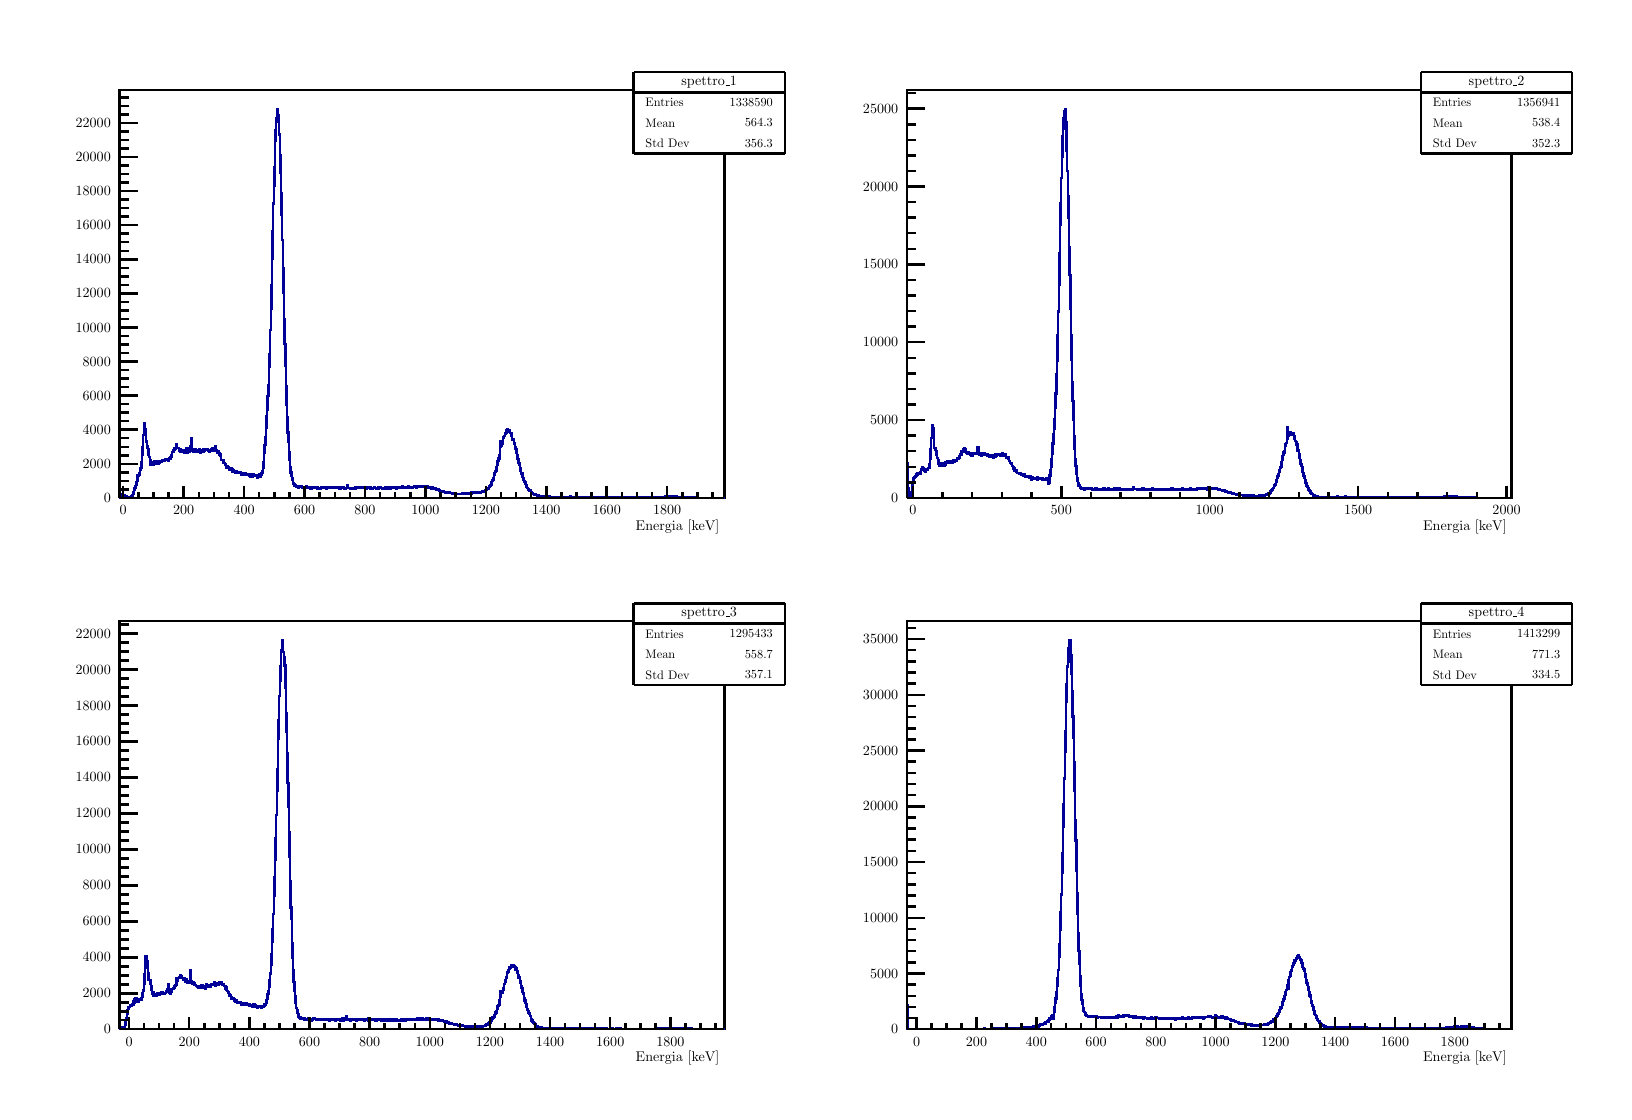
\begin{tikzpicture}
\pgfdeclareplotmark{cross} {
\pgfpathmoveto{\pgfpoint{-0.3\pgfplotmarksize}{\pgfplotmarksize}}
\pgfpathlineto{\pgfpoint{+0.3\pgfplotmarksize}{\pgfplotmarksize}}
\pgfpathlineto{\pgfpoint{+0.3\pgfplotmarksize}{0.3\pgfplotmarksize}}
\pgfpathlineto{\pgfpoint{+1\pgfplotmarksize}{0.3\pgfplotmarksize}}
\pgfpathlineto{\pgfpoint{+1\pgfplotmarksize}{-0.3\pgfplotmarksize}}
\pgfpathlineto{\pgfpoint{+0.3\pgfplotmarksize}{-0.3\pgfplotmarksize}}
\pgfpathlineto{\pgfpoint{+0.3\pgfplotmarksize}{-1.\pgfplotmarksize}}
\pgfpathlineto{\pgfpoint{-0.3\pgfplotmarksize}{-1.\pgfplotmarksize}}
\pgfpathlineto{\pgfpoint{-0.3\pgfplotmarksize}{-0.3\pgfplotmarksize}}
\pgfpathlineto{\pgfpoint{-1.\pgfplotmarksize}{-0.3\pgfplotmarksize}}
\pgfpathlineto{\pgfpoint{-1.\pgfplotmarksize}{0.3\pgfplotmarksize}}
\pgfpathlineto{\pgfpoint{-0.3\pgfplotmarksize}{0.3\pgfplotmarksize}}
\pgfpathclose
\pgfusepathqstroke
}
\pgfdeclareplotmark{cross*} {
\pgfpathmoveto{\pgfpoint{-0.3\pgfplotmarksize}{\pgfplotmarksize}}
\pgfpathlineto{\pgfpoint{+0.3\pgfplotmarksize}{\pgfplotmarksize}}
\pgfpathlineto{\pgfpoint{+0.3\pgfplotmarksize}{0.3\pgfplotmarksize}}
\pgfpathlineto{\pgfpoint{+1\pgfplotmarksize}{0.3\pgfplotmarksize}}
\pgfpathlineto{\pgfpoint{+1\pgfplotmarksize}{-0.3\pgfplotmarksize}}
\pgfpathlineto{\pgfpoint{+0.3\pgfplotmarksize}{-0.3\pgfplotmarksize}}
\pgfpathlineto{\pgfpoint{+0.3\pgfplotmarksize}{-1.\pgfplotmarksize}}
\pgfpathlineto{\pgfpoint{-0.3\pgfplotmarksize}{-1.\pgfplotmarksize}}
\pgfpathlineto{\pgfpoint{-0.3\pgfplotmarksize}{-0.3\pgfplotmarksize}}
\pgfpathlineto{\pgfpoint{-1.\pgfplotmarksize}{-0.3\pgfplotmarksize}}
\pgfpathlineto{\pgfpoint{-1.\pgfplotmarksize}{0.3\pgfplotmarksize}}
\pgfpathlineto{\pgfpoint{-0.3\pgfplotmarksize}{0.3\pgfplotmarksize}}
\pgfpathclose
\pgfusepathqfillstroke
}
\pgfdeclareplotmark{newstar} {
\pgfpathmoveto{\pgfqpoint{0pt}{\pgfplotmarksize}}
\pgfpathlineto{\pgfqpointpolar{44}{0.5\pgfplotmarksize}}
\pgfpathlineto{\pgfqpointpolar{18}{\pgfplotmarksize}}
\pgfpathlineto{\pgfqpointpolar{-20}{0.5\pgfplotmarksize}}
\pgfpathlineto{\pgfqpointpolar{-54}{\pgfplotmarksize}}
\pgfpathlineto{\pgfqpointpolar{-90}{0.5\pgfplotmarksize}}
\pgfpathlineto{\pgfqpointpolar{234}{\pgfplotmarksize}}
\pgfpathlineto{\pgfqpointpolar{198}{0.5\pgfplotmarksize}}
\pgfpathlineto{\pgfqpointpolar{162}{\pgfplotmarksize}}
\pgfpathlineto{\pgfqpointpolar{134}{0.5\pgfplotmarksize}}
\pgfpathclose
\pgfusepathqstroke
}
\pgfdeclareplotmark{newstar*} {
\pgfpathmoveto{\pgfqpoint{0pt}{\pgfplotmarksize}}
\pgfpathlineto{\pgfqpointpolar{44}{0.5\pgfplotmarksize}}
\pgfpathlineto{\pgfqpointpolar{18}{\pgfplotmarksize}}
\pgfpathlineto{\pgfqpointpolar{-20}{0.5\pgfplotmarksize}}
\pgfpathlineto{\pgfqpointpolar{-54}{\pgfplotmarksize}}
\pgfpathlineto{\pgfqpointpolar{-90}{0.5\pgfplotmarksize}}
\pgfpathlineto{\pgfqpointpolar{234}{\pgfplotmarksize}}
\pgfpathlineto{\pgfqpointpolar{198}{0.5\pgfplotmarksize}}
\pgfpathlineto{\pgfqpointpolar{162}{\pgfplotmarksize}}
\pgfpathlineto{\pgfqpointpolar{134}{0.5\pgfplotmarksize}}
\pgfpathclose
\pgfusepathqfillstroke
}
\definecolor{c}{rgb}{1,1,1};
\draw [color=c, fill=c] (0,0) rectangle (20,13.4957);
\draw [color=c, fill=c] (0.2,6.88281) rectangle (9.8,13.3607);
\draw [color=c, fill=c] (1.16,7.5306) rectangle (8.84,12.713);
\definecolor{c}{rgb}{0,0,0};
\draw [c,line width=0.9] (1.16,7.5306) -- (1.16,12.713) -- (8.84,12.713) -- (8.84,7.5306) -- (1.16,7.5306);
\definecolor{c}{rgb}{1,1,1};
\draw [color=c, fill=c] (1.16,7.5306) rectangle (8.84,12.713);
\definecolor{c}{rgb}{0,0,0};
\draw [c,line width=0.9] (1.16,7.5306) -- (1.16,12.713) -- (8.84,12.713) -- (8.84,7.5306) -- (1.16,7.5306);
\definecolor{c}{rgb}{0,0,0.6};
\draw [c,line width=0.9] (1.16,7.80379) -- (1.16768,7.80379) -- (1.16768,7.53125) -- (1.17536,7.53125) -- (1.17536,7.53147) -- (1.18304,7.53147) -- (1.18304,7.54229) -- (1.19072,7.54229) -- (1.19072,7.5661) -- (1.1984,7.5661) -- (1.1984,7.57195) --
 (1.20608,7.57195) -- (1.20608,7.5661) -- (1.21376,7.5661) -- (1.21376,7.56589) -- (1.22144,7.56589) -- (1.22144,7.55744) -- (1.22912,7.55744) -- (1.22912,7.55225) -- (1.2368,7.55225) -- (1.2368,7.54835) -- (1.24448,7.54835) -- (1.24448,7.54575) --
 (1.25216,7.54575) -- (1.25216,7.54337) -- (1.25984,7.54337) -- (1.25984,7.54337) -- (1.26752,7.54337) -- (1.26752,7.54056) -- (1.2752,7.54056) -- (1.2752,7.53991) -- (1.28288,7.53991) -- (1.28288,7.54272) -- (1.29056,7.54272) -- (1.29056,7.54099) --
 (1.29824,7.54099) -- (1.29824,7.54446) -- (1.30592,7.54446) -- (1.30592,7.55008) -- (1.3136,7.55008) -- (1.3136,7.55528) -- (1.32128,7.55528) -- (1.32128,7.56827) -- (1.32896,7.56827) -- (1.32896,7.58061) -- (1.33664,7.58061) -- (1.33664,7.60031) --
 (1.34432,7.60031) -- (1.34432,7.63364) -- (1.352,7.63364) -- (1.352,7.65464) -- (1.35968,7.65464) -- (1.35968,7.68127) -- (1.36736,7.68127) -- (1.36736,7.7001) -- (1.37504,7.7001) -- (1.37504,7.73365) -- (1.38272,7.73365) -- (1.38272,7.75465) --
 (1.3904,7.75465) -- (1.3904,7.81245) -- (1.39808,7.81245) -- (1.39808,7.8092) -- (1.40576,7.8092) -- (1.40576,7.82717) -- (1.41344,7.82717) -- (1.41344,7.84579) -- (1.42112,7.84579) -- (1.42112,7.88324) -- (1.4288,7.88324) -- (1.4288,7.90986) --
 (1.43648,7.90986) -- (1.43648,7.9826) -- (1.44416,7.9826) -- (1.44416,8.0733) -- (1.45184,8.0733) -- (1.45184,8.17872) -- (1.45952,8.17872) -- (1.45952,8.33155) -- (1.4672,8.33155) -- (1.4672,8.41511) -- (1.47488,8.41511) -- (1.47488,8.4846) --
 (1.48256,8.4846) -- (1.48256,8.39736) -- (1.49024,8.39736) -- (1.49024,8.33155) -- (1.49792,8.33155) -- (1.49792,8.24431) -- (1.5056,8.24431) -- (1.5056,8.18305) -- (1.51328,8.18305) -- (1.51328,8.16638) -- (1.52096,8.16638) -- (1.52096,8.14257) --
 (1.52864,8.14257) -- (1.52864,8.08109) -- (1.53632,8.08109) -- (1.53632,8.04905) -- (1.544,8.04905) -- (1.544,8.00792) -- (1.55168,8.00792) -- (1.55168,7.95467) -- (1.55936,7.95467) -- (1.55936,7.95684) -- (1.56704,7.95684) -- (1.56704,7.94666) --
 (1.57472,7.94666) -- (1.57472,7.94969) -- (1.5824,7.94969) -- (1.5824,7.98454) -- (1.59008,7.98454) -- (1.59008,7.95034) -- (1.59776,7.95034) -- (1.59776,7.97134) -- (1.60544,7.97134) -- (1.60544,7.99299) -- (1.61312,7.99299) -- (1.61312,7.96636) --
 (1.6208,7.96636) -- (1.6208,7.9826) -- (1.62848,7.9826) -- (1.62848,7.96073) -- (1.63616,7.96073) -- (1.63616,7.97718) -- (1.64384,7.97718) -- (1.64384,8.00056) -- (1.65152,8.00056) -- (1.65152,7.9642) -- (1.6592,7.9642) -- (1.6592,7.9787) --
 (1.66688,7.9787) -- (1.66688,7.99212) -- (1.67456,7.99212) -- (1.67456,7.99277) -- (1.68224,7.99277) -- (1.68224,7.99753) -- (1.68992,7.99753) -- (1.68992,7.99277) -- (1.6976,7.99277) -- (1.6976,8.0023) -- (1.70528,8.0023) -- (1.70528,8.01312) --
 (1.71296,8.01312) -- (1.71296,8.00338) -- (1.72064,8.00338) -- (1.72064,7.99688) -- (1.72832,7.99688) -- (1.72832,8.01182) -- (1.736,8.01182) -- (1.736,8.0155) -- (1.74368,8.0155) -- (1.74368,8.02373) -- (1.75136,8.02373) -- (1.75136,8.01442) --
 (1.75904,8.01442) -- (1.75904,8.01355) -- (1.76672,8.01355) -- (1.76672,8.0116) -- (1.7744,8.0116) -- (1.7744,8.02719) -- (1.78208,8.02719) -- (1.78208,8.00641) -- (1.78976,8.00641) -- (1.78976,8.03931) -- (1.79744,8.03931) -- (1.79744,8.03087) --
 (1.80512,8.03087) -- (1.80512,8.05143) -- (1.8128,8.05143) -- (1.8128,8.05879) -- (1.82048,8.05879) -- (1.82048,8.0733) -- (1.82816,8.0733) -- (1.82816,8.11421) -- (1.83584,8.11421) -- (1.83584,8.11508) -- (1.84352,8.11508) -- (1.84352,8.14105) --
 (1.8512,8.14105) -- (1.8512,8.16313) -- (1.85888,8.16313) -- (1.85888,8.14538) -- (1.86656,8.14538) -- (1.86656,8.15816) -- (1.87424,8.15816) -- (1.87424,8.19106) -- (1.88192,8.19106) -- (1.88192,8.21336) -- (1.8896,8.21336) -- (1.8896,8.1653) --
 (1.89728,8.1653) -- (1.89728,8.16746) -- (1.90496,8.16746) -- (1.90496,8.16184) -- (1.91264,8.16184) -- (1.91264,8.12504) -- (1.92032,8.12504) -- (1.92032,8.15015) -- (1.928,8.15015) -- (1.928,8.14668) -- (1.93568,8.14668) -- (1.93568,8.12222) --
 (1.94336,8.12222) -- (1.94336,8.13175) -- (1.95104,8.13175) -- (1.95104,8.13196) -- (1.95872,8.13196) -- (1.95872,8.12417) -- (1.9664,8.12417) -- (1.9664,8.12157) -- (1.97408,8.12157) -- (1.97408,8.12612) -- (1.98176,8.12612) -- (1.98176,8.10685) --
 (1.98944,8.10685) -- (1.98944,8.1298) -- (1.99712,8.1298) -- (1.99712,8.11335) -- (2.0048,8.11335) -- (2.0048,8.13759) -- (2.01248,8.13759) -- (2.01248,8.15621) -- (2.02016,8.15621) -- (2.02016,8.09992) -- (2.02784,8.09992) -- (2.02784,8.13456) --
 (2.03552,8.13456) -- (2.03552,8.12612) -- (2.0432,8.12612) -- (2.0432,8.11464) -- (2.05088,8.11464) -- (2.05088,8.14019) -- (2.05856,8.14019) -- (2.05856,8.1811) -- (2.06624,8.1811) -- (2.06624,8.29345) -- (2.07392,8.29345) -- (2.07392,8.1614) --
 (2.0816,8.1614) -- (2.0816,8.1482) -- (2.08928,8.1482) -- (2.08928,8.13543) -- (2.09696,8.13543) -- (2.09696,8.11313) -- (2.10464,8.11313) -- (2.10464,8.13499) -- (2.11232,8.13499) -- (2.11232,8.14127) -- (2.12,8.14127) -- (2.12,8.15015) --
 (2.12768,8.15015) -- (2.12768,8.13932) -- (2.13536,8.13932) -- (2.13536,8.11421) -- (2.14304,8.11421) -- (2.14304,8.11897) -- (2.15072,8.11897) -- (2.15072,8.13781) -- (2.1584,8.13781) -- (2.1584,8.1417) -- (2.16608,8.1417) -- (2.16608,8.14452) --
 (2.17376,8.14452) -- (2.17376,8.13543) -- (2.18144,8.13543) -- (2.18144,8.10707) -- (2.18912,8.10707) -- (2.18912,8.12677) -- (2.1968,8.12677) -- (2.1968,8.12244) -- (2.20448,8.12244) -- (2.20448,8.11616) -- (2.21216,8.11616) -- (2.21216,8.13543) --
 (2.21984,8.13543) -- (2.21984,8.1443) -- (2.22752,8.1443) -- (2.22752,8.11486) -- (2.2352,8.11486) -- (2.2352,8.12374) -- (2.24288,8.12374) -- (2.24288,8.14387) -- (2.25056,8.14387) -- (2.25056,8.13651) -- (2.25824,8.13651) -- (2.25824,8.14019) --
 (2.26592,8.14019) -- (2.26592,8.14538) -- (2.2736,8.14538) -- (2.2736,8.14495) -- (2.28128,8.14495) -- (2.28128,8.1272) -- (2.28896,8.1272) -- (2.28896,8.13326) -- (2.29664,8.13326) -- (2.29664,8.11962) -- (2.30432,8.11962) -- (2.30432,8.13802) --
 (2.312,8.13802) -- (2.312,8.13239) -- (2.31968,8.13239) -- (2.31968,8.14603) -- (2.32736,8.14603) -- (2.32736,8.13694) -- (2.33504,8.13694) -- (2.33504,8.15794) -- (2.34272,8.15794) -- (2.34272,8.13456) -- (2.3504,8.13456) -- (2.3504,8.14538) --
 (2.35808,8.14538) -- (2.35808,8.14625) -- (2.36576,8.14625) -- (2.36576,8.14993) -- (2.37344,8.14993) -- (2.37344,8.1811) -- (2.38112,8.1811) -- (2.38112,8.1298) -- (2.3888,8.1298) -- (2.3888,8.1246) -- (2.39648,8.1246) -- (2.39648,8.10469) --
 (2.40416,8.10469) -- (2.40416,8.12698) -- (2.41184,8.12698) -- (2.41184,8.12395) -- (2.41952,8.12395) -- (2.41952,8.10404) -- (2.4272,8.10404) -- (2.4272,8.08087) -- (2.43488,8.08087) -- (2.43488,8.0891) -- (2.44256,8.0891) -- (2.44256,8.06053) --
 (2.45024,8.06053) -- (2.45024,8.0129) -- (2.45792,8.0129) -- (2.45792,8.00944) -- (2.4656,8.00944) -- (2.4656,8.01398) -- (2.47328,8.01398) -- (2.47328,8.0116) -- (2.48096,8.0116) -- (2.48096,7.97307) -- (2.48864,7.97307) -- (2.48864,7.97589) --
 (2.49632,7.97589) -- (2.49632,7.96225) -- (2.504,7.96225) -- (2.504,7.94839) -- (2.51168,7.94839) -- (2.51168,7.92826) -- (2.51936,7.92826) -- (2.51936,7.91917) -- (2.52704,7.91917) -- (2.52704,7.93021) -- (2.53472,7.93021) -- (2.53472,7.9235) --
 (2.5424,7.9235) -- (2.5424,7.91679) -- (2.55008,7.91679) -- (2.55008,7.9025) -- (2.55776,7.9025) -- (2.55776,7.89428) -- (2.56544,7.89428) -- (2.56544,7.89341) -- (2.57312,7.89341) -- (2.57312,7.90337) -- (2.5808,7.90337) -- (2.5808,7.88194) --
 (2.58848,7.88194) -- (2.58848,7.89536) -- (2.59616,7.89536) -- (2.59616,7.85877) -- (2.60384,7.85877) -- (2.60384,7.88388) -- (2.61152,7.88388) -- (2.61152,7.87436) -- (2.6192,7.87436) -- (2.6192,7.86029) -- (2.62688,7.86029) -- (2.62688,7.86462) --
 (2.63456,7.86462) -- (2.63456,7.84557) -- (2.64224,7.84557) -- (2.64224,7.86548) -- (2.64992,7.86548) -- (2.64992,7.85812) -- (2.6576,7.85812) -- (2.6576,7.85618) -- (2.66528,7.85618) -- (2.66528,7.84687) -- (2.67296,7.84687) -- (2.67296,7.85704) --
 (2.68064,7.85704) -- (2.68064,7.84947) -- (2.68832,7.84947) -- (2.68832,7.85769) -- (2.696,7.85769) -- (2.696,7.85401) -- (2.70368,7.85401) -- (2.70368,7.83886) -- (2.71136,7.83886) -- (2.71136,7.82803) -- (2.71904,7.82803) -- (2.71904,7.83972) --
 (2.72672,7.83972) -- (2.72672,7.83518) -- (2.7344,7.83518) -- (2.7344,7.84124) -- (2.74208,7.84124) -- (2.74208,7.83085) -- (2.74976,7.83085) -- (2.74976,7.83756) -- (2.75744,7.83756) -- (2.75744,7.84037) -- (2.76512,7.84037) -- (2.76512,7.83475) --
 (2.7728,7.83475) -- (2.7728,7.8289) -- (2.78048,7.8289) -- (2.78048,7.8276) -- (2.78816,7.8276) -- (2.78816,7.82609) -- (2.79584,7.82609) -- (2.79584,7.8289) -- (2.80352,7.8289) -- (2.80352,7.81764) -- (2.8112,7.81764) -- (2.8112,7.81743) --
 (2.81888,7.81743) -- (2.81888,7.80487) -- (2.82656,7.80487) -- (2.82656,7.81764) -- (2.83424,7.81764) -- (2.83424,7.8302) -- (2.84192,7.8302) -- (2.84192,7.80098) -- (2.8496,7.80098) -- (2.8496,7.81266) -- (2.85728,7.81266) -- (2.85728,7.82868) --
 (2.86496,7.82868) -- (2.86496,7.82089) -- (2.87264,7.82089) -- (2.87264,7.80855) -- (2.88032,7.80855) -- (2.88032,7.80963) -- (2.888,7.80963) -- (2.888,7.82132) -- (2.89568,7.82132) -- (2.89568,7.82306) -- (2.90336,7.82306) -- (2.90336,7.78994) --
 (2.91104,7.78994) -- (2.91104,7.80292) -- (2.91872,7.80292) -- (2.91872,7.80834) -- (2.9264,7.80834) -- (2.9264,7.80704) -- (2.93408,7.80704) -- (2.93408,7.82998) -- (2.94176,7.82998) -- (2.94176,7.80271) -- (2.94944,7.80271) -- (2.94944,7.82067) --
 (2.95712,7.82067) -- (2.95712,7.82825) -- (2.9648,7.82825) -- (2.9648,7.8473) -- (2.97248,7.8473) -- (2.97248,7.87371) -- (2.98016,7.87371) -- (2.98016,7.91462) -- (2.98784,7.91462) -- (2.98784,7.98433) -- (2.99552,7.98433) -- (2.99552,8.10079) --
 (3.0032,8.10079) -- (3.0032,8.2008) -- (3.01088,8.2008) -- (3.01088,8.30362) -- (3.01856,8.30362) -- (3.01856,8.42615) -- (3.02624,8.42615) -- (3.02624,8.56469) -- (3.03392,8.56469) -- (3.03392,8.65409) -- (3.0416,8.65409) -- (3.0416,8.82381) --
 (3.04928,8.82381) -- (3.04928,8.96192) -- (3.05696,8.96192) -- (3.05696,9.2022) -- (3.06464,9.2022) -- (3.06464,9.35178) -- (3.07232,9.35178) -- (3.07232,9.66459) -- (3.08,9.66459) -- (3.08,9.93756) -- (3.08768,9.93756) -- (3.08768,10.2313) --
 (3.09536,10.2313) -- (3.09536,10.5675) -- (3.10304,10.5675) -- (3.10304,10.9195) -- (3.11072,10.9195) -- (3.11072,11.2693) -- (3.1184,11.2693) -- (3.1184,11.4912) -- (3.12608,11.4912) -- (3.12608,11.7341) -- (3.13376,11.7341) -- (3.13376,12.072) --
 (3.14144,12.072) -- (3.14144,12.2003) -- (3.14912,12.2003) -- (3.14912,12.3545) -- (3.1568,12.3545) -- (3.1568,12.3952) -- (3.16448,12.3952) -- (3.16448,12.4662) -- (3.17216,12.4662) -- (3.17216,12.309) -- (3.17984,12.309) -- (3.17984,12.3874) --
 (3.18752,12.3874) -- (3.18752,12.1475) -- (3.1952,12.1475) -- (3.1952,11.8761) -- (3.20288,11.8761) -- (3.20288,11.6585) -- (3.21056,11.6585) -- (3.21056,11.4052) -- (3.21824,11.4052) -- (3.21824,11.1217) -- (3.22592,11.1217) -- (3.22592,10.8076) --
 (3.2336,10.8076) -- (3.2336,10.445) -- (3.24128,10.445) -- (3.24128,10.1397) -- (3.24896,10.1397) -- (3.24896,9.7949) -- (3.25664,9.7949) -- (3.25664,9.48232) -- (3.26432,9.48232) -- (3.26432,9.20631) -- (3.272,9.20631) -- (3.272,8.95066) --
 (3.27968,8.95066) -- (3.27968,8.71839) -- (3.28736,8.71839) -- (3.28736,8.55084) -- (3.29504,8.55084) -- (3.29504,8.36229) -- (3.30272,8.36229) -- (3.30272,8.23868) -- (3.3104,8.23868) -- (3.3104,8.1062) -- (3.31808,8.1062) -- (3.31808,8.01312) --
 (3.32576,8.01312) -- (3.32576,7.9261) -- (3.33344,7.9261) -- (3.33344,7.85509) -- (3.34112,7.85509) -- (3.34112,7.81829) -- (3.3488,7.81829) -- (3.3488,7.77413) -- (3.35648,7.77413) -- (3.35648,7.7553) -- (3.36416,7.7553) -- (3.36416,7.72153) --
 (3.37184,7.72153) -- (3.37184,7.70984) -- (3.37952,7.70984) -- (3.37952,7.68473) -- (3.3872,7.68473) -- (3.3872,7.69057) -- (3.39488,7.69057) -- (3.39488,7.68473) -- (3.40256,7.68473) -- (3.40256,7.67304) -- (3.41024,7.67304) -- (3.41024,7.68408) --
 (3.41792,7.68408) -- (3.41792,7.67261) -- (3.4256,7.67261) -- (3.4256,7.67607) -- (3.43328,7.67607) -- (3.43328,7.66525) -- (3.44096,7.66525) -- (3.44096,7.67282) -- (3.44864,7.67282) -- (3.44864,7.66871) -- (3.45632,7.66871) -- (3.45632,7.66828) --
 (3.464,7.66828) -- (3.464,7.67282) -- (3.47168,7.67282) -- (3.47168,7.66849) -- (3.47936,7.66849) -- (3.47936,7.65681) -- (3.48704,7.65681) -- (3.48704,7.67109) -- (3.49472,7.67109) -- (3.49472,7.66135) -- (3.5024,7.66135) -- (3.5024,7.6659) --
 (3.51008,7.6659) -- (3.51008,7.66546) -- (3.51776,7.66546) -- (3.51776,7.66352) -- (3.52544,7.66352) -- (3.52544,7.67607) -- (3.53312,7.67607) -- (3.53312,7.66135) -- (3.5408,7.66135) -- (3.5408,7.65745) -- (3.54848,7.65745) -- (3.54848,7.66178) --
 (3.55616,7.66178) -- (3.55616,7.66308) -- (3.56384,7.66308) -- (3.56384,7.66546) -- (3.57152,7.66546) -- (3.57152,7.65659) -- (3.5792,7.65659) -- (3.5792,7.66135) -- (3.58688,7.66135) -- (3.58688,7.65204) -- (3.59456,7.65204) -- (3.59456,7.6607) --
 (3.60224,7.6607) -- (3.60224,7.65767) -- (3.60992,7.65767) -- (3.60992,7.65984) -- (3.6176,7.65984) -- (3.6176,7.65745) -- (3.62528,7.65745) -- (3.62528,7.66373) -- (3.63296,7.66373) -- (3.63296,7.66611) -- (3.64064,7.66611) -- (3.64064,7.65399) --
 (3.64832,7.65399) -- (3.64832,7.66222) -- (3.656,7.66222) -- (3.656,7.65962) -- (3.66368,7.65962) -- (3.66368,7.66049) -- (3.67136,7.66049) -- (3.67136,7.65226) -- (3.67904,7.65226) -- (3.67904,7.65875) -- (3.68672,7.65875) -- (3.68672,7.65139) --
 (3.6944,7.65139) -- (3.6944,7.65854) -- (3.70208,7.65854) -- (3.70208,7.64338) -- (3.70976,7.64338) -- (3.70976,7.65269) -- (3.71744,7.65269) -- (3.71744,7.66092) -- (3.72512,7.66092) -- (3.72512,7.662) -- (3.7328,7.662) -- (3.7328,7.65356) --
 (3.74048,7.65356) -- (3.74048,7.65919) -- (3.74816,7.65919) -- (3.74816,7.67131) -- (3.75584,7.67131) -- (3.75584,7.65616) -- (3.76352,7.65616) -- (3.76352,7.66395) -- (3.7712,7.66395) -- (3.7712,7.66785) -- (3.77888,7.66785) -- (3.77888,7.65356) --
 (3.78656,7.65356) -- (3.78656,7.6475) -- (3.79424,7.6475) -- (3.79424,7.66655) -- (3.80192,7.66655) -- (3.80192,7.66373) -- (3.8096,7.66373) -- (3.8096,7.65724) -- (3.81728,7.65724) -- (3.81728,7.6646) -- (3.82496,7.6646) -- (3.82496,7.65551) --
 (3.83264,7.65551) -- (3.83264,7.65377) -- (3.84032,7.65377) -- (3.84032,7.66395) -- (3.848,7.66395) -- (3.848,7.6607) -- (3.85568,7.6607) -- (3.85568,7.65616) -- (3.86336,7.65616) -- (3.86336,7.6646) -- (3.87104,7.6646) -- (3.87104,7.66113) --
 (3.87872,7.66113) -- (3.87872,7.66525) -- (3.8864,7.66525) -- (3.8864,7.65356) -- (3.89408,7.65356) -- (3.89408,7.66005) -- (3.90176,7.66005) -- (3.90176,7.65356) -- (3.90944,7.65356) -- (3.90944,7.65789) -- (3.91712,7.65789) -- (3.91712,7.65745) --
 (3.9248,7.65745) -- (3.9248,7.65421) -- (3.93248,7.65421) -- (3.93248,7.66503) -- (3.94016,7.66503) -- (3.94016,7.65789) -- (3.94784,7.65789) -- (3.94784,7.64728) -- (3.95552,7.64728) -- (3.95552,7.65118) -- (3.9632,7.65118) -- (3.9632,7.65897) --
 (3.97088,7.65897) -- (3.97088,7.65745) -- (3.97856,7.65745) -- (3.97856,7.66005) -- (3.98624,7.66005) -- (3.98624,7.65681) -- (3.99392,7.65681) -- (3.99392,7.66135) -- (4.0016,7.66135) -- (4.0016,7.65529) -- (4.00928,7.65529) -- (4.00928,7.65248) --
 (4.01696,7.65248) -- (4.01696,7.65421) -- (4.02464,7.65421) -- (4.02464,7.6449) -- (4.03232,7.6449) -- (4.03232,7.65854) -- (4.04,7.65854) -- (4.04,7.65702) -- (4.04768,7.65702) -- (4.04768,7.66893) -- (4.05536,7.66893) -- (4.05536,7.69187) --
 (4.06304,7.69187) -- (4.06304,7.65659) -- (4.07072,7.65659) -- (4.07072,7.65637) -- (4.0784,7.65637) -- (4.0784,7.65789) -- (4.08608,7.65789) -- (4.08608,7.65313) -- (4.09376,7.65313) -- (4.09376,7.65789) -- (4.10144,7.65789) -- (4.10144,7.65356) --
 (4.10912,7.65356) -- (4.10912,7.65767) -- (4.1168,7.65767) -- (4.1168,7.65291) -- (4.12448,7.65291) -- (4.12448,7.65269) -- (4.13216,7.65269) -- (4.13216,7.64576) -- (4.13984,7.64576) -- (4.13984,7.65767) -- (4.14752,7.65767) -- (4.14752,7.66503) --
 (4.1552,7.66503) -- (4.1552,7.65269) -- (4.16288,7.65269) -- (4.16288,7.65854) -- (4.17056,7.65854) -- (4.17056,7.66265) -- (4.17824,7.66265) -- (4.17824,7.66157) -- (4.18592,7.66157) -- (4.18592,7.66308) -- (4.1936,7.66308) -- (4.1936,7.65681) --
 (4.20128,7.65681) -- (4.20128,7.65962) -- (4.20896,7.65962) -- (4.20896,7.66698) -- (4.21664,7.66698) -- (4.21664,7.66849) -- (4.22432,7.66849) -- (4.22432,7.65572) -- (4.232,7.65572) -- (4.232,7.65637) -- (4.23968,7.65637) -- (4.23968,7.65486) --
 (4.24736,7.65486) -- (4.24736,7.65702) -- (4.25504,7.65702) -- (4.25504,7.66243) -- (4.26272,7.66243) -- (4.26272,7.66849) -- (4.2704,7.66849) -- (4.2704,7.65356) -- (4.27808,7.65356) -- (4.27808,7.64901) -- (4.28576,7.64901) -- (4.28576,7.6607) --
 (4.29344,7.6607) -- (4.29344,7.65139) -- (4.30112,7.65139) -- (4.30112,7.662) -- (4.3088,7.662) -- (4.3088,7.65442) -- (4.31648,7.65442) -- (4.31648,7.65789) -- (4.32416,7.65789) -- (4.32416,7.65377) -- (4.33184,7.65377) -- (4.33184,7.66893) --
 (4.33952,7.66893) -- (4.33952,7.66655) -- (4.3472,7.66655) -- (4.3472,7.65139) -- (4.35488,7.65139) -- (4.35488,7.65204) -- (4.36256,7.65204) -- (4.36256,7.65551) -- (4.37024,7.65551) -- (4.37024,7.64815) -- (4.37792,7.64815) -- (4.37792,7.65616) --
 (4.3856,7.65616) -- (4.3856,7.65659) -- (4.39328,7.65659) -- (4.39328,7.66525) -- (4.40096,7.66525) -- (4.40096,7.65356) -- (4.40864,7.65356) -- (4.40864,7.65767) -- (4.41632,7.65767) -- (4.41632,7.6462) -- (4.424,7.6462) -- (4.424,7.65442) --
 (4.43168,7.65442) -- (4.43168,7.65897) -- (4.43936,7.65897) -- (4.43936,7.64836) -- (4.44704,7.64836) -- (4.44704,7.66438) -- (4.45472,7.66438) -- (4.45472,7.66395) -- (4.4624,7.66395) -- (4.4624,7.66914) -- (4.47008,7.66914) -- (4.47008,7.65984) --
 (4.47776,7.65984) -- (4.47776,7.65572) -- (4.48544,7.65572) -- (4.48544,7.65875) -- (4.49312,7.65875) -- (4.49312,7.64728) -- (4.5008,7.64728) -- (4.5008,7.6462) -- (4.50848,7.6462) -- (4.50848,7.65074) -- (4.51616,7.65074) -- (4.51616,7.65529) --
 (4.52384,7.65529) -- (4.52384,7.65919) -- (4.53152,7.65919) -- (4.53152,7.662) -- (4.5392,7.662) -- (4.5392,7.6462) -- (4.54688,7.6462) -- (4.54688,7.64923) -- (4.55456,7.64923) -- (4.55456,7.66785) -- (4.56224,7.66785) -- (4.56224,7.65118) --
 (4.56992,7.65118) -- (4.56992,7.662) -- (4.5776,7.662) -- (4.5776,7.66113) -- (4.58528,7.66113) -- (4.58528,7.6594) -- (4.59296,7.6594) -- (4.59296,7.65313) -- (4.60064,7.65313) -- (4.60064,7.65702) -- (4.60832,7.65702) -- (4.60832,7.66135) --
 (4.616,7.66135) -- (4.616,7.6633) -- (4.62368,7.6633) -- (4.62368,7.6607) -- (4.63136,7.6607) -- (4.63136,7.66092) -- (4.63904,7.66092) -- (4.63904,7.66438) -- (4.64672,7.66438) -- (4.64672,7.65789) -- (4.6544,7.65789) -- (4.6544,7.66222) --
 (4.66208,7.66222) -- (4.66208,7.66417) -- (4.66976,7.66417) -- (4.66976,7.64966) -- (4.67744,7.64966) -- (4.67744,7.65724) -- (4.68512,7.65724) -- (4.68512,7.65745) -- (4.6928,7.65745) -- (4.6928,7.66005) -- (4.70048,7.66005) -- (4.70048,7.65659) --
 (4.70816,7.65659) -- (4.70816,7.66092) -- (4.71584,7.66092) -- (4.71584,7.66222) -- (4.72352,7.66222) -- (4.72352,7.65919) -- (4.7312,7.65919) -- (4.7312,7.65724) -- (4.73888,7.65724) -- (4.73888,7.66049) -- (4.74656,7.66049) -- (4.74656,7.6633) --
 (4.75424,7.6633) -- (4.75424,7.67304) -- (4.76192,7.67304) -- (4.76192,7.66287) -- (4.7696,7.66287) -- (4.7696,7.66611) -- (4.77728,7.66611) -- (4.77728,7.662) -- (4.78496,7.662) -- (4.78496,7.66525) -- (4.79264,7.66525) -- (4.79264,7.65572) --
 (4.80032,7.65572) -- (4.80032,7.662) -- (4.808,7.662) -- (4.808,7.6659) -- (4.81568,7.6659) -- (4.81568,7.6594) -- (4.82336,7.6594) -- (4.82336,7.67521) -- (4.83104,7.67521) -- (4.83104,7.67629) -- (4.83872,7.67629) -- (4.83872,7.66893) --
 (4.8464,7.66893) -- (4.8464,7.67196) -- (4.85408,7.67196) -- (4.85408,7.65875) -- (4.86176,7.65875) -- (4.86176,7.6659) -- (4.86944,7.6659) -- (4.86944,7.66178) -- (4.87712,7.66178) -- (4.87712,7.66417) -- (4.8848,7.66417) -- (4.8848,7.66849) --
 (4.89248,7.66849) -- (4.89248,7.67088) -- (4.90016,7.67088) -- (4.90016,7.66828) -- (4.90784,7.66828) -- (4.90784,7.6791) -- (4.91552,7.6791) -- (4.91552,7.67217) -- (4.9232,7.67217) -- (4.9232,7.6646) -- (4.93088,7.6646) -- (4.93088,7.66958) --
 (4.93856,7.66958) -- (4.93856,7.67932) -- (4.94624,7.67932) -- (4.94624,7.67456) -- (4.95392,7.67456) -- (4.95392,7.67066) -- (4.9616,7.67066) -- (4.9616,7.67044) -- (4.96928,7.67044) -- (4.96928,7.66655) -- (4.97696,7.66655) -- (4.97696,7.67044) --
 (4.98464,7.67044) -- (4.98464,7.67845) -- (4.99232,7.67845) -- (4.99232,7.67109) -- (5,7.67109) -- (5,7.67391) -- (5.00768,7.67391) -- (5.00768,7.67261) -- (5.01536,7.67261) -- (5.01536,7.66828) -- (5.02304,7.66828) -- (5.02304,7.66633) --
 (5.03072,7.66633) -- (5.03072,7.67304) -- (5.0384,7.67304) -- (5.0384,7.67088) -- (5.04608,7.67088) -- (5.04608,7.67023) -- (5.05376,7.67023) -- (5.05376,7.66417) -- (5.06144,7.66417) -- (5.06144,7.67326) -- (5.06912,7.67326) -- (5.06912,7.6659) --
 (5.0768,7.6659) -- (5.0768,7.6672) -- (5.08448,7.6672) -- (5.08448,7.66005) -- (5.09216,7.66005) -- (5.09216,7.66005) -- (5.09984,7.66005) -- (5.09984,7.65984) -- (5.10752,7.65984) -- (5.10752,7.6633) -- (5.1152,7.6633) -- (5.1152,7.66352) --
 (5.12288,7.66352) -- (5.12288,7.64988) -- (5.13056,7.64988) -- (5.13056,7.66157) -- (5.13824,7.66157) -- (5.13824,7.65356) -- (5.14592,7.65356) -- (5.14592,7.65594) -- (5.1536,7.65594) -- (5.1536,7.65074) -- (5.16128,7.65074) -- (5.16128,7.65139) --
 (5.16896,7.65139) -- (5.16896,7.6475) -- (5.17664,7.6475) -- (5.17664,7.64338) -- (5.18432,7.64338) -- (5.18432,7.63732) -- (5.192,7.63732) -- (5.192,7.64641) -- (5.19968,7.64641) -- (5.19968,7.63949) -- (5.20736,7.63949) -- (5.20736,7.64273) --
 (5.21504,7.64273) -- (5.21504,7.63213) -- (5.22272,7.63213) -- (5.22272,7.62715) -- (5.2304,7.62715) -- (5.2304,7.62022) -- (5.23808,7.62022) -- (5.23808,7.62) -- (5.24576,7.62) -- (5.24576,7.62022) -- (5.25344,7.62022) -- (5.25344,7.61892) --
 (5.26112,7.61892) -- (5.26112,7.61849) -- (5.2688,7.61849) -- (5.2688,7.61459) -- (5.27648,7.61459) -- (5.27648,7.60399) -- (5.28416,7.60399) -- (5.28416,7.60334) -- (5.29184,7.60334) -- (5.29184,7.60723) -- (5.29952,7.60723) -- (5.29952,7.60225) --
 (5.3072,7.60225) -- (5.3072,7.59922) -- (5.31488,7.59922) -- (5.31488,7.60334) -- (5.32256,7.60334) -- (5.32256,7.60377) -- (5.33024,7.60377) -- (5.33024,7.59814) -- (5.33792,7.59814) -- (5.33792,7.59641) -- (5.3456,7.59641) -- (5.3456,7.59749) --
 (5.35328,7.59749) -- (5.35328,7.591) -- (5.36096,7.591) -- (5.36096,7.59121) -- (5.36864,7.59121) -- (5.36864,7.59251) -- (5.37632,7.59251) -- (5.37632,7.59035) -- (5.384,7.59035) -- (5.384,7.5884) -- (5.39168,7.5884) -- (5.39168,7.59121) --
 (5.39936,7.59121) -- (5.39936,7.58775) -- (5.40704,7.58775) -- (5.40704,7.5858) -- (5.41472,7.5858) -- (5.41472,7.591) -- (5.4224,7.591) -- (5.4224,7.5884) -- (5.43008,7.5884) -- (5.43008,7.58126) -- (5.43776,7.58126) -- (5.43776,7.58082) --
 (5.44544,7.58082) -- (5.44544,7.58017) -- (5.45312,7.58017) -- (5.45312,7.57714) -- (5.4608,7.57714) -- (5.4608,7.58169) -- (5.46848,7.58169) -- (5.46848,7.58277) -- (5.47616,7.58277) -- (5.47616,7.57952) -- (5.48384,7.57952) -- (5.48384,7.57801) --
 (5.49152,7.57801) -- (5.49152,7.57736) -- (5.4992,7.57736) -- (5.4992,7.58299) -- (5.50688,7.58299) -- (5.50688,7.57952) -- (5.51456,7.57952) -- (5.51456,7.58429) -- (5.52224,7.58429) -- (5.52224,7.57801) -- (5.52992,7.57801) -- (5.52992,7.58342) --
 (5.5376,7.58342) -- (5.5376,7.58753) -- (5.54528,7.58753) -- (5.54528,7.58191) -- (5.55296,7.58191) -- (5.55296,7.58342) -- (5.56064,7.58342) -- (5.56064,7.58948) -- (5.56832,7.58948) -- (5.56832,7.58732) -- (5.576,7.58732) -- (5.576,7.58494) --
 (5.58368,7.58494) -- (5.58368,7.58472) -- (5.59136,7.58472) -- (5.59136,7.58797) -- (5.59904,7.58797) -- (5.59904,7.58992) -- (5.60672,7.58992) -- (5.60672,7.58429) -- (5.6144,7.58429) -- (5.6144,7.5936) -- (5.62208,7.5936) -- (5.62208,7.59944) --
 (5.62976,7.59944) -- (5.62976,7.58753) -- (5.63744,7.58753) -- (5.63744,7.60009) -- (5.64512,7.60009) -- (5.64512,7.59013) -- (5.6528,7.59013) -- (5.6528,7.59641) -- (5.66048,7.59641) -- (5.66048,7.59273) -- (5.66816,7.59273) -- (5.66816,7.59576) --
 (5.67584,7.59576) -- (5.67584,7.60464) -- (5.68352,7.60464) -- (5.68352,7.59598) -- (5.6912,7.59598) -- (5.6912,7.59728) -- (5.69888,7.59728) -- (5.69888,7.59879) -- (5.70656,7.59879) -- (5.70656,7.59706) -- (5.71424,7.59706) -- (5.71424,7.59987) --
 (5.72192,7.59987) -- (5.72192,7.6016) -- (5.7296,7.6016) -- (5.7296,7.60096) -- (5.73728,7.60096) -- (5.73728,7.60031) -- (5.74496,7.60031) -- (5.74496,7.60269) -- (5.75264,7.60269) -- (5.75264,7.60334) -- (5.76032,7.60334) -- (5.76032,7.61264) --
 (5.768,7.61264) -- (5.768,7.60442) -- (5.77568,7.60442) -- (5.77568,7.6107) -- (5.78336,7.6107) -- (5.78336,7.61459) -- (5.79104,7.61459) -- (5.79104,7.60896) -- (5.79872,7.60896) -- (5.79872,7.61892) -- (5.8064,7.61892) -- (5.8064,7.63364) --
 (5.81408,7.63364) -- (5.81408,7.63083) -- (5.82176,7.63083) -- (5.82176,7.63537) -- (5.82944,7.63537) -- (5.82944,7.6462) -- (5.83712,7.6462) -- (5.83712,7.64771) -- (5.8448,7.64771) -- (5.8448,7.65399) -- (5.85248,7.65399) -- (5.85248,7.67066) --
 (5.86016,7.67066) -- (5.86016,7.68408) -- (5.86784,7.68408) -- (5.86784,7.69555) -- (5.87552,7.69555) -- (5.87552,7.70226) -- (5.8832,7.70226) -- (5.8832,7.72889) -- (5.89088,7.72889) -- (5.89088,7.74448) -- (5.89856,7.74448) -- (5.89856,7.75898) --
 (5.90624,7.75898) -- (5.90624,7.78582) -- (5.91392,7.78582) -- (5.91392,7.82089) -- (5.9216,7.82089) -- (5.9216,7.83799) -- (5.92928,7.83799) -- (5.92928,7.86354) -- (5.93696,7.86354) -- (5.93696,7.87371) -- (5.94464,7.87371) -- (5.94464,7.91679) --
 (5.95232,7.91679) -- (5.95232,7.95164) -- (5.96,7.95164) -- (5.96,7.99234) -- (5.96768,7.99234) -- (5.96768,8.00424) -- (5.97536,8.00424) -- (5.97536,8.0287) -- (5.98304,8.0287) -- (5.98304,8.06854) -- (5.99072,8.06854) -- (5.99072,8.17959) --
 (5.9984,8.17959) -- (5.9984,8.25427) -- (6.00608,8.25427) -- (6.00608,8.1969) -- (6.01376,8.1969) -- (6.01376,8.22007) -- (6.02144,8.22007) -- (6.02144,8.22894) -- (6.02912,8.22894) -- (6.02912,8.29367) -- (6.0368,8.29367) -- (6.0368,8.30427) --
 (6.04448,8.30427) -- (6.04448,8.31964) -- (6.05216,8.31964) -- (6.05216,8.34973) -- (6.05984,8.34973) -- (6.05984,8.35147) -- (6.06752,8.35147) -- (6.06752,8.35276) -- (6.0752,8.35276) -- (6.0752,8.39281) -- (6.08288,8.39281) -- (6.08288,8.39844) --
 (6.09056,8.39844) -- (6.09056,8.36965) -- (6.09824,8.36965) -- (6.09824,8.39541) -- (6.10592,8.39541) -- (6.10592,8.38588) -- (6.1136,8.38588) -- (6.1136,8.38545) -- (6.12128,8.38545) -- (6.12128,8.35601) -- (6.12896,8.35601) -- (6.12896,8.348) --
 (6.13664,8.348) -- (6.13664,8.32289) -- (6.14432,8.32289) -- (6.14432,8.27267) -- (6.152,8.27267) -- (6.152,8.26661) -- (6.15968,8.26661) -- (6.15968,8.27159) -- (6.16736,8.27159) -- (6.16736,8.22526) -- (6.17504,8.22526) -- (6.17504,8.21487) --
 (6.18272,8.21487) -- (6.18272,8.17634) -- (6.1904,8.17634) -- (6.1904,8.15123) -- (6.19808,8.15123) -- (6.19808,8.10902) -- (6.20576,8.10902) -- (6.20576,8.06875) -- (6.21344,8.06875) -- (6.21344,8.02719) -- (6.22112,8.02719) -- (6.22112,8.02069) --
 (6.2288,8.02069) -- (6.2288,7.97134) -- (6.23648,7.97134) -- (6.23648,7.95013) -- (6.24416,7.95013) -- (6.24416,7.9051) -- (6.25184,7.9051) -- (6.25184,7.87999) -- (6.25952,7.87999) -- (6.25952,7.84427) -- (6.2672,7.84427) -- (6.2672,7.83972) --
 (6.27488,7.83972) -- (6.27488,7.80379) -- (6.28256,7.80379) -- (6.28256,7.78452) -- (6.29024,7.78452) -- (6.29024,7.75508) -- (6.29792,7.75508) -- (6.29792,7.7382) -- (6.3056,7.7382) -- (6.3056,7.73127) -- (6.31328,7.73127) -- (6.31328,7.71071) --
 (6.32096,7.71071) -- (6.32096,7.6949) -- (6.32864,7.6949) -- (6.32864,7.67564) -- (6.33632,7.67564) -- (6.33632,7.65919) -- (6.344,7.65919) -- (6.344,7.64468) -- (6.35168,7.64468) -- (6.35168,7.6397) -- (6.35936,7.6397) -- (6.35936,7.62542) --
 (6.36704,7.62542) -- (6.36704,7.61697) -- (6.37472,7.61697) -- (6.37472,7.62174) -- (6.3824,7.62174) -- (6.3824,7.60442) -- (6.39008,7.60442) -- (6.39008,7.59554) -- (6.39776,7.59554) -- (6.39776,7.5897) -- (6.40544,7.5897) -- (6.40544,7.58732) --
 (6.41312,7.58732) -- (6.41312,7.58255) -- (6.4208,7.58255) -- (6.4208,7.57671) -- (6.42848,7.57671) -- (6.42848,7.57455) -- (6.43616,7.57455) -- (6.43616,7.57238) -- (6.44384,7.57238) -- (6.44384,7.5687) -- (6.45152,7.5687) -- (6.45152,7.57065) --
 (6.4592,7.57065) -- (6.4592,7.56589) -- (6.46688,7.56589) -- (6.46688,7.55788) -- (6.47456,7.55788) -- (6.47456,7.56307) -- (6.48224,7.56307) -- (6.48224,7.55918) -- (6.48992,7.55918) -- (6.48992,7.55701) -- (6.4976,7.55701) -- (6.4976,7.55376) --
 (6.50528,7.55376) -- (6.50528,7.55766) -- (6.51296,7.55766) -- (6.51296,7.5555) -- (6.52064,7.5555) -- (6.52064,7.55333) -- (6.52832,7.55333) -- (6.52832,7.55138) -- (6.536,7.55138) -- (6.536,7.55052) -- (6.54368,7.55052) -- (6.54368,7.549) --
 (6.55136,7.549) -- (6.55136,7.54835) -- (6.55904,7.54835) -- (6.55904,7.54727) -- (6.56672,7.54727) -- (6.56672,7.54554) -- (6.5744,7.54554) -- (6.5744,7.54554) -- (6.58208,7.54554) -- (6.58208,7.54489) -- (6.58976,7.54489) -- (6.58976,7.54511) --
 (6.59744,7.54511) -- (6.59744,7.54121) -- (6.60512,7.54121) -- (6.60512,7.54337) -- (6.6128,7.54337) -- (6.6128,7.54359) -- (6.62048,7.54359) -- (6.62048,7.5464) -- (6.62816,7.5464) -- (6.62816,7.54099) -- (6.63584,7.54099) -- (6.63584,7.54381) --
 (6.64352,7.54381) -- (6.64352,7.54316) -- (6.6512,7.54316) -- (6.6512,7.54424) -- (6.65888,7.54424) -- (6.65888,7.54186) -- (6.66656,7.54186) -- (6.66656,7.54121) -- (6.67424,7.54121) -- (6.67424,7.54467) -- (6.68192,7.54467) -- (6.68192,7.54272) --
 (6.6896,7.54272) -- (6.6896,7.54229) -- (6.69728,7.54229) -- (6.69728,7.54316) -- (6.70496,7.54316) -- (6.70496,7.53926) -- (6.71264,7.53926) -- (6.71264,7.54511) -- (6.72032,7.54511) -- (6.72032,7.54294) -- (6.728,7.54294) -- (6.728,7.54121) --
 (6.73568,7.54121) -- (6.73568,7.54121) -- (6.74336,7.54121) -- (6.74336,7.54078) -- (6.75104,7.54078) -- (6.75104,7.54078) -- (6.75872,7.54078) -- (6.75872,7.54164) -- (6.7664,7.54164) -- (6.7664,7.54186) -- (6.77408,7.54186) -- (6.77408,7.54186) --
 (6.78176,7.54186) -- (6.78176,7.54229) -- (6.78944,7.54229) -- (6.78944,7.54207) -- (6.79712,7.54207) -- (6.79712,7.54207) -- (6.8048,7.54207) -- (6.8048,7.53991) -- (6.81248,7.53991) -- (6.81248,7.54402) -- (6.82016,7.54402) -- (6.82016,7.54207) --
 (6.82784,7.54207) -- (6.82784,7.54272) -- (6.83552,7.54272) -- (6.83552,7.54359) -- (6.8432,7.54359) -- (6.8432,7.54251) -- (6.85088,7.54251) -- (6.85088,7.54143) -- (6.85856,7.54143) -- (6.85856,7.54272) -- (6.86624,7.54272) -- (6.86624,7.54316) --
 (6.87392,7.54316) -- (6.87392,7.54207) -- (6.8816,7.54207) -- (6.8816,7.54575) -- (6.88928,7.54575) -- (6.88928,7.54251) -- (6.89696,7.54251) -- (6.89696,7.53991) -- (6.90464,7.53991) -- (6.90464,7.53861) -- (6.91232,7.53861) -- (6.91232,7.54186) --
 (6.92,7.54186) -- (6.92,7.54013) -- (6.92768,7.54013) -- (6.92768,7.54013) -- (6.93536,7.54013) -- (6.93536,7.53969) -- (6.94304,7.53969) -- (6.94304,7.53948) -- (6.95072,7.53948) -- (6.95072,7.53969) -- (6.9584,7.53969) -- (6.9584,7.54034) --
 (6.96608,7.54034) -- (6.96608,7.54056) -- (6.97376,7.54056) -- (6.97376,7.53796) -- (6.98144,7.53796) -- (6.98144,7.54056) -- (6.98912,7.54056) -- (6.98912,7.54143) -- (6.9968,7.54143) -- (6.9968,7.54056) -- (7.00448,7.54056) -- (7.00448,7.53883) --
 (7.01216,7.53883) -- (7.01216,7.54229) -- (7.01984,7.54229) -- (7.01984,7.54229) -- (7.02752,7.54229) -- (7.02752,7.53948) -- (7.0352,7.53948) -- (7.0352,7.53861) -- (7.04288,7.53861) -- (7.04288,7.53883) -- (7.05056,7.53883) -- (7.05056,7.54164) --
 (7.05824,7.54164) -- (7.05824,7.53623) -- (7.06592,7.53623) -- (7.06592,7.53861) -- (7.0736,7.53861) -- (7.0736,7.54034) -- (7.08128,7.54034) -- (7.08128,7.53926) -- (7.08896,7.53926) -- (7.08896,7.53969) -- (7.09664,7.53969) -- (7.09664,7.54013) --
 (7.10432,7.54013) -- (7.10432,7.53753) -- (7.112,7.53753) -- (7.112,7.53861) -- (7.11968,7.53861) -- (7.11968,7.54099) -- (7.12736,7.54099) -- (7.12736,7.53904) -- (7.13504,7.53904) -- (7.13504,7.53991) -- (7.14272,7.53991) -- (7.14272,7.53623) --
 (7.1504,7.53623) -- (7.1504,7.53688) -- (7.15808,7.53688) -- (7.15808,7.5371) -- (7.16576,7.5371) -- (7.16576,7.53926) -- (7.17344,7.53926) -- (7.17344,7.5371) -- (7.18112,7.5371) -- (7.18112,7.53839) -- (7.1888,7.53839) -- (7.1888,7.53753) --
 (7.19648,7.53753) -- (7.19648,7.53775) -- (7.20416,7.53775) -- (7.20416,7.53839) -- (7.21184,7.53839) -- (7.21184,7.53948) -- (7.21952,7.53948) -- (7.21952,7.53796) -- (7.2272,7.53796) -- (7.2272,7.53623) -- (7.23488,7.53623) -- (7.23488,7.53904) --
 (7.24256,7.53904) -- (7.24256,7.53775) -- (7.25024,7.53775) -- (7.25024,7.53775) -- (7.25792,7.53775) -- (7.25792,7.53926) -- (7.2656,7.53926) -- (7.2656,7.53839) -- (7.27328,7.53839) -- (7.27328,7.53991) -- (7.28096,7.53991) -- (7.28096,7.53536) --
 (7.28864,7.53536) -- (7.28864,7.53666) -- (7.29632,7.53666) -- (7.29632,7.53948) -- (7.304,7.53948) -- (7.304,7.53558) -- (7.31168,7.53558) -- (7.31168,7.5358) -- (7.31936,7.5358) -- (7.31936,7.53623) -- (7.32704,7.53623) -- (7.32704,7.53666) --
 (7.33472,7.53666) -- (7.33472,7.53688) -- (7.3424,7.53688) -- (7.3424,7.5371) -- (7.35008,7.5371) -- (7.35008,7.53536) -- (7.35776,7.53536) -- (7.35776,7.53839) -- (7.36544,7.53839) -- (7.36544,7.53731) -- (7.37312,7.53731) -- (7.37312,7.53666) --
 (7.3808,7.53666) -- (7.3808,7.53623) -- (7.38848,7.53623) -- (7.38848,7.53753) -- (7.39616,7.53753) -- (7.39616,7.53493) -- (7.40384,7.53493) -- (7.40384,7.5358) -- (7.41152,7.5358) -- (7.41152,7.53493) -- (7.4192,7.53493) -- (7.4192,7.5358) --
 (7.42688,7.5358) -- (7.42688,7.53536) -- (7.43456,7.53536) -- (7.43456,7.53645) -- (7.44224,7.53645) -- (7.44224,7.5358) -- (7.44992,7.5358) -- (7.44992,7.5345) -- (7.4576,7.5345) -- (7.4576,7.53688) -- (7.46528,7.53688) -- (7.46528,7.53385) --
 (7.47296,7.53385) -- (7.47296,7.53428) -- (7.48064,7.53428) -- (7.48064,7.53601) -- (7.48832,7.53601) -- (7.48832,7.53493) -- (7.496,7.53493) -- (7.496,7.53601) -- (7.50368,7.53601) -- (7.50368,7.5358) -- (7.51136,7.5358) -- (7.51136,7.5345) --
 (7.51904,7.5345) -- (7.51904,7.53515) -- (7.52672,7.53515) -- (7.52672,7.53558) -- (7.5344,7.53558) -- (7.5344,7.53471) -- (7.54208,7.53471) -- (7.54208,7.53601) -- (7.54976,7.53601) -- (7.54976,7.53385) -- (7.55744,7.53385) -- (7.55744,7.5345) --
 (7.56512,7.5345) -- (7.56512,7.5371) -- (7.5728,7.5371) -- (7.5728,7.53407) -- (7.58048,7.53407) -- (7.58048,7.53493) -- (7.58816,7.53493) -- (7.58816,7.53515) -- (7.59584,7.53515) -- (7.59584,7.53428) -- (7.60352,7.53428) -- (7.60352,7.53385) --
 (7.6112,7.53385) -- (7.6112,7.5358) -- (7.61888,7.5358) -- (7.61888,7.53428) -- (7.62656,7.53428) -- (7.62656,7.5332) -- (7.63424,7.5332) -- (7.63424,7.53601) -- (7.64192,7.53601) -- (7.64192,7.53428) -- (7.6496,7.53428) -- (7.6496,7.53493) --
 (7.65728,7.53493) -- (7.65728,7.53493) -- (7.66496,7.53493) -- (7.66496,7.53471) -- (7.67264,7.53471) -- (7.67264,7.53493) -- (7.68032,7.53493) -- (7.68032,7.5345) -- (7.688,7.5345) -- (7.688,7.5332) -- (7.69568,7.5332) -- (7.69568,7.53558) --
 (7.70336,7.53558) -- (7.70336,7.53385) -- (7.71104,7.53385) -- (7.71104,7.53428) -- (7.71872,7.53428) -- (7.71872,7.53298) -- (7.7264,7.53298) -- (7.7264,7.5345) -- (7.73408,7.5345) -- (7.73408,7.5345) -- (7.74176,7.5345) -- (7.74176,7.53363) --
 (7.74944,7.53363) -- (7.74944,7.53536) -- (7.75712,7.53536) -- (7.75712,7.53623) -- (7.7648,7.53623) -- (7.7648,7.53428) -- (7.77248,7.53428) -- (7.77248,7.53515) -- (7.78016,7.53515) -- (7.78016,7.53493) -- (7.78784,7.53493) -- (7.78784,7.53493) --
 (7.79552,7.53493) -- (7.79552,7.53363) -- (7.8032,7.53363) -- (7.8032,7.53471) -- (7.81088,7.53471) -- (7.81088,7.53558) -- (7.81856,7.53558) -- (7.81856,7.53558) -- (7.82624,7.53558) -- (7.82624,7.53515) -- (7.83392,7.53515) -- (7.83392,7.53536) --
 (7.8416,7.53536) -- (7.8416,7.53493) -- (7.84928,7.53493) -- (7.84928,7.53558) -- (7.85696,7.53558) -- (7.85696,7.53645) -- (7.86464,7.53645) -- (7.86464,7.53753) -- (7.87232,7.53753) -- (7.87232,7.53471) -- (7.88,7.53471) -- (7.88,7.53536) --
 (7.88768,7.53536) -- (7.88768,7.5371) -- (7.89536,7.5371) -- (7.89536,7.5371) -- (7.90304,7.5371) -- (7.90304,7.53558) -- (7.91072,7.53558) -- (7.91072,7.5371) -- (7.9184,7.5371) -- (7.9184,7.53536) -- (7.92608,7.53536) -- (7.92608,7.53688) --
 (7.93376,7.53688) -- (7.93376,7.53645) -- (7.94144,7.53645) -- (7.94144,7.53818) -- (7.94912,7.53818) -- (7.94912,7.53948) -- (7.9568,7.53948) -- (7.9568,7.53753) -- (7.96448,7.53753) -- (7.96448,7.53904) -- (7.97216,7.53904) -- (7.97216,7.53688) --
 (7.97984,7.53688) -- (7.97984,7.53796) -- (7.98752,7.53796) -- (7.98752,7.53796) -- (7.9952,7.53796) -- (7.9952,7.53861) -- (8.00288,7.53861) -- (8.00288,7.54056) -- (8.01056,7.54056) -- (8.01056,7.54121) -- (8.01824,7.54121) -- (8.01824,7.54337) --
 (8.02592,7.54337) -- (8.02592,7.54143) -- (8.0336,7.54143) -- (8.0336,7.53969) -- (8.04128,7.53969) -- (8.04128,7.54294) -- (8.04896,7.54294) -- (8.04896,7.54402) -- (8.05664,7.54402) -- (8.05664,7.54489) -- (8.06432,7.54489) -- (8.06432,7.54164) --
 (8.072,7.54164) -- (8.072,7.54511) -- (8.07968,7.54511) -- (8.07968,7.54143) -- (8.08736,7.54143) -- (8.08736,7.54467) -- (8.09504,7.54467) -- (8.09504,7.54597) -- (8.10272,7.54597) -- (8.10272,7.5477) -- (8.1104,7.5477) -- (8.1104,7.54511) --
 (8.11808,7.54511) -- (8.11808,7.54554) -- (8.12576,7.54554) -- (8.12576,7.5477) -- (8.13344,7.5477) -- (8.13344,7.54684) -- (8.14112,7.54684) -- (8.14112,7.54554) -- (8.1488,7.54554) -- (8.1488,7.54554) -- (8.15648,7.54554) -- (8.15648,7.5464) --
 (8.16416,7.5464) -- (8.16416,7.54402) -- (8.17184,7.54402) -- (8.17184,7.54814) -- (8.17952,7.54814) -- (8.17952,7.54749) -- (8.1872,7.54749) -- (8.1872,7.54316) -- (8.19488,7.54316) -- (8.19488,7.54402) -- (8.20256,7.54402) -- (8.20256,7.54749) --
 (8.21024,7.54749) -- (8.21024,7.54381) -- (8.21792,7.54381) -- (8.21792,7.54381) -- (8.2256,7.54381) -- (8.2256,7.54446) -- (8.23328,7.54446) -- (8.23328,7.5464) -- (8.24096,7.5464) -- (8.24096,7.54272) -- (8.24864,7.54272) -- (8.24864,7.54251) --
 (8.25632,7.54251) -- (8.25632,7.54359) -- (8.264,7.54359) -- (8.264,7.54489) -- (8.27168,7.54489) -- (8.27168,7.54056) -- (8.27936,7.54056) -- (8.27936,7.54229) -- (8.28704,7.54229) -- (8.28704,7.54186) -- (8.29472,7.54186) -- (8.29472,7.53969) --
 (8.3024,7.53969) -- (8.3024,7.53948) -- (8.31008,7.53948) -- (8.31008,7.54013) -- (8.31776,7.54013) -- (8.31776,7.53731) -- (8.32544,7.53731) -- (8.32544,7.53818) -- (8.33312,7.53818) -- (8.33312,7.53515) -- (8.3408,7.53515) -- (8.3408,7.53688) --
 (8.34848,7.53688) -- (8.34848,7.53558) -- (8.35616,7.53558) -- (8.35616,7.53645) -- (8.36384,7.53645) -- (8.36384,7.5358) -- (8.37152,7.5358) -- (8.37152,7.53493) -- (8.3792,7.53493) -- (8.3792,7.53536) -- (8.38688,7.53536) -- (8.38688,7.53471) --
 (8.39456,7.53471) -- (8.39456,7.53385) -- (8.40224,7.53385) -- (8.40224,7.53428) -- (8.40992,7.53428) -- (8.40992,7.53363) -- (8.4176,7.53363) -- (8.4176,7.53515) -- (8.42528,7.53515) -- (8.42528,7.53255) -- (8.43296,7.53255) -- (8.43296,7.53342) --
 (8.44064,7.53342) -- (8.44064,7.53255) -- (8.44832,7.53255) -- (8.44832,7.53298) -- (8.456,7.53298) -- (8.456,7.53407) -- (8.46368,7.53407) -- (8.46368,7.5332) -- (8.47136,7.5332) -- (8.47136,7.53385) -- (8.47904,7.53385) -- (8.47904,7.53212) --
 (8.48672,7.53212) -- (8.48672,7.53298) -- (8.4944,7.53298) -- (8.4944,7.5319) -- (8.50208,7.5319) -- (8.50208,7.53233) -- (8.50976,7.53233) -- (8.50976,7.53103) -- (8.51744,7.53103) -- (8.51744,7.53255) -- (8.52512,7.53255) -- (8.52512,7.53168) --
 (8.5328,7.53168) -- (8.5328,7.53168) -- (8.54048,7.53168) -- (8.54048,7.53125) -- (8.54816,7.53125) -- (8.54816,7.53168) -- (8.55584,7.53168) -- (8.55584,7.53125) -- (8.56352,7.53125) -- (8.56352,7.53147) -- (8.5712,7.53147) -- (8.5712,7.53212) --
 (8.57888,7.53212) -- (8.57888,7.53168) -- (8.58656,7.53168) -- (8.58656,7.53212) -- (8.59424,7.53212) -- (8.59424,7.53103) -- (8.60192,7.53103) -- (8.60192,7.53147) -- (8.6096,7.53147) -- (8.6096,7.53082) -- (8.61728,7.53082) -- (8.61728,7.53168) --
 (8.62496,7.53168) -- (8.62496,7.53125) -- (8.63264,7.53125) -- (8.63264,7.5306) -- (8.64032,7.5306) -- (8.64032,7.5319) -- (8.648,7.5319) -- (8.648,7.53212) -- (8.65568,7.53212) -- (8.65568,7.53125) -- (8.66336,7.53125) -- (8.66336,7.53147) --
 (8.67104,7.53147) -- (8.67104,7.5306) -- (8.67872,7.5306) -- (8.67872,7.53103) -- (8.6864,7.53103) -- (8.6864,7.53082) -- (8.69408,7.53082) -- (8.69408,7.53147) -- (8.70176,7.53147) -- (8.70176,7.5319) -- (8.70944,7.5319) -- (8.70944,7.53147) --
 (8.71712,7.53147) -- (8.71712,7.53168) -- (8.7248,7.53168) -- (8.7248,7.53168) -- (8.73248,7.53168) -- (8.73248,7.53125) -- (8.74016,7.53125) -- (8.74016,7.53255) -- (8.74784,7.53255) -- (8.74784,7.53125) -- (8.75552,7.53125) -- (8.75552,7.53082) --
 (8.7632,7.53082) -- (8.7632,7.53103) -- (8.77088,7.53103) -- (8.77088,7.53082) -- (8.77856,7.53082) -- (8.77856,7.53168) -- (8.78624,7.53168) -- (8.78624,7.53125) -- (8.79392,7.53125) -- (8.79392,7.5319) -- (8.8016,7.5319) -- (8.8016,7.53082) --
 (8.80928,7.53082) -- (8.80928,7.53168) -- (8.81696,7.53168) -- (8.81696,7.53212) -- (8.82464,7.53212) -- (8.82464,7.5319) -- (8.83232,7.5319) -- (8.83232,7.53103) -- (8.84,7.53103);
\definecolor{c}{rgb}{1,1,1};
\draw [color=c, fill=c] (7.688,11.9032) rectangle (9.608,12.9397);
\definecolor{c}{rgb}{0,0,0};
\draw [c,line width=0.9] (7.688,11.9032) -- (9.608,11.9032);
\draw [c,line width=0.9] (9.608,11.9032) -- (9.608,12.9397);
\draw [c,line width=0.9] (9.608,12.9397) -- (7.688,12.9397);
\draw [c,line width=0.9] (7.688,12.9397) -- (7.688,11.9032);
\draw (8.648,12.8101) node[scale=0.509285, color=c, rotate=0]{spettro\_1};
\draw [c,line width=0.9] (7.688,12.6806) -- (9.608,12.6806);
\draw [anchor= west] (7.784,12.551) node[scale=0.445624, color=c, rotate=0]{Entries };
\draw [anchor= east] (9.512,12.551) node[scale=0.445624, color=c, rotate=0]{ 1338590};
\draw [anchor= west] (7.784,12.2919) node[scale=0.445624, color=c, rotate=0]{Mean  };
\draw [anchor= east] (9.512,12.2919) node[scale=0.445624, color=c, rotate=0]{  564.3};
\draw [anchor= west] (7.784,12.0328) node[scale=0.445624, color=c, rotate=0]{Std Dev   };
\draw [anchor= east] (9.512,12.0328) node[scale=0.445624, color=c, rotate=0]{  356.3};
\draw [c,line width=0.9] (1.16,7.5306) -- (8.84,7.5306);
\draw [anchor= east] (8.84,7.16784) node[scale=0.509285, color=c, rotate=0]{Energia [keV]};
\draw [c,line width=0.9] (1.20613,7.68607) -- (1.20613,7.5306);
\draw [c,line width=0.9] (1.39804,7.60834) -- (1.39804,7.5306);
\draw [c,line width=0.9] (1.58994,7.60834) -- (1.58994,7.5306);
\draw [c,line width=0.9] (1.78185,7.60834) -- (1.78185,7.5306);
\draw [c,line width=0.9] (1.97375,7.68607) -- (1.97375,7.5306);
\draw [c,line width=0.9] (2.16565,7.60834) -- (2.16565,7.5306);
\draw [c,line width=0.9] (2.35756,7.60834) -- (2.35756,7.5306);
\draw [c,line width=0.9] (2.54946,7.60834) -- (2.54946,7.5306);
\draw [c,line width=0.9] (2.74137,7.68607) -- (2.74137,7.5306);
\draw [c,line width=0.9] (2.93327,7.60834) -- (2.93327,7.5306);
\draw [c,line width=0.9] (3.12518,7.60834) -- (3.12518,7.5306);
\draw [c,line width=0.9] (3.31708,7.60834) -- (3.31708,7.5306);
\draw [c,line width=0.9] (3.50898,7.68607) -- (3.50898,7.5306);
\draw [c,line width=0.9] (3.70089,7.60834) -- (3.70089,7.5306);
\draw [c,line width=0.9] (3.89279,7.60834) -- (3.89279,7.5306);
\draw [c,line width=0.9] (4.0847,7.60834) -- (4.0847,7.5306);
\draw [c,line width=0.9] (4.2766,7.68607) -- (4.2766,7.5306);
\draw [c,line width=0.9] (4.4685,7.60834) -- (4.4685,7.5306);
\draw [c,line width=0.9] (4.66041,7.60834) -- (4.66041,7.5306);
\draw [c,line width=0.9] (4.85231,7.60834) -- (4.85231,7.5306);
\draw [c,line width=0.9] (5.04422,7.68607) -- (5.04422,7.5306);
\draw [c,line width=0.9] (5.23612,7.60834) -- (5.23612,7.5306);
\draw [c,line width=0.9] (5.42802,7.60834) -- (5.42802,7.5306);
\draw [c,line width=0.9] (5.61993,7.60834) -- (5.61993,7.5306);
\draw [c,line width=0.9] (5.81183,7.68607) -- (5.81183,7.5306);
\draw [c,line width=0.9] (6.00374,7.60834) -- (6.00374,7.5306);
\draw [c,line width=0.9] (6.19564,7.60834) -- (6.19564,7.5306);
\draw [c,line width=0.9] (6.38755,7.60834) -- (6.38755,7.5306);
\draw [c,line width=0.9] (6.57945,7.68607) -- (6.57945,7.5306);
\draw [c,line width=0.9] (6.77135,7.60834) -- (6.77135,7.5306);
\draw [c,line width=0.9] (6.96326,7.60834) -- (6.96326,7.5306);
\draw [c,line width=0.9] (7.15516,7.60834) -- (7.15516,7.5306);
\draw [c,line width=0.9] (7.34707,7.68607) -- (7.34707,7.5306);
\draw [c,line width=0.9] (7.53897,7.60834) -- (7.53897,7.5306);
\draw [c,line width=0.9] (7.73087,7.60834) -- (7.73087,7.5306);
\draw [c,line width=0.9] (7.92278,7.60834) -- (7.92278,7.5306);
\draw [c,line width=0.9] (8.11468,7.68607) -- (8.11468,7.5306);
\draw [c,line width=0.9] (1.20613,7.68607) -- (1.20613,7.5306);
\draw [c,line width=0.9] (8.11468,7.68607) -- (8.11468,7.5306);
\draw [c,line width=0.9] (8.30659,7.60834) -- (8.30659,7.5306);
\draw [c,line width=0.9] (8.49849,7.60834) -- (8.49849,7.5306);
\draw [c,line width=0.9] (8.6904,7.60834) -- (8.6904,7.5306);
\draw [anchor=base] (1.20613,7.31683) node[scale=0.509285, color=c, rotate=0]{0};
\draw [anchor=base] (1.97375,7.31683) node[scale=0.509285, color=c, rotate=0]{200};
\draw [anchor=base] (2.74137,7.31683) node[scale=0.509285, color=c, rotate=0]{400};
\draw [anchor=base] (3.50898,7.31683) node[scale=0.509285, color=c, rotate=0]{600};
\draw [anchor=base] (4.2766,7.31683) node[scale=0.509285, color=c, rotate=0]{800};
\draw [anchor=base] (5.04422,7.31683) node[scale=0.509285, color=c, rotate=0]{1000};
\draw [anchor=base] (5.81183,7.31683) node[scale=0.509285, color=c, rotate=0]{1200};
\draw [anchor=base] (6.57945,7.31683) node[scale=0.509285, color=c, rotate=0]{1400};
\draw [anchor=base] (7.34707,7.31683) node[scale=0.509285, color=c, rotate=0]{1600};
\draw [anchor=base] (8.11468,7.31683) node[scale=0.509285, color=c, rotate=0]{1800};
\draw [c,line width=0.9] (1.16,7.5306) -- (1.16,12.713);
\draw [c,line width=0.9] (1.3904,7.5306) -- (1.16,7.5306);
\draw [c,line width=0.9] (1.2752,7.63884) -- (1.16,7.63884);
\draw [c,line width=0.9] (1.2752,7.74707) -- (1.16,7.74707);
\draw [c,line width=0.9] (1.2752,7.85531) -- (1.16,7.85531);
\draw [c,line width=0.9] (1.3904,7.96355) -- (1.16,7.96355);
\draw [c,line width=0.9] (1.2752,8.07178) -- (1.16,8.07178);
\draw [c,line width=0.9] (1.2752,8.18002) -- (1.16,8.18002);
\draw [c,line width=0.9] (1.2752,8.28825) -- (1.16,8.28825);
\draw [c,line width=0.9] (1.3904,8.39649) -- (1.16,8.39649);
\draw [c,line width=0.9] (1.2752,8.50473) -- (1.16,8.50473);
\draw [c,line width=0.9] (1.2752,8.61296) -- (1.16,8.61296);
\draw [c,line width=0.9] (1.2752,8.7212) -- (1.16,8.7212);
\draw [c,line width=0.9] (1.3904,8.82944) -- (1.16,8.82944);
\draw [c,line width=0.9] (1.2752,8.93767) -- (1.16,8.93767);
\draw [c,line width=0.9] (1.2752,9.04591) -- (1.16,9.04591);
\draw [c,line width=0.9] (1.2752,9.15414) -- (1.16,9.15414);
\draw [c,line width=0.9] (1.3904,9.26238) -- (1.16,9.26238);
\draw [c,line width=0.9] (1.2752,9.37062) -- (1.16,9.37062);
\draw [c,line width=0.9] (1.2752,9.47885) -- (1.16,9.47885);
\draw [c,line width=0.9] (1.2752,9.58709) -- (1.16,9.58709);
\draw [c,line width=0.9] (1.3904,9.69533) -- (1.16,9.69533);
\draw [c,line width=0.9] (1.2752,9.80356) -- (1.16,9.80356);
\draw [c,line width=0.9] (1.2752,9.9118) -- (1.16,9.9118);
\draw [c,line width=0.9] (1.2752,10.02) -- (1.16,10.02);
\draw [c,line width=0.9] (1.3904,10.1283) -- (1.16,10.1283);
\draw [c,line width=0.9] (1.2752,10.2365) -- (1.16,10.2365);
\draw [c,line width=0.9] (1.2752,10.3447) -- (1.16,10.3447);
\draw [c,line width=0.9] (1.2752,10.453) -- (1.16,10.453);
\draw [c,line width=0.9] (1.3904,10.5612) -- (1.16,10.5612);
\draw [c,line width=0.9] (1.2752,10.6695) -- (1.16,10.6695);
\draw [c,line width=0.9] (1.2752,10.7777) -- (1.16,10.7777);
\draw [c,line width=0.9] (1.2752,10.8859) -- (1.16,10.8859);
\draw [c,line width=0.9] (1.3904,10.9942) -- (1.16,10.9942);
\draw [c,line width=0.9] (1.2752,11.1024) -- (1.16,11.1024);
\draw [c,line width=0.9] (1.2752,11.2106) -- (1.16,11.2106);
\draw [c,line width=0.9] (1.2752,11.3189) -- (1.16,11.3189);
\draw [c,line width=0.9] (1.3904,11.4271) -- (1.16,11.4271);
\draw [c,line width=0.9] (1.2752,11.5353) -- (1.16,11.5353);
\draw [c,line width=0.9] (1.2752,11.6436) -- (1.16,11.6436);
\draw [c,line width=0.9] (1.2752,11.7518) -- (1.16,11.7518);
\draw [c,line width=0.9] (1.3904,11.8601) -- (1.16,11.8601);
\draw [c,line width=0.9] (1.2752,11.9683) -- (1.16,11.9683);
\draw [c,line width=0.9] (1.2752,12.0765) -- (1.16,12.0765);
\draw [c,line width=0.9] (1.2752,12.1848) -- (1.16,12.1848);
\draw [c,line width=0.9] (1.3904,12.293) -- (1.16,12.293);
\draw [c,line width=0.9] (1.3904,12.293) -- (1.16,12.293);
\draw [c,line width=0.9] (1.2752,12.4012) -- (1.16,12.4012);
\draw [c,line width=0.9] (1.2752,12.5095) -- (1.16,12.5095);
\draw [c,line width=0.9] (1.2752,12.6177) -- (1.16,12.6177);
\draw [anchor= east] (1.112,7.5306) node[scale=0.509285, color=c, rotate=0]{0};
\draw [anchor= east] (1.112,7.96355) node[scale=0.509285, color=c, rotate=0]{2000};
\draw [anchor= east] (1.112,8.39649) node[scale=0.509285, color=c, rotate=0]{4000};
\draw [anchor= east] (1.112,8.82944) node[scale=0.509285, color=c, rotate=0]{6000};
\draw [anchor= east] (1.112,9.26238) node[scale=0.509285, color=c, rotate=0]{8000};
\draw [anchor= east] (1.112,9.69533) node[scale=0.509285, color=c, rotate=0]{10000};
\draw [anchor= east] (1.112,10.1283) node[scale=0.509285, color=c, rotate=0]{12000};
\draw [anchor= east] (1.112,10.5612) node[scale=0.509285, color=c, rotate=0]{14000};
\draw [anchor= east] (1.112,10.9942) node[scale=0.509285, color=c, rotate=0]{16000};
\draw [anchor= east] (1.112,11.4271) node[scale=0.509285, color=c, rotate=0]{18000};
\draw [anchor= east] (1.112,11.8601) node[scale=0.509285, color=c, rotate=0]{20000};
\draw [anchor= east] (1.112,12.293) node[scale=0.509285, color=c, rotate=0]{22000};
\definecolor{c}{rgb}{1,1,1};
\draw [color=c, fill=c] (7.688,11.9032) rectangle (9.608,12.9397);
\definecolor{c}{rgb}{0,0,0};
\draw [c,line width=0.9] (7.688,11.9032) -- (9.608,11.9032);
\draw [c,line width=0.9] (9.608,11.9032) -- (9.608,12.9397);
\draw [c,line width=0.9] (9.608,12.9397) -- (7.688,12.9397);
\draw [c,line width=0.9] (7.688,12.9397) -- (7.688,11.9032);
\draw (8.648,12.8101) node[scale=0.509285, color=c, rotate=0]{spettro\_1};
\draw [c,line width=0.9] (7.688,12.6806) -- (9.608,12.6806);
\draw [anchor= west] (7.784,12.551) node[scale=0.445624, color=c, rotate=0]{Entries };
\draw [anchor= east] (9.512,12.551) node[scale=0.445624, color=c, rotate=0]{ 1338590};
\draw [anchor= west] (7.784,12.2919) node[scale=0.445624, color=c, rotate=0]{Mean  };
\draw [anchor= east] (9.512,12.2919) node[scale=0.445624, color=c, rotate=0]{  564.3};
\draw [anchor= west] (7.784,12.0328) node[scale=0.445624, color=c, rotate=0]{Std Dev   };
\draw [anchor= east] (9.512,12.0328) node[scale=0.445624, color=c, rotate=0]{  356.3};
\definecolor{c}{rgb}{1,1,1};
\draw [color=c, fill=c] (10.2,6.88281) rectangle (19.8,13.3607);
\draw [color=c, fill=c] (11.16,7.5306) rectangle (18.84,12.713);
\definecolor{c}{rgb}{0,0,0};
\draw [c,line width=0.9] (11.16,7.5306) -- (11.16,12.713) -- (18.84,12.713) -- (18.84,7.5306) -- (11.16,7.5306);
\definecolor{c}{rgb}{1,1,1};
\draw [color=c, fill=c] (11.16,7.5306) rectangle (18.84,12.713);
\definecolor{c}{rgb}{0,0,0};
\draw [c,line width=0.9] (11.16,7.5306) -- (11.16,12.713) -- (18.84,12.713) -- (18.84,7.5306) -- (11.16,7.5306);
\definecolor{c}{rgb}{0,0,0.6};
\draw [c,line width=0.9] (11.16,7.97111) -- (11.1677,7.97111) -- (11.1677,7.57331) -- (11.1754,7.57331) -- (11.1754,7.64706) -- (11.183,7.64706) -- (11.183,7.56975) -- (11.1907,7.56975) -- (11.1907,7.55176) -- (11.1984,7.55176) -- (11.1984,7.5482) --
 (11.2061,7.5482) -- (11.2061,7.56402) -- (11.2138,7.56402) -- (11.2138,7.60316) -- (11.2214,7.60316) -- (11.2214,7.65734) -- (11.2291,7.65734) -- (11.2291,7.70123) -- (11.2368,7.70123) -- (11.2368,7.74848) -- (11.2445,7.74848) -- (11.2445,7.77458)
 -- (11.2522,7.77458) -- (11.2522,7.7908) -- (11.2598,7.7908) -- (11.2598,7.79692) -- (11.2675,7.79692) -- (11.2675,7.80147) -- (11.2752,7.80147) -- (11.2752,7.81175) -- (11.2829,7.81175) -- (11.2829,7.82658) -- (11.2906,7.82658) -- (11.2906,7.84616)
 -- (11.2982,7.84616) -- (11.2982,7.8422) -- (11.3059,7.8422) -- (11.3059,7.84418) -- (11.3136,7.84418) -- (11.3136,7.84339) -- (11.3213,7.84339) -- (11.3213,7.83844) -- (11.329,7.83844) -- (11.329,7.86197) -- (11.3366,7.86197) -- (11.3366,7.89064)
 -- (11.3443,7.89064) -- (11.3443,7.88511) -- (11.352,7.88511) -- (11.352,7.92406) -- (11.3597,7.92406) -- (11.3597,7.91259) -- (11.3674,7.91259) -- (11.3674,7.88688) -- (11.375,7.88688) -- (11.375,7.87502) -- (11.3827,7.87502) -- (11.3827,7.87562)
 -- (11.3904,7.87562) -- (11.3904,7.86771) -- (11.3981,7.86771) -- (11.3981,7.89558) -- (11.4058,7.89558) -- (11.4058,7.88649) -- (11.4134,7.88649) -- (11.4134,7.89815) -- (11.4211,7.89815) -- (11.4211,7.89163) -- (11.4288,7.89163) --
 (11.4288,7.90883) -- (11.4365,7.90883) -- (11.4365,7.91931) -- (11.4442,7.91931) -- (11.4442,7.9638) -- (11.4518,7.9638) -- (11.4518,8.03379) -- (11.4595,8.03379) -- (11.4595,8.15103) -- (11.4672,8.15103) -- (11.4672,8.29141) -- (11.4749,8.29141) --
 (11.4749,8.4138) -- (11.4826,8.4138) -- (11.4826,8.4569) -- (11.4902,8.4569) -- (11.4902,8.42171) -- (11.4979,8.42171) -- (11.4979,8.29695) -- (11.5056,8.29695) -- (11.5056,8.16547) -- (11.5133,8.16547) -- (11.5133,8.15578) -- (11.521,8.15578) --
 (11.521,8.1453) -- (11.5286,8.1453) -- (11.5286,8.12177) -- (11.5363,8.12177) -- (11.5363,8.07788) -- (11.544,8.07788) -- (11.544,8.03992) -- (11.5517,8.03992) -- (11.5517,8.00907) -- (11.5594,8.00907) -- (11.5594,7.96933) -- (11.567,7.96933) --
 (11.567,7.95233) -- (11.5747,7.95233) -- (11.5747,7.93928) -- (11.5824,7.93928) -- (11.5824,7.95549) -- (11.5901,7.95549) -- (11.5901,7.96577) -- (11.5978,7.96577) -- (11.5978,7.95668) -- (11.6054,7.95668) -- (11.6054,7.95529) -- (11.6131,7.95529)
 -- (11.6131,7.94521) -- (11.6208,7.94521) -- (11.6208,7.9638) -- (11.6285,7.9638) -- (11.6285,7.97566) -- (11.6362,7.97566) -- (11.6362,7.9373) -- (11.6438,7.9373) -- (11.6438,7.95569) -- (11.6515,7.95569) -- (11.6515,7.98535) -- (11.6592,7.98535)
 -- (11.6592,7.97408) -- (11.6669,7.97408) -- (11.6669,7.98317) -- (11.6746,7.98317) -- (11.6746,7.99266) -- (11.6822,7.99266) -- (11.6822,7.97744) -- (11.6899,7.97744) -- (11.6899,7.98139) -- (11.6976,7.98139) -- (11.6976,7.99859) --
 (11.7053,7.99859) -- (11.7053,7.99681) -- (11.713,7.99681) -- (11.713,7.99424) -- (11.7206,7.99424) -- (11.7206,7.99326) -- (11.7283,7.99326) -- (11.7283,7.97961) -- (11.736,7.97961) -- (11.736,7.99879) -- (11.7437,7.99879) -- (11.7437,8.00571) --
 (11.7514,8.00571) -- (11.7514,7.99662) -- (11.759,7.99662) -- (11.759,7.99602) -- (11.7667,7.99602) -- (11.7667,8.00275) -- (11.7744,8.00275) -- (11.7744,7.99938) -- (11.7821,7.99938) -- (11.7821,8.00986) -- (11.7898,8.00986) -- (11.7898,8.00729) --
 (11.7974,8.00729) -- (11.7974,8.02865) -- (11.8051,8.02865) -- (11.8051,8.02509) -- (11.8128,8.02509) -- (11.8128,8.02529) -- (11.8205,8.02529) -- (11.8205,8.03497) -- (11.8282,8.03497) -- (11.8282,8.05969) -- (11.8358,8.05969) -- (11.8358,8.085) --
 (11.8435,8.085) -- (11.8435,8.08104) -- (11.8512,8.08104) -- (11.8512,8.12612) -- (11.8589,8.12612) -- (11.8589,8.1283) -- (11.8666,8.1283) -- (11.8666,8.12395) -- (11.8742,8.12395) -- (11.8742,8.14826) -- (11.8819,8.14826) -- (11.8819,8.12039) --
 (11.8896,8.12039) -- (11.8896,8.15677) -- (11.8973,8.15677) -- (11.8973,8.13383) -- (11.905,8.13383) -- (11.905,8.15004) -- (11.9126,8.15004) -- (11.9126,8.10912) -- (11.9203,8.10912) -- (11.9203,8.08519) -- (11.928,8.08519) -- (11.928,8.10378) --
 (11.9357,8.10378) -- (11.9357,8.10674) -- (11.9434,8.10674) -- (11.9434,8.0933) -- (11.951,8.0933) -- (11.951,8.0935) -- (11.9587,8.0935) -- (11.9587,8.08717) -- (11.9664,8.08717) -- (11.9664,8.07452) -- (11.9741,8.07452) -- (11.9741,8.09666) --
 (11.9818,8.09666) -- (11.9818,8.06562) -- (11.9894,8.06562) -- (11.9894,8.07254) -- (11.9971,8.07254) -- (11.9971,8.09725) -- (12.0048,8.09725) -- (12.0048,8.09627) -- (12.0125,8.09627) -- (12.0125,8.10062) -- (12.0202,8.10062) -- (12.0202,8.0933)
 -- (12.0278,8.0933) -- (12.0278,8.09864) -- (12.0355,8.09864) -- (12.0355,8.0935) -- (12.0432,8.0935) -- (12.0432,8.0933) -- (12.0509,8.0933) -- (12.0509,8.09725) -- (12.0586,8.09725) -- (12.0586,8.16863) -- (12.0662,8.16863) -- (12.0662,8.10576) --
 (12.0739,8.10576) -- (12.0739,8.08935) -- (12.0816,8.08935) -- (12.0816,8.08203) -- (12.0893,8.08203) -- (12.0893,8.07985) -- (12.097,8.07985) -- (12.097,8.09785) -- (12.1046,8.09785) -- (12.1046,8.06918) -- (12.1123,8.06918) -- (12.1123,8.09627) --
 (12.12,8.09627) -- (12.12,8.08717) -- (12.1277,8.08717) -- (12.1277,8.08954) -- (12.1354,8.08954) -- (12.1354,8.09271) -- (12.143,8.09271) -- (12.143,8.0844) -- (12.1507,8.0844) -- (12.1507,8.08895) -- (12.1584,8.08895) -- (12.1584,8.07748) --
 (12.1661,8.07748) -- (12.1661,8.08065) -- (12.1738,8.08065) -- (12.1738,8.06325) -- (12.1814,8.06325) -- (12.1814,8.08262) -- (12.1891,8.08262) -- (12.1891,8.06779) -- (12.1968,8.06779) -- (12.1968,8.06285) -- (12.2045,8.06285) -- (12.2045,8.05771)
 -- (12.2122,8.05771) -- (12.2122,8.06028) -- (12.2198,8.06028) -- (12.2198,8.07748) -- (12.2275,8.07748) -- (12.2275,8.05633) -- (12.2352,8.05633) -- (12.2352,8.07214) -- (12.2429,8.07214) -- (12.2429,8.0757) -- (12.2506,8.0757) -- (12.2506,8.04545)
 -- (12.2582,8.04545) -- (12.2582,8.06819) -- (12.2659,8.06819) -- (12.2659,8.07116) -- (12.2736,8.07116) -- (12.2736,8.05672) -- (12.2813,8.05672) -- (12.2813,8.08223) -- (12.289,8.08223) -- (12.289,8.05989) -- (12.2966,8.05989) -- (12.2966,8.06226)
 -- (12.3043,8.06226) -- (12.3043,8.08796) -- (12.312,8.08796) -- (12.312,8.07392) -- (12.3197,8.07392) -- (12.3197,8.08203) -- (12.3274,8.08203) -- (12.3274,8.08223) -- (12.335,8.08223) -- (12.335,8.08223) -- (12.3427,8.08223) -- (12.3427,8.07096)
 -- (12.3504,8.07096) -- (12.3504,8.07709) -- (12.3581,8.07709) -- (12.3581,8.07728) -- (12.3658,8.07728) -- (12.3658,8.09785) -- (12.3734,8.09785) -- (12.3734,8.0672) -- (12.3811,8.0672) -- (12.3811,8.07234) -- (12.3888,8.07234) -- (12.3888,8.07452)
 -- (12.3965,8.07452) -- (12.3965,8.07333) -- (12.4042,8.07333) -- (12.4042,8.08084) -- (12.4118,8.08084) -- (12.4118,8.06938) -- (12.4195,8.06938) -- (12.4195,8.0411) -- (12.4272,8.0411) -- (12.4272,8.05079) -- (12.4349,8.05079) -- (12.4349,8.03576)
 -- (12.4426,8.03576) -- (12.4426,8.04802) -- (12.4502,8.04802) -- (12.4502,8.02232) -- (12.4579,8.02232) -- (12.4579,7.99721) -- (12.4656,7.99721) -- (12.4656,7.97348) -- (12.4733,7.97348) -- (12.4733,7.9717) -- (12.481,7.9717) -- (12.481,7.95905)
 -- (12.4886,7.95905) -- (12.4886,7.96834) -- (12.4963,7.96834) -- (12.4963,7.93374) -- (12.504,7.93374) -- (12.504,7.90112) -- (12.5117,7.90112) -- (12.5117,7.9199) -- (12.5194,7.9199) -- (12.5194,7.90211) -- (12.527,7.90211) -- (12.527,7.87641) --
 (12.5347,7.87641) -- (12.5347,7.8768) -- (12.5424,7.8768) -- (12.5424,7.8683) -- (12.5501,7.8683) -- (12.5501,7.88056) -- (12.5578,7.88056) -- (12.5578,7.84695) -- (12.5654,7.84695) -- (12.5654,7.84635) -- (12.5731,7.84635) -- (12.5731,7.84734) --
 (12.5808,7.84734) -- (12.5808,7.83785) -- (12.5885,7.83785) -- (12.5885,7.83963) -- (12.5962,7.83963) -- (12.5962,7.84497) -- (12.6038,7.84497) -- (12.6038,7.83212) -- (12.6115,7.83212) -- (12.6115,7.83054) -- (12.6192,7.83054) -- (12.6192,7.83449)
 -- (12.6269,7.83449) -- (12.6269,7.81848) -- (12.6346,7.81848) -- (12.6346,7.81432) -- (12.6422,7.81432) -- (12.6422,7.82678) -- (12.6499,7.82678) -- (12.6499,7.81492) -- (12.6576,7.81492) -- (12.6576,7.80068) -- (12.6653,7.80068) --
 (12.6653,7.8076) -- (12.673,7.8076) -- (12.673,7.80029) -- (12.6806,7.80029) -- (12.6806,7.80562) -- (12.6883,7.80562) -- (12.6883,7.81076) -- (12.696,7.81076) -- (12.696,7.79791) -- (12.7037,7.79791) -- (12.7037,7.8074) -- (12.7114,7.8074) --
 (12.7114,7.78981) -- (12.719,7.78981) -- (12.719,7.79949) -- (12.7267,7.79949) -- (12.7267,7.80147) -- (12.7344,7.80147) -- (12.7344,7.79455) -- (12.7421,7.79455) -- (12.7421,7.76727) -- (12.7498,7.76727) -- (12.7498,7.79515) -- (12.7574,7.79515) --
 (12.7574,7.78348) -- (12.7651,7.78348) -- (12.7651,7.78486) -- (12.7728,7.78486) -- (12.7728,7.77221) -- (12.7805,7.77221) -- (12.7805,7.78012) -- (12.7882,7.78012) -- (12.7882,7.78486) -- (12.7958,7.78486) -- (12.7958,7.78308) -- (12.8035,7.78308)
 -- (12.8035,7.77893) -- (12.8112,7.77893) -- (12.8112,7.7906) -- (12.8189,7.7906) -- (12.8189,7.76746) -- (12.8266,7.76746) -- (12.8266,7.76806) -- (12.8342,7.76806) -- (12.8342,7.78229) -- (12.8419,7.78229) -- (12.8419,7.76984) -- (12.8496,7.76984)
 -- (12.8496,7.77458) -- (12.8573,7.77458) -- (12.8573,7.78111) -- (12.865,7.78111) -- (12.865,7.76786) -- (12.8726,7.76786) -- (12.8726,7.77834) -- (12.8803,7.77834) -- (12.8803,7.7641) -- (12.888,7.7641) -- (12.888,7.76489) -- (12.8957,7.76489) --
 (12.8957,7.77063) -- (12.9034,7.77063) -- (12.9034,7.75699) -- (12.911,7.75699) -- (12.911,7.75916) -- (12.9187,7.75916) -- (12.9187,7.76707) -- (12.9264,7.76707) -- (12.9264,7.77359) -- (12.9341,7.77359) -- (12.9341,7.77419) -- (12.9418,7.77419) --
 (12.9418,7.77893) -- (12.9494,7.77893) -- (12.9494,7.77735) -- (12.9571,7.77735) -- (12.9571,7.70736) -- (12.9648,7.70736) -- (12.9648,7.72001) -- (12.9725,7.72001) -- (12.9725,7.81333) -- (12.9802,7.81333) -- (12.9802,7.8855) -- (12.9878,7.8855) --
 (12.9878,7.93196) -- (12.9955,7.93196) -- (12.9955,8.02054) -- (13.0032,8.02054) -- (13.0032,8.09686) -- (13.0109,8.09686) -- (13.0109,8.22043) -- (13.0186,8.22043) -- (13.0186,8.33906) -- (13.0262,8.33906) -- (13.0262,8.41459) -- (13.0339,8.41459)
 -- (13.0339,8.53164) -- (13.0416,8.53164) -- (13.0416,8.67557) -- (13.0493,8.67557) -- (13.0493,8.85371) -- (13.057,8.85371) -- (13.057,9.10343) -- (13.0646,9.10343) -- (13.0646,9.27682) -- (13.0723,9.27682) -- (13.0723,9.59258) -- (13.08,9.59258)
 -- (13.08,9.89785) -- (13.0877,9.89785) -- (13.0877,10.2425) -- (13.0954,10.2425) -- (13.0954,10.6422) -- (13.103,10.6422) -- (13.103,11.0009) -- (13.1107,11.0009) -- (13.1107,11.2749) -- (13.1184,11.2749) -- (13.1184,11.5917) -- (13.1261,11.5917)
 -- (13.1261,11.8635) -- (13.1338,11.8635) -- (13.1338,12.1223) -- (13.1414,12.1223) -- (13.1414,12.2145) -- (13.1491,12.2145) -- (13.1491,12.3529) -- (13.1568,12.3529) -- (13.1568,12.4377) -- (13.1645,12.4377) -- (13.1645,12.4662) --
 (13.1722,12.4662) -- (13.1722,12.3962) -- (13.1798,12.3962) -- (13.1798,12.2995) -- (13.1875,12.2995) -- (13.1875,11.9432) -- (13.1952,11.9432) -- (13.1952,11.6846) -- (13.2029,11.6846) -- (13.2029,11.3635) -- (13.2106,11.3635) -- (13.2106,11.0924)
 -- (13.2182,11.0924) -- (13.2182,10.7132) -- (13.2259,10.7132) -- (13.2259,10.3615) -- (13.2336,10.3615) -- (13.2336,9.92691) -- (13.2413,9.92691) -- (13.2413,9.60246) -- (13.249,9.60246) -- (13.249,9.28078) -- (13.2566,9.28078) -- (13.2566,9.00319)
 -- (13.2643,9.00319) -- (13.2643,8.76099) -- (13.272,8.76099) -- (13.272,8.51898) -- (13.2797,8.51898) -- (13.2797,8.31672) -- (13.2874,8.31672) -- (13.2874,8.15202) -- (13.295,8.15202) -- (13.295,8.02529) -- (13.3027,8.02529) -- (13.3027,7.93513)
 -- (13.3104,7.93513) -- (13.3104,7.84359) -- (13.3181,7.84359) -- (13.3181,7.7815) -- (13.3258,7.7815) -- (13.3258,7.74315) -- (13.3334,7.74315) -- (13.3334,7.71329) -- (13.3411,7.71329) -- (13.3411,7.68719) -- (13.3488,7.68719) -- (13.3488,7.68185)
 -- (13.3565,7.68185) -- (13.3565,7.65655) -- (13.3642,7.65655) -- (13.3642,7.66011) -- (13.3718,7.66011) -- (13.3718,7.65971) -- (13.3795,7.65971) -- (13.3795,7.64982) -- (13.3872,7.64982) -- (13.3872,7.64152) -- (13.3949,7.64152) -- (13.3949,7.652)
 -- (13.4026,7.652) -- (13.4026,7.65279) -- (13.4102,7.65279) -- (13.4102,7.64014) -- (13.4179,7.64014) -- (13.4179,7.64627) -- (13.4256,7.64627) -- (13.4256,7.64824) -- (13.4333,7.64824) -- (13.4333,7.6433) -- (13.441,7.6433) -- (13.441,7.64409) --
 (13.4486,7.64409) -- (13.4486,7.64251) -- (13.4563,7.64251) -- (13.4563,7.6435) -- (13.464,7.6435) -- (13.464,7.64943) -- (13.4717,7.64943) -- (13.4717,7.6433) -- (13.4794,7.6433) -- (13.4794,7.64804) -- (13.487,7.64804) -- (13.487,7.64112) --
 (13.4947,7.64112) -- (13.4947,7.64093) -- (13.5024,7.64093) -- (13.5024,7.64884) -- (13.5101,7.64884) -- (13.5101,7.63836) -- (13.5178,7.63836) -- (13.5178,7.64468) -- (13.5254,7.64468) -- (13.5254,7.63737) -- (13.5331,7.63737) -- (13.5331,7.64112)
 -- (13.5408,7.64112) -- (13.5408,7.63776) -- (13.5485,7.63776) -- (13.5485,7.65319) -- (13.5562,7.65319) -- (13.5562,7.65042) -- (13.5638,7.65042) -- (13.5638,7.65022) -- (13.5715,7.65022) -- (13.5715,7.63895) -- (13.5792,7.63895) --
 (13.5792,7.63559) -- (13.5869,7.63559) -- (13.5869,7.64073) -- (13.5946,7.64073) -- (13.5946,7.64528) -- (13.6022,7.64528) -- (13.6022,7.63954) -- (13.6099,7.63954) -- (13.6099,7.63104) -- (13.6176,7.63104) -- (13.6176,7.64192) -- (13.6253,7.64192)
 -- (13.6253,7.64271) -- (13.633,7.64271) -- (13.633,7.63737) -- (13.6406,7.63737) -- (13.6406,7.64231) -- (13.6483,7.64231) -- (13.6483,7.64073) -- (13.656,7.64073) -- (13.656,7.65576) -- (13.6637,7.65576) -- (13.6637,7.64785) -- (13.6714,7.64785)
 -- (13.6714,7.64429) -- (13.679,7.64429) -- (13.679,7.63915) -- (13.6867,7.63915) -- (13.6867,7.64666) -- (13.6944,7.64666) -- (13.6944,7.62906) -- (13.7021,7.62906) -- (13.7021,7.63875) -- (13.7098,7.63875) -- (13.7098,7.64014) -- (13.7174,7.64014)
 -- (13.7174,7.652) -- (13.7251,7.652) -- (13.7251,7.63935) -- (13.7328,7.63935) -- (13.7328,7.63954) -- (13.7405,7.63954) -- (13.7405,7.62827) -- (13.7482,7.62827) -- (13.7482,7.64409) -- (13.7558,7.64409) -- (13.7558,7.63796) -- (13.7635,7.63796)
 -- (13.7635,7.63341) -- (13.7712,7.63341) -- (13.7712,7.63954) -- (13.7789,7.63954) -- (13.7789,7.64488) -- (13.7866,7.64488) -- (13.7866,7.64706) -- (13.7942,7.64706) -- (13.7942,7.64211) -- (13.8019,7.64211) -- (13.8019,7.6344) -- (13.8096,7.6344)
 -- (13.8096,7.63737) -- (13.8173,7.63737) -- (13.8173,7.64844) -- (13.825,7.64844) -- (13.825,7.63638) -- (13.8326,7.63638) -- (13.8326,7.635) -- (13.8403,7.635) -- (13.8403,7.6429) -- (13.848,7.6429) -- (13.848,7.63994) -- (13.8557,7.63994) --
 (13.8557,7.64923) -- (13.8634,7.64923) -- (13.8634,7.62827) -- (13.871,7.62827) -- (13.871,7.64409) -- (13.8787,7.64409) -- (13.8787,7.64429) -- (13.8864,7.64429) -- (13.8864,7.63717) -- (13.8941,7.63717) -- (13.8941,7.64073) -- (13.9018,7.64073) --
 (13.9018,7.63539) -- (13.9094,7.63539) -- (13.9094,7.63816) -- (13.9171,7.63816) -- (13.9171,7.64666) -- (13.9248,7.64666) -- (13.9248,7.64271) -- (13.9325,7.64271) -- (13.9325,7.64152) -- (13.9402,7.64152) -- (13.9402,7.63954) -- (13.9478,7.63954)
 -- (13.9478,7.64073) -- (13.9555,7.64073) -- (13.9555,7.63776) -- (13.9632,7.63776) -- (13.9632,7.63717) -- (13.9709,7.63717) -- (13.9709,7.63579) -- (13.9786,7.63579) -- (13.9786,7.63974) -- (13.9862,7.63974) -- (13.9862,7.63757) --
 (13.9939,7.63757) -- (13.9939,7.63519) -- (14.0016,7.63519) -- (14.0016,7.63045) -- (14.0093,7.63045) -- (14.0093,7.6342) -- (14.017,7.6342) -- (14.017,7.63895) -- (14.0246,7.63895) -- (14.0246,7.63757) -- (14.0323,7.63757) -- (14.0323,7.66268) --
 (14.04,7.66268) -- (14.04,7.64251) -- (14.0477,7.64251) -- (14.0477,7.64271) -- (14.0554,7.64271) -- (14.0554,7.64251) -- (14.063,7.64251) -- (14.063,7.64468) -- (14.0707,7.64468) -- (14.0707,7.64152) -- (14.0784,7.64152) -- (14.0784,7.63796) --
 (14.0861,7.63796) -- (14.0861,7.63855) -- (14.0938,7.63855) -- (14.0938,7.63974) -- (14.1014,7.63974) -- (14.1014,7.64192) -- (14.1091,7.64192) -- (14.1091,7.63816) -- (14.1168,7.63816) -- (14.1168,7.64468) -- (14.1245,7.64468) -- (14.1245,7.6429)
 -- (14.1322,7.6429) -- (14.1322,7.6435) -- (14.1398,7.6435) -- (14.1398,7.63539) -- (14.1475,7.63539) -- (14.1475,7.64745) -- (14.1552,7.64745) -- (14.1552,7.63539) -- (14.1629,7.63539) -- (14.1629,7.64943) -- (14.1706,7.64943) -- (14.1706,7.64607)
 -- (14.1782,7.64607) -- (14.1782,7.63935) -- (14.1859,7.63935) -- (14.1859,7.63717) -- (14.1936,7.63717) -- (14.1936,7.63974) -- (14.2013,7.63974) -- (14.2013,7.64528) -- (14.209,7.64528) -- (14.209,7.64132) -- (14.2166,7.64132) -- (14.2166,7.64409)
 -- (14.2243,7.64409) -- (14.2243,7.64666) -- (14.232,7.64666) -- (14.232,7.63717) -- (14.2397,7.63717) -- (14.2397,7.63519) -- (14.2474,7.63519) -- (14.2474,7.6344) -- (14.255,7.6344) -- (14.255,7.64073) -- (14.2627,7.64073) -- (14.2627,7.6342) --
 (14.2704,7.6342) -- (14.2704,7.63638) -- (14.2781,7.63638) -- (14.2781,7.64943) -- (14.2858,7.64943) -- (14.2858,7.64211) -- (14.2934,7.64211) -- (14.2934,7.63559) -- (14.3011,7.63559) -- (14.3011,7.6431) -- (14.3088,7.6431) -- (14.3088,7.63757) --
 (14.3165,7.63757) -- (14.3165,7.64033) -- (14.3242,7.64033) -- (14.3242,7.63796) -- (14.3318,7.63796) -- (14.3318,7.64014) -- (14.3395,7.64014) -- (14.3395,7.6348) -- (14.3472,7.6348) -- (14.3472,7.64112) -- (14.3549,7.64112) -- (14.3549,7.63262) --
 (14.3626,7.63262) -- (14.3626,7.6342) -- (14.3702,7.6342) -- (14.3702,7.63519) -- (14.3779,7.63519) -- (14.3779,7.63322) -- (14.3856,7.63322) -- (14.3856,7.64666) -- (14.3933,7.64666) -- (14.3933,7.63895) -- (14.401,7.63895) -- (14.401,7.63243) --
 (14.4086,7.63243) -- (14.4086,7.64053) -- (14.4163,7.64053) -- (14.4163,7.64112) -- (14.424,7.64112) -- (14.424,7.64152) -- (14.4317,7.64152) -- (14.4317,7.62906) -- (14.4394,7.62906) -- (14.4394,7.63381) -- (14.447,7.63381) -- (14.447,7.64152) --
 (14.4547,7.64152) -- (14.4547,7.64132) -- (14.4624,7.64132) -- (14.4624,7.63559) -- (14.4701,7.63559) -- (14.4701,7.63757) -- (14.4778,7.63757) -- (14.4778,7.63836) -- (14.4854,7.63836) -- (14.4854,7.64488) -- (14.4931,7.64488) -- (14.4931,7.64093)
 -- (14.5008,7.64093) -- (14.5008,7.6342) -- (14.5085,7.6342) -- (14.5085,7.64073) -- (14.5162,7.64073) -- (14.5162,7.64963) -- (14.5238,7.64963) -- (14.5238,7.64211) -- (14.5315,7.64211) -- (14.5315,7.64982) -- (14.5392,7.64982) -- (14.5392,7.62847)
 -- (14.5469,7.62847) -- (14.5469,7.63816) -- (14.5546,7.63816) -- (14.5546,7.64271) -- (14.5622,7.64271) -- (14.5622,7.63717) -- (14.5699,7.63717) -- (14.5699,7.6433) -- (14.5776,7.6433) -- (14.5776,7.64112) -- (14.5853,7.64112) -- (14.5853,7.64468)
 -- (14.593,7.64468) -- (14.593,7.635) -- (14.6006,7.635) -- (14.6006,7.6344) -- (14.6083,7.6344) -- (14.6083,7.63796) -- (14.616,7.63796) -- (14.616,7.63539) -- (14.6237,7.63539) -- (14.6237,7.64587) -- (14.6314,7.64587) -- (14.6314,7.62946) --
 (14.639,7.62946) -- (14.639,7.63796) -- (14.6467,7.63796) -- (14.6467,7.6348) -- (14.6544,7.6348) -- (14.6544,7.64903) -- (14.6621,7.64903) -- (14.6621,7.63361) -- (14.6698,7.63361) -- (14.6698,7.63618) -- (14.6774,7.63618) -- (14.6774,7.63737) --
 (14.6851,7.63737) -- (14.6851,7.64468) -- (14.6928,7.64468) -- (14.6928,7.63994) -- (14.7005,7.63994) -- (14.7005,7.63223) -- (14.7082,7.63223) -- (14.7082,7.6429) -- (14.7158,7.6429) -- (14.7158,7.64192) -- (14.7235,7.64192) -- (14.7235,7.63915) --
 (14.7312,7.63915) -- (14.7312,7.63717) -- (14.7389,7.63717) -- (14.7389,7.64132) -- (14.7466,7.64132) -- (14.7466,7.63697) -- (14.7542,7.63697) -- (14.7542,7.64369) -- (14.7619,7.64369) -- (14.7619,7.65358) -- (14.7696,7.65358) -- (14.7696,7.64231)
 -- (14.7773,7.64231) -- (14.7773,7.64547) -- (14.785,7.64547) -- (14.785,7.63796) -- (14.7926,7.63796) -- (14.7926,7.63124) -- (14.8003,7.63124) -- (14.8003,7.63618) -- (14.808,7.63618) -- (14.808,7.64567) -- (14.8157,7.64567) -- (14.8157,7.6433) --
 (14.8234,7.6433) -- (14.8234,7.64112) -- (14.831,7.64112) -- (14.831,7.63935) -- (14.8387,7.63935) -- (14.8387,7.64686) -- (14.8464,7.64686) -- (14.8464,7.64745) -- (14.8541,7.64745) -- (14.8541,7.64271) -- (14.8618,7.64271) -- (14.8618,7.64567) --
 (14.8694,7.64567) -- (14.8694,7.65299) -- (14.8771,7.65299) -- (14.8771,7.64528) -- (14.8848,7.64528) -- (14.8848,7.652) -- (14.8925,7.652) -- (14.8925,7.64587) -- (14.9002,7.64587) -- (14.9002,7.65437) -- (14.9078,7.65437) -- (14.9078,7.64409) --
 (14.9155,7.64409) -- (14.9155,7.65042) -- (14.9232,7.65042) -- (14.9232,7.64192) -- (14.9309,7.64192) -- (14.9309,7.65496) -- (14.9386,7.65496) -- (14.9386,7.64706) -- (14.9462,7.64706) -- (14.9462,7.64884) -- (14.9539,7.64884) -- (14.9539,7.65338)
 -- (14.9616,7.65338) -- (14.9616,7.65259) -- (14.9693,7.65259) -- (14.9693,7.63816) -- (14.977,7.63816) -- (14.977,7.65674) -- (14.9846,7.65674) -- (14.9846,7.66188) -- (14.9923,7.66188) -- (14.9923,7.66011) -- (15,7.66011) -- (15,7.65002) --
 (15.0077,7.65002) -- (15.0077,7.6518) -- (15.0154,7.6518) -- (15.0154,7.64488) -- (15.023,7.64488) -- (15.023,7.64666) -- (15.0307,7.64666) -- (15.0307,7.6516) -- (15.0384,7.6516) -- (15.0384,7.64666) -- (15.0461,7.64666) -- (15.0461,7.65595) --
 (15.0538,7.65595) -- (15.0538,7.64725) -- (15.0614,7.64725) -- (15.0614,7.64804) -- (15.0691,7.64804) -- (15.0691,7.64666) -- (15.0768,7.64666) -- (15.0768,7.64666) -- (15.0845,7.64666) -- (15.0845,7.65121) -- (15.0922,7.65121) -- (15.0922,7.65358)
 -- (15.0998,7.65358) -- (15.0998,7.64488) -- (15.1075,7.64488) -- (15.1075,7.64132) -- (15.1152,7.64132) -- (15.1152,7.63915) -- (15.1229,7.63915) -- (15.1229,7.63816) -- (15.1306,7.63816) -- (15.1306,7.63005) -- (15.1382,7.63005) --
 (15.1382,7.62867) -- (15.1459,7.62867) -- (15.1459,7.62808) -- (15.1536,7.62808) -- (15.1536,7.63005) -- (15.1613,7.63005) -- (15.1613,7.6259) -- (15.169,7.6259) -- (15.169,7.62827) -- (15.1766,7.62827) -- (15.1766,7.62412) -- (15.1843,7.62412) --
 (15.1843,7.6255) -- (15.192,7.6255) -- (15.192,7.62175) -- (15.1997,7.62175) -- (15.1997,7.61384) -- (15.2074,7.61384) -- (15.2074,7.61226) -- (15.215,7.61226) -- (15.215,7.60455) -- (15.2227,7.60455) -- (15.2227,7.60613) -- (15.2304,7.60613) --
 (15.2304,7.6087) -- (15.2381,7.6087) -- (15.2381,7.59684) -- (15.2458,7.59684) -- (15.2458,7.59723) -- (15.2534,7.59723) -- (15.2534,7.59387) -- (15.2611,7.59387) -- (15.2611,7.59703) -- (15.2688,7.59703) -- (15.2688,7.59209) -- (15.2765,7.59209) --
 (15.2765,7.59011) -- (15.2842,7.59011) -- (15.2842,7.59288) -- (15.2918,7.59288) -- (15.2918,7.5828) -- (15.2995,7.5828) -- (15.2995,7.5828) -- (15.3072,7.5828) -- (15.3072,7.58596) -- (15.3149,7.58596) -- (15.3149,7.58141) -- (15.3226,7.58141) --
 (15.3226,7.5826) -- (15.3302,7.5826) -- (15.3302,7.57944) -- (15.3379,7.57944) -- (15.3379,7.57449) -- (15.3456,7.57449) -- (15.3456,7.57568) -- (15.3533,7.57568) -- (15.3533,7.57192) -- (15.361,7.57192) -- (15.361,7.57014) -- (15.3686,7.57014) --
 (15.3686,7.56935) -- (15.3763,7.56935) -- (15.3763,7.56995) -- (15.384,7.56995) -- (15.384,7.56777) -- (15.3917,7.56777) -- (15.3917,7.56797) -- (15.3994,7.56797) -- (15.3994,7.56896) -- (15.407,7.56896) -- (15.407,7.57054) -- (15.4147,7.57054) --
 (15.4147,7.56777) -- (15.4224,7.56777) -- (15.4224,7.56441) -- (15.4301,7.56441) -- (15.4301,7.56184) -- (15.4378,7.56184) -- (15.4378,7.5652) -- (15.4454,7.5652) -- (15.4454,7.5656) -- (15.4531,7.5656) -- (15.4531,7.56382) -- (15.4608,7.56382) --
 (15.4608,7.56006) -- (15.4685,7.56006) -- (15.4685,7.55888) -- (15.4762,7.55888) -- (15.4762,7.56085) -- (15.4838,7.56085) -- (15.4838,7.5567) -- (15.4915,7.5567) -- (15.4915,7.55907) -- (15.4992,7.55907) -- (15.4992,7.55888) -- (15.5069,7.55888) --
 (15.5069,7.56362) -- (15.5146,7.56362) -- (15.5146,7.56065) -- (15.5222,7.56065) -- (15.5222,7.55967) -- (15.5299,7.55967) -- (15.5299,7.55453) -- (15.5376,7.55453) -- (15.5376,7.55611) -- (15.5453,7.55611) -- (15.5453,7.55591) -- (15.553,7.55591)
 -- (15.553,7.55551) -- (15.5606,7.55551) -- (15.5606,7.55947) -- (15.5683,7.55947) -- (15.5683,7.55275) -- (15.576,7.55275) -- (15.576,7.55492) -- (15.5837,7.55492) -- (15.5837,7.55611) -- (15.5914,7.55611) -- (15.5914,7.55472) -- (15.599,7.55472)
 -- (15.599,7.55472) -- (15.6067,7.55472) -- (15.6067,7.55195) -- (15.6144,7.55195) -- (15.6144,7.5563) -- (15.6221,7.5563) -- (15.6221,7.55571) -- (15.6298,7.55571) -- (15.6298,7.56006) -- (15.6374,7.56006) -- (15.6374,7.55571) -- (15.6451,7.55571)
 -- (15.6451,7.55769) -- (15.6528,7.55769) -- (15.6528,7.55986) -- (15.6605,7.55986) -- (15.6605,7.56026) -- (15.6682,7.56026) -- (15.6682,7.55453) -- (15.6758,7.55453) -- (15.6758,7.56243) -- (15.6835,7.56243) -- (15.6835,7.56204) --
 (15.6912,7.56204) -- (15.6912,7.56026) -- (15.6989,7.56026) -- (15.6989,7.56303) -- (15.7066,7.56303) -- (15.7066,7.56797) -- (15.7142,7.56797) -- (15.7142,7.56955) -- (15.7219,7.56955) -- (15.7219,7.57647) -- (15.7296,7.57647) -- (15.7296,7.57825)
 -- (15.7373,7.57825) -- (15.7373,7.57647) -- (15.745,7.57647) -- (15.745,7.58636) -- (15.7526,7.58636) -- (15.7526,7.58695) -- (15.7603,7.58695) -- (15.7603,7.58952) -- (15.768,7.58952) -- (15.768,7.6002) -- (15.7757,7.6002) -- (15.7757,7.61285) --
 (15.7834,7.61285) -- (15.7834,7.6174) -- (15.791,7.6174) -- (15.791,7.62333) -- (15.7987,7.62333) -- (15.7987,7.635) -- (15.8064,7.635) -- (15.8064,7.65694) -- (15.8141,7.65694) -- (15.8141,7.65773) -- (15.8218,7.65773) -- (15.8218,7.67909) --
 (15.8294,7.67909) -- (15.8294,7.69273) -- (15.8371,7.69273) -- (15.8371,7.70716) -- (15.8448,7.70716) -- (15.8448,7.73484) -- (15.8525,7.73484) -- (15.8525,7.7562) -- (15.8602,7.7562) -- (15.8602,7.78249) -- (15.8678,7.78249) -- (15.8678,7.81017) --
 (15.8755,7.81017) -- (15.8755,7.83034) -- (15.8832,7.83034) -- (15.8832,7.86454) -- (15.8909,7.86454) -- (15.8909,7.88511) -- (15.8986,7.88511) -- (15.8986,7.91377) -- (15.9062,7.91377) -- (15.9062,7.92089) -- (15.9139,7.92089) -- (15.9139,7.98337)
 -- (15.9216,7.98337) -- (15.9216,8.01184) -- (15.9293,8.01184) -- (15.9293,8.05475) -- (15.937,8.05475) -- (15.937,8.07412) -- (15.9446,8.07412) -- (15.9446,8.10793) -- (15.9523,8.10793) -- (15.9523,8.12296) -- (15.96,8.12296) -- (15.96,8.19137) --
 (15.9677,8.19137) -- (15.9677,8.20619) -- (15.9754,8.20619) -- (15.9754,8.23091) -- (15.983,8.23091) -- (15.983,8.27638) -- (15.9907,8.27638) -- (15.9907,8.42902) -- (15.9984,8.42902) -- (15.9984,8.35725) -- (16.0061,8.35725) -- (16.0061,8.3185) --
 (16.0138,8.3185) -- (16.0138,8.33471) -- (16.0214,8.33471) -- (16.0214,8.36892) -- (16.0291,8.36892) -- (16.0291,8.34816) -- (16.0368,8.34816) -- (16.0368,8.34519) -- (16.0445,8.34519) -- (16.0445,8.34954) -- (16.0522,8.34954) -- (16.0522,8.32838)
 -- (16.0598,8.32838) -- (16.0598,8.34143) -- (16.0675,8.34143) -- (16.0675,8.35666) -- (16.0752,8.35666) -- (16.0752,8.31197) -- (16.0829,8.31197) -- (16.0829,8.28409) -- (16.0906,8.28409) -- (16.0906,8.25305) -- (16.0982,8.25305) --
 (16.0982,8.23308) -- (16.1059,8.23308) -- (16.1059,8.20778) -- (16.1136,8.20778) -- (16.1136,8.20679) -- (16.1213,8.20679) -- (16.1213,8.13581) -- (16.129,8.13581) -- (16.129,8.13205) -- (16.1366,8.13205) -- (16.1366,8.07946) -- (16.1443,8.07946) --
 (16.1443,8.03913) -- (16.152,8.03913) -- (16.152,8.00769) -- (16.1597,8.00769) -- (16.1597,7.9638) -- (16.1674,7.9638) -- (16.1674,7.93315) -- (16.175,7.93315) -- (16.175,7.91536) -- (16.1827,7.91536) -- (16.1827,7.86237) -- (16.1904,7.86237) --
 (16.1904,7.84497) -- (16.1981,7.84497) -- (16.1981,7.80898) -- (16.2058,7.80898) -- (16.2058,7.79277) -- (16.2134,7.79277) -- (16.2134,7.75303) -- (16.2211,7.75303) -- (16.2211,7.72416) -- (16.2288,7.72416) -- (16.2288,7.71428) -- (16.2365,7.71428)
 -- (16.2365,7.68225) -- (16.2442,7.68225) -- (16.2442,7.67039) -- (16.2518,7.67039) -- (16.2518,7.65655) -- (16.2595,7.65655) -- (16.2595,7.63994) -- (16.2672,7.63994) -- (16.2672,7.62313) -- (16.2749,7.62313) -- (16.2749,7.61562) --
 (16.2826,7.61562) -- (16.2826,7.59783) -- (16.2902,7.59783) -- (16.2902,7.58814) -- (16.2979,7.58814) -- (16.2979,7.58003) -- (16.3056,7.58003) -- (16.3056,7.57825) -- (16.3133,7.57825) -- (16.3133,7.56243) -- (16.321,7.56243) -- (16.321,7.56263) --
 (16.3286,7.56263) -- (16.3286,7.56026) -- (16.3363,7.56026) -- (16.3363,7.55492) -- (16.344,7.55492) -- (16.344,7.55097) -- (16.3517,7.55097) -- (16.3517,7.54938) -- (16.3594,7.54938) -- (16.3594,7.55116) -- (16.367,7.55116) -- (16.367,7.54662) --
 (16.3747,7.54662) -- (16.3747,7.54523) -- (16.3824,7.54523) -- (16.3824,7.54365) -- (16.3901,7.54365) -- (16.3901,7.54464) -- (16.3978,7.54464) -- (16.3978,7.54365) -- (16.4054,7.54365) -- (16.4054,7.54207) -- (16.4131,7.54207) -- (16.4131,7.54306)
 -- (16.4208,7.54306) -- (16.4208,7.54069) -- (16.4285,7.54069) -- (16.4285,7.54246) -- (16.4362,7.54246) -- (16.4362,7.54246) -- (16.4438,7.54246) -- (16.4438,7.5397) -- (16.4515,7.5397) -- (16.4515,7.54148) -- (16.4592,7.54148) -- (16.4592,7.53871)
 -- (16.4669,7.53871) -- (16.4669,7.54424) -- (16.4746,7.54424) -- (16.4746,7.54326) -- (16.4822,7.54326) -- (16.4822,7.54088) -- (16.4899,7.54088) -- (16.4899,7.54167) -- (16.4976,7.54167) -- (16.4976,7.54128) -- (16.5053,7.54128) --
 (16.5053,7.5393) -- (16.513,7.5393) -- (16.513,7.54029) -- (16.5206,7.54029) -- (16.5206,7.54029) -- (16.5283,7.54029) -- (16.5283,7.53831) -- (16.536,7.53831) -- (16.536,7.54187) -- (16.5437,7.54187) -- (16.5437,7.54148) -- (16.5514,7.54148) --
 (16.5514,7.54108) -- (16.559,7.54108) -- (16.559,7.5397) -- (16.5667,7.5397) -- (16.5667,7.54009) -- (16.5744,7.54009) -- (16.5744,7.54207) -- (16.5821,7.54207) -- (16.5821,7.54069) -- (16.5898,7.54069) -- (16.5898,7.54523) -- (16.5974,7.54523) --
 (16.5974,7.5397) -- (16.6051,7.5397) -- (16.6051,7.54405) -- (16.6128,7.54405) -- (16.6128,7.54286) -- (16.6205,7.54286) -- (16.6205,7.54148) -- (16.6282,7.54148) -- (16.6282,7.54602) -- (16.6358,7.54602) -- (16.6358,7.54246) -- (16.6435,7.54246) --
 (16.6435,7.54029) -- (16.6512,7.54029) -- (16.6512,7.54207) -- (16.6589,7.54207) -- (16.6589,7.54345) -- (16.6666,7.54345) -- (16.6666,7.54148) -- (16.6742,7.54148) -- (16.6742,7.54167) -- (16.6819,7.54167) -- (16.6819,7.54405) -- (16.6896,7.54405)
 -- (16.6896,7.54108) -- (16.6973,7.54108) -- (16.6973,7.54227) -- (16.705,7.54227) -- (16.705,7.54246) -- (16.7126,7.54246) -- (16.7126,7.54227) -- (16.7203,7.54227) -- (16.7203,7.54741) -- (16.728,7.54741) -- (16.728,7.54246) -- (16.7357,7.54246)
 -- (16.7357,7.54306) -- (16.7434,7.54306) -- (16.7434,7.53989) -- (16.751,7.53989) -- (16.751,7.53989) -- (16.7587,7.53989) -- (16.7587,7.54088) -- (16.7664,7.54088) -- (16.7664,7.54148) -- (16.7741,7.54148) -- (16.7741,7.53989) -- (16.7818,7.53989)
 -- (16.7818,7.54306) -- (16.7894,7.54306) -- (16.7894,7.54345) -- (16.7971,7.54345) -- (16.7971,7.54108) -- (16.8048,7.54108) -- (16.8048,7.54148) -- (16.8125,7.54148) -- (16.8125,7.54345) -- (16.8202,7.54345) -- (16.8202,7.5397) -- (16.8278,7.5397)
 -- (16.8278,7.54108) -- (16.8355,7.54108) -- (16.8355,7.54326) -- (16.8432,7.54326) -- (16.8432,7.53989) -- (16.8509,7.53989) -- (16.8509,7.5391) -- (16.8586,7.5391) -- (16.8586,7.53851) -- (16.8662,7.53851) -- (16.8662,7.53851) -- (16.8739,7.53851)
 -- (16.8739,7.54167) -- (16.8816,7.54167) -- (16.8816,7.5393) -- (16.8893,7.5393) -- (16.8893,7.53752) -- (16.897,7.53752) -- (16.897,7.53693) -- (16.9046,7.53693) -- (16.9046,7.53812) -- (16.9123,7.53812) -- (16.9123,7.53713) -- (16.92,7.53713) --
 (16.92,7.5395) -- (16.9277,7.5395) -- (16.9277,7.53851) -- (16.9354,7.53851) -- (16.9354,7.53891) -- (16.943,7.53891) -- (16.943,7.5393) -- (16.9507,7.5393) -- (16.9507,7.54009) -- (16.9584,7.54009) -- (16.9584,7.53831) -- (16.9661,7.53831) --
 (16.9661,7.53831) -- (16.9738,7.53831) -- (16.9738,7.53653) -- (16.9814,7.53653) -- (16.9814,7.53693) -- (16.9891,7.53693) -- (16.9891,7.53831) -- (16.9968,7.53831) -- (16.9968,7.53792) -- (17.0045,7.53792) -- (17.0045,7.53831) -- (17.0122,7.53831)
 -- (17.0122,7.5391) -- (17.0198,7.5391) -- (17.0198,7.53792) -- (17.0275,7.53792) -- (17.0275,7.53693) -- (17.0352,7.53693) -- (17.0352,7.53812) -- (17.0429,7.53812) -- (17.0429,7.53812) -- (17.0506,7.53812) -- (17.0506,7.53713) -- (17.0582,7.53713)
 -- (17.0582,7.53812) -- (17.0659,7.53812) -- (17.0659,7.53594) -- (17.0736,7.53594) -- (17.0736,7.53812) -- (17.0813,7.53812) -- (17.0813,7.53831) -- (17.089,7.53831) -- (17.089,7.53693) -- (17.0966,7.53693) -- (17.0966,7.53614) -- (17.1043,7.53614)
 -- (17.1043,7.53732) -- (17.112,7.53732) -- (17.112,7.53693) -- (17.1197,7.53693) -- (17.1197,7.53475) -- (17.1274,7.53475) -- (17.1274,7.53693) -- (17.135,7.53693) -- (17.135,7.53831) -- (17.1427,7.53831) -- (17.1427,7.53732) -- (17.1504,7.53732)
 -- (17.1504,7.53693) -- (17.1581,7.53693) -- (17.1581,7.53653) -- (17.1658,7.53653) -- (17.1658,7.53693) -- (17.1734,7.53693) -- (17.1734,7.53871) -- (17.1811,7.53871) -- (17.1811,7.53634) -- (17.1888,7.53634) -- (17.1888,7.53634) --
 (17.1965,7.53634) -- (17.1965,7.53732) -- (17.2042,7.53732) -- (17.2042,7.5391) -- (17.2118,7.5391) -- (17.2118,7.53634) -- (17.2195,7.53634) -- (17.2195,7.53634) -- (17.2272,7.53634) -- (17.2272,7.53673) -- (17.2349,7.53673) -- (17.2349,7.53554) --
 (17.2426,7.53554) -- (17.2426,7.53515) -- (17.2502,7.53515) -- (17.2502,7.53732) -- (17.2579,7.53732) -- (17.2579,7.53554) -- (17.2656,7.53554) -- (17.2656,7.53515) -- (17.2733,7.53515) -- (17.2733,7.53574) -- (17.281,7.53574) -- (17.281,7.53653) --
 (17.2886,7.53653) -- (17.2886,7.53495) -- (17.2963,7.53495) -- (17.2963,7.53673) -- (17.304,7.53673) -- (17.304,7.53693) -- (17.3117,7.53693) -- (17.3117,7.53574) -- (17.3194,7.53574) -- (17.3194,7.53515) -- (17.327,7.53515) -- (17.327,7.53416) --
 (17.3347,7.53416) -- (17.3347,7.53673) -- (17.3424,7.53673) -- (17.3424,7.53574) -- (17.3501,7.53574) -- (17.3501,7.53416) -- (17.3578,7.53416) -- (17.3578,7.53693) -- (17.3654,7.53693) -- (17.3654,7.53357) -- (17.3731,7.53357) -- (17.3731,7.53574)
 -- (17.3808,7.53574) -- (17.3808,7.53634) -- (17.3885,7.53634) -- (17.3885,7.53456) -- (17.3962,7.53456) -- (17.3962,7.53515) -- (17.4038,7.53515) -- (17.4038,7.53515) -- (17.4115,7.53515) -- (17.4115,7.53594) -- (17.4192,7.53594) --
 (17.4192,7.53515) -- (17.4269,7.53515) -- (17.4269,7.53515) -- (17.4346,7.53515) -- (17.4346,7.53357) -- (17.4422,7.53357) -- (17.4422,7.53396) -- (17.4499,7.53396) -- (17.4499,7.53554) -- (17.4576,7.53554) -- (17.4576,7.53495) -- (17.4653,7.53495)
 -- (17.4653,7.53475) -- (17.473,7.53475) -- (17.473,7.53475) -- (17.4806,7.53475) -- (17.4806,7.53515) -- (17.4883,7.53515) -- (17.4883,7.53436) -- (17.496,7.53436) -- (17.496,7.53357) -- (17.5037,7.53357) -- (17.5037,7.53436) -- (17.5114,7.53436)
 -- (17.5114,7.53495) -- (17.519,7.53495) -- (17.519,7.53436) -- (17.5267,7.53436) -- (17.5267,7.53436) -- (17.5344,7.53436) -- (17.5344,7.53317) -- (17.5421,7.53317) -- (17.5421,7.53416) -- (17.5498,7.53416) -- (17.5498,7.53475) -- (17.5574,7.53475)
 -- (17.5574,7.53436) -- (17.5651,7.53436) -- (17.5651,7.53317) -- (17.5728,7.53317) -- (17.5728,7.53317) -- (17.5805,7.53317) -- (17.5805,7.53574) -- (17.5882,7.53574) -- (17.5882,7.53535) -- (17.5958,7.53535) -- (17.5958,7.53416) --
 (17.6035,7.53416) -- (17.6035,7.53357) -- (17.6112,7.53357) -- (17.6112,7.53475) -- (17.6189,7.53475) -- (17.6189,7.53416) -- (17.6266,7.53416) -- (17.6266,7.53258) -- (17.6342,7.53258) -- (17.6342,7.53396) -- (17.6419,7.53396) -- (17.6419,7.53278)
 -- (17.6496,7.53278) -- (17.6496,7.53337) -- (17.6573,7.53337) -- (17.6573,7.53357) -- (17.665,7.53357) -- (17.665,7.53535) -- (17.6726,7.53535) -- (17.6726,7.53456) -- (17.6803,7.53456) -- (17.6803,7.53495) -- (17.688,7.53495) -- (17.688,7.53495)
 -- (17.6957,7.53495) -- (17.6957,7.53377) -- (17.7034,7.53377) -- (17.7034,7.53396) -- (17.711,7.53396) -- (17.711,7.53436) -- (17.7187,7.53436) -- (17.7187,7.53436) -- (17.7264,7.53436) -- (17.7264,7.53357) -- (17.7341,7.53357) -- (17.7341,7.53416)
 -- (17.7418,7.53416) -- (17.7418,7.53554) -- (17.7494,7.53554) -- (17.7494,7.53416) -- (17.7571,7.53416) -- (17.7571,7.53475) -- (17.7648,7.53475) -- (17.7648,7.53416) -- (17.7725,7.53416) -- (17.7725,7.53456) -- (17.7802,7.53456) --
 (17.7802,7.53515) -- (17.7878,7.53515) -- (17.7878,7.53515) -- (17.7955,7.53515) -- (17.7955,7.53475) -- (17.8032,7.53475) -- (17.8032,7.53475) -- (17.8109,7.53475) -- (17.8109,7.53574) -- (17.8186,7.53574) -- (17.8186,7.53495) -- (17.8262,7.53495)
 -- (17.8262,7.53574) -- (17.8339,7.53574) -- (17.8339,7.53693) -- (17.8416,7.53693) -- (17.8416,7.53693) -- (17.8493,7.53693) -- (17.8493,7.53693) -- (17.857,7.53693) -- (17.857,7.53475) -- (17.8646,7.53475) -- (17.8646,7.53634) -- (17.8723,7.53634)
 -- (17.8723,7.53634) -- (17.88,7.53634) -- (17.88,7.53693) -- (17.8877,7.53693) -- (17.8877,7.53673) -- (17.8954,7.53673) -- (17.8954,7.53812) -- (17.903,7.53812) -- (17.903,7.53831) -- (17.9107,7.53831) -- (17.9107,7.5397) -- (17.9184,7.5397) --
 (17.9184,7.5397) -- (17.9261,7.5397) -- (17.9261,7.53732) -- (17.9338,7.53732) -- (17.9338,7.54286) -- (17.9414,7.54286) -- (17.9414,7.54523) -- (17.9491,7.54523) -- (17.9491,7.54009) -- (17.9568,7.54009) -- (17.9568,7.54306) -- (17.9645,7.54306) --
 (17.9645,7.54108) -- (17.9722,7.54108) -- (17.9722,7.54503) -- (17.9798,7.54503) -- (17.9798,7.54148) -- (17.9875,7.54148) -- (17.9875,7.54662) -- (17.9952,7.54662) -- (17.9952,7.54207) -- (18.0029,7.54207) -- (18.0029,7.54306) -- (18.0106,7.54306)
 -- (18.0106,7.54681) -- (18.0182,7.54681) -- (18.0182,7.54424) -- (18.0259,7.54424) -- (18.0259,7.54405) -- (18.0336,7.54405) -- (18.0336,7.548) -- (18.0413,7.548) -- (18.0413,7.54503) -- (18.049,7.54503) -- (18.049,7.54444) -- (18.0566,7.54444) --
 (18.0566,7.54484) -- (18.0643,7.54484) -- (18.0643,7.54681) -- (18.072,7.54681) -- (18.072,7.54484) -- (18.0797,7.54484) -- (18.0797,7.54563) -- (18.0874,7.54563) -- (18.0874,7.54721) -- (18.095,7.54721) -- (18.095,7.54484) -- (18.1027,7.54484) --
 (18.1027,7.54424) -- (18.1104,7.54424) -- (18.1104,7.54602) -- (18.1181,7.54602) -- (18.1181,7.54148) -- (18.1258,7.54148) -- (18.1258,7.54365) -- (18.1334,7.54365) -- (18.1334,7.54701) -- (18.1411,7.54701) -- (18.1411,7.54365) -- (18.1488,7.54365)
 -- (18.1488,7.54286) -- (18.1565,7.54286) -- (18.1565,7.54484) -- (18.1642,7.54484) -- (18.1642,7.54345) -- (18.1718,7.54345) -- (18.1718,7.54286) -- (18.1795,7.54286) -- (18.1795,7.54207) -- (18.1872,7.54207) -- (18.1872,7.54088) --
 (18.1949,7.54088) -- (18.1949,7.54069) -- (18.2026,7.54069) -- (18.2026,7.54049) -- (18.2102,7.54049) -- (18.2102,7.5395) -- (18.2179,7.5395) -- (18.2179,7.5395) -- (18.2256,7.5395) -- (18.2256,7.5395) -- (18.2333,7.5395) -- (18.2333,7.53693) --
 (18.241,7.53693) -- (18.241,7.53594) -- (18.2486,7.53594) -- (18.2486,7.53574) -- (18.2563,7.53574) -- (18.2563,7.53831) -- (18.264,7.53831) -- (18.264,7.53495) -- (18.2717,7.53495) -- (18.2717,7.53535) -- (18.2794,7.53535) -- (18.2794,7.53554) --
 (18.287,7.53554) -- (18.287,7.53495) -- (18.2947,7.53495) -- (18.2947,7.53436) -- (18.3024,7.53436) -- (18.3024,7.53456) -- (18.3101,7.53456) -- (18.3101,7.53377) -- (18.3178,7.53377) -- (18.3178,7.53495) -- (18.3254,7.53495) -- (18.3254,7.53377) --
 (18.3331,7.53377) -- (18.3331,7.53377) -- (18.3408,7.53377) -- (18.3408,7.53317) -- (18.3485,7.53317) -- (18.3485,7.53258) -- (18.3562,7.53258) -- (18.3562,7.53278) -- (18.3638,7.53278) -- (18.3638,7.53297) -- (18.3715,7.53297) -- (18.3715,7.53297)
 -- (18.3792,7.53297) -- (18.3792,7.53218) -- (18.3869,7.53218) -- (18.3869,7.53258) -- (18.3946,7.53258) -- (18.3946,7.53139) -- (18.4022,7.53139) -- (18.4022,7.53139) -- (18.4099,7.53139) -- (18.4099,7.53218) -- (18.4176,7.53218) --
 (18.4176,7.53139) -- (18.4253,7.53139) -- (18.4253,7.53159) -- (18.433,7.53159) -- (18.433,7.53139) -- (18.4406,7.53139) -- (18.4406,7.53199) -- (18.4483,7.53199) -- (18.4483,7.53119) -- (18.456,7.53119) -- (18.456,7.53179) -- (18.4637,7.53179) --
 (18.4637,7.53199) -- (18.4714,7.53199) -- (18.4714,7.53139) -- (18.479,7.53139) -- (18.479,7.53139) -- (18.4867,7.53139) -- (18.4867,7.53179) -- (18.4944,7.53179) -- (18.4944,7.53159) -- (18.5021,7.53159) -- (18.5021,7.53238) -- (18.5098,7.53238) --
 (18.5098,7.53139) -- (18.5174,7.53139) -- (18.5174,7.531) -- (18.5251,7.531) -- (18.5251,7.5308) -- (18.5328,7.5308) -- (18.5328,7.531) -- (18.5405,7.531) -- (18.5405,7.5308) -- (18.5482,7.5308) -- (18.5482,7.53119) -- (18.5558,7.53119) --
 (18.5558,7.53179) -- (18.5635,7.53179) -- (18.5635,7.53119) -- (18.5712,7.53119) -- (18.5712,7.5306) -- (18.5789,7.5306) -- (18.5789,7.5306) -- (18.5866,7.5306) -- (18.5866,7.53119) -- (18.5942,7.53119) -- (18.5942,7.531) -- (18.6019,7.531) --
 (18.6019,7.5308) -- (18.6096,7.5308) -- (18.6096,7.53179) -- (18.6173,7.53179) -- (18.6173,7.53179) -- (18.625,7.53179) -- (18.625,7.53159) -- (18.6326,7.53159) -- (18.6326,7.53139) -- (18.6403,7.53139) -- (18.6403,7.53159) -- (18.648,7.53159) --
 (18.648,7.53159) -- (18.6557,7.53159) -- (18.6557,7.53119) -- (18.6634,7.53119) -- (18.6634,7.53119) -- (18.671,7.53119) -- (18.671,7.5308) -- (18.6787,7.5308) -- (18.6787,7.53119) -- (18.6864,7.53119) -- (18.6864,7.5308) -- (18.6941,7.5308) --
 (18.6941,7.531) -- (18.7018,7.531) -- (18.7018,7.53139) -- (18.7094,7.53139) -- (18.7094,7.53139) -- (18.7171,7.53139) -- (18.7171,7.53179) -- (18.7248,7.53179) -- (18.7248,7.53139) -- (18.7325,7.53139) -- (18.7325,7.53119) -- (18.7402,7.53119) --
 (18.7402,7.531) -- (18.7478,7.531) -- (18.7478,7.53159) -- (18.7555,7.53159) -- (18.7555,7.53119) -- (18.7632,7.53119) -- (18.7632,7.53139) -- (18.7709,7.53139) -- (18.7709,7.53119) -- (18.7786,7.53119) -- (18.7786,7.531) -- (18.7862,7.531) --
 (18.7862,7.5308) -- (18.7939,7.5308) -- (18.7939,7.53139) -- (18.8016,7.53139) -- (18.8016,7.53159) -- (18.8093,7.53159) -- (18.8093,7.53179) -- (18.817,7.53179) -- (18.817,7.53159) -- (18.8246,7.53159) -- (18.8246,7.53119) -- (18.8323,7.53119) --
 (18.8323,7.53139) -- (18.84,7.53139);
\definecolor{c}{rgb}{1,1,1};
\draw [color=c, fill=c] (17.688,11.9032) rectangle (19.608,12.9397);
\definecolor{c}{rgb}{0,0,0};
\draw [c,line width=0.9] (17.688,11.9032) -- (19.608,11.9032);
\draw [c,line width=0.9] (19.608,11.9032) -- (19.608,12.9397);
\draw [c,line width=0.9] (19.608,12.9397) -- (17.688,12.9397);
\draw [c,line width=0.9] (17.688,12.9397) -- (17.688,11.9032);
\draw (18.648,12.8101) node[scale=0.509285, color=c, rotate=0]{spettro\_2};
\draw [c,line width=0.9] (17.688,12.6806) -- (19.608,12.6806);
\draw [anchor= west] (17.784,12.551) node[scale=0.445624, color=c, rotate=0]{Entries };
\draw [anchor= east] (19.512,12.551) node[scale=0.445624, color=c, rotate=0]{ 1356941};
\draw [anchor= west] (17.784,12.2919) node[scale=0.445624, color=c, rotate=0]{Mean  };
\draw [anchor= east] (19.512,12.2919) node[scale=0.445624, color=c, rotate=0]{  538.4};
\draw [anchor= west] (17.784,12.0328) node[scale=0.445624, color=c, rotate=0]{Std Dev   };
\draw [anchor= east] (19.512,12.0328) node[scale=0.445624, color=c, rotate=0]{  352.3};
\draw [c,line width=0.9] (11.16,7.5306) -- (18.84,7.5306);
\draw [anchor= east] (18.84,7.16784) node[scale=0.509285, color=c, rotate=0]{Energia [keV]};
\draw [c,line width=0.9] (11.2344,7.68607) -- (11.2344,7.5306);
\draw [c,line width=0.9] (11.6114,7.60834) -- (11.6114,7.5306);
\draw [c,line width=0.9] (11.9884,7.60834) -- (11.9884,7.5306);
\draw [c,line width=0.9] (12.3654,7.60834) -- (12.3654,7.5306);
\draw [c,line width=0.9] (12.7425,7.60834) -- (12.7425,7.5306);
\draw [c,line width=0.9] (13.1195,7.68607) -- (13.1195,7.5306);
\draw [c,line width=0.9] (13.4965,7.60834) -- (13.4965,7.5306);
\draw [c,line width=0.9] (13.8736,7.60834) -- (13.8736,7.5306);
\draw [c,line width=0.9] (14.2506,7.60834) -- (14.2506,7.5306);
\draw [c,line width=0.9] (14.6276,7.60834) -- (14.6276,7.5306);
\draw [c,line width=0.9] (15.0046,7.68607) -- (15.0046,7.5306);
\draw [c,line width=0.9] (15.3817,7.60834) -- (15.3817,7.5306);
\draw [c,line width=0.9] (15.7587,7.60834) -- (15.7587,7.5306);
\draw [c,line width=0.9] (16.1357,7.60834) -- (16.1357,7.5306);
\draw [c,line width=0.9] (16.5128,7.60834) -- (16.5128,7.5306);
\draw [c,line width=0.9] (16.8898,7.68607) -- (16.8898,7.5306);
\draw [c,line width=0.9] (17.2668,7.60834) -- (17.2668,7.5306);
\draw [c,line width=0.9] (17.6438,7.60834) -- (17.6438,7.5306);
\draw [c,line width=0.9] (18.0209,7.60834) -- (18.0209,7.5306);
\draw [c,line width=0.9] (18.3979,7.60834) -- (18.3979,7.5306);
\draw [c,line width=0.9] (18.7749,7.68607) -- (18.7749,7.5306);
\draw [c,line width=0.9] (11.2344,7.68607) -- (11.2344,7.5306);
\draw [c,line width=0.9] (18.7749,7.68607) -- (18.7749,7.5306);
\draw [anchor=base] (11.2344,7.31683) node[scale=0.509285, color=c, rotate=0]{0};
\draw [anchor=base] (13.1195,7.31683) node[scale=0.509285, color=c, rotate=0]{500};
\draw [anchor=base] (15.0046,7.31683) node[scale=0.509285, color=c, rotate=0]{1000};
\draw [anchor=base] (16.8898,7.31683) node[scale=0.509285, color=c, rotate=0]{1500};
\draw [anchor=base] (18.7749,7.31683) node[scale=0.509285, color=c, rotate=0]{2000};
\draw [c,line width=0.9] (11.16,7.5306) -- (11.16,12.713);
\draw [c,line width=0.9] (11.3904,7.5306) -- (11.16,7.5306);
\draw [c,line width=0.9] (11.2752,7.72832) -- (11.16,7.72832);
\draw [c,line width=0.9] (11.2752,7.92603) -- (11.16,7.92603);
\draw [c,line width=0.9] (11.2752,8.12375) -- (11.16,8.12375);
\draw [c,line width=0.9] (11.2752,8.32146) -- (11.16,8.32146);
\draw [c,line width=0.9] (11.3904,8.51918) -- (11.16,8.51918);
\draw [c,line width=0.9] (11.2752,8.71689) -- (11.16,8.71689);
\draw [c,line width=0.9] (11.2752,8.91461) -- (11.16,8.91461);
\draw [c,line width=0.9] (11.2752,9.11233) -- (11.16,9.11233);
\draw [c,line width=0.9] (11.2752,9.31004) -- (11.16,9.31004);
\draw [c,line width=0.9] (11.3904,9.50776) -- (11.16,9.50776);
\draw [c,line width=0.9] (11.2752,9.70547) -- (11.16,9.70547);
\draw [c,line width=0.9] (11.2752,9.90319) -- (11.16,9.90319);
\draw [c,line width=0.9] (11.2752,10.1009) -- (11.16,10.1009);
\draw [c,line width=0.9] (11.2752,10.2986) -- (11.16,10.2986);
\draw [c,line width=0.9] (11.3904,10.4963) -- (11.16,10.4963);
\draw [c,line width=0.9] (11.2752,10.694) -- (11.16,10.694);
\draw [c,line width=0.9] (11.2752,10.8918) -- (11.16,10.8918);
\draw [c,line width=0.9] (11.2752,11.0895) -- (11.16,11.0895);
\draw [c,line width=0.9] (11.2752,11.2872) -- (11.16,11.2872);
\draw [c,line width=0.9] (11.3904,11.4849) -- (11.16,11.4849);
\draw [c,line width=0.9] (11.2752,11.6826) -- (11.16,11.6826);
\draw [c,line width=0.9] (11.2752,11.8803) -- (11.16,11.8803);
\draw [c,line width=0.9] (11.2752,12.0781) -- (11.16,12.0781);
\draw [c,line width=0.9] (11.2752,12.2758) -- (11.16,12.2758);
\draw [c,line width=0.9] (11.3904,12.4735) -- (11.16,12.4735);
\draw [c,line width=0.9] (11.3904,12.4735) -- (11.16,12.4735);
\draw [c,line width=0.9] (11.2752,12.6712) -- (11.16,12.6712);
\draw [anchor= east] (11.112,7.5306) node[scale=0.509285, color=c, rotate=0]{0};
\draw [anchor= east] (11.112,8.51918) node[scale=0.509285, color=c, rotate=0]{5000};
\draw [anchor= east] (11.112,9.50776) node[scale=0.509285, color=c, rotate=0]{10000};
\draw [anchor= east] (11.112,10.4963) node[scale=0.509285, color=c, rotate=0]{15000};
\draw [anchor= east] (11.112,11.4849) node[scale=0.509285, color=c, rotate=0]{20000};
\draw [anchor= east] (11.112,12.4735) node[scale=0.509285, color=c, rotate=0]{25000};
\definecolor{c}{rgb}{1,1,1};
\draw [color=c, fill=c] (17.688,11.9032) rectangle (19.608,12.9397);
\definecolor{c}{rgb}{0,0,0};
\draw [c,line width=0.9] (17.688,11.9032) -- (19.608,11.9032);
\draw [c,line width=0.9] (19.608,11.9032) -- (19.608,12.9397);
\draw [c,line width=0.9] (19.608,12.9397) -- (17.688,12.9397);
\draw [c,line width=0.9] (17.688,12.9397) -- (17.688,11.9032);
\draw (18.648,12.8101) node[scale=0.509285, color=c, rotate=0]{spettro\_2};
\draw [c,line width=0.9] (17.688,12.6806) -- (19.608,12.6806);
\draw [anchor= west] (17.784,12.551) node[scale=0.445624, color=c, rotate=0]{Entries };
\draw [anchor= east] (19.512,12.551) node[scale=0.445624, color=c, rotate=0]{ 1356941};
\draw [anchor= west] (17.784,12.2919) node[scale=0.445624, color=c, rotate=0]{Mean  };
\draw [anchor= east] (19.512,12.2919) node[scale=0.445624, color=c, rotate=0]{  538.4};
\draw [anchor= west] (17.784,12.0328) node[scale=0.445624, color=c, rotate=0]{Std Dev   };
\draw [anchor= east] (19.512,12.0328) node[scale=0.445624, color=c, rotate=0]{  352.3};
\definecolor{c}{rgb}{1,1,1};
\draw [color=c, fill=c] (0.2,0.134957) rectangle (9.8,6.61289);
\draw [color=c, fill=c] (1.16,0.782751) rectangle (8.84,5.9651);
\definecolor{c}{rgb}{0,0,0};
\draw [c,line width=0.9] (1.16,0.782751) -- (1.16,5.9651) -- (8.84,5.9651) -- (8.84,0.782751) -- (1.16,0.782751);
\definecolor{c}{rgb}{1,1,1};
\draw [color=c, fill=c] (1.16,0.782751) rectangle (8.84,5.9651);
\definecolor{c}{rgb}{0,0,0};
\draw [c,line width=0.9] (1.16,0.782751) -- (1.16,5.9651) -- (8.84,5.9651) -- (8.84,0.782751) -- (1.16,0.782751);
\definecolor{c}{rgb}{0,0,0.6};
\draw [c,line width=0.9] (1.16,1.04798) -- (1.16768,1.04798) -- (1.16768,0.786406) -- (1.17536,0.786406) -- (1.17536,0.801712) -- (1.18304,0.801712) -- (1.18304,0.802854) -- (1.19072,0.802854) -- (1.19072,0.788233) -- (1.1984,0.788233) --
 (1.1984,0.785721) -- (1.20608,0.785721) -- (1.20608,0.785492) -- (1.21376,0.785492) -- (1.21376,0.789604) -- (1.22144,0.789604) -- (1.22144,0.803311) -- (1.22912,0.803311) -- (1.22912,0.834836) -- (1.2368,0.834836) -- (1.2368,0.879155) --
 (1.24448,0.879155) -- (1.24448,0.917305) -- (1.25216,0.917305) -- (1.25216,0.980356) -- (1.25984,0.980356) -- (1.25984,1.02171) -- (1.26752,1.02171) -- (1.26752,1.04866) -- (1.2752,1.04866) -- (1.2752,1.05917) -- (1.28288,1.05917) --
 (1.28288,1.06762) -- (1.29056,1.06762) -- (1.29056,1.09252) -- (1.29824,1.09252) -- (1.29824,1.0763) -- (1.30592,1.0763) -- (1.30592,1.08727) -- (1.3136,1.08727) -- (1.3136,1.08955) -- (1.32128,1.08955) -- (1.32128,1.09549) -- (1.32896,1.09549) --
 (1.32896,1.09275) -- (1.33664,1.09275) -- (1.33664,1.13319) -- (1.34432,1.13319) -- (1.34432,1.12359) -- (1.352,1.12359) -- (1.352,1.16768) -- (1.35968,1.16768) -- (1.35968,1.17545) -- (1.36736,1.17545) -- (1.36736,1.1823) -- (1.37504,1.1823) --
 (1.37504,1.17659) -- (1.38272,1.17659) -- (1.38272,1.1373) -- (1.3904,1.1373) -- (1.3904,1.1606) -- (1.39808,1.1606) -- (1.39808,1.13593) -- (1.40576,1.13593) -- (1.40576,1.15398) -- (1.41344,1.15398) -- (1.41344,1.16083) -- (1.42112,1.16083) --
 (1.42112,1.1622) -- (1.4288,1.1622) -- (1.4288,1.16334) -- (1.43648,1.16334) -- (1.43648,1.17773) -- (1.44416,1.17773) -- (1.44416,1.19418) -- (1.45184,1.19418) -- (1.45184,1.23896) -- (1.45952,1.23896) -- (1.45952,1.27619) -- (1.4672,1.27619) --
 (1.4672,1.35843) -- (1.47488,1.35843) -- (1.47488,1.47517) -- (1.48256,1.47517) -- (1.48256,1.59168) -- (1.49024,1.59168) -- (1.49024,1.71161) -- (1.49792,1.71161) -- (1.49792,1.70841) -- (1.5056,1.70841) -- (1.5056,1.65176) -- (1.51328,1.65176) --
 (1.51328,1.56426) -- (1.52096,1.56426) -- (1.52096,1.48979) -- (1.52864,1.48979) -- (1.52864,1.41463) -- (1.53632,1.41463) -- (1.53632,1.40961) -- (1.544,1.40961) -- (1.544,1.4007) -- (1.55168,1.4007) -- (1.55168,1.35821) -- (1.55936,1.35821) --
 (1.55936,1.33216) -- (1.56704,1.33216) -- (1.56704,1.28556) -- (1.57472,1.28556) -- (1.57472,1.23622) -- (1.5824,1.23622) -- (1.5824,1.25837) -- (1.59008,1.25837) -- (1.59008,1.20857) -- (1.59776,1.20857) -- (1.59776,1.20286) -- (1.60544,1.20286) --
 (1.60544,1.2072) -- (1.61312,1.2072) -- (1.61312,1.2072) -- (1.6208,1.2072) -- (1.6208,1.20835) -- (1.62848,1.20835) -- (1.62848,1.22411) -- (1.63616,1.22411) -- (1.63616,1.23416) -- (1.64384,1.23416) -- (1.64384,1.22091) -- (1.65152,1.22091) --
 (1.65152,1.22822) -- (1.6592,1.22822) -- (1.6592,1.22616) -- (1.66688,1.22616) -- (1.66688,1.22662) -- (1.67456,1.22662) -- (1.67456,1.23484) -- (1.68224,1.23484) -- (1.68224,1.24421) -- (1.68992,1.24421) -- (1.68992,1.25266) -- (1.6976,1.25266) --
 (1.6976,1.25038) -- (1.70528,1.25038) -- (1.70528,1.22959) -- (1.71296,1.22959) -- (1.71296,1.24124) -- (1.72064,1.24124) -- (1.72064,1.23804) -- (1.72832,1.23804) -- (1.72832,1.24238) -- (1.736,1.24238) -- (1.736,1.24558) -- (1.74368,1.24558) --
 (1.74368,1.24033) -- (1.75136,1.24033) -- (1.75136,1.25906) -- (1.75904,1.25906) -- (1.75904,1.26043) -- (1.76672,1.26043) -- (1.76672,1.28762) -- (1.7744,1.28762) -- (1.7744,1.34793) -- (1.78208,1.34793) -- (1.78208,1.29173) -- (1.78976,1.29173) --
 (1.78976,1.24764) -- (1.79744,1.24764) -- (1.79744,1.23119) -- (1.80512,1.23119) -- (1.80512,1.25358) -- (1.8128,1.25358) -- (1.8128,1.26363) -- (1.82048,1.26363) -- (1.82048,1.28625) -- (1.82816,1.28625) -- (1.82816,1.2915) -- (1.83584,1.2915) --
 (1.83584,1.29218) -- (1.84352,1.29218) -- (1.84352,1.30955) -- (1.8512,1.30955) -- (1.8512,1.3228) -- (1.85888,1.3228) -- (1.85888,1.3148) -- (1.86656,1.3148) -- (1.86656,1.3413) -- (1.87424,1.3413) -- (1.87424,1.35112) -- (1.88192,1.35112) --
 (1.88192,1.43245) -- (1.8896,1.43245) -- (1.8896,1.41966) -- (1.89728,1.41966) -- (1.89728,1.40344) -- (1.90496,1.40344) -- (1.90496,1.43542) -- (1.91264,1.43542) -- (1.91264,1.43473) -- (1.92032,1.43473) -- (1.92032,1.44844) -- (1.928,1.44844) --
 (1.928,1.46398) -- (1.93568,1.46398) -- (1.93568,1.43496) -- (1.94336,1.43496) -- (1.94336,1.45689) -- (1.95104,1.45689) -- (1.95104,1.43542) -- (1.95872,1.43542) -- (1.95872,1.43245) -- (1.9664,1.43245) -- (1.9664,1.43131) -- (1.97408,1.43131) --
 (1.97408,1.41235) -- (1.98176,1.41235) -- (1.98176,1.42445) -- (1.98944,1.42445) -- (1.98944,1.41829) -- (1.99712,1.41829) -- (1.99712,1.38493) -- (2.0048,1.38493) -- (2.0048,1.41737) -- (2.01248,1.41737) -- (2.01248,1.39133) -- (2.02016,1.39133) --
 (2.02016,1.37785) -- (2.02784,1.37785) -- (2.02784,1.36986) -- (2.03552,1.36986) -- (2.03552,1.38539) -- (2.0432,1.38539) -- (2.0432,1.36871) -- (2.05088,1.36871) -- (2.05088,1.38905) -- (2.05856,1.38905) -- (2.05856,1.53525) -- (2.06624,1.53525) --
 (2.06624,1.39064) -- (2.07392,1.39064) -- (2.07392,1.39179) -- (2.0816,1.39179) -- (2.0816,1.36209) -- (2.08928,1.36209) -- (2.08928,1.37534) -- (2.09696,1.37534) -- (2.09696,1.35592) -- (2.10464,1.35592) -- (2.10464,1.36346) -- (2.11232,1.36346) --
 (2.11232,1.35387) -- (2.12,1.35387) -- (2.12,1.34678) -- (2.12768,1.34678) -- (2.12768,1.33148) -- (2.13536,1.33148) -- (2.13536,1.33285) -- (2.14304,1.33285) -- (2.14304,1.31777) -- (2.15072,1.31777) -- (2.15072,1.33216) -- (2.1584,1.33216) --
 (2.1584,1.31) -- (2.16608,1.31) -- (2.16608,1.33171) -- (2.17376,1.33171) -- (2.17376,1.3148) -- (2.18144,1.3148) -- (2.18144,1.318) -- (2.18912,1.318) -- (2.18912,1.33285) -- (2.1968,1.33285) -- (2.1968,1.3429) -- (2.20448,1.3429) --
 (2.20448,1.34039) -- (2.21216,1.34039) -- (2.21216,1.3132) -- (2.21984,1.3132) -- (2.21984,1.33148) -- (2.22752,1.33148) -- (2.22752,1.31457) -- (2.2352,1.31457) -- (2.2352,1.30772) -- (2.24288,1.30772) -- (2.24288,1.32143) -- (2.25056,1.32143) --
 (2.25056,1.29698) -- (2.25824,1.29698) -- (2.25824,1.32485) -- (2.26592,1.32485) -- (2.26592,1.34998) -- (2.2736,1.34998) -- (2.2736,1.32622) -- (2.28128,1.32622) -- (2.28128,1.33353) -- (2.28896,1.33353) -- (2.28896,1.33924) -- (2.29664,1.33924) --
 (2.29664,1.33102) -- (2.30432,1.33102) -- (2.30432,1.34655) -- (2.312,1.34655) -- (2.312,1.32851) -- (2.31968,1.32851) -- (2.31968,1.35318) -- (2.32736,1.35318) -- (2.32736,1.3445) -- (2.33504,1.3445) -- (2.33504,1.35021) -- (2.34272,1.35021) --
 (2.34272,1.35295) -- (2.3504,1.35295) -- (2.3504,1.34838) -- (2.35808,1.34838) -- (2.35808,1.37945) -- (2.36576,1.37945) -- (2.36576,1.35341) -- (2.37344,1.35341) -- (2.37344,1.3413) -- (2.38112,1.3413) -- (2.38112,1.3493) -- (2.3888,1.3493) --
 (2.3888,1.36277) -- (2.39648,1.36277) -- (2.39648,1.36163) -- (2.40416,1.36163) -- (2.40416,1.35615) -- (2.41184,1.35615) -- (2.41184,1.35044) -- (2.41952,1.35044) -- (2.41952,1.35706) -- (2.4272,1.35706) -- (2.4272,1.37785) -- (2.43488,1.37785) --
 (2.43488,1.37031) -- (2.44256,1.37031) -- (2.44256,1.37237) -- (2.45024,1.37237) -- (2.45024,1.37877) -- (2.45792,1.37877) -- (2.45792,1.35021) -- (2.4656,1.35021) -- (2.4656,1.35295) -- (2.47328,1.35295) -- (2.47328,1.3598) -- (2.48096,1.3598) --
 (2.48096,1.3461) -- (2.48864,1.3461) -- (2.48864,1.32942) -- (2.49632,1.32942) -- (2.49632,1.32394) -- (2.504,1.32394) -- (2.504,1.29241) -- (2.51168,1.29241) -- (2.51168,1.32143) -- (2.51936,1.32143) -- (2.51936,1.2819) -- (2.52704,1.2819) --
 (2.52704,1.26706) -- (2.53472,1.26706) -- (2.53472,1.25837) -- (2.5424,1.25837) -- (2.5424,1.24056) -- (2.55008,1.24056) -- (2.55008,1.22548) -- (2.55776,1.22548) -- (2.55776,1.20606) -- (2.56544,1.20606) -- (2.56544,1.2168) -- (2.57312,1.2168) --
 (2.57312,1.19167) -- (2.5808,1.19167) -- (2.5808,1.17111) -- (2.58848,1.17111) -- (2.58848,1.16974) -- (2.59616,1.16974) -- (2.59616,1.17659) -- (2.60384,1.17659) -- (2.60384,1.16997) -- (2.61152,1.16997) -- (2.61152,1.16517) -- (2.6192,1.16517) --
 (2.6192,1.14529) -- (2.62688,1.14529) -- (2.62688,1.13661) -- (2.63456,1.13661) -- (2.63456,1.13296) -- (2.64224,1.13296) -- (2.64224,1.15489) -- (2.64992,1.15489) -- (2.64992,1.11948) -- (2.6576,1.11948) -- (2.6576,1.13182) -- (2.66528,1.13182) --
 (2.66528,1.12359) -- (2.67296,1.12359) -- (2.67296,1.12428) -- (2.68064,1.12428) -- (2.68064,1.12976) -- (2.68832,1.12976) -- (2.68832,1.12176) -- (2.696,1.12176) -- (2.696,1.11697) -- (2.70368,1.11697) -- (2.70368,1.11423) -- (2.71136,1.11423) --
 (2.71136,1.09618) -- (2.71904,1.09618) -- (2.71904,1.10829) -- (2.72672,1.10829) -- (2.72672,1.10486) -- (2.7344,1.10486) -- (2.7344,1.10577) -- (2.74208,1.10577) -- (2.74208,1.09732) -- (2.74976,1.09732) -- (2.74976,1.1076) -- (2.75744,1.1076) --
 (2.75744,1.106) -- (2.76512,1.106) -- (2.76512,1.1108) -- (2.7728,1.1108) -- (2.7728,1.0875) -- (2.78048,1.0875) -- (2.78048,1.09504) -- (2.78816,1.09504) -- (2.78816,1.09869) -- (2.79584,1.09869) -- (2.79584,1.09801) -- (2.80352,1.09801) --
 (2.80352,1.08133) -- (2.8112,1.08133) -- (2.8112,1.10189) -- (2.81888,1.10189) -- (2.81888,1.09001) -- (2.82656,1.09001) -- (2.82656,1.07836) -- (2.83424,1.07836) -- (2.83424,1.0779) -- (2.84192,1.0779) -- (2.84192,1.08224) -- (2.8496,1.08224) --
 (2.8496,1.07333) -- (2.85728,1.07333) -- (2.85728,1.09823) -- (2.86496,1.09823) -- (2.86496,1.09549) -- (2.87264,1.09549) -- (2.87264,1.0747) -- (2.88032,1.0747) -- (2.88032,1.08453) -- (2.888,1.08453) -- (2.888,1.07882) -- (2.89568,1.07882) --
 (2.89568,1.07585) -- (2.90336,1.07585) -- (2.90336,1.0578) -- (2.91104,1.0578) -- (2.91104,1.07927) -- (2.91872,1.07927) -- (2.91872,1.06968) -- (2.9264,1.06968) -- (2.9264,1.07996) -- (2.93408,1.07996) -- (2.93408,1.07425) -- (2.94176,1.07425) --
 (2.94176,1.06854) -- (2.94944,1.06854) -- (2.94944,1.06534) -- (2.95712,1.06534) -- (2.95712,1.053) -- (2.9648,1.053) -- (2.9648,1.07539) -- (2.97248,1.07539) -- (2.97248,1.07014) -- (2.98016,1.07014) -- (2.98016,1.07014) -- (2.98784,1.07014) --
 (2.98784,1.07859) -- (2.99552,1.07859) -- (2.99552,1.08613) -- (3.0032,1.08613) -- (3.0032,1.10166) -- (3.01088,1.10166) -- (3.01088,1.09892) -- (3.01856,1.09892) -- (3.01856,1.12245) -- (3.02624,1.12245) -- (3.02624,1.14804) -- (3.03392,1.14804) --
 (3.03392,1.16448) -- (3.0416,1.16448) -- (3.0416,1.22959) -- (3.04928,1.22959) -- (3.04928,1.26637) -- (3.05696,1.26637) -- (3.05696,1.318) -- (3.06464,1.318) -- (3.06464,1.40572) -- (3.07232,1.40572) -- (3.07232,1.49025) -- (3.08,1.49025) --
 (3.08,1.60698) -- (3.08768,1.60698) -- (3.08768,1.73446) -- (3.09536,1.73446) -- (3.09536,1.88774) -- (3.10304,1.88774) -- (3.10304,2.05405) -- (3.11072,2.05405) -- (3.11072,2.24366) -- (3.1184,2.24366) -- (3.1184,2.48147) -- (3.12608,2.48147) --
 (3.12608,2.7106) -- (3.13376,2.7106) -- (3.13376,2.93654) -- (3.14144,2.93654) -- (3.14144,3.21341) -- (3.14912,3.21341) -- (3.14912,3.50194) -- (3.1568,3.50194) -- (3.1568,3.81194) -- (3.16448,3.81194) -- (3.16448,4.08882) -- (3.17216,4.08882) --
 (3.17216,4.46575) -- (3.17984,4.46575) -- (3.17984,4.70699) -- (3.18752,4.70699) -- (3.18752,5.01745) -- (3.1952,5.01745) -- (3.1952,5.20272) -- (3.20288,5.20272) -- (3.20288,5.39119) -- (3.21056,5.39119) -- (3.21056,5.57623) -- (3.21824,5.57623) --
 (3.21824,5.59702) -- (3.22592,5.59702) -- (3.22592,5.71832) -- (3.2336,5.71832) -- (3.2336,5.57303) -- (3.24128,5.57303) -- (3.24128,5.57509) -- (3.24896,5.57509) -- (3.24896,5.51341) -- (3.25664,5.51341) -- (3.25664,5.39941) -- (3.26432,5.39941) --
 (3.26432,5.12368) -- (3.272,5.12368) -- (3.272,4.79312) -- (3.27968,4.79312) -- (3.27968,4.56718) -- (3.28736,4.56718) -- (3.28736,4.29373) -- (3.29504,4.29373) -- (3.29504,3.90949) -- (3.30272,3.90949) -- (3.30272,3.61251) -- (3.3104,3.61251) --
 (3.3104,3.28652) -- (3.31808,3.28652) -- (3.31808,2.97286) -- (3.32576,2.97286) -- (3.32576,2.66103) -- (3.33344,2.66103) -- (3.33344,2.32773) -- (3.34112,2.32773) -- (3.34112,2.18586) -- (3.3488,2.18586) -- (3.3488,1.87426) -- (3.35648,1.87426) --
 (3.35648,1.69311) -- (3.36416,1.69311) -- (3.36416,1.53708) -- (3.37184,1.53708) -- (3.37184,1.38196) -- (3.37952,1.38196) -- (3.37952,1.26569) -- (3.3872,1.26569) -- (3.3872,1.19807) -- (3.39488,1.19807) -- (3.39488,1.11537) -- (3.40256,1.11537) --
 (3.40256,1.05186) -- (3.41024,1.05186) -- (3.41024,1.02102) -- (3.41792,1.02102) -- (3.41792,0.985839) -- (3.4256,0.985839) -- (3.4256,0.969162) -- (3.43328,0.969162) -- (3.43328,0.946089) -- (3.44096,0.946089) -- (3.44096,0.932383) --
 (3.44864,0.932383) -- (3.44864,0.931926) -- (3.45632,0.931926) -- (3.45632,0.91662) -- (3.464,0.91662) -- (3.464,0.921417) -- (3.47168,0.921417) -- (3.47168,0.917305) -- (3.47936,0.917305) -- (3.47936,0.912508) -- (3.48704,0.912508) --
 (3.48704,0.909995) -- (3.49472,0.909995) -- (3.49472,0.911137) -- (3.5024,0.911137) -- (3.5024,0.916391) -- (3.51008,0.916391) -- (3.51008,0.909538) -- (3.51776,0.909538) -- (3.51776,0.90634) -- (3.52544,0.90634) -- (3.52544,0.906111) --
 (3.53312,0.906111) -- (3.53312,0.915021) -- (3.5408,0.915021) -- (3.5408,0.914107) -- (3.54848,0.914107) -- (3.54848,0.912965) -- (3.55616,0.912965) -- (3.55616,0.917991) -- (3.56384,0.917991) -- (3.56384,0.91365) -- (3.57152,0.91365) --
 (3.57152,0.907711) -- (3.5792,0.907711) -- (3.5792,0.908167) -- (3.58688,0.908167) -- (3.58688,0.891034) -- (3.59456,0.891034) -- (3.59456,0.912508) -- (3.60224,0.912508) -- (3.60224,0.907711) -- (3.60992,0.907711) -- (3.60992,0.906797) --
 (3.6176,0.906797) -- (3.6176,0.91068) -- (3.62528,0.91068) -- (3.62528,0.920504) -- (3.63296,0.920504) -- (3.63296,0.911137) -- (3.64064,0.911137) -- (3.64064,0.911823) -- (3.64832,0.911823) -- (3.64832,0.912736) -- (3.656,0.912736) --
 (3.656,0.907482) -- (3.66368,0.907482) -- (3.66368,0.902228) -- (3.67136,0.902228) -- (3.67136,0.904969) -- (3.67904,0.904969) -- (3.67904,0.914564) -- (3.68672,0.914564) -- (3.68672,0.906111) -- (3.6944,0.906111) -- (3.6944,0.910909) --
 (3.70208,0.910909) -- (3.70208,0.904512) -- (3.70976,0.904512) -- (3.70976,0.896974) -- (3.71744,0.896974) -- (3.71744,0.900629) -- (3.72512,0.900629) -- (3.72512,0.900629) -- (3.7328,0.900629) -- (3.7328,0.908167) -- (3.74048,0.908167) --
 (3.74048,0.899943) -- (3.74816,0.899943) -- (3.74816,0.9004) -- (3.75584,0.9004) -- (3.75584,0.899487) -- (3.76352,0.899487) -- (3.76352,0.908396) -- (3.7712,0.908396) -- (3.7712,0.905655) -- (3.77888,0.905655) -- (3.77888,0.912051) --
 (3.78656,0.912051) -- (3.78656,0.902228) -- (3.79424,0.902228) -- (3.79424,0.910223) -- (3.80192,0.910223) -- (3.80192,0.903599) -- (3.8096,0.903599) -- (3.8096,0.908624) -- (3.81728,0.908624) -- (3.81728,0.892862) -- (3.82496,0.892862) --
 (3.82496,0.898344) -- (3.83264,0.898344) -- (3.83264,0.902913) -- (3.84032,0.902913) -- (3.84032,0.91365) -- (3.848,0.91365) -- (3.848,0.910452) -- (3.85568,0.910452) -- (3.85568,0.91365) -- (3.86336,0.91365) -- (3.86336,0.904512) --
 (3.87104,0.904512) -- (3.87104,0.902456) -- (3.87872,0.902456) -- (3.87872,0.908624) -- (3.8864,0.908624) -- (3.8864,0.897659) -- (3.89408,0.897659) -- (3.89408,0.894232) -- (3.90176,0.894232) -- (3.90176,0.915249) -- (3.90944,0.915249) --
 (3.90944,0.915478) -- (3.91712,0.915478) -- (3.91712,0.912051) -- (3.9248,0.912051) -- (3.9248,0.906797) -- (3.93248,0.906797) -- (3.93248,0.904284) -- (3.94016,0.904284) -- (3.94016,0.904741) -- (3.94784,0.904741) -- (3.94784,0.900172) --
 (3.95552,0.900172) -- (3.95552,0.915021) -- (3.9632,0.915021) -- (3.9632,0.894918) -- (3.97088,0.894918) -- (3.97088,0.897202) -- (3.97856,0.897202) -- (3.97856,0.9004) -- (3.98624,0.9004) -- (3.98624,0.899715) -- (3.99392,0.899715) --
 (3.99392,0.917077) -- (4.0016,0.917077) -- (4.0016,0.896288) -- (4.00928,0.896288) -- (4.00928,0.901543) -- (4.01696,0.901543) -- (4.01696,0.898801) -- (4.02464,0.898801) -- (4.02464,0.904284) -- (4.03232,0.904284) -- (4.03232,0.899715) --
 (4.04,0.899715) -- (4.04,0.944033) -- (4.04768,0.944033) -- (4.04768,0.905883) -- (4.05536,0.905883) -- (4.05536,0.903827) -- (4.06304,0.903827) -- (4.06304,0.903827) -- (4.07072,0.903827) -- (4.07072,0.897659) -- (4.0784,0.897659) --
 (4.0784,0.90634) -- (4.08608,0.90634) -- (4.08608,0.893547) -- (4.09376,0.893547) -- (4.09376,0.895146) -- (4.10144,0.895146) -- (4.10144,0.897202) -- (4.10912,0.897202) -- (4.10912,0.904512) -- (4.1168,0.904512) -- (4.1168,0.904741) --
 (4.12448,0.904741) -- (4.12448,0.90634) -- (4.13216,0.90634) -- (4.13216,0.898344) -- (4.13984,0.898344) -- (4.13984,0.899487) -- (4.14752,0.899487) -- (4.14752,0.911823) -- (4.1552,0.911823) -- (4.1552,0.903142) -- (4.16288,0.903142) --
 (4.16288,0.89309) -- (4.17056,0.89309) -- (4.17056,0.911137) -- (4.17824,0.911137) -- (4.17824,0.902685) -- (4.18592,0.902685) -- (4.18592,0.901314) -- (4.1936,0.901314) -- (4.1936,0.903827) -- (4.20128,0.903827) -- (4.20128,0.907025) --
 (4.20896,0.907025) -- (4.20896,0.897202) -- (4.21664,0.897202) -- (4.21664,0.89903) -- (4.22432,0.89903) -- (4.22432,0.907711) -- (4.232,0.907711) -- (4.232,0.90634) -- (4.23968,0.90634) -- (4.23968,0.897887) -- (4.24736,0.897887) --
 (4.24736,0.905426) -- (4.25504,0.905426) -- (4.25504,0.903142) -- (4.26272,0.903142) -- (4.26272,0.891034) -- (4.2704,0.891034) -- (4.2704,0.910452) -- (4.27808,0.910452) -- (4.27808,0.899715) -- (4.28576,0.899715) -- (4.28576,0.911366) --
 (4.29344,0.911366) -- (4.29344,0.905426) -- (4.30112,0.905426) -- (4.30112,0.898344) -- (4.3088,0.898344) -- (4.3088,0.901086) -- (4.31648,0.901086) -- (4.31648,0.894461) -- (4.32416,0.894461) -- (4.32416,0.918676) -- (4.33184,0.918676) --
 (4.33184,0.898573) -- (4.33952,0.898573) -- (4.33952,0.897887) -- (4.3472,0.897887) -- (4.3472,0.908167) -- (4.35488,0.908167) -- (4.35488,0.899715) -- (4.36256,0.899715) -- (4.36256,0.907254) -- (4.37024,0.907254) -- (4.37024,0.901771) --
 (4.37792,0.901771) -- (4.37792,0.906568) -- (4.3856,0.906568) -- (4.3856,0.905883) -- (4.39328,0.905883) -- (4.39328,0.904741) -- (4.40096,0.904741) -- (4.40096,0.892862) -- (4.40864,0.892862) -- (4.40864,0.894918) -- (4.41632,0.894918) --
 (4.41632,0.911823) -- (4.424,0.911823) -- (4.424,0.892633) -- (4.43168,0.892633) -- (4.43168,0.901543) -- (4.43936,0.901543) -- (4.43936,0.902228) -- (4.44704,0.902228) -- (4.44704,0.907482) -- (4.45472,0.907482) -- (4.45472,0.904741) --
 (4.4624,0.904741) -- (4.4624,0.905198) -- (4.47008,0.905198) -- (4.47008,0.905426) -- (4.47776,0.905426) -- (4.47776,0.904284) -- (4.48544,0.904284) -- (4.48544,0.895146) -- (4.49312,0.895146) -- (4.49312,0.909995) -- (4.5008,0.909995) --
 (4.5008,0.897659) -- (4.50848,0.897659) -- (4.50848,0.898801) -- (4.51616,0.898801) -- (4.51616,0.896288) -- (4.52384,0.896288) -- (4.52384,0.901999) -- (4.53152,0.901999) -- (4.53152,0.907254) -- (4.5392,0.907254) -- (4.5392,0.901999) --
 (4.54688,0.901999) -- (4.54688,0.899487) -- (4.55456,0.899487) -- (4.55456,0.88715) -- (4.56224,0.88715) -- (4.56224,0.894689) -- (4.56992,0.894689) -- (4.56992,0.910223) -- (4.5776,0.910223) -- (4.5776,0.894918) -- (4.58528,0.894918) --
 (4.58528,0.898116) -- (4.59296,0.898116) -- (4.59296,0.907254) -- (4.60064,0.907254) -- (4.60064,0.904284) -- (4.60832,0.904284) -- (4.60832,0.907482) -- (4.616,0.907482) -- (4.616,0.906111) -- (4.62368,0.906111) -- (4.62368,0.896745) --
 (4.63136,0.896745) -- (4.63136,0.901086) -- (4.63904,0.901086) -- (4.63904,0.908396) -- (4.64672,0.908396) -- (4.64672,0.904055) -- (4.6544,0.904055) -- (4.6544,0.902228) -- (4.66208,0.902228) -- (4.66208,0.896517) -- (4.66976,0.896517) --
 (4.66976,0.907025) -- (4.67744,0.907025) -- (4.67744,0.913422) -- (4.68512,0.913422) -- (4.68512,0.897887) -- (4.6928,0.897887) -- (4.6928,0.894232) -- (4.70048,0.894232) -- (4.70048,0.893775) -- (4.70816,0.893775) -- (4.70816,0.900629) --
 (4.71584,0.900629) -- (4.71584,0.899258) -- (4.72352,0.899258) -- (4.72352,0.902685) -- (4.7312,0.902685) -- (4.7312,0.908853) -- (4.73888,0.908853) -- (4.73888,0.89606) -- (4.74656,0.89606) -- (4.74656,0.909767) -- (4.75424,0.909767) --
 (4.75424,0.896517) -- (4.76192,0.896517) -- (4.76192,0.903827) -- (4.7696,0.903827) -- (4.7696,0.903827) -- (4.77728,0.903827) -- (4.77728,0.908396) -- (4.78496,0.908396) -- (4.78496,0.896517) -- (4.79264,0.896517) -- (4.79264,0.905655) --
 (4.80032,0.905655) -- (4.80032,0.904512) -- (4.808,0.904512) -- (4.808,0.898801) -- (4.81568,0.898801) -- (4.81568,0.897887) -- (4.82336,0.897887) -- (4.82336,0.905198) -- (4.83104,0.905198) -- (4.83104,0.91068) -- (4.83872,0.91068) --
 (4.83872,0.915249) -- (4.8464,0.915249) -- (4.8464,0.908853) -- (4.85408,0.908853) -- (4.85408,0.907025) -- (4.86176,0.907025) -- (4.86176,0.915935) -- (4.86944,0.915935) -- (4.86944,0.905198) -- (4.87712,0.905198) -- (4.87712,0.901314) --
 (4.8848,0.901314) -- (4.8848,0.897887) -- (4.89248,0.897887) -- (4.89248,0.910909) -- (4.90016,0.910909) -- (4.90016,0.908167) -- (4.90784,0.908167) -- (4.90784,0.91068) -- (4.91552,0.91068) -- (4.91552,0.906797) -- (4.9232,0.906797) --
 (4.9232,0.908167) -- (4.93088,0.908167) -- (4.93088,0.906568) -- (4.93856,0.906568) -- (4.93856,0.91959) -- (4.94624,0.91959) -- (4.94624,0.913422) -- (4.95392,0.913422) -- (4.95392,0.911137) -- (4.9616,0.911137) -- (4.9616,0.917077) --
 (4.96928,0.917077) -- (4.96928,0.909081) -- (4.97696,0.909081) -- (4.97696,0.921874) -- (4.98464,0.921874) -- (4.98464,0.921189) -- (4.99232,0.921189) -- (4.99232,0.914564) -- (5,0.914564) -- (5,0.907939) -- (5.00768,0.907939) -- (5.00768,0.917077)
 -- (5.01536,0.917077) -- (5.01536,0.915021) -- (5.02304,0.915021) -- (5.02304,0.914792) -- (5.03072,0.914792) -- (5.03072,0.914564) -- (5.0384,0.914564) -- (5.0384,0.908396) -- (5.04608,0.908396) -- (5.04608,0.908853) -- (5.05376,0.908853) --
 (5.05376,0.91662) -- (5.06144,0.91662) -- (5.06144,0.908853) -- (5.06912,0.908853) -- (5.06912,0.918448) -- (5.0768,0.918448) -- (5.0768,0.909767) -- (5.08448,0.909767) -- (5.08448,0.907025) -- (5.09216,0.907025) -- (5.09216,0.91068) --
 (5.09984,0.91068) -- (5.09984,0.898801) -- (5.10752,0.898801) -- (5.10752,0.907482) -- (5.1152,0.907482) -- (5.1152,0.908624) -- (5.12288,0.908624) -- (5.12288,0.910452) -- (5.13056,0.910452) -- (5.13056,0.907482) -- (5.13824,0.907482) --
 (5.13824,0.90931) -- (5.14592,0.90931) -- (5.14592,0.915935) -- (5.1536,0.915935) -- (5.1536,0.902228) -- (5.16128,0.902228) -- (5.16128,0.905198) -- (5.16896,0.905198) -- (5.16896,0.899943) -- (5.17664,0.899943) -- (5.17664,0.903142) --
 (5.18432,0.903142) -- (5.18432,0.909995) -- (5.192,0.909995) -- (5.192,0.897659) -- (5.19968,0.897659) -- (5.19968,0.904055) -- (5.20736,0.904055) -- (5.20736,0.893547) -- (5.21504,0.893547) -- (5.21504,0.902685) -- (5.22272,0.902685) --
 (5.22272,0.892862) -- (5.2304,0.892862) -- (5.2304,0.902685) -- (5.23808,0.902685) -- (5.23808,0.895831) -- (5.24576,0.895831) -- (5.24576,0.885323) -- (5.25344,0.885323) -- (5.25344,0.897887) -- (5.26112,0.897887) -- (5.26112,0.888978) --
 (5.2688,0.888978) -- (5.2688,0.884638) -- (5.27648,0.884638) -- (5.27648,0.884866) -- (5.28416,0.884866) -- (5.28416,0.881439) -- (5.29184,0.881439) -- (5.29184,0.875957) -- (5.29952,0.875957) -- (5.29952,0.882582) -- (5.3072,0.882582) --
 (5.3072,0.882582) -- (5.31488,0.882582) -- (5.31488,0.872301) -- (5.32256,0.872301) -- (5.32256,0.866362) -- (5.33024,0.866362) -- (5.33024,0.863164) -- (5.33792,0.863164) -- (5.33792,0.868418) -- (5.3456,0.868418) -- (5.3456,0.857681) --
 (5.35328,0.857681) -- (5.35328,0.857453) -- (5.36096,0.857453) -- (5.36096,0.862021) -- (5.36864,0.862021) -- (5.36864,0.854483) -- (5.37632,0.854483) -- (5.37632,0.854711) -- (5.384,0.854711) -- (5.384,0.851741) -- (5.39168,0.851741) --
 (5.39168,0.849228) -- (5.39936,0.849228) -- (5.39936,0.850599) -- (5.40704,0.850599) -- (5.40704,0.840548) -- (5.41472,0.840548) -- (5.41472,0.840319) -- (5.4224,0.840319) -- (5.4224,0.834151) -- (5.43008,0.834151) -- (5.43008,0.840319) --
 (5.43776,0.840319) -- (5.43776,0.837806) -- (5.44544,0.837806) -- (5.44544,0.839405) -- (5.45312,0.839405) -- (5.45312,0.834379) -- (5.4608,0.834379) -- (5.4608,0.828211) -- (5.46848,0.828211) -- (5.46848,0.833923) -- (5.47616,0.833923) --
 (5.47616,0.829354) -- (5.48384,0.829354) -- (5.48384,0.827298) -- (5.49152,0.827298) -- (5.49152,0.825242) -- (5.4992,0.825242) -- (5.4992,0.826384) -- (5.50688,0.826384) -- (5.50688,0.831638) -- (5.51456,0.831638) -- (5.51456,0.829354) --
 (5.52224,0.829354) -- (5.52224,0.8225) -- (5.52992,0.8225) -- (5.52992,0.821587) -- (5.5376,0.821587) -- (5.5376,0.826155) -- (5.54528,0.826155) -- (5.54528,0.818845) -- (5.55296,0.818845) -- (5.55296,0.81953) -- (5.56064,0.81953) --
 (5.56064,0.822043) -- (5.56832,0.822043) -- (5.56832,0.821815) -- (5.576,0.821815) -- (5.576,0.814962) -- (5.58368,0.814962) -- (5.58368,0.814962) -- (5.59136,0.814962) -- (5.59136,0.815647) -- (5.59904,0.815647) -- (5.59904,0.817018) --
 (5.60672,0.817018) -- (5.60672,0.814962) -- (5.6144,0.814962) -- (5.6144,0.811763) -- (5.62208,0.811763) -- (5.62208,0.810393) -- (5.62976,0.810393) -- (5.62976,0.817246) -- (5.63744,0.817246) -- (5.63744,0.815875) -- (5.64512,0.815875) --
 (5.64512,0.814048) -- (5.6528,0.814048) -- (5.6528,0.812449) -- (5.66048,0.812449) -- (5.66048,0.814505) -- (5.66816,0.814505) -- (5.66816,0.813591) -- (5.67584,0.813591) -- (5.67584,0.812677) -- (5.68352,0.812677) -- (5.68352,0.813591) --
 (5.6912,0.813591) -- (5.6912,0.811535) -- (5.69888,0.811535) -- (5.69888,0.816561) -- (5.70656,0.816561) -- (5.70656,0.813362) -- (5.71424,0.813362) -- (5.71424,0.820673) -- (5.72192,0.820673) -- (5.72192,0.810393) -- (5.7296,0.810393) --
 (5.7296,0.815418) -- (5.73728,0.815418) -- (5.73728,0.817018) -- (5.74496,0.817018) -- (5.74496,0.823186) -- (5.75264,0.823186) -- (5.75264,0.81519) -- (5.76032,0.81519) -- (5.76032,0.817018) -- (5.768,0.817018) -- (5.768,0.821587) --
 (5.77568,0.821587) -- (5.77568,0.825699) -- (5.78336,0.825699) -- (5.78336,0.822043) -- (5.79104,0.822043) -- (5.79104,0.826612) -- (5.79872,0.826612) -- (5.79872,0.83141) -- (5.8064,0.83141) -- (5.8064,0.83575) -- (5.81408,0.83575) --
 (5.81408,0.839634) -- (5.82176,0.839634) -- (5.82176,0.840319) -- (5.82944,0.840319) -- (5.82944,0.842147) -- (5.83712,0.842147) -- (5.83712,0.845345) -- (5.8448,0.845345) -- (5.8448,0.858823) -- (5.85248,0.858823) -- (5.85248,0.864763) --
 (5.86016,0.864763) -- (5.86016,0.869103) -- (5.86784,0.869103) -- (5.86784,0.880982) -- (5.87552,0.880982) -- (5.87552,0.890806) -- (5.8832,0.890806) -- (5.8832,0.904512) -- (5.89088,0.904512) -- (5.89088,0.910223) -- (5.89856,0.910223) --
 (5.89856,0.930327) -- (5.90624,0.930327) -- (5.90624,0.933982) -- (5.91392,0.933982) -- (5.91392,0.94746) -- (5.9216,0.94746) -- (5.9216,0.963451) -- (5.92928,0.963451) -- (5.92928,0.982412) -- (5.93696,0.982412) -- (5.93696,0.997947) --
 (5.94464,0.997947) -- (5.94464,1.01485) -- (5.95232,1.01485) -- (5.95232,1.04661) -- (5.96,1.04661) -- (5.96,1.06991) -- (5.96768,1.06991) -- (5.96768,1.08681) -- (5.97536,1.08681) -- (5.97536,1.08887) -- (5.98304,1.08887) -- (5.98304,1.1542) --
 (5.99072,1.1542) -- (5.99072,1.25997) -- (5.9984,1.25997) -- (5.9984,1.20126) -- (6.00608,1.20126) -- (6.00608,1.24193) -- (6.01376,1.24193) -- (6.01376,1.24056) -- (6.02144,1.24056) -- (6.02144,1.26157) -- (6.02912,1.26157) -- (6.02912,1.27962) --
 (6.0368,1.27962) -- (6.0368,1.30726) -- (6.04448,1.30726) -- (6.04448,1.36026) -- (6.05216,1.36026) -- (6.05216,1.37991) -- (6.05984,1.37991) -- (6.05984,1.41029) -- (6.06752,1.41029) -- (6.06752,1.43999) -- (6.0752,1.43999) -- (6.0752,1.44661) --
 (6.08288,1.44661) -- (6.08288,1.50167) -- (6.09056,1.50167) -- (6.09056,1.50944) -- (6.09824,1.50944) -- (6.09824,1.53228) -- (6.10592,1.53228) -- (6.10592,1.55353) -- (6.1136,1.55353) -- (6.1136,1.57089) -- (6.12128,1.57089) -- (6.12128,1.56289) --
 (6.12896,1.56289) -- (6.12896,1.59693) -- (6.13664,1.59693) -- (6.13664,1.59693) -- (6.14432,1.59693) -- (6.14432,1.58025) -- (6.152,1.58025) -- (6.152,1.57112) -- (6.15968,1.57112) -- (6.15968,1.59739) -- (6.16736,1.59739) -- (6.16736,1.57637) --
 (6.17504,1.57637) -- (6.17504,1.58482) -- (6.18272,1.58482) -- (6.18272,1.5702) -- (6.1904,1.5702) -- (6.1904,1.54325) -- (6.19808,1.54325) -- (6.19808,1.5565) -- (6.20576,1.5565) -- (6.20576,1.50395) -- (6.21344,1.50395) -- (6.21344,1.5156) --
 (6.22112,1.5156) -- (6.22112,1.46489) -- (6.2288,1.46489) -- (6.2288,1.43359) -- (6.23648,1.43359) -- (6.23648,1.44867) -- (6.24416,1.44867) -- (6.24416,1.39247) -- (6.25184,1.39247) -- (6.25184,1.37191) -- (6.25952,1.37191) -- (6.25952,1.32919) --
 (6.2672,1.32919) -- (6.2672,1.30795) -- (6.27488,1.30795) -- (6.27488,1.26523) -- (6.28256,1.26523) -- (6.28256,1.2433) -- (6.29024,1.2433) -- (6.29024,1.23759) -- (6.29792,1.23759) -- (6.29792,1.17362) -- (6.3056,1.17362) -- (6.3056,1.14804) --
 (6.31328,1.14804) -- (6.31328,1.11788) -- (6.32096,1.11788) -- (6.32096,1.10052) -- (6.32864,1.10052) -- (6.32864,1.06694) -- (6.33632,1.06694) -- (6.33632,1.03381) -- (6.344,1.03381) -- (6.344,1.01554) -- (6.35168,1.01554) -- (6.35168,0.986296) --
 (6.35936,0.986296) -- (6.35936,0.984011) -- (6.36704,0.984011) -- (6.36704,0.973503) -- (6.37472,0.973503) -- (6.37472,0.949516) -- (6.3824,0.949516) -- (6.3824,0.904512) -- (6.39008,0.904512) -- (6.39008,0.895146) -- (6.39776,0.895146) --
 (6.39776,0.891491) -- (6.40544,0.891491) -- (6.40544,0.880069) -- (6.41312,0.880069) -- (6.41312,0.866362) -- (6.4208,0.866362) -- (6.4208,0.860422) -- (6.42848,0.860422) -- (6.42848,0.85197) -- (6.43616,0.85197) -- (6.43616,0.846716) --
 (6.44384,0.846716) -- (6.44384,0.832095) -- (6.45152,0.832095) -- (6.45152,0.820673) -- (6.4592,0.820673) -- (6.4592,0.8225) -- (6.46688,0.8225) -- (6.46688,0.815875) -- (6.47456,0.815875) -- (6.47456,0.813591) -- (6.48224,0.813591) --
 (6.48224,0.804453) -- (6.48992,0.804453) -- (6.48992,0.805138) -- (6.4976,0.805138) -- (6.4976,0.808794) -- (6.50528,0.808794) -- (6.50528,0.797371) -- (6.51296,0.797371) -- (6.51296,0.802397) -- (6.52064,0.802397) -- (6.52064,0.800798) --
 (6.52832,0.800798) -- (6.52832,0.799427) -- (6.536,0.799427) -- (6.536,0.795315) -- (6.54368,0.795315) -- (6.54368,0.796457) -- (6.55136,0.796457) -- (6.55136,0.792574) -- (6.55904,0.792574) -- (6.55904,0.799656) -- (6.56672,0.799656) --
 (6.56672,0.797371) -- (6.5744,0.797371) -- (6.5744,0.793488) -- (6.58208,0.793488) -- (6.58208,0.794173) -- (6.58976,0.794173) -- (6.58976,0.793488) -- (6.59744,0.793488) -- (6.59744,0.792574) -- (6.60512,0.792574) -- (6.60512,0.795772) --
 (6.6128,0.795772) -- (6.6128,0.792802) -- (6.62048,0.792802) -- (6.62048,0.794173) -- (6.62816,0.794173) -- (6.62816,0.792802) -- (6.63584,0.792802) -- (6.63584,0.794401) -- (6.64352,0.794401) -- (6.64352,0.796457) -- (6.6512,0.796457) --
 (6.6512,0.79166) -- (6.65888,0.79166) -- (6.65888,0.793716) -- (6.66656,0.793716) -- (6.66656,0.793716) -- (6.67424,0.793716) -- (6.67424,0.795772) -- (6.68192,0.795772) -- (6.68192,0.795544) -- (6.6896,0.795544) -- (6.6896,0.793031) --
 (6.69728,0.793031) -- (6.69728,0.795772) -- (6.70496,0.795772) -- (6.70496,0.793945) -- (6.71264,0.793945) -- (6.71264,0.792574) -- (6.72032,0.792574) -- (6.72032,0.796457) -- (6.728,0.796457) -- (6.728,0.793716) -- (6.73568,0.793716) --
 (6.73568,0.795315) -- (6.74336,0.795315) -- (6.74336,0.792802) -- (6.75104,0.792802) -- (6.75104,0.794173) -- (6.75872,0.794173) -- (6.75872,0.792802) -- (6.7664,0.792802) -- (6.7664,0.794173) -- (6.77408,0.794173) -- (6.77408,0.796229) --
 (6.78176,0.796229) -- (6.78176,0.79463) -- (6.78944,0.79463) -- (6.78944,0.793945) -- (6.79712,0.793945) -- (6.79712,0.794858) -- (6.8048,0.794858) -- (6.8048,0.792345) -- (6.81248,0.792345) -- (6.81248,0.793945) -- (6.82016,0.793945) --
 (6.82016,0.795772) -- (6.82784,0.795772) -- (6.82784,0.796914) -- (6.83552,0.796914) -- (6.83552,0.793716) -- (6.8432,0.793716) -- (6.8432,0.796001) -- (6.85088,0.796001) -- (6.85088,0.796914) -- (6.85856,0.796914) -- (6.85856,0.793031) --
 (6.86624,0.793031) -- (6.86624,0.795087) -- (6.87392,0.795087) -- (6.87392,0.794173) -- (6.8816,0.794173) -- (6.8816,0.795544) -- (6.88928,0.795544) -- (6.88928,0.795315) -- (6.89696,0.795315) -- (6.89696,0.792802) -- (6.90464,0.792802) --
 (6.90464,0.791203) -- (6.91232,0.791203) -- (6.91232,0.793945) -- (6.92,0.793945) -- (6.92,0.792574) -- (6.92768,0.792574) -- (6.92768,0.793945) -- (6.93536,0.793945) -- (6.93536,0.796001) -- (6.94304,0.796001) -- (6.94304,0.793259) --
 (6.95072,0.793259) -- (6.95072,0.792345) -- (6.9584,0.792345) -- (6.9584,0.792574) -- (6.96608,0.792574) -- (6.96608,0.794858) -- (6.97376,0.794858) -- (6.97376,0.792345) -- (6.98144,0.792345) -- (6.98144,0.793031) -- (6.98912,0.793031) --
 (6.98912,0.790975) -- (6.9968,0.790975) -- (6.9968,0.791203) -- (7.00448,0.791203) -- (7.00448,0.791432) -- (7.01216,0.791432) -- (7.01216,0.790746) -- (7.01984,0.790746) -- (7.01984,0.792574) -- (7.02752,0.792574) -- (7.02752,0.792117) --
 (7.0352,0.792117) -- (7.0352,0.790975) -- (7.04288,0.790975) -- (7.04288,0.789604) -- (7.05056,0.789604) -- (7.05056,0.78869) -- (7.05824,0.78869) -- (7.05824,0.790518) -- (7.06592,0.790518) -- (7.06592,0.791203) -- (7.0736,0.791203) --
 (7.0736,0.790061) -- (7.08128,0.790061) -- (7.08128,0.787777) -- (7.08896,0.787777) -- (7.08896,0.78869) -- (7.09664,0.78869) -- (7.09664,0.790518) -- (7.10432,0.790518) -- (7.10432,0.789604) -- (7.112,0.789604) -- (7.112,0.790518) --
 (7.11968,0.790518) -- (7.11968,0.789147) -- (7.12736,0.789147) -- (7.12736,0.791203) -- (7.13504,0.791203) -- (7.13504,0.79166) -- (7.14272,0.79166) -- (7.14272,0.789604) -- (7.1504,0.789604) -- (7.1504,0.791432) -- (7.15808,0.791432) --
 (7.15808,0.790289) -- (7.16576,0.790289) -- (7.16576,0.788005) -- (7.17344,0.788005) -- (7.17344,0.790061) -- (7.18112,0.790061) -- (7.18112,0.790746) -- (7.1888,0.790746) -- (7.1888,0.788233) -- (7.19648,0.788233) -- (7.19648,0.791203) --
 (7.20416,0.791203) -- (7.20416,0.789833) -- (7.21184,0.789833) -- (7.21184,0.78869) -- (7.21952,0.78869) -- (7.21952,0.790289) -- (7.2272,0.790289) -- (7.2272,0.791432) -- (7.23488,0.791432) -- (7.23488,0.789604) -- (7.24256,0.789604) --
 (7.24256,0.787777) -- (7.25024,0.787777) -- (7.25024,0.788462) -- (7.25792,0.788462) -- (7.25792,0.787548) -- (7.2656,0.787548) -- (7.2656,0.78869) -- (7.27328,0.78869) -- (7.27328,0.790289) -- (7.28096,0.790289) -- (7.28096,0.789833) --
 (7.28864,0.789833) -- (7.28864,0.792117) -- (7.29632,0.792117) -- (7.29632,0.790746) -- (7.304,0.790746) -- (7.304,0.790061) -- (7.31168,0.790061) -- (7.31168,0.787777) -- (7.31936,0.787777) -- (7.31936,0.787777) -- (7.32704,0.787777) --
 (7.32704,0.787548) -- (7.33472,0.787548) -- (7.33472,0.789376) -- (7.3424,0.789376) -- (7.3424,0.78869) -- (7.35008,0.78869) -- (7.35008,0.78869) -- (7.35776,0.78869) -- (7.35776,0.788462) -- (7.36544,0.788462) -- (7.36544,0.788233) --
 (7.37312,0.788233) -- (7.37312,0.788462) -- (7.3808,0.788462) -- (7.3808,0.787548) -- (7.38848,0.787548) -- (7.38848,0.78869) -- (7.39616,0.78869) -- (7.39616,0.788005) -- (7.40384,0.788005) -- (7.40384,0.787777) -- (7.41152,0.787777) --
 (7.41152,0.789376) -- (7.4192,0.789376) -- (7.4192,0.790061) -- (7.42688,0.790061) -- (7.42688,0.787777) -- (7.43456,0.787777) -- (7.43456,0.787777) -- (7.44224,0.787777) -- (7.44224,0.787548) -- (7.44992,0.787548) -- (7.44992,0.786634) --
 (7.4576,0.786634) -- (7.4576,0.787777) -- (7.46528,0.787777) -- (7.46528,0.789604) -- (7.47296,0.789604) -- (7.47296,0.788919) -- (7.48064,0.788919) -- (7.48064,0.789376) -- (7.48832,0.789376) -- (7.48832,0.788005) -- (7.496,0.788005) --
 (7.496,0.787548) -- (7.50368,0.787548) -- (7.50368,0.787777) -- (7.51136,0.787777) -- (7.51136,0.787548) -- (7.51904,0.787548) -- (7.51904,0.789833) -- (7.52672,0.789833) -- (7.52672,0.788233) -- (7.5344,0.788233) -- (7.5344,0.78732) --
 (7.54208,0.78732) -- (7.54208,0.786634) -- (7.54976,0.786634) -- (7.54976,0.785949) -- (7.55744,0.785949) -- (7.55744,0.787548) -- (7.56512,0.787548) -- (7.56512,0.787548) -- (7.5728,0.787548) -- (7.5728,0.78732) -- (7.58048,0.78732) --
 (7.58048,0.78869) -- (7.58816,0.78869) -- (7.58816,0.787548) -- (7.59584,0.787548) -- (7.59584,0.786634) -- (7.60352,0.786634) -- (7.60352,0.785492) -- (7.6112,0.785492) -- (7.6112,0.78732) -- (7.61888,0.78732) -- (7.61888,0.785949) --
 (7.62656,0.785949) -- (7.62656,0.786863) -- (7.63424,0.786863) -- (7.63424,0.786634) -- (7.64192,0.786634) -- (7.64192,0.78732) -- (7.6496,0.78732) -- (7.6496,0.787091) -- (7.65728,0.787091) -- (7.65728,0.785492) -- (7.66496,0.785492) --
 (7.66496,0.786406) -- (7.67264,0.786406) -- (7.67264,0.787777) -- (7.68032,0.787777) -- (7.68032,0.786406) -- (7.688,0.786406) -- (7.688,0.786863) -- (7.69568,0.786863) -- (7.69568,0.787548) -- (7.70336,0.787548) -- (7.70336,0.786177) --
 (7.71104,0.786177) -- (7.71104,0.78732) -- (7.71872,0.78732) -- (7.71872,0.787548) -- (7.7264,0.787548) -- (7.7264,0.784807) -- (7.73408,0.784807) -- (7.73408,0.785264) -- (7.74176,0.785264) -- (7.74176,0.785949) -- (7.74944,0.785949) --
 (7.74944,0.787091) -- (7.75712,0.787091) -- (7.75712,0.785492) -- (7.7648,0.785492) -- (7.7648,0.78732) -- (7.77248,0.78732) -- (7.77248,0.785949) -- (7.78016,0.785949) -- (7.78016,0.786863) -- (7.78784,0.786863) -- (7.78784,0.785949) --
 (7.79552,0.785949) -- (7.79552,0.787548) -- (7.8032,0.787548) -- (7.8032,0.78732) -- (7.81088,0.78732) -- (7.81088,0.788462) -- (7.81856,0.788462) -- (7.81856,0.786406) -- (7.82624,0.786406) -- (7.82624,0.785721) -- (7.83392,0.785721) --
 (7.83392,0.785949) -- (7.8416,0.785949) -- (7.8416,0.78732) -- (7.84928,0.78732) -- (7.84928,0.786406) -- (7.85696,0.786406) -- (7.85696,0.786177) -- (7.86464,0.786177) -- (7.86464,0.787548) -- (7.87232,0.787548) -- (7.87232,0.785264) --
 (7.88,0.785264) -- (7.88,0.786406) -- (7.88768,0.786406) -- (7.88768,0.788233) -- (7.89536,0.788233) -- (7.89536,0.785721) -- (7.90304,0.785721) -- (7.90304,0.787777) -- (7.91072,0.787777) -- (7.91072,0.788462) -- (7.9184,0.788462) --
 (7.9184,0.786634) -- (7.92608,0.786634) -- (7.92608,0.78732) -- (7.93376,0.78732) -- (7.93376,0.78732) -- (7.94144,0.78732) -- (7.94144,0.787777) -- (7.94912,0.787777) -- (7.94912,0.78869) -- (7.9568,0.78869) -- (7.9568,0.78732) -- (7.96448,0.78732)
 -- (7.96448,0.788919) -- (7.97216,0.788919) -- (7.97216,0.790289) -- (7.97984,0.790289) -- (7.97984,0.788005) -- (7.98752,0.788005) -- (7.98752,0.787548) -- (7.9952,0.787548) -- (7.9952,0.789604) -- (8.00288,0.789604) -- (8.00288,0.789376) --
 (8.01056,0.789376) -- (8.01056,0.790746) -- (8.01824,0.790746) -- (8.01824,0.792802) -- (8.02592,0.792802) -- (8.02592,0.789147) -- (8.0336,0.789147) -- (8.0336,0.791889) -- (8.04128,0.791889) -- (8.04128,0.792574) -- (8.04896,0.792574) --
 (8.04896,0.79166) -- (8.05664,0.79166) -- (8.05664,0.792802) -- (8.06432,0.792802) -- (8.06432,0.792802) -- (8.072,0.792802) -- (8.072,0.793031) -- (8.07968,0.793031) -- (8.07968,0.794401) -- (8.08736,0.794401) -- (8.08736,0.790061) --
 (8.09504,0.790061) -- (8.09504,0.793488) -- (8.10272,0.793488) -- (8.10272,0.794858) -- (8.1104,0.794858) -- (8.1104,0.79463) -- (8.11808,0.79463) -- (8.11808,0.794401) -- (8.12576,0.794401) -- (8.12576,0.799427) -- (8.13344,0.799427) --
 (8.13344,0.793031) -- (8.14112,0.793031) -- (8.14112,0.793945) -- (8.1488,0.793945) -- (8.1488,0.795315) -- (8.15648,0.795315) -- (8.15648,0.794401) -- (8.16416,0.794401) -- (8.16416,0.796001) -- (8.17184,0.796001) -- (8.17184,0.796457) --
 (8.17952,0.796457) -- (8.17952,0.795315) -- (8.1872,0.795315) -- (8.1872,0.796001) -- (8.19488,0.796001) -- (8.19488,0.79463) -- (8.20256,0.79463) -- (8.20256,0.797143) -- (8.21024,0.797143) -- (8.21024,0.796001) -- (8.21792,0.796001) --
 (8.21792,0.797371) -- (8.2256,0.797371) -- (8.2256,0.79897) -- (8.23328,0.79897) -- (8.23328,0.794858) -- (8.24096,0.794858) -- (8.24096,0.796914) -- (8.24864,0.796914) -- (8.24864,0.794173) -- (8.25632,0.794173) -- (8.25632,0.795315) --
 (8.264,0.795315) -- (8.264,0.79463) -- (8.27168,0.79463) -- (8.27168,0.79463) -- (8.27936,0.79463) -- (8.27936,0.798513) -- (8.28704,0.798513) -- (8.28704,0.792117) -- (8.29472,0.792117) -- (8.29472,0.794858) -- (8.3024,0.794858) --
 (8.3024,0.794858) -- (8.31008,0.794858) -- (8.31008,0.791432) -- (8.31776,0.791432) -- (8.31776,0.794173) -- (8.32544,0.794173) -- (8.32544,0.795544) -- (8.33312,0.795544) -- (8.33312,0.793259) -- (8.3408,0.793259) -- (8.3408,0.791203) --
 (8.34848,0.791203) -- (8.34848,0.79166) -- (8.35616,0.79166) -- (8.35616,0.792345) -- (8.36384,0.792345) -- (8.36384,0.790975) -- (8.37152,0.790975) -- (8.37152,0.790746) -- (8.3792,0.790746) -- (8.3792,0.792574) -- (8.38688,0.792574) --
 (8.38688,0.792345) -- (8.39456,0.792345) -- (8.39456,0.790975) -- (8.40224,0.790975) -- (8.40224,0.789833) -- (8.40992,0.789833) -- (8.40992,0.787777) -- (8.4176,0.787777) -- (8.4176,0.791203) -- (8.42528,0.791203) -- (8.42528,0.789147) --
 (8.43296,0.789147) -- (8.43296,0.788462) -- (8.44064,0.788462) -- (8.44064,0.785949) -- (8.44832,0.785949) -- (8.44832,0.786634) -- (8.456,0.786634) -- (8.456,0.786634) -- (8.46368,0.786634) -- (8.46368,0.787091) -- (8.47136,0.787091) --
 (8.47136,0.787091) -- (8.47904,0.787091) -- (8.47904,0.786177) -- (8.48672,0.786177) -- (8.48672,0.785721) -- (8.4944,0.785721) -- (8.4944,0.785264) -- (8.50208,0.785264) -- (8.50208,0.785721) -- (8.50976,0.785721) -- (8.50976,0.784121) --
 (8.51744,0.784121) -- (8.51744,0.785035) -- (8.52512,0.785035) -- (8.52512,0.785492) -- (8.5328,0.785492) -- (8.5328,0.784578) -- (8.54048,0.784578) -- (8.54048,0.784807) -- (8.54816,0.784807) -- (8.54816,0.786177) -- (8.55584,0.786177) --
 (8.55584,0.783665) -- (8.56352,0.783665) -- (8.56352,0.783436) -- (8.5712,0.783436) -- (8.5712,0.78435) -- (8.57888,0.78435) -- (8.57888,0.783665) -- (8.58656,0.783665) -- (8.58656,0.783893) -- (8.59424,0.783893) -- (8.59424,0.783893) --
 (8.60192,0.783893) -- (8.60192,0.785721) -- (8.6096,0.785721) -- (8.6096,0.783208) -- (8.61728,0.783208) -- (8.61728,0.782979) -- (8.62496,0.782979) -- (8.62496,0.783665) -- (8.63264,0.783665) -- (8.63264,0.783665) -- (8.64032,0.783665) --
 (8.64032,0.783436) -- (8.648,0.783436) -- (8.648,0.785035) -- (8.65568,0.785035) -- (8.65568,0.782751) -- (8.66336,0.782751) -- (8.66336,0.783436) -- (8.67104,0.783436) -- (8.67104,0.784807) -- (8.67872,0.784807) -- (8.67872,0.783208) --
 (8.6864,0.783208) -- (8.6864,0.783665) -- (8.69408,0.783665) -- (8.69408,0.783208) -- (8.70176,0.783208) -- (8.70176,0.783208) -- (8.70944,0.783208) -- (8.70944,0.783665) -- (8.71712,0.783665) -- (8.71712,0.783436) -- (8.7248,0.783436) --
 (8.7248,0.783208) -- (8.73248,0.783208) -- (8.73248,0.782979) -- (8.74016,0.782979) -- (8.74016,0.783665) -- (8.74784,0.783665) -- (8.74784,0.783893) -- (8.75552,0.783893) -- (8.75552,0.783436) -- (8.7632,0.783436) -- (8.7632,0.783436) --
 (8.77088,0.783436) -- (8.77088,0.783208) -- (8.77856,0.783208) -- (8.77856,0.782979) -- (8.78624,0.782979) -- (8.78624,0.784121) -- (8.79392,0.784121) -- (8.79392,0.782751) -- (8.8016,0.782751) -- (8.8016,0.783208) -- (8.80928,0.783208) --
 (8.80928,0.784121) -- (8.81696,0.784121) -- (8.81696,0.783665) -- (8.82464,0.783665) -- (8.82464,0.783208) -- (8.83232,0.783208) -- (8.83232,0.783665) -- (8.84,0.783665);
\definecolor{c}{rgb}{1,1,1};
\draw [color=c, fill=c] (7.688,5.15536) rectangle (9.608,6.19183);
\definecolor{c}{rgb}{0,0,0};
\draw [c,line width=0.9] (7.688,5.15536) -- (9.608,5.15536);
\draw [c,line width=0.9] (9.608,5.15536) -- (9.608,6.19183);
\draw [c,line width=0.9] (9.608,6.19183) -- (7.688,6.19183);
\draw [c,line width=0.9] (7.688,6.19183) -- (7.688,5.15536);
\draw (8.648,6.06227) node[scale=0.509285, color=c, rotate=0]{spettro\_3};
\draw [c,line width=0.9] (7.688,5.93271) -- (9.608,5.93271);
\draw [anchor= west] (7.784,5.80315) node[scale=0.445624, color=c, rotate=0]{Entries };
\draw [anchor= east] (9.512,5.80315) node[scale=0.445624, color=c, rotate=0]{ 1295433};
\draw [anchor= west] (7.784,5.54403) node[scale=0.445624, color=c, rotate=0]{Mean  };
\draw [anchor= east] (9.512,5.54403) node[scale=0.445624, color=c, rotate=0]{  558.7};
\draw [anchor= west] (7.784,5.28492) node[scale=0.445624, color=c, rotate=0]{Std Dev   };
\draw [anchor= east] (9.512,5.28492) node[scale=0.445624, color=c, rotate=0]{  357.1};
\draw [c,line width=0.9] (1.16,0.782751) -- (8.84,0.782751);
\draw [anchor= east] (8.84,0.419986) node[scale=0.509285, color=c, rotate=0]{Energia [keV]};
\draw [c,line width=0.9] (1.28102,0.938221) -- (1.28102,0.782751);
\draw [c,line width=0.9] (1.47197,0.860486) -- (1.47197,0.782751);
\draw [c,line width=0.9] (1.66293,0.860486) -- (1.66293,0.782751);
\draw [c,line width=0.9] (1.85388,0.860486) -- (1.85388,0.782751);
\draw [c,line width=0.9] (2.04483,0.938221) -- (2.04483,0.782751);
\draw [c,line width=0.9] (2.23578,0.860486) -- (2.23578,0.782751);
\draw [c,line width=0.9] (2.42673,0.860486) -- (2.42673,0.782751);
\draw [c,line width=0.9] (2.61768,0.860486) -- (2.61768,0.782751);
\draw [c,line width=0.9] (2.80863,0.938221) -- (2.80863,0.782751);
\draw [c,line width=0.9] (2.99958,0.860486) -- (2.99958,0.782751);
\draw [c,line width=0.9] (3.19053,0.860486) -- (3.19053,0.782751);
\draw [c,line width=0.9] (3.38148,0.860486) -- (3.38148,0.782751);
\draw [c,line width=0.9] (3.57243,0.938221) -- (3.57243,0.782751);
\draw [c,line width=0.9] (3.76338,0.860486) -- (3.76338,0.782751);
\draw [c,line width=0.9] (3.95433,0.860486) -- (3.95433,0.782751);
\draw [c,line width=0.9] (4.14528,0.860486) -- (4.14528,0.782751);
\draw [c,line width=0.9] (4.33623,0.938221) -- (4.33623,0.782751);
\draw [c,line width=0.9] (4.52718,0.860486) -- (4.52718,0.782751);
\draw [c,line width=0.9] (4.71813,0.860486) -- (4.71813,0.782751);
\draw [c,line width=0.9] (4.90908,0.860486) -- (4.90908,0.782751);
\draw [c,line width=0.9] (5.10003,0.938221) -- (5.10003,0.782751);
\draw [c,line width=0.9] (5.29098,0.860486) -- (5.29098,0.782751);
\draw [c,line width=0.9] (5.48193,0.860486) -- (5.48193,0.782751);
\draw [c,line width=0.9] (5.67288,0.860486) -- (5.67288,0.782751);
\draw [c,line width=0.9] (5.86383,0.938221) -- (5.86383,0.782751);
\draw [c,line width=0.9] (6.05478,0.860486) -- (6.05478,0.782751);
\draw [c,line width=0.9] (6.24573,0.860486) -- (6.24573,0.782751);
\draw [c,line width=0.9] (6.43668,0.860486) -- (6.43668,0.782751);
\draw [c,line width=0.9] (6.62763,0.938221) -- (6.62763,0.782751);
\draw [c,line width=0.9] (6.81858,0.860486) -- (6.81858,0.782751);
\draw [c,line width=0.9] (7.00953,0.860486) -- (7.00953,0.782751);
\draw [c,line width=0.9] (7.20049,0.860486) -- (7.20049,0.782751);
\draw [c,line width=0.9] (7.39144,0.938221) -- (7.39144,0.782751);
\draw [c,line width=0.9] (7.58239,0.860486) -- (7.58239,0.782751);
\draw [c,line width=0.9] (7.77334,0.860486) -- (7.77334,0.782751);
\draw [c,line width=0.9] (7.96429,0.860486) -- (7.96429,0.782751);
\draw [c,line width=0.9] (8.15524,0.938221) -- (8.15524,0.782751);
\draw [c,line width=0.9] (1.28102,0.938221) -- (1.28102,0.782751);
\draw [c,line width=0.9] (8.15524,0.938221) -- (8.15524,0.782751);
\draw [c,line width=0.9] (8.34619,0.860486) -- (8.34619,0.782751);
\draw [c,line width=0.9] (8.53714,0.860486) -- (8.53714,0.782751);
\draw [c,line width=0.9] (8.72809,0.860486) -- (8.72809,0.782751);
\draw [anchor=base] (1.28102,0.568979) node[scale=0.509285, color=c, rotate=0]{0};
\draw [anchor=base] (2.04483,0.568979) node[scale=0.509285, color=c, rotate=0]{200};
\draw [anchor=base] (2.80863,0.568979) node[scale=0.509285, color=c, rotate=0]{400};
\draw [anchor=base] (3.57243,0.568979) node[scale=0.509285, color=c, rotate=0]{600};
\draw [anchor=base] (4.33623,0.568979) node[scale=0.509285, color=c, rotate=0]{800};
\draw [anchor=base] (5.10003,0.568979) node[scale=0.509285, color=c, rotate=0]{1000};
\draw [anchor=base] (5.86383,0.568979) node[scale=0.509285, color=c, rotate=0]{1200};
\draw [anchor=base] (6.62763,0.568979) node[scale=0.509285, color=c, rotate=0]{1400};
\draw [anchor=base] (7.39144,0.568979) node[scale=0.509285, color=c, rotate=0]{1600};
\draw [anchor=base] (8.15524,0.568979) node[scale=0.509285, color=c, rotate=0]{1800};
\draw [c,line width=0.9] (1.16,0.782751) -- (1.16,5.9651);
\draw [c,line width=0.9] (1.3904,0.782751) -- (1.16,0.782751);
\draw [c,line width=0.9] (1.2752,0.896974) -- (1.16,0.896974);
\draw [c,line width=0.9] (1.2752,1.0112) -- (1.16,1.0112);
\draw [c,line width=0.9] (1.2752,1.12542) -- (1.16,1.12542);
\draw [c,line width=0.9] (1.3904,1.23964) -- (1.16,1.23964);
\draw [c,line width=0.9] (1.2752,1.35387) -- (1.16,1.35387);
\draw [c,line width=0.9] (1.2752,1.46809) -- (1.16,1.46809);
\draw [c,line width=0.9] (1.2752,1.58231) -- (1.16,1.58231);
\draw [c,line width=0.9] (1.3904,1.69653) -- (1.16,1.69653);
\draw [c,line width=0.9] (1.2752,1.81076) -- (1.16,1.81076);
\draw [c,line width=0.9] (1.2752,1.92498) -- (1.16,1.92498);
\draw [c,line width=0.9] (1.2752,2.0392) -- (1.16,2.0392);
\draw [c,line width=0.9] (1.3904,2.15343) -- (1.16,2.15343);
\draw [c,line width=0.9] (1.2752,2.26765) -- (1.16,2.26765);
\draw [c,line width=0.9] (1.2752,2.38187) -- (1.16,2.38187);
\draw [c,line width=0.9] (1.2752,2.49609) -- (1.16,2.49609);
\draw [c,line width=0.9] (1.3904,2.61032) -- (1.16,2.61032);
\draw [c,line width=0.9] (1.2752,2.72454) -- (1.16,2.72454);
\draw [c,line width=0.9] (1.2752,2.83876) -- (1.16,2.83876);
\draw [c,line width=0.9] (1.2752,2.95299) -- (1.16,2.95299);
\draw [c,line width=0.9] (1.3904,3.06721) -- (1.16,3.06721);
\draw [c,line width=0.9] (1.2752,3.18143) -- (1.16,3.18143);
\draw [c,line width=0.9] (1.2752,3.29565) -- (1.16,3.29565);
\draw [c,line width=0.9] (1.2752,3.40988) -- (1.16,3.40988);
\draw [c,line width=0.9] (1.3904,3.5241) -- (1.16,3.5241);
\draw [c,line width=0.9] (1.2752,3.63832) -- (1.16,3.63832);
\draw [c,line width=0.9] (1.2752,3.75255) -- (1.16,3.75255);
\draw [c,line width=0.9] (1.2752,3.86677) -- (1.16,3.86677);
\draw [c,line width=0.9] (1.3904,3.98099) -- (1.16,3.98099);
\draw [c,line width=0.9] (1.2752,4.09521) -- (1.16,4.09521);
\draw [c,line width=0.9] (1.2752,4.20944) -- (1.16,4.20944);
\draw [c,line width=0.9] (1.2752,4.32366) -- (1.16,4.32366);
\draw [c,line width=0.9] (1.3904,4.43788) -- (1.16,4.43788);
\draw [c,line width=0.9] (1.2752,4.55211) -- (1.16,4.55211);
\draw [c,line width=0.9] (1.2752,4.66633) -- (1.16,4.66633);
\draw [c,line width=0.9] (1.2752,4.78055) -- (1.16,4.78055);
\draw [c,line width=0.9] (1.3904,4.89477) -- (1.16,4.89477);
\draw [c,line width=0.9] (1.2752,5.009) -- (1.16,5.009);
\draw [c,line width=0.9] (1.2752,5.12322) -- (1.16,5.12322);
\draw [c,line width=0.9] (1.2752,5.23744) -- (1.16,5.23744);
\draw [c,line width=0.9] (1.3904,5.35167) -- (1.16,5.35167);
\draw [c,line width=0.9] (1.2752,5.46589) -- (1.16,5.46589);
\draw [c,line width=0.9] (1.2752,5.58011) -- (1.16,5.58011);
\draw [c,line width=0.9] (1.2752,5.69433) -- (1.16,5.69433);
\draw [c,line width=0.9] (1.3904,5.80856) -- (1.16,5.80856);
\draw [c,line width=0.9] (1.3904,5.80856) -- (1.16,5.80856);
\draw [c,line width=0.9] (1.2752,5.92278) -- (1.16,5.92278);
\draw [anchor= east] (1.112,0.782751) node[scale=0.509285, color=c, rotate=0]{0};
\draw [anchor= east] (1.112,1.23964) node[scale=0.509285, color=c, rotate=0]{2000};
\draw [anchor= east] (1.112,1.69653) node[scale=0.509285, color=c, rotate=0]{4000};
\draw [anchor= east] (1.112,2.15343) node[scale=0.509285, color=c, rotate=0]{6000};
\draw [anchor= east] (1.112,2.61032) node[scale=0.509285, color=c, rotate=0]{8000};
\draw [anchor= east] (1.112,3.06721) node[scale=0.509285, color=c, rotate=0]{10000};
\draw [anchor= east] (1.112,3.5241) node[scale=0.509285, color=c, rotate=0]{12000};
\draw [anchor= east] (1.112,3.98099) node[scale=0.509285, color=c, rotate=0]{14000};
\draw [anchor= east] (1.112,4.43788) node[scale=0.509285, color=c, rotate=0]{16000};
\draw [anchor= east] (1.112,4.89477) node[scale=0.509285, color=c, rotate=0]{18000};
\draw [anchor= east] (1.112,5.35167) node[scale=0.509285, color=c, rotate=0]{20000};
\draw [anchor= east] (1.112,5.80856) node[scale=0.509285, color=c, rotate=0]{22000};
\definecolor{c}{rgb}{1,1,1};
\draw [color=c, fill=c] (7.688,5.15536) rectangle (9.608,6.19183);
\definecolor{c}{rgb}{0,0,0};
\draw [c,line width=0.9] (7.688,5.15536) -- (9.608,5.15536);
\draw [c,line width=0.9] (9.608,5.15536) -- (9.608,6.19183);
\draw [c,line width=0.9] (9.608,6.19183) -- (7.688,6.19183);
\draw [c,line width=0.9] (7.688,6.19183) -- (7.688,5.15536);
\draw (8.648,6.06227) node[scale=0.509285, color=c, rotate=0]{spettro\_3};
\draw [c,line width=0.9] (7.688,5.93271) -- (9.608,5.93271);
\draw [anchor= west] (7.784,5.80315) node[scale=0.445624, color=c, rotate=0]{Entries };
\draw [anchor= east] (9.512,5.80315) node[scale=0.445624, color=c, rotate=0]{ 1295433};
\draw [anchor= west] (7.784,5.54403) node[scale=0.445624, color=c, rotate=0]{Mean  };
\draw [anchor= east] (9.512,5.54403) node[scale=0.445624, color=c, rotate=0]{  558.7};
\draw [anchor= west] (7.784,5.28492) node[scale=0.445624, color=c, rotate=0]{Std Dev   };
\draw [anchor= east] (9.512,5.28492) node[scale=0.445624, color=c, rotate=0]{  357.1};
\definecolor{c}{rgb}{1,1,1};
\draw [color=c, fill=c] (10.2,0.134957) rectangle (19.8,6.61289);
\draw [color=c, fill=c] (11.16,0.782751) rectangle (18.84,5.9651);
\definecolor{c}{rgb}{0,0,0};
\draw [c,line width=0.9] (11.16,0.782751) -- (11.16,5.9651) -- (18.84,5.9651) -- (18.84,0.782751) -- (11.16,0.782751);
\definecolor{c}{rgb}{1,1,1};
\draw [color=c, fill=c] (11.16,0.782751) rectangle (18.84,5.9651);
\definecolor{c}{rgb}{0,0,0};
\draw [c,line width=0.9] (11.16,0.782751) -- (11.16,5.9651) -- (18.84,5.9651) -- (18.84,0.782751) -- (11.16,0.782751);
\definecolor{c}{rgb}{0,0,0.6};
\draw [c,line width=0.9] (11.16,1.0826) -- (11.1677,1.0826) -- (11.1677,0.783034) -- (11.1754,0.783034) -- (11.1754,0.782751) -- (11.183,0.782751) -- (11.183,0.782892) -- (11.1907,0.782892) -- (11.1907,0.782892) -- (11.1984,0.782892) --
 (11.1984,0.782751) -- (11.2061,0.782751) -- (11.2061,0.782751) -- (11.2138,0.782751) -- (11.2138,0.782751) -- (11.2214,0.782751) -- (11.2214,0.782751) -- (11.2291,0.782751) -- (11.2291,0.782892) -- (11.2368,0.782892) -- (11.2368,0.783034) --
 (11.2445,0.783034) -- (11.2445,0.782892) -- (11.2522,0.782892) -- (11.2522,0.782892) -- (11.2598,0.782892) -- (11.2598,0.783034) -- (11.2675,0.783034) -- (11.2675,0.782751) -- (11.2752,0.782751) -- (11.2752,0.782892) -- (11.2829,0.782892) --
 (11.2829,0.782892) -- (11.2906,0.782892) -- (11.2906,0.782751) -- (11.2982,0.782751) -- (11.2982,0.782892) -- (11.3059,0.782892) -- (11.3059,0.783317) -- (11.3136,0.783317) -- (11.3136,0.782751) -- (11.3213,0.782751) -- (11.3213,0.782751) --
 (11.329,0.782751) -- (11.329,0.782751) -- (11.3366,0.782751) -- (11.3366,0.782892) -- (11.3443,0.782892) -- (11.3443,0.783175) -- (11.352,0.783175) -- (11.352,0.783034) -- (11.3597,0.783034) -- (11.3597,0.782751) -- (11.3674,0.782751) --
 (11.3674,0.782892) -- (11.375,0.782892) -- (11.375,0.782892) -- (11.3827,0.782892) -- (11.3827,0.783175) -- (11.3904,0.783175) -- (11.3904,0.783317) -- (11.3981,0.783317) -- (11.3981,0.783034) -- (11.4058,0.783034) -- (11.4058,0.782892) --
 (11.4134,0.782892) -- (11.4134,0.782751) -- (11.4211,0.782751) -- (11.4211,0.782751) -- (11.4288,0.782751) -- (11.4288,0.783175) -- (11.4365,0.783175) -- (11.4365,0.782892) -- (11.4442,0.782892) -- (11.4442,0.783175) -- (11.4518,0.783175) --
 (11.4518,0.782892) -- (11.4595,0.782892) -- (11.4595,0.782751) -- (11.4672,0.782751) -- (11.4672,0.782751) -- (11.4749,0.782751) -- (11.4749,0.782892) -- (11.4826,0.782892) -- (11.4826,0.782892) -- (11.4902,0.782892) -- (11.4902,0.782751) --
 (11.4979,0.782751) -- (11.4979,0.782892) -- (11.5056,0.782892) -- (11.5056,0.782892) -- (11.5133,0.782892) -- (11.5133,0.783175) -- (11.521,0.783175) -- (11.521,0.782892) -- (11.5286,0.782892) -- (11.5286,0.782751) -- (11.5363,0.782751) --
 (11.5363,0.782892) -- (11.544,0.782892) -- (11.544,0.782751) -- (11.5517,0.782751) -- (11.5517,0.783034) -- (11.5594,0.783034) -- (11.5594,0.783175) -- (11.567,0.783175) -- (11.567,0.782892) -- (11.5747,0.782892) -- (11.5747,0.782892) --
 (11.5824,0.782892) -- (11.5824,0.783034) -- (11.5901,0.783034) -- (11.5901,0.782751) -- (11.5978,0.782751) -- (11.5978,0.782751) -- (11.6054,0.782751) -- (11.6054,0.783034) -- (11.6131,0.783034) -- (11.6131,0.782751) -- (11.6208,0.782751) --
 (11.6208,0.782751) -- (11.6285,0.782751) -- (11.6285,0.783034) -- (11.6362,0.783034) -- (11.6362,0.782751) -- (11.6438,0.782751) -- (11.6438,0.783034) -- (11.6515,0.783034) -- (11.6515,0.782751) -- (11.6592,0.782751) -- (11.6592,0.782751) --
 (11.6669,0.782751) -- (11.6669,0.782892) -- (11.6746,0.782892) -- (11.6746,0.783034) -- (11.6822,0.783034) -- (11.6822,0.783175) -- (11.6899,0.783175) -- (11.6899,0.783317) -- (11.6976,0.783317) -- (11.6976,0.782892) -- (11.7053,0.782892) --
 (11.7053,0.782892) -- (11.713,0.782892) -- (11.713,0.783175) -- (11.7206,0.783175) -- (11.7206,0.783034) -- (11.7283,0.783034) -- (11.7283,0.782892) -- (11.736,0.782892) -- (11.736,0.783317) -- (11.7437,0.783317) -- (11.7437,0.783034) --
 (11.7514,0.783034) -- (11.7514,0.782751) -- (11.759,0.782751) -- (11.759,0.782892) -- (11.7667,0.782892) -- (11.7667,0.782892) -- (11.7744,0.782892) -- (11.7744,0.783034) -- (11.7821,0.783034) -- (11.7821,0.783034) -- (11.7898,0.783034) --
 (11.7898,0.782751) -- (11.7974,0.782751) -- (11.7974,0.782892) -- (11.8051,0.782892) -- (11.8051,0.782751) -- (11.8128,0.782751) -- (11.8128,0.783034) -- (11.8205,0.783034) -- (11.8205,0.783034) -- (11.8282,0.783034) -- (11.8282,0.783459) --
 (11.8358,0.783459) -- (11.8358,0.782892) -- (11.8435,0.782892) -- (11.8435,0.783317) -- (11.8512,0.783317) -- (11.8512,0.783175) -- (11.8589,0.783175) -- (11.8589,0.783034) -- (11.8666,0.783034) -- (11.8666,0.783317) -- (11.8742,0.783317) --
 (11.8742,0.783317) -- (11.8819,0.783317) -- (11.8819,0.783175) -- (11.8896,0.783175) -- (11.8896,0.783317) -- (11.8973,0.783317) -- (11.8973,0.783459) -- (11.905,0.783459) -- (11.905,0.7836) -- (11.9126,0.7836) -- (11.9126,0.783459) --
 (11.9203,0.783459) -- (11.9203,0.7836) -- (11.928,0.7836) -- (11.928,0.783175) -- (11.9357,0.783175) -- (11.9357,0.783742) -- (11.9434,0.783742) -- (11.9434,0.784025) -- (11.951,0.784025) -- (11.951,0.784166) -- (11.9587,0.784166) --
 (11.9587,0.784025) -- (11.9664,0.784025) -- (11.9664,0.784308) -- (11.9741,0.784308) -- (11.9741,0.784166) -- (11.9818,0.784166) -- (11.9818,0.784591) -- (11.9894,0.784591) -- (11.9894,0.783883) -- (11.9971,0.783883) -- (11.9971,0.784874) --
 (12.0048,0.784874) -- (12.0048,0.784733) -- (12.0125,0.784733) -- (12.0125,0.785441) -- (12.0202,0.785441) -- (12.0202,0.785157) -- (12.0278,0.785157) -- (12.0278,0.784874) -- (12.0355,0.784874) -- (12.0355,0.785865) -- (12.0432,0.785865) --
 (12.0432,0.785865) -- (12.0509,0.785865) -- (12.0509,0.785865) -- (12.0586,0.785865) -- (12.0586,0.786715) -- (12.0662,0.786715) -- (12.0662,0.78629) -- (12.0739,0.78629) -- (12.0739,0.785724) -- (12.0816,0.785724) -- (12.0816,0.786856) --
 (12.0893,0.786856) -- (12.0893,0.787847) -- (12.097,0.787847) -- (12.097,0.788697) -- (12.1046,0.788697) -- (12.1046,0.786715) -- (12.1123,0.786715) -- (12.1123,0.787139) -- (12.12,0.787139) -- (12.12,0.786998) -- (12.1277,0.786998) --
 (12.1277,0.786573) -- (12.1354,0.786573) -- (12.1354,0.788414) -- (12.143,0.788414) -- (12.143,0.79082) -- (12.1507,0.79082) -- (12.1507,0.78898) -- (12.1584,0.78898) -- (12.1584,0.787564) -- (12.1661,0.787564) -- (12.1661,0.787564) --
 (12.1738,0.787564) -- (12.1738,0.787706) -- (12.1814,0.787706) -- (12.1814,0.788838) -- (12.1891,0.788838) -- (12.1891,0.788555) -- (12.1968,0.788555) -- (12.1968,0.787989) -- (12.2045,0.787989) -- (12.2045,0.78898) -- (12.2122,0.78898) --
 (12.2122,0.787989) -- (12.2198,0.787989) -- (12.2198,0.78898) -- (12.2275,0.78898) -- (12.2275,0.787706) -- (12.2352,0.787706) -- (12.2352,0.787989) -- (12.2429,0.787989) -- (12.2429,0.788414) -- (12.2506,0.788414) -- (12.2506,0.788272) --
 (12.2582,0.788272) -- (12.2582,0.789263) -- (12.2659,0.789263) -- (12.2659,0.790396) -- (12.2736,0.790396) -- (12.2736,0.790537) -- (12.2813,0.790537) -- (12.2813,0.788838) -- (12.289,0.788838) -- (12.289,0.789263) -- (12.2966,0.789263) --
 (12.2966,0.788697) -- (12.3043,0.788697) -- (12.3043,0.78898) -- (12.312,0.78898) -- (12.312,0.78898) -- (12.3197,0.78898) -- (12.3197,0.790679) -- (12.3274,0.790679) -- (12.3274,0.789405) -- (12.335,0.789405) -- (12.335,0.789263) --
 (12.3427,0.789263) -- (12.3427,0.791103) -- (12.3504,0.791103) -- (12.3504,0.790962) -- (12.3581,0.790962) -- (12.3581,0.791245) -- (12.3658,0.791245) -- (12.3658,0.792378) -- (12.3734,0.792378) -- (12.3734,0.792378) -- (12.3811,0.792378) --
 (12.3811,0.791103) -- (12.3888,0.791103) -- (12.3888,0.792236) -- (12.3965,0.792236) -- (12.3965,0.791245) -- (12.4042,0.791245) -- (12.4042,0.792378) -- (12.4118,0.792378) -- (12.4118,0.792661) -- (12.4195,0.792661) -- (12.4195,0.793369) --
 (12.4272,0.793369) -- (12.4272,0.792094) -- (12.4349,0.792094) -- (12.4349,0.791528) -- (12.4426,0.791528) -- (12.4426,0.793935) -- (12.4502,0.793935) -- (12.4502,0.792094) -- (12.4579,0.792094) -- (12.4579,0.793793) -- (12.4656,0.793793) --
 (12.4656,0.794218) -- (12.4733,0.794218) -- (12.4733,0.796625) -- (12.481,0.796625) -- (12.481,0.796908) -- (12.4886,0.796908) -- (12.4886,0.797757) -- (12.4963,0.797757) -- (12.4963,0.794784) -- (12.504,0.794784) -- (12.504,0.797899) --
 (12.5117,0.797899) -- (12.5117,0.795492) -- (12.5194,0.795492) -- (12.5194,0.7962) -- (12.527,0.7962) -- (12.527,0.797474) -- (12.5347,0.797474) -- (12.5347,0.799314) -- (12.5424,0.799314) -- (12.5424,0.797191) -- (12.5501,0.797191) --
 (12.5501,0.79889) -- (12.5578,0.79889) -- (12.5578,0.797333) -- (12.5654,0.797333) -- (12.5654,0.799456) -- (12.5731,0.799456) -- (12.5731,0.797757) -- (12.5808,0.797757) -- (12.5808,0.801013) -- (12.5885,0.801013) -- (12.5885,0.799314) --
 (12.5962,0.799314) -- (12.5962,0.800164) -- (12.6038,0.800164) -- (12.6038,0.79804) -- (12.6115,0.79804) -- (12.6115,0.799456) -- (12.6192,0.799456) -- (12.6192,0.799739) -- (12.6269,0.799739) -- (12.6269,0.801155) -- (12.6346,0.801155) --
 (12.6346,0.800872) -- (12.6422,0.800872) -- (12.6422,0.801863) -- (12.6499,0.801863) -- (12.6499,0.802712) -- (12.6576,0.802712) -- (12.6576,0.800872) -- (12.6653,0.800872) -- (12.6653,0.803562) -- (12.673,0.803562) -- (12.673,0.802287) --
 (12.6806,0.802287) -- (12.6806,0.800447) -- (12.6883,0.800447) -- (12.6883,0.806251) -- (12.696,0.806251) -- (12.696,0.806393) -- (12.7037,0.806393) -- (12.7037,0.804553) -- (12.7114,0.804553) -- (12.7114,0.803137) -- (12.719,0.803137) --
 (12.719,0.80795) -- (12.7267,0.80795) -- (12.7267,0.808658) -- (12.7344,0.808658) -- (12.7344,0.807242) -- (12.7421,0.807242) -- (12.7421,0.805402) -- (12.7498,0.805402) -- (12.7498,0.811206) -- (12.7574,0.811206) -- (12.7574,0.811065) --
 (12.7651,0.811065) -- (12.7651,0.815878) -- (12.7728,0.815878) -- (12.7728,0.814321) -- (12.7805,0.814321) -- (12.7805,0.814746) -- (12.7882,0.814746) -- (12.7882,0.819134) -- (12.7958,0.819134) -- (12.7958,0.820267) -- (12.8035,0.820267) --
 (12.8035,0.820408) -- (12.8112,0.820408) -- (12.8112,0.823098) -- (12.8189,0.823098) -- (12.8189,0.819842) -- (12.8266,0.819842) -- (12.8266,0.820692) -- (12.8342,0.820692) -- (12.8342,0.82862) -- (12.8419,0.82862) -- (12.8419,0.832584) --
 (12.8496,0.832584) -- (12.8496,0.834849) -- (12.8573,0.834849) -- (12.8573,0.840653) -- (12.865,0.840653) -- (12.865,0.842777) -- (12.8726,0.842777) -- (12.8726,0.843626) -- (12.8803,0.843626) -- (12.8803,0.847165) -- (12.888,0.847165) --
 (12.888,0.848723) -- (12.8957,0.848723) -- (12.8957,0.851554) -- (12.9034,0.851554) -- (12.9034,0.852828) -- (12.911,0.852828) -- (12.911,0.857925) -- (12.9187,0.857925) -- (12.9187,0.872082) -- (12.9264,0.872082) -- (12.9264,0.87732) --
 (12.9341,0.87732) -- (12.9341,0.873639) -- (12.9418,0.873639) -- (12.9418,0.882558) -- (12.9494,0.882558) -- (12.9494,0.882841) -- (12.9571,0.882841) -- (12.9571,0.896998) -- (12.9648,0.896998) -- (12.9648,0.907474) -- (12.9725,0.907474) --
 (12.9725,0.919083) -- (12.9802,0.919083) -- (12.9802,0.916676) -- (12.9878,0.916676) -- (12.9878,0.939469) -- (12.9955,0.939469) -- (12.9955,0.948388) -- (13.0032,0.948388) -- (13.0032,0.966509) -- (13.0109,0.966509) -- (13.0109,0.94315) --
 (13.0186,0.94315) -- (13.0186,0.920074) -- (13.0262,0.920074) -- (13.0262,1.0019) -- (13.0339,1.0019) -- (13.0339,1.06462) -- (13.0416,1.06462) -- (13.0416,1.11884) -- (13.0493,1.11884) -- (13.0493,1.17518) -- (13.057,1.17518) -- (13.057,1.25276) --
 (13.0646,1.25276) -- (13.0646,1.33219) -- (13.0723,1.33219) -- (13.0723,1.43497) -- (13.08,1.43497) -- (13.08,1.53463) -- (13.0877,1.53463) -- (13.0877,1.69829) -- (13.0954,1.69829) -- (13.0954,1.86407) -- (13.103,1.86407) -- (13.103,2.04782) --
 (13.1107,2.04782) -- (13.1107,2.27136) -- (13.1184,2.27136) -- (13.1184,2.49476) -- (13.1261,2.49476) -- (13.1261,2.77082) -- (13.1338,2.77082) -- (13.1338,3.0224) -- (13.1414,3.0224) -- (13.1414,3.35169) -- (13.1491,3.35169) -- (13.1491,3.64177) --
 (13.1568,3.64177) -- (13.1568,3.96851) -- (13.1645,3.96851) -- (13.1645,4.30842) -- (13.1722,4.30842) -- (13.1722,4.56141) -- (13.1798,4.56141) -- (13.1798,4.94124) -- (13.1875,4.94124) -- (13.1875,5.16379) -- (13.1952,5.16379) -- (13.1952,5.38733)
 -- (13.2029,5.38733) -- (13.2029,5.52805) -- (13.2106,5.52805) -- (13.2106,5.61951) -- (13.2182,5.61951) -- (13.2182,5.64655) -- (13.2259,5.64655) -- (13.2259,5.71832) -- (13.2336,5.71832) -- (13.2336,5.44552) -- (13.2413,5.44552) --
 (13.2413,5.5381) -- (13.249,5.5381) -- (13.249,5.29432) -- (13.2566,5.29432) -- (13.2566,5.07389) -- (13.2643,5.07389) -- (13.2643,4.75564) -- (13.272,4.75564) -- (13.272,4.47986) -- (13.2797,4.47986) -- (13.2797,4.16897) -- (13.2874,4.16897) --
 (13.2874,3.81137) -- (13.295,3.81137) -- (13.295,3.43139) -- (13.3027,3.43139) -- (13.3027,3.17756) -- (13.3104,3.17756) -- (13.3104,2.79999) -- (13.3181,2.79999) -- (13.3181,2.50566) -- (13.3258,2.50566) -- (13.3258,2.24744) -- (13.3334,2.24744) --
 (13.3334,1.99898) -- (13.3411,1.99898) -- (13.3411,1.77658) -- (13.3488,1.77658) -- (13.3488,1.61688) -- (13.3565,1.61688) -- (13.3565,1.45917) -- (13.3642,1.45917) -- (13.3642,1.32893) -- (13.3718,1.32893) -- (13.3718,1.22799) -- (13.3795,1.22799)
 -- (13.3795,1.15451) -- (13.3872,1.15451) -- (13.3872,1.10242) -- (13.3949,1.10242) -- (13.3949,1.05301) -- (13.4026,1.05301) -- (13.4026,1.01705) -- (13.4102,1.01705) -- (13.4102,1.00374) -- (13.4179,1.00374) -- (13.4179,0.981657) --
 (13.4256,0.981657) -- (13.4256,0.963536) -- (13.4333,0.963536) -- (13.4333,0.954193) -- (13.441,0.954193) -- (13.441,0.962545) -- (13.4486,0.962545) -- (13.4486,0.952494) -- (13.4563,0.952494) -- (13.4563,0.944707) -- (13.464,0.944707) --
 (13.464,0.944566) -- (13.4717,0.944566) -- (13.4717,0.943858) -- (13.4794,0.943858) -- (13.4794,0.949662) -- (13.487,0.949662) -- (13.487,0.945982) -- (13.4947,0.945982) -- (13.4947,0.94499) -- (13.5024,0.94499) -- (13.5024,0.94768) --
 (13.5101,0.94768) -- (13.5101,0.945557) -- (13.5178,0.945557) -- (13.5178,0.944283) -- (13.5254,0.944283) -- (13.5254,0.939752) -- (13.5331,0.939752) -- (13.5331,0.951644) -- (13.5408,0.951644) -- (13.5408,0.937204) -- (13.5485,0.937204) --
 (13.5485,0.945982) -- (13.5562,0.945982) -- (13.5562,0.946265) -- (13.5638,0.946265) -- (13.5638,0.943292) -- (13.5715,0.943292) -- (13.5715,0.933382) -- (13.5792,0.933382) -- (13.5792,0.935788) -- (13.5869,0.935788) -- (13.5869,0.94046) --
 (13.5946,0.94046) -- (13.5946,0.940885) -- (13.6022,0.940885) -- (13.6022,0.938054) -- (13.6099,0.938054) -- (13.6099,0.940036) -- (13.6176,0.940036) -- (13.6176,0.93777) -- (13.6253,0.93777) -- (13.6253,0.933382) -- (13.633,0.933382) --
 (13.633,0.930267) -- (13.6406,0.930267) -- (13.6406,0.932532) -- (13.6483,0.932532) -- (13.6483,0.928993) -- (13.656,0.928993) -- (13.656,0.9314) -- (13.6637,0.9314) -- (13.6637,0.933806) -- (13.6714,0.933806) -- (13.6714,0.934514) --
 (13.679,0.934514) -- (13.679,0.93862) -- (13.6867,0.93862) -- (13.6867,0.935788) -- (13.6944,0.935788) -- (13.6944,0.93862) -- (13.7021,0.93862) -- (13.7021,0.931824) -- (13.7098,0.931824) -- (13.7098,0.928851) -- (13.7174,0.928851) --
 (13.7174,0.932249) -- (13.7251,0.932249) -- (13.7251,0.925312) -- (13.7328,0.925312) -- (13.7328,0.93055) -- (13.7405,0.93055) -- (13.7405,0.929984) -- (13.7482,0.929984) -- (13.7482,0.930126) -- (13.7558,0.930126) -- (13.7558,0.929276) --
 (13.7635,0.929276) -- (13.7635,0.931541) -- (13.7712,0.931541) -- (13.7712,0.927719) -- (13.7789,0.927719) -- (13.7789,0.939328) -- (13.7866,0.939328) -- (13.7866,0.935081) -- (13.7942,0.935081) -- (13.7942,0.940602) -- (13.8019,0.940602) --
 (13.8019,0.93777) -- (13.8096,0.93777) -- (13.8096,0.933523) -- (13.8173,0.933523) -- (13.8173,0.942725) -- (13.825,0.942725) -- (13.825,0.932674) -- (13.8326,0.932674) -- (13.8326,0.937346) -- (13.8403,0.937346) -- (13.8403,0.95844) --
 (13.848,0.95844) -- (13.848,0.942867) -- (13.8557,0.942867) -- (13.8557,0.947539) -- (13.8634,0.947539) -- (13.8634,0.953343) -- (13.871,0.953343) -- (13.871,0.946972) -- (13.8787,0.946972) -- (13.8787,0.950512) -- (13.8864,0.950512) --
 (13.8864,0.954193) -- (13.8941,0.954193) -- (13.8941,0.945698) -- (13.9018,0.945698) -- (13.9018,0.944707) -- (13.9094,0.944707) -- (13.9094,0.95759) -- (13.9171,0.95759) -- (13.9171,0.954617) -- (13.9248,0.954617) -- (13.9248,0.956741) --
 (13.9325,0.956741) -- (13.9325,0.954051) -- (13.9402,0.954051) -- (13.9402,0.961837) -- (13.9478,0.961837) -- (13.9478,0.952918) -- (13.9555,0.952918) -- (13.9555,0.95575) -- (13.9632,0.95575) -- (13.9632,0.955184) -- (13.9709,0.955184) --
 (13.9709,0.951361) -- (13.9786,0.951361) -- (13.9786,0.944424) -- (13.9862,0.944424) -- (13.9862,0.950653) -- (13.9939,0.950653) -- (13.9939,0.949662) -- (14.0016,0.949662) -- (14.0016,0.946123) -- (14.0093,0.946123) -- (14.0093,0.943575) --
 (14.017,0.943575) -- (14.017,0.942725) -- (14.0246,0.942725) -- (14.0246,0.952635) -- (14.0323,0.952635) -- (14.0323,0.930692) -- (14.04,0.930692) -- (14.04,0.939186) -- (14.0477,0.939186) -- (14.0477,0.941734) -- (14.0554,0.941734) --
 (14.0554,0.928144) -- (14.063,0.928144) -- (14.063,0.945274) -- (14.0707,0.945274) -- (14.0707,0.928144) -- (14.0784,0.928144) -- (14.0784,0.924604) -- (14.0861,0.924604) -- (14.0861,0.935081) -- (14.0938,0.935081) -- (14.0938,0.931824) --
 (14.1014,0.931824) -- (14.1014,0.925029) -- (14.1091,0.925029) -- (14.1091,0.929276) -- (14.1168,0.929276) -- (14.1168,0.926869) -- (14.1245,0.926869) -- (14.1245,0.931966) -- (14.1322,0.931966) -- (14.1322,0.926869) -- (14.1398,0.926869) --
 (14.1398,0.928002) -- (14.1475,0.928002) -- (14.1475,0.925454) -- (14.1552,0.925454) -- (14.1552,0.933665) -- (14.1629,0.933665) -- (14.1629,0.92149) -- (14.1706,0.92149) -- (14.1706,0.926162) -- (14.1782,0.926162) -- (14.1782,0.93409) --
 (14.1859,0.93409) -- (14.1859,0.922481) -- (14.1936,0.922481) -- (14.1936,0.923896) -- (14.2013,0.923896) -- (14.2013,0.927719) -- (14.209,0.927719) -- (14.209,0.927719) -- (14.2166,0.927719) -- (14.2166,0.918375) -- (14.2243,0.918375) --
 (14.2243,0.922198) -- (14.232,0.922198) -- (14.232,0.918092) -- (14.2397,0.918092) -- (14.2397,0.920074) -- (14.2474,0.920074) -- (14.2474,0.926445) -- (14.255,0.926445) -- (14.255,0.921065) -- (14.2627,0.921065) -- (14.2627,0.929842) --
 (14.2704,0.929842) -- (14.2704,0.92418) -- (14.2781,0.92418) -- (14.2781,0.922481) -- (14.2858,0.922481) -- (14.2858,0.924038) -- (14.2934,0.924038) -- (14.2934,0.921631) -- (14.3011,0.921631) -- (14.3011,0.92149) -- (14.3088,0.92149) --
 (14.3088,0.924321) -- (14.3165,0.924321) -- (14.3165,0.932249) -- (14.3242,0.932249) -- (14.3242,0.930833) -- (14.3318,0.930833) -- (14.3318,0.92871) -- (14.3395,0.92871) -- (14.3395,0.924321) -- (14.3472,0.924321) -- (14.3472,0.924321) --
 (14.3549,0.924321) -- (14.3549,0.92786) -- (14.3626,0.92786) -- (14.3626,0.917809) -- (14.3702,0.917809) -- (14.3702,0.925737) -- (14.3779,0.925737) -- (14.3779,0.92149) -- (14.3856,0.92149) -- (14.3856,0.922198) -- (14.3933,0.922198) --
 (14.3933,0.92149) -- (14.401,0.92149) -- (14.401,0.920216) -- (14.4086,0.920216) -- (14.4086,0.927436) -- (14.4163,0.927436) -- (14.4163,0.920357) -- (14.424,0.920357) -- (14.424,0.926869) -- (14.4317,0.926869) -- (14.4317,0.926869) --
 (14.4394,0.926869) -- (14.4394,0.918517) -- (14.447,0.918517) -- (14.447,0.919508) -- (14.4547,0.919508) -- (14.4547,0.921065) -- (14.4624,0.921065) -- (14.4624,0.919649) -- (14.4701,0.919649) -- (14.4701,0.919225) -- (14.4778,0.919225) --
 (14.4778,0.920357) -- (14.4854,0.920357) -- (14.4854,0.913562) -- (14.4931,0.913562) -- (14.4931,0.917243) -- (14.5008,0.917243) -- (14.5008,0.919791) -- (14.5085,0.919791) -- (14.5085,0.92786) -- (14.5162,0.92786) -- (14.5162,0.926728) --
 (14.5238,0.926728) -- (14.5238,0.923755) -- (14.5315,0.923755) -- (14.5315,0.925737) -- (14.5392,0.925737) -- (14.5392,0.913279) -- (14.5469,0.913279) -- (14.5469,0.921065) -- (14.5546,0.921065) -- (14.5546,0.92418) -- (14.5622,0.92418) --
 (14.5622,0.921348) -- (14.5699,0.921348) -- (14.5699,0.902236) -- (14.5776,0.902236) -- (14.5776,0.922622) -- (14.5853,0.922622) -- (14.5853,0.919083) -- (14.593,0.919083) -- (14.593,0.926445) -- (14.6006,0.926445) -- (14.6006,0.917101) --
 (14.6083,0.917101) -- (14.6083,0.925595) -- (14.616,0.925595) -- (14.616,0.925029) -- (14.6237,0.925029) -- (14.6237,0.915827) -- (14.6314,0.915827) -- (14.6314,0.922764) -- (14.639,0.922764) -- (14.639,0.921631) -- (14.6467,0.921631) --
 (14.6467,0.92871) -- (14.6544,0.92871) -- (14.6544,0.930126) -- (14.6621,0.930126) -- (14.6621,0.925595) -- (14.6698,0.925595) -- (14.6698,0.915119) -- (14.6774,0.915119) -- (14.6774,0.921915) -- (14.6851,0.921915) -- (14.6851,0.914411) --
 (14.6928,0.914411) -- (14.6928,0.928427) -- (14.7005,0.928427) -- (14.7005,0.922622) -- (14.7082,0.922622) -- (14.7082,0.919083) -- (14.7158,0.919083) -- (14.7158,0.917101) -- (14.7235,0.917101) -- (14.7235,0.927294) -- (14.7312,0.927294) --
 (14.7312,0.929701) -- (14.7389,0.929701) -- (14.7389,0.925878) -- (14.7466,0.925878) -- (14.7466,0.923613) -- (14.7542,0.923613) -- (14.7542,0.922339) -- (14.7619,0.922339) -- (14.7619,0.926869) -- (14.7696,0.926869) -- (14.7696,0.919083) --
 (14.7773,0.919083) -- (14.7773,0.933099) -- (14.785,0.933099) -- (14.785,0.92786) -- (14.7926,0.92786) -- (14.7926,0.923896) -- (14.8003,0.923896) -- (14.8003,0.924887) -- (14.808,0.924887) -- (14.808,0.923472) -- (14.8157,0.923472) --
 (14.8157,0.93055) -- (14.8234,0.93055) -- (14.8234,0.941451) -- (14.831,0.941451) -- (14.831,0.928851) -- (14.8387,0.928851) -- (14.8387,0.929559) -- (14.8464,0.929559) -- (14.8464,0.933948) -- (14.8541,0.933948) -- (14.8541,0.929135) --
 (14.8618,0.929135) -- (14.8618,0.925312) -- (14.8694,0.925312) -- (14.8694,0.923613) -- (14.8771,0.923613) -- (14.8771,0.933099) -- (14.8848,0.933099) -- (14.8848,0.938195) -- (14.8925,0.938195) -- (14.8925,0.9314) -- (14.9002,0.9314) --
 (14.9002,0.930126) -- (14.9078,0.930126) -- (14.9078,0.934514) -- (14.9155,0.934514) -- (14.9155,0.932108) -- (14.9232,0.932108) -- (14.9232,0.920782) -- (14.9309,0.920782) -- (14.9309,0.926869) -- (14.9386,0.926869) -- (14.9386,0.932674) --
 (14.9462,0.932674) -- (14.9462,0.939752) -- (14.9539,0.939752) -- (14.9539,0.936496) -- (14.9616,0.936496) -- (14.9616,0.935647) -- (14.9693,0.935647) -- (14.9693,0.94046) -- (14.977,0.94046) -- (14.977,0.94046) -- (14.9846,0.94046) --
 (14.9846,0.937346) -- (14.9923,0.937346) -- (14.9923,0.946831) -- (15,0.946831) -- (15,0.93777) -- (15.0077,0.93777) -- (15.0077,0.94499) -- (15.0154,0.94499) -- (15.0154,0.936496) -- (15.023,0.936496) -- (15.023,0.939894) -- (15.0307,0.939894) --
 (15.0307,0.94046) -- (15.0384,0.94046) -- (15.0384,0.934373) -- (15.0461,0.934373) -- (15.0461,0.934656) -- (15.0538,0.934656) -- (15.0538,0.939894) -- (15.0614,0.939894) -- (15.0614,0.939894) -- (15.0691,0.939894) -- (15.0691,0.955184) --
 (15.0768,0.955184) -- (15.0768,0.94768) -- (15.0845,0.94768) -- (15.0845,0.945415) -- (15.0922,0.945415) -- (15.0922,0.943292) -- (15.0998,0.943292) -- (15.0998,0.940177) -- (15.1075,0.940177) -- (15.1075,0.939752) -- (15.1152,0.939752) --
 (15.1152,0.934231) -- (15.1229,0.934231) -- (15.1229,0.934939) -- (15.1306,0.934939) -- (15.1306,0.938195) -- (15.1382,0.938195) -- (15.1382,0.941168) -- (15.1459,0.941168) -- (15.1459,0.944707) -- (15.1536,0.944707) -- (15.1536,0.938761) --
 (15.1613,0.938761) -- (15.1613,0.927719) -- (15.169,0.927719) -- (15.169,0.94315) -- (15.1766,0.94315) -- (15.1766,0.937487) -- (15.1843,0.937487) -- (15.1843,0.935081) -- (15.192,0.935081) -- (15.192,0.924463) -- (15.1997,0.924463) --
 (15.1997,0.919083) -- (15.2074,0.919083) -- (15.2074,0.924038) -- (15.215,0.924038) -- (15.215,0.929701) -- (15.2227,0.929701) -- (15.2227,0.920782) -- (15.2304,0.920782) -- (15.2304,0.915402) -- (15.2381,0.915402) -- (15.2381,0.91342) --
 (15.2458,0.91342) -- (15.2458,0.913845) -- (15.2534,0.913845) -- (15.2534,0.91427) -- (15.2611,0.91427) -- (15.2611,0.907757) -- (15.2688,0.907757) -- (15.2688,0.903086) -- (15.2765,0.903086) -- (15.2765,0.89898) -- (15.2842,0.89898) --
 (15.2842,0.893034) -- (15.2918,0.893034) -- (15.2918,0.895016) -- (15.2995,0.895016) -- (15.2995,0.891618) -- (15.3072,0.891618) -- (15.3072,0.89176) -- (15.3149,0.89176) -- (15.3149,0.887938) -- (15.3226,0.887938) -- (15.3226,0.883124) --
 (15.3302,0.883124) -- (15.3302,0.877603) -- (15.3379,0.877603) -- (15.3379,0.87279) -- (15.3456,0.87279) -- (15.3456,0.87647) -- (15.3533,0.87647) -- (15.3533,0.875196) -- (15.361,0.875196) -- (15.361,0.863163) -- (15.3686,0.863163) --
 (15.3686,0.868401) -- (15.3763,0.868401) -- (15.3763,0.855093) -- (15.384,0.855093) -- (15.384,0.86472) -- (15.3917,0.86472) -- (15.3917,0.863021) -- (15.3994,0.863021) -- (15.3994,0.850138) -- (15.407,0.850138) -- (15.407,0.85566) --
 (15.4147,0.85566) -- (15.4147,0.852545) -- (15.4224,0.852545) -- (15.4224,0.853394) -- (15.4301,0.853394) -- (15.4301,0.851837) -- (15.4378,0.851837) -- (15.4378,0.853111) -- (15.4454,0.853111) -- (15.4454,0.849572) -- (15.4531,0.849572) --
 (15.4531,0.844192) -- (15.4608,0.844192) -- (15.4608,0.850846) -- (15.4685,0.850846) -- (15.4685,0.844192) -- (15.4762,0.844192) -- (15.4762,0.841502) -- (15.4838,0.841502) -- (15.4838,0.842352) -- (15.4915,0.842352) -- (15.4915,0.840936) --
 (15.4992,0.840936) -- (15.4992,0.848439) -- (15.5069,0.848439) -- (15.5069,0.84575) -- (15.5146,0.84575) -- (15.5146,0.844475) -- (15.5222,0.844475) -- (15.5222,0.841644) -- (15.5299,0.841644) -- (15.5299,0.844051) -- (15.5376,0.844051) --
 (15.5376,0.829894) -- (15.5453,0.829894) -- (15.5453,0.83768) -- (15.553,0.83768) -- (15.553,0.838388) -- (15.5606,0.838388) -- (15.5606,0.834424) -- (15.5683,0.834424) -- (15.5683,0.833716) -- (15.576,0.833716) -- (15.576,0.831168) --
 (15.5837,0.831168) -- (15.5837,0.834707) -- (15.5914,0.834707) -- (15.5914,0.83315) -- (15.599,0.83315) -- (15.599,0.833291) -- (15.6067,0.833291) -- (15.6067,0.8323) -- (15.6144,0.8323) -- (15.6144,0.833999) -- (15.6221,0.833999) --
 (15.6221,0.831309) -- (15.6298,0.831309) -- (15.6298,0.83046) -- (15.6374,0.83046) -- (15.6374,0.833999) -- (15.6451,0.833999) -- (15.6451,0.836406) -- (15.6528,0.836406) -- (15.6528,0.836264) -- (15.6605,0.836264) -- (15.6605,0.835415) --
 (15.6682,0.835415) -- (15.6682,0.833716) -- (15.6758,0.833716) -- (15.6758,0.836123) -- (15.6835,0.836123) -- (15.6835,0.837822) -- (15.6912,0.837822) -- (15.6912,0.834707) -- (15.6989,0.834707) -- (15.6989,0.841219) -- (15.7066,0.841219) --
 (15.7066,0.834707) -- (15.7142,0.834707) -- (15.7142,0.847165) -- (15.7219,0.847165) -- (15.7219,0.842352) -- (15.7296,0.842352) -- (15.7296,0.841361) -- (15.7373,0.841361) -- (15.7373,0.849855) -- (15.745,0.849855) -- (15.745,0.856792) --
 (15.7526,0.856792) -- (15.7526,0.856084) -- (15.7603,0.856084) -- (15.7603,0.861747) -- (15.768,0.861747) -- (15.768,0.863021) -- (15.7757,0.863021) -- (15.7757,0.865569) -- (15.7834,0.865569) -- (15.7834,0.872223) -- (15.791,0.872223) --
 (15.791,0.878735) -- (15.7987,0.878735) -- (15.7987,0.883407) -- (15.8064,0.883407) -- (15.8064,0.904501) -- (15.8141,0.904501) -- (15.8141,0.891477) -- (15.8218,0.891477) -- (15.8218,0.90705) -- (15.8294,0.90705) -- (15.8294,0.912005) --
 (15.8371,0.912005) -- (15.8371,0.926869) -- (15.8448,0.926869) -- (15.8448,0.94046) -- (15.8525,0.94046) -- (15.8525,0.951644) -- (15.8602,0.951644) -- (15.8602,0.956458) -- (15.8678,0.956458) -- (15.8678,0.979534) -- (15.8755,0.979534) --
 (15.8755,0.986895) -- (15.8832,0.986895) -- (15.8832,1.00544) -- (15.8909,1.00544) -- (15.8909,1.01861) -- (15.8986,1.01861) -- (15.8986,1.0489) -- (15.9062,1.0489) -- (15.9062,1.05853) -- (15.9139,1.05853) -- (15.9139,1.06391) -- (15.9216,1.06391)
 -- (15.9216,1.09562) -- (15.9293,1.09562) -- (15.9293,1.13002) -- (15.937,1.13002) -- (15.937,1.14489) -- (15.9446,1.14489) -- (15.9446,1.16711) -- (15.9523,1.16711) -- (15.9523,1.20222) -- (15.96,1.20222) -- (15.96,1.2253) -- (15.9677,1.2253) --
 (15.9677,1.25899) -- (15.9754,1.25899) -- (15.9754,1.28136) -- (15.983,1.28136) -- (15.983,1.31831) -- (15.9907,1.31831) -- (15.9907,1.34535) -- (15.9984,1.34535) -- (15.9984,1.29793) -- (16.0061,1.29793) -- (16.0061,1.40977) -- (16.0138,1.40977) --
 (16.0138,1.44459) -- (16.0214,1.44459) -- (16.0214,1.46257) -- (16.0291,1.46257) -- (16.0291,1.50688) -- (16.0368,1.50688) -- (16.0368,1.53152) -- (16.0445,1.53152) -- (16.0445,1.53378) -- (16.0522,1.53378) -- (16.0522,1.57739) -- (16.0598,1.57739)
 -- (16.0598,1.60485) -- (16.0675,1.60485) -- (16.0675,1.61957) -- (16.0752,1.61957) -- (16.0752,1.6251) -- (16.0829,1.6251) -- (16.0829,1.66176) -- (16.0906,1.66176) -- (16.0906,1.65652) -- (16.0982,1.65652) -- (16.0982,1.683) -- (16.1059,1.683) --
 (16.1059,1.68087) -- (16.1136,1.68087) -- (16.1136,1.71004) -- (16.1213,1.71004) -- (16.1213,1.70848) -- (16.129,1.70848) -- (16.129,1.72122) -- (16.1366,1.72122) -- (16.1366,1.69404) -- (16.1443,1.69404) -- (16.1443,1.68894) -- (16.152,1.68894) --
 (16.152,1.67422) -- (16.1597,1.67422) -- (16.1597,1.66502) -- (16.1674,1.66502) -- (16.1674,1.63246) -- (16.175,1.63246) -- (16.175,1.62269) -- (16.1827,1.62269) -- (16.1827,1.57739) -- (16.1904,1.57739) -- (16.1904,1.55856) -- (16.1981,1.55856) --
 (16.1981,1.54638) -- (16.2058,1.54638) -- (16.2058,1.52614) -- (16.2134,1.52614) -- (16.2134,1.48013) -- (16.2211,1.48013) -- (16.2211,1.44304) -- (16.2288,1.44304) -- (16.2288,1.40764) -- (16.2365,1.40764) -- (16.2365,1.37183) -- (16.2442,1.37183)
 -- (16.2442,1.34677) -- (16.2518,1.34677) -- (16.2518,1.30996) -- (16.2595,1.30996) -- (16.2595,1.28249) -- (16.2672,1.28249) -- (16.2672,1.25319) -- (16.2749,1.25319) -- (16.2749,1.21256) -- (16.2826,1.21256) -- (16.2826,1.19047) --
 (16.2902,1.19047) -- (16.2902,1.13469) -- (16.2979,1.13469) -- (16.2979,1.11601) -- (16.3056,1.11601) -- (16.3056,1.08543) -- (16.3133,1.08543) -- (16.3133,1.05952) -- (16.321,1.05952) -- (16.321,1.03107) -- (16.3286,1.03107) -- (16.3286,1.007) --
 (16.3363,1.007) -- (16.3363,0.984205) -- (16.344,0.984205) -- (16.344,0.965235) -- (16.3517,0.965235) -- (16.3517,0.950087) -- (16.3594,0.950087) -- (16.3594,0.931541) -- (16.367,0.931541) -- (16.367,0.913987) -- (16.3747,0.913987) --
 (16.3747,0.901245) -- (16.3824,0.901245) -- (16.3824,0.885956) -- (16.3901,0.885956) -- (16.3901,0.878311) -- (16.3978,0.878311) -- (16.3978,0.862596) -- (16.4054,0.862596) -- (16.4054,0.856084) -- (16.4131,0.856084) -- (16.4131,0.844475) --
 (16.4208,0.844475) -- (16.4208,0.843626) -- (16.4285,0.843626) -- (16.4285,0.834849) -- (16.4362,0.834849) -- (16.4362,0.830035) -- (16.4438,0.830035) -- (16.4438,0.82593) -- (16.4515,0.82593) -- (16.4515,0.82862) -- (16.4592,0.82862) --
 (16.4592,0.820692) -- (16.4669,0.820692) -- (16.4669,0.817011) -- (16.4746,0.817011) -- (16.4746,0.814604) -- (16.4822,0.814604) -- (16.4822,0.810923) -- (16.4899,0.810923) -- (16.4899,0.811773) -- (16.4976,0.811773) -- (16.4976,0.811348) --
 (16.5053,0.811348) -- (16.5053,0.809224) -- (16.513,0.809224) -- (16.513,0.807526) -- (16.5206,0.807526) -- (16.5206,0.807809) -- (16.5283,0.807809) -- (16.5283,0.806959) -- (16.536,0.806959) -- (16.536,0.804269) -- (16.5437,0.804269) --
 (16.5437,0.804269) -- (16.5514,0.804269) -- (16.5514,0.802712) -- (16.559,0.802712) -- (16.559,0.803703) -- (16.5667,0.803703) -- (16.5667,0.801438) -- (16.5744,0.801438) -- (16.5744,0.804836) -- (16.5821,0.804836) -- (16.5821,0.801013) --
 (16.5898,0.801013) -- (16.5898,0.806393) -- (16.5974,0.806393) -- (16.5974,0.80073) -- (16.6051,0.80073) -- (16.6051,0.802146) -- (16.6128,0.802146) -- (16.6128,0.802146) -- (16.6205,0.802146) -- (16.6205,0.801155) -- (16.6282,0.801155) --
 (16.6282,0.803986) -- (16.6358,0.803986) -- (16.6358,0.80158) -- (16.6435,0.80158) -- (16.6435,0.804553) -- (16.6512,0.804553) -- (16.6512,0.805544) -- (16.6589,0.805544) -- (16.6589,0.804836) -- (16.6666,0.804836) -- (16.6666,0.802712) --
 (16.6742,0.802712) -- (16.6742,0.801863) -- (16.6819,0.801863) -- (16.6819,0.80073) -- (16.6896,0.80073) -- (16.6896,0.802712) -- (16.6973,0.802712) -- (16.6973,0.804128) -- (16.705,0.804128) -- (16.705,0.802712) -- (16.7126,0.802712) --
 (16.7126,0.79889) -- (16.7203,0.79889) -- (16.7203,0.804553) -- (16.728,0.804553) -- (16.728,0.80158) -- (16.7357,0.80158) -- (16.7357,0.80073) -- (16.7434,0.80073) -- (16.7434,0.800164) -- (16.751,0.800164) -- (16.751,0.802571) --
 (16.7587,0.802571) -- (16.7587,0.801863) -- (16.7664,0.801863) -- (16.7664,0.801721) -- (16.7741,0.801721) -- (16.7741,0.802995) -- (16.7818,0.802995) -- (16.7818,0.802004) -- (16.7894,0.802004) -- (16.7894,0.805119) -- (16.7971,0.805119) --
 (16.7971,0.801438) -- (16.8048,0.801438) -- (16.8048,0.804977) -- (16.8125,0.804977) -- (16.8125,0.798182) -- (16.8202,0.798182) -- (16.8202,0.802712) -- (16.8278,0.802712) -- (16.8278,0.799881) -- (16.8355,0.799881) -- (16.8355,0.803278) --
 (16.8432,0.803278) -- (16.8432,0.801863) -- (16.8509,0.801863) -- (16.8509,0.798182) -- (16.8586,0.798182) -- (16.8586,0.804128) -- (16.8662,0.804128) -- (16.8662,0.802146) -- (16.8739,0.802146) -- (16.8739,0.799598) -- (16.8816,0.799598) --
 (16.8816,0.800022) -- (16.8893,0.800022) -- (16.8893,0.798748) -- (16.897,0.798748) -- (16.897,0.801296) -- (16.9046,0.801296) -- (16.9046,0.803562) -- (16.9123,0.803562) -- (16.9123,0.803562) -- (16.92,0.803562) -- (16.92,0.800164) --
 (16.9277,0.800164) -- (16.9277,0.798748) -- (16.9354,0.798748) -- (16.9354,0.800164) -- (16.943,0.800164) -- (16.943,0.802995) -- (16.9507,0.802995) -- (16.9507,0.799881) -- (16.9584,0.799881) -- (16.9584,0.799739) -- (16.9661,0.799739) --
 (16.9661,0.80342) -- (16.9738,0.80342) -- (16.9738,0.797757) -- (16.9814,0.797757) -- (16.9814,0.797757) -- (16.9891,0.797757) -- (16.9891,0.800447) -- (16.9968,0.800447) -- (16.9968,0.802429) -- (17.0045,0.802429) -- (17.0045,0.800447) --
 (17.0122,0.800447) -- (17.0122,0.799173) -- (17.0198,0.799173) -- (17.0198,0.797333) -- (17.0275,0.797333) -- (17.0275,0.798748) -- (17.0352,0.798748) -- (17.0352,0.80073) -- (17.0429,0.80073) -- (17.0429,0.798748) -- (17.0506,0.798748) --
 (17.0506,0.801296) -- (17.0582,0.801296) -- (17.0582,0.797757) -- (17.0659,0.797757) -- (17.0659,0.798748) -- (17.0736,0.798748) -- (17.0736,0.797616) -- (17.0813,0.797616) -- (17.0813,0.799456) -- (17.089,0.799456) -- (17.089,0.797333) --
 (17.0966,0.797333) -- (17.0966,0.800305) -- (17.1043,0.800305) -- (17.1043,0.801013) -- (17.112,0.801013) -- (17.112,0.798748) -- (17.1197,0.798748) -- (17.1197,0.799456) -- (17.1274,0.799456) -- (17.1274,0.799881) -- (17.135,0.799881) --
 (17.135,0.799881) -- (17.1427,0.799881) -- (17.1427,0.796483) -- (17.1504,0.796483) -- (17.1504,0.797616) -- (17.1581,0.797616) -- (17.1581,0.799598) -- (17.1658,0.799598) -- (17.1658,0.797899) -- (17.1734,0.797899) -- (17.1734,0.797191) --
 (17.1811,0.797191) -- (17.1811,0.801013) -- (17.1888,0.801013) -- (17.1888,0.799881) -- (17.1965,0.799881) -- (17.1965,0.797474) -- (17.2042,0.797474) -- (17.2042,0.796908) -- (17.2118,0.796908) -- (17.2118,0.797474) -- (17.2195,0.797474) --
 (17.2195,0.798324) -- (17.2272,0.798324) -- (17.2272,0.800022) -- (17.2349,0.800022) -- (17.2349,0.799173) -- (17.2426,0.799173) -- (17.2426,0.797191) -- (17.2502,0.797191) -- (17.2502,0.800164) -- (17.2579,0.800164) -- (17.2579,0.79889) --
 (17.2656,0.79889) -- (17.2656,0.798324) -- (17.2733,0.798324) -- (17.2733,0.794784) -- (17.281,0.794784) -- (17.281,0.797757) -- (17.2886,0.797757) -- (17.2886,0.797049) -- (17.2963,0.797049) -- (17.2963,0.798465) -- (17.304,0.798465) --
 (17.304,0.799031) -- (17.3117,0.799031) -- (17.3117,0.796766) -- (17.3194,0.796766) -- (17.3194,0.79535) -- (17.327,0.79535) -- (17.327,0.796483) -- (17.3347,0.796483) -- (17.3347,0.796341) -- (17.3424,0.796341) -- (17.3424,0.795067) --
 (17.3501,0.795067) -- (17.3501,0.795492) -- (17.3578,0.795492) -- (17.3578,0.796766) -- (17.3654,0.796766) -- (17.3654,0.794784) -- (17.3731,0.794784) -- (17.3731,0.794501) -- (17.3808,0.794501) -- (17.3808,0.7962) -- (17.3885,0.7962) --
 (17.3885,0.794784) -- (17.3962,0.794784) -- (17.3962,0.795917) -- (17.4038,0.795917) -- (17.4038,0.795492) -- (17.4115,0.795492) -- (17.4115,0.795492) -- (17.4192,0.795492) -- (17.4192,0.793227) -- (17.4269,0.793227) -- (17.4269,0.794643) --
 (17.4346,0.794643) -- (17.4346,0.797191) -- (17.4422,0.797191) -- (17.4422,0.794218) -- (17.4499,0.794218) -- (17.4499,0.79436) -- (17.4576,0.79436) -- (17.4576,0.791953) -- (17.4653,0.791953) -- (17.4653,0.794643) -- (17.473,0.794643) --
 (17.473,0.793935) -- (17.4806,0.793935) -- (17.4806,0.794076) -- (17.4883,0.794076) -- (17.4883,0.793227) -- (17.496,0.793227) -- (17.496,0.790962) -- (17.5037,0.790962) -- (17.5037,0.793652) -- (17.5114,0.793652) -- (17.5114,0.792944) --
 (17.519,0.792944) -- (17.519,0.792236) -- (17.5267,0.792236) -- (17.5267,0.792236) -- (17.5344,0.792236) -- (17.5344,0.793935) -- (17.5421,0.793935) -- (17.5421,0.793793) -- (17.5498,0.793793) -- (17.5498,0.792802) -- (17.5574,0.792802) --
 (17.5574,0.79167) -- (17.5651,0.79167) -- (17.5651,0.791528) -- (17.5728,0.791528) -- (17.5728,0.791811) -- (17.5805,0.791811) -- (17.5805,0.79082) -- (17.5882,0.79082) -- (17.5882,0.789121) -- (17.5958,0.789121) -- (17.5958,0.79351) --
 (17.6035,0.79351) -- (17.6035,0.791953) -- (17.6112,0.791953) -- (17.6112,0.791953) -- (17.6189,0.791953) -- (17.6189,0.79167) -- (17.6266,0.79167) -- (17.6266,0.791953) -- (17.6342,0.791953) -- (17.6342,0.793652) -- (17.6419,0.793652) --
 (17.6419,0.791103) -- (17.6496,0.791103) -- (17.6496,0.794076) -- (17.6573,0.794076) -- (17.6573,0.790112) -- (17.665,0.790112) -- (17.665,0.792378) -- (17.6726,0.792378) -- (17.6726,0.789971) -- (17.6803,0.789971) -- (17.6803,0.789263) --
 (17.688,0.789263) -- (17.688,0.790254) -- (17.6957,0.790254) -- (17.6957,0.791387) -- (17.7034,0.791387) -- (17.7034,0.790254) -- (17.711,0.790254) -- (17.711,0.792236) -- (17.7187,0.792236) -- (17.7187,0.79167) -- (17.7264,0.79167) --
 (17.7264,0.789263) -- (17.7341,0.789263) -- (17.7341,0.790962) -- (17.7418,0.790962) -- (17.7418,0.790396) -- (17.7494,0.790396) -- (17.7494,0.791103) -- (17.7571,0.791103) -- (17.7571,0.789971) -- (17.7648,0.789971) -- (17.7648,0.790962) --
 (17.7725,0.790962) -- (17.7725,0.79167) -- (17.7802,0.79167) -- (17.7802,0.791387) -- (17.7878,0.791387) -- (17.7878,0.791245) -- (17.7955,0.791245) -- (17.7955,0.791387) -- (17.8032,0.791387) -- (17.8032,0.793227) -- (17.8109,0.793227) --
 (17.8109,0.790679) -- (17.8186,0.790679) -- (17.8186,0.792519) -- (17.8262,0.792519) -- (17.8262,0.790537) -- (17.8339,0.790537) -- (17.8339,0.792661) -- (17.8416,0.792661) -- (17.8416,0.790679) -- (17.8493,0.790679) -- (17.8493,0.791811) --
 (17.857,0.791811) -- (17.857,0.791953) -- (17.8646,0.791953) -- (17.8646,0.792661) -- (17.8723,0.792661) -- (17.8723,0.792519) -- (17.88,0.792519) -- (17.88,0.792378) -- (17.8877,0.792378) -- (17.8877,0.79535) -- (17.8954,0.79535) --
 (17.8954,0.792944) -- (17.903,0.792944) -- (17.903,0.794643) -- (17.9107,0.794643) -- (17.9107,0.793793) -- (17.9184,0.793793) -- (17.9184,0.793793) -- (17.9261,0.793793) -- (17.9261,0.796625) -- (17.9338,0.796625) -- (17.9338,0.796058) --
 (17.9414,0.796058) -- (17.9414,0.794643) -- (17.9491,0.794643) -- (17.9491,0.7962) -- (17.9568,0.7962) -- (17.9568,0.800447) -- (17.9645,0.800447) -- (17.9645,0.797333) -- (17.9722,0.797333) -- (17.9722,0.800447) -- (17.9798,0.800447) --
 (17.9798,0.801296) -- (17.9875,0.801296) -- (17.9875,0.801296) -- (17.9952,0.801296) -- (17.9952,0.800872) -- (18.0029,0.800872) -- (18.0029,0.802287) -- (18.0106,0.802287) -- (18.0106,0.800164) -- (18.0182,0.800164) -- (18.0182,0.799881) --
 (18.0259,0.799881) -- (18.0259,0.804411) -- (18.0336,0.804411) -- (18.0336,0.804553) -- (18.0413,0.804553) -- (18.0413,0.80526) -- (18.049,0.80526) -- (18.049,0.804836) -- (18.0566,0.804836) -- (18.0566,0.804269) -- (18.0643,0.804269) --
 (18.0643,0.809932) -- (18.072,0.809932) -- (18.072,0.809224) -- (18.0797,0.809224) -- (18.0797,0.806676) -- (18.0874,0.806676) -- (18.0874,0.809791) -- (18.095,0.809791) -- (18.095,0.809083) -- (18.1027,0.809083) -- (18.1027,0.811065) --
 (18.1104,0.811065) -- (18.1104,0.815454) -- (18.1181,0.815454) -- (18.1181,0.81333) -- (18.1258,0.81333) -- (18.1258,0.812622) -- (18.1334,0.812622) -- (18.1334,0.815595) -- (18.1411,0.815595) -- (18.1411,0.817577) -- (18.1488,0.817577) --
 (18.1488,0.81333) -- (18.1565,0.81333) -- (18.1565,0.812197) -- (18.1642,0.812197) -- (18.1642,0.813896) -- (18.1718,0.813896) -- (18.1718,0.811914) -- (18.1795,0.811914) -- (18.1795,0.814321) -- (18.1872,0.814321) -- (18.1872,0.814179) --
 (18.1949,0.814179) -- (18.1949,0.814463) -- (18.2026,0.814463) -- (18.2026,0.815595) -- (18.2102,0.815595) -- (18.2102,0.816445) -- (18.2179,0.816445) -- (18.2179,0.816728) -- (18.2256,0.816728) -- (18.2256,0.817011) -- (18.2333,0.817011) --
 (18.2333,0.811914) -- (18.241,0.811914) -- (18.241,0.814321) -- (18.2486,0.814321) -- (18.2486,0.810782) -- (18.2563,0.810782) -- (18.2563,0.812339) -- (18.264,0.812339) -- (18.264,0.814746) -- (18.2717,0.814746) -- (18.2717,0.811065) --
 (18.2794,0.811065) -- (18.2794,0.809366) -- (18.287,0.809366) -- (18.287,0.807384) -- (18.2947,0.807384) -- (18.2947,0.808517) -- (18.3024,0.808517) -- (18.3024,0.807384) -- (18.3101,0.807384) -- (18.3101,0.807384) -- (18.3178,0.807384) --
 (18.3178,0.804977) -- (18.3254,0.804977) -- (18.3254,0.800305) -- (18.3331,0.800305) -- (18.3331,0.807101) -- (18.3408,0.807101) -- (18.3408,0.799881) -- (18.3485,0.799881) -- (18.3485,0.801721) -- (18.3562,0.801721) -- (18.3562,0.802146) --
 (18.3638,0.802146) -- (18.3638,0.796483) -- (18.3715,0.796483) -- (18.3715,0.797899) -- (18.3792,0.797899) -- (18.3792,0.795775) -- (18.3869,0.795775) -- (18.3869,0.799173) -- (18.3946,0.799173) -- (18.3946,0.794643) -- (18.4022,0.794643) --
 (18.4022,0.792378) -- (18.4099,0.792378) -- (18.4099,0.792519) -- (18.4176,0.792519) -- (18.4176,0.793935) -- (18.4253,0.793935) -- (18.4253,0.792944) -- (18.433,0.792944) -- (18.433,0.790962) -- (18.4406,0.790962) -- (18.4406,0.789829) --
 (18.4483,0.789829) -- (18.4483,0.790396) -- (18.456,0.790396) -- (18.456,0.788838) -- (18.4637,0.788838) -- (18.4637,0.78813) -- (18.4714,0.78813) -- (18.4714,0.787847) -- (18.479,0.787847) -- (18.479,0.786715) -- (18.4867,0.786715) --
 (18.4867,0.78898) -- (18.4944,0.78898) -- (18.4944,0.78629) -- (18.5021,0.78629) -- (18.5021,0.787706) -- (18.5098,0.787706) -- (18.5098,0.787423) -- (18.5174,0.787423) -- (18.5174,0.785582) -- (18.5251,0.785582) -- (18.5251,0.786715) --
 (18.5328,0.786715) -- (18.5328,0.785299) -- (18.5405,0.785299) -- (18.5405,0.784874) -- (18.5482,0.784874) -- (18.5482,0.786007) -- (18.5558,0.786007) -- (18.5558,0.785441) -- (18.5635,0.785441) -- (18.5635,0.784591) -- (18.5712,0.784591) --
 (18.5712,0.784874) -- (18.5789,0.784874) -- (18.5789,0.785724) -- (18.5866,0.785724) -- (18.5866,0.785016) -- (18.5942,0.785016) -- (18.5942,0.78445) -- (18.6019,0.78445) -- (18.6019,0.784308) -- (18.6096,0.784308) -- (18.6096,0.784591) --
 (18.6173,0.784591) -- (18.6173,0.784308) -- (18.625,0.784308) -- (18.625,0.7836) -- (18.6326,0.7836) -- (18.6326,0.785157) -- (18.6403,0.785157) -- (18.6403,0.783883) -- (18.648,0.783883) -- (18.648,0.784308) -- (18.6557,0.784308) --
 (18.6557,0.784308) -- (18.6634,0.784308) -- (18.6634,0.784308) -- (18.671,0.784308) -- (18.671,0.784733) -- (18.6787,0.784733) -- (18.6787,0.784166) -- (18.6864,0.784166) -- (18.6864,0.783742) -- (18.6941,0.783742) -- (18.6941,0.784874) --
 (18.7018,0.784874) -- (18.7018,0.78445) -- (18.7094,0.78445) -- (18.7094,0.784025) -- (18.7171,0.784025) -- (18.7171,0.783883) -- (18.7248,0.783883) -- (18.7248,0.784025) -- (18.7325,0.784025) -- (18.7325,0.785157) -- (18.7402,0.785157) --
 (18.7402,0.7836) -- (18.7478,0.7836) -- (18.7478,0.784308) -- (18.7555,0.784308) -- (18.7555,0.784591) -- (18.7632,0.784591) -- (18.7632,0.784025) -- (18.7709,0.784025) -- (18.7709,0.783883) -- (18.7786,0.783883) -- (18.7786,0.784025) --
 (18.7862,0.784025) -- (18.7862,0.783883) -- (18.7939,0.783883) -- (18.7939,0.784308) -- (18.8016,0.784308) -- (18.8016,0.784733) -- (18.8093,0.784733) -- (18.8093,0.784025) -- (18.817,0.784025) -- (18.817,0.784166) -- (18.8246,0.784166) --
 (18.8246,0.783459) -- (18.8323,0.783459) -- (18.8323,0.7836) -- (18.84,0.7836);
\definecolor{c}{rgb}{1,1,1};
\draw [color=c, fill=c] (17.688,5.15536) rectangle (19.608,6.19183);
\definecolor{c}{rgb}{0,0,0};
\draw [c,line width=0.9] (17.688,5.15536) -- (19.608,5.15536);
\draw [c,line width=0.9] (19.608,5.15536) -- (19.608,6.19183);
\draw [c,line width=0.9] (19.608,6.19183) -- (17.688,6.19183);
\draw [c,line width=0.9] (17.688,6.19183) -- (17.688,5.15536);
\draw (18.648,6.06227) node[scale=0.509285, color=c, rotate=0]{spettro\_4};
\draw [c,line width=0.9] (17.688,5.93271) -- (19.608,5.93271);
\draw [anchor= west] (17.784,5.80315) node[scale=0.445624, color=c, rotate=0]{Entries };
\draw [anchor= east] (19.512,5.80315) node[scale=0.445624, color=c, rotate=0]{ 1413299};
\draw [anchor= west] (17.784,5.54403) node[scale=0.445624, color=c, rotate=0]{Mean  };
\draw [anchor= east] (19.512,5.54403) node[scale=0.445624, color=c, rotate=0]{  771.3};
\draw [anchor= west] (17.784,5.28492) node[scale=0.445624, color=c, rotate=0]{Std Dev   };
\draw [anchor= east] (19.512,5.28492) node[scale=0.445624, color=c, rotate=0]{  334.5};
\draw [c,line width=0.9] (11.16,0.782751) -- (18.84,0.782751);
\draw [anchor= east] (18.84,0.419986) node[scale=0.509285, color=c, rotate=0]{Energia [keV]};
\draw [c,line width=0.9] (11.2836,0.938221) -- (11.2836,0.782751);
\draw [c,line width=0.9] (11.4734,0.860486) -- (11.4734,0.782751);
\draw [c,line width=0.9] (11.6632,0.860486) -- (11.6632,0.782751);
\draw [c,line width=0.9] (11.8531,0.860486) -- (11.8531,0.782751);
\draw [c,line width=0.9] (12.0429,0.938221) -- (12.0429,0.782751);
\draw [c,line width=0.9] (12.2327,0.860486) -- (12.2327,0.782751);
\draw [c,line width=0.9] (12.4225,0.860486) -- (12.4225,0.782751);
\draw [c,line width=0.9] (12.6123,0.860486) -- (12.6123,0.782751);
\draw [c,line width=0.9] (12.8022,0.938221) -- (12.8022,0.782751);
\draw [c,line width=0.9] (12.992,0.860486) -- (12.992,0.782751);
\draw [c,line width=0.9] (13.1818,0.860486) -- (13.1818,0.782751);
\draw [c,line width=0.9] (13.3716,0.860486) -- (13.3716,0.782751);
\draw [c,line width=0.9] (13.5614,0.938221) -- (13.5614,0.782751);
\draw [c,line width=0.9] (13.7512,0.860486) -- (13.7512,0.782751);
\draw [c,line width=0.9] (13.9411,0.860486) -- (13.9411,0.782751);
\draw [c,line width=0.9] (14.1309,0.860486) -- (14.1309,0.782751);
\draw [c,line width=0.9] (14.3207,0.938221) -- (14.3207,0.782751);
\draw [c,line width=0.9] (14.5105,0.860486) -- (14.5105,0.782751);
\draw [c,line width=0.9] (14.7003,0.860486) -- (14.7003,0.782751);
\draw [c,line width=0.9] (14.8902,0.860486) -- (14.8902,0.782751);
\draw [c,line width=0.9] (15.08,0.938221) -- (15.08,0.782751);
\draw [c,line width=0.9] (15.2698,0.860486) -- (15.2698,0.782751);
\draw [c,line width=0.9] (15.4596,0.860486) -- (15.4596,0.782751);
\draw [c,line width=0.9] (15.6494,0.860486) -- (15.6494,0.782751);
\draw [c,line width=0.9] (15.8392,0.938221) -- (15.8392,0.782751);
\draw [c,line width=0.9] (16.0291,0.860486) -- (16.0291,0.782751);
\draw [c,line width=0.9] (16.2189,0.860486) -- (16.2189,0.782751);
\draw [c,line width=0.9] (16.4087,0.860486) -- (16.4087,0.782751);
\draw [c,line width=0.9] (16.5985,0.938221) -- (16.5985,0.782751);
\draw [c,line width=0.9] (16.7883,0.860486) -- (16.7883,0.782751);
\draw [c,line width=0.9] (16.9782,0.860486) -- (16.9782,0.782751);
\draw [c,line width=0.9] (17.168,0.860486) -- (17.168,0.782751);
\draw [c,line width=0.9] (17.3578,0.938221) -- (17.3578,0.782751);
\draw [c,line width=0.9] (17.5476,0.860486) -- (17.5476,0.782751);
\draw [c,line width=0.9] (17.7374,0.860486) -- (17.7374,0.782751);
\draw [c,line width=0.9] (17.9272,0.860486) -- (17.9272,0.782751);
\draw [c,line width=0.9] (18.1171,0.938221) -- (18.1171,0.782751);
\draw [c,line width=0.9] (11.2836,0.938221) -- (11.2836,0.782751);
\draw [c,line width=0.9] (18.1171,0.938221) -- (18.1171,0.782751);
\draw [c,line width=0.9] (18.3069,0.860486) -- (18.3069,0.782751);
\draw [c,line width=0.9] (18.4967,0.860486) -- (18.4967,0.782751);
\draw [c,line width=0.9] (18.6865,0.860486) -- (18.6865,0.782751);
\draw [anchor=base] (11.2836,0.568979) node[scale=0.509285, color=c, rotate=0]{0};
\draw [anchor=base] (12.0429,0.568979) node[scale=0.509285, color=c, rotate=0]{200};
\draw [anchor=base] (12.8022,0.568979) node[scale=0.509285, color=c, rotate=0]{400};
\draw [anchor=base] (13.5614,0.568979) node[scale=0.509285, color=c, rotate=0]{600};
\draw [anchor=base] (14.3207,0.568979) node[scale=0.509285, color=c, rotate=0]{800};
\draw [anchor=base] (15.08,0.568979) node[scale=0.509285, color=c, rotate=0]{1000};
\draw [anchor=base] (15.8392,0.568979) node[scale=0.509285, color=c, rotate=0]{1200};
\draw [anchor=base] (16.5985,0.568979) node[scale=0.509285, color=c, rotate=0]{1400};
\draw [anchor=base] (17.3578,0.568979) node[scale=0.509285, color=c, rotate=0]{1600};
\draw [anchor=base] (18.1171,0.568979) node[scale=0.509285, color=c, rotate=0]{1800};
\draw [c,line width=0.9] (11.16,0.782751) -- (11.16,5.9651);
\draw [c,line width=0.9] (11.3904,0.782751) -- (11.16,0.782751);
\draw [c,line width=0.9] (11.2752,0.924321) -- (11.16,0.924321);
\draw [c,line width=0.9] (11.2752,1.06589) -- (11.16,1.06589);
\draw [c,line width=0.9] (11.2752,1.20746) -- (11.16,1.20746);
\draw [c,line width=0.9] (11.2752,1.34903) -- (11.16,1.34903);
\draw [c,line width=0.9] (11.3904,1.4906) -- (11.16,1.4906);
\draw [c,line width=0.9] (11.2752,1.63217) -- (11.16,1.63217);
\draw [c,line width=0.9] (11.2752,1.77374) -- (11.16,1.77374);
\draw [c,line width=0.9] (11.2752,1.91531) -- (11.16,1.91531);
\draw [c,line width=0.9] (11.2752,2.05688) -- (11.16,2.05688);
\draw [c,line width=0.9] (11.3904,2.19846) -- (11.16,2.19846);
\draw [c,line width=0.9] (11.2752,2.34003) -- (11.16,2.34003);
\draw [c,line width=0.9] (11.2752,2.4816) -- (11.16,2.4816);
\draw [c,line width=0.9] (11.2752,2.62317) -- (11.16,2.62317);
\draw [c,line width=0.9] (11.2752,2.76474) -- (11.16,2.76474);
\draw [c,line width=0.9] (11.3904,2.90631) -- (11.16,2.90631);
\draw [c,line width=0.9] (11.2752,3.04788) -- (11.16,3.04788);
\draw [c,line width=0.9] (11.2752,3.18945) -- (11.16,3.18945);
\draw [c,line width=0.9] (11.2752,3.33102) -- (11.16,3.33102);
\draw [c,line width=0.9] (11.2752,3.47259) -- (11.16,3.47259);
\draw [c,line width=0.9] (11.3904,3.61416) -- (11.16,3.61416);
\draw [c,line width=0.9] (11.2752,3.75573) -- (11.16,3.75573);
\draw [c,line width=0.9] (11.2752,3.8973) -- (11.16,3.8973);
\draw [c,line width=0.9] (11.2752,4.03887) -- (11.16,4.03887);
\draw [c,line width=0.9] (11.2752,4.18044) -- (11.16,4.18044);
\draw [c,line width=0.9] (11.3904,4.32201) -- (11.16,4.32201);
\draw [c,line width=0.9] (11.2752,4.46358) -- (11.16,4.46358);
\draw [c,line width=0.9] (11.2752,4.60515) -- (11.16,4.60515);
\draw [c,line width=0.9] (11.2752,4.74672) -- (11.16,4.74672);
\draw [c,line width=0.9] (11.2752,4.88829) -- (11.16,4.88829);
\draw [c,line width=0.9] (11.3904,5.02986) -- (11.16,5.02986);
\draw [c,line width=0.9] (11.2752,5.17143) -- (11.16,5.17143);
\draw [c,line width=0.9] (11.2752,5.31301) -- (11.16,5.31301);
\draw [c,line width=0.9] (11.2752,5.45458) -- (11.16,5.45458);
\draw [c,line width=0.9] (11.2752,5.59615) -- (11.16,5.59615);
\draw [c,line width=0.9] (11.3904,5.73772) -- (11.16,5.73772);
\draw [c,line width=0.9] (11.3904,5.73772) -- (11.16,5.73772);
\draw [c,line width=0.9] (11.2752,5.87929) -- (11.16,5.87929);
\draw [anchor= east] (11.112,0.782751) node[scale=0.509285, color=c, rotate=0]{0};
\draw [anchor= east] (11.112,1.4906) node[scale=0.509285, color=c, rotate=0]{5000};
\draw [anchor= east] (11.112,2.19846) node[scale=0.509285, color=c, rotate=0]{10000};
\draw [anchor= east] (11.112,2.90631) node[scale=0.509285, color=c, rotate=0]{15000};
\draw [anchor= east] (11.112,3.61416) node[scale=0.509285, color=c, rotate=0]{20000};
\draw [anchor= east] (11.112,4.32201) node[scale=0.509285, color=c, rotate=0]{25000};
\draw [anchor= east] (11.112,5.02986) node[scale=0.509285, color=c, rotate=0]{30000};
\draw [anchor= east] (11.112,5.73772) node[scale=0.509285, color=c, rotate=0]{35000};
\definecolor{c}{rgb}{1,1,1};
\draw [color=c, fill=c] (17.688,5.15536) rectangle (19.608,6.19183);
\definecolor{c}{rgb}{0,0,0};
\draw [c,line width=0.9] (17.688,5.15536) -- (19.608,5.15536);
\draw [c,line width=0.9] (19.608,5.15536) -- (19.608,6.19183);
\draw [c,line width=0.9] (19.608,6.19183) -- (17.688,6.19183);
\draw [c,line width=0.9] (17.688,6.19183) -- (17.688,5.15536);
\draw (18.648,6.06227) node[scale=0.509285, color=c, rotate=0]{spettro\_4};
\draw [c,line width=0.9] (17.688,5.93271) -- (19.608,5.93271);
\draw [anchor= west] (17.784,5.80315) node[scale=0.445624, color=c, rotate=0]{Entries };
\draw [anchor= east] (19.512,5.80315) node[scale=0.445624, color=c, rotate=0]{ 1413299};
\draw [anchor= west] (17.784,5.54403) node[scale=0.445624, color=c, rotate=0]{Mean  };
\draw [anchor= east] (19.512,5.54403) node[scale=0.445624, color=c, rotate=0]{  771.3};
\draw [anchor= west] (17.784,5.28492) node[scale=0.445624, color=c, rotate=0]{Std Dev   };
\draw [anchor= east] (19.512,5.28492) node[scale=0.445624, color=c, rotate=0]{  334.5};
\end{tikzpicture}

%Inserire gli spettri calibrati: 4 pad in un'unica canvas

Poi si è preso un primo file di prove con le coincidenze, e si è visto che effettivamente si sono visti solamente i picchi a 511~keV. Questi spettri si possono
vedere nella Figura \ref{gr:prova_coinc}. Effettivamente da questi spettri si vede che a meno di effetti ambientali si sono raccolti solamente i dati sul
primo fotopicco e la spalla Compton associata a tale picco.\\
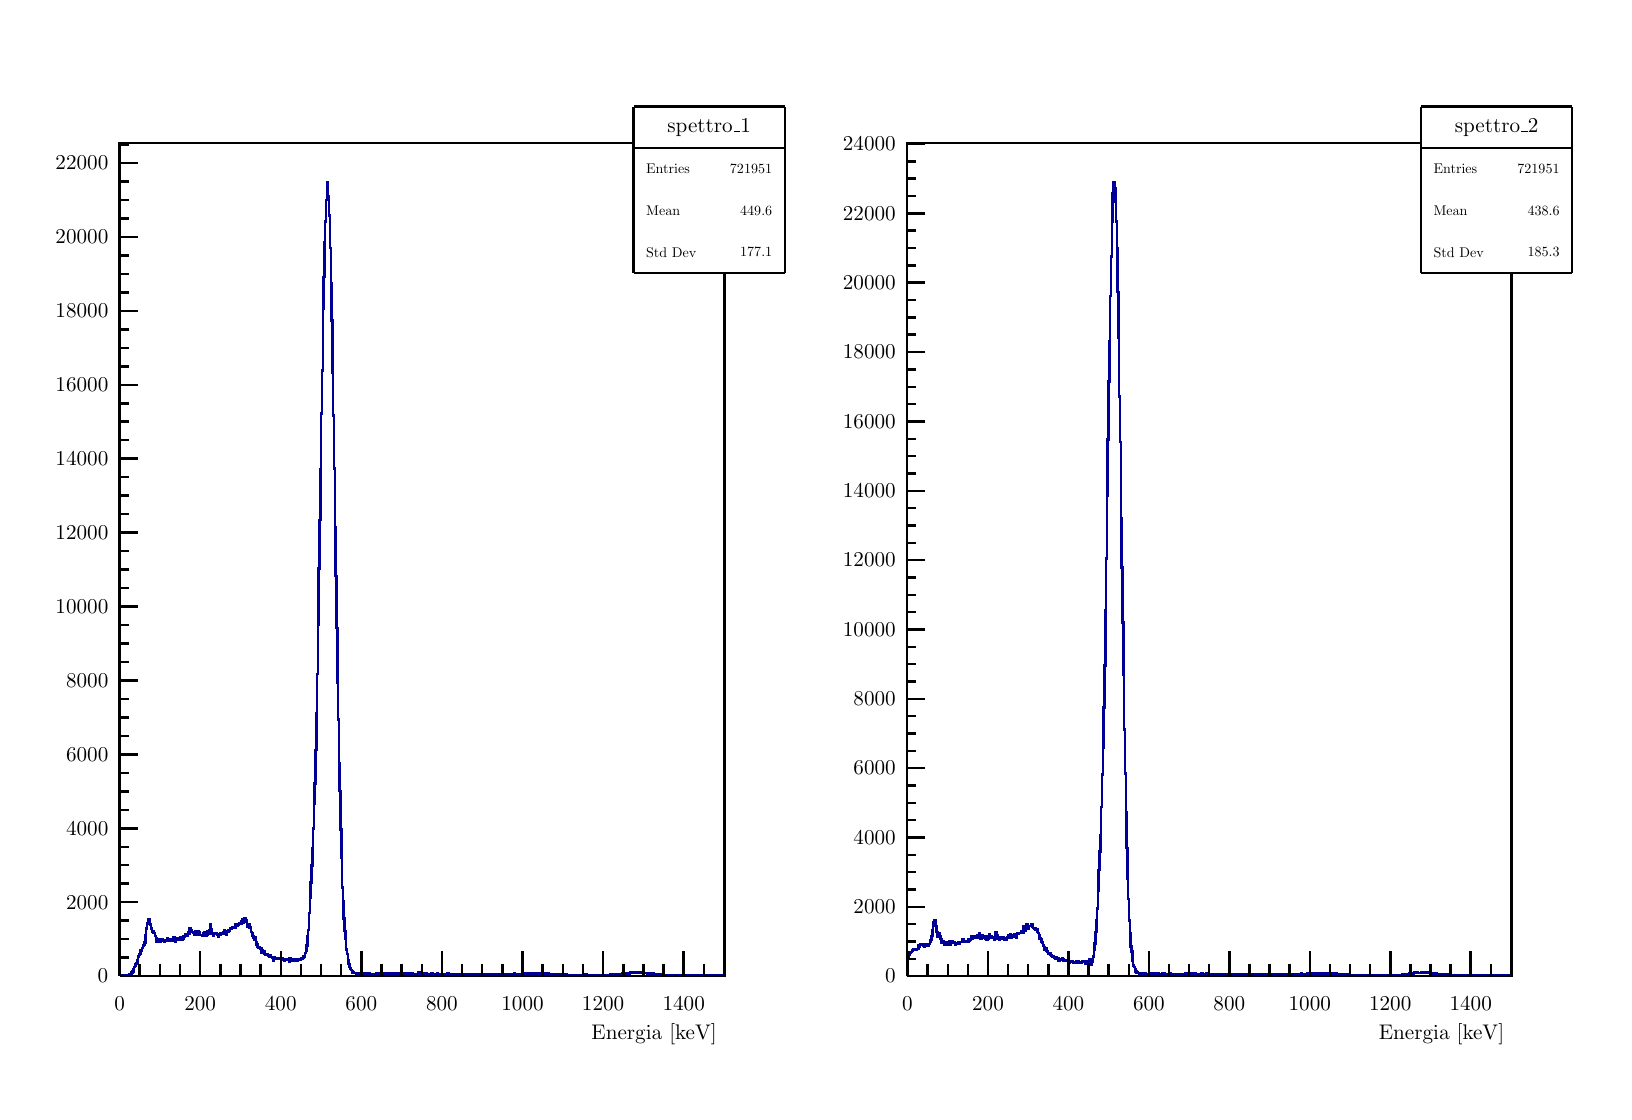
\begin{tikzpicture}
\pgfdeclareplotmark{cross} {
\pgfpathmoveto{\pgfpoint{-0.3\pgfplotmarksize}{\pgfplotmarksize}}
\pgfpathlineto{\pgfpoint{+0.3\pgfplotmarksize}{\pgfplotmarksize}}
\pgfpathlineto{\pgfpoint{+0.3\pgfplotmarksize}{0.3\pgfplotmarksize}}
\pgfpathlineto{\pgfpoint{+1\pgfplotmarksize}{0.3\pgfplotmarksize}}
\pgfpathlineto{\pgfpoint{+1\pgfplotmarksize}{-0.3\pgfplotmarksize}}
\pgfpathlineto{\pgfpoint{+0.3\pgfplotmarksize}{-0.3\pgfplotmarksize}}
\pgfpathlineto{\pgfpoint{+0.3\pgfplotmarksize}{-1.\pgfplotmarksize}}
\pgfpathlineto{\pgfpoint{-0.3\pgfplotmarksize}{-1.\pgfplotmarksize}}
\pgfpathlineto{\pgfpoint{-0.3\pgfplotmarksize}{-0.3\pgfplotmarksize}}
\pgfpathlineto{\pgfpoint{-1.\pgfplotmarksize}{-0.3\pgfplotmarksize}}
\pgfpathlineto{\pgfpoint{-1.\pgfplotmarksize}{0.3\pgfplotmarksize}}
\pgfpathlineto{\pgfpoint{-0.3\pgfplotmarksize}{0.3\pgfplotmarksize}}
\pgfpathclose
\pgfusepathqstroke
}
\pgfdeclareplotmark{cross*} {
\pgfpathmoveto{\pgfpoint{-0.3\pgfplotmarksize}{\pgfplotmarksize}}
\pgfpathlineto{\pgfpoint{+0.3\pgfplotmarksize}{\pgfplotmarksize}}
\pgfpathlineto{\pgfpoint{+0.3\pgfplotmarksize}{0.3\pgfplotmarksize}}
\pgfpathlineto{\pgfpoint{+1\pgfplotmarksize}{0.3\pgfplotmarksize}}
\pgfpathlineto{\pgfpoint{+1\pgfplotmarksize}{-0.3\pgfplotmarksize}}
\pgfpathlineto{\pgfpoint{+0.3\pgfplotmarksize}{-0.3\pgfplotmarksize}}
\pgfpathlineto{\pgfpoint{+0.3\pgfplotmarksize}{-1.\pgfplotmarksize}}
\pgfpathlineto{\pgfpoint{-0.3\pgfplotmarksize}{-1.\pgfplotmarksize}}
\pgfpathlineto{\pgfpoint{-0.3\pgfplotmarksize}{-0.3\pgfplotmarksize}}
\pgfpathlineto{\pgfpoint{-1.\pgfplotmarksize}{-0.3\pgfplotmarksize}}
\pgfpathlineto{\pgfpoint{-1.\pgfplotmarksize}{0.3\pgfplotmarksize}}
\pgfpathlineto{\pgfpoint{-0.3\pgfplotmarksize}{0.3\pgfplotmarksize}}
\pgfpathclose
\pgfusepathqfillstroke
}
\pgfdeclareplotmark{newstar} {
\pgfpathmoveto{\pgfqpoint{0pt}{\pgfplotmarksize}}
\pgfpathlineto{\pgfqpointpolar{44}{0.5\pgfplotmarksize}}
\pgfpathlineto{\pgfqpointpolar{18}{\pgfplotmarksize}}
\pgfpathlineto{\pgfqpointpolar{-20}{0.5\pgfplotmarksize}}
\pgfpathlineto{\pgfqpointpolar{-54}{\pgfplotmarksize}}
\pgfpathlineto{\pgfqpointpolar{-90}{0.5\pgfplotmarksize}}
\pgfpathlineto{\pgfqpointpolar{234}{\pgfplotmarksize}}
\pgfpathlineto{\pgfqpointpolar{198}{0.5\pgfplotmarksize}}
\pgfpathlineto{\pgfqpointpolar{162}{\pgfplotmarksize}}
\pgfpathlineto{\pgfqpointpolar{134}{0.5\pgfplotmarksize}}
\pgfpathclose
\pgfusepathqstroke
}
\pgfdeclareplotmark{newstar*} {
\pgfpathmoveto{\pgfqpoint{0pt}{\pgfplotmarksize}}
\pgfpathlineto{\pgfqpointpolar{44}{0.5\pgfplotmarksize}}
\pgfpathlineto{\pgfqpointpolar{18}{\pgfplotmarksize}}
\pgfpathlineto{\pgfqpointpolar{-20}{0.5\pgfplotmarksize}}
\pgfpathlineto{\pgfqpointpolar{-54}{\pgfplotmarksize}}
\pgfpathlineto{\pgfqpointpolar{-90}{0.5\pgfplotmarksize}}
\pgfpathlineto{\pgfqpointpolar{234}{\pgfplotmarksize}}
\pgfpathlineto{\pgfqpointpolar{198}{0.5\pgfplotmarksize}}
\pgfpathlineto{\pgfqpointpolar{162}{\pgfplotmarksize}}
\pgfpathlineto{\pgfqpointpolar{134}{0.5\pgfplotmarksize}}
\pgfpathclose
\pgfusepathqfillstroke
}
\definecolor{c}{rgb}{1,1,1};
\draw [color=c, fill=c] (0,0) rectangle (20,13.4957);
\draw [color=c, fill=c] (0.2,0.134957) rectangle (9.8,13.3607);
\draw [color=c, fill=c] (1.16,1.45754) rectangle (8.84,12.0382);
\definecolor{c}{rgb}{0,0,0};
\draw [c,line width=0.9] (1.16,1.45754) -- (1.16,12.0382) -- (8.84,12.0382) -- (8.84,1.45754) -- (1.16,1.45754);
\definecolor{c}{rgb}{1,1,1};
\draw [color=c, fill=c] (1.16,1.45754) rectangle (8.84,12.0382);
\definecolor{c}{rgb}{0,0,0};
\draw [c,line width=0.9] (1.16,1.45754) -- (1.16,12.0382) -- (8.84,12.0382) -- (8.84,1.45754) -- (1.16,1.45754);
\definecolor{c}{rgb}{0,0,0.6};
\draw [c,line width=0.9] (1.16,1.47162) -- (1.17024,1.47162) -- (1.17024,1.47209) -- (1.18048,1.47209) -- (1.18048,1.46786) -- (1.19072,1.46786) -- (1.19072,1.47209) -- (1.20096,1.47209) -- (1.20096,1.47349) -- (1.2112,1.47349) -- (1.2112,1.46927) --
 (1.22144,1.46927) -- (1.22144,1.46739) -- (1.23168,1.46739) -- (1.23168,1.47396) -- (1.24192,1.47396) -- (1.24192,1.4688) -- (1.25216,1.4688) -- (1.25216,1.47021) -- (1.2624,1.47021) -- (1.2624,1.47396) -- (1.27264,1.47396) -- (1.27264,1.47349) --
 (1.28288,1.47349) -- (1.28288,1.47819) -- (1.29312,1.47819) -- (1.29312,1.48617) -- (1.30336,1.48617) -- (1.30336,1.49227) -- (1.3136,1.49227) -- (1.3136,1.50635) -- (1.32384,1.50635) -- (1.32384,1.51621) -- (1.33408,1.51621) -- (1.33408,1.55047) --
 (1.34432,1.55047) -- (1.34432,1.57159) -- (1.35456,1.57159) -- (1.35456,1.58567) -- (1.3648,1.58567) -- (1.3648,1.60914) -- (1.37504,1.60914) -- (1.37504,1.62134) -- (1.38528,1.62134) -- (1.38528,1.6603) -- (1.39552,1.6603) -- (1.39552,1.70818) --
 (1.40576,1.70818) -- (1.40576,1.72414) -- (1.416,1.72414) -- (1.416,1.74103) -- (1.42624,1.74103) -- (1.42624,1.78515) -- (1.43648,1.78515) -- (1.43648,1.78515) -- (1.44672,1.78515) -- (1.44672,1.8166) -- (1.45696,1.8166) -- (1.45696,1.84382) --
 (1.4672,1.84382) -- (1.4672,1.85509) -- (1.47744,1.85509) -- (1.47744,1.88325) -- (1.48768,1.88325) -- (1.48768,1.97994) -- (1.49792,1.97994) -- (1.49792,2.06114) -- (1.50816,2.06114) -- (1.50816,2.12263) -- (1.5184,2.12263) -- (1.5184,2.18552) --
 (1.52864,2.18552) -- (1.52864,2.17895) -- (1.53888,2.17895) -- (1.53888,2.16252) -- (1.54912,2.16252) -- (1.54912,2.11136) -- (1.55936,2.11136) -- (1.55936,2.06302) -- (1.5696,2.06302) -- (1.5696,2.02641) -- (1.57984,2.02641) -- (1.57984,2.02734) --
 (1.59008,2.02734) -- (1.59008,2.00669) -- (1.60032,2.00669) -- (1.60032,2.00669) -- (1.61056,2.00669) -- (1.61056,1.9668) -- (1.6208,1.9668) -- (1.6208,1.9438) -- (1.63104,1.9438) -- (1.63104,1.89921) -- (1.64128,1.89921) -- (1.64128,1.92033) --
 (1.65152,1.92033) -- (1.65152,1.9086) -- (1.66176,1.9086) -- (1.66176,1.91235) -- (1.672,1.91235) -- (1.672,1.89639) -- (1.68224,1.89639) -- (1.68224,1.92549) -- (1.69248,1.92549) -- (1.69248,1.9269) -- (1.70272,1.9269) -- (1.70272,1.90766) --
 (1.71296,1.90766) -- (1.71296,1.91047) -- (1.7232,1.91047) -- (1.7232,1.88888) -- (1.73344,1.88888) -- (1.73344,1.90766) -- (1.74368,1.90766) -- (1.74368,1.91892) -- (1.75392,1.91892) -- (1.75392,1.91188) -- (1.76416,1.91188) -- (1.76416,1.93441) --
 (1.7744,1.93441) -- (1.7744,1.93206) -- (1.78464,1.93206) -- (1.78464,1.92033) -- (1.79488,1.92033) -- (1.79488,1.91) -- (1.80512,1.91) -- (1.80512,1.92268) -- (1.81536,1.92268) -- (1.81536,1.92878) -- (1.8256,1.92878) -- (1.8256,1.91188) --
 (1.83584,1.91188) -- (1.83584,1.90202) -- (1.84608,1.90202) -- (1.84608,1.94521) -- (1.85632,1.94521) -- (1.85632,1.91657) -- (1.86656,1.91657) -- (1.86656,1.89921) -- (1.8768,1.89921) -- (1.8768,1.93676) -- (1.88704,1.93676) -- (1.88704,1.93347) --
 (1.89728,1.93347) -- (1.89728,1.91939) -- (1.90752,1.91939) -- (1.90752,1.91986) -- (1.91776,1.91986) -- (1.91776,1.93723) -- (1.928,1.93723) -- (1.928,1.95459) -- (1.93824,1.95459) -- (1.93824,1.94568) -- (1.94848,1.94568) -- (1.94848,1.91423) --
 (1.95872,1.91423) -- (1.95872,1.93159) -- (1.96896,1.93159) -- (1.96896,1.97008) -- (1.9792,1.97008) -- (1.9792,1.95553) -- (1.98944,1.95553) -- (1.98944,1.97384) -- (1.99968,1.97384) -- (1.99968,1.98604) -- (2.00992,1.98604) -- (2.00992,1.98041) --
 (2.02016,1.98041) -- (2.02016,1.97525) -- (2.0304,1.97525) -- (2.0304,2.01467) -- (2.04064,2.01467) -- (2.04064,1.99543) -- (2.05088,1.99543) -- (2.05088,2.06161) -- (2.06112,2.06161) -- (2.06112,2.03016) -- (2.07136,2.03016) -- (2.07136,2.0433) --
 (2.0816,2.0433) -- (2.0816,2.01796) -- (2.09184,2.01796) -- (2.09184,2.00294) -- (2.10208,2.00294) -- (2.10208,2.00716) -- (2.11232,2.00716) -- (2.11232,1.98088) -- (2.12256,1.98088) -- (2.12256,2.02265) -- (2.1328,2.02265) -- (2.1328,2.00106) --
 (2.14304,2.00106) -- (2.14304,1.98416) -- (2.15328,1.98416) -- (2.15328,2.02453) -- (2.16352,2.02453) -- (2.16352,1.98698) -- (2.17376,1.98698) -- (2.17376,2.01279) -- (2.184,2.01279) -- (2.184,1.98135) -- (2.19424,1.98135) -- (2.19424,1.979) --
 (2.20448,1.979) -- (2.20448,1.98041) -- (2.21472,1.98041) -- (2.21472,1.96961) -- (2.22496,1.96961) -- (2.22496,1.99684) -- (2.2352,1.99684) -- (2.2352,2.01186) -- (2.24544,2.01186) -- (2.24544,1.98651) -- (2.25568,1.98651) -- (2.25568,1.96398) --
 (2.26592,1.96398) -- (2.26592,1.98651) -- (2.27616,1.98651) -- (2.27616,2.03016) -- (2.2864,2.03016) -- (2.2864,1.99731) -- (2.29664,1.99731) -- (2.29664,2.03532) -- (2.30688,2.03532) -- (2.30688,2.1123) -- (2.31712,2.1123) -- (2.31712,2.04706) --
 (2.32736,2.04706) -- (2.32736,1.9959) -- (2.3376,1.9959) -- (2.3376,2.00388) -- (2.34784,2.00388) -- (2.34784,1.97571) -- (2.35808,1.97571) -- (2.35808,2.00669) -- (2.36832,2.00669) -- (2.36832,2.00482) -- (2.37856,2.00482) -- (2.37856,1.99402) --
 (2.3888,1.99402) -- (2.3888,2.00294) -- (2.39904,2.00294) -- (2.39904,1.97806) -- (2.40928,1.97806) -- (2.40928,1.96351) -- (2.41952,1.96351) -- (2.41952,1.98604) -- (2.42976,1.98604) -- (2.42976,1.97806) -- (2.44,1.97806) -- (2.44,2.00012) --
 (2.45024,2.00012) -- (2.45024,1.9912) -- (2.46048,1.9912) -- (2.46048,1.99308) -- (2.47072,1.99308) -- (2.47072,2.01139) -- (2.48096,2.01139) -- (2.48096,2.00153) -- (2.4912,2.00153) -- (2.4912,2.03767) -- (2.50144,2.03767) -- (2.50144,2.025) --
 (2.51168,2.025) -- (2.51168,1.98463) -- (2.52192,1.98463) -- (2.52192,2.02265) -- (2.53216,2.02265) -- (2.53216,2.01937) -- (2.5424,2.01937) -- (2.5424,2.03861) -- (2.55264,2.03861) -- (2.55264,2.03157) -- (2.56288,2.03157) -- (2.56288,2.06818) --
 (2.57312,2.06818) -- (2.57312,2.06396) -- (2.58336,2.06396) -- (2.58336,2.06724) -- (2.5936,2.06724) -- (2.5936,2.07381) -- (2.60384,2.07381) -- (2.60384,2.07428) -- (2.61408,2.07428) -- (2.61408,2.06912) -- (2.62432,2.06912) -- (2.62432,2.07663) --
 (2.63456,2.07663) -- (2.63456,2.12216) -- (2.6448,2.12216) -- (2.6448,2.11699) -- (2.65504,2.11699) -- (2.65504,2.09963) -- (2.66528,2.09963) -- (2.66528,2.11324) -- (2.67552,2.11324) -- (2.67552,2.1292) -- (2.68576,2.1292) -- (2.68576,2.13483) --
 (2.696,2.13483) -- (2.696,2.12075) -- (2.70624,2.12075) -- (2.70624,2.1522) -- (2.71648,2.1522) -- (2.71648,2.17379) -- (2.72672,2.17379) -- (2.72672,2.13905) -- (2.73696,2.13905) -- (2.73696,2.14891) -- (2.7472,2.14891) -- (2.7472,2.19585) --
 (2.75744,2.19585) -- (2.75744,2.17801) -- (2.76768,2.17801) -- (2.76768,2.16346) -- (2.77792,2.16346) -- (2.77792,2.08555) -- (2.78816,2.08555) -- (2.78816,2.09071) -- (2.7984,2.09071) -- (2.7984,2.11605) -- (2.80864,2.11605) -- (2.80864,2.07334) --
 (2.81888,2.07334) -- (2.81888,2.07569) -- (2.82912,2.07569) -- (2.82912,2.01702) -- (2.83936,2.01702) -- (2.83936,2.00388) -- (2.8496,2.00388) -- (2.8496,1.96867) -- (2.85984,1.96867) -- (2.85984,1.95084) -- (2.87008,1.95084) -- (2.87008,1.91986) --
 (2.88032,1.91986) -- (2.88032,1.94849) -- (2.89056,1.94849) -- (2.89056,1.88137) -- (2.9008,1.88137) -- (2.9008,1.85931) -- (2.91104,1.85931) -- (2.91104,1.83444) -- (2.92128,1.83444) -- (2.92128,1.81425) -- (2.93152,1.81425) -- (2.93152,1.83021) --
 (2.94176,1.83021) -- (2.94176,1.80158) -- (2.952,1.80158) -- (2.952,1.80627) -- (2.96224,1.80627) -- (2.96224,1.75887) -- (2.97248,1.75887) -- (2.97248,1.78985) -- (2.98272,1.78985) -- (2.98272,1.75136) -- (2.99296,1.75136) -- (2.99296,1.76732) --
 (3.0032,1.76732) -- (3.0032,1.7415) -- (3.01344,1.7415) -- (3.01344,1.73352) -- (3.02368,1.73352) -- (3.02368,1.73728) -- (3.03392,1.73728) -- (3.03392,1.72977) -- (3.04416,1.72977) -- (3.04416,1.71756) -- (3.0544,1.71756) -- (3.0544,1.71193) --
 (3.06464,1.71193) -- (3.06464,1.7063) -- (3.07488,1.7063) -- (3.07488,1.71803) -- (3.08512,1.71803) -- (3.08512,1.69785) -- (3.09536,1.69785) -- (3.09536,1.6941) -- (3.1056,1.6941) -- (3.1056,1.65608) -- (3.11584,1.65608) -- (3.11584,1.6941) --
 (3.12608,1.6941) -- (3.12608,1.69316) -- (3.13632,1.69316) -- (3.13632,1.6833) -- (3.14656,1.6833) -- (3.14656,1.68001) -- (3.1568,1.68001) -- (3.1568,1.6833) -- (3.16704,1.6833) -- (3.16704,1.68893) -- (3.17728,1.68893) -- (3.17728,1.67955) --
 (3.18752,1.67955) -- (3.18752,1.69034) -- (3.19776,1.69034) -- (3.19776,1.67297) -- (3.208,1.67297) -- (3.208,1.66875) -- (3.21824,1.66875) -- (3.21824,1.665) -- (3.22848,1.665) -- (3.22848,1.68471) -- (3.23872,1.68471) -- (3.23872,1.66546) --
 (3.24896,1.66546) -- (3.24896,1.65842) -- (3.2592,1.65842) -- (3.2592,1.66359) -- (3.26944,1.66359) -- (3.26944,1.66218) -- (3.27968,1.66218) -- (3.27968,1.67673) -- (3.28992,1.67673) -- (3.28992,1.6772) -- (3.30016,1.6772) -- (3.30016,1.6772) --
 (3.3104,1.6772) -- (3.3104,1.64293) -- (3.32064,1.64293) -- (3.32064,1.67908) -- (3.33088,1.67908) -- (3.33088,1.67579) -- (3.34112,1.67579) -- (3.34112,1.66922) -- (3.35136,1.66922) -- (3.35136,1.64998) -- (3.3616,1.64998) -- (3.3616,1.66875) --
 (3.37184,1.66875) -- (3.37184,1.66922) -- (3.38208,1.66922) -- (3.38208,1.65373) -- (3.39232,1.65373) -- (3.39232,1.65608) -- (3.40256,1.65608) -- (3.40256,1.67438) -- (3.4128,1.67438) -- (3.4128,1.65373) -- (3.42304,1.65373) -- (3.42304,1.66969) --
 (3.43328,1.66969) -- (3.43328,1.66124) -- (3.44352,1.66124) -- (3.44352,1.665) -- (3.45376,1.665) -- (3.45376,1.67157) -- (3.464,1.67157) -- (3.464,1.67908) -- (3.47424,1.67908) -- (3.47424,1.6833) -- (3.48448,1.6833) -- (3.48448,1.68612) --
 (3.49472,1.68612) -- (3.49472,1.71616) -- (3.50496,1.71616) -- (3.50496,1.70114) -- (3.5152,1.70114) -- (3.5152,1.75183) -- (3.52544,1.75183) -- (3.52544,1.78515) -- (3.53568,1.78515) -- (3.53568,1.84523) -- (3.54592,1.84523) -- (3.54592,1.9621) --
 (3.55616,1.9621) -- (3.55616,2.04002) -- (3.5664,2.04002) -- (3.5664,2.25827) -- (3.57664,2.25827) -- (3.57664,2.44743) -- (3.58688,2.44743) -- (3.58688,2.64362) -- (3.59712,2.64362) -- (3.59712,2.86094) -- (3.60736,2.86094) -- (3.60736,3.07637) --
 (3.6176,3.07637) -- (3.6176,3.33453) -- (3.62784,3.33453) -- (3.62784,3.64853) -- (3.63808,3.64853) -- (3.63808,3.90574) -- (3.64832,3.90574) -- (3.64832,4.32911) -- (3.65856,4.32911) -- (3.65856,4.79378) -- (3.6688,4.79378) -- (3.6688,5.29365) --
 (3.67904,5.29365) -- (3.67904,5.91415) -- (3.68928,5.91415) -- (3.68928,6.63134) -- (3.69952,6.63134) -- (3.69952,7.2495) -- (3.70976,7.2495) -- (3.70976,7.89487) -- (3.72,7.89487) -- (3.72,8.60314) -- (3.73024,8.60314) -- (3.73024,9.1462) --
 (3.74048,9.1462) -- (3.74048,9.92675) -- (3.75072,9.92675) -- (3.75072,10.3337) -- (3.76096,10.3337) -- (3.76096,10.7829) -- (3.7712,10.7829) -- (3.7712,11.041) -- (3.78144,11.041) -- (3.78144,11.3133) -- (3.79168,11.3133) -- (3.79168,11.5343) --
 (3.80192,11.5343) -- (3.80192,11.3372) -- (3.81216,11.3372) -- (3.81216,11.356) -- (3.8224,11.356) -- (3.8224,11.1152) -- (3.83264,11.1152) -- (3.83264,10.7059) -- (3.84288,10.7059) -- (3.84288,10.2506) -- (3.85312,10.2506) -- (3.85312,9.78172) --
 (3.86336,9.78172) -- (3.86336,9.11616) -- (3.8736,9.11616) -- (3.8736,8.5778) -- (3.88384,8.5778) -- (3.88384,7.90285) -- (3.89408,7.90285) -- (3.89408,7.15375) -- (3.90432,7.15375) -- (3.90432,6.53982) -- (3.91456,6.53982) -- (3.91456,5.8766) --
 (3.9248,5.8766) -- (3.9248,5.18758) -- (3.93504,5.18758) -- (3.93504,4.71399) -- (3.94528,4.71399) -- (3.94528,4.15591) -- (3.95552,4.15591) -- (3.95552,3.80999) -- (3.96576,3.80999) -- (3.96576,3.31857) -- (3.976,3.31857) -- (3.976,2.96044) --
 (3.98624,2.96044) -- (3.98624,2.58401) -- (3.99648,2.58401) -- (3.99648,2.41316) -- (4.00672,2.41316) -- (4.00672,2.19209) -- (4.01696,2.19209) -- (4.01696,2.03345) -- (4.0272,2.03345) -- (4.0272,1.93676) -- (4.03744,1.93676) -- (4.03744,1.79313) --
 (4.04768,1.79313) -- (4.04768,1.73681) -- (4.05792,1.73681) -- (4.05792,1.665) -- (4.06816,1.665) -- (4.06816,1.60961) -- (4.0784,1.60961) -- (4.0784,1.57441) -- (4.08864,1.57441) -- (4.08864,1.55329) -- (4.09888,1.55329) -- (4.09888,1.53686) --
 (4.10912,1.53686) -- (4.10912,1.52372) -- (4.11936,1.52372) -- (4.11936,1.50588) -- (4.1296,1.50588) -- (4.1296,1.50823) -- (4.13984,1.50823) -- (4.13984,1.49602) -- (4.15008,1.49602) -- (4.15008,1.4979) -- (4.16032,1.4979) -- (4.16032,1.49321) --
 (4.17056,1.49321) -- (4.17056,1.49462) -- (4.1808,1.49462) -- (4.1808,1.48476) -- (4.19104,1.48476) -- (4.19104,1.48664) -- (4.20128,1.48664) -- (4.20128,1.49555) -- (4.21152,1.49555) -- (4.21152,1.49837) -- (4.22176,1.49837) -- (4.22176,1.49462) --
 (4.232,1.49462) -- (4.232,1.48945) -- (4.24224,1.48945) -- (4.24224,1.49274) -- (4.25248,1.49274) -- (4.25248,1.49649) -- (4.26272,1.49649) -- (4.26272,1.48851) -- (4.27296,1.48851) -- (4.27296,1.49509) -- (4.2832,1.49509) -- (4.2832,1.48898) --
 (4.29344,1.48898) -- (4.29344,1.4857) -- (4.30368,1.4857) -- (4.30368,1.49039) -- (4.31392,1.49039) -- (4.31392,1.49602) -- (4.32416,1.49602) -- (4.32416,1.49039) -- (4.3344,1.49039) -- (4.3344,1.4857) -- (4.34464,1.4857) -- (4.34464,1.48429) --
 (4.35488,1.48429) -- (4.35488,1.48664) -- (4.36512,1.48664) -- (4.36512,1.48711) -- (4.37536,1.48711) -- (4.37536,1.48288) -- (4.3856,1.48288) -- (4.3856,1.48382) -- (4.39584,1.48382) -- (4.39584,1.48382) -- (4.40608,1.48382) -- (4.40608,1.48194) --
 (4.41632,1.48194) -- (4.41632,1.48898) -- (4.42656,1.48898) -- (4.42656,1.48335) -- (4.4368,1.48335) -- (4.4368,1.48288) -- (4.44704,1.48288) -- (4.44704,1.48053) -- (4.45728,1.48053) -- (4.45728,1.48992) -- (4.46752,1.48992) -- (4.46752,1.48664) --
 (4.47776,1.48664) -- (4.47776,1.49321) -- (4.488,1.49321) -- (4.488,1.49133) -- (4.49824,1.49133) -- (4.49824,1.48523) -- (4.50848,1.48523) -- (4.50848,1.49039) -- (4.51872,1.49039) -- (4.51872,1.48523) -- (4.52896,1.48523) -- (4.52896,1.48429) --
 (4.5392,1.48429) -- (4.5392,1.48804) -- (4.54944,1.48804) -- (4.54944,1.48992) -- (4.55968,1.48992) -- (4.55968,1.48945) -- (4.56992,1.48945) -- (4.56992,1.48898) -- (4.58016,1.48898) -- (4.58016,1.48898) -- (4.5904,1.48898) -- (4.5904,1.48898) --
 (4.60064,1.48898) -- (4.60064,1.48851) -- (4.61088,1.48851) -- (4.61088,1.49415) -- (4.62112,1.49415) -- (4.62112,1.48664) -- (4.63136,1.48664) -- (4.63136,1.48382) -- (4.6416,1.48382) -- (4.6416,1.48007) -- (4.65184,1.48007) -- (4.65184,1.49227) --
 (4.66208,1.49227) -- (4.66208,1.48664) -- (4.67232,1.48664) -- (4.67232,1.48617) -- (4.68256,1.48617) -- (4.68256,1.48335) -- (4.6928,1.48335) -- (4.6928,1.48945) -- (4.70304,1.48945) -- (4.70304,1.49368) -- (4.71328,1.49368) -- (4.71328,1.48523) --
 (4.72352,1.48523) -- (4.72352,1.49321) -- (4.73376,1.49321) -- (4.73376,1.48758) -- (4.744,1.48758) -- (4.744,1.49274) -- (4.75424,1.49274) -- (4.75424,1.48382) -- (4.76448,1.48382) -- (4.76448,1.48523) -- (4.77472,1.48523) -- (4.77472,1.49039) --
 (4.78496,1.49039) -- (4.78496,1.48898) -- (4.7952,1.48898) -- (4.7952,1.49039) -- (4.80544,1.49039) -- (4.80544,1.48851) -- (4.81568,1.48851) -- (4.81568,1.49696) -- (4.82592,1.49696) -- (4.82592,1.49696) -- (4.83616,1.49696) -- (4.83616,1.48758) --
 (4.8464,1.48758) -- (4.8464,1.48992) -- (4.85664,1.48992) -- (4.85664,1.48758) -- (4.86688,1.48758) -- (4.86688,1.47866) -- (4.87712,1.47866) -- (4.87712,1.49462) -- (4.88736,1.49462) -- (4.88736,1.48758) -- (4.8976,1.48758) -- (4.8976,1.48523) --
 (4.90784,1.48523) -- (4.90784,1.48476) -- (4.91808,1.48476) -- (4.91808,1.48711) -- (4.92832,1.48711) -- (4.92832,1.48382) -- (4.93856,1.48382) -- (4.93856,1.48523) -- (4.9488,1.48523) -- (4.9488,1.49415) -- (4.95904,1.49415) -- (4.95904,1.50072) --
 (4.96928,1.50072) -- (4.96928,1.481) -- (4.97952,1.481) -- (4.97952,1.4918) -- (4.98976,1.4918) -- (4.98976,1.48476) -- (5,1.48476) -- (5,1.4796) -- (5.01024,1.4796) -- (5.01024,1.48194) -- (5.02048,1.48194) -- (5.02048,1.48992) -- (5.03072,1.48992)
 -- (5.03072,1.481) -- (5.04096,1.481) -- (5.04096,1.48335) -- (5.0512,1.48335) -- (5.0512,1.49227) -- (5.06144,1.49227) -- (5.06144,1.48382) -- (5.07168,1.48382) -- (5.07168,1.48288) -- (5.08192,1.48288) -- (5.08192,1.48194) -- (5.09216,1.48194) --
 (5.09216,1.48523) -- (5.1024,1.48523) -- (5.1024,1.48288) -- (5.11264,1.48288) -- (5.11264,1.47819) -- (5.12288,1.47819) -- (5.12288,1.48804) -- (5.13312,1.48804) -- (5.13312,1.48804) -- (5.14336,1.48804) -- (5.14336,1.48664) -- (5.1536,1.48664) --
 (5.1536,1.48711) -- (5.16384,1.48711) -- (5.16384,1.481) -- (5.17408,1.481) -- (5.17408,1.48288) -- (5.18432,1.48288) -- (5.18432,1.48288) -- (5.19456,1.48288) -- (5.19456,1.48945) -- (5.2048,1.48945) -- (5.2048,1.48476) -- (5.21504,1.48476) --
 (5.21504,1.48758) -- (5.22528,1.48758) -- (5.22528,1.4796) -- (5.23552,1.4796) -- (5.23552,1.48758) -- (5.24576,1.48758) -- (5.24576,1.48711) -- (5.256,1.48711) -- (5.256,1.48523) -- (5.26624,1.48523) -- (5.26624,1.48429) -- (5.27648,1.48429) --
 (5.27648,1.48241) -- (5.28672,1.48241) -- (5.28672,1.481) -- (5.29696,1.481) -- (5.29696,1.48711) -- (5.3072,1.48711) -- (5.3072,1.48476) -- (5.31744,1.48476) -- (5.31744,1.48007) -- (5.32768,1.48007) -- (5.32768,1.48804) -- (5.33792,1.48804) --
 (5.33792,1.48664) -- (5.34816,1.48664) -- (5.34816,1.4796) -- (5.3584,1.4796) -- (5.3584,1.48664) -- (5.36864,1.48664) -- (5.36864,1.47584) -- (5.37888,1.47584) -- (5.37888,1.47725) -- (5.38912,1.47725) -- (5.38912,1.47866) -- (5.39936,1.47866) --
 (5.39936,1.4857) -- (5.4096,1.4857) -- (5.4096,1.47772) -- (5.41984,1.47772) -- (5.41984,1.48288) -- (5.43008,1.48288) -- (5.43008,1.4796) -- (5.44032,1.4796) -- (5.44032,1.48523) -- (5.45056,1.48523) -- (5.45056,1.48476) -- (5.4608,1.48476) --
 (5.4608,1.48147) -- (5.47104,1.48147) -- (5.47104,1.47819) -- (5.48128,1.47819) -- (5.48128,1.47913) -- (5.49152,1.47913) -- (5.49152,1.48429) -- (5.50176,1.48429) -- (5.50176,1.48194) -- (5.512,1.48194) -- (5.512,1.47819) -- (5.52224,1.47819) --
 (5.52224,1.48194) -- (5.53248,1.48194) -- (5.53248,1.4796) -- (5.54272,1.4796) -- (5.54272,1.47725) -- (5.55296,1.47725) -- (5.55296,1.4796) -- (5.5632,1.4796) -- (5.5632,1.47678) -- (5.57344,1.47678) -- (5.57344,1.48288) -- (5.58368,1.48288) --
 (5.58368,1.47772) -- (5.59392,1.47772) -- (5.59392,1.47584) -- (5.60416,1.47584) -- (5.60416,1.47725) -- (5.6144,1.47725) -- (5.6144,1.47772) -- (5.62464,1.47772) -- (5.62464,1.4796) -- (5.63488,1.4796) -- (5.63488,1.4749) -- (5.64512,1.4749) --
 (5.64512,1.47913) -- (5.65536,1.47913) -- (5.65536,1.47725) -- (5.6656,1.47725) -- (5.6656,1.47772) -- (5.67584,1.47772) -- (5.67584,1.48007) -- (5.68608,1.48007) -- (5.68608,1.481) -- (5.69632,1.481) -- (5.69632,1.47913) -- (5.70656,1.47913) --
 (5.70656,1.47302) -- (5.7168,1.47302) -- (5.7168,1.481) -- (5.72704,1.481) -- (5.72704,1.4796) -- (5.73728,1.4796) -- (5.73728,1.48523) -- (5.74752,1.48523) -- (5.74752,1.47866) -- (5.75776,1.47866) -- (5.75776,1.47349) -- (5.768,1.47349) --
 (5.768,1.47725) -- (5.77824,1.47725) -- (5.77824,1.48382) -- (5.78848,1.48382) -- (5.78848,1.48147) -- (5.79872,1.48147) -- (5.79872,1.48007) -- (5.80896,1.48007) -- (5.80896,1.47913) -- (5.8192,1.47913) -- (5.8192,1.4796) -- (5.82944,1.4796) --
 (5.82944,1.481) -- (5.83968,1.481) -- (5.83968,1.47537) -- (5.84992,1.47537) -- (5.84992,1.48147) -- (5.86016,1.48147) -- (5.86016,1.48147) -- (5.8704,1.48147) -- (5.8704,1.48241) -- (5.88064,1.48241) -- (5.88064,1.47725) -- (5.89088,1.47725) --
 (5.89088,1.47725) -- (5.90112,1.47725) -- (5.90112,1.47725) -- (5.91136,1.47725) -- (5.91136,1.48147) -- (5.9216,1.48147) -- (5.9216,1.47631) -- (5.93184,1.47631) -- (5.93184,1.47913) -- (5.94208,1.47913) -- (5.94208,1.47866) -- (5.95232,1.47866) --
 (5.95232,1.4796) -- (5.96256,1.4796) -- (5.96256,1.48617) -- (5.9728,1.48617) -- (5.9728,1.4796) -- (5.98304,1.4796) -- (5.98304,1.48053) -- (5.99328,1.48053) -- (5.99328,1.47866) -- (6.00352,1.47866) -- (6.00352,1.48007) -- (6.01376,1.48007) --
 (6.01376,1.48288) -- (6.024,1.48288) -- (6.024,1.48335) -- (6.03424,1.48335) -- (6.03424,1.47866) -- (6.04448,1.47866) -- (6.04448,1.48382) -- (6.05472,1.48382) -- (6.05472,1.47678) -- (6.06496,1.47678) -- (6.06496,1.48335) -- (6.0752,1.48335) --
 (6.0752,1.48523) -- (6.08544,1.48523) -- (6.08544,1.48194) -- (6.09568,1.48194) -- (6.09568,1.48194) -- (6.10592,1.48194) -- (6.10592,1.48288) -- (6.11616,1.48288) -- (6.11616,1.48382) -- (6.1264,1.48382) -- (6.1264,1.4857) -- (6.13664,1.4857) --
 (6.13664,1.48053) -- (6.14688,1.48053) -- (6.14688,1.48617) -- (6.15712,1.48617) -- (6.15712,1.4857) -- (6.16736,1.4857) -- (6.16736,1.48945) -- (6.1776,1.48945) -- (6.1776,1.48617) -- (6.18784,1.48617) -- (6.18784,1.48007) -- (6.19808,1.48007) --
 (6.19808,1.48429) -- (6.20832,1.48429) -- (6.20832,1.48241) -- (6.21856,1.48241) -- (6.21856,1.48523) -- (6.2288,1.48523) -- (6.2288,1.48382) -- (6.23904,1.48382) -- (6.23904,1.48523) -- (6.24928,1.48523) -- (6.24928,1.48617) -- (6.25952,1.48617) --
 (6.25952,1.48711) -- (6.26976,1.48711) -- (6.26976,1.48241) -- (6.28,1.48241) -- (6.28,1.48804) -- (6.29024,1.48804) -- (6.29024,1.48617) -- (6.30048,1.48617) -- (6.30048,1.49415) -- (6.31072,1.49415) -- (6.31072,1.49274) -- (6.32096,1.49274) --
 (6.32096,1.49368) -- (6.3312,1.49368) -- (6.3312,1.48851) -- (6.34144,1.48851) -- (6.34144,1.48992) -- (6.35168,1.48992) -- (6.35168,1.48898) -- (6.36192,1.48898) -- (6.36192,1.49086) -- (6.37216,1.49086) -- (6.37216,1.4857) -- (6.3824,1.4857) --
 (6.3824,1.48945) -- (6.39264,1.48945) -- (6.39264,1.48523) -- (6.40288,1.48523) -- (6.40288,1.49133) -- (6.41312,1.49133) -- (6.41312,1.49884) -- (6.42336,1.49884) -- (6.42336,1.49321) -- (6.4336,1.49321) -- (6.4336,1.49743) -- (6.44384,1.49743) --
 (6.44384,1.49133) -- (6.45408,1.49133) -- (6.45408,1.48711) -- (6.46432,1.48711) -- (6.46432,1.49555) -- (6.47456,1.49555) -- (6.47456,1.49227) -- (6.4848,1.49227) -- (6.4848,1.4857) -- (6.49504,1.4857) -- (6.49504,1.49086) -- (6.50528,1.49086) --
 (6.50528,1.49321) -- (6.51552,1.49321) -- (6.51552,1.49133) -- (6.52576,1.49133) -- (6.52576,1.48758) -- (6.536,1.48758) -- (6.536,1.48992) -- (6.54624,1.48992) -- (6.54624,1.48382) -- (6.55648,1.48382) -- (6.55648,1.48664) -- (6.56672,1.48664) --
 (6.56672,1.48898) -- (6.57696,1.48898) -- (6.57696,1.49133) -- (6.5872,1.49133) -- (6.5872,1.48476) -- (6.59744,1.48476) -- (6.59744,1.48992) -- (6.60768,1.48992) -- (6.60768,1.48335) -- (6.61792,1.48335) -- (6.61792,1.48429) -- (6.62816,1.48429) --
 (6.62816,1.47913) -- (6.6384,1.47913) -- (6.6384,1.48335) -- (6.64864,1.48335) -- (6.64864,1.481) -- (6.65888,1.481) -- (6.65888,1.47913) -- (6.66912,1.47913) -- (6.66912,1.47819) -- (6.67936,1.47819) -- (6.67936,1.481) -- (6.6896,1.481) --
 (6.6896,1.48053) -- (6.69984,1.48053) -- (6.69984,1.47678) -- (6.71008,1.47678) -- (6.71008,1.47725) -- (6.72032,1.47725) -- (6.72032,1.47772) -- (6.73056,1.47772) -- (6.73056,1.48194) -- (6.7408,1.48194) -- (6.7408,1.47631) -- (6.75104,1.47631) --
 (6.75104,1.47162) -- (6.76128,1.47162) -- (6.76128,1.4749) -- (6.77152,1.4749) -- (6.77152,1.47725) -- (6.78176,1.47725) -- (6.78176,1.46974) -- (6.792,1.46974) -- (6.792,1.47302) -- (6.80224,1.47302) -- (6.80224,1.47115) -- (6.81248,1.47115) --
 (6.81248,1.47302) -- (6.82272,1.47302) -- (6.82272,1.47631) -- (6.83296,1.47631) -- (6.83296,1.47068) -- (6.8432,1.47068) -- (6.8432,1.47162) -- (6.85344,1.47162) -- (6.85344,1.46927) -- (6.86368,1.46927) -- (6.86368,1.46927) -- (6.87392,1.46927) --
 (6.87392,1.47162) -- (6.88416,1.47162) -- (6.88416,1.47115) -- (6.8944,1.47115) -- (6.8944,1.47068) -- (6.90464,1.47068) -- (6.90464,1.47209) -- (6.91488,1.47209) -- (6.91488,1.47115) -- (6.92512,1.47115) -- (6.92512,1.4688) -- (6.93536,1.4688) --
 (6.93536,1.46833) -- (6.9456,1.46833) -- (6.9456,1.47115) -- (6.95584,1.47115) -- (6.95584,1.46786) -- (6.96608,1.46786) -- (6.96608,1.47162) -- (6.97632,1.47162) -- (6.97632,1.4688) -- (6.98656,1.4688) -- (6.98656,1.46645) -- (6.9968,1.46645) --
 (6.9968,1.47162) -- (7.00704,1.47162) -- (7.00704,1.47021) -- (7.01728,1.47021) -- (7.01728,1.46786) -- (7.02752,1.46786) -- (7.02752,1.46739) -- (7.03776,1.46739) -- (7.03776,1.46786) -- (7.048,1.46786) -- (7.048,1.46927) -- (7.05824,1.46927) --
 (7.05824,1.46692) -- (7.06848,1.46692) -- (7.06848,1.4749) -- (7.07872,1.4749) -- (7.07872,1.47678) -- (7.08896,1.47678) -- (7.08896,1.4749) -- (7.0992,1.4749) -- (7.0992,1.47068) -- (7.10944,1.47068) -- (7.10944,1.47021) -- (7.11968,1.47021) --
 (7.11968,1.47115) -- (7.12992,1.47115) -- (7.12992,1.46739) -- (7.14016,1.46739) -- (7.14016,1.46739) -- (7.1504,1.46739) -- (7.1504,1.46786) -- (7.16064,1.46786) -- (7.16064,1.47162) -- (7.17088,1.47162) -- (7.17088,1.4688) -- (7.18112,1.4688) --
 (7.18112,1.46974) -- (7.19136,1.46974) -- (7.19136,1.46833) -- (7.2016,1.46833) -- (7.2016,1.47021) -- (7.21184,1.47021) -- (7.21184,1.46833) -- (7.22208,1.46833) -- (7.22208,1.46692) -- (7.23232,1.46692) -- (7.23232,1.46833) -- (7.24256,1.46833) --
 (7.24256,1.46786) -- (7.2528,1.46786) -- (7.2528,1.47209) -- (7.26304,1.47209) -- (7.26304,1.46974) -- (7.27328,1.46974) -- (7.27328,1.47256) -- (7.28352,1.47256) -- (7.28352,1.46598) -- (7.29376,1.46598) -- (7.29376,1.47021) -- (7.304,1.47021) --
 (7.304,1.47021) -- (7.31424,1.47021) -- (7.31424,1.46833) -- (7.32448,1.46833) -- (7.32448,1.47443) -- (7.33472,1.47443) -- (7.33472,1.46833) -- (7.34496,1.46833) -- (7.34496,1.46974) -- (7.3552,1.46974) -- (7.3552,1.47302) -- (7.36544,1.47302) --
 (7.36544,1.47349) -- (7.37568,1.47349) -- (7.37568,1.46927) -- (7.38592,1.46927) -- (7.38592,1.47302) -- (7.39616,1.47302) -- (7.39616,1.47819) -- (7.4064,1.47819) -- (7.4064,1.47349) -- (7.41664,1.47349) -- (7.41664,1.47396) -- (7.42688,1.47396) --
 (7.42688,1.47256) -- (7.43712,1.47256) -- (7.43712,1.47396) -- (7.44736,1.47396) -- (7.44736,1.47866) -- (7.4576,1.47866) -- (7.4576,1.47678) -- (7.46784,1.47678) -- (7.46784,1.48194) -- (7.47808,1.48194) -- (7.47808,1.47631) -- (7.48832,1.47631) --
 (7.48832,1.47913) -- (7.49856,1.47913) -- (7.49856,1.48523) -- (7.5088,1.48523) -- (7.5088,1.47631) -- (7.51904,1.47631) -- (7.51904,1.47866) -- (7.52928,1.47866) -- (7.52928,1.48664) -- (7.53952,1.48664) -- (7.53952,1.48898) -- (7.54976,1.48898) --
 (7.54976,1.48898) -- (7.56,1.48898) -- (7.56,1.49368) -- (7.57024,1.49368) -- (7.57024,1.48664) -- (7.58048,1.48664) -- (7.58048,1.48758) -- (7.59072,1.48758) -- (7.59072,1.49649) -- (7.60096,1.49649) -- (7.60096,1.49509) -- (7.6112,1.49509) --
 (7.6112,1.49274) -- (7.62144,1.49274) -- (7.62144,1.49415) -- (7.63168,1.49415) -- (7.63168,1.49039) -- (7.64192,1.49039) -- (7.64192,1.504) -- (7.65216,1.504) -- (7.65216,1.50166) -- (7.6624,1.50166) -- (7.6624,1.50259) -- (7.67264,1.50259) --
 (7.67264,1.49837) -- (7.68288,1.49837) -- (7.68288,1.50025) -- (7.69312,1.50025) -- (7.69312,1.50025) -- (7.70336,1.50025) -- (7.70336,1.50964) -- (7.7136,1.50964) -- (7.7136,1.50119) -- (7.72384,1.50119) -- (7.72384,1.51104) -- (7.73408,1.51104) --
 (7.73408,1.50259) -- (7.74432,1.50259) -- (7.74432,1.50166) -- (7.75456,1.50166) -- (7.75456,1.49696) -- (7.7648,1.49696) -- (7.7648,1.50635) -- (7.77504,1.50635) -- (7.77504,1.50541) -- (7.78528,1.50541) -- (7.78528,1.50166) -- (7.79552,1.50166) --
 (7.79552,1.50119) -- (7.80576,1.50119) -- (7.80576,1.50119) -- (7.816,1.50119) -- (7.816,1.49837) -- (7.82624,1.49837) -- (7.82624,1.49509) -- (7.83648,1.49509) -- (7.83648,1.4979) -- (7.84672,1.4979) -- (7.84672,1.49649) -- (7.85696,1.49649) --
 (7.85696,1.49321) -- (7.8672,1.49321) -- (7.8672,1.49086) -- (7.87744,1.49086) -- (7.87744,1.49555) -- (7.88768,1.49555) -- (7.88768,1.48992) -- (7.89792,1.48992) -- (7.89792,1.49227) -- (7.90816,1.49227) -- (7.90816,1.48664) -- (7.9184,1.48664) --
 (7.9184,1.48194) -- (7.92864,1.48194) -- (7.92864,1.48898) -- (7.93888,1.48898) -- (7.93888,1.47725) -- (7.94912,1.47725) -- (7.94912,1.48382) -- (7.95936,1.48382) -- (7.95936,1.4796) -- (7.9696,1.4796) -- (7.9696,1.48241) -- (7.97984,1.48241) --
 (7.97984,1.47866) -- (7.99008,1.47866) -- (7.99008,1.481) -- (8.00032,1.481) -- (8.00032,1.48147) -- (8.01056,1.48147) -- (8.01056,1.48053) -- (8.0208,1.48053) -- (8.0208,1.47584) -- (8.03104,1.47584) -- (8.03104,1.47772) -- (8.04128,1.47772) --
 (8.04128,1.47349) -- (8.05152,1.47349) -- (8.05152,1.47209) -- (8.06176,1.47209) -- (8.06176,1.47349) -- (8.072,1.47349) -- (8.072,1.47162) -- (8.08224,1.47162) -- (8.08224,1.46833) -- (8.09248,1.46833) -- (8.09248,1.46739) -- (8.10272,1.46739) --
 (8.10272,1.46645) -- (8.11296,1.46645) -- (8.11296,1.47349) -- (8.1232,1.47349) -- (8.1232,1.47021) -- (8.13344,1.47021) -- (8.13344,1.46552) -- (8.14368,1.46552) -- (8.14368,1.46786) -- (8.15392,1.46786) -- (8.15392,1.46974) -- (8.16416,1.46974) --
 (8.16416,1.46598) -- (8.1744,1.46598) -- (8.1744,1.47068) -- (8.18464,1.47068) -- (8.18464,1.46786) -- (8.19488,1.46786) -- (8.19488,1.46974) -- (8.20512,1.46974) -- (8.20512,1.46645) -- (8.21536,1.46645) -- (8.21536,1.46786) -- (8.2256,1.46786) --
 (8.2256,1.46317) -- (8.23584,1.46317) -- (8.23584,1.46505) -- (8.24608,1.46505) -- (8.24608,1.47021) -- (8.25632,1.47021) -- (8.25632,1.46505) -- (8.26656,1.46505) -- (8.26656,1.46833) -- (8.2768,1.46833) -- (8.2768,1.46833) -- (8.28704,1.46833) --
 (8.28704,1.46786) -- (8.29728,1.46786) -- (8.29728,1.47021) -- (8.30752,1.47021) -- (8.30752,1.46786) -- (8.31776,1.46786) -- (8.31776,1.46692) -- (8.328,1.46692) -- (8.328,1.46458) -- (8.33824,1.46458) -- (8.33824,1.4688) -- (8.34848,1.4688) --
 (8.34848,1.47021) -- (8.35872,1.47021) -- (8.35872,1.46598) -- (8.36896,1.46598) -- (8.36896,1.46598) -- (8.3792,1.46598) -- (8.3792,1.46974) -- (8.38944,1.46974) -- (8.38944,1.4688) -- (8.39968,1.4688) -- (8.39968,1.46833) -- (8.40992,1.46833) --
 (8.40992,1.47115) -- (8.42016,1.47115) -- (8.42016,1.46692) -- (8.4304,1.46692) -- (8.4304,1.46505) -- (8.44064,1.46505) -- (8.44064,1.46786) -- (8.45088,1.46786) -- (8.45088,1.46833) -- (8.46112,1.46833) -- (8.46112,1.46927) -- (8.47136,1.46927) --
 (8.47136,1.46974) -- (8.4816,1.46974) -- (8.4816,1.46692) -- (8.49184,1.46692) -- (8.49184,1.46927) -- (8.50208,1.46927) -- (8.50208,1.46739) -- (8.51232,1.46739) -- (8.51232,1.46927) -- (8.52256,1.46927) -- (8.52256,1.46739) -- (8.5328,1.46739) --
 (8.5328,1.4688) -- (8.54304,1.4688) -- (8.54304,1.46458) -- (8.55328,1.46458) -- (8.55328,1.46505) -- (8.56352,1.46505) -- (8.56352,1.46692) -- (8.57376,1.46692) -- (8.57376,1.46364) -- (8.584,1.46364) -- (8.584,1.46598) -- (8.59424,1.46598) --
 (8.59424,1.47349) -- (8.60448,1.47349) -- (8.60448,1.4688) -- (8.61472,1.4688) -- (8.61472,1.46739) -- (8.62496,1.46739) -- (8.62496,1.46645) -- (8.6352,1.46645) -- (8.6352,1.46927) -- (8.64544,1.46927) -- (8.64544,1.46692) -- (8.65568,1.46692) --
 (8.65568,1.46505) -- (8.66592,1.46505) -- (8.66592,1.46786) -- (8.67616,1.46786) -- (8.67616,1.46974) -- (8.6864,1.46974) -- (8.6864,1.46598) -- (8.69664,1.46598) -- (8.69664,1.47068) -- (8.70688,1.47068) -- (8.70688,1.46739) -- (8.71712,1.46739) --
 (8.71712,1.46645) -- (8.72736,1.46645) -- (8.72736,1.46974) -- (8.7376,1.46974) -- (8.7376,1.4688) -- (8.74784,1.4688) -- (8.74784,1.46411) -- (8.75808,1.46411) -- (8.75808,1.46786) -- (8.76832,1.46786) -- (8.76832,1.46552) -- (8.77856,1.46552) --
 (8.77856,1.46739) -- (8.7888,1.46739) -- (8.7888,1.46552) -- (8.79904,1.46552) -- (8.79904,1.46739) -- (8.80928,1.46739) -- (8.80928,1.46552) -- (8.81952,1.46552) -- (8.81952,1.46645) -- (8.82976,1.46645) -- (8.82976,1.46552) -- (8.84,1.46552);
\definecolor{c}{rgb}{1,1,1};
\draw [color=c, fill=c] (7.688,10.3849) rectangle (9.608,12.5011);
\definecolor{c}{rgb}{0,0,0};
\draw [c,line width=0.9] (7.688,10.3849) -- (9.608,10.3849);
\draw [c,line width=0.9] (9.608,10.3849) -- (9.608,12.5011);
\draw [c,line width=0.9] (9.608,12.5011) -- (7.688,12.5011);
\draw [c,line width=0.9] (7.688,12.5011) -- (7.688,10.3849);
\draw (8.648,12.2366) node[scale=0.763748, color=c, rotate=0]{spettro\_1};
\draw [c,line width=0.9] (7.688,11.972) -- (9.608,11.972);
\draw [anchor= west] (7.784,11.7075) node[scale=0.509166, color=c, rotate=0]{Entries };
\draw [anchor= east] (9.512,11.7075) node[scale=0.509166, color=c, rotate=0]{ 721951};
\draw [anchor= west] (7.784,11.1785) node[scale=0.509166, color=c, rotate=0]{Mean  };
\draw [anchor= east] (9.512,11.1785) node[scale=0.509166, color=c, rotate=0]{  449.6};
\draw [anchor= west] (7.784,10.6495) node[scale=0.509166, color=c, rotate=0]{Std Dev   };
\draw [anchor= east] (9.512,10.6495) node[scale=0.509166, color=c, rotate=0]{  177.1};
\draw [c,line width=0.9] (1.16,1.45754) -- (8.84,1.45754);
\draw [anchor= east] (8.84,0.716892) node[scale=0.763748, color=c, rotate=0]{Energia [keV]};
\draw [c,line width=0.9] (1.16007,1.77495) -- (1.16007,1.45754);
\draw [c,line width=0.9] (1.41594,1.61625) -- (1.41594,1.45754);
\draw [c,line width=0.9] (1.67182,1.61625) -- (1.67182,1.45754);
\draw [c,line width=0.9] (1.92769,1.61625) -- (1.92769,1.45754);
\draw [c,line width=0.9] (2.18356,1.77495) -- (2.18356,1.45754);
\draw [c,line width=0.9] (2.43943,1.61625) -- (2.43943,1.45754);
\draw [c,line width=0.9] (2.6953,1.61625) -- (2.6953,1.45754);
\draw [c,line width=0.9] (2.95118,1.61625) -- (2.95118,1.45754);
\draw [c,line width=0.9] (3.20705,1.77495) -- (3.20705,1.45754);
\draw [c,line width=0.9] (3.46292,1.61625) -- (3.46292,1.45754);
\draw [c,line width=0.9] (3.71879,1.61625) -- (3.71879,1.45754);
\draw [c,line width=0.9] (3.97467,1.61625) -- (3.97467,1.45754);
\draw [c,line width=0.9] (4.23054,1.77495) -- (4.23054,1.45754);
\draw [c,line width=0.9] (4.48641,1.61625) -- (4.48641,1.45754);
\draw [c,line width=0.9] (4.74228,1.61625) -- (4.74228,1.45754);
\draw [c,line width=0.9] (4.99815,1.61625) -- (4.99815,1.45754);
\draw [c,line width=0.9] (5.25403,1.77495) -- (5.25403,1.45754);
\draw [c,line width=0.9] (5.5099,1.61625) -- (5.5099,1.45754);
\draw [c,line width=0.9] (5.76577,1.61625) -- (5.76577,1.45754);
\draw [c,line width=0.9] (6.02164,1.61625) -- (6.02164,1.45754);
\draw [c,line width=0.9] (6.27752,1.77495) -- (6.27752,1.45754);
\draw [c,line width=0.9] (6.53339,1.61625) -- (6.53339,1.45754);
\draw [c,line width=0.9] (6.78926,1.61625) -- (6.78926,1.45754);
\draw [c,line width=0.9] (7.04513,1.61625) -- (7.04513,1.45754);
\draw [c,line width=0.9] (7.301,1.77495) -- (7.301,1.45754);
\draw [c,line width=0.9] (7.55688,1.61625) -- (7.55688,1.45754);
\draw [c,line width=0.9] (7.81275,1.61625) -- (7.81275,1.45754);
\draw [c,line width=0.9] (8.06862,1.61625) -- (8.06862,1.45754);
\draw [c,line width=0.9] (8.32449,1.77495) -- (8.32449,1.45754);
\draw [c,line width=0.9] (1.16007,1.77495) -- (1.16007,1.45754);
\draw [c,line width=0.9] (8.32449,1.77495) -- (8.32449,1.45754);
\draw [c,line width=0.9] (8.58037,1.61625) -- (8.58037,1.45754);
\draw [c,line width=0.9] (8.83624,1.61625) -- (8.83624,1.45754);
\draw [anchor=base] (1.16007,1.02108) node[scale=0.763748, color=c, rotate=0]{0};
\draw [anchor=base] (2.18356,1.02108) node[scale=0.763748, color=c, rotate=0]{200};
\draw [anchor=base] (3.20705,1.02108) node[scale=0.763748, color=c, rotate=0]{400};
\draw [anchor=base] (4.23054,1.02108) node[scale=0.763748, color=c, rotate=0]{600};
\draw [anchor=base] (5.25403,1.02108) node[scale=0.763748, color=c, rotate=0]{800};
\draw [anchor=base] (6.27752,1.02108) node[scale=0.763748, color=c, rotate=0]{1000};
\draw [anchor=base] (7.301,1.02108) node[scale=0.763748, color=c, rotate=0]{1200};
\draw [anchor=base] (8.32449,1.02108) node[scale=0.763748, color=c, rotate=0]{1400};
\draw [c,line width=0.9] (1.16,1.45754) -- (1.16,12.0382);
\draw [c,line width=0.9] (1.3904,1.45754) -- (1.16,1.45754);
\draw [c,line width=0.9] (1.2752,1.69222) -- (1.16,1.69222);
\draw [c,line width=0.9] (1.2752,1.9269) -- (1.16,1.9269);
\draw [c,line width=0.9] (1.2752,2.16158) -- (1.16,2.16158);
\draw [c,line width=0.9] (1.3904,2.39627) -- (1.16,2.39627);
\draw [c,line width=0.9] (1.2752,2.63095) -- (1.16,2.63095);
\draw [c,line width=0.9] (1.2752,2.86563) -- (1.16,2.86563);
\draw [c,line width=0.9] (1.2752,3.10031) -- (1.16,3.10031);
\draw [c,line width=0.9] (1.3904,3.33499) -- (1.16,3.33499);
\draw [c,line width=0.9] (1.2752,3.56968) -- (1.16,3.56968);
\draw [c,line width=0.9] (1.2752,3.80436) -- (1.16,3.80436);
\draw [c,line width=0.9] (1.2752,4.03904) -- (1.16,4.03904);
\draw [c,line width=0.9] (1.3904,4.27372) -- (1.16,4.27372);
\draw [c,line width=0.9] (1.2752,4.50841) -- (1.16,4.50841);
\draw [c,line width=0.9] (1.2752,4.74309) -- (1.16,4.74309);
\draw [c,line width=0.9] (1.2752,4.97777) -- (1.16,4.97777);
\draw [c,line width=0.9] (1.3904,5.21245) -- (1.16,5.21245);
\draw [c,line width=0.9] (1.2752,5.44714) -- (1.16,5.44714);
\draw [c,line width=0.9] (1.2752,5.68182) -- (1.16,5.68182);
\draw [c,line width=0.9] (1.2752,5.9165) -- (1.16,5.9165);
\draw [c,line width=0.9] (1.3904,6.15118) -- (1.16,6.15118);
\draw [c,line width=0.9] (1.2752,6.38587) -- (1.16,6.38587);
\draw [c,line width=0.9] (1.2752,6.62055) -- (1.16,6.62055);
\draw [c,line width=0.9] (1.2752,6.85523) -- (1.16,6.85523);
\draw [c,line width=0.9] (1.3904,7.08991) -- (1.16,7.08991);
\draw [c,line width=0.9] (1.2752,7.32459) -- (1.16,7.32459);
\draw [c,line width=0.9] (1.2752,7.55928) -- (1.16,7.55928);
\draw [c,line width=0.9] (1.2752,7.79396) -- (1.16,7.79396);
\draw [c,line width=0.9] (1.3904,8.02864) -- (1.16,8.02864);
\draw [c,line width=0.9] (1.2752,8.26332) -- (1.16,8.26332);
\draw [c,line width=0.9] (1.2752,8.49801) -- (1.16,8.49801);
\draw [c,line width=0.9] (1.2752,8.73269) -- (1.16,8.73269);
\draw [c,line width=0.9] (1.3904,8.96737) -- (1.16,8.96737);
\draw [c,line width=0.9] (1.2752,9.20205) -- (1.16,9.20205);
\draw [c,line width=0.9] (1.2752,9.43674) -- (1.16,9.43674);
\draw [c,line width=0.9] (1.2752,9.67142) -- (1.16,9.67142);
\draw [c,line width=0.9] (1.3904,9.9061) -- (1.16,9.9061);
\draw [c,line width=0.9] (1.2752,10.1408) -- (1.16,10.1408);
\draw [c,line width=0.9] (1.2752,10.3755) -- (1.16,10.3755);
\draw [c,line width=0.9] (1.2752,10.6101) -- (1.16,10.6101);
\draw [c,line width=0.9] (1.3904,10.8448) -- (1.16,10.8448);
\draw [c,line width=0.9] (1.2752,11.0795) -- (1.16,11.0795);
\draw [c,line width=0.9] (1.2752,11.3142) -- (1.16,11.3142);
\draw [c,line width=0.9] (1.2752,11.5489) -- (1.16,11.5489);
\draw [c,line width=0.9] (1.3904,11.7836) -- (1.16,11.7836);
\draw [c,line width=0.9] (1.3904,11.7836) -- (1.16,11.7836);
\draw [c,line width=0.9] (1.2752,12.0182) -- (1.16,12.0182);
\draw [anchor= east] (1.112,1.45754) node[scale=0.763748, color=c, rotate=0]{0};
\draw [anchor= east] (1.112,2.39627) node[scale=0.763748, color=c, rotate=0]{2000};
\draw [anchor= east] (1.112,3.33499) node[scale=0.763748, color=c, rotate=0]{4000};
\draw [anchor= east] (1.112,4.27372) node[scale=0.763748, color=c, rotate=0]{6000};
\draw [anchor= east] (1.112,5.21245) node[scale=0.763748, color=c, rotate=0]{8000};
\draw [anchor= east] (1.112,6.15118) node[scale=0.763748, color=c, rotate=0]{10000};
\draw [anchor= east] (1.112,7.08991) node[scale=0.763748, color=c, rotate=0]{12000};
\draw [anchor= east] (1.112,8.02864) node[scale=0.763748, color=c, rotate=0]{14000};
\draw [anchor= east] (1.112,8.96737) node[scale=0.763748, color=c, rotate=0]{16000};
\draw [anchor= east] (1.112,9.9061) node[scale=0.763748, color=c, rotate=0]{18000};
\draw [anchor= east] (1.112,10.8448) node[scale=0.763748, color=c, rotate=0]{20000};
\draw [anchor= east] (1.112,11.7836) node[scale=0.763748, color=c, rotate=0]{22000};
\definecolor{c}{rgb}{1,1,1};
\draw [color=c, fill=c] (7.688,10.3849) rectangle (9.608,12.5011);
\definecolor{c}{rgb}{0,0,0};
\draw [c,line width=0.9] (7.688,10.3849) -- (9.608,10.3849);
\draw [c,line width=0.9] (9.608,10.3849) -- (9.608,12.5011);
\draw [c,line width=0.9] (9.608,12.5011) -- (7.688,12.5011);
\draw [c,line width=0.9] (7.688,12.5011) -- (7.688,10.3849);
\draw (8.648,12.2366) node[scale=0.763748, color=c, rotate=0]{spettro\_1};
\draw [c,line width=0.9] (7.688,11.972) -- (9.608,11.972);
\draw [anchor= west] (7.784,11.7075) node[scale=0.509166, color=c, rotate=0]{Entries };
\draw [anchor= east] (9.512,11.7075) node[scale=0.509166, color=c, rotate=0]{ 721951};
\draw [anchor= west] (7.784,11.1785) node[scale=0.509166, color=c, rotate=0]{Mean  };
\draw [anchor= east] (9.512,11.1785) node[scale=0.509166, color=c, rotate=0]{  449.6};
\draw [anchor= west] (7.784,10.6495) node[scale=0.509166, color=c, rotate=0]{Std Dev   };
\draw [anchor= east] (9.512,10.6495) node[scale=0.509166, color=c, rotate=0]{  177.1};
\definecolor{c}{rgb}{1,1,1};
\draw [color=c, fill=c] (10.2,0.134957) rectangle (19.8,13.3607);
\draw [color=c, fill=c] (11.16,1.45754) rectangle (18.84,12.0382);
\definecolor{c}{rgb}{0,0,0};
\draw [c,line width=0.9] (11.16,1.45754) -- (11.16,12.0382) -- (18.84,12.0382) -- (18.84,1.45754) -- (11.16,1.45754);
\definecolor{c}{rgb}{1,1,1};
\draw [color=c, fill=c] (11.16,1.45754) rectangle (18.84,12.0382);
\definecolor{c}{rgb}{0,0,0};
\draw [c,line width=0.9] (11.16,1.45754) -- (11.16,12.0382) -- (18.84,12.0382) -- (18.84,1.45754) -- (11.16,1.45754);
\definecolor{c}{rgb}{0,0,0.6};
\draw [c,line width=0.9] (11.16,1.62396) -- (11.1704,1.62396) -- (11.1704,1.69353) -- (11.1808,1.69353) -- (11.1808,1.72567) -- (11.1912,1.72567) -- (11.1912,1.74636) -- (11.2016,1.74636) -- (11.2016,1.75517) -- (11.212,1.75517) -- (11.212,1.76309)
 -- (11.2224,1.76309) -- (11.2224,1.78423) -- (11.2328,1.78423) -- (11.2328,1.79215) -- (11.2433,1.79215) -- (11.2433,1.79259) -- (11.2537,1.79259) -- (11.2537,1.79832) -- (11.2641,1.79832) -- (11.2641,1.8036) -- (11.2745,1.8036) -- (11.2745,1.79479)
 -- (11.2849,1.79479) -- (11.2849,1.80228) -- (11.2953,1.80228) -- (11.2953,1.79964) -- (11.3057,1.79964) -- (11.3057,1.84587) -- (11.3161,1.84587) -- (11.3161,1.82693) -- (11.3265,1.82693) -- (11.3265,1.85599) -- (11.3369,1.85599) --
 (11.3369,1.85687) -- (11.3473,1.85687) -- (11.3473,1.85159) -- (11.3577,1.85159) -- (11.3577,1.85819) -- (11.3681,1.85819) -- (11.3681,1.84234) -- (11.3785,1.84234) -- (11.3785,1.82826) -- (11.3889,1.82826) -- (11.3889,1.86216) -- (11.3993,1.86216)
 -- (11.3993,1.84719) -- (11.4098,1.84719) -- (11.4098,1.8604) -- (11.4202,1.8604) -- (11.4202,1.84587) -- (11.4306,1.84587) -- (11.4306,1.84102) -- (11.441,1.84102) -- (11.441,1.86436) -- (11.4514,1.86436) -- (11.4514,1.89826) -- (11.4618,1.89826)
 -- (11.4618,1.91763) -- (11.4722,1.91763) -- (11.4722,1.9665) -- (11.4826,1.9665) -- (11.4826,2.04267) -- (11.493,2.04267) -- (11.493,2.13866) -- (11.5034,2.13866) -- (11.5034,2.1686) -- (11.5138,2.1686) -- (11.5138,2.16595) -- (11.5242,2.16595) --
 (11.5242,2.09243) -- (11.5346,2.09243) -- (11.5346,2.01846) -- (11.545,2.01846) -- (11.545,1.95682) -- (11.5554,1.95682) -- (11.5554,1.9938) -- (11.5659,1.9938) -- (11.5659,2.00261) -- (11.5763,2.00261) -- (11.5763,1.96342) -- (11.5867,1.96342) --
 (11.5867,1.93128) -- (11.5971,1.93128) -- (11.5971,1.88681) -- (11.6075,1.88681) -- (11.6075,1.88109) -- (11.6179,1.88109) -- (11.6179,1.89474) -- (11.6283,1.89474) -- (11.6283,1.88417) -- (11.6387,1.88417) -- (11.6387,1.85115) -- (11.6491,1.85115)
 -- (11.6491,1.87625) -- (11.6595,1.87625) -- (11.6595,1.8899) -- (11.6699,1.8899) -- (11.6699,1.88945) -- (11.6803,1.88945) -- (11.6803,1.85511) -- (11.6907,1.85511) -- (11.6907,1.86964) -- (11.7011,1.86964) -- (11.7011,1.90134) -- (11.7115,1.90134)
 -- (11.7115,1.85335) -- (11.722,1.85335) -- (11.722,1.90002) -- (11.7324,1.90002) -- (11.7324,1.90178) -- (11.7428,1.90178) -- (11.7428,1.87977) -- (11.7532,1.87977) -- (11.7532,1.8921) -- (11.7636,1.8921) -- (11.7636,1.87625) -- (11.774,1.87625) --
 (11.774,1.85467) -- (11.7844,1.85467) -- (11.7844,1.87228) -- (11.7948,1.87228) -- (11.7948,1.8648) -- (11.8052,1.8648) -- (11.8052,1.87757) -- (11.8156,1.87757) -- (11.8156,1.89034) -- (11.826,1.89034) -- (11.826,1.86216) -- (11.8364,1.86216) --
 (11.8364,1.89034) -- (11.8468,1.89034) -- (11.8468,1.88813) -- (11.8572,1.88813) -- (11.8572,1.89474) -- (11.8676,1.89474) -- (11.8676,1.92072) -- (11.878,1.92072) -- (11.878,1.89298) -- (11.8885,1.89298) -- (11.8885,1.90663) -- (11.8989,1.90663) --
 (11.8989,1.89386) -- (11.9093,1.89386) -- (11.9093,1.90442) -- (11.9197,1.90442) -- (11.9197,1.90531) -- (11.9301,1.90531) -- (11.9301,1.89826) -- (11.9405,1.89826) -- (11.9405,1.92908) -- (11.9509,1.92908) -- (11.9509,1.90266) -- (11.9613,1.90266)
 -- (11.9613,1.9238) -- (11.9717,1.9238) -- (11.9717,1.96959) -- (11.9821,1.96959) -- (11.9821,1.93128) -- (11.9925,1.93128) -- (11.9925,1.95153) -- (12.0029,1.95153) -- (12.0029,1.96606) -- (12.0133,1.96606) -- (12.0133,1.94933) -- (12.0237,1.94933)
 -- (12.0237,1.96254) -- (12.0341,1.96254) -- (12.0341,1.9577) -- (12.0446,1.9577) -- (12.0446,1.94053) -- (12.055,1.94053) -- (12.055,1.97531) -- (12.0654,1.97531) -- (12.0654,1.97223) -- (12.0758,1.97223) -- (12.0758,2.00217) -- (12.0862,2.00217)
 -- (12.0862,1.94669) -- (12.0966,1.94669) -- (12.0966,1.93568) -- (12.107,1.93568) -- (12.107,1.97663) -- (12.1174,1.97663) -- (12.1174,1.95153) -- (12.1278,1.95153) -- (12.1278,1.94405) -- (12.1382,1.94405) -- (12.1382,1.96518) -- (12.1486,1.96518)
 -- (12.1486,1.9282) -- (12.159,1.9282) -- (12.159,1.96078) -- (12.1694,1.96078) -- (12.1694,1.92072) -- (12.1798,1.92072) -- (12.1798,1.95506) -- (12.1902,1.95506) -- (12.1902,1.93657) -- (12.2007,1.93657) -- (12.2007,1.98676) -- (12.2111,1.98676)
 -- (12.2111,1.94361) -- (12.2215,1.94361) -- (12.2215,1.96915) -- (12.2319,1.96915) -- (12.2319,1.95418) -- (12.2423,1.95418) -- (12.2423,1.94009) -- (12.2527,1.94009) -- (12.2527,1.95286) -- (12.2631,1.95286) -- (12.2631,1.92292) --
 (12.2735,1.92292) -- (12.2735,1.93348) -- (12.2839,1.93348) -- (12.2839,2.01097) -- (12.2943,2.01097) -- (12.2943,1.94053) -- (12.3047,1.94053) -- (12.3047,1.97443) -- (12.3151,1.97443) -- (12.3151,1.93172) -- (12.3255,1.93172) -- (12.3255,1.92248)
 -- (12.3359,1.92248) -- (12.3359,1.94669) -- (12.3463,1.94669) -- (12.3463,1.92688) -- (12.3567,1.92688) -- (12.3567,1.94141) -- (12.3672,1.94141) -- (12.3672,1.93172) -- (12.3776,1.93172) -- (12.3776,1.94845) -- (12.388,1.94845) -- (12.388,1.93877)
 -- (12.3984,1.93877) -- (12.3984,1.91895) -- (12.4088,1.91895) -- (12.4088,1.93877) -- (12.4192,1.93877) -- (12.4192,1.91895) -- (12.4296,1.91895) -- (12.4296,1.95109) -- (12.44,1.95109) -- (12.44,1.97135) -- (12.4504,1.97135) -- (12.4504,1.97707)
 -- (12.4608,1.97707) -- (12.4608,1.94097) -- (12.4712,1.94097) -- (12.4712,1.98456) -- (12.4816,1.98456) -- (12.4816,1.94361) -- (12.492,1.94361) -- (12.492,1.97619) -- (12.5024,1.97619) -- (12.5024,1.9599) -- (12.5128,1.9599) -- (12.5128,1.95814)
 -- (12.5233,1.95814) -- (12.5233,1.99028) -- (12.5337,1.99028) -- (12.5337,1.98412) -- (12.5441,1.98412) -- (12.5441,1.94537) -- (12.5545,1.94537) -- (12.5545,2.00305) -- (12.5649,2.00305) -- (12.5649,1.99204) -- (12.5753,1.99204) --
 (12.5753,2.00085) -- (12.5857,2.00085) -- (12.5857,2.00261) -- (12.5961,2.00261) -- (12.5961,2.00437) -- (12.6065,2.00437) -- (12.6065,2.00569) -- (12.6169,2.00569) -- (12.6169,2.03167) -- (12.6273,2.03167) -- (12.6273,2.01317) -- (12.6377,2.01317)
 -- (12.6377,2.08626) -- (12.6481,2.08626) -- (12.6481,2.05676) -- (12.6585,2.05676) -- (12.6585,2.03607) -- (12.6689,2.03607) -- (12.6689,2.05632) -- (12.6793,2.05632) -- (12.6793,2.11444) -- (12.6898,2.11444) -- (12.6898,2.08758) --
 (12.7002,2.08758) -- (12.7002,2.05368) -- (12.7106,2.05368) -- (12.7106,2.09199) -- (12.721,2.09199) -- (12.721,2.09287) -- (12.7314,2.09287) -- (12.7314,2.09287) -- (12.7418,2.09287) -- (12.7418,2.114) -- (12.7522,2.114) -- (12.7522,2.08098) --
 (12.7626,2.08098) -- (12.7626,2.06953) -- (12.773,2.06953) -- (12.773,2.06161) -- (12.7834,2.06161) -- (12.7834,2.06733) -- (12.7938,2.06733) -- (12.7938,2.04047) -- (12.8042,2.04047) -- (12.8042,2.05456) -- (12.8146,2.05456) -- (12.8146,2.01758) --
 (12.825,2.01758) -- (12.825,2.00789) -- (12.8354,2.00789) -- (12.8354,1.97883) -- (12.8459,1.97883) -- (12.8459,1.93789) -- (12.8563,1.93789) -- (12.8563,1.9304) -- (12.8667,1.9304) -- (12.8667,1.89034) -- (12.8771,1.89034) -- (12.8771,1.88417) --
 (12.8875,1.88417) -- (12.8875,1.84719) -- (12.8979,1.84719) -- (12.8979,1.82649) -- (12.9083,1.82649) -- (12.9083,1.79655) -- (12.9187,1.79655) -- (12.9187,1.80976) -- (12.9291,1.80976) -- (12.9291,1.77938) -- (12.9395,1.77938) -- (12.9395,1.76794)
 -- (12.9499,1.76794) -- (12.9499,1.7446) -- (12.9603,1.7446) -- (12.9603,1.74944) -- (12.9707,1.74944) -- (12.9707,1.7446) -- (12.9811,1.7446) -- (12.9811,1.72919) -- (12.9915,1.72919) -- (12.9915,1.71686) -- (13.002,1.71686) -- (13.002,1.70674) --
 (13.0124,1.70674) -- (13.0124,1.71246) -- (13.0228,1.71246) -- (13.0228,1.70013) -- (13.0332,1.70013) -- (13.0332,1.68648) -- (13.0436,1.68648) -- (13.0436,1.67724) -- (13.054,1.67724) -- (13.054,1.70145) -- (13.0644,1.70145) -- (13.0644,1.68384) --
 (13.0748,1.68384) -- (13.0748,1.67812) -- (13.0852,1.67812) -- (13.0852,1.65258) -- (13.0956,1.65258) -- (13.0956,1.66315) -- (13.106,1.66315) -- (13.106,1.67239) -- (13.1164,1.67239) -- (13.1164,1.67372) -- (13.1268,1.67372) -- (13.1268,1.68252) --
 (13.1372,1.68252) -- (13.1372,1.66887) -- (13.1476,1.66887) -- (13.1476,1.65654) -- (13.158,1.65654) -- (13.158,1.65743) -- (13.1685,1.65743) -- (13.1685,1.65654) -- (13.1789,1.65654) -- (13.1789,1.64642) -- (13.1893,1.64642) -- (13.1893,1.65919) --
 (13.1997,1.65919) -- (13.1997,1.66007) -- (13.2101,1.66007) -- (13.2101,1.61956) -- (13.2205,1.61956) -- (13.2205,1.62925) -- (13.2309,1.62925) -- (13.2309,1.63981) -- (13.2413,1.63981) -- (13.2413,1.64202) -- (13.2517,1.64202) -- (13.2517,1.64862)
 -- (13.2621,1.64862) -- (13.2621,1.63717) -- (13.2725,1.63717) -- (13.2725,1.62528) -- (13.2829,1.62528) -- (13.2829,1.62925) -- (13.2933,1.62925) -- (13.2933,1.63981) -- (13.3037,1.63981) -- (13.3037,1.62396) -- (13.3141,1.62396) --
 (13.3141,1.64202) -- (13.3246,1.64202) -- (13.3246,1.63013) -- (13.335,1.63013) -- (13.335,1.64113) -- (13.3454,1.64113) -- (13.3454,1.63057) -- (13.3558,1.63057) -- (13.3558,1.62396) -- (13.3662,1.62396) -- (13.3662,1.62837) -- (13.3766,1.62837) --
 (13.3766,1.63981) -- (13.387,1.63981) -- (13.387,1.64202) -- (13.3974,1.64202) -- (13.3974,1.63629) -- (13.4078,1.63629) -- (13.4078,1.64378) -- (13.4182,1.64378) -- (13.4182,1.6178) -- (13.4286,1.6178) -- (13.4286,1.63453) -- (13.439,1.63453) --
 (13.439,1.64246) -- (13.4494,1.64246) -- (13.4494,1.63761) -- (13.4598,1.63761) -- (13.4598,1.63101) -- (13.4702,1.63101) -- (13.4702,1.66579) -- (13.4807,1.66579) -- (13.4807,1.66447) -- (13.4911,1.66447) -- (13.4911,1.66931) -- (13.5015,1.66931)
 -- (13.5015,1.60591) -- (13.5119,1.60591) -- (13.5119,1.64113) -- (13.5223,1.64113) -- (13.5223,1.70938) -- (13.5327,1.70938) -- (13.5327,1.79523) -- (13.5431,1.79523) -- (13.5431,1.8692) -- (13.5535,1.8692) -- (13.5535,2.01582) -- (13.5639,2.01582)
 -- (13.5639,2.16639) -- (13.5743,2.16639) -- (13.5743,2.31609) -- (13.5847,2.31609) -- (13.5847,2.5424) -- (13.5951,2.5424) -- (13.5951,2.80393) -- (13.6055,2.80393) -- (13.6055,3.04036) -- (13.6159,3.04036) -- (13.6159,3.25125) -- (13.6263,3.25125)
 -- (13.6263,3.60524) -- (13.6367,3.60524) -- (13.6367,4.01955) -- (13.6472,4.01955) -- (13.6472,4.35549) -- (13.6576,4.35549) -- (13.6576,4.87018) -- (13.668,4.87018) -- (13.668,5.40513) -- (13.6784,5.40513) -- (13.6784,6.1065) -- (13.6888,6.1065)
 -- (13.6888,6.75944) -- (13.6992,6.75944) -- (13.6992,7.55768) -- (13.7096,7.55768) -- (13.7096,8.27182) -- (13.72,8.27182) -- (13.72,9.00709) -- (13.7304,9.00709) -- (13.7304,9.52091) -- (13.7408,9.52091) -- (13.7408,10.0955) -- (13.7512,10.0955)
 -- (13.7512,10.5939) -- (13.7616,10.5939) -- (13.7616,11.0416) -- (13.772,11.0416) -- (13.772,11.3956) -- (13.7824,11.3956) -- (13.7824,11.5343) -- (13.7928,11.5343) -- (13.7928,11.2869) -- (13.8033,11.2869) -- (13.8033,11.4652) -- (13.8137,11.4652)
 -- (13.8137,11.0394) -- (13.8241,11.0394) -- (13.8241,10.7048) -- (13.8345,10.7048) -- (13.8345,10.1483) -- (13.8449,10.1483) -- (13.8449,9.55833) -- (13.8553,9.55833) -- (13.8553,8.82129) -- (13.8657,8.82129) -- (13.8657,8.24232) --
 (13.8761,8.24232) -- (13.8761,7.27457) -- (13.8865,7.27457) -- (13.8865,6.64541) -- (13.8969,6.64541) -- (13.8969,5.94624) -- (13.9073,5.94624) -- (13.9073,5.28889) -- (13.9177,5.28889) -- (13.9177,4.58884) -- (13.9281,4.58884) -- (13.9281,4.031) --
 (13.9385,4.031) -- (13.9385,3.54404) -- (13.9489,3.54404) -- (13.9489,3.08351) -- (13.9593,3.08351) -- (13.9593,2.69826) -- (13.9698,2.69826) -- (13.9698,2.43629) -- (13.9802,2.43629) -- (13.9802,2.16551) -- (13.9906,2.16551) -- (13.9906,2.00349) --
 (14.001,2.00349) -- (14.001,1.83442) -- (14.0114,1.83442) -- (14.0114,1.77234) -- (14.0218,1.77234) -- (14.0218,1.65302) -- (14.0322,1.65302) -- (14.0322,1.59534) -- (14.0426,1.59534) -- (14.0426,1.57333) -- (14.053,1.57333) -- (14.053,1.53855) --
 (14.0634,1.53855) -- (14.0634,1.51741) -- (14.0738,1.51741) -- (14.0738,1.50377) -- (14.0842,1.50377) -- (14.0842,1.50068) -- (14.0946,1.50068) -- (14.0946,1.4976) -- (14.105,1.4976) -- (14.105,1.48439) -- (14.1154,1.48439) -- (14.1154,1.48527) --
 (14.1259,1.48527) -- (14.1259,1.49276) -- (14.1363,1.49276) -- (14.1363,1.48703) -- (14.1467,1.48703) -- (14.1467,1.48659) -- (14.1571,1.48659) -- (14.1571,1.4954) -- (14.1675,1.4954) -- (14.1675,1.48659) -- (14.1779,1.48659) -- (14.1779,1.48836) --
 (14.1883,1.48836) -- (14.1883,1.48175) -- (14.1987,1.48175) -- (14.1987,1.48439) -- (14.2091,1.48439) -- (14.2091,1.48307) -- (14.2195,1.48307) -- (14.2195,1.48571) -- (14.2299,1.48571) -- (14.2299,1.48659) -- (14.2403,1.48659) -- (14.2403,1.48968)
 -- (14.2507,1.48968) -- (14.2507,1.48748) -- (14.2611,1.48748) -- (14.2611,1.49056) -- (14.2715,1.49056) -- (14.2715,1.48351) -- (14.282,1.48351) -- (14.282,1.48527) -- (14.2924,1.48527) -- (14.2924,1.48615) -- (14.3028,1.48615) -- (14.3028,1.48968)
 -- (14.3132,1.48968) -- (14.3132,1.47999) -- (14.3236,1.47999) -- (14.3236,1.47911) -- (14.334,1.47911) -- (14.334,1.48175) -- (14.3444,1.48175) -- (14.3444,1.49144) -- (14.3548,1.49144) -- (14.3548,1.48175) -- (14.3652,1.48175) -- (14.3652,1.47867)
 -- (14.3756,1.47867) -- (14.3756,1.48395) -- (14.386,1.48395) -- (14.386,1.48527) -- (14.3964,1.48527) -- (14.3964,1.48307) -- (14.4068,1.48307) -- (14.4068,1.48968) -- (14.4172,1.48968) -- (14.4172,1.491) -- (14.4276,1.491) -- (14.4276,1.48131) --
 (14.438,1.48131) -- (14.438,1.48527) -- (14.4485,1.48527) -- (14.4485,1.48307) -- (14.4589,1.48307) -- (14.4589,1.48043) -- (14.4693,1.48043) -- (14.4693,1.48571) -- (14.4797,1.48571) -- (14.4797,1.48307) -- (14.4901,1.48307) -- (14.4901,1.48043) --
 (14.5005,1.48043) -- (14.5005,1.48792) -- (14.5109,1.48792) -- (14.5109,1.48043) -- (14.5213,1.48043) -- (14.5213,1.48087) -- (14.5317,1.48087) -- (14.5317,1.47867) -- (14.5421,1.47867) -- (14.5421,1.47955) -- (14.5525,1.47955) -- (14.5525,1.48703)
 -- (14.5629,1.48703) -- (14.5629,1.48131) -- (14.5733,1.48131) -- (14.5733,1.48615) -- (14.5837,1.48615) -- (14.5837,1.48483) -- (14.5941,1.48483) -- (14.5941,1.47735) -- (14.6046,1.47735) -- (14.6046,1.48703) -- (14.615,1.48703) -- (14.615,1.48748)
 -- (14.6254,1.48748) -- (14.6254,1.48395) -- (14.6358,1.48395) -- (14.6358,1.48263) -- (14.6462,1.48263) -- (14.6462,1.48395) -- (14.6566,1.48395) -- (14.6566,1.48483) -- (14.667,1.48483) -- (14.667,1.48615) -- (14.6774,1.48615) -- (14.6774,1.48395)
 -- (14.6878,1.48395) -- (14.6878,1.48483) -- (14.6982,1.48483) -- (14.6982,1.48836) -- (14.7086,1.48836) -- (14.7086,1.48483) -- (14.719,1.48483) -- (14.719,1.48968) -- (14.7294,1.48968) -- (14.7294,1.48571) -- (14.7398,1.48571) -- (14.7398,1.49056)
 -- (14.7502,1.49056) -- (14.7502,1.49144) -- (14.7607,1.49144) -- (14.7607,1.48703) -- (14.7711,1.48703) -- (14.7711,1.4888) -- (14.7815,1.4888) -- (14.7815,1.48571) -- (14.7919,1.48571) -- (14.7919,1.48571) -- (14.8023,1.48571) -- (14.8023,1.48571)
 -- (14.8127,1.48571) -- (14.8127,1.48836) -- (14.8231,1.48836) -- (14.8231,1.48527) -- (14.8335,1.48527) -- (14.8335,1.48703) -- (14.8439,1.48703) -- (14.8439,1.48527) -- (14.8543,1.48527) -- (14.8543,1.48527) -- (14.8647,1.48527) --
 (14.8647,1.48263) -- (14.8751,1.48263) -- (14.8751,1.48571) -- (14.8855,1.48571) -- (14.8855,1.48527) -- (14.8959,1.48527) -- (14.8959,1.49012) -- (14.9063,1.49012) -- (14.9063,1.49056) -- (14.9167,1.49056) -- (14.9167,1.48571) -- (14.9272,1.48571)
 -- (14.9272,1.48307) -- (14.9376,1.48307) -- (14.9376,1.48615) -- (14.948,1.48615) -- (14.948,1.48131) -- (14.9584,1.48131) -- (14.9584,1.49276) -- (14.9688,1.49276) -- (14.9688,1.48659) -- (14.9792,1.48659) -- (14.9792,1.48307) -- (14.9896,1.48307)
 -- (14.9896,1.48263) -- (15,1.48263) -- (15,1.47603) -- (15.0104,1.47603) -- (15.0104,1.48483) -- (15.0208,1.48483) -- (15.0208,1.47911) -- (15.0312,1.47911) -- (15.0312,1.48043) -- (15.0416,1.48043) -- (15.0416,1.48219) -- (15.052,1.48219) --
 (15.052,1.48043) -- (15.0624,1.48043) -- (15.0624,1.48307) -- (15.0728,1.48307) -- (15.0728,1.48263) -- (15.0833,1.48263) -- (15.0833,1.47955) -- (15.0937,1.47955) -- (15.0937,1.48615) -- (15.1041,1.48615) -- (15.1041,1.48263) -- (15.1145,1.48263)
 -- (15.1145,1.48483) -- (15.1249,1.48483) -- (15.1249,1.48175) -- (15.1353,1.48175) -- (15.1353,1.48263) -- (15.1457,1.48263) -- (15.1457,1.48439) -- (15.1561,1.48439) -- (15.1561,1.48395) -- (15.1665,1.48395) -- (15.1665,1.47955) --
 (15.1769,1.47955) -- (15.1769,1.47955) -- (15.1873,1.47955) -- (15.1873,1.48043) -- (15.1977,1.48043) -- (15.1977,1.47999) -- (15.2081,1.47999) -- (15.2081,1.47867) -- (15.2185,1.47867) -- (15.2185,1.47867) -- (15.2289,1.47867) -- (15.2289,1.48087)
 -- (15.2393,1.48087) -- (15.2393,1.48087) -- (15.2498,1.48087) -- (15.2498,1.47515) -- (15.2602,1.47515) -- (15.2602,1.48219) -- (15.2706,1.48219) -- (15.2706,1.47383) -- (15.281,1.47383) -- (15.281,1.47911) -- (15.2914,1.47911) -- (15.2914,1.48483)
 -- (15.3018,1.48483) -- (15.3018,1.47339) -- (15.3122,1.47339) -- (15.3122,1.47471) -- (15.3226,1.47471) -- (15.3226,1.48439) -- (15.333,1.48439) -- (15.333,1.48351) -- (15.3434,1.48351) -- (15.3434,1.47779) -- (15.3538,1.47779) -- (15.3538,1.48131)
 -- (15.3642,1.48131) -- (15.3642,1.47691) -- (15.3746,1.47691) -- (15.3746,1.47295) -- (15.385,1.47295) -- (15.385,1.48527) -- (15.3954,1.48527) -- (15.3954,1.47911) -- (15.4059,1.47911) -- (15.4059,1.47911) -- (15.4163,1.47911) -- (15.4163,1.47999)
 -- (15.4267,1.47999) -- (15.4267,1.48087) -- (15.4371,1.48087) -- (15.4371,1.47691) -- (15.4475,1.47691) -- (15.4475,1.47955) -- (15.4579,1.47955) -- (15.4579,1.47383) -- (15.4683,1.47383) -- (15.4683,1.47339) -- (15.4787,1.47339) --
 (15.4787,1.47999) -- (15.4891,1.47999) -- (15.4891,1.47955) -- (15.4995,1.47955) -- (15.4995,1.48043) -- (15.5099,1.48043) -- (15.5099,1.47647) -- (15.5203,1.47647) -- (15.5203,1.47603) -- (15.5307,1.47603) -- (15.5307,1.47295) -- (15.5411,1.47295)
 -- (15.5411,1.47823) -- (15.5515,1.47823) -- (15.5515,1.47867) -- (15.562,1.47867) -- (15.562,1.47691) -- (15.5724,1.47691) -- (15.5724,1.47779) -- (15.5828,1.47779) -- (15.5828,1.47691) -- (15.5932,1.47691) -- (15.5932,1.47603) -- (15.6036,1.47603)
 -- (15.6036,1.48175) -- (15.614,1.48175) -- (15.614,1.47251) -- (15.6244,1.47251) -- (15.6244,1.47471) -- (15.6348,1.47471) -- (15.6348,1.47691) -- (15.6452,1.47691) -- (15.6452,1.47515) -- (15.6556,1.47515) -- (15.6556,1.47251) -- (15.666,1.47251)
 -- (15.666,1.47823) -- (15.6764,1.47823) -- (15.6764,1.47559) -- (15.6868,1.47559) -- (15.6868,1.48131) -- (15.6972,1.48131) -- (15.6972,1.47515) -- (15.7076,1.47515) -- (15.7076,1.47691) -- (15.718,1.47691) -- (15.718,1.47691) -- (15.7285,1.47691)
 -- (15.7285,1.47647) -- (15.7389,1.47647) -- (15.7389,1.48131) -- (15.7493,1.48131) -- (15.7493,1.47603) -- (15.7597,1.47603) -- (15.7597,1.47779) -- (15.7701,1.47779) -- (15.7701,1.47383) -- (15.7805,1.47383) -- (15.7805,1.47911) --
 (15.7909,1.47911) -- (15.7909,1.47867) -- (15.8013,1.47867) -- (15.8013,1.47867) -- (15.8117,1.47867) -- (15.8117,1.47603) -- (15.8221,1.47603) -- (15.8221,1.47691) -- (15.8325,1.47691) -- (15.8325,1.47647) -- (15.8429,1.47647) -- (15.8429,1.47823)
 -- (15.8533,1.47823) -- (15.8533,1.47911) -- (15.8637,1.47911) -- (15.8637,1.47647) -- (15.8741,1.47647) -- (15.8741,1.48175) -- (15.8846,1.48175) -- (15.8846,1.48087) -- (15.895,1.48087) -- (15.895,1.47383) -- (15.9054,1.47383) -- (15.9054,1.48219)
 -- (15.9158,1.48219) -- (15.9158,1.47647) -- (15.9262,1.47647) -- (15.9262,1.47471) -- (15.9366,1.47471) -- (15.9366,1.47779) -- (15.947,1.47779) -- (15.947,1.47779) -- (15.9574,1.47779) -- (15.9574,1.47779) -- (15.9678,1.47779) -- (15.9678,1.48131)
 -- (15.9782,1.48131) -- (15.9782,1.47867) -- (15.9886,1.47867) -- (15.9886,1.47779) -- (15.999,1.47779) -- (15.999,1.47999) -- (16.0094,1.47999) -- (16.0094,1.47559) -- (16.0198,1.47559) -- (16.0198,1.47207) -- (16.0302,1.47207) -- (16.0302,1.48307)
 -- (16.0407,1.48307) -- (16.0407,1.47427) -- (16.0511,1.47427) -- (16.0511,1.47867) -- (16.0615,1.47867) -- (16.0615,1.47911) -- (16.0719,1.47911) -- (16.0719,1.48043) -- (16.0823,1.48043) -- (16.0823,1.47471) -- (16.0927,1.47471) --
 (16.0927,1.48131) -- (16.1031,1.48131) -- (16.1031,1.48131) -- (16.1135,1.48131) -- (16.1135,1.47823) -- (16.1239,1.47823) -- (16.1239,1.47251) -- (16.1343,1.47251) -- (16.1343,1.47735) -- (16.1447,1.47735) -- (16.1447,1.48527) -- (16.1551,1.48527)
 -- (16.1551,1.48659) -- (16.1655,1.48659) -- (16.1655,1.48968) -- (16.1759,1.48968) -- (16.1759,1.48395) -- (16.1863,1.48395) -- (16.1863,1.48571) -- (16.1967,1.48571) -- (16.1967,1.48131) -- (16.2072,1.48131) -- (16.2072,1.48703) --
 (16.2176,1.48703) -- (16.2176,1.48703) -- (16.228,1.48703) -- (16.228,1.48131) -- (16.2384,1.48131) -- (16.2384,1.48703) -- (16.2488,1.48703) -- (16.2488,1.48924) -- (16.2592,1.48924) -- (16.2592,1.48527) -- (16.2696,1.48527) -- (16.2696,1.48527) --
 (16.28,1.48527) -- (16.28,1.49188) -- (16.2904,1.49188) -- (16.2904,1.48483) -- (16.3008,1.48483) -- (16.3008,1.48571) -- (16.3112,1.48571) -- (16.3112,1.48748) -- (16.3216,1.48748) -- (16.3216,1.48792) -- (16.332,1.48792) -- (16.332,1.49364) --
 (16.3424,1.49364) -- (16.3424,1.48703) -- (16.3528,1.48703) -- (16.3528,1.48836) -- (16.3633,1.48836) -- (16.3633,1.49056) -- (16.3737,1.49056) -- (16.3737,1.4888) -- (16.3841,1.4888) -- (16.3841,1.48924) -- (16.3945,1.48924) -- (16.3945,1.49056) --
 (16.4049,1.49056) -- (16.4049,1.4932) -- (16.4153,1.4932) -- (16.4153,1.48924) -- (16.4257,1.48924) -- (16.4257,1.48968) -- (16.4361,1.48968) -- (16.4361,1.49056) -- (16.4465,1.49056) -- (16.4465,1.49364) -- (16.4569,1.49364) -- (16.4569,1.49188) --
 (16.4673,1.49188) -- (16.4673,1.49012) -- (16.4777,1.49012) -- (16.4777,1.48703) -- (16.4881,1.48703) -- (16.4881,1.49452) -- (16.4985,1.49452) -- (16.4985,1.48527) -- (16.5089,1.48527) -- (16.5089,1.49276) -- (16.5194,1.49276) -- (16.5194,1.48924)
 -- (16.5298,1.48924) -- (16.5298,1.48836) -- (16.5402,1.48836) -- (16.5402,1.48748) -- (16.5506,1.48748) -- (16.5506,1.48748) -- (16.561,1.48748) -- (16.561,1.48615) -- (16.5714,1.48615) -- (16.5714,1.48836) -- (16.5818,1.48836) -- (16.5818,1.48439)
 -- (16.5922,1.48439) -- (16.5922,1.48527) -- (16.6026,1.48527) -- (16.6026,1.4888) -- (16.613,1.4888) -- (16.613,1.47955) -- (16.6234,1.47955) -- (16.6234,1.47251) -- (16.6338,1.47251) -- (16.6338,1.47867) -- (16.6442,1.47867) -- (16.6442,1.48439)
 -- (16.6546,1.48439) -- (16.6546,1.48351) -- (16.665,1.48351) -- (16.665,1.47823) -- (16.6754,1.47823) -- (16.6754,1.47911) -- (16.6859,1.47911) -- (16.6859,1.47603) -- (16.6963,1.47603) -- (16.6963,1.47251) -- (16.7067,1.47251) -- (16.7067,1.47471)
 -- (16.7171,1.47471) -- (16.7171,1.47691) -- (16.7275,1.47691) -- (16.7275,1.47603) -- (16.7379,1.47603) -- (16.7379,1.47559) -- (16.7483,1.47559) -- (16.7483,1.47691) -- (16.7587,1.47691) -- (16.7587,1.47339) -- (16.7691,1.47339) --
 (16.7691,1.47207) -- (16.7795,1.47207) -- (16.7795,1.46898) -- (16.7899,1.46898) -- (16.7899,1.47207) -- (16.8003,1.47207) -- (16.8003,1.47162) -- (16.8107,1.47162) -- (16.8107,1.47383) -- (16.8211,1.47383) -- (16.8211,1.46854) -- (16.8315,1.46854)
 -- (16.8315,1.46942) -- (16.842,1.46942) -- (16.842,1.46766) -- (16.8524,1.46766) -- (16.8524,1.46942) -- (16.8628,1.46942) -- (16.8628,1.4703) -- (16.8732,1.4703) -- (16.8732,1.46898) -- (16.8836,1.46898) -- (16.8836,1.46678) -- (16.894,1.46678) --
 (16.894,1.47074) -- (16.9044,1.47074) -- (16.9044,1.47207) -- (16.9148,1.47207) -- (16.9148,1.46986) -- (16.9252,1.46986) -- (16.9252,1.4659) -- (16.9356,1.4659) -- (16.9356,1.46898) -- (16.946,1.46898) -- (16.946,1.47339) -- (16.9564,1.47339) --
 (16.9564,1.46854) -- (16.9668,1.46854) -- (16.9668,1.47118) -- (16.9772,1.47118) -- (16.9772,1.46898) -- (16.9876,1.46898) -- (16.9876,1.46678) -- (16.998,1.46678) -- (16.998,1.46722) -- (17.0085,1.46722) -- (17.0085,1.46986) -- (17.0189,1.46986) --
 (17.0189,1.46722) -- (17.0293,1.46722) -- (17.0293,1.46546) -- (17.0397,1.46546) -- (17.0397,1.4681) -- (17.0501,1.4681) -- (17.0501,1.46898) -- (17.0605,1.46898) -- (17.0605,1.46898) -- (17.0709,1.46898) -- (17.0709,1.46634) -- (17.0813,1.46634) --
 (17.0813,1.46678) -- (17.0917,1.46678) -- (17.0917,1.47074) -- (17.1021,1.47074) -- (17.1021,1.4681) -- (17.1125,1.4681) -- (17.1125,1.46854) -- (17.1229,1.46854) -- (17.1229,1.46854) -- (17.1333,1.46854) -- (17.1333,1.4703) -- (17.1437,1.4703) --
 (17.1437,1.47162) -- (17.1541,1.47162) -- (17.1541,1.46854) -- (17.1646,1.46854) -- (17.1646,1.47074) -- (17.175,1.47074) -- (17.175,1.46942) -- (17.1854,1.46942) -- (17.1854,1.46722) -- (17.1958,1.46722) -- (17.1958,1.46722) -- (17.2062,1.46722) --
 (17.2062,1.46986) -- (17.2166,1.46986) -- (17.2166,1.46766) -- (17.227,1.46766) -- (17.227,1.46722) -- (17.2374,1.46722) -- (17.2374,1.46722) -- (17.2478,1.46722) -- (17.2478,1.47118) -- (17.2582,1.47118) -- (17.2582,1.46898) -- (17.2686,1.46898) --
 (17.2686,1.46986) -- (17.279,1.46986) -- (17.279,1.46986) -- (17.2894,1.46986) -- (17.2894,1.46942) -- (17.2998,1.46942) -- (17.2998,1.47162) -- (17.3102,1.47162) -- (17.3102,1.46722) -- (17.3207,1.46722) -- (17.3207,1.47118) -- (17.3311,1.47118) --
 (17.3311,1.47251) -- (17.3415,1.47251) -- (17.3415,1.47074) -- (17.3519,1.47074) -- (17.3519,1.47207) -- (17.3623,1.47207) -- (17.3623,1.47251) -- (17.3727,1.47251) -- (17.3727,1.47162) -- (17.3831,1.47162) -- (17.3831,1.47251) -- (17.3935,1.47251)
 -- (17.3935,1.47295) -- (17.4039,1.47295) -- (17.4039,1.47295) -- (17.4143,1.47295) -- (17.4143,1.47118) -- (17.4247,1.47118) -- (17.4247,1.46986) -- (17.4351,1.46986) -- (17.4351,1.47339) -- (17.4455,1.47339) -- (17.4455,1.47735) --
 (17.4559,1.47735) -- (17.4559,1.47999) -- (17.4663,1.47999) -- (17.4663,1.48087) -- (17.4767,1.48087) -- (17.4767,1.47955) -- (17.4872,1.47955) -- (17.4872,1.47559) -- (17.4976,1.47559) -- (17.4976,1.48263) -- (17.508,1.48263) -- (17.508,1.48219) --
 (17.5184,1.48219) -- (17.5184,1.47955) -- (17.5288,1.47955) -- (17.5288,1.48483) -- (17.5392,1.48483) -- (17.5392,1.48968) -- (17.5496,1.48968) -- (17.5496,1.48395) -- (17.56,1.48395) -- (17.56,1.48924) -- (17.5704,1.48924) -- (17.5704,1.48659) --
 (17.5808,1.48659) -- (17.5808,1.49144) -- (17.5912,1.49144) -- (17.5912,1.48924) -- (17.6016,1.48924) -- (17.6016,1.50509) -- (17.612,1.50509) -- (17.612,1.50685) -- (17.6224,1.50685) -- (17.6224,1.502) -- (17.6328,1.502) -- (17.6328,1.50156) --
 (17.6433,1.50156) -- (17.6433,1.49892) -- (17.6537,1.49892) -- (17.6537,1.49672) -- (17.6641,1.49672) -- (17.6641,1.50024) -- (17.6745,1.50024) -- (17.6745,1.4954) -- (17.6849,1.4954) -- (17.6849,1.49408) -- (17.6953,1.49408) -- (17.6953,1.50112) --
 (17.7057,1.50112) -- (17.7057,1.50509) -- (17.7161,1.50509) -- (17.7161,1.51169) -- (17.7265,1.51169) -- (17.7265,1.49936) -- (17.7369,1.49936) -- (17.7369,1.4976) -- (17.7473,1.4976) -- (17.7473,1.50553) -- (17.7577,1.50553) -- (17.7577,1.50993) --
 (17.7681,1.50993) -- (17.7681,1.50377) -- (17.7785,1.50377) -- (17.7785,1.50112) -- (17.7889,1.50112) -- (17.7889,1.49628) -- (17.7993,1.49628) -- (17.7993,1.50244) -- (17.8098,1.50244) -- (17.8098,1.49408) -- (17.8202,1.49408) -- (17.8202,1.49232)
 -- (17.8306,1.49232) -- (17.8306,1.49496) -- (17.841,1.49496) -- (17.841,1.49144) -- (17.8514,1.49144) -- (17.8514,1.48968) -- (17.8618,1.48968) -- (17.8618,1.48307) -- (17.8722,1.48307) -- (17.8722,1.49232) -- (17.8826,1.49232) -- (17.8826,1.48087)
 -- (17.893,1.48087) -- (17.893,1.48175) -- (17.9034,1.48175) -- (17.9034,1.48527) -- (17.9138,1.48527) -- (17.9138,1.47779) -- (17.9242,1.47779) -- (17.9242,1.48703) -- (17.9346,1.48703) -- (17.9346,1.47735) -- (17.945,1.47735) -- (17.945,1.47427)
 -- (17.9554,1.47427) -- (17.9554,1.47823) -- (17.9659,1.47823) -- (17.9659,1.47207) -- (17.9763,1.47207) -- (17.9763,1.47295) -- (17.9867,1.47295) -- (17.9867,1.47383) -- (17.9971,1.47383) -- (17.9971,1.47691) -- (18.0075,1.47691) --
 (18.0075,1.47251) -- (18.0179,1.47251) -- (18.0179,1.47427) -- (18.0283,1.47427) -- (18.0283,1.46766) -- (18.0387,1.46766) -- (18.0387,1.47559) -- (18.0491,1.47559) -- (18.0491,1.4703) -- (18.0595,1.4703) -- (18.0595,1.46854) -- (18.0699,1.46854) --
 (18.0699,1.46634) -- (18.0803,1.46634) -- (18.0803,1.46502) -- (18.0907,1.46502) -- (18.0907,1.46766) -- (18.1011,1.46766) -- (18.1011,1.47207) -- (18.1115,1.47207) -- (18.1115,1.4681) -- (18.122,1.4681) -- (18.122,1.46854) -- (18.1324,1.46854) --
 (18.1324,1.46678) -- (18.1428,1.46678) -- (18.1428,1.46282) -- (18.1532,1.46282) -- (18.1532,1.46898) -- (18.1636,1.46898) -- (18.1636,1.46502) -- (18.174,1.46502) -- (18.174,1.46766) -- (18.1844,1.46766) -- (18.1844,1.46942) -- (18.1948,1.46942) --
 (18.1948,1.46634) -- (18.2052,1.46634) -- (18.2052,1.46766) -- (18.2156,1.46766) -- (18.2156,1.46898) -- (18.226,1.46898) -- (18.226,1.4703) -- (18.2364,1.4703) -- (18.2364,1.46678) -- (18.2468,1.46678) -- (18.2468,1.46678) -- (18.2572,1.46678) --
 (18.2572,1.46546) -- (18.2676,1.46546) -- (18.2676,1.46766) -- (18.278,1.46766) -- (18.278,1.46678) -- (18.2885,1.46678) -- (18.2885,1.46898) -- (18.2989,1.46898) -- (18.2989,1.46634) -- (18.3093,1.46634) -- (18.3093,1.46194) -- (18.3197,1.46194) --
 (18.3197,1.4659) -- (18.3301,1.4659) -- (18.3301,1.4659) -- (18.3405,1.4659) -- (18.3405,1.46458) -- (18.3509,1.46458) -- (18.3509,1.46942) -- (18.3613,1.46942) -- (18.3613,1.46986) -- (18.3717,1.46986) -- (18.3717,1.46722) -- (18.3821,1.46722) --
 (18.3821,1.46502) -- (18.3925,1.46502) -- (18.3925,1.46766) -- (18.4029,1.46766) -- (18.4029,1.46722) -- (18.4133,1.46722) -- (18.4133,1.46546) -- (18.4237,1.46546) -- (18.4237,1.46546) -- (18.4341,1.46546) -- (18.4341,1.46502) -- (18.4446,1.46502)
 -- (18.4446,1.46502) -- (18.455,1.46502) -- (18.455,1.46546) -- (18.4654,1.46546) -- (18.4654,1.46502) -- (18.4758,1.46502) -- (18.4758,1.46414) -- (18.4862,1.46414) -- (18.4862,1.46634) -- (18.4966,1.46634) -- (18.4966,1.46502) -- (18.507,1.46502)
 -- (18.507,1.46546) -- (18.5174,1.46546) -- (18.5174,1.46898) -- (18.5278,1.46898) -- (18.5278,1.4637) -- (18.5382,1.4637) -- (18.5382,1.46678) -- (18.5486,1.46678) -- (18.5486,1.46414) -- (18.559,1.46414) -- (18.559,1.46546) -- (18.5694,1.46546) --
 (18.5694,1.46766) -- (18.5798,1.46766) -- (18.5798,1.46722) -- (18.5902,1.46722) -- (18.5902,1.46458) -- (18.6007,1.46458) -- (18.6007,1.46942) -- (18.6111,1.46942) -- (18.6111,1.46238) -- (18.6215,1.46238) -- (18.6215,1.4659) -- (18.6319,1.4659) --
 (18.6319,1.4659) -- (18.6423,1.4659) -- (18.6423,1.46458) -- (18.6527,1.46458) -- (18.6527,1.46678) -- (18.6631,1.46678) -- (18.6631,1.46634) -- (18.6735,1.46634) -- (18.6735,1.46502) -- (18.6839,1.46502) -- (18.6839,1.46678) -- (18.6943,1.46678) --
 (18.6943,1.47118) -- (18.7047,1.47118) -- (18.7047,1.4659) -- (18.7151,1.4659) -- (18.7151,1.46722) -- (18.7255,1.46722) -- (18.7255,1.46282) -- (18.7359,1.46282) -- (18.7359,1.46678) -- (18.7463,1.46678) -- (18.7463,1.46238) -- (18.7567,1.46238) --
 (18.7567,1.46634) -- (18.7672,1.46634) -- (18.7672,1.46546) -- (18.7776,1.46546) -- (18.7776,1.4637) -- (18.788,1.4637) -- (18.788,1.46854) -- (18.7984,1.46854) -- (18.7984,1.46766) -- (18.8088,1.46766) -- (18.8088,1.46414) -- (18.8192,1.46414) --
 (18.8192,1.4615) -- (18.8296,1.4615) -- (18.8296,1.46194) -- (18.84,1.46194);
\definecolor{c}{rgb}{1,1,1};
\draw [color=c, fill=c] (17.688,10.3849) rectangle (19.608,12.5011);
\definecolor{c}{rgb}{0,0,0};
\draw [c,line width=0.9] (17.688,10.3849) -- (19.608,10.3849);
\draw [c,line width=0.9] (19.608,10.3849) -- (19.608,12.5011);
\draw [c,line width=0.9] (19.608,12.5011) -- (17.688,12.5011);
\draw [c,line width=0.9] (17.688,12.5011) -- (17.688,10.3849);
\draw (18.648,12.2366) node[scale=0.763748, color=c, rotate=0]{spettro\_2};
\draw [c,line width=0.9] (17.688,11.972) -- (19.608,11.972);
\draw [anchor= west] (17.784,11.7075) node[scale=0.509166, color=c, rotate=0]{Entries };
\draw [anchor= east] (19.512,11.7075) node[scale=0.509166, color=c, rotate=0]{ 721951};
\draw [anchor= west] (17.784,11.1785) node[scale=0.509166, color=c, rotate=0]{Mean  };
\draw [anchor= east] (19.512,11.1785) node[scale=0.509166, color=c, rotate=0]{  438.6};
\draw [anchor= west] (17.784,10.6495) node[scale=0.509166, color=c, rotate=0]{Std Dev   };
\draw [anchor= east] (19.512,10.6495) node[scale=0.509166, color=c, rotate=0]{  185.3};
\draw [c,line width=0.9] (11.16,1.45754) -- (18.84,1.45754);
\draw [anchor= east] (18.84,0.716892) node[scale=0.763748, color=c, rotate=0]{Energia [keV]};
\draw [c,line width=0.9] (11.1671,1.77495) -- (11.1671,1.45754);
\draw [c,line width=0.9] (11.4225,1.61625) -- (11.4225,1.45754);
\draw [c,line width=0.9] (11.678,1.61625) -- (11.678,1.45754);
\draw [c,line width=0.9] (11.9334,1.61625) -- (11.9334,1.45754);
\draw [c,line width=0.9] (12.1888,1.77495) -- (12.1888,1.45754);
\draw [c,line width=0.9] (12.4443,1.61625) -- (12.4443,1.45754);
\draw [c,line width=0.9] (12.6997,1.61625) -- (12.6997,1.45754);
\draw [c,line width=0.9] (12.9552,1.61625) -- (12.9552,1.45754);
\draw [c,line width=0.9] (13.2106,1.77495) -- (13.2106,1.45754);
\draw [c,line width=0.9] (13.466,1.61625) -- (13.466,1.45754);
\draw [c,line width=0.9] (13.7215,1.61625) -- (13.7215,1.45754);
\draw [c,line width=0.9] (13.9769,1.61625) -- (13.9769,1.45754);
\draw [c,line width=0.9] (14.2324,1.77495) -- (14.2324,1.45754);
\draw [c,line width=0.9] (14.4878,1.61625) -- (14.4878,1.45754);
\draw [c,line width=0.9] (14.7432,1.61625) -- (14.7432,1.45754);
\draw [c,line width=0.9] (14.9987,1.61625) -- (14.9987,1.45754);
\draw [c,line width=0.9] (15.2541,1.77495) -- (15.2541,1.45754);
\draw [c,line width=0.9] (15.5096,1.61625) -- (15.5096,1.45754);
\draw [c,line width=0.9] (15.765,1.61625) -- (15.765,1.45754);
\draw [c,line width=0.9] (16.0204,1.61625) -- (16.0204,1.45754);
\draw [c,line width=0.9] (16.2759,1.77495) -- (16.2759,1.45754);
\draw [c,line width=0.9] (16.5313,1.61625) -- (16.5313,1.45754);
\draw [c,line width=0.9] (16.7868,1.61625) -- (16.7868,1.45754);
\draw [c,line width=0.9] (17.0422,1.61625) -- (17.0422,1.45754);
\draw [c,line width=0.9] (17.2976,1.77495) -- (17.2976,1.45754);
\draw [c,line width=0.9] (17.5531,1.61625) -- (17.5531,1.45754);
\draw [c,line width=0.9] (17.8085,1.61625) -- (17.8085,1.45754);
\draw [c,line width=0.9] (18.064,1.61625) -- (18.064,1.45754);
\draw [c,line width=0.9] (18.3194,1.77495) -- (18.3194,1.45754);
\draw [c,line width=0.9] (11.1671,1.77495) -- (11.1671,1.45754);
\draw [c,line width=0.9] (18.3194,1.77495) -- (18.3194,1.45754);
\draw [c,line width=0.9] (18.5748,1.61625) -- (18.5748,1.45754);
\draw [c,line width=0.9] (18.8303,1.61625) -- (18.8303,1.45754);
\draw [anchor=base] (11.1671,1.02108) node[scale=0.763748, color=c, rotate=0]{0};
\draw [anchor=base] (12.1888,1.02108) node[scale=0.763748, color=c, rotate=0]{200};
\draw [anchor=base] (13.2106,1.02108) node[scale=0.763748, color=c, rotate=0]{400};
\draw [anchor=base] (14.2324,1.02108) node[scale=0.763748, color=c, rotate=0]{600};
\draw [anchor=base] (15.2541,1.02108) node[scale=0.763748, color=c, rotate=0]{800};
\draw [anchor=base] (16.2759,1.02108) node[scale=0.763748, color=c, rotate=0]{1000};
\draw [anchor=base] (17.2976,1.02108) node[scale=0.763748, color=c, rotate=0]{1200};
\draw [anchor=base] (18.3194,1.02108) node[scale=0.763748, color=c, rotate=0]{1400};
\draw [c,line width=0.9] (11.16,1.45754) -- (11.16,12.0382);
\draw [c,line width=0.9] (11.3904,1.45754) -- (11.16,1.45754);
\draw [c,line width=0.9] (11.2752,1.67768) -- (11.16,1.67768);
\draw [c,line width=0.9] (11.2752,1.89782) -- (11.16,1.89782);
\draw [c,line width=0.9] (11.2752,2.11796) -- (11.16,2.11796);
\draw [c,line width=0.9] (11.3904,2.3381) -- (11.16,2.3381);
\draw [c,line width=0.9] (11.2752,2.55825) -- (11.16,2.55825);
\draw [c,line width=0.9] (11.2752,2.77839) -- (11.16,2.77839);
\draw [c,line width=0.9] (11.2752,2.99853) -- (11.16,2.99853);
\draw [c,line width=0.9] (11.3904,3.21867) -- (11.16,3.21867);
\draw [c,line width=0.9] (11.2752,3.43882) -- (11.16,3.43882);
\draw [c,line width=0.9] (11.2752,3.65896) -- (11.16,3.65896);
\draw [c,line width=0.9] (11.2752,3.8791) -- (11.16,3.8791);
\draw [c,line width=0.9] (11.3904,4.09924) -- (11.16,4.09924);
\draw [c,line width=0.9] (11.2752,4.31939) -- (11.16,4.31939);
\draw [c,line width=0.9] (11.2752,4.53953) -- (11.16,4.53953);
\draw [c,line width=0.9] (11.2752,4.75967) -- (11.16,4.75967);
\draw [c,line width=0.9] (11.3904,4.97981) -- (11.16,4.97981);
\draw [c,line width=0.9] (11.2752,5.19995) -- (11.16,5.19995);
\draw [c,line width=0.9] (11.2752,5.4201) -- (11.16,5.4201);
\draw [c,line width=0.9] (11.2752,5.64024) -- (11.16,5.64024);
\draw [c,line width=0.9] (11.3904,5.86038) -- (11.16,5.86038);
\draw [c,line width=0.9] (11.2752,6.08052) -- (11.16,6.08052);
\draw [c,line width=0.9] (11.2752,6.30066) -- (11.16,6.30066);
\draw [c,line width=0.9] (11.2752,6.52081) -- (11.16,6.52081);
\draw [c,line width=0.9] (11.3904,6.74095) -- (11.16,6.74095);
\draw [c,line width=0.9] (11.2752,6.96109) -- (11.16,6.96109);
\draw [c,line width=0.9] (11.2752,7.18123) -- (11.16,7.18123);
\draw [c,line width=0.9] (11.2752,7.40138) -- (11.16,7.40138);
\draw [c,line width=0.9] (11.3904,7.62152) -- (11.16,7.62152);
\draw [c,line width=0.9] (11.2752,7.84166) -- (11.16,7.84166);
\draw [c,line width=0.9] (11.2752,8.0618) -- (11.16,8.0618);
\draw [c,line width=0.9] (11.2752,8.28195) -- (11.16,8.28195);
\draw [c,line width=0.9] (11.3904,8.50209) -- (11.16,8.50209);
\draw [c,line width=0.9] (11.2752,8.72223) -- (11.16,8.72223);
\draw [c,line width=0.9] (11.2752,8.94237) -- (11.16,8.94237);
\draw [c,line width=0.9] (11.2752,9.16251) -- (11.16,9.16251);
\draw [c,line width=0.9] (11.3904,9.38266) -- (11.16,9.38266);
\draw [c,line width=0.9] (11.2752,9.6028) -- (11.16,9.6028);
\draw [c,line width=0.9] (11.2752,9.82294) -- (11.16,9.82294);
\draw [c,line width=0.9] (11.2752,10.0431) -- (11.16,10.0431);
\draw [c,line width=0.9] (11.3904,10.2632) -- (11.16,10.2632);
\draw [c,line width=0.9] (11.2752,10.4834) -- (11.16,10.4834);
\draw [c,line width=0.9] (11.2752,10.7035) -- (11.16,10.7035);
\draw [c,line width=0.9] (11.2752,10.9237) -- (11.16,10.9237);
\draw [c,line width=0.9] (11.3904,11.1438) -- (11.16,11.1438);
\draw [c,line width=0.9] (11.2752,11.3639) -- (11.16,11.3639);
\draw [c,line width=0.9] (11.2752,11.5841) -- (11.16,11.5841);
\draw [c,line width=0.9] (11.2752,11.8042) -- (11.16,11.8042);
\draw [c,line width=0.9] (11.3904,12.0244) -- (11.16,12.0244);
\draw [c,line width=0.9] (11.3904,12.0244) -- (11.16,12.0244);
\draw [anchor= east] (11.112,1.45754) node[scale=0.763748, color=c, rotate=0]{0};
\draw [anchor= east] (11.112,2.3381) node[scale=0.763748, color=c, rotate=0]{2000};
\draw [anchor= east] (11.112,3.21867) node[scale=0.763748, color=c, rotate=0]{4000};
\draw [anchor= east] (11.112,4.09924) node[scale=0.763748, color=c, rotate=0]{6000};
\draw [anchor= east] (11.112,4.97981) node[scale=0.763748, color=c, rotate=0]{8000};
\draw [anchor= east] (11.112,5.86038) node[scale=0.763748, color=c, rotate=0]{10000};
\draw [anchor= east] (11.112,6.74095) node[scale=0.763748, color=c, rotate=0]{12000};
\draw [anchor= east] (11.112,7.62152) node[scale=0.763748, color=c, rotate=0]{14000};
\draw [anchor= east] (11.112,8.50209) node[scale=0.763748, color=c, rotate=0]{16000};
\draw [anchor= east] (11.112,9.38266) node[scale=0.763748, color=c, rotate=0]{18000};
\draw [anchor= east] (11.112,10.2632) node[scale=0.763748, color=c, rotate=0]{20000};
\draw [anchor= east] (11.112,11.1438) node[scale=0.763748, color=c, rotate=0]{22000};
\draw [anchor= east] (11.112,12.0244) node[scale=0.763748, color=c, rotate=0]{24000};
\definecolor{c}{rgb}{1,1,1};
\draw [color=c, fill=c] (17.688,10.3849) rectangle (19.608,12.5011);
\definecolor{c}{rgb}{0,0,0};
\draw [c,line width=0.9] (17.688,10.3849) -- (19.608,10.3849);
\draw [c,line width=0.9] (19.608,10.3849) -- (19.608,12.5011);
\draw [c,line width=0.9] (19.608,12.5011) -- (17.688,12.5011);
\draw [c,line width=0.9] (17.688,12.5011) -- (17.688,10.3849);
\draw (18.648,12.2366) node[scale=0.763748, color=c, rotate=0]{spettro\_2};
\draw [c,line width=0.9] (17.688,11.972) -- (19.608,11.972);
\draw [anchor= west] (17.784,11.7075) node[scale=0.509166, color=c, rotate=0]{Entries };
\draw [anchor= east] (19.512,11.7075) node[scale=0.509166, color=c, rotate=0]{ 721951};
\draw [anchor= west] (17.784,11.1785) node[scale=0.509166, color=c, rotate=0]{Mean  };
\draw [anchor= east] (19.512,11.1785) node[scale=0.509166, color=c, rotate=0]{  438.6};
\draw [anchor= west] (17.784,10.6495) node[scale=0.509166, color=c, rotate=0]{Std Dev   };
\draw [anchor= east] (19.512,10.6495) node[scale=0.509166, color=c, rotate=0]{  185.3};
\end{tikzpicture}

%Inserire logli spettroi con due pad diversi che presentano il file di prova

\subsection{Calibrazione in tempo del TAC}

Successivamente si è passati alla calibrazione temporale del sistema di acquisizione, andando ad utilizzare la cassetta dei ritardi per vedere lo spostamento del
segnale in uscita dal TAC al variare dei ritardi inseriti. Sono stati fatti dei fit gaussiani del segnale in uscita dal TAC e tutti i grafici trovati si possono
vedere nella Figura \ref{gr:tempo_colori}. Inoltre nella Tabella \ref{tab:calibtempo} si possono vedere i parametri interpolanti tali segnali
al variare del ritardo introdotto.\\
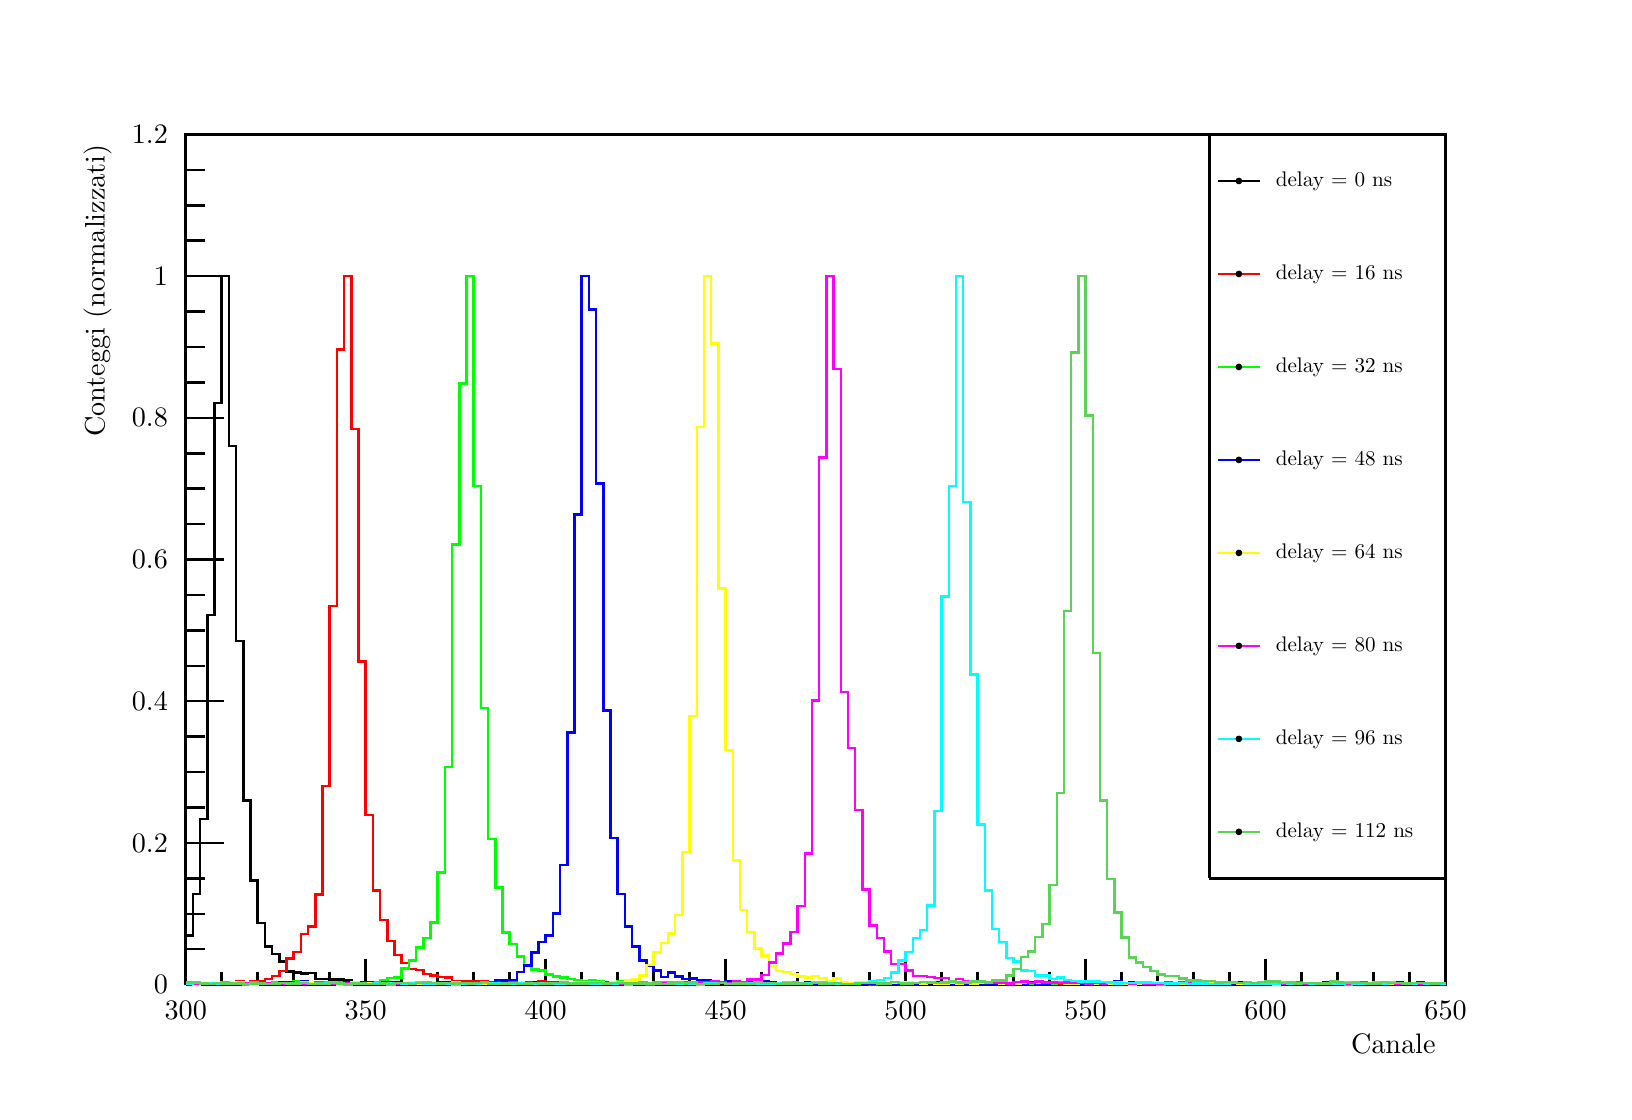
\begin{tikzpicture}
\pgfdeclareplotmark{cross} {
\pgfpathmoveto{\pgfpoint{-0.3\pgfplotmarksize}{\pgfplotmarksize}}
\pgfpathlineto{\pgfpoint{+0.3\pgfplotmarksize}{\pgfplotmarksize}}
\pgfpathlineto{\pgfpoint{+0.3\pgfplotmarksize}{0.3\pgfplotmarksize}}
\pgfpathlineto{\pgfpoint{+1\pgfplotmarksize}{0.3\pgfplotmarksize}}
\pgfpathlineto{\pgfpoint{+1\pgfplotmarksize}{-0.3\pgfplotmarksize}}
\pgfpathlineto{\pgfpoint{+0.3\pgfplotmarksize}{-0.3\pgfplotmarksize}}
\pgfpathlineto{\pgfpoint{+0.3\pgfplotmarksize}{-1.\pgfplotmarksize}}
\pgfpathlineto{\pgfpoint{-0.3\pgfplotmarksize}{-1.\pgfplotmarksize}}
\pgfpathlineto{\pgfpoint{-0.3\pgfplotmarksize}{-0.3\pgfplotmarksize}}
\pgfpathlineto{\pgfpoint{-1.\pgfplotmarksize}{-0.3\pgfplotmarksize}}
\pgfpathlineto{\pgfpoint{-1.\pgfplotmarksize}{0.3\pgfplotmarksize}}
\pgfpathlineto{\pgfpoint{-0.3\pgfplotmarksize}{0.3\pgfplotmarksize}}
\pgfpathclose
\pgfusepathqstroke
}
\pgfdeclareplotmark{cross*} {
\pgfpathmoveto{\pgfpoint{-0.3\pgfplotmarksize}{\pgfplotmarksize}}
\pgfpathlineto{\pgfpoint{+0.3\pgfplotmarksize}{\pgfplotmarksize}}
\pgfpathlineto{\pgfpoint{+0.3\pgfplotmarksize}{0.3\pgfplotmarksize}}
\pgfpathlineto{\pgfpoint{+1\pgfplotmarksize}{0.3\pgfplotmarksize}}
\pgfpathlineto{\pgfpoint{+1\pgfplotmarksize}{-0.3\pgfplotmarksize}}
\pgfpathlineto{\pgfpoint{+0.3\pgfplotmarksize}{-0.3\pgfplotmarksize}}
\pgfpathlineto{\pgfpoint{+0.3\pgfplotmarksize}{-1.\pgfplotmarksize}}
\pgfpathlineto{\pgfpoint{-0.3\pgfplotmarksize}{-1.\pgfplotmarksize}}
\pgfpathlineto{\pgfpoint{-0.3\pgfplotmarksize}{-0.3\pgfplotmarksize}}
\pgfpathlineto{\pgfpoint{-1.\pgfplotmarksize}{-0.3\pgfplotmarksize}}
\pgfpathlineto{\pgfpoint{-1.\pgfplotmarksize}{0.3\pgfplotmarksize}}
\pgfpathlineto{\pgfpoint{-0.3\pgfplotmarksize}{0.3\pgfplotmarksize}}
\pgfpathclose
\pgfusepathqfillstroke
}
\pgfdeclareplotmark{newstar} {
\pgfpathmoveto{\pgfqpoint{0pt}{\pgfplotmarksize}}
\pgfpathlineto{\pgfqpointpolar{44}{0.5\pgfplotmarksize}}
\pgfpathlineto{\pgfqpointpolar{18}{\pgfplotmarksize}}
\pgfpathlineto{\pgfqpointpolar{-20}{0.5\pgfplotmarksize}}
\pgfpathlineto{\pgfqpointpolar{-54}{\pgfplotmarksize}}
\pgfpathlineto{\pgfqpointpolar{-90}{0.5\pgfplotmarksize}}
\pgfpathlineto{\pgfqpointpolar{234}{\pgfplotmarksize}}
\pgfpathlineto{\pgfqpointpolar{198}{0.5\pgfplotmarksize}}
\pgfpathlineto{\pgfqpointpolar{162}{\pgfplotmarksize}}
\pgfpathlineto{\pgfqpointpolar{134}{0.5\pgfplotmarksize}}
\pgfpathclose
\pgfusepathqstroke
}
\pgfdeclareplotmark{newstar*} {
\pgfpathmoveto{\pgfqpoint{0pt}{\pgfplotmarksize}}
\pgfpathlineto{\pgfqpointpolar{44}{0.5\pgfplotmarksize}}
\pgfpathlineto{\pgfqpointpolar{18}{\pgfplotmarksize}}
\pgfpathlineto{\pgfqpointpolar{-20}{0.5\pgfplotmarksize}}
\pgfpathlineto{\pgfqpointpolar{-54}{\pgfplotmarksize}}
\pgfpathlineto{\pgfqpointpolar{-90}{0.5\pgfplotmarksize}}
\pgfpathlineto{\pgfqpointpolar{234}{\pgfplotmarksize}}
\pgfpathlineto{\pgfqpointpolar{198}{0.5\pgfplotmarksize}}
\pgfpathlineto{\pgfqpointpolar{162}{\pgfplotmarksize}}
\pgfpathlineto{\pgfqpointpolar{134}{0.5\pgfplotmarksize}}
\pgfpathclose
\pgfusepathqfillstroke
}
\definecolor{c}{rgb}{1,1,1};
\draw [color=c, fill=c] (0,0) rectangle (20,13.4957);
\draw [color=c, fill=c] (2,1.34957) rectangle (18,12.1461);
\definecolor{c}{rgb}{0,0,0};
\draw [c,line width=0.9] (2,1.34957) -- (2,12.1461) -- (18,12.1461) -- (18,1.34957) -- (2,1.34957);
\definecolor{c}{rgb}{1,1,1};
\draw [color=c, fill=c] (2,1.34957) rectangle (18,12.1461);
\definecolor{c}{rgb}{0,0,0};
\draw [c,line width=0.9] (2,1.34957) -- (2,12.1461) -- (18,12.1461) -- (18,1.34957) -- (2,1.34957);
\draw [c,line width=0.9] (2,1.97502) -- (2.09143,1.97502) -- (2.09143,2.50101) -- (2.18286,2.50101) -- (2.18286,3.45575) -- (2.27429,3.45575) -- (2.27429,6.04373) -- (2.36571,6.04373) -- (2.36571,8.73336) -- (2.45714,8.73336) -- (2.45714,10.3467) --
 (2.54857,10.3467) -- (2.54857,8.18969) -- (2.64,8.18969) -- (2.64,5.71664) -- (2.73143,5.71664) -- (2.73143,3.6856) -- (2.82286,3.6856) -- (2.82286,2.67118) -- (2.91429,2.67118) -- (2.91429,2.13414) -- (3.00571,2.13414) -- (3.00571,1.83578) --
 (3.09714,1.83578) -- (3.09714,1.73854) -- (3.18857,1.73854) -- (3.18857,1.64351) -- (3.28,1.64351) -- (3.28,1.51532) -- (3.37143,1.51532) -- (3.37143,1.50206) -- (3.46286,1.50206) -- (3.46286,1.49101) -- (3.55429,1.49101) -- (3.55429,1.49764) --
 (3.64571,1.49764) -- (3.64571,1.4225) -- (3.73714,1.4225) -- (3.73714,1.42029) -- (3.82857,1.42029) -- (3.82857,1.41366) -- (3.92,1.41366) -- (3.92,1.41587) -- (4.01143,1.41587) -- (4.01143,1.40482) -- (4.10286,1.40482) -- (4.10286,1.38493) --
 (4.19429,1.38493) -- (4.19429,1.38493) -- (4.28571,1.38493) -- (4.28571,1.37167) -- (4.37714,1.37167) -- (4.37714,1.38272) -- (4.46857,1.38272) -- (4.46857,1.37609) -- (4.56,1.37609) -- (4.56,1.38493) -- (4.65143,1.38493) -- (4.65143,1.37609) --
 (4.74286,1.37609) -- (4.74286,1.36946) -- (4.83429,1.36946) -- (4.83429,1.37388) -- (4.92571,1.37388) -- (4.92571,1.36504) -- (5.01714,1.36504) -- (5.01714,1.37167) -- (5.10857,1.37167) -- (5.10857,1.36946) -- (5.2,1.36946) -- (5.2,1.37609) --
 (5.29143,1.37609) -- (5.29143,1.36946) -- (5.38286,1.36946) -- (5.38286,1.37609) -- (5.47429,1.37609) -- (5.47429,1.37167) -- (5.56571,1.37167) -- (5.56571,1.36946) -- (5.65714,1.36946) -- (5.65714,1.35399) -- (5.74857,1.35399) -- (5.74857,1.36946)
 -- (5.84,1.36946) -- (5.84,1.36062) -- (5.93143,1.36062) -- (5.93143,1.36504) -- (6.02286,1.36504) -- (6.02286,1.36946) -- (6.11429,1.36946) -- (6.11429,1.36062) -- (6.20571,1.36062) -- (6.20571,1.36504) -- (6.29714,1.36504) -- (6.29714,1.36725) --
 (6.38857,1.36725) -- (6.38857,1.37388) -- (6.48,1.37388) -- (6.48,1.36946) -- (6.57143,1.36946) -- (6.57143,1.36283) -- (6.66286,1.36283) -- (6.66286,1.36946) -- (6.75429,1.36946) -- (6.75429,1.3783) -- (6.84571,1.3783) -- (6.84571,1.36946) --
 (6.93714,1.36946) -- (6.93714,1.37167) -- (7.02857,1.37167) -- (7.02857,1.37609) -- (7.12,1.37609) -- (7.12,1.3783) -- (7.21143,1.3783) -- (7.21143,1.36283) -- (7.30286,1.36283) -- (7.30286,1.37167) -- (7.39429,1.37167) -- (7.39429,1.37167) --
 (7.48571,1.37167) -- (7.48571,1.37388) -- (7.57714,1.37388) -- (7.57714,1.35399) -- (7.66857,1.35399) -- (7.66857,1.37167) -- (7.76,1.37167) -- (7.76,1.36725) -- (7.85143,1.36725) -- (7.85143,1.36946) -- (7.94286,1.36946) -- (7.94286,1.37609) --
 (8.03429,1.37609) -- (8.03429,1.36504) -- (8.12571,1.36504) -- (8.12571,1.3562) -- (8.21714,1.3562) -- (8.21714,1.35841) -- (8.30857,1.35841) -- (8.30857,1.36504) -- (8.4,1.36504) -- (8.4,1.36283) -- (8.49143,1.36283) -- (8.49143,1.36504) --
 (8.58286,1.36504) -- (8.58286,1.3783) -- (8.67429,1.3783) -- (8.67429,1.36504) -- (8.76571,1.36504) -- (8.76571,1.36725) -- (8.85714,1.36725) -- (8.85714,1.36062) -- (8.94857,1.36062) -- (8.94857,1.36062) -- (9.04,1.36062) -- (9.04,1.37167) --
 (9.13143,1.37167) -- (9.13143,1.36946) -- (9.22286,1.36946) -- (9.22286,1.36725) -- (9.31429,1.36725) -- (9.31429,1.36725) -- (9.40571,1.36725) -- (9.40571,1.37167) -- (9.49714,1.37167) -- (9.49714,1.36725) -- (9.58857,1.36725) -- (9.58857,1.36504)
 -- (9.68,1.36504) -- (9.68,1.36283) -- (9.77143,1.36283) -- (9.77143,1.36283) -- (9.86286,1.36283) -- (9.86286,1.36062) -- (9.95429,1.36062) -- (9.95429,1.36062) -- (10.0457,1.36062) -- (10.0457,1.36283) -- (10.1371,1.36283) -- (10.1371,1.37609) --
 (10.2286,1.37609) -- (10.2286,1.36725) -- (10.32,1.36725) -- (10.32,1.35841) -- (10.4114,1.35841) -- (10.4114,1.36283) -- (10.5029,1.36283) -- (10.5029,1.36062) -- (10.5943,1.36062) -- (10.5943,1.36504) -- (10.6857,1.36504) -- (10.6857,1.36504) --
 (10.7771,1.36504) -- (10.7771,1.36946) -- (10.8686,1.36946) -- (10.8686,1.37167) -- (10.96,1.37167) -- (10.96,1.36946) -- (11.0514,1.36946) -- (11.0514,1.35399) -- (11.1429,1.35399) -- (11.1429,1.36283) -- (11.2343,1.36283) -- (11.2343,1.35841) --
 (11.3257,1.35841) -- (11.3257,1.36725) -- (11.4171,1.36725) -- (11.4171,1.36504) -- (11.5086,1.36504) -- (11.5086,1.37167) -- (11.6,1.37167) -- (11.6,1.36062) -- (11.6914,1.36062) -- (11.6914,1.35399) -- (11.7829,1.35399) -- (11.7829,1.36504) --
 (11.8743,1.36504) -- (11.8743,1.3562) -- (11.9657,1.3562) -- (11.9657,1.35841) -- (12.0571,1.35841) -- (12.0571,1.3783) -- (12.1486,1.3783) -- (12.1486,1.36062) -- (12.24,1.36062) -- (12.24,1.36283) -- (12.3314,1.36283) -- (12.3314,1.36725) --
 (12.4229,1.36725) -- (12.4229,1.36725) -- (12.5143,1.36725) -- (12.5143,1.37609) -- (12.6057,1.37609) -- (12.6057,1.36504) -- (12.6971,1.36504) -- (12.6971,1.36725) -- (12.7886,1.36725) -- (12.7886,1.36504) -- (12.88,1.36504) -- (12.88,1.36283) --
 (12.9714,1.36283) -- (12.9714,1.36725) -- (13.0629,1.36725) -- (13.0629,1.3562) -- (13.1543,1.3562) -- (13.1543,1.36946) -- (13.2457,1.36946) -- (13.2457,1.36283) -- (13.3371,1.36283) -- (13.3371,1.36062) -- (13.4286,1.36062) -- (13.4286,1.36283) --
 (13.52,1.36283) -- (13.52,1.35178) -- (13.6114,1.35178) -- (13.6114,1.36946) -- (13.7029,1.36946) -- (13.7029,1.36062) -- (13.7943,1.36062) -- (13.7943,1.36946) -- (13.8857,1.36946) -- (13.8857,1.36283) -- (13.9771,1.36283) -- (13.9771,1.37609) --
 (14.0686,1.37609) -- (14.0686,1.36504) -- (14.16,1.36504) -- (14.16,1.37167) -- (14.2514,1.37167) -- (14.2514,1.37167) -- (14.3429,1.37167) -- (14.3429,1.36062) -- (14.4343,1.36062) -- (14.4343,1.3562) -- (14.5257,1.3562) -- (14.5257,1.36283) --
 (14.6171,1.36283) -- (14.6171,1.35841) -- (14.7086,1.35841) -- (14.7086,1.36946) -- (14.8,1.36946) -- (14.8,1.36504) -- (14.8914,1.36504) -- (14.8914,1.37609) -- (14.9829,1.37609) -- (14.9829,1.35841) -- (15.0743,1.35841) -- (15.0743,1.3562) --
 (15.1657,1.3562) -- (15.1657,1.36946) -- (15.2571,1.36946) -- (15.2571,1.36283) -- (15.3486,1.36283) -- (15.3486,1.37609) -- (15.44,1.37609) -- (15.44,1.36504) -- (15.5314,1.36504) -- (15.5314,1.36283) -- (15.6229,1.36283) -- (15.6229,1.36283) --
 (15.7143,1.36283) -- (15.7143,1.36946) -- (15.8057,1.36946) -- (15.8057,1.36283) -- (15.8971,1.36283) -- (15.8971,1.35841) -- (15.9886,1.35841) -- (15.9886,1.36725) -- (16.08,1.36725) -- (16.08,1.36283) -- (16.1714,1.36283) -- (16.1714,1.36725) --
 (16.2629,1.36725) -- (16.2629,1.35841) -- (16.3543,1.35841) -- (16.3543,1.36725) -- (16.4457,1.36725) -- (16.4457,1.37388) -- (16.5371,1.37388) -- (16.5371,1.36725) -- (16.6286,1.36725) -- (16.6286,1.37388) -- (16.72,1.37388) -- (16.72,1.37609) --
 (16.8114,1.37609) -- (16.8114,1.37388) -- (16.9029,1.37388) -- (16.9029,1.36283) -- (16.9943,1.36283) -- (16.9943,1.37167) -- (17.0857,1.37167) -- (17.0857,1.36062) -- (17.1771,1.36062) -- (17.1771,1.36283) -- (17.2686,1.36283) -- (17.2686,1.37388)
 -- (17.36,1.37388) -- (17.36,1.35841) -- (17.4514,1.35841) -- (17.4514,1.36283) -- (17.5429,1.36283) -- (17.5429,1.36946) -- (17.6343,1.36946) -- (17.6343,1.36283) -- (17.7257,1.36283) -- (17.7257,1.36946) -- (17.8171,1.36946) -- (17.8171,1.36946)
 -- (17.9086,1.36946) -- (17.9086,1.36504) -- (18,1.36504);
\draw [c,line width=0.9] (2,1.34957) -- (18,1.34957);
\draw [anchor= east] (18,0.593811) node[scale=1.01821, color=c, rotate=0]{Canale};
\draw [c,line width=0.9] (2,1.67347) -- (2,1.34957);
\draw [c,line width=0.9] (2.45714,1.51152) -- (2.45714,1.34957);
\draw [c,line width=0.9] (2.91429,1.51152) -- (2.91429,1.34957);
\draw [c,line width=0.9] (3.37143,1.51152) -- (3.37143,1.34957);
\draw [c,line width=0.9] (3.82857,1.51152) -- (3.82857,1.34957);
\draw [c,line width=0.9] (4.28571,1.67347) -- (4.28571,1.34957);
\draw [c,line width=0.9] (4.74286,1.51152) -- (4.74286,1.34957);
\draw [c,line width=0.9] (5.2,1.51152) -- (5.2,1.34957);
\draw [c,line width=0.9] (5.65714,1.51152) -- (5.65714,1.34957);
\draw [c,line width=0.9] (6.11429,1.51152) -- (6.11429,1.34957);
\draw [c,line width=0.9] (6.57143,1.67347) -- (6.57143,1.34957);
\draw [c,line width=0.9] (7.02857,1.51152) -- (7.02857,1.34957);
\draw [c,line width=0.9] (7.48571,1.51152) -- (7.48571,1.34957);
\draw [c,line width=0.9] (7.94286,1.51152) -- (7.94286,1.34957);
\draw [c,line width=0.9] (8.4,1.51152) -- (8.4,1.34957);
\draw [c,line width=0.9] (8.85714,1.67347) -- (8.85714,1.34957);
\draw [c,line width=0.9] (9.31429,1.51152) -- (9.31429,1.34957);
\draw [c,line width=0.9] (9.77143,1.51152) -- (9.77143,1.34957);
\draw [c,line width=0.9] (10.2286,1.51152) -- (10.2286,1.34957);
\draw [c,line width=0.9] (10.6857,1.51152) -- (10.6857,1.34957);
\draw [c,line width=0.9] (11.1429,1.67347) -- (11.1429,1.34957);
\draw [c,line width=0.9] (11.6,1.51152) -- (11.6,1.34957);
\draw [c,line width=0.9] (12.0571,1.51152) -- (12.0571,1.34957);
\draw [c,line width=0.9] (12.5143,1.51152) -- (12.5143,1.34957);
\draw [c,line width=0.9] (12.9714,1.51152) -- (12.9714,1.34957);
\draw [c,line width=0.9] (13.4286,1.67347) -- (13.4286,1.34957);
\draw [c,line width=0.9] (13.8857,1.51152) -- (13.8857,1.34957);
\draw [c,line width=0.9] (14.3429,1.51152) -- (14.3429,1.34957);
\draw [c,line width=0.9] (14.8,1.51152) -- (14.8,1.34957);
\draw [c,line width=0.9] (15.2571,1.51152) -- (15.2571,1.34957);
\draw [c,line width=0.9] (15.7143,1.67347) -- (15.7143,1.34957);
\draw [c,line width=0.9] (16.1714,1.51152) -- (16.1714,1.34957);
\draw [c,line width=0.9] (16.6286,1.51152) -- (16.6286,1.34957);
\draw [c,line width=0.9] (17.0857,1.51152) -- (17.0857,1.34957);
\draw [c,line width=0.9] (17.5429,1.51152) -- (17.5429,1.34957);
\draw [c,line width=0.9] (18,1.67347) -- (18,1.34957);
\draw [anchor=base] (2,0.904212) node[scale=1.01821, color=c, rotate=0]{300};
\draw [anchor=base] (4.28571,0.904212) node[scale=1.01821, color=c, rotate=0]{350};
\draw [anchor=base] (6.57143,0.904212) node[scale=1.01821, color=c, rotate=0]{400};
\draw [anchor=base] (8.85714,0.904212) node[scale=1.01821, color=c, rotate=0]{450};
\draw [anchor=base] (11.1429,0.904212) node[scale=1.01821, color=c, rotate=0]{500};
\draw [anchor=base] (13.4286,0.904212) node[scale=1.01821, color=c, rotate=0]{550};
\draw [anchor=base] (15.7143,0.904212) node[scale=1.01821, color=c, rotate=0]{600};
\draw [anchor=base] (18,0.904212) node[scale=1.01821, color=c, rotate=0]{650};
\draw [c,line width=0.9] (2,1.34957) -- (2,12.1461);
\draw [anchor= east] (0.88,12.1461) node[scale=1.01821, color=c, rotate=90]{Conteggi (normalizzati)};
\draw [c,line width=0.9] (2.48,1.34957) -- (2,1.34957);
\draw [c,line width=0.9] (2.24,1.79943) -- (2,1.79943);
\draw [c,line width=0.9] (2.24,2.24928) -- (2,2.24928);
\draw [c,line width=0.9] (2.24,2.69914) -- (2,2.69914);
\draw [c,line width=0.9] (2.48,3.149) -- (2,3.149);
\draw [c,line width=0.9] (2.24,3.59885) -- (2,3.59885);
\draw [c,line width=0.9] (2.24,4.04871) -- (2,4.04871);
\draw [c,line width=0.9] (2.24,4.49857) -- (2,4.49857);
\draw [c,line width=0.9] (2.48,4.94842) -- (2,4.94842);
\draw [c,line width=0.9] (2.24,5.39828) -- (2,5.39828);
\draw [c,line width=0.9] (2.24,5.84814) -- (2,5.84814);
\draw [c,line width=0.9] (2.24,6.29799) -- (2,6.29799);
\draw [c,line width=0.9] (2.48,6.74785) -- (2,6.74785);
\draw [c,line width=0.9] (2.24,7.19771) -- (2,7.19771);
\draw [c,line width=0.9] (2.24,7.64756) -- (2,7.64756);
\draw [c,line width=0.9] (2.24,8.09742) -- (2,8.09742);
\draw [c,line width=0.9] (2.48,8.54728) -- (2,8.54728);
\draw [c,line width=0.9] (2.24,8.99713) -- (2,8.99713);
\draw [c,line width=0.9] (2.24,9.44699) -- (2,9.44699);
\draw [c,line width=0.9] (2.24,9.89685) -- (2,9.89685);
\draw [c,line width=0.9] (2.48,10.3467) -- (2,10.3467);
\draw [c,line width=0.9] (2.24,10.7966) -- (2,10.7966);
\draw [c,line width=0.9] (2.24,11.2464) -- (2,11.2464);
\draw [c,line width=0.9] (2.24,11.6963) -- (2,11.6963);
\draw [c,line width=0.9] (2.48,12.1461) -- (2,12.1461);
\draw [c,line width=0.9] (2.48,12.1461) -- (2,12.1461);
\draw [anchor= east] (1.9,1.34957) node[scale=1.01821, color=c, rotate=0]{0};
\draw [anchor= east] (1.9,3.149) node[scale=1.01821, color=c, rotate=0]{0.2};
\draw [anchor= east] (1.9,4.94842) node[scale=1.01821, color=c, rotate=0]{0.4};
\draw [anchor= east] (1.9,6.74785) node[scale=1.01821, color=c, rotate=0]{0.6};
\draw [anchor= east] (1.9,8.54728) node[scale=1.01821, color=c, rotate=0]{0.8};
\draw [anchor= east] (1.9,10.3467) node[scale=1.01821, color=c, rotate=0]{1};
\draw [anchor= east] (1.9,12.1461) node[scale=1.01821, color=c, rotate=0]{1.2};
\definecolor{c}{rgb}{1,0,0};
\draw [c,line width=0.9] (2,1.37694) -- (2.09143,1.37694) -- (2.09143,1.38151) -- (2.18286,1.38151) -- (2.18286,1.37238) -- (2.27429,1.37238) -- (2.27429,1.37238) -- (2.36571,1.37238) -- (2.36571,1.3701) -- (2.45714,1.3701) -- (2.45714,1.37694) --
 (2.54857,1.37694) -- (2.54857,1.36326) -- (2.64,1.36326) -- (2.64,1.39063) -- (2.73143,1.39063) -- (2.73143,1.36326) -- (2.82286,1.36326) -- (2.82286,1.39519) -- (2.91429,1.39519) -- (2.91429,1.39519) -- (3.00571,1.39519) -- (3.00571,1.42257) --
 (3.09714,1.42257) -- (3.09714,1.45907) -- (3.18857,1.45907) -- (3.18857,1.52066) -- (3.28,1.52066) -- (3.28,1.68035) -- (3.37143,1.68035) -- (3.37143,1.76475) -- (3.46286,1.76475) -- (3.46286,1.99287) -- (3.55429,1.99287) -- (3.55429,2.08869) --
 (3.64571,2.08869) -- (3.64571,2.49702) -- (3.73714,2.49702) -- (3.73714,3.87032) -- (3.82857,3.87032) -- (3.82857,6.1561) -- (3.92,6.1561) -- (3.92,9.41597) -- (4.01143,9.41597) -- (4.01143,10.3467) -- (4.10286,10.3467) -- (4.10286,8.4031) --
 (4.19429,8.4031) -- (4.19429,5.45349) -- (4.28571,5.45349) -- (4.28571,3.50304) -- (4.37714,3.50304) -- (4.37714,2.54265) -- (4.46857,2.54265) -- (4.46857,2.17081) -- (4.56,2.17081) -- (4.56,1.90163) -- (4.65143,1.90163) -- (4.65143,1.72597) --
 (4.74286,1.72597) -- (4.74286,1.62104) -- (4.83429,1.62104) -- (4.83429,1.54576) -- (4.92571,1.54576) -- (4.92571,1.53207) -- (5.01714,1.53207) -- (5.01714,1.48644) -- (5.10857,1.48644) -- (5.10857,1.46363) -- (5.2,1.46363) -- (5.2,1.4431) --
 (5.29143,1.4431) -- (5.29143,1.44082) -- (5.38286,1.44082) -- (5.38286,1.39748) -- (5.47429,1.39748) -- (5.47429,1.39291) -- (5.56571,1.39291) -- (5.56571,1.38835) -- (5.65714,1.38835) -- (5.65714,1.39748) -- (5.74857,1.39748) -- (5.74857,1.39291)
 -- (5.84,1.39291) -- (5.84,1.38151) -- (5.93143,1.38151) -- (5.93143,1.38835) -- (6.02286,1.38835) -- (6.02286,1.38607) -- (6.11429,1.38607) -- (6.11429,1.38151) -- (6.20571,1.38151) -- (6.20571,1.38151) -- (6.29714,1.38151) -- (6.29714,1.37466) --
 (6.38857,1.37466) -- (6.38857,1.3701) -- (6.48,1.3701) -- (6.48,1.38835) -- (6.57143,1.38835) -- (6.57143,1.37694) -- (6.66286,1.37694) -- (6.66286,1.37466) -- (6.75429,1.37466) -- (6.75429,1.36782) -- (6.84571,1.36782) -- (6.84571,1.3587) --
 (6.93714,1.3587) -- (6.93714,1.3701) -- (7.02857,1.3701) -- (7.02857,1.36098) -- (7.12,1.36098) -- (7.12,1.36326) -- (7.21143,1.36326) -- (7.21143,1.36782) -- (7.30286,1.36782) -- (7.30286,1.37694) -- (7.39429,1.37694) -- (7.39429,1.37238) --
 (7.48571,1.37238) -- (7.48571,1.35641) -- (7.57714,1.35641) -- (7.57714,1.37238) -- (7.66857,1.37238) -- (7.66857,1.37238) -- (7.76,1.37238) -- (7.76,1.36098) -- (7.85143,1.36098) -- (7.85143,1.37238) -- (7.94286,1.37238) -- (7.94286,1.36782) --
 (8.03429,1.36782) -- (8.03429,1.36554) -- (8.12571,1.36554) -- (8.12571,1.36098) -- (8.21714,1.36098) -- (8.21714,1.3701) -- (8.30857,1.3701) -- (8.30857,1.36326) -- (8.4,1.36326) -- (8.4,1.37238) -- (8.49143,1.37238) -- (8.49143,1.3701) --
 (8.58286,1.3701) -- (8.58286,1.36326) -- (8.67429,1.36326) -- (8.67429,1.36782) -- (8.76571,1.36782) -- (8.76571,1.36782) -- (8.85714,1.36782) -- (8.85714,1.36554) -- (8.94857,1.36554) -- (8.94857,1.36326) -- (9.04,1.36326) -- (9.04,1.3587) --
 (9.13143,1.3587) -- (9.13143,1.3701) -- (9.22286,1.3701) -- (9.22286,1.36782) -- (9.31429,1.36782) -- (9.31429,1.36782) -- (9.40571,1.36782) -- (9.40571,1.37466) -- (9.49714,1.37466) -- (9.49714,1.3587) -- (9.58857,1.3587) -- (9.58857,1.36782) --
 (9.68,1.36782) -- (9.68,1.37238) -- (9.77143,1.37238) -- (9.77143,1.36782) -- (9.86286,1.36782) -- (9.86286,1.36326) -- (9.95429,1.36326) -- (9.95429,1.37923) -- (10.0457,1.37923) -- (10.0457,1.36554) -- (10.1371,1.36554) -- (10.1371,1.36326) --
 (10.2286,1.36326) -- (10.2286,1.36326) -- (10.32,1.36326) -- (10.32,1.36098) -- (10.4114,1.36098) -- (10.4114,1.36326) -- (10.5029,1.36326) -- (10.5029,1.37466) -- (10.5943,1.37466) -- (10.5943,1.36782) -- (10.6857,1.36782) -- (10.6857,1.35413) --
 (10.7771,1.35413) -- (10.7771,1.36554) -- (10.8686,1.36554) -- (10.8686,1.37238) -- (10.96,1.37238) -- (10.96,1.36098) -- (11.0514,1.36098) -- (11.0514,1.36326) -- (11.1429,1.36326) -- (11.1429,1.36326) -- (11.2343,1.36326) -- (11.2343,1.36326) --
 (11.3257,1.36326) -- (11.3257,1.38151) -- (11.4171,1.38151) -- (11.4171,1.36782) -- (11.5086,1.36782) -- (11.5086,1.36782) -- (11.6,1.36782) -- (11.6,1.38151) -- (11.6914,1.38151) -- (11.6914,1.36098) -- (11.7829,1.36098) -- (11.7829,1.37238) --
 (11.8743,1.37238) -- (11.8743,1.36326) -- (11.9657,1.36326) -- (11.9657,1.36554) -- (12.0571,1.36554) -- (12.0571,1.36326) -- (12.1486,1.36326) -- (12.1486,1.36326) -- (12.24,1.36326) -- (12.24,1.36554) -- (12.3314,1.36554) -- (12.3314,1.36554) --
 (12.4229,1.36554) -- (12.4229,1.36782) -- (12.5143,1.36782) -- (12.5143,1.3587) -- (12.6057,1.3587) -- (12.6057,1.36554) -- (12.6971,1.36554) -- (12.6971,1.36098) -- (12.7886,1.36098) -- (12.7886,1.37923) -- (12.88,1.37923) -- (12.88,1.3701) --
 (12.9714,1.3701) -- (12.9714,1.37466) -- (13.0629,1.37466) -- (13.0629,1.36098) -- (13.1543,1.36098) -- (13.1543,1.36098) -- (13.2457,1.36098) -- (13.2457,1.3701) -- (13.3371,1.3701) -- (13.3371,1.3701) -- (13.4286,1.3701) -- (13.4286,1.37694) --
 (13.52,1.37694) -- (13.52,1.36098) -- (13.6114,1.36098) -- (13.6114,1.36326) -- (13.7029,1.36326) -- (13.7029,1.37238) -- (13.7943,1.37238) -- (13.7943,1.37923) -- (13.8857,1.37923) -- (13.8857,1.36326) -- (13.9771,1.36326) -- (13.9771,1.35413) --
 (14.0686,1.35413) -- (14.0686,1.37238) -- (14.16,1.37238) -- (14.16,1.36554) -- (14.2514,1.36554) -- (14.2514,1.36782) -- (14.3429,1.36782) -- (14.3429,1.3587) -- (14.4343,1.3587) -- (14.4343,1.3587) -- (14.5257,1.3587) -- (14.5257,1.36098) --
 (14.6171,1.36098) -- (14.6171,1.3701) -- (14.7086,1.3701) -- (14.7086,1.3701) -- (14.8,1.3701) -- (14.8,1.36326) -- (14.8914,1.36326) -- (14.8914,1.37238) -- (14.9829,1.37238) -- (14.9829,1.3701) -- (15.0743,1.3701) -- (15.0743,1.36326) --
 (15.1657,1.36326) -- (15.1657,1.36782) -- (15.2571,1.36782) -- (15.2571,1.36326) -- (15.3486,1.36326) -- (15.3486,1.3587) -- (15.44,1.3587) -- (15.44,1.36782) -- (15.5314,1.36782) -- (15.5314,1.36554) -- (15.6229,1.36554) -- (15.6229,1.36098) --
 (15.7143,1.36098) -- (15.7143,1.36326) -- (15.8057,1.36326) -- (15.8057,1.36782) -- (15.8971,1.36782) -- (15.8971,1.36782) -- (15.9886,1.36782) -- (15.9886,1.36554) -- (16.08,1.36554) -- (16.08,1.37466) -- (16.1714,1.37466) -- (16.1714,1.36098) --
 (16.2629,1.36098) -- (16.2629,1.36782) -- (16.3543,1.36782) -- (16.3543,1.35641) -- (16.4457,1.35641) -- (16.4457,1.36554) -- (16.5371,1.36554) -- (16.5371,1.3701) -- (16.6286,1.3701) -- (16.6286,1.36326) -- (16.72,1.36326) -- (16.72,1.37238) --
 (16.8114,1.37238) -- (16.8114,1.36326) -- (16.9029,1.36326) -- (16.9029,1.36782) -- (16.9943,1.36782) -- (16.9943,1.37238) -- (17.0857,1.37238) -- (17.0857,1.36554) -- (17.1771,1.36554) -- (17.1771,1.36782) -- (17.2686,1.36782) -- (17.2686,1.37694)
 -- (17.36,1.37694) -- (17.36,1.36098) -- (17.4514,1.36098) -- (17.4514,1.3587) -- (17.5429,1.3587) -- (17.5429,1.36782) -- (17.6343,1.36782) -- (17.6343,1.36782) -- (17.7257,1.36782) -- (17.7257,1.3587) -- (17.8171,1.3587) -- (17.8171,1.3587) --
 (17.9086,1.3587) -- (17.9086,1.35641) -- (18,1.35641);
\definecolor{c}{rgb}{0,1,0};
\draw [c,line width=0.9] (2,1.37848) -- (2.09143,1.37848) -- (2.09143,1.36514) -- (2.18286,1.36514) -- (2.18286,1.35847) -- (2.27429,1.35847) -- (2.27429,1.36069) -- (2.36571,1.36069) -- (2.36571,1.36514) -- (2.45714,1.36514) -- (2.45714,1.37848) --
 (2.54857,1.37848) -- (2.54857,1.36514) -- (2.64,1.36514) -- (2.64,1.36958) -- (2.73143,1.36958) -- (2.73143,1.35402) -- (2.82286,1.35402) -- (2.82286,1.37403) -- (2.91429,1.37403) -- (2.91429,1.36736) -- (3.00571,1.36736) -- (3.00571,1.35624) --
 (3.09714,1.35624) -- (3.09714,1.37625) -- (3.18857,1.37625) -- (3.18857,1.36958) -- (3.28,1.36958) -- (3.28,1.36736) -- (3.37143,1.36736) -- (3.37143,1.38737) -- (3.46286,1.38737) -- (3.46286,1.37848) -- (3.55429,1.37848) -- (3.55429,1.36514) --
 (3.64571,1.36514) -- (3.64571,1.37848) -- (3.73714,1.37848) -- (3.73714,1.37403) -- (3.82857,1.37403) -- (3.82857,1.36958) -- (3.92,1.36958) -- (3.92,1.3807) -- (4.01143,1.3807) -- (4.01143,1.38293) -- (4.10286,1.38293) -- (4.10286,1.36514) --
 (4.19429,1.36514) -- (4.19429,1.36069) -- (4.28571,1.36069) -- (4.28571,1.37625) -- (4.37714,1.37625) -- (4.37714,1.38293) -- (4.46857,1.38293) -- (4.46857,1.40961) -- (4.56,1.40961) -- (4.56,1.4363) -- (4.65143,1.4363) -- (4.65143,1.44074) --
 (4.74286,1.44074) -- (4.74286,1.55415) -- (4.83429,1.55415) -- (4.83429,1.65867) -- (4.92571,1.65867) -- (4.92571,1.821) -- (5.01714,1.821) -- (5.01714,1.9433) -- (5.10857,1.9433) -- (5.10857,2.14121) -- (5.2,2.14121) -- (5.2,2.77497) --
 (5.29143,2.77497) -- (5.29143,4.11364) -- (5.38286,4.11364) -- (5.38286,6.93776) -- (5.47429,6.93776) -- (5.47429,8.98135) -- (5.56571,8.98135) -- (5.56571,10.3467) -- (5.65714,10.3467) -- (5.65714,7.68048) -- (5.74857,7.68048) -- (5.74857,4.86081)
 -- (5.84,4.86081) -- (5.84,3.20192) -- (5.93143,3.20192) -- (5.93143,2.58151) -- (6.02286,2.58151) -- (6.02286,2.01446) -- (6.11429,2.01446) -- (6.11429,1.86769) -- (6.20571,1.86769) -- (6.20571,1.70759) -- (6.29714,1.70759) -- (6.29714,1.60085) --
 (6.38857,1.60085) -- (6.38857,1.53859) -- (6.48,1.53859) -- (6.48,1.52747) -- (6.57143,1.52747) -- (6.57143,1.48077) -- (6.66286,1.48077) -- (6.66286,1.45186) -- (6.75429,1.45186) -- (6.75429,1.44297) -- (6.84571,1.44297) -- (6.84571,1.42073) --
 (6.93714,1.42073) -- (6.93714,1.40516) -- (7.02857,1.40516) -- (7.02857,1.39849) -- (7.12,1.39849) -- (7.12,1.40072) -- (7.21143,1.40072) -- (7.21143,1.39627) -- (7.30286,1.39627) -- (7.30286,1.37181) -- (7.39429,1.37181) -- (7.39429,1.3807) --
 (7.48571,1.3807) -- (7.48571,1.38737) -- (7.57714,1.38737) -- (7.57714,1.3896) -- (7.66857,1.3896) -- (7.66857,1.36958) -- (7.76,1.36958) -- (7.76,1.38293) -- (7.85143,1.38293) -- (7.85143,1.37181) -- (7.94286,1.37181) -- (7.94286,1.37403) --
 (8.03429,1.37403) -- (8.03429,1.37403) -- (8.12571,1.37403) -- (8.12571,1.37848) -- (8.21714,1.37848) -- (8.21714,1.37625) -- (8.30857,1.37625) -- (8.30857,1.35847) -- (8.4,1.35847) -- (8.4,1.37403) -- (8.49143,1.37403) -- (8.49143,1.36514) --
 (8.58286,1.36514) -- (8.58286,1.36291) -- (8.67429,1.36291) -- (8.67429,1.36069) -- (8.76571,1.36069) -- (8.76571,1.37625) -- (8.85714,1.37625) -- (8.85714,1.37403) -- (8.94857,1.37403) -- (8.94857,1.36069) -- (9.04,1.36069) -- (9.04,1.36736) --
 (9.13143,1.36736) -- (9.13143,1.35847) -- (9.22286,1.35847) -- (9.22286,1.36736) -- (9.31429,1.36736) -- (9.31429,1.37403) -- (9.40571,1.37403) -- (9.40571,1.36069) -- (9.49714,1.36069) -- (9.49714,1.36291) -- (9.58857,1.36291) -- (9.58857,1.36736)
 -- (9.68,1.36736) -- (9.68,1.38293) -- (9.77143,1.38293) -- (9.77143,1.35847) -- (9.86286,1.35847) -- (9.86286,1.36291) -- (9.95429,1.36291) -- (9.95429,1.37403) -- (10.0457,1.37403) -- (10.0457,1.36069) -- (10.1371,1.36069) -- (10.1371,1.36736) --
 (10.2286,1.36736) -- (10.2286,1.35847) -- (10.32,1.35847) -- (10.32,1.36291) -- (10.4114,1.36291) -- (10.4114,1.36514) -- (10.5029,1.36514) -- (10.5029,1.35847) -- (10.5943,1.35847) -- (10.5943,1.37625) -- (10.6857,1.37625) -- (10.6857,1.36736) --
 (10.7771,1.36736) -- (10.7771,1.37403) -- (10.8686,1.37403) -- (10.8686,1.36736) -- (10.96,1.36736) -- (10.96,1.35624) -- (11.0514,1.35624) -- (11.0514,1.36291) -- (11.1429,1.36291) -- (11.1429,1.36958) -- (11.2343,1.36958) -- (11.2343,1.36291) --
 (11.3257,1.36291) -- (11.3257,1.35847) -- (11.4171,1.35847) -- (11.4171,1.37403) -- (11.5086,1.37403) -- (11.5086,1.36069) -- (11.6,1.36069) -- (11.6,1.36514) -- (11.6914,1.36514) -- (11.6914,1.37181) -- (11.7829,1.37181) -- (11.7829,1.37403) --
 (11.8743,1.37403) -- (11.8743,1.36291) -- (11.9657,1.36291) -- (11.9657,1.35624) -- (12.0571,1.35624) -- (12.0571,1.35847) -- (12.1486,1.35847) -- (12.1486,1.36514) -- (12.24,1.36514) -- (12.24,1.37181) -- (12.3314,1.37181) -- (12.3314,1.35847) --
 (12.4229,1.35847) -- (12.4229,1.36736) -- (12.5143,1.36736) -- (12.5143,1.36736) -- (12.6057,1.36736) -- (12.6057,1.37181) -- (12.6971,1.37181) -- (12.6971,1.36069) -- (12.7886,1.36069) -- (12.7886,1.36291) -- (12.88,1.36291) -- (12.88,1.36736) --
 (12.9714,1.36736) -- (12.9714,1.35624) -- (13.0629,1.35624) -- (13.0629,1.38293) -- (13.1543,1.38293) -- (13.1543,1.36291) -- (13.2457,1.36291) -- (13.2457,1.36069) -- (13.3371,1.36069) -- (13.3371,1.35847) -- (13.4286,1.35847) -- (13.4286,1.35847)
 -- (13.52,1.35847) -- (13.52,1.36958) -- (13.6114,1.36958) -- (13.6114,1.36958) -- (13.7029,1.36958) -- (13.7029,1.36069) -- (13.7943,1.36069) -- (13.7943,1.37181) -- (13.8857,1.37181) -- (13.8857,1.35847) -- (13.9771,1.35847) -- (13.9771,1.36514)
 -- (14.0686,1.36514) -- (14.0686,1.36291) -- (14.16,1.36291) -- (14.16,1.36069) -- (14.2514,1.36069) -- (14.2514,1.35624) -- (14.3429,1.35624) -- (14.3429,1.35179) -- (14.4343,1.35179) -- (14.4343,1.36069) -- (14.5257,1.36069) -- (14.5257,1.36069)
 -- (14.6171,1.36069) -- (14.6171,1.36291) -- (14.7086,1.36291) -- (14.7086,1.36958) -- (14.8,1.36958) -- (14.8,1.35624) -- (14.8914,1.35624) -- (14.8914,1.36736) -- (14.9829,1.36736) -- (14.9829,1.36736) -- (15.0743,1.36736) -- (15.0743,1.36958) --
 (15.1657,1.36958) -- (15.1657,1.36736) -- (15.2571,1.36736) -- (15.2571,1.37403) -- (15.3486,1.37403) -- (15.3486,1.36736) -- (15.44,1.36736) -- (15.44,1.36069) -- (15.5314,1.36069) -- (15.5314,1.36069) -- (15.6229,1.36069) -- (15.6229,1.36069) --
 (15.7143,1.36069) -- (15.7143,1.36514) -- (15.8057,1.36514) -- (15.8057,1.36736) -- (15.8971,1.36736) -- (15.8971,1.37181) -- (15.9886,1.37181) -- (15.9886,1.36736) -- (16.08,1.36736) -- (16.08,1.35624) -- (16.1714,1.35624) -- (16.1714,1.36291) --
 (16.2629,1.36291) -- (16.2629,1.36069) -- (16.3543,1.36069) -- (16.3543,1.36514) -- (16.4457,1.36514) -- (16.4457,1.36291) -- (16.5371,1.36291) -- (16.5371,1.36958) -- (16.6286,1.36958) -- (16.6286,1.37403) -- (16.72,1.37403) -- (16.72,1.35402) --
 (16.8114,1.35402) -- (16.8114,1.36291) -- (16.9029,1.36291) -- (16.9029,1.36514) -- (16.9943,1.36514) -- (16.9943,1.36291) -- (17.0857,1.36291) -- (17.0857,1.37181) -- (17.1771,1.37181) -- (17.1771,1.35624) -- (17.2686,1.35624) -- (17.2686,1.36736)
 -- (17.36,1.36736) -- (17.36,1.35847) -- (17.4514,1.35847) -- (17.4514,1.36291) -- (17.5429,1.36291) -- (17.5429,1.36736) -- (17.6343,1.36736) -- (17.6343,1.36291) -- (17.7257,1.36291) -- (17.7257,1.35624) -- (17.8171,1.35624) -- (17.8171,1.36291)
 -- (17.9086,1.36291) -- (17.9086,1.36291) -- (18,1.36291);
\definecolor{c}{rgb}{0,0,1};
\draw [c,line width=0.9] (2,1.36857) -- (2.09143,1.36857) -- (2.09143,1.37569) -- (2.18286,1.37569) -- (2.18286,1.35907) -- (2.27429,1.35907) -- (2.27429,1.36619) -- (2.36571,1.36619) -- (2.36571,1.36619) -- (2.45714,1.36619) -- (2.45714,1.36144) --
 (2.54857,1.36144) -- (2.54857,1.35432) -- (2.64,1.35432) -- (2.64,1.35432) -- (2.73143,1.35432) -- (2.73143,1.36382) -- (2.82286,1.36382) -- (2.82286,1.36382) -- (2.91429,1.36382) -- (2.91429,1.35907) -- (3.00571,1.35907) -- (3.00571,1.36619) --
 (3.09714,1.36619) -- (3.09714,1.36382) -- (3.18857,1.36382) -- (3.18857,1.37806) -- (3.28,1.37806) -- (3.28,1.37569) -- (3.37143,1.37569) -- (3.37143,1.37094) -- (3.46286,1.37094) -- (3.46286,1.38756) -- (3.55429,1.38756) -- (3.55429,1.37094) --
 (3.64571,1.37094) -- (3.64571,1.36144) -- (3.73714,1.36144) -- (3.73714,1.36382) -- (3.82857,1.36382) -- (3.82857,1.36619) -- (3.92,1.36619) -- (3.92,1.36619) -- (4.01143,1.36619) -- (4.01143,1.37332) -- (4.10286,1.37332) -- (4.10286,1.36144) --
 (4.19429,1.36144) -- (4.19429,1.36144) -- (4.28571,1.36144) -- (4.28571,1.37332) -- (4.37714,1.37332) -- (4.37714,1.36382) -- (4.46857,1.36382) -- (4.46857,1.36857) -- (4.56,1.36857) -- (4.56,1.37094) -- (4.65143,1.37094) -- (4.65143,1.38281) --
 (4.74286,1.38281) -- (4.74286,1.36144) -- (4.83429,1.36144) -- (4.83429,1.37332) -- (4.92571,1.37332) -- (4.92571,1.36619) -- (5.01714,1.36619) -- (5.01714,1.38044) -- (5.10857,1.38044) -- (5.10857,1.36857) -- (5.2,1.36857) -- (5.2,1.37332) --
 (5.29143,1.37332) -- (5.29143,1.37332) -- (5.38286,1.37332) -- (5.38286,1.37569) -- (5.47429,1.37569) -- (5.47429,1.35907) -- (5.56571,1.35907) -- (5.56571,1.35907) -- (5.65714,1.35907) -- (5.65714,1.36857) -- (5.74857,1.36857) -- (5.74857,1.38044)
 -- (5.84,1.38044) -- (5.84,1.36857) -- (5.93143,1.36857) -- (5.93143,1.40893) -- (6.02286,1.40893) -- (6.02286,1.40181) -- (6.11429,1.40181) -- (6.11429,1.40181) -- (6.20571,1.40181) -- (6.20571,1.50866) -- (6.29714,1.50866) -- (6.29714,1.59177) --
 (6.38857,1.59177) -- (6.38857,1.75799) -- (6.48,1.75799) -- (6.48,1.89334) -- (6.57143,1.89334) -- (6.57143,1.9717) -- (6.66286,1.9717) -- (6.66286,2.2519) -- (6.75429,2.2519) -- (6.75429,2.86928) -- (6.84571,2.86928) -- (6.84571,4.55283) --
 (6.93714,4.55283) -- (6.93714,7.31917) -- (7.02857,7.31917) -- (7.02857,10.3467) -- (7.12,10.3467) -- (7.12,9.92641) -- (7.21143,9.92641) -- (7.21143,7.71096) -- (7.30286,7.71096) -- (7.30286,4.83065) -- (7.39429,4.83065) -- (7.39429,3.21121) --
 (7.48571,3.21121) -- (7.48571,2.50122) -- (7.57714,2.50122) -- (7.57714,2.08805) -- (7.66857,2.08805) -- (7.66857,1.8316) -- (7.76,1.8316) -- (7.76,1.65826) -- (7.85143,1.65826) -- (7.85143,1.58702) -- (7.94286,1.58702) -- (7.94286,1.53004) --
 (8.03429,1.53004) -- (8.03429,1.4493) -- (8.12571,1.4493) -- (8.12571,1.50392) -- (8.21714,1.50392) -- (8.21714,1.45168) -- (8.30857,1.45168) -- (8.30857,1.42081) -- (8.4,1.42081) -- (8.4,1.42556) -- (8.49143,1.42556) -- (8.49143,1.41131) --
 (8.58286,1.41131) -- (8.58286,1.40418) -- (8.67429,1.40418) -- (8.67429,1.38994) -- (8.76571,1.38994) -- (8.76571,1.38044) -- (8.85714,1.38044) -- (8.85714,1.39706) -- (8.94857,1.39706) -- (8.94857,1.36619) -- (9.04,1.36619) -- (9.04,1.37569) --
 (9.13143,1.37569) -- (9.13143,1.37806) -- (9.22286,1.37806) -- (9.22286,1.40418) -- (9.31429,1.40418) -- (9.31429,1.38994) -- (9.40571,1.38994) -- (9.40571,1.37806) -- (9.49714,1.37806) -- (9.49714,1.37094) -- (9.58857,1.37094) -- (9.58857,1.37806)
 -- (9.68,1.37806) -- (9.68,1.36144) -- (9.77143,1.36144) -- (9.77143,1.35907) -- (9.86286,1.35907) -- (9.86286,1.38044) -- (9.95429,1.38044) -- (9.95429,1.36144) -- (10.0457,1.36144) -- (10.0457,1.37094) -- (10.1371,1.37094) -- (10.1371,1.37332) --
 (10.2286,1.37332) -- (10.2286,1.36144) -- (10.32,1.36144) -- (10.32,1.36619) -- (10.4114,1.36619) -- (10.4114,1.36144) -- (10.5029,1.36144) -- (10.5029,1.37094) -- (10.5943,1.37094) -- (10.5943,1.36382) -- (10.6857,1.36382) -- (10.6857,1.35669) --
 (10.7771,1.35669) -- (10.7771,1.36619) -- (10.8686,1.36619) -- (10.8686,1.36382) -- (10.96,1.36382) -- (10.96,1.36382) -- (11.0514,1.36382) -- (11.0514,1.37806) -- (11.1429,1.37806) -- (11.1429,1.36382) -- (11.2343,1.36382) -- (11.2343,1.35907) --
 (11.3257,1.35907) -- (11.3257,1.36382) -- (11.4171,1.36382) -- (11.4171,1.36857) -- (11.5086,1.36857) -- (11.5086,1.37806) -- (11.6,1.37806) -- (11.6,1.35669) -- (11.6914,1.35669) -- (11.6914,1.35669) -- (11.7829,1.35669) -- (11.7829,1.36382) --
 (11.8743,1.36382) -- (11.8743,1.36619) -- (11.9657,1.36619) -- (11.9657,1.36382) -- (12.0571,1.36382) -- (12.0571,1.36144) -- (12.1486,1.36144) -- (12.1486,1.36144) -- (12.24,1.36144) -- (12.24,1.36619) -- (12.3314,1.36619) -- (12.3314,1.36619) --
 (12.4229,1.36619) -- (12.4229,1.36382) -- (12.5143,1.36382) -- (12.5143,1.37332) -- (12.6057,1.37332) -- (12.6057,1.36382) -- (12.6971,1.36382) -- (12.6971,1.38044) -- (12.7886,1.38044) -- (12.7886,1.35907) -- (12.88,1.35907) -- (12.88,1.35669) --
 (12.9714,1.35669) -- (12.9714,1.36857) -- (13.0629,1.36857) -- (13.0629,1.37094) -- (13.1543,1.37094) -- (13.1543,1.35907) -- (13.2457,1.35907) -- (13.2457,1.37094) -- (13.3371,1.37094) -- (13.3371,1.36382) -- (13.4286,1.36382) -- (13.4286,1.36382)
 -- (13.52,1.36382) -- (13.52,1.36857) -- (13.6114,1.36857) -- (13.6114,1.37094) -- (13.7029,1.37094) -- (13.7029,1.36619) -- (13.7943,1.36619) -- (13.7943,1.38994) -- (13.8857,1.38994) -- (13.8857,1.36857) -- (13.9771,1.36857) -- (13.9771,1.38044)
 -- (14.0686,1.38044) -- (14.0686,1.36382) -- (14.16,1.36382) -- (14.16,1.34957) -- (14.2514,1.34957) -- (14.2514,1.37332) -- (14.3429,1.37332) -- (14.3429,1.37094) -- (14.4343,1.37094) -- (14.4343,1.36382) -- (14.5257,1.36382) -- (14.5257,1.36857)
 -- (14.6171,1.36857) -- (14.6171,1.36857) -- (14.7086,1.36857) -- (14.7086,1.36857) -- (14.8,1.36857) -- (14.8,1.37806) -- (14.8914,1.37806) -- (14.8914,1.37094) -- (14.9829,1.37094) -- (14.9829,1.35669) -- (15.0743,1.35669) -- (15.0743,1.35907) --
 (15.1657,1.35907) -- (15.1657,1.37569) -- (15.2571,1.37569) -- (15.2571,1.35907) -- (15.3486,1.35907) -- (15.3486,1.35669) -- (15.44,1.35669) -- (15.44,1.35432) -- (15.5314,1.35432) -- (15.5314,1.36857) -- (15.6229,1.36857) -- (15.6229,1.36619) --
 (15.7143,1.36619) -- (15.7143,1.36144) -- (15.8057,1.36144) -- (15.8057,1.36144) -- (15.8971,1.36144) -- (15.8971,1.37332) -- (15.9886,1.37332) -- (15.9886,1.36857) -- (16.08,1.36857) -- (16.08,1.36619) -- (16.1714,1.36619) -- (16.1714,1.35669) --
 (16.2629,1.35669) -- (16.2629,1.36857) -- (16.3543,1.36857) -- (16.3543,1.36857) -- (16.4457,1.36857) -- (16.4457,1.37332) -- (16.5371,1.37332) -- (16.5371,1.36619) -- (16.6286,1.36619) -- (16.6286,1.35907) -- (16.72,1.35907) -- (16.72,1.35669) --
 (16.8114,1.35669) -- (16.8114,1.37332) -- (16.9029,1.37332) -- (16.9029,1.35907) -- (16.9943,1.35907) -- (16.9943,1.35669) -- (17.0857,1.35669) -- (17.0857,1.36619) -- (17.1771,1.36619) -- (17.1771,1.35907) -- (17.2686,1.35907) -- (17.2686,1.37094)
 -- (17.36,1.37094) -- (17.36,1.37806) -- (17.4514,1.37806) -- (17.4514,1.36144) -- (17.5429,1.36144) -- (17.5429,1.36382) -- (17.6343,1.36382) -- (17.6343,1.37332) -- (17.7257,1.37332) -- (17.7257,1.36619) -- (17.8171,1.36619) -- (17.8171,1.36382)
 -- (17.9086,1.36382) -- (17.9086,1.36382) -- (18,1.36382);
\definecolor{c}{rgb}{1,1,0};
\draw [c,line width=0.9] (2,1.37005) -- (2.09143,1.37005) -- (2.09143,1.35185) -- (2.18286,1.35185) -- (2.18286,1.3655) -- (2.27429,1.3655) -- (2.27429,1.35867) -- (2.36571,1.35867) -- (2.36571,1.36777) -- (2.45714,1.36777) -- (2.45714,1.35867) --
 (2.54857,1.35867) -- (2.54857,1.36322) -- (2.64,1.36322) -- (2.64,1.3746) -- (2.73143,1.3746) -- (2.73143,1.36095) -- (2.82286,1.36095) -- (2.82286,1.35412) -- (2.91429,1.35412) -- (2.91429,1.36322) -- (3.00571,1.36322) -- (3.00571,1.36095) --
 (3.09714,1.36095) -- (3.09714,1.36322) -- (3.18857,1.36322) -- (3.18857,1.36777) -- (3.28,1.36777) -- (3.28,1.37232) -- (3.37143,1.37232) -- (3.37143,1.36095) -- (3.46286,1.36095) -- (3.46286,1.3746) -- (3.55429,1.3746) -- (3.55429,1.36322) --
 (3.64571,1.36322) -- (3.64571,1.35867) -- (3.73714,1.35867) -- (3.73714,1.36777) -- (3.82857,1.36777) -- (3.82857,1.36095) -- (3.92,1.36095) -- (3.92,1.35412) -- (4.01143,1.35412) -- (4.01143,1.36095) -- (4.10286,1.36095) -- (4.10286,1.3746) --
 (4.19429,1.3746) -- (4.19429,1.3655) -- (4.28571,1.3655) -- (4.28571,1.37005) -- (4.37714,1.37005) -- (4.37714,1.3655) -- (4.46857,1.3655) -- (4.46857,1.36322) -- (4.56,1.36322) -- (4.56,1.36777) -- (4.65143,1.36777) -- (4.65143,1.3564) --
 (4.74286,1.3564) -- (4.74286,1.36322) -- (4.83429,1.36322) -- (4.83429,1.3746) -- (4.92571,1.3746) -- (4.92571,1.36322) -- (5.01714,1.36322) -- (5.01714,1.36095) -- (5.10857,1.36095) -- (5.10857,1.37005) -- (5.2,1.37005) -- (5.2,1.37232) --
 (5.29143,1.37232) -- (5.29143,1.36322) -- (5.38286,1.36322) -- (5.38286,1.3746) -- (5.47429,1.3746) -- (5.47429,1.37005) -- (5.56571,1.37005) -- (5.56571,1.36777) -- (5.65714,1.36777) -- (5.65714,1.36777) -- (5.74857,1.36777) -- (5.74857,1.35867) --
 (5.84,1.35867) -- (5.84,1.36322) -- (5.93143,1.36322) -- (5.93143,1.36777) -- (6.02286,1.36777) -- (6.02286,1.3655) -- (6.11429,1.3655) -- (6.11429,1.37688) -- (6.20571,1.37688) -- (6.20571,1.37688) -- (6.29714,1.37688) -- (6.29714,1.36322) --
 (6.38857,1.36322) -- (6.38857,1.37232) -- (6.48,1.37232) -- (6.48,1.35867) -- (6.57143,1.35867) -- (6.57143,1.37005) -- (6.66286,1.37005) -- (6.66286,1.37232) -- (6.75429,1.37232) -- (6.75429,1.3837) -- (6.84571,1.3837) -- (6.84571,1.37005) --
 (6.93714,1.37005) -- (6.93714,1.36095) -- (7.02857,1.36095) -- (7.02857,1.3746) -- (7.12,1.3746) -- (7.12,1.37688) -- (7.21143,1.37688) -- (7.21143,1.3746) -- (7.30286,1.3746) -- (7.30286,1.37232) -- (7.39429,1.37232) -- (7.39429,1.38598) --
 (7.48571,1.38598) -- (7.48571,1.38143) -- (7.57714,1.38143) -- (7.57714,1.39963) -- (7.66857,1.39963) -- (7.66857,1.41328) -- (7.76,1.41328) -- (7.76,1.46562) -- (7.85143,1.46562) -- (7.85143,1.59759) -- (7.94286,1.59759) -- (7.94286,1.75915) --
 (8.03429,1.75915) -- (8.03429,1.87747) -- (8.12571,1.87747) -- (8.12571,1.99807) -- (8.21714,1.99807) -- (8.21714,2.23245) -- (8.30857,2.23245) -- (8.30857,3.03113) -- (8.4,3.03113) -- (8.4,4.76047) -- (8.49143,4.76047) -- (8.49143,8.43077) --
 (8.58286,8.43077) -- (8.58286,10.3467) -- (8.67429,10.3467) -- (8.67429,9.49341) -- (8.76571,9.49341) -- (8.76571,6.38287) -- (8.85714,6.38287) -- (8.85714,4.32814) -- (8.94857,4.32814) -- (8.94857,2.92418) -- (9.04,2.92418) -- (9.04,2.29843) --
 (9.13143,2.29843) -- (9.13143,2.01628) -- (9.22286,2.01628) -- (9.22286,1.80694) -- (9.31429,1.80694) -- (9.31429,1.72047) -- (9.40571,1.72047) -- (9.40571,1.58622) -- (9.49714,1.58622) -- (9.49714,1.52478) -- (9.58857,1.52478) -- (9.58857,1.50658)
 -- (9.68,1.50658) -- (9.68,1.48382) -- (9.77143,1.48382) -- (9.77143,1.45424) -- (9.86286,1.45424) -- (9.86286,1.43831) -- (9.95429,1.43831) -- (9.95429,1.46107) -- (10.0457,1.46107) -- (10.0457,1.43376) -- (10.1371,1.43376) -- (10.1371,1.39508) --
 (10.2286,1.39508) -- (10.2286,1.42694) -- (10.32,1.42694) -- (10.32,1.38598) -- (10.4114,1.38598) -- (10.4114,1.37005) -- (10.5029,1.37005) -- (10.5029,1.3837) -- (10.5943,1.3837) -- (10.5943,1.37915) -- (10.6857,1.37915) -- (10.6857,1.38143) --
 (10.7771,1.38143) -- (10.7771,1.3837) -- (10.8686,1.3837) -- (10.8686,1.37005) -- (10.96,1.37005) -- (10.96,1.37915) -- (11.0514,1.37915) -- (11.0514,1.37688) -- (11.1429,1.37688) -- (11.1429,1.37688) -- (11.2343,1.37688) -- (11.2343,1.37232) --
 (11.3257,1.37232) -- (11.3257,1.3655) -- (11.4171,1.3655) -- (11.4171,1.3746) -- (11.5086,1.3746) -- (11.5086,1.36095) -- (11.6,1.36095) -- (11.6,1.36322) -- (11.6914,1.36322) -- (11.6914,1.37232) -- (11.7829,1.37232) -- (11.7829,1.3655) --
 (11.8743,1.3655) -- (11.8743,1.37232) -- (11.9657,1.37232) -- (11.9657,1.3655) -- (12.0571,1.3655) -- (12.0571,1.36777) -- (12.1486,1.36777) -- (12.1486,1.37915) -- (12.24,1.37915) -- (12.24,1.37005) -- (12.3314,1.37005) -- (12.3314,1.36322) --
 (12.4229,1.36322) -- (12.4229,1.37688) -- (12.5143,1.37688) -- (12.5143,1.3655) -- (12.6057,1.3655) -- (12.6057,1.37915) -- (12.6971,1.37915) -- (12.6971,1.37005) -- (12.7886,1.37005) -- (12.7886,1.37005) -- (12.88,1.37005) -- (12.88,1.37005) --
 (12.9714,1.37005) -- (12.9714,1.37005) -- (13.0629,1.37005) -- (13.0629,1.37005) -- (13.1543,1.37005) -- (13.1543,1.35867) -- (13.2457,1.35867) -- (13.2457,1.3655) -- (13.3371,1.3655) -- (13.3371,1.37232) -- (13.4286,1.37232) -- (13.4286,1.36095) --
 (13.52,1.36095) -- (13.52,1.3655) -- (13.6114,1.3655) -- (13.6114,1.3746) -- (13.7029,1.3746) -- (13.7029,1.36322) -- (13.7943,1.36322) -- (13.7943,1.3746) -- (13.8857,1.3746) -- (13.8857,1.3655) -- (13.9771,1.3655) -- (13.9771,1.35412) --
 (14.0686,1.35412) -- (14.0686,1.36095) -- (14.16,1.36095) -- (14.16,1.36322) -- (14.2514,1.36322) -- (14.2514,1.38143) -- (14.3429,1.38143) -- (14.3429,1.37005) -- (14.4343,1.37005) -- (14.4343,1.37915) -- (14.5257,1.37915) -- (14.5257,1.37005) --
 (14.6171,1.37005) -- (14.6171,1.3564) -- (14.7086,1.3564) -- (14.7086,1.37232) -- (14.8,1.37232) -- (14.8,1.37688) -- (14.8914,1.37688) -- (14.8914,1.3655) -- (14.9829,1.3655) -- (14.9829,1.37005) -- (15.0743,1.37005) -- (15.0743,1.37005) --
 (15.1657,1.37005) -- (15.1657,1.37232) -- (15.2571,1.37232) -- (15.2571,1.3837) -- (15.3486,1.3837) -- (15.3486,1.36322) -- (15.44,1.36322) -- (15.44,1.36095) -- (15.5314,1.36095) -- (15.5314,1.36095) -- (15.6229,1.36095) -- (15.6229,1.37232) --
 (15.7143,1.37232) -- (15.7143,1.3746) -- (15.8057,1.3746) -- (15.8057,1.35185) -- (15.8971,1.35185) -- (15.8971,1.36777) -- (15.9886,1.36777) -- (15.9886,1.3655) -- (16.08,1.3655) -- (16.08,1.3655) -- (16.1714,1.3655) -- (16.1714,1.37005) --
 (16.2629,1.37005) -- (16.2629,1.37232) -- (16.3543,1.37232) -- (16.3543,1.3564) -- (16.4457,1.3564) -- (16.4457,1.3655) -- (16.5371,1.3655) -- (16.5371,1.36322) -- (16.6286,1.36322) -- (16.6286,1.36322) -- (16.72,1.36322) -- (16.72,1.37005) --
 (16.8114,1.37005) -- (16.8114,1.3746) -- (16.9029,1.3746) -- (16.9029,1.37232) -- (16.9943,1.37232) -- (16.9943,1.3655) -- (17.0857,1.3655) -- (17.0857,1.37005) -- (17.1771,1.37005) -- (17.1771,1.3655) -- (17.2686,1.3655) -- (17.2686,1.35867) --
 (17.36,1.35867) -- (17.36,1.36777) -- (17.4514,1.36777) -- (17.4514,1.35867) -- (17.5429,1.35867) -- (17.5429,1.3564) -- (17.6343,1.3564) -- (17.6343,1.36777) -- (17.7257,1.36777) -- (17.7257,1.36095) -- (17.8171,1.36095) -- (17.8171,1.37232) --
 (17.9086,1.37232) -- (17.9086,1.3564) -- (18,1.3564);
\definecolor{c}{rgb}{1,0,1};
\draw [c,line width=0.9] (2,1.3587) -- (2.09143,1.3587) -- (2.09143,1.36326) -- (2.18286,1.36326) -- (2.18286,1.36782) -- (2.27429,1.36782) -- (2.27429,1.3587) -- (2.36571,1.3587) -- (2.36571,1.36326) -- (2.45714,1.36326) -- (2.45714,1.36554) --
 (2.54857,1.36554) -- (2.54857,1.3701) -- (2.64,1.3701) -- (2.64,1.36554) -- (2.73143,1.36554) -- (2.73143,1.37238) -- (2.82286,1.37238) -- (2.82286,1.36098) -- (2.91429,1.36098) -- (2.91429,1.3587) -- (3.00571,1.3587) -- (3.00571,1.36554) --
 (3.09714,1.36554) -- (3.09714,1.36098) -- (3.18857,1.36098) -- (3.18857,1.3587) -- (3.28,1.3587) -- (3.28,1.3701) -- (3.37143,1.3701) -- (3.37143,1.36554) -- (3.46286,1.36554) -- (3.46286,1.36098) -- (3.55429,1.36098) -- (3.55429,1.35641) --
 (3.64571,1.35641) -- (3.64571,1.37694) -- (3.73714,1.37694) -- (3.73714,1.36098) -- (3.82857,1.36098) -- (3.82857,1.36098) -- (3.92,1.36098) -- (3.92,1.36326) -- (4.01143,1.36326) -- (4.01143,1.36098) -- (4.10286,1.36098) -- (4.10286,1.36554) --
 (4.19429,1.36554) -- (4.19429,1.36098) -- (4.28571,1.36098) -- (4.28571,1.3587) -- (4.37714,1.3587) -- (4.37714,1.35641) -- (4.46857,1.35641) -- (4.46857,1.3587) -- (4.56,1.3587) -- (4.56,1.36326) -- (4.65143,1.36326) -- (4.65143,1.36098) --
 (4.74286,1.36098) -- (4.74286,1.36782) -- (4.83429,1.36782) -- (4.83429,1.36782) -- (4.92571,1.36782) -- (4.92571,1.37238) -- (5.01714,1.37238) -- (5.01714,1.36554) -- (5.10857,1.36554) -- (5.10857,1.36326) -- (5.2,1.36326) -- (5.2,1.3701) --
 (5.29143,1.3701) -- (5.29143,1.37238) -- (5.38286,1.37238) -- (5.38286,1.36554) -- (5.47429,1.36554) -- (5.47429,1.3587) -- (5.56571,1.3587) -- (5.56571,1.36554) -- (5.65714,1.36554) -- (5.65714,1.35641) -- (5.74857,1.35641) -- (5.74857,1.37238) --
 (5.84,1.37238) -- (5.84,1.36098) -- (5.93143,1.36098) -- (5.93143,1.36326) -- (6.02286,1.36326) -- (6.02286,1.36782) -- (6.11429,1.36782) -- (6.11429,1.37466) -- (6.20571,1.37466) -- (6.20571,1.3587) -- (6.29714,1.3587) -- (6.29714,1.3587) --
 (6.38857,1.3587) -- (6.38857,1.35641) -- (6.48,1.35641) -- (6.48,1.3587) -- (6.57143,1.3587) -- (6.57143,1.36554) -- (6.66286,1.36554) -- (6.66286,1.36098) -- (6.75429,1.36098) -- (6.75429,1.36554) -- (6.84571,1.36554) -- (6.84571,1.36782) --
 (6.93714,1.36782) -- (6.93714,1.3587) -- (7.02857,1.3587) -- (7.02857,1.36554) -- (7.12,1.36554) -- (7.12,1.35641) -- (7.21143,1.35641) -- (7.21143,1.3587) -- (7.30286,1.3587) -- (7.30286,1.3587) -- (7.39429,1.3587) -- (7.39429,1.3587) --
 (7.48571,1.3587) -- (7.48571,1.36326) -- (7.57714,1.36326) -- (7.57714,1.37238) -- (7.66857,1.37238) -- (7.66857,1.36326) -- (7.76,1.36326) -- (7.76,1.37238) -- (7.85143,1.37238) -- (7.85143,1.35185) -- (7.94286,1.35185) -- (7.94286,1.36326) --
 (8.03429,1.36326) -- (8.03429,1.36782) -- (8.12571,1.36782) -- (8.12571,1.35641) -- (8.21714,1.35641) -- (8.21714,1.37923) -- (8.30857,1.37923) -- (8.30857,1.37923) -- (8.4,1.37923) -- (8.4,1.37238) -- (8.49143,1.37238) -- (8.49143,1.37694) --
 (8.58286,1.37694) -- (8.58286,1.37466) -- (8.67429,1.37466) -- (8.67429,1.39063) -- (8.76571,1.39063) -- (8.76571,1.37694) -- (8.85714,1.37694) -- (8.85714,1.36326) -- (8.94857,1.36326) -- (8.94857,1.39519) -- (9.04,1.39519) -- (9.04,1.38379) --
 (9.13143,1.38379) -- (9.13143,1.41344) -- (9.22286,1.41344) -- (9.22286,1.41573) -- (9.31429,1.41573) -- (9.31429,1.47276) -- (9.40571,1.47276) -- (9.40571,1.63244) -- (9.49714,1.63244) -- (9.49714,1.74194) -- (9.58857,1.74194) -- (9.58857,1.86969)
 -- (9.68,1.86969) -- (9.68,2.01797) -- (9.77143,2.01797) -- (9.77143,2.34646) -- (9.86286,2.34646) -- (9.86286,3.01486) -- (9.95429,3.01486) -- (9.95429,4.95846) -- (10.0457,4.95846) -- (10.0457,8.04495) -- (10.1371,8.04495) -- (10.1371,10.3467) --
 (10.2286,10.3467) -- (10.2286,9.16503) -- (10.32,9.16503) -- (10.32,5.06568) -- (10.4114,5.06568) -- (10.4114,4.35622) -- (10.5029,4.35622) -- (10.5029,3.56464) -- (10.5943,3.56464) -- (10.5943,2.55634) -- (10.6857,2.55634) -- (10.6857,2.09781) --
 (10.7771,2.09781) -- (10.7771,1.94041) -- (10.8686,1.94041) -- (10.8686,1.7716) -- (10.96,1.7716) -- (10.96,1.60963) -- (11.0514,1.60963) -- (11.0514,1.60963) -- (11.1429,1.60963) -- (11.1429,1.52751) -- (11.2343,1.52751) -- (11.2343,1.45679) --
 (11.3257,1.45679) -- (11.3257,1.45679) -- (11.4171,1.45679) -- (11.4171,1.44538) -- (11.5086,1.44538) -- (11.5086,1.43169) -- (11.6,1.43169) -- (11.6,1.43169) -- (11.6914,1.43169) -- (11.6914,1.39519) -- (11.7829,1.39519) -- (11.7829,1.42257) --
 (11.8743,1.42257) -- (11.8743,1.39519) -- (11.9657,1.39519) -- (11.9657,1.39748) -- (12.0571,1.39748) -- (12.0571,1.39063) -- (12.1486,1.39063) -- (12.1486,1.3701) -- (12.24,1.3701) -- (12.24,1.37238) -- (12.3314,1.37238) -- (12.3314,1.37694) --
 (12.4229,1.37694) -- (12.4229,1.36326) -- (12.5143,1.36326) -- (12.5143,1.38379) -- (12.6057,1.38379) -- (12.6057,1.38835) -- (12.6971,1.38835) -- (12.6971,1.3701) -- (12.7886,1.3701) -- (12.7886,1.38835) -- (12.88,1.38835) -- (12.88,1.37466) --
 (12.9714,1.37466) -- (12.9714,1.37466) -- (13.0629,1.37466) -- (13.0629,1.3701) -- (13.1543,1.3701) -- (13.1543,1.37466) -- (13.2457,1.37466) -- (13.2457,1.37466) -- (13.3371,1.37466) -- (13.3371,1.3701) -- (13.4286,1.3701) -- (13.4286,1.36554) --
 (13.52,1.36554) -- (13.52,1.37694) -- (13.6114,1.37694) -- (13.6114,1.36554) -- (13.7029,1.36554) -- (13.7029,1.36782) -- (13.7943,1.36782) -- (13.7943,1.36782) -- (13.8857,1.36782) -- (13.8857,1.36782) -- (13.9771,1.36782) -- (13.9771,1.36326) --
 (14.0686,1.36326) -- (14.0686,1.36782) -- (14.16,1.36782) -- (14.16,1.36098) -- (14.2514,1.36098) -- (14.2514,1.35641) -- (14.3429,1.35641) -- (14.3429,1.36326) -- (14.4343,1.36326) -- (14.4343,1.37466) -- (14.5257,1.37466) -- (14.5257,1.3701) --
 (14.6171,1.3701) -- (14.6171,1.37466) -- (14.7086,1.37466) -- (14.7086,1.36326) -- (14.8,1.36326) -- (14.8,1.36782) -- (14.8914,1.36782) -- (14.8914,1.3587) -- (14.9829,1.3587) -- (14.9829,1.35641) -- (15.0743,1.35641) -- (15.0743,1.36326) --
 (15.1657,1.36326) -- (15.1657,1.37238) -- (15.2571,1.37238) -- (15.2571,1.37238) -- (15.3486,1.37238) -- (15.3486,1.3701) -- (15.44,1.3701) -- (15.44,1.36782) -- (15.5314,1.36782) -- (15.5314,1.36782) -- (15.6229,1.36782) -- (15.6229,1.36098) --
 (15.7143,1.36098) -- (15.7143,1.3701) -- (15.8057,1.3701) -- (15.8057,1.35641) -- (15.8971,1.35641) -- (15.8971,1.3587) -- (15.9886,1.3587) -- (15.9886,1.36326) -- (16.08,1.36326) -- (16.08,1.37923) -- (16.1714,1.37923) -- (16.1714,1.35641) --
 (16.2629,1.35641) -- (16.2629,1.36326) -- (16.3543,1.36326) -- (16.3543,1.36782) -- (16.4457,1.36782) -- (16.4457,1.36782) -- (16.5371,1.36782) -- (16.5371,1.35641) -- (16.6286,1.35641) -- (16.6286,1.3701) -- (16.72,1.3701) -- (16.72,1.36554) --
 (16.8114,1.36554) -- (16.8114,1.35641) -- (16.9029,1.35641) -- (16.9029,1.37466) -- (16.9943,1.37466) -- (16.9943,1.36554) -- (17.0857,1.36554) -- (17.0857,1.36782) -- (17.1771,1.36782) -- (17.1771,1.36554) -- (17.2686,1.36554) -- (17.2686,1.37238)
 -- (17.36,1.37238) -- (17.36,1.36326) -- (17.4514,1.36326) -- (17.4514,1.37238) -- (17.5429,1.37238) -- (17.5429,1.36098) -- (17.6343,1.36098) -- (17.6343,1.3587) -- (17.7257,1.3587) -- (17.7257,1.36782) -- (17.8171,1.36782) -- (17.8171,1.36326) --
 (17.9086,1.36326) -- (17.9086,1.36782) -- (18,1.36782);
\definecolor{c}{rgb}{0,1,1};
\draw [c,line width=0.9] (2,1.3621) -- (2.09143,1.3621) -- (2.09143,1.36837) -- (2.18286,1.36837) -- (2.18286,1.36419) -- (2.27429,1.36419) -- (2.27429,1.36837) -- (2.36571,1.36837) -- (2.36571,1.35793) -- (2.45714,1.35793) -- (2.45714,1.3621) --
 (2.54857,1.3621) -- (2.54857,1.3621) -- (2.64,1.3621) -- (2.64,1.35584) -- (2.73143,1.35584) -- (2.73143,1.36002) -- (2.82286,1.36002) -- (2.82286,1.3621) -- (2.91429,1.3621) -- (2.91429,1.36002) -- (3.00571,1.36002) -- (3.00571,1.35793) --
 (3.09714,1.35793) -- (3.09714,1.36628) -- (3.18857,1.36628) -- (3.18857,1.37046) -- (3.28,1.37046) -- (3.28,1.36628) -- (3.37143,1.36628) -- (3.37143,1.36419) -- (3.46286,1.36419) -- (3.46286,1.36837) -- (3.55429,1.36837) -- (3.55429,1.35793) --
 (3.64571,1.35793) -- (3.64571,1.36002) -- (3.73714,1.36002) -- (3.73714,1.36837) -- (3.82857,1.36837) -- (3.82857,1.37464) -- (3.92,1.37464) -- (3.92,1.36419) -- (4.01143,1.36419) -- (4.01143,1.35793) -- (4.10286,1.35793) -- (4.10286,1.36002) --
 (4.19429,1.36002) -- (4.19429,1.36628) -- (4.28571,1.36628) -- (4.28571,1.36002) -- (4.37714,1.36002) -- (4.37714,1.36837) -- (4.46857,1.36837) -- (4.46857,1.36419) -- (4.56,1.36419) -- (4.56,1.36628) -- (4.65143,1.36628) -- (4.65143,1.37046) --
 (4.74286,1.37046) -- (4.74286,1.36419) -- (4.83429,1.36419) -- (4.83429,1.3621) -- (4.92571,1.3621) -- (4.92571,1.37882) -- (5.01714,1.37882) -- (5.01714,1.3621) -- (5.10857,1.3621) -- (5.10857,1.36419) -- (5.2,1.36419) -- (5.2,1.37046) --
 (5.29143,1.37046) -- (5.29143,1.35793) -- (5.38286,1.35793) -- (5.38286,1.35375) -- (5.47429,1.35375) -- (5.47429,1.3621) -- (5.56571,1.3621) -- (5.56571,1.36002) -- (5.65714,1.36002) -- (5.65714,1.35793) -- (5.74857,1.35793) -- (5.74857,1.37046) --
 (5.84,1.37046) -- (5.84,1.37046) -- (5.93143,1.37046) -- (5.93143,1.36628) -- (6.02286,1.36628) -- (6.02286,1.36837) -- (6.11429,1.36837) -- (6.11429,1.36628) -- (6.20571,1.36628) -- (6.20571,1.37046) -- (6.29714,1.37046) -- (6.29714,1.3621) --
 (6.38857,1.3621) -- (6.38857,1.3621) -- (6.48,1.3621) -- (6.48,1.36628) -- (6.57143,1.36628) -- (6.57143,1.36628) -- (6.66286,1.36628) -- (6.66286,1.3621) -- (6.75429,1.3621) -- (6.75429,1.35584) -- (6.84571,1.35584) -- (6.84571,1.36628) --
 (6.93714,1.36628) -- (6.93714,1.3621) -- (7.02857,1.3621) -- (7.02857,1.36628) -- (7.12,1.36628) -- (7.12,1.35793) -- (7.21143,1.35793) -- (7.21143,1.36419) -- (7.30286,1.36419) -- (7.30286,1.36002) -- (7.39429,1.36002) -- (7.39429,1.3621) --
 (7.48571,1.3621) -- (7.48571,1.37255) -- (7.57714,1.37255) -- (7.57714,1.35375) -- (7.66857,1.35375) -- (7.66857,1.36837) -- (7.76,1.36837) -- (7.76,1.36628) -- (7.85143,1.36628) -- (7.85143,1.36002) -- (7.94286,1.36002) -- (7.94286,1.37046) --
 (8.03429,1.37046) -- (8.03429,1.35793) -- (8.12571,1.35793) -- (8.12571,1.36837) -- (8.21714,1.36837) -- (8.21714,1.35584) -- (8.30857,1.35584) -- (8.30857,1.36837) -- (8.4,1.36837) -- (8.4,1.3621) -- (8.49143,1.3621) -- (8.49143,1.35166) --
 (8.58286,1.35166) -- (8.58286,1.3621) -- (8.67429,1.3621) -- (8.67429,1.37046) -- (8.76571,1.37046) -- (8.76571,1.36837) -- (8.85714,1.36837) -- (8.85714,1.35793) -- (8.94857,1.35793) -- (8.94857,1.36628) -- (9.04,1.36628) -- (9.04,1.37046) --
 (9.13143,1.37046) -- (9.13143,1.3621) -- (9.22286,1.3621) -- (9.22286,1.36628) -- (9.31429,1.36628) -- (9.31429,1.36419) -- (9.40571,1.36419) -- (9.40571,1.36628) -- (9.49714,1.36628) -- (9.49714,1.36419) -- (9.58857,1.36419) -- (9.58857,1.37882) --
 (9.68,1.37882) -- (9.68,1.36837) -- (9.77143,1.36837) -- (9.77143,1.36419) -- (9.86286,1.36419) -- (9.86286,1.37046) -- (9.95429,1.37046) -- (9.95429,1.3809) -- (10.0457,1.3809) -- (10.0457,1.37464) -- (10.1371,1.37464) -- (10.1371,1.36419) --
 (10.2286,1.36419) -- (10.2286,1.3621) -- (10.32,1.3621) -- (10.32,1.36002) -- (10.4114,1.36002) -- (10.4114,1.35793) -- (10.5029,1.35793) -- (10.5029,1.37046) -- (10.5943,1.37046) -- (10.5943,1.37255) -- (10.6857,1.37255) -- (10.6857,1.39553) --
 (10.7771,1.39553) -- (10.7771,1.40597) -- (10.8686,1.40597) -- (10.8686,1.43104) -- (10.96,1.43104) -- (10.96,1.50415) -- (11.0514,1.50415) -- (11.0514,1.65665) -- (11.1429,1.65665) -- (11.1429,1.76318) -- (11.2343,1.76318) -- (11.2343,1.94283) --
 (11.3257,1.94283) -- (11.3257,2.04519) -- (11.4171,2.04519) -- (11.4171,2.35436) -- (11.5086,2.35436) -- (11.5086,3.5576) -- (11.6,3.5576) -- (11.6,6.2816) -- (11.6914,6.2816) -- (11.6914,7.67911) -- (11.7829,7.67911) -- (11.7829,10.3467) --
 (11.8743,10.3467) -- (11.8743,7.47648) -- (11.9657,7.47648) -- (11.9657,5.28934) -- (12.0571,5.28934) -- (12.0571,3.38421) -- (12.1486,3.38421) -- (12.1486,2.54654) -- (12.24,2.54654) -- (12.24,2.05355) -- (12.3314,2.05355) -- (12.3314,1.88852) --
 (12.4229,1.88852) -- (12.4229,1.68798) -- (12.5143,1.68798) -- (12.5143,1.6462) -- (12.6057,1.6462) -- (12.6057,1.52713) -- (12.6971,1.52713) -- (12.6971,1.52086) -- (12.7886,1.52086) -- (12.7886,1.46237) -- (12.88,1.46237) -- (12.88,1.46237) --
 (12.9714,1.46237) -- (12.9714,1.41851) -- (13.0629,1.41851) -- (13.0629,1.44148) -- (13.1543,1.44148) -- (13.1543,1.40597) -- (13.2457,1.40597) -- (13.2457,1.39344) -- (13.3371,1.39344) -- (13.3371,1.38926) -- (13.4286,1.38926) -- (13.4286,1.38926)
 -- (13.52,1.38926) -- (13.52,1.38926) -- (13.6114,1.38926) -- (13.6114,1.38299) -- (13.7029,1.38299) -- (13.7029,1.37882) -- (13.7943,1.37882) -- (13.7943,1.36628) -- (13.8857,1.36628) -- (13.8857,1.37255) -- (13.9771,1.37255) -- (13.9771,1.37046)
 -- (14.0686,1.37046) -- (14.0686,1.37673) -- (14.16,1.37673) -- (14.16,1.37882) -- (14.2514,1.37882) -- (14.2514,1.36837) -- (14.3429,1.36837) -- (14.3429,1.37046) -- (14.4343,1.37046) -- (14.4343,1.36419) -- (14.5257,1.36419) -- (14.5257,1.36628)
 -- (14.6171,1.36628) -- (14.6171,1.37046) -- (14.7086,1.37046) -- (14.7086,1.36002) -- (14.8,1.36002) -- (14.8,1.36419) -- (14.8914,1.36419) -- (14.8914,1.3621) -- (14.9829,1.3621) -- (14.9829,1.36002) -- (15.0743,1.36002) -- (15.0743,1.36628) --
 (15.1657,1.36628) -- (15.1657,1.36628) -- (15.2571,1.36628) -- (15.2571,1.37255) -- (15.3486,1.37255) -- (15.3486,1.36837) -- (15.44,1.36837) -- (15.44,1.36628) -- (15.5314,1.36628) -- (15.5314,1.3621) -- (15.6229,1.3621) -- (15.6229,1.36002) --
 (15.7143,1.36002) -- (15.7143,1.36419) -- (15.8057,1.36419) -- (15.8057,1.3621) -- (15.8971,1.3621) -- (15.8971,1.37673) -- (15.9886,1.37673) -- (15.9886,1.36419) -- (16.08,1.36419) -- (16.08,1.35584) -- (16.1714,1.35584) -- (16.1714,1.37046) --
 (16.2629,1.37046) -- (16.2629,1.3621) -- (16.3543,1.3621) -- (16.3543,1.36628) -- (16.4457,1.36628) -- (16.4457,1.36628) -- (16.5371,1.36628) -- (16.5371,1.3621) -- (16.6286,1.3621) -- (16.6286,1.3621) -- (16.72,1.3621) -- (16.72,1.37464) --
 (16.8114,1.37464) -- (16.8114,1.36002) -- (16.9029,1.36002) -- (16.9029,1.35793) -- (16.9943,1.35793) -- (16.9943,1.35793) -- (17.0857,1.35793) -- (17.0857,1.37673) -- (17.1771,1.37673) -- (17.1771,1.36628) -- (17.2686,1.36628) -- (17.2686,1.37673)
 -- (17.36,1.37673) -- (17.36,1.37255) -- (17.4514,1.37255) -- (17.4514,1.36002) -- (17.5429,1.36002) -- (17.5429,1.35584) -- (17.6343,1.35584) -- (17.6343,1.37255) -- (17.7257,1.37255) -- (17.7257,1.35793) -- (17.8171,1.35793) -- (17.8171,1.37046)
 -- (17.9086,1.37046) -- (17.9086,1.3621) -- (18,1.3621);
\definecolor{c}{rgb}{0.35,0.83,0.33};
\draw [c,line width=0.9] (2,1.36817) -- (2.09143,1.36817) -- (2.09143,1.37515) -- (2.18286,1.37515) -- (2.18286,1.36585) -- (2.27429,1.36585) -- (2.27429,1.35655) -- (2.36571,1.35655) -- (2.36571,1.36817) -- (2.45714,1.36817) -- (2.45714,1.3612) --
 (2.54857,1.3612) -- (2.54857,1.36585) -- (2.64,1.36585) -- (2.64,1.36585) -- (2.73143,1.36585) -- (2.73143,1.35422) -- (2.82286,1.35422) -- (2.82286,1.36585) -- (2.91429,1.36585) -- (2.91429,1.36585) -- (3.00571,1.36585) -- (3.00571,1.35655) --
 (3.09714,1.35655) -- (3.09714,1.3612) -- (3.18857,1.3612) -- (3.18857,1.37282) -- (3.28,1.37282) -- (3.28,1.36352) -- (3.37143,1.36352) -- (3.37143,1.3612) -- (3.46286,1.3612) -- (3.46286,1.37282) -- (3.55429,1.37282) -- (3.55429,1.35887) --
 (3.64571,1.35887) -- (3.64571,1.3612) -- (3.73714,1.3612) -- (3.73714,1.35655) -- (3.82857,1.35655) -- (3.82857,1.36817) -- (3.92,1.36817) -- (3.92,1.36352) -- (4.01143,1.36352) -- (4.01143,1.3519) -- (4.10286,1.3519) -- (4.10286,1.3612) --
 (4.19429,1.3612) -- (4.19429,1.36585) -- (4.28571,1.36585) -- (4.28571,1.35422) -- (4.37714,1.35422) -- (4.37714,1.35887) -- (4.46857,1.35887) -- (4.46857,1.36585) -- (4.56,1.36585) -- (4.56,1.3519) -- (4.65143,1.3519) -- (4.65143,1.36817) --
 (4.74286,1.36817) -- (4.74286,1.3705) -- (4.83429,1.3705) -- (4.83429,1.35887) -- (4.92571,1.35887) -- (4.92571,1.3705) -- (5.01714,1.3705) -- (5.01714,1.37748) -- (5.10857,1.37748) -- (5.10857,1.3705) -- (5.2,1.3705) -- (5.2,1.3612) --
 (5.29143,1.3612) -- (5.29143,1.3705) -- (5.38286,1.3705) -- (5.38286,1.36585) -- (5.47429,1.36585) -- (5.47429,1.36817) -- (5.56571,1.36817) -- (5.56571,1.36585) -- (5.65714,1.36585) -- (5.65714,1.36817) -- (5.74857,1.36817) -- (5.74857,1.38213) --
 (5.84,1.38213) -- (5.84,1.35422) -- (5.93143,1.35422) -- (5.93143,1.35887) -- (6.02286,1.35887) -- (6.02286,1.36352) -- (6.11429,1.36352) -- (6.11429,1.3705) -- (6.20571,1.3705) -- (6.20571,1.35887) -- (6.29714,1.35887) -- (6.29714,1.36352) --
 (6.38857,1.36352) -- (6.38857,1.36817) -- (6.48,1.36817) -- (6.48,1.35887) -- (6.57143,1.35887) -- (6.57143,1.36585) -- (6.66286,1.36585) -- (6.66286,1.36817) -- (6.75429,1.36817) -- (6.75429,1.37515) -- (6.84571,1.37515) -- (6.84571,1.3612) --
 (6.93714,1.3612) -- (6.93714,1.3612) -- (7.02857,1.3612) -- (7.02857,1.36352) -- (7.12,1.36352) -- (7.12,1.36817) -- (7.21143,1.36817) -- (7.21143,1.37282) -- (7.30286,1.37282) -- (7.30286,1.36352) -- (7.39429,1.36352) -- (7.39429,1.36817) --
 (7.48571,1.36817) -- (7.48571,1.36817) -- (7.57714,1.36817) -- (7.57714,1.36585) -- (7.66857,1.36585) -- (7.66857,1.36585) -- (7.76,1.36585) -- (7.76,1.36585) -- (7.85143,1.36585) -- (7.85143,1.36352) -- (7.94286,1.36352) -- (7.94286,1.36585) --
 (8.03429,1.36585) -- (8.03429,1.35655) -- (8.12571,1.35655) -- (8.12571,1.3612) -- (8.21714,1.3612) -- (8.21714,1.37748) -- (8.30857,1.37748) -- (8.30857,1.37282) -- (8.4,1.37282) -- (8.4,1.37515) -- (8.49143,1.37515) -- (8.49143,1.35887) --
 (8.58286,1.35887) -- (8.58286,1.35887) -- (8.67429,1.35887) -- (8.67429,1.35887) -- (8.76571,1.35887) -- (8.76571,1.37282) -- (8.85714,1.37282) -- (8.85714,1.35887) -- (8.94857,1.35887) -- (8.94857,1.36352) -- (9.04,1.36352) -- (9.04,1.3612) --
 (9.13143,1.3612) -- (9.13143,1.35887) -- (9.22286,1.35887) -- (9.22286,1.3798) -- (9.31429,1.3798) -- (9.31429,1.3705) -- (9.40571,1.3705) -- (9.40571,1.3705) -- (9.49714,1.3705) -- (9.49714,1.35655) -- (9.58857,1.35655) -- (9.58857,1.3612) --
 (9.68,1.3612) -- (9.68,1.36352) -- (9.77143,1.36352) -- (9.77143,1.36585) -- (9.86286,1.36585) -- (9.86286,1.35887) -- (9.95429,1.35887) -- (9.95429,1.3705) -- (10.0457,1.3705) -- (10.0457,1.36352) -- (10.1371,1.36352) -- (10.1371,1.35887) --
 (10.2286,1.35887) -- (10.2286,1.36817) -- (10.32,1.36817) -- (10.32,1.35655) -- (10.4114,1.35655) -- (10.4114,1.35655) -- (10.5029,1.35655) -- (10.5029,1.3705) -- (10.5943,1.3705) -- (10.5943,1.36817) -- (10.6857,1.36817) -- (10.6857,1.3705) --
 (10.7771,1.3705) -- (10.7771,1.36585) -- (10.8686,1.36585) -- (10.8686,1.36585) -- (10.96,1.36585) -- (10.96,1.3798) -- (11.0514,1.3798) -- (11.0514,1.37282) -- (11.1429,1.37282) -- (11.1429,1.36352) -- (11.2343,1.36352) -- (11.2343,1.37282) --
 (11.3257,1.37282) -- (11.3257,1.38213) -- (11.4171,1.38213) -- (11.4171,1.37515) -- (11.5086,1.37515) -- (11.5086,1.36817) -- (11.6,1.36817) -- (11.6,1.37748) -- (11.6914,1.37748) -- (11.6914,1.38678) -- (11.7829,1.38678) -- (11.7829,1.36817) --
 (11.8743,1.36817) -- (11.8743,1.37748) -- (11.9657,1.37748) -- (11.9657,1.3891) -- (12.0571,1.3891) -- (12.0571,1.38678) -- (12.1486,1.38678) -- (12.1486,1.37748) -- (12.24,1.37748) -- (12.24,1.40073) -- (12.3314,1.40073) -- (12.3314,1.40073) --
 (12.4229,1.40073) -- (12.4229,1.46352) -- (12.5143,1.46352) -- (12.5143,1.54956) -- (12.6057,1.54956) -- (12.6057,1.69839) -- (12.6971,1.69839) -- (12.6971,1.77048) -- (12.7886,1.77048) -- (12.7886,1.95651) -- (12.88,1.95651) -- (12.88,2.11697) --
 (12.9714,2.11697) -- (12.9714,2.61229) -- (13.0629,2.61229) -- (13.0629,3.78198) -- (13.1543,3.78198) -- (13.1543,6.09347) -- (13.2457,6.09347) -- (13.2457,9.37932) -- (13.3371,9.37932) -- (13.3371,10.3467) -- (13.4286,10.3467) -- (13.4286,8.57472)
 -- (13.52,8.57472) -- (13.52,5.56327) -- (13.6114,5.56327) -- (13.6114,3.68664) -- (13.7029,3.68664) -- (13.7029,2.69135) -- (13.7943,2.69135) -- (13.7943,2.26579) -- (13.8857,2.26579) -- (13.8857,1.94488) -- (13.9771,1.94488) -- (13.9771,1.69606)
 -- (14.0686,1.69606) -- (14.0686,1.62862) -- (14.16,1.62862) -- (14.16,1.57514) -- (14.2514,1.57514) -- (14.2514,1.51933) -- (14.3429,1.51933) -- (14.3429,1.47979) -- (14.4343,1.47979) -- (14.4343,1.45887) -- (14.5257,1.45887) -- (14.5257,1.46119)
 -- (14.6171,1.46119) -- (14.6171,1.42864) -- (14.7086,1.42864) -- (14.7086,1.40073) -- (14.8,1.40073) -- (14.8,1.40073) -- (14.8914,1.40073) -- (14.8914,1.3984) -- (14.9829,1.3984) -- (14.9829,1.39608) -- (15.0743,1.39608) -- (15.0743,1.37515) --
 (15.1657,1.37515) -- (15.1657,1.38213) -- (15.2571,1.38213) -- (15.2571,1.38213) -- (15.3486,1.38213) -- (15.3486,1.37282) -- (15.44,1.37282) -- (15.44,1.38213) -- (15.5314,1.38213) -- (15.5314,1.3705) -- (15.6229,1.3705) -- (15.6229,1.3798) --
 (15.7143,1.3798) -- (15.7143,1.38678) -- (15.8057,1.38678) -- (15.8057,1.3891) -- (15.8971,1.3891) -- (15.8971,1.3705) -- (15.9886,1.3705) -- (15.9886,1.37515) -- (16.08,1.37515) -- (16.08,1.36585) -- (16.1714,1.36585) -- (16.1714,1.36817) --
 (16.2629,1.36817) -- (16.2629,1.36817) -- (16.3543,1.36817) -- (16.3543,1.36352) -- (16.4457,1.36352) -- (16.4457,1.3612) -- (16.5371,1.3612) -- (16.5371,1.3891) -- (16.6286,1.3891) -- (16.6286,1.37282) -- (16.72,1.37282) -- (16.72,1.3705) --
 (16.8114,1.3705) -- (16.8114,1.37515) -- (16.9029,1.37515) -- (16.9029,1.36817) -- (16.9943,1.36817) -- (16.9943,1.36352) -- (17.0857,1.36352) -- (17.0857,1.36352) -- (17.1771,1.36352) -- (17.1771,1.3798) -- (17.2686,1.3798) -- (17.2686,1.3705) --
 (17.36,1.3705) -- (17.36,1.3705) -- (17.4514,1.3705) -- (17.4514,1.36585) -- (17.5429,1.36585) -- (17.5429,1.37282) -- (17.6343,1.37282) -- (17.6343,1.37282) -- (17.7257,1.37282) -- (17.7257,1.3705) -- (17.8171,1.3705) -- (17.8171,1.36585) --
 (17.9086,1.36585) -- (17.9086,1.37282) -- (18,1.37282);
\definecolor{c}{rgb}{1,1,1};
\draw [color=c, fill=c] (15,2.69914) rectangle (18,12.1461);
\definecolor{c}{rgb}{0,0,0};
\draw [c,line width=0.9] (15,2.69914) -- (18,2.69914);
\draw [c,line width=0.9] (18,2.69914) -- (18,12.1461);
\draw [c,line width=0.9] (18,12.1461) -- (15,12.1461);
\draw [c,line width=0.9] (15,12.1461) -- (15,2.69914);
\draw [anchor= west] (15.75,11.5557) node[scale=0.763657, color=c, rotate=0]{delay = 0 ns};
\definecolor{c}{rgb}{1,1,1};
\draw [c, fill=c] (15.1125,11.1424) -- (15.6375,11.1424) -- (15.6375,11.969) -- (15.1125,11.969);
\definecolor{c}{rgb}{0,0,0};
\draw [c,line width=0.9] (15.1125,11.5557) -- (15.6375,11.5557);
\foreach \P in {(15.375,11.5557)}{\draw[mark options={color=c,fill=c},mark size=2.402402pt,mark=*,mark size=1pt] plot coordinates {\P};}
\draw [anchor= west] (15.75,10.3748) node[scale=0.763657, color=c, rotate=0]{delay = 16 ns};
\definecolor{c}{rgb}{1,1,1};
\draw [c, fill=c] (15.1125,9.96151) -- (15.6375,9.96151) -- (15.6375,10.7881) -- (15.1125,10.7881);
\definecolor{c}{rgb}{1,0,0};
\draw [c,line width=0.9] (15.1125,10.3748) -- (15.6375,10.3748);
\definecolor{c}{rgb}{0,0,0};
\foreach \P in {(15.375,10.3748)}{\draw[mark options={color=c,fill=c},mark size=2.402402pt,mark=*,mark size=1pt] plot coordinates {\P};}
\draw [anchor= west] (15.75,9.19395) node[scale=0.763657, color=c, rotate=0]{delay = 32 ns};
\definecolor{c}{rgb}{1,1,1};
\draw [c, fill=c] (15.1125,8.78064) -- (15.6375,8.78064) -- (15.6375,9.60725) -- (15.1125,9.60725);
\definecolor{c}{rgb}{0,1,0};
\draw [c,line width=0.9] (15.1125,9.19395) -- (15.6375,9.19395);
\definecolor{c}{rgb}{0,0,0};
\foreach \P in {(15.375,9.19395)}{\draw[mark options={color=c,fill=c},mark size=2.402402pt,mark=*,mark size=1pt] plot coordinates {\P};}
\draw [anchor= west] (15.75,8.01307) node[scale=0.763657, color=c, rotate=0]{delay = 48 ns};
\definecolor{c}{rgb}{1,1,1};
\draw [c, fill=c] (15.1125,7.59977) -- (15.6375,7.59977) -- (15.6375,8.42638) -- (15.1125,8.42638);
\definecolor{c}{rgb}{0,0,1};
\draw [c,line width=0.9] (15.1125,8.01307) -- (15.6375,8.01307);
\definecolor{c}{rgb}{0,0,0};
\foreach \P in {(15.375,8.01307)}{\draw[mark options={color=c,fill=c},mark size=2.402402pt,mark=*,mark size=1pt] plot coordinates {\P};}
\draw [anchor= west] (15.75,6.8322) node[scale=0.763657, color=c, rotate=0]{delay = 64 ns};
\definecolor{c}{rgb}{1,1,1};
\draw [c, fill=c] (15.1125,6.41889) -- (15.6375,6.41889) -- (15.6375,7.2455) -- (15.1125,7.2455);
\definecolor{c}{rgb}{1,1,0};
\draw [c,line width=0.9] (15.1125,6.8322) -- (15.6375,6.8322);
\definecolor{c}{rgb}{0,0,0};
\foreach \P in {(15.375,6.8322)}{\draw[mark options={color=c,fill=c},mark size=2.402402pt,mark=*,mark size=1pt] plot coordinates {\P};}
\draw [anchor= west] (15.75,5.65133) node[scale=0.763657, color=c, rotate=0]{delay = 80 ns};
\definecolor{c}{rgb}{1,1,1};
\draw [c, fill=c] (15.1125,5.23802) -- (15.6375,5.23802) -- (15.6375,6.06463) -- (15.1125,6.06463);
\definecolor{c}{rgb}{1,0,1};
\draw [c,line width=0.9] (15.1125,5.65133) -- (15.6375,5.65133);
\definecolor{c}{rgb}{0,0,0};
\foreach \P in {(15.375,5.65133)}{\draw[mark options={color=c,fill=c},mark size=2.402402pt,mark=*,mark size=1pt] plot coordinates {\P};}
\draw [anchor= west] (15.75,4.47045) node[scale=0.763657, color=c, rotate=0]{delay = 96 ns};
\definecolor{c}{rgb}{1,1,1};
\draw [c, fill=c] (15.1125,4.05715) -- (15.6375,4.05715) -- (15.6375,4.88376) -- (15.1125,4.88376);
\definecolor{c}{rgb}{0,1,1};
\draw [c,line width=0.9] (15.1125,4.47045) -- (15.6375,4.47045);
\definecolor{c}{rgb}{0,0,0};
\foreach \P in {(15.375,4.47045)}{\draw[mark options={color=c,fill=c},mark size=2.402402pt,mark=*,mark size=1pt] plot coordinates {\P};}
\draw [anchor= west] (15.75,3.28958) node[scale=0.763657, color=c, rotate=0]{delay = 112 ns};
\definecolor{c}{rgb}{1,1,1};
\draw [c, fill=c] (15.1125,2.87627) -- (15.6375,2.87627) -- (15.6375,3.70288) -- (15.1125,3.70288);
\definecolor{c}{rgb}{0.35,0.83,0.33};
\draw [c,line width=0.9] (15.1125,3.28958) -- (15.6375,3.28958);
\definecolor{c}{rgb}{0,0,0};
\foreach \P in {(15.375,3.28958)}{\draw[mark options={color=c,fill=c},mark size=2.402402pt,mark=*,mark size=1pt] plot coordinates {\P};}
\end{tikzpicture}

%inserire gaussiante temporali colorate
\begin{table}[h]
	\centering
	\begin{center}
\begin{tabulary}{\textwidth}{CCCCC}
\toprule
Ritardo [ns]	& Centroide 	& Errore	& Sigma		& Errore	\\ \midrule
0	& 311.06	& 0.03		& 4.24		& 0.03		\\ \midrule
16	& 344.81	& 0.03		& 4.22		& 0.04		\\ \midrule
32	& 378.42	& 0.03		& 4.23		& 0.03		\\ \midrule
48	& 412.20	& 0.03		& 4.33		& 0.04		\\ \midrule
64	& 445.75	& 0.03		& 4.13		& 0.03		\\ \midrule
80	& 479.72	& 0.04		& 4.45		& 0.04		\\ \midrule
96	& 514.89	& 0.03		& 4.24		& 0.03		\\ \midrule
112	& 548.93	& 0.03		& 4.19		& 0.03		\\
\bottomrule
\end{tabulary}
\end{center}  

	\caption{Calibrazione in tempo del sistema di acquisizione.}
	\label{tab:calibtempo}
\end{table}

Una volta noti i parametri delle gaussiane, con una regressione lineare, che si può vedere nel Grafico \ref{gr:calib_time_retta}, si può andare a calibrare il sistema di
acquisizione, andando a trovare i coefficienti di tale retta. I risultati sono:
$$ m= 2.1256 \pm 0.0004 \hspace{3cm} q = 311.22 0.03$$\\
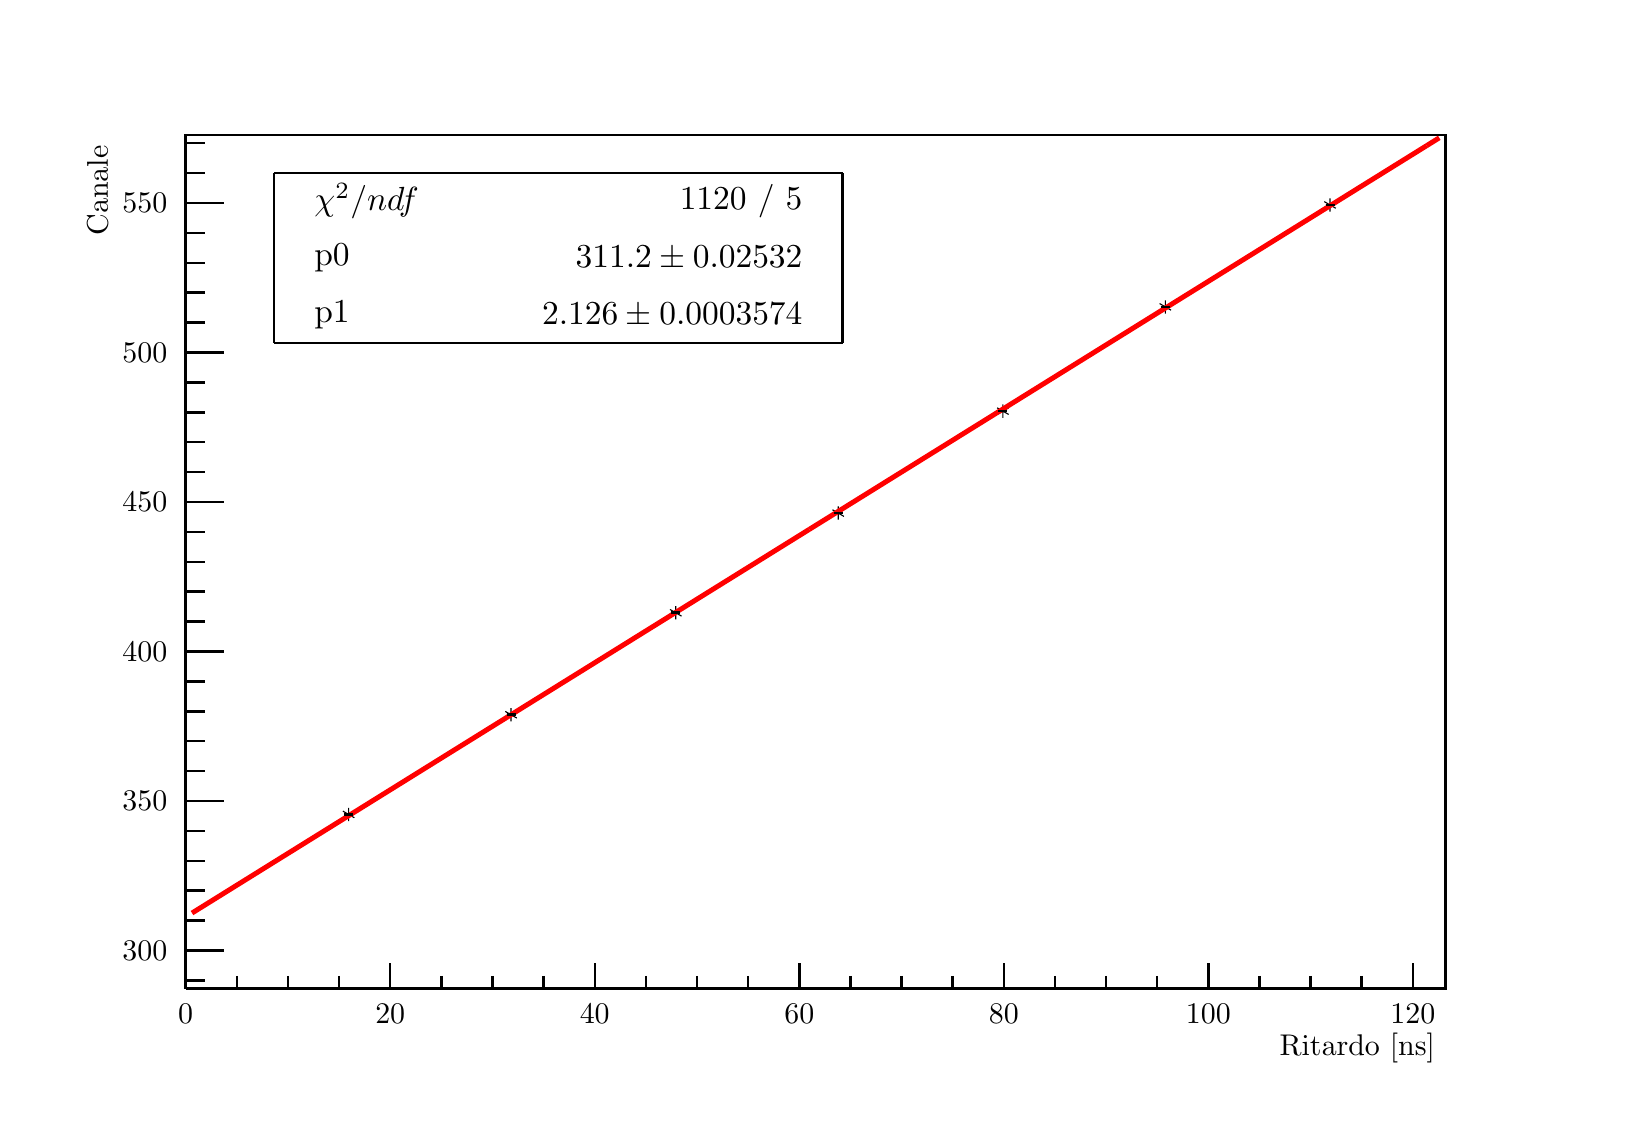
\begin{tikzpicture}
\pgfdeclareplotmark{cross} {
\pgfpathmoveto{\pgfpoint{-0.3\pgfplotmarksize}{\pgfplotmarksize}}
\pgfpathlineto{\pgfpoint{+0.3\pgfplotmarksize}{\pgfplotmarksize}}
\pgfpathlineto{\pgfpoint{+0.3\pgfplotmarksize}{0.3\pgfplotmarksize}}
\pgfpathlineto{\pgfpoint{+1\pgfplotmarksize}{0.3\pgfplotmarksize}}
\pgfpathlineto{\pgfpoint{+1\pgfplotmarksize}{-0.3\pgfplotmarksize}}
\pgfpathlineto{\pgfpoint{+0.3\pgfplotmarksize}{-0.3\pgfplotmarksize}}
\pgfpathlineto{\pgfpoint{+0.3\pgfplotmarksize}{-1.\pgfplotmarksize}}
\pgfpathlineto{\pgfpoint{-0.3\pgfplotmarksize}{-1.\pgfplotmarksize}}
\pgfpathlineto{\pgfpoint{-0.3\pgfplotmarksize}{-0.3\pgfplotmarksize}}
\pgfpathlineto{\pgfpoint{-1.\pgfplotmarksize}{-0.3\pgfplotmarksize}}
\pgfpathlineto{\pgfpoint{-1.\pgfplotmarksize}{0.3\pgfplotmarksize}}
\pgfpathlineto{\pgfpoint{-0.3\pgfplotmarksize}{0.3\pgfplotmarksize}}
\pgfpathclose
\pgfusepathqstroke
}
\pgfdeclareplotmark{cross*} {
\pgfpathmoveto{\pgfpoint{-0.3\pgfplotmarksize}{\pgfplotmarksize}}
\pgfpathlineto{\pgfpoint{+0.3\pgfplotmarksize}{\pgfplotmarksize}}
\pgfpathlineto{\pgfpoint{+0.3\pgfplotmarksize}{0.3\pgfplotmarksize}}
\pgfpathlineto{\pgfpoint{+1\pgfplotmarksize}{0.3\pgfplotmarksize}}
\pgfpathlineto{\pgfpoint{+1\pgfplotmarksize}{-0.3\pgfplotmarksize}}
\pgfpathlineto{\pgfpoint{+0.3\pgfplotmarksize}{-0.3\pgfplotmarksize}}
\pgfpathlineto{\pgfpoint{+0.3\pgfplotmarksize}{-1.\pgfplotmarksize}}
\pgfpathlineto{\pgfpoint{-0.3\pgfplotmarksize}{-1.\pgfplotmarksize}}
\pgfpathlineto{\pgfpoint{-0.3\pgfplotmarksize}{-0.3\pgfplotmarksize}}
\pgfpathlineto{\pgfpoint{-1.\pgfplotmarksize}{-0.3\pgfplotmarksize}}
\pgfpathlineto{\pgfpoint{-1.\pgfplotmarksize}{0.3\pgfplotmarksize}}
\pgfpathlineto{\pgfpoint{-0.3\pgfplotmarksize}{0.3\pgfplotmarksize}}
\pgfpathclose
\pgfusepathqfillstroke
}
\pgfdeclareplotmark{newstar} {
\pgfpathmoveto{\pgfqpoint{0pt}{\pgfplotmarksize}}
\pgfpathlineto{\pgfqpointpolar{44}{0.5\pgfplotmarksize}}
\pgfpathlineto{\pgfqpointpolar{18}{\pgfplotmarksize}}
\pgfpathlineto{\pgfqpointpolar{-20}{0.5\pgfplotmarksize}}
\pgfpathlineto{\pgfqpointpolar{-54}{\pgfplotmarksize}}
\pgfpathlineto{\pgfqpointpolar{-90}{0.5\pgfplotmarksize}}
\pgfpathlineto{\pgfqpointpolar{234}{\pgfplotmarksize}}
\pgfpathlineto{\pgfqpointpolar{198}{0.5\pgfplotmarksize}}
\pgfpathlineto{\pgfqpointpolar{162}{\pgfplotmarksize}}
\pgfpathlineto{\pgfqpointpolar{134}{0.5\pgfplotmarksize}}
\pgfpathclose
\pgfusepathqstroke
}
\pgfdeclareplotmark{newstar*} {
\pgfpathmoveto{\pgfqpoint{0pt}{\pgfplotmarksize}}
\pgfpathlineto{\pgfqpointpolar{44}{0.5\pgfplotmarksize}}
\pgfpathlineto{\pgfqpointpolar{18}{\pgfplotmarksize}}
\pgfpathlineto{\pgfqpointpolar{-20}{0.5\pgfplotmarksize}}
\pgfpathlineto{\pgfqpointpolar{-54}{\pgfplotmarksize}}
\pgfpathlineto{\pgfqpointpolar{-90}{0.5\pgfplotmarksize}}
\pgfpathlineto{\pgfqpointpolar{234}{\pgfplotmarksize}}
\pgfpathlineto{\pgfqpointpolar{198}{0.5\pgfplotmarksize}}
\pgfpathlineto{\pgfqpointpolar{162}{\pgfplotmarksize}}
\pgfpathlineto{\pgfqpointpolar{134}{0.5\pgfplotmarksize}}
\pgfpathclose
\pgfusepathqfillstroke
}
\definecolor{c}{rgb}{1,1,1};
\draw [color=c, fill=c] (0,0) rectangle (20,13.553);
\draw [color=c, fill=c] (2,1.3553) rectangle (18,12.1977);
\definecolor{c}{rgb}{0,0,0};
\draw [c,line width=0.9] (2,1.3553) -- (2,12.1977) -- (18,12.1977) -- (18,1.3553) -- (2,1.3553);
\definecolor{c}{rgb}{1,1,1};
\draw [color=c, fill=c] (2,1.3553) rectangle (18,12.1977);
\definecolor{c}{rgb}{0,0,0};
\draw [c,line width=0.9] (2,1.3553) -- (2,12.1977) -- (18,12.1977) -- (18,1.3553) -- (2,1.3553);
\draw [c,line width=0.9] (2,1.3553) -- (18,1.3553);
\draw [anchor= east] (18,0.596332) node[scale=1.08185, color=c, rotate=0]{Ritardo [ns]};
\draw [c,line width=0.9] (2,1.68057) -- (2,1.3553);
\draw [c,line width=0.9] (2.64935,1.51794) -- (2.64935,1.3553);
\draw [c,line width=0.9] (3.2987,1.51794) -- (3.2987,1.3553);
\draw [c,line width=0.9] (3.94805,1.51794) -- (3.94805,1.3553);
\draw [c,line width=0.9] (4.5974,1.68057) -- (4.5974,1.3553);
\draw [c,line width=0.9] (5.24675,1.51794) -- (5.24675,1.3553);
\draw [c,line width=0.9] (5.8961,1.51794) -- (5.8961,1.3553);
\draw [c,line width=0.9] (6.54545,1.51794) -- (6.54545,1.3553);
\draw [c,line width=0.9] (7.19481,1.68057) -- (7.19481,1.3553);
\draw [c,line width=0.9] (7.84416,1.51794) -- (7.84416,1.3553);
\draw [c,line width=0.9] (8.49351,1.51794) -- (8.49351,1.3553);
\draw [c,line width=0.9] (9.14286,1.51794) -- (9.14286,1.3553);
\draw [c,line width=0.9] (9.79221,1.68057) -- (9.79221,1.3553);
\draw [c,line width=0.9] (10.4416,1.51794) -- (10.4416,1.3553);
\draw [c,line width=0.9] (11.0909,1.51794) -- (11.0909,1.3553);
\draw [c,line width=0.9] (11.7403,1.51794) -- (11.7403,1.3553);
\draw [c,line width=0.9] (12.3896,1.68057) -- (12.3896,1.3553);
\draw [c,line width=0.9] (13.039,1.51794) -- (13.039,1.3553);
\draw [c,line width=0.9] (13.6883,1.51794) -- (13.6883,1.3553);
\draw [c,line width=0.9] (14.3377,1.51794) -- (14.3377,1.3553);
\draw [c,line width=0.9] (14.987,1.68057) -- (14.987,1.3553);
\draw [c,line width=0.9] (15.6364,1.51794) -- (15.6364,1.3553);
\draw [c,line width=0.9] (16.2857,1.51794) -- (16.2857,1.3553);
\draw [c,line width=0.9] (16.9351,1.51794) -- (16.9351,1.3553);
\draw [c,line width=0.9] (17.5844,1.68057) -- (17.5844,1.3553);
\draw [c,line width=0.9] (17.5844,1.68057) -- (17.5844,1.3553);
\draw [anchor=base] (2,0.908052) node[scale=1.08185, color=c, rotate=0]{0};
\draw [anchor=base] (4.5974,0.908052) node[scale=1.08185, color=c, rotate=0]{20};
\draw [anchor=base] (7.19481,0.908052) node[scale=1.08185, color=c, rotate=0]{40};
\draw [anchor=base] (9.79221,0.908052) node[scale=1.08185, color=c, rotate=0]{60};
\draw [anchor=base] (12.3896,0.908052) node[scale=1.08185, color=c, rotate=0]{80};
\draw [anchor=base] (14.987,0.908052) node[scale=1.08185, color=c, rotate=0]{100};
\draw [anchor=base] (17.5844,0.908052) node[scale=1.08185, color=c, rotate=0]{120};
\draw [c,line width=0.9] (2,1.3553) -- (2,12.1977);
\draw [anchor= east] (0.88,12.1977) node[scale=1.08185, color=c, rotate=90]{Canale};
\draw [c,line width=0.9] (2.48,1.83997) -- (2,1.83997);
\draw [c,line width=0.9] (2.24,2.21972) -- (2,2.21972);
\draw [c,line width=0.9] (2.24,2.59947) -- (2,2.59947);
\draw [c,line width=0.9] (2.24,2.97922) -- (2,2.97922);
\draw [c,line width=0.9] (2.24,3.35896) -- (2,3.35896);
\draw [c,line width=0.9] (2.48,3.73871) -- (2,3.73871);
\draw [c,line width=0.9] (2.24,4.11846) -- (2,4.11846);
\draw [c,line width=0.9] (2.24,4.49821) -- (2,4.49821);
\draw [c,line width=0.9] (2.24,4.87796) -- (2,4.87796);
\draw [c,line width=0.9] (2.24,5.2577) -- (2,5.2577);
\draw [c,line width=0.9] (2.48,5.63745) -- (2,5.63745);
\draw [c,line width=0.9] (2.24,6.0172) -- (2,6.0172);
\draw [c,line width=0.9] (2.24,6.39695) -- (2,6.39695);
\draw [c,line width=0.9] (2.24,6.77669) -- (2,6.77669);
\draw [c,line width=0.9] (2.24,7.15644) -- (2,7.15644);
\draw [c,line width=0.9] (2.48,7.53619) -- (2,7.53619);
\draw [c,line width=0.9] (2.24,7.91594) -- (2,7.91594);
\draw [c,line width=0.9] (2.24,8.29569) -- (2,8.29569);
\draw [c,line width=0.9] (2.24,8.67543) -- (2,8.67543);
\draw [c,line width=0.9] (2.24,9.05518) -- (2,9.05518);
\draw [c,line width=0.9] (2.48,9.43493) -- (2,9.43493);
\draw [c,line width=0.9] (2.24,9.81468) -- (2,9.81468);
\draw [c,line width=0.9] (2.24,10.1944) -- (2,10.1944);
\draw [c,line width=0.9] (2.24,10.5742) -- (2,10.5742);
\draw [c,line width=0.9] (2.24,10.9539) -- (2,10.9539);
\draw [c,line width=0.9] (2.48,11.3337) -- (2,11.3337);
\draw [c,line width=0.9] (2.48,1.83997) -- (2,1.83997);
\draw [c,line width=0.9] (2.24,1.46023) -- (2,1.46023);
\draw [c,line width=0.9] (2.48,11.3337) -- (2,11.3337);
\draw [c,line width=0.9] (2.24,11.7134) -- (2,11.7134);
\draw [c,line width=0.9] (2.24,12.0932) -- (2,12.0932);
\draw [anchor= east] (1.9,1.83997) node[scale=1.08185, color=c, rotate=0]{300};
\draw [anchor= east] (1.9,3.73871) node[scale=1.08185, color=c, rotate=0]{350};
\draw [anchor= east] (1.9,5.63745) node[scale=1.08185, color=c, rotate=0]{400};
\draw [anchor= east] (1.9,7.53619) node[scale=1.08185, color=c, rotate=0]{450};
\draw [anchor= east] (1.9,9.43493) node[scale=1.08185, color=c, rotate=0]{500};
\draw [anchor= east] (1.9,11.3337) node[scale=1.08185, color=c, rotate=0]{550};
\definecolor{c}{rgb}{1,1,1};
\draw [color=c, fill=c] (3.12321,9.55329) rectangle (10.3438,11.7114);
\definecolor{c}{rgb}{0,0,0};
\draw [c,line width=0.9] (3.12321,9.55329) -- (10.3438,9.55329);
\draw [c,line width=0.9] (10.3438,9.55329) -- (10.3438,11.7114);
\draw [c,line width=0.9] (10.3438,11.7114) -- (3.12321,11.7114);
\draw [c,line width=0.9] (3.12321,11.7114) -- (3.12321,9.55329);
\draw [anchor= west] (3.48424,11.3517) node[scale=1.20912, color=c, rotate=0]{$\chi^{2} / ndf $};
\draw [anchor= east] (9.98281,11.3517) node[scale=1.20912, color=c, rotate=0]{  1120 / 5};
\draw [anchor= west] (3.48424,10.6323) node[scale=1.20912, color=c, rotate=0]{p0       };
\draw [anchor= east] (9.98281,10.6323) node[scale=1.20912, color=c, rotate=0]{$ 311.2 \pm 0.02532$};
\draw [anchor= west] (3.48424,9.91298) node[scale=1.20912, color=c, rotate=0]{p1       };
\draw [anchor= east] (9.98281,9.91298) node[scale=1.20912, color=c, rotate=0]{$ 2.126 \pm 0.0003574$};
\foreach \P in {(4.06877,3.5681), (6.13181,4.83419), (8.2235,6.12907), (10.2865,7.39517), (12.3782,8.69004), (14.4413,10.0137), (16.5329,11.3086)}{\draw[mark options={color=c,fill=c},mark size=2.402402pt,mark=asterisk] plot coordinates {\P};}
\definecolor{c}{rgb}{1,0,0};
\draw [c,line width=1.8] (2.08,2.31566) -- (2.24,2.4151) -- (2.4,2.51455) -- (2.56,2.614) -- (2.72,2.71345) -- (2.88,2.81289) -- (3.04,2.91234) -- (3.2,3.01179) -- (3.36,3.11123) -- (3.52,3.21068) -- (3.68,3.31013) -- (3.84,3.40958) -- (4,3.50902) --
 (4.16,3.60847) -- (4.32,3.70792) -- (4.48,3.80737) -- (4.64,3.90681) -- (4.8,4.00626) -- (4.96,4.10571) -- (5.12,4.20516) -- (5.28,4.3046) -- (5.44,4.40405) -- (5.6,4.5035) -- (5.76,4.60295) -- (5.92,4.70239) -- (6.08,4.80184) -- (6.24,4.90129) --
 (6.4,5.00073) -- (6.56,5.10018) -- (6.72,5.19963) -- (6.88,5.29908) -- (7.04,5.39852) -- (7.2,5.49797) -- (7.36,5.59742) -- (7.52,5.69687) -- (7.68,5.79631) -- (7.84,5.89576) -- (8,5.99521) -- (8.16,6.09466) -- (8.32,6.1941) -- (8.48,6.29355) --
 (8.64,6.393) -- (8.8,6.49244) -- (8.96,6.59189) -- (9.12,6.69134) -- (9.28,6.79079) -- (9.44,6.89023) -- (9.6,6.98968) -- (9.76,7.08913) -- (9.92,7.18858);
\draw [c,line width=1.8] (9.92,7.18858) -- (10.08,7.28802) -- (10.24,7.38747) -- (10.4,7.48692) -- (10.56,7.58637) -- (10.72,7.68581) -- (10.88,7.78526) -- (11.04,7.88471) -- (11.2,7.98416) -- (11.36,8.0836) -- (11.52,8.18305) -- (11.68,8.2825) --
 (11.84,8.38194) -- (12,8.48139) -- (12.16,8.58084) -- (12.32,8.68029) -- (12.48,8.77973) -- (12.64,8.87918) -- (12.8,8.97863) -- (12.96,9.07808) -- (13.12,9.17752) -- (13.28,9.27697) -- (13.44,9.37642) -- (13.6,9.47587) -- (13.76,9.57531) --
 (13.92,9.67476) -- (14.08,9.77421) -- (14.24,9.87366) -- (14.4,9.9731) -- (14.56,10.0725) -- (14.72,10.172) -- (14.88,10.2714) -- (15.04,10.3709) -- (15.2,10.4703) -- (15.36,10.5698) -- (15.52,10.6692) -- (15.68,10.7687) -- (15.84,10.8681) --
 (16,10.9676) -- (16.16,11.067) -- (16.32,11.1665) -- (16.48,11.2659) -- (16.64,11.3654) -- (16.8,11.4648) -- (16.96,11.5643) -- (17.12,11.6637) -- (17.28,11.7632) -- (17.44,11.8626) -- (17.6,11.962) -- (17.76,12.0615);
\draw [c,line width=1.8] (17.76,12.0615) -- (17.92,12.1609);
\definecolor{c}{rgb}{1,1,1};
\draw [color=c, fill=c] (3.12321,9.55329) rectangle (10.3438,11.7114);
\definecolor{c}{rgb}{0,0,0};
\draw [c,line width=0.9] (3.12321,9.55329) -- (10.3438,9.55329);
\draw [c,line width=0.9] (10.3438,9.55329) -- (10.3438,11.7114);
\draw [c,line width=0.9] (10.3438,11.7114) -- (3.12321,11.7114);
\draw [c,line width=0.9] (3.12321,11.7114) -- (3.12321,9.55329);
\draw [anchor= west] (3.48424,11.3517) node[scale=1.20912, color=c, rotate=0]{$\chi^{2} / ndf $};
\draw [anchor= east] (9.98281,11.3517) node[scale=1.20912, color=c, rotate=0]{  1120 / 5};
\draw [anchor= west] (3.48424,10.6323) node[scale=1.20912, color=c, rotate=0]{p0       };
\draw [anchor= east] (9.98281,10.6323) node[scale=1.20912, color=c, rotate=0]{$ 311.2 \pm 0.02532$};
\draw [anchor= west] (3.48424,9.91298) node[scale=1.20912, color=c, rotate=0]{p1       };
\draw [anchor= east] (9.98281,9.91298) node[scale=1.20912, color=c, rotate=0]{$ 2.126 \pm 0.0003574$};
\draw [c,line width=0.9] (4.06877,3.5681) -- (4.06877,3.56923);
\draw [c,line width=0.9] (4.01146,3.56923) -- (4.12607,3.56923);
\draw [c,line width=0.9] (4.06877,3.5681) -- (4.06877,3.56696);
\draw [c,line width=0.9] (4.01146,3.56696) -- (4.12607,3.56696);
\draw [c,line width=0.9] (6.13181,4.83419) -- (6.13181,4.83533);
\draw [c,line width=0.9] (6.0745,4.83533) -- (6.18911,4.83533);
\draw [c,line width=0.9] (6.13181,4.83419) -- (6.13181,4.83305);
\draw [c,line width=0.9] (6.0745,4.83305) -- (6.18911,4.83305);
\draw [c,line width=0.9] (8.2235,6.12907) -- (8.2235,6.13021);
\draw [c,line width=0.9] (8.16619,6.13021) -- (8.2808,6.13021);
\draw [c,line width=0.9] (8.2235,6.12907) -- (8.2235,6.12793);
\draw [c,line width=0.9] (8.16619,6.12793) -- (8.2808,6.12793);
\draw [c,line width=0.9] (10.2865,7.39517) -- (10.2865,7.39631);
\draw [c,line width=0.9] (10.2292,7.39631) -- (10.3438,7.39631);
\draw [c,line width=0.9] (10.2865,7.39517) -- (10.2865,7.39403);
\draw [c,line width=0.9] (10.2292,7.39403) -- (10.3438,7.39403);
\draw [c,line width=0.9] (12.3782,8.69004) -- (12.3782,8.69156);
\draw [c,line width=0.9] (12.3209,8.69156) -- (12.4355,8.69156);
\draw [c,line width=0.9] (12.3782,8.69004) -- (12.3782,8.68852);
\draw [c,line width=0.9] (12.3209,8.68852) -- (12.4355,8.68852);
\draw [c,line width=0.9] (14.4413,10.0137) -- (14.4413,10.0148);
\draw [c,line width=0.9] (14.384,10.0148) -- (14.4986,10.0148);
\draw [c,line width=0.9] (14.4413,10.0137) -- (14.4413,10.0125);
\draw [c,line width=0.9] (14.384,10.0125) -- (14.4986,10.0125);
\draw [c,line width=0.9] (16.5329,11.3086) -- (16.5329,11.3097);
\draw [c,line width=0.9] (16.4756,11.3097) -- (16.5903,11.3097);
\draw [c,line width=0.9] (16.5329,11.3086) -- (16.5329,11.3074);
\draw [c,line width=0.9] (16.4756,11.3074) -- (16.5903,11.3074);
\end{tikzpicture}

%Inserire regressione lineare della calibrazione temporale dell'apparato strumentale


Una volta calibrato tutto il sistema di acquisizione, si è arrivati al vero e proprio studio del positronio: in particolare si vuole misurare il rapporto tra il decadimento
a due e a tre fotoni del positronio e la distribuzione temporale degli eventi.\\

\FloatBarrier
\subsection{Decadimento a due fotoni}

Si inizi dal decadimento a due fotoni: la misura è stata fatta andando a registrare gli spettri dei tre rivelatori complanari assieme allo spettro del TAC. Il
trigger è stato impostato sulla coincidenza tra R1 ed R2, ed a tale valore è stato impostato anche lo stop del TAC, mentre lo start del TAC è stato dato da R4 che visualizza
un segnale (si ricorda che la soglia di R4 è stata regolata in modo da vedere solo segnali di energia uguale o superiore al fotopicco da 1275~keV). Gli spettri calibrati che
si sono visti si possono vedere nella Figura \ref{gr:180_misura1_spettricalibrati}.\\
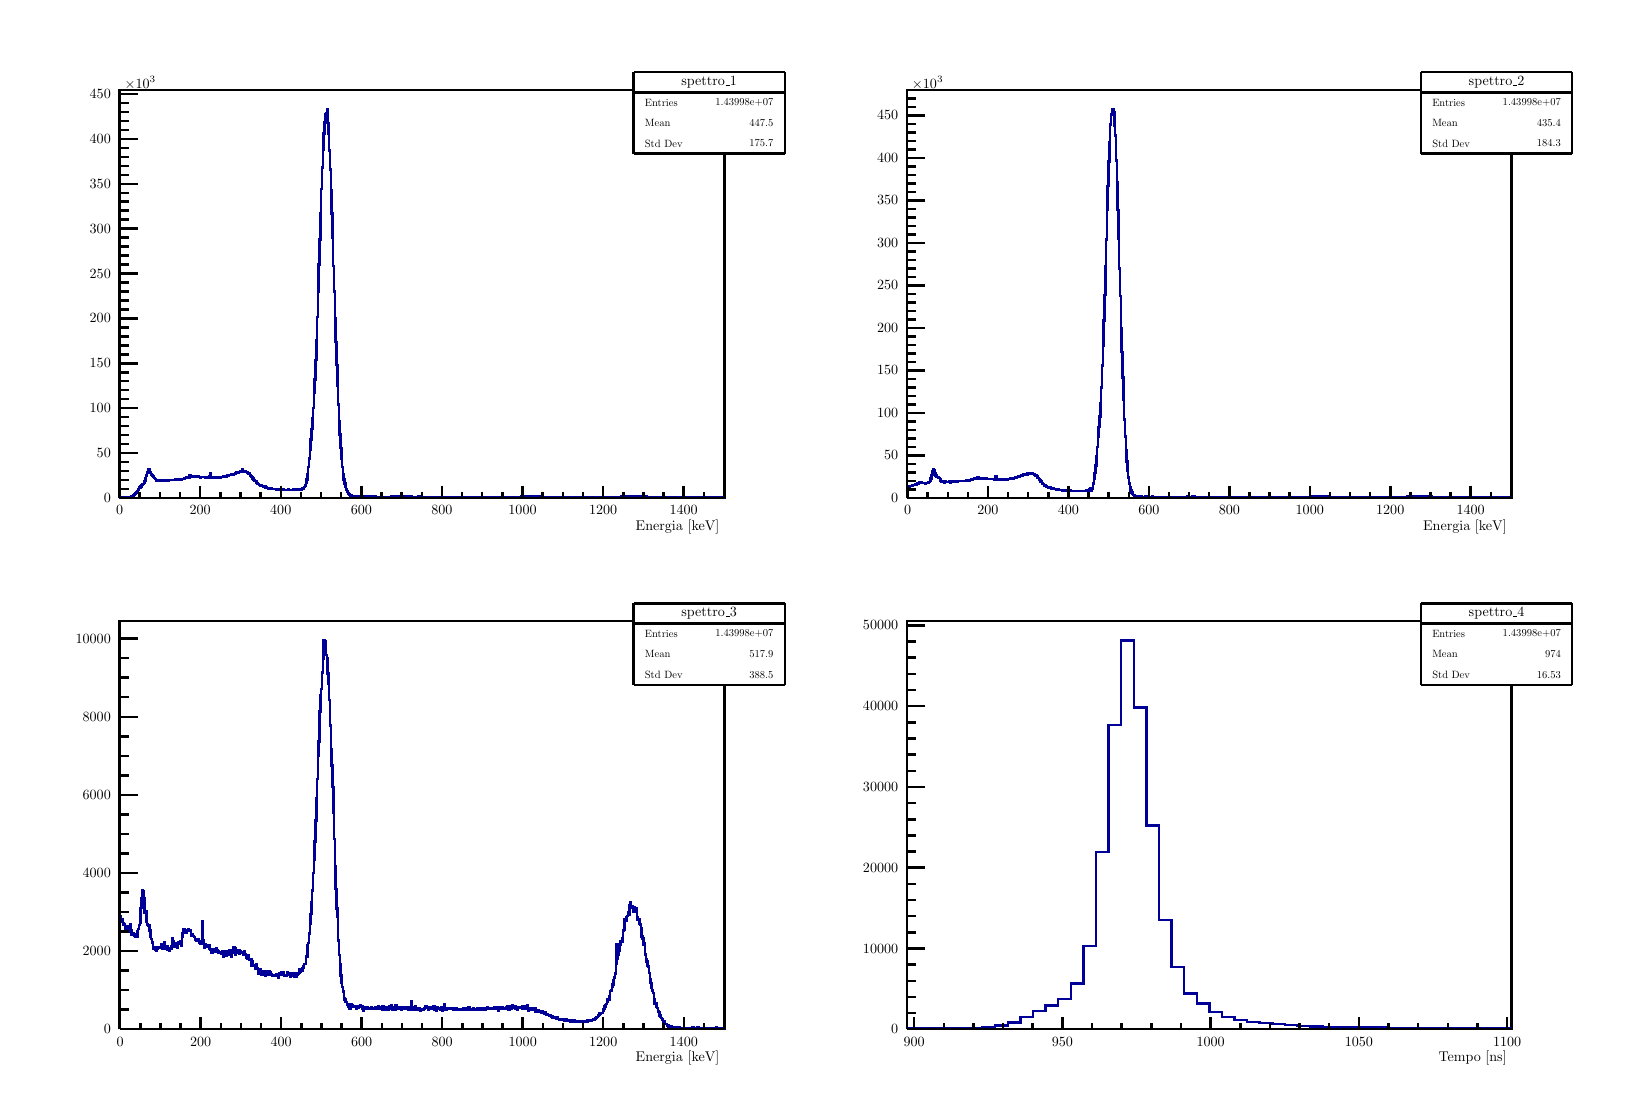
\begin{tikzpicture}
\pgfdeclareplotmark{cross} {
\pgfpathmoveto{\pgfpoint{-0.3\pgfplotmarksize}{\pgfplotmarksize}}
\pgfpathlineto{\pgfpoint{+0.3\pgfplotmarksize}{\pgfplotmarksize}}
\pgfpathlineto{\pgfpoint{+0.3\pgfplotmarksize}{0.3\pgfplotmarksize}}
\pgfpathlineto{\pgfpoint{+1\pgfplotmarksize}{0.3\pgfplotmarksize}}
\pgfpathlineto{\pgfpoint{+1\pgfplotmarksize}{-0.3\pgfplotmarksize}}
\pgfpathlineto{\pgfpoint{+0.3\pgfplotmarksize}{-0.3\pgfplotmarksize}}
\pgfpathlineto{\pgfpoint{+0.3\pgfplotmarksize}{-1.\pgfplotmarksize}}
\pgfpathlineto{\pgfpoint{-0.3\pgfplotmarksize}{-1.\pgfplotmarksize}}
\pgfpathlineto{\pgfpoint{-0.3\pgfplotmarksize}{-0.3\pgfplotmarksize}}
\pgfpathlineto{\pgfpoint{-1.\pgfplotmarksize}{-0.3\pgfplotmarksize}}
\pgfpathlineto{\pgfpoint{-1.\pgfplotmarksize}{0.3\pgfplotmarksize}}
\pgfpathlineto{\pgfpoint{-0.3\pgfplotmarksize}{0.3\pgfplotmarksize}}
\pgfpathclose
\pgfusepathqstroke
}
\pgfdeclareplotmark{cross*} {
\pgfpathmoveto{\pgfpoint{-0.3\pgfplotmarksize}{\pgfplotmarksize}}
\pgfpathlineto{\pgfpoint{+0.3\pgfplotmarksize}{\pgfplotmarksize}}
\pgfpathlineto{\pgfpoint{+0.3\pgfplotmarksize}{0.3\pgfplotmarksize}}
\pgfpathlineto{\pgfpoint{+1\pgfplotmarksize}{0.3\pgfplotmarksize}}
\pgfpathlineto{\pgfpoint{+1\pgfplotmarksize}{-0.3\pgfplotmarksize}}
\pgfpathlineto{\pgfpoint{+0.3\pgfplotmarksize}{-0.3\pgfplotmarksize}}
\pgfpathlineto{\pgfpoint{+0.3\pgfplotmarksize}{-1.\pgfplotmarksize}}
\pgfpathlineto{\pgfpoint{-0.3\pgfplotmarksize}{-1.\pgfplotmarksize}}
\pgfpathlineto{\pgfpoint{-0.3\pgfplotmarksize}{-0.3\pgfplotmarksize}}
\pgfpathlineto{\pgfpoint{-1.\pgfplotmarksize}{-0.3\pgfplotmarksize}}
\pgfpathlineto{\pgfpoint{-1.\pgfplotmarksize}{0.3\pgfplotmarksize}}
\pgfpathlineto{\pgfpoint{-0.3\pgfplotmarksize}{0.3\pgfplotmarksize}}
\pgfpathclose
\pgfusepathqfillstroke
}
\pgfdeclareplotmark{newstar} {
\pgfpathmoveto{\pgfqpoint{0pt}{\pgfplotmarksize}}
\pgfpathlineto{\pgfqpointpolar{44}{0.5\pgfplotmarksize}}
\pgfpathlineto{\pgfqpointpolar{18}{\pgfplotmarksize}}
\pgfpathlineto{\pgfqpointpolar{-20}{0.5\pgfplotmarksize}}
\pgfpathlineto{\pgfqpointpolar{-54}{\pgfplotmarksize}}
\pgfpathlineto{\pgfqpointpolar{-90}{0.5\pgfplotmarksize}}
\pgfpathlineto{\pgfqpointpolar{234}{\pgfplotmarksize}}
\pgfpathlineto{\pgfqpointpolar{198}{0.5\pgfplotmarksize}}
\pgfpathlineto{\pgfqpointpolar{162}{\pgfplotmarksize}}
\pgfpathlineto{\pgfqpointpolar{134}{0.5\pgfplotmarksize}}
\pgfpathclose
\pgfusepathqstroke
}
\pgfdeclareplotmark{newstar*} {
\pgfpathmoveto{\pgfqpoint{0pt}{\pgfplotmarksize}}
\pgfpathlineto{\pgfqpointpolar{44}{0.5\pgfplotmarksize}}
\pgfpathlineto{\pgfqpointpolar{18}{\pgfplotmarksize}}
\pgfpathlineto{\pgfqpointpolar{-20}{0.5\pgfplotmarksize}}
\pgfpathlineto{\pgfqpointpolar{-54}{\pgfplotmarksize}}
\pgfpathlineto{\pgfqpointpolar{-90}{0.5\pgfplotmarksize}}
\pgfpathlineto{\pgfqpointpolar{234}{\pgfplotmarksize}}
\pgfpathlineto{\pgfqpointpolar{198}{0.5\pgfplotmarksize}}
\pgfpathlineto{\pgfqpointpolar{162}{\pgfplotmarksize}}
\pgfpathlineto{\pgfqpointpolar{134}{0.5\pgfplotmarksize}}
\pgfpathclose
\pgfusepathqfillstroke
}
\definecolor{c}{rgb}{1,1,1};
\draw [color=c, fill=c] (0,0) rectangle (20,13.4957);
\draw [color=c, fill=c] (0.2,6.88281) rectangle (9.8,13.3607);
\draw [color=c, fill=c] (1.16,7.5306) rectangle (8.84,12.713);
\definecolor{c}{rgb}{0,0,0};
\draw [c,line width=0.9] (1.16,7.5306) -- (1.16,12.713) -- (8.84,12.713) -- (8.84,7.5306) -- (1.16,7.5306);
\definecolor{c}{rgb}{1,1,1};
\draw [color=c, fill=c] (1.16,7.5306) rectangle (8.84,12.713);
\definecolor{c}{rgb}{0,0,0};
\draw [c,line width=0.9] (1.16,7.5306) -- (1.16,12.713) -- (8.84,12.713) -- (8.84,7.5306) -- (1.16,7.5306);
\definecolor{c}{rgb}{0,0,0.6};
\draw [c,line width=0.9] (1.16,7.5364) -- (1.17024,7.5364) -- (1.17024,7.53605) -- (1.18048,7.53605) -- (1.18048,7.5362) -- (1.19072,7.5362) -- (1.19072,7.5368) -- (1.20096,7.5368) -- (1.20096,7.53644) -- (1.2112,7.53644) -- (1.2112,7.53628) --
 (1.22144,7.53628) -- (1.22144,7.53624) -- (1.23168,7.53624) -- (1.23168,7.53612) -- (1.24192,7.53612) -- (1.24192,7.5367) -- (1.25216,7.5367) -- (1.25216,7.53694) -- (1.2624,7.53694) -- (1.2624,7.53729) -- (1.27264,7.53729) -- (1.27264,7.53766) --
 (1.28288,7.53766) -- (1.28288,7.53936) -- (1.29312,7.53936) -- (1.29312,7.54127) -- (1.30336,7.54127) -- (1.30336,7.54323) -- (1.3136,7.54323) -- (1.3136,7.54843) -- (1.32384,7.54843) -- (1.32384,7.55373) -- (1.33408,7.55373) -- (1.33408,7.56328) --
 (1.34432,7.56328) -- (1.34432,7.57366) -- (1.35456,7.57366) -- (1.35456,7.58531) -- (1.3648,7.58531) -- (1.3648,7.59586) -- (1.37504,7.59586) -- (1.37504,7.60858) -- (1.38528,7.60858) -- (1.38528,7.6214) -- (1.39552,7.6214) -- (1.39552,7.63473) --
 (1.40576,7.63473) -- (1.40576,7.65766) -- (1.416,7.65766) -- (1.416,7.66396) -- (1.42624,7.66396) -- (1.42624,7.67555) -- (1.43648,7.67555) -- (1.43648,7.68812) -- (1.44672,7.68812) -- (1.44672,7.70064) -- (1.45696,7.70064) -- (1.45696,7.70882) --
 (1.4672,7.70882) -- (1.4672,7.72677) -- (1.47744,7.72677) -- (1.47744,7.74613) -- (1.48768,7.74613) -- (1.48768,7.77516) -- (1.49792,7.77516) -- (1.49792,7.81677) -- (1.50816,7.81677) -- (1.50816,7.85267) -- (1.5184,7.85267) -- (1.5184,7.87905) --
 (1.52864,7.87905) -- (1.52864,7.88969) -- (1.53888,7.88969) -- (1.53888,7.87813) -- (1.54912,7.87813) -- (1.54912,7.85192) -- (1.55936,7.85192) -- (1.55936,7.83017) -- (1.5696,7.83017) -- (1.5696,7.81796) -- (1.57984,7.81796) -- (1.57984,7.81139) --
 (1.59008,7.81139) -- (1.59008,7.79992) -- (1.60032,7.79992) -- (1.60032,7.78658) -- (1.61056,7.78658) -- (1.61056,7.77201) -- (1.6208,7.77201) -- (1.6208,7.75849) -- (1.63104,7.75849) -- (1.63104,7.75268) -- (1.64128,7.75268) -- (1.64128,7.74719) --
 (1.65152,7.74719) -- (1.65152,7.74751) -- (1.66176,7.74751) -- (1.66176,7.75233) -- (1.672,7.75233) -- (1.672,7.74833) -- (1.68224,7.74833) -- (1.68224,7.74614) -- (1.69248,7.74614) -- (1.69248,7.75415) -- (1.70272,7.75415) -- (1.70272,7.74768) --
 (1.71296,7.74768) -- (1.71296,7.74738) -- (1.7232,7.74738) -- (1.7232,7.75128) -- (1.73344,7.75128) -- (1.73344,7.75386) -- (1.74368,7.75386) -- (1.74368,7.75019) -- (1.75392,7.75019) -- (1.75392,7.75144) -- (1.76416,7.75144) -- (1.76416,7.75033) --
 (1.7744,7.75033) -- (1.7744,7.75338) -- (1.78464,7.75338) -- (1.78464,7.75628) -- (1.79488,7.75628) -- (1.79488,7.75563) -- (1.80512,7.75563) -- (1.80512,7.75503) -- (1.81536,7.75503) -- (1.81536,7.75533) -- (1.8256,7.75533) -- (1.8256,7.75991) --
 (1.83584,7.75991) -- (1.83584,7.75742) -- (1.84608,7.75742) -- (1.84608,7.75987) -- (1.85632,7.75987) -- (1.85632,7.75996) -- (1.86656,7.75996) -- (1.86656,7.76137) -- (1.8768,7.76137) -- (1.8768,7.76039) -- (1.88704,7.76039) -- (1.88704,7.76283) --
 (1.89728,7.76283) -- (1.89728,7.76413) -- (1.90752,7.76413) -- (1.90752,7.7624) -- (1.91776,7.7624) -- (1.91776,7.76297) -- (1.928,7.76297) -- (1.928,7.76382) -- (1.93824,7.76382) -- (1.93824,7.76554) -- (1.94848,7.76554) -- (1.94848,7.76949) --
 (1.95872,7.76949) -- (1.95872,7.77002) -- (1.96896,7.77002) -- (1.96896,7.7731) -- (1.9792,7.7731) -- (1.9792,7.77599) -- (1.98944,7.77599) -- (1.98944,7.78551) -- (1.99968,7.78551) -- (1.99968,7.78256) -- (2.00992,7.78256) -- (2.00992,7.78823) --
 (2.02016,7.78823) -- (2.02016,7.79137) -- (2.0304,7.79137) -- (2.0304,7.79314) -- (2.04064,7.79314) -- (2.04064,7.79204) -- (2.05088,7.79204) -- (2.05088,7.81799) -- (2.06112,7.81799) -- (2.06112,7.80498) -- (2.07136,7.80498) -- (2.07136,7.80196) --
 (2.0816,7.80196) -- (2.0816,7.79966) -- (2.09184,7.79966) -- (2.09184,7.79977) -- (2.10208,7.79977) -- (2.10208,7.79586) -- (2.11232,7.79586) -- (2.11232,7.79401) -- (2.12256,7.79401) -- (2.12256,7.7972) -- (2.1328,7.7972) -- (2.1328,7.7997) --
 (2.14304,7.7997) -- (2.14304,7.79685) -- (2.15328,7.79685) -- (2.15328,7.79965) -- (2.16352,7.79965) -- (2.16352,7.79342) -- (2.17376,7.79342) -- (2.17376,7.79378) -- (2.184,7.79378) -- (2.184,7.79051) -- (2.19424,7.79051) -- (2.19424,7.79365) --
 (2.20448,7.79365) -- (2.20448,7.79313) -- (2.21472,7.79313) -- (2.21472,7.79656) -- (2.22496,7.79656) -- (2.22496,7.79677) -- (2.2352,7.79677) -- (2.2352,7.79662) -- (2.24544,7.79662) -- (2.24544,7.79196) -- (2.25568,7.79196) -- (2.25568,7.79328) --
 (2.26592,7.79328) -- (2.26592,7.79074) -- (2.27616,7.79074) -- (2.27616,7.79026) -- (2.2864,7.79026) -- (2.2864,7.78822) -- (2.29664,7.78822) -- (2.29664,7.80576) -- (2.30688,7.80576) -- (2.30688,7.84866) -- (2.31712,7.84866) -- (2.31712,7.79294) --
 (2.32736,7.79294) -- (2.32736,7.78731) -- (2.3376,7.78731) -- (2.3376,7.78865) -- (2.34784,7.78865) -- (2.34784,7.7857) -- (2.35808,7.7857) -- (2.35808,7.7864) -- (2.36832,7.7864) -- (2.36832,7.78583) -- (2.37856,7.78583) -- (2.37856,7.78765) --
 (2.3888,7.78765) -- (2.3888,7.78898) -- (2.39904,7.78898) -- (2.39904,7.78692) -- (2.40928,7.78692) -- (2.40928,7.78766) -- (2.41952,7.78766) -- (2.41952,7.78848) -- (2.42976,7.78848) -- (2.42976,7.78966) -- (2.44,7.78966) -- (2.44,7.78873) --
 (2.45024,7.78873) -- (2.45024,7.79501) -- (2.46048,7.79501) -- (2.46048,7.79658) -- (2.47072,7.79658) -- (2.47072,7.79681) -- (2.48096,7.79681) -- (2.48096,7.8041) -- (2.4912,7.8041) -- (2.4912,7.80223) -- (2.50144,7.80223) -- (2.50144,7.80654) --
 (2.51168,7.80654) -- (2.51168,7.80555) -- (2.52192,7.80555) -- (2.52192,7.81039) -- (2.53216,7.81039) -- (2.53216,7.81441) -- (2.5424,7.81441) -- (2.5424,7.81704) -- (2.55264,7.81704) -- (2.55264,7.82219) -- (2.56288,7.82219) -- (2.56288,7.81996) --
 (2.57312,7.81996) -- (2.57312,7.82198) -- (2.58336,7.82198) -- (2.58336,7.82994) -- (2.5936,7.82994) -- (2.5936,7.82904) -- (2.60384,7.82904) -- (2.60384,7.83379) -- (2.61408,7.83379) -- (2.61408,7.83624) -- (2.62432,7.83624) -- (2.62432,7.84363) --
 (2.63456,7.84363) -- (2.63456,7.84504) -- (2.6448,7.84504) -- (2.6448,7.85615) -- (2.65504,7.85615) -- (2.65504,7.85098) -- (2.66528,7.85098) -- (2.66528,7.85285) -- (2.67552,7.85285) -- (2.67552,7.85738) -- (2.68576,7.85738) -- (2.68576,7.86102) --
 (2.696,7.86102) -- (2.696,7.86649) -- (2.70624,7.86649) -- (2.70624,7.87116) -- (2.71648,7.87116) -- (2.71648,7.89144) -- (2.72672,7.89144) -- (2.72672,7.86886) -- (2.73696,7.86886) -- (2.73696,7.86634) -- (2.7472,7.86634) -- (2.7472,7.86396) --
 (2.75744,7.86396) -- (2.75744,7.85897) -- (2.76768,7.85897) -- (2.76768,7.85809) -- (2.77792,7.85809) -- (2.77792,7.85125) -- (2.78816,7.85125) -- (2.78816,7.84979) -- (2.7984,7.84979) -- (2.7984,7.83974) -- (2.80864,7.83974) -- (2.80864,7.83167) --
 (2.81888,7.83167) -- (2.81888,7.81756) -- (2.82912,7.81756) -- (2.82912,7.80468) -- (2.83936,7.80468) -- (2.83936,7.79139) -- (2.8496,7.79139) -- (2.8496,7.77901) -- (2.85984,7.77901) -- (2.85984,7.76752) -- (2.87008,7.76752) -- (2.87008,7.75396) --
 (2.88032,7.75396) -- (2.88032,7.7467) -- (2.89056,7.7467) -- (2.89056,7.73817) -- (2.9008,7.73817) -- (2.9008,7.72145) -- (2.91104,7.72145) -- (2.91104,7.7136) -- (2.92128,7.7136) -- (2.92128,7.70407) -- (2.93152,7.70407) -- (2.93152,7.69766) --
 (2.94176,7.69766) -- (2.94176,7.69127) -- (2.952,7.69127) -- (2.952,7.6863) -- (2.96224,7.6863) -- (2.96224,7.68109) -- (2.97248,7.68109) -- (2.97248,7.67896) -- (2.98272,7.67896) -- (2.98272,7.66986) -- (2.99296,7.66986) -- (2.99296,7.66775) --
 (3.0032,7.66775) -- (3.0032,7.67319) -- (3.01344,7.67319) -- (3.01344,7.66322) -- (3.02368,7.66322) -- (3.02368,7.65938) -- (3.03392,7.65938) -- (3.03392,7.65735) -- (3.04416,7.65735) -- (3.04416,7.65392) -- (3.0544,7.65392) -- (3.0544,7.65289) --
 (3.06464,7.65289) -- (3.06464,7.65224) -- (3.07488,7.65224) -- (3.07488,7.6519) -- (3.08512,7.6519) -- (3.08512,7.64716) -- (3.09536,7.64716) -- (3.09536,7.64573) -- (3.1056,7.64573) -- (3.1056,7.6454) -- (3.11584,7.6454) -- (3.11584,7.64463) --
 (3.12608,7.64463) -- (3.12608,7.64152) -- (3.13632,7.64152) -- (3.13632,7.64421) -- (3.14656,7.64421) -- (3.14656,7.63968) -- (3.1568,7.63968) -- (3.1568,7.63883) -- (3.16704,7.63883) -- (3.16704,7.63795) -- (3.17728,7.63795) -- (3.17728,7.63608) --
 (3.18752,7.63608) -- (3.18752,7.63635) -- (3.19776,7.63635) -- (3.19776,7.63654) -- (3.208,7.63654) -- (3.208,7.63619) -- (3.21824,7.63619) -- (3.21824,7.63444) -- (3.22848,7.63444) -- (3.22848,7.63799) -- (3.23872,7.63799) -- (3.23872,7.63439) --
 (3.24896,7.63439) -- (3.24896,7.63419) -- (3.2592,7.63419) -- (3.2592,7.63305) -- (3.26944,7.63305) -- (3.26944,7.63043) -- (3.27968,7.63043) -- (3.27968,7.63137) -- (3.28992,7.63137) -- (3.28992,7.63027) -- (3.30016,7.63027) -- (3.30016,7.63593) --
 (3.3104,7.63593) -- (3.3104,7.62962) -- (3.32064,7.62962) -- (3.32064,7.63053) -- (3.33088,7.63053) -- (3.33088,7.62909) -- (3.34112,7.62909) -- (3.34112,7.62983) -- (3.35136,7.62983) -- (3.35136,7.63177) -- (3.3616,7.63177) -- (3.3616,7.63874) --
 (3.37184,7.63874) -- (3.37184,7.63143) -- (3.38208,7.63143) -- (3.38208,7.62913) -- (3.39232,7.62913) -- (3.39232,7.63139) -- (3.40256,7.63139) -- (3.40256,7.63491) -- (3.4128,7.63491) -- (3.4128,7.6321) -- (3.42304,7.6321) -- (3.42304,7.63198) --
 (3.43328,7.63198) -- (3.43328,7.63235) -- (3.44352,7.63235) -- (3.44352,7.63563) -- (3.45376,7.63563) -- (3.45376,7.63698) -- (3.464,7.63698) -- (3.464,7.64022) -- (3.47424,7.64022) -- (3.47424,7.64238) -- (3.48448,7.64238) -- (3.48448,7.64998) --
 (3.49472,7.64998) -- (3.49472,7.65633) -- (3.50496,7.65633) -- (3.50496,7.66883) -- (3.5152,7.66883) -- (3.5152,7.68789) -- (3.52544,7.68789) -- (3.52544,7.71678) -- (3.53568,7.71678) -- (3.53568,7.76707) -- (3.54592,7.76707) -- (3.54592,7.83392) --
 (3.55616,7.83392) -- (3.55616,7.92303) -- (3.5664,7.92303) -- (3.5664,8.03293) -- (3.57664,8.03293) -- (3.57664,8.14769) -- (3.58688,8.14769) -- (3.58688,8.27001) -- (3.59712,8.27001) -- (3.59712,8.40406) -- (3.60736,8.40406) -- (3.60736,8.53699) --
 (3.6176,8.53699) -- (3.6176,8.67447) -- (3.62784,8.67447) -- (3.62784,8.86193) -- (3.63808,8.86193) -- (3.63808,9.03467) -- (3.64832,9.03467) -- (3.64832,9.27887) -- (3.65856,9.27887) -- (3.65856,9.53418) -- (3.6688,9.53418) -- (3.6688,9.82693) --
 (3.67904,9.82693) -- (3.67904,10.151) -- (3.68928,10.151) -- (3.68928,10.4968) -- (3.69952,10.4968) -- (3.69952,10.8153) -- (3.70976,10.8153) -- (3.70976,11.1422) -- (3.72,11.1422) -- (3.72,11.4539) -- (3.73024,11.4539) -- (3.73024,11.7274) --
 (3.74048,11.7274) -- (3.74048,11.9575) -- (3.75072,11.9575) -- (3.75072,12.1565) -- (3.76096,12.1565) -- (3.76096,12.3026) -- (3.7712,12.3026) -- (3.7712,12.4086) -- (3.78144,12.4086) -- (3.78144,12.4176) -- (3.79168,12.4176) -- (3.79168,12.4662) --
 (3.80192,12.4662) -- (3.80192,12.292) -- (3.81216,12.292) -- (3.81216,12.1507) -- (3.8224,12.1507) -- (3.8224,11.9398) -- (3.83264,11.9398) -- (3.83264,11.7005) -- (3.84288,11.7005) -- (3.84288,11.4345) -- (3.85312,11.4345) -- (3.85312,11.1421) --
 (3.86336,11.1421) -- (3.86336,10.8313) -- (3.8736,10.8313) -- (3.8736,10.4736) -- (3.88384,10.4736) -- (3.88384,10.15) -- (3.89408,10.15) -- (3.89408,9.81365) -- (3.90432,9.81365) -- (3.90432,9.5096) -- (3.91456,9.5096) -- (3.91456,9.21815) --
 (3.9248,9.21815) -- (3.9248,8.94948) -- (3.93504,8.94948) -- (3.93504,8.71816) -- (3.94528,8.71816) -- (3.94528,8.50709) -- (3.95552,8.50709) -- (3.95552,8.33412) -- (3.96576,8.33412) -- (3.96576,8.16604) -- (3.976,8.16604) -- (3.976,8.02643) --
 (3.98624,8.02643) -- (3.98624,7.92161) -- (3.99648,7.92161) -- (3.99648,7.83511) -- (4.00672,7.83511) -- (4.00672,7.76705) -- (4.01696,7.76705) -- (4.01696,7.71319) -- (4.0272,7.71319) -- (4.0272,7.67633) -- (4.03744,7.67633) -- (4.03744,7.63535) --
 (4.04768,7.63535) -- (4.04768,7.61178) -- (4.05792,7.61178) -- (4.05792,7.59293) -- (4.06816,7.59293) -- (4.06816,7.57856) -- (4.0784,7.57856) -- (4.0784,7.57008) -- (4.08864,7.57008) -- (4.08864,7.56274) -- (4.09888,7.56274) -- (4.09888,7.55895) --
 (4.10912,7.55895) -- (4.10912,7.55491) -- (4.11936,7.55491) -- (4.11936,7.5522) -- (4.1296,7.5522) -- (4.1296,7.55037) -- (4.13984,7.55037) -- (4.13984,7.54904) -- (4.15008,7.54904) -- (4.15008,7.54796) -- (4.16032,7.54796) -- (4.16032,7.54678) --
 (4.17056,7.54678) -- (4.17056,7.54769) -- (4.1808,7.54769) -- (4.1808,7.5481) -- (4.19104,7.5481) -- (4.19104,7.54698) -- (4.20128,7.54698) -- (4.20128,7.54634) -- (4.21152,7.54634) -- (4.21152,7.54701) -- (4.22176,7.54701) -- (4.22176,7.54578) --
 (4.232,7.54578) -- (4.232,7.54625) -- (4.24224,7.54625) -- (4.24224,7.54548) -- (4.25248,7.54548) -- (4.25248,7.54647) -- (4.26272,7.54647) -- (4.26272,7.54644) -- (4.27296,7.54644) -- (4.27296,7.54627) -- (4.2832,7.54627) -- (4.2832,7.54595) --
 (4.29344,7.54595) -- (4.29344,7.54557) -- (4.30368,7.54557) -- (4.30368,7.54564) -- (4.31392,7.54564) -- (4.31392,7.5455) -- (4.32416,7.5455) -- (4.32416,7.54487) -- (4.3344,7.54487) -- (4.3344,7.54516) -- (4.34464,7.54516) -- (4.34464,7.5457) --
 (4.35488,7.5457) -- (4.35488,7.54543) -- (4.36512,7.54543) -- (4.36512,7.54536) -- (4.37536,7.54536) -- (4.37536,7.54564) -- (4.3856,7.54564) -- (4.3856,7.54503) -- (4.39584,7.54503) -- (4.39584,7.54451) -- (4.40608,7.54451) -- (4.40608,7.54542) --
 (4.41632,7.54542) -- (4.41632,7.54413) -- (4.42656,7.54413) -- (4.42656,7.54459) -- (4.4368,7.54459) -- (4.4368,7.54505) -- (4.44704,7.54505) -- (4.44704,7.54475) -- (4.45728,7.54475) -- (4.45728,7.54411) -- (4.46752,7.54411) -- (4.46752,7.54507) --
 (4.47776,7.54507) -- (4.47776,7.54483) -- (4.488,7.54483) -- (4.488,7.54482) -- (4.49824,7.54482) -- (4.49824,7.54458) -- (4.50848,7.54458) -- (4.50848,7.54469) -- (4.51872,7.54469) -- (4.51872,7.5452) -- (4.52896,7.5452) -- (4.52896,7.54478) --
 (4.5392,7.54478) -- (4.5392,7.54488) -- (4.54944,7.54488) -- (4.54944,7.54454) -- (4.55968,7.54454) -- (4.55968,7.5443) -- (4.56992,7.5443) -- (4.56992,7.54533) -- (4.58016,7.54533) -- (4.58016,7.54475) -- (4.5904,7.54475) -- (4.5904,7.54475) --
 (4.60064,7.54475) -- (4.60064,7.54537) -- (4.61088,7.54537) -- (4.61088,7.54559) -- (4.62112,7.54559) -- (4.62112,7.54484) -- (4.63136,7.54484) -- (4.63136,7.5452) -- (4.6416,7.5452) -- (4.6416,7.5463) -- (4.65184,7.5463) -- (4.65184,7.54575) --
 (4.66208,7.54575) -- (4.66208,7.54552) -- (4.67232,7.54552) -- (4.67232,7.54789) -- (4.68256,7.54789) -- (4.68256,7.54526) -- (4.6928,7.54526) -- (4.6928,7.54588) -- (4.70304,7.54588) -- (4.70304,7.54562) -- (4.71328,7.54562) -- (4.71328,7.54631) --
 (4.72352,7.54631) -- (4.72352,7.54541) -- (4.73376,7.54541) -- (4.73376,7.54642) -- (4.744,7.54642) -- (4.744,7.54548) -- (4.75424,7.54548) -- (4.75424,7.54605) -- (4.76448,7.54605) -- (4.76448,7.54562) -- (4.77472,7.54562) -- (4.77472,7.54609) --
 (4.78496,7.54609) -- (4.78496,7.5459) -- (4.7952,7.5459) -- (4.7952,7.54615) -- (4.80544,7.54615) -- (4.80544,7.54543) -- (4.81568,7.54543) -- (4.81568,7.54507) -- (4.82592,7.54507) -- (4.82592,7.54616) -- (4.83616,7.54616) -- (4.83616,7.54595) --
 (4.8464,7.54595) -- (4.8464,7.54489) -- (4.85664,7.54489) -- (4.85664,7.5456) -- (4.86688,7.5456) -- (4.86688,7.54502) -- (4.87712,7.54502) -- (4.87712,7.5447) -- (4.88736,7.5447) -- (4.88736,7.54515) -- (4.8976,7.54515) -- (4.8976,7.54474) --
 (4.90784,7.54474) -- (4.90784,7.54423) -- (4.91808,7.54423) -- (4.91808,7.54507) -- (4.92832,7.54507) -- (4.92832,7.5435) -- (4.93856,7.5435) -- (4.93856,7.54493) -- (4.9488,7.54493) -- (4.9488,7.54472) -- (4.95904,7.54472) -- (4.95904,7.54779) --
 (4.96928,7.54779) -- (4.96928,7.54483) -- (4.97952,7.54483) -- (4.97952,7.54372) -- (4.98976,7.54372) -- (4.98976,7.54455) -- (5,7.54455) -- (5,7.54352) -- (5.01024,7.54352) -- (5.01024,7.54365) -- (5.02048,7.54365) -- (5.02048,7.54422) --
 (5.03072,7.54422) -- (5.03072,7.54308) -- (5.04096,7.54308) -- (5.04096,7.54366) -- (5.0512,7.54366) -- (5.0512,7.54371) -- (5.06144,7.54371) -- (5.06144,7.54325) -- (5.07168,7.54325) -- (5.07168,7.54376) -- (5.08192,7.54376) -- (5.08192,7.54409) --
 (5.09216,7.54409) -- (5.09216,7.54378) -- (5.1024,7.54378) -- (5.1024,7.54344) -- (5.11264,7.54344) -- (5.11264,7.54332) -- (5.12288,7.54332) -- (5.12288,7.54381) -- (5.13312,7.54381) -- (5.13312,7.54409) -- (5.14336,7.54409) -- (5.14336,7.54363) --
 (5.1536,7.54363) -- (5.1536,7.54369) -- (5.16384,7.54369) -- (5.16384,7.54328) -- (5.17408,7.54328) -- (5.17408,7.54346) -- (5.18432,7.54346) -- (5.18432,7.54345) -- (5.19456,7.54345) -- (5.19456,7.54292) -- (5.2048,7.54292) -- (5.2048,7.5436) --
 (5.21504,7.5436) -- (5.21504,7.54328) -- (5.22528,7.54328) -- (5.22528,7.54393) -- (5.23552,7.54393) -- (5.23552,7.54223) -- (5.24576,7.54223) -- (5.24576,7.54353) -- (5.256,7.54353) -- (5.256,7.54272) -- (5.26624,7.54272) -- (5.26624,7.543) --
 (5.27648,7.543) -- (5.27648,7.54376) -- (5.28672,7.54376) -- (5.28672,7.54262) -- (5.29696,7.54262) -- (5.29696,7.54246) -- (5.3072,7.54246) -- (5.3072,7.54233) -- (5.31744,7.54233) -- (5.31744,7.54304) -- (5.32768,7.54304) -- (5.32768,7.5423) --
 (5.33792,7.5423) -- (5.33792,7.54283) -- (5.34816,7.54283) -- (5.34816,7.54227) -- (5.3584,7.54227) -- (5.3584,7.54222) -- (5.36864,7.54222) -- (5.36864,7.54301) -- (5.37888,7.54301) -- (5.37888,7.54201) -- (5.38912,7.54201) -- (5.38912,7.54231) --
 (5.39936,7.54231) -- (5.39936,7.5417) -- (5.4096,7.5417) -- (5.4096,7.54171) -- (5.41984,7.54171) -- (5.41984,7.54165) -- (5.43008,7.54165) -- (5.43008,7.5427) -- (5.44032,7.5427) -- (5.44032,7.54174) -- (5.45056,7.54174) -- (5.45056,7.54179) --
 (5.4608,7.54179) -- (5.4608,7.54203) -- (5.47104,7.54203) -- (5.47104,7.54207) -- (5.48128,7.54207) -- (5.48128,7.54195) -- (5.49152,7.54195) -- (5.49152,7.54223) -- (5.50176,7.54223) -- (5.50176,7.54193) -- (5.512,7.54193) -- (5.512,7.54151) --
 (5.52224,7.54151) -- (5.52224,7.54095) -- (5.53248,7.54095) -- (5.53248,7.5417) -- (5.54272,7.5417) -- (5.54272,7.54168) -- (5.55296,7.54168) -- (5.55296,7.54121) -- (5.5632,7.54121) -- (5.5632,7.54063) -- (5.57344,7.54063) -- (5.57344,7.54126) --
 (5.58368,7.54126) -- (5.58368,7.54136) -- (5.59392,7.54136) -- (5.59392,7.54145) -- (5.60416,7.54145) -- (5.60416,7.54099) -- (5.6144,7.54099) -- (5.6144,7.54114) -- (5.62464,7.54114) -- (5.62464,7.5412) -- (5.63488,7.5412) -- (5.63488,7.54092) --
 (5.64512,7.54092) -- (5.64512,7.54067) -- (5.65536,7.54067) -- (5.65536,7.54094) -- (5.6656,7.54094) -- (5.6656,7.54086) -- (5.67584,7.54086) -- (5.67584,7.54103) -- (5.68608,7.54103) -- (5.68608,7.541) -- (5.69632,7.541) -- (5.69632,7.54108) --
 (5.70656,7.54108) -- (5.70656,7.54136) -- (5.7168,7.54136) -- (5.7168,7.54061) -- (5.72704,7.54061) -- (5.72704,7.54032) -- (5.73728,7.54032) -- (5.73728,7.54096) -- (5.74752,7.54096) -- (5.74752,7.54097) -- (5.75776,7.54097) -- (5.75776,7.54072) --
 (5.768,7.54072) -- (5.768,7.54088) -- (5.77824,7.54088) -- (5.77824,7.54007) -- (5.78848,7.54007) -- (5.78848,7.54178) -- (5.79872,7.54178) -- (5.79872,7.54119) -- (5.80896,7.54119) -- (5.80896,7.54122) -- (5.8192,7.54122) -- (5.8192,7.54087) --
 (5.82944,7.54087) -- (5.82944,7.54145) -- (5.83968,7.54145) -- (5.83968,7.54091) -- (5.84992,7.54091) -- (5.84992,7.54083) -- (5.86016,7.54083) -- (5.86016,7.54148) -- (5.8704,7.54148) -- (5.8704,7.54065) -- (5.88064,7.54065) -- (5.88064,7.5415) --
 (5.89088,7.5415) -- (5.89088,7.54083) -- (5.90112,7.54083) -- (5.90112,7.54137) -- (5.91136,7.54137) -- (5.91136,7.54077) -- (5.9216,7.54077) -- (5.9216,7.54159) -- (5.93184,7.54159) -- (5.93184,7.5413) -- (5.94208,7.5413) -- (5.94208,7.54116) --
 (5.95232,7.54116) -- (5.95232,7.54096) -- (5.96256,7.54096) -- (5.96256,7.54178) -- (5.9728,7.54178) -- (5.9728,7.54158) -- (5.98304,7.54158) -- (5.98304,7.5428) -- (5.99328,7.5428) -- (5.99328,7.54226) -- (6.00352,7.54226) -- (6.00352,7.54129) --
 (6.01376,7.54129) -- (6.01376,7.54141) -- (6.024,7.54141) -- (6.024,7.54205) -- (6.03424,7.54205) -- (6.03424,7.54149) -- (6.04448,7.54149) -- (6.04448,7.54214) -- (6.05472,7.54214) -- (6.05472,7.54248) -- (6.06496,7.54248) -- (6.06496,7.54283) --
 (6.0752,7.54283) -- (6.0752,7.54259) -- (6.08544,7.54259) -- (6.08544,7.543) -- (6.09568,7.543) -- (6.09568,7.54275) -- (6.10592,7.54275) -- (6.10592,7.54259) -- (6.11616,7.54259) -- (6.11616,7.54251) -- (6.1264,7.54251) -- (6.1264,7.54347) --
 (6.13664,7.54347) -- (6.13664,7.54389) -- (6.14688,7.54389) -- (6.14688,7.54368) -- (6.15712,7.54368) -- (6.15712,7.54413) -- (6.16736,7.54413) -- (6.16736,7.54406) -- (6.1776,7.54406) -- (6.1776,7.54404) -- (6.18784,7.54404) -- (6.18784,7.54431) --
 (6.19808,7.54431) -- (6.19808,7.54393) -- (6.20832,7.54393) -- (6.20832,7.54417) -- (6.21856,7.54417) -- (6.21856,7.54425) -- (6.2288,7.54425) -- (6.2288,7.54515) -- (6.23904,7.54515) -- (6.23904,7.54487) -- (6.24928,7.54487) -- (6.24928,7.54487) --
 (6.25952,7.54487) -- (6.25952,7.54545) -- (6.26976,7.54545) -- (6.26976,7.54564) -- (6.28,7.54564) -- (6.28,7.54559) -- (6.29024,7.54559) -- (6.29024,7.54623) -- (6.30048,7.54623) -- (6.30048,7.54545) -- (6.31072,7.54545) -- (6.31072,7.54598) --
 (6.32096,7.54598) -- (6.32096,7.54577) -- (6.3312,7.54577) -- (6.3312,7.54581) -- (6.34144,7.54581) -- (6.34144,7.54704) -- (6.35168,7.54704) -- (6.35168,7.54727) -- (6.36192,7.54727) -- (6.36192,7.54712) -- (6.37216,7.54712) -- (6.37216,7.54715) --
 (6.3824,7.54715) -- (6.3824,7.54671) -- (6.39264,7.54671) -- (6.39264,7.54777) -- (6.40288,7.54777) -- (6.40288,7.54852) -- (6.41312,7.54852) -- (6.41312,7.54743) -- (6.42336,7.54743) -- (6.42336,7.54704) -- (6.4336,7.54704) -- (6.4336,7.54634) --
 (6.44384,7.54634) -- (6.44384,7.54709) -- (6.45408,7.54709) -- (6.45408,7.54676) -- (6.46432,7.54676) -- (6.46432,7.54694) -- (6.47456,7.54694) -- (6.47456,7.54647) -- (6.4848,7.54647) -- (6.4848,7.54601) -- (6.49504,7.54601) -- (6.49504,7.54638) --
 (6.50528,7.54638) -- (6.50528,7.54666) -- (6.51552,7.54666) -- (6.51552,7.54611) -- (6.52576,7.54611) -- (6.52576,7.54537) -- (6.536,7.54537) -- (6.536,7.54466) -- (6.54624,7.54466) -- (6.54624,7.54453) -- (6.55648,7.54453) -- (6.55648,7.5448) --
 (6.56672,7.5448) -- (6.56672,7.54401) -- (6.57696,7.54401) -- (6.57696,7.54381) -- (6.5872,7.54381) -- (6.5872,7.54354) -- (6.59744,7.54354) -- (6.59744,7.54289) -- (6.60768,7.54289) -- (6.60768,7.54209) -- (6.61792,7.54209) -- (6.61792,7.54167) --
 (6.62816,7.54167) -- (6.62816,7.54143) -- (6.6384,7.54143) -- (6.6384,7.54108) -- (6.64864,7.54108) -- (6.64864,7.5413) -- (6.65888,7.5413) -- (6.65888,7.54072) -- (6.66912,7.54072) -- (6.66912,7.54029) -- (6.67936,7.54029) -- (6.67936,7.5406) --
 (6.6896,7.5406) -- (6.6896,7.53958) -- (6.69984,7.53958) -- (6.69984,7.53955) -- (6.71008,7.53955) -- (6.71008,7.53904) -- (6.72032,7.53904) -- (6.72032,7.53872) -- (6.73056,7.53872) -- (6.73056,7.53867) -- (6.7408,7.53867) -- (6.7408,7.53843) --
 (6.75104,7.53843) -- (6.75104,7.53839) -- (6.76128,7.53839) -- (6.76128,7.53816) -- (6.77152,7.53816) -- (6.77152,7.53807) -- (6.78176,7.53807) -- (6.78176,7.53751) -- (6.792,7.53751) -- (6.792,7.53766) -- (6.80224,7.53766) -- (6.80224,7.53712) --
 (6.81248,7.53712) -- (6.81248,7.53735) -- (6.82272,7.53735) -- (6.82272,7.53727) -- (6.83296,7.53727) -- (6.83296,7.53687) -- (6.8432,7.53687) -- (6.8432,7.53747) -- (6.85344,7.53747) -- (6.85344,7.53733) -- (6.86368,7.53733) -- (6.86368,7.53649) --
 (6.87392,7.53649) -- (6.87392,7.53673) -- (6.88416,7.53673) -- (6.88416,7.53672) -- (6.8944,7.53672) -- (6.8944,7.53703) -- (6.90464,7.53703) -- (6.90464,7.5371) -- (6.91488,7.5371) -- (6.91488,7.53659) -- (6.92512,7.53659) -- (6.92512,7.53675) --
 (6.93536,7.53675) -- (6.93536,7.53694) -- (6.9456,7.53694) -- (6.9456,7.53648) -- (6.95584,7.53648) -- (6.95584,7.53627) -- (6.96608,7.53627) -- (6.96608,7.53664) -- (6.97632,7.53664) -- (6.97632,7.53652) -- (6.98656,7.53652) -- (6.98656,7.53649) --
 (6.9968,7.53649) -- (6.9968,7.53636) -- (7.00704,7.53636) -- (7.00704,7.53628) -- (7.01728,7.53628) -- (7.01728,7.53616) -- (7.02752,7.53616) -- (7.02752,7.537) -- (7.03776,7.537) -- (7.03776,7.53671) -- (7.048,7.53671) -- (7.048,7.53663) --
 (7.05824,7.53663) -- (7.05824,7.53595) -- (7.06848,7.53595) -- (7.06848,7.53625) -- (7.07872,7.53625) -- (7.07872,7.53675) -- (7.08896,7.53675) -- (7.08896,7.53678) -- (7.0992,7.53678) -- (7.0992,7.53652) -- (7.10944,7.53652) -- (7.10944,7.53607) --
 (7.11968,7.53607) -- (7.11968,7.53588) -- (7.12992,7.53588) -- (7.12992,7.53654) -- (7.14016,7.53654) -- (7.14016,7.53584) -- (7.1504,7.53584) -- (7.1504,7.53627) -- (7.16064,7.53627) -- (7.16064,7.53654) -- (7.17088,7.53654) -- (7.17088,7.53631) --
 (7.18112,7.53631) -- (7.18112,7.5361) -- (7.19136,7.5361) -- (7.19136,7.53633) -- (7.2016,7.53633) -- (7.2016,7.53687) -- (7.21184,7.53687) -- (7.21184,7.53654) -- (7.22208,7.53654) -- (7.22208,7.53643) -- (7.23232,7.53643) -- (7.23232,7.53671) --
 (7.24256,7.53671) -- (7.24256,7.53673) -- (7.2528,7.53673) -- (7.2528,7.5368) -- (7.26304,7.5368) -- (7.26304,7.53726) -- (7.27328,7.53726) -- (7.27328,7.53687) -- (7.28352,7.53687) -- (7.28352,7.53661) -- (7.29376,7.53661) -- (7.29376,7.5372) --
 (7.304,7.5372) -- (7.304,7.5371) -- (7.31424,7.5371) -- (7.31424,7.53695) -- (7.32448,7.53695) -- (7.32448,7.53726) -- (7.33472,7.53726) -- (7.33472,7.53729) -- (7.34496,7.53729) -- (7.34496,7.53746) -- (7.3552,7.53746) -- (7.3552,7.5379) --
 (7.36544,7.5379) -- (7.36544,7.53806) -- (7.37568,7.53806) -- (7.37568,7.53833) -- (7.38592,7.53833) -- (7.38592,7.53824) -- (7.39616,7.53824) -- (7.39616,7.53884) -- (7.4064,7.53884) -- (7.4064,7.53915) -- (7.41664,7.53915) -- (7.41664,7.53997) --
 (7.42688,7.53997) -- (7.42688,7.53989) -- (7.43712,7.53989) -- (7.43712,7.54036) -- (7.44736,7.54036) -- (7.44736,7.54129) -- (7.4576,7.54129) -- (7.4576,7.54113) -- (7.46784,7.54113) -- (7.46784,7.54151) -- (7.47808,7.54151) -- (7.47808,7.5433) --
 (7.48832,7.5433) -- (7.48832,7.54339) -- (7.49856,7.54339) -- (7.49856,7.54488) -- (7.5088,7.54488) -- (7.5088,7.54396) -- (7.51904,7.54396) -- (7.51904,7.54446) -- (7.52928,7.54446) -- (7.52928,7.5466) -- (7.53952,7.5466) -- (7.53952,7.54827) --
 (7.54976,7.54827) -- (7.54976,7.55084) -- (7.56,7.55084) -- (7.56,7.54925) -- (7.57024,7.54925) -- (7.57024,7.54841) -- (7.58048,7.54841) -- (7.58048,7.549) -- (7.59072,7.549) -- (7.59072,7.54969) -- (7.60096,7.54969) -- (7.60096,7.55128) --
 (7.6112,7.55128) -- (7.6112,7.55161) -- (7.62144,7.55161) -- (7.62144,7.55231) -- (7.63168,7.55231) -- (7.63168,7.55365) -- (7.64192,7.55365) -- (7.64192,7.55285) -- (7.65216,7.55285) -- (7.65216,7.55274) -- (7.6624,7.55274) -- (7.6624,7.5535) --
 (7.67264,7.5535) -- (7.67264,7.55357) -- (7.68288,7.55357) -- (7.68288,7.55344) -- (7.69312,7.55344) -- (7.69312,7.55311) -- (7.70336,7.55311) -- (7.70336,7.55395) -- (7.7136,7.55395) -- (7.7136,7.55391) -- (7.72384,7.55391) -- (7.72384,7.55351) --
 (7.73408,7.55351) -- (7.73408,7.55327) -- (7.74432,7.55327) -- (7.74432,7.55233) -- (7.75456,7.55233) -- (7.75456,7.55218) -- (7.7648,7.55218) -- (7.7648,7.55146) -- (7.77504,7.55146) -- (7.77504,7.55131) -- (7.78528,7.55131) -- (7.78528,7.55079) --
 (7.79552,7.55079) -- (7.79552,7.54993) -- (7.80576,7.54993) -- (7.80576,7.54907) -- (7.816,7.54907) -- (7.816,7.54878) -- (7.82624,7.54878) -- (7.82624,7.54774) -- (7.83648,7.54774) -- (7.83648,7.54699) -- (7.84672,7.54699) -- (7.84672,7.54568) --
 (7.85696,7.54568) -- (7.85696,7.54531) -- (7.8672,7.54531) -- (7.8672,7.54527) -- (7.87744,7.54527) -- (7.87744,7.54344) -- (7.88768,7.54344) -- (7.88768,7.54339) -- (7.89792,7.54339) -- (7.89792,7.54287) -- (7.90816,7.54287) -- (7.90816,7.54185) --
 (7.9184,7.54185) -- (7.9184,7.5422) -- (7.92864,7.5422) -- (7.92864,7.541) -- (7.93888,7.541) -- (7.93888,7.54087) -- (7.94912,7.54087) -- (7.94912,7.53997) -- (7.95936,7.53997) -- (7.95936,7.53986) -- (7.9696,7.53986) -- (7.9696,7.53936) --
 (7.97984,7.53936) -- (7.97984,7.53857) -- (7.99008,7.53857) -- (7.99008,7.53881) -- (8.00032,7.53881) -- (8.00032,7.53771) -- (8.01056,7.53771) -- (8.01056,7.53807) -- (8.0208,7.53807) -- (8.0208,7.53721) -- (8.03104,7.53721) -- (8.03104,7.53751) --
 (8.04128,7.53751) -- (8.04128,7.53709) -- (8.05152,7.53709) -- (8.05152,7.53716) -- (8.06176,7.53716) -- (8.06176,7.53692) -- (8.072,7.53692) -- (8.072,7.5364) -- (8.08224,7.5364) -- (8.08224,7.53608) -- (8.09248,7.53608) -- (8.09248,7.53628) --
 (8.10272,7.53628) -- (8.10272,7.53659) -- (8.11296,7.53659) -- (8.11296,7.53628) -- (8.1232,7.53628) -- (8.1232,7.53608) -- (8.13344,7.53608) -- (8.13344,7.53586) -- (8.14368,7.53586) -- (8.14368,7.53602) -- (8.15392,7.53602) -- (8.15392,7.5358) --
 (8.16416,7.5358) -- (8.16416,7.53599) -- (8.1744,7.53599) -- (8.1744,7.53654) -- (8.18464,7.53654) -- (8.18464,7.53505) -- (8.19488,7.53505) -- (8.19488,7.53534) -- (8.20512,7.53534) -- (8.20512,7.53564) -- (8.21536,7.53564) -- (8.21536,7.53599) --
 (8.2256,7.53599) -- (8.2256,7.53546) -- (8.23584,7.53546) -- (8.23584,7.53541) -- (8.24608,7.53541) -- (8.24608,7.53571) -- (8.25632,7.53571) -- (8.25632,7.53594) -- (8.26656,7.53594) -- (8.26656,7.53591) -- (8.2768,7.53591) -- (8.2768,7.53539) --
 (8.28704,7.53539) -- (8.28704,7.53533) -- (8.29728,7.53533) -- (8.29728,7.53558) -- (8.30752,7.53558) -- (8.30752,7.53556) -- (8.31776,7.53556) -- (8.31776,7.53527) -- (8.328,7.53527) -- (8.328,7.53515) -- (8.33824,7.53515) -- (8.33824,7.53494) --
 (8.34848,7.53494) -- (8.34848,7.53524) -- (8.35872,7.53524) -- (8.35872,7.53527) -- (8.36896,7.53527) -- (8.36896,7.53522) -- (8.3792,7.53522) -- (8.3792,7.5357) -- (8.38944,7.5357) -- (8.38944,7.53527) -- (8.39968,7.53527) -- (8.39968,7.53496) --
 (8.40992,7.53496) -- (8.40992,7.53522) -- (8.42016,7.53522) -- (8.42016,7.53522) -- (8.4304,7.53522) -- (8.4304,7.53504) -- (8.44064,7.53504) -- (8.44064,7.53558) -- (8.45088,7.53558) -- (8.45088,7.53451) -- (8.46112,7.53451) -- (8.46112,7.53515) --
 (8.47136,7.53515) -- (8.47136,7.53541) -- (8.4816,7.53541) -- (8.4816,7.53502) -- (8.49184,7.53502) -- (8.49184,7.53529) -- (8.50208,7.53529) -- (8.50208,7.53532) -- (8.51232,7.53532) -- (8.51232,7.53505) -- (8.52256,7.53505) -- (8.52256,7.53492) --
 (8.5328,7.53492) -- (8.5328,7.53556) -- (8.54304,7.53556) -- (8.54304,7.5355) -- (8.55328,7.5355) -- (8.55328,7.5349) -- (8.56352,7.5349) -- (8.56352,7.53489) -- (8.57376,7.53489) -- (8.57376,7.53537) -- (8.584,7.53537) -- (8.584,7.53502) --
 (8.59424,7.53502) -- (8.59424,7.5348) -- (8.60448,7.5348) -- (8.60448,7.53613) -- (8.61472,7.53613) -- (8.61472,7.53556) -- (8.62496,7.53556) -- (8.62496,7.53542) -- (8.6352,7.53542) -- (8.6352,7.53522) -- (8.64544,7.53522) -- (8.64544,7.5357) --
 (8.65568,7.5357) -- (8.65568,7.53514) -- (8.66592,7.53514) -- (8.66592,7.53533) -- (8.67616,7.53533) -- (8.67616,7.53551) -- (8.6864,7.53551) -- (8.6864,7.53534) -- (8.69664,7.53534) -- (8.69664,7.53522) -- (8.70688,7.53522) -- (8.70688,7.53554) --
 (8.71712,7.53554) -- (8.71712,7.5357) -- (8.72736,7.5357) -- (8.72736,7.53516) -- (8.7376,7.53516) -- (8.7376,7.53537) -- (8.74784,7.53537) -- (8.74784,7.53538) -- (8.75808,7.53538) -- (8.75808,7.53514) -- (8.76832,7.53514) -- (8.76832,7.5353) --
 (8.77856,7.5353) -- (8.77856,7.53527) -- (8.7888,7.53527) -- (8.7888,7.53531) -- (8.79904,7.53531) -- (8.79904,7.53512) -- (8.80928,7.53512) -- (8.80928,7.53512) -- (8.81952,7.53512) -- (8.81952,7.53502) -- (8.82976,7.53502) -- (8.82976,7.53529) --
 (8.84,7.53529);
\definecolor{c}{rgb}{1,1,1};
\draw [color=c, fill=c] (7.688,11.9032) rectangle (9.608,12.9397);
\definecolor{c}{rgb}{0,0,0};
\draw [c,line width=0.9] (7.688,11.9032) -- (9.608,11.9032);
\draw [c,line width=0.9] (9.608,11.9032) -- (9.608,12.9397);
\draw [c,line width=0.9] (9.608,12.9397) -- (7.688,12.9397);
\draw [c,line width=0.9] (7.688,12.9397) -- (7.688,11.9032);
\draw (8.648,12.8101) node[scale=0.509285, color=c, rotate=0]{spettro\_1};
\draw [c,line width=0.9] (7.688,12.6806) -- (9.608,12.6806);
\draw [anchor= west] (7.784,12.551) node[scale=0.381964, color=c, rotate=0]{Entries };
\draw [anchor= east] (9.512,12.551) node[scale=0.381964, color=c, rotate=0]{    1.43998e+07};
\draw [anchor= west] (7.784,12.2919) node[scale=0.381964, color=c, rotate=0]{Mean  };
\draw [anchor= east] (9.512,12.2919) node[scale=0.381964, color=c, rotate=0]{  447.5};
\draw [anchor= west] (7.784,12.0328) node[scale=0.381964, color=c, rotate=0]{Std Dev   };
\draw [anchor= east] (9.512,12.0328) node[scale=0.381964, color=c, rotate=0]{  175.7};
\draw [c,line width=0.9] (1.16,7.5306) -- (8.84,7.5306);
\draw [anchor= east] (8.84,7.16784) node[scale=0.509285, color=c, rotate=0]{Energia [keV]};
\draw [c,line width=0.9] (1.16007,7.68607) -- (1.16007,7.5306);
\draw [c,line width=0.9] (1.41594,7.60834) -- (1.41594,7.5306);
\draw [c,line width=0.9] (1.67182,7.60834) -- (1.67182,7.5306);
\draw [c,line width=0.9] (1.92769,7.60834) -- (1.92769,7.5306);
\draw [c,line width=0.9] (2.18356,7.68607) -- (2.18356,7.5306);
\draw [c,line width=0.9] (2.43943,7.60834) -- (2.43943,7.5306);
\draw [c,line width=0.9] (2.6953,7.60834) -- (2.6953,7.5306);
\draw [c,line width=0.9] (2.95118,7.60834) -- (2.95118,7.5306);
\draw [c,line width=0.9] (3.20705,7.68607) -- (3.20705,7.5306);
\draw [c,line width=0.9] (3.46292,7.60834) -- (3.46292,7.5306);
\draw [c,line width=0.9] (3.71879,7.60834) -- (3.71879,7.5306);
\draw [c,line width=0.9] (3.97467,7.60834) -- (3.97467,7.5306);
\draw [c,line width=0.9] (4.23054,7.68607) -- (4.23054,7.5306);
\draw [c,line width=0.9] (4.48641,7.60834) -- (4.48641,7.5306);
\draw [c,line width=0.9] (4.74228,7.60834) -- (4.74228,7.5306);
\draw [c,line width=0.9] (4.99815,7.60834) -- (4.99815,7.5306);
\draw [c,line width=0.9] (5.25403,7.68607) -- (5.25403,7.5306);
\draw [c,line width=0.9] (5.5099,7.60834) -- (5.5099,7.5306);
\draw [c,line width=0.9] (5.76577,7.60834) -- (5.76577,7.5306);
\draw [c,line width=0.9] (6.02164,7.60834) -- (6.02164,7.5306);
\draw [c,line width=0.9] (6.27752,7.68607) -- (6.27752,7.5306);
\draw [c,line width=0.9] (6.53339,7.60834) -- (6.53339,7.5306);
\draw [c,line width=0.9] (6.78926,7.60834) -- (6.78926,7.5306);
\draw [c,line width=0.9] (7.04513,7.60834) -- (7.04513,7.5306);
\draw [c,line width=0.9] (7.301,7.68607) -- (7.301,7.5306);
\draw [c,line width=0.9] (7.55688,7.60834) -- (7.55688,7.5306);
\draw [c,line width=0.9] (7.81275,7.60834) -- (7.81275,7.5306);
\draw [c,line width=0.9] (8.06862,7.60834) -- (8.06862,7.5306);
\draw [c,line width=0.9] (8.32449,7.68607) -- (8.32449,7.5306);
\draw [c,line width=0.9] (1.16007,7.68607) -- (1.16007,7.5306);
\draw [c,line width=0.9] (8.32449,7.68607) -- (8.32449,7.5306);
\draw [c,line width=0.9] (8.58037,7.60834) -- (8.58037,7.5306);
\draw [c,line width=0.9] (8.83624,7.60834) -- (8.83624,7.5306);
\draw [anchor=base] (1.16007,7.31683) node[scale=0.509285, color=c, rotate=0]{0};
\draw [anchor=base] (2.18356,7.31683) node[scale=0.509285, color=c, rotate=0]{200};
\draw [anchor=base] (3.20705,7.31683) node[scale=0.509285, color=c, rotate=0]{400};
\draw [anchor=base] (4.23054,7.31683) node[scale=0.509285, color=c, rotate=0]{600};
\draw [anchor=base] (5.25403,7.31683) node[scale=0.509285, color=c, rotate=0]{800};
\draw [anchor=base] (6.27752,7.31683) node[scale=0.509285, color=c, rotate=0]{1000};
\draw [anchor=base] (7.301,7.31683) node[scale=0.509285, color=c, rotate=0]{1200};
\draw [anchor=base] (8.32449,7.31683) node[scale=0.509285, color=c, rotate=0]{1400};
\draw [c,line width=0.9] (1.16,7.5306) -- (1.16,12.713);
\draw [c,line width=0.9] (1.3904,7.5306) -- (1.16,7.5306);
\draw [c,line width=0.9] (1.2752,7.64458) -- (1.16,7.64458);
\draw [c,line width=0.9] (1.2752,7.75856) -- (1.16,7.75856);
\draw [c,line width=0.9] (1.2752,7.87254) -- (1.16,7.87254);
\draw [c,line width=0.9] (1.2752,7.98652) -- (1.16,7.98652);
\draw [c,line width=0.9] (1.3904,8.1005) -- (1.16,8.1005);
\draw [c,line width=0.9] (1.2752,8.21449) -- (1.16,8.21449);
\draw [c,line width=0.9] (1.2752,8.32847) -- (1.16,8.32847);
\draw [c,line width=0.9] (1.2752,8.44245) -- (1.16,8.44245);
\draw [c,line width=0.9] (1.2752,8.55643) -- (1.16,8.55643);
\draw [c,line width=0.9] (1.3904,8.67041) -- (1.16,8.67041);
\draw [c,line width=0.9] (1.2752,8.78439) -- (1.16,8.78439);
\draw [c,line width=0.9] (1.2752,8.89837) -- (1.16,8.89837);
\draw [c,line width=0.9] (1.2752,9.01235) -- (1.16,9.01235);
\draw [c,line width=0.9] (1.2752,9.12633) -- (1.16,9.12633);
\draw [c,line width=0.9] (1.3904,9.24031) -- (1.16,9.24031);
\draw [c,line width=0.9] (1.2752,9.35429) -- (1.16,9.35429);
\draw [c,line width=0.9] (1.2752,9.46827) -- (1.16,9.46827);
\draw [c,line width=0.9] (1.2752,9.58225) -- (1.16,9.58225);
\draw [c,line width=0.9] (1.2752,9.69624) -- (1.16,9.69624);
\draw [c,line width=0.9] (1.3904,9.81022) -- (1.16,9.81022);
\draw [c,line width=0.9] (1.2752,9.9242) -- (1.16,9.9242);
\draw [c,line width=0.9] (1.2752,10.0382) -- (1.16,10.0382);
\draw [c,line width=0.9] (1.2752,10.1522) -- (1.16,10.1522);
\draw [c,line width=0.9] (1.2752,10.2661) -- (1.16,10.2661);
\draw [c,line width=0.9] (1.3904,10.3801) -- (1.16,10.3801);
\draw [c,line width=0.9] (1.2752,10.4941) -- (1.16,10.4941);
\draw [c,line width=0.9] (1.2752,10.6081) -- (1.16,10.6081);
\draw [c,line width=0.9] (1.2752,10.7221) -- (1.16,10.7221);
\draw [c,line width=0.9] (1.2752,10.836) -- (1.16,10.836);
\draw [c,line width=0.9] (1.3904,10.95) -- (1.16,10.95);
\draw [c,line width=0.9] (1.2752,11.064) -- (1.16,11.064);
\draw [c,line width=0.9] (1.2752,11.178) -- (1.16,11.178);
\draw [c,line width=0.9] (1.2752,11.292) -- (1.16,11.292);
\draw [c,line width=0.9] (1.2752,11.4059) -- (1.16,11.4059);
\draw [c,line width=0.9] (1.3904,11.5199) -- (1.16,11.5199);
\draw [c,line width=0.9] (1.2752,11.6339) -- (1.16,11.6339);
\draw [c,line width=0.9] (1.2752,11.7479) -- (1.16,11.7479);
\draw [c,line width=0.9] (1.2752,11.8619) -- (1.16,11.8619);
\draw [c,line width=0.9] (1.2752,11.9759) -- (1.16,11.9759);
\draw [c,line width=0.9] (1.3904,12.0898) -- (1.16,12.0898);
\draw [c,line width=0.9] (1.2752,12.2038) -- (1.16,12.2038);
\draw [c,line width=0.9] (1.2752,12.3178) -- (1.16,12.3178);
\draw [c,line width=0.9] (1.2752,12.4318) -- (1.16,12.4318);
\draw [c,line width=0.9] (1.2752,12.5458) -- (1.16,12.5458);
\draw [c,line width=0.9] (1.3904,12.6597) -- (1.16,12.6597);
\draw [c,line width=0.9] (1.3904,12.6597) -- (1.16,12.6597);
\draw [anchor= east] (1.112,7.5306) node[scale=0.509285, color=c, rotate=0]{0};
\draw [anchor= east] (1.112,8.1005) node[scale=0.509285, color=c, rotate=0]{50};
\draw [anchor= east] (1.112,8.67041) node[scale=0.509285, color=c, rotate=0]{100};
\draw [anchor= east] (1.112,9.24031) node[scale=0.509285, color=c, rotate=0]{150};
\draw [anchor= east] (1.112,9.81022) node[scale=0.509285, color=c, rotate=0]{200};
\draw [anchor= east] (1.112,10.3801) node[scale=0.509285, color=c, rotate=0]{250};
\draw [anchor= east] (1.112,10.95) node[scale=0.509285, color=c, rotate=0]{300};
\draw [anchor= east] (1.112,11.5199) node[scale=0.509285, color=c, rotate=0]{350};
\draw [anchor= east] (1.112,12.0898) node[scale=0.509285, color=c, rotate=0]{400};
\draw [anchor= east] (1.112,12.6597) node[scale=0.509285, color=c, rotate=0]{450};
\draw [anchor=base west] (1.16,12.7356) node[scale=0.509285, color=c, rotate=0]{$\times10^{3}$};
\definecolor{c}{rgb}{1,1,1};
\draw [color=c, fill=c] (7.688,11.9032) rectangle (9.608,12.9397);
\definecolor{c}{rgb}{0,0,0};
\draw [c,line width=0.9] (7.688,11.9032) -- (9.608,11.9032);
\draw [c,line width=0.9] (9.608,11.9032) -- (9.608,12.9397);
\draw [c,line width=0.9] (9.608,12.9397) -- (7.688,12.9397);
\draw [c,line width=0.9] (7.688,12.9397) -- (7.688,11.9032);
\draw (8.648,12.8101) node[scale=0.509285, color=c, rotate=0]{spettro\_1};
\draw [c,line width=0.9] (7.688,12.6806) -- (9.608,12.6806);
\draw [anchor= west] (7.784,12.551) node[scale=0.381964, color=c, rotate=0]{Entries };
\draw [anchor= east] (9.512,12.551) node[scale=0.381964, color=c, rotate=0]{    1.43998e+07};
\draw [anchor= west] (7.784,12.2919) node[scale=0.381964, color=c, rotate=0]{Mean  };
\draw [anchor= east] (9.512,12.2919) node[scale=0.381964, color=c, rotate=0]{  447.5};
\draw [anchor= west] (7.784,12.0328) node[scale=0.381964, color=c, rotate=0]{Std Dev   };
\draw [anchor= east] (9.512,12.0328) node[scale=0.381964, color=c, rotate=0]{  175.7};
\definecolor{c}{rgb}{1,1,1};
\draw [color=c, fill=c] (10.2,6.88281) rectangle (19.8,13.3607);
\draw [color=c, fill=c] (11.16,7.5306) rectangle (18.84,12.713);
\definecolor{c}{rgb}{0,0,0};
\draw [c,line width=0.9] (11.16,7.5306) -- (11.16,12.713) -- (18.84,12.713) -- (18.84,7.5306) -- (11.16,7.5306);
\definecolor{c}{rgb}{1,1,1};
\draw [color=c, fill=c] (11.16,7.5306) rectangle (18.84,12.713);
\definecolor{c}{rgb}{0,0,0};
\draw [c,line width=0.9] (11.16,7.5306) -- (11.16,12.713) -- (18.84,12.713) -- (18.84,7.5306) -- (11.16,7.5306);
\definecolor{c}{rgb}{0,0,0.6};
\draw [c,line width=0.9] (11.16,7.63659) -- (11.1704,7.63659) -- (11.1704,7.65582) -- (11.1808,7.65582) -- (11.1808,7.66999) -- (11.1912,7.66999) -- (11.1912,7.67675) -- (11.2016,7.67675) -- (11.2016,7.68155) -- (11.212,7.68155) -- (11.212,7.68309)
 -- (11.2224,7.68309) -- (11.2224,7.68758) -- (11.2328,7.68758) -- (11.2328,7.69237) -- (11.2433,7.69237) -- (11.2433,7.69209) -- (11.2537,7.69209) -- (11.2537,7.69606) -- (11.2641,7.69606) -- (11.2641,7.70074) -- (11.2745,7.70074) --
 (11.2745,7.70336) -- (11.2849,7.70336) -- (11.2849,7.70693) -- (11.2953,7.70693) -- (11.2953,7.7138) -- (11.3057,7.7138) -- (11.3057,7.72128) -- (11.3161,7.72128) -- (11.3161,7.72498) -- (11.3265,7.72498) -- (11.3265,7.72451) -- (11.3369,7.72451) --
 (11.3369,7.72541) -- (11.3473,7.72541) -- (11.3473,7.71763) -- (11.3577,7.71763) -- (11.3577,7.71813) -- (11.3681,7.71813) -- (11.3681,7.72103) -- (11.3785,7.72103) -- (11.3785,7.71839) -- (11.3889,7.71839) -- (11.3889,7.71668) -- (11.3993,7.71668)
 -- (11.3993,7.72073) -- (11.4098,7.72073) -- (11.4098,7.71983) -- (11.4202,7.71983) -- (11.4202,7.72195) -- (11.4306,7.72195) -- (11.4306,7.72567) -- (11.441,7.72567) -- (11.441,7.73433) -- (11.4514,7.73433) -- (11.4514,7.75233) -- (11.4618,7.75233)
 -- (11.4618,7.77714) -- (11.4722,7.77714) -- (11.4722,7.81843) -- (11.4826,7.81843) -- (11.4826,7.86505) -- (11.493,7.86505) -- (11.493,7.88836) -- (11.5034,7.88836) -- (11.5034,7.8838) -- (11.5138,7.8838) -- (11.5138,7.84538) -- (11.5242,7.84538)
 -- (11.5242,7.81276) -- (11.5346,7.81276) -- (11.5346,7.79866) -- (11.545,7.79866) -- (11.545,7.79297) -- (11.5554,7.79297) -- (11.5554,7.79123) -- (11.5659,7.79123) -- (11.5659,7.78344) -- (11.5763,7.78344) -- (11.5763,7.7663) -- (11.5867,7.7663)
 -- (11.5867,7.74789) -- (11.5971,7.74789) -- (11.5971,7.73761) -- (11.6075,7.73761) -- (11.6075,7.73265) -- (11.6179,7.73265) -- (11.6179,7.73329) -- (11.6283,7.73329) -- (11.6283,7.72851) -- (11.6387,7.72851) -- (11.6387,7.73818) --
 (11.6491,7.73818) -- (11.6491,7.7326) -- (11.6595,7.7326) -- (11.6595,7.73219) -- (11.6699,7.73219) -- (11.6699,7.73126) -- (11.6803,7.73126) -- (11.6803,7.73467) -- (11.6907,7.73467) -- (11.6907,7.73664) -- (11.7011,7.73664) -- (11.7011,7.73797) --
 (11.7115,7.73797) -- (11.7115,7.72341) -- (11.722,7.72341) -- (11.722,7.73684) -- (11.7324,7.73684) -- (11.7324,7.73648) -- (11.7428,7.73648) -- (11.7428,7.73995) -- (11.7532,7.73995) -- (11.7532,7.73812) -- (11.7636,7.73812) -- (11.7636,7.73931) --
 (11.774,7.73931) -- (11.774,7.73931) -- (11.7844,7.73931) -- (11.7844,7.74319) -- (11.7948,7.74319) -- (11.7948,7.74198) -- (11.8052,7.74198) -- (11.8052,7.74645) -- (11.8156,7.74645) -- (11.8156,7.74491) -- (11.826,7.74491) -- (11.826,7.74383) --
 (11.8364,7.74383) -- (11.8364,7.74462) -- (11.8468,7.74462) -- (11.8468,7.74374) -- (11.8572,7.74374) -- (11.8572,7.74388) -- (11.8676,7.74388) -- (11.8676,7.74647) -- (11.878,7.74647) -- (11.878,7.74531) -- (11.8885,7.74531) -- (11.8885,7.74775) --
 (11.8989,7.74775) -- (11.8989,7.74816) -- (11.9093,7.74816) -- (11.9093,7.75028) -- (11.9197,7.75028) -- (11.9197,7.74737) -- (11.9301,7.74737) -- (11.9301,7.75222) -- (11.9405,7.75222) -- (11.9405,7.75431) -- (11.9509,7.75431) -- (11.9509,7.758) --
 (11.9613,7.758) -- (11.9613,7.76044) -- (11.9717,7.76044) -- (11.9717,7.77131) -- (11.9821,7.77131) -- (11.9821,7.76706) -- (11.9925,7.76706) -- (11.9925,7.77144) -- (12.0029,7.77144) -- (12.0029,7.77067) -- (12.0133,7.77067) -- (12.0133,7.77511) --
 (12.0237,7.77511) -- (12.0237,7.77435) -- (12.0341,7.77435) -- (12.0341,7.78165) -- (12.0446,7.78165) -- (12.0446,7.77822) -- (12.055,7.77822) -- (12.055,7.7898) -- (12.0654,7.7898) -- (12.0654,7.78074) -- (12.0758,7.78074) -- (12.0758,7.77767) --
 (12.0862,7.77767) -- (12.0862,7.77631) -- (12.0966,7.77631) -- (12.0966,7.77528) -- (12.107,7.77528) -- (12.107,7.77235) -- (12.1174,7.77235) -- (12.1174,7.77395) -- (12.1278,7.77395) -- (12.1278,7.77336) -- (12.1382,7.77336) -- (12.1382,7.77692) --
 (12.1486,7.77692) -- (12.1486,7.77032) -- (12.159,7.77032) -- (12.159,7.77443) -- (12.1694,7.77443) -- (12.1694,7.77103) -- (12.1798,7.77103) -- (12.1798,7.77005) -- (12.1902,7.77005) -- (12.1902,7.77207) -- (12.2007,7.77207) -- (12.2007,7.76942) --
 (12.2111,7.76942) -- (12.2111,7.76968) -- (12.2215,7.76968) -- (12.2215,7.77044) -- (12.2319,7.77044) -- (12.2319,7.77324) -- (12.2423,7.77324) -- (12.2423,7.77202) -- (12.2527,7.77202) -- (12.2527,7.76854) -- (12.2631,7.76854) -- (12.2631,7.76808)
 -- (12.2735,7.76808) -- (12.2735,7.76623) -- (12.2839,7.76623) -- (12.2839,7.80146) -- (12.2943,7.80146) -- (12.2943,7.77595) -- (12.3047,7.77595) -- (12.3047,7.77182) -- (12.3151,7.77182) -- (12.3151,7.76238) -- (12.3255,7.76238) --
 (12.3255,7.76605) -- (12.3359,7.76605) -- (12.3359,7.76589) -- (12.3463,7.76589) -- (12.3463,7.76395) -- (12.3567,7.76395) -- (12.3567,7.76496) -- (12.3672,7.76496) -- (12.3672,7.76546) -- (12.3776,7.76546) -- (12.3776,7.76194) -- (12.388,7.76194)
 -- (12.388,7.76236) -- (12.3984,7.76236) -- (12.3984,7.76849) -- (12.4088,7.76849) -- (12.4088,7.76874) -- (12.4192,7.76874) -- (12.4192,7.7696) -- (12.4296,7.7696) -- (12.4296,7.76746) -- (12.44,7.76746) -- (12.44,7.76953) -- (12.4504,7.76953) --
 (12.4504,7.77157) -- (12.4608,7.77157) -- (12.4608,7.7717) -- (12.4712,7.7717) -- (12.4712,7.77896) -- (12.4816,7.77896) -- (12.4816,7.77593) -- (12.492,7.77593) -- (12.492,7.78081) -- (12.5024,7.78081) -- (12.5024,7.77906) -- (12.5128,7.77906) --
 (12.5128,7.78502) -- (12.5233,7.78502) -- (12.5233,7.78612) -- (12.5337,7.78612) -- (12.5337,7.78952) -- (12.5441,7.78952) -- (12.5441,7.79007) -- (12.5545,7.79007) -- (12.5545,7.79819) -- (12.5649,7.79819) -- (12.5649,7.79893) -- (12.5753,7.79893)
 -- (12.5753,7.80126) -- (12.5857,7.80126) -- (12.5857,7.80523) -- (12.5961,7.80523) -- (12.5961,7.80729) -- (12.6065,7.80729) -- (12.6065,7.81304) -- (12.6169,7.81304) -- (12.6169,7.81662) -- (12.6273,7.81662) -- (12.6273,7.819) -- (12.6377,7.819)
 -- (12.6377,7.82831) -- (12.6481,7.82831) -- (12.6481,7.82721) -- (12.6585,7.82721) -- (12.6585,7.83099) -- (12.6689,7.83099) -- (12.6689,7.83221) -- (12.6793,7.83221) -- (12.6793,7.82962) -- (12.6898,7.82962) -- (12.6898,7.83774) --
 (12.7002,7.83774) -- (12.7002,7.84735) -- (12.7106,7.84735) -- (12.7106,7.83913) -- (12.721,7.83913) -- (12.721,7.84228) -- (12.7314,7.84228) -- (12.7314,7.84207) -- (12.7418,7.84207) -- (12.7418,7.83855) -- (12.7522,7.83855) -- (12.7522,7.83737) --
 (12.7626,7.83737) -- (12.7626,7.8343) -- (12.773,7.8343) -- (12.773,7.82991) -- (12.7834,7.82991) -- (12.7834,7.8242) -- (12.7938,7.8242) -- (12.7938,7.81538) -- (12.8042,7.81538) -- (12.8042,7.80762) -- (12.8146,7.80762) -- (12.8146,7.79286) --
 (12.825,7.79286) -- (12.825,7.78253) -- (12.8354,7.78253) -- (12.8354,7.76891) -- (12.8459,7.76891) -- (12.8459,7.75568) -- (12.8563,7.75568) -- (12.8563,7.74111) -- (12.8667,7.74111) -- (12.8667,7.73004) -- (12.8771,7.73004) -- (12.8771,7.71534) --
 (12.8875,7.71534) -- (12.8875,7.70889) -- (12.8979,7.70889) -- (12.8979,7.69636) -- (12.9083,7.69636) -- (12.9083,7.6879) -- (12.9187,7.6879) -- (12.9187,7.682) -- (12.9291,7.682) -- (12.9291,7.67585) -- (12.9395,7.67585) -- (12.9395,7.66938) --
 (12.9499,7.66938) -- (12.9499,7.66445) -- (12.9603,7.66445) -- (12.9603,7.66061) -- (12.9707,7.66061) -- (12.9707,7.66202) -- (12.9811,7.66202) -- (12.9811,7.65338) -- (12.9915,7.65338) -- (12.9915,7.65233) -- (13.002,7.65233) -- (13.002,7.64748) --
 (13.0124,7.64748) -- (13.0124,7.64724) -- (13.0228,7.64724) -- (13.0228,7.64283) -- (13.0332,7.64283) -- (13.0332,7.64308) -- (13.0436,7.64308) -- (13.0436,7.64099) -- (13.054,7.64099) -- (13.054,7.6376) -- (13.0644,7.6376) -- (13.0644,7.63655) --
 (13.0748,7.63655) -- (13.0748,7.63526) -- (13.0852,7.63526) -- (13.0852,7.63318) -- (13.0956,7.63318) -- (13.0956,7.63079) -- (13.106,7.63079) -- (13.106,7.62903) -- (13.1164,7.62903) -- (13.1164,7.63039) -- (13.1268,7.63039) -- (13.1268,7.62883) --
 (13.1372,7.62883) -- (13.1372,7.62749) -- (13.1476,7.62749) -- (13.1476,7.62614) -- (13.158,7.62614) -- (13.158,7.62506) -- (13.1685,7.62506) -- (13.1685,7.62568) -- (13.1789,7.62568) -- (13.1789,7.62435) -- (13.1893,7.62435) -- (13.1893,7.62375) --
 (13.1997,7.62375) -- (13.1997,7.62228) -- (13.2101,7.62228) -- (13.2101,7.62135) -- (13.2205,7.62135) -- (13.2205,7.6229) -- (13.2309,7.6229) -- (13.2309,7.62175) -- (13.2413,7.62175) -- (13.2413,7.61932) -- (13.2517,7.61932) -- (13.2517,7.61997) --
 (13.2621,7.61997) -- (13.2621,7.62068) -- (13.2725,7.62068) -- (13.2725,7.62064) -- (13.2829,7.62064) -- (13.2829,7.62042) -- (13.2933,7.62042) -- (13.2933,7.61863) -- (13.3037,7.61863) -- (13.3037,7.61889) -- (13.3141,7.61889) -- (13.3141,7.61781)
 -- (13.3246,7.61781) -- (13.3246,7.61726) -- (13.335,7.61726) -- (13.335,7.61912) -- (13.3454,7.61912) -- (13.3454,7.61816) -- (13.3558,7.61816) -- (13.3558,7.61769) -- (13.3662,7.61769) -- (13.3662,7.61678) -- (13.3766,7.61678) -- (13.3766,7.61698)
 -- (13.387,7.61698) -- (13.387,7.62143) -- (13.3974,7.62143) -- (13.3974,7.61895) -- (13.4078,7.61895) -- (13.4078,7.61713) -- (13.4182,7.61713) -- (13.4182,7.61978) -- (13.4286,7.61978) -- (13.4286,7.6199) -- (13.439,7.6199) -- (13.439,7.62324) --
 (13.4494,7.62324) -- (13.4494,7.62612) -- (13.4598,7.62612) -- (13.4598,7.62782) -- (13.4702,7.62782) -- (13.4702,7.63695) -- (13.4807,7.63695) -- (13.4807,7.64025) -- (13.4911,7.64025) -- (13.4911,7.65084) -- (13.5015,7.65084) -- (13.5015,7.62313)
 -- (13.5119,7.62313) -- (13.5119,7.64824) -- (13.5223,7.64824) -- (13.5223,7.71121) -- (13.5327,7.71121) -- (13.5327,7.77494) -- (13.5431,7.77494) -- (13.5431,7.84972) -- (13.5535,7.84972) -- (13.5535,7.94452) -- (13.5639,7.94452) --
 (13.5639,8.06394) -- (13.5743,8.06394) -- (13.5743,8.1795) -- (13.5847,8.1795) -- (13.5847,8.30345) -- (13.5951,8.30345) -- (13.5951,8.42808) -- (13.6055,8.42808) -- (13.6055,8.56226) -- (13.6159,8.56226) -- (13.6159,8.73006) -- (13.6263,8.73006) --
 (13.6263,8.9301) -- (13.6367,8.9301) -- (13.6367,9.21112) -- (13.6472,9.21112) -- (13.6472,9.46152) -- (13.6576,9.46152) -- (13.6576,9.78196) -- (13.668,9.78196) -- (13.668,10.1052) -- (13.6784,10.1052) -- (13.6784,10.4671) -- (13.6888,10.4671) --
 (13.6888,10.8121) -- (13.6992,10.8121) -- (13.6992,11.1914) -- (13.7096,11.1914) -- (13.7096,11.4947) -- (13.72,11.4947) -- (13.72,11.8008) -- (13.7304,11.8008) -- (13.7304,12.0516) -- (13.7408,12.0516) -- (13.7408,12.2711) -- (13.7512,12.2711) --
 (13.7512,12.3974) -- (13.7616,12.3974) -- (13.7616,12.4485) -- (13.772,12.4485) -- (13.772,12.4662) -- (13.7824,12.4662) -- (13.7824,12.4256) -- (13.7928,12.4256) -- (13.7928,12.2581) -- (13.8033,12.2581) -- (13.8033,12.1319) -- (13.8137,12.1319) --
 (13.8137,11.8158) -- (13.8241,11.8158) -- (13.8241,11.5368) -- (13.8345,11.5368) -- (13.8345,11.1901) -- (13.8449,11.1901) -- (13.8449,10.8263) -- (13.8553,10.8263) -- (13.8553,10.4418) -- (13.8657,10.4418) -- (13.8657,10.0944) -- (13.8761,10.0944)
 -- (13.8761,9.68495) -- (13.8865,9.68495) -- (13.8865,9.38146) -- (13.8969,9.38146) -- (13.8969,9.06261) -- (13.9073,9.06261) -- (13.9073,8.77954) -- (13.9177,8.77954) -- (13.9177,8.52444) -- (13.9281,8.52444) -- (13.9281,8.31301) --
 (13.9385,8.31301) -- (13.9385,8.13438) -- (13.9489,8.13438) -- (13.9489,7.99607) -- (13.9593,7.99607) -- (13.9593,7.8763) -- (13.9698,7.8763) -- (13.9698,7.79186) -- (13.9802,7.79186) -- (13.9802,7.71423) -- (13.9906,7.71423) -- (13.9906,7.66314) --
 (14.001,7.66314) -- (14.001,7.62472) -- (14.0114,7.62472) -- (14.0114,7.59694) -- (14.0218,7.59694) -- (14.0218,7.58043) -- (14.0322,7.58043) -- (14.0322,7.56799) -- (14.0426,7.56799) -- (14.0426,7.56003) -- (14.053,7.56003) -- (14.053,7.55463) --
 (14.0634,7.55463) -- (14.0634,7.55045) -- (14.0738,7.55045) -- (14.0738,7.54915) -- (14.0842,7.54915) -- (14.0842,7.5472) -- (14.0946,7.5472) -- (14.0946,7.54594) -- (14.105,7.54594) -- (14.105,7.54605) -- (14.1154,7.54605) -- (14.1154,7.54567) --
 (14.1259,7.54567) -- (14.1259,7.54515) -- (14.1363,7.54515) -- (14.1363,7.54653) -- (14.1467,7.54653) -- (14.1467,7.54509) -- (14.1571,7.54509) -- (14.1571,7.54532) -- (14.1675,7.54532) -- (14.1675,7.54493) -- (14.1779,7.54493) -- (14.1779,7.54504)
 -- (14.1883,7.54504) -- (14.1883,7.54554) -- (14.1987,7.54554) -- (14.1987,7.54531) -- (14.2091,7.54531) -- (14.2091,7.5451) -- (14.2195,7.5451) -- (14.2195,7.54577) -- (14.2299,7.54577) -- (14.2299,7.54504) -- (14.2403,7.54504) -- (14.2403,7.54468)
 -- (14.2507,7.54468) -- (14.2507,7.54441) -- (14.2611,7.54441) -- (14.2611,7.5445) -- (14.2715,7.5445) -- (14.2715,7.54544) -- (14.282,7.54544) -- (14.282,7.54498) -- (14.2924,7.54498) -- (14.2924,7.54431) -- (14.3028,7.54431) -- (14.3028,7.5444) --
 (14.3132,7.5444) -- (14.3132,7.54384) -- (14.3236,7.54384) -- (14.3236,7.54446) -- (14.334,7.54446) -- (14.334,7.54408) -- (14.3444,7.54408) -- (14.3444,7.54381) -- (14.3548,7.54381) -- (14.3548,7.54421) -- (14.3652,7.54421) -- (14.3652,7.54367) --
 (14.3756,7.54367) -- (14.3756,7.54279) -- (14.386,7.54279) -- (14.386,7.54296) -- (14.3964,7.54296) -- (14.3964,7.54373) -- (14.4068,7.54373) -- (14.4068,7.54293) -- (14.4172,7.54293) -- (14.4172,7.54307) -- (14.4276,7.54307) -- (14.4276,7.54286) --
 (14.438,7.54286) -- (14.438,7.54283) -- (14.4485,7.54283) -- (14.4485,7.54312) -- (14.4589,7.54312) -- (14.4589,7.5435) -- (14.4693,7.5435) -- (14.4693,7.54345) -- (14.4797,7.54345) -- (14.4797,7.54272) -- (14.4901,7.54272) -- (14.4901,7.54336) --
 (14.5005,7.54336) -- (14.5005,7.543) -- (14.5109,7.543) -- (14.5109,7.54296) -- (14.5213,7.54296) -- (14.5213,7.5428) -- (14.5317,7.5428) -- (14.5317,7.5439) -- (14.5421,7.5439) -- (14.5421,7.54295) -- (14.5525,7.54295) -- (14.5525,7.54289) --
 (14.5629,7.54289) -- (14.5629,7.54303) -- (14.5733,7.54303) -- (14.5733,7.54345) -- (14.5837,7.54345) -- (14.5837,7.54377) -- (14.5941,7.54377) -- (14.5941,7.5443) -- (14.6046,7.5443) -- (14.6046,7.54435) -- (14.615,7.54435) -- (14.615,7.54434) --
 (14.6254,7.54434) -- (14.6254,7.54419) -- (14.6358,7.54419) -- (14.6358,7.54454) -- (14.6462,7.54454) -- (14.6462,7.54404) -- (14.6566,7.54404) -- (14.6566,7.54422) -- (14.667,7.54422) -- (14.667,7.54447) -- (14.6774,7.54447) -- (14.6774,7.54417) --
 (14.6878,7.54417) -- (14.6878,7.54463) -- (14.6982,7.54463) -- (14.6982,7.54467) -- (14.7086,7.54467) -- (14.7086,7.54463) -- (14.719,7.54463) -- (14.719,7.54631) -- (14.7294,7.54631) -- (14.7294,7.54557) -- (14.7398,7.54557) -- (14.7398,7.54497) --
 (14.7502,7.54497) -- (14.7502,7.545) -- (14.7607,7.545) -- (14.7607,7.54516) -- (14.7711,7.54516) -- (14.7711,7.54402) -- (14.7815,7.54402) -- (14.7815,7.54567) -- (14.7919,7.54567) -- (14.7919,7.545) -- (14.8023,7.545) -- (14.8023,7.54549) --
 (14.8127,7.54549) -- (14.8127,7.54528) -- (14.8231,7.54528) -- (14.8231,7.54498) -- (14.8335,7.54498) -- (14.8335,7.54428) -- (14.8439,7.54428) -- (14.8439,7.54456) -- (14.8543,7.54456) -- (14.8543,7.54399) -- (14.8647,7.54399) -- (14.8647,7.54425)
 -- (14.8751,7.54425) -- (14.8751,7.54389) -- (14.8855,7.54389) -- (14.8855,7.54459) -- (14.8959,7.54459) -- (14.8959,7.54335) -- (14.9063,7.54335) -- (14.9063,7.54332) -- (14.9167,7.54332) -- (14.9167,7.54292) -- (14.9272,7.54292) --
 (14.9272,7.54312) -- (14.9376,7.54312) -- (14.9376,7.54284) -- (14.948,7.54284) -- (14.948,7.54324) -- (14.9584,7.54324) -- (14.9584,7.54527) -- (14.9688,7.54527) -- (14.9688,7.54455) -- (14.9792,7.54455) -- (14.9792,7.54298) -- (14.9896,7.54298) --
 (14.9896,7.54337) -- (15,7.54337) -- (15,7.54264) -- (15.0104,7.54264) -- (15.0104,7.54289) -- (15.0208,7.54289) -- (15.0208,7.54276) -- (15.0312,7.54276) -- (15.0312,7.54228) -- (15.0416,7.54228) -- (15.0416,7.54251) -- (15.052,7.54251) --
 (15.052,7.54234) -- (15.0624,7.54234) -- (15.0624,7.54278) -- (15.0728,7.54278) -- (15.0728,7.54174) -- (15.0833,7.54174) -- (15.0833,7.54297) -- (15.0937,7.54297) -- (15.0937,7.54222) -- (15.1041,7.54222) -- (15.1041,7.5421) -- (15.1145,7.5421) --
 (15.1145,7.54239) -- (15.1249,7.54239) -- (15.1249,7.54171) -- (15.1353,7.54171) -- (15.1353,7.54196) -- (15.1457,7.54196) -- (15.1457,7.5427) -- (15.1561,7.5427) -- (15.1561,7.54218) -- (15.1665,7.54218) -- (15.1665,7.54235) -- (15.1769,7.54235) --
 (15.1769,7.5414) -- (15.1873,7.5414) -- (15.1873,7.54264) -- (15.1977,7.54264) -- (15.1977,7.54223) -- (15.2081,7.54223) -- (15.2081,7.54211) -- (15.2185,7.54211) -- (15.2185,7.54154) -- (15.2289,7.54154) -- (15.2289,7.54143) -- (15.2393,7.54143) --
 (15.2393,7.54208) -- (15.2498,7.54208) -- (15.2498,7.54207) -- (15.2602,7.54207) -- (15.2602,7.54123) -- (15.2706,7.54123) -- (15.2706,7.54148) -- (15.281,7.54148) -- (15.281,7.54118) -- (15.2914,7.54118) -- (15.2914,7.54235) -- (15.3018,7.54235) --
 (15.3018,7.54137) -- (15.3122,7.54137) -- (15.3122,7.54112) -- (15.3226,7.54112) -- (15.3226,7.54128) -- (15.333,7.54128) -- (15.333,7.54178) -- (15.3434,7.54178) -- (15.3434,7.54126) -- (15.3538,7.54126) -- (15.3538,7.54104) -- (15.3642,7.54104) --
 (15.3642,7.54107) -- (15.3746,7.54107) -- (15.3746,7.54069) -- (15.385,7.54069) -- (15.385,7.54117) -- (15.3954,7.54117) -- (15.3954,7.5409) -- (15.4059,7.5409) -- (15.4059,7.54072) -- (15.4163,7.54072) -- (15.4163,7.54067) -- (15.4267,7.54067) --
 (15.4267,7.54063) -- (15.4371,7.54063) -- (15.4371,7.54128) -- (15.4475,7.54128) -- (15.4475,7.54083) -- (15.4579,7.54083) -- (15.4579,7.54062) -- (15.4683,7.54062) -- (15.4683,7.54121) -- (15.4787,7.54121) -- (15.4787,7.53998) -- (15.4891,7.53998)
 -- (15.4891,7.54078) -- (15.4995,7.54078) -- (15.4995,7.54072) -- (15.5099,7.54072) -- (15.5099,7.54051) -- (15.5203,7.54051) -- (15.5203,7.5405) -- (15.5307,7.5405) -- (15.5307,7.54034) -- (15.5411,7.54034) -- (15.5411,7.54079) -- (15.5515,7.54079)
 -- (15.5515,7.54073) -- (15.562,7.54073) -- (15.562,7.54058) -- (15.5724,7.54058) -- (15.5724,7.54025) -- (15.5828,7.54025) -- (15.5828,7.54062) -- (15.5932,7.54062) -- (15.5932,7.53978) -- (15.6036,7.53978) -- (15.6036,7.5408) -- (15.614,7.5408) --
 (15.614,7.54061) -- (15.6244,7.54061) -- (15.6244,7.54012) -- (15.6348,7.54012) -- (15.6348,7.54075) -- (15.6452,7.54075) -- (15.6452,7.54038) -- (15.6556,7.54038) -- (15.6556,7.54014) -- (15.666,7.54014) -- (15.666,7.54005) -- (15.6764,7.54005) --
 (15.6764,7.53996) -- (15.6868,7.53996) -- (15.6868,7.53984) -- (15.6972,7.53984) -- (15.6972,7.5399) -- (15.7076,7.5399) -- (15.7076,7.53993) -- (15.718,7.53993) -- (15.718,7.54048) -- (15.7285,7.54048) -- (15.7285,7.54029) -- (15.7389,7.54029) --
 (15.7389,7.54108) -- (15.7493,7.54108) -- (15.7493,7.54022) -- (15.7597,7.54022) -- (15.7597,7.54022) -- (15.7701,7.54022) -- (15.7701,7.53999) -- (15.7805,7.53999) -- (15.7805,7.54086) -- (15.7909,7.54086) -- (15.7909,7.53956) -- (15.8013,7.53956)
 -- (15.8013,7.5396) -- (15.8117,7.5396) -- (15.8117,7.53997) -- (15.8221,7.53997) -- (15.8221,7.54021) -- (15.8325,7.54021) -- (15.8325,7.54027) -- (15.8429,7.54027) -- (15.8429,7.54017) -- (15.8533,7.54017) -- (15.8533,7.54052) -- (15.8637,7.54052)
 -- (15.8637,7.54032) -- (15.8741,7.54032) -- (15.8741,7.54018) -- (15.8846,7.54018) -- (15.8846,7.54027) -- (15.895,7.54027) -- (15.895,7.54043) -- (15.9054,7.54043) -- (15.9054,7.54061) -- (15.9158,7.54061) -- (15.9158,7.54018) -- (15.9262,7.54018)
 -- (15.9262,7.54078) -- (15.9366,7.54078) -- (15.9366,7.54061) -- (15.947,7.54061) -- (15.947,7.54091) -- (15.9574,7.54091) -- (15.9574,7.54087) -- (15.9678,7.54087) -- (15.9678,7.54075) -- (15.9782,7.54075) -- (15.9782,7.54139) -- (15.9886,7.54139)
 -- (15.9886,7.54089) -- (15.999,7.54089) -- (15.999,7.54117) -- (16.0094,7.54117) -- (16.0094,7.5412) -- (16.0198,7.5412) -- (16.0198,7.5407) -- (16.0302,7.5407) -- (16.0302,7.54202) -- (16.0407,7.54202) -- (16.0407,7.54093) -- (16.0511,7.54093) --
 (16.0511,7.54235) -- (16.0615,7.54235) -- (16.0615,7.5423) -- (16.0719,7.5423) -- (16.0719,7.54147) -- (16.0823,7.54147) -- (16.0823,7.5425) -- (16.0927,7.5425) -- (16.0927,7.5419) -- (16.1031,7.5419) -- (16.1031,7.54205) -- (16.1135,7.54205) --
 (16.1135,7.54195) -- (16.1239,7.54195) -- (16.1239,7.54283) -- (16.1343,7.54283) -- (16.1343,7.54343) -- (16.1447,7.54343) -- (16.1447,7.54283) -- (16.1551,7.54283) -- (16.1551,7.54338) -- (16.1655,7.54338) -- (16.1655,7.54265) -- (16.1759,7.54265)
 -- (16.1759,7.5433) -- (16.1863,7.5433) -- (16.1863,7.54361) -- (16.1967,7.54361) -- (16.1967,7.54459) -- (16.2072,7.54459) -- (16.2072,7.54485) -- (16.2176,7.54485) -- (16.2176,7.54388) -- (16.228,7.54388) -- (16.228,7.5438) -- (16.2384,7.5438) --
 (16.2384,7.54375) -- (16.2488,7.54375) -- (16.2488,7.5434) -- (16.2592,7.5434) -- (16.2592,7.54437) -- (16.2696,7.54437) -- (16.2696,7.54444) -- (16.28,7.54444) -- (16.28,7.54477) -- (16.2904,7.54477) -- (16.2904,7.54487) -- (16.3008,7.54487) --
 (16.3008,7.54546) -- (16.3112,7.54546) -- (16.3112,7.54549) -- (16.3216,7.54549) -- (16.3216,7.54549) -- (16.332,7.54549) -- (16.332,7.5455) -- (16.3424,7.5455) -- (16.3424,7.54612) -- (16.3528,7.54612) -- (16.3528,7.54643) -- (16.3633,7.54643) --
 (16.3633,7.54663) -- (16.3737,7.54663) -- (16.3737,7.54581) -- (16.3841,7.54581) -- (16.3841,7.54556) -- (16.3945,7.54556) -- (16.3945,7.54619) -- (16.4049,7.54619) -- (16.4049,7.54591) -- (16.4153,7.54591) -- (16.4153,7.54638) -- (16.4257,7.54638)
 -- (16.4257,7.54635) -- (16.4361,7.54635) -- (16.4361,7.54635) -- (16.4465,7.54635) -- (16.4465,7.54611) -- (16.4569,7.54611) -- (16.4569,7.54585) -- (16.4673,7.54585) -- (16.4673,7.54665) -- (16.4777,7.54665) -- (16.4777,7.5458) -- (16.4881,7.5458)
 -- (16.4881,7.54556) -- (16.4985,7.54556) -- (16.4985,7.54611) -- (16.5089,7.54611) -- (16.5089,7.54552) -- (16.5194,7.54552) -- (16.5194,7.54467) -- (16.5298,7.54467) -- (16.5298,7.54407) -- (16.5402,7.54407) -- (16.5402,7.54396) --
 (16.5506,7.54396) -- (16.5506,7.5439) -- (16.561,7.5439) -- (16.561,7.54373) -- (16.5714,7.54373) -- (16.5714,7.54355) -- (16.5818,7.54355) -- (16.5818,7.54267) -- (16.5922,7.54267) -- (16.5922,7.54221) -- (16.6026,7.54221) -- (16.6026,7.54177) --
 (16.613,7.54177) -- (16.613,7.54139) -- (16.6234,7.54139) -- (16.6234,7.54063) -- (16.6338,7.54063) -- (16.6338,7.54028) -- (16.6442,7.54028) -- (16.6442,7.54066) -- (16.6546,7.54066) -- (16.6546,7.54004) -- (16.665,7.54004) -- (16.665,7.53986) --
 (16.6754,7.53986) -- (16.6754,7.53924) -- (16.6859,7.53924) -- (16.6859,7.53907) -- (16.6963,7.53907) -- (16.6963,7.53865) -- (16.7067,7.53865) -- (16.7067,7.53771) -- (16.7171,7.53771) -- (16.7171,7.53838) -- (16.7275,7.53838) -- (16.7275,7.53751)
 -- (16.7379,7.53751) -- (16.7379,7.5372) -- (16.7483,7.5372) -- (16.7483,7.53764) -- (16.7587,7.53764) -- (16.7587,7.53739) -- (16.7691,7.53739) -- (16.7691,7.53728) -- (16.7795,7.53728) -- (16.7795,7.53702) -- (16.7899,7.53702) -- (16.7899,7.53675)
 -- (16.8003,7.53675) -- (16.8003,7.53685) -- (16.8107,7.53685) -- (16.8107,7.53671) -- (16.8211,7.53671) -- (16.8211,7.53639) -- (16.8315,7.53639) -- (16.8315,7.53653) -- (16.842,7.53653) -- (16.842,7.53684) -- (16.8524,7.53684) -- (16.8524,7.53657)
 -- (16.8628,7.53657) -- (16.8628,7.53669) -- (16.8732,7.53669) -- (16.8732,7.53658) -- (16.8836,7.53658) -- (16.8836,7.53638) -- (16.894,7.53638) -- (16.894,7.53574) -- (16.9044,7.53574) -- (16.9044,7.53615) -- (16.9148,7.53615) -- (16.9148,7.53583)
 -- (16.9252,7.53583) -- (16.9252,7.53566) -- (16.9356,7.53566) -- (16.9356,7.5359) -- (16.946,7.5359) -- (16.946,7.5363) -- (16.9564,7.5363) -- (16.9564,7.5358) -- (16.9668,7.5358) -- (16.9668,7.53614) -- (16.9772,7.53614) -- (16.9772,7.53589) --
 (16.9876,7.53589) -- (16.9876,7.53588) -- (16.998,7.53588) -- (16.998,7.53587) -- (17.0085,7.53587) -- (17.0085,7.53606) -- (17.0189,7.53606) -- (17.0189,7.5359) -- (17.0293,7.5359) -- (17.0293,7.53617) -- (17.0397,7.53617) -- (17.0397,7.53538) --
 (17.0501,7.53538) -- (17.0501,7.5361) -- (17.0605,7.5361) -- (17.0605,7.53561) -- (17.0709,7.53561) -- (17.0709,7.53591) -- (17.0813,7.53591) -- (17.0813,7.53598) -- (17.0917,7.53598) -- (17.0917,7.53596) -- (17.1021,7.53596) -- (17.1021,7.53553) --
 (17.1125,7.53553) -- (17.1125,7.53579) -- (17.1229,7.53579) -- (17.1229,7.53577) -- (17.1333,7.53577) -- (17.1333,7.53561) -- (17.1437,7.53561) -- (17.1437,7.53598) -- (17.1541,7.53598) -- (17.1541,7.53632) -- (17.1646,7.53632) -- (17.1646,7.53616)
 -- (17.175,7.53616) -- (17.175,7.53585) -- (17.1854,7.53585) -- (17.1854,7.5358) -- (17.1958,7.5358) -- (17.1958,7.53562) -- (17.2062,7.53562) -- (17.2062,7.5359) -- (17.2166,7.5359) -- (17.2166,7.53605) -- (17.227,7.53605) -- (17.227,7.53639) --
 (17.2374,7.53639) -- (17.2374,7.53632) -- (17.2478,7.53632) -- (17.2478,7.53612) -- (17.2582,7.53612) -- (17.2582,7.53602) -- (17.2686,7.53602) -- (17.2686,7.53652) -- (17.279,7.53652) -- (17.279,7.53669) -- (17.2894,7.53669) -- (17.2894,7.53631) --
 (17.2998,7.53631) -- (17.2998,7.53673) -- (17.3102,7.53673) -- (17.3102,7.53659) -- (17.3207,7.53659) -- (17.3207,7.53765) -- (17.3311,7.53765) -- (17.3311,7.53769) -- (17.3415,7.53769) -- (17.3415,7.53791) -- (17.3519,7.53791) -- (17.3519,7.53789)
 -- (17.3623,7.53789) -- (17.3623,7.53803) -- (17.3727,7.53803) -- (17.3727,7.53757) -- (17.3831,7.53757) -- (17.3831,7.53903) -- (17.3935,7.53903) -- (17.3935,7.53828) -- (17.4039,7.53828) -- (17.4039,7.5394) -- (17.4143,7.5394) -- (17.4143,7.53956)
 -- (17.4247,7.53956) -- (17.4247,7.54024) -- (17.4351,7.54024) -- (17.4351,7.54036) -- (17.4455,7.54036) -- (17.4455,7.54173) -- (17.4559,7.54173) -- (17.4559,7.542) -- (17.4663,7.542) -- (17.4663,7.54243) -- (17.4767,7.54243) -- (17.4767,7.54334)
 -- (17.4872,7.54334) -- (17.4872,7.54361) -- (17.4976,7.54361) -- (17.4976,7.54466) -- (17.508,7.54466) -- (17.508,7.54558) -- (17.5184,7.54558) -- (17.5184,7.54649) -- (17.5288,7.54649) -- (17.5288,7.54699) -- (17.5392,7.54699) -- (17.5392,7.54748)
 -- (17.5496,7.54748) -- (17.5496,7.54753) -- (17.56,7.54753) -- (17.56,7.54907) -- (17.5704,7.54907) -- (17.5704,7.55025) -- (17.5808,7.55025) -- (17.5808,7.54978) -- (17.5912,7.54978) -- (17.5912,7.55098) -- (17.6016,7.55098) -- (17.6016,7.55087)
 -- (17.612,7.55087) -- (17.612,7.55571) -- (17.6224,7.55571) -- (17.6224,7.55251) -- (17.6328,7.55251) -- (17.6328,7.554) -- (17.6433,7.554) -- (17.6433,7.55233) -- (17.6537,7.55233) -- (17.6537,7.55238) -- (17.6641,7.55238) -- (17.6641,7.55277) --
 (17.6745,7.55277) -- (17.6745,7.55254) -- (17.6849,7.55254) -- (17.6849,7.55361) -- (17.6953,7.55361) -- (17.6953,7.55339) -- (17.7057,7.55339) -- (17.7057,7.55248) -- (17.7161,7.55248) -- (17.7161,7.55272) -- (17.7265,7.55272) -- (17.7265,7.55115)
 -- (17.7369,7.55115) -- (17.7369,7.55108) -- (17.7473,7.55108) -- (17.7473,7.55034) -- (17.7577,7.55034) -- (17.7577,7.54983) -- (17.7681,7.54983) -- (17.7681,7.54986) -- (17.7785,7.54986) -- (17.7785,7.54987) -- (17.7889,7.54987) --
 (17.7889,7.54728) -- (17.7993,7.54728) -- (17.7993,7.54766) -- (17.8098,7.54766) -- (17.8098,7.54605) -- (17.8202,7.54605) -- (17.8202,7.54602) -- (17.8306,7.54602) -- (17.8306,7.5447) -- (17.841,7.5447) -- (17.841,7.54437) -- (17.8514,7.54437) --
 (17.8514,7.54304) -- (17.8618,7.54304) -- (17.8618,7.54332) -- (17.8722,7.54332) -- (17.8722,7.54148) -- (17.8826,7.54148) -- (17.8826,7.54148) -- (17.893,7.54148) -- (17.893,7.54121) -- (17.9034,7.54121) -- (17.9034,7.53998) -- (17.9138,7.53998) --
 (17.9138,7.53957) -- (17.9242,7.53957) -- (17.9242,7.53923) -- (17.9346,7.53923) -- (17.9346,7.53862) -- (17.945,7.53862) -- (17.945,7.53815) -- (17.9554,7.53815) -- (17.9554,7.53759) -- (17.9659,7.53759) -- (17.9659,7.53762) -- (17.9763,7.53762) --
 (17.9763,7.53725) -- (17.9867,7.53725) -- (17.9867,7.53708) -- (17.9971,7.53708) -- (17.9971,7.53669) -- (18.0075,7.53669) -- (18.0075,7.53607) -- (18.0179,7.53607) -- (18.0179,7.53607) -- (18.0283,7.53607) -- (18.0283,7.5362) -- (18.0387,7.5362) --
 (18.0387,7.53613) -- (18.0491,7.53613) -- (18.0491,7.53588) -- (18.0595,7.53588) -- (18.0595,7.5352) -- (18.0699,7.5352) -- (18.0699,7.53572) -- (18.0803,7.53572) -- (18.0803,7.53534) -- (18.0907,7.53534) -- (18.0907,7.53549) -- (18.1011,7.53549) --
 (18.1011,7.5355) -- (18.1115,7.5355) -- (18.1115,7.53548) -- (18.122,7.53548) -- (18.122,7.53559) -- (18.1324,7.53559) -- (18.1324,7.53499) -- (18.1428,7.53499) -- (18.1428,7.53515) -- (18.1532,7.53515) -- (18.1532,7.53514) -- (18.1636,7.53514) --
 (18.1636,7.5352) -- (18.174,7.5352) -- (18.174,7.53506) -- (18.1844,7.53506) -- (18.1844,7.53528) -- (18.1948,7.53528) -- (18.1948,7.53546) -- (18.2052,7.53546) -- (18.2052,7.53495) -- (18.2156,7.53495) -- (18.2156,7.53557) -- (18.226,7.53557) --
 (18.226,7.5355) -- (18.2364,7.5355) -- (18.2364,7.53511) -- (18.2468,7.53511) -- (18.2468,7.5348) -- (18.2572,7.5348) -- (18.2572,7.53533) -- (18.2676,7.53533) -- (18.2676,7.53479) -- (18.278,7.53479) -- (18.278,7.53534) -- (18.2885,7.53534) --
 (18.2885,7.53507) -- (18.2989,7.53507) -- (18.2989,7.5352) -- (18.3093,7.5352) -- (18.3093,7.53462) -- (18.3197,7.53462) -- (18.3197,7.53518) -- (18.3301,7.53518) -- (18.3301,7.53455) -- (18.3405,7.53455) -- (18.3405,7.53473) -- (18.3509,7.53473) --
 (18.3509,7.53479) -- (18.3613,7.53479) -- (18.3613,7.5352) -- (18.3717,7.5352) -- (18.3717,7.53477) -- (18.3821,7.53477) -- (18.3821,7.53474) -- (18.3925,7.53474) -- (18.3925,7.5346) -- (18.4029,7.5346) -- (18.4029,7.53495) -- (18.4133,7.53495) --
 (18.4133,7.53485) -- (18.4237,7.53485) -- (18.4237,7.53469) -- (18.4341,7.53469) -- (18.4341,7.53475) -- (18.4446,7.53475) -- (18.4446,7.53461) -- (18.455,7.53461) -- (18.455,7.53463) -- (18.4654,7.53463) -- (18.4654,7.53519) -- (18.4758,7.53519) --
 (18.4758,7.53494) -- (18.4862,7.53494) -- (18.4862,7.53501) -- (18.4966,7.53501) -- (18.4966,7.53434) -- (18.507,7.53434) -- (18.507,7.53504) -- (18.5174,7.53504) -- (18.5174,7.53489) -- (18.5278,7.53489) -- (18.5278,7.53505) -- (18.5382,7.53505) --
 (18.5382,7.53482) -- (18.5486,7.53482) -- (18.5486,7.53443) -- (18.559,7.53443) -- (18.559,7.53511) -- (18.5694,7.53511) -- (18.5694,7.53493) -- (18.5798,7.53493) -- (18.5798,7.53481) -- (18.5902,7.53481) -- (18.5902,7.53484) -- (18.6007,7.53484) --
 (18.6007,7.53492) -- (18.6111,7.53492) -- (18.6111,7.53485) -- (18.6215,7.53485) -- (18.6215,7.53468) -- (18.6319,7.53468) -- (18.6319,7.53485) -- (18.6423,7.53485) -- (18.6423,7.53497) -- (18.6527,7.53497) -- (18.6527,7.53494) -- (18.6631,7.53494)
 -- (18.6631,7.53512) -- (18.6735,7.53512) -- (18.6735,7.53492) -- (18.6839,7.53492) -- (18.6839,7.5347) -- (18.6943,7.5347) -- (18.6943,7.53491) -- (18.7047,7.53491) -- (18.7047,7.53471) -- (18.7151,7.53471) -- (18.7151,7.5348) -- (18.7255,7.5348)
 -- (18.7255,7.53464) -- (18.7359,7.53464) -- (18.7359,7.5345) -- (18.7463,7.5345) -- (18.7463,7.53488) -- (18.7567,7.53488) -- (18.7567,7.53483) -- (18.7672,7.53483) -- (18.7672,7.53497) -- (18.7776,7.53497) -- (18.7776,7.53471) -- (18.788,7.53471)
 -- (18.788,7.53504) -- (18.7984,7.53504) -- (18.7984,7.53524) -- (18.8088,7.53524) -- (18.8088,7.53492) -- (18.8192,7.53492) -- (18.8192,7.53461) -- (18.8296,7.53461) -- (18.8296,7.53476) -- (18.84,7.53476);
\definecolor{c}{rgb}{1,1,1};
\draw [color=c, fill=c] (17.688,11.9032) rectangle (19.608,12.9397);
\definecolor{c}{rgb}{0,0,0};
\draw [c,line width=0.9] (17.688,11.9032) -- (19.608,11.9032);
\draw [c,line width=0.9] (19.608,11.9032) -- (19.608,12.9397);
\draw [c,line width=0.9] (19.608,12.9397) -- (17.688,12.9397);
\draw [c,line width=0.9] (17.688,12.9397) -- (17.688,11.9032);
\draw (18.648,12.8101) node[scale=0.509285, color=c, rotate=0]{spettro\_2};
\draw [c,line width=0.9] (17.688,12.6806) -- (19.608,12.6806);
\draw [anchor= west] (17.784,12.551) node[scale=0.381964, color=c, rotate=0]{Entries };
\draw [anchor= east] (19.512,12.551) node[scale=0.381964, color=c, rotate=0]{    1.43998e+07};
\draw [anchor= west] (17.784,12.2919) node[scale=0.381964, color=c, rotate=0]{Mean  };
\draw [anchor= east] (19.512,12.2919) node[scale=0.381964, color=c, rotate=0]{  435.4};
\draw [anchor= west] (17.784,12.0328) node[scale=0.381964, color=c, rotate=0]{Std Dev   };
\draw [anchor= east] (19.512,12.0328) node[scale=0.381964, color=c, rotate=0]{  184.3};
\draw [c,line width=0.9] (11.16,7.5306) -- (18.84,7.5306);
\draw [anchor= east] (18.84,7.16784) node[scale=0.509285, color=c, rotate=0]{Energia [keV]};
\draw [c,line width=0.9] (11.1671,7.68607) -- (11.1671,7.5306);
\draw [c,line width=0.9] (11.4225,7.60834) -- (11.4225,7.5306);
\draw [c,line width=0.9] (11.678,7.60834) -- (11.678,7.5306);
\draw [c,line width=0.9] (11.9334,7.60834) -- (11.9334,7.5306);
\draw [c,line width=0.9] (12.1888,7.68607) -- (12.1888,7.5306);
\draw [c,line width=0.9] (12.4443,7.60834) -- (12.4443,7.5306);
\draw [c,line width=0.9] (12.6997,7.60834) -- (12.6997,7.5306);
\draw [c,line width=0.9] (12.9552,7.60834) -- (12.9552,7.5306);
\draw [c,line width=0.9] (13.2106,7.68607) -- (13.2106,7.5306);
\draw [c,line width=0.9] (13.466,7.60834) -- (13.466,7.5306);
\draw [c,line width=0.9] (13.7215,7.60834) -- (13.7215,7.5306);
\draw [c,line width=0.9] (13.9769,7.60834) -- (13.9769,7.5306);
\draw [c,line width=0.9] (14.2324,7.68607) -- (14.2324,7.5306);
\draw [c,line width=0.9] (14.4878,7.60834) -- (14.4878,7.5306);
\draw [c,line width=0.9] (14.7432,7.60834) -- (14.7432,7.5306);
\draw [c,line width=0.9] (14.9987,7.60834) -- (14.9987,7.5306);
\draw [c,line width=0.9] (15.2541,7.68607) -- (15.2541,7.5306);
\draw [c,line width=0.9] (15.5096,7.60834) -- (15.5096,7.5306);
\draw [c,line width=0.9] (15.765,7.60834) -- (15.765,7.5306);
\draw [c,line width=0.9] (16.0204,7.60834) -- (16.0204,7.5306);
\draw [c,line width=0.9] (16.2759,7.68607) -- (16.2759,7.5306);
\draw [c,line width=0.9] (16.5313,7.60834) -- (16.5313,7.5306);
\draw [c,line width=0.9] (16.7868,7.60834) -- (16.7868,7.5306);
\draw [c,line width=0.9] (17.0422,7.60834) -- (17.0422,7.5306);
\draw [c,line width=0.9] (17.2976,7.68607) -- (17.2976,7.5306);
\draw [c,line width=0.9] (17.5531,7.60834) -- (17.5531,7.5306);
\draw [c,line width=0.9] (17.8085,7.60834) -- (17.8085,7.5306);
\draw [c,line width=0.9] (18.064,7.60834) -- (18.064,7.5306);
\draw [c,line width=0.9] (18.3194,7.68607) -- (18.3194,7.5306);
\draw [c,line width=0.9] (11.1671,7.68607) -- (11.1671,7.5306);
\draw [c,line width=0.9] (18.3194,7.68607) -- (18.3194,7.5306);
\draw [c,line width=0.9] (18.5748,7.60834) -- (18.5748,7.5306);
\draw [c,line width=0.9] (18.8303,7.60834) -- (18.8303,7.5306);
\draw [anchor=base] (11.1671,7.31683) node[scale=0.509285, color=c, rotate=0]{0};
\draw [anchor=base] (12.1888,7.31683) node[scale=0.509285, color=c, rotate=0]{200};
\draw [anchor=base] (13.2106,7.31683) node[scale=0.509285, color=c, rotate=0]{400};
\draw [anchor=base] (14.2324,7.31683) node[scale=0.509285, color=c, rotate=0]{600};
\draw [anchor=base] (15.2541,7.31683) node[scale=0.509285, color=c, rotate=0]{800};
\draw [anchor=base] (16.2759,7.31683) node[scale=0.509285, color=c, rotate=0]{1000};
\draw [anchor=base] (17.2976,7.31683) node[scale=0.509285, color=c, rotate=0]{1200};
\draw [anchor=base] (18.3194,7.31683) node[scale=0.509285, color=c, rotate=0]{1400};
\draw [c,line width=0.9] (11.16,7.5306) -- (11.16,12.713);
\draw [c,line width=0.9] (11.3904,7.5306) -- (11.16,7.5306);
\draw [c,line width=0.9] (11.2752,7.63854) -- (11.16,7.63854);
\draw [c,line width=0.9] (11.2752,7.74648) -- (11.16,7.74648);
\draw [c,line width=0.9] (11.2752,7.85442) -- (11.16,7.85442);
\draw [c,line width=0.9] (11.2752,7.96237) -- (11.16,7.96237);
\draw [c,line width=0.9] (11.3904,8.07031) -- (11.16,8.07031);
\draw [c,line width=0.9] (11.2752,8.17825) -- (11.16,8.17825);
\draw [c,line width=0.9] (11.2752,8.28619) -- (11.16,8.28619);
\draw [c,line width=0.9] (11.2752,8.39413) -- (11.16,8.39413);
\draw [c,line width=0.9] (11.2752,8.50207) -- (11.16,8.50207);
\draw [c,line width=0.9] (11.3904,8.61001) -- (11.16,8.61001);
\draw [c,line width=0.9] (11.2752,8.71795) -- (11.16,8.71795);
\draw [c,line width=0.9] (11.2752,8.82589) -- (11.16,8.82589);
\draw [c,line width=0.9] (11.2752,8.93384) -- (11.16,8.93384);
\draw [c,line width=0.9] (11.2752,9.04178) -- (11.16,9.04178);
\draw [c,line width=0.9] (11.3904,9.14972) -- (11.16,9.14972);
\draw [c,line width=0.9] (11.2752,9.25766) -- (11.16,9.25766);
\draw [c,line width=0.9] (11.2752,9.3656) -- (11.16,9.3656);
\draw [c,line width=0.9] (11.2752,9.47354) -- (11.16,9.47354);
\draw [c,line width=0.9] (11.2752,9.58148) -- (11.16,9.58148);
\draw [c,line width=0.9] (11.3904,9.68942) -- (11.16,9.68942);
\draw [c,line width=0.9] (11.2752,9.79736) -- (11.16,9.79736);
\draw [c,line width=0.9] (11.2752,9.9053) -- (11.16,9.9053);
\draw [c,line width=0.9] (11.2752,10.0132) -- (11.16,10.0132);
\draw [c,line width=0.9] (11.2752,10.1212) -- (11.16,10.1212);
\draw [c,line width=0.9] (11.3904,10.2291) -- (11.16,10.2291);
\draw [c,line width=0.9] (11.2752,10.3371) -- (11.16,10.3371);
\draw [c,line width=0.9] (11.2752,10.445) -- (11.16,10.445);
\draw [c,line width=0.9] (11.2752,10.5529) -- (11.16,10.5529);
\draw [c,line width=0.9] (11.2752,10.6609) -- (11.16,10.6609);
\draw [c,line width=0.9] (11.3904,10.7688) -- (11.16,10.7688);
\draw [c,line width=0.9] (11.2752,10.8768) -- (11.16,10.8768);
\draw [c,line width=0.9] (11.2752,10.9847) -- (11.16,10.9847);
\draw [c,line width=0.9] (11.2752,11.0927) -- (11.16,11.0927);
\draw [c,line width=0.9] (11.2752,11.2006) -- (11.16,11.2006);
\draw [c,line width=0.9] (11.3904,11.3085) -- (11.16,11.3085);
\draw [c,line width=0.9] (11.2752,11.4165) -- (11.16,11.4165);
\draw [c,line width=0.9] (11.2752,11.5244) -- (11.16,11.5244);
\draw [c,line width=0.9] (11.2752,11.6324) -- (11.16,11.6324);
\draw [c,line width=0.9] (11.2752,11.7403) -- (11.16,11.7403);
\draw [c,line width=0.9] (11.3904,11.8482) -- (11.16,11.8482);
\draw [c,line width=0.9] (11.2752,11.9562) -- (11.16,11.9562);
\draw [c,line width=0.9] (11.2752,12.0641) -- (11.16,12.0641);
\draw [c,line width=0.9] (11.2752,12.1721) -- (11.16,12.1721);
\draw [c,line width=0.9] (11.2752,12.28) -- (11.16,12.28);
\draw [c,line width=0.9] (11.3904,12.3879) -- (11.16,12.3879);
\draw [c,line width=0.9] (11.3904,12.3879) -- (11.16,12.3879);
\draw [c,line width=0.9] (11.2752,12.4959) -- (11.16,12.4959);
\draw [c,line width=0.9] (11.2752,12.6038) -- (11.16,12.6038);
\draw [c,line width=0.9] (11.2752,12.7118) -- (11.16,12.7118);
\draw [anchor= east] (11.112,7.5306) node[scale=0.509285, color=c, rotate=0]{0};
\draw [anchor= east] (11.112,8.07031) node[scale=0.509285, color=c, rotate=0]{50};
\draw [anchor= east] (11.112,8.61001) node[scale=0.509285, color=c, rotate=0]{100};
\draw [anchor= east] (11.112,9.14972) node[scale=0.509285, color=c, rotate=0]{150};
\draw [anchor= east] (11.112,9.68942) node[scale=0.509285, color=c, rotate=0]{200};
\draw [anchor= east] (11.112,10.2291) node[scale=0.509285, color=c, rotate=0]{250};
\draw [anchor= east] (11.112,10.7688) node[scale=0.509285, color=c, rotate=0]{300};
\draw [anchor= east] (11.112,11.3085) node[scale=0.509285, color=c, rotate=0]{350};
\draw [anchor= east] (11.112,11.8482) node[scale=0.509285, color=c, rotate=0]{400};
\draw [anchor= east] (11.112,12.3879) node[scale=0.509285, color=c, rotate=0]{450};
\draw [anchor=base west] (11.16,12.7356) node[scale=0.509285, color=c, rotate=0]{$\times10^{3}$};
\definecolor{c}{rgb}{1,1,1};
\draw [color=c, fill=c] (17.688,11.9032) rectangle (19.608,12.9397);
\definecolor{c}{rgb}{0,0,0};
\draw [c,line width=0.9] (17.688,11.9032) -- (19.608,11.9032);
\draw [c,line width=0.9] (19.608,11.9032) -- (19.608,12.9397);
\draw [c,line width=0.9] (19.608,12.9397) -- (17.688,12.9397);
\draw [c,line width=0.9] (17.688,12.9397) -- (17.688,11.9032);
\draw (18.648,12.8101) node[scale=0.509285, color=c, rotate=0]{spettro\_2};
\draw [c,line width=0.9] (17.688,12.6806) -- (19.608,12.6806);
\draw [anchor= west] (17.784,12.551) node[scale=0.381964, color=c, rotate=0]{Entries };
\draw [anchor= east] (19.512,12.551) node[scale=0.381964, color=c, rotate=0]{    1.43998e+07};
\draw [anchor= west] (17.784,12.2919) node[scale=0.381964, color=c, rotate=0]{Mean  };
\draw [anchor= east] (19.512,12.2919) node[scale=0.381964, color=c, rotate=0]{  435.4};
\draw [anchor= west] (17.784,12.0328) node[scale=0.381964, color=c, rotate=0]{Std Dev   };
\draw [anchor= east] (19.512,12.0328) node[scale=0.381964, color=c, rotate=0]{  184.3};
\definecolor{c}{rgb}{1,1,1};
\draw [color=c, fill=c] (0.2,0.134957) rectangle (9.8,6.61289);
\draw [color=c, fill=c] (1.16,0.782751) rectangle (8.84,5.9651);
\definecolor{c}{rgb}{0,0,0};
\draw [c,line width=0.9] (1.16,0.782751) -- (1.16,5.9651) -- (8.84,5.9651) -- (8.84,0.782751) -- (1.16,0.782751);
\definecolor{c}{rgb}{1,1,1};
\draw [color=c, fill=c] (1.16,0.782751) rectangle (8.84,5.9651);
\definecolor{c}{rgb}{0,0,0};
\draw [c,line width=0.9] (1.16,0.782751) -- (1.16,5.9651) -- (8.84,5.9651) -- (8.84,0.782751) -- (1.16,0.782751);
\definecolor{c}{rgb}{0,0,0.6};
\draw [c,line width=0.9] (1.16,2.22339) -- (1.17028,2.22339) -- (1.17028,2.19511) -- (1.18056,2.19511) -- (1.18056,2.15146) -- (1.19084,2.15146) -- (1.19084,2.1832) -- (1.20112,2.1832) -- (1.20112,2.1331) -- (1.21141,2.1331) -- (1.21141,2.1073) --
 (1.22169,2.1073) -- (1.22169,2.11772) -- (1.23197,2.11772) -- (1.23197,2.06266) -- (1.24225,2.06266) -- (1.24225,2.08548) -- (1.25253,2.08548) -- (1.25253,2.06613) -- (1.26281,2.06613) -- (1.26281,2.08498) -- (1.27309,2.08498) -- (1.27309,2.02495)
 -- (1.28337,2.02495) -- (1.28337,2.09292) -- (1.29365,2.09292) -- (1.29365,2.1207) -- (1.30394,2.1207) -- (1.30394,2.04132) -- (1.31422,2.04132) -- (1.31422,1.98626) -- (1.3245,1.98626) -- (1.3245,2.00412) -- (1.33478,2.00412) -- (1.33478,1.98824)
 -- (1.34506,1.98824) -- (1.34506,1.97435) -- (1.35534,1.97435) -- (1.35534,1.96195) -- (1.36562,1.96195) -- (1.36562,1.99221) -- (1.3759,1.99221) -- (1.3759,1.96245) -- (1.38618,1.96245) -- (1.38618,2.02346) -- (1.39647,2.02346) -- (1.39647,2.05422)
 -- (1.40675,2.05422) -- (1.40675,2.10433) -- (1.41703,2.10433) -- (1.41703,2.14005) -- (1.42731,2.14005) -- (1.42731,2.3231) -- (1.43759,2.3231) -- (1.43759,2.44315) -- (1.44787,2.44315) -- (1.44787,2.54981) -- (1.45815,2.54981) -- (1.45815,2.53592)
 -- (1.46843,2.53592) -- (1.46843,2.44861) -- (1.47871,2.44861) -- (1.47871,2.26605) -- (1.489,2.26605) -- (1.489,2.28193) -- (1.49928,2.28193) -- (1.49928,2.15245) -- (1.50956,2.15245) -- (1.50956,2.11078) -- (1.51984,2.11078) -- (1.51984,2.09788)
 -- (1.53012,2.09788) -- (1.53012,2.1073) -- (1.5404,2.1073) -- (1.5404,2.03785) -- (1.55068,2.03785) -- (1.55068,1.95451) -- (1.56096,1.95451) -- (1.56096,1.92921) -- (1.57125,1.92921) -- (1.57125,1.88357) -- (1.58153,1.88357) -- (1.58153,1.80717)
 -- (1.59181,1.80717) -- (1.59181,1.82602) -- (1.60209,1.82602) -- (1.60209,1.81362) -- (1.61237,1.81362) -- (1.61237,1.78683) -- (1.62265,1.78683) -- (1.62265,1.7784) -- (1.63293,1.7784) -- (1.63293,1.79874) -- (1.64321,1.79874) -- (1.64321,1.82404)
 -- (1.65349,1.82404) -- (1.65349,1.82106) -- (1.66378,1.82106) -- (1.66378,1.82999) -- (1.67406,1.82999) -- (1.67406,1.8285) -- (1.68434,1.8285) -- (1.68434,1.85678) -- (1.69462,1.85678) -- (1.69462,1.81312) -- (1.7049,1.81312) -- (1.7049,1.80717)
 -- (1.71518,1.80717) -- (1.71518,1.85728) -- (1.72546,1.85728) -- (1.72546,1.88754) -- (1.73574,1.88754) -- (1.73574,1.80568) -- (1.74602,1.80568) -- (1.74602,1.83545) -- (1.75631,1.83545) -- (1.75631,1.83247) -- (1.76659,1.83247) --
 (1.76659,1.79477) -- (1.77687,1.79477) -- (1.77687,1.81213) -- (1.78715,1.81213) -- (1.78715,1.78137) -- (1.79743,1.78137) -- (1.79743,1.8161) -- (1.80771,1.8161) -- (1.80771,1.80915) -- (1.81799,1.80915) -- (1.81799,1.84239) -- (1.82827,1.84239) --
 (1.82827,1.94012) -- (1.83855,1.94012) -- (1.83855,1.89746) -- (1.84884,1.89746) -- (1.84884,1.83495) -- (1.85912,1.83495) -- (1.85912,1.82652) -- (1.8694,1.82652) -- (1.8694,1.83594) -- (1.87968,1.83594) -- (1.87968,1.87067) -- (1.88996,1.87067) --
 (1.88996,1.81461) -- (1.90024,1.81461) -- (1.90024,1.88357) -- (1.91052,1.88357) -- (1.91052,1.8672) -- (1.9208,1.8672) -- (1.9208,1.88704) -- (1.93108,1.88704) -- (1.93108,1.89448) -- (1.94137,1.89448) -- (1.94137,1.84735) -- (1.95165,1.84735) --
 (1.95165,1.96245) -- (1.96193,1.96245) -- (1.96193,2.0061) -- (1.97221,2.0061) -- (1.97221,2.05273) -- (1.98249,2.05273) -- (1.98249,2.04033) -- (1.99277,2.04033) -- (1.99277,2.03934) -- (2.00305,2.03934) -- (2.00305,2.0066) -- (2.01333,2.0066) --
 (2.01333,2.03686) -- (2.02361,2.03686) -- (2.02361,2.04232) -- (2.0339,2.04232) -- (2.0339,2.05224) -- (2.04418,2.05224) -- (2.04418,2.03041) -- (2.05446,2.03041) -- (2.05446,2.03438) -- (2.06474,2.03438) -- (2.06474,1.97634) -- (2.07502,1.97634) --
 (2.07502,1.98725) -- (2.0853,1.98725) -- (2.0853,1.96691) -- (2.09558,1.96691) -- (2.09558,1.96592) -- (2.10586,1.96592) -- (2.10586,1.95104) -- (2.11614,1.95104) -- (2.11614,1.92425) -- (2.12643,1.92425) -- (2.12643,1.9302) -- (2.13671,1.9302) --
 (2.13671,1.91135) -- (2.14699,1.91135) -- (2.14699,1.9173) -- (2.15727,1.9173) -- (2.15727,1.92673) -- (2.16755,1.92673) -- (2.16755,1.90639) -- (2.17783,1.90639) -- (2.17783,1.87811) -- (2.18811,1.87811) -- (2.18811,1.86224) -- (2.19839,1.86224) --
 (2.19839,1.89647) -- (2.20867,1.89647) -- (2.20867,2.1589) -- (2.21896,2.1589) -- (2.21896,1.90788) -- (2.22924,1.90788) -- (2.22924,1.81164) -- (2.23952,1.81164) -- (2.23952,1.83049) -- (2.2498,1.83049) -- (2.2498,1.86224) -- (2.26008,1.86224) --
 (2.26008,1.83892) -- (2.27036,1.83892) -- (2.27036,1.83346) -- (2.28064,1.83346) -- (2.28064,1.83148) -- (2.29092,1.83148) -- (2.29092,1.84785) -- (2.3012,1.84785) -- (2.3012,1.80221) -- (2.31149,1.80221) -- (2.31149,1.79725) -- (2.32177,1.79725) --
 (2.32177,1.75012) -- (2.33205,1.75012) -- (2.33205,1.75459) -- (2.34233,1.75459) -- (2.34233,1.79725) -- (2.35261,1.79725) -- (2.35261,1.79328) -- (2.36289,1.79328) -- (2.36289,1.80469) -- (2.37317,1.80469) -- (2.37317,1.765) -- (2.38345,1.765) --
 (2.38345,1.80618) -- (2.39373,1.80618) -- (2.39373,1.78534) -- (2.40402,1.78534) -- (2.40402,1.77195) -- (2.4143,1.77195) -- (2.4143,1.75359) -- (2.42458,1.75359) -- (2.42458,1.76699) -- (2.43486,1.76699) -- (2.43486,1.75657) -- (2.44514,1.75657) --
 (2.44514,1.73573) -- (2.45542,1.73573) -- (2.45542,1.74714) -- (2.4657,1.74714) -- (2.4657,1.77393) -- (2.47598,1.77393) -- (2.47598,1.70051) -- (2.48627,1.70051) -- (2.48627,1.77443) -- (2.49655,1.77443) -- (2.49655,1.76103) -- (2.50683,1.76103) --
 (2.50683,1.72085) -- (2.51711,1.72085) -- (2.51711,1.76748) -- (2.52739,1.76748) -- (2.52739,1.75905) -- (2.53767,1.75905) -- (2.53767,1.74714) -- (2.54795,1.74714) -- (2.54795,1.73375) -- (2.55823,1.73375) -- (2.55823,1.78088) -- (2.56851,1.78088)
 -- (2.56851,1.7908) -- (2.5788,1.7908) -- (2.5788,1.7015) -- (2.58908,1.7015) -- (2.58908,1.7526) -- (2.59936,1.7526) -- (2.59936,1.77542) -- (2.60964,1.77542) -- (2.60964,1.81908) -- (2.61992,1.81908) -- (2.61992,1.80667) -- (2.6302,1.80667) --
 (2.6302,1.73474) -- (2.64048,1.73474) -- (2.64048,1.76103) -- (2.65076,1.76103) -- (2.65076,1.75459) -- (2.66104,1.75459) -- (2.66104,1.76947) -- (2.67133,1.76947) -- (2.67133,1.78385) -- (2.68161,1.78385) -- (2.68161,1.74417) -- (2.69189,1.74417)
 -- (2.69189,1.77344) -- (2.70217,1.77344) -- (2.70217,1.75806) -- (2.71245,1.75806) -- (2.71245,1.75905) -- (2.72273,1.75905) -- (2.72273,1.75111) -- (2.73301,1.75111) -- (2.73301,1.73028) -- (2.74329,1.73028) -- (2.74329,1.77294) --
 (2.75357,1.77294) -- (2.75357,1.73524) -- (2.76386,1.73524) -- (2.76386,1.69208) -- (2.77414,1.69208) -- (2.77414,1.70647) -- (2.78442,1.70647) -- (2.78442,1.67273) -- (2.7947,1.67273) -- (2.7947,1.71788) -- (2.80498,1.71788) -- (2.80498,1.66975) --
 (2.81526,1.66975) -- (2.81526,1.67273) -- (2.82554,1.67273) -- (2.82554,1.67571) -- (2.83582,1.67571) -- (2.83582,1.58592) -- (2.8461,1.58592) -- (2.8461,1.64594) -- (2.85639,1.64594) -- (2.85639,1.58641) -- (2.86667,1.58641) -- (2.86667,1.59435) --
 (2.87695,1.59435) -- (2.87695,1.5497) -- (2.88723,1.5497) -- (2.88723,1.59683) -- (2.89751,1.59683) -- (2.89751,1.6132) -- (2.90779,1.6132) -- (2.90779,1.5631) -- (2.91807,1.5631) -- (2.91807,1.48273) -- (2.92835,1.48273) -- (2.92835,1.5502) --
 (2.93863,1.5502) -- (2.93863,1.54772) -- (2.94892,1.54772) -- (2.94892,1.51597) -- (2.9592,1.51597) -- (2.9592,1.47975) -- (2.96948,1.47975) -- (2.96948,1.50952) -- (2.97976,1.50952) -- (2.97976,1.512) -- (2.99004,1.512) -- (2.99004,1.51448) --
 (3.00032,1.51448) -- (3.00032,1.47876) -- (3.0106,1.47876) -- (3.0106,1.46537) -- (3.02088,1.46537) -- (3.02088,1.4986) -- (3.03116,1.4986) -- (3.03116,1.52093) -- (3.04145,1.52093) -- (3.04145,1.50505) -- (3.05173,1.50505) -- (3.05173,1.47033) --
 (3.06201,1.47033) -- (3.06201,1.52093) -- (3.07229,1.52093) -- (3.07229,1.51001) -- (3.08257,1.51001) -- (3.08257,1.48571) -- (3.09285,1.48571) -- (3.09285,1.45892) -- (3.10313,1.45892) -- (3.10313,1.4743) -- (3.11341,1.4743) -- (3.11341,1.4738) --
 (3.12369,1.4738) -- (3.12369,1.4743) -- (3.13398,1.4743) -- (3.13398,1.46388) -- (3.14426,1.46388) -- (3.14426,1.47826) -- (3.15454,1.47826) -- (3.15454,1.47182) -- (3.16482,1.47182) -- (3.16482,1.4609) -- (3.1751,1.4609) -- (3.1751,1.44155) --
 (3.18538,1.44155) -- (3.18538,1.49364) -- (3.19566,1.49364) -- (3.19566,1.49662) -- (3.20594,1.49662) -- (3.20594,1.4738) -- (3.21622,1.4738) -- (3.21622,1.50704) -- (3.22651,1.50704) -- (3.22651,1.46983) -- (3.23679,1.46983) -- (3.23679,1.50257) --
 (3.24707,1.50257) -- (3.24707,1.47033) -- (3.25735,1.47033) -- (3.25735,1.46289) -- (3.26763,1.46289) -- (3.26763,1.46289) -- (3.27791,1.46289) -- (3.27791,1.46636) -- (3.28819,1.46636) -- (3.28819,1.50753) -- (3.29847,1.50753) -- (3.29847,1.47727)
 -- (3.30876,1.47727) -- (3.30876,1.49712) -- (3.31904,1.49712) -- (3.31904,1.48819) -- (3.32932,1.48819) -- (3.32932,1.449) -- (3.3396,1.449) -- (3.3396,1.45793) -- (3.34988,1.45793) -- (3.34988,1.49612) -- (3.36016,1.49612) -- (3.36016,1.45793) --
 (3.37044,1.45793) -- (3.37044,1.48025) -- (3.38072,1.48025) -- (3.38072,1.44453) -- (3.391,1.44453) -- (3.391,1.49216) -- (3.40129,1.49216) -- (3.40129,1.45247) -- (3.41157,1.45247) -- (3.41157,1.47727) -- (3.42185,1.47727) -- (3.42185,1.49315) --
 (3.43213,1.49315) -- (3.43213,1.49662) -- (3.44241,1.49662) -- (3.44241,1.54871) -- (3.45269,1.54871) -- (3.45269,1.50704) -- (3.46297,1.50704) -- (3.46297,1.53531) -- (3.47325,1.53531) -- (3.47325,1.52936) -- (3.48353,1.52936) -- (3.48353,1.56359)
 -- (3.49382,1.56359) -- (3.49382,1.58492) -- (3.5041,1.58492) -- (3.5041,1.60923) -- (3.51438,1.60923) -- (3.51438,1.61171) -- (3.52466,1.61171) -- (3.52466,1.71093) -- (3.53494,1.71093) -- (3.53494,1.70051) -- (3.54522,1.70051) -- (3.54522,1.84537)
 -- (3.5555,1.84537) -- (3.5555,1.87712) -- (3.56578,1.87712) -- (3.56578,1.99816) -- (3.57606,1.99816) -- (3.57606,2.12417) -- (3.58635,2.12417) -- (3.58635,2.24373) -- (3.59663,2.24373) -- (3.59663,2.39603) -- (3.60691,2.39603) -- (3.60691,2.54733)
 -- (3.61719,2.54733) -- (3.61719,2.76809) -- (3.62747,2.76809) -- (3.62747,2.93279) -- (3.63775,2.93279) -- (3.63775,3.16695) -- (3.64803,3.16695) -- (3.64803,3.43334) -- (3.65831,3.43334) -- (3.65831,3.71512) -- (3.66859,3.71512) --
 (3.66859,3.96217) -- (3.67888,3.96217) -- (3.67888,4.25834) -- (3.68916,4.25834) -- (3.68916,4.43544) -- (3.69944,4.43544) -- (3.69944,4.81792) -- (3.70972,4.81792) -- (3.70972,5.01933) -- (3.72,5.01933) -- (3.72,5.10367) -- (3.73028,5.10367) --
 (3.73028,5.3155) -- (3.74056,5.3155) -- (3.74056,5.48615) -- (3.75084,5.48615) -- (3.75084,5.71832) -- (3.76112,5.71832) -- (3.76112,5.65036) -- (3.77141,5.65036) -- (3.77141,5.7089) -- (3.78169,5.7089) -- (3.78169,5.53427) -- (3.79197,5.53427) --
 (3.79197,5.4926) -- (3.80225,5.4926) -- (3.80225,5.29863) -- (3.81253,5.29863) -- (3.81253,5.17659) -- (3.82281,5.17659) -- (3.82281,4.96576) -- (3.83309,4.96576) -- (3.83309,4.63983) -- (3.84337,4.63983) -- (3.84337,4.34118) -- (3.85365,4.34118) --
 (3.85365,4.13332) -- (3.86394,4.13332) -- (3.86394,3.857) -- (3.87422,3.857) -- (3.87422,3.53703) -- (3.8845,3.53703) -- (3.8845,3.1977) -- (3.89478,3.1977) -- (3.89478,2.85441) -- (3.90506,2.85441) -- (3.90506,2.56321) -- (3.91534,2.56321) --
 (3.91534,2.31616) -- (3.92562,2.31616) -- (3.92562,2.20602) -- (3.9359,2.20602) -- (3.9359,1.90986) -- (3.94618,1.90986) -- (3.94618,1.72432) -- (3.95647,1.72432) -- (3.95647,1.60477) -- (3.96675,1.60477) -- (3.96675,1.46636) -- (3.97703,1.46636) --
 (3.97703,1.3721) -- (3.98731,1.3721) -- (3.98731,1.32001) -- (3.99759,1.32001) -- (3.99759,1.25949) -- (4.00787,1.25949) -- (4.00787,1.17069) -- (4.01815,1.17069) -- (4.01815,1.15978) -- (4.02843,1.15978) -- (4.02843,1.13646) -- (4.03871,1.13646) --
 (4.03871,1.12654) -- (4.049,1.12654) -- (4.049,1.09132) -- (4.05928,1.09132) -- (4.05928,1.09429) -- (4.06956,1.09429) -- (4.06956,1.07147) -- (4.07984,1.07147) -- (4.07984,1.04518) -- (4.09012,1.04518) -- (4.09012,1.04915) -- (4.1004,1.04915) --
 (4.1004,1.09479) -- (4.11068,1.09479) -- (4.11068,1.08338) -- (4.12096,1.08338) -- (4.12096,1.06701) -- (4.13125,1.06701) -- (4.13125,1.06552) -- (4.14153,1.06552) -- (4.14153,1.07346) -- (4.15181,1.07346) -- (4.15181,1.06254) -- (4.16209,1.06254)
 -- (4.16209,1.04915) -- (4.17237,1.04915) -- (4.17237,1.06999) -- (4.18265,1.06999) -- (4.18265,1.05709) -- (4.19293,1.05709) -- (4.19293,1.06155) -- (4.20321,1.06155) -- (4.20321,1.06602) -- (4.21349,1.06602) -- (4.21349,1.08388) --
 (4.22377,1.08388) -- (4.22377,1.068) -- (4.23406,1.068) -- (4.23406,1.07445) -- (4.24434,1.07445) -- (4.24434,1.04865) -- (4.25462,1.04865) -- (4.25462,1.02286) -- (4.2649,1.02286) -- (4.2649,1.06502) -- (4.27518,1.06502) -- (4.27518,1.05758) --
 (4.28546,1.05758) -- (4.28546,1.04965) -- (4.29574,1.04965) -- (4.29574,1.04518) -- (4.30602,1.04518) -- (4.30602,1.05609) -- (4.31631,1.05609) -- (4.31631,1.05312) -- (4.32659,1.05312) -- (4.32659,1.04816) -- (4.33687,1.04816) -- (4.33687,1.04865)
 -- (4.34715,1.04865) -- (4.34715,1.04419) -- (4.35743,1.04419) -- (4.35743,1.05907) -- (4.36771,1.05907) -- (4.36771,1.05312) -- (4.37799,1.05312) -- (4.37799,1.05361) -- (4.38827,1.05361) -- (4.38827,1.03923) -- (4.39855,1.03923) --
 (4.39855,1.04965) -- (4.40884,1.04965) -- (4.40884,1.0685) -- (4.41912,1.0685) -- (4.41912,1.04568) -- (4.4294,1.04568) -- (4.4294,1.03923) -- (4.43968,1.03923) -- (4.43968,1.07693) -- (4.44996,1.07693) -- (4.44996,1.04617) -- (4.46024,1.04617) --
 (4.46024,1.04022) -- (4.47052,1.04022) -- (4.47052,1.06205) -- (4.4808,1.06205) -- (4.4808,1.05361) -- (4.49108,1.05361) -- (4.49108,1.03278) -- (4.50137,1.03278) -- (4.50137,1.0804) -- (4.51165,1.0804) -- (4.51165,1.04072) -- (4.52193,1.04072) --
 (4.52193,1.04816) -- (4.53221,1.04816) -- (4.53221,1.0303) -- (4.54249,1.0303) -- (4.54249,1.06254) -- (4.55277,1.06254) -- (4.55277,1.04816) -- (4.56305,1.04816) -- (4.56305,1.04816) -- (4.57333,1.04816) -- (4.57333,1.02583) -- (4.58361,1.02583) --
 (4.58361,1.07544) -- (4.5939,1.07544) -- (4.5939,1.04419) -- (4.60418,1.04419) -- (4.60418,1.0938) -- (4.61446,1.0938) -- (4.61446,1.05808) -- (4.62474,1.05808) -- (4.62474,1.03476) -- (4.63502,1.03476) -- (4.63502,1.06006) -- (4.6453,1.06006) --
 (4.6453,1.04717) -- (4.65558,1.04717) -- (4.65558,1.03526) -- (4.66586,1.03526) -- (4.66586,1.08338) -- (4.67614,1.08338) -- (4.67614,1.06006) -- (4.68643,1.06006) -- (4.68643,1.05014) -- (4.69671,1.05014) -- (4.69671,1.04766) -- (4.70699,1.04766)
 -- (4.70699,1.04419) -- (4.71727,1.04419) -- (4.71727,1.06552) -- (4.72755,1.06552) -- (4.72755,1.05113) -- (4.73783,1.05113) -- (4.73783,1.03278) -- (4.74811,1.03278) -- (4.74811,1.05312) -- (4.75839,1.05312) -- (4.75839,1.06403) --
 (4.76867,1.06403) -- (4.76867,1.04816) -- (4.77896,1.04816) -- (4.77896,1.05858) -- (4.78924,1.05858) -- (4.78924,1.03873) -- (4.79952,1.03873) -- (4.79952,1.04072) -- (4.8098,1.04072) -- (4.8098,1.05312) -- (4.82008,1.05312) -- (4.82008,1.05609) --
 (4.83036,1.05609) -- (4.83036,1.03327) -- (4.84064,1.03327) -- (4.84064,1.04419) -- (4.85092,1.04419) -- (4.85092,1.04717) -- (4.8612,1.04717) -- (4.8612,1.13448) -- (4.87149,1.13448) -- (4.87149,1.05758) -- (4.88177,1.05758) -- (4.88177,1.03179) --
 (4.89205,1.03179) -- (4.89205,1.03576) -- (4.90233,1.03576) -- (4.90233,1.04468) -- (4.91261,1.04468) -- (4.91261,1.07594) -- (4.92289,1.07594) -- (4.92289,1.05411) -- (4.93317,1.05411) -- (4.93317,1.02435) -- (4.94345,1.02435) -- (4.94345,1.03923)
 -- (4.95373,1.03923) -- (4.95373,1.02683) -- (4.96402,1.02683) -- (4.96402,1.0432) -- (4.9743,1.0432) -- (4.9743,1.02186) -- (4.98458,1.02186) -- (4.98458,1.0427) -- (4.99486,1.0427) -- (4.99486,1.03327) -- (5.00514,1.03327) -- (5.00514,1.03724) --
 (5.01542,1.03724) -- (5.01542,1.03179) -- (5.0257,1.03179) -- (5.0257,1.04568) -- (5.03598,1.04568) -- (5.03598,1.05262) -- (5.04627,1.05262) -- (5.04627,1.07147) -- (5.05655,1.07147) -- (5.05655,1.05064) -- (5.06683,1.05064) -- (5.06683,1.05262) --
 (5.07711,1.05262) -- (5.07711,1.03576) -- (5.08739,1.03576) -- (5.08739,1.03873) -- (5.09767,1.03873) -- (5.09767,1.05609) -- (5.10795,1.05609) -- (5.10795,1.05461) -- (5.11823,1.05461) -- (5.11823,1.03972) -- (5.12851,1.03972) -- (5.12851,1.05709)
 -- (5.1388,1.05709) -- (5.1388,1.03923) -- (5.14908,1.03923) -- (5.14908,1.07346) -- (5.15936,1.07346) -- (5.15936,1.03228) -- (5.16964,1.03228) -- (5.16964,1.05907) -- (5.17992,1.05907) -- (5.17992,1.02236) -- (5.1902,1.02236) -- (5.1902,1.05907)
 -- (5.20048,1.05907) -- (5.20048,1.04369) -- (5.21076,1.04369) -- (5.21076,1.03873) -- (5.22104,1.03873) -- (5.22104,1.03972) -- (5.23133,1.03972) -- (5.23133,1.03526) -- (5.24161,1.03526) -- (5.24161,1.05808) -- (5.25189,1.05808) --
 (5.25189,1.01244) -- (5.26217,1.01244) -- (5.26217,1.04766) -- (5.27245,1.04766) -- (5.27245,1.0303) -- (5.28273,1.0303) -- (5.28273,1.09529) -- (5.29301,1.09529) -- (5.29301,1.05213) -- (5.30329,1.05213) -- (5.30329,1.03179) -- (5.31357,1.03179) --
 (5.31357,1.04121) -- (5.32386,1.04121) -- (5.32386,1.04965) -- (5.33414,1.04965) -- (5.33414,1.0422) -- (5.34442,1.0422) -- (5.34442,1.04717) -- (5.3547,1.04717) -- (5.3547,1.05411) -- (5.36498,1.05411) -- (5.36498,1.04915) -- (5.37526,1.04915) --
 (5.37526,1.0556) -- (5.38554,1.0556) -- (5.38554,1.05411) -- (5.39582,1.05411) -- (5.39582,1.02881) -- (5.4061,1.02881) -- (5.4061,1.02435) -- (5.41639,1.02435) -- (5.41639,1.04766) -- (5.42667,1.04766) -- (5.42667,1.05411) -- (5.43695,1.05411) --
 (5.43695,1.04121) -- (5.44723,1.04121) -- (5.44723,1.02484) -- (5.45751,1.02484) -- (5.45751,1.02583) -- (5.46779,1.02583) -- (5.46779,1.02534) -- (5.47807,1.02534) -- (5.47807,1.03129) -- (5.48835,1.03129) -- (5.48835,1.03724) -- (5.49863,1.03724)
 -- (5.49863,1.0427) -- (5.50892,1.0427) -- (5.50892,1.03625) -- (5.5192,1.03625) -- (5.5192,1.04121) -- (5.52948,1.04121) -- (5.52948,1.05014) -- (5.53976,1.05014) -- (5.53976,1.05461) -- (5.55004,1.05461) -- (5.55004,1.03129) -- (5.56032,1.03129)
 -- (5.56032,1.03427) -- (5.5706,1.03427) -- (5.5706,1.03278) -- (5.58088,1.03278) -- (5.58088,1.0432) -- (5.59116,1.0432) -- (5.59116,1.06006) -- (5.60145,1.06006) -- (5.60145,1.0303) -- (5.61173,1.0303) -- (5.61173,1.03724) -- (5.62201,1.03724) --
 (5.62201,1.03724) -- (5.63229,1.03724) -- (5.63229,1.02732) -- (5.64257,1.02732) -- (5.64257,1.04121) -- (5.65285,1.04121) -- (5.65285,1.04518) -- (5.66313,1.04518) -- (5.66313,1.03576) -- (5.67341,1.03576) -- (5.67341,1.0427) -- (5.68369,1.0427) --
 (5.68369,1.02881) -- (5.69398,1.02881) -- (5.69398,1.03377) -- (5.70426,1.03377) -- (5.70426,1.0432) -- (5.71454,1.0432) -- (5.71454,1.03774) -- (5.72482,1.03774) -- (5.72482,1.03774) -- (5.7351,1.03774) -- (5.7351,1.03476) -- (5.74538,1.03476) --
 (5.74538,1.04468) -- (5.75566,1.04468) -- (5.75566,1.0303) -- (5.76594,1.0303) -- (5.76594,1.05064) -- (5.77623,1.05064) -- (5.77623,1.04617) -- (5.78651,1.04617) -- (5.78651,1.03774) -- (5.79679,1.03774) -- (5.79679,1.03476) -- (5.80707,1.03476) --
 (5.80707,1.0432) -- (5.81735,1.0432) -- (5.81735,1.04915) -- (5.82763,1.04915) -- (5.82763,1.06056) -- (5.83791,1.06056) -- (5.83791,1.05361) -- (5.84819,1.05361) -- (5.84819,1.04915) -- (5.85847,1.04915) -- (5.85847,1.0432) -- (5.86875,1.0432) --
 (5.86875,1.05262) -- (5.87904,1.05262) -- (5.87904,1.05014) -- (5.88932,1.05014) -- (5.88932,1.0422) -- (5.8996,1.0422) -- (5.8996,1.04369) -- (5.90988,1.04369) -- (5.90988,1.05113) -- (5.92016,1.05113) -- (5.92016,1.06056) -- (5.93044,1.06056) --
 (5.93044,1.06254) -- (5.94072,1.06254) -- (5.94072,1.04022) -- (5.951,1.04022) -- (5.951,1.05609) -- (5.96129,1.05609) -- (5.96129,1.06106) -- (5.97157,1.06106) -- (5.97157,1.02385) -- (5.98185,1.02385) -- (5.98185,1.06006) -- (5.99213,1.06006) --
 (5.99213,1.04667) -- (6.00241,1.04667) -- (6.00241,1.04518) -- (6.01269,1.04518) -- (6.01269,1.06602) -- (6.02297,1.06602) -- (6.02297,1.05213) -- (6.03325,1.05213) -- (6.03325,1.04568) -- (6.04353,1.04568) -- (6.04353,1.04369) -- (6.05382,1.04369)
 -- (6.05382,1.03724) -- (6.0641,1.03724) -- (6.0641,1.04865) -- (6.07438,1.04865) -- (6.07438,1.05609) -- (6.08466,1.05609) -- (6.08466,1.07891) -- (6.09494,1.07891) -- (6.09494,1.02931) -- (6.10522,1.02931) -- (6.10522,1.0298) -- (6.1155,1.0298) --
 (6.1155,1.06899) -- (6.12578,1.06899) -- (6.12578,1.04072) -- (6.13606,1.04072) -- (6.13606,1.05213) -- (6.14635,1.05213) -- (6.14635,1.08288) -- (6.15663,1.08288) -- (6.15663,1.07247) -- (6.16691,1.07247) -- (6.16691,1.05064) -- (6.17719,1.05064)
 -- (6.17719,1.07693) -- (6.18747,1.07693) -- (6.18747,1.04171) -- (6.19775,1.04171) -- (6.19775,1.04816) -- (6.20803,1.04816) -- (6.20803,1.03526) -- (6.21831,1.03526) -- (6.21831,1.0551) -- (6.22859,1.0551) -- (6.22859,1.06701) -- (6.23888,1.06701)
 -- (6.23888,1.05163) -- (6.24916,1.05163) -- (6.24916,1.06006) -- (6.25944,1.06006) -- (6.25944,1.05758) -- (6.26972,1.05758) -- (6.26972,1.03824) -- (6.28,1.03824) -- (6.28,1.07941) -- (6.29028,1.07941) -- (6.29028,1.04022) -- (6.30056,1.04022) --
 (6.30056,1.07495) -- (6.31084,1.07495) -- (6.31084,1.07792) -- (6.32112,1.07792) -- (6.32112,1.03724) -- (6.33141,1.03724) -- (6.33141,1.08685) -- (6.34169,1.08685) -- (6.34169,1.05312) -- (6.35197,1.05312) -- (6.35197,1.02236) -- (6.36225,1.02236)
 -- (6.36225,1.04816) -- (6.37253,1.04816) -- (6.37253,1.04468) -- (6.38281,1.04468) -- (6.38281,1.02732) -- (6.39309,1.02732) -- (6.39309,1.0427) -- (6.40337,1.0427) -- (6.40337,1.03675) -- (6.41365,1.03675) -- (6.41365,1.04369) -- (6.42394,1.04369)
 -- (6.42394,1.03427) -- (6.43422,1.03427) -- (6.43422,1.04468) -- (6.4445,1.04468) -- (6.4445,1.01095) -- (6.45478,1.01095) -- (6.45478,1.01095) -- (6.46506,1.01095) -- (6.46506,1.02683) -- (6.47534,1.02683) -- (6.47534,1.02534) -- (6.48562,1.02534)
 -- (6.48562,1.0045) -- (6.4959,1.0045) -- (6.4959,1.01492) -- (6.50618,1.01492) -- (6.50618,1.00748) -- (6.51647,1.00748) -- (6.51647,0.986146) -- (6.52675,0.986146) -- (6.52675,1.01095) -- (6.53703,1.01095) -- (6.53703,1.0045) -- (6.54731,1.0045)
 -- (6.54731,0.974736) -- (6.55759,0.974736) -- (6.55759,0.995572) -- (6.56787,0.995572) -- (6.56787,0.984658) -- (6.57815,0.984658) -- (6.57815,0.971264) -- (6.58843,0.971264) -- (6.58843,0.97424) -- (6.59871,0.97424) -- (6.59871,0.960846) --
 (6.609,0.960846) -- (6.609,0.96283) -- (6.61928,0.96283) -- (6.61928,0.956877) -- (6.62956,0.956877) -- (6.62956,0.954397) -- (6.63984,0.954397) -- (6.63984,0.939018) -- (6.65012,0.939018) -- (6.65012,0.942987) -- (6.6604,0.942987) --
 (6.6604,0.934553) -- (6.67068,0.934553) -- (6.67068,0.939514) -- (6.68096,0.939514) -- (6.68096,0.926616) -- (6.69125,0.926616) -- (6.69125,0.928104) -- (6.70153,0.928104) -- (6.70153,0.920663) -- (6.71181,0.920663) -- (6.71181,0.929096) --
 (6.72209,0.929096) -- (6.72209,0.915702) -- (6.73237,0.915702) -- (6.73237,0.913718) -- (6.74265,0.913718) -- (6.74265,0.9033) -- (6.75293,0.9033) -- (6.75293,0.91471) -- (6.76321,0.91471) -- (6.76321,0.907765) -- (6.77349,0.907765) --
 (6.77349,0.903796) -- (6.78377,0.903796) -- (6.78377,0.899331) -- (6.79406,0.899331) -- (6.79406,0.904292) -- (6.80434,0.904292) -- (6.80434,0.896355) -- (6.81462,0.896355) -- (6.81462,0.897347) -- (6.8249,0.897347) -- (6.8249,0.904292) --
 (6.83518,0.904292) -- (6.83518,0.902308) -- (6.84546,0.902308) -- (6.84546,0.890898) -- (6.85574,0.890898) -- (6.85574,0.897347) -- (6.86602,0.897347) -- (6.86602,0.897843) -- (6.87631,0.897843) -- (6.87631,0.89189) -- (6.88659,0.89189) --
 (6.88659,0.880976) -- (6.89687,0.880976) -- (6.89687,0.887921) -- (6.90715,0.887921) -- (6.90715,0.877503) -- (6.91743,0.877503) -- (6.91743,0.883456) -- (6.92771,0.883456) -- (6.92771,0.893874) -- (6.93799,0.893874) -- (6.93799,0.882464) --
 (6.94827,0.882464) -- (6.94827,0.878992) -- (6.95855,0.878992) -- (6.95855,0.881472) -- (6.96884,0.881472) -- (6.96884,0.885937) -- (6.97912,0.885937) -- (6.97912,0.889409) -- (6.9894,0.889409) -- (6.9894,0.881968) -- (6.99968,0.881968) --
 (6.99968,0.876511) -- (7.00996,0.876511) -- (7.00996,0.886929) -- (7.02024,0.886929) -- (7.02024,0.881968) -- (7.03052,0.881968) -- (7.03052,0.879984) -- (7.0408,0.879984) -- (7.0408,0.884449) -- (7.05108,0.884449) -- (7.05108,0.877007) --
 (7.06137,0.877007) -- (7.06137,0.888417) -- (7.07165,0.888417) -- (7.07165,0.876511) -- (7.08193,0.876511) -- (7.08193,0.883456) -- (7.09221,0.883456) -- (7.09221,0.879984) -- (7.10249,0.879984) -- (7.10249,0.896355) -- (7.11277,0.896355) --
 (7.11277,0.888417) -- (7.12305,0.888417) -- (7.12305,0.892882) -- (7.13333,0.892882) -- (7.13333,0.886929) -- (7.14361,0.886929) -- (7.14361,0.896355) -- (7.1539,0.896355) -- (7.1539,0.9033) -- (7.16418,0.9033) -- (7.16418,0.9033) --
 (7.17446,0.9033) -- (7.17446,0.909749) -- (7.18474,0.909749) -- (7.18474,0.904788) -- (7.19502,0.904788) -- (7.19502,0.919671) -- (7.2053,0.919671) -- (7.2053,0.925128) -- (7.21558,0.925128) -- (7.21558,0.929593) -- (7.22586,0.929593) --
 (7.22586,0.93753) -- (7.23614,0.93753) -- (7.23614,0.96035) -- (7.24643,0.96035) -- (7.24643,0.96283) -- (7.25671,0.96283) -- (7.25671,0.990611) -- (7.26699,0.990611) -- (7.26699,0.973248) -- (7.27727,0.973248) -- (7.27727,0.9921) --
 (7.28755,0.9921) -- (7.28755,0.988131) -- (7.29783,0.988131) -- (7.29783,1.01591) -- (7.30811,1.01591) -- (7.30811,1.03675) -- (7.31839,1.03675) -- (7.31839,1.06999) -- (7.32867,1.06999) -- (7.32867,1.08288) -- (7.33896,1.08288) -- (7.33896,1.10372)
 -- (7.34924,1.10372) -- (7.34924,1.132) -- (7.35952,1.132) -- (7.35952,1.16474) -- (7.3698,1.16474) -- (7.3698,1.16127) -- (7.38008,1.16127) -- (7.38008,1.2074) -- (7.39036,1.2074) -- (7.39036,1.26892) -- (7.40064,1.26892) -- (7.40064,1.27735) --
 (7.41092,1.27735) -- (7.41092,1.32101) -- (7.4212,1.32101) -- (7.4212,1.35226) -- (7.43149,1.35226) -- (7.43149,1.40137) -- (7.44177,1.40137) -- (7.44177,1.43907) -- (7.45205,1.43907) -- (7.45205,1.49116) -- (7.46233,1.49116) -- (7.46233,1.60824) --
 (7.47261,1.60824) -- (7.47261,1.86025) -- (7.48289,1.86025) -- (7.48289,1.6762) -- (7.49317,1.6762) -- (7.49317,1.72383) -- (7.50345,1.72383) -- (7.50345,1.78088) -- (7.51373,1.78088) -- (7.51373,1.8538) -- (7.52402,1.8538) -- (7.52402,1.89994) --
 (7.5343,1.89994) -- (7.5343,1.89746) -- (7.54458,1.89746) -- (7.54458,1.93764) -- (7.55486,1.93764) -- (7.55486,2.03537) -- (7.56514,2.03537) -- (7.56514,2.04232) -- (7.57542,2.04232) -- (7.57542,2.17824) -- (7.5857,2.17824) -- (7.5857,2.1579) --
 (7.59598,2.1579) -- (7.59598,2.20652) -- (7.60627,2.20652) -- (7.60627,2.2224) -- (7.61655,2.2224) -- (7.61655,2.27151) -- (7.62683,2.27151) -- (7.62683,2.2348) -- (7.63711,2.2348) -- (7.63711,2.35932) -- (7.64739,2.35932) -- (7.64739,2.38958) --
 (7.65767,2.38958) -- (7.65767,2.32757) -- (7.66795,2.32757) -- (7.66795,2.34741) -- (7.67823,2.34741) -- (7.67823,2.27895) -- (7.68851,2.27895) -- (7.68851,2.33501) -- (7.6988,2.33501) -- (7.6988,2.29383) -- (7.70908,2.29383) -- (7.70908,2.26853) --
 (7.71936,2.26853) -- (7.71936,2.32161) -- (7.72964,2.32161) -- (7.72964,2.20652) -- (7.73992,2.20652) -- (7.73992,2.17626) -- (7.7502,2.17626) -- (7.7502,2.17725) -- (7.76048,2.17725) -- (7.76048,2.12665) -- (7.77076,2.12665) -- (7.77076,2.11226) --
 (7.78104,2.11226) -- (7.78104,2.0691) -- (7.79133,2.0691) -- (7.79133,1.95848) -- (7.80161,1.95848) -- (7.80161,1.93615) -- (7.81189,1.93615) -- (7.81189,1.85132) -- (7.82217,1.85132) -- (7.82217,1.87811) -- (7.83245,1.87811) -- (7.83245,1.73276) --
 (7.84273,1.73276) -- (7.84273,1.6767) -- (7.85301,1.6767) -- (7.85301,1.64346) -- (7.86329,1.64346) -- (7.86329,1.59038) -- (7.87357,1.59038) -- (7.87357,1.58244) -- (7.88386,1.58244) -- (7.88386,1.49464) -- (7.89414,1.49464) -- (7.89414,1.41377) --
 (7.90442,1.41377) -- (7.90442,1.37309) -- (7.9147,1.37309) -- (7.9147,1.31456) -- (7.92498,1.31456) -- (7.92498,1.27735) -- (7.93526,1.27735) -- (7.93526,1.24312) -- (7.94554,1.24312) -- (7.94554,1.16672) -- (7.95582,1.16672) -- (7.95582,1.10818) --
 (7.9661,1.10818) -- (7.9661,1.10818) -- (7.97639,1.10818) -- (7.97639,1.068) -- (7.98667,1.068) -- (7.98667,1.0556) -- (7.99695,1.0556) -- (7.99695,1.00946) -- (8.00723,1.00946) -- (8.00723,1.00004) -- (8.01751,1.00004) -- (8.01751,0.955389) --
 (8.02779,0.955389) -- (8.02779,0.946459) -- (8.03807,0.946459) -- (8.03807,0.927112) -- (8.04835,0.927112) -- (8.04835,0.908261) -- (8.05863,0.908261) -- (8.05863,0.868078) -- (8.06892,0.868078) -- (8.06892,0.882464) -- (8.0792,0.882464) --
 (8.0792,0.861629) -- (8.08948,0.861629) -- (8.08948,0.848234) -- (8.09976,0.848234) -- (8.09976,0.849723) -- (8.11004,0.849723) -- (8.11004,0.828887) -- (8.12032,0.828887) -- (8.12032,0.839305) -- (8.1306,0.839305) -- (8.1306,0.817477) --
 (8.14088,0.817477) -- (8.14088,0.817973) -- (8.15117,0.817973) -- (8.15117,0.822934) -- (8.16145,0.822934) -- (8.16145,0.815493) -- (8.17173,0.815493) -- (8.17173,0.806067) -- (8.18201,0.806067) -- (8.18201,0.807059) -- (8.19229,0.807059) --
 (8.19229,0.806067) -- (8.20257,0.806067) -- (8.20257,0.807555) -- (8.21285,0.807555) -- (8.21285,0.804083) -- (8.22313,0.804083) -- (8.22313,0.804083) -- (8.23341,0.804083) -- (8.23341,0.80061) -- (8.24369,0.80061) -- (8.24369,0.804083) --
 (8.25398,0.804083) -- (8.25398,0.804579) -- (8.26426,0.804579) -- (8.26426,0.802098) -- (8.27454,0.802098) -- (8.27454,0.80061) -- (8.28482,0.80061) -- (8.28482,0.796145) -- (8.2951,0.796145) -- (8.2951,0.799618) -- (8.30538,0.799618) --
 (8.30538,0.801602) -- (8.31566,0.801602) -- (8.31566,0.796145) -- (8.32594,0.796145) -- (8.32594,0.797633) -- (8.33622,0.797633) -- (8.33622,0.796145) -- (8.34651,0.796145) -- (8.34651,0.798626) -- (8.35679,0.798626) -- (8.35679,0.798129) --
 (8.36707,0.798129) -- (8.36707,0.798129) -- (8.37735,0.798129) -- (8.37735,0.798626) -- (8.38763,0.798626) -- (8.38763,0.797137) -- (8.39791,0.797137) -- (8.39791,0.801602) -- (8.40819,0.801602) -- (8.40819,0.797633) -- (8.41847,0.797633) --
 (8.41847,0.796145) -- (8.42875,0.796145) -- (8.42875,0.798626) -- (8.43904,0.798626) -- (8.43904,0.802098) -- (8.44932,0.802098) -- (8.44932,0.799618) -- (8.4596,0.799618) -- (8.4596,0.795153) -- (8.46988,0.795153) -- (8.46988,0.801106) --
 (8.48016,0.801106) -- (8.48016,0.795153) -- (8.49044,0.795153) -- (8.49044,0.798626) -- (8.50072,0.798626) -- (8.50072,0.802098) -- (8.511,0.802098) -- (8.511,0.797137) -- (8.52129,0.797137) -- (8.52129,0.798626) -- (8.53157,0.798626) --
 (8.53157,0.799122) -- (8.54185,0.799122) -- (8.54185,0.798626) -- (8.55213,0.798626) -- (8.55213,0.796145) -- (8.56241,0.796145) -- (8.56241,0.796641) -- (8.57269,0.796641) -- (8.57269,0.799122) -- (8.58297,0.799122) -- (8.58297,0.80061) --
 (8.59325,0.80061) -- (8.59325,0.801602) -- (8.60353,0.801602) -- (8.60353,0.796641) -- (8.61382,0.796641) -- (8.61382,0.796641) -- (8.6241,0.796641) -- (8.6241,0.793665) -- (8.63438,0.793665) -- (8.63438,0.801602) -- (8.64466,0.801602) --
 (8.64466,0.799618) -- (8.65494,0.799618) -- (8.65494,0.798129) -- (8.66522,0.798129) -- (8.66522,0.797633) -- (8.6755,0.797633) -- (8.6755,0.798129) -- (8.68578,0.798129) -- (8.68578,0.801602) -- (8.69606,0.801602) -- (8.69606,0.799122) --
 (8.70635,0.799122) -- (8.70635,0.799618) -- (8.71663,0.799618) -- (8.71663,0.794657) -- (8.72691,0.794657) -- (8.72691,0.797633) -- (8.73719,0.797633) -- (8.73719,0.805075) -- (8.74747,0.805075) -- (8.74747,0.793665) -- (8.75775,0.793665) --
 (8.75775,0.797137) -- (8.76803,0.797137) -- (8.76803,0.797137) -- (8.77831,0.797137) -- (8.77831,0.795649) -- (8.78859,0.795649) -- (8.78859,0.79168) -- (8.79888,0.79168) -- (8.79888,0.792672) -- (8.80916,0.792672) -- (8.80916,0.794161) --
 (8.81944,0.794161) -- (8.81944,0.793169) -- (8.82972,0.793169) -- (8.82972,0.795153) -- (8.84,0.795153);
\definecolor{c}{rgb}{1,1,1};
\draw [color=c, fill=c] (7.688,5.15536) rectangle (9.608,6.19183);
\definecolor{c}{rgb}{0,0,0};
\draw [c,line width=0.9] (7.688,5.15536) -- (9.608,5.15536);
\draw [c,line width=0.9] (9.608,5.15536) -- (9.608,6.19183);
\draw [c,line width=0.9] (9.608,6.19183) -- (7.688,6.19183);
\draw [c,line width=0.9] (7.688,6.19183) -- (7.688,5.15536);
\draw (8.648,6.06227) node[scale=0.509285, color=c, rotate=0]{spettro\_3};
\draw [c,line width=0.9] (7.688,5.93271) -- (9.608,5.93271);
\draw [anchor= west] (7.784,5.80315) node[scale=0.381964, color=c, rotate=0]{Entries };
\draw [anchor= east] (9.512,5.80315) node[scale=0.381964, color=c, rotate=0]{    1.43998e+07};
\draw [anchor= west] (7.784,5.54403) node[scale=0.381964, color=c, rotate=0]{Mean  };
\draw [anchor= east] (9.512,5.54403) node[scale=0.381964, color=c, rotate=0]{  517.9};
\draw [anchor= west] (7.784,5.28492) node[scale=0.381964, color=c, rotate=0]{Std Dev   };
\draw [anchor= east] (9.512,5.28492) node[scale=0.381964, color=c, rotate=0]{  388.5};
\draw [c,line width=0.9] (1.16,0.782751) -- (8.84,0.782751);
\draw [anchor= east] (8.84,0.419986) node[scale=0.509285, color=c, rotate=0]{Energia [keV]};
\draw [c,line width=0.9] (1.1678,0.938221) -- (1.1678,0.782751);
\draw [c,line width=0.9] (1.42342,0.860486) -- (1.42342,0.782751);
\draw [c,line width=0.9] (1.67904,0.860486) -- (1.67904,0.782751);
\draw [c,line width=0.9] (1.93467,0.860486) -- (1.93467,0.782751);
\draw [c,line width=0.9] (2.19029,0.938221) -- (2.19029,0.782751);
\draw [c,line width=0.9] (2.44591,0.860486) -- (2.44591,0.782751);
\draw [c,line width=0.9] (2.70153,0.860486) -- (2.70153,0.782751);
\draw [c,line width=0.9] (2.95716,0.860486) -- (2.95716,0.782751);
\draw [c,line width=0.9] (3.21278,0.938221) -- (3.21278,0.782751);
\draw [c,line width=0.9] (3.4684,0.860486) -- (3.4684,0.782751);
\draw [c,line width=0.9] (3.72403,0.860486) -- (3.72403,0.782751);
\draw [c,line width=0.9] (3.97965,0.860486) -- (3.97965,0.782751);
\draw [c,line width=0.9] (4.23527,0.938221) -- (4.23527,0.782751);
\draw [c,line width=0.9] (4.4909,0.860486) -- (4.4909,0.782751);
\draw [c,line width=0.9] (4.74652,0.860486) -- (4.74652,0.782751);
\draw [c,line width=0.9] (5.00214,0.860486) -- (5.00214,0.782751);
\draw [c,line width=0.9] (5.25776,0.938221) -- (5.25776,0.782751);
\draw [c,line width=0.9] (5.51339,0.860486) -- (5.51339,0.782751);
\draw [c,line width=0.9] (5.76901,0.860486) -- (5.76901,0.782751);
\draw [c,line width=0.9] (6.02463,0.860486) -- (6.02463,0.782751);
\draw [c,line width=0.9] (6.28026,0.938221) -- (6.28026,0.782751);
\draw [c,line width=0.9] (6.53588,0.860486) -- (6.53588,0.782751);
\draw [c,line width=0.9] (6.7915,0.860486) -- (6.7915,0.782751);
\draw [c,line width=0.9] (7.04712,0.860486) -- (7.04712,0.782751);
\draw [c,line width=0.9] (7.30275,0.938221) -- (7.30275,0.782751);
\draw [c,line width=0.9] (7.55837,0.860486) -- (7.55837,0.782751);
\draw [c,line width=0.9] (7.81399,0.860486) -- (7.81399,0.782751);
\draw [c,line width=0.9] (8.06962,0.860486) -- (8.06962,0.782751);
\draw [c,line width=0.9] (8.32524,0.938221) -- (8.32524,0.782751);
\draw [c,line width=0.9] (1.1678,0.938221) -- (1.1678,0.782751);
\draw [c,line width=0.9] (8.32524,0.938221) -- (8.32524,0.782751);
\draw [c,line width=0.9] (8.58086,0.860486) -- (8.58086,0.782751);
\draw [c,line width=0.9] (8.83649,0.860486) -- (8.83649,0.782751);
\draw [anchor=base] (1.1678,0.568979) node[scale=0.509285, color=c, rotate=0]{0};
\draw [anchor=base] (2.19029,0.568979) node[scale=0.509285, color=c, rotate=0]{200};
\draw [anchor=base] (3.21278,0.568979) node[scale=0.509285, color=c, rotate=0]{400};
\draw [anchor=base] (4.23527,0.568979) node[scale=0.509285, color=c, rotate=0]{600};
\draw [anchor=base] (5.25776,0.568979) node[scale=0.509285, color=c, rotate=0]{800};
\draw [anchor=base] (6.28026,0.568979) node[scale=0.509285, color=c, rotate=0]{1000};
\draw [anchor=base] (7.30275,0.568979) node[scale=0.509285, color=c, rotate=0]{1200};
\draw [anchor=base] (8.32524,0.568979) node[scale=0.509285, color=c, rotate=0]{1400};
\draw [c,line width=0.9] (1.16,0.782751) -- (1.16,5.9651);
\draw [c,line width=0.9] (1.3904,0.782751) -- (1.16,0.782751);
\draw [c,line width=0.9] (1.2752,1.03079) -- (1.16,1.03079);
\draw [c,line width=0.9] (1.2752,1.27884) -- (1.16,1.27884);
\draw [c,line width=0.9] (1.2752,1.52688) -- (1.16,1.52688);
\draw [c,line width=0.9] (1.3904,1.77492) -- (1.16,1.77492);
\draw [c,line width=0.9] (1.2752,2.02297) -- (1.16,2.02297);
\draw [c,line width=0.9] (1.2752,2.27101) -- (1.16,2.27101);
\draw [c,line width=0.9] (1.2752,2.51906) -- (1.16,2.51906);
\draw [c,line width=0.9] (1.3904,2.7671) -- (1.16,2.7671);
\draw [c,line width=0.9] (1.2752,3.01514) -- (1.16,3.01514);
\draw [c,line width=0.9] (1.2752,3.26319) -- (1.16,3.26319);
\draw [c,line width=0.9] (1.2752,3.51123) -- (1.16,3.51123);
\draw [c,line width=0.9] (1.3904,3.75927) -- (1.16,3.75927);
\draw [c,line width=0.9] (1.2752,4.00732) -- (1.16,4.00732);
\draw [c,line width=0.9] (1.2752,4.25536) -- (1.16,4.25536);
\draw [c,line width=0.9] (1.2752,4.5034) -- (1.16,4.5034);
\draw [c,line width=0.9] (1.3904,4.75145) -- (1.16,4.75145);
\draw [c,line width=0.9] (1.2752,4.99949) -- (1.16,4.99949);
\draw [c,line width=0.9] (1.2752,5.24753) -- (1.16,5.24753);
\draw [c,line width=0.9] (1.2752,5.49558) -- (1.16,5.49558);
\draw [c,line width=0.9] (1.3904,5.74362) -- (1.16,5.74362);
\draw [c,line width=0.9] (1.3904,5.74362) -- (1.16,5.74362);
\draw [anchor= east] (1.112,0.782751) node[scale=0.509285, color=c, rotate=0]{0};
\draw [anchor= east] (1.112,1.77492) node[scale=0.509285, color=c, rotate=0]{2000};
\draw [anchor= east] (1.112,2.7671) node[scale=0.509285, color=c, rotate=0]{4000};
\draw [anchor= east] (1.112,3.75927) node[scale=0.509285, color=c, rotate=0]{6000};
\draw [anchor= east] (1.112,4.75145) node[scale=0.509285, color=c, rotate=0]{8000};
\draw [anchor= east] (1.112,5.74362) node[scale=0.509285, color=c, rotate=0]{10000};
\definecolor{c}{rgb}{1,1,1};
\draw [color=c, fill=c] (7.688,5.15536) rectangle (9.608,6.19183);
\definecolor{c}{rgb}{0,0,0};
\draw [c,line width=0.9] (7.688,5.15536) -- (9.608,5.15536);
\draw [c,line width=0.9] (9.608,5.15536) -- (9.608,6.19183);
\draw [c,line width=0.9] (9.608,6.19183) -- (7.688,6.19183);
\draw [c,line width=0.9] (7.688,6.19183) -- (7.688,5.15536);
\draw (8.648,6.06227) node[scale=0.509285, color=c, rotate=0]{spettro\_3};
\draw [c,line width=0.9] (7.688,5.93271) -- (9.608,5.93271);
\draw [anchor= west] (7.784,5.80315) node[scale=0.381964, color=c, rotate=0]{Entries };
\draw [anchor= east] (9.512,5.80315) node[scale=0.381964, color=c, rotate=0]{    1.43998e+07};
\draw [anchor= west] (7.784,5.54403) node[scale=0.381964, color=c, rotate=0]{Mean  };
\draw [anchor= east] (9.512,5.54403) node[scale=0.381964, color=c, rotate=0]{  517.9};
\draw [anchor= west] (7.784,5.28492) node[scale=0.381964, color=c, rotate=0]{Std Dev   };
\draw [anchor= east] (9.512,5.28492) node[scale=0.381964, color=c, rotate=0]{  388.5};
\definecolor{c}{rgb}{1,1,1};
\draw [color=c, fill=c] (10.2,0.134957) rectangle (19.8,6.61289);
\draw [color=c, fill=c] (11.16,0.782751) rectangle (18.84,5.9651);
\definecolor{c}{rgb}{0,0,0};
\draw [c,line width=0.9] (11.16,0.782751) -- (11.16,5.9651) -- (18.84,5.9651) -- (18.84,0.782751) -- (11.16,0.782751);
\definecolor{c}{rgb}{1,1,1};
\draw [color=c, fill=c] (11.16,0.782751) rectangle (18.84,5.9651);
\definecolor{c}{rgb}{0,0,0};
\draw [c,line width=0.9] (11.16,0.782751) -- (11.16,5.9651) -- (18.84,5.9651) -- (18.84,0.782751) -- (11.16,0.782751);
\definecolor{c}{rgb}{0,0,0.6};
\draw [c,line width=0.9] (11.16,0.795059) -- (11.32,0.795059) -- (11.32,0.793213) -- (11.48,0.793213) -- (11.48,0.796598) -- (11.64,0.796598) -- (11.64,0.795982) -- (11.8,0.795982) -- (11.8,0.797623) -- (11.96,0.797623) -- (11.96,0.801316) --
 (12.12,0.801316) -- (12.12,0.808393) -- (12.28,0.808393) -- (12.28,0.828907) -- (12.44,0.828907) -- (12.44,0.867576) -- (12.6,0.867576) -- (12.6,0.936093) -- (12.76,0.936093) -- (12.76,1.01394) -- (12.92,1.01394) -- (12.92,1.08287) --
 (13.08,1.08287) -- (13.08,1.1639) -- (13.24,1.1639) -- (13.24,1.36473) -- (13.4,1.36473) -- (13.4,1.83686) -- (13.56,1.83686) -- (13.56,3.03447) -- (13.72,3.03447) -- (13.72,4.64523) -- (13.88,4.64523) -- (13.88,5.71832) -- (14.04,5.71832) --
 (14.04,4.86894) -- (14.2,4.86894) -- (14.2,3.36731) -- (14.36,3.36731) -- (14.36,2.16919) -- (14.52,2.16919) -- (14.52,1.57531) -- (14.68,1.57531) -- (14.68,1.23683) -- (14.84,1.23683) -- (14.84,1.10677) -- (15,1.10677) -- (15,1.00153) --
 (15.16,1.00153) -- (15.16,0.941222) -- (15.32,0.941222) -- (15.32,0.901527) -- (15.48,0.901527) -- (15.48,0.877218) -- (15.64,0.877218) -- (15.64,0.859986) -- (15.8,0.859986) -- (15.8,0.850037) -- (15.96,0.850037) -- (15.96,0.833933) --
 (16.12,0.833933) -- (16.12,0.824189) -- (16.28,0.824189) -- (16.28,0.817522) -- (16.44,0.817522) -- (16.44,0.813419) -- (16.6,0.813419) -- (16.6,0.81106) -- (16.76,0.81106) -- (16.76,0.808086) -- (16.92,0.808086) -- (16.92,0.80388) --
 (17.08,0.80388) -- (17.08,0.802034) -- (17.24,0.802034) -- (17.24,0.801316) -- (17.4,0.801316) -- (17.4,0.798957) -- (17.56,0.798957) -- (17.56,0.798444) -- (17.72,0.798444) -- (17.72,0.797829) -- (17.88,0.797829) -- (17.88,0.797316) --
 (18.04,0.797316) -- (18.04,0.795264) -- (18.2,0.795264) -- (18.2,0.795675) -- (18.36,0.795675) -- (18.36,0.795469) -- (18.52,0.795469) -- (18.52,0.795162) -- (18.68,0.795162) -- (18.68,0.792905) -- (18.84,0.792905);
\definecolor{c}{rgb}{1,1,1};
\draw [color=c, fill=c] (17.688,5.15536) rectangle (19.608,6.19183);
\definecolor{c}{rgb}{0,0,0};
\draw [c,line width=0.9] (17.688,5.15536) -- (19.608,5.15536);
\draw [c,line width=0.9] (19.608,5.15536) -- (19.608,6.19183);
\draw [c,line width=0.9] (19.608,6.19183) -- (17.688,6.19183);
\draw [c,line width=0.9] (17.688,6.19183) -- (17.688,5.15536);
\draw (18.648,6.06227) node[scale=0.509285, color=c, rotate=0]{spettro\_4};
\draw [c,line width=0.9] (17.688,5.93271) -- (19.608,5.93271);
\draw [anchor= west] (17.784,5.80315) node[scale=0.381964, color=c, rotate=0]{Entries };
\draw [anchor= east] (19.512,5.80315) node[scale=0.381964, color=c, rotate=0]{    1.43998e+07};
\draw [anchor= west] (17.784,5.54403) node[scale=0.381964, color=c, rotate=0]{Mean  };
\draw [anchor= east] (19.512,5.54403) node[scale=0.381964, color=c, rotate=0]{    974};
\draw [anchor= west] (17.784,5.28492) node[scale=0.381964, color=c, rotate=0]{Std Dev   };
\draw [anchor= east] (19.512,5.28492) node[scale=0.381964, color=c, rotate=0]{  16.53};
\draw [c,line width=0.9] (11.16,0.782751) -- (18.84,0.782751);
\draw [anchor= east] (18.84,0.419986) node[scale=0.509285, color=c, rotate=0]{Tempo [ns]};
\draw [c,line width=0.9] (11.2507,0.938221) -- (11.2507,0.782751);
\draw [c,line width=0.9] (11.6272,0.860486) -- (11.6272,0.782751);
\draw [c,line width=0.9] (12.0038,0.860486) -- (12.0038,0.782751);
\draw [c,line width=0.9] (12.3803,0.860486) -- (12.3803,0.782751);
\draw [c,line width=0.9] (12.7569,0.860486) -- (12.7569,0.782751);
\draw [c,line width=0.9] (13.1334,0.938221) -- (13.1334,0.782751);
\draw [c,line width=0.9] (13.51,0.860486) -- (13.51,0.782751);
\draw [c,line width=0.9] (13.8865,0.860486) -- (13.8865,0.782751);
\draw [c,line width=0.9] (14.2631,0.860486) -- (14.2631,0.782751);
\draw [c,line width=0.9] (14.6396,0.860486) -- (14.6396,0.782751);
\draw [c,line width=0.9] (15.0162,0.938221) -- (15.0162,0.782751);
\draw [c,line width=0.9] (15.3927,0.860486) -- (15.3927,0.782751);
\draw [c,line width=0.9] (15.7693,0.860486) -- (15.7693,0.782751);
\draw [c,line width=0.9] (16.1458,0.860486) -- (16.1458,0.782751);
\draw [c,line width=0.9] (16.5224,0.860486) -- (16.5224,0.782751);
\draw [c,line width=0.9] (16.899,0.938221) -- (16.899,0.782751);
\draw [c,line width=0.9] (17.2755,0.860486) -- (17.2755,0.782751);
\draw [c,line width=0.9] (17.6521,0.860486) -- (17.6521,0.782751);
\draw [c,line width=0.9] (18.0286,0.860486) -- (18.0286,0.782751);
\draw [c,line width=0.9] (18.4052,0.860486) -- (18.4052,0.782751);
\draw [c,line width=0.9] (18.7817,0.938221) -- (18.7817,0.782751);
\draw [c,line width=0.9] (11.2507,0.938221) -- (11.2507,0.782751);
\draw [c,line width=0.9] (18.7817,0.938221) -- (18.7817,0.782751);
\draw [anchor=base] (11.2507,0.568979) node[scale=0.509285, color=c, rotate=0]{900};
\draw [anchor=base] (13.1334,0.568979) node[scale=0.509285, color=c, rotate=0]{950};
\draw [anchor=base] (15.0162,0.568979) node[scale=0.509285, color=c, rotate=0]{1000};
\draw [anchor=base] (16.899,0.568979) node[scale=0.509285, color=c, rotate=0]{1050};
\draw [anchor=base] (18.7817,0.568979) node[scale=0.509285, color=c, rotate=0]{1100};
\draw [c,line width=0.9] (11.16,0.782751) -- (11.16,5.9651);
\draw [c,line width=0.9] (11.3904,0.782751) -- (11.16,0.782751);
\draw [c,line width=0.9] (11.2752,0.987891) -- (11.16,0.987891);
\draw [c,line width=0.9] (11.2752,1.19303) -- (11.16,1.19303);
\draw [c,line width=0.9] (11.2752,1.39817) -- (11.16,1.39817);
\draw [c,line width=0.9] (11.2752,1.60331) -- (11.16,1.60331);
\draw [c,line width=0.9] (11.3904,1.80845) -- (11.16,1.80845);
\draw [c,line width=0.9] (11.2752,2.01359) -- (11.16,2.01359);
\draw [c,line width=0.9] (11.2752,2.21873) -- (11.16,2.21873);
\draw [c,line width=0.9] (11.2752,2.42387) -- (11.16,2.42387);
\draw [c,line width=0.9] (11.2752,2.62901) -- (11.16,2.62901);
\draw [c,line width=0.9] (11.3904,2.83415) -- (11.16,2.83415);
\draw [c,line width=0.9] (11.2752,3.03929) -- (11.16,3.03929);
\draw [c,line width=0.9] (11.2752,3.24443) -- (11.16,3.24443);
\draw [c,line width=0.9] (11.2752,3.44957) -- (11.16,3.44957);
\draw [c,line width=0.9] (11.2752,3.65471) -- (11.16,3.65471);
\draw [c,line width=0.9] (11.3904,3.85985) -- (11.16,3.85985);
\draw [c,line width=0.9] (11.2752,4.06499) -- (11.16,4.06499);
\draw [c,line width=0.9] (11.2752,4.27013) -- (11.16,4.27013);
\draw [c,line width=0.9] (11.2752,4.47527) -- (11.16,4.47527);
\draw [c,line width=0.9] (11.2752,4.68041) -- (11.16,4.68041);
\draw [c,line width=0.9] (11.3904,4.88555) -- (11.16,4.88555);
\draw [c,line width=0.9] (11.2752,5.09069) -- (11.16,5.09069);
\draw [c,line width=0.9] (11.2752,5.29584) -- (11.16,5.29584);
\draw [c,line width=0.9] (11.2752,5.50098) -- (11.16,5.50098);
\draw [c,line width=0.9] (11.2752,5.70612) -- (11.16,5.70612);
\draw [c,line width=0.9] (11.3904,5.91126) -- (11.16,5.91126);
\draw [c,line width=0.9] (11.3904,5.91126) -- (11.16,5.91126);
\draw [anchor= east] (11.112,0.782751) node[scale=0.509285, color=c, rotate=0]{0};
\draw [anchor= east] (11.112,1.80845) node[scale=0.509285, color=c, rotate=0]{10000};
\draw [anchor= east] (11.112,2.83415) node[scale=0.509285, color=c, rotate=0]{20000};
\draw [anchor= east] (11.112,3.85985) node[scale=0.509285, color=c, rotate=0]{30000};
\draw [anchor= east] (11.112,4.88555) node[scale=0.509285, color=c, rotate=0]{40000};
\draw [anchor= east] (11.112,5.91126) node[scale=0.509285, color=c, rotate=0]{50000};
\definecolor{c}{rgb}{1,1,1};
\draw [color=c, fill=c] (17.688,5.15536) rectangle (19.608,6.19183);
\definecolor{c}{rgb}{0,0,0};
\draw [c,line width=0.9] (17.688,5.15536) -- (19.608,5.15536);
\draw [c,line width=0.9] (19.608,5.15536) -- (19.608,6.19183);
\draw [c,line width=0.9] (19.608,6.19183) -- (17.688,6.19183);
\draw [c,line width=0.9] (17.688,6.19183) -- (17.688,5.15536);
\draw (18.648,6.06227) node[scale=0.509285, color=c, rotate=0]{spettro\_4};
\draw [c,line width=0.9] (17.688,5.93271) -- (19.608,5.93271);
\draw [anchor= west] (17.784,5.80315) node[scale=0.381964, color=c, rotate=0]{Entries };
\draw [anchor= east] (19.512,5.80315) node[scale=0.381964, color=c, rotate=0]{    1.43998e+07};
\draw [anchor= west] (17.784,5.54403) node[scale=0.381964, color=c, rotate=0]{Mean  };
\draw [anchor= east] (19.512,5.54403) node[scale=0.381964, color=c, rotate=0]{    974};
\draw [anchor= west] (17.784,5.28492) node[scale=0.381964, color=c, rotate=0]{Std Dev   };
\draw [anchor= east] (19.512,5.28492) node[scale=0.381964, color=c, rotate=0]{  16.53};
\end{tikzpicture}


Da questa figura è possibile vedere come, effettivamente, negli spettri dei primi due rivelatori si abbiano solo i valori legati al primo fotopicco e all'effetto Compton ad
esso associato, mentre lo spettro del terzo rivelatore somiglia ad uno degli spettri inizialmente presentati. Per presentare questi spettri è stato rimosso il bin zero
dallo spettro del TAC, che è associato ad una coincidenza tra il primo ed il secondo rivelatore, ma quando il quarto rivelatore non ha visto il fotone da 1275~keV. A partire
da questi spettri si possono ricavare varie informazioni, come per esempio il rate di decadimento in due fotoni. Dato che tale spettro è stato regolato in modo che
l'acquisizione durasse un'ora, e il programma di acquisizione ha registrato 14399800 eventi, vuol dire che sono stati acquisiti in media eventi con una frequenza di 4~kHz.
Affinché sia possibile avere una stima attendibile del rate di acquisizione, però, è necessario considerare il dead time dei rivelatori: il modulo di conteggio ha mostrato
come il rate di acquisizione per i due rivelatori complanari fosse di circa 15 kHz, e il rate di coincidenze fosse di circa 5.5 kHz. Quindi ci aspettiamo l'ADC abbia
registrato 4 kHz su un input reale di circa 5.5 kHz. Effettivamente si sa che MCA per un segnale con un rate di circa 5.5 kHz registra solamente tra il 65 e l'80\% dei dati
effettivi, perciò è plausibile un simile rate.\\

Inoltre con questo campione di dati si può fare un'ulteriore analisi: si possono contare quanti degli eventi registrati sono successivi all'ingresso del fotone energetico
nel quarto rivelatore. Per contare questi fotoni è necessario andare a integrare il picco del TAC: infatti si è ottenuto un segnale diverso da zero in uscita dal TAC solo
se è partito lo \textit{start}, cioè solo se è entrato un fotone nel rivelatore quattro. Si ha che il TAC ha rivelato circa $2.685 \times 10^5$ eventi differenti, il che vuol
dire che, rispetto al totale, solo nell'1.86\% dei casi l'emissione del fotone più energetico è avvenuta in maniera da esser rivelata da R4. Andando a correggere anche questo
valore per il dead time, considerando che R4 aveva un rate di acquisizione visualizzato di circa 6.3 kHz, si ha che si sono acquisiti circa il 65\% dei segnali del rivelatore,
quindi si considera che circa nel 2.87\% dei casi il fotone è entrato nel rivelatore 4. Tutti questi risultati sono presentati senza errore in quanto l'errore poissoniano
associato alle misure è molto basso (si ha un grande numero di dati a disposizione), ma sul dead time risulta difficile andare a stimare il reale errore.\\

\FloatBarrier
\subsection{Decadimento a tre fotoni}
Per il decadimento a tre fotoni, la configurazione dell'apparato strumentale è analoga a quella utilizzata per il decadimento in due fotoni, con l'unica differenza
che si sono spostati i tre rivelatori complanari in modo che formassero angoli di 120 gradi l'uno dall'altro, e il master trigger è stato impostato sulla coincidenza
tra tutti e tre i rivelatori al posto che sulla coincidenza solo tra il primo e il secondo. Il TAC è stato mantenuto analogamente (cioè come start si è usato un segnale
nel quarto rivelatore e come stop la coincidenza tra i tre rivelatori complanari). Lo spettro visualizzato si può vedere nella figura \ref{gr:120_spettricalibrati}.\\
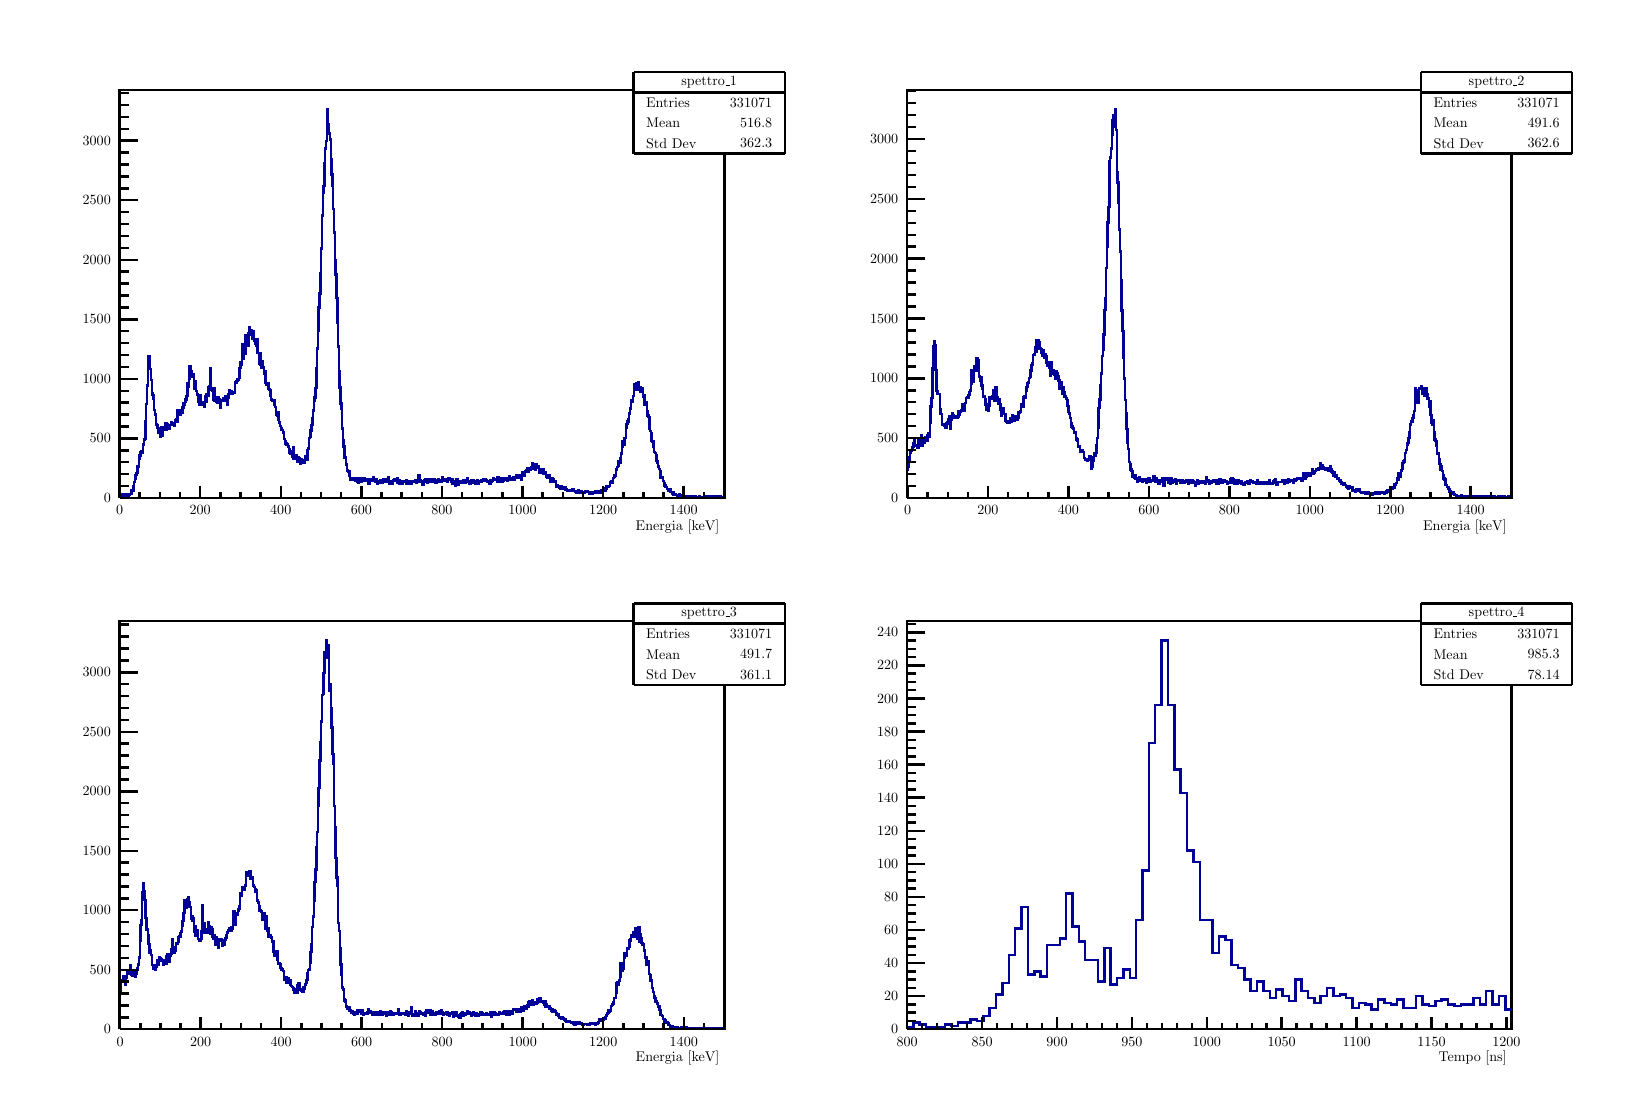
\begin{tikzpicture}
\pgfdeclareplotmark{cross} {
\pgfpathmoveto{\pgfpoint{-0.3\pgfplotmarksize}{\pgfplotmarksize}}
\pgfpathlineto{\pgfpoint{+0.3\pgfplotmarksize}{\pgfplotmarksize}}
\pgfpathlineto{\pgfpoint{+0.3\pgfplotmarksize}{0.3\pgfplotmarksize}}
\pgfpathlineto{\pgfpoint{+1\pgfplotmarksize}{0.3\pgfplotmarksize}}
\pgfpathlineto{\pgfpoint{+1\pgfplotmarksize}{-0.3\pgfplotmarksize}}
\pgfpathlineto{\pgfpoint{+0.3\pgfplotmarksize}{-0.3\pgfplotmarksize}}
\pgfpathlineto{\pgfpoint{+0.3\pgfplotmarksize}{-1.\pgfplotmarksize}}
\pgfpathlineto{\pgfpoint{-0.3\pgfplotmarksize}{-1.\pgfplotmarksize}}
\pgfpathlineto{\pgfpoint{-0.3\pgfplotmarksize}{-0.3\pgfplotmarksize}}
\pgfpathlineto{\pgfpoint{-1.\pgfplotmarksize}{-0.3\pgfplotmarksize}}
\pgfpathlineto{\pgfpoint{-1.\pgfplotmarksize}{0.3\pgfplotmarksize}}
\pgfpathlineto{\pgfpoint{-0.3\pgfplotmarksize}{0.3\pgfplotmarksize}}
\pgfpathclose
\pgfusepathqstroke
}
\pgfdeclareplotmark{cross*} {
\pgfpathmoveto{\pgfpoint{-0.3\pgfplotmarksize}{\pgfplotmarksize}}
\pgfpathlineto{\pgfpoint{+0.3\pgfplotmarksize}{\pgfplotmarksize}}
\pgfpathlineto{\pgfpoint{+0.3\pgfplotmarksize}{0.3\pgfplotmarksize}}
\pgfpathlineto{\pgfpoint{+1\pgfplotmarksize}{0.3\pgfplotmarksize}}
\pgfpathlineto{\pgfpoint{+1\pgfplotmarksize}{-0.3\pgfplotmarksize}}
\pgfpathlineto{\pgfpoint{+0.3\pgfplotmarksize}{-0.3\pgfplotmarksize}}
\pgfpathlineto{\pgfpoint{+0.3\pgfplotmarksize}{-1.\pgfplotmarksize}}
\pgfpathlineto{\pgfpoint{-0.3\pgfplotmarksize}{-1.\pgfplotmarksize}}
\pgfpathlineto{\pgfpoint{-0.3\pgfplotmarksize}{-0.3\pgfplotmarksize}}
\pgfpathlineto{\pgfpoint{-1.\pgfplotmarksize}{-0.3\pgfplotmarksize}}
\pgfpathlineto{\pgfpoint{-1.\pgfplotmarksize}{0.3\pgfplotmarksize}}
\pgfpathlineto{\pgfpoint{-0.3\pgfplotmarksize}{0.3\pgfplotmarksize}}
\pgfpathclose
\pgfusepathqfillstroke
}
\pgfdeclareplotmark{newstar} {
\pgfpathmoveto{\pgfqpoint{0pt}{\pgfplotmarksize}}
\pgfpathlineto{\pgfqpointpolar{44}{0.5\pgfplotmarksize}}
\pgfpathlineto{\pgfqpointpolar{18}{\pgfplotmarksize}}
\pgfpathlineto{\pgfqpointpolar{-20}{0.5\pgfplotmarksize}}
\pgfpathlineto{\pgfqpointpolar{-54}{\pgfplotmarksize}}
\pgfpathlineto{\pgfqpointpolar{-90}{0.5\pgfplotmarksize}}
\pgfpathlineto{\pgfqpointpolar{234}{\pgfplotmarksize}}
\pgfpathlineto{\pgfqpointpolar{198}{0.5\pgfplotmarksize}}
\pgfpathlineto{\pgfqpointpolar{162}{\pgfplotmarksize}}
\pgfpathlineto{\pgfqpointpolar{134}{0.5\pgfplotmarksize}}
\pgfpathclose
\pgfusepathqstroke
}
\pgfdeclareplotmark{newstar*} {
\pgfpathmoveto{\pgfqpoint{0pt}{\pgfplotmarksize}}
\pgfpathlineto{\pgfqpointpolar{44}{0.5\pgfplotmarksize}}
\pgfpathlineto{\pgfqpointpolar{18}{\pgfplotmarksize}}
\pgfpathlineto{\pgfqpointpolar{-20}{0.5\pgfplotmarksize}}
\pgfpathlineto{\pgfqpointpolar{-54}{\pgfplotmarksize}}
\pgfpathlineto{\pgfqpointpolar{-90}{0.5\pgfplotmarksize}}
\pgfpathlineto{\pgfqpointpolar{234}{\pgfplotmarksize}}
\pgfpathlineto{\pgfqpointpolar{198}{0.5\pgfplotmarksize}}
\pgfpathlineto{\pgfqpointpolar{162}{\pgfplotmarksize}}
\pgfpathlineto{\pgfqpointpolar{134}{0.5\pgfplotmarksize}}
\pgfpathclose
\pgfusepathqfillstroke
}
\definecolor{c}{rgb}{1,1,1};
\draw [color=c, fill=c] (0,0) rectangle (20,13.4957);
\draw [color=c, fill=c] (0.2,6.88281) rectangle (9.8,13.3607);
\draw [color=c, fill=c] (1.16,7.5306) rectangle (8.84,12.713);
\definecolor{c}{rgb}{0,0,0};
\draw [c,line width=0.9] (1.16,7.5306) -- (1.16,12.713) -- (8.84,12.713) -- (8.84,7.5306) -- (1.16,7.5306);
\definecolor{c}{rgb}{1,1,1};
\draw [color=c, fill=c] (1.16,7.5306) rectangle (8.84,12.713);
\definecolor{c}{rgb}{0,0,0};
\draw [c,line width=0.9] (1.16,7.5306) -- (1.16,12.713) -- (8.84,12.713) -- (8.84,7.5306) -- (1.16,7.5306);
\definecolor{c}{rgb}{0,0,0.6};
\draw [c,line width=0.9] (1.16,7.57748) -- (1.17024,7.57748) -- (1.17024,7.57445) -- (1.18048,7.57445) -- (1.18048,7.56387) -- (1.19072,7.56387) -- (1.19072,7.57294) -- (1.20096,7.57294) -- (1.20096,7.5805) -- (1.2112,7.5805) -- (1.2112,7.56538) --
 (1.22144,7.56538) -- (1.22144,7.5548) -- (1.23168,7.5548) -- (1.23168,7.56236) -- (1.24192,7.56236) -- (1.24192,7.57294) -- (1.25216,7.57294) -- (1.25216,7.57445) -- (1.2624,7.57445) -- (1.2624,7.56236) -- (1.27264,7.56236) -- (1.27264,7.57748) --
 (1.28288,7.57748) -- (1.28288,7.5684) -- (1.29312,7.5684) -- (1.29312,7.57899) -- (1.30336,7.57899) -- (1.30336,7.58806) -- (1.3136,7.58806) -- (1.3136,7.62435) -- (1.32384,7.62435) -- (1.32384,7.62738) -- (1.33408,7.62738) -- (1.33408,7.6803) --
 (1.34432,7.6803) -- (1.34432,7.73474) -- (1.35456,7.73474) -- (1.35456,7.77557) -- (1.3648,7.77557) -- (1.3648,7.81942) -- (1.37504,7.81942) -- (1.37504,7.84966) -- (1.38528,7.84966) -- (1.38528,7.92829) -- (1.39552,7.92829) -- (1.39552,7.92829) --
 (1.40576,7.92829) -- (1.40576,8.03263) -- (1.416,8.03263) -- (1.416,8.07043) -- (1.42624,8.07043) -- (1.42624,8.10823) -- (1.43648,8.10823) -- (1.43648,8.1294) -- (1.44672,8.1294) -- (1.44672,8.10672) -- (1.45696,8.10672) -- (1.45696,8.21106) --
 (1.4672,8.21106) -- (1.4672,8.26549) -- (1.47744,8.26549) -- (1.47744,8.28061) -- (1.48768,8.28061) -- (1.48768,8.50895) -- (1.49792,8.50895) -- (1.49792,8.72367) -- (1.50816,8.72367) -- (1.50816,8.96107) -- (1.5184,8.96107) -- (1.5184,9.23628) --
 (1.52864,9.23628) -- (1.52864,9.32398) -- (1.53888,9.32398) -- (1.53888,9.3134) -- (1.54912,9.3134) -- (1.54912,9.16521) -- (1.55936,9.16521) -- (1.55936,9.0276) -- (1.5696,9.0276) -- (1.5696,8.85371) -- (1.57984,8.85371) -- (1.57984,8.83708) --
 (1.59008,8.83708) -- (1.59008,8.78718) -- (1.60032,8.78718) -- (1.60032,8.64806) -- (1.61056,8.64806) -- (1.61056,8.59211) -- (1.6208,8.59211) -- (1.6208,8.47114) -- (1.63104,8.47114) -- (1.63104,8.45602) -- (1.64128,8.45602) -- (1.64128,8.41671) --
 (1.65152,8.41671) -- (1.65152,8.35773) -- (1.66176,8.35773) -- (1.66176,8.39856) -- (1.672,8.39856) -- (1.672,8.30935) -- (1.68224,8.30935) -- (1.68224,8.3411) -- (1.69248,8.3411) -- (1.69248,8.43032) -- (1.70272,8.43032) -- (1.70272,8.32144) --
 (1.71296,8.32144) -- (1.71296,8.40915) -- (1.7232,8.40915) -- (1.7232,8.41217) -- (1.73344,8.41217) -- (1.73344,8.40158) -- (1.74368,8.40158) -- (1.74368,8.48173) -- (1.75392,8.48173) -- (1.75392,8.40007) -- (1.76416,8.40007) -- (1.76416,8.46963) --
 (1.7744,8.46963) -- (1.7744,8.45148) -- (1.78464,8.45148) -- (1.78464,8.41066) -- (1.79488,8.41066) -- (1.79488,8.45451) -- (1.80512,8.45451) -- (1.80512,8.45602) -- (1.81536,8.45602) -- (1.81536,8.48929) -- (1.8256,8.48929) -- (1.8256,8.47719) --
 (1.83584,8.47719) -- (1.83584,8.45451) -- (1.84608,8.45451) -- (1.84608,8.45753) -- (1.85632,8.45753) -- (1.85632,8.4409) -- (1.86656,8.4409) -- (1.86656,8.51802) -- (1.8768,8.51802) -- (1.8768,8.53012) -- (1.88704,8.53012) -- (1.88704,8.49836) --
 (1.89728,8.49836) -- (1.89728,8.64352) -- (1.90752,8.64352) -- (1.90752,8.58153) -- (1.91776,8.58153) -- (1.91776,8.58304) -- (1.928,8.58304) -- (1.928,8.58909) -- (1.93824,8.58909) -- (1.93824,8.64957) -- (1.94848,8.64957) -- (1.94848,8.61782) --
 (1.95872,8.61782) -- (1.95872,8.68133) -- (1.96896,8.68133) -- (1.96896,8.73123) -- (1.9792,8.73123) -- (1.9792,8.71611) -- (1.98944,8.71611) -- (1.98944,8.74937) -- (1.99968,8.74937) -- (1.99968,8.7781) -- (2.00992,8.7781) -- (2.00992,8.82195) --
 (2.02016,8.82195) -- (2.02016,8.98375) -- (2.0304,8.98375) -- (2.0304,8.94292) -- (2.04064,8.94292) -- (2.04064,9.04424) -- (2.05088,9.04424) -- (2.05088,9.19696) -- (2.06112,9.19696) -- (2.06112,9.14555) -- (2.07136,9.14555) -- (2.07136,9.08658) --
 (2.0816,9.08658) -- (2.0816,9.06994) -- (2.09184,9.06994) -- (2.09184,9.09867) -- (2.10208,9.09867) -- (2.10208,8.91571) -- (2.11232,8.91571) -- (2.11232,9.00795) -- (2.12256,9.00795) -- (2.12256,8.92932) -- (2.1328,8.92932) -- (2.1328,8.89151) --
 (2.14304,8.89151) -- (2.14304,8.84615) -- (2.15328,8.84615) -- (2.15328,8.83103) -- (2.16352,8.83103) -- (2.16352,8.74937) -- (2.17376,8.74937) -- (2.17376,8.71762) -- (2.184,8.71762) -- (2.184,8.83254) -- (2.19424,8.83254) -- (2.19424,8.72972) --
 (2.20448,8.72972) -- (2.20448,8.71308) -- (2.21472,8.71308) -- (2.21472,8.74332) -- (2.22496,8.74332) -- (2.22496,8.74332) -- (2.2352,8.74332) -- (2.2352,8.6904) -- (2.24544,8.6904) -- (2.24544,8.82195) -- (2.25568,8.82195) -- (2.25568,8.75391) --
 (2.26592,8.75391) -- (2.26592,8.84464) -- (2.27616,8.84464) -- (2.27616,8.83254) -- (2.2864,8.83254) -- (2.2864,8.93234) -- (2.29664,8.93234) -- (2.29664,8.95049) -- (2.30688,8.95049) -- (2.30688,9.1773) -- (2.31712,9.1773) -- (2.31712,8.90663) --
 (2.32736,8.90663) -- (2.32736,8.92478) -- (2.3376,8.92478) -- (2.3376,8.89756) -- (2.34784,8.89756) -- (2.34784,8.78264) -- (2.35808,8.78264) -- (2.35808,8.92175) -- (2.36832,8.92175) -- (2.36832,8.75996) -- (2.37856,8.75996) -- (2.37856,8.80683) --
 (2.3888,8.80683) -- (2.3888,8.74937) -- (2.39904,8.74937) -- (2.39904,8.73425) -- (2.40928,8.73425) -- (2.40928,8.81288) -- (2.41952,8.81288) -- (2.41952,8.78113) -- (2.42976,8.78113) -- (2.42976,8.75996) -- (2.44,8.75996) -- (2.44,8.67528) --
 (2.45024,8.67528) -- (2.45024,8.77054) -- (2.46048,8.77054) -- (2.46048,8.76903) -- (2.47072,8.76903) -- (2.47072,8.80079) -- (2.48096,8.80079) -- (2.48096,8.77357) -- (2.4912,8.77357) -- (2.4912,8.76601) -- (2.50144,8.76601) -- (2.50144,8.82195) --
 (2.51168,8.82195) -- (2.51168,8.80683) -- (2.52192,8.80683) -- (2.52192,8.71459) -- (2.53216,8.71459) -- (2.53216,8.80683) -- (2.5424,8.80683) -- (2.5424,8.84766) -- (2.55264,8.84766) -- (2.55264,8.90059) -- (2.56288,8.90059) -- (2.56288,8.87488) --
 (2.57312,8.87488) -- (2.57312,8.89) -- (2.58336,8.89) -- (2.58336,8.85069) -- (2.5936,8.85069) -- (2.5936,8.86429) -- (2.60384,8.86429) -- (2.60384,8.87639) -- (2.61408,8.87639) -- (2.61408,8.86732) -- (2.62432,8.86732) -- (2.62432,9.0019) --
 (2.63456,9.0019) -- (2.63456,8.98829) -- (2.6448,8.98829) -- (2.6448,9.014) -- (2.65504,9.014) -- (2.65504,9.04121) -- (2.66528,9.04121) -- (2.66528,9.03214) -- (2.67552,9.03214) -- (2.67552,9.05029) -- (2.68576,9.05029) -- (2.68576,9.1773) --
 (2.696,9.1773) -- (2.696,9.24989) -- (2.70624,9.24989) -- (2.70624,9.22418) -- (2.71648,9.22418) -- (2.71648,9.4767) -- (2.72672,9.4767) -- (2.72672,9.29827) -- (2.73696,9.29827) -- (2.73696,9.38447) -- (2.7472,9.38447) -- (2.7472,9.35725) --
 (2.75744,9.35725) -- (2.75744,9.59163) -- (2.76768,9.59163) -- (2.76768,9.53719) -- (2.77792,9.53719) -- (2.77792,9.58709) -- (2.78816,9.58709) -- (2.78816,9.46612) -- (2.7984,9.46612) -- (2.7984,9.62792) -- (2.80864,9.62792) -- (2.80864,9.69294) --
 (2.81888,9.69294) -- (2.81888,9.6007) -- (2.82912,9.6007) -- (2.82912,9.66118) -- (2.83936,9.66118) -- (2.83936,9.54626) -- (2.8496,9.54626) -- (2.8496,9.6506) -- (2.85984,9.6506) -- (2.85984,9.62036) -- (2.87008,9.62036) -- (2.87008,9.52963) --
 (2.88032,9.52963) -- (2.88032,9.48427) -- (2.89056,9.48427) -- (2.89056,9.46914) -- (2.9008,9.46914) -- (2.9008,9.54173) -- (2.91104,9.54173) -- (2.91104,9.36783) -- (2.92128,9.36783) -- (2.92128,9.36934) -- (2.93152,9.36934) -- (2.93152,9.23174) --
 (2.94176,9.23174) -- (2.94176,9.3633) -- (2.952,9.3633) -- (2.952,9.22116) -- (2.96224,9.22116) -- (2.96224,9.18638) -- (2.97248,9.18638) -- (2.97248,9.26652) -- (2.98272,9.26652) -- (2.98272,9.19243) -- (2.99296,9.19243) -- (2.99296,9.10321) --
 (3.0032,9.10321) -- (3.0032,9.13799) -- (3.01344,9.13799) -- (3.01344,8.99282) -- (3.02368,8.99282) -- (3.02368,8.97014) -- (3.03392,8.97014) -- (3.03392,8.97922) -- (3.04416,8.97922) -- (3.04416,8.99131) -- (3.0544,8.99131) -- (3.0544,8.91571) --
 (3.06464,8.91571) -- (3.06464,8.9021) -- (3.07488,8.9021) -- (3.07488,8.83405) -- (3.08512,8.83405) -- (3.08512,8.78113) -- (3.09536,8.78113) -- (3.09536,8.76298) -- (3.1056,8.76298) -- (3.1056,8.76449) -- (3.11584,8.76449) -- (3.11584,8.77054) --
 (3.12608,8.77054) -- (3.12608,8.71157) -- (3.13632,8.71157) -- (3.13632,8.68435) -- (3.14656,8.68435) -- (3.14656,8.58909) -- (3.1568,8.58909) -- (3.1568,8.57548) -- (3.16704,8.57548) -- (3.16704,8.62387) -- (3.17728,8.62387) -- (3.17728,8.52407) --
 (3.18752,8.52407) -- (3.18752,8.48929) -- (3.19776,8.48929) -- (3.19776,8.4409) -- (3.208,8.4409) -- (3.208,8.41519) -- (3.21824,8.41519) -- (3.21824,8.39554) -- (3.22848,8.39554) -- (3.22848,8.39251) -- (3.23872,8.39251) -- (3.23872,8.36076) --
 (3.24896,8.36076) -- (3.24896,8.28061) -- (3.2592,8.28061) -- (3.2592,8.24735) -- (3.26944,8.24735) -- (3.26944,8.21862) -- (3.27968,8.21862) -- (3.27968,8.21106) -- (3.28992,8.21106) -- (3.28992,8.21711) -- (3.30016,8.21711) -- (3.30016,8.18384) --
 (3.3104,8.18384) -- (3.3104,8.15057) -- (3.32064,8.15057) -- (3.32064,8.1037) -- (3.33088,8.1037) -- (3.33088,8.08555) -- (3.34112,8.08555) -- (3.34112,8.12789) -- (3.35136,8.12789) -- (3.35136,8.05077) -- (3.3616,8.05077) -- (3.3616,8.17477) --
 (3.37184,8.17477) -- (3.37184,8.03414) -- (3.38208,8.03414) -- (3.38208,8.04321) -- (3.39232,8.04321) -- (3.39232,8.02507) -- (3.40256,8.02507) -- (3.40256,8.06741) -- (3.4128,8.06741) -- (3.4128,7.98726) -- (3.42304,7.98726) -- (3.42304,8.04624) --
 (3.43328,8.04624) -- (3.43328,7.98878) -- (3.44352,7.98878) -- (3.44352,8.02809) -- (3.45376,8.02809) -- (3.45376,7.95853) -- (3.464,7.95853) -- (3.464,8.02053) -- (3.47424,8.02053) -- (3.47424,7.97365) -- (3.48448,7.97365) -- (3.48448,7.9797) --
 (3.49472,7.9797) -- (3.49472,8.00843) -- (3.50496,8.00843) -- (3.50496,7.97668) -- (3.5152,7.97668) -- (3.5152,8.05682) -- (3.52544,8.05682) -- (3.52544,8.02204) -- (3.53568,8.02204) -- (3.53568,8.01448) -- (3.54592,8.01448) -- (3.54592,8.13091) --
 (3.55616,8.13091) -- (3.55616,8.15662) -- (3.5664,8.15662) -- (3.5664,8.29271) -- (3.57664,8.29271) -- (3.57664,8.30481) -- (3.58688,8.30481) -- (3.58688,8.38646) -- (3.59712,8.38646) -- (3.59712,8.45602) -- (3.60736,8.45602) -- (3.60736,8.53919) --
 (3.6176,8.53919) -- (3.6176,8.6405) -- (3.62784,8.6405) -- (3.62784,8.76601) -- (3.63808,8.76601) -- (3.63808,8.80683) -- (3.64832,8.80683) -- (3.64832,8.92327) -- (3.65856,8.92327) -- (3.65856,9.17579) -- (3.6688,9.17579) -- (3.6688,9.42983) --
 (3.67904,9.42983) -- (3.67904,9.64757) -- (3.68928,9.64757) -- (3.68928,9.94849) -- (3.69952,9.94849) -- (3.69952,10.1239) -- (3.70976,10.1239) -- (3.70976,10.384) -- (3.72,10.384) -- (3.72,10.6955) -- (3.73024,10.6955) -- (3.73024,11.1174) --
 (3.74048,11.1174) -- (3.74048,11.4062) -- (3.75072,11.4062) -- (3.75072,11.4939) -- (3.76096,11.4939) -- (3.76096,11.7857) -- (3.7712,11.7857) -- (3.7712,11.9672) -- (3.78144,11.9672) -- (3.78144,12.0609) -- (3.79168,12.0609) -- (3.79168,12.4662) --
 (3.80192,12.4662) -- (3.80192,12.1607) -- (3.81216,12.1607) -- (3.81216,12.2772) -- (3.8224,12.2772) -- (3.8224,12.1668) -- (3.83264,12.1668) -- (3.83264,12.0821) -- (3.84288,12.0821) -- (3.84288,11.8371) -- (3.85312,11.8371) -- (3.85312,11.6406) --
 (3.86336,11.6406) -- (3.86336,11.4954) -- (3.8736,11.4954) -- (3.8736,11.2005) -- (3.88384,11.2005) -- (3.88384,10.9011) -- (3.89408,10.9011) -- (3.89408,10.5548) -- (3.90432,10.5548) -- (3.90432,10.3673) -- (3.91456,10.3673) -- (3.91456,10.0664) --
 (3.9248,10.0664) -- (3.9248,9.75796) -- (3.93504,9.75796) -- (3.93504,9.45251) -- (3.94528,9.45251) -- (3.94528,9.13496) -- (3.95552,9.13496) -- (3.95552,8.93536) -- (3.96576,8.93536) -- (3.96576,8.72669) -- (3.976,8.72669) -- (3.976,8.65713) --
 (3.98624,8.65713) -- (3.98624,8.40915) -- (3.99648,8.40915) -- (3.99648,8.26701) -- (4.00672,8.26701) -- (4.00672,8.18081) -- (4.01696,8.18081) -- (4.01696,8.04321) -- (4.0272,8.04321) -- (4.0272,8.03868) -- (4.03744,8.03868) -- (4.03744,7.954) --
 (4.04768,7.954) -- (4.04768,7.88141) -- (4.05792,7.88141) -- (4.05792,7.86932) -- (4.06816,7.86932) -- (4.06816,7.86478) -- (4.0784,7.86478) -- (4.0784,7.81337) -- (4.08864,7.81337) -- (4.08864,7.76649) -- (4.09888,7.76649) -- (4.09888,7.78161) --
 (4.10912,7.78161) -- (4.10912,7.75893) -- (4.11936,7.75893) -- (4.11936,7.7801) -- (4.1296,7.7801) -- (4.1296,7.76649) -- (4.13984,7.76649) -- (4.13984,7.78615) -- (4.15008,7.78615) -- (4.15008,7.74532) -- (4.16032,7.74532) -- (4.16032,7.77557) --
 (4.17056,7.77557) -- (4.17056,7.76044) -- (4.1808,7.76044) -- (4.1808,7.73927) -- (4.19104,7.73927) -- (4.19104,7.72718) -- (4.20128,7.72718) -- (4.20128,7.77405) -- (4.21152,7.77405) -- (4.21152,7.7544) -- (4.22176,7.7544) -- (4.22176,7.74079) --
 (4.232,7.74079) -- (4.232,7.76498) -- (4.24224,7.76498) -- (4.24224,7.78464) -- (4.25248,7.78464) -- (4.25248,7.74986) -- (4.26272,7.74986) -- (4.26272,7.77859) -- (4.27296,7.77859) -- (4.27296,7.74532) -- (4.2832,7.74532) -- (4.2832,7.76196) --
 (4.29344,7.76196) -- (4.29344,7.74835) -- (4.30368,7.74835) -- (4.30368,7.76347) -- (4.31392,7.76347) -- (4.31392,7.77254) -- (4.32416,7.77254) -- (4.32416,7.71508) -- (4.3344,7.71508) -- (4.3344,7.76196) -- (4.34464,7.76196) -- (4.34464,7.74835) --
 (4.35488,7.74835) -- (4.35488,7.7544) -- (4.36512,7.7544) -- (4.36512,7.74532) -- (4.37536,7.74532) -- (4.37536,7.78766) -- (4.3856,7.78766) -- (4.3856,7.75137) -- (4.39584,7.75137) -- (4.39584,7.76196) -- (4.40608,7.76196) -- (4.40608,7.7302) --
 (4.41632,7.7302) -- (4.41632,7.76498) -- (4.42656,7.76498) -- (4.42656,7.71659) -- (4.4368,7.71659) -- (4.4368,7.73171) -- (4.44704,7.73171) -- (4.44704,7.74381) -- (4.45728,7.74381) -- (4.45728,7.72718) -- (4.46752,7.72718) -- (4.46752,7.75288) --
 (4.47776,7.75288) -- (4.47776,7.75591) -- (4.488,7.75591) -- (4.488,7.73927) -- (4.49824,7.73927) -- (4.49824,7.72718) -- (4.50848,7.72718) -- (4.50848,7.76347) -- (4.51872,7.76347) -- (4.51872,7.76347) -- (4.52896,7.76347) -- (4.52896,7.76347) --
 (4.5392,7.76347) -- (4.5392,7.73927) -- (4.54944,7.73927) -- (4.54944,7.73625) -- (4.55968,7.73625) -- (4.55968,7.74986) -- (4.56992,7.74986) -- (4.56992,7.78766) -- (4.58016,7.78766) -- (4.58016,7.71357) -- (4.5904,7.71357) -- (4.5904,7.72567) --
 (4.60064,7.72567) -- (4.60064,7.74381) -- (4.61088,7.74381) -- (4.61088,7.74381) -- (4.62112,7.74381) -- (4.62112,7.71659) -- (4.63136,7.71659) -- (4.63136,7.76044) -- (4.6416,7.76044) -- (4.6416,7.75742) -- (4.65184,7.75742) -- (4.65184,7.768) --
 (4.66208,7.768) -- (4.66208,7.7423) -- (4.67232,7.7423) -- (4.67232,7.76649) -- (4.68256,7.76649) -- (4.68256,7.77557) -- (4.6928,7.77557) -- (4.6928,7.72567) -- (4.70304,7.72567) -- (4.70304,7.7544) -- (4.71328,7.7544) -- (4.71328,7.71659) --
 (4.72352,7.71659) -- (4.72352,7.73625) -- (4.73376,7.73625) -- (4.73376,7.73625) -- (4.744,7.73625) -- (4.744,7.70903) -- (4.75424,7.70903) -- (4.75424,7.74835) -- (4.76448,7.74835) -- (4.76448,7.73625) -- (4.77472,7.73625) -- (4.77472,7.73323) --
 (4.78496,7.73323) -- (4.78496,7.73625) -- (4.7952,7.73625) -- (4.7952,7.7544) -- (4.80544,7.7544) -- (4.80544,7.71508) -- (4.81568,7.71508) -- (4.81568,7.74684) -- (4.82592,7.74684) -- (4.82592,7.73927) -- (4.83616,7.73927) -- (4.83616,7.74684) --
 (4.8464,7.74684) -- (4.8464,7.72113) -- (4.85664,7.72113) -- (4.85664,7.70752) -- (4.86688,7.70752) -- (4.86688,7.7302) -- (4.87712,7.7302) -- (4.87712,7.73625) -- (4.88736,7.73625) -- (4.88736,7.74532) -- (4.8976,7.74532) -- (4.8976,7.73625) --
 (4.90784,7.73625) -- (4.90784,7.73474) -- (4.91808,7.73474) -- (4.91808,7.7544) -- (4.92832,7.7544) -- (4.92832,7.7181) -- (4.93856,7.7181) -- (4.93856,7.73171) -- (4.9488,7.73171) -- (4.9488,7.73927) -- (4.95904,7.73927) -- (4.95904,7.81488) --
 (4.96928,7.81488) -- (4.96928,7.75742) -- (4.97952,7.75742) -- (4.97952,7.74532) -- (4.98976,7.74532) -- (4.98976,7.7302) -- (5,7.7302) -- (5,7.74835) -- (5.01024,7.74835) -- (5.01024,7.69542) -- (5.02048,7.69542) -- (5.02048,7.73776) --
 (5.03072,7.73776) -- (5.03072,7.75137) -- (5.04096,7.75137) -- (5.04096,7.76498) -- (5.0512,7.76498) -- (5.0512,7.76196) -- (5.06144,7.76196) -- (5.06144,7.72415) -- (5.07168,7.72415) -- (5.07168,7.76347) -- (5.08192,7.76347) -- (5.08192,7.75742) --
 (5.09216,7.75742) -- (5.09216,7.73927) -- (5.1024,7.73927) -- (5.1024,7.7544) -- (5.11264,7.7544) -- (5.11264,7.76347) -- (5.12288,7.76347) -- (5.12288,7.73171) -- (5.13312,7.73171) -- (5.13312,7.75591) -- (5.14336,7.75591) -- (5.14336,7.75137) --
 (5.1536,7.75137) -- (5.1536,7.768) -- (5.16384,7.768) -- (5.16384,7.75591) -- (5.17408,7.75591) -- (5.17408,7.7181) -- (5.18432,7.7181) -- (5.18432,7.7544) -- (5.19456,7.7544) -- (5.19456,7.75137) -- (5.2048,7.75137) -- (5.2048,7.768) --
 (5.21504,7.768) -- (5.21504,7.75893) -- (5.22528,7.75893) -- (5.22528,7.73776) -- (5.23552,7.73776) -- (5.23552,7.74684) -- (5.24576,7.74684) -- (5.24576,7.74079) -- (5.256,7.74079) -- (5.256,7.79825) -- (5.26624,7.79825) -- (5.26624,7.7544) --
 (5.27648,7.7544) -- (5.27648,7.75893) -- (5.28672,7.75893) -- (5.28672,7.76196) -- (5.29696,7.76196) -- (5.29696,7.74381) -- (5.3072,7.74381) -- (5.3072,7.74381) -- (5.31744,7.74381) -- (5.31744,7.74079) -- (5.32768,7.74079) -- (5.32768,7.76649) --
 (5.33792,7.76649) -- (5.33792,7.77859) -- (5.34816,7.77859) -- (5.34816,7.75893) -- (5.3584,7.75893) -- (5.3584,7.75591) -- (5.36864,7.75591) -- (5.36864,7.73171) -- (5.37888,7.73171) -- (5.37888,7.76952) -- (5.38912,7.76952) -- (5.38912,7.71659) --
 (5.39936,7.71659) -- (5.39936,7.73474) -- (5.4096,7.73474) -- (5.4096,7.74532) -- (5.41984,7.74532) -- (5.41984,7.69089) -- (5.43008,7.69089) -- (5.43008,7.74532) -- (5.44032,7.74532) -- (5.44032,7.77103) -- (5.45056,7.77103) -- (5.45056,7.76649) --
 (5.4608,7.76649) -- (5.4608,7.70298) -- (5.47104,7.70298) -- (5.47104,7.74381) -- (5.48128,7.74381) -- (5.48128,7.72869) -- (5.49152,7.72869) -- (5.49152,7.74684) -- (5.50176,7.74684) -- (5.50176,7.72415) -- (5.512,7.72415) -- (5.512,7.73625) --
 (5.52224,7.73625) -- (5.52224,7.75893) -- (5.53248,7.75893) -- (5.53248,7.72264) -- (5.54272,7.72264) -- (5.54272,7.72869) -- (5.55296,7.72869) -- (5.55296,7.74079) -- (5.5632,7.74079) -- (5.5632,7.7544) -- (5.57344,7.7544) -- (5.57344,7.77405) --
 (5.58368,7.77405) -- (5.58368,7.7302) -- (5.59392,7.7302) -- (5.59392,7.74835) -- (5.60416,7.74835) -- (5.60416,7.71508) -- (5.6144,7.71508) -- (5.6144,7.71508) -- (5.62464,7.71508) -- (5.62464,7.75288) -- (5.63488,7.75288) -- (5.63488,7.72567) --
 (5.64512,7.72567) -- (5.64512,7.74986) -- (5.65536,7.74986) -- (5.65536,7.74835) -- (5.6656,7.74835) -- (5.6656,7.73474) -- (5.67584,7.73474) -- (5.67584,7.71206) -- (5.68608,7.71206) -- (5.68608,7.74684) -- (5.69632,7.74684) -- (5.69632,7.75288) --
 (5.70656,7.75288) -- (5.70656,7.70903) -- (5.7168,7.70903) -- (5.7168,7.7423) -- (5.72704,7.7423) -- (5.72704,7.73323) -- (5.73728,7.73323) -- (5.73728,7.7302) -- (5.74752,7.7302) -- (5.74752,7.73927) -- (5.75776,7.73927) -- (5.75776,7.75591) --
 (5.768,7.75591) -- (5.768,7.75137) -- (5.77824,7.75137) -- (5.77824,7.76196) -- (5.78848,7.76196) -- (5.78848,7.75137) -- (5.79872,7.75137) -- (5.79872,7.76196) -- (5.80896,7.76196) -- (5.80896,7.75893) -- (5.8192,7.75893) -- (5.8192,7.74986) --
 (5.82944,7.74986) -- (5.82944,7.73776) -- (5.83968,7.73776) -- (5.83968,7.73625) -- (5.84992,7.73625) -- (5.84992,7.73625) -- (5.86016,7.73625) -- (5.86016,7.71508) -- (5.8704,7.71508) -- (5.8704,7.75288) -- (5.88064,7.75288) -- (5.88064,7.73927) --
 (5.89088,7.73927) -- (5.89088,7.74986) -- (5.90112,7.74986) -- (5.90112,7.78161) -- (5.91136,7.78161) -- (5.91136,7.76044) -- (5.9216,7.76044) -- (5.9216,7.76044) -- (5.93184,7.76044) -- (5.93184,7.76649) -- (5.94208,7.76649) -- (5.94208,7.76498) --
 (5.95232,7.76498) -- (5.95232,7.74079) -- (5.96256,7.74079) -- (5.96256,7.78766) -- (5.9728,7.78766) -- (5.9728,7.73323) -- (5.98304,7.73323) -- (5.98304,7.74684) -- (5.99328,7.74684) -- (5.99328,7.768) -- (6.00352,7.768) -- (6.00352,7.77708) --
 (6.01376,7.77708) -- (6.01376,7.73171) -- (6.024,7.73171) -- (6.024,7.75591) -- (6.03424,7.75591) -- (6.03424,7.74684) -- (6.04448,7.74684) -- (6.04448,7.77859) -- (6.05472,7.77859) -- (6.05472,7.77557) -- (6.06496,7.77557) -- (6.06496,7.78615) --
 (6.0752,7.78615) -- (6.0752,7.76347) -- (6.08544,7.76347) -- (6.08544,7.7423) -- (6.09568,7.7423) -- (6.09568,7.75742) -- (6.10592,7.75742) -- (6.10592,7.80127) -- (6.11616,7.80127) -- (6.11616,7.76498) -- (6.1264,7.76498) -- (6.1264,7.76347) --
 (6.13664,7.76347) -- (6.13664,7.76044) -- (6.14688,7.76044) -- (6.14688,7.77557) -- (6.15712,7.77557) -- (6.15712,7.79069) -- (6.16736,7.79069) -- (6.16736,7.76347) -- (6.1776,7.76347) -- (6.1776,7.79522) -- (6.18784,7.79522) -- (6.18784,7.78464) --
 (6.19808,7.78464) -- (6.19808,7.82395) -- (6.20832,7.82395) -- (6.20832,7.79371) -- (6.21856,7.79371) -- (6.21856,7.81639) -- (6.2288,7.81639) -- (6.2288,7.78313) -- (6.23904,7.78313) -- (6.23904,7.81034) -- (6.24928,7.81034) -- (6.24928,7.8179) --
 (6.25952,7.8179) -- (6.25952,7.76498) -- (6.26976,7.76498) -- (6.26976,7.85117) -- (6.28,7.85117) -- (6.28,7.84361) -- (6.29024,7.84361) -- (6.29024,7.81034) -- (6.30048,7.81034) -- (6.30048,7.84966) -- (6.31072,7.84966) -- (6.31072,7.87537) --
 (6.32096,7.87537) -- (6.32096,7.87839) -- (6.3312,7.87839) -- (6.3312,7.90258) -- (6.34144,7.90258) -- (6.34144,7.86024) -- (6.35168,7.86024) -- (6.35168,7.87537) -- (6.36192,7.87537) -- (6.36192,7.91166) -- (6.37216,7.91166) -- (6.37216,7.89351) --
 (6.3824,7.89351) -- (6.3824,7.91771) -- (6.39264,7.91771) -- (6.39264,7.9041) -- (6.40288,7.9041) -- (6.40288,7.96458) -- (6.41312,7.96458) -- (6.41312,7.90107) -- (6.42336,7.90107) -- (6.42336,7.90561) -- (6.4336,7.90561) -- (6.4336,7.88444) --
 (6.44384,7.88444) -- (6.44384,7.96004) -- (6.45408,7.96004) -- (6.45408,7.92375) -- (6.46432,7.92375) -- (6.46432,7.91468) -- (6.47456,7.91468) -- (6.47456,7.92678) -- (6.4848,7.92678) -- (6.4848,7.89049) -- (6.49504,7.89049) -- (6.49504,7.85571) --
 (6.50528,7.85571) -- (6.50528,7.87688) -- (6.51552,7.87688) -- (6.51552,7.89956) -- (6.52576,7.89956) -- (6.52576,7.87385) -- (6.536,7.87385) -- (6.536,7.89502) -- (6.54624,7.89502) -- (6.54624,7.83454) -- (6.55648,7.83454) -- (6.55648,7.85268) --
 (6.56672,7.85268) -- (6.56672,7.86024) -- (6.57696,7.86024) -- (6.57696,7.8043) -- (6.5872,7.8043) -- (6.5872,7.78615) -- (6.59744,7.78615) -- (6.59744,7.81337) -- (6.60768,7.81337) -- (6.60768,7.79069) -- (6.61792,7.79069) -- (6.61792,7.81488) --
 (6.62816,7.81488) -- (6.62816,7.73776) -- (6.6384,7.73776) -- (6.6384,7.76649) -- (6.64864,7.76649) -- (6.64864,7.78313) -- (6.65888,7.78313) -- (6.65888,7.77254) -- (6.66912,7.77254) -- (6.66912,7.74079) -- (6.67936,7.74079) -- (6.67936,7.73171) --
 (6.6896,7.73171) -- (6.6896,7.7423) -- (6.69984,7.7423) -- (6.69984,7.68181) -- (6.71008,7.68181) -- (6.71008,7.67728) -- (6.72032,7.67728) -- (6.72032,7.69391) -- (6.73056,7.69391) -- (6.73056,7.67274) -- (6.7408,7.67274) -- (6.7408,7.66064) --
 (6.75104,7.66064) -- (6.75104,7.68333) -- (6.76128,7.68333) -- (6.76128,7.65006) -- (6.77152,7.65006) -- (6.77152,7.67425) -- (6.78176,7.67425) -- (6.78176,7.65611) -- (6.792,7.65611) -- (6.792,7.64855) -- (6.80224,7.64855) -- (6.80224,7.6546) --
 (6.81248,7.6546) -- (6.81248,7.66518) -- (6.82272,7.66518) -- (6.82272,7.63947) -- (6.83296,7.63947) -- (6.83296,7.63494) -- (6.8432,7.63494) -- (6.8432,7.61982) -- (6.85344,7.61982) -- (6.85344,7.62889) -- (6.86368,7.62889) -- (6.86368,7.62587) --
 (6.87392,7.62587) -- (6.87392,7.6183) -- (6.88416,7.6183) -- (6.88416,7.62435) -- (6.8944,7.62435) -- (6.8944,7.62738) -- (6.90464,7.62738) -- (6.90464,7.62133) -- (6.91488,7.62133) -- (6.91488,7.64099) -- (6.92512,7.64099) -- (6.92512,7.61528) --
 (6.93536,7.61528) -- (6.93536,7.6183) -- (6.9456,7.6183) -- (6.9456,7.60772) -- (6.95584,7.60772) -- (6.95584,7.59714) -- (6.96608,7.59714) -- (6.96608,7.59109) -- (6.97632,7.59109) -- (6.97632,7.61982) -- (6.98656,7.61982) -- (6.98656,7.62889) --
 (6.9968,7.62889) -- (6.9968,7.60923) -- (7.00704,7.60923) -- (7.00704,7.60167) -- (7.01728,7.60167) -- (7.01728,7.61226) -- (7.02752,7.61226) -- (7.02752,7.60318) -- (7.03776,7.60318) -- (7.03776,7.60318) -- (7.048,7.60318) -- (7.048,7.59562) --
 (7.05824,7.59562) -- (7.05824,7.60016) -- (7.06848,7.60016) -- (7.06848,7.60923) -- (7.07872,7.60923) -- (7.07872,7.6047) -- (7.08896,7.6047) -- (7.08896,7.60318) -- (7.0992,7.60318) -- (7.0992,7.60923) -- (7.10944,7.60923) -- (7.10944,7.6047) --
 (7.11968,7.6047) -- (7.11968,7.58353) -- (7.12992,7.58353) -- (7.12992,7.6047) -- (7.14016,7.6047) -- (7.14016,7.59109) -- (7.1504,7.59109) -- (7.1504,7.5805) -- (7.16064,7.5805) -- (7.16064,7.58201) -- (7.17088,7.58201) -- (7.17088,7.60167) --
 (7.18112,7.60167) -- (7.18112,7.60772) -- (7.19136,7.60772) -- (7.19136,7.60016) -- (7.2016,7.60016) -- (7.2016,7.61226) -- (7.21184,7.61226) -- (7.21184,7.60167) -- (7.22208,7.60167) -- (7.22208,7.60772) -- (7.23232,7.60772) -- (7.23232,7.60318) --
 (7.24256,7.60318) -- (7.24256,7.60923) -- (7.2528,7.60923) -- (7.2528,7.60167) -- (7.26304,7.60167) -- (7.26304,7.59562) -- (7.27328,7.59562) -- (7.27328,7.61528) -- (7.28352,7.61528) -- (7.28352,7.62738) -- (7.29376,7.62738) -- (7.29376,7.61982) --
 (7.304,7.61982) -- (7.304,7.62738) -- (7.31424,7.62738) -- (7.31424,7.65006) -- (7.32448,7.65006) -- (7.32448,7.62435) -- (7.33472,7.62435) -- (7.33472,7.64855) -- (7.34496,7.64855) -- (7.34496,7.67577) -- (7.3552,7.67577) -- (7.3552,7.6682) --
 (7.36544,7.6682) -- (7.36544,7.67123) -- (7.37568,7.67123) -- (7.37568,7.6803) -- (7.38592,7.6803) -- (7.38592,7.7181) -- (7.39616,7.7181) -- (7.39616,7.72567) -- (7.4064,7.72567) -- (7.4064,7.73776) -- (7.41664,7.73776) -- (7.41664,7.72415) --
 (7.42688,7.72415) -- (7.42688,7.78464) -- (7.43712,7.78464) -- (7.43712,7.79674) -- (7.44736,7.79674) -- (7.44736,7.81337) -- (7.4576,7.81337) -- (7.4576,7.81639) -- (7.46784,7.81639) -- (7.46784,7.88897) -- (7.47808,7.88897) -- (7.47808,7.92224) --
 (7.48832,7.92224) -- (7.48832,7.94039) -- (7.49856,7.94039) -- (7.49856,7.99482) -- (7.5088,7.99482) -- (7.5088,7.97214) -- (7.51904,7.97214) -- (7.51904,8.03414) -- (7.52928,8.03414) -- (7.52928,8.0916) -- (7.53952,8.0916) -- (7.53952,8.18384) --
 (7.54976,8.18384) -- (7.54976,8.25188) -- (7.56,8.25188) -- (7.56,8.20803) -- (7.57024,8.20803) -- (7.57024,8.28213) -- (7.58048,8.28213) -- (7.58048,8.29271) -- (7.59072,8.29271) -- (7.59072,8.41973) -- (7.60096,8.41973) -- (7.60096,8.46661) --
 (7.6112,8.46661) -- (7.6112,8.5029) -- (7.62144,8.5029) -- (7.62144,8.52407) -- (7.63168,8.52407) -- (7.63168,8.59967) -- (7.64192,8.59967) -- (7.64192,8.66621) -- (7.65216,8.66621) -- (7.65216,8.77357) -- (7.6624,8.77357) -- (7.6624,8.76752) --
 (7.67264,8.76752) -- (7.67264,8.75391) -- (7.68288,8.75391) -- (7.68288,8.82195) -- (7.69312,8.82195) -- (7.69312,8.97468) -- (7.70336,8.97468) -- (7.70336,8.94746) -- (7.7136,8.94746) -- (7.7136,8.90815) -- (7.72384,8.90815) -- (7.72384,8.98678) --
 (7.73408,8.98678) -- (7.73408,8.93688) -- (7.74432,8.93688) -- (7.74432,8.99585) -- (7.75456,8.99585) -- (7.75456,8.90361) -- (7.7648,8.90361) -- (7.7648,8.9399) -- (7.77504,8.9399) -- (7.77504,8.88093) -- (7.78528,8.88093) -- (7.78528,8.90966) --
 (7.79552,8.90966) -- (7.79552,8.91873) -- (7.80576,8.91873) -- (7.80576,8.81288) -- (7.816,8.81288) -- (7.816,8.8401) -- (7.82624,8.8401) -- (7.82624,8.71611) -- (7.83648,8.71611) -- (7.83648,8.74332) -- (7.84672,8.74332) -- (7.84672,8.7403) --
 (7.85696,8.7403) -- (7.85696,8.63596) -- (7.8672,8.63596) -- (7.8672,8.57699) -- (7.87744,8.57699) -- (7.87744,8.55582) -- (7.88768,8.55582) -- (7.88768,8.41217) -- (7.89792,8.41217) -- (7.89792,8.38041) -- (7.90816,8.38041) -- (7.90816,8.34715) --
 (7.9184,8.34715) -- (7.9184,8.25642) -- (7.92864,8.25642) -- (7.92864,8.24432) -- (7.93888,8.24432) -- (7.93888,8.17477) -- (7.94912,8.17477) -- (7.94912,8.11428) -- (7.95936,8.11428) -- (7.95936,8.1037) -- (7.9696,8.1037) -- (7.9696,8.07648) --
 (7.97984,8.07648) -- (7.97984,7.99936) -- (7.99008,7.99936) -- (7.99008,7.97819) -- (8.00032,7.97819) -- (8.00032,7.92678) -- (8.01056,7.92678) -- (8.01056,7.89956) -- (8.0208,7.89956) -- (8.0208,7.86629) -- (8.03104,7.86629) -- (8.03104,7.78766) --
 (8.04128,7.78766) -- (8.04128,7.78313) -- (8.05152,7.78313) -- (8.05152,7.7922) -- (8.06176,7.7922) -- (8.06176,7.7423) -- (8.072,7.7423) -- (8.072,7.71962) -- (8.08224,7.71962) -- (8.08224,7.69089) -- (8.09248,7.69089) -- (8.09248,7.67577) --
 (8.10272,7.67577) -- (8.10272,7.66972) -- (8.11296,7.66972) -- (8.11296,7.64552) -- (8.1232,7.64552) -- (8.1232,7.6425) -- (8.13344,7.6425) -- (8.13344,7.62435) -- (8.14368,7.62435) -- (8.14368,7.63645) -- (8.15392,7.63645) -- (8.15392,7.61074) --
 (8.16416,7.61074) -- (8.16416,7.60318) -- (8.1744,7.60318) -- (8.1744,7.58504) -- (8.18464,7.58504) -- (8.18464,7.59865) -- (8.19488,7.59865) -- (8.19488,7.5684) -- (8.20512,7.5684) -- (8.20512,7.57143) -- (8.21536,7.57143) -- (8.21536,7.57445) --
 (8.2256,7.57445) -- (8.2256,7.56689) -- (8.23584,7.56689) -- (8.23584,7.56992) -- (8.24608,7.56992) -- (8.24608,7.55933) -- (8.25632,7.55933) -- (8.25632,7.56689) -- (8.26656,7.56689) -- (8.26656,7.57143) -- (8.2768,7.57143) -- (8.2768,7.55631) --
 (8.28704,7.55631) -- (8.28704,7.54572) -- (8.29728,7.54572) -- (8.29728,7.55933) -- (8.30752,7.55933) -- (8.30752,7.55782) -- (8.31776,7.55782) -- (8.31776,7.54875) -- (8.328,7.54875) -- (8.328,7.55177) -- (8.33824,7.55177) -- (8.33824,7.5427) --
 (8.34848,7.5427) -- (8.34848,7.54724) -- (8.35872,7.54724) -- (8.35872,7.53967) -- (8.36896,7.53967) -- (8.36896,7.54875) -- (8.3792,7.54875) -- (8.3792,7.54421) -- (8.38944,7.54421) -- (8.38944,7.54119) -- (8.39968,7.54119) -- (8.39968,7.54875) --
 (8.40992,7.54875) -- (8.40992,7.54875) -- (8.42016,7.54875) -- (8.42016,7.54875) -- (8.4304,7.54875) -- (8.4304,7.53816) -- (8.44064,7.53816) -- (8.44064,7.54724) -- (8.45088,7.54724) -- (8.45088,7.54421) -- (8.46112,7.54421) -- (8.46112,7.54724) --
 (8.47136,7.54724) -- (8.47136,7.54119) -- (8.4816,7.54119) -- (8.4816,7.54421) -- (8.49184,7.54421) -- (8.49184,7.53967) -- (8.50208,7.53967) -- (8.50208,7.54119) -- (8.51232,7.54119) -- (8.51232,7.5427) -- (8.52256,7.5427) -- (8.52256,7.54875) --
 (8.5328,7.54875) -- (8.5328,7.54119) -- (8.54304,7.54119) -- (8.54304,7.54119) -- (8.55328,7.54119) -- (8.55328,7.54119) -- (8.56352,7.54119) -- (8.56352,7.54119) -- (8.57376,7.54119) -- (8.57376,7.54119) -- (8.584,7.54119) -- (8.584,7.54421) --
 (8.59424,7.54421) -- (8.59424,7.54119) -- (8.60448,7.54119) -- (8.60448,7.5427) -- (8.61472,7.5427) -- (8.61472,7.54724) -- (8.62496,7.54724) -- (8.62496,7.54421) -- (8.6352,7.54421) -- (8.6352,7.54421) -- (8.64544,7.54421) -- (8.64544,7.53816) --
 (8.65568,7.53816) -- (8.65568,7.55026) -- (8.66592,7.55026) -- (8.66592,7.54119) -- (8.67616,7.54119) -- (8.67616,7.54572) -- (8.6864,7.54572) -- (8.6864,7.54572) -- (8.69664,7.54572) -- (8.69664,7.5427) -- (8.70688,7.5427) -- (8.70688,7.54119) --
 (8.71712,7.54119) -- (8.71712,7.54724) -- (8.72736,7.54724) -- (8.72736,7.54421) -- (8.7376,7.54421) -- (8.7376,7.55026) -- (8.74784,7.55026) -- (8.74784,7.54119) -- (8.75808,7.54119) -- (8.75808,7.54572) -- (8.76832,7.54572) -- (8.76832,7.54119) --
 (8.77856,7.54119) -- (8.77856,7.53816) -- (8.7888,7.53816) -- (8.7888,7.54572) -- (8.79904,7.54572) -- (8.79904,7.53816) -- (8.80928,7.53816) -- (8.80928,7.5427) -- (8.81952,7.5427) -- (8.81952,7.53967) -- (8.82976,7.53967) -- (8.82976,7.53363) --
 (8.84,7.53363);
\definecolor{c}{rgb}{1,1,1};
\draw [color=c, fill=c] (7.688,11.9032) rectangle (9.608,12.9397);
\definecolor{c}{rgb}{0,0,0};
\draw [c,line width=0.9] (7.688,11.9032) -- (9.608,11.9032);
\draw [c,line width=0.9] (9.608,11.9032) -- (9.608,12.9397);
\draw [c,line width=0.9] (9.608,12.9397) -- (7.688,12.9397);
\draw [c,line width=0.9] (7.688,12.9397) -- (7.688,11.9032);
\draw (8.648,12.8101) node[scale=0.509285, color=c, rotate=0]{spettro\_1};
\draw [c,line width=0.9] (7.688,12.6806) -- (9.608,12.6806);
\draw [anchor= west] (7.784,12.551) node[scale=0.509285, color=c, rotate=0]{Entries };
\draw [anchor= east] (9.512,12.551) node[scale=0.509285, color=c, rotate=0]{ 331071};
\draw [anchor= west] (7.784,12.2919) node[scale=0.509285, color=c, rotate=0]{Mean  };
\draw [anchor= east] (9.512,12.2919) node[scale=0.509285, color=c, rotate=0]{  516.8};
\draw [anchor= west] (7.784,12.0328) node[scale=0.509285, color=c, rotate=0]{Std Dev   };
\draw [anchor= east] (9.512,12.0328) node[scale=0.509285, color=c, rotate=0]{  362.3};
\draw [c,line width=0.9] (1.16,7.5306) -- (8.84,7.5306);
\draw [anchor= east] (8.84,7.16784) node[scale=0.509285, color=c, rotate=0]{Energia [keV]};
\draw [c,line width=0.9] (1.16007,7.68607) -- (1.16007,7.5306);
\draw [c,line width=0.9] (1.41594,7.60834) -- (1.41594,7.5306);
\draw [c,line width=0.9] (1.67182,7.60834) -- (1.67182,7.5306);
\draw [c,line width=0.9] (1.92769,7.60834) -- (1.92769,7.5306);
\draw [c,line width=0.9] (2.18356,7.68607) -- (2.18356,7.5306);
\draw [c,line width=0.9] (2.43943,7.60834) -- (2.43943,7.5306);
\draw [c,line width=0.9] (2.6953,7.60834) -- (2.6953,7.5306);
\draw [c,line width=0.9] (2.95118,7.60834) -- (2.95118,7.5306);
\draw [c,line width=0.9] (3.20705,7.68607) -- (3.20705,7.5306);
\draw [c,line width=0.9] (3.46292,7.60834) -- (3.46292,7.5306);
\draw [c,line width=0.9] (3.71879,7.60834) -- (3.71879,7.5306);
\draw [c,line width=0.9] (3.97467,7.60834) -- (3.97467,7.5306);
\draw [c,line width=0.9] (4.23054,7.68607) -- (4.23054,7.5306);
\draw [c,line width=0.9] (4.48641,7.60834) -- (4.48641,7.5306);
\draw [c,line width=0.9] (4.74228,7.60834) -- (4.74228,7.5306);
\draw [c,line width=0.9] (4.99815,7.60834) -- (4.99815,7.5306);
\draw [c,line width=0.9] (5.25403,7.68607) -- (5.25403,7.5306);
\draw [c,line width=0.9] (5.5099,7.60834) -- (5.5099,7.5306);
\draw [c,line width=0.9] (5.76577,7.60834) -- (5.76577,7.5306);
\draw [c,line width=0.9] (6.02164,7.60834) -- (6.02164,7.5306);
\draw [c,line width=0.9] (6.27752,7.68607) -- (6.27752,7.5306);
\draw [c,line width=0.9] (6.53339,7.60834) -- (6.53339,7.5306);
\draw [c,line width=0.9] (6.78926,7.60834) -- (6.78926,7.5306);
\draw [c,line width=0.9] (7.04513,7.60834) -- (7.04513,7.5306);
\draw [c,line width=0.9] (7.301,7.68607) -- (7.301,7.5306);
\draw [c,line width=0.9] (7.55688,7.60834) -- (7.55688,7.5306);
\draw [c,line width=0.9] (7.81275,7.60834) -- (7.81275,7.5306);
\draw [c,line width=0.9] (8.06862,7.60834) -- (8.06862,7.5306);
\draw [c,line width=0.9] (8.32449,7.68607) -- (8.32449,7.5306);
\draw [c,line width=0.9] (1.16007,7.68607) -- (1.16007,7.5306);
\draw [c,line width=0.9] (8.32449,7.68607) -- (8.32449,7.5306);
\draw [c,line width=0.9] (8.58037,7.60834) -- (8.58037,7.5306);
\draw [c,line width=0.9] (8.83624,7.60834) -- (8.83624,7.5306);
\draw [anchor=base] (1.16007,7.31683) node[scale=0.509285, color=c, rotate=0]{0};
\draw [anchor=base] (2.18356,7.31683) node[scale=0.509285, color=c, rotate=0]{200};
\draw [anchor=base] (3.20705,7.31683) node[scale=0.509285, color=c, rotate=0]{400};
\draw [anchor=base] (4.23054,7.31683) node[scale=0.509285, color=c, rotate=0]{600};
\draw [anchor=base] (5.25403,7.31683) node[scale=0.509285, color=c, rotate=0]{800};
\draw [anchor=base] (6.27752,7.31683) node[scale=0.509285, color=c, rotate=0]{1000};
\draw [anchor=base] (7.301,7.31683) node[scale=0.509285, color=c, rotate=0]{1200};
\draw [anchor=base] (8.32449,7.31683) node[scale=0.509285, color=c, rotate=0]{1400};
\draw [c,line width=0.9] (1.16,7.5306) -- (1.16,12.713);
\draw [c,line width=0.9] (1.3904,7.5306) -- (1.16,7.5306);
\draw [c,line width=0.9] (1.2752,7.68181) -- (1.16,7.68181);
\draw [c,line width=0.9] (1.2752,7.83303) -- (1.16,7.83303);
\draw [c,line width=0.9] (1.2752,7.98424) -- (1.16,7.98424);
\draw [c,line width=0.9] (1.2752,8.13545) -- (1.16,8.13545);
\draw [c,line width=0.9] (1.3904,8.28666) -- (1.16,8.28666);
\draw [c,line width=0.9] (1.2752,8.43788) -- (1.16,8.43788);
\draw [c,line width=0.9] (1.2752,8.58909) -- (1.16,8.58909);
\draw [c,line width=0.9] (1.2752,8.7403) -- (1.16,8.7403);
\draw [c,line width=0.9] (1.2752,8.89151) -- (1.16,8.89151);
\draw [c,line width=0.9] (1.3904,9.04272) -- (1.16,9.04272);
\draw [c,line width=0.9] (1.2752,9.19394) -- (1.16,9.19394);
\draw [c,line width=0.9] (1.2752,9.34515) -- (1.16,9.34515);
\draw [c,line width=0.9] (1.2752,9.49636) -- (1.16,9.49636);
\draw [c,line width=0.9] (1.2752,9.64757) -- (1.16,9.64757);
\draw [c,line width=0.9] (1.3904,9.79879) -- (1.16,9.79879);
\draw [c,line width=0.9] (1.2752,9.95) -- (1.16,9.95);
\draw [c,line width=0.9] (1.2752,10.1012) -- (1.16,10.1012);
\draw [c,line width=0.9] (1.2752,10.2524) -- (1.16,10.2524);
\draw [c,line width=0.9] (1.2752,10.4036) -- (1.16,10.4036);
\draw [c,line width=0.9] (1.3904,10.5548) -- (1.16,10.5548);
\draw [c,line width=0.9] (1.2752,10.7061) -- (1.16,10.7061);
\draw [c,line width=0.9] (1.2752,10.8573) -- (1.16,10.8573);
\draw [c,line width=0.9] (1.2752,11.0085) -- (1.16,11.0085);
\draw [c,line width=0.9] (1.2752,11.1597) -- (1.16,11.1597);
\draw [c,line width=0.9] (1.3904,11.3109) -- (1.16,11.3109);
\draw [c,line width=0.9] (1.2752,11.4621) -- (1.16,11.4621);
\draw [c,line width=0.9] (1.2752,11.6133) -- (1.16,11.6133);
\draw [c,line width=0.9] (1.2752,11.7645) -- (1.16,11.7645);
\draw [c,line width=0.9] (1.2752,11.9158) -- (1.16,11.9158);
\draw [c,line width=0.9] (1.3904,12.067) -- (1.16,12.067);
\draw [c,line width=0.9] (1.3904,12.067) -- (1.16,12.067);
\draw [c,line width=0.9] (1.2752,12.2182) -- (1.16,12.2182);
\draw [c,line width=0.9] (1.2752,12.3694) -- (1.16,12.3694);
\draw [c,line width=0.9] (1.2752,12.5206) -- (1.16,12.5206);
\draw [c,line width=0.9] (1.2752,12.6718) -- (1.16,12.6718);
\draw [anchor= east] (1.112,7.5306) node[scale=0.509285, color=c, rotate=0]{0};
\draw [anchor= east] (1.112,8.28666) node[scale=0.509285, color=c, rotate=0]{500};
\draw [anchor= east] (1.112,9.04272) node[scale=0.509285, color=c, rotate=0]{1000};
\draw [anchor= east] (1.112,9.79879) node[scale=0.509285, color=c, rotate=0]{1500};
\draw [anchor= east] (1.112,10.5548) node[scale=0.509285, color=c, rotate=0]{2000};
\draw [anchor= east] (1.112,11.3109) node[scale=0.509285, color=c, rotate=0]{2500};
\draw [anchor= east] (1.112,12.067) node[scale=0.509285, color=c, rotate=0]{3000};
\definecolor{c}{rgb}{1,1,1};
\draw [color=c, fill=c] (7.688,11.9032) rectangle (9.608,12.9397);
\definecolor{c}{rgb}{0,0,0};
\draw [c,line width=0.9] (7.688,11.9032) -- (9.608,11.9032);
\draw [c,line width=0.9] (9.608,11.9032) -- (9.608,12.9397);
\draw [c,line width=0.9] (9.608,12.9397) -- (7.688,12.9397);
\draw [c,line width=0.9] (7.688,12.9397) -- (7.688,11.9032);
\draw (8.648,12.8101) node[scale=0.509285, color=c, rotate=0]{spettro\_1};
\draw [c,line width=0.9] (7.688,12.6806) -- (9.608,12.6806);
\draw [anchor= west] (7.784,12.551) node[scale=0.509285, color=c, rotate=0]{Entries };
\draw [anchor= east] (9.512,12.551) node[scale=0.509285, color=c, rotate=0]{ 331071};
\draw [anchor= west] (7.784,12.2919) node[scale=0.509285, color=c, rotate=0]{Mean  };
\draw [anchor= east] (9.512,12.2919) node[scale=0.509285, color=c, rotate=0]{  516.8};
\draw [anchor= west] (7.784,12.0328) node[scale=0.509285, color=c, rotate=0]{Std Dev   };
\draw [anchor= east] (9.512,12.0328) node[scale=0.509285, color=c, rotate=0]{  362.3};
\definecolor{c}{rgb}{1,1,1};
\draw [color=c, fill=c] (10.2,6.88281) rectangle (19.8,13.3607);
\draw [color=c, fill=c] (11.16,7.5306) rectangle (18.84,12.713);
\definecolor{c}{rgb}{0,0,0};
\draw [c,line width=0.9] (11.16,7.5306) -- (11.16,12.713) -- (18.84,12.713) -- (18.84,7.5306) -- (11.16,7.5306);
\definecolor{c}{rgb}{1,1,1};
\draw [color=c, fill=c] (11.16,7.5306) rectangle (18.84,12.713);
\definecolor{c}{rgb}{0,0,0};
\draw [c,line width=0.9] (11.16,7.5306) -- (11.16,12.713) -- (18.84,12.713) -- (18.84,7.5306) -- (11.16,7.5306);
\definecolor{c}{rgb}{0,0,0.6};
\draw [c,line width=0.9] (11.16,7.88607) -- (11.1704,7.88607) -- (11.1704,7.92861) -- (11.1808,7.92861) -- (11.1808,8) -- (11.1912,8) -- (11.1912,8.05165) -- (11.2016,8.05165) -- (11.2016,8.10634) -- (11.212,8.10634) -- (11.212,8.13369) --
 (11.2224,8.13369) -- (11.2224,8.17318) -- (11.2328,8.17318) -- (11.2328,8.17622) -- (11.2433,8.17622) -- (11.2433,8.22179) -- (11.2537,8.22179) -- (11.2537,8.26433) -- (11.2641,8.26433) -- (11.2641,8.20356) -- (11.2745,8.20356) -- (11.2745,8.18989)
 -- (11.2849,8.18989) -- (11.2849,8.17166) -- (11.2953,8.17166) -- (11.2953,8.16559) -- (11.3057,8.16559) -- (11.3057,8.27192) -- (11.3161,8.27192) -- (11.3161,8.26585) -- (11.3265,8.26585) -- (11.3265,8.26433) -- (11.3369,8.26433) --
 (11.3369,8.32054) -- (11.3473,8.32054) -- (11.3473,8.19293) -- (11.3577,8.19293) -- (11.3577,8.28864) -- (11.3681,8.28864) -- (11.3681,8.27648) -- (11.3785,8.27648) -- (11.3785,8.23091) -- (11.3889,8.23091) -- (11.3889,8.30079) -- (11.3993,8.30079)
 -- (11.3993,8.29471) -- (11.4098,8.29471) -- (11.4098,8.25825) -- (11.4202,8.25825) -- (11.4202,8.32357) -- (11.4306,8.32357) -- (11.4306,8.35548) -- (11.441,8.35548) -- (11.441,8.30231) -- (11.4514,8.30231) -- (11.4514,8.48764) -- (11.4618,8.48764)
 -- (11.4618,8.68968) -- (11.4722,8.68968) -- (11.4722,8.80057) -- (11.4826,8.80057) -- (11.4826,9.17731) -- (11.493,9.17731) -- (11.493,9.45075) -- (11.5034,9.45075) -- (11.5034,9.52215) -- (11.5138,9.52215) -- (11.5138,9.46442) -- (11.5242,9.46442)
 -- (11.5242,9.15756) -- (11.5346,9.15756) -- (11.5346,8.88868) -- (11.545,8.88868) -- (11.545,8.84767) -- (11.5554,8.84767) -- (11.5554,8.84918) -- (11.5659,8.84918) -- (11.5659,8.84918) -- (11.5763,8.84918) -- (11.5763,8.66233) -- (11.5867,8.66233)
 -- (11.5867,8.59853) -- (11.5971,8.59853) -- (11.5971,8.59853) -- (11.6075,8.59853) -- (11.6075,8.45422) -- (11.6179,8.45422) -- (11.6179,8.47245) -- (11.6283,8.47245) -- (11.6283,8.44662) -- (11.6387,8.44662) -- (11.6387,8.47245) --
 (11.6491,8.47245) -- (11.6491,8.41928) -- (11.6595,8.41928) -- (11.6595,8.47397) -- (11.6699,8.47397) -- (11.6699,8.4922) -- (11.6803,8.4922) -- (11.6803,8.52713) -- (11.6907,8.52713) -- (11.6907,8.47245) -- (11.7011,8.47245) -- (11.7011,8.57119) --
 (11.7115,8.57119) -- (11.7115,8.40257) -- (11.722,8.40257) -- (11.722,8.52258) -- (11.7324,8.52258) -- (11.7324,8.60157) -- (11.7428,8.60157) -- (11.7428,8.58638) -- (11.7532,8.58638) -- (11.7532,8.55448) -- (11.7636,8.55448) -- (11.7636,8.556) --
 (11.774,8.556) -- (11.774,8.57119) -- (11.7844,8.57119) -- (11.7844,8.56359) -- (11.7948,8.56359) -- (11.7948,8.55448) -- (11.8052,8.55448) -- (11.8052,8.56663) -- (11.8156,8.56663) -- (11.8156,8.63043) -- (11.826,8.63043) -- (11.826,8.58942) --
 (11.8364,8.58942) -- (11.8364,8.62436) -- (11.8468,8.62436) -- (11.8468,8.6441) -- (11.8572,8.6441) -- (11.8572,8.71398) -- (11.8676,8.71398) -- (11.8676,8.63499) -- (11.878,8.63499) -- (11.878,8.63803) -- (11.8885,8.63803) -- (11.8885,8.66689) --
 (11.8989,8.66689) -- (11.8989,8.73525) -- (11.9093,8.73525) -- (11.9093,8.79905) -- (11.9197,8.79905) -- (11.9197,8.80513) -- (11.9301,8.80513) -- (11.9301,8.80665) -- (11.9405,8.80665) -- (11.9405,8.84007) -- (11.9509,8.84007) -- (11.9509,8.87349)
 -- (11.9613,8.87349) -- (11.9613,8.8978) -- (11.9717,8.8978) -- (11.9717,8.97527) -- (11.9821,8.97527) -- (11.9821,9.15604) -- (11.9925,9.15604) -- (11.9925,9.09528) -- (12.0029,9.09528) -- (12.0029,9.00717) -- (12.0133,9.00717) -- (12.0133,9.2001)
 -- (12.0237,9.2001) -- (12.0237,9.19554) -- (12.0341,9.19554) -- (12.0341,9.14085) -- (12.0446,9.14085) -- (12.0446,9.30795) -- (12.055,9.30795) -- (12.055,9.27453) -- (12.0654,9.27453) -- (12.0654,9.20314) -- (12.0758,9.20314) -- (12.0758,9.07553)
 -- (12.0862,9.07553) -- (12.0862,9.01781) -- (12.0966,9.01781) -- (12.0966,9.06338) -- (12.107,9.06338) -- (12.107,8.95552) -- (12.1174,8.95552) -- (12.1174,8.91147) -- (12.1278,8.91147) -- (12.1278,8.82032) -- (12.1382,8.82032) -- (12.1382,8.82488)
 -- (12.1486,8.82488) -- (12.1486,8.78538) -- (12.159,8.78538) -- (12.159,8.71702) -- (12.1694,8.71702) -- (12.1694,8.64562) -- (12.1798,8.64562) -- (12.1798,8.68816) -- (12.1902,8.68816) -- (12.1902,8.63347) -- (12.2007,8.63347) -- (12.2007,8.69879)
 -- (12.2111,8.69879) -- (12.2111,8.80361) -- (12.2215,8.80361) -- (12.2215,8.79146) -- (12.2319,8.79146) -- (12.2319,8.79146) -- (12.2423,8.79146) -- (12.2423,8.8264) -- (12.2527,8.8264) -- (12.2527,8.89931) -- (12.2631,8.89931) -- (12.2631,8.8826)
 -- (12.2735,8.8826) -- (12.2735,8.76867) -- (12.2839,8.76867) -- (12.2839,8.93577) -- (12.2943,8.93577) -- (12.2943,8.90235) -- (12.3047,8.90235) -- (12.3047,8.80969) -- (12.3151,8.80969) -- (12.3151,8.73221) -- (12.3255,8.73221) --
 (12.3255,8.78386) -- (12.3359,8.78386) -- (12.3359,8.72614) -- (12.3463,8.72614) -- (12.3463,8.65626) -- (12.3567,8.65626) -- (12.3567,8.57878) -- (12.3672,8.57878) -- (12.3672,8.63195) -- (12.3776,8.63195) -- (12.3776,8.66841) -- (12.388,8.66841)
 -- (12.388,8.59549) -- (12.3984,8.59549) -- (12.3984,8.59398) -- (12.4088,8.59398) -- (12.4088,8.51346) -- (12.4192,8.51346) -- (12.4192,8.50131) -- (12.4296,8.50131) -- (12.4296,8.4846) -- (12.44,8.4846) -- (12.44,8.49371) -- (12.4504,8.49371) --
 (12.4504,8.48612) -- (12.4608,8.48612) -- (12.4608,8.50131) -- (12.4712,8.50131) -- (12.4712,8.54233) -- (12.4816,8.54233) -- (12.4816,8.49523) -- (12.492,8.49523) -- (12.492,8.57575) -- (12.5024,8.57575) -- (12.5024,8.51346) -- (12.5128,8.51346) --
 (12.5128,8.57271) -- (12.5233,8.57271) -- (12.5233,8.5165) -- (12.5337,8.5165) -- (12.5337,8.56207) -- (12.5441,8.56207) -- (12.5441,8.53169) -- (12.5545,8.53169) -- (12.5545,8.52258) -- (12.5649,8.52258) -- (12.5649,8.55144) -- (12.5753,8.55144) --
 (12.5753,8.61524) -- (12.5857,8.61524) -- (12.5857,8.6122) -- (12.5961,8.6122) -- (12.5961,8.62588) -- (12.6065,8.62588) -- (12.6065,8.7155) -- (12.6169,8.7155) -- (12.6169,8.71398) -- (12.6273,8.71398) -- (12.6273,8.68664) -- (12.6377,8.68664) --
 (12.6377,8.81273) -- (12.6481,8.81273) -- (12.6481,8.82184) -- (12.6585,8.82184) -- (12.6585,8.79905) -- (12.6689,8.79905) -- (12.6689,8.8902) -- (12.6793,8.8902) -- (12.6793,8.94033) -- (12.6898,8.94033) -- (12.6898,8.98742) -- (12.7002,8.98742) --
 (12.7002,9.00261) -- (12.7106,9.00261) -- (12.7106,9.05123) -- (12.721,9.05123) -- (12.721,9.06945) -- (12.7314,9.06945) -- (12.7314,9.14845) -- (12.7418,9.14845) -- (12.7418,9.21833) -- (12.7522,9.21833) -- (12.7522,9.24567) -- (12.7626,9.24567) --
 (12.7626,9.34441) -- (12.773,9.34441) -- (12.773,9.35049) -- (12.7834,9.35049) -- (12.7834,9.44619) -- (12.7938,9.44619) -- (12.7938,9.38847) -- (12.8042,9.38847) -- (12.8042,9.53886) -- (12.8146,9.53886) -- (12.8146,9.45835) -- (12.825,9.45835) --
 (12.825,9.52822) -- (12.8354,9.52822) -- (12.8354,9.50696) -- (12.8459,9.50696) -- (12.8459,9.42796) -- (12.8563,9.42796) -- (12.8563,9.42492) -- (12.8667,9.42492) -- (12.8667,9.37328) -- (12.8771,9.37328) -- (12.8771,9.34137) -- (12.8875,9.34137)
 -- (12.8875,9.40366) -- (12.8979,9.40366) -- (12.8979,9.31403) -- (12.9083,9.31403) -- (12.9083,9.35201) -- (12.9187,9.35201) -- (12.9187,9.32466) -- (12.9291,9.32466) -- (12.9291,9.25023) -- (12.9395,9.25023) -- (12.9395,9.20465) --
 (12.9499,9.20465) -- (12.9499,9.24871) -- (12.9603,9.24871) -- (12.9603,9.21073) -- (12.9707,9.21073) -- (12.9707,9.18794) -- (12.9811,9.18794) -- (12.9811,9.08768) -- (12.9915,9.08768) -- (12.9915,9.2563) -- (13.002,9.2563) -- (13.002,9.10439) --
 (13.0124,9.10439) -- (13.0124,9.15604) -- (13.0228,9.15604) -- (13.0228,9.1287) -- (13.0332,9.1287) -- (13.0332,9.09528) -- (13.0436,9.09528) -- (13.0436,9.04667) -- (13.054,9.04667) -- (13.054,9.14085) -- (13.0644,9.14085) -- (13.0644,9.11959) --
 (13.0748,9.11959) -- (13.0748,9.08161) -- (13.0852,9.08161) -- (13.0852,9.02236) -- (13.0956,9.02236) -- (13.0956,8.91906) -- (13.106,8.91906) -- (13.106,8.95552) -- (13.1164,8.95552) -- (13.1164,8.99654) -- (13.1268,8.99654) -- (13.1268,8.85374) --
 (13.1372,8.85374) -- (13.1372,8.93577) -- (13.1476,8.93577) -- (13.1476,8.87501) -- (13.158,8.87501) -- (13.158,8.8188) -- (13.1685,8.8188) -- (13.1685,8.82184) -- (13.1789,8.82184) -- (13.1789,8.79146) -- (13.1893,8.79146) -- (13.1893,8.77475) --
 (13.1997,8.77475) -- (13.1997,8.70031) -- (13.2101,8.70031) -- (13.2101,8.62891) -- (13.2205,8.62891) -- (13.2205,8.60461) -- (13.2309,8.60461) -- (13.2309,8.5484) -- (13.2413,8.5484) -- (13.2413,8.48156) -- (13.2517,8.48156) -- (13.2517,8.43903) --
 (13.2621,8.43903) -- (13.2621,8.41928) -- (13.2725,8.41928) -- (13.2725,8.40561) -- (13.2829,8.40561) -- (13.2829,8.35851) -- (13.2933,8.35851) -- (13.2933,8.35851) -- (13.3037,8.35851) -- (13.3037,8.29471) -- (13.3141,8.29471) -- (13.3141,8.27041)
 -- (13.3246,8.27041) -- (13.3246,8.25066) -- (13.335,8.25066) -- (13.335,8.18382) -- (13.3454,8.18382) -- (13.3454,8.18989) -- (13.3558,8.18989) -- (13.3558,8.12609) -- (13.3662,8.12609) -- (13.3662,8.12001) -- (13.3766,8.12001) -- (13.3766,8.13672)
 -- (13.387,8.13672) -- (13.387,8.11698) -- (13.3974,8.11698) -- (13.3974,8.11394) -- (13.4078,8.11394) -- (13.4078,8.03798) -- (13.4182,8.03798) -- (13.4182,8.01216) -- (13.4286,8.01216) -- (13.4286,8.01823) -- (13.439,8.01823) -- (13.439,8.01975)
 -- (13.4494,8.01975) -- (13.4494,7.99697) -- (13.4598,7.99697) -- (13.4598,8.00912) -- (13.4702,8.00912) -- (13.4702,8.03494) -- (13.4807,8.03494) -- (13.4807,8.05469) -- (13.4911,8.05469) -- (13.4911,8.04558) -- (13.5015,8.04558) --
 (13.5015,7.90278) -- (13.5119,7.90278) -- (13.5119,7.92101) -- (13.5223,7.92101) -- (13.5223,8.00608) -- (13.5327,8.00608) -- (13.5327,8.09267) -- (13.5431,8.09267) -- (13.5431,8.06381) -- (13.5535,8.06381) -- (13.5535,8.10178) -- (13.5639,8.10178)
 -- (13.5639,8.19445) -- (13.5743,8.19445) -- (13.5743,8.29015) -- (13.5847,8.29015) -- (13.5847,8.4208) -- (13.5951,8.4208) -- (13.5951,8.67449) -- (13.6055,8.67449) -- (13.6055,8.77931) -- (13.6159,8.77931) -- (13.6159,8.95856) -- (13.6263,8.95856)
 -- (13.6263,9.11199) -- (13.6367,9.11199) -- (13.6367,9.33378) -- (13.6472,9.33378) -- (13.6472,9.41733) -- (13.6576,9.41733) -- (13.6576,9.6057) -- (13.668,9.6057) -- (13.668,9.91712) -- (13.6784,9.91712) -- (13.6784,10.0721) -- (13.6888,10.0721)
 -- (13.6888,10.4503) -- (13.6992,10.4503) -- (13.6992,10.7207) -- (13.7096,10.7207) -- (13.7096,11.0261) -- (13.72,11.0261) -- (13.72,11.2251) -- (13.7304,11.2251) -- (13.7304,11.8114) -- (13.7408,11.8114) -- (13.7408,11.8555) -- (13.7512,11.8555)
 -- (13.7512,11.9679) -- (13.7616,11.9679) -- (13.7616,12.1426) -- (13.772,12.1426) -- (13.772,12.3295) -- (13.7824,12.3295) -- (13.7824,12.3902) -- (13.7928,12.3902) -- (13.7928,12.2429) -- (13.8033,12.2429) -- (13.8033,12.4662) -- (13.8137,12.4662)
 -- (13.8137,12.2049) -- (13.8241,12.2049) -- (13.8241,11.6686) -- (13.8345,11.6686) -- (13.8345,11.535) -- (13.8449,11.535) -- (13.8449,11.2752) -- (13.8553,11.2752) -- (13.8553,10.9425) -- (13.8657,10.9425) -- (13.8657,10.663) -- (13.8761,10.663)
 -- (13.8761,10.2923) -- (13.8865,10.2923) -- (13.8865,9.908) -- (13.8969,9.908) -- (13.8969,9.64823) -- (13.9073,9.64823) -- (13.9073,9.30795) -- (13.9177,9.30795) -- (13.9177,9.04971) -- (13.9281,9.04971) -- (13.9281,8.77475) -- (13.9385,8.77475)
 -- (13.9385,8.60765) -- (13.9489,8.60765) -- (13.9489,8.40712) -- (13.9593,8.40712) -- (13.9593,8.23091) -- (13.9698,8.23091) -- (13.9698,8.15343) -- (13.9802,8.15343) -- (13.9802,7.98785) -- (13.9906,7.98785) -- (13.9906,7.95899) --
 (14.001,7.95899) -- (14.001,7.89367) -- (14.0114,7.89367) -- (14.0114,7.86936) -- (14.0218,7.86936) -- (14.0218,7.79644) -- (14.0322,7.79644) -- (14.0322,7.81164) -- (14.0426,7.81164) -- (14.0426,7.78885) -- (14.053,7.78885) -- (14.053,7.81316) --
 (14.0634,7.81316) -- (14.0634,7.7767) -- (14.0738,7.7767) -- (14.0738,7.77518) -- (14.0842,7.77518) -- (14.0842,7.74024) -- (14.0946,7.74024) -- (14.0946,7.76758) -- (14.105,7.76758) -- (14.105,7.78733) -- (14.1154,7.78733) -- (14.1154,7.74631) --
 (14.1259,7.74631) -- (14.1259,7.77366) -- (14.1363,7.77366) -- (14.1363,7.74935) -- (14.1467,7.74935) -- (14.1467,7.73872) -- (14.1571,7.73872) -- (14.1571,7.76151) -- (14.1675,7.76151) -- (14.1675,7.77214) -- (14.1779,7.77214) -- (14.1779,7.7448)
 -- (14.1883,7.7448) -- (14.1883,7.76758) -- (14.1987,7.76758) -- (14.1987,7.72353) -- (14.2091,7.72353) -- (14.2091,7.74631) -- (14.2195,7.74631) -- (14.2195,7.76151) -- (14.2299,7.76151) -- (14.2299,7.7767) -- (14.2403,7.7767) -- (14.2403,7.73416)
 -- (14.2507,7.73416) -- (14.2507,7.75087) -- (14.2611,7.75087) -- (14.2611,7.75999) -- (14.2715,7.75999) -- (14.2715,7.75239) -- (14.282,7.75239) -- (14.282,7.75847) -- (14.2924,7.75847) -- (14.2924,7.79948) -- (14.3028,7.79948) -- (14.3028,7.74783)
 -- (14.3132,7.74783) -- (14.3132,7.73264) -- (14.3236,7.73264) -- (14.3236,7.77973) -- (14.334,7.77973) -- (14.334,7.75695) -- (14.3444,7.75695) -- (14.3444,7.75695) -- (14.3548,7.75695) -- (14.3548,7.70834) -- (14.3652,7.70834) -- (14.3652,7.74935)
 -- (14.3756,7.74935) -- (14.3756,7.73416) -- (14.386,7.73416) -- (14.386,7.7296) -- (14.3964,7.7296) -- (14.3964,7.75847) -- (14.4068,7.75847) -- (14.4068,7.78429) -- (14.4172,7.78429) -- (14.4172,7.68859) -- (14.4276,7.68859) -- (14.4276,7.72049)
 -- (14.438,7.72049) -- (14.438,7.78429) -- (14.4485,7.78429) -- (14.4485,7.77366) -- (14.4589,7.77366) -- (14.4589,7.75847) -- (14.4693,7.75847) -- (14.4693,7.78429) -- (14.4797,7.78429) -- (14.4797,7.72657) -- (14.4901,7.72657) -- (14.4901,7.77366)
 -- (14.5005,7.77366) -- (14.5005,7.71441) -- (14.5109,7.71441) -- (14.5109,7.77973) -- (14.5213,7.77973) -- (14.5213,7.72049) -- (14.5317,7.72049) -- (14.5317,7.73112) -- (14.5421,7.73112) -- (14.5421,7.75847) -- (14.5525,7.75847) --
 (14.5525,7.75239) -- (14.5629,7.75239) -- (14.5629,7.77062) -- (14.5733,7.77062) -- (14.5733,7.70834) -- (14.5837,7.70834) -- (14.5837,7.75847) -- (14.5941,7.75847) -- (14.5941,7.75999) -- (14.6046,7.75999) -- (14.6046,7.7448) -- (14.615,7.7448) --
 (14.615,7.75543) -- (14.6254,7.75543) -- (14.6254,7.74935) -- (14.6358,7.74935) -- (14.6358,7.72353) -- (14.6462,7.72353) -- (14.6462,7.74176) -- (14.6566,7.74176) -- (14.6566,7.75239) -- (14.667,7.75239) -- (14.667,7.7296) -- (14.6774,7.7296) --
 (14.6774,7.72657) -- (14.6878,7.72657) -- (14.6878,7.7296) -- (14.6982,7.7296) -- (14.6982,7.74024) -- (14.7086,7.74024) -- (14.7086,7.75847) -- (14.719,7.75847) -- (14.719,7.74328) -- (14.7294,7.74328) -- (14.7294,7.71289) -- (14.7398,7.71289) --
 (14.7398,7.75239) -- (14.7502,7.75239) -- (14.7502,7.75391) -- (14.7607,7.75391) -- (14.7607,7.7296) -- (14.7711,7.7296) -- (14.7711,7.72049) -- (14.7815,7.72049) -- (14.7815,7.75543) -- (14.7919,7.75543) -- (14.7919,7.74176) -- (14.8023,7.74176) --
 (14.8023,7.72809) -- (14.8127,7.72809) -- (14.8127,7.72505) -- (14.8231,7.72505) -- (14.8231,7.68859) -- (14.8335,7.68859) -- (14.8335,7.71897) -- (14.8439,7.71897) -- (14.8439,7.75239) -- (14.8543,7.75239) -- (14.8543,7.70834) -- (14.8647,7.70834)
 -- (14.8647,7.73416) -- (14.8751,7.73416) -- (14.8751,7.74783) -- (14.8855,7.74783) -- (14.8855,7.73264) -- (14.8959,7.73264) -- (14.8959,7.72657) -- (14.9063,7.72657) -- (14.9063,7.74176) -- (14.9167,7.74176) -- (14.9167,7.7372) -- (14.9272,7.7372)
 -- (14.9272,7.7296) -- (14.9376,7.7296) -- (14.9376,7.72657) -- (14.948,7.72657) -- (14.948,7.71138) -- (14.9584,7.71138) -- (14.9584,7.78885) -- (14.9688,7.78885) -- (14.9688,7.74024) -- (14.9792,7.74024) -- (14.9792,7.75391) -- (14.9896,7.75391)
 -- (14.9896,7.7448) -- (15,7.7448) -- (15,7.71289) -- (15.0104,7.71289) -- (15.0104,7.74783) -- (15.0208,7.74783) -- (15.0208,7.72809) -- (15.0312,7.72809) -- (15.0312,7.74328) -- (15.0416,7.74328) -- (15.0416,7.7372) -- (15.052,7.7372) --
 (15.052,7.75543) -- (15.0624,7.75543) -- (15.0624,7.73112) -- (15.0728,7.73112) -- (15.0728,7.73872) -- (15.0833,7.73872) -- (15.0833,7.70682) -- (15.0937,7.70682) -- (15.0937,7.75239) -- (15.1041,7.75239) -- (15.1041,7.73568) -- (15.1145,7.73568)
 -- (15.1145,7.71441) -- (15.1249,7.71441) -- (15.1249,7.76758) -- (15.1353,7.76758) -- (15.1353,7.76606) -- (15.1457,7.76606) -- (15.1457,7.7296) -- (15.1561,7.7296) -- (15.1561,7.72201) -- (15.1665,7.72201) -- (15.1665,7.73872) -- (15.1769,7.73872)
 -- (15.1769,7.75999) -- (15.1873,7.75999) -- (15.1873,7.75087) -- (15.1977,7.75087) -- (15.1977,7.73416) -- (15.2081,7.73416) -- (15.2081,7.74176) -- (15.2185,7.74176) -- (15.2185,7.73112) -- (15.2289,7.73112) -- (15.2289,7.7053) -- (15.2393,7.7053)
 -- (15.2393,7.71897) -- (15.2498,7.71897) -- (15.2498,7.72809) -- (15.2602,7.72809) -- (15.2602,7.75999) -- (15.2706,7.75999) -- (15.2706,7.76606) -- (15.281,7.76606) -- (15.281,7.77973) -- (15.2914,7.77973) -- (15.2914,7.72049) -- (15.3018,7.72049)
 -- (15.3018,7.77366) -- (15.3122,7.77366) -- (15.3122,7.71289) -- (15.3226,7.71289) -- (15.3226,7.72809) -- (15.333,7.72809) -- (15.333,7.75999) -- (15.3434,7.75999) -- (15.3434,7.72049) -- (15.3538,7.72049) -- (15.3538,7.70834) -- (15.3642,7.70834)
 -- (15.3642,7.75087) -- (15.3746,7.75087) -- (15.3746,7.73416) -- (15.385,7.73416) -- (15.385,7.72657) -- (15.3954,7.72657) -- (15.3954,7.7372) -- (15.4059,7.7372) -- (15.4059,7.71593) -- (15.4163,7.71593) -- (15.4163,7.71745) -- (15.4267,7.71745)
 -- (15.4267,7.70074) -- (15.4371,7.70074) -- (15.4371,7.70074) -- (15.4475,7.70074) -- (15.4475,7.71745) -- (15.4579,7.71745) -- (15.4579,7.72809) -- (15.4683,7.72809) -- (15.4683,7.72809) -- (15.4787,7.72809) -- (15.4787,7.74176) --
 (15.4891,7.74176) -- (15.4891,7.74631) -- (15.4995,7.74631) -- (15.4995,7.71441) -- (15.5099,7.71441) -- (15.5099,7.74176) -- (15.5203,7.74176) -- (15.5203,7.75847) -- (15.5307,7.75847) -- (15.5307,7.7448) -- (15.5411,7.7448) -- (15.5411,7.7448) --
 (15.5515,7.7448) -- (15.5515,7.71745) -- (15.562,7.71745) -- (15.562,7.72809) -- (15.5724,7.72809) -- (15.5724,7.73112) -- (15.5828,7.73112) -- (15.5828,7.73112) -- (15.5932,7.73112) -- (15.5932,7.71441) -- (15.6036,7.71441) -- (15.6036,7.74935) --
 (15.614,7.74935) -- (15.614,7.72201) -- (15.6244,7.72201) -- (15.6244,7.70682) -- (15.6348,7.70682) -- (15.6348,7.72809) -- (15.6452,7.72809) -- (15.6452,7.72049) -- (15.6556,7.72049) -- (15.6556,7.71745) -- (15.666,7.71745) -- (15.666,7.73112) --
 (15.6764,7.73112) -- (15.6764,7.71441) -- (15.6868,7.71441) -- (15.6868,7.73568) -- (15.6972,7.73568) -- (15.6972,7.71441) -- (15.7076,7.71441) -- (15.7076,7.70986) -- (15.718,7.70986) -- (15.718,7.72657) -- (15.7285,7.72657) -- (15.7285,7.72809) --
 (15.7389,7.72809) -- (15.7389,7.72201) -- (15.7493,7.72201) -- (15.7493,7.70986) -- (15.7597,7.70986) -- (15.7597,7.75999) -- (15.7701,7.75999) -- (15.7701,7.72049) -- (15.7805,7.72049) -- (15.7805,7.71897) -- (15.7909,7.71897) -- (15.7909,7.71593)
 -- (15.8013,7.71593) -- (15.8013,7.71897) -- (15.8117,7.71897) -- (15.8117,7.73872) -- (15.8221,7.73872) -- (15.8221,7.75391) -- (15.8325,7.75391) -- (15.8325,7.76606) -- (15.8429,7.76606) -- (15.8429,7.73112) -- (15.8533,7.73112) --
 (15.8533,7.6977) -- (15.8637,7.6977) -- (15.8637,7.73568) -- (15.8741,7.73568) -- (15.8741,7.73112) -- (15.8846,7.73112) -- (15.8846,7.73264) -- (15.895,7.73264) -- (15.895,7.73112) -- (15.9054,7.73112) -- (15.9054,7.73264) -- (15.9158,7.73264) --
 (15.9158,7.73112) -- (15.9262,7.73112) -- (15.9262,7.75847) -- (15.9366,7.75847) -- (15.9366,7.73112) -- (15.947,7.73112) -- (15.947,7.70834) -- (15.9574,7.70834) -- (15.9574,7.7448) -- (15.9678,7.7448) -- (15.9678,7.75239) -- (15.9782,7.75239) --
 (15.9782,7.7372) -- (15.9886,7.7372) -- (15.9886,7.72505) -- (15.999,7.72505) -- (15.999,7.76758) -- (16.0094,7.76758) -- (16.0094,7.73416) -- (16.0198,7.73416) -- (16.0198,7.75847) -- (16.0302,7.75847) -- (16.0302,7.75391) -- (16.0407,7.75391) --
 (16.0407,7.75391) -- (16.0511,7.75391) -- (16.0511,7.75847) -- (16.0615,7.75847) -- (16.0615,7.72809) -- (16.0719,7.72809) -- (16.0719,7.76151) -- (16.0823,7.76151) -- (16.0823,7.74935) -- (16.0927,7.74935) -- (16.0927,7.76454) -- (16.1031,7.76454)
 -- (16.1031,7.76606) -- (16.1135,7.76606) -- (16.1135,7.77518) -- (16.1239,7.77518) -- (16.1239,7.77973) -- (16.1343,7.77973) -- (16.1343,7.77062) -- (16.1447,7.77062) -- (16.1447,7.77214) -- (16.1551,7.77214) -- (16.1551,7.78429) --
 (16.1655,7.78429) -- (16.1655,7.74631) -- (16.1759,7.74631) -- (16.1759,7.75239) -- (16.1863,7.75239) -- (16.1863,7.7767) -- (16.1967,7.7767) -- (16.1967,7.8405) -- (16.2072,7.8405) -- (16.2072,7.77973) -- (16.2176,7.77973) -- (16.2176,7.77366) --
 (16.228,7.77366) -- (16.228,7.80556) -- (16.2384,7.80556) -- (16.2384,7.8329) -- (16.2488,7.8329) -- (16.2488,7.84809) -- (16.2592,7.84809) -- (16.2592,7.80708) -- (16.2696,7.80708) -- (16.2696,7.8086) -- (16.28,7.8086) -- (16.28,7.81771) --
 (16.2904,7.81771) -- (16.2904,7.84354) -- (16.3008,7.84354) -- (16.3008,7.89063) -- (16.3112,7.89063) -- (16.3112,7.84354) -- (16.3216,7.84354) -- (16.3216,7.85569) -- (16.332,7.85569) -- (16.332,7.84961) -- (16.3424,7.84961) -- (16.3424,7.86936) --
 (16.3528,7.86936) -- (16.3528,7.88759) -- (16.3633,7.88759) -- (16.3633,7.89367) -- (16.3737,7.89367) -- (16.3737,7.88607) -- (16.3841,7.88607) -- (16.3841,7.90734) -- (16.3945,7.90734) -- (16.3945,7.89519) -- (16.4049,7.89519) -- (16.4049,7.97266)
 -- (16.4153,7.97266) -- (16.4153,7.92557) -- (16.4257,7.92557) -- (16.4257,7.94076) -- (16.4361,7.94076) -- (16.4361,7.90582) -- (16.4465,7.90582) -- (16.4465,7.91949) -- (16.4569,7.91949) -- (16.4569,7.91038) -- (16.4673,7.91038) --
 (16.4673,7.91342) -- (16.4777,7.91342) -- (16.4777,7.89063) -- (16.4881,7.89063) -- (16.4881,7.90278) -- (16.4985,7.90278) -- (16.4985,7.9043) -- (16.5089,7.9043) -- (16.5089,7.88) -- (16.5194,7.88) -- (16.5194,7.9119) -- (16.5298,7.9119) --
 (16.5298,7.92709) -- (16.5402,7.92709) -- (16.5402,7.89063) -- (16.5506,7.89063) -- (16.5506,7.86329) -- (16.561,7.86329) -- (16.561,7.84961) -- (16.5714,7.84961) -- (16.5714,7.81771) -- (16.5818,7.81771) -- (16.5818,7.85265) -- (16.5922,7.85265) --
 (16.5922,7.81316) -- (16.6026,7.81316) -- (16.6026,7.80556) -- (16.613,7.80556) -- (16.613,7.81316) -- (16.6234,7.81316) -- (16.6234,7.77366) -- (16.6338,7.77366) -- (16.6338,7.77822) -- (16.6442,7.77822) -- (16.6442,7.74328) -- (16.6546,7.74328) --
 (16.6546,7.75999) -- (16.665,7.75999) -- (16.665,7.73264) -- (16.6754,7.73264) -- (16.6754,7.71441) -- (16.6859,7.71441) -- (16.6859,7.71289) -- (16.6963,7.71289) -- (16.6963,7.6977) -- (16.7067,7.6977) -- (16.7067,7.71897) -- (16.7171,7.71897) --
 (16.7171,7.69618) -- (16.7275,7.69618) -- (16.7275,7.69315) -- (16.7379,7.69315) -- (16.7379,7.67795) -- (16.7483,7.67795) -- (16.7483,7.66428) -- (16.7587,7.66428) -- (16.7587,7.65213) -- (16.7691,7.65213) -- (16.7691,7.68251) -- (16.7795,7.68251)
 -- (16.7795,7.65517) -- (16.7899,7.65517) -- (16.7899,7.66276) -- (16.8003,7.66276) -- (16.8003,7.65821) -- (16.8107,7.65821) -- (16.8107,7.65973) -- (16.8211,7.65973) -- (16.8211,7.62479) -- (16.8315,7.62479) -- (16.8315,7.6339) -- (16.842,7.6339)
 -- (16.842,7.62479) -- (16.8524,7.62479) -- (16.8524,7.61415) -- (16.8628,7.61415) -- (16.8628,7.63846) -- (16.8732,7.63846) -- (16.8732,7.61567) -- (16.8836,7.61567) -- (16.8836,7.61719) -- (16.894,7.61719) -- (16.894,7.63694) -- (16.9044,7.63694)
 -- (16.9044,7.62782) -- (16.9148,7.62782) -- (16.9148,7.60352) -- (16.9252,7.60352) -- (16.9252,7.59896) -- (16.9356,7.59896) -- (16.9356,7.60352) -- (16.946,7.60352) -- (16.946,7.60504) -- (16.9564,7.60504) -- (16.9564,7.60656) -- (16.9668,7.60656)
 -- (16.9668,7.59744) -- (16.9772,7.59744) -- (16.9772,7.58529) -- (16.9876,7.58529) -- (16.9876,7.60048) -- (16.998,7.60048) -- (16.998,7.59137) -- (17.0085,7.59137) -- (17.0085,7.57921) -- (17.0189,7.57921) -- (17.0189,7.59744) -- (17.0293,7.59744)
 -- (17.0293,7.5944) -- (17.0397,7.5944) -- (17.0397,7.58377) -- (17.0501,7.58377) -- (17.0501,7.59137) -- (17.0605,7.59137) -- (17.0605,7.59592) -- (17.0709,7.59592) -- (17.0709,7.57314) -- (17.0813,7.57314) -- (17.0813,7.58833) -- (17.0917,7.58833)
 -- (17.0917,7.58073) -- (17.1021,7.58073) -- (17.1021,7.57769) -- (17.1125,7.57769) -- (17.1125,7.59896) -- (17.1229,7.59896) -- (17.1229,7.58529) -- (17.1333,7.58529) -- (17.1333,7.59744) -- (17.1437,7.59744) -- (17.1437,7.58681) --
 (17.1541,7.58681) -- (17.1541,7.58073) -- (17.1646,7.58073) -- (17.1646,7.59896) -- (17.175,7.59896) -- (17.175,7.59744) -- (17.1854,7.59744) -- (17.1854,7.59896) -- (17.1958,7.59896) -- (17.1958,7.59744) -- (17.2062,7.59744) -- (17.2062,7.59289) --
 (17.2166,7.59289) -- (17.2166,7.58073) -- (17.227,7.58073) -- (17.227,7.59744) -- (17.2374,7.59744) -- (17.2374,7.59896) -- (17.2478,7.59896) -- (17.2478,7.61567) -- (17.2582,7.61567) -- (17.2582,7.62327) -- (17.2686,7.62327) -- (17.2686,7.6339) --
 (17.279,7.6339) -- (17.279,7.62175) -- (17.2894,7.62175) -- (17.2894,7.61415) -- (17.2998,7.61415) -- (17.2998,7.65061) -- (17.3102,7.65061) -- (17.3102,7.64453) -- (17.3207,7.64453) -- (17.3207,7.64302) -- (17.3311,7.64302) -- (17.3311,7.66732) --
 (17.3415,7.66732) -- (17.3415,7.6658) -- (17.3519,7.6658) -- (17.3519,7.70378) -- (17.3623,7.70378) -- (17.3623,7.70834) -- (17.3727,7.70834) -- (17.3727,7.71745) -- (17.3831,7.71745) -- (17.3831,7.77518) -- (17.3935,7.77518) -- (17.3935,7.75543) --
 (17.4039,7.75543) -- (17.4039,7.84354) -- (17.4143,7.84354) -- (17.4143,7.81316) -- (17.4247,7.81316) -- (17.4247,7.80404) -- (17.4351,7.80404) -- (17.4351,7.87696) -- (17.4455,7.87696) -- (17.4455,7.90278) -- (17.4559,7.90278) -- (17.4559,7.97114)
 -- (17.4663,7.97114) -- (17.4663,7.99089) -- (17.4767,7.99089) -- (17.4767,8.0152) -- (17.4872,8.0152) -- (17.4872,8.1033) -- (17.4976,8.1033) -- (17.4976,8.13824) -- (17.508,8.13824) -- (17.508,8.20205) -- (17.5184,8.20205) -- (17.5184,8.23091) --
 (17.5288,8.23091) -- (17.5288,8.29015) -- (17.5392,8.29015) -- (17.5392,8.36155) -- (17.5496,8.36155) -- (17.5496,8.46333) -- (17.56,8.46333) -- (17.56,8.49371) -- (17.5704,8.49371) -- (17.5704,8.50131) -- (17.5808,8.50131) -- (17.5808,8.54384) --
 (17.5912,8.54384) -- (17.5912,8.58334) -- (17.6016,8.58334) -- (17.6016,8.63651) -- (17.612,8.63651) -- (17.612,8.92362) -- (17.6224,8.92362) -- (17.6224,8.7869) -- (17.6328,8.7869) -- (17.6328,8.89476) -- (17.6433,8.89476) -- (17.6433,8.73373) --
 (17.6537,8.73373) -- (17.6537,8.7869) -- (17.6641,8.7869) -- (17.6641,8.9297) -- (17.6745,8.9297) -- (17.6745,8.9297) -- (17.6849,8.9297) -- (17.6849,8.94337) -- (17.6953,8.94337) -- (17.6953,8.92058) -- (17.7057,8.92058) -- (17.7057,8.84767) --
 (17.7161,8.84767) -- (17.7161,8.91754) -- (17.7265,8.91754) -- (17.7265,8.83096) -- (17.7369,8.83096) -- (17.7369,8.90235) -- (17.7473,8.90235) -- (17.7473,8.92514) -- (17.7577,8.92514) -- (17.7577,8.8507) -- (17.7681,8.8507) -- (17.7681,8.78386) --
 (17.7785,8.78386) -- (17.7785,8.79298) -- (17.7889,8.79298) -- (17.7889,8.68208) -- (17.7993,8.68208) -- (17.7993,8.755) -- (17.8098,8.755) -- (17.8098,8.58334) -- (17.8202,8.58334) -- (17.8202,8.48764) -- (17.8306,8.48764) -- (17.8306,8.45877) --
 (17.841,8.45877) -- (17.841,8.52106) -- (17.8514,8.52106) -- (17.8514,8.36611) -- (17.8618,8.36611) -- (17.8618,8.27344) -- (17.8722,8.27344) -- (17.8722,8.25066) -- (17.8826,8.25066) -- (17.8826,8.19445) -- (17.893,8.19445) -- (17.893,8.08963) --
 (17.9034,8.08963) -- (17.9034,8.1033) -- (17.9138,8.1033) -- (17.9138,8.02735) -- (17.9242,8.02735) -- (17.9242,7.95899) -- (17.9346,7.95899) -- (17.9346,7.89063) -- (17.945,7.89063) -- (17.945,7.9362) -- (17.9554,7.9362) -- (17.9554,7.87088) --
 (17.9659,7.87088) -- (17.9659,7.81923) -- (17.9763,7.81923) -- (17.9763,7.7767) -- (17.9867,7.7767) -- (17.9867,7.76454) -- (17.9971,7.76454) -- (17.9971,7.6977) -- (18.0075,7.6977) -- (18.0075,7.69163) -- (18.0179,7.69163) -- (18.0179,7.67036) --
 (18.0283,7.67036) -- (18.0283,7.65973) -- (18.0387,7.65973) -- (18.0387,7.64453) -- (18.0491,7.64453) -- (18.0491,7.61111) -- (18.0595,7.61111) -- (18.0595,7.61111) -- (18.0699,7.61111) -- (18.0699,7.60656) -- (18.0803,7.60656) -- (18.0803,7.58225)
 -- (18.0907,7.58225) -- (18.0907,7.59896) -- (18.1011,7.59896) -- (18.1011,7.57769) -- (18.1115,7.57769) -- (18.1115,7.57466) -- (18.122,7.57466) -- (18.122,7.56554) -- (18.1324,7.56554) -- (18.1324,7.55946) -- (18.1428,7.55946) -- (18.1428,7.55187)
 -- (18.1532,7.55187) -- (18.1532,7.54427) -- (18.1636,7.54427) -- (18.1636,7.55643) -- (18.174,7.55643) -- (18.174,7.55187) -- (18.1844,7.55187) -- (18.1844,7.54427) -- (18.1948,7.54427) -- (18.1948,7.56402) -- (18.2052,7.56402) -- (18.2052,7.54731)
 -- (18.2156,7.54731) -- (18.2156,7.55643) -- (18.226,7.55643) -- (18.226,7.54579) -- (18.2364,7.54579) -- (18.2364,7.5382) -- (18.2468,7.5382) -- (18.2468,7.54579) -- (18.2572,7.54579) -- (18.2572,7.55339) -- (18.2676,7.55339) -- (18.2676,7.54883)
 -- (18.278,7.54883) -- (18.278,7.54731) -- (18.2885,7.54731) -- (18.2885,7.54883) -- (18.2989,7.54883) -- (18.2989,7.55035) -- (18.3093,7.55035) -- (18.3093,7.5382) -- (18.3197,7.5382) -- (18.3197,7.54275) -- (18.3301,7.54275) -- (18.3301,7.54427)
 -- (18.3405,7.54427) -- (18.3405,7.54579) -- (18.3509,7.54579) -- (18.3509,7.54275) -- (18.3613,7.54275) -- (18.3613,7.55339) -- (18.3717,7.55339) -- (18.3717,7.54427) -- (18.3821,7.54427) -- (18.3821,7.54731) -- (18.3925,7.54731) --
 (18.3925,7.5382) -- (18.4029,7.5382) -- (18.4029,7.55491) -- (18.4133,7.55491) -- (18.4133,7.54427) -- (18.4237,7.54427) -- (18.4237,7.54275) -- (18.4341,7.54275) -- (18.4341,7.55035) -- (18.4446,7.55035) -- (18.4446,7.54124) -- (18.455,7.54124) --
 (18.455,7.54124) -- (18.4654,7.54124) -- (18.4654,7.54579) -- (18.4758,7.54579) -- (18.4758,7.54124) -- (18.4862,7.54124) -- (18.4862,7.54275) -- (18.4966,7.54275) -- (18.4966,7.54731) -- (18.507,7.54731) -- (18.507,7.54731) -- (18.5174,7.54731) --
 (18.5174,7.54427) -- (18.5278,7.54427) -- (18.5278,7.54427) -- (18.5382,7.54427) -- (18.5382,7.54427) -- (18.5486,7.54427) -- (18.5486,7.55339) -- (18.559,7.55339) -- (18.559,7.5382) -- (18.5694,7.5382) -- (18.5694,7.54427) -- (18.5798,7.54427) --
 (18.5798,7.54579) -- (18.5902,7.54579) -- (18.5902,7.54275) -- (18.6007,7.54275) -- (18.6007,7.53516) -- (18.6111,7.53516) -- (18.6111,7.54883) -- (18.6215,7.54883) -- (18.6215,7.5382) -- (18.6319,7.5382) -- (18.6319,7.54275) -- (18.6423,7.54275) --
 (18.6423,7.54427) -- (18.6527,7.54427) -- (18.6527,7.54275) -- (18.6631,7.54275) -- (18.6631,7.54883) -- (18.6735,7.54883) -- (18.6735,7.54427) -- (18.6839,7.54427) -- (18.6839,7.54579) -- (18.6943,7.54579) -- (18.6943,7.53972) -- (18.7047,7.53972)
 -- (18.7047,7.54579) -- (18.7151,7.54579) -- (18.7151,7.54883) -- (18.7255,7.54883) -- (18.7255,7.54731) -- (18.7359,7.54731) -- (18.7359,7.54731) -- (18.7463,7.54731) -- (18.7463,7.54275) -- (18.7567,7.54275) -- (18.7567,7.5382) -- (18.7672,7.5382)
 -- (18.7672,7.5382) -- (18.7776,7.5382) -- (18.7776,7.54275) -- (18.788,7.54275) -- (18.788,7.54124) -- (18.7984,7.54124) -- (18.7984,7.54731) -- (18.8088,7.54731) -- (18.8088,7.54124) -- (18.8192,7.54124) -- (18.8192,7.54124) -- (18.8296,7.54124)
 -- (18.8296,7.54124) -- (18.84,7.54124);
\definecolor{c}{rgb}{1,1,1};
\draw [color=c, fill=c] (17.688,11.9032) rectangle (19.608,12.9397);
\definecolor{c}{rgb}{0,0,0};
\draw [c,line width=0.9] (17.688,11.9032) -- (19.608,11.9032);
\draw [c,line width=0.9] (19.608,11.9032) -- (19.608,12.9397);
\draw [c,line width=0.9] (19.608,12.9397) -- (17.688,12.9397);
\draw [c,line width=0.9] (17.688,12.9397) -- (17.688,11.9032);
\draw (18.648,12.8101) node[scale=0.509285, color=c, rotate=0]{spettro\_2};
\draw [c,line width=0.9] (17.688,12.6806) -- (19.608,12.6806);
\draw [anchor= west] (17.784,12.551) node[scale=0.509285, color=c, rotate=0]{Entries };
\draw [anchor= east] (19.512,12.551) node[scale=0.509285, color=c, rotate=0]{ 331071};
\draw [anchor= west] (17.784,12.2919) node[scale=0.509285, color=c, rotate=0]{Mean  };
\draw [anchor= east] (19.512,12.2919) node[scale=0.509285, color=c, rotate=0]{  491.6};
\draw [anchor= west] (17.784,12.0328) node[scale=0.509285, color=c, rotate=0]{Std Dev   };
\draw [anchor= east] (19.512,12.0328) node[scale=0.509285, color=c, rotate=0]{  362.6};
\draw [c,line width=0.9] (11.16,7.5306) -- (18.84,7.5306);
\draw [anchor= east] (18.84,7.16784) node[scale=0.509285, color=c, rotate=0]{Energia [keV]};
\draw [c,line width=0.9] (11.1671,7.68607) -- (11.1671,7.5306);
\draw [c,line width=0.9] (11.4225,7.60834) -- (11.4225,7.5306);
\draw [c,line width=0.9] (11.678,7.60834) -- (11.678,7.5306);
\draw [c,line width=0.9] (11.9334,7.60834) -- (11.9334,7.5306);
\draw [c,line width=0.9] (12.1888,7.68607) -- (12.1888,7.5306);
\draw [c,line width=0.9] (12.4443,7.60834) -- (12.4443,7.5306);
\draw [c,line width=0.9] (12.6997,7.60834) -- (12.6997,7.5306);
\draw [c,line width=0.9] (12.9552,7.60834) -- (12.9552,7.5306);
\draw [c,line width=0.9] (13.2106,7.68607) -- (13.2106,7.5306);
\draw [c,line width=0.9] (13.466,7.60834) -- (13.466,7.5306);
\draw [c,line width=0.9] (13.7215,7.60834) -- (13.7215,7.5306);
\draw [c,line width=0.9] (13.9769,7.60834) -- (13.9769,7.5306);
\draw [c,line width=0.9] (14.2324,7.68607) -- (14.2324,7.5306);
\draw [c,line width=0.9] (14.4878,7.60834) -- (14.4878,7.5306);
\draw [c,line width=0.9] (14.7432,7.60834) -- (14.7432,7.5306);
\draw [c,line width=0.9] (14.9987,7.60834) -- (14.9987,7.5306);
\draw [c,line width=0.9] (15.2541,7.68607) -- (15.2541,7.5306);
\draw [c,line width=0.9] (15.5096,7.60834) -- (15.5096,7.5306);
\draw [c,line width=0.9] (15.765,7.60834) -- (15.765,7.5306);
\draw [c,line width=0.9] (16.0204,7.60834) -- (16.0204,7.5306);
\draw [c,line width=0.9] (16.2759,7.68607) -- (16.2759,7.5306);
\draw [c,line width=0.9] (16.5313,7.60834) -- (16.5313,7.5306);
\draw [c,line width=0.9] (16.7868,7.60834) -- (16.7868,7.5306);
\draw [c,line width=0.9] (17.0422,7.60834) -- (17.0422,7.5306);
\draw [c,line width=0.9] (17.2976,7.68607) -- (17.2976,7.5306);
\draw [c,line width=0.9] (17.5531,7.60834) -- (17.5531,7.5306);
\draw [c,line width=0.9] (17.8085,7.60834) -- (17.8085,7.5306);
\draw [c,line width=0.9] (18.064,7.60834) -- (18.064,7.5306);
\draw [c,line width=0.9] (18.3194,7.68607) -- (18.3194,7.5306);
\draw [c,line width=0.9] (11.1671,7.68607) -- (11.1671,7.5306);
\draw [c,line width=0.9] (18.3194,7.68607) -- (18.3194,7.5306);
\draw [c,line width=0.9] (18.5748,7.60834) -- (18.5748,7.5306);
\draw [c,line width=0.9] (18.8303,7.60834) -- (18.8303,7.5306);
\draw [anchor=base] (11.1671,7.31683) node[scale=0.509285, color=c, rotate=0]{0};
\draw [anchor=base] (12.1888,7.31683) node[scale=0.509285, color=c, rotate=0]{200};
\draw [anchor=base] (13.2106,7.31683) node[scale=0.509285, color=c, rotate=0]{400};
\draw [anchor=base] (14.2324,7.31683) node[scale=0.509285, color=c, rotate=0]{600};
\draw [anchor=base] (15.2541,7.31683) node[scale=0.509285, color=c, rotate=0]{800};
\draw [anchor=base] (16.2759,7.31683) node[scale=0.509285, color=c, rotate=0]{1000};
\draw [anchor=base] (17.2976,7.31683) node[scale=0.509285, color=c, rotate=0]{1200};
\draw [anchor=base] (18.3194,7.31683) node[scale=0.509285, color=c, rotate=0]{1400};
\draw [c,line width=0.9] (11.16,7.5306) -- (11.16,12.713);
\draw [c,line width=0.9] (11.3904,7.5306) -- (11.16,7.5306);
\draw [c,line width=0.9] (11.2752,7.68251) -- (11.16,7.68251);
\draw [c,line width=0.9] (11.2752,7.83442) -- (11.16,7.83442);
\draw [c,line width=0.9] (11.2752,7.98633) -- (11.16,7.98633);
\draw [c,line width=0.9] (11.2752,8.13824) -- (11.16,8.13824);
\draw [c,line width=0.9] (11.3904,8.29015) -- (11.16,8.29015);
\draw [c,line width=0.9] (11.2752,8.44206) -- (11.16,8.44206);
\draw [c,line width=0.9] (11.2752,8.59398) -- (11.16,8.59398);
\draw [c,line width=0.9] (11.2752,8.74588) -- (11.16,8.74588);
\draw [c,line width=0.9] (11.2752,8.8978) -- (11.16,8.8978);
\draw [c,line width=0.9] (11.3904,9.04971) -- (11.16,9.04971);
\draw [c,line width=0.9] (11.2752,9.20162) -- (11.16,9.20162);
\draw [c,line width=0.9] (11.2752,9.35353) -- (11.16,9.35353);
\draw [c,line width=0.9] (11.2752,9.50544) -- (11.16,9.50544);
\draw [c,line width=0.9] (11.2752,9.65735) -- (11.16,9.65735);
\draw [c,line width=0.9] (11.3904,9.80926) -- (11.16,9.80926);
\draw [c,line width=0.9] (11.2752,9.96117) -- (11.16,9.96117);
\draw [c,line width=0.9] (11.2752,10.1131) -- (11.16,10.1131);
\draw [c,line width=0.9] (11.2752,10.265) -- (11.16,10.265);
\draw [c,line width=0.9] (11.2752,10.4169) -- (11.16,10.4169);
\draw [c,line width=0.9] (11.3904,10.5688) -- (11.16,10.5688);
\draw [c,line width=0.9] (11.2752,10.7207) -- (11.16,10.7207);
\draw [c,line width=0.9] (11.2752,10.8726) -- (11.16,10.8726);
\draw [c,line width=0.9] (11.2752,11.0245) -- (11.16,11.0245);
\draw [c,line width=0.9] (11.2752,11.1765) -- (11.16,11.1765);
\draw [c,line width=0.9] (11.3904,11.3284) -- (11.16,11.3284);
\draw [c,line width=0.9] (11.2752,11.4803) -- (11.16,11.4803);
\draw [c,line width=0.9] (11.2752,11.6322) -- (11.16,11.6322);
\draw [c,line width=0.9] (11.2752,11.7841) -- (11.16,11.7841);
\draw [c,line width=0.9] (11.2752,11.936) -- (11.16,11.936);
\draw [c,line width=0.9] (11.3904,12.0879) -- (11.16,12.0879);
\draw [c,line width=0.9] (11.3904,12.0879) -- (11.16,12.0879);
\draw [c,line width=0.9] (11.2752,12.2398) -- (11.16,12.2398);
\draw [c,line width=0.9] (11.2752,12.3917) -- (11.16,12.3917);
\draw [c,line width=0.9] (11.2752,12.5436) -- (11.16,12.5436);
\draw [c,line width=0.9] (11.2752,12.6956) -- (11.16,12.6956);
\draw [anchor= east] (11.112,7.5306) node[scale=0.509285, color=c, rotate=0]{0};
\draw [anchor= east] (11.112,8.29015) node[scale=0.509285, color=c, rotate=0]{500};
\draw [anchor= east] (11.112,9.04971) node[scale=0.509285, color=c, rotate=0]{1000};
\draw [anchor= east] (11.112,9.80926) node[scale=0.509285, color=c, rotate=0]{1500};
\draw [anchor= east] (11.112,10.5688) node[scale=0.509285, color=c, rotate=0]{2000};
\draw [anchor= east] (11.112,11.3284) node[scale=0.509285, color=c, rotate=0]{2500};
\draw [anchor= east] (11.112,12.0879) node[scale=0.509285, color=c, rotate=0]{3000};
\definecolor{c}{rgb}{1,1,1};
\draw [color=c, fill=c] (17.688,11.9032) rectangle (19.608,12.9397);
\definecolor{c}{rgb}{0,0,0};
\draw [c,line width=0.9] (17.688,11.9032) -- (19.608,11.9032);
\draw [c,line width=0.9] (19.608,11.9032) -- (19.608,12.9397);
\draw [c,line width=0.9] (19.608,12.9397) -- (17.688,12.9397);
\draw [c,line width=0.9] (17.688,12.9397) -- (17.688,11.9032);
\draw (18.648,12.8101) node[scale=0.509285, color=c, rotate=0]{spettro\_2};
\draw [c,line width=0.9] (17.688,12.6806) -- (19.608,12.6806);
\draw [anchor= west] (17.784,12.551) node[scale=0.509285, color=c, rotate=0]{Entries };
\draw [anchor= east] (19.512,12.551) node[scale=0.509285, color=c, rotate=0]{ 331071};
\draw [anchor= west] (17.784,12.2919) node[scale=0.509285, color=c, rotate=0]{Mean  };
\draw [anchor= east] (19.512,12.2919) node[scale=0.509285, color=c, rotate=0]{  491.6};
\draw [anchor= west] (17.784,12.0328) node[scale=0.509285, color=c, rotate=0]{Std Dev   };
\draw [anchor= east] (19.512,12.0328) node[scale=0.509285, color=c, rotate=0]{  362.6};
\definecolor{c}{rgb}{1,1,1};
\draw [color=c, fill=c] (0.2,0.134957) rectangle (9.8,6.61289);
\draw [color=c, fill=c] (1.16,0.782751) rectangle (8.84,5.9651);
\definecolor{c}{rgb}{0,0,0};
\draw [c,line width=0.9] (1.16,0.782751) -- (1.16,5.9651) -- (8.84,5.9651) -- (8.84,0.782751) -- (1.16,0.782751);
\definecolor{c}{rgb}{1,1,1};
\draw [color=c, fill=c] (1.16,0.782751) rectangle (8.84,5.9651);
\definecolor{c}{rgb}{0,0,0};
\draw [c,line width=0.9] (1.16,0.782751) -- (1.16,5.9651) -- (8.84,5.9651) -- (8.84,0.782751) -- (1.16,0.782751);
\definecolor{c}{rgb}{0,0,0.6};
\draw [c,line width=0.9] (1.16,1.24064) -- (1.17028,1.24064) -- (1.17028,1.34492) -- (1.18056,1.34492) -- (1.18056,1.39176) -- (1.19084,1.39176) -- (1.19084,1.40839) -- (1.20112,1.40839) -- (1.20112,1.4099) -- (1.21141,1.4099) -- (1.21141,1.45674) --
 (1.22169,1.45674) -- (1.22169,1.38723) -- (1.23197,1.38723) -- (1.23197,1.34492) -- (1.24225,1.34492) -- (1.24225,1.44012) -- (1.25253,1.44012) -- (1.25253,1.48697) -- (1.26281,1.48697) -- (1.26281,1.50661) -- (1.27309,1.50661) -- (1.27309,1.4915)
 -- (1.28337,1.4915) -- (1.28337,1.52777) -- (1.29365,1.52777) -- (1.29365,1.58973) -- (1.30394,1.58973) -- (1.30394,1.48395) -- (1.31422,1.48395) -- (1.31422,1.47639) -- (1.3245,1.47639) -- (1.3245,1.45977) -- (1.33478,1.45977) -- (1.33478,1.51568)
 -- (1.34506,1.51568) -- (1.34506,1.48848) -- (1.35534,1.48848) -- (1.35534,1.44314) -- (1.36562,1.44314) -- (1.36562,1.4915) -- (1.3759,1.4915) -- (1.3759,1.53533) -- (1.38618,1.53533) -- (1.38618,1.55951) -- (1.39647,1.55951) -- (1.39647,1.60786)
 -- (1.40675,1.60786) -- (1.40675,1.69551) -- (1.41703,1.69551) -- (1.41703,1.90104) -- (1.42731,1.90104) -- (1.42731,2.10807) -- (1.43759,2.10807) -- (1.43759,2.17003) -- (1.44787,2.17003) -- (1.44787,2.52063) -- (1.45815,2.52063) --
 (1.45815,2.63246) -- (1.46843,2.63246) -- (1.46843,2.54027) -- (1.47871,2.54027) -- (1.47871,2.4224) -- (1.489,2.4224) -- (1.489,2.19421) -- (1.49928,2.19421) -- (1.49928,2.04611) -- (1.50956,2.04611) -- (1.50956,2.04762) -- (1.51984,2.04762) --
 (1.51984,1.97962) -- (1.53012,1.97962) -- (1.53012,1.86779) -- (1.5404,1.86779) -- (1.5404,1.74992) -- (1.55068,1.74992) -- (1.55068,1.78165) -- (1.56096,1.78165) -- (1.56096,1.72272) -- (1.57125,1.72272) -- (1.57125,1.5988) -- (1.58153,1.5988) --
 (1.58153,1.58369) -- (1.59181,1.58369) -- (1.59181,1.55044) -- (1.60209,1.55044) -- (1.60209,1.59124) -- (1.61237,1.59124) -- (1.61237,1.5323) -- (1.62265,1.5323) -- (1.62265,1.58217) -- (1.63293,1.58217) -- (1.63293,1.65471) -- (1.64321,1.65471) --
 (1.64321,1.60786) -- (1.65349,1.60786) -- (1.65349,1.61391) -- (1.66378,1.61391) -- (1.66378,1.70307) -- (1.67406,1.70307) -- (1.67406,1.68191) -- (1.68434,1.68191) -- (1.68434,1.67738) -- (1.69462,1.67738) -- (1.69462,1.65773) -- (1.7049,1.65773)
 -- (1.7049,1.65622) -- (1.71518,1.65622) -- (1.71518,1.59578) -- (1.72546,1.59578) -- (1.72546,1.64867) -- (1.73574,1.64867) -- (1.73574,1.63809) -- (1.74602,1.63809) -- (1.74602,1.61391) -- (1.75631,1.61391) -- (1.75631,1.70609) --
 (1.76659,1.70609) -- (1.76659,1.73783) -- (1.77687,1.73783) -- (1.77687,1.70911) -- (1.78715,1.70911) -- (1.78715,1.63658) -- (1.79743,1.63658) -- (1.79743,1.71969) -- (1.80771,1.71969) -- (1.80771,1.73783) -- (1.81799,1.73783) -- (1.81799,1.79525)
 -- (1.82827,1.79525) -- (1.82827,1.92522) -- (1.83855,1.92522) -- (1.83855,1.81943) -- (1.84884,1.81943) -- (1.84884,1.7605) -- (1.85912,1.7605) -- (1.85912,1.77561) -- (1.8694,1.77561) -- (1.8694,1.79525) -- (1.87968,1.79525) -- (1.87968,1.87232)
 -- (1.88996,1.87232) -- (1.88996,1.8693) -- (1.90024,1.8693) -- (1.90024,1.89801) -- (1.91052,1.89801) -- (1.91052,1.95544) -- (1.9208,1.95544) -- (1.9208,1.95846) -- (1.93108,1.95846) -- (1.93108,1.99624) -- (1.94137,1.99624) -- (1.94137,2.02496)
 -- (1.95165,2.02496) -- (1.95165,2.09296) -- (1.96193,2.09296) -- (1.96193,2.15492) -- (1.97221,2.15492) -- (1.97221,2.25768) -- (1.98249,2.25768) -- (1.98249,2.42693) -- (1.99277,2.42693) -- (1.99277,2.35893) -- (2.00305,2.35893) --
 (2.00305,2.33173) -- (2.01333,2.33173) -- (2.01333,2.3408) -- (2.02361,2.3408) -- (2.02361,2.436) -- (2.0339,2.436) -- (2.0339,2.45414) -- (2.04418,2.45414) -- (2.04418,2.39218) -- (2.05446,2.39218) -- (2.05446,2.33475) -- (2.06474,2.33475) --
 (2.06474,2.19119) -- (2.07502,2.19119) -- (2.07502,2.21385) -- (2.0853,2.21385) -- (2.0853,2.15643) -- (2.09558,2.15643) -- (2.09558,2.19723) -- (2.10586,2.19723) -- (2.10586,2.01891) -- (2.11614,2.01891) -- (2.11614,2.09598) -- (2.12643,2.09598) --
 (2.12643,1.96904) -- (2.13671,1.96904) -- (2.13671,2.0038) -- (2.14699,2.0038) -- (2.14699,2.04158) -- (2.15727,2.04158) -- (2.15727,1.93126) -- (2.16755,1.93126) -- (2.16755,1.91464) -- (2.17783,1.91464) -- (2.17783,1.90255) -- (2.18811,1.90255) --
 (2.18811,1.93126) -- (2.19839,1.93126) -- (2.19839,2.02193) -- (2.20867,2.02193) -- (2.20867,2.36195) -- (2.21896,2.36195) -- (2.21896,2.03704) -- (2.22924,2.03704) -- (2.22924,2.12469) -- (2.23952,2.12469) -- (2.23952,2.00984) -- (2.2498,2.00984)
 -- (2.2498,2.0582) -- (2.26008,2.0582) -- (2.26008,2.04158) -- (2.27036,2.04158) -- (2.27036,2.01135) -- (2.28064,2.01135) -- (2.28064,2.13678) -- (2.29092,2.13678) -- (2.29092,2.06122) -- (2.3012,2.06122) -- (2.3012,2.08843) -- (2.31149,2.08843) --
 (2.31149,1.9902) -- (2.32177,1.9902) -- (2.32177,2.07331) -- (2.33205,2.07331) -- (2.33205,2.05216) -- (2.34233,2.05216) -- (2.34233,1.95544) -- (2.35261,1.95544) -- (2.35261,1.93579) -- (2.36289,1.93579) -- (2.36289,1.98113) -- (2.37317,1.98113) --
 (2.37317,1.85268) -- (2.38345,1.85268) -- (2.38345,1.94486) -- (2.39373,1.94486) -- (2.39373,1.88139) -- (2.40402,1.88139) -- (2.40402,1.85721) -- (2.4143,1.85721) -- (2.4143,1.82397) -- (2.42458,1.82397) -- (2.42458,1.9237) -- (2.43486,1.9237) --
 (2.43486,1.90104) -- (2.44514,1.90104) -- (2.44514,1.92824) -- (2.45542,1.92824) -- (2.45542,1.91615) -- (2.4657,1.91615) -- (2.4657,1.84814) -- (2.47598,1.84814) -- (2.47598,1.91162) -- (2.48627,1.91162) -- (2.48627,1.85117) -- (2.49655,1.85117) --
 (2.49655,1.91766) -- (2.50683,1.91766) -- (2.50683,1.94033) -- (2.51711,1.94033) -- (2.51711,1.98113) -- (2.52739,1.98113) -- (2.52739,2.00833) -- (2.53767,2.00833) -- (2.53767,2.04158) -- (2.54795,2.04158) -- (2.54795,2.03704) -- (2.55823,2.03704)
 -- (2.55823,2.06425) -- (2.56851,2.06425) -- (2.56851,2.03553) -- (2.5788,2.03553) -- (2.5788,2.07331) -- (2.58908,2.07331) -- (2.58908,2.05518) -- (2.59936,2.05518) -- (2.59936,2.19572) -- (2.60964,2.19572) -- (2.60964,2.27732) -- (2.61992,2.27732)
 -- (2.61992,2.16096) -- (2.6302,2.16096) -- (2.6302,2.11563) -- (2.64048,2.11563) -- (2.64048,2.25466) -- (2.65076,2.25466) -- (2.65076,2.23501) -- (2.66104,2.23501) -- (2.66104,2.28488) -- (2.67133,2.28488) -- (2.67133,2.31057) -- (2.68161,2.31057)
 -- (2.68161,2.33928) -- (2.69189,2.33928) -- (2.69189,2.50703) -- (2.70217,2.50703) -- (2.70217,2.47227) -- (2.71245,2.47227) -- (2.71245,2.55539) -- (2.72273,2.55539) -- (2.72273,2.59014) -- (2.73301,2.59014) -- (2.73301,2.57503) --
 (2.74329,2.57503) -- (2.74329,2.55539) -- (2.75357,2.55539) -- (2.75357,2.60979) -- (2.76386,2.60979) -- (2.76386,2.77753) -- (2.77414,2.77753) -- (2.77414,2.77149) -- (2.78442,2.77149) -- (2.78442,2.73371) -- (2.7947,2.73371) -- (2.7947,2.773) --
 (2.80498,2.773) -- (2.80498,2.78509) -- (2.81526,2.78509) -- (2.81526,2.78358) -- (2.82554,2.78358) -- (2.82554,2.69895) -- (2.83582,2.69895) -- (2.83582,2.71104) -- (2.8461,2.71104) -- (2.8461,2.70953) -- (2.85639,2.70953) -- (2.85639,2.60525) --
 (2.86667,2.60525) -- (2.86667,2.59165) -- (2.87695,2.59165) -- (2.87695,2.56445) -- (2.88723,2.56445) -- (2.88723,2.52516) -- (2.89751,2.52516) -- (2.89751,2.55085) -- (2.90779,2.55085) -- (2.90779,2.41636) -- (2.91807,2.41636) -- (2.91807,2.39218)
 -- (2.92835,2.39218) -- (2.92835,2.34382) -- (2.93863,2.34382) -- (2.93863,2.29244) -- (2.94892,2.29244) -- (2.94892,2.29697) -- (2.9592,2.29697) -- (2.9592,2.28035) -- (2.96948,2.28035) -- (2.96948,2.1791) -- (2.97976,2.1791) -- (2.97976,2.24408)
 -- (2.99004,2.24408) -- (2.99004,2.2607) -- (3.00032,2.2607) -- (3.00032,2.18363) -- (3.0106,2.18363) -- (3.0106,2.06122) -- (3.02088,2.06122) -- (3.02088,2.22292) -- (3.03116,2.22292) -- (3.03116,2.03856) -- (3.04145,2.03856) -- (3.04145,2.07029)
 -- (3.05173,2.07029) -- (3.05173,1.95544) -- (3.06201,1.95544) -- (3.06201,1.97055) -- (3.07229,1.97055) -- (3.07229,1.97357) -- (3.08257,1.97357) -- (3.08257,1.94486) -- (3.09285,1.94486) -- (3.09285,1.90557) -- (3.10313,1.90557) --
 (3.10313,1.89953) -- (3.11341,1.89953) -- (3.11341,1.77107) -- (3.12369,1.77107) -- (3.12369,1.71667) -- (3.13398,1.71667) -- (3.13398,1.75143) -- (3.14426,1.75143) -- (3.14426,1.74689) -- (3.15454,1.74689) -- (3.15454,1.77107) -- (3.16482,1.77107)
 -- (3.16482,1.66831) -- (3.1751,1.66831) -- (3.1751,1.61089) -- (3.18538,1.61089) -- (3.18538,1.62147) -- (3.19566,1.62147) -- (3.19566,1.60786) -- (3.20594,1.60786) -- (3.20594,1.55951) -- (3.21622,1.55951) -- (3.21622,1.53986) -- (3.22651,1.53986)
 -- (3.22651,1.53684) -- (3.23679,1.53684) -- (3.23679,1.52324) -- (3.24707,1.52324) -- (3.24707,1.43559) -- (3.25735,1.43559) -- (3.25735,1.40839) -- (3.26763,1.40839) -- (3.26763,1.44163) -- (3.27791,1.44163) -- (3.27791,1.37212) --
 (3.28819,1.37212) -- (3.28819,1.41292) -- (3.29847,1.41292) -- (3.29847,1.42954) -- (3.30876,1.42954) -- (3.30876,1.37212) -- (3.31904,1.37212) -- (3.31904,1.40839) -- (3.32932,1.40839) -- (3.32932,1.34643) -- (3.3396,1.34643) -- (3.3396,1.3298) --
 (3.34988,1.3298) -- (3.34988,1.32225) -- (3.36016,1.32225) -- (3.36016,1.29958) -- (3.37044,1.29958) -- (3.37044,1.28145) -- (3.38072,1.28145) -- (3.38072,1.24669) -- (3.391,1.24669) -- (3.391,1.2754) -- (3.40129,1.2754) -- (3.40129,1.28598) --
 (3.41157,1.28598) -- (3.41157,1.24971) -- (3.42185,1.24971) -- (3.42185,1.34341) -- (3.43213,1.34341) -- (3.43213,1.36305) -- (3.44241,1.36305) -- (3.44241,1.29505) -- (3.45269,1.29505) -- (3.45269,1.27842) -- (3.46297,1.27842) -- (3.46297,1.26633)
 -- (3.47325,1.26633) -- (3.47325,1.29656) -- (3.48353,1.29656) -- (3.48353,1.25878) -- (3.49382,1.25878) -- (3.49382,1.31771) -- (3.5041,1.31771) -- (3.5041,1.29202) -- (3.51438,1.29202) -- (3.51438,1.35247) -- (3.52466,1.35247) -- (3.52466,1.37514)
 -- (3.53494,1.37514) -- (3.53494,1.40839) -- (3.54522,1.40839) -- (3.54522,1.48848) -- (3.5555,1.48848) -- (3.5555,1.5323) -- (3.56578,1.5323) -- (3.56578,1.54288) -- (3.57606,1.54288) -- (3.57606,1.62449) -- (3.58635,1.62449) -- (3.58635,1.76201)
 -- (3.59663,1.76201) -- (3.59663,1.86326) -- (3.60691,1.86326) -- (3.60691,2.08087) -- (3.61719,2.08087) -- (3.61719,2.21385) -- (3.62747,2.21385) -- (3.62747,2.41031) -- (3.63775,2.41031) -- (3.63775,2.65512) -- (3.64803,2.65512) --
 (3.64803,2.81078) -- (3.65831,2.81078) -- (3.65831,3.09488) -- (3.66859,3.09488) -- (3.66859,3.28529) -- (3.67888,3.28529) -- (3.67888,3.61473) -- (3.68916,3.61473) -- (3.68916,3.84897) -- (3.69944,3.84897) -- (3.69944,4.19655) -- (3.70972,4.19655)
 -- (3.70972,4.42323) -- (3.72,4.42323) -- (3.72,4.69222) -- (3.73028,4.69222) -- (3.73028,5.02619) -- (3.74056,5.02619) -- (3.74056,5.04886) -- (3.75084,5.04886) -- (3.75084,5.30576) -- (3.76112,5.30576) -- (3.76112,5.57325) -- (3.77141,5.57325) --
 (3.77141,5.50675) -- (3.78169,5.50675) -- (3.78169,5.71832) -- (3.79197,5.71832) -- (3.79197,5.54453) -- (3.80225,5.54453) -- (3.80225,5.65787) -- (3.81253,5.65787) -- (3.81253,5.49769) -- (3.82281,5.49769) -- (3.82281,5.08664) -- (3.83309,5.08664)
 -- (3.83309,5.16673) -- (3.84337,5.16673) -- (3.84337,4.85392) -- (3.85365,4.85392) -- (3.85365,4.61212) -- (3.86394,4.61212) -- (3.86394,4.28117) -- (3.87422,4.28117) -- (3.87422,4.14819) -- (3.8845,4.14819) -- (3.8845,3.62078) -- (3.89478,3.62078)
 -- (3.89478,3.34272) -- (3.90506,3.34272) -- (3.90506,2.95888) -- (3.91534,2.95888) -- (3.91534,2.71104) -- (3.92562,2.71104) -- (3.92562,2.60677) -- (3.9359,2.60677) -- (3.9359,2.13225) -- (3.94618,2.13225) -- (3.94618,2.02798) -- (3.95647,2.02798)
 -- (3.95647,1.80583) -- (3.96675,1.80583) -- (3.96675,1.60635) -- (3.97703,1.60635) -- (3.97703,1.47186) -- (3.98731,1.47186) -- (3.98731,1.31318) -- (3.99759,1.31318) -- (3.99759,1.28598) -- (4.00787,1.28598) -- (4.00787,1.16206) --
 (4.01815,1.16206) -- (4.01815,1.14846) -- (4.02843,1.14846) -- (4.02843,1.13033) -- (4.03871,1.13033) -- (4.03871,1.0729) -- (4.049,1.0729) -- (4.049,1.04872) -- (4.05928,1.04872) -- (4.05928,1.06686) -- (4.06956,1.06686) -- (4.06956,1.06837) --
 (4.07984,1.06837) -- (4.07984,1.0185) -- (4.09012,1.0185) -- (4.09012,1.02001) -- (4.1004,1.02001) -- (4.1004,0.99583) -- (4.11068,0.99583) -- (4.11068,1.00641) -- (4.12096,1.00641) -- (4.12096,0.988274) -- (4.13125,0.988274) -- (4.13125,0.98374) --
 (4.14153,0.98374) -- (4.14153,0.967117) -- (4.15181,0.967117) -- (4.15181,0.994318) -- (4.16209,0.994318) -- (4.16209,1.00036) -- (4.17237,1.00036) -- (4.17237,0.985251) -- (4.18265,0.985251) -- (4.18265,1.02152) -- (4.19293,1.02152) --
 (4.19293,1.00641) -- (4.20321,1.00641) -- (4.20321,1.01548) -- (4.21349,1.01548) -- (4.21349,1.00339) -- (4.22377,1.00339) -- (4.22377,0.98374) -- (4.23406,0.98374) -- (4.23406,1.0185) -- (4.24434,1.0185) -- (4.24434,0.976184) -- (4.25462,0.976184)
 -- (4.25462,0.964094) -- (4.2649,0.964094) -- (4.2649,0.982229) -- (4.27518,0.982229) -- (4.27518,0.979206) -- (4.28546,0.979206) -- (4.28546,0.980718) -- (4.29574,0.980718) -- (4.29574,0.977695) -- (4.30602,0.977695) -- (4.30602,0.994318) --
 (4.31631,0.994318) -- (4.31631,1.03059) -- (4.32659,1.03059) -- (4.32659,0.988274) -- (4.33687,0.988274) -- (4.33687,1.00792) -- (4.34715,1.00792) -- (4.34715,0.99583) -- (4.35743,0.99583) -- (4.35743,1.00187) -- (4.36771,1.00187) --
 (4.36771,0.97165) -- (4.37799,0.97165) -- (4.37799,1.00036) -- (4.38827,1.00036) -- (4.38827,0.977695) -- (4.39855,0.977695) -- (4.39855,0.970139) -- (4.40884,0.970139) -- (4.40884,0.979206) -- (4.41912,0.979206) -- (4.41912,0.992807) --
 (4.4294,0.992807) -- (4.4294,0.980718) -- (4.43968,0.980718) -- (4.43968,0.99583) -- (4.44996,0.99583) -- (4.44996,0.970139) -- (4.46024,0.970139) -- (4.46024,0.973162) -- (4.47052,0.973162) -- (4.47052,1.01245) -- (4.4808,1.01245) --
 (4.4808,0.979206) -- (4.49108,0.979206) -- (4.49108,0.965606) -- (4.50137,0.965606) -- (4.50137,1.00036) -- (4.51165,1.00036) -- (4.51165,0.980718) -- (4.52193,0.980718) -- (4.52193,1.00339) -- (4.53221,1.00339) -- (4.53221,0.992807) --
 (4.54249,0.992807) -- (4.54249,0.959561) -- (4.55277,0.959561) -- (4.55277,0.989785) -- (4.56305,0.989785) -- (4.56305,0.99583) -- (4.57333,0.99583) -- (4.57333,0.964094) -- (4.58361,0.964094) -- (4.58361,0.982229) -- (4.5939,0.982229) --
 (4.5939,1.01094) -- (4.60418,1.01094) -- (4.60418,1.00036) -- (4.61446,1.00036) -- (4.61446,0.965606) -- (4.62474,0.965606) -- (4.62474,0.965606) -- (4.63502,0.965606) -- (4.63502,0.970139) -- (4.6453,0.970139) -- (4.6453,0.988274) --
 (4.65558,0.988274) -- (4.65558,0.977695) -- (4.66586,0.977695) -- (4.66586,0.977695) -- (4.67614,0.977695) -- (4.67614,0.989785) -- (4.68643,0.989785) -- (4.68643,0.976184) -- (4.69671,0.976184) -- (4.69671,1.03512) -- (4.70699,1.03512) --
 (4.70699,0.986762) -- (4.71727,0.986762) -- (4.71727,0.967117) -- (4.72755,0.967117) -- (4.72755,0.979206) -- (4.73783,0.979206) -- (4.73783,0.980718) -- (4.74811,0.980718) -- (4.74811,0.985251) -- (4.75839,0.985251) -- (4.75839,0.985251) --
 (4.76867,0.985251) -- (4.76867,0.973162) -- (4.77896,0.973162) -- (4.77896,0.973162) -- (4.78924,0.973162) -- (4.78924,0.962583) -- (4.79952,0.962583) -- (4.79952,1.00792) -- (4.8098,1.00792) -- (4.8098,0.991296) -- (4.82008,0.991296) --
 (4.82008,0.955027) -- (4.83036,0.955027) -- (4.83036,0.977695) -- (4.84064,0.977695) -- (4.84064,0.994318) -- (4.85092,0.994318) -- (4.85092,1.00036) -- (4.8612,1.00036) -- (4.8612,1.06232) -- (4.87149,1.06232) -- (4.87149,0.976184) --
 (4.88177,0.976184) -- (4.88177,0.953516) -- (4.89205,0.953516) -- (4.89205,0.97165) -- (4.90233,0.97165) -- (4.90233,0.948982) -- (4.91261,0.948982) -- (4.91261,1.01396) -- (4.92289,1.01396) -- (4.92289,0.956538) -- (4.93317,0.956538) --
 (4.93317,0.980718) -- (4.94345,0.980718) -- (4.94345,0.959561) -- (4.95373,0.959561) -- (4.95373,0.988274) -- (4.96402,0.988274) -- (4.96402,1.01699) -- (4.9743,1.01699) -- (4.9743,0.992807) -- (4.98458,0.992807) -- (4.98458,0.977695) --
 (4.99486,0.977695) -- (4.99486,0.977695) -- (5.00514,0.977695) -- (5.00514,0.991296) -- (5.01542,0.991296) -- (5.01542,0.97165) -- (5.0257,0.97165) -- (5.0257,0.970139) -- (5.03598,0.970139) -- (5.03598,0.952005) -- (5.04627,0.952005) --
 (5.04627,0.99583) -- (5.05655,0.99583) -- (5.05655,1.02152) -- (5.06683,1.02152) -- (5.06683,0.998852) -- (5.07711,0.998852) -- (5.07711,1.00792) -- (5.08739,1.00792) -- (5.08739,0.986762) -- (5.09767,0.986762) -- (5.09767,1.02001) --
 (5.10795,1.02001) -- (5.10795,0.967117) -- (5.11823,0.967117) -- (5.11823,0.985251) -- (5.12851,0.985251) -- (5.12851,1.00641) -- (5.1388,1.00641) -- (5.1388,0.979206) -- (5.14908,0.979206) -- (5.14908,0.962583) -- (5.15936,0.962583) --
 (5.15936,0.968628) -- (5.16964,0.968628) -- (5.16964,0.985251) -- (5.17992,0.985251) -- (5.17992,0.997341) -- (5.1902,0.997341) -- (5.1902,1.00187) -- (5.20048,1.00187) -- (5.20048,0.997341) -- (5.21076,0.997341) -- (5.21076,0.979206) --
 (5.22104,0.979206) -- (5.22104,1.00792) -- (5.23133,1.00792) -- (5.23133,0.976184) -- (5.24161,0.976184) -- (5.24161,1.02605) -- (5.25189,1.02605) -- (5.25189,1.00187) -- (5.26217,1.00187) -- (5.26217,0.980718) -- (5.27245,0.980718) --
 (5.27245,0.965606) -- (5.28273,0.965606) -- (5.28273,0.982229) -- (5.29301,0.982229) -- (5.29301,0.985251) -- (5.30329,0.985251) -- (5.30329,0.986762) -- (5.31357,0.986762) -- (5.31357,0.992807) -- (5.32386,0.992807) -- (5.32386,0.962583) --
 (5.33414,0.962583) -- (5.33414,0.973162) -- (5.34442,0.973162) -- (5.34442,0.953516) -- (5.3547,0.953516) -- (5.3547,0.985251) -- (5.36498,0.985251) -- (5.36498,0.979206) -- (5.37526,0.979206) -- (5.37526,0.980718) -- (5.38554,0.980718) --
 (5.38554,1.00187) -- (5.39582,1.00187) -- (5.39582,0.944449) -- (5.4061,0.944449) -- (5.4061,0.985251) -- (5.41639,0.985251) -- (5.41639,1.0049) -- (5.42667,1.0049) -- (5.42667,0.992807) -- (5.43695,0.992807) -- (5.43695,0.956538) --
 (5.44723,0.956538) -- (5.44723,0.961072) -- (5.45751,0.961072) -- (5.45751,0.947471) -- (5.46779,0.947471) -- (5.46779,0.947471) -- (5.47807,0.947471) -- (5.47807,0.932359) -- (5.48835,0.932359) -- (5.48835,0.977695) -- (5.49863,0.977695) --
 (5.49863,0.988274) -- (5.50892,0.988274) -- (5.50892,1.0049) -- (5.5192,1.0049) -- (5.5192,0.956538) -- (5.52948,0.956538) -- (5.52948,0.965606) -- (5.53976,0.965606) -- (5.53976,0.985251) -- (5.55004,0.985251) -- (5.55004,0.968628) --
 (5.56032,0.968628) -- (5.56032,0.976184) -- (5.5706,0.976184) -- (5.5706,1.00641) -- (5.58088,1.00641) -- (5.58088,0.98374) -- (5.59116,0.98374) -- (5.59116,0.988274) -- (5.60145,0.988274) -- (5.60145,0.992807) -- (5.61173,0.992807) --
 (5.61173,0.977695) -- (5.62201,0.977695) -- (5.62201,0.959561) -- (5.63229,0.959561) -- (5.63229,0.980718) -- (5.64257,0.980718) -- (5.64257,0.97165) -- (5.65285,0.97165) -- (5.65285,1.00187) -- (5.66313,1.00187) -- (5.66313,0.985251) --
 (5.67341,0.985251) -- (5.67341,0.952005) -- (5.68369,0.952005) -- (5.68369,0.980718) -- (5.69398,0.980718) -- (5.69398,0.953516) -- (5.70426,0.953516) -- (5.70426,0.956538) -- (5.71454,0.956538) -- (5.71454,0.95805) -- (5.72482,0.95805) --
 (5.72482,0.979206) -- (5.7351,0.979206) -- (5.7351,0.998852) -- (5.74538,0.998852) -- (5.74538,0.97165) -- (5.75566,0.97165) -- (5.75566,0.992807) -- (5.76594,0.992807) -- (5.76594,0.986762) -- (5.77623,0.986762) -- (5.77623,0.964094) --
 (5.78651,0.964094) -- (5.78651,0.968628) -- (5.79679,0.968628) -- (5.79679,0.968628) -- (5.80707,0.968628) -- (5.80707,0.964094) -- (5.81735,0.964094) -- (5.81735,0.980718) -- (5.82763,0.980718) -- (5.82763,0.965606) -- (5.83791,0.965606) --
 (5.83791,0.967117) -- (5.84819,0.967117) -- (5.84819,0.965606) -- (5.85847,0.965606) -- (5.85847,0.964094) -- (5.86875,0.964094) -- (5.86875,0.998852) -- (5.87904,0.998852) -- (5.87904,0.941426) -- (5.88932,0.941426) -- (5.88932,0.970139) --
 (5.8996,0.970139) -- (5.8996,0.965606) -- (5.90988,0.965606) -- (5.90988,0.998852) -- (5.92016,0.998852) -- (5.92016,1.0049) -- (5.93044,1.0049) -- (5.93044,0.985251) -- (5.94072,0.985251) -- (5.94072,0.970139) -- (5.951,0.970139) --
 (5.951,0.968628) -- (5.96129,0.968628) -- (5.96129,0.970139) -- (5.97157,0.970139) -- (5.97157,0.97165) -- (5.98185,0.97165) -- (5.98185,1.0049) -- (5.99213,1.0049) -- (5.99213,0.982229) -- (6.00241,0.982229) -- (6.00241,0.976184) --
 (6.01269,0.976184) -- (6.01269,0.989785) -- (6.02297,0.989785) -- (6.02297,0.977695) -- (6.03325,0.977695) -- (6.03325,1.00187) -- (6.04353,1.00187) -- (6.04353,1.00943) -- (6.05382,1.00943) -- (6.05382,0.99583) -- (6.0641,0.99583) --
 (6.0641,1.00187) -- (6.07438,1.00187) -- (6.07438,0.970139) -- (6.08466,0.970139) -- (6.08466,1.01094) -- (6.09494,1.01094) -- (6.09494,0.998852) -- (6.10522,0.998852) -- (6.10522,0.964094) -- (6.1155,0.964094) -- (6.1155,1.01094) --
 (6.12578,1.01094) -- (6.12578,1.00339) -- (6.13606,1.00339) -- (6.13606,0.986762) -- (6.14635,0.986762) -- (6.14635,0.974673) -- (6.15663,0.974673) -- (6.15663,1.03814) -- (6.16691,1.03814) -- (6.16691,1.03059) -- (6.17719,1.03059) --
 (6.17719,1.0321) -- (6.18747,1.0321) -- (6.18747,1.03814) -- (6.19775,1.03814) -- (6.19775,1.00036) -- (6.20803,1.00036) -- (6.20803,1.00339) -- (6.21831,1.00339) -- (6.21831,1.00036) -- (6.22859,1.00036) -- (6.22859,1.0321) -- (6.23888,1.0321) --
 (6.23888,1.03512) -- (6.24916,1.03512) -- (6.24916,1.00641) -- (6.25944,1.00641) -- (6.25944,1.06081) -- (6.26972,1.06081) -- (6.26972,1.0593) -- (6.28,1.0593) -- (6.28,1.02303) -- (6.29028,1.02303) -- (6.29028,1.06686) -- (6.30056,1.06686) --
 (6.30056,1.06988) -- (6.31084,1.06988) -- (6.31084,1.06232) -- (6.32112,1.06232) -- (6.32112,1.04872) -- (6.33141,1.04872) -- (6.33141,1.08801) -- (6.34169,1.08801) -- (6.34169,1.07139) -- (6.35197,1.07139) -- (6.35197,1.12126) -- (6.36225,1.12126)
 -- (6.36225,1.13637) -- (6.37253,1.13637) -- (6.37253,1.09859) -- (6.38281,1.09859) -- (6.38281,1.09859) -- (6.39309,1.09859) -- (6.39309,1.09406) -- (6.40337,1.09406) -- (6.40337,1.15451) -- (6.41365,1.15451) -- (6.41365,1.09406) --
 (6.42394,1.09406) -- (6.42394,1.12126) -- (6.43422,1.12126) -- (6.43422,1.11219) -- (6.4445,1.11219) -- (6.4445,1.11219) -- (6.45478,1.11219) -- (6.45478,1.12126) -- (6.46506,1.12126) -- (6.46506,1.16055) -- (6.47534,1.16055) -- (6.47534,1.13184) --
 (6.48562,1.13184) -- (6.48562,1.1409) -- (6.4959,1.1409) -- (6.4959,1.17113) -- (6.50618,1.17113) -- (6.50618,1.13335) -- (6.51647,1.13335) -- (6.51647,1.13335) -- (6.52675,1.13335) -- (6.52675,1.12881) -- (6.53703,1.12881) -- (6.53703,1.11824) --
 (6.54731,1.11824) -- (6.54731,1.09859) -- (6.55759,1.09859) -- (6.55759,1.13637) -- (6.56787,1.13637) -- (6.56787,1.06837) -- (6.57815,1.06837) -- (6.57815,1.09406) -- (6.58843,1.09406) -- (6.58843,1.0729) -- (6.59871,1.0729) -- (6.59871,1.07139) --
 (6.609,1.07139) -- (6.609,1.08046) -- (6.61928,1.08046) -- (6.61928,1.04117) -- (6.62956,1.04117) -- (6.62956,1.04721) -- (6.63984,1.04721) -- (6.63984,1.01548) -- (6.65012,1.01548) -- (6.65012,1.03965) -- (6.6604,1.03965) -- (6.6604,1.00339) --
 (6.67068,1.00339) -- (6.67068,1.02605) -- (6.68096,1.02605) -- (6.68096,1.00339) -- (6.69125,1.00339) -- (6.69125,1.00641) -- (6.70153,1.00641) -- (6.70153,0.986762) -- (6.71181,0.986762) -- (6.71181,0.964094) -- (6.72209,0.964094) --
 (6.72209,0.973162) -- (6.73237,0.973162) -- (6.73237,0.959561) -- (6.74265,0.959561) -- (6.74265,0.929337) -- (6.75293,0.929337) -- (6.75293,0.938404) -- (6.76321,0.938404) -- (6.76321,0.930848) -- (6.77349,0.930848) -- (6.77349,0.918759) --
 (6.78377,0.918759) -- (6.78377,0.929337) -- (6.79406,0.929337) -- (6.79406,0.921781) -- (6.80434,0.921781) -- (6.80434,0.900624) -- (6.81462,0.900624) -- (6.81462,0.911203) -- (6.8249,0.911203) -- (6.8249,0.885512) -- (6.83518,0.885512) --
 (6.83518,0.874934) -- (6.84546,0.874934) -- (6.84546,0.88249) -- (6.85574,0.88249) -- (6.85574,0.874934) -- (6.86602,0.874934) -- (6.86602,0.887023) -- (6.87631,0.887023) -- (6.87631,0.871911) -- (6.88659,0.871911) -- (6.88659,0.873423) --
 (6.89687,0.873423) -- (6.89687,0.865867) -- (6.90715,0.865867) -- (6.90715,0.867378) -- (6.91743,0.867378) -- (6.91743,0.864355) -- (6.92771,0.864355) -- (6.92771,0.856799) -- (6.93799,0.856799) -- (6.93799,0.835643) -- (6.94827,0.835643) --
 (6.94827,0.867378) -- (6.95855,0.867378) -- (6.95855,0.856799) -- (6.96884,0.856799) -- (6.96884,0.847732) -- (6.97912,0.847732) -- (6.97912,0.849243) -- (6.9894,0.849243) -- (6.9894,0.874934) -- (6.99968,0.874934) -- (6.99968,0.859822) --
 (7.00996,0.859822) -- (7.00996,0.856799) -- (7.02024,0.856799) -- (7.02024,0.853777) -- (7.03052,0.853777) -- (7.03052,0.841687) -- (7.0408,0.841687) -- (7.0408,0.835643) -- (7.05108,0.835643) -- (7.05108,0.846221) -- (7.06137,0.846221) --
 (7.06137,0.850755) -- (7.07165,0.850755) -- (7.07165,0.846221) -- (7.08193,0.846221) -- (7.08193,0.850755) -- (7.09221,0.850755) -- (7.09221,0.846221) -- (7.10249,0.846221) -- (7.10249,0.834131) -- (7.11277,0.834131) -- (7.11277,0.841687) --
 (7.12305,0.841687) -- (7.12305,0.835643) -- (7.13333,0.835643) -- (7.13333,0.853777) -- (7.14361,0.853777) -- (7.14361,0.852266) -- (7.1539,0.852266) -- (7.1539,0.862844) -- (7.16418,0.862844) -- (7.16418,0.846221) -- (7.17446,0.846221) --
 (7.17446,0.847732) -- (7.18474,0.847732) -- (7.18474,0.862844) -- (7.19502,0.862844) -- (7.19502,0.843199) -- (7.2053,0.843199) -- (7.2053,0.858311) -- (7.21558,0.858311) -- (7.21558,0.859822) -- (7.22586,0.859822) -- (7.22586,0.855288) --
 (7.23614,0.855288) -- (7.23614,0.867378) -- (7.24643,0.867378) -- (7.24643,0.896091) -- (7.25671,0.896091) -- (7.25671,0.909691) -- (7.26699,0.909691) -- (7.26699,0.890046) -- (7.27727,0.890046) -- (7.27727,0.893068) -- (7.28755,0.893068) --
 (7.28755,0.890046) -- (7.29783,0.890046) -- (7.29783,0.906669) -- (7.30811,0.906669) -- (7.30811,0.926314) -- (7.31839,0.926314) -- (7.31839,0.911203) -- (7.32867,0.911203) -- (7.32867,0.932359) -- (7.33896,0.932359) -- (7.33896,0.955027) --
 (7.34924,0.955027) -- (7.34924,0.974673) -- (7.35952,0.974673) -- (7.35952,0.989785) -- (7.3698,0.989785) -- (7.3698,1.02605) -- (7.38008,1.02605) -- (7.38008,1.0049) -- (7.39036,1.0049) -- (7.39036,1.02152) -- (7.40064,1.02152) -- (7.40064,1.07895)
 -- (7.41092,1.07895) -- (7.41092,1.09406) -- (7.4212,1.09406) -- (7.4212,1.10161) -- (7.43149,1.10161) -- (7.43149,1.1273) -- (7.44177,1.1273) -- (7.44177,1.17868) -- (7.45205,1.17868) -- (7.45205,1.18171) -- (7.46233,1.18171) -- (7.46233,1.24064)
 -- (7.47261,1.24064) -- (7.47261,1.3691) -- (7.48289,1.3691) -- (7.48289,1.37665) -- (7.49317,1.37665) -- (7.49317,1.34794) -- (7.50345,1.34794) -- (7.50345,1.39932) -- (7.51373,1.39932) -- (7.51373,1.44919) -- (7.52402,1.44919) -- (7.52402,1.61542)
 -- (7.5343,1.61542) -- (7.5343,1.52928) -- (7.54458,1.52928) -- (7.54458,1.56706) -- (7.55486,1.56706) -- (7.55486,1.54742) -- (7.56514,1.54742) -- (7.56514,1.68645) -- (7.57542,1.68645) -- (7.57542,1.74387) -- (7.5857,1.74387) -- (7.5857,1.72423)
 -- (7.59598,1.72423) -- (7.59598,1.71516) -- (7.60627,1.71516) -- (7.60627,1.80885) -- (7.61655,1.80885) -- (7.61655,1.8013) -- (7.62683,1.8013) -- (7.62683,1.83152) -- (7.63711,1.83152) -- (7.63711,1.90859) -- (7.64739,1.90859) -- (7.64739,1.92975)
 -- (7.65767,1.92975) -- (7.65767,1.97206) -- (7.66795,1.97206) -- (7.66795,1.97811) -- (7.67823,1.97811) -- (7.67823,2.01589) -- (7.68851,2.01589) -- (7.68851,1.96148) -- (7.6988,1.96148) -- (7.6988,1.97962) -- (7.70908,1.97962) -- (7.70908,2.06727)
 -- (7.71936,2.06727) -- (7.71936,1.99775) -- (7.72964,1.99775) -- (7.72964,1.99322) -- (7.73992,1.99322) -- (7.73992,1.93126) -- (7.7502,1.93126) -- (7.7502,2.07634) -- (7.76048,2.07634) -- (7.76048,1.89499) -- (7.77076,1.89499) -- (7.77076,1.98869)
 -- (7.78104,1.98869) -- (7.78104,1.93428) -- (7.79133,1.93428) -- (7.79133,1.87686) -- (7.80161,1.87686) -- (7.80161,1.85419) -- (7.81189,1.85419) -- (7.81189,1.86023) -- (7.82217,1.86023) -- (7.82217,1.78467) -- (7.83245,1.78467) --
 (7.83245,1.69551) -- (7.84273,1.69551) -- (7.84273,1.69703) -- (7.85301,1.69703) -- (7.85301,1.60786) -- (7.86329,1.60786) -- (7.86329,1.60182) -- (7.87357,1.60182) -- (7.87357,1.64564) -- (7.88386,1.64564) -- (7.88386,1.48546) -- (7.89414,1.48546)
 -- (7.89414,1.46581) -- (7.90442,1.46581) -- (7.90442,1.40234) -- (7.9147,1.40234) -- (7.9147,1.40536) -- (7.92498,1.40536) -- (7.92498,1.30411) -- (7.93526,1.30411) -- (7.93526,1.25424) -- (7.94554,1.25424) -- (7.94554,1.20286) -- (7.95582,1.20286)
 -- (7.95582,1.1802) -- (7.9661,1.1802) -- (7.9661,1.13486) -- (7.97639,1.13486) -- (7.97639,1.14393) -- (7.98667,1.14393) -- (7.98667,1.10917) -- (7.99695,1.10917) -- (7.99695,1.06988) -- (8.00723,1.06988) -- (8.00723,1.06988) -- (8.01751,1.06988)
 -- (8.01751,1.02756) -- (8.02779,1.02756) -- (8.02779,0.970139) -- (8.03807,0.970139) -- (8.03807,0.961072) -- (8.04835,0.961072) -- (8.04835,0.948982) -- (8.05863,0.948982) -- (8.05863,0.912714) -- (8.06892,0.912714) -- (8.06892,0.915736) --
 (8.0792,0.915736) -- (8.0792,0.867378) -- (8.08948,0.867378) -- (8.08948,0.891557) -- (8.09976,0.891557) -- (8.09976,0.873423) -- (8.11004,0.873423) -- (8.11004,0.867378) -- (8.12032,0.867378) -- (8.12032,0.859822) -- (8.1306,0.859822) --
 (8.1306,0.841687) -- (8.14088,0.841687) -- (8.14088,0.834131) -- (8.15117,0.834131) -- (8.15117,0.815997) -- (8.16145,0.815997) -- (8.16145,0.812975) -- (8.17173,0.812975) -- (8.17173,0.820531) -- (8.18201,0.820531) -- (8.18201,0.814486) --
 (8.19229,0.814486) -- (8.19229,0.80693) -- (8.20257,0.80693) -- (8.20257,0.809952) -- (8.21285,0.809952) -- (8.21285,0.797863) -- (8.22313,0.797863) -- (8.22313,0.80693) -- (8.23341,0.80693) -- (8.23341,0.803908) -- (8.24369,0.803908) --
 (8.24369,0.809952) -- (8.25398,0.809952) -- (8.25398,0.788796) -- (8.26426,0.788796) -- (8.26426,0.79484) -- (8.27454,0.79484) -- (8.27454,0.791818) -- (8.28482,0.791818) -- (8.28482,0.796351) -- (8.2951,0.796351) -- (8.2951,0.802396) --
 (8.30538,0.802396) -- (8.30538,0.79484) -- (8.31566,0.79484) -- (8.31566,0.790307) -- (8.32594,0.790307) -- (8.32594,0.796351) -- (8.33622,0.796351) -- (8.33622,0.797863) -- (8.34651,0.797863) -- (8.34651,0.796351) -- (8.35679,0.796351) --
 (8.35679,0.803908) -- (8.36707,0.803908) -- (8.36707,0.797863) -- (8.37735,0.797863) -- (8.37735,0.79484) -- (8.38763,0.79484) -- (8.38763,0.787284) -- (8.39791,0.787284) -- (8.39791,0.797863) -- (8.40819,0.797863) -- (8.40819,0.791818) --
 (8.41847,0.791818) -- (8.41847,0.790307) -- (8.42875,0.790307) -- (8.42875,0.791818) -- (8.43904,0.791818) -- (8.43904,0.788796) -- (8.44932,0.788796) -- (8.44932,0.793329) -- (8.4596,0.793329) -- (8.4596,0.791818) -- (8.46988,0.791818) --
 (8.46988,0.788796) -- (8.48016,0.788796) -- (8.48016,0.793329) -- (8.49044,0.793329) -- (8.49044,0.796351) -- (8.50072,0.796351) -- (8.50072,0.79484) -- (8.511,0.79484) -- (8.511,0.793329) -- (8.52129,0.793329) -- (8.52129,0.785773) --
 (8.53157,0.785773) -- (8.53157,0.787284) -- (8.54185,0.787284) -- (8.54185,0.793329) -- (8.55213,0.793329) -- (8.55213,0.799374) -- (8.56241,0.799374) -- (8.56241,0.796351) -- (8.57269,0.796351) -- (8.57269,0.793329) -- (8.58297,0.793329) --
 (8.58297,0.800885) -- (8.59325,0.800885) -- (8.59325,0.79484) -- (8.60353,0.79484) -- (8.60353,0.790307) -- (8.61382,0.790307) -- (8.61382,0.79484) -- (8.6241,0.79484) -- (8.6241,0.799374) -- (8.63438,0.799374) -- (8.63438,0.797863) --
 (8.64466,0.797863) -- (8.64466,0.790307) -- (8.65494,0.790307) -- (8.65494,0.791818) -- (8.66522,0.791818) -- (8.66522,0.800885) -- (8.6755,0.800885) -- (8.6755,0.790307) -- (8.68578,0.790307) -- (8.68578,0.79484) -- (8.69606,0.79484) --
 (8.69606,0.791818) -- (8.70635,0.791818) -- (8.70635,0.799374) -- (8.71663,0.799374) -- (8.71663,0.790307) -- (8.72691,0.790307) -- (8.72691,0.799374) -- (8.73719,0.799374) -- (8.73719,0.790307) -- (8.74747,0.790307) -- (8.74747,0.788796) --
 (8.75775,0.788796) -- (8.75775,0.788796) -- (8.76803,0.788796) -- (8.76803,0.79484) -- (8.77831,0.79484) -- (8.77831,0.796351) -- (8.78859,0.796351) -- (8.78859,0.799374) -- (8.79888,0.799374) -- (8.79888,0.799374) -- (8.80916,0.799374) --
 (8.80916,0.796351) -- (8.81944,0.796351) -- (8.81944,0.79484) -- (8.82972,0.79484) -- (8.82972,0.797863) -- (8.84,0.797863);
\definecolor{c}{rgb}{1,1,1};
\draw [color=c, fill=c] (7.688,5.15536) rectangle (9.608,6.19183);
\definecolor{c}{rgb}{0,0,0};
\draw [c,line width=0.9] (7.688,5.15536) -- (9.608,5.15536);
\draw [c,line width=0.9] (9.608,5.15536) -- (9.608,6.19183);
\draw [c,line width=0.9] (9.608,6.19183) -- (7.688,6.19183);
\draw [c,line width=0.9] (7.688,6.19183) -- (7.688,5.15536);
\draw (8.648,6.06227) node[scale=0.509285, color=c, rotate=0]{spettro\_3};
\draw [c,line width=0.9] (7.688,5.93271) -- (9.608,5.93271);
\draw [anchor= west] (7.784,5.80315) node[scale=0.509285, color=c, rotate=0]{Entries };
\draw [anchor= east] (9.512,5.80315) node[scale=0.509285, color=c, rotate=0]{ 331071};
\draw [anchor= west] (7.784,5.54403) node[scale=0.509285, color=c, rotate=0]{Mean  };
\draw [anchor= east] (9.512,5.54403) node[scale=0.509285, color=c, rotate=0]{  491.7};
\draw [anchor= west] (7.784,5.28492) node[scale=0.509285, color=c, rotate=0]{Std Dev   };
\draw [anchor= east] (9.512,5.28492) node[scale=0.509285, color=c, rotate=0]{  361.1};
\draw [c,line width=0.9] (1.16,0.782751) -- (8.84,0.782751);
\draw [anchor= east] (8.84,0.419986) node[scale=0.509285, color=c, rotate=0]{Energia [keV]};
\draw [c,line width=0.9] (1.1678,0.938221) -- (1.1678,0.782751);
\draw [c,line width=0.9] (1.42342,0.860486) -- (1.42342,0.782751);
\draw [c,line width=0.9] (1.67904,0.860486) -- (1.67904,0.782751);
\draw [c,line width=0.9] (1.93467,0.860486) -- (1.93467,0.782751);
\draw [c,line width=0.9] (2.19029,0.938221) -- (2.19029,0.782751);
\draw [c,line width=0.9] (2.44591,0.860486) -- (2.44591,0.782751);
\draw [c,line width=0.9] (2.70153,0.860486) -- (2.70153,0.782751);
\draw [c,line width=0.9] (2.95716,0.860486) -- (2.95716,0.782751);
\draw [c,line width=0.9] (3.21278,0.938221) -- (3.21278,0.782751);
\draw [c,line width=0.9] (3.4684,0.860486) -- (3.4684,0.782751);
\draw [c,line width=0.9] (3.72403,0.860486) -- (3.72403,0.782751);
\draw [c,line width=0.9] (3.97965,0.860486) -- (3.97965,0.782751);
\draw [c,line width=0.9] (4.23527,0.938221) -- (4.23527,0.782751);
\draw [c,line width=0.9] (4.4909,0.860486) -- (4.4909,0.782751);
\draw [c,line width=0.9] (4.74652,0.860486) -- (4.74652,0.782751);
\draw [c,line width=0.9] (5.00214,0.860486) -- (5.00214,0.782751);
\draw [c,line width=0.9] (5.25776,0.938221) -- (5.25776,0.782751);
\draw [c,line width=0.9] (5.51339,0.860486) -- (5.51339,0.782751);
\draw [c,line width=0.9] (5.76901,0.860486) -- (5.76901,0.782751);
\draw [c,line width=0.9] (6.02463,0.860486) -- (6.02463,0.782751);
\draw [c,line width=0.9] (6.28026,0.938221) -- (6.28026,0.782751);
\draw [c,line width=0.9] (6.53588,0.860486) -- (6.53588,0.782751);
\draw [c,line width=0.9] (6.7915,0.860486) -- (6.7915,0.782751);
\draw [c,line width=0.9] (7.04712,0.860486) -- (7.04712,0.782751);
\draw [c,line width=0.9] (7.30275,0.938221) -- (7.30275,0.782751);
\draw [c,line width=0.9] (7.55837,0.860486) -- (7.55837,0.782751);
\draw [c,line width=0.9] (7.81399,0.860486) -- (7.81399,0.782751);
\draw [c,line width=0.9] (8.06962,0.860486) -- (8.06962,0.782751);
\draw [c,line width=0.9] (8.32524,0.938221) -- (8.32524,0.782751);
\draw [c,line width=0.9] (1.1678,0.938221) -- (1.1678,0.782751);
\draw [c,line width=0.9] (8.32524,0.938221) -- (8.32524,0.782751);
\draw [c,line width=0.9] (8.58086,0.860486) -- (8.58086,0.782751);
\draw [c,line width=0.9] (8.83649,0.860486) -- (8.83649,0.782751);
\draw [anchor=base] (1.1678,0.568979) node[scale=0.509285, color=c, rotate=0]{0};
\draw [anchor=base] (2.19029,0.568979) node[scale=0.509285, color=c, rotate=0]{200};
\draw [anchor=base] (3.21278,0.568979) node[scale=0.509285, color=c, rotate=0]{400};
\draw [anchor=base] (4.23527,0.568979) node[scale=0.509285, color=c, rotate=0]{600};
\draw [anchor=base] (5.25776,0.568979) node[scale=0.509285, color=c, rotate=0]{800};
\draw [anchor=base] (6.28026,0.568979) node[scale=0.509285, color=c, rotate=0]{1000};
\draw [anchor=base] (7.30275,0.568979) node[scale=0.509285, color=c, rotate=0]{1200};
\draw [anchor=base] (8.32524,0.568979) node[scale=0.509285, color=c, rotate=0]{1400};
\draw [c,line width=0.9] (1.16,0.782751) -- (1.16,5.9651);
\draw [c,line width=0.9] (1.3904,0.782751) -- (1.16,0.782751);
\draw [c,line width=0.9] (1.2752,0.93387) -- (1.16,0.93387);
\draw [c,line width=0.9] (1.2752,1.08499) -- (1.16,1.08499);
\draw [c,line width=0.9] (1.2752,1.23611) -- (1.16,1.23611);
\draw [c,line width=0.9] (1.2752,1.38723) -- (1.16,1.38723);
\draw [c,line width=0.9] (1.3904,1.53835) -- (1.16,1.53835);
\draw [c,line width=0.9] (1.2752,1.68947) -- (1.16,1.68947);
\draw [c,line width=0.9] (1.2752,1.84059) -- (1.16,1.84059);
\draw [c,line width=0.9] (1.2752,1.99171) -- (1.16,1.99171);
\draw [c,line width=0.9] (1.2752,2.14283) -- (1.16,2.14283);
\draw [c,line width=0.9] (1.3904,2.29395) -- (1.16,2.29395);
\draw [c,line width=0.9] (1.2752,2.44507) -- (1.16,2.44507);
\draw [c,line width=0.9] (1.2752,2.59619) -- (1.16,2.59619);
\draw [c,line width=0.9] (1.2752,2.74731) -- (1.16,2.74731);
\draw [c,line width=0.9] (1.2752,2.89843) -- (1.16,2.89843);
\draw [c,line width=0.9] (1.3904,3.04955) -- (1.16,3.04955);
\draw [c,line width=0.9] (1.2752,3.20067) -- (1.16,3.20067);
\draw [c,line width=0.9] (1.2752,3.35179) -- (1.16,3.35179);
\draw [c,line width=0.9] (1.2752,3.50291) -- (1.16,3.50291);
\draw [c,line width=0.9] (1.2752,3.65403) -- (1.16,3.65403);
\draw [c,line width=0.9] (1.3904,3.80515) -- (1.16,3.80515);
\draw [c,line width=0.9] (1.2752,3.95627) -- (1.16,3.95627);
\draw [c,line width=0.9] (1.2752,4.10739) -- (1.16,4.10739);
\draw [c,line width=0.9] (1.2752,4.2585) -- (1.16,4.2585);
\draw [c,line width=0.9] (1.2752,4.40962) -- (1.16,4.40962);
\draw [c,line width=0.9] (1.3904,4.56074) -- (1.16,4.56074);
\draw [c,line width=0.9] (1.2752,4.71186) -- (1.16,4.71186);
\draw [c,line width=0.9] (1.2752,4.86298) -- (1.16,4.86298);
\draw [c,line width=0.9] (1.2752,5.0141) -- (1.16,5.0141);
\draw [c,line width=0.9] (1.2752,5.16522) -- (1.16,5.16522);
\draw [c,line width=0.9] (1.3904,5.31634) -- (1.16,5.31634);
\draw [c,line width=0.9] (1.3904,5.31634) -- (1.16,5.31634);
\draw [c,line width=0.9] (1.2752,5.46746) -- (1.16,5.46746);
\draw [c,line width=0.9] (1.2752,5.61858) -- (1.16,5.61858);
\draw [c,line width=0.9] (1.2752,5.7697) -- (1.16,5.7697);
\draw [c,line width=0.9] (1.2752,5.92082) -- (1.16,5.92082);
\draw [anchor= east] (1.112,0.782751) node[scale=0.509285, color=c, rotate=0]{0};
\draw [anchor= east] (1.112,1.53835) node[scale=0.509285, color=c, rotate=0]{500};
\draw [anchor= east] (1.112,2.29395) node[scale=0.509285, color=c, rotate=0]{1000};
\draw [anchor= east] (1.112,3.04955) node[scale=0.509285, color=c, rotate=0]{1500};
\draw [anchor= east] (1.112,3.80515) node[scale=0.509285, color=c, rotate=0]{2000};
\draw [anchor= east] (1.112,4.56074) node[scale=0.509285, color=c, rotate=0]{2500};
\draw [anchor= east] (1.112,5.31634) node[scale=0.509285, color=c, rotate=0]{3000};
\definecolor{c}{rgb}{1,1,1};
\draw [color=c, fill=c] (7.688,5.15536) rectangle (9.608,6.19183);
\definecolor{c}{rgb}{0,0,0};
\draw [c,line width=0.9] (7.688,5.15536) -- (9.608,5.15536);
\draw [c,line width=0.9] (9.608,5.15536) -- (9.608,6.19183);
\draw [c,line width=0.9] (9.608,6.19183) -- (7.688,6.19183);
\draw [c,line width=0.9] (7.688,6.19183) -- (7.688,5.15536);
\draw (8.648,6.06227) node[scale=0.509285, color=c, rotate=0]{spettro\_3};
\draw [c,line width=0.9] (7.688,5.93271) -- (9.608,5.93271);
\draw [anchor= west] (7.784,5.80315) node[scale=0.509285, color=c, rotate=0]{Entries };
\draw [anchor= east] (9.512,5.80315) node[scale=0.509285, color=c, rotate=0]{ 331071};
\draw [anchor= west] (7.784,5.54403) node[scale=0.509285, color=c, rotate=0]{Mean  };
\draw [anchor= east] (9.512,5.54403) node[scale=0.509285, color=c, rotate=0]{  491.7};
\draw [anchor= west] (7.784,5.28492) node[scale=0.509285, color=c, rotate=0]{Std Dev   };
\draw [anchor= east] (9.512,5.28492) node[scale=0.509285, color=c, rotate=0]{  361.1};
\definecolor{c}{rgb}{1,1,1};
\draw [color=c, fill=c] (10.2,0.134957) rectangle (19.8,6.61289);
\draw [color=c, fill=c] (11.16,0.782751) rectangle (18.84,5.9651);
\definecolor{c}{rgb}{0,0,0};
\draw [c,line width=0.9] (11.16,0.782751) -- (11.16,5.9651) -- (18.84,5.9651) -- (18.84,0.782751) -- (11.16,0.782751);
\definecolor{c}{rgb}{1,1,1};
\draw [color=c, fill=c] (11.16,0.782751) rectangle (18.84,5.9651);
\definecolor{c}{rgb}{0,0,0};
\draw [c,line width=0.9] (11.16,0.782751) -- (11.16,5.9651) -- (18.84,5.9651) -- (18.84,0.782751) -- (11.16,0.782751);
\definecolor{c}{rgb}{0,0,0.6};
\draw [c,line width=0.9] (11.16,0.803753) -- (11.2408,0.803753) -- (11.2408,0.86676) -- (11.3217,0.86676) -- (11.3217,0.845758) -- (11.4025,0.845758) -- (11.4025,0.803753) -- (11.4834,0.803753) -- (11.4834,0.803753) -- (11.5642,0.803753) --
 (11.5642,0.803753) -- (11.6451,0.803753) -- (11.6451,0.845758) -- (11.7259,0.845758) -- (11.7259,0.824756) -- (11.8067,0.824756) -- (11.8067,0.86676) -- (11.8876,0.86676) -- (11.8876,0.86676) -- (11.9684,0.86676) -- (11.9684,0.908765) --
 (12.0493,0.908765) -- (12.0493,0.887763) -- (12.1301,0.887763) -- (12.1301,0.95077) -- (12.2109,0.95077) -- (12.2109,1.05578) -- (12.2918,1.05578) -- (12.2918,1.2238) -- (12.3726,1.2238) -- (12.3726,1.37082) -- (12.4535,1.37082) -- (12.4535,1.72786)
 -- (12.5343,1.72786) -- (12.5343,2.0639) -- (12.6152,2.0639) -- (12.6152,2.33693) -- (12.696,2.33693) -- (12.696,1.47583) -- (12.7768,1.47583) -- (12.7768,1.51784) -- (12.8577,1.51784) -- (12.8577,1.45483) -- (12.9385,1.45483) -- (12.9385,1.85387)
 -- (13.0194,1.85387) -- (13.0194,1.85387) -- (13.1002,1.85387) -- (13.1002,1.93788) -- (13.1811,1.93788) -- (13.1811,2.50495) -- (13.2619,2.50495) -- (13.2619,2.0849) -- (13.3427,2.0849) -- (13.3427,1.89588) -- (13.4236,1.89588) -- (13.4236,1.66485)
 -- (13.5044,1.66485) -- (13.5044,1.66485) -- (13.5853,1.66485) -- (13.5853,1.39182) -- (13.6661,1.39182) -- (13.6661,1.81187) -- (13.7469,1.81187) -- (13.7469,1.34982) -- (13.8278,1.34982) -- (13.8278,1.43383) -- (13.9086,1.43383) --
 (13.9086,1.53884) -- (13.9895,1.53884) -- (13.9895,1.43383) -- (14.0703,1.43383) -- (14.0703,2.16891) -- (14.1512,2.16891) -- (14.1512,2.79898) -- (14.232,2.79898) -- (14.232,4.41617) -- (14.3128,4.41617) -- (14.3128,4.89923) -- (14.3937,4.89923) --
 (14.3937,5.71832) -- (14.4745,5.71832) -- (14.4745,4.89923) -- (14.5554,4.89923) -- (14.5554,4.08013) -- (14.6362,4.08013) -- (14.6362,3.7861) -- (14.7171,3.7861) -- (14.7171,3.05101) -- (14.7979,3.05101) -- (14.7979,2.904) -- (14.8787,2.904) --
 (14.8787,2.16891) -- (14.9596,2.16891) -- (14.9596,2.16891) -- (15.0404,2.16891) -- (15.0404,1.74886) -- (15.1213,1.74886) -- (15.1213,1.95889) -- (15.2021,1.95889) -- (15.2021,1.91688) -- (15.2829,1.91688) -- (15.2829,1.60185) -- (15.3638,1.60185)
 -- (15.3638,1.55984) -- (15.4446,1.55984) -- (15.4446,1.41282) -- (15.5255,1.41282) -- (15.5255,1.26581) -- (15.6063,1.26581) -- (15.6063,1.39182) -- (15.6872,1.39182) -- (15.6872,1.26581) -- (15.768,1.26581) -- (15.768,1.1818) -- (15.8488,1.1818)
 -- (15.8488,1.28681) -- (15.9297,1.28681) -- (15.9297,1.2028) -- (16.0105,1.2028) -- (16.0105,1.13979) -- (16.0914,1.13979) -- (16.0914,1.41282) -- (16.1722,1.41282) -- (16.1722,1.26581) -- (16.2531,1.26581) -- (16.2531,1.1818) -- (16.3339,1.1818)
 -- (16.3339,1.11879) -- (16.4147,1.11879) -- (16.4147,1.2028) -- (16.4956,1.2028) -- (16.4956,1.30781) -- (16.5764,1.30781) -- (16.5764,1.2028) -- (16.6573,1.2028) -- (16.6573,1.2238) -- (16.7381,1.2238) -- (16.7381,1.1818) -- (16.8189,1.1818) --
 (16.8189,1.05578) -- (16.8998,1.05578) -- (16.8998,1.11879) -- (16.9806,1.11879) -- (16.9806,1.09779) -- (17.0615,1.09779) -- (17.0615,1.03478) -- (17.1423,1.03478) -- (17.1423,1.16079) -- (17.2232,1.16079) -- (17.2232,1.11879) -- (17.304,1.11879)
 -- (17.304,1.09779) -- (17.3848,1.09779) -- (17.3848,1.16079) -- (17.4657,1.16079) -- (17.4657,1.05578) -- (17.5465,1.05578) -- (17.5465,1.05578) -- (17.6274,1.05578) -- (17.6274,1.2028) -- (17.7082,1.2028) -- (17.7082,1.09779) -- (17.7891,1.09779)
 -- (17.7891,1.07678) -- (17.8699,1.07678) -- (17.8699,1.13979) -- (17.9507,1.13979) -- (17.9507,1.16079) -- (18.0316,1.16079) -- (18.0316,1.09779) -- (18.1124,1.09779) -- (18.1124,1.07678) -- (18.1933,1.07678) -- (18.1933,1.09779) --
 (18.2741,1.09779) -- (18.2741,1.09779) -- (18.3549,1.09779) -- (18.3549,1.1818) -- (18.4358,1.1818) -- (18.4358,1.09779) -- (18.5166,1.09779) -- (18.5166,1.26581) -- (18.5975,1.26581) -- (18.5975,1.09779) -- (18.6783,1.09779) -- (18.6783,1.2028) --
 (18.7592,1.2028) -- (18.7592,1.03478) -- (18.84,1.03478);
\definecolor{c}{rgb}{1,1,1};
\draw [color=c, fill=c] (17.688,5.15536) rectangle (19.608,6.19183);
\definecolor{c}{rgb}{0,0,0};
\draw [c,line width=0.9] (17.688,5.15536) -- (19.608,5.15536);
\draw [c,line width=0.9] (19.608,5.15536) -- (19.608,6.19183);
\draw [c,line width=0.9] (19.608,6.19183) -- (17.688,6.19183);
\draw [c,line width=0.9] (17.688,6.19183) -- (17.688,5.15536);
\draw (18.648,6.06227) node[scale=0.509285, color=c, rotate=0]{spettro\_4};
\draw [c,line width=0.9] (17.688,5.93271) -- (19.608,5.93271);
\draw [anchor= west] (17.784,5.80315) node[scale=0.509285, color=c, rotate=0]{Entries };
\draw [anchor= east] (19.512,5.80315) node[scale=0.509285, color=c, rotate=0]{ 331071};
\draw [anchor= west] (17.784,5.54403) node[scale=0.509285, color=c, rotate=0]{Mean  };
\draw [anchor= east] (19.512,5.54403) node[scale=0.509285, color=c, rotate=0]{  985.3};
\draw [anchor= west] (17.784,5.28492) node[scale=0.509285, color=c, rotate=0]{Std Dev   };
\draw [anchor= east] (19.512,5.28492) node[scale=0.509285, color=c, rotate=0]{  78.14};
\draw [c,line width=0.9] (11.16,0.782751) -- (18.84,0.782751);
\draw [anchor= east] (18.84,0.419986) node[scale=0.509285, color=c, rotate=0]{Tempo [ns]};
\draw [c,line width=0.9] (11.1626,0.938221) -- (11.1626,0.782751);
\draw [c,line width=0.9] (11.3529,0.860486) -- (11.3529,0.782751);
\draw [c,line width=0.9] (11.5431,0.860486) -- (11.5431,0.782751);
\draw [c,line width=0.9] (11.7334,0.860486) -- (11.7334,0.782751);
\draw [c,line width=0.9] (11.9236,0.860486) -- (11.9236,0.782751);
\draw [c,line width=0.9] (12.1139,0.938221) -- (12.1139,0.782751);
\draw [c,line width=0.9] (12.3041,0.860486) -- (12.3041,0.782751);
\draw [c,line width=0.9] (12.4944,0.860486) -- (12.4944,0.782751);
\draw [c,line width=0.9] (12.6847,0.860486) -- (12.6847,0.782751);
\draw [c,line width=0.9] (12.8749,0.860486) -- (12.8749,0.782751);
\draw [c,line width=0.9] (13.0652,0.938221) -- (13.0652,0.782751);
\draw [c,line width=0.9] (13.2554,0.860486) -- (13.2554,0.782751);
\draw [c,line width=0.9] (13.4457,0.860486) -- (13.4457,0.782751);
\draw [c,line width=0.9] (13.636,0.860486) -- (13.636,0.782751);
\draw [c,line width=0.9] (13.8262,0.860486) -- (13.8262,0.782751);
\draw [c,line width=0.9] (14.0165,0.938221) -- (14.0165,0.782751);
\draw [c,line width=0.9] (14.2067,0.860486) -- (14.2067,0.782751);
\draw [c,line width=0.9] (14.397,0.860486) -- (14.397,0.782751);
\draw [c,line width=0.9] (14.5872,0.860486) -- (14.5872,0.782751);
\draw [c,line width=0.9] (14.7775,0.860486) -- (14.7775,0.782751);
\draw [c,line width=0.9] (14.9678,0.938221) -- (14.9678,0.782751);
\draw [c,line width=0.9] (15.158,0.860486) -- (15.158,0.782751);
\draw [c,line width=0.9] (15.3483,0.860486) -- (15.3483,0.782751);
\draw [c,line width=0.9] (15.5385,0.860486) -- (15.5385,0.782751);
\draw [c,line width=0.9] (15.7288,0.860486) -- (15.7288,0.782751);
\draw [c,line width=0.9] (15.919,0.938221) -- (15.919,0.782751);
\draw [c,line width=0.9] (16.1093,0.860486) -- (16.1093,0.782751);
\draw [c,line width=0.9] (16.2996,0.860486) -- (16.2996,0.782751);
\draw [c,line width=0.9] (16.4898,0.860486) -- (16.4898,0.782751);
\draw [c,line width=0.9] (16.6801,0.860486) -- (16.6801,0.782751);
\draw [c,line width=0.9] (16.8703,0.938221) -- (16.8703,0.782751);
\draw [c,line width=0.9] (17.0606,0.860486) -- (17.0606,0.782751);
\draw [c,line width=0.9] (17.2509,0.860486) -- (17.2509,0.782751);
\draw [c,line width=0.9] (17.4411,0.860486) -- (17.4411,0.782751);
\draw [c,line width=0.9] (17.6314,0.860486) -- (17.6314,0.782751);
\draw [c,line width=0.9] (17.8216,0.938221) -- (17.8216,0.782751);
\draw [c,line width=0.9] (18.0119,0.860486) -- (18.0119,0.782751);
\draw [c,line width=0.9] (18.2021,0.860486) -- (18.2021,0.782751);
\draw [c,line width=0.9] (18.3924,0.860486) -- (18.3924,0.782751);
\draw [c,line width=0.9] (18.5827,0.860486) -- (18.5827,0.782751);
\draw [c,line width=0.9] (18.7729,0.938221) -- (18.7729,0.782751);
\draw [c,line width=0.9] (11.1626,0.938221) -- (11.1626,0.782751);
\draw [c,line width=0.9] (18.7729,0.938221) -- (18.7729,0.782751);
\draw [anchor=base] (11.1626,0.568979) node[scale=0.509285, color=c, rotate=0]{800};
\draw [anchor=base] (12.1139,0.568979) node[scale=0.509285, color=c, rotate=0]{850};
\draw [anchor=base] (13.0652,0.568979) node[scale=0.509285, color=c, rotate=0]{900};
\draw [anchor=base] (14.0165,0.568979) node[scale=0.509285, color=c, rotate=0]{950};
\draw [anchor=base] (14.9678,0.568979) node[scale=0.509285, color=c, rotate=0]{1000};
\draw [anchor=base] (15.919,0.568979) node[scale=0.509285, color=c, rotate=0]{1050};
\draw [anchor=base] (16.8703,0.568979) node[scale=0.509285, color=c, rotate=0]{1100};
\draw [anchor=base] (17.8216,0.568979) node[scale=0.509285, color=c, rotate=0]{1150};
\draw [anchor=base] (18.7729,0.568979) node[scale=0.509285, color=c, rotate=0]{1200};
\draw [c,line width=0.9] (11.16,0.782751) -- (11.16,5.9651);
\draw [c,line width=0.9] (11.3904,0.782751) -- (11.16,0.782751);
\draw [c,line width=0.9] (11.2752,0.887763) -- (11.16,0.887763);
\draw [c,line width=0.9] (11.2752,0.992775) -- (11.16,0.992775);
\draw [c,line width=0.9] (11.2752,1.09779) -- (11.16,1.09779);
\draw [c,line width=0.9] (11.3904,1.2028) -- (11.16,1.2028);
\draw [c,line width=0.9] (11.2752,1.30781) -- (11.16,1.30781);
\draw [c,line width=0.9] (11.2752,1.41282) -- (11.16,1.41282);
\draw [c,line width=0.9] (11.2752,1.51784) -- (11.16,1.51784);
\draw [c,line width=0.9] (11.3904,1.62285) -- (11.16,1.62285);
\draw [c,line width=0.9] (11.2752,1.72786) -- (11.16,1.72786);
\draw [c,line width=0.9] (11.2752,1.83287) -- (11.16,1.83287);
\draw [c,line width=0.9] (11.2752,1.93788) -- (11.16,1.93788);
\draw [c,line width=0.9] (11.3904,2.0429) -- (11.16,2.0429);
\draw [c,line width=0.9] (11.2752,2.14791) -- (11.16,2.14791);
\draw [c,line width=0.9] (11.2752,2.25292) -- (11.16,2.25292);
\draw [c,line width=0.9] (11.2752,2.35793) -- (11.16,2.35793);
\draw [c,line width=0.9] (11.3904,2.46294) -- (11.16,2.46294);
\draw [c,line width=0.9] (11.2752,2.56796) -- (11.16,2.56796);
\draw [c,line width=0.9] (11.2752,2.67297) -- (11.16,2.67297);
\draw [c,line width=0.9] (11.2752,2.77798) -- (11.16,2.77798);
\draw [c,line width=0.9] (11.3904,2.88299) -- (11.16,2.88299);
\draw [c,line width=0.9] (11.2752,2.98801) -- (11.16,2.98801);
\draw [c,line width=0.9] (11.2752,3.09302) -- (11.16,3.09302);
\draw [c,line width=0.9] (11.2752,3.19803) -- (11.16,3.19803);
\draw [c,line width=0.9] (11.3904,3.30304) -- (11.16,3.30304);
\draw [c,line width=0.9] (11.2752,3.40805) -- (11.16,3.40805);
\draw [c,line width=0.9] (11.2752,3.51307) -- (11.16,3.51307);
\draw [c,line width=0.9] (11.2752,3.61808) -- (11.16,3.61808);
\draw [c,line width=0.9] (11.3904,3.72309) -- (11.16,3.72309);
\draw [c,line width=0.9] (11.2752,3.8281) -- (11.16,3.8281);
\draw [c,line width=0.9] (11.2752,3.93312) -- (11.16,3.93312);
\draw [c,line width=0.9] (11.2752,4.03813) -- (11.16,4.03813);
\draw [c,line width=0.9] (11.3904,4.14314) -- (11.16,4.14314);
\draw [c,line width=0.9] (11.2752,4.24815) -- (11.16,4.24815);
\draw [c,line width=0.9] (11.2752,4.35316) -- (11.16,4.35316);
\draw [c,line width=0.9] (11.2752,4.45818) -- (11.16,4.45818);
\draw [c,line width=0.9] (11.3904,4.56319) -- (11.16,4.56319);
\draw [c,line width=0.9] (11.2752,4.6682) -- (11.16,4.6682);
\draw [c,line width=0.9] (11.2752,4.77321) -- (11.16,4.77321);
\draw [c,line width=0.9] (11.2752,4.87822) -- (11.16,4.87822);
\draw [c,line width=0.9] (11.3904,4.98324) -- (11.16,4.98324);
\draw [c,line width=0.9] (11.2752,5.08825) -- (11.16,5.08825);
\draw [c,line width=0.9] (11.2752,5.19326) -- (11.16,5.19326);
\draw [c,line width=0.9] (11.2752,5.29827) -- (11.16,5.29827);
\draw [c,line width=0.9] (11.3904,5.40329) -- (11.16,5.40329);
\draw [c,line width=0.9] (11.2752,5.5083) -- (11.16,5.5083);
\draw [c,line width=0.9] (11.2752,5.61331) -- (11.16,5.61331);
\draw [c,line width=0.9] (11.2752,5.71832) -- (11.16,5.71832);
\draw [c,line width=0.9] (11.3904,5.82333) -- (11.16,5.82333);
\draw [c,line width=0.9] (11.3904,5.82333) -- (11.16,5.82333);
\draw [c,line width=0.9] (11.2752,5.92835) -- (11.16,5.92835);
\draw [anchor= east] (11.112,0.782751) node[scale=0.509285, color=c, rotate=0]{0};
\draw [anchor= east] (11.112,1.2028) node[scale=0.509285, color=c, rotate=0]{20};
\draw [anchor= east] (11.112,1.62285) node[scale=0.509285, color=c, rotate=0]{40};
\draw [anchor= east] (11.112,2.0429) node[scale=0.509285, color=c, rotate=0]{60};
\draw [anchor= east] (11.112,2.46294) node[scale=0.509285, color=c, rotate=0]{80};
\draw [anchor= east] (11.112,2.88299) node[scale=0.509285, color=c, rotate=0]{100};
\draw [anchor= east] (11.112,3.30304) node[scale=0.509285, color=c, rotate=0]{120};
\draw [anchor= east] (11.112,3.72309) node[scale=0.509285, color=c, rotate=0]{140};
\draw [anchor= east] (11.112,4.14314) node[scale=0.509285, color=c, rotate=0]{160};
\draw [anchor= east] (11.112,4.56319) node[scale=0.509285, color=c, rotate=0]{180};
\draw [anchor= east] (11.112,4.98324) node[scale=0.509285, color=c, rotate=0]{200};
\draw [anchor= east] (11.112,5.40329) node[scale=0.509285, color=c, rotate=0]{220};
\draw [anchor= east] (11.112,5.82333) node[scale=0.509285, color=c, rotate=0]{240};
\definecolor{c}{rgb}{1,1,1};
\draw [color=c, fill=c] (17.688,5.15536) rectangle (19.608,6.19183);
\definecolor{c}{rgb}{0,0,0};
\draw [c,line width=0.9] (17.688,5.15536) -- (19.608,5.15536);
\draw [c,line width=0.9] (19.608,5.15536) -- (19.608,6.19183);
\draw [c,line width=0.9] (19.608,6.19183) -- (17.688,6.19183);
\draw [c,line width=0.9] (17.688,6.19183) -- (17.688,5.15536);
\draw (18.648,6.06227) node[scale=0.509285, color=c, rotate=0]{spettro\_4};
\draw [c,line width=0.9] (17.688,5.93271) -- (19.608,5.93271);
\draw [anchor= west] (17.784,5.80315) node[scale=0.509285, color=c, rotate=0]{Entries };
\draw [anchor= east] (19.512,5.80315) node[scale=0.509285, color=c, rotate=0]{ 331071};
\draw [anchor= west] (17.784,5.54403) node[scale=0.509285, color=c, rotate=0]{Mean  };
\draw [anchor= east] (19.512,5.54403) node[scale=0.509285, color=c, rotate=0]{  985.3};
\draw [anchor= west] (17.784,5.28492) node[scale=0.509285, color=c, rotate=0]{Std Dev   };
\draw [anchor= east] (19.512,5.28492) node[scale=0.509285, color=c, rotate=0]{  78.14};
\end{tikzpicture}


Questi spettri però, non vanno bene, e questo si vede dal fatto che, a differenza da quelli a due fotoni, si continuano a distinguere tutti i picchi. Questo fenomeno
è conseguenza del fatto che nella versione con tre coincidenze si vedono anche dei casi "spuri", come per esempio l'ingresso del fotone da 1275 keV in uno dei tre rivelatori,
di un fotone legato a un decadimento a due corpi in un secondo rivelatore e di un fotone ambientale nel terzo. Per pulire questi fenomeni si può, per esempio, andare a
richiedere che il fotone più energetico sia effettivamente stato rivelato da R4 (che si vede imponendo che il segnale del TAC riveli un valore maggiore di zero). Facendolo,
si trovano i quattro spettri che si possono vedere nella figura \ref{gr:120_spettri_pulitir4}.\\
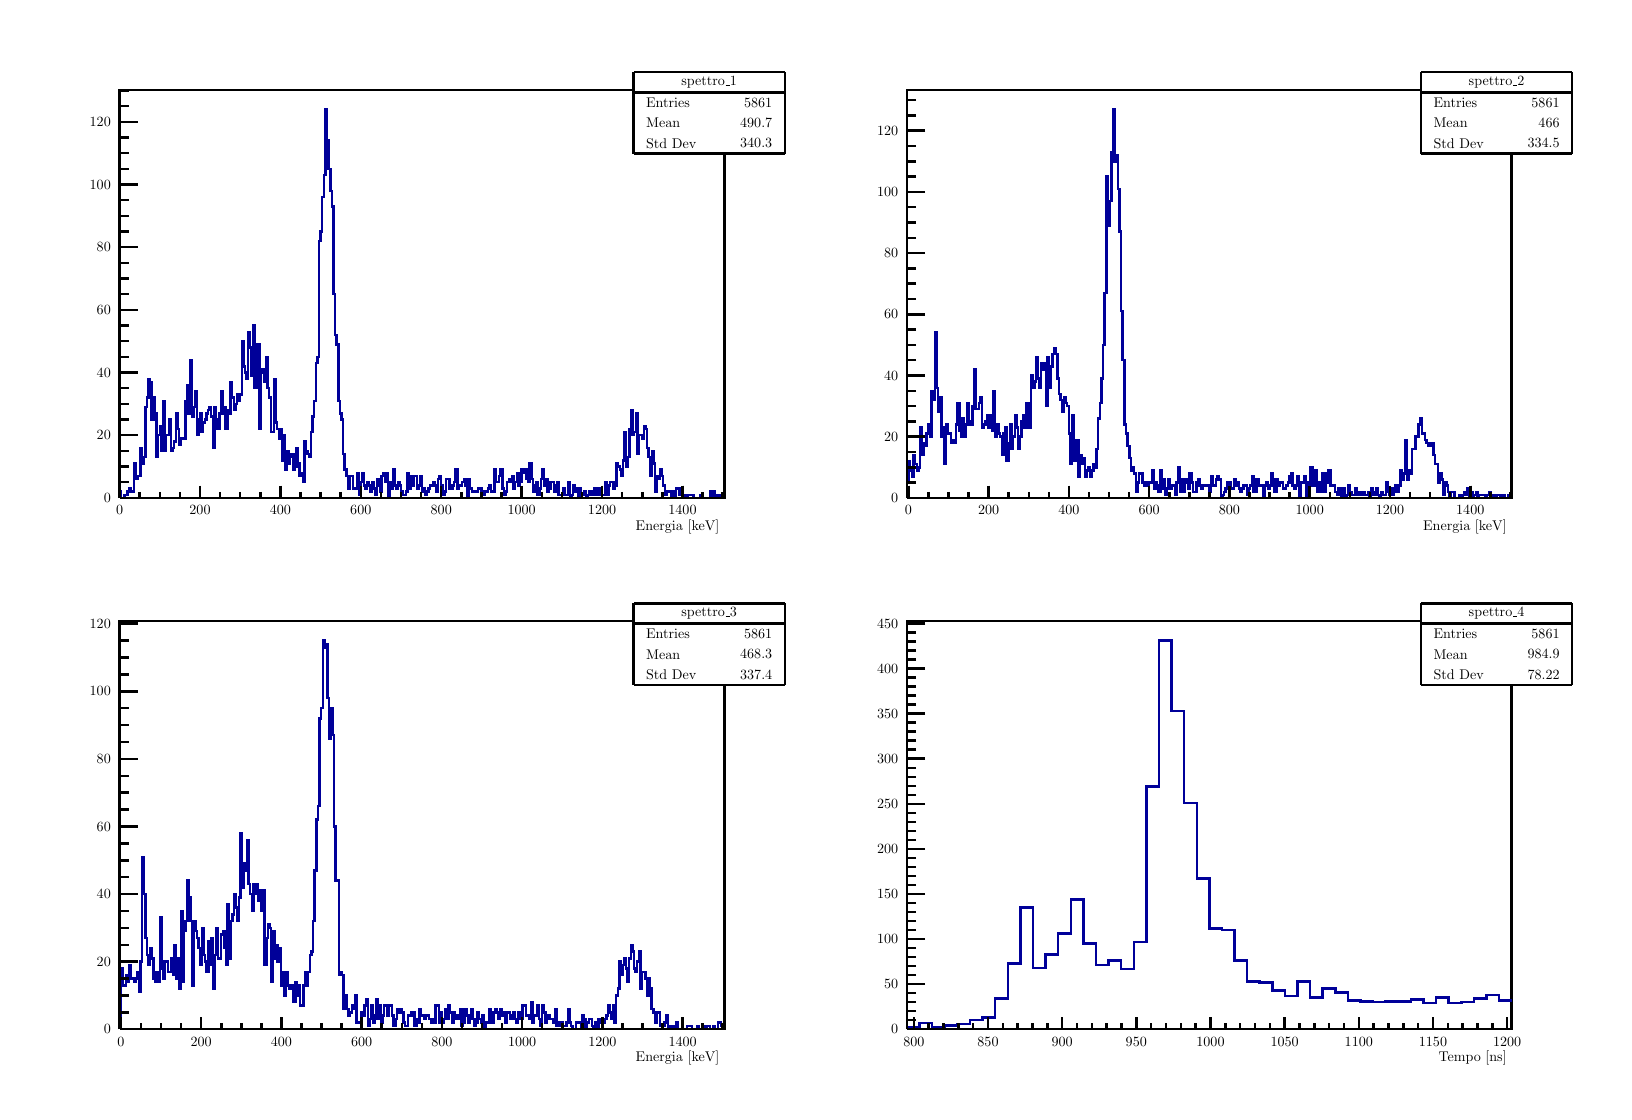
\begin{tikzpicture}
\pgfdeclareplotmark{cross} {
\pgfpathmoveto{\pgfpoint{-0.3\pgfplotmarksize}{\pgfplotmarksize}}
\pgfpathlineto{\pgfpoint{+0.3\pgfplotmarksize}{\pgfplotmarksize}}
\pgfpathlineto{\pgfpoint{+0.3\pgfplotmarksize}{0.3\pgfplotmarksize}}
\pgfpathlineto{\pgfpoint{+1\pgfplotmarksize}{0.3\pgfplotmarksize}}
\pgfpathlineto{\pgfpoint{+1\pgfplotmarksize}{-0.3\pgfplotmarksize}}
\pgfpathlineto{\pgfpoint{+0.3\pgfplotmarksize}{-0.3\pgfplotmarksize}}
\pgfpathlineto{\pgfpoint{+0.3\pgfplotmarksize}{-1.\pgfplotmarksize}}
\pgfpathlineto{\pgfpoint{-0.3\pgfplotmarksize}{-1.\pgfplotmarksize}}
\pgfpathlineto{\pgfpoint{-0.3\pgfplotmarksize}{-0.3\pgfplotmarksize}}
\pgfpathlineto{\pgfpoint{-1.\pgfplotmarksize}{-0.3\pgfplotmarksize}}
\pgfpathlineto{\pgfpoint{-1.\pgfplotmarksize}{0.3\pgfplotmarksize}}
\pgfpathlineto{\pgfpoint{-0.3\pgfplotmarksize}{0.3\pgfplotmarksize}}
\pgfpathclose
\pgfusepathqstroke
}
\pgfdeclareplotmark{cross*} {
\pgfpathmoveto{\pgfpoint{-0.3\pgfplotmarksize}{\pgfplotmarksize}}
\pgfpathlineto{\pgfpoint{+0.3\pgfplotmarksize}{\pgfplotmarksize}}
\pgfpathlineto{\pgfpoint{+0.3\pgfplotmarksize}{0.3\pgfplotmarksize}}
\pgfpathlineto{\pgfpoint{+1\pgfplotmarksize}{0.3\pgfplotmarksize}}
\pgfpathlineto{\pgfpoint{+1\pgfplotmarksize}{-0.3\pgfplotmarksize}}
\pgfpathlineto{\pgfpoint{+0.3\pgfplotmarksize}{-0.3\pgfplotmarksize}}
\pgfpathlineto{\pgfpoint{+0.3\pgfplotmarksize}{-1.\pgfplotmarksize}}
\pgfpathlineto{\pgfpoint{-0.3\pgfplotmarksize}{-1.\pgfplotmarksize}}
\pgfpathlineto{\pgfpoint{-0.3\pgfplotmarksize}{-0.3\pgfplotmarksize}}
\pgfpathlineto{\pgfpoint{-1.\pgfplotmarksize}{-0.3\pgfplotmarksize}}
\pgfpathlineto{\pgfpoint{-1.\pgfplotmarksize}{0.3\pgfplotmarksize}}
\pgfpathlineto{\pgfpoint{-0.3\pgfplotmarksize}{0.3\pgfplotmarksize}}
\pgfpathclose
\pgfusepathqfillstroke
}
\pgfdeclareplotmark{newstar} {
\pgfpathmoveto{\pgfqpoint{0pt}{\pgfplotmarksize}}
\pgfpathlineto{\pgfqpointpolar{44}{0.5\pgfplotmarksize}}
\pgfpathlineto{\pgfqpointpolar{18}{\pgfplotmarksize}}
\pgfpathlineto{\pgfqpointpolar{-20}{0.5\pgfplotmarksize}}
\pgfpathlineto{\pgfqpointpolar{-54}{\pgfplotmarksize}}
\pgfpathlineto{\pgfqpointpolar{-90}{0.5\pgfplotmarksize}}
\pgfpathlineto{\pgfqpointpolar{234}{\pgfplotmarksize}}
\pgfpathlineto{\pgfqpointpolar{198}{0.5\pgfplotmarksize}}
\pgfpathlineto{\pgfqpointpolar{162}{\pgfplotmarksize}}
\pgfpathlineto{\pgfqpointpolar{134}{0.5\pgfplotmarksize}}
\pgfpathclose
\pgfusepathqstroke
}
\pgfdeclareplotmark{newstar*} {
\pgfpathmoveto{\pgfqpoint{0pt}{\pgfplotmarksize}}
\pgfpathlineto{\pgfqpointpolar{44}{0.5\pgfplotmarksize}}
\pgfpathlineto{\pgfqpointpolar{18}{\pgfplotmarksize}}
\pgfpathlineto{\pgfqpointpolar{-20}{0.5\pgfplotmarksize}}
\pgfpathlineto{\pgfqpointpolar{-54}{\pgfplotmarksize}}
\pgfpathlineto{\pgfqpointpolar{-90}{0.5\pgfplotmarksize}}
\pgfpathlineto{\pgfqpointpolar{234}{\pgfplotmarksize}}
\pgfpathlineto{\pgfqpointpolar{198}{0.5\pgfplotmarksize}}
\pgfpathlineto{\pgfqpointpolar{162}{\pgfplotmarksize}}
\pgfpathlineto{\pgfqpointpolar{134}{0.5\pgfplotmarksize}}
\pgfpathclose
\pgfusepathqfillstroke
}
\definecolor{c}{rgb}{1,1,1};
\draw [color=c, fill=c] (0,0) rectangle (20,13.4957);
\draw [color=c, fill=c] (0.2,6.88281) rectangle (9.8,13.3607);
\draw [color=c, fill=c] (1.16,7.5306) rectangle (8.84,12.713);
\definecolor{c}{rgb}{0,0,0};
\draw [c,line width=0.9] (1.16,7.5306) -- (1.16,12.713) -- (8.84,12.713) -- (8.84,7.5306) -- (1.16,7.5306);
\definecolor{c}{rgb}{1,1,1};
\draw [color=c, fill=c] (1.16,7.5306) rectangle (8.84,12.713);
\definecolor{c}{rgb}{0,0,0};
\draw [c,line width=0.9] (1.16,7.5306) -- (1.16,12.713) -- (8.84,12.713) -- (8.84,7.5306) -- (1.16,7.5306);
\definecolor{c}{rgb}{0,0,0.6};
\draw [c,line width=0.9] (1.16,7.61021) -- (1.18043,7.61021) -- (1.18043,7.5306) -- (1.20085,7.5306) -- (1.20085,7.5306) -- (1.22128,7.5306) -- (1.22128,7.5704) -- (1.2417,7.5704) -- (1.2417,7.5704) -- (1.26213,7.5704) -- (1.26213,7.61021) --
 (1.28255,7.61021) -- (1.28255,7.65001) -- (1.30298,7.65001) -- (1.30298,7.61021) -- (1.3234,7.61021) -- (1.3234,7.61021) -- (1.34383,7.61021) -- (1.34383,7.96843) -- (1.36426,7.96843) -- (1.36426,7.76942) -- (1.38468,7.76942) -- (1.38468,7.80922) --
 (1.40511,7.80922) -- (1.40511,7.80922) -- (1.42553,7.80922) -- (1.42553,8.16745) -- (1.44596,8.16745) -- (1.44596,7.96843) -- (1.46638,7.96843) -- (1.46638,8.04804) -- (1.48681,8.04804) -- (1.48681,8.68489) -- (1.50723,8.68489) -- (1.50723,8.8043)
 -- (1.52766,8.8043) -- (1.52766,9.04312) -- (1.54809,9.04312) -- (1.54809,9.00331) -- (1.56851,9.00331) -- (1.56851,8.52568) -- (1.58894,8.52568) -- (1.58894,8.8043) -- (1.60936,8.8043) -- (1.60936,8.60528) -- (1.62979,8.60528) -- (1.62979,8.04804)
 -- (1.65021,8.04804) -- (1.65021,8.32666) -- (1.67064,8.32666) -- (1.67064,8.44607) -- (1.69106,8.44607) -- (1.69106,8.12765) -- (1.71149,8.12765) -- (1.71149,8.76449) -- (1.73191,8.76449) -- (1.73191,8.12765) -- (1.75234,8.12765) --
 (1.75234,8.32666) -- (1.77277,8.32666) -- (1.77277,8.32666) -- (1.79319,8.32666) -- (1.79319,8.52568) -- (1.81362,8.52568) -- (1.81362,8.12765) -- (1.83404,8.12765) -- (1.83404,8.16745) -- (1.85447,8.16745) -- (1.85447,8.24706) -- (1.87489,8.24706)
 -- (1.87489,8.60528) -- (1.89532,8.60528) -- (1.89532,8.40627) -- (1.91574,8.40627) -- (1.91574,8.20725) -- (1.93617,8.20725) -- (1.93617,8.28686) -- (1.9566,8.28686) -- (1.9566,8.28686) -- (1.97702,8.28686) -- (1.97702,8.28686) -- (1.99745,8.28686)
 -- (1.99745,8.76449) -- (2.01787,8.76449) -- (2.01787,8.96351) -- (2.0383,8.96351) -- (2.0383,8.60528) -- (2.05872,8.60528) -- (2.05872,9.28193) -- (2.07915,9.28193) -- (2.07915,8.56548) -- (2.09957,8.56548) -- (2.09957,8.68489) -- (2.12,8.68489) --
 (2.12,8.8839) -- (2.14043,8.8839) -- (2.14043,8.32666) -- (2.16085,8.32666) -- (2.16085,8.52568) -- (2.18128,8.52568) -- (2.18128,8.60528) -- (2.2017,8.60528) -- (2.2017,8.36646) -- (2.22213,8.36646) -- (2.22213,8.48587) -- (2.24255,8.48587) --
 (2.24255,8.52568) -- (2.26298,8.52568) -- (2.26298,8.60528) -- (2.2834,8.60528) -- (2.2834,8.64509) -- (2.30383,8.64509) -- (2.30383,8.68489) -- (2.32426,8.68489) -- (2.32426,8.56548) -- (2.34468,8.56548) -- (2.34468,8.16745) -- (2.36511,8.16745) --
 (2.36511,8.68489) -- (2.38553,8.68489) -- (2.38553,8.52568) -- (2.40596,8.52568) -- (2.40596,8.40627) -- (2.42638,8.40627) -- (2.42638,8.60528) -- (2.44681,8.60528) -- (2.44681,8.8839) -- (2.46723,8.8839) -- (2.46723,8.60528) -- (2.48766,8.60528) --
 (2.48766,8.68489) -- (2.50809,8.68489) -- (2.50809,8.40627) -- (2.52851,8.40627) -- (2.52851,8.64509) -- (2.54894,8.64509) -- (2.54894,8.60528) -- (2.56936,8.60528) -- (2.56936,9.00331) -- (2.58979,9.00331) -- (2.58979,8.8043) -- (2.61021,8.8043) --
 (2.61021,8.64509) -- (2.63064,8.64509) -- (2.63064,8.72469) -- (2.65106,8.72469) -- (2.65106,8.8441) -- (2.67149,8.8441) -- (2.67149,8.76449) -- (2.69192,8.76449) -- (2.69192,8.8441) -- (2.71234,8.8441) -- (2.71234,9.52075) -- (2.73277,9.52075) --
 (2.73277,9.20233) -- (2.75319,9.20233) -- (2.75319,9.12272) -- (2.77362,9.12272) -- (2.77362,9.04312) -- (2.79404,9.04312) -- (2.79404,9.64016) -- (2.81447,9.64016) -- (2.81447,9.44114) -- (2.83489,9.44114) -- (2.83489,9.08292) -- (2.85532,9.08292)
 -- (2.85532,9.71977) -- (2.87574,9.71977) -- (2.87574,8.92371) -- (2.89617,8.92371) -- (2.89617,9.48095) -- (2.9166,9.48095) -- (2.9166,9.48095) -- (2.93702,9.48095) -- (2.93702,8.40627) -- (2.95745,8.40627) -- (2.95745,9.12272) -- (2.97787,9.12272)
 -- (2.97787,9.16252) -- (2.9983,9.16252) -- (2.9983,9.00331) -- (3.01872,9.00331) -- (3.01872,9.32174) -- (3.03915,9.32174) -- (3.03915,8.92371) -- (3.05957,8.92371) -- (3.05957,8.8043) -- (3.08,8.8043) -- (3.08,8.36646) -- (3.10043,8.36646) --
 (3.10043,8.36646) -- (3.12085,8.36646) -- (3.12085,9.04312) -- (3.14128,9.04312) -- (3.14128,8.48587) -- (3.1617,8.48587) -- (3.1617,8.40627) -- (3.18213,8.40627) -- (3.18213,8.28686) -- (3.20255,8.28686) -- (3.20255,8.40627) -- (3.22298,8.40627) --
 (3.22298,8.00824) -- (3.2434,8.00824) -- (3.2434,8.32666) -- (3.26383,8.32666) -- (3.26383,7.88883) -- (3.28426,7.88883) -- (3.28426,8.12765) -- (3.30468,8.12765) -- (3.30468,7.96843) -- (3.32511,7.96843) -- (3.32511,8.04804) -- (3.34553,8.04804) --
 (3.34553,8.08784) -- (3.36596,8.08784) -- (3.36596,7.88883) -- (3.38638,7.88883) -- (3.38638,7.92863) -- (3.40681,7.92863) -- (3.40681,8.16745) -- (3.42723,8.16745) -- (3.42723,7.96843) -- (3.44766,7.96843) -- (3.44766,7.80922) -- (3.46809,7.80922)
 -- (3.46809,7.84903) -- (3.48851,7.84903) -- (3.48851,7.72962) -- (3.50894,7.72962) -- (3.50894,8.24706) -- (3.52936,8.24706) -- (3.52936,8.12765) -- (3.54979,8.12765) -- (3.54979,8.08784) -- (3.57021,8.08784) -- (3.57021,8.04804) --
 (3.59064,8.04804) -- (3.59064,8.36646) -- (3.61106,8.36646) -- (3.61106,8.56548) -- (3.63149,8.56548) -- (3.63149,8.76449) -- (3.65191,8.76449) -- (3.65191,9.24213) -- (3.67234,9.24213) -- (3.67234,9.32174) -- (3.69277,9.32174) -- (3.69277,10.7944)
 -- (3.71319,10.7944) -- (3.71319,10.9139) -- (3.73362,10.9139) -- (3.73362,11.3517) -- (3.75404,11.3517) -- (3.75404,11.6303) -- (3.77447,11.6303) -- (3.77447,12.4662) -- (3.79489,12.4662) -- (3.79489,12.0681) -- (3.81532,12.0681) --
 (3.81532,11.7099) -- (3.83574,11.7099) -- (3.83574,11.4313) -- (3.85617,11.4313) -- (3.85617,11.2323) -- (3.8766,11.2323) -- (3.8766,10.1178) -- (3.89702,10.1178) -- (3.89702,9.60036) -- (3.91745,9.60036) -- (3.91745,9.48095) -- (3.93787,9.48095) --
 (3.93787,8.76449) -- (3.9583,8.76449) -- (3.9583,8.60528) -- (3.97872,8.60528) -- (3.97872,8.52568) -- (3.99915,8.52568) -- (3.99915,8.08784) -- (4.01957,8.08784) -- (4.01957,7.88883) -- (4.04,7.88883) -- (4.04,7.80922) -- (4.06043,7.80922) --
 (4.06043,7.65001) -- (4.08085,7.65001) -- (4.08085,7.80922) -- (4.10128,7.80922) -- (4.10128,7.80922) -- (4.1217,7.80922) -- (4.1217,7.65001) -- (4.14213,7.65001) -- (4.14213,7.65001) -- (4.16255,7.65001) -- (4.16255,7.65001) -- (4.18298,7.65001) --
 (4.18298,7.84903) -- (4.2034,7.84903) -- (4.2034,7.5704) -- (4.22383,7.5704) -- (4.22383,7.72962) -- (4.24426,7.72962) -- (4.24426,7.84903) -- (4.26468,7.84903) -- (4.26468,7.68981) -- (4.28511,7.68981) -- (4.28511,7.65001) -- (4.30553,7.65001) --
 (4.30553,7.72962) -- (4.32596,7.72962) -- (4.32596,7.68981) -- (4.34638,7.68981) -- (4.34638,7.61021) -- (4.36681,7.61021) -- (4.36681,7.72962) -- (4.38723,7.72962) -- (4.38723,7.65001) -- (4.40766,7.65001) -- (4.40766,7.5704) -- (4.42809,7.5704) --
 (4.42809,7.76942) -- (4.44851,7.76942) -- (4.44851,7.68981) -- (4.46894,7.68981) -- (4.46894,7.61021) -- (4.48936,7.61021) -- (4.48936,7.80922) -- (4.50979,7.80922) -- (4.50979,7.84903) -- (4.53021,7.84903) -- (4.53021,7.72962) -- (4.55064,7.72962)
 -- (4.55064,7.84903) -- (4.57106,7.84903) -- (4.57106,7.5306) -- (4.59149,7.5306) -- (4.59149,7.72962) -- (4.61192,7.72962) -- (4.61192,7.65001) -- (4.63234,7.65001) -- (4.63234,7.88883) -- (4.65277,7.88883) -- (4.65277,7.68981) -- (4.67319,7.68981)
 -- (4.67319,7.65001) -- (4.69362,7.65001) -- (4.69362,7.72962) -- (4.71404,7.72962) -- (4.71404,7.68981) -- (4.73447,7.68981) -- (4.73447,7.61021) -- (4.75489,7.61021) -- (4.75489,7.5704) -- (4.77532,7.5704) -- (4.77532,7.5704) -- (4.79574,7.5704)
 -- (4.79574,7.61021) -- (4.81617,7.61021) -- (4.81617,7.84903) -- (4.8366,7.84903) -- (4.8366,7.65001) -- (4.85702,7.65001) -- (4.85702,7.80922) -- (4.87745,7.80922) -- (4.87745,7.68981) -- (4.89787,7.68981) -- (4.89787,7.80922) -- (4.9183,7.80922)
 -- (4.9183,7.80922) -- (4.93872,7.80922) -- (4.93872,7.65001) -- (4.95915,7.65001) -- (4.95915,7.68981) -- (4.97957,7.68981) -- (4.97957,7.80922) -- (5,7.80922) -- (5,7.61021) -- (5.02043,7.61021) -- (5.02043,7.65001) -- (5.04085,7.65001) --
 (5.04085,7.5704) -- (5.06128,7.5704) -- (5.06128,7.61021) -- (5.0817,7.61021) -- (5.0817,7.65001) -- (5.10213,7.65001) -- (5.10213,7.68981) -- (5.12255,7.68981) -- (5.12255,7.68981) -- (5.14298,7.68981) -- (5.14298,7.72962) -- (5.1634,7.72962) --
 (5.1634,7.68981) -- (5.18383,7.68981) -- (5.18383,7.61021) -- (5.20426,7.61021) -- (5.20426,7.76942) -- (5.22468,7.76942) -- (5.22468,7.80922) -- (5.24511,7.80922) -- (5.24511,7.68981) -- (5.26553,7.68981) -- (5.26553,7.5704) -- (5.28596,7.5704) --
 (5.28596,7.61021) -- (5.30638,7.61021) -- (5.30638,7.76942) -- (5.32681,7.76942) -- (5.32681,7.76942) -- (5.34723,7.76942) -- (5.34723,7.65001) -- (5.36766,7.65001) -- (5.36766,7.65001) -- (5.38808,7.65001) -- (5.38808,7.68981) -- (5.40851,7.68981)
 -- (5.40851,7.72962) -- (5.42894,7.72962) -- (5.42894,7.88883) -- (5.44936,7.88883) -- (5.44936,7.65001) -- (5.46979,7.65001) -- (5.46979,7.68981) -- (5.49021,7.68981) -- (5.49021,7.68981) -- (5.51064,7.68981) -- (5.51064,7.72962) --
 (5.53106,7.72962) -- (5.53106,7.76942) -- (5.55149,7.76942) -- (5.55149,7.68981) -- (5.57191,7.68981) -- (5.57191,7.5306) -- (5.59234,7.5306) -- (5.59234,7.76942) -- (5.61277,7.76942) -- (5.61277,7.65001) -- (5.63319,7.65001) -- (5.63319,7.61021) --
 (5.65362,7.61021) -- (5.65362,7.61021) -- (5.67404,7.61021) -- (5.67404,7.61021) -- (5.69447,7.61021) -- (5.69447,7.61021) -- (5.71489,7.61021) -- (5.71489,7.65001) -- (5.73532,7.65001) -- (5.73532,7.65001) -- (5.75574,7.65001) -- (5.75574,7.61021)
 -- (5.77617,7.61021) -- (5.77617,7.5704) -- (5.7966,7.5704) -- (5.7966,7.61021) -- (5.81702,7.61021) -- (5.81702,7.61021) -- (5.83745,7.61021) -- (5.83745,7.65001) -- (5.85787,7.65001) -- (5.85787,7.68981) -- (5.8783,7.68981) -- (5.8783,7.61021) --
 (5.89872,7.61021) -- (5.89872,7.61021) -- (5.91915,7.61021) -- (5.91915,7.88883) -- (5.93957,7.88883) -- (5.93957,7.72962) -- (5.96,7.72962) -- (5.96,7.72962) -- (5.98043,7.72962) -- (5.98043,7.80922) -- (6.00085,7.80922) -- (6.00085,7.88883) --
 (6.02128,7.88883) -- (6.02128,7.65001) -- (6.0417,7.65001) -- (6.0417,7.5704) -- (6.06213,7.5704) -- (6.06213,7.61021) -- (6.08255,7.61021) -- (6.08255,7.72962) -- (6.10298,7.72962) -- (6.10298,7.76942) -- (6.1234,7.76942) -- (6.1234,7.72962) --
 (6.14383,7.72962) -- (6.14383,7.80922) -- (6.16426,7.80922) -- (6.16426,7.65001) -- (6.18468,7.65001) -- (6.18468,7.72962) -- (6.20511,7.72962) -- (6.20511,7.84903) -- (6.22553,7.84903) -- (6.22553,7.68981) -- (6.24596,7.68981) -- (6.24596,7.72962)
 -- (6.26638,7.72962) -- (6.26638,7.88883) -- (6.28681,7.88883) -- (6.28681,7.84903) -- (6.30723,7.84903) -- (6.30723,7.88883) -- (6.32766,7.88883) -- (6.32766,7.76942) -- (6.34808,7.76942) -- (6.34808,7.72962) -- (6.36851,7.72962) --
 (6.36851,7.96843) -- (6.38894,7.96843) -- (6.38894,7.76942) -- (6.40936,7.76942) -- (6.40936,7.61021) -- (6.42979,7.61021) -- (6.42979,7.68981) -- (6.45021,7.68981) -- (6.45021,7.72962) -- (6.47064,7.72962) -- (6.47064,7.5704) -- (6.49106,7.5704) --
 (6.49106,7.65001) -- (6.51149,7.65001) -- (6.51149,7.76942) -- (6.53191,7.76942) -- (6.53191,7.88883) -- (6.55234,7.88883) -- (6.55234,7.68981) -- (6.57277,7.68981) -- (6.57277,7.76942) -- (6.59319,7.76942) -- (6.59319,7.61021) -- (6.61362,7.61021)
 -- (6.61362,7.65001) -- (6.63404,7.65001) -- (6.63404,7.72962) -- (6.65447,7.72962) -- (6.65447,7.72962) -- (6.67489,7.72962) -- (6.67489,7.61021) -- (6.69532,7.61021) -- (6.69532,7.68981) -- (6.71574,7.68981) -- (6.71574,7.72962) --
 (6.73617,7.72962) -- (6.73617,7.5704) -- (6.7566,7.5704) -- (6.7566,7.5704) -- (6.77702,7.5704) -- (6.77702,7.5704) -- (6.79745,7.5704) -- (6.79745,7.65001) -- (6.81787,7.65001) -- (6.81787,7.5704) -- (6.8383,7.5704) -- (6.8383,7.5704) --
 (6.85872,7.5704) -- (6.85872,7.72962) -- (6.87915,7.72962) -- (6.87915,7.5306) -- (6.89957,7.5306) -- (6.89957,7.5704) -- (6.92,7.5704) -- (6.92,7.68981) -- (6.94043,7.68981) -- (6.94043,7.61021) -- (6.96085,7.61021) -- (6.96085,7.65001) --
 (6.98128,7.65001) -- (6.98128,7.5306) -- (7.0017,7.5306) -- (7.0017,7.65001) -- (7.02213,7.65001) -- (7.02213,7.5704) -- (7.04255,7.5704) -- (7.04255,7.5704) -- (7.06298,7.5704) -- (7.06298,7.61021) -- (7.0834,7.61021) -- (7.0834,7.5306) --
 (7.10383,7.5306) -- (7.10383,7.5704) -- (7.12426,7.5704) -- (7.12426,7.61021) -- (7.14468,7.61021) -- (7.14468,7.5704) -- (7.16511,7.5704) -- (7.16511,7.61021) -- (7.18553,7.61021) -- (7.18553,7.65001) -- (7.20596,7.65001) -- (7.20596,7.5704) --
 (7.22638,7.5704) -- (7.22638,7.65001) -- (7.24681,7.65001) -- (7.24681,7.5704) -- (7.26723,7.5704) -- (7.26723,7.65001) -- (7.28766,7.65001) -- (7.28766,7.5704) -- (7.30808,7.5704) -- (7.30808,7.5704) -- (7.32851,7.5704) -- (7.32851,7.72962) --
 (7.34894,7.72962) -- (7.34894,7.5704) -- (7.36936,7.5704) -- (7.36936,7.68981) -- (7.38979,7.68981) -- (7.38979,7.72962) -- (7.41021,7.72962) -- (7.41021,7.72962) -- (7.43064,7.72962) -- (7.43064,7.65001) -- (7.45106,7.65001) -- (7.45106,7.68981) --
 (7.47149,7.68981) -- (7.47149,7.96843) -- (7.49191,7.96843) -- (7.49191,7.92863) -- (7.51234,7.92863) -- (7.51234,7.88883) -- (7.53277,7.88883) -- (7.53277,7.80922) -- (7.55319,7.80922) -- (7.55319,8.00824) -- (7.57362,8.00824) -- (7.57362,8.36646)
 -- (7.59404,8.36646) -- (7.59404,7.92863) -- (7.61447,7.92863) -- (7.61447,8.04804) -- (7.63489,8.04804) -- (7.63489,8.40627) -- (7.65532,8.40627) -- (7.65532,8.64509) -- (7.67574,8.64509) -- (7.67574,8.32666) -- (7.69617,8.32666) --
 (7.69617,8.36646) -- (7.7166,8.36646) -- (7.7166,8.60528) -- (7.73702,8.60528) -- (7.73702,8.08784) -- (7.75745,8.08784) -- (7.75745,8.32666) -- (7.77787,8.32666) -- (7.77787,8.32666) -- (7.7983,8.32666) -- (7.7983,8.28686) -- (7.81872,8.28686) --
 (7.81872,8.44607) -- (7.83915,8.44607) -- (7.83915,8.40627) -- (7.85957,8.40627) -- (7.85957,8.16745) -- (7.88,8.16745) -- (7.88,8.04804) -- (7.90043,8.04804) -- (7.90043,7.80922) -- (7.92085,7.80922) -- (7.92085,8.12765) -- (7.94128,8.12765) --
 (7.94128,7.96843) -- (7.9617,7.96843) -- (7.9617,7.61021) -- (7.98213,7.61021) -- (7.98213,7.80922) -- (8.00255,7.80922) -- (8.00255,7.76942) -- (8.02298,7.76942) -- (8.02298,7.88883) -- (8.0434,7.88883) -- (8.0434,7.80922) -- (8.06383,7.80922) --
 (8.06383,7.68981) -- (8.08426,7.68981) -- (8.08426,7.5704) -- (8.10468,7.5704) -- (8.10468,7.61021) -- (8.12511,7.61021) -- (8.12511,7.61021) -- (8.14553,7.61021) -- (8.14553,7.61021) -- (8.16596,7.61021) -- (8.16596,7.5306) -- (8.18638,7.5306) --
 (8.18638,7.61021) -- (8.20681,7.61021) -- (8.20681,7.5306) -- (8.22723,7.5306) -- (8.22723,7.65001) -- (8.24766,7.65001) -- (8.24766,7.65001) -- (8.26809,7.65001) -- (8.26809,7.5704) -- (8.28851,7.5704) -- (8.28851,7.61021) -- (8.30894,7.61021) --
 (8.30894,7.5306) -- (8.32936,7.5306) -- (8.32936,7.5704) -- (8.34979,7.5704) -- (8.34979,7.5306) -- (8.37021,7.5306) -- (8.37021,7.5704) -- (8.39064,7.5704) -- (8.39064,7.5704) -- (8.41106,7.5704) -- (8.41106,7.5704) -- (8.43149,7.5704) --
 (8.43149,7.5704) -- (8.45191,7.5704) -- (8.45191,7.5306) -- (8.47234,7.5306) -- (8.47234,7.5306) -- (8.49277,7.5306) -- (8.49277,7.5306) -- (8.51319,7.5306) -- (8.51319,7.5306) -- (8.53362,7.5306) -- (8.53362,7.5704) -- (8.55404,7.5704) --
 (8.55404,7.5306) -- (8.57447,7.5306) -- (8.57447,7.5306) -- (8.59489,7.5306) -- (8.59489,7.5306) -- (8.61532,7.5306) -- (8.61532,7.5306) -- (8.63575,7.5306) -- (8.63575,7.5306) -- (8.65617,7.5306) -- (8.65617,7.61021) -- (8.6766,7.61021) --
 (8.6766,7.5306) -- (8.69702,7.5306) -- (8.69702,7.61021) -- (8.71745,7.61021) -- (8.71745,7.5306) -- (8.73787,7.5306) -- (8.73787,7.5704) -- (8.7583,7.5704) -- (8.7583,7.5306) -- (8.77872,7.5306) -- (8.77872,7.5704) -- (8.79915,7.5704) --
 (8.79915,7.5306) -- (8.81957,7.5306) -- (8.81957,7.5704) -- (8.84,7.5704);
\definecolor{c}{rgb}{1,1,1};
\draw [color=c, fill=c] (7.688,11.9032) rectangle (9.608,12.9397);
\definecolor{c}{rgb}{0,0,0};
\draw [c,line width=0.9] (7.688,11.9032) -- (9.608,11.9032);
\draw [c,line width=0.9] (9.608,11.9032) -- (9.608,12.9397);
\draw [c,line width=0.9] (9.608,12.9397) -- (7.688,12.9397);
\draw [c,line width=0.9] (7.688,12.9397) -- (7.688,11.9032);
\draw (8.648,12.8101) node[scale=0.509285, color=c, rotate=0]{spettro\_1};
\draw [c,line width=0.9] (7.688,12.6806) -- (9.608,12.6806);
\draw [anchor= west] (7.784,12.551) node[scale=0.509285, color=c, rotate=0]{Entries };
\draw [anchor= east] (9.512,12.551) node[scale=0.509285, color=c, rotate=0]{ 5861};
\draw [anchor= west] (7.784,12.2919) node[scale=0.509285, color=c, rotate=0]{Mean  };
\draw [anchor= east] (9.512,12.2919) node[scale=0.509285, color=c, rotate=0]{  490.7};
\draw [anchor= west] (7.784,12.0328) node[scale=0.509285, color=c, rotate=0]{Std Dev   };
\draw [anchor= east] (9.512,12.0328) node[scale=0.509285, color=c, rotate=0]{  340.3};
\draw [c,line width=0.9] (1.16,7.5306) -- (8.84,7.5306);
\draw [anchor= east] (8.84,7.16784) node[scale=0.509285, color=c, rotate=0]{Energia [keV]};
\draw [c,line width=0.9] (1.1601,7.68607) -- (1.1601,7.5306);
\draw [c,line width=0.9] (1.41542,7.60834) -- (1.41542,7.5306);
\draw [c,line width=0.9] (1.67074,7.60834) -- (1.67074,7.5306);
\draw [c,line width=0.9] (1.92606,7.60834) -- (1.92606,7.5306);
\draw [c,line width=0.9] (2.18138,7.68607) -- (2.18138,7.5306);
\draw [c,line width=0.9] (2.4367,7.60834) -- (2.4367,7.5306);
\draw [c,line width=0.9] (2.69202,7.60834) -- (2.69202,7.5306);
\draw [c,line width=0.9] (2.94734,7.60834) -- (2.94734,7.5306);
\draw [c,line width=0.9] (3.20266,7.68607) -- (3.20266,7.5306);
\draw [c,line width=0.9] (3.45798,7.60834) -- (3.45798,7.5306);
\draw [c,line width=0.9] (3.7133,7.60834) -- (3.7133,7.5306);
\draw [c,line width=0.9] (3.96862,7.60834) -- (3.96862,7.5306);
\draw [c,line width=0.9] (4.22394,7.68607) -- (4.22394,7.5306);
\draw [c,line width=0.9] (4.47925,7.60834) -- (4.47925,7.5306);
\draw [c,line width=0.9] (4.73457,7.60834) -- (4.73457,7.5306);
\draw [c,line width=0.9] (4.98989,7.60834) -- (4.98989,7.5306);
\draw [c,line width=0.9] (5.24521,7.68607) -- (5.24521,7.5306);
\draw [c,line width=0.9] (5.50053,7.60834) -- (5.50053,7.5306);
\draw [c,line width=0.9] (5.75585,7.60834) -- (5.75585,7.5306);
\draw [c,line width=0.9] (6.01117,7.60834) -- (6.01117,7.5306);
\draw [c,line width=0.9] (6.26649,7.68607) -- (6.26649,7.5306);
\draw [c,line width=0.9] (6.52181,7.60834) -- (6.52181,7.5306);
\draw [c,line width=0.9] (6.77713,7.60834) -- (6.77713,7.5306);
\draw [c,line width=0.9] (7.03245,7.60834) -- (7.03245,7.5306);
\draw [c,line width=0.9] (7.28777,7.68607) -- (7.28777,7.5306);
\draw [c,line width=0.9] (7.54309,7.60834) -- (7.54309,7.5306);
\draw [c,line width=0.9] (7.79841,7.60834) -- (7.79841,7.5306);
\draw [c,line width=0.9] (8.05373,7.60834) -- (8.05373,7.5306);
\draw [c,line width=0.9] (8.30905,7.68607) -- (8.30905,7.5306);
\draw [c,line width=0.9] (1.1601,7.68607) -- (1.1601,7.5306);
\draw [c,line width=0.9] (8.30905,7.68607) -- (8.30905,7.5306);
\draw [c,line width=0.9] (8.56436,7.60834) -- (8.56436,7.5306);
\draw [c,line width=0.9] (8.81968,7.60834) -- (8.81968,7.5306);
\draw [anchor=base] (1.1601,7.31683) node[scale=0.509285, color=c, rotate=0]{0};
\draw [anchor=base] (2.18138,7.31683) node[scale=0.509285, color=c, rotate=0]{200};
\draw [anchor=base] (3.20266,7.31683) node[scale=0.509285, color=c, rotate=0]{400};
\draw [anchor=base] (4.22394,7.31683) node[scale=0.509285, color=c, rotate=0]{600};
\draw [anchor=base] (5.24521,7.31683) node[scale=0.509285, color=c, rotate=0]{800};
\draw [anchor=base] (6.26649,7.31683) node[scale=0.509285, color=c, rotate=0]{1000};
\draw [anchor=base] (7.28777,7.31683) node[scale=0.509285, color=c, rotate=0]{1200};
\draw [anchor=base] (8.30905,7.31683) node[scale=0.509285, color=c, rotate=0]{1400};
\draw [c,line width=0.9] (1.16,7.5306) -- (1.16,12.713);
\draw [c,line width=0.9] (1.3904,7.5306) -- (1.16,7.5306);
\draw [c,line width=0.9] (1.2752,7.72962) -- (1.16,7.72962);
\draw [c,line width=0.9] (1.2752,7.92863) -- (1.16,7.92863);
\draw [c,line width=0.9] (1.2752,8.12765) -- (1.16,8.12765);
\draw [c,line width=0.9] (1.3904,8.32666) -- (1.16,8.32666);
\draw [c,line width=0.9] (1.2752,8.52568) -- (1.16,8.52568);
\draw [c,line width=0.9] (1.2752,8.72469) -- (1.16,8.72469);
\draw [c,line width=0.9] (1.2752,8.92371) -- (1.16,8.92371);
\draw [c,line width=0.9] (1.3904,9.12272) -- (1.16,9.12272);
\draw [c,line width=0.9] (1.2752,9.32174) -- (1.16,9.32174);
\draw [c,line width=0.9] (1.2752,9.52075) -- (1.16,9.52075);
\draw [c,line width=0.9] (1.2752,9.71977) -- (1.16,9.71977);
\draw [c,line width=0.9] (1.3904,9.91878) -- (1.16,9.91878);
\draw [c,line width=0.9] (1.2752,10.1178) -- (1.16,10.1178);
\draw [c,line width=0.9] (1.2752,10.3168) -- (1.16,10.3168);
\draw [c,line width=0.9] (1.2752,10.5158) -- (1.16,10.5158);
\draw [c,line width=0.9] (1.3904,10.7148) -- (1.16,10.7148);
\draw [c,line width=0.9] (1.2752,10.9139) -- (1.16,10.9139);
\draw [c,line width=0.9] (1.2752,11.1129) -- (1.16,11.1129);
\draw [c,line width=0.9] (1.2752,11.3119) -- (1.16,11.3119);
\draw [c,line width=0.9] (1.3904,11.5109) -- (1.16,11.5109);
\draw [c,line width=0.9] (1.2752,11.7099) -- (1.16,11.7099);
\draw [c,line width=0.9] (1.2752,11.9089) -- (1.16,11.9089);
\draw [c,line width=0.9] (1.2752,12.1079) -- (1.16,12.1079);
\draw [c,line width=0.9] (1.3904,12.307) -- (1.16,12.307);
\draw [c,line width=0.9] (1.3904,12.307) -- (1.16,12.307);
\draw [c,line width=0.9] (1.2752,12.506) -- (1.16,12.506);
\draw [c,line width=0.9] (1.2752,12.705) -- (1.16,12.705);
\draw [anchor= east] (1.112,7.5306) node[scale=0.509285, color=c, rotate=0]{0};
\draw [anchor= east] (1.112,8.32666) node[scale=0.509285, color=c, rotate=0]{20};
\draw [anchor= east] (1.112,9.12272) node[scale=0.509285, color=c, rotate=0]{40};
\draw [anchor= east] (1.112,9.91878) node[scale=0.509285, color=c, rotate=0]{60};
\draw [anchor= east] (1.112,10.7148) node[scale=0.509285, color=c, rotate=0]{80};
\draw [anchor= east] (1.112,11.5109) node[scale=0.509285, color=c, rotate=0]{100};
\draw [anchor= east] (1.112,12.307) node[scale=0.509285, color=c, rotate=0]{120};
\definecolor{c}{rgb}{1,1,1};
\draw [color=c, fill=c] (7.688,11.9032) rectangle (9.608,12.9397);
\definecolor{c}{rgb}{0,0,0};
\draw [c,line width=0.9] (7.688,11.9032) -- (9.608,11.9032);
\draw [c,line width=0.9] (9.608,11.9032) -- (9.608,12.9397);
\draw [c,line width=0.9] (9.608,12.9397) -- (7.688,12.9397);
\draw [c,line width=0.9] (7.688,12.9397) -- (7.688,11.9032);
\draw (8.648,12.8101) node[scale=0.509285, color=c, rotate=0]{spettro\_1};
\draw [c,line width=0.9] (7.688,12.6806) -- (9.608,12.6806);
\draw [anchor= west] (7.784,12.551) node[scale=0.509285, color=c, rotate=0]{Entries };
\draw [anchor= east] (9.512,12.551) node[scale=0.509285, color=c, rotate=0]{ 5861};
\draw [anchor= west] (7.784,12.2919) node[scale=0.509285, color=c, rotate=0]{Mean  };
\draw [anchor= east] (9.512,12.2919) node[scale=0.509285, color=c, rotate=0]{  490.7};
\draw [anchor= west] (7.784,12.0328) node[scale=0.509285, color=c, rotate=0]{Std Dev   };
\draw [anchor= east] (9.512,12.0328) node[scale=0.509285, color=c, rotate=0]{  340.3};
\definecolor{c}{rgb}{1,1,1};
\draw [color=c, fill=c] (10.2,6.88281) rectangle (19.8,13.3607);
\draw [color=c, fill=c] (11.16,7.5306) rectangle (18.84,12.713);
\definecolor{c}{rgb}{0,0,0};
\draw [c,line width=0.9] (11.16,7.5306) -- (11.16,12.713) -- (18.84,12.713) -- (18.84,7.5306) -- (11.16,7.5306);
\definecolor{c}{rgb}{1,1,1};
\draw [color=c, fill=c] (11.16,7.5306) rectangle (18.84,12.713);
\definecolor{c}{rgb}{0,0,0};
\draw [c,line width=0.9] (11.16,7.5306) -- (11.16,12.713) -- (18.84,12.713) -- (18.84,7.5306) -- (11.16,7.5306);
\definecolor{c}{rgb}{0,0,0.6};
\draw [c,line width=0.9] (11.16,7.72492) -- (11.1808,7.72492) -- (11.1808,7.99695) -- (11.2015,7.99695) -- (11.2015,7.88037) -- (11.2223,7.88037) -- (11.2223,7.80264) -- (11.243,7.80264) -- (11.243,8.07468) -- (11.2638,8.07468) -- (11.2638,7.95809)
 -- (11.2845,7.95809) -- (11.2845,7.88037) -- (11.3053,7.88037) -- (11.3053,7.91923) -- (11.3261,7.91923) -- (11.3261,8.42445) -- (11.3468,8.42445) -- (11.3468,8.07468) -- (11.3676,8.07468) -- (11.3676,8.23013) -- (11.3883,8.23013) --
 (11.3883,8.19127) -- (11.4091,8.19127) -- (11.4091,8.34672) -- (11.4298,8.34672) -- (11.4298,8.46331) -- (11.4506,8.46331) -- (11.4506,8.30786) -- (11.4714,8.30786) -- (11.4714,8.8908) -- (11.4921,8.8908) -- (11.4921,8.77421) -- (11.5129,8.77421) --
 (11.5129,9.62919) -- (11.5336,9.62919) -- (11.5336,8.92966) -- (11.5544,8.92966) -- (11.5544,8.61876) -- (11.5751,8.61876) -- (11.5751,8.81307) -- (11.5959,8.81307) -- (11.5959,8.30786) -- (11.6166,8.30786) -- (11.6166,8.42445) -- (11.6374,8.42445)
 -- (11.6374,7.95809) -- (11.6582,7.95809) -- (11.6582,8.46331) -- (11.6789,8.46331) -- (11.6789,8.34672) -- (11.6997,8.34672) -- (11.6997,8.34672) -- (11.7204,8.34672) -- (11.7204,8.23013) -- (11.7412,8.23013) -- (11.7412,8.26899) --
 (11.7619,8.26899) -- (11.7619,8.23013) -- (11.7827,8.23013) -- (11.7827,8.46331) -- (11.8035,8.46331) -- (11.8035,8.73535) -- (11.8242,8.73535) -- (11.8242,8.38558) -- (11.845,8.38558) -- (11.845,8.30786) -- (11.8657,8.30786) -- (11.8657,8.54103) --
 (11.8865,8.54103) -- (11.8865,8.30786) -- (11.9072,8.30786) -- (11.9072,8.46331) -- (11.928,8.46331) -- (11.928,8.73535) -- (11.9488,8.73535) -- (11.9488,8.50217) -- (11.9695,8.50217) -- (11.9695,8.46331) -- (11.9903,8.46331) -- (11.9903,8.69648) --
 (12.011,8.69648) -- (12.011,9.16284) -- (12.0318,9.16284) -- (12.0318,8.65762) -- (12.0525,8.65762) -- (12.0525,8.65762) -- (12.0733,8.65762) -- (12.0733,8.73535) -- (12.0941,8.73535) -- (12.0941,8.81307) -- (12.1148,8.81307) -- (12.1148,8.42445) --
 (12.1356,8.42445) -- (12.1356,8.46331) -- (12.1563,8.46331) -- (12.1563,8.50217) -- (12.1771,8.50217) -- (12.1771,8.5799) -- (12.1978,8.5799) -- (12.1978,8.42445) -- (12.2186,8.42445) -- (12.2186,8.5799) -- (12.2394,8.5799) -- (12.2394,8.38558) --
 (12.2601,8.38558) -- (12.2601,8.8908) -- (12.2809,8.8908) -- (12.2809,8.30786) -- (12.3016,8.30786) -- (12.3016,8.46331) -- (12.3224,8.46331) -- (12.3224,8.34672) -- (12.3431,8.34672) -- (12.3431,8.30786) -- (12.3639,8.30786) -- (12.3639,8.07468) --
 (12.3846,8.07468) -- (12.3846,8.34672) -- (12.4054,8.34672) -- (12.4054,8.42445) -- (12.4262,8.42445) -- (12.4262,7.99695) -- (12.4469,7.99695) -- (12.4469,8.23013) -- (12.4677,8.23013) -- (12.4677,8.46331) -- (12.4884,8.46331) -- (12.4884,8.15241)
 -- (12.5092,8.15241) -- (12.5092,8.30786) -- (12.5299,8.30786) -- (12.5299,8.5799) -- (12.5507,8.5799) -- (12.5507,8.42445) -- (12.5715,8.42445) -- (12.5715,8.15241) -- (12.5922,8.15241) -- (12.5922,8.30786) -- (12.613,8.30786) -- (12.613,8.50217)
 -- (12.6337,8.50217) -- (12.6337,8.5799) -- (12.6545,8.5799) -- (12.6545,8.42445) -- (12.6752,8.42445) -- (12.6752,8.73535) -- (12.696,8.73535) -- (12.696,8.73535) -- (12.7168,8.73535) -- (12.7168,8.42445) -- (12.7375,8.42445) -- (12.7375,9.08511)
 -- (12.7583,9.08511) -- (12.7583,8.92966) -- (12.779,8.92966) -- (12.779,9.00739) -- (12.7998,9.00739) -- (12.7998,9.31829) -- (12.8205,9.31829) -- (12.8205,9.04625) -- (12.8413,9.04625) -- (12.8413,8.92966) -- (12.8621,8.92966) -- (12.8621,9.24056)
 -- (12.8828,9.24056) -- (12.8828,9.16284) -- (12.9036,9.16284) -- (12.9036,9.24056) -- (12.9243,9.24056) -- (12.9243,8.69648) -- (12.9451,8.69648) -- (12.9451,9.31829) -- (12.9658,9.31829) -- (12.9658,8.92966) -- (12.9866,8.92966) --
 (12.9866,9.2017) -- (13.0074,9.2017) -- (13.0074,9.35715) -- (13.0281,9.35715) -- (13.0281,9.43488) -- (13.0489,9.43488) -- (13.0489,9.35715) -- (13.0696,9.35715) -- (13.0696,9.04625) -- (13.0904,9.04625) -- (13.0904,8.85194) -- (13.1111,8.85194) --
 (13.1111,8.77421) -- (13.1319,8.77421) -- (13.1319,8.61876) -- (13.1526,8.61876) -- (13.1526,8.81307) -- (13.1734,8.81307) -- (13.1734,8.73535) -- (13.1942,8.73535) -- (13.1942,8.69648) -- (13.2149,8.69648) -- (13.2149,8.34672) -- (13.2357,8.34672)
 -- (13.2357,7.95809) -- (13.2564,7.95809) -- (13.2564,8.5799) -- (13.2772,8.5799) -- (13.2772,7.99695) -- (13.2979,7.99695) -- (13.2979,8.26899) -- (13.3187,8.26899) -- (13.3187,8.26899) -- (13.3395,8.26899) -- (13.3395,7.80264) -- (13.3602,7.80264)
 -- (13.3602,8.07468) -- (13.381,8.07468) -- (13.381,7.95809) -- (13.4017,7.95809) -- (13.4017,8.03582) -- (13.4225,8.03582) -- (13.4225,7.80264) -- (13.4432,7.80264) -- (13.4432,7.88037) -- (13.464,7.88037) -- (13.464,7.91923) -- (13.4848,7.91923)
 -- (13.4848,7.80264) -- (13.5055,7.80264) -- (13.5055,7.88037) -- (13.5263,7.88037) -- (13.5263,7.95809) -- (13.547,7.95809) -- (13.547,7.91923) -- (13.5678,7.91923) -- (13.5678,8.15241) -- (13.5885,8.15241) -- (13.5885,8.54103) -- (13.6093,8.54103)
 -- (13.6093,8.73535) -- (13.6301,8.73535) -- (13.6301,9.04625) -- (13.6508,9.04625) -- (13.6508,9.47374) -- (13.6716,9.47374) -- (13.6716,10.1344) -- (13.6923,10.1344) -- (13.6923,11.6112) -- (13.7131,11.6112) -- (13.7131,10.9894) --
 (13.7338,10.9894) -- (13.7338,11.3003) -- (13.7546,11.3003) -- (13.7546,11.9221) -- (13.7754,11.9221) -- (13.7754,12.4662) -- (13.7961,12.4662) -- (13.7961,11.8055) -- (13.8169,11.8055) -- (13.8169,11.8832) -- (13.8376,11.8832) -- (13.8376,11.4557)
 -- (13.8584,11.4557) -- (13.8584,10.9117) -- (13.8791,10.9117) -- (13.8791,9.90123) -- (13.8999,9.90123) -- (13.8999,9.27943) -- (13.9206,9.27943) -- (13.9206,8.46331) -- (13.9414,8.46331) -- (13.9414,8.34672) -- (13.9622,8.34672) --
 (13.9622,8.19127) -- (13.9829,8.19127) -- (13.9829,8.03582) -- (14.0037,8.03582) -- (14.0037,7.88037) -- (14.0244,7.88037) -- (14.0244,7.91923) -- (14.0452,7.91923) -- (14.0452,7.8415) -- (14.0659,7.8415) -- (14.0659,7.60833) -- (14.0867,7.60833) --
 (14.0867,7.72492) -- (14.1075,7.72492) -- (14.1075,7.8415) -- (14.1282,7.8415) -- (14.1282,7.8415) -- (14.149,7.8415) -- (14.149,7.72492) -- (14.1697,7.72492) -- (14.1697,7.68605) -- (14.1905,7.68605) -- (14.1905,7.72492) -- (14.2112,7.72492) --
 (14.2112,7.68605) -- (14.232,7.68605) -- (14.232,7.72492) -- (14.2528,7.72492) -- (14.2528,7.72492) -- (14.2735,7.72492) -- (14.2735,7.88037) -- (14.2943,7.88037) -- (14.2943,7.64719) -- (14.315,7.64719) -- (14.315,7.72492) -- (14.3358,7.72492) --
 (14.3358,7.68605) -- (14.3565,7.68605) -- (14.3565,7.60833) -- (14.3773,7.60833) -- (14.3773,7.88037) -- (14.3981,7.88037) -- (14.3981,7.64719) -- (14.4188,7.64719) -- (14.4188,7.76378) -- (14.4396,7.76378) -- (14.4396,7.56946) -- (14.4603,7.56946)
 -- (14.4603,7.64719) -- (14.4811,7.64719) -- (14.4811,7.76378) -- (14.5018,7.76378) -- (14.5018,7.64719) -- (14.5226,7.64719) -- (14.5226,7.68605) -- (14.5434,7.68605) -- (14.5434,7.68605) -- (14.5641,7.68605) -- (14.5641,7.56946) --
 (14.5849,7.56946) -- (14.5849,7.72492) -- (14.6056,7.72492) -- (14.6056,7.91923) -- (14.6264,7.91923) -- (14.6264,7.60833) -- (14.6471,7.60833) -- (14.6471,7.76378) -- (14.6679,7.76378) -- (14.6679,7.60833) -- (14.6886,7.60833) -- (14.6886,7.76378)
 -- (14.7094,7.76378) -- (14.7094,7.72492) -- (14.7302,7.72492) -- (14.7302,7.64719) -- (14.7509,7.64719) -- (14.7509,7.8415) -- (14.7717,7.8415) -- (14.7717,7.72492) -- (14.7924,7.72492) -- (14.7924,7.60833) -- (14.8132,7.60833) -- (14.8132,7.60833)
 -- (14.8339,7.60833) -- (14.8339,7.72492) -- (14.8547,7.72492) -- (14.8547,7.76378) -- (14.8755,7.76378) -- (14.8755,7.68605) -- (14.8962,7.68605) -- (14.8962,7.64719) -- (14.917,7.64719) -- (14.917,7.68605) -- (14.9377,7.68605) -- (14.9377,7.68605)
 -- (14.9585,7.68605) -- (14.9585,7.68605) -- (14.9792,7.68605) -- (14.9792,7.68605) -- (15,7.68605) -- (15,7.60833) -- (15.0208,7.60833) -- (15.0208,7.80264) -- (15.0415,7.80264) -- (15.0415,7.68605) -- (15.0623,7.68605) -- (15.0623,7.68605) --
 (15.083,7.68605) -- (15.083,7.76378) -- (15.1038,7.76378) -- (15.1038,7.80264) -- (15.1245,7.80264) -- (15.1245,7.76378) -- (15.1453,7.76378) -- (15.1453,7.5306) -- (15.1661,7.5306) -- (15.1661,7.56946) -- (15.1868,7.56946) -- (15.1868,7.60833) --
 (15.2076,7.60833) -- (15.2076,7.64719) -- (15.2283,7.64719) -- (15.2283,7.72492) -- (15.2491,7.72492) -- (15.2491,7.72492) -- (15.2698,7.72492) -- (15.2698,7.64719) -- (15.2906,7.64719) -- (15.2906,7.64719) -- (15.3114,7.64719) -- (15.3114,7.76378)
 -- (15.3321,7.76378) -- (15.3321,7.68605) -- (15.3529,7.68605) -- (15.3529,7.72492) -- (15.3736,7.72492) -- (15.3736,7.64719) -- (15.3944,7.64719) -- (15.3944,7.60833) -- (15.4151,7.60833) -- (15.4151,7.64719) -- (15.4359,7.64719) --
 (15.4359,7.68605) -- (15.4566,7.68605) -- (15.4566,7.68605) -- (15.4774,7.68605) -- (15.4774,7.56946) -- (15.4982,7.56946) -- (15.4982,7.64719) -- (15.5189,7.64719) -- (15.5189,7.68605) -- (15.5397,7.68605) -- (15.5397,7.80264) -- (15.5604,7.80264)
 -- (15.5604,7.60833) -- (15.5812,7.60833) -- (15.5812,7.60833) -- (15.6019,7.60833) -- (15.6019,7.76378) -- (15.6227,7.76378) -- (15.6227,7.68605) -- (15.6435,7.68605) -- (15.6435,7.68605) -- (15.6642,7.68605) -- (15.6642,7.68605) --
 (15.685,7.68605) -- (15.685,7.5306) -- (15.7057,7.5306) -- (15.7057,7.68605) -- (15.7265,7.68605) -- (15.7265,7.72492) -- (15.7472,7.72492) -- (15.7472,7.64719) -- (15.768,7.64719) -- (15.768,7.68605) -- (15.7888,7.68605) -- (15.7888,7.8415) --
 (15.8095,7.8415) -- (15.8095,7.76378) -- (15.8303,7.76378) -- (15.8303,7.60833) -- (15.851,7.60833) -- (15.851,7.76378) -- (15.8718,7.76378) -- (15.8718,7.68605) -- (15.8925,7.68605) -- (15.8925,7.72492) -- (15.9133,7.72492) -- (15.9133,7.72492) --
 (15.9341,7.72492) -- (15.9341,7.64719) -- (15.9548,7.64719) -- (15.9548,7.64719) -- (15.9756,7.64719) -- (15.9756,7.68605) -- (15.9963,7.68605) -- (15.9963,7.72492) -- (16.0171,7.72492) -- (16.0171,7.80264) -- (16.0378,7.80264) -- (16.0378,7.8415)
 -- (16.0586,7.8415) -- (16.0586,7.68605) -- (16.0794,7.68605) -- (16.0794,7.64719) -- (16.1001,7.64719) -- (16.1001,7.68605) -- (16.1209,7.68605) -- (16.1209,7.80264) -- (16.1416,7.80264) -- (16.1416,7.5306) -- (16.1624,7.5306) -- (16.1624,7.72492)
 -- (16.1831,7.72492) -- (16.1831,7.72492) -- (16.2039,7.72492) -- (16.2039,7.80264) -- (16.2246,7.80264) -- (16.2246,7.5306) -- (16.2454,7.5306) -- (16.2454,7.72492) -- (16.2662,7.72492) -- (16.2662,7.68605) -- (16.2869,7.68605) -- (16.2869,7.91923)
 -- (16.3077,7.91923) -- (16.3077,7.68605) -- (16.3284,7.68605) -- (16.3284,7.68605) -- (16.3492,7.68605) -- (16.3492,7.88037) -- (16.3699,7.88037) -- (16.3699,7.60833) -- (16.3907,7.60833) -- (16.3907,7.72492) -- (16.4115,7.72492) --
 (16.4115,7.60833) -- (16.4322,7.60833) -- (16.4322,7.8415) -- (16.453,7.8415) -- (16.453,7.60833) -- (16.4737,7.60833) -- (16.4737,7.8415) -- (16.4945,7.8415) -- (16.4945,7.72492) -- (16.5152,7.72492) -- (16.5152,7.88037) -- (16.536,7.88037) --
 (16.536,7.68605) -- (16.5568,7.68605) -- (16.5568,7.68605) -- (16.5775,7.68605) -- (16.5775,7.68605) -- (16.5983,7.68605) -- (16.5983,7.60833) -- (16.619,7.60833) -- (16.619,7.56946) -- (16.6398,7.56946) -- (16.6398,7.64719) -- (16.6605,7.64719) --
 (16.6605,7.64719) -- (16.6813,7.64719) -- (16.6813,7.5306) -- (16.7021,7.5306) -- (16.7021,7.64719) -- (16.7228,7.64719) -- (16.7228,7.5306) -- (16.7436,7.5306) -- (16.7436,7.56946) -- (16.7643,7.56946) -- (16.7643,7.68605) -- (16.7851,7.68605) --
 (16.7851,7.60833) -- (16.8058,7.60833) -- (16.8058,7.56946) -- (16.8266,7.56946) -- (16.8266,7.56946) -- (16.8474,7.56946) -- (16.8474,7.64719) -- (16.8681,7.64719) -- (16.8681,7.56946) -- (16.8889,7.56946) -- (16.8889,7.60833) -- (16.9096,7.60833)
 -- (16.9096,7.56946) -- (16.9304,7.56946) -- (16.9304,7.60833) -- (16.9511,7.60833) -- (16.9511,7.60833) -- (16.9719,7.60833) -- (16.9719,7.56946) -- (16.9926,7.56946) -- (16.9926,7.56946) -- (17.0134,7.56946) -- (17.0134,7.60833) --
 (17.0342,7.60833) -- (17.0342,7.5306) -- (17.0549,7.5306) -- (17.0549,7.64719) -- (17.0757,7.64719) -- (17.0757,7.56946) -- (17.0964,7.56946) -- (17.0964,7.60833) -- (17.1172,7.60833) -- (17.1172,7.64719) -- (17.1379,7.64719) -- (17.1379,7.56946) --
 (17.1587,7.56946) -- (17.1587,7.5306) -- (17.1795,7.5306) -- (17.1795,7.60833) -- (17.2002,7.60833) -- (17.2002,7.56946) -- (17.221,7.56946) -- (17.221,7.56946) -- (17.2417,7.56946) -- (17.2417,7.72492) -- (17.2625,7.72492) -- (17.2625,7.60833) --
 (17.2832,7.60833) -- (17.2832,7.56946) -- (17.304,7.56946) -- (17.304,7.64719) -- (17.3248,7.64719) -- (17.3248,7.56946) -- (17.3455,7.56946) -- (17.3455,7.60833) -- (17.3663,7.60833) -- (17.3663,7.68605) -- (17.387,7.68605) -- (17.387,7.60833) --
 (17.4078,7.60833) -- (17.4078,7.68605) -- (17.4285,7.68605) -- (17.4285,7.88037) -- (17.4493,7.88037) -- (17.4493,7.76378) -- (17.4701,7.76378) -- (17.4701,7.8415) -- (17.4908,7.8415) -- (17.4908,8.26899) -- (17.5116,8.26899) -- (17.5116,7.76378) --
 (17.5323,7.76378) -- (17.5323,7.88037) -- (17.5531,7.88037) -- (17.5531,7.8415) -- (17.5738,7.8415) -- (17.5738,8.15241) -- (17.5946,8.15241) -- (17.5946,8.15241) -- (17.6154,8.15241) -- (17.6154,8.30786) -- (17.6361,8.30786) -- (17.6361,8.30786) --
 (17.6569,8.30786) -- (17.6569,8.46331) -- (17.6776,8.46331) -- (17.6776,8.54103) -- (17.6984,8.54103) -- (17.6984,8.34672) -- (17.7191,8.34672) -- (17.7191,8.34672) -- (17.7399,8.34672) -- (17.7399,8.26899) -- (17.7606,8.26899) -- (17.7606,8.23013)
 -- (17.7814,8.23013) -- (17.7814,8.19127) -- (17.8022,8.19127) -- (17.8022,8.19127) -- (17.8229,8.19127) -- (17.8229,8.23013) -- (17.8437,8.23013) -- (17.8437,8.07468) -- (17.8644,8.07468) -- (17.8644,7.95809) -- (17.8852,7.95809) --
 (17.8852,7.95809) -- (17.9059,7.95809) -- (17.9059,7.72492) -- (17.9267,7.72492) -- (17.9267,7.8415) -- (17.9475,7.8415) -- (17.9475,7.76378) -- (17.9682,7.76378) -- (17.9682,7.56946) -- (17.989,7.56946) -- (17.989,7.72492) -- (18.0097,7.72492) --
 (18.0097,7.68605) -- (18.0305,7.68605) -- (18.0305,7.60833) -- (18.0512,7.60833) -- (18.0512,7.5306) -- (18.072,7.5306) -- (18.072,7.60833) -- (18.0928,7.60833) -- (18.0928,7.60833) -- (18.1135,7.60833) -- (18.1135,7.5306) -- (18.1343,7.5306) --
 (18.1343,7.5306) -- (18.155,7.5306) -- (18.155,7.5306) -- (18.1758,7.5306) -- (18.1758,7.56946) -- (18.1965,7.56946) -- (18.1965,7.5306) -- (18.2173,7.5306) -- (18.2173,7.56946) -- (18.2381,7.56946) -- (18.2381,7.60833) -- (18.2588,7.60833) --
 (18.2588,7.56946) -- (18.2796,7.56946) -- (18.2796,7.64719) -- (18.3003,7.64719) -- (18.3003,7.5306) -- (18.3211,7.5306) -- (18.3211,7.60833) -- (18.3418,7.60833) -- (18.3418,7.5306) -- (18.3626,7.5306) -- (18.3626,7.56946) -- (18.3834,7.56946) --
 (18.3834,7.60833) -- (18.4041,7.60833) -- (18.4041,7.5306) -- (18.4249,7.5306) -- (18.4249,7.56946) -- (18.4456,7.56946) -- (18.4456,7.56946) -- (18.4664,7.56946) -- (18.4664,7.56946) -- (18.4871,7.56946) -- (18.4871,7.56946) -- (18.5079,7.56946) --
 (18.5079,7.5306) -- (18.5286,7.5306) -- (18.5286,7.56946) -- (18.5494,7.56946) -- (18.5494,7.60833) -- (18.5702,7.60833) -- (18.5702,7.5306) -- (18.5909,7.5306) -- (18.5909,7.5306) -- (18.6117,7.5306) -- (18.6117,7.56946) -- (18.6324,7.56946) --
 (18.6324,7.5306) -- (18.6532,7.5306) -- (18.6532,7.56946) -- (18.6739,7.56946) -- (18.6739,7.56946) -- (18.6947,7.56946) -- (18.6947,7.5306) -- (18.7155,7.5306) -- (18.7155,7.5306) -- (18.7362,7.5306) -- (18.7362,7.56946) -- (18.757,7.56946) --
 (18.757,7.5306) -- (18.7777,7.5306) -- (18.7777,7.5306) -- (18.7985,7.5306) -- (18.7985,7.56946) -- (18.8192,7.56946) -- (18.8192,7.5306) -- (18.84,7.5306) -- (18.84,7.5306);
\definecolor{c}{rgb}{1,1,1};
\draw [color=c, fill=c] (17.688,11.9032) rectangle (19.608,12.9397);
\definecolor{c}{rgb}{0,0,0};
\draw [c,line width=0.9] (17.688,11.9032) -- (19.608,11.9032);
\draw [c,line width=0.9] (19.608,11.9032) -- (19.608,12.9397);
\draw [c,line width=0.9] (19.608,12.9397) -- (17.688,12.9397);
\draw [c,line width=0.9] (17.688,12.9397) -- (17.688,11.9032);
\draw (18.648,12.8101) node[scale=0.509285, color=c, rotate=0]{spettro\_2};
\draw [c,line width=0.9] (17.688,12.6806) -- (19.608,12.6806);
\draw [anchor= west] (17.784,12.551) node[scale=0.509285, color=c, rotate=0]{Entries };
\draw [anchor= east] (19.512,12.551) node[scale=0.509285, color=c, rotate=0]{ 5861};
\draw [anchor= west] (17.784,12.2919) node[scale=0.509285, color=c, rotate=0]{Mean  };
\draw [anchor= east] (19.512,12.2919) node[scale=0.509285, color=c, rotate=0]{    466};
\draw [anchor= west] (17.784,12.0328) node[scale=0.509285, color=c, rotate=0]{Std Dev   };
\draw [anchor= east] (19.512,12.0328) node[scale=0.509285, color=c, rotate=0]{  334.5};
\draw [c,line width=0.9] (11.16,7.5306) -- (18.84,7.5306);
\draw [anchor= east] (18.84,7.16784) node[scale=0.509285, color=c, rotate=0]{Energia [keV]};
\draw [c,line width=0.9] (11.1775,7.68607) -- (11.1775,7.5306);
\draw [c,line width=0.9] (11.4324,7.60834) -- (11.4324,7.5306);
\draw [c,line width=0.9] (11.6872,7.60834) -- (11.6872,7.5306);
\draw [c,line width=0.9] (11.9421,7.60834) -- (11.9421,7.5306);
\draw [c,line width=0.9] (12.197,7.68607) -- (12.197,7.5306);
\draw [c,line width=0.9] (12.4519,7.60834) -- (12.4519,7.5306);
\draw [c,line width=0.9] (12.7068,7.60834) -- (12.7068,7.5306);
\draw [c,line width=0.9] (12.9616,7.60834) -- (12.9616,7.5306);
\draw [c,line width=0.9] (13.2165,7.68607) -- (13.2165,7.5306);
\draw [c,line width=0.9] (13.4714,7.60834) -- (13.4714,7.5306);
\draw [c,line width=0.9] (13.7263,7.60834) -- (13.7263,7.5306);
\draw [c,line width=0.9] (13.9811,7.60834) -- (13.9811,7.5306);
\draw [c,line width=0.9] (14.236,7.68607) -- (14.236,7.5306);
\draw [c,line width=0.9] (14.4909,7.60834) -- (14.4909,7.5306);
\draw [c,line width=0.9] (14.7458,7.60834) -- (14.7458,7.5306);
\draw [c,line width=0.9] (15.0006,7.60834) -- (15.0006,7.5306);
\draw [c,line width=0.9] (15.2555,7.68607) -- (15.2555,7.5306);
\draw [c,line width=0.9] (15.5104,7.60834) -- (15.5104,7.5306);
\draw [c,line width=0.9] (15.7653,7.60834) -- (15.7653,7.5306);
\draw [c,line width=0.9] (16.0202,7.60834) -- (16.0202,7.5306);
\draw [c,line width=0.9] (16.275,7.68607) -- (16.275,7.5306);
\draw [c,line width=0.9] (16.5299,7.60834) -- (16.5299,7.5306);
\draw [c,line width=0.9] (16.7848,7.60834) -- (16.7848,7.5306);
\draw [c,line width=0.9] (17.0397,7.60834) -- (17.0397,7.5306);
\draw [c,line width=0.9] (17.2945,7.68607) -- (17.2945,7.5306);
\draw [c,line width=0.9] (17.5494,7.60834) -- (17.5494,7.5306);
\draw [c,line width=0.9] (17.8043,7.60834) -- (17.8043,7.5306);
\draw [c,line width=0.9] (18.0592,7.60834) -- (18.0592,7.5306);
\draw [c,line width=0.9] (18.314,7.68607) -- (18.314,7.5306);
\draw [c,line width=0.9] (11.1775,7.68607) -- (11.1775,7.5306);
\draw [c,line width=0.9] (18.314,7.68607) -- (18.314,7.5306);
\draw [c,line width=0.9] (18.5689,7.60834) -- (18.5689,7.5306);
\draw [c,line width=0.9] (18.8238,7.60834) -- (18.8238,7.5306);
\draw [anchor=base] (11.1775,7.31683) node[scale=0.509285, color=c, rotate=0]{0};
\draw [anchor=base] (12.197,7.31683) node[scale=0.509285, color=c, rotate=0]{200};
\draw [anchor=base] (13.2165,7.31683) node[scale=0.509285, color=c, rotate=0]{400};
\draw [anchor=base] (14.236,7.31683) node[scale=0.509285, color=c, rotate=0]{600};
\draw [anchor=base] (15.2555,7.31683) node[scale=0.509285, color=c, rotate=0]{800};
\draw [anchor=base] (16.275,7.31683) node[scale=0.509285, color=c, rotate=0]{1000};
\draw [anchor=base] (17.2945,7.31683) node[scale=0.509285, color=c, rotate=0]{1200};
\draw [anchor=base] (18.314,7.31683) node[scale=0.509285, color=c, rotate=0]{1400};
\draw [c,line width=0.9] (11.16,7.5306) -- (11.16,12.713);
\draw [c,line width=0.9] (11.3904,7.5306) -- (11.16,7.5306);
\draw [c,line width=0.9] (11.2752,7.72492) -- (11.16,7.72492);
\draw [c,line width=0.9] (11.2752,7.91923) -- (11.16,7.91923);
\draw [c,line width=0.9] (11.2752,8.11354) -- (11.16,8.11354);
\draw [c,line width=0.9] (11.3904,8.30786) -- (11.16,8.30786);
\draw [c,line width=0.9] (11.2752,8.50217) -- (11.16,8.50217);
\draw [c,line width=0.9] (11.2752,8.69648) -- (11.16,8.69648);
\draw [c,line width=0.9] (11.2752,8.8908) -- (11.16,8.8908);
\draw [c,line width=0.9] (11.3904,9.08511) -- (11.16,9.08511);
\draw [c,line width=0.9] (11.2752,9.27943) -- (11.16,9.27943);
\draw [c,line width=0.9] (11.2752,9.47374) -- (11.16,9.47374);
\draw [c,line width=0.9] (11.2752,9.66805) -- (11.16,9.66805);
\draw [c,line width=0.9] (11.3904,9.86237) -- (11.16,9.86237);
\draw [c,line width=0.9] (11.2752,10.0567) -- (11.16,10.0567);
\draw [c,line width=0.9] (11.2752,10.251) -- (11.16,10.251);
\draw [c,line width=0.9] (11.2752,10.4453) -- (11.16,10.4453);
\draw [c,line width=0.9] (11.3904,10.6396) -- (11.16,10.6396);
\draw [c,line width=0.9] (11.2752,10.8339) -- (11.16,10.8339);
\draw [c,line width=0.9] (11.2752,11.0283) -- (11.16,11.0283);
\draw [c,line width=0.9] (11.2752,11.2226) -- (11.16,11.2226);
\draw [c,line width=0.9] (11.3904,11.4169) -- (11.16,11.4169);
\draw [c,line width=0.9] (11.2752,11.6112) -- (11.16,11.6112);
\draw [c,line width=0.9] (11.2752,11.8055) -- (11.16,11.8055);
\draw [c,line width=0.9] (11.2752,11.9998) -- (11.16,11.9998);
\draw [c,line width=0.9] (11.3904,12.1941) -- (11.16,12.1941);
\draw [c,line width=0.9] (11.3904,12.1941) -- (11.16,12.1941);
\draw [c,line width=0.9] (11.2752,12.3884) -- (11.16,12.3884);
\draw [c,line width=0.9] (11.2752,12.5828) -- (11.16,12.5828);
\draw [anchor= east] (11.112,7.5306) node[scale=0.509285, color=c, rotate=0]{0};
\draw [anchor= east] (11.112,8.30786) node[scale=0.509285, color=c, rotate=0]{20};
\draw [anchor= east] (11.112,9.08511) node[scale=0.509285, color=c, rotate=0]{40};
\draw [anchor= east] (11.112,9.86237) node[scale=0.509285, color=c, rotate=0]{60};
\draw [anchor= east] (11.112,10.6396) node[scale=0.509285, color=c, rotate=0]{80};
\draw [anchor= east] (11.112,11.4169) node[scale=0.509285, color=c, rotate=0]{100};
\draw [anchor= east] (11.112,12.1941) node[scale=0.509285, color=c, rotate=0]{120};
\definecolor{c}{rgb}{1,1,1};
\draw [color=c, fill=c] (17.688,11.9032) rectangle (19.608,12.9397);
\definecolor{c}{rgb}{0,0,0};
\draw [c,line width=0.9] (17.688,11.9032) -- (19.608,11.9032);
\draw [c,line width=0.9] (19.608,11.9032) -- (19.608,12.9397);
\draw [c,line width=0.9] (19.608,12.9397) -- (17.688,12.9397);
\draw [c,line width=0.9] (17.688,12.9397) -- (17.688,11.9032);
\draw (18.648,12.8101) node[scale=0.509285, color=c, rotate=0]{spettro\_2};
\draw [c,line width=0.9] (17.688,12.6806) -- (19.608,12.6806);
\draw [anchor= west] (17.784,12.551) node[scale=0.509285, color=c, rotate=0]{Entries };
\draw [anchor= east] (19.512,12.551) node[scale=0.509285, color=c, rotate=0]{ 5861};
\draw [anchor= west] (17.784,12.2919) node[scale=0.509285, color=c, rotate=0]{Mean  };
\draw [anchor= east] (19.512,12.2919) node[scale=0.509285, color=c, rotate=0]{    466};
\draw [anchor= west] (17.784,12.0328) node[scale=0.509285, color=c, rotate=0]{Std Dev   };
\draw [anchor= east] (19.512,12.0328) node[scale=0.509285, color=c, rotate=0]{  334.5};
\definecolor{c}{rgb}{1,1,1};
\draw [color=c, fill=c] (0.2,0.134957) rectangle (9.8,6.61289);
\draw [color=c, fill=c] (1.16,0.782751) rectangle (8.84,5.9651);
\definecolor{c}{rgb}{0,0,0};
\draw [c,line width=0.9] (1.16,0.782751) -- (1.16,5.9651) -- (8.84,5.9651) -- (8.84,0.782751) -- (1.16,0.782751);
\definecolor{c}{rgb}{1,1,1};
\draw [color=c, fill=c] (1.16,0.782751) rectangle (8.84,5.9651);
\definecolor{c}{rgb}{0,0,0};
\draw [c,line width=0.9] (1.16,0.782751) -- (1.16,5.9651) -- (8.84,5.9651) -- (8.84,0.782751) -- (1.16,0.782751);
\definecolor{c}{rgb}{0,0,0.6};
\draw [c,line width=0.9] (1.16,0.911505) -- (1.18048,0.911505) -- (1.18048,1.55527) -- (1.20096,1.55527) -- (1.20096,1.34068) -- (1.22144,1.34068) -- (1.22144,1.34068) -- (1.24192,1.34068) -- (1.24192,1.46944) -- (1.2624,1.46944) -- (1.2624,1.3836)
 -- (1.28288,1.3836) -- (1.28288,1.59819) -- (1.30336,1.59819) -- (1.30336,1.42652) -- (1.32384,1.42652) -- (1.32384,1.42652) -- (1.34432,1.42652) -- (1.34432,1.3836) -- (1.3648,1.3836) -- (1.3648,1.42652) -- (1.38528,1.42652) -- (1.38528,1.51236) --
 (1.40576,1.51236) -- (1.40576,1.25485) -- (1.42624,1.25485) -- (1.42624,1.64111) -- (1.44672,1.64111) -- (1.44672,2.97157) -- (1.4672,2.97157) -- (1.4672,2.49947) -- (1.48768,2.49947) -- (1.48768,1.94154) -- (1.50816,1.94154) -- (1.50816,1.72695) --
 (1.52864,1.72695) -- (1.52864,1.59819) -- (1.54912,1.59819) -- (1.54912,1.81278) -- (1.5696,1.81278) -- (1.5696,1.68403) -- (1.59008,1.68403) -- (1.59008,1.42652) -- (1.61056,1.42652) -- (1.61056,1.3836) -- (1.63104,1.3836) -- (1.63104,1.51236) --
 (1.65152,1.51236) -- (1.65152,1.3836) -- (1.672,1.3836) -- (1.672,2.19904) -- (1.69248,2.19904) -- (1.69248,1.55527) -- (1.71296,1.55527) -- (1.71296,1.42652) -- (1.73344,1.42652) -- (1.73344,1.64111) -- (1.75392,1.64111) -- (1.75392,1.64111) --
 (1.7744,1.64111) -- (1.7744,1.51236) -- (1.79488,1.51236) -- (1.79488,1.51236) -- (1.81536,1.51236) -- (1.81536,1.68403) -- (1.83584,1.68403) -- (1.83584,1.46944) -- (1.85632,1.46944) -- (1.85632,1.8557) -- (1.8768,1.8557) -- (1.8768,1.42652) --
 (1.89728,1.42652) -- (1.89728,1.68403) -- (1.91776,1.68403) -- (1.91776,1.29777) -- (1.93824,1.29777) -- (1.93824,2.28488) -- (1.95872,2.28488) -- (1.95872,1.3836) -- (1.9792,1.3836) -- (1.9792,2.02737) -- (1.99968,2.02737) -- (1.99968,2.15613) --
 (2.02016,2.15613) -- (2.02016,2.67114) -- (2.04064,2.67114) -- (2.04064,2.45655) -- (2.06112,2.45655) -- (2.06112,2.15613) -- (2.0816,2.15613) -- (2.0816,1.34068) -- (2.10208,1.34068) -- (2.10208,2.15613) -- (2.12256,2.15613) -- (2.12256,2.02737) --
 (2.14304,2.02737) -- (2.14304,1.94154) -- (2.16352,1.94154) -- (2.16352,1.81278) -- (2.184,1.81278) -- (2.184,1.59819) -- (2.20448,1.59819) -- (2.20448,2.07029) -- (2.22496,2.07029) -- (2.22496,1.72695) -- (2.24544,1.72695) -- (2.24544,1.64111) --
 (2.26592,1.64111) -- (2.26592,1.51236) -- (2.2864,1.51236) -- (2.2864,1.89862) -- (2.30688,1.89862) -- (2.30688,1.59819) -- (2.32736,1.59819) -- (2.32736,1.94154) -- (2.34784,1.94154) -- (2.34784,1.29777) -- (2.36832,1.29777) -- (2.36832,1.72695) --
 (2.3888,1.72695) -- (2.3888,2.07029) -- (2.40928,2.07029) -- (2.40928,1.68403) -- (2.42976,1.68403) -- (2.42976,1.68403) -- (2.45024,1.68403) -- (2.45024,1.98445) -- (2.47072,1.98445) -- (2.47072,2.02737) -- (2.4912,2.02737) -- (2.4912,1.81278) --
 (2.51168,1.81278) -- (2.51168,1.59819) -- (2.53216,1.59819) -- (2.53216,2.37072) -- (2.55264,2.37072) -- (2.55264,1.68403) -- (2.57312,1.68403) -- (2.57312,2.15613) -- (2.5936,2.15613) -- (2.5936,2.24196) -- (2.61408,2.24196) -- (2.61408,2.49947) --
 (2.63456,2.49947) -- (2.63456,2.3278) -- (2.65504,2.3278) -- (2.65504,2.15613) -- (2.67552,2.15613) -- (2.67552,2.45655) -- (2.696,2.45655) -- (2.696,3.272) -- (2.71648,3.272) -- (2.71648,2.58531) -- (2.73696,2.58531) -- (2.73696,2.88573) --
 (2.75744,2.88573) -- (2.75744,2.7999) -- (2.77792,2.7999) -- (2.77792,3.18616) -- (2.7984,3.18616) -- (2.7984,2.62823) -- (2.81888,2.62823) -- (2.81888,2.49947) -- (2.83936,2.49947) -- (2.83936,2.28488) -- (2.85984,2.28488) -- (2.85984,2.62823) --
 (2.88032,2.62823) -- (2.88032,2.49947) -- (2.9008,2.49947) -- (2.9008,2.62823) -- (2.92128,2.62823) -- (2.92128,2.41364) -- (2.94176,2.41364) -- (2.94176,2.54239) -- (2.96224,2.54239) -- (2.96224,2.28488) -- (2.98272,2.28488) -- (2.98272,2.54239) --
 (3.0032,2.54239) -- (3.0032,1.59819) -- (3.02368,1.59819) -- (3.02368,1.94154) -- (3.04416,1.94154) -- (3.04416,2.11321) -- (3.06464,2.11321) -- (3.06464,2.07029) -- (3.08512,2.07029) -- (3.08512,1.3836) -- (3.1056,1.3836) -- (3.1056,2.02737) --
 (3.12608,2.02737) -- (3.12608,1.68403) -- (3.14656,1.68403) -- (3.14656,1.8557) -- (3.16704,1.8557) -- (3.16704,1.64111) -- (3.18752,1.64111) -- (3.18752,1.81278) -- (3.208,1.81278) -- (3.208,1.34068) -- (3.22848,1.34068) -- (3.22848,1.51236) --
 (3.24896,1.51236) -- (3.24896,1.21193) -- (3.26944,1.21193) -- (3.26944,1.51236) -- (3.28992,1.51236) -- (3.28992,1.34068) -- (3.3104,1.34068) -- (3.3104,1.29777) -- (3.33088,1.29777) -- (3.33088,1.34068) -- (3.35136,1.34068) -- (3.35136,1.34068) --
 (3.37184,1.34068) -- (3.37184,1.12609) -- (3.39232,1.12609) -- (3.39232,1.3836) -- (3.4128,1.3836) -- (3.4128,1.21193) -- (3.43328,1.21193) -- (3.43328,1.34068) -- (3.45376,1.34068) -- (3.45376,1.08318) -- (3.47424,1.08318) -- (3.47424,1.08318) --
 (3.49472,1.08318) -- (3.49472,1.34068) -- (3.5152,1.34068) -- (3.5152,1.51236) -- (3.53568,1.51236) -- (3.53568,1.34068) -- (3.55616,1.34068) -- (3.55616,1.51236) -- (3.57664,1.51236) -- (3.57664,1.72695) -- (3.59712,1.72695) -- (3.59712,1.76986) --
 (3.6176,1.76986) -- (3.6176,2.15613) -- (3.63808,2.15613) -- (3.63808,2.7999) -- (3.65856,2.7999) -- (3.65856,3.44367) -- (3.67904,3.44367) -- (3.67904,3.61534) -- (3.69952,3.61534) -- (3.69952,4.73121) -- (3.72,4.73121) -- (3.72,4.85996) --
 (3.74048,4.85996) -- (3.74048,5.71832) -- (3.76096,5.71832) -- (3.76096,5.63249) -- (3.78144,5.63249) -- (3.78144,5.6754) -- (3.80192,5.6754) -- (3.80192,4.98872) -- (3.8224,4.98872) -- (3.8224,4.4737) -- (3.84288,4.4737) -- (3.84288,4.85996) --
 (3.86336,4.85996) -- (3.86336,4.51662) -- (3.88384,4.51662) -- (3.88384,3.35783) -- (3.90432,3.35783) -- (3.90432,2.67114) -- (3.9248,2.67114) -- (3.9248,2.67114) -- (3.94528,2.67114) -- (3.94528,1.46944) -- (3.96576,1.46944) -- (3.96576,1.51236) --
 (3.98624,1.51236) -- (3.98624,1.46944) -- (4.00672,1.46944) -- (4.00672,1.04026) -- (4.0272,1.04026) -- (4.0272,1.21193) -- (4.04768,1.21193) -- (4.04768,1.04026) -- (4.06816,1.04026) -- (4.06816,0.954423) -- (4.08864,0.954423) -- (4.08864,0.997341)
 -- (4.10912,0.997341) -- (4.10912,1.08318) -- (4.1296,1.08318) -- (4.1296,1.04026) -- (4.15008,1.04026) -- (4.15008,1.21193) -- (4.17056,1.21193) -- (4.17056,0.868587) -- (4.19104,0.868587) -- (4.19104,0.868587) -- (4.21152,0.868587) --
 (4.21152,0.868587) -- (4.232,0.868587) -- (4.232,0.997341) -- (4.25248,0.997341) -- (4.25248,0.954423) -- (4.27296,0.954423) -- (4.27296,1.08318) -- (4.29344,1.08318) -- (4.29344,1.16901) -- (4.31392,1.16901) -- (4.31392,0.825669) --
 (4.3344,0.825669) -- (4.3344,0.911505) -- (4.35488,0.911505) -- (4.35488,1.08318) -- (4.37536,1.08318) -- (4.37536,0.868587) -- (4.39584,0.868587) -- (4.39584,0.954423) -- (4.41632,0.954423) -- (4.41632,1.16901) -- (4.4368,1.16901) --
 (4.4368,0.911505) -- (4.45728,0.911505) -- (4.45728,1.08318) -- (4.47776,1.08318) -- (4.47776,0.868587) -- (4.49824,0.868587) -- (4.49824,0.954423) -- (4.51872,0.954423) -- (4.51872,1.08318) -- (4.5392,1.08318) -- (4.5392,1.08318) --
 (4.55968,1.08318) -- (4.55968,0.954423) -- (4.58016,0.954423) -- (4.58016,1.08318) -- (4.60064,1.08318) -- (4.60064,1.08318) -- (4.62112,1.08318) -- (4.62112,0.954423) -- (4.6416,0.954423) -- (4.6416,0.825669) -- (4.66208,0.825669) --
 (4.66208,0.911505) -- (4.68256,0.911505) -- (4.68256,1.04026) -- (4.70304,1.04026) -- (4.70304,0.997341) -- (4.72352,0.997341) -- (4.72352,1.04026) -- (4.744,1.04026) -- (4.744,0.997341) -- (4.76448,0.997341) -- (4.76448,0.868587) --
 (4.78496,0.868587) -- (4.78496,0.825669) -- (4.80544,0.825669) -- (4.80544,0.825669) -- (4.82592,0.825669) -- (4.82592,0.954423) -- (4.8464,0.954423) -- (4.8464,0.954423) -- (4.86688,0.954423) -- (4.86688,0.997341) -- (4.88736,0.997341) --
 (4.88736,0.997341) -- (4.90784,0.997341) -- (4.90784,0.825669) -- (4.92832,0.825669) -- (4.92832,0.911505) -- (4.9488,0.911505) -- (4.9488,0.868587) -- (4.96928,0.868587) -- (4.96928,1.04026) -- (4.98976,1.04026) -- (4.98976,0.954423) --
 (5.01024,0.954423) -- (5.01024,0.954423) -- (5.03072,0.954423) -- (5.03072,0.911505) -- (5.0512,0.911505) -- (5.0512,0.954423) -- (5.07168,0.954423) -- (5.07168,0.954423) -- (5.09216,0.954423) -- (5.09216,0.911505) -- (5.11264,0.911505) --
 (5.11264,0.868587) -- (5.13312,0.868587) -- (5.13312,0.911505) -- (5.1536,0.911505) -- (5.1536,0.868587) -- (5.17408,0.868587) -- (5.17408,1.08318) -- (5.19456,1.08318) -- (5.19456,1.08318) -- (5.21504,1.08318) -- (5.21504,0.868587) --
 (5.23552,0.868587) -- (5.23552,0.997341) -- (5.256,0.997341) -- (5.256,0.868587) -- (5.27648,0.868587) -- (5.27648,0.911505) -- (5.29696,0.911505) -- (5.29696,1.04026) -- (5.31744,1.04026) -- (5.31744,0.911505) -- (5.33792,0.911505) --
 (5.33792,1.08318) -- (5.3584,1.08318) -- (5.3584,0.997341) -- (5.37888,0.997341) -- (5.37888,0.868587) -- (5.39936,0.868587) -- (5.39936,0.997341) -- (5.41984,0.997341) -- (5.41984,0.911505) -- (5.44032,0.911505) -- (5.44032,0.954423) --
 (5.4608,0.954423) -- (5.4608,0.911505) -- (5.48128,0.911505) -- (5.48128,1.04026) -- (5.50176,1.04026) -- (5.50176,0.825669) -- (5.52224,0.825669) -- (5.52224,0.868587) -- (5.54272,0.868587) -- (5.54272,1.04026) -- (5.5632,1.04026) --
 (5.5632,0.954423) -- (5.58368,0.954423) -- (5.58368,0.868587) -- (5.60416,0.868587) -- (5.60416,0.954423) -- (5.62464,0.954423) -- (5.62464,1.04026) -- (5.64512,1.04026) -- (5.64512,0.911505) -- (5.6656,0.911505) -- (5.6656,0.825669) --
 (5.68608,0.825669) -- (5.68608,0.868587) -- (5.70656,0.868587) -- (5.70656,0.997341) -- (5.72704,0.997341) -- (5.72704,0.911505) -- (5.74752,0.911505) -- (5.74752,0.868587) -- (5.768,0.868587) -- (5.768,0.954423) -- (5.78848,0.954423) --
 (5.78848,0.782751) -- (5.80896,0.782751) -- (5.80896,0.868587) -- (5.82944,0.868587) -- (5.82944,0.868587) -- (5.84992,0.868587) -- (5.84992,1.04026) -- (5.8704,1.04026) -- (5.8704,0.868587) -- (5.89088,0.868587) -- (5.89088,0.868587) --
 (5.91136,0.868587) -- (5.91136,0.997341) -- (5.93184,0.997341) -- (5.93184,1.04026) -- (5.95232,1.04026) -- (5.95232,0.997341) -- (5.9728,0.997341) -- (5.9728,0.911505) -- (5.99328,0.911505) -- (5.99328,1.04026) -- (6.01376,1.04026) --
 (6.01376,0.954423) -- (6.03424,0.954423) -- (6.03424,0.997341) -- (6.05472,0.997341) -- (6.05472,0.868587) -- (6.0752,0.868587) -- (6.0752,0.997341) -- (6.09568,0.997341) -- (6.09568,0.997341) -- (6.11616,0.997341) -- (6.11616,0.911505) --
 (6.13664,0.911505) -- (6.13664,0.954423) -- (6.15712,0.954423) -- (6.15712,0.997341) -- (6.1776,0.997341) -- (6.1776,0.911505) -- (6.19808,0.911505) -- (6.19808,0.868587) -- (6.21856,0.868587) -- (6.21856,0.997341) -- (6.23904,0.997341) --
 (6.23904,0.911505) -- (6.25952,0.911505) -- (6.25952,0.911505) -- (6.28,0.911505) -- (6.28,1.08318) -- (6.30048,1.08318) -- (6.30048,1.08318) -- (6.32096,1.08318) -- (6.32096,0.954423) -- (6.34144,0.954423) -- (6.34144,0.954423) --
 (6.36192,0.954423) -- (6.36192,0.911505) -- (6.3824,0.911505) -- (6.3824,1.12609) -- (6.40288,1.12609) -- (6.40288,0.868587) -- (6.42336,0.868587) -- (6.42336,0.954423) -- (6.44384,0.954423) -- (6.44384,0.954423) -- (6.46432,0.954423) --
 (6.46432,1.08318) -- (6.4848,1.08318) -- (6.4848,0.911505) -- (6.50528,0.911505) -- (6.50528,0.825669) -- (6.52576,0.825669) -- (6.52576,1.08318) -- (6.54624,1.08318) -- (6.54624,0.997341) -- (6.56672,0.997341) -- (6.56672,0.868587) --
 (6.5872,0.868587) -- (6.5872,0.911505) -- (6.60768,0.911505) -- (6.60768,0.954423) -- (6.62816,0.954423) -- (6.62816,0.911505) -- (6.64864,0.911505) -- (6.64864,0.911505) -- (6.66912,0.911505) -- (6.66912,0.868587) -- (6.6896,0.868587) --
 (6.6896,1.04026) -- (6.71008,1.04026) -- (6.71008,0.825669) -- (6.73056,0.825669) -- (6.73056,0.868587) -- (6.75104,0.868587) -- (6.75104,0.825669) -- (6.77152,0.825669) -- (6.77152,0.868587) -- (6.792,0.868587) -- (6.792,0.825669) --
 (6.81248,0.825669) -- (6.81248,0.825669) -- (6.83296,0.825669) -- (6.83296,0.868587) -- (6.85344,0.868587) -- (6.85344,1.04026) -- (6.87392,1.04026) -- (6.87392,0.868587) -- (6.8944,0.868587) -- (6.8944,0.825669) -- (6.91488,0.825669) --
 (6.91488,0.782751) -- (6.93536,0.782751) -- (6.93536,0.782751) -- (6.95584,0.782751) -- (6.95584,0.868587) -- (6.97632,0.868587) -- (6.97632,0.868587) -- (6.9968,0.868587) -- (6.9968,0.868587) -- (7.01728,0.868587) -- (7.01728,0.782751) --
 (7.03776,0.782751) -- (7.03776,0.954423) -- (7.05824,0.954423) -- (7.05824,0.911505) -- (7.07872,0.911505) -- (7.07872,0.782751) -- (7.0992,0.782751) -- (7.0992,0.868587) -- (7.11968,0.868587) -- (7.11968,0.911505) -- (7.14016,0.911505) --
 (7.14016,0.911505) -- (7.16064,0.911505) -- (7.16064,0.825669) -- (7.18112,0.825669) -- (7.18112,0.782751) -- (7.2016,0.782751) -- (7.2016,0.868587) -- (7.22208,0.868587) -- (7.22208,0.782751) -- (7.24256,0.782751) -- (7.24256,0.911505) --
 (7.26304,0.911505) -- (7.26304,0.868587) -- (7.28352,0.868587) -- (7.28352,0.868587) -- (7.304,0.868587) -- (7.304,0.868587) -- (7.32448,0.868587) -- (7.32448,0.911505) -- (7.34496,0.911505) -- (7.34496,0.954423) -- (7.36544,0.954423) --
 (7.36544,1.08318) -- (7.38592,1.08318) -- (7.38592,0.997341) -- (7.4064,0.997341) -- (7.4064,0.911505) -- (7.42688,0.911505) -- (7.42688,1.08318) -- (7.44736,1.08318) -- (7.44736,0.868587) -- (7.46784,0.868587) -- (7.46784,1.21193) --
 (7.48832,1.21193) -- (7.48832,1.29777) -- (7.5088,1.29777) -- (7.5088,1.64111) -- (7.52928,1.64111) -- (7.52928,1.46944) -- (7.54976,1.46944) -- (7.54976,1.59819) -- (7.57024,1.59819) -- (7.57024,1.68403) -- (7.59072,1.68403) -- (7.59072,1.55527) --
 (7.6112,1.55527) -- (7.6112,1.3836) -- (7.63168,1.3836) -- (7.63168,1.68403) -- (7.65216,1.68403) -- (7.65216,1.8557) -- (7.67264,1.8557) -- (7.67264,1.76986) -- (7.69312,1.76986) -- (7.69312,1.55527) -- (7.7136,1.55527) -- (7.7136,1.51236) --
 (7.73408,1.51236) -- (7.73408,1.64111) -- (7.75456,1.64111) -- (7.75456,1.76986) -- (7.77504,1.76986) -- (7.77504,1.29777) -- (7.79552,1.29777) -- (7.79552,1.51236) -- (7.816,1.51236) -- (7.816,1.51236) -- (7.83648,1.51236) -- (7.83648,1.42652) --
 (7.85696,1.42652) -- (7.85696,1.21193) -- (7.87744,1.21193) -- (7.87744,1.42652) -- (7.89792,1.42652) -- (7.89792,1.29777) -- (7.9184,1.29777) -- (7.9184,1.04026) -- (7.93888,1.04026) -- (7.93888,0.997341) -- (7.95936,0.997341) -- (7.95936,0.868587)
 -- (7.97984,0.868587) -- (7.97984,0.997341) -- (8.00032,0.997341) -- (8.00032,0.997341) -- (8.0208,0.997341) -- (8.0208,0.825669) -- (8.04128,0.825669) -- (8.04128,0.825669) -- (8.06176,0.825669) -- (8.06176,0.825669) -- (8.08224,0.825669) --
 (8.08224,0.868587) -- (8.10272,0.868587) -- (8.10272,0.954423) -- (8.1232,0.954423) -- (8.1232,0.782751) -- (8.14368,0.782751) -- (8.14368,0.825669) -- (8.16416,0.825669) -- (8.16416,0.782751) -- (8.18464,0.782751) -- (8.18464,0.825669) --
 (8.20512,0.825669) -- (8.20512,0.782751) -- (8.2256,0.782751) -- (8.2256,0.868587) -- (8.24608,0.868587) -- (8.24608,0.782751) -- (8.26656,0.782751) -- (8.26656,0.782751) -- (8.28704,0.782751) -- (8.28704,0.782751) -- (8.30752,0.782751) --
 (8.30752,0.782751) -- (8.328,0.782751) -- (8.328,0.782751) -- (8.34848,0.782751) -- (8.34848,0.782751) -- (8.36896,0.782751) -- (8.36896,0.825669) -- (8.38944,0.825669) -- (8.38944,0.825669) -- (8.40992,0.825669) -- (8.40992,0.825669) --
 (8.4304,0.825669) -- (8.4304,0.782751) -- (8.45088,0.782751) -- (8.45088,0.782751) -- (8.47136,0.782751) -- (8.47136,0.782751) -- (8.49184,0.782751) -- (8.49184,0.825669) -- (8.51232,0.825669) -- (8.51232,0.782751) -- (8.5328,0.782751) --
 (8.5328,0.782751) -- (8.55328,0.782751) -- (8.55328,0.782751) -- (8.57376,0.782751) -- (8.57376,0.825669) -- (8.59424,0.825669) -- (8.59424,0.782751) -- (8.61472,0.782751) -- (8.61472,0.825669) -- (8.6352,0.825669) -- (8.6352,0.825669) --
 (8.65568,0.825669) -- (8.65568,0.782751) -- (8.67616,0.782751) -- (8.67616,0.782751) -- (8.69664,0.782751) -- (8.69664,0.825669) -- (8.71712,0.825669) -- (8.71712,0.782751) -- (8.7376,0.782751) -- (8.7376,0.782751) -- (8.75808,0.782751) --
 (8.75808,0.868587) -- (8.77856,0.868587) -- (8.77856,0.868587) -- (8.79904,0.868587) -- (8.79904,0.825669) -- (8.81952,0.825669) -- (8.81952,0.782751) -- (8.84,0.782751);
\definecolor{c}{rgb}{1,1,1};
\draw [color=c, fill=c] (7.688,5.15536) rectangle (9.608,6.19183);
\definecolor{c}{rgb}{0,0,0};
\draw [c,line width=0.9] (7.688,5.15536) -- (9.608,5.15536);
\draw [c,line width=0.9] (9.608,5.15536) -- (9.608,6.19183);
\draw [c,line width=0.9] (9.608,6.19183) -- (7.688,6.19183);
\draw [c,line width=0.9] (7.688,6.19183) -- (7.688,5.15536);
\draw (8.648,6.06227) node[scale=0.509285, color=c, rotate=0]{spettro\_3};
\draw [c,line width=0.9] (7.688,5.93271) -- (9.608,5.93271);
\draw [anchor= west] (7.784,5.80315) node[scale=0.509285, color=c, rotate=0]{Entries };
\draw [anchor= east] (9.512,5.80315) node[scale=0.509285, color=c, rotate=0]{ 5861};
\draw [anchor= west] (7.784,5.54403) node[scale=0.509285, color=c, rotate=0]{Mean  };
\draw [anchor= east] (9.512,5.54403) node[scale=0.509285, color=c, rotate=0]{  468.3};
\draw [anchor= west] (7.784,5.28492) node[scale=0.509285, color=c, rotate=0]{Std Dev   };
\draw [anchor= east] (9.512,5.28492) node[scale=0.509285, color=c, rotate=0]{  337.4};
\draw [c,line width=0.9] (1.16,0.782751) -- (8.84,0.782751);
\draw [anchor= east] (8.84,0.419986) node[scale=0.509285, color=c, rotate=0]{Energia [keV]};
\draw [c,line width=0.9] (1.17809,0.938221) -- (1.17809,0.782751);
\draw [c,line width=0.9] (1.43281,0.860486) -- (1.43281,0.782751);
\draw [c,line width=0.9] (1.68754,0.860486) -- (1.68754,0.782751);
\draw [c,line width=0.9] (1.94227,0.860486) -- (1.94227,0.782751);
\draw [c,line width=0.9] (2.197,0.938221) -- (2.197,0.782751);
\draw [c,line width=0.9] (2.45173,0.860486) -- (2.45173,0.782751);
\draw [c,line width=0.9] (2.70645,0.860486) -- (2.70645,0.782751);
\draw [c,line width=0.9] (2.96118,0.860486) -- (2.96118,0.782751);
\draw [c,line width=0.9] (3.21591,0.938221) -- (3.21591,0.782751);
\draw [c,line width=0.9] (3.47064,0.860486) -- (3.47064,0.782751);
\draw [c,line width=0.9] (3.72537,0.860486) -- (3.72537,0.782751);
\draw [c,line width=0.9] (3.98009,0.860486) -- (3.98009,0.782751);
\draw [c,line width=0.9] (4.23482,0.938221) -- (4.23482,0.782751);
\draw [c,line width=0.9] (4.48955,0.860486) -- (4.48955,0.782751);
\draw [c,line width=0.9] (4.74428,0.860486) -- (4.74428,0.782751);
\draw [c,line width=0.9] (4.999,0.860486) -- (4.999,0.782751);
\draw [c,line width=0.9] (5.25373,0.938221) -- (5.25373,0.782751);
\draw [c,line width=0.9] (5.50846,0.860486) -- (5.50846,0.782751);
\draw [c,line width=0.9] (5.76319,0.860486) -- (5.76319,0.782751);
\draw [c,line width=0.9] (6.01792,0.860486) -- (6.01792,0.782751);
\draw [c,line width=0.9] (6.27264,0.938221) -- (6.27264,0.782751);
\draw [c,line width=0.9] (6.52737,0.860486) -- (6.52737,0.782751);
\draw [c,line width=0.9] (6.7821,0.860486) -- (6.7821,0.782751);
\draw [c,line width=0.9] (7.03683,0.860486) -- (7.03683,0.782751);
\draw [c,line width=0.9] (7.29156,0.938221) -- (7.29156,0.782751);
\draw [c,line width=0.9] (7.54628,0.860486) -- (7.54628,0.782751);
\draw [c,line width=0.9] (7.80101,0.860486) -- (7.80101,0.782751);
\draw [c,line width=0.9] (8.05574,0.860486) -- (8.05574,0.782751);
\draw [c,line width=0.9] (8.31047,0.938221) -- (8.31047,0.782751);
\draw [c,line width=0.9] (1.17809,0.938221) -- (1.17809,0.782751);
\draw [c,line width=0.9] (8.31047,0.938221) -- (8.31047,0.782751);
\draw [c,line width=0.9] (8.5652,0.860486) -- (8.5652,0.782751);
\draw [c,line width=0.9] (8.81992,0.860486) -- (8.81992,0.782751);
\draw [anchor=base] (1.17809,0.568979) node[scale=0.509285, color=c, rotate=0]{0};
\draw [anchor=base] (2.197,0.568979) node[scale=0.509285, color=c, rotate=0]{200};
\draw [anchor=base] (3.21591,0.568979) node[scale=0.509285, color=c, rotate=0]{400};
\draw [anchor=base] (4.23482,0.568979) node[scale=0.509285, color=c, rotate=0]{600};
\draw [anchor=base] (5.25373,0.568979) node[scale=0.509285, color=c, rotate=0]{800};
\draw [anchor=base] (6.27264,0.568979) node[scale=0.509285, color=c, rotate=0]{1000};
\draw [anchor=base] (7.29156,0.568979) node[scale=0.509285, color=c, rotate=0]{1200};
\draw [anchor=base] (8.31047,0.568979) node[scale=0.509285, color=c, rotate=0]{1400};
\draw [c,line width=0.9] (1.16,0.782751) -- (1.16,5.9651);
\draw [c,line width=0.9] (1.3904,0.782751) -- (1.16,0.782751);
\draw [c,line width=0.9] (1.2752,0.997341) -- (1.16,0.997341);
\draw [c,line width=0.9] (1.2752,1.21193) -- (1.16,1.21193);
\draw [c,line width=0.9] (1.2752,1.42652) -- (1.16,1.42652);
\draw [c,line width=0.9] (1.3904,1.64111) -- (1.16,1.64111);
\draw [c,line width=0.9] (1.2752,1.8557) -- (1.16,1.8557);
\draw [c,line width=0.9] (1.2752,2.07029) -- (1.16,2.07029);
\draw [c,line width=0.9] (1.2752,2.28488) -- (1.16,2.28488);
\draw [c,line width=0.9] (1.3904,2.49947) -- (1.16,2.49947);
\draw [c,line width=0.9] (1.2752,2.71406) -- (1.16,2.71406);
\draw [c,line width=0.9] (1.2752,2.92865) -- (1.16,2.92865);
\draw [c,line width=0.9] (1.2752,3.14324) -- (1.16,3.14324);
\draw [c,line width=0.9] (1.3904,3.35783) -- (1.16,3.35783);
\draw [c,line width=0.9] (1.2752,3.57242) -- (1.16,3.57242);
\draw [c,line width=0.9] (1.2752,3.78701) -- (1.16,3.78701);
\draw [c,line width=0.9] (1.2752,4.0016) -- (1.16,4.0016);
\draw [c,line width=0.9] (1.3904,4.21619) -- (1.16,4.21619);
\draw [c,line width=0.9] (1.2752,4.43078) -- (1.16,4.43078);
\draw [c,line width=0.9] (1.2752,4.64537) -- (1.16,4.64537);
\draw [c,line width=0.9] (1.2752,4.85996) -- (1.16,4.85996);
\draw [c,line width=0.9] (1.3904,5.07455) -- (1.16,5.07455);
\draw [c,line width=0.9] (1.2752,5.28914) -- (1.16,5.28914);
\draw [c,line width=0.9] (1.2752,5.50373) -- (1.16,5.50373);
\draw [c,line width=0.9] (1.2752,5.71832) -- (1.16,5.71832);
\draw [c,line width=0.9] (1.3904,5.93291) -- (1.16,5.93291);
\draw [c,line width=0.9] (1.3904,5.93291) -- (1.16,5.93291);
\draw [anchor= east] (1.112,0.782751) node[scale=0.509285, color=c, rotate=0]{0};
\draw [anchor= east] (1.112,1.64111) node[scale=0.509285, color=c, rotate=0]{20};
\draw [anchor= east] (1.112,2.49947) node[scale=0.509285, color=c, rotate=0]{40};
\draw [anchor= east] (1.112,3.35783) node[scale=0.509285, color=c, rotate=0]{60};
\draw [anchor= east] (1.112,4.21619) node[scale=0.509285, color=c, rotate=0]{80};
\draw [anchor= east] (1.112,5.07455) node[scale=0.509285, color=c, rotate=0]{100};
\draw [anchor= east] (1.112,5.93291) node[scale=0.509285, color=c, rotate=0]{120};
\definecolor{c}{rgb}{1,1,1};
\draw [color=c, fill=c] (7.688,5.15536) rectangle (9.608,6.19183);
\definecolor{c}{rgb}{0,0,0};
\draw [c,line width=0.9] (7.688,5.15536) -- (9.608,5.15536);
\draw [c,line width=0.9] (9.608,5.15536) -- (9.608,6.19183);
\draw [c,line width=0.9] (9.608,6.19183) -- (7.688,6.19183);
\draw [c,line width=0.9] (7.688,6.19183) -- (7.688,5.15536);
\draw (8.648,6.06227) node[scale=0.509285, color=c, rotate=0]{spettro\_3};
\draw [c,line width=0.9] (7.688,5.93271) -- (9.608,5.93271);
\draw [anchor= west] (7.784,5.80315) node[scale=0.509285, color=c, rotate=0]{Entries };
\draw [anchor= east] (9.512,5.80315) node[scale=0.509285, color=c, rotate=0]{ 5861};
\draw [anchor= west] (7.784,5.54403) node[scale=0.509285, color=c, rotate=0]{Mean  };
\draw [anchor= east] (9.512,5.54403) node[scale=0.509285, color=c, rotate=0]{  468.3};
\draw [anchor= west] (7.784,5.28492) node[scale=0.509285, color=c, rotate=0]{Std Dev   };
\draw [anchor= east] (9.512,5.28492) node[scale=0.509285, color=c, rotate=0]{  337.4};
\definecolor{c}{rgb}{1,1,1};
\draw [color=c, fill=c] (10.2,0.134957) rectangle (19.8,6.61289);
\draw [color=c, fill=c] (11.16,0.782751) rectangle (18.84,5.9651);
\definecolor{c}{rgb}{0,0,0};
\draw [c,line width=0.9] (11.16,0.782751) -- (11.16,5.9651) -- (18.84,5.9651) -- (18.84,0.782751) -- (11.16,0.782751);
\definecolor{c}{rgb}{1,1,1};
\draw [color=c, fill=c] (11.16,0.782751) rectangle (18.84,5.9651);
\definecolor{c}{rgb}{0,0,0};
\draw [c,line width=0.9] (11.16,0.782751) -- (11.16,5.9651) -- (18.84,5.9651) -- (18.84,0.782751) -- (11.16,0.782751);
\definecolor{c}{rgb}{0,0,0.6};
\draw [c,line width=0.9] (11.16,0.805654) -- (11.32,0.805654) -- (11.32,0.862911) -- (11.48,0.862911) -- (11.48,0.805654) -- (11.64,0.805654) -- (11.64,0.828556) -- (11.8,0.828556) -- (11.8,0.851459) -- (11.96,0.851459) -- (11.96,0.897265) --
 (12.12,0.897265) -- (12.12,0.931619) -- (12.28,0.931619) -- (12.28,1.1721) -- (12.44,1.1721) -- (12.44,1.61871) -- (12.6,1.61871) -- (12.6,2.3287) -- (12.76,2.3287) -- (12.76,1.56145) -- (12.92,1.56145) -- (12.92,1.73322) -- (13.08,1.73322) --
 (13.08,1.9966) -- (13.24,1.9966) -- (13.24,2.43176) -- (13.4,2.43176) -- (13.4,1.87064) -- (13.56,1.87064) -- (13.56,1.5958) -- (13.72,1.5958) -- (13.72,1.65306) -- (13.88,1.65306) -- (13.88,1.55) -- (14.04,1.55) -- (14.04,1.89354) -- (14.2,1.89354)
 -- (14.2,3.86319) -- (14.36,3.86319) -- (14.36,5.71832) -- (14.52,5.71832) -- (14.52,4.82511) -- (14.68,4.82511) -- (14.68,3.65706) -- (14.84,3.65706) -- (14.84,2.69514) -- (15,2.69514) -- (15,2.06531) -- (15.16,2.06531) -- (15.16,2.04241) --
 (15.32,2.04241) -- (15.32,1.65306) -- (15.48,1.65306) -- (15.48,1.38968) -- (15.64,1.38968) -- (15.64,1.37823) -- (15.8,1.37823) -- (15.8,1.27516) -- (15.96,1.27516) -- (15.96,1.20645) -- (16.12,1.20645) -- (16.12,1.38968) -- (16.28,1.38968) --
 (16.28,1.18355) -- (16.44,1.18355) -- (16.44,1.29807) -- (16.6,1.29807) -- (16.6,1.25226) -- (16.76,1.25226) -- (16.76,1.1492) -- (16.92,1.1492) -- (16.92,1.13775) -- (17.08,1.13775) -- (17.08,1.12629) -- (17.24,1.12629) -- (17.24,1.13775) --
 (17.4,1.13775) -- (17.4,1.13775) -- (17.56,1.13775) -- (17.56,1.16065) -- (17.72,1.16065) -- (17.72,1.11484) -- (17.88,1.11484) -- (17.88,1.18355) -- (18.04,1.18355) -- (18.04,1.11484) -- (18.2,1.11484) -- (18.2,1.12629) -- (18.36,1.12629) --
 (18.36,1.1721) -- (18.52,1.1721) -- (18.52,1.21791) -- (18.68,1.21791) -- (18.68,1.1492) -- (18.84,1.1492);
\definecolor{c}{rgb}{1,1,1};
\draw [color=c, fill=c] (17.688,5.15536) rectangle (19.608,6.19183);
\definecolor{c}{rgb}{0,0,0};
\draw [c,line width=0.9] (17.688,5.15536) -- (19.608,5.15536);
\draw [c,line width=0.9] (19.608,5.15536) -- (19.608,6.19183);
\draw [c,line width=0.9] (19.608,6.19183) -- (17.688,6.19183);
\draw [c,line width=0.9] (17.688,6.19183) -- (17.688,5.15536);
\draw (18.648,6.06227) node[scale=0.509285, color=c, rotate=0]{spettro\_4};
\draw [c,line width=0.9] (17.688,5.93271) -- (19.608,5.93271);
\draw [anchor= west] (17.784,5.80315) node[scale=0.509285, color=c, rotate=0]{Entries };
\draw [anchor= east] (19.512,5.80315) node[scale=0.509285, color=c, rotate=0]{ 5861};
\draw [anchor= west] (17.784,5.54403) node[scale=0.509285, color=c, rotate=0]{Mean  };
\draw [anchor= east] (19.512,5.54403) node[scale=0.509285, color=c, rotate=0]{  984.9};
\draw [anchor= west] (17.784,5.28492) node[scale=0.509285, color=c, rotate=0]{Std Dev   };
\draw [anchor= east] (19.512,5.28492) node[scale=0.509285, color=c, rotate=0]{  78.22};
\draw [c,line width=0.9] (11.16,0.782751) -- (18.84,0.782751);
\draw [anchor= east] (18.84,0.419986) node[scale=0.509285, color=c, rotate=0]{Tempo [ns]};
\draw [c,line width=0.9] (11.2472,0.938221) -- (11.2472,0.782751);
\draw [c,line width=0.9] (11.4355,0.860486) -- (11.4355,0.782751);
\draw [c,line width=0.9] (11.6239,0.860486) -- (11.6239,0.782751);
\draw [c,line width=0.9] (11.8123,0.860486) -- (11.8123,0.782751);
\draw [c,line width=0.9] (12.0007,0.860486) -- (12.0007,0.782751);
\draw [c,line width=0.9] (12.189,0.938221) -- (12.189,0.782751);
\draw [c,line width=0.9] (12.3774,0.860486) -- (12.3774,0.782751);
\draw [c,line width=0.9] (12.5658,0.860486) -- (12.5658,0.782751);
\draw [c,line width=0.9] (12.7541,0.860486) -- (12.7541,0.782751);
\draw [c,line width=0.9] (12.9425,0.860486) -- (12.9425,0.782751);
\draw [c,line width=0.9] (13.1309,0.938221) -- (13.1309,0.782751);
\draw [c,line width=0.9] (13.3193,0.860486) -- (13.3193,0.782751);
\draw [c,line width=0.9] (13.5076,0.860486) -- (13.5076,0.782751);
\draw [c,line width=0.9] (13.696,0.860486) -- (13.696,0.782751);
\draw [c,line width=0.9] (13.8844,0.860486) -- (13.8844,0.782751);
\draw [c,line width=0.9] (14.0727,0.938221) -- (14.0727,0.782751);
\draw [c,line width=0.9] (14.2611,0.860486) -- (14.2611,0.782751);
\draw [c,line width=0.9] (14.4495,0.860486) -- (14.4495,0.782751);
\draw [c,line width=0.9] (14.6378,0.860486) -- (14.6378,0.782751);
\draw [c,line width=0.9] (14.8262,0.860486) -- (14.8262,0.782751);
\draw [c,line width=0.9] (15.0146,0.938221) -- (15.0146,0.782751);
\draw [c,line width=0.9] (15.203,0.860486) -- (15.203,0.782751);
\draw [c,line width=0.9] (15.3913,0.860486) -- (15.3913,0.782751);
\draw [c,line width=0.9] (15.5797,0.860486) -- (15.5797,0.782751);
\draw [c,line width=0.9] (15.7681,0.860486) -- (15.7681,0.782751);
\draw [c,line width=0.9] (15.9564,0.938221) -- (15.9564,0.782751);
\draw [c,line width=0.9] (16.1448,0.860486) -- (16.1448,0.782751);
\draw [c,line width=0.9] (16.3332,0.860486) -- (16.3332,0.782751);
\draw [c,line width=0.9] (16.5215,0.860486) -- (16.5215,0.782751);
\draw [c,line width=0.9] (16.7099,0.860486) -- (16.7099,0.782751);
\draw [c,line width=0.9] (16.8983,0.938221) -- (16.8983,0.782751);
\draw [c,line width=0.9] (17.0867,0.860486) -- (17.0867,0.782751);
\draw [c,line width=0.9] (17.275,0.860486) -- (17.275,0.782751);
\draw [c,line width=0.9] (17.4634,0.860486) -- (17.4634,0.782751);
\draw [c,line width=0.9] (17.6518,0.860486) -- (17.6518,0.782751);
\draw [c,line width=0.9] (17.8401,0.938221) -- (17.8401,0.782751);
\draw [c,line width=0.9] (18.0285,0.860486) -- (18.0285,0.782751);
\draw [c,line width=0.9] (18.2169,0.860486) -- (18.2169,0.782751);
\draw [c,line width=0.9] (18.4053,0.860486) -- (18.4053,0.782751);
\draw [c,line width=0.9] (18.5936,0.860486) -- (18.5936,0.782751);
\draw [c,line width=0.9] (18.782,0.938221) -- (18.782,0.782751);
\draw [c,line width=0.9] (11.2472,0.938221) -- (11.2472,0.782751);
\draw [c,line width=0.9] (18.782,0.938221) -- (18.782,0.782751);
\draw [anchor=base] (11.2472,0.568979) node[scale=0.509285, color=c, rotate=0]{800};
\draw [anchor=base] (12.189,0.568979) node[scale=0.509285, color=c, rotate=0]{850};
\draw [anchor=base] (13.1309,0.568979) node[scale=0.509285, color=c, rotate=0]{900};
\draw [anchor=base] (14.0727,0.568979) node[scale=0.509285, color=c, rotate=0]{950};
\draw [anchor=base] (15.0146,0.568979) node[scale=0.509285, color=c, rotate=0]{1000};
\draw [anchor=base] (15.9564,0.568979) node[scale=0.509285, color=c, rotate=0]{1050};
\draw [anchor=base] (16.8983,0.568979) node[scale=0.509285, color=c, rotate=0]{1100};
\draw [anchor=base] (17.8401,0.568979) node[scale=0.509285, color=c, rotate=0]{1150};
\draw [anchor=base] (18.782,0.568979) node[scale=0.509285, color=c, rotate=0]{1200};
\draw [c,line width=0.9] (11.16,0.782751) -- (11.16,5.9651);
\draw [c,line width=0.9] (11.3904,0.782751) -- (11.16,0.782751);
\draw [c,line width=0.9] (11.2752,0.897265) -- (11.16,0.897265);
\draw [c,line width=0.9] (11.2752,1.01178) -- (11.16,1.01178);
\draw [c,line width=0.9] (11.2752,1.12629) -- (11.16,1.12629);
\draw [c,line width=0.9] (11.2752,1.24081) -- (11.16,1.24081);
\draw [c,line width=0.9] (11.3904,1.35532) -- (11.16,1.35532);
\draw [c,line width=0.9] (11.2752,1.46984) -- (11.16,1.46984);
\draw [c,line width=0.9] (11.2752,1.58435) -- (11.16,1.58435);
\draw [c,line width=0.9] (11.2752,1.69887) -- (11.16,1.69887);
\draw [c,line width=0.9] (11.2752,1.81338) -- (11.16,1.81338);
\draw [c,line width=0.9] (11.3904,1.92789) -- (11.16,1.92789);
\draw [c,line width=0.9] (11.2752,2.04241) -- (11.16,2.04241);
\draw [c,line width=0.9] (11.2752,2.15692) -- (11.16,2.15692);
\draw [c,line width=0.9] (11.2752,2.27144) -- (11.16,2.27144);
\draw [c,line width=0.9] (11.2752,2.38595) -- (11.16,2.38595);
\draw [c,line width=0.9] (11.3904,2.50047) -- (11.16,2.50047);
\draw [c,line width=0.9] (11.2752,2.61498) -- (11.16,2.61498);
\draw [c,line width=0.9] (11.2752,2.7295) -- (11.16,2.7295);
\draw [c,line width=0.9] (11.2752,2.84401) -- (11.16,2.84401);
\draw [c,line width=0.9] (11.2752,2.95852) -- (11.16,2.95852);
\draw [c,line width=0.9] (11.3904,3.07304) -- (11.16,3.07304);
\draw [c,line width=0.9] (11.2752,3.18755) -- (11.16,3.18755);
\draw [c,line width=0.9] (11.2752,3.30207) -- (11.16,3.30207);
\draw [c,line width=0.9] (11.2752,3.41658) -- (11.16,3.41658);
\draw [c,line width=0.9] (11.2752,3.5311) -- (11.16,3.5311);
\draw [c,line width=0.9] (11.3904,3.64561) -- (11.16,3.64561);
\draw [c,line width=0.9] (11.2752,3.76013) -- (11.16,3.76013);
\draw [c,line width=0.9] (11.2752,3.87464) -- (11.16,3.87464);
\draw [c,line width=0.9] (11.2752,3.98915) -- (11.16,3.98915);
\draw [c,line width=0.9] (11.2752,4.10367) -- (11.16,4.10367);
\draw [c,line width=0.9] (11.3904,4.21818) -- (11.16,4.21818);
\draw [c,line width=0.9] (11.2752,4.3327) -- (11.16,4.3327);
\draw [c,line width=0.9] (11.2752,4.44721) -- (11.16,4.44721);
\draw [c,line width=0.9] (11.2752,4.56173) -- (11.16,4.56173);
\draw [c,line width=0.9] (11.2752,4.67624) -- (11.16,4.67624);
\draw [c,line width=0.9] (11.3904,4.79075) -- (11.16,4.79075);
\draw [c,line width=0.9] (11.2752,4.90527) -- (11.16,4.90527);
\draw [c,line width=0.9] (11.2752,5.01978) -- (11.16,5.01978);
\draw [c,line width=0.9] (11.2752,5.1343) -- (11.16,5.1343);
\draw [c,line width=0.9] (11.2752,5.24881) -- (11.16,5.24881);
\draw [c,line width=0.9] (11.3904,5.36333) -- (11.16,5.36333);
\draw [c,line width=0.9] (11.2752,5.47784) -- (11.16,5.47784);
\draw [c,line width=0.9] (11.2752,5.59236) -- (11.16,5.59236);
\draw [c,line width=0.9] (11.2752,5.70687) -- (11.16,5.70687);
\draw [c,line width=0.9] (11.2752,5.82138) -- (11.16,5.82138);
\draw [c,line width=0.9] (11.3904,5.9359) -- (11.16,5.9359);
\draw [c,line width=0.9] (11.3904,5.9359) -- (11.16,5.9359);
\draw [anchor= east] (11.112,0.782751) node[scale=0.509285, color=c, rotate=0]{0};
\draw [anchor= east] (11.112,1.35532) node[scale=0.509285, color=c, rotate=0]{50};
\draw [anchor= east] (11.112,1.92789) node[scale=0.509285, color=c, rotate=0]{100};
\draw [anchor= east] (11.112,2.50047) node[scale=0.509285, color=c, rotate=0]{150};
\draw [anchor= east] (11.112,3.07304) node[scale=0.509285, color=c, rotate=0]{200};
\draw [anchor= east] (11.112,3.64561) node[scale=0.509285, color=c, rotate=0]{250};
\draw [anchor= east] (11.112,4.21818) node[scale=0.509285, color=c, rotate=0]{300};
\draw [anchor= east] (11.112,4.79075) node[scale=0.509285, color=c, rotate=0]{350};
\draw [anchor= east] (11.112,5.36333) node[scale=0.509285, color=c, rotate=0]{400};
\draw [anchor= east] (11.112,5.9359) node[scale=0.509285, color=c, rotate=0]{450};
\definecolor{c}{rgb}{1,1,1};
\draw [color=c, fill=c] (17.688,5.15536) rectangle (19.608,6.19183);
\definecolor{c}{rgb}{0,0,0};
\draw [c,line width=0.9] (17.688,5.15536) -- (19.608,5.15536);
\draw [c,line width=0.9] (19.608,5.15536) -- (19.608,6.19183);
\draw [c,line width=0.9] (19.608,6.19183) -- (17.688,6.19183);
\draw [c,line width=0.9] (17.688,6.19183) -- (17.688,5.15536);
\draw (18.648,6.06227) node[scale=0.509285, color=c, rotate=0]{spettro\_4};
\draw [c,line width=0.9] (17.688,5.93271) -- (19.608,5.93271);
\draw [anchor= west] (17.784,5.80315) node[scale=0.509285, color=c, rotate=0]{Entries };
\draw [anchor= east] (19.512,5.80315) node[scale=0.509285, color=c, rotate=0]{ 5861};
\draw [anchor= west] (17.784,5.54403) node[scale=0.509285, color=c, rotate=0]{Mean  };
\draw [anchor= east] (19.512,5.54403) node[scale=0.509285, color=c, rotate=0]{  984.9};
\draw [anchor= west] (17.784,5.28492) node[scale=0.509285, color=c, rotate=0]{Std Dev   };
\draw [anchor= east] (19.512,5.28492) node[scale=0.509285, color=c, rotate=0]{  78.22};
\end{tikzpicture}


Effettivamente da questi spettri è riconoscibile il fotopicco legato al decadimento in tre fotoni, ma il campione di dati risulta decisamente scarno, nonostante si abbia
preso dati per 1220 minuti. Inoltre sono ancora ben riconoscibili i fotopicchi legati al fotone da 1275 keV e al fotone da 511 keV, il che vuol dire che è necessaria 
un'ulteriore scrematura per poter vedere i decadimenti a tre fotoni a cui si è realmente interessati. Per farlo ci sono diversi modi possibili. Un primo tentativo consisteva
nel taglio in bse al vaolre in uscita dal TAC, ma è risultato troppo difficile trovare effettivamente un intervallo che permettesse di vedere solamente il picco a cui
si è interessati, e si è perciò trascurato. Una seconda prova è stata fatta andando a imporre che sul rivelatore 4 fosse stato visto il fotone da 1275 keV, e che sui tre
rivelatori complanari l'energia fosse per ognuno inferiore al valore dopo il quale ci si aspetta di vedere i primi effetti degli altri due fotopicchi. I risultati
di questa scrematura si possono vedere nella figura \ref{gr:120_spettri_pulitien}, dove effettivamente si nota come i tagli sulle energie siano al punto giusto e lo
spettro del TAC sia perfettamente in linea con ciò che si aspetta (gaussiana convoluta con decadimento esponenziale).\\
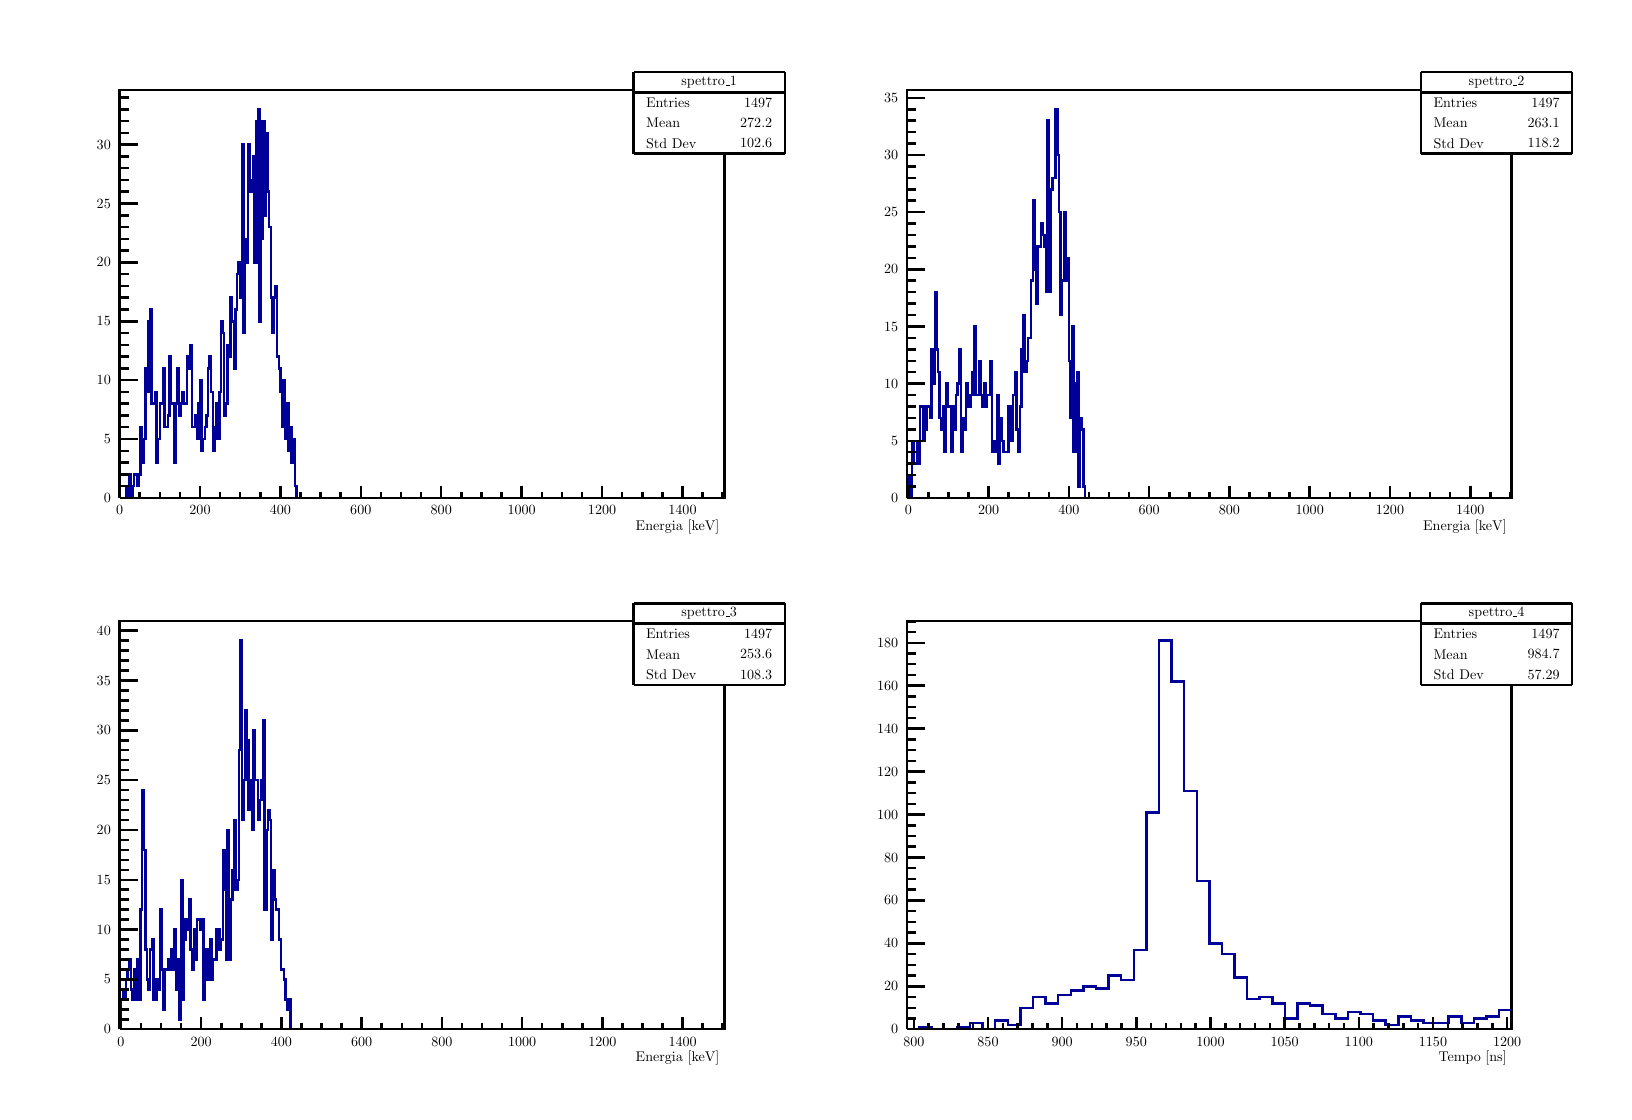
\begin{tikzpicture}
\pgfdeclareplotmark{cross} {
\pgfpathmoveto{\pgfpoint{-0.3\pgfplotmarksize}{\pgfplotmarksize}}
\pgfpathlineto{\pgfpoint{+0.3\pgfplotmarksize}{\pgfplotmarksize}}
\pgfpathlineto{\pgfpoint{+0.3\pgfplotmarksize}{0.3\pgfplotmarksize}}
\pgfpathlineto{\pgfpoint{+1\pgfplotmarksize}{0.3\pgfplotmarksize}}
\pgfpathlineto{\pgfpoint{+1\pgfplotmarksize}{-0.3\pgfplotmarksize}}
\pgfpathlineto{\pgfpoint{+0.3\pgfplotmarksize}{-0.3\pgfplotmarksize}}
\pgfpathlineto{\pgfpoint{+0.3\pgfplotmarksize}{-1.\pgfplotmarksize}}
\pgfpathlineto{\pgfpoint{-0.3\pgfplotmarksize}{-1.\pgfplotmarksize}}
\pgfpathlineto{\pgfpoint{-0.3\pgfplotmarksize}{-0.3\pgfplotmarksize}}
\pgfpathlineto{\pgfpoint{-1.\pgfplotmarksize}{-0.3\pgfplotmarksize}}
\pgfpathlineto{\pgfpoint{-1.\pgfplotmarksize}{0.3\pgfplotmarksize}}
\pgfpathlineto{\pgfpoint{-0.3\pgfplotmarksize}{0.3\pgfplotmarksize}}
\pgfpathclose
\pgfusepathqstroke
}
\pgfdeclareplotmark{cross*} {
\pgfpathmoveto{\pgfpoint{-0.3\pgfplotmarksize}{\pgfplotmarksize}}
\pgfpathlineto{\pgfpoint{+0.3\pgfplotmarksize}{\pgfplotmarksize}}
\pgfpathlineto{\pgfpoint{+0.3\pgfplotmarksize}{0.3\pgfplotmarksize}}
\pgfpathlineto{\pgfpoint{+1\pgfplotmarksize}{0.3\pgfplotmarksize}}
\pgfpathlineto{\pgfpoint{+1\pgfplotmarksize}{-0.3\pgfplotmarksize}}
\pgfpathlineto{\pgfpoint{+0.3\pgfplotmarksize}{-0.3\pgfplotmarksize}}
\pgfpathlineto{\pgfpoint{+0.3\pgfplotmarksize}{-1.\pgfplotmarksize}}
\pgfpathlineto{\pgfpoint{-0.3\pgfplotmarksize}{-1.\pgfplotmarksize}}
\pgfpathlineto{\pgfpoint{-0.3\pgfplotmarksize}{-0.3\pgfplotmarksize}}
\pgfpathlineto{\pgfpoint{-1.\pgfplotmarksize}{-0.3\pgfplotmarksize}}
\pgfpathlineto{\pgfpoint{-1.\pgfplotmarksize}{0.3\pgfplotmarksize}}
\pgfpathlineto{\pgfpoint{-0.3\pgfplotmarksize}{0.3\pgfplotmarksize}}
\pgfpathclose
\pgfusepathqfillstroke
}
\pgfdeclareplotmark{newstar} {
\pgfpathmoveto{\pgfqpoint{0pt}{\pgfplotmarksize}}
\pgfpathlineto{\pgfqpointpolar{44}{0.5\pgfplotmarksize}}
\pgfpathlineto{\pgfqpointpolar{18}{\pgfplotmarksize}}
\pgfpathlineto{\pgfqpointpolar{-20}{0.5\pgfplotmarksize}}
\pgfpathlineto{\pgfqpointpolar{-54}{\pgfplotmarksize}}
\pgfpathlineto{\pgfqpointpolar{-90}{0.5\pgfplotmarksize}}
\pgfpathlineto{\pgfqpointpolar{234}{\pgfplotmarksize}}
\pgfpathlineto{\pgfqpointpolar{198}{0.5\pgfplotmarksize}}
\pgfpathlineto{\pgfqpointpolar{162}{\pgfplotmarksize}}
\pgfpathlineto{\pgfqpointpolar{134}{0.5\pgfplotmarksize}}
\pgfpathclose
\pgfusepathqstroke
}
\pgfdeclareplotmark{newstar*} {
\pgfpathmoveto{\pgfqpoint{0pt}{\pgfplotmarksize}}
\pgfpathlineto{\pgfqpointpolar{44}{0.5\pgfplotmarksize}}
\pgfpathlineto{\pgfqpointpolar{18}{\pgfplotmarksize}}
\pgfpathlineto{\pgfqpointpolar{-20}{0.5\pgfplotmarksize}}
\pgfpathlineto{\pgfqpointpolar{-54}{\pgfplotmarksize}}
\pgfpathlineto{\pgfqpointpolar{-90}{0.5\pgfplotmarksize}}
\pgfpathlineto{\pgfqpointpolar{234}{\pgfplotmarksize}}
\pgfpathlineto{\pgfqpointpolar{198}{0.5\pgfplotmarksize}}
\pgfpathlineto{\pgfqpointpolar{162}{\pgfplotmarksize}}
\pgfpathlineto{\pgfqpointpolar{134}{0.5\pgfplotmarksize}}
\pgfpathclose
\pgfusepathqfillstroke
}
\definecolor{c}{rgb}{1,1,1};
\draw [color=c, fill=c] (0,0) rectangle (20,13.4957);
\draw [color=c, fill=c] (0.2,6.88281) rectangle (9.8,13.3607);
\draw [color=c, fill=c] (1.16,7.5306) rectangle (8.84,12.713);
\definecolor{c}{rgb}{0,0,0};
\draw [c,line width=0.9] (1.16,7.5306) -- (1.16,12.713) -- (8.84,12.713) -- (8.84,7.5306) -- (1.16,7.5306);
\definecolor{c}{rgb}{1,1,1};
\draw [color=c, fill=c] (1.16,7.5306) rectangle (8.84,12.713);
\definecolor{c}{rgb}{0,0,0};
\draw [c,line width=0.9] (1.16,7.5306) -- (1.16,12.713) -- (8.84,12.713) -- (8.84,7.5306) -- (1.16,7.5306);
\definecolor{c}{rgb}{0,0,0.6};
\draw [c,line width=0.9] (1.16,7.5306) -- (1.18043,7.5306) -- (1.18043,7.5306) -- (1.20085,7.5306) -- (1.20085,7.5306) -- (1.22128,7.5306) -- (1.22128,7.5306) -- (1.2417,7.5306) -- (1.2417,7.68016) -- (1.26213,7.68016) -- (1.26213,7.5306) --
 (1.28255,7.5306) -- (1.28255,7.82973) -- (1.30298,7.82973) -- (1.30298,7.5306) -- (1.3234,7.5306) -- (1.3234,7.68016) -- (1.34383,7.68016) -- (1.34383,7.82973) -- (1.36426,7.82973) -- (1.36426,7.82973) -- (1.38468,7.82973) -- (1.38468,7.68016) --
 (1.40511,7.68016) -- (1.40511,7.82973) -- (1.42553,7.82973) -- (1.42553,8.42798) -- (1.44596,8.42798) -- (1.44596,7.97929) -- (1.46638,7.97929) -- (1.46638,8.27842) -- (1.48681,8.27842) -- (1.48681,9.17579) -- (1.50723,9.17579) -- (1.50723,8.87667)
 -- (1.52766,8.87667) -- (1.52766,9.77404) -- (1.54809,9.77404) -- (1.54809,9.92361) -- (1.56851,9.92361) -- (1.56851,8.7271) -- (1.58894,8.7271) -- (1.58894,8.7271) -- (1.60936,8.7271) -- (1.60936,8.87667) -- (1.62979,8.87667) -- (1.62979,7.97929)
 -- (1.65021,7.97929) -- (1.65021,8.27842) -- (1.67064,8.27842) -- (1.67064,8.7271) -- (1.69106,8.7271) -- (1.69106,8.7271) -- (1.71149,8.7271) -- (1.71149,9.17579) -- (1.73191,9.17579) -- (1.73191,8.42798) -- (1.75234,8.42798) -- (1.75234,8.42798)
 -- (1.77277,8.42798) -- (1.77277,8.57754) -- (1.79319,8.57754) -- (1.79319,9.32535) -- (1.81362,9.32535) -- (1.81362,8.7271) -- (1.83404,8.7271) -- (1.83404,8.7271) -- (1.85447,8.7271) -- (1.85447,7.97929) -- (1.87489,7.97929) -- (1.87489,8.7271) --
 (1.89532,8.7271) -- (1.89532,9.17579) -- (1.91574,9.17579) -- (1.91574,8.57754) -- (1.93617,8.57754) -- (1.93617,8.7271) -- (1.9566,8.7271) -- (1.9566,8.87667) -- (1.97702,8.87667) -- (1.97702,8.7271) -- (1.99745,8.7271) -- (1.99745,8.7271) --
 (2.01787,8.7271) -- (2.01787,9.32535) -- (2.0383,9.32535) -- (2.0383,9.17579) -- (2.05872,9.17579) -- (2.05872,9.47492) -- (2.07915,9.47492) -- (2.07915,8.42798) -- (2.09957,8.42798) -- (2.09957,8.42798) -- (2.12,8.42798) -- (2.12,8.57754) --
 (2.14043,8.57754) -- (2.14043,8.27842) -- (2.16085,8.27842) -- (2.16085,8.7271) -- (2.18128,8.7271) -- (2.18128,9.02623) -- (2.2017,9.02623) -- (2.2017,8.12885) -- (2.22213,8.12885) -- (2.22213,8.27842) -- (2.24255,8.27842) -- (2.24255,8.42798) --
 (2.26298,8.42798) -- (2.26298,8.57754) -- (2.2834,8.57754) -- (2.2834,9.17579) -- (2.30383,9.17579) -- (2.30383,9.32535) -- (2.32426,9.32535) -- (2.32426,8.87667) -- (2.34468,8.87667) -- (2.34468,8.12885) -- (2.36511,8.12885) -- (2.36511,8.42798) --
 (2.38553,8.42798) -- (2.38553,8.7271) -- (2.40596,8.7271) -- (2.40596,8.27842) -- (2.42638,8.27842) -- (2.42638,8.87667) -- (2.44681,8.87667) -- (2.44681,9.77404) -- (2.46723,9.77404) -- (2.46723,9.62448) -- (2.48766,9.62448) -- (2.48766,8.57754) --
 (2.50809,8.57754) -- (2.50809,8.7271) -- (2.52851,8.7271) -- (2.52851,9.47492) -- (2.54894,9.47492) -- (2.54894,9.32535) -- (2.56936,9.32535) -- (2.56936,10.0732) -- (2.58979,10.0732) -- (2.58979,9.77404) -- (2.61021,9.77404) -- (2.61021,9.17579) --
 (2.63064,9.17579) -- (2.63064,9.92361) -- (2.65106,9.92361) -- (2.65106,10.3723) -- (2.67149,10.3723) -- (2.67149,10.5219) -- (2.69192,10.5219) -- (2.69192,10.0732) -- (2.71234,10.0732) -- (2.71234,12.0175) -- (2.73277,12.0175) -- (2.73277,9.62448)
 -- (2.75319,9.62448) -- (2.75319,10.821) -- (2.77362,10.821) -- (2.77362,10.5219) -- (2.79404,10.5219) -- (2.79404,12.0175) -- (2.81447,12.0175) -- (2.81447,11.4192) -- (2.83489,11.4192) -- (2.83489,11.5688) -- (2.85532,11.5688) -- (2.85532,11.8679)
 -- (2.87574,11.8679) -- (2.87574,10.5219) -- (2.89617,10.5219) -- (2.89617,12.3166) -- (2.9166,12.3166) -- (2.9166,12.4662) -- (2.93702,12.4662) -- (2.93702,9.77404) -- (2.95745,9.77404) -- (2.95745,10.821) -- (2.97787,10.821) -- (2.97787,12.3166)
 -- (2.9983,12.3166) -- (2.9983,11.1201) -- (3.01872,11.1201) -- (3.01872,12.167) -- (3.03915,12.167) -- (3.03915,11.4192) -- (3.05957,11.4192) -- (3.05957,10.9705) -- (3.08,10.9705) -- (3.08,10.0732) -- (3.10043,10.0732) -- (3.10043,9.62448) --
 (3.12085,9.62448) -- (3.12085,10.0732) -- (3.14128,10.0732) -- (3.14128,10.2227) -- (3.1617,10.2227) -- (3.1617,9.32535) -- (3.18213,9.32535) -- (3.18213,9.17579) -- (3.20255,9.17579) -- (3.20255,8.87667) -- (3.22298,8.87667) -- (3.22298,8.42798) --
 (3.2434,8.42798) -- (3.2434,9.02623) -- (3.26383,9.02623) -- (3.26383,8.27842) -- (3.28426,8.27842) -- (3.28426,8.7271) -- (3.30468,8.7271) -- (3.30468,8.12885) -- (3.32511,8.12885) -- (3.32511,8.42798) -- (3.34553,8.42798) -- (3.34553,7.97929) --
 (3.36596,7.97929) -- (3.36596,8.27842) -- (3.38638,8.27842) -- (3.38638,7.68016) -- (3.40681,7.68016) -- (3.40681,7.5306) -- (3.42723,7.5306) -- (3.42723,7.5306) -- (3.44766,7.5306) -- (3.44766,7.5306) -- (3.46809,7.5306) -- (3.46809,7.5306) --
 (3.48851,7.5306) -- (3.48851,7.5306) -- (3.50894,7.5306) -- (3.50894,7.5306) -- (3.52936,7.5306) -- (3.52936,7.5306) -- (3.54979,7.5306) -- (3.54979,7.5306) -- (3.57021,7.5306) -- (3.57021,7.5306) -- (3.59064,7.5306) -- (3.59064,7.5306) --
 (3.61106,7.5306) -- (3.61106,7.5306) -- (3.63149,7.5306) -- (3.63149,7.5306) -- (3.65191,7.5306) -- (3.65191,7.5306) -- (3.67234,7.5306) -- (3.67234,7.5306) -- (3.69277,7.5306) -- (3.69277,7.5306) -- (3.71319,7.5306) -- (3.71319,7.5306) --
 (3.73362,7.5306) -- (3.73362,7.5306) -- (3.75404,7.5306) -- (3.75404,7.5306) -- (3.77447,7.5306) -- (3.77447,7.5306) -- (3.79489,7.5306) -- (3.79489,7.5306) -- (3.81532,7.5306) -- (3.81532,7.5306) -- (3.83574,7.5306) -- (3.83574,7.5306) --
 (3.85617,7.5306) -- (3.85617,7.5306) -- (3.8766,7.5306) -- (3.8766,7.5306) -- (3.89702,7.5306) -- (3.89702,7.5306) -- (3.91745,7.5306) -- (3.91745,7.5306) -- (3.93787,7.5306) -- (3.93787,7.5306) -- (3.9583,7.5306) -- (3.9583,7.5306) --
 (3.97872,7.5306) -- (3.97872,7.5306) -- (3.99915,7.5306) -- (3.99915,7.5306) -- (4.01957,7.5306) -- (4.01957,7.5306) -- (4.04,7.5306) -- (4.04,7.5306) -- (4.06043,7.5306) -- (4.06043,7.5306) -- (4.08085,7.5306) -- (4.08085,7.5306) --
 (4.10128,7.5306) -- (4.10128,7.5306) -- (4.1217,7.5306) -- (4.1217,7.5306) -- (4.14213,7.5306) -- (4.14213,7.5306) -- (4.16255,7.5306) -- (4.16255,7.5306) -- (4.18298,7.5306) -- (4.18298,7.5306) -- (4.2034,7.5306) -- (4.2034,7.5306) --
 (4.22383,7.5306) -- (4.22383,7.5306) -- (4.24426,7.5306) -- (4.24426,7.5306) -- (4.26468,7.5306) -- (4.26468,7.5306) -- (4.28511,7.5306) -- (4.28511,7.5306) -- (4.30553,7.5306) -- (4.30553,7.5306) -- (4.32596,7.5306) -- (4.32596,7.5306) --
 (4.34638,7.5306) -- (4.34638,7.5306) -- (4.36681,7.5306) -- (4.36681,7.5306) -- (4.38723,7.5306) -- (4.38723,7.5306) -- (4.40766,7.5306) -- (4.40766,7.5306) -- (4.42809,7.5306) -- (4.42809,7.5306) -- (4.44851,7.5306) -- (4.44851,7.5306) --
 (4.46894,7.5306) -- (4.46894,7.5306) -- (4.48936,7.5306) -- (4.48936,7.5306) -- (4.50979,7.5306) -- (4.50979,7.5306) -- (4.53021,7.5306) -- (4.53021,7.5306) -- (4.55064,7.5306) -- (4.55064,7.5306) -- (4.57106,7.5306) -- (4.57106,7.5306) --
 (4.59149,7.5306) -- (4.59149,7.5306) -- (4.61192,7.5306) -- (4.61192,7.5306) -- (4.63234,7.5306) -- (4.63234,7.5306) -- (4.65277,7.5306) -- (4.65277,7.5306) -- (4.67319,7.5306) -- (4.67319,7.5306) -- (4.69362,7.5306) -- (4.69362,7.5306) --
 (4.71404,7.5306) -- (4.71404,7.5306) -- (4.73447,7.5306) -- (4.73447,7.5306) -- (4.75489,7.5306) -- (4.75489,7.5306) -- (4.77532,7.5306) -- (4.77532,7.5306) -- (4.79574,7.5306) -- (4.79574,7.5306) -- (4.81617,7.5306) -- (4.81617,7.5306) --
 (4.8366,7.5306) -- (4.8366,7.5306) -- (4.85702,7.5306) -- (4.85702,7.5306) -- (4.87745,7.5306) -- (4.87745,7.5306) -- (4.89787,7.5306) -- (4.89787,7.5306) -- (4.9183,7.5306) -- (4.9183,7.5306) -- (4.93872,7.5306) -- (4.93872,7.5306) --
 (4.95915,7.5306) -- (4.95915,7.5306) -- (4.97957,7.5306) -- (4.97957,7.5306) -- (5,7.5306) -- (5,7.5306) -- (5.02043,7.5306) -- (5.02043,7.5306) -- (5.04085,7.5306) -- (5.04085,7.5306) -- (5.06128,7.5306) -- (5.06128,7.5306) -- (5.0817,7.5306) --
 (5.0817,7.5306) -- (5.10213,7.5306) -- (5.10213,7.5306) -- (5.12255,7.5306) -- (5.12255,7.5306) -- (5.14298,7.5306) -- (5.14298,7.5306) -- (5.1634,7.5306) -- (5.1634,7.5306) -- (5.18383,7.5306) -- (5.18383,7.5306) -- (5.20426,7.5306) --
 (5.20426,7.5306) -- (5.22468,7.5306) -- (5.22468,7.5306) -- (5.24511,7.5306) -- (5.24511,7.5306) -- (5.26553,7.5306) -- (5.26553,7.5306) -- (5.28596,7.5306) -- (5.28596,7.5306) -- (5.30638,7.5306) -- (5.30638,7.5306) -- (5.32681,7.5306) --
 (5.32681,7.5306) -- (5.34723,7.5306) -- (5.34723,7.5306) -- (5.36766,7.5306) -- (5.36766,7.5306) -- (5.38808,7.5306) -- (5.38808,7.5306) -- (5.40851,7.5306) -- (5.40851,7.5306) -- (5.42894,7.5306) -- (5.42894,7.5306) -- (5.44936,7.5306) --
 (5.44936,7.5306) -- (5.46979,7.5306) -- (5.46979,7.5306) -- (5.49021,7.5306) -- (5.49021,7.5306) -- (5.51064,7.5306) -- (5.51064,7.5306) -- (5.53106,7.5306) -- (5.53106,7.5306) -- (5.55149,7.5306) -- (5.55149,7.5306) -- (5.57191,7.5306) --
 (5.57191,7.5306) -- (5.59234,7.5306) -- (5.59234,7.5306) -- (5.61277,7.5306) -- (5.61277,7.5306) -- (5.63319,7.5306) -- (5.63319,7.5306) -- (5.65362,7.5306) -- (5.65362,7.5306) -- (5.67404,7.5306) -- (5.67404,7.5306) -- (5.69447,7.5306) --
 (5.69447,7.5306) -- (5.71489,7.5306) -- (5.71489,7.5306) -- (5.73532,7.5306) -- (5.73532,7.5306) -- (5.75574,7.5306) -- (5.75574,7.5306) -- (5.77617,7.5306) -- (5.77617,7.5306) -- (5.7966,7.5306) -- (5.7966,7.5306) -- (5.81702,7.5306) --
 (5.81702,7.5306) -- (5.83745,7.5306) -- (5.83745,7.5306) -- (5.85787,7.5306) -- (5.85787,7.5306) -- (5.8783,7.5306) -- (5.8783,7.5306) -- (5.89872,7.5306) -- (5.89872,7.5306) -- (5.91915,7.5306) -- (5.91915,7.5306) -- (5.93957,7.5306) --
 (5.93957,7.5306) -- (5.96,7.5306) -- (5.96,7.5306) -- (5.98043,7.5306) -- (5.98043,7.5306) -- (6.00085,7.5306) -- (6.00085,7.5306) -- (6.02128,7.5306) -- (6.02128,7.5306) -- (6.0417,7.5306) -- (6.0417,7.5306) -- (6.06213,7.5306) -- (6.06213,7.5306)
 -- (6.08255,7.5306) -- (6.08255,7.5306) -- (6.10298,7.5306) -- (6.10298,7.5306) -- (6.1234,7.5306) -- (6.1234,7.5306) -- (6.14383,7.5306) -- (6.14383,7.5306) -- (6.16426,7.5306) -- (6.16426,7.5306) -- (6.18468,7.5306) -- (6.18468,7.5306) --
 (6.20511,7.5306) -- (6.20511,7.5306) -- (6.22553,7.5306) -- (6.22553,7.5306) -- (6.24596,7.5306) -- (6.24596,7.5306) -- (6.26638,7.5306) -- (6.26638,7.5306) -- (6.28681,7.5306) -- (6.28681,7.5306) -- (6.30723,7.5306) -- (6.30723,7.5306) --
 (6.32766,7.5306) -- (6.32766,7.5306) -- (6.34808,7.5306) -- (6.34808,7.5306) -- (6.36851,7.5306) -- (6.36851,7.5306) -- (6.38894,7.5306) -- (6.38894,7.5306) -- (6.40936,7.5306) -- (6.40936,7.5306) -- (6.42979,7.5306) -- (6.42979,7.5306) --
 (6.45021,7.5306) -- (6.45021,7.5306) -- (6.47064,7.5306) -- (6.47064,7.5306) -- (6.49106,7.5306) -- (6.49106,7.5306) -- (6.51149,7.5306) -- (6.51149,7.5306) -- (6.53191,7.5306) -- (6.53191,7.5306) -- (6.55234,7.5306) -- (6.55234,7.5306) --
 (6.57277,7.5306) -- (6.57277,7.5306) -- (6.59319,7.5306) -- (6.59319,7.5306) -- (6.61362,7.5306) -- (6.61362,7.5306) -- (6.63404,7.5306) -- (6.63404,7.5306) -- (6.65447,7.5306) -- (6.65447,7.5306) -- (6.67489,7.5306) -- (6.67489,7.5306) --
 (6.69532,7.5306) -- (6.69532,7.5306) -- (6.71574,7.5306) -- (6.71574,7.5306) -- (6.73617,7.5306) -- (6.73617,7.5306) -- (6.7566,7.5306) -- (6.7566,7.5306) -- (6.77702,7.5306) -- (6.77702,7.5306) -- (6.79745,7.5306) -- (6.79745,7.5306) --
 (6.81787,7.5306) -- (6.81787,7.5306) -- (6.8383,7.5306) -- (6.8383,7.5306) -- (6.85872,7.5306) -- (6.85872,7.5306) -- (6.87915,7.5306) -- (6.87915,7.5306) -- (6.89957,7.5306) -- (6.89957,7.5306) -- (6.92,7.5306) -- (6.92,7.5306) -- (6.94043,7.5306)
 -- (6.94043,7.5306) -- (6.96085,7.5306) -- (6.96085,7.5306) -- (6.98128,7.5306) -- (6.98128,7.5306) -- (7.0017,7.5306) -- (7.0017,7.5306) -- (7.02213,7.5306) -- (7.02213,7.5306) -- (7.04255,7.5306) -- (7.04255,7.5306) -- (7.06298,7.5306) --
 (7.06298,7.5306) -- (7.0834,7.5306) -- (7.0834,7.5306) -- (7.10383,7.5306) -- (7.10383,7.5306) -- (7.12426,7.5306) -- (7.12426,7.5306) -- (7.14468,7.5306) -- (7.14468,7.5306) -- (7.16511,7.5306) -- (7.16511,7.5306) -- (7.18553,7.5306) --
 (7.18553,7.5306) -- (7.20596,7.5306) -- (7.20596,7.5306) -- (7.22638,7.5306) -- (7.22638,7.5306) -- (7.24681,7.5306) -- (7.24681,7.5306) -- (7.26723,7.5306) -- (7.26723,7.5306) -- (7.28766,7.5306) -- (7.28766,7.5306) -- (7.30808,7.5306) --
 (7.30808,7.5306) -- (7.32851,7.5306) -- (7.32851,7.5306) -- (7.34894,7.5306) -- (7.34894,7.5306) -- (7.36936,7.5306) -- (7.36936,7.5306) -- (7.38979,7.5306) -- (7.38979,7.5306) -- (7.41021,7.5306) -- (7.41021,7.5306) -- (7.43064,7.5306) --
 (7.43064,7.5306) -- (7.45106,7.5306) -- (7.45106,7.5306) -- (7.47149,7.5306) -- (7.47149,7.5306) -- (7.49191,7.5306) -- (7.49191,7.5306) -- (7.51234,7.5306) -- (7.51234,7.5306) -- (7.53277,7.5306) -- (7.53277,7.5306) -- (7.55319,7.5306) --
 (7.55319,7.5306) -- (7.57362,7.5306) -- (7.57362,7.5306) -- (7.59404,7.5306) -- (7.59404,7.5306) -- (7.61447,7.5306) -- (7.61447,7.5306) -- (7.63489,7.5306) -- (7.63489,7.5306) -- (7.65532,7.5306) -- (7.65532,7.5306) -- (7.67574,7.5306) --
 (7.67574,7.5306) -- (7.69617,7.5306) -- (7.69617,7.5306) -- (7.7166,7.5306) -- (7.7166,7.5306) -- (7.73702,7.5306) -- (7.73702,7.5306) -- (7.75745,7.5306) -- (7.75745,7.5306) -- (7.77787,7.5306) -- (7.77787,7.5306) -- (7.7983,7.5306) --
 (7.7983,7.5306) -- (7.81872,7.5306) -- (7.81872,7.5306) -- (7.83915,7.5306) -- (7.83915,7.5306) -- (7.85957,7.5306) -- (7.85957,7.5306) -- (7.88,7.5306) -- (7.88,7.5306) -- (7.90043,7.5306) -- (7.90043,7.5306) -- (7.92085,7.5306) -- (7.92085,7.5306)
 -- (7.94128,7.5306) -- (7.94128,7.5306) -- (7.9617,7.5306) -- (7.9617,7.5306) -- (7.98213,7.5306) -- (7.98213,7.5306) -- (8.00255,7.5306) -- (8.00255,7.5306) -- (8.02298,7.5306) -- (8.02298,7.5306) -- (8.0434,7.5306) -- (8.0434,7.5306) --
 (8.06383,7.5306) -- (8.06383,7.5306) -- (8.08426,7.5306) -- (8.08426,7.5306) -- (8.10468,7.5306) -- (8.10468,7.5306) -- (8.12511,7.5306) -- (8.12511,7.5306) -- (8.14553,7.5306) -- (8.14553,7.5306) -- (8.16596,7.5306) -- (8.16596,7.5306) --
 (8.18638,7.5306) -- (8.18638,7.5306) -- (8.20681,7.5306) -- (8.20681,7.5306) -- (8.22723,7.5306) -- (8.22723,7.5306) -- (8.24766,7.5306) -- (8.24766,7.5306) -- (8.26809,7.5306) -- (8.26809,7.5306) -- (8.28851,7.5306) -- (8.28851,7.5306) --
 (8.30894,7.5306) -- (8.30894,7.5306) -- (8.32936,7.5306) -- (8.32936,7.5306) -- (8.34979,7.5306) -- (8.34979,7.5306) -- (8.37021,7.5306) -- (8.37021,7.5306) -- (8.39064,7.5306) -- (8.39064,7.5306) -- (8.41106,7.5306) -- (8.41106,7.5306) --
 (8.43149,7.5306) -- (8.43149,7.5306) -- (8.45191,7.5306) -- (8.45191,7.5306) -- (8.47234,7.5306) -- (8.47234,7.5306) -- (8.49277,7.5306) -- (8.49277,7.5306) -- (8.51319,7.5306) -- (8.51319,7.5306) -- (8.53362,7.5306) -- (8.53362,7.5306) --
 (8.55404,7.5306) -- (8.55404,7.5306) -- (8.57447,7.5306) -- (8.57447,7.5306) -- (8.59489,7.5306) -- (8.59489,7.5306) -- (8.61532,7.5306) -- (8.61532,7.5306) -- (8.63575,7.5306) -- (8.63575,7.5306) -- (8.65617,7.5306) -- (8.65617,7.5306) --
 (8.6766,7.5306) -- (8.6766,7.5306) -- (8.69702,7.5306) -- (8.69702,7.5306) -- (8.71745,7.5306) -- (8.71745,7.5306) -- (8.73787,7.5306) -- (8.73787,7.5306) -- (8.7583,7.5306) -- (8.7583,7.5306) -- (8.77872,7.5306) -- (8.77872,7.5306) --
 (8.79915,7.5306) -- (8.79915,7.5306) -- (8.81957,7.5306) -- (8.81957,7.5306) -- (8.84,7.5306);
\definecolor{c}{rgb}{1,1,1};
\draw [color=c, fill=c] (7.688,11.9032) rectangle (9.608,12.9397);
\definecolor{c}{rgb}{0,0,0};
\draw [c,line width=0.9] (7.688,11.9032) -- (9.608,11.9032);
\draw [c,line width=0.9] (9.608,11.9032) -- (9.608,12.9397);
\draw [c,line width=0.9] (9.608,12.9397) -- (7.688,12.9397);
\draw [c,line width=0.9] (7.688,12.9397) -- (7.688,11.9032);
\draw (8.648,12.8101) node[scale=0.509285, color=c, rotate=0]{spettro\_1};
\draw [c,line width=0.9] (7.688,12.6806) -- (9.608,12.6806);
\draw [anchor= west] (7.784,12.551) node[scale=0.509285, color=c, rotate=0]{Entries };
\draw [anchor= east] (9.512,12.551) node[scale=0.509285, color=c, rotate=0]{ 1497};
\draw [anchor= west] (7.784,12.2919) node[scale=0.509285, color=c, rotate=0]{Mean  };
\draw [anchor= east] (9.512,12.2919) node[scale=0.509285, color=c, rotate=0]{  272.2};
\draw [anchor= west] (7.784,12.0328) node[scale=0.509285, color=c, rotate=0]{Std Dev   };
\draw [anchor= east] (9.512,12.0328) node[scale=0.509285, color=c, rotate=0]{  102.6};
\draw [c,line width=0.9] (1.16,7.5306) -- (8.84,7.5306);
\draw [anchor= east] (8.84,7.16784) node[scale=0.509285, color=c, rotate=0]{Energia [keV]};
\draw [c,line width=0.9] (1.1601,7.68607) -- (1.1601,7.5306);
\draw [c,line width=0.9] (1.41542,7.60834) -- (1.41542,7.5306);
\draw [c,line width=0.9] (1.67074,7.60834) -- (1.67074,7.5306);
\draw [c,line width=0.9] (1.92606,7.60834) -- (1.92606,7.5306);
\draw [c,line width=0.9] (2.18138,7.68607) -- (2.18138,7.5306);
\draw [c,line width=0.9] (2.4367,7.60834) -- (2.4367,7.5306);
\draw [c,line width=0.9] (2.69202,7.60834) -- (2.69202,7.5306);
\draw [c,line width=0.9] (2.94734,7.60834) -- (2.94734,7.5306);
\draw [c,line width=0.9] (3.20266,7.68607) -- (3.20266,7.5306);
\draw [c,line width=0.9] (3.45798,7.60834) -- (3.45798,7.5306);
\draw [c,line width=0.9] (3.7133,7.60834) -- (3.7133,7.5306);
\draw [c,line width=0.9] (3.96862,7.60834) -- (3.96862,7.5306);
\draw [c,line width=0.9] (4.22394,7.68607) -- (4.22394,7.5306);
\draw [c,line width=0.9] (4.47925,7.60834) -- (4.47925,7.5306);
\draw [c,line width=0.9] (4.73457,7.60834) -- (4.73457,7.5306);
\draw [c,line width=0.9] (4.98989,7.60834) -- (4.98989,7.5306);
\draw [c,line width=0.9] (5.24521,7.68607) -- (5.24521,7.5306);
\draw [c,line width=0.9] (5.50053,7.60834) -- (5.50053,7.5306);
\draw [c,line width=0.9] (5.75585,7.60834) -- (5.75585,7.5306);
\draw [c,line width=0.9] (6.01117,7.60834) -- (6.01117,7.5306);
\draw [c,line width=0.9] (6.26649,7.68607) -- (6.26649,7.5306);
\draw [c,line width=0.9] (6.52181,7.60834) -- (6.52181,7.5306);
\draw [c,line width=0.9] (6.77713,7.60834) -- (6.77713,7.5306);
\draw [c,line width=0.9] (7.03245,7.60834) -- (7.03245,7.5306);
\draw [c,line width=0.9] (7.28777,7.68607) -- (7.28777,7.5306);
\draw [c,line width=0.9] (7.54309,7.60834) -- (7.54309,7.5306);
\draw [c,line width=0.9] (7.79841,7.60834) -- (7.79841,7.5306);
\draw [c,line width=0.9] (8.05373,7.60834) -- (8.05373,7.5306);
\draw [c,line width=0.9] (8.30905,7.68607) -- (8.30905,7.5306);
\draw [c,line width=0.9] (1.1601,7.68607) -- (1.1601,7.5306);
\draw [c,line width=0.9] (8.30905,7.68607) -- (8.30905,7.5306);
\draw [c,line width=0.9] (8.56436,7.60834) -- (8.56436,7.5306);
\draw [c,line width=0.9] (8.81968,7.60834) -- (8.81968,7.5306);
\draw [anchor=base] (1.1601,7.31683) node[scale=0.509285, color=c, rotate=0]{0};
\draw [anchor=base] (2.18138,7.31683) node[scale=0.509285, color=c, rotate=0]{200};
\draw [anchor=base] (3.20266,7.31683) node[scale=0.509285, color=c, rotate=0]{400};
\draw [anchor=base] (4.22394,7.31683) node[scale=0.509285, color=c, rotate=0]{600};
\draw [anchor=base] (5.24521,7.31683) node[scale=0.509285, color=c, rotate=0]{800};
\draw [anchor=base] (6.26649,7.31683) node[scale=0.509285, color=c, rotate=0]{1000};
\draw [anchor=base] (7.28777,7.31683) node[scale=0.509285, color=c, rotate=0]{1200};
\draw [anchor=base] (8.30905,7.31683) node[scale=0.509285, color=c, rotate=0]{1400};
\draw [c,line width=0.9] (1.16,7.5306) -- (1.16,12.713);
\draw [c,line width=0.9] (1.3904,7.5306) -- (1.16,7.5306);
\draw [c,line width=0.9] (1.2752,7.68016) -- (1.16,7.68016);
\draw [c,line width=0.9] (1.2752,7.82973) -- (1.16,7.82973);
\draw [c,line width=0.9] (1.2752,7.97929) -- (1.16,7.97929);
\draw [c,line width=0.9] (1.2752,8.12885) -- (1.16,8.12885);
\draw [c,line width=0.9] (1.3904,8.27842) -- (1.16,8.27842);
\draw [c,line width=0.9] (1.2752,8.42798) -- (1.16,8.42798);
\draw [c,line width=0.9] (1.2752,8.57754) -- (1.16,8.57754);
\draw [c,line width=0.9] (1.2752,8.7271) -- (1.16,8.7271);
\draw [c,line width=0.9] (1.2752,8.87667) -- (1.16,8.87667);
\draw [c,line width=0.9] (1.3904,9.02623) -- (1.16,9.02623);
\draw [c,line width=0.9] (1.2752,9.17579) -- (1.16,9.17579);
\draw [c,line width=0.9] (1.2752,9.32535) -- (1.16,9.32535);
\draw [c,line width=0.9] (1.2752,9.47492) -- (1.16,9.47492);
\draw [c,line width=0.9] (1.2752,9.62448) -- (1.16,9.62448);
\draw [c,line width=0.9] (1.3904,9.77404) -- (1.16,9.77404);
\draw [c,line width=0.9] (1.2752,9.92361) -- (1.16,9.92361);
\draw [c,line width=0.9] (1.2752,10.0732) -- (1.16,10.0732);
\draw [c,line width=0.9] (1.2752,10.2227) -- (1.16,10.2227);
\draw [c,line width=0.9] (1.2752,10.3723) -- (1.16,10.3723);
\draw [c,line width=0.9] (1.3904,10.5219) -- (1.16,10.5219);
\draw [c,line width=0.9] (1.2752,10.6714) -- (1.16,10.6714);
\draw [c,line width=0.9] (1.2752,10.821) -- (1.16,10.821);
\draw [c,line width=0.9] (1.2752,10.9705) -- (1.16,10.9705);
\draw [c,line width=0.9] (1.2752,11.1201) -- (1.16,11.1201);
\draw [c,line width=0.9] (1.3904,11.2697) -- (1.16,11.2697);
\draw [c,line width=0.9] (1.2752,11.4192) -- (1.16,11.4192);
\draw [c,line width=0.9] (1.2752,11.5688) -- (1.16,11.5688);
\draw [c,line width=0.9] (1.2752,11.7184) -- (1.16,11.7184);
\draw [c,line width=0.9] (1.2752,11.8679) -- (1.16,11.8679);
\draw [c,line width=0.9] (1.3904,12.0175) -- (1.16,12.0175);
\draw [c,line width=0.9] (1.3904,12.0175) -- (1.16,12.0175);
\draw [c,line width=0.9] (1.2752,12.167) -- (1.16,12.167);
\draw [c,line width=0.9] (1.2752,12.3166) -- (1.16,12.3166);
\draw [c,line width=0.9] (1.2752,12.4662) -- (1.16,12.4662);
\draw [c,line width=0.9] (1.2752,12.6157) -- (1.16,12.6157);
\draw [anchor= east] (1.112,7.5306) node[scale=0.509285, color=c, rotate=0]{0};
\draw [anchor= east] (1.112,8.27842) node[scale=0.509285, color=c, rotate=0]{5};
\draw [anchor= east] (1.112,9.02623) node[scale=0.509285, color=c, rotate=0]{10};
\draw [anchor= east] (1.112,9.77404) node[scale=0.509285, color=c, rotate=0]{15};
\draw [anchor= east] (1.112,10.5219) node[scale=0.509285, color=c, rotate=0]{20};
\draw [anchor= east] (1.112,11.2697) node[scale=0.509285, color=c, rotate=0]{25};
\draw [anchor= east] (1.112,12.0175) node[scale=0.509285, color=c, rotate=0]{30};
\definecolor{c}{rgb}{1,1,1};
\draw [color=c, fill=c] (7.688,11.9032) rectangle (9.608,12.9397);
\definecolor{c}{rgb}{0,0,0};
\draw [c,line width=0.9] (7.688,11.9032) -- (9.608,11.9032);
\draw [c,line width=0.9] (9.608,11.9032) -- (9.608,12.9397);
\draw [c,line width=0.9] (9.608,12.9397) -- (7.688,12.9397);
\draw [c,line width=0.9] (7.688,12.9397) -- (7.688,11.9032);
\draw (8.648,12.8101) node[scale=0.509285, color=c, rotate=0]{spettro\_1};
\draw [c,line width=0.9] (7.688,12.6806) -- (9.608,12.6806);
\draw [anchor= west] (7.784,12.551) node[scale=0.509285, color=c, rotate=0]{Entries };
\draw [anchor= east] (9.512,12.551) node[scale=0.509285, color=c, rotate=0]{ 1497};
\draw [anchor= west] (7.784,12.2919) node[scale=0.509285, color=c, rotate=0]{Mean  };
\draw [anchor= east] (9.512,12.2919) node[scale=0.509285, color=c, rotate=0]{  272.2};
\draw [anchor= west] (7.784,12.0328) node[scale=0.509285, color=c, rotate=0]{Std Dev   };
\draw [anchor= east] (9.512,12.0328) node[scale=0.509285, color=c, rotate=0]{  102.6};
\definecolor{c}{rgb}{1,1,1};
\draw [color=c, fill=c] (10.2,6.88281) rectangle (19.8,13.3607);
\draw [color=c, fill=c] (11.16,7.5306) rectangle (18.84,12.713);
\definecolor{c}{rgb}{0,0,0};
\draw [c,line width=0.9] (11.16,7.5306) -- (11.16,12.713) -- (18.84,12.713) -- (18.84,7.5306) -- (11.16,7.5306);
\definecolor{c}{rgb}{1,1,1};
\draw [color=c, fill=c] (11.16,7.5306) rectangle (18.84,12.713);
\definecolor{c}{rgb}{0,0,0};
\draw [c,line width=0.9] (11.16,7.5306) -- (11.16,12.713) -- (18.84,12.713) -- (18.84,7.5306) -- (11.16,7.5306);
\definecolor{c}{rgb}{0,0,0.6};
\draw [c,line width=0.9] (11.16,7.67577) -- (11.1808,7.67577) -- (11.1808,7.82093) -- (11.2015,7.82093) -- (11.2015,7.5306) -- (11.2223,7.5306) -- (11.2223,8.25642) -- (11.243,8.25642) -- (11.243,7.96609) -- (11.2638,7.96609) -- (11.2638,7.96609) --
 (11.2845,7.96609) -- (11.2845,8.25642) -- (11.3053,8.25642) -- (11.3053,7.96609) -- (11.3261,7.96609) -- (11.3261,8.69191) -- (11.3468,8.69191) -- (11.3468,8.69191) -- (11.3676,8.69191) -- (11.3676,8.25642) -- (11.3883,8.25642) -- (11.3883,8.40158)
 -- (11.4091,8.40158) -- (11.4091,8.69191) -- (11.4298,8.69191) -- (11.4298,8.69191) -- (11.4506,8.69191) -- (11.4506,8.54675) -- (11.4714,8.54675) -- (11.4714,9.41773) -- (11.4921,9.41773) -- (11.4921,8.98224) -- (11.5129,8.98224) --
 (11.5129,10.1436) -- (11.5336,10.1436) -- (11.5336,9.41773) -- (11.5544,9.41773) -- (11.5544,9.1274) -- (11.5751,9.1274) -- (11.5751,8.54675) -- (11.5959,8.54675) -- (11.5959,8.40158) -- (11.6166,8.40158) -- (11.6166,8.69191) -- (11.6374,8.69191) --
 (11.6374,8.11126) -- (11.6582,8.11126) -- (11.6582,8.98224) -- (11.6789,8.98224) -- (11.6789,8.69191) -- (11.6997,8.69191) -- (11.6997,8.69191) -- (11.7204,8.69191) -- (11.7204,8.11126) -- (11.7412,8.11126) -- (11.7412,8.69191) -- (11.7619,8.69191)
 -- (11.7619,8.40158) -- (11.7827,8.40158) -- (11.7827,8.83708) -- (11.8035,8.83708) -- (11.8035,8.98224) -- (11.8242,8.98224) -- (11.8242,9.41773) -- (11.845,9.41773) -- (11.845,8.11126) -- (11.8657,8.11126) -- (11.8657,8.54675) -- (11.8865,8.54675)
 -- (11.8865,8.40158) -- (11.9072,8.40158) -- (11.9072,8.98224) -- (11.928,8.98224) -- (11.928,8.69191) -- (11.9488,8.69191) -- (11.9488,8.69191) -- (11.9695,8.69191) -- (11.9695,8.83708) -- (11.9903,8.83708) -- (11.9903,9.1274) -- (12.011,9.1274) --
 (12.011,9.70806) -- (12.0318,9.70806) -- (12.0318,8.83708) -- (12.0525,8.83708) -- (12.0525,8.83708) -- (12.0733,8.83708) -- (12.0733,9.27257) -- (12.0941,9.27257) -- (12.0941,8.83708) -- (12.1148,8.83708) -- (12.1148,8.69191) -- (12.1356,8.69191)
 -- (12.1356,8.98224) -- (12.1563,8.98224) -- (12.1563,8.69191) -- (12.1771,8.69191) -- (12.1771,8.83708) -- (12.1978,8.83708) -- (12.1978,8.83708) -- (12.2186,8.83708) -- (12.2186,9.27257) -- (12.2394,9.27257) -- (12.2394,8.11126) --
 (12.2601,8.11126) -- (12.2601,8.25642) -- (12.2809,8.25642) -- (12.2809,8.11126) -- (12.3016,8.11126) -- (12.3016,8.83708) -- (12.3224,8.83708) -- (12.3224,7.96609) -- (12.3431,7.96609) -- (12.3431,8.54675) -- (12.3639,8.54675) -- (12.3639,8.25642)
 -- (12.3846,8.25642) -- (12.3846,8.11126) -- (12.4054,8.11126) -- (12.4054,8.11126) -- (12.4262,8.11126) -- (12.4262,8.11126) -- (12.4469,8.11126) -- (12.4469,8.69191) -- (12.4677,8.69191) -- (12.4677,8.69191) -- (12.4884,8.69191) --
 (12.4884,8.25642) -- (12.5092,8.25642) -- (12.5092,8.83708) -- (12.5299,8.83708) -- (12.5299,9.1274) -- (12.5507,9.1274) -- (12.5507,8.40158) -- (12.5715,8.40158) -- (12.5715,8.11126) -- (12.5922,8.11126) -- (12.5922,8.69191) -- (12.613,8.69191) --
 (12.613,9.41773) -- (12.6337,9.41773) -- (12.6337,9.85322) -- (12.6545,9.85322) -- (12.6545,9.1274) -- (12.6752,9.1274) -- (12.6752,9.27257) -- (12.696,9.27257) -- (12.696,9.5629) -- (12.7168,9.5629) -- (12.7168,9.5629) -- (12.7375,9.5629) --
 (12.7375,10.2887) -- (12.7583,10.2887) -- (12.7583,11.3049) -- (12.779,11.3049) -- (12.779,10.4339) -- (12.7998,10.4339) -- (12.7998,9.99839) -- (12.8205,9.99839) -- (12.8205,10.7242) -- (12.8413,10.7242) -- (12.8413,10.7242) -- (12.8621,10.7242) --
 (12.8621,11.0145) -- (12.8828,11.0145) -- (12.8828,10.8694) -- (12.9036,10.8694) -- (12.9036,10.7242) -- (12.9243,10.7242) -- (12.9243,10.1436) -- (12.9451,10.1436) -- (12.9451,12.321) -- (12.9658,12.321) -- (12.9658,10.1436) -- (12.9866,10.1436) --
 (12.9866,11.45) -- (13.0074,11.45) -- (13.0074,11.5952) -- (13.0281,11.5952) -- (13.0281,11.5952) -- (13.0489,11.5952) -- (13.0489,12.4662) -- (13.0696,12.4662) -- (13.0696,11.8855) -- (13.0904,11.8855) -- (13.0904,11.1597) -- (13.1111,11.1597) --
 (13.1111,9.85322) -- (13.1319,9.85322) -- (13.1319,10.2887) -- (13.1526,10.2887) -- (13.1526,11.1597) -- (13.1734,11.1597) -- (13.1734,10.2887) -- (13.1942,10.2887) -- (13.1942,10.579) -- (13.2149,10.579) -- (13.2149,9.27257) -- (13.2357,9.27257) --
 (13.2357,8.54675) -- (13.2564,8.54675) -- (13.2564,9.70806) -- (13.2772,9.70806) -- (13.2772,8.11126) -- (13.2979,8.11126) -- (13.2979,8.98224) -- (13.3187,8.98224) -- (13.3187,9.1274) -- (13.3395,9.1274) -- (13.3395,7.67577) -- (13.3602,7.67577) --
 (13.3602,8.54675) -- (13.381,8.54675) -- (13.381,8.40158) -- (13.4017,8.40158) -- (13.4017,7.67577) -- (13.4225,7.67577) -- (13.4225,7.5306) -- (13.4432,7.5306) -- (13.4432,7.5306) -- (13.464,7.5306) -- (13.464,7.5306) -- (13.4848,7.5306) --
 (13.4848,7.5306) -- (13.5055,7.5306) -- (13.5055,7.5306) -- (13.5263,7.5306) -- (13.5263,7.5306) -- (13.547,7.5306) -- (13.547,7.5306) -- (13.5678,7.5306) -- (13.5678,7.5306) -- (13.5885,7.5306) -- (13.5885,7.5306) -- (13.6093,7.5306) --
 (13.6093,7.5306) -- (13.6301,7.5306) -- (13.6301,7.5306) -- (13.6508,7.5306) -- (13.6508,7.5306) -- (13.6716,7.5306) -- (13.6716,7.5306) -- (13.6923,7.5306) -- (13.6923,7.5306) -- (13.7131,7.5306) -- (13.7131,7.5306) -- (13.7338,7.5306) --
 (13.7338,7.5306) -- (13.7546,7.5306) -- (13.7546,7.5306) -- (13.7754,7.5306) -- (13.7754,7.5306) -- (13.7961,7.5306) -- (13.7961,7.5306) -- (13.8169,7.5306) -- (13.8169,7.5306) -- (13.8376,7.5306) -- (13.8376,7.5306) -- (13.8584,7.5306) --
 (13.8584,7.5306) -- (13.8791,7.5306) -- (13.8791,7.5306) -- (13.8999,7.5306) -- (13.8999,7.5306) -- (13.9206,7.5306) -- (13.9206,7.5306) -- (13.9414,7.5306) -- (13.9414,7.5306) -- (13.9622,7.5306) -- (13.9622,7.5306) -- (13.9829,7.5306) --
 (13.9829,7.5306) -- (14.0037,7.5306) -- (14.0037,7.5306) -- (14.0244,7.5306) -- (14.0244,7.5306) -- (14.0452,7.5306) -- (14.0452,7.5306) -- (14.0659,7.5306) -- (14.0659,7.5306) -- (14.0867,7.5306) -- (14.0867,7.5306) -- (14.1075,7.5306) --
 (14.1075,7.5306) -- (14.1282,7.5306) -- (14.1282,7.5306) -- (14.149,7.5306) -- (14.149,7.5306) -- (14.1697,7.5306) -- (14.1697,7.5306) -- (14.1905,7.5306) -- (14.1905,7.5306) -- (14.2112,7.5306) -- (14.2112,7.5306) -- (14.232,7.5306) --
 (14.232,7.5306) -- (14.2528,7.5306) -- (14.2528,7.5306) -- (14.2735,7.5306) -- (14.2735,7.5306) -- (14.2943,7.5306) -- (14.2943,7.5306) -- (14.315,7.5306) -- (14.315,7.5306) -- (14.3358,7.5306) -- (14.3358,7.5306) -- (14.3565,7.5306) --
 (14.3565,7.5306) -- (14.3773,7.5306) -- (14.3773,7.5306) -- (14.3981,7.5306) -- (14.3981,7.5306) -- (14.4188,7.5306) -- (14.4188,7.5306) -- (14.4396,7.5306) -- (14.4396,7.5306) -- (14.4603,7.5306) -- (14.4603,7.5306) -- (14.4811,7.5306) --
 (14.4811,7.5306) -- (14.5018,7.5306) -- (14.5018,7.5306) -- (14.5226,7.5306) -- (14.5226,7.5306) -- (14.5434,7.5306) -- (14.5434,7.5306) -- (14.5641,7.5306) -- (14.5641,7.5306) -- (14.5849,7.5306) -- (14.5849,7.5306) -- (14.6056,7.5306) --
 (14.6056,7.5306) -- (14.6264,7.5306) -- (14.6264,7.5306) -- (14.6471,7.5306) -- (14.6471,7.5306) -- (14.6679,7.5306) -- (14.6679,7.5306) -- (14.6886,7.5306) -- (14.6886,7.5306) -- (14.7094,7.5306) -- (14.7094,7.5306) -- (14.7302,7.5306) --
 (14.7302,7.5306) -- (14.7509,7.5306) -- (14.7509,7.5306) -- (14.7717,7.5306) -- (14.7717,7.5306) -- (14.7924,7.5306) -- (14.7924,7.5306) -- (14.8132,7.5306) -- (14.8132,7.5306) -- (14.8339,7.5306) -- (14.8339,7.5306) -- (14.8547,7.5306) --
 (14.8547,7.5306) -- (14.8755,7.5306) -- (14.8755,7.5306) -- (14.8962,7.5306) -- (14.8962,7.5306) -- (14.917,7.5306) -- (14.917,7.5306) -- (14.9377,7.5306) -- (14.9377,7.5306) -- (14.9585,7.5306) -- (14.9585,7.5306) -- (14.9792,7.5306) --
 (14.9792,7.5306) -- (15,7.5306) -- (15,7.5306) -- (15.0208,7.5306) -- (15.0208,7.5306) -- (15.0415,7.5306) -- (15.0415,7.5306) -- (15.0623,7.5306) -- (15.0623,7.5306) -- (15.083,7.5306) -- (15.083,7.5306) -- (15.1038,7.5306) -- (15.1038,7.5306) --
 (15.1245,7.5306) -- (15.1245,7.5306) -- (15.1453,7.5306) -- (15.1453,7.5306) -- (15.1661,7.5306) -- (15.1661,7.5306) -- (15.1868,7.5306) -- (15.1868,7.5306) -- (15.2076,7.5306) -- (15.2076,7.5306) -- (15.2283,7.5306) -- (15.2283,7.5306) --
 (15.2491,7.5306) -- (15.2491,7.5306) -- (15.2698,7.5306) -- (15.2698,7.5306) -- (15.2906,7.5306) -- (15.2906,7.5306) -- (15.3114,7.5306) -- (15.3114,7.5306) -- (15.3321,7.5306) -- (15.3321,7.5306) -- (15.3529,7.5306) -- (15.3529,7.5306) --
 (15.3736,7.5306) -- (15.3736,7.5306) -- (15.3944,7.5306) -- (15.3944,7.5306) -- (15.4151,7.5306) -- (15.4151,7.5306) -- (15.4359,7.5306) -- (15.4359,7.5306) -- (15.4566,7.5306) -- (15.4566,7.5306) -- (15.4774,7.5306) -- (15.4774,7.5306) --
 (15.4982,7.5306) -- (15.4982,7.5306) -- (15.5189,7.5306) -- (15.5189,7.5306) -- (15.5397,7.5306) -- (15.5397,7.5306) -- (15.5604,7.5306) -- (15.5604,7.5306) -- (15.5812,7.5306) -- (15.5812,7.5306) -- (15.6019,7.5306) -- (15.6019,7.5306) --
 (15.6227,7.5306) -- (15.6227,7.5306) -- (15.6435,7.5306) -- (15.6435,7.5306) -- (15.6642,7.5306) -- (15.6642,7.5306) -- (15.685,7.5306) -- (15.685,7.5306) -- (15.7057,7.5306) -- (15.7057,7.5306) -- (15.7265,7.5306) -- (15.7265,7.5306) --
 (15.7472,7.5306) -- (15.7472,7.5306) -- (15.768,7.5306) -- (15.768,7.5306) -- (15.7888,7.5306) -- (15.7888,7.5306) -- (15.8095,7.5306) -- (15.8095,7.5306) -- (15.8303,7.5306) -- (15.8303,7.5306) -- (15.851,7.5306) -- (15.851,7.5306) --
 (15.8718,7.5306) -- (15.8718,7.5306) -- (15.8925,7.5306) -- (15.8925,7.5306) -- (15.9133,7.5306) -- (15.9133,7.5306) -- (15.9341,7.5306) -- (15.9341,7.5306) -- (15.9548,7.5306) -- (15.9548,7.5306) -- (15.9756,7.5306) -- (15.9756,7.5306) --
 (15.9963,7.5306) -- (15.9963,7.5306) -- (16.0171,7.5306) -- (16.0171,7.5306) -- (16.0378,7.5306) -- (16.0378,7.5306) -- (16.0586,7.5306) -- (16.0586,7.5306) -- (16.0794,7.5306) -- (16.0794,7.5306) -- (16.1001,7.5306) -- (16.1001,7.5306) --
 (16.1209,7.5306) -- (16.1209,7.5306) -- (16.1416,7.5306) -- (16.1416,7.5306) -- (16.1624,7.5306) -- (16.1624,7.5306) -- (16.1831,7.5306) -- (16.1831,7.5306) -- (16.2039,7.5306) -- (16.2039,7.5306) -- (16.2246,7.5306) -- (16.2246,7.5306) --
 (16.2454,7.5306) -- (16.2454,7.5306) -- (16.2662,7.5306) -- (16.2662,7.5306) -- (16.2869,7.5306) -- (16.2869,7.5306) -- (16.3077,7.5306) -- (16.3077,7.5306) -- (16.3284,7.5306) -- (16.3284,7.5306) -- (16.3492,7.5306) -- (16.3492,7.5306) --
 (16.3699,7.5306) -- (16.3699,7.5306) -- (16.3907,7.5306) -- (16.3907,7.5306) -- (16.4115,7.5306) -- (16.4115,7.5306) -- (16.4322,7.5306) -- (16.4322,7.5306) -- (16.453,7.5306) -- (16.453,7.5306) -- (16.4737,7.5306) -- (16.4737,7.5306) --
 (16.4945,7.5306) -- (16.4945,7.5306) -- (16.5152,7.5306) -- (16.5152,7.5306) -- (16.536,7.5306) -- (16.536,7.5306) -- (16.5568,7.5306) -- (16.5568,7.5306) -- (16.5775,7.5306) -- (16.5775,7.5306) -- (16.5983,7.5306) -- (16.5983,7.5306) --
 (16.619,7.5306) -- (16.619,7.5306) -- (16.6398,7.5306) -- (16.6398,7.5306) -- (16.6605,7.5306) -- (16.6605,7.5306) -- (16.6813,7.5306) -- (16.6813,7.5306) -- (16.7021,7.5306) -- (16.7021,7.5306) -- (16.7228,7.5306) -- (16.7228,7.5306) --
 (16.7436,7.5306) -- (16.7436,7.5306) -- (16.7643,7.5306) -- (16.7643,7.5306) -- (16.7851,7.5306) -- (16.7851,7.5306) -- (16.8058,7.5306) -- (16.8058,7.5306) -- (16.8266,7.5306) -- (16.8266,7.5306) -- (16.8474,7.5306) -- (16.8474,7.5306) --
 (16.8681,7.5306) -- (16.8681,7.5306) -- (16.8889,7.5306) -- (16.8889,7.5306) -- (16.9096,7.5306) -- (16.9096,7.5306) -- (16.9304,7.5306) -- (16.9304,7.5306) -- (16.9511,7.5306) -- (16.9511,7.5306) -- (16.9719,7.5306) -- (16.9719,7.5306) --
 (16.9926,7.5306) -- (16.9926,7.5306) -- (17.0134,7.5306) -- (17.0134,7.5306) -- (17.0342,7.5306) -- (17.0342,7.5306) -- (17.0549,7.5306) -- (17.0549,7.5306) -- (17.0757,7.5306) -- (17.0757,7.5306) -- (17.0964,7.5306) -- (17.0964,7.5306) --
 (17.1172,7.5306) -- (17.1172,7.5306) -- (17.1379,7.5306) -- (17.1379,7.5306) -- (17.1587,7.5306) -- (17.1587,7.5306) -- (17.1795,7.5306) -- (17.1795,7.5306) -- (17.2002,7.5306) -- (17.2002,7.5306) -- (17.221,7.5306) -- (17.221,7.5306) --
 (17.2417,7.5306) -- (17.2417,7.5306) -- (17.2625,7.5306) -- (17.2625,7.5306) -- (17.2832,7.5306) -- (17.2832,7.5306) -- (17.304,7.5306) -- (17.304,7.5306) -- (17.3248,7.5306) -- (17.3248,7.5306) -- (17.3455,7.5306) -- (17.3455,7.5306) --
 (17.3663,7.5306) -- (17.3663,7.5306) -- (17.387,7.5306) -- (17.387,7.5306) -- (17.4078,7.5306) -- (17.4078,7.5306) -- (17.4285,7.5306) -- (17.4285,7.5306) -- (17.4493,7.5306) -- (17.4493,7.5306) -- (17.4701,7.5306) -- (17.4701,7.5306) --
 (17.4908,7.5306) -- (17.4908,7.5306) -- (17.5116,7.5306) -- (17.5116,7.5306) -- (17.5323,7.5306) -- (17.5323,7.5306) -- (17.5531,7.5306) -- (17.5531,7.5306) -- (17.5738,7.5306) -- (17.5738,7.5306) -- (17.5946,7.5306) -- (17.5946,7.5306) --
 (17.6154,7.5306) -- (17.6154,7.5306) -- (17.6361,7.5306) -- (17.6361,7.5306) -- (17.6569,7.5306) -- (17.6569,7.5306) -- (17.6776,7.5306) -- (17.6776,7.5306) -- (17.6984,7.5306) -- (17.6984,7.5306) -- (17.7191,7.5306) -- (17.7191,7.5306) --
 (17.7399,7.5306) -- (17.7399,7.5306) -- (17.7606,7.5306) -- (17.7606,7.5306) -- (17.7814,7.5306) -- (17.7814,7.5306) -- (17.8022,7.5306) -- (17.8022,7.5306) -- (17.8229,7.5306) -- (17.8229,7.5306) -- (17.8437,7.5306) -- (17.8437,7.5306) --
 (17.8644,7.5306) -- (17.8644,7.5306) -- (17.8852,7.5306) -- (17.8852,7.5306) -- (17.9059,7.5306) -- (17.9059,7.5306) -- (17.9267,7.5306) -- (17.9267,7.5306) -- (17.9475,7.5306) -- (17.9475,7.5306) -- (17.9682,7.5306) -- (17.9682,7.5306) --
 (17.989,7.5306) -- (17.989,7.5306) -- (18.0097,7.5306) -- (18.0097,7.5306) -- (18.0305,7.5306) -- (18.0305,7.5306) -- (18.0512,7.5306) -- (18.0512,7.5306) -- (18.072,7.5306) -- (18.072,7.5306) -- (18.0928,7.5306) -- (18.0928,7.5306) --
 (18.1135,7.5306) -- (18.1135,7.5306) -- (18.1343,7.5306) -- (18.1343,7.5306) -- (18.155,7.5306) -- (18.155,7.5306) -- (18.1758,7.5306) -- (18.1758,7.5306) -- (18.1965,7.5306) -- (18.1965,7.5306) -- (18.2173,7.5306) -- (18.2173,7.5306) --
 (18.2381,7.5306) -- (18.2381,7.5306) -- (18.2588,7.5306) -- (18.2588,7.5306) -- (18.2796,7.5306) -- (18.2796,7.5306) -- (18.3003,7.5306) -- (18.3003,7.5306) -- (18.3211,7.5306) -- (18.3211,7.5306) -- (18.3418,7.5306) -- (18.3418,7.5306) --
 (18.3626,7.5306) -- (18.3626,7.5306) -- (18.3834,7.5306) -- (18.3834,7.5306) -- (18.4041,7.5306) -- (18.4041,7.5306) -- (18.4249,7.5306) -- (18.4249,7.5306) -- (18.4456,7.5306) -- (18.4456,7.5306) -- (18.4664,7.5306) -- (18.4664,7.5306) --
 (18.4871,7.5306) -- (18.4871,7.5306) -- (18.5079,7.5306) -- (18.5079,7.5306) -- (18.5286,7.5306) -- (18.5286,7.5306) -- (18.5494,7.5306) -- (18.5494,7.5306) -- (18.5702,7.5306) -- (18.5702,7.5306) -- (18.5909,7.5306) -- (18.5909,7.5306) --
 (18.6117,7.5306) -- (18.6117,7.5306) -- (18.6324,7.5306) -- (18.6324,7.5306) -- (18.6532,7.5306) -- (18.6532,7.5306) -- (18.6739,7.5306) -- (18.6739,7.5306) -- (18.6947,7.5306) -- (18.6947,7.5306) -- (18.7155,7.5306) -- (18.7155,7.5306) --
 (18.7362,7.5306) -- (18.7362,7.5306) -- (18.757,7.5306) -- (18.757,7.5306) -- (18.7777,7.5306) -- (18.7777,7.5306) -- (18.7985,7.5306) -- (18.7985,7.5306) -- (18.8192,7.5306) -- (18.8192,7.5306) -- (18.84,7.5306) -- (18.84,7.5306);
\definecolor{c}{rgb}{1,1,1};
\draw [color=c, fill=c] (17.688,11.9032) rectangle (19.608,12.9397);
\definecolor{c}{rgb}{0,0,0};
\draw [c,line width=0.9] (17.688,11.9032) -- (19.608,11.9032);
\draw [c,line width=0.9] (19.608,11.9032) -- (19.608,12.9397);
\draw [c,line width=0.9] (19.608,12.9397) -- (17.688,12.9397);
\draw [c,line width=0.9] (17.688,12.9397) -- (17.688,11.9032);
\draw (18.648,12.8101) node[scale=0.509285, color=c, rotate=0]{spettro\_2};
\draw [c,line width=0.9] (17.688,12.6806) -- (19.608,12.6806);
\draw [anchor= west] (17.784,12.551) node[scale=0.509285, color=c, rotate=0]{Entries };
\draw [anchor= east] (19.512,12.551) node[scale=0.509285, color=c, rotate=0]{ 1497};
\draw [anchor= west] (17.784,12.2919) node[scale=0.509285, color=c, rotate=0]{Mean  };
\draw [anchor= east] (19.512,12.2919) node[scale=0.509285, color=c, rotate=0]{  263.1};
\draw [anchor= west] (17.784,12.0328) node[scale=0.509285, color=c, rotate=0]{Std Dev   };
\draw [anchor= east] (19.512,12.0328) node[scale=0.509285, color=c, rotate=0]{  118.2};
\draw [c,line width=0.9] (11.16,7.5306) -- (18.84,7.5306);
\draw [anchor= east] (18.84,7.16784) node[scale=0.509285, color=c, rotate=0]{Energia [keV]};
\draw [c,line width=0.9] (11.1775,7.68607) -- (11.1775,7.5306);
\draw [c,line width=0.9] (11.4324,7.60834) -- (11.4324,7.5306);
\draw [c,line width=0.9] (11.6872,7.60834) -- (11.6872,7.5306);
\draw [c,line width=0.9] (11.9421,7.60834) -- (11.9421,7.5306);
\draw [c,line width=0.9] (12.197,7.68607) -- (12.197,7.5306);
\draw [c,line width=0.9] (12.4519,7.60834) -- (12.4519,7.5306);
\draw [c,line width=0.9] (12.7068,7.60834) -- (12.7068,7.5306);
\draw [c,line width=0.9] (12.9616,7.60834) -- (12.9616,7.5306);
\draw [c,line width=0.9] (13.2165,7.68607) -- (13.2165,7.5306);
\draw [c,line width=0.9] (13.4714,7.60834) -- (13.4714,7.5306);
\draw [c,line width=0.9] (13.7263,7.60834) -- (13.7263,7.5306);
\draw [c,line width=0.9] (13.9811,7.60834) -- (13.9811,7.5306);
\draw [c,line width=0.9] (14.236,7.68607) -- (14.236,7.5306);
\draw [c,line width=0.9] (14.4909,7.60834) -- (14.4909,7.5306);
\draw [c,line width=0.9] (14.7458,7.60834) -- (14.7458,7.5306);
\draw [c,line width=0.9] (15.0006,7.60834) -- (15.0006,7.5306);
\draw [c,line width=0.9] (15.2555,7.68607) -- (15.2555,7.5306);
\draw [c,line width=0.9] (15.5104,7.60834) -- (15.5104,7.5306);
\draw [c,line width=0.9] (15.7653,7.60834) -- (15.7653,7.5306);
\draw [c,line width=0.9] (16.0202,7.60834) -- (16.0202,7.5306);
\draw [c,line width=0.9] (16.275,7.68607) -- (16.275,7.5306);
\draw [c,line width=0.9] (16.5299,7.60834) -- (16.5299,7.5306);
\draw [c,line width=0.9] (16.7848,7.60834) -- (16.7848,7.5306);
\draw [c,line width=0.9] (17.0397,7.60834) -- (17.0397,7.5306);
\draw [c,line width=0.9] (17.2945,7.68607) -- (17.2945,7.5306);
\draw [c,line width=0.9] (17.5494,7.60834) -- (17.5494,7.5306);
\draw [c,line width=0.9] (17.8043,7.60834) -- (17.8043,7.5306);
\draw [c,line width=0.9] (18.0592,7.60834) -- (18.0592,7.5306);
\draw [c,line width=0.9] (18.314,7.68607) -- (18.314,7.5306);
\draw [c,line width=0.9] (11.1775,7.68607) -- (11.1775,7.5306);
\draw [c,line width=0.9] (18.314,7.68607) -- (18.314,7.5306);
\draw [c,line width=0.9] (18.5689,7.60834) -- (18.5689,7.5306);
\draw [c,line width=0.9] (18.8238,7.60834) -- (18.8238,7.5306);
\draw [anchor=base] (11.1775,7.31683) node[scale=0.509285, color=c, rotate=0]{0};
\draw [anchor=base] (12.197,7.31683) node[scale=0.509285, color=c, rotate=0]{200};
\draw [anchor=base] (13.2165,7.31683) node[scale=0.509285, color=c, rotate=0]{400};
\draw [anchor=base] (14.236,7.31683) node[scale=0.509285, color=c, rotate=0]{600};
\draw [anchor=base] (15.2555,7.31683) node[scale=0.509285, color=c, rotate=0]{800};
\draw [anchor=base] (16.275,7.31683) node[scale=0.509285, color=c, rotate=0]{1000};
\draw [anchor=base] (17.2945,7.31683) node[scale=0.509285, color=c, rotate=0]{1200};
\draw [anchor=base] (18.314,7.31683) node[scale=0.509285, color=c, rotate=0]{1400};
\draw [c,line width=0.9] (11.16,7.5306) -- (11.16,12.713);
\draw [c,line width=0.9] (11.3904,7.5306) -- (11.16,7.5306);
\draw [c,line width=0.9] (11.2752,7.67577) -- (11.16,7.67577);
\draw [c,line width=0.9] (11.2752,7.82093) -- (11.16,7.82093);
\draw [c,line width=0.9] (11.2752,7.96609) -- (11.16,7.96609);
\draw [c,line width=0.9] (11.2752,8.11126) -- (11.16,8.11126);
\draw [c,line width=0.9] (11.3904,8.25642) -- (11.16,8.25642);
\draw [c,line width=0.9] (11.2752,8.40158) -- (11.16,8.40158);
\draw [c,line width=0.9] (11.2752,8.54675) -- (11.16,8.54675);
\draw [c,line width=0.9] (11.2752,8.69191) -- (11.16,8.69191);
\draw [c,line width=0.9] (11.2752,8.83708) -- (11.16,8.83708);
\draw [c,line width=0.9] (11.3904,8.98224) -- (11.16,8.98224);
\draw [c,line width=0.9] (11.2752,9.1274) -- (11.16,9.1274);
\draw [c,line width=0.9] (11.2752,9.27257) -- (11.16,9.27257);
\draw [c,line width=0.9] (11.2752,9.41773) -- (11.16,9.41773);
\draw [c,line width=0.9] (11.2752,9.5629) -- (11.16,9.5629);
\draw [c,line width=0.9] (11.3904,9.70806) -- (11.16,9.70806);
\draw [c,line width=0.9] (11.2752,9.85322) -- (11.16,9.85322);
\draw [c,line width=0.9] (11.2752,9.99839) -- (11.16,9.99839);
\draw [c,line width=0.9] (11.2752,10.1436) -- (11.16,10.1436);
\draw [c,line width=0.9] (11.2752,10.2887) -- (11.16,10.2887);
\draw [c,line width=0.9] (11.3904,10.4339) -- (11.16,10.4339);
\draw [c,line width=0.9] (11.2752,10.579) -- (11.16,10.579);
\draw [c,line width=0.9] (11.2752,10.7242) -- (11.16,10.7242);
\draw [c,line width=0.9] (11.2752,10.8694) -- (11.16,10.8694);
\draw [c,line width=0.9] (11.2752,11.0145) -- (11.16,11.0145);
\draw [c,line width=0.9] (11.3904,11.1597) -- (11.16,11.1597);
\draw [c,line width=0.9] (11.2752,11.3049) -- (11.16,11.3049);
\draw [c,line width=0.9] (11.2752,11.45) -- (11.16,11.45);
\draw [c,line width=0.9] (11.2752,11.5952) -- (11.16,11.5952);
\draw [c,line width=0.9] (11.2752,11.7404) -- (11.16,11.7404);
\draw [c,line width=0.9] (11.3904,11.8855) -- (11.16,11.8855);
\draw [c,line width=0.9] (11.2752,12.0307) -- (11.16,12.0307);
\draw [c,line width=0.9] (11.2752,12.1758) -- (11.16,12.1758);
\draw [c,line width=0.9] (11.2752,12.321) -- (11.16,12.321);
\draw [c,line width=0.9] (11.2752,12.4662) -- (11.16,12.4662);
\draw [c,line width=0.9] (11.3904,12.6113) -- (11.16,12.6113);
\draw [c,line width=0.9] (11.3904,12.6113) -- (11.16,12.6113);
\draw [anchor= east] (11.112,7.5306) node[scale=0.509285, color=c, rotate=0]{0};
\draw [anchor= east] (11.112,8.25642) node[scale=0.509285, color=c, rotate=0]{5};
\draw [anchor= east] (11.112,8.98224) node[scale=0.509285, color=c, rotate=0]{10};
\draw [anchor= east] (11.112,9.70806) node[scale=0.509285, color=c, rotate=0]{15};
\draw [anchor= east] (11.112,10.4339) node[scale=0.509285, color=c, rotate=0]{20};
\draw [anchor= east] (11.112,11.1597) node[scale=0.509285, color=c, rotate=0]{25};
\draw [anchor= east] (11.112,11.8855) node[scale=0.509285, color=c, rotate=0]{30};
\draw [anchor= east] (11.112,12.6113) node[scale=0.509285, color=c, rotate=0]{35};
\definecolor{c}{rgb}{1,1,1};
\draw [color=c, fill=c] (17.688,11.9032) rectangle (19.608,12.9397);
\definecolor{c}{rgb}{0,0,0};
\draw [c,line width=0.9] (17.688,11.9032) -- (19.608,11.9032);
\draw [c,line width=0.9] (19.608,11.9032) -- (19.608,12.9397);
\draw [c,line width=0.9] (19.608,12.9397) -- (17.688,12.9397);
\draw [c,line width=0.9] (17.688,12.9397) -- (17.688,11.9032);
\draw (18.648,12.8101) node[scale=0.509285, color=c, rotate=0]{spettro\_2};
\draw [c,line width=0.9] (17.688,12.6806) -- (19.608,12.6806);
\draw [anchor= west] (17.784,12.551) node[scale=0.509285, color=c, rotate=0]{Entries };
\draw [anchor= east] (19.512,12.551) node[scale=0.509285, color=c, rotate=0]{ 1497};
\draw [anchor= west] (17.784,12.2919) node[scale=0.509285, color=c, rotate=0]{Mean  };
\draw [anchor= east] (19.512,12.2919) node[scale=0.509285, color=c, rotate=0]{  263.1};
\draw [anchor= west] (17.784,12.0328) node[scale=0.509285, color=c, rotate=0]{Std Dev   };
\draw [anchor= east] (19.512,12.0328) node[scale=0.509285, color=c, rotate=0]{  118.2};
\definecolor{c}{rgb}{1,1,1};
\draw [color=c, fill=c] (0.2,0.134957) rectangle (9.8,6.61289);
\draw [color=c, fill=c] (1.16,0.782751) rectangle (8.84,5.9651);
\definecolor{c}{rgb}{0,0,0};
\draw [c,line width=0.9] (1.16,0.782751) -- (1.16,5.9651) -- (8.84,5.9651) -- (8.84,0.782751) -- (1.16,0.782751);
\definecolor{c}{rgb}{1,1,1};
\draw [color=c, fill=c] (1.16,0.782751) rectangle (8.84,5.9651);
\definecolor{c}{rgb}{0,0,0};
\draw [c,line width=0.9] (1.16,0.782751) -- (1.16,5.9651) -- (8.84,5.9651) -- (8.84,0.782751) -- (1.16,0.782751);
\definecolor{c}{rgb}{0,0,0.6};
\draw [c,line width=0.9] (1.16,0.909304) -- (1.18048,0.909304) -- (1.18048,1.16241) -- (1.20096,1.16241) -- (1.20096,1.28896) -- (1.22144,1.28896) -- (1.22144,1.16241) -- (1.24192,1.16241) -- (1.24192,1.41552) -- (1.2624,1.41552) -- (1.2624,1.54207)
 -- (1.28288,1.54207) -- (1.28288,1.66862) -- (1.30336,1.66862) -- (1.30336,1.28896) -- (1.32384,1.28896) -- (1.32384,1.16241) -- (1.34432,1.16241) -- (1.34432,1.54207) -- (1.3648,1.54207) -- (1.3648,1.16241) -- (1.38528,1.16241) -- (1.38528,1.66862)
 -- (1.40576,1.66862) -- (1.40576,1.16241) -- (1.42624,1.16241) -- (1.42624,2.30139) -- (1.44672,2.30139) -- (1.44672,3.82003) -- (1.4672,3.82003) -- (1.4672,3.06071) -- (1.48768,3.06071) -- (1.48768,1.79518) -- (1.50816,1.79518) -- (1.50816,1.41552)
 -- (1.52864,1.41552) -- (1.52864,1.28896) -- (1.54912,1.28896) -- (1.54912,1.79518) -- (1.5696,1.79518) -- (1.5696,1.92173) -- (1.59008,1.92173) -- (1.59008,1.16241) -- (1.61056,1.16241) -- (1.61056,1.16241) -- (1.63104,1.16241) -- (1.63104,1.41552)
 -- (1.65152,1.41552) -- (1.65152,1.28896) -- (1.672,1.28896) -- (1.672,2.30139) -- (1.69248,2.30139) -- (1.69248,1.54207) -- (1.71296,1.54207) -- (1.71296,1.03586) -- (1.73344,1.03586) -- (1.73344,1.54207) -- (1.75392,1.54207) -- (1.75392,1.54207)
 -- (1.7744,1.54207) -- (1.7744,1.66862) -- (1.79488,1.66862) -- (1.79488,1.54207) -- (1.81536,1.54207) -- (1.81536,1.79518) -- (1.83584,1.79518) -- (1.83584,1.54207) -- (1.85632,1.54207) -- (1.85632,2.04828) -- (1.8768,2.04828) -- (1.8768,1.28896)
 -- (1.89728,1.28896) -- (1.89728,1.66862) -- (1.91776,1.66862) -- (1.91776,0.909304) -- (1.93824,0.909304) -- (1.93824,2.68105) -- (1.95872,2.68105) -- (1.95872,1.16241) -- (1.9792,1.16241) -- (1.9792,1.92173) -- (1.99968,1.92173) --
 (1.99968,2.17483) -- (2.02016,2.17483) -- (2.02016,2.04828) -- (2.04064,2.04828) -- (2.04064,2.42794) -- (2.06112,2.42794) -- (2.06112,1.79518) -- (2.0816,1.79518) -- (2.0816,1.54207) -- (2.10208,1.54207) -- (2.10208,2.04828) -- (2.12256,2.04828) --
 (2.12256,1.66862) -- (2.14304,1.66862) -- (2.14304,2.17483) -- (2.16352,2.17483) -- (2.16352,2.17483) -- (2.184,2.17483) -- (2.184,2.04828) -- (2.20448,2.04828) -- (2.20448,2.17483) -- (2.22496,2.17483) -- (2.22496,1.16241) -- (2.24544,1.16241) --
 (2.24544,1.79518) -- (2.26592,1.79518) -- (2.26592,1.41552) -- (2.2864,1.41552) -- (2.2864,1.79518) -- (2.30688,1.79518) -- (2.30688,1.92173) -- (2.32736,1.92173) -- (2.32736,1.41552) -- (2.34784,1.41552) -- (2.34784,1.66862) -- (2.36832,1.66862) --
 (2.36832,1.66862) -- (2.3888,1.66862) -- (2.3888,2.04828) -- (2.40928,2.04828) -- (2.40928,2.04828) -- (2.42976,2.04828) -- (2.42976,1.79518) -- (2.45024,1.79518) -- (2.45024,1.92173) -- (2.47072,1.92173) -- (2.47072,3.06071) -- (2.4912,3.06071) --
 (2.4912,2.55449) -- (2.51168,2.55449) -- (2.51168,1.66862) -- (2.53216,1.66862) -- (2.53216,3.31381) -- (2.55264,3.31381) -- (2.55264,1.66862) -- (2.57312,1.66862) -- (2.57312,2.42794) -- (2.5936,2.42794) -- (2.5936,2.8076) -- (2.61408,2.8076) --
 (2.61408,3.44037) -- (2.63456,3.44037) -- (2.63456,2.55449) -- (2.65504,2.55449) -- (2.65504,2.68105) -- (2.67552,2.68105) -- (2.67552,4.32624) -- (2.696,4.32624) -- (2.696,5.71832) -- (2.71648,5.71832) -- (2.71648,3.44037) -- (2.73696,3.44037) --
 (2.73696,3.94658) -- (2.75744,3.94658) -- (2.75744,4.83245) -- (2.77792,4.83245) -- (2.77792,4.45279) -- (2.7984,4.45279) -- (2.7984,3.56692) -- (2.81888,3.56692) -- (2.81888,3.94658) -- (2.83936,3.94658) -- (2.83936,3.31381) -- (2.85984,3.31381) --
 (2.85984,4.57934) -- (2.88032,4.57934) -- (2.88032,3.94658) -- (2.9008,3.94658) -- (2.9008,3.94658) -- (2.92128,3.94658) -- (2.92128,3.44037) -- (2.94176,3.44037) -- (2.94176,3.69347) -- (2.96224,3.69347) -- (2.96224,3.94658) -- (2.98272,3.94658) --
 (2.98272,4.7059) -- (3.0032,4.7059) -- (3.0032,2.30139) -- (3.02368,2.30139) -- (3.02368,3.31381) -- (3.04416,3.31381) -- (3.04416,3.56692) -- (3.06464,3.56692) -- (3.06464,3.44037) -- (3.08512,3.44037) -- (3.08512,1.92173) -- (3.1056,1.92173) --
 (3.1056,2.8076) -- (3.12608,2.8076) -- (3.12608,2.42794) -- (3.14656,2.42794) -- (3.14656,2.30139) -- (3.16704,2.30139) -- (3.16704,2.30139) -- (3.18752,2.30139) -- (3.18752,1.92173) -- (3.208,1.92173) -- (3.208,1.54207) -- (3.22848,1.54207) --
 (3.22848,1.54207) -- (3.24896,1.54207) -- (3.24896,1.41552) -- (3.26944,1.41552) -- (3.26944,1.16241) -- (3.28992,1.16241) -- (3.28992,1.03586) -- (3.3104,1.03586) -- (3.3104,1.16241) -- (3.33088,1.16241) -- (3.33088,0.782751) -- (3.35136,0.782751)
 -- (3.35136,0.782751) -- (3.37184,0.782751) -- (3.37184,0.782751) -- (3.39232,0.782751) -- (3.39232,0.782751) -- (3.4128,0.782751) -- (3.4128,0.782751) -- (3.43328,0.782751) -- (3.43328,0.782751) -- (3.45376,0.782751) -- (3.45376,0.782751) --
 (3.47424,0.782751) -- (3.47424,0.782751) -- (3.49472,0.782751) -- (3.49472,0.782751) -- (3.5152,0.782751) -- (3.5152,0.782751) -- (3.53568,0.782751) -- (3.53568,0.782751) -- (3.55616,0.782751) -- (3.55616,0.782751) -- (3.57664,0.782751) --
 (3.57664,0.782751) -- (3.59712,0.782751) -- (3.59712,0.782751) -- (3.6176,0.782751) -- (3.6176,0.782751) -- (3.63808,0.782751) -- (3.63808,0.782751) -- (3.65856,0.782751) -- (3.65856,0.782751) -- (3.67904,0.782751) -- (3.67904,0.782751) --
 (3.69952,0.782751) -- (3.69952,0.782751) -- (3.72,0.782751) -- (3.72,0.782751) -- (3.74048,0.782751) -- (3.74048,0.782751) -- (3.76096,0.782751) -- (3.76096,0.782751) -- (3.78144,0.782751) -- (3.78144,0.782751) -- (3.80192,0.782751) --
 (3.80192,0.782751) -- (3.8224,0.782751) -- (3.8224,0.782751) -- (3.84288,0.782751) -- (3.84288,0.782751) -- (3.86336,0.782751) -- (3.86336,0.782751) -- (3.88384,0.782751) -- (3.88384,0.782751) -- (3.90432,0.782751) -- (3.90432,0.782751) --
 (3.9248,0.782751) -- (3.9248,0.782751) -- (3.94528,0.782751) -- (3.94528,0.782751) -- (3.96576,0.782751) -- (3.96576,0.782751) -- (3.98624,0.782751) -- (3.98624,0.782751) -- (4.00672,0.782751) -- (4.00672,0.782751) -- (4.0272,0.782751) --
 (4.0272,0.782751) -- (4.04768,0.782751) -- (4.04768,0.782751) -- (4.06816,0.782751) -- (4.06816,0.782751) -- (4.08864,0.782751) -- (4.08864,0.782751) -- (4.10912,0.782751) -- (4.10912,0.782751) -- (4.1296,0.782751) -- (4.1296,0.782751) --
 (4.15008,0.782751) -- (4.15008,0.782751) -- (4.17056,0.782751) -- (4.17056,0.782751) -- (4.19104,0.782751) -- (4.19104,0.782751) -- (4.21152,0.782751) -- (4.21152,0.782751) -- (4.232,0.782751) -- (4.232,0.782751) -- (4.25248,0.782751) --
 (4.25248,0.782751) -- (4.27296,0.782751) -- (4.27296,0.782751) -- (4.29344,0.782751) -- (4.29344,0.782751) -- (4.31392,0.782751) -- (4.31392,0.782751) -- (4.3344,0.782751) -- (4.3344,0.782751) -- (4.35488,0.782751) -- (4.35488,0.782751) --
 (4.37536,0.782751) -- (4.37536,0.782751) -- (4.39584,0.782751) -- (4.39584,0.782751) -- (4.41632,0.782751) -- (4.41632,0.782751) -- (4.4368,0.782751) -- (4.4368,0.782751) -- (4.45728,0.782751) -- (4.45728,0.782751) -- (4.47776,0.782751) --
 (4.47776,0.782751) -- (4.49824,0.782751) -- (4.49824,0.782751) -- (4.51872,0.782751) -- (4.51872,0.782751) -- (4.5392,0.782751) -- (4.5392,0.782751) -- (4.55968,0.782751) -- (4.55968,0.782751) -- (4.58016,0.782751) -- (4.58016,0.782751) --
 (4.60064,0.782751) -- (4.60064,0.782751) -- (4.62112,0.782751) -- (4.62112,0.782751) -- (4.6416,0.782751) -- (4.6416,0.782751) -- (4.66208,0.782751) -- (4.66208,0.782751) -- (4.68256,0.782751) -- (4.68256,0.782751) -- (4.70304,0.782751) --
 (4.70304,0.782751) -- (4.72352,0.782751) -- (4.72352,0.782751) -- (4.744,0.782751) -- (4.744,0.782751) -- (4.76448,0.782751) -- (4.76448,0.782751) -- (4.78496,0.782751) -- (4.78496,0.782751) -- (4.80544,0.782751) -- (4.80544,0.782751) --
 (4.82592,0.782751) -- (4.82592,0.782751) -- (4.8464,0.782751) -- (4.8464,0.782751) -- (4.86688,0.782751) -- (4.86688,0.782751) -- (4.88736,0.782751) -- (4.88736,0.782751) -- (4.90784,0.782751) -- (4.90784,0.782751) -- (4.92832,0.782751) --
 (4.92832,0.782751) -- (4.9488,0.782751) -- (4.9488,0.782751) -- (4.96928,0.782751) -- (4.96928,0.782751) -- (4.98976,0.782751) -- (4.98976,0.782751) -- (5.01024,0.782751) -- (5.01024,0.782751) -- (5.03072,0.782751) -- (5.03072,0.782751) --
 (5.0512,0.782751) -- (5.0512,0.782751) -- (5.07168,0.782751) -- (5.07168,0.782751) -- (5.09216,0.782751) -- (5.09216,0.782751) -- (5.11264,0.782751) -- (5.11264,0.782751) -- (5.13312,0.782751) -- (5.13312,0.782751) -- (5.1536,0.782751) --
 (5.1536,0.782751) -- (5.17408,0.782751) -- (5.17408,0.782751) -- (5.19456,0.782751) -- (5.19456,0.782751) -- (5.21504,0.782751) -- (5.21504,0.782751) -- (5.23552,0.782751) -- (5.23552,0.782751) -- (5.256,0.782751) -- (5.256,0.782751) --
 (5.27648,0.782751) -- (5.27648,0.782751) -- (5.29696,0.782751) -- (5.29696,0.782751) -- (5.31744,0.782751) -- (5.31744,0.782751) -- (5.33792,0.782751) -- (5.33792,0.782751) -- (5.3584,0.782751) -- (5.3584,0.782751) -- (5.37888,0.782751) --
 (5.37888,0.782751) -- (5.39936,0.782751) -- (5.39936,0.782751) -- (5.41984,0.782751) -- (5.41984,0.782751) -- (5.44032,0.782751) -- (5.44032,0.782751) -- (5.4608,0.782751) -- (5.4608,0.782751) -- (5.48128,0.782751) -- (5.48128,0.782751) --
 (5.50176,0.782751) -- (5.50176,0.782751) -- (5.52224,0.782751) -- (5.52224,0.782751) -- (5.54272,0.782751) -- (5.54272,0.782751) -- (5.5632,0.782751) -- (5.5632,0.782751) -- (5.58368,0.782751) -- (5.58368,0.782751) -- (5.60416,0.782751) --
 (5.60416,0.782751) -- (5.62464,0.782751) -- (5.62464,0.782751) -- (5.64512,0.782751) -- (5.64512,0.782751) -- (5.6656,0.782751) -- (5.6656,0.782751) -- (5.68608,0.782751) -- (5.68608,0.782751) -- (5.70656,0.782751) -- (5.70656,0.782751) --
 (5.72704,0.782751) -- (5.72704,0.782751) -- (5.74752,0.782751) -- (5.74752,0.782751) -- (5.768,0.782751) -- (5.768,0.782751) -- (5.78848,0.782751) -- (5.78848,0.782751) -- (5.80896,0.782751) -- (5.80896,0.782751) -- (5.82944,0.782751) --
 (5.82944,0.782751) -- (5.84992,0.782751) -- (5.84992,0.782751) -- (5.8704,0.782751) -- (5.8704,0.782751) -- (5.89088,0.782751) -- (5.89088,0.782751) -- (5.91136,0.782751) -- (5.91136,0.782751) -- (5.93184,0.782751) -- (5.93184,0.782751) --
 (5.95232,0.782751) -- (5.95232,0.782751) -- (5.9728,0.782751) -- (5.9728,0.782751) -- (5.99328,0.782751) -- (5.99328,0.782751) -- (6.01376,0.782751) -- (6.01376,0.782751) -- (6.03424,0.782751) -- (6.03424,0.782751) -- (6.05472,0.782751) --
 (6.05472,0.782751) -- (6.0752,0.782751) -- (6.0752,0.782751) -- (6.09568,0.782751) -- (6.09568,0.782751) -- (6.11616,0.782751) -- (6.11616,0.782751) -- (6.13664,0.782751) -- (6.13664,0.782751) -- (6.15712,0.782751) -- (6.15712,0.782751) --
 (6.1776,0.782751) -- (6.1776,0.782751) -- (6.19808,0.782751) -- (6.19808,0.782751) -- (6.21856,0.782751) -- (6.21856,0.782751) -- (6.23904,0.782751) -- (6.23904,0.782751) -- (6.25952,0.782751) -- (6.25952,0.782751) -- (6.28,0.782751) --
 (6.28,0.782751) -- (6.30048,0.782751) -- (6.30048,0.782751) -- (6.32096,0.782751) -- (6.32096,0.782751) -- (6.34144,0.782751) -- (6.34144,0.782751) -- (6.36192,0.782751) -- (6.36192,0.782751) -- (6.3824,0.782751) -- (6.3824,0.782751) --
 (6.40288,0.782751) -- (6.40288,0.782751) -- (6.42336,0.782751) -- (6.42336,0.782751) -- (6.44384,0.782751) -- (6.44384,0.782751) -- (6.46432,0.782751) -- (6.46432,0.782751) -- (6.4848,0.782751) -- (6.4848,0.782751) -- (6.50528,0.782751) --
 (6.50528,0.782751) -- (6.52576,0.782751) -- (6.52576,0.782751) -- (6.54624,0.782751) -- (6.54624,0.782751) -- (6.56672,0.782751) -- (6.56672,0.782751) -- (6.5872,0.782751) -- (6.5872,0.782751) -- (6.60768,0.782751) -- (6.60768,0.782751) --
 (6.62816,0.782751) -- (6.62816,0.782751) -- (6.64864,0.782751) -- (6.64864,0.782751) -- (6.66912,0.782751) -- (6.66912,0.782751) -- (6.6896,0.782751) -- (6.6896,0.782751) -- (6.71008,0.782751) -- (6.71008,0.782751) -- (6.73056,0.782751) --
 (6.73056,0.782751) -- (6.75104,0.782751) -- (6.75104,0.782751) -- (6.77152,0.782751) -- (6.77152,0.782751) -- (6.792,0.782751) -- (6.792,0.782751) -- (6.81248,0.782751) -- (6.81248,0.782751) -- (6.83296,0.782751) -- (6.83296,0.782751) --
 (6.85344,0.782751) -- (6.85344,0.782751) -- (6.87392,0.782751) -- (6.87392,0.782751) -- (6.8944,0.782751) -- (6.8944,0.782751) -- (6.91488,0.782751) -- (6.91488,0.782751) -- (6.93536,0.782751) -- (6.93536,0.782751) -- (6.95584,0.782751) --
 (6.95584,0.782751) -- (6.97632,0.782751) -- (6.97632,0.782751) -- (6.9968,0.782751) -- (6.9968,0.782751) -- (7.01728,0.782751) -- (7.01728,0.782751) -- (7.03776,0.782751) -- (7.03776,0.782751) -- (7.05824,0.782751) -- (7.05824,0.782751) --
 (7.07872,0.782751) -- (7.07872,0.782751) -- (7.0992,0.782751) -- (7.0992,0.782751) -- (7.11968,0.782751) -- (7.11968,0.782751) -- (7.14016,0.782751) -- (7.14016,0.782751) -- (7.16064,0.782751) -- (7.16064,0.782751) -- (7.18112,0.782751) --
 (7.18112,0.782751) -- (7.2016,0.782751) -- (7.2016,0.782751) -- (7.22208,0.782751) -- (7.22208,0.782751) -- (7.24256,0.782751) -- (7.24256,0.782751) -- (7.26304,0.782751) -- (7.26304,0.782751) -- (7.28352,0.782751) -- (7.28352,0.782751) --
 (7.304,0.782751) -- (7.304,0.782751) -- (7.32448,0.782751) -- (7.32448,0.782751) -- (7.34496,0.782751) -- (7.34496,0.782751) -- (7.36544,0.782751) -- (7.36544,0.782751) -- (7.38592,0.782751) -- (7.38592,0.782751) -- (7.4064,0.782751) --
 (7.4064,0.782751) -- (7.42688,0.782751) -- (7.42688,0.782751) -- (7.44736,0.782751) -- (7.44736,0.782751) -- (7.46784,0.782751) -- (7.46784,0.782751) -- (7.48832,0.782751) -- (7.48832,0.782751) -- (7.5088,0.782751) -- (7.5088,0.782751) --
 (7.52928,0.782751) -- (7.52928,0.782751) -- (7.54976,0.782751) -- (7.54976,0.782751) -- (7.57024,0.782751) -- (7.57024,0.782751) -- (7.59072,0.782751) -- (7.59072,0.782751) -- (7.6112,0.782751) -- (7.6112,0.782751) -- (7.63168,0.782751) --
 (7.63168,0.782751) -- (7.65216,0.782751) -- (7.65216,0.782751) -- (7.67264,0.782751) -- (7.67264,0.782751) -- (7.69312,0.782751) -- (7.69312,0.782751) -- (7.7136,0.782751) -- (7.7136,0.782751) -- (7.73408,0.782751) -- (7.73408,0.782751) --
 (7.75456,0.782751) -- (7.75456,0.782751) -- (7.77504,0.782751) -- (7.77504,0.782751) -- (7.79552,0.782751) -- (7.79552,0.782751) -- (7.816,0.782751) -- (7.816,0.782751) -- (7.83648,0.782751) -- (7.83648,0.782751) -- (7.85696,0.782751) --
 (7.85696,0.782751) -- (7.87744,0.782751) -- (7.87744,0.782751) -- (7.89792,0.782751) -- (7.89792,0.782751) -- (7.9184,0.782751) -- (7.9184,0.782751) -- (7.93888,0.782751) -- (7.93888,0.782751) -- (7.95936,0.782751) -- (7.95936,0.782751) --
 (7.97984,0.782751) -- (7.97984,0.782751) -- (8.00032,0.782751) -- (8.00032,0.782751) -- (8.0208,0.782751) -- (8.0208,0.782751) -- (8.04128,0.782751) -- (8.04128,0.782751) -- (8.06176,0.782751) -- (8.06176,0.782751) -- (8.08224,0.782751) --
 (8.08224,0.782751) -- (8.10272,0.782751) -- (8.10272,0.782751) -- (8.1232,0.782751) -- (8.1232,0.782751) -- (8.14368,0.782751) -- (8.14368,0.782751) -- (8.16416,0.782751) -- (8.16416,0.782751) -- (8.18464,0.782751) -- (8.18464,0.782751) --
 (8.20512,0.782751) -- (8.20512,0.782751) -- (8.2256,0.782751) -- (8.2256,0.782751) -- (8.24608,0.782751) -- (8.24608,0.782751) -- (8.26656,0.782751) -- (8.26656,0.782751) -- (8.28704,0.782751) -- (8.28704,0.782751) -- (8.30752,0.782751) --
 (8.30752,0.782751) -- (8.328,0.782751) -- (8.328,0.782751) -- (8.34848,0.782751) -- (8.34848,0.782751) -- (8.36896,0.782751) -- (8.36896,0.782751) -- (8.38944,0.782751) -- (8.38944,0.782751) -- (8.40992,0.782751) -- (8.40992,0.782751) --
 (8.4304,0.782751) -- (8.4304,0.782751) -- (8.45088,0.782751) -- (8.45088,0.782751) -- (8.47136,0.782751) -- (8.47136,0.782751) -- (8.49184,0.782751) -- (8.49184,0.782751) -- (8.51232,0.782751) -- (8.51232,0.782751) -- (8.5328,0.782751) --
 (8.5328,0.782751) -- (8.55328,0.782751) -- (8.55328,0.782751) -- (8.57376,0.782751) -- (8.57376,0.782751) -- (8.59424,0.782751) -- (8.59424,0.782751) -- (8.61472,0.782751) -- (8.61472,0.782751) -- (8.6352,0.782751) -- (8.6352,0.782751) --
 (8.65568,0.782751) -- (8.65568,0.782751) -- (8.67616,0.782751) -- (8.67616,0.782751) -- (8.69664,0.782751) -- (8.69664,0.782751) -- (8.71712,0.782751) -- (8.71712,0.782751) -- (8.7376,0.782751) -- (8.7376,0.782751) -- (8.75808,0.782751) --
 (8.75808,0.782751) -- (8.77856,0.782751) -- (8.77856,0.782751) -- (8.79904,0.782751) -- (8.79904,0.782751) -- (8.81952,0.782751) -- (8.81952,0.782751) -- (8.84,0.782751);
\definecolor{c}{rgb}{1,1,1};
\draw [color=c, fill=c] (7.688,5.15536) rectangle (9.608,6.19183);
\definecolor{c}{rgb}{0,0,0};
\draw [c,line width=0.9] (7.688,5.15536) -- (9.608,5.15536);
\draw [c,line width=0.9] (9.608,5.15536) -- (9.608,6.19183);
\draw [c,line width=0.9] (9.608,6.19183) -- (7.688,6.19183);
\draw [c,line width=0.9] (7.688,6.19183) -- (7.688,5.15536);
\draw (8.648,6.06227) node[scale=0.509285, color=c, rotate=0]{spettro\_3};
\draw [c,line width=0.9] (7.688,5.93271) -- (9.608,5.93271);
\draw [anchor= west] (7.784,5.80315) node[scale=0.509285, color=c, rotate=0]{Entries };
\draw [anchor= east] (9.512,5.80315) node[scale=0.509285, color=c, rotate=0]{ 1497};
\draw [anchor= west] (7.784,5.54403) node[scale=0.509285, color=c, rotate=0]{Mean  };
\draw [anchor= east] (9.512,5.54403) node[scale=0.509285, color=c, rotate=0]{  253.6};
\draw [anchor= west] (7.784,5.28492) node[scale=0.509285, color=c, rotate=0]{Std Dev   };
\draw [anchor= east] (9.512,5.28492) node[scale=0.509285, color=c, rotate=0]{  108.3};
\draw [c,line width=0.9] (1.16,0.782751) -- (8.84,0.782751);
\draw [anchor= east] (8.84,0.419986) node[scale=0.509285, color=c, rotate=0]{Energia [keV]};
\draw [c,line width=0.9] (1.17809,0.938221) -- (1.17809,0.782751);
\draw [c,line width=0.9] (1.43281,0.860486) -- (1.43281,0.782751);
\draw [c,line width=0.9] (1.68754,0.860486) -- (1.68754,0.782751);
\draw [c,line width=0.9] (1.94227,0.860486) -- (1.94227,0.782751);
\draw [c,line width=0.9] (2.197,0.938221) -- (2.197,0.782751);
\draw [c,line width=0.9] (2.45173,0.860486) -- (2.45173,0.782751);
\draw [c,line width=0.9] (2.70645,0.860486) -- (2.70645,0.782751);
\draw [c,line width=0.9] (2.96118,0.860486) -- (2.96118,0.782751);
\draw [c,line width=0.9] (3.21591,0.938221) -- (3.21591,0.782751);
\draw [c,line width=0.9] (3.47064,0.860486) -- (3.47064,0.782751);
\draw [c,line width=0.9] (3.72537,0.860486) -- (3.72537,0.782751);
\draw [c,line width=0.9] (3.98009,0.860486) -- (3.98009,0.782751);
\draw [c,line width=0.9] (4.23482,0.938221) -- (4.23482,0.782751);
\draw [c,line width=0.9] (4.48955,0.860486) -- (4.48955,0.782751);
\draw [c,line width=0.9] (4.74428,0.860486) -- (4.74428,0.782751);
\draw [c,line width=0.9] (4.999,0.860486) -- (4.999,0.782751);
\draw [c,line width=0.9] (5.25373,0.938221) -- (5.25373,0.782751);
\draw [c,line width=0.9] (5.50846,0.860486) -- (5.50846,0.782751);
\draw [c,line width=0.9] (5.76319,0.860486) -- (5.76319,0.782751);
\draw [c,line width=0.9] (6.01792,0.860486) -- (6.01792,0.782751);
\draw [c,line width=0.9] (6.27264,0.938221) -- (6.27264,0.782751);
\draw [c,line width=0.9] (6.52737,0.860486) -- (6.52737,0.782751);
\draw [c,line width=0.9] (6.7821,0.860486) -- (6.7821,0.782751);
\draw [c,line width=0.9] (7.03683,0.860486) -- (7.03683,0.782751);
\draw [c,line width=0.9] (7.29156,0.938221) -- (7.29156,0.782751);
\draw [c,line width=0.9] (7.54628,0.860486) -- (7.54628,0.782751);
\draw [c,line width=0.9] (7.80101,0.860486) -- (7.80101,0.782751);
\draw [c,line width=0.9] (8.05574,0.860486) -- (8.05574,0.782751);
\draw [c,line width=0.9] (8.31047,0.938221) -- (8.31047,0.782751);
\draw [c,line width=0.9] (1.17809,0.938221) -- (1.17809,0.782751);
\draw [c,line width=0.9] (8.31047,0.938221) -- (8.31047,0.782751);
\draw [c,line width=0.9] (8.5652,0.860486) -- (8.5652,0.782751);
\draw [c,line width=0.9] (8.81992,0.860486) -- (8.81992,0.782751);
\draw [anchor=base] (1.17809,0.568979) node[scale=0.509285, color=c, rotate=0]{0};
\draw [anchor=base] (2.197,0.568979) node[scale=0.509285, color=c, rotate=0]{200};
\draw [anchor=base] (3.21591,0.568979) node[scale=0.509285, color=c, rotate=0]{400};
\draw [anchor=base] (4.23482,0.568979) node[scale=0.509285, color=c, rotate=0]{600};
\draw [anchor=base] (5.25373,0.568979) node[scale=0.509285, color=c, rotate=0]{800};
\draw [anchor=base] (6.27264,0.568979) node[scale=0.509285, color=c, rotate=0]{1000};
\draw [anchor=base] (7.29156,0.568979) node[scale=0.509285, color=c, rotate=0]{1200};
\draw [anchor=base] (8.31047,0.568979) node[scale=0.509285, color=c, rotate=0]{1400};
\draw [c,line width=0.9] (1.16,0.782751) -- (1.16,5.9651);
\draw [c,line width=0.9] (1.3904,0.782751) -- (1.16,0.782751);
\draw [c,line width=0.9] (1.2752,0.909304) -- (1.16,0.909304);
\draw [c,line width=0.9] (1.2752,1.03586) -- (1.16,1.03586);
\draw [c,line width=0.9] (1.2752,1.16241) -- (1.16,1.16241);
\draw [c,line width=0.9] (1.2752,1.28896) -- (1.16,1.28896);
\draw [c,line width=0.9] (1.3904,1.41552) -- (1.16,1.41552);
\draw [c,line width=0.9] (1.2752,1.54207) -- (1.16,1.54207);
\draw [c,line width=0.9] (1.2752,1.66862) -- (1.16,1.66862);
\draw [c,line width=0.9] (1.2752,1.79518) -- (1.16,1.79518);
\draw [c,line width=0.9] (1.2752,1.92173) -- (1.16,1.92173);
\draw [c,line width=0.9] (1.3904,2.04828) -- (1.16,2.04828);
\draw [c,line width=0.9] (1.2752,2.17483) -- (1.16,2.17483);
\draw [c,line width=0.9] (1.2752,2.30139) -- (1.16,2.30139);
\draw [c,line width=0.9] (1.2752,2.42794) -- (1.16,2.42794);
\draw [c,line width=0.9] (1.2752,2.55449) -- (1.16,2.55449);
\draw [c,line width=0.9] (1.3904,2.68105) -- (1.16,2.68105);
\draw [c,line width=0.9] (1.2752,2.8076) -- (1.16,2.8076);
\draw [c,line width=0.9] (1.2752,2.93415) -- (1.16,2.93415);
\draw [c,line width=0.9] (1.2752,3.06071) -- (1.16,3.06071);
\draw [c,line width=0.9] (1.2752,3.18726) -- (1.16,3.18726);
\draw [c,line width=0.9] (1.3904,3.31381) -- (1.16,3.31381);
\draw [c,line width=0.9] (1.2752,3.44037) -- (1.16,3.44037);
\draw [c,line width=0.9] (1.2752,3.56692) -- (1.16,3.56692);
\draw [c,line width=0.9] (1.2752,3.69347) -- (1.16,3.69347);
\draw [c,line width=0.9] (1.2752,3.82003) -- (1.16,3.82003);
\draw [c,line width=0.9] (1.3904,3.94658) -- (1.16,3.94658);
\draw [c,line width=0.9] (1.2752,4.07313) -- (1.16,4.07313);
\draw [c,line width=0.9] (1.2752,4.19968) -- (1.16,4.19968);
\draw [c,line width=0.9] (1.2752,4.32624) -- (1.16,4.32624);
\draw [c,line width=0.9] (1.2752,4.45279) -- (1.16,4.45279);
\draw [c,line width=0.9] (1.3904,4.57934) -- (1.16,4.57934);
\draw [c,line width=0.9] (1.2752,4.7059) -- (1.16,4.7059);
\draw [c,line width=0.9] (1.2752,4.83245) -- (1.16,4.83245);
\draw [c,line width=0.9] (1.2752,4.959) -- (1.16,4.959);
\draw [c,line width=0.9] (1.2752,5.08556) -- (1.16,5.08556);
\draw [c,line width=0.9] (1.3904,5.21211) -- (1.16,5.21211);
\draw [c,line width=0.9] (1.2752,5.33866) -- (1.16,5.33866);
\draw [c,line width=0.9] (1.2752,5.46522) -- (1.16,5.46522);
\draw [c,line width=0.9] (1.2752,5.59177) -- (1.16,5.59177);
\draw [c,line width=0.9] (1.2752,5.71832) -- (1.16,5.71832);
\draw [c,line width=0.9] (1.3904,5.84487) -- (1.16,5.84487);
\draw [c,line width=0.9] (1.3904,5.84487) -- (1.16,5.84487);
\draw [anchor= east] (1.112,0.782751) node[scale=0.509285, color=c, rotate=0]{0};
\draw [anchor= east] (1.112,1.41552) node[scale=0.509285, color=c, rotate=0]{5};
\draw [anchor= east] (1.112,2.04828) node[scale=0.509285, color=c, rotate=0]{10};
\draw [anchor= east] (1.112,2.68105) node[scale=0.509285, color=c, rotate=0]{15};
\draw [anchor= east] (1.112,3.31381) node[scale=0.509285, color=c, rotate=0]{20};
\draw [anchor= east] (1.112,3.94658) node[scale=0.509285, color=c, rotate=0]{25};
\draw [anchor= east] (1.112,4.57934) node[scale=0.509285, color=c, rotate=0]{30};
\draw [anchor= east] (1.112,5.21211) node[scale=0.509285, color=c, rotate=0]{35};
\draw [anchor= east] (1.112,5.84487) node[scale=0.509285, color=c, rotate=0]{40};
\definecolor{c}{rgb}{1,1,1};
\draw [color=c, fill=c] (7.688,5.15536) rectangle (9.608,6.19183);
\definecolor{c}{rgb}{0,0,0};
\draw [c,line width=0.9] (7.688,5.15536) -- (9.608,5.15536);
\draw [c,line width=0.9] (9.608,5.15536) -- (9.608,6.19183);
\draw [c,line width=0.9] (9.608,6.19183) -- (7.688,6.19183);
\draw [c,line width=0.9] (7.688,6.19183) -- (7.688,5.15536);
\draw (8.648,6.06227) node[scale=0.509285, color=c, rotate=0]{spettro\_3};
\draw [c,line width=0.9] (7.688,5.93271) -- (9.608,5.93271);
\draw [anchor= west] (7.784,5.80315) node[scale=0.509285, color=c, rotate=0]{Entries };
\draw [anchor= east] (9.512,5.80315) node[scale=0.509285, color=c, rotate=0]{ 1497};
\draw [anchor= west] (7.784,5.54403) node[scale=0.509285, color=c, rotate=0]{Mean  };
\draw [anchor= east] (9.512,5.54403) node[scale=0.509285, color=c, rotate=0]{  253.6};
\draw [anchor= west] (7.784,5.28492) node[scale=0.509285, color=c, rotate=0]{Std Dev   };
\draw [anchor= east] (9.512,5.28492) node[scale=0.509285, color=c, rotate=0]{  108.3};
\definecolor{c}{rgb}{1,1,1};
\draw [color=c, fill=c] (10.2,0.134957) rectangle (19.8,6.61289);
\draw [color=c, fill=c] (11.16,0.782751) rectangle (18.84,5.9651);
\definecolor{c}{rgb}{0,0,0};
\draw [c,line width=0.9] (11.16,0.782751) -- (11.16,5.9651) -- (18.84,5.9651) -- (18.84,0.782751) -- (11.16,0.782751);
\definecolor{c}{rgb}{1,1,1};
\draw [color=c, fill=c] (11.16,0.782751) rectangle (18.84,5.9651);
\definecolor{c}{rgb}{0,0,0};
\draw [c,line width=0.9] (11.16,0.782751) -- (11.16,5.9651) -- (18.84,5.9651) -- (18.84,0.782751) -- (11.16,0.782751);
\definecolor{c}{rgb}{0,0,0.6};
\draw [c,line width=0.9] (11.16,0.782751) -- (11.32,0.782751) -- (11.32,0.810019) -- (11.48,0.810019) -- (11.48,0.782751) -- (11.64,0.782751) -- (11.64,0.782751) -- (11.8,0.782751) -- (11.8,0.810019) -- (11.96,0.810019) -- (11.96,0.864556) --
 (12.12,0.864556) -- (12.12,0.782751) -- (12.28,0.782751) -- (12.28,0.891824) -- (12.44,0.891824) -- (12.44,0.837287) -- (12.6,0.837287) -- (12.6,1.05543) -- (12.76,1.05543) -- (12.76,1.19178) -- (12.92,1.19178) -- (12.92,1.10997) -- (13.08,1.10997)
 -- (13.08,1.21904) -- (13.24,1.21904) -- (13.24,1.27358) -- (13.4,1.27358) -- (13.4,1.32812) -- (13.56,1.32812) -- (13.56,1.30085) -- (13.72,1.30085) -- (13.72,1.46446) -- (13.88,1.46446) -- (13.88,1.40992) -- (14.04,1.40992) -- (14.04,1.79168) --
 (14.2,1.79168) -- (14.2,3.53685) -- (14.36,3.53685) -- (14.36,5.71832) -- (14.52,5.71832) -- (14.52,5.20022) -- (14.68,5.20022) -- (14.68,3.80954) -- (14.84,3.80954) -- (14.84,2.66427) -- (15,2.66427) -- (15,1.87348) -- (15.16,1.87348) --
 (15.16,1.73714) -- (15.32,1.73714) -- (15.32,1.43719) -- (15.48,1.43719) -- (15.48,1.16451) -- (15.64,1.16451) -- (15.64,1.19178) -- (15.8,1.19178) -- (15.8,1.10997) -- (15.96,1.10997) -- (15.96,0.919092) -- (16.12,0.919092) -- (16.12,1.10997) --
 (16.28,1.10997) -- (16.28,1.0827) -- (16.44,1.0827) -- (16.44,0.973629) -- (16.6,0.973629) -- (16.6,0.919092) -- (16.76,0.919092) -- (16.76,1.0009) -- (16.92,1.0009) -- (16.92,0.973629) -- (17.08,0.973629) -- (17.08,0.891824) -- (17.24,0.891824) --
 (17.24,0.837287) -- (17.4,0.837287) -- (17.4,0.946361) -- (17.56,0.946361) -- (17.56,0.891824) -- (17.72,0.891824) -- (17.72,0.864556) -- (17.88,0.864556) -- (17.88,0.864556) -- (18.04,0.864556) -- (18.04,0.946361) -- (18.2,0.946361) --
 (18.2,0.864556) -- (18.36,0.864556) -- (18.36,0.919092) -- (18.52,0.919092) -- (18.52,0.946361) -- (18.68,0.946361) -- (18.68,1.02817) -- (18.84,1.02817);
\definecolor{c}{rgb}{1,1,1};
\draw [color=c, fill=c] (17.688,5.15536) rectangle (19.608,6.19183);
\definecolor{c}{rgb}{0,0,0};
\draw [c,line width=0.9] (17.688,5.15536) -- (19.608,5.15536);
\draw [c,line width=0.9] (19.608,5.15536) -- (19.608,6.19183);
\draw [c,line width=0.9] (19.608,6.19183) -- (17.688,6.19183);
\draw [c,line width=0.9] (17.688,6.19183) -- (17.688,5.15536);
\draw (18.648,6.06227) node[scale=0.509285, color=c, rotate=0]{spettro\_4};
\draw [c,line width=0.9] (17.688,5.93271) -- (19.608,5.93271);
\draw [anchor= west] (17.784,5.80315) node[scale=0.509285, color=c, rotate=0]{Entries };
\draw [anchor= east] (19.512,5.80315) node[scale=0.509285, color=c, rotate=0]{ 1497};
\draw [anchor= west] (17.784,5.54403) node[scale=0.509285, color=c, rotate=0]{Mean  };
\draw [anchor= east] (19.512,5.54403) node[scale=0.509285, color=c, rotate=0]{  984.7};
\draw [anchor= west] (17.784,5.28492) node[scale=0.509285, color=c, rotate=0]{Std Dev   };
\draw [anchor= east] (19.512,5.28492) node[scale=0.509285, color=c, rotate=0]{  57.29};
\draw [c,line width=0.9] (11.16,0.782751) -- (18.84,0.782751);
\draw [anchor= east] (18.84,0.419986) node[scale=0.509285, color=c, rotate=0]{Tempo [ns]};
\draw [c,line width=0.9] (11.2472,0.938221) -- (11.2472,0.782751);
\draw [c,line width=0.9] (11.4355,0.860486) -- (11.4355,0.782751);
\draw [c,line width=0.9] (11.6239,0.860486) -- (11.6239,0.782751);
\draw [c,line width=0.9] (11.8123,0.860486) -- (11.8123,0.782751);
\draw [c,line width=0.9] (12.0007,0.860486) -- (12.0007,0.782751);
\draw [c,line width=0.9] (12.189,0.938221) -- (12.189,0.782751);
\draw [c,line width=0.9] (12.3774,0.860486) -- (12.3774,0.782751);
\draw [c,line width=0.9] (12.5658,0.860486) -- (12.5658,0.782751);
\draw [c,line width=0.9] (12.7541,0.860486) -- (12.7541,0.782751);
\draw [c,line width=0.9] (12.9425,0.860486) -- (12.9425,0.782751);
\draw [c,line width=0.9] (13.1309,0.938221) -- (13.1309,0.782751);
\draw [c,line width=0.9] (13.3193,0.860486) -- (13.3193,0.782751);
\draw [c,line width=0.9] (13.5076,0.860486) -- (13.5076,0.782751);
\draw [c,line width=0.9] (13.696,0.860486) -- (13.696,0.782751);
\draw [c,line width=0.9] (13.8844,0.860486) -- (13.8844,0.782751);
\draw [c,line width=0.9] (14.0727,0.938221) -- (14.0727,0.782751);
\draw [c,line width=0.9] (14.2611,0.860486) -- (14.2611,0.782751);
\draw [c,line width=0.9] (14.4495,0.860486) -- (14.4495,0.782751);
\draw [c,line width=0.9] (14.6378,0.860486) -- (14.6378,0.782751);
\draw [c,line width=0.9] (14.8262,0.860486) -- (14.8262,0.782751);
\draw [c,line width=0.9] (15.0146,0.938221) -- (15.0146,0.782751);
\draw [c,line width=0.9] (15.203,0.860486) -- (15.203,0.782751);
\draw [c,line width=0.9] (15.3913,0.860486) -- (15.3913,0.782751);
\draw [c,line width=0.9] (15.5797,0.860486) -- (15.5797,0.782751);
\draw [c,line width=0.9] (15.7681,0.860486) -- (15.7681,0.782751);
\draw [c,line width=0.9] (15.9564,0.938221) -- (15.9564,0.782751);
\draw [c,line width=0.9] (16.1448,0.860486) -- (16.1448,0.782751);
\draw [c,line width=0.9] (16.3332,0.860486) -- (16.3332,0.782751);
\draw [c,line width=0.9] (16.5215,0.860486) -- (16.5215,0.782751);
\draw [c,line width=0.9] (16.7099,0.860486) -- (16.7099,0.782751);
\draw [c,line width=0.9] (16.8983,0.938221) -- (16.8983,0.782751);
\draw [c,line width=0.9] (17.0867,0.860486) -- (17.0867,0.782751);
\draw [c,line width=0.9] (17.275,0.860486) -- (17.275,0.782751);
\draw [c,line width=0.9] (17.4634,0.860486) -- (17.4634,0.782751);
\draw [c,line width=0.9] (17.6518,0.860486) -- (17.6518,0.782751);
\draw [c,line width=0.9] (17.8401,0.938221) -- (17.8401,0.782751);
\draw [c,line width=0.9] (18.0285,0.860486) -- (18.0285,0.782751);
\draw [c,line width=0.9] (18.2169,0.860486) -- (18.2169,0.782751);
\draw [c,line width=0.9] (18.4053,0.860486) -- (18.4053,0.782751);
\draw [c,line width=0.9] (18.5936,0.860486) -- (18.5936,0.782751);
\draw [c,line width=0.9] (18.782,0.938221) -- (18.782,0.782751);
\draw [c,line width=0.9] (11.2472,0.938221) -- (11.2472,0.782751);
\draw [c,line width=0.9] (18.782,0.938221) -- (18.782,0.782751);
\draw [anchor=base] (11.2472,0.568979) node[scale=0.509285, color=c, rotate=0]{800};
\draw [anchor=base] (12.189,0.568979) node[scale=0.509285, color=c, rotate=0]{850};
\draw [anchor=base] (13.1309,0.568979) node[scale=0.509285, color=c, rotate=0]{900};
\draw [anchor=base] (14.0727,0.568979) node[scale=0.509285, color=c, rotate=0]{950};
\draw [anchor=base] (15.0146,0.568979) node[scale=0.509285, color=c, rotate=0]{1000};
\draw [anchor=base] (15.9564,0.568979) node[scale=0.509285, color=c, rotate=0]{1050};
\draw [anchor=base] (16.8983,0.568979) node[scale=0.509285, color=c, rotate=0]{1100};
\draw [anchor=base] (17.8401,0.568979) node[scale=0.509285, color=c, rotate=0]{1150};
\draw [anchor=base] (18.782,0.568979) node[scale=0.509285, color=c, rotate=0]{1200};
\draw [c,line width=0.9] (11.16,0.782751) -- (11.16,5.9651);
\draw [c,line width=0.9] (11.3904,0.782751) -- (11.16,0.782751);
\draw [c,line width=0.9] (11.2752,0.919092) -- (11.16,0.919092);
\draw [c,line width=0.9] (11.2752,1.05543) -- (11.16,1.05543);
\draw [c,line width=0.9] (11.2752,1.19178) -- (11.16,1.19178);
\draw [c,line width=0.9] (11.3904,1.32812) -- (11.16,1.32812);
\draw [c,line width=0.9] (11.2752,1.46446) -- (11.16,1.46446);
\draw [c,line width=0.9] (11.2752,1.6008) -- (11.16,1.6008);
\draw [c,line width=0.9] (11.2752,1.73714) -- (11.16,1.73714);
\draw [c,line width=0.9] (11.3904,1.87348) -- (11.16,1.87348);
\draw [c,line width=0.9] (11.2752,2.00983) -- (11.16,2.00983);
\draw [c,line width=0.9] (11.2752,2.14617) -- (11.16,2.14617);
\draw [c,line width=0.9] (11.2752,2.28251) -- (11.16,2.28251);
\draw [c,line width=0.9] (11.3904,2.41885) -- (11.16,2.41885);
\draw [c,line width=0.9] (11.2752,2.55519) -- (11.16,2.55519);
\draw [c,line width=0.9] (11.2752,2.69153) -- (11.16,2.69153);
\draw [c,line width=0.9] (11.2752,2.82788) -- (11.16,2.82788);
\draw [c,line width=0.9] (11.3904,2.96422) -- (11.16,2.96422);
\draw [c,line width=0.9] (11.2752,3.10056) -- (11.16,3.10056);
\draw [c,line width=0.9] (11.2752,3.2369) -- (11.16,3.2369);
\draw [c,line width=0.9] (11.2752,3.37324) -- (11.16,3.37324);
\draw [c,line width=0.9] (11.3904,3.50959) -- (11.16,3.50959);
\draw [c,line width=0.9] (11.2752,3.64593) -- (11.16,3.64593);
\draw [c,line width=0.9] (11.2752,3.78227) -- (11.16,3.78227);
\draw [c,line width=0.9] (11.2752,3.91861) -- (11.16,3.91861);
\draw [c,line width=0.9] (11.3904,4.05495) -- (11.16,4.05495);
\draw [c,line width=0.9] (11.2752,4.19129) -- (11.16,4.19129);
\draw [c,line width=0.9] (11.2752,4.32764) -- (11.16,4.32764);
\draw [c,line width=0.9] (11.2752,4.46398) -- (11.16,4.46398);
\draw [c,line width=0.9] (11.3904,4.60032) -- (11.16,4.60032);
\draw [c,line width=0.9] (11.2752,4.73666) -- (11.16,4.73666);
\draw [c,line width=0.9] (11.2752,4.873) -- (11.16,4.873);
\draw [c,line width=0.9] (11.2752,5.00934) -- (11.16,5.00934);
\draw [c,line width=0.9] (11.3904,5.14569) -- (11.16,5.14569);
\draw [c,line width=0.9] (11.2752,5.28203) -- (11.16,5.28203);
\draw [c,line width=0.9] (11.2752,5.41837) -- (11.16,5.41837);
\draw [c,line width=0.9] (11.2752,5.55471) -- (11.16,5.55471);
\draw [c,line width=0.9] (11.3904,5.69105) -- (11.16,5.69105);
\draw [c,line width=0.9] (11.3904,5.69105) -- (11.16,5.69105);
\draw [c,line width=0.9] (11.2752,5.82739) -- (11.16,5.82739);
\draw [c,line width=0.9] (11.2752,5.96374) -- (11.16,5.96374);
\draw [anchor= east] (11.112,0.782751) node[scale=0.509285, color=c, rotate=0]{0};
\draw [anchor= east] (11.112,1.32812) node[scale=0.509285, color=c, rotate=0]{20};
\draw [anchor= east] (11.112,1.87348) node[scale=0.509285, color=c, rotate=0]{40};
\draw [anchor= east] (11.112,2.41885) node[scale=0.509285, color=c, rotate=0]{60};
\draw [anchor= east] (11.112,2.96422) node[scale=0.509285, color=c, rotate=0]{80};
\draw [anchor= east] (11.112,3.50959) node[scale=0.509285, color=c, rotate=0]{100};
\draw [anchor= east] (11.112,4.05495) node[scale=0.509285, color=c, rotate=0]{120};
\draw [anchor= east] (11.112,4.60032) node[scale=0.509285, color=c, rotate=0]{140};
\draw [anchor= east] (11.112,5.14569) node[scale=0.509285, color=c, rotate=0]{160};
\draw [anchor= east] (11.112,5.69105) node[scale=0.509285, color=c, rotate=0]{180};
\definecolor{c}{rgb}{1,1,1};
\draw [color=c, fill=c] (17.688,5.15536) rectangle (19.608,6.19183);
\definecolor{c}{rgb}{0,0,0};
\draw [c,line width=0.9] (17.688,5.15536) -- (19.608,5.15536);
\draw [c,line width=0.9] (19.608,5.15536) -- (19.608,6.19183);
\draw [c,line width=0.9] (19.608,6.19183) -- (17.688,6.19183);
\draw [c,line width=0.9] (17.688,6.19183) -- (17.688,5.15536);
\draw (18.648,6.06227) node[scale=0.509285, color=c, rotate=0]{spettro\_4};
\draw [c,line width=0.9] (17.688,5.93271) -- (19.608,5.93271);
\draw [anchor= west] (17.784,5.80315) node[scale=0.509285, color=c, rotate=0]{Entries };
\draw [anchor= east] (19.512,5.80315) node[scale=0.509285, color=c, rotate=0]{ 1497};
\draw [anchor= west] (17.784,5.54403) node[scale=0.509285, color=c, rotate=0]{Mean  };
\draw [anchor= east] (19.512,5.54403) node[scale=0.509285, color=c, rotate=0]{  984.7};
\draw [anchor= west] (17.784,5.28492) node[scale=0.509285, color=c, rotate=0]{Std Dev   };
\draw [anchor= east] (19.512,5.28492) node[scale=0.509285, color=c, rotate=0]{  57.29};
\end{tikzpicture}


Una diversa scrematura può essere fatta richiedendo che la somma delle energie sui vari rivelatori sia inferiore all'energia data dall'annichilazione del positronio, cioè si
mette un vincolo a sulla somma totale affinché sia tra i 950 e i 1100 keV. In questa maniera si arriva agli spettri che si possono vedere nella 
Figura \ref{gr:120_spettri_pulitisom}.\\
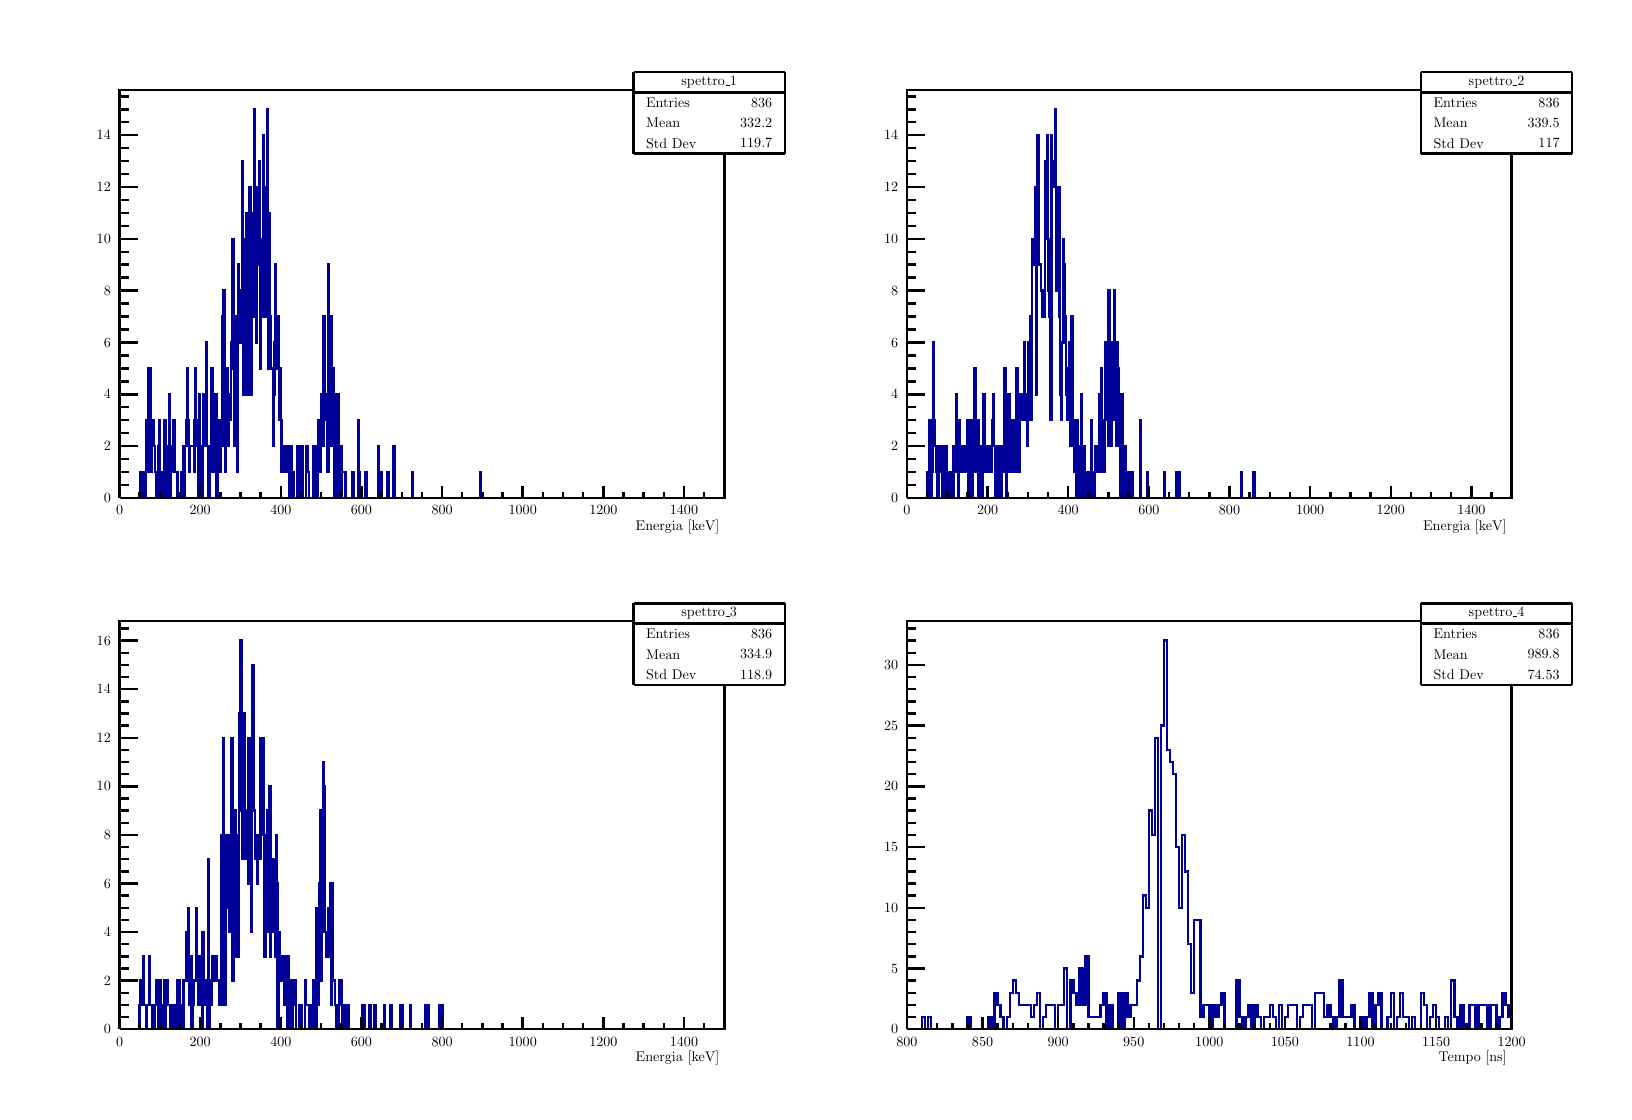
\begin{tikzpicture}
\pgfdeclareplotmark{cross} {
\pgfpathmoveto{\pgfpoint{-0.3\pgfplotmarksize}{\pgfplotmarksize}}
\pgfpathlineto{\pgfpoint{+0.3\pgfplotmarksize}{\pgfplotmarksize}}
\pgfpathlineto{\pgfpoint{+0.3\pgfplotmarksize}{0.3\pgfplotmarksize}}
\pgfpathlineto{\pgfpoint{+1\pgfplotmarksize}{0.3\pgfplotmarksize}}
\pgfpathlineto{\pgfpoint{+1\pgfplotmarksize}{-0.3\pgfplotmarksize}}
\pgfpathlineto{\pgfpoint{+0.3\pgfplotmarksize}{-0.3\pgfplotmarksize}}
\pgfpathlineto{\pgfpoint{+0.3\pgfplotmarksize}{-1.\pgfplotmarksize}}
\pgfpathlineto{\pgfpoint{-0.3\pgfplotmarksize}{-1.\pgfplotmarksize}}
\pgfpathlineto{\pgfpoint{-0.3\pgfplotmarksize}{-0.3\pgfplotmarksize}}
\pgfpathlineto{\pgfpoint{-1.\pgfplotmarksize}{-0.3\pgfplotmarksize}}
\pgfpathlineto{\pgfpoint{-1.\pgfplotmarksize}{0.3\pgfplotmarksize}}
\pgfpathlineto{\pgfpoint{-0.3\pgfplotmarksize}{0.3\pgfplotmarksize}}
\pgfpathclose
\pgfusepathqstroke
}
\pgfdeclareplotmark{cross*} {
\pgfpathmoveto{\pgfpoint{-0.3\pgfplotmarksize}{\pgfplotmarksize}}
\pgfpathlineto{\pgfpoint{+0.3\pgfplotmarksize}{\pgfplotmarksize}}
\pgfpathlineto{\pgfpoint{+0.3\pgfplotmarksize}{0.3\pgfplotmarksize}}
\pgfpathlineto{\pgfpoint{+1\pgfplotmarksize}{0.3\pgfplotmarksize}}
\pgfpathlineto{\pgfpoint{+1\pgfplotmarksize}{-0.3\pgfplotmarksize}}
\pgfpathlineto{\pgfpoint{+0.3\pgfplotmarksize}{-0.3\pgfplotmarksize}}
\pgfpathlineto{\pgfpoint{+0.3\pgfplotmarksize}{-1.\pgfplotmarksize}}
\pgfpathlineto{\pgfpoint{-0.3\pgfplotmarksize}{-1.\pgfplotmarksize}}
\pgfpathlineto{\pgfpoint{-0.3\pgfplotmarksize}{-0.3\pgfplotmarksize}}
\pgfpathlineto{\pgfpoint{-1.\pgfplotmarksize}{-0.3\pgfplotmarksize}}
\pgfpathlineto{\pgfpoint{-1.\pgfplotmarksize}{0.3\pgfplotmarksize}}
\pgfpathlineto{\pgfpoint{-0.3\pgfplotmarksize}{0.3\pgfplotmarksize}}
\pgfpathclose
\pgfusepathqfillstroke
}
\pgfdeclareplotmark{newstar} {
\pgfpathmoveto{\pgfqpoint{0pt}{\pgfplotmarksize}}
\pgfpathlineto{\pgfqpointpolar{44}{0.5\pgfplotmarksize}}
\pgfpathlineto{\pgfqpointpolar{18}{\pgfplotmarksize}}
\pgfpathlineto{\pgfqpointpolar{-20}{0.5\pgfplotmarksize}}
\pgfpathlineto{\pgfqpointpolar{-54}{\pgfplotmarksize}}
\pgfpathlineto{\pgfqpointpolar{-90}{0.5\pgfplotmarksize}}
\pgfpathlineto{\pgfqpointpolar{234}{\pgfplotmarksize}}
\pgfpathlineto{\pgfqpointpolar{198}{0.5\pgfplotmarksize}}
\pgfpathlineto{\pgfqpointpolar{162}{\pgfplotmarksize}}
\pgfpathlineto{\pgfqpointpolar{134}{0.5\pgfplotmarksize}}
\pgfpathclose
\pgfusepathqstroke
}
\pgfdeclareplotmark{newstar*} {
\pgfpathmoveto{\pgfqpoint{0pt}{\pgfplotmarksize}}
\pgfpathlineto{\pgfqpointpolar{44}{0.5\pgfplotmarksize}}
\pgfpathlineto{\pgfqpointpolar{18}{\pgfplotmarksize}}
\pgfpathlineto{\pgfqpointpolar{-20}{0.5\pgfplotmarksize}}
\pgfpathlineto{\pgfqpointpolar{-54}{\pgfplotmarksize}}
\pgfpathlineto{\pgfqpointpolar{-90}{0.5\pgfplotmarksize}}
\pgfpathlineto{\pgfqpointpolar{234}{\pgfplotmarksize}}
\pgfpathlineto{\pgfqpointpolar{198}{0.5\pgfplotmarksize}}
\pgfpathlineto{\pgfqpointpolar{162}{\pgfplotmarksize}}
\pgfpathlineto{\pgfqpointpolar{134}{0.5\pgfplotmarksize}}
\pgfpathclose
\pgfusepathqfillstroke
}
\definecolor{c}{rgb}{1,1,1};
\draw [color=c, fill=c] (0,0) rectangle (20,13.4957);
\draw [color=c, fill=c] (0.2,6.88281) rectangle (9.8,13.3607);
\draw [color=c, fill=c] (1.16,7.5306) rectangle (8.84,12.713);
\definecolor{c}{rgb}{0,0,0};
\draw [c,line width=0.9] (1.16,7.5306) -- (1.16,12.713) -- (8.84,12.713) -- (8.84,7.5306) -- (1.16,7.5306);
\definecolor{c}{rgb}{1,1,1};
\draw [color=c, fill=c] (1.16,7.5306) rectangle (8.84,12.713);
\definecolor{c}{rgb}{0,0,0};
\draw [c,line width=0.9] (1.16,7.5306) -- (1.16,12.713) -- (8.84,12.713) -- (8.84,7.5306) -- (1.16,7.5306);
\definecolor{c}{rgb}{0,0,0.6};
\draw [c,line width=0.9] (1.16,7.5306) -- (1.17024,7.5306) -- (1.17024,7.5306) -- (1.18048,7.5306) -- (1.18048,7.5306) -- (1.19072,7.5306) -- (1.19072,7.5306) -- (1.20096,7.5306) -- (1.20096,7.5306) -- (1.2112,7.5306) -- (1.2112,7.5306) --
 (1.22144,7.5306) -- (1.22144,7.5306) -- (1.23168,7.5306) -- (1.23168,7.5306) -- (1.24192,7.5306) -- (1.24192,7.5306) -- (1.25216,7.5306) -- (1.25216,7.5306) -- (1.2624,7.5306) -- (1.2624,7.5306) -- (1.27264,7.5306) -- (1.27264,7.5306) --
 (1.28288,7.5306) -- (1.28288,7.5306) -- (1.29312,7.5306) -- (1.29312,7.5306) -- (1.30336,7.5306) -- (1.30336,7.5306) -- (1.3136,7.5306) -- (1.3136,7.5306) -- (1.32384,7.5306) -- (1.32384,7.5306) -- (1.33408,7.5306) -- (1.33408,7.5306) --
 (1.34432,7.5306) -- (1.34432,7.5306) -- (1.35456,7.5306) -- (1.35456,7.5306) -- (1.3648,7.5306) -- (1.3648,7.5306) -- (1.37504,7.5306) -- (1.37504,7.5306) -- (1.38528,7.5306) -- (1.38528,7.5306) -- (1.39552,7.5306) -- (1.39552,7.5306) --
 (1.40576,7.5306) -- (1.40576,7.5306) -- (1.416,7.5306) -- (1.416,7.5306) -- (1.42624,7.5306) -- (1.42624,7.85964) -- (1.43648,7.85964) -- (1.43648,7.5306) -- (1.44672,7.5306) -- (1.44672,7.85964) -- (1.45696,7.85964) -- (1.45696,7.85964) --
 (1.4672,7.85964) -- (1.4672,7.5306) -- (1.47744,7.5306) -- (1.47744,7.5306) -- (1.48768,7.5306) -- (1.48768,7.85964) -- (1.49792,7.85964) -- (1.49792,8.51772) -- (1.50816,8.51772) -- (1.50816,8.51772) -- (1.5184,8.51772) -- (1.5184,7.85964) --
 (1.52864,7.85964) -- (1.52864,9.17579) -- (1.53888,9.17579) -- (1.53888,7.85964) -- (1.54912,7.85964) -- (1.54912,9.17579) -- (1.55936,9.17579) -- (1.55936,7.85964) -- (1.5696,7.85964) -- (1.5696,8.18868) -- (1.57984,8.18868) -- (1.57984,8.18868) --
 (1.59008,8.18868) -- (1.59008,8.51772) -- (1.60032,8.51772) -- (1.60032,8.18868) -- (1.61056,8.18868) -- (1.61056,7.85964) -- (1.6208,7.85964) -- (1.6208,7.5306) -- (1.63104,7.5306) -- (1.63104,7.85964) -- (1.64128,7.85964) -- (1.64128,7.5306) --
 (1.65152,7.5306) -- (1.65152,8.18868) -- (1.66176,8.18868) -- (1.66176,8.51772) -- (1.672,8.51772) -- (1.672,7.85964) -- (1.68224,7.85964) -- (1.68224,7.5306) -- (1.69248,7.5306) -- (1.69248,7.5306) -- (1.70272,7.5306) -- (1.70272,7.5306) --
 (1.71296,7.5306) -- (1.71296,7.85964) -- (1.7232,7.85964) -- (1.7232,7.85964) -- (1.73344,7.85964) -- (1.73344,8.51772) -- (1.74368,8.51772) -- (1.74368,7.5306) -- (1.75392,7.5306) -- (1.75392,7.85964) -- (1.76416,7.85964) -- (1.76416,7.5306) --
 (1.7744,7.5306) -- (1.7744,8.18868) -- (1.78464,8.18868) -- (1.78464,8.84675) -- (1.79488,8.84675) -- (1.79488,7.5306) -- (1.80512,7.5306) -- (1.80512,8.18868) -- (1.81536,8.18868) -- (1.81536,7.85964) -- (1.8256,7.85964) -- (1.8256,7.85964) --
 (1.83584,7.85964) -- (1.83584,8.18868) -- (1.84608,8.18868) -- (1.84608,8.51772) -- (1.85632,8.51772) -- (1.85632,7.85964) -- (1.86656,7.85964) -- (1.86656,7.85964) -- (1.8768,7.85964) -- (1.8768,7.85964) -- (1.88704,7.85964) -- (1.88704,7.85964) --
 (1.89728,7.85964) -- (1.89728,7.5306) -- (1.90752,7.5306) -- (1.90752,7.5306) -- (1.91776,7.5306) -- (1.91776,7.5306) -- (1.928,7.5306) -- (1.928,7.5306) -- (1.93824,7.5306) -- (1.93824,7.85964) -- (1.94848,7.85964) -- (1.94848,7.5306) --
 (1.95872,7.5306) -- (1.95872,7.85964) -- (1.96896,7.85964) -- (1.96896,8.18868) -- (1.9792,8.18868) -- (1.9792,7.5306) -- (1.98944,7.5306) -- (1.98944,8.18868) -- (1.99968,8.18868) -- (1.99968,8.18868) -- (2.00992,8.18868) -- (2.00992,8.51772) --
 (2.02016,8.51772) -- (2.02016,9.17579) -- (2.0304,9.17579) -- (2.0304,8.51772) -- (2.04064,8.51772) -- (2.04064,7.85964) -- (2.05088,7.85964) -- (2.05088,8.18868) -- (2.06112,8.18868) -- (2.06112,8.18868) -- (2.07136,8.18868) -- (2.07136,8.18868) --
 (2.0816,8.18868) -- (2.0816,8.18868) -- (2.09184,8.18868) -- (2.09184,8.18868) -- (2.10208,8.18868) -- (2.10208,7.85964) -- (2.11232,7.85964) -- (2.11232,8.51772) -- (2.12256,8.51772) -- (2.12256,9.17579) -- (2.1328,9.17579) -- (2.1328,8.18868) --
 (2.14304,8.18868) -- (2.14304,8.51772) -- (2.15328,8.51772) -- (2.15328,7.85964) -- (2.16352,7.85964) -- (2.16352,7.5306) -- (2.17376,7.5306) -- (2.17376,8.84675) -- (2.184,8.84675) -- (2.184,7.5306) -- (2.19424,7.5306) -- (2.19424,8.18868) --
 (2.20448,8.18868) -- (2.20448,7.5306) -- (2.21472,7.5306) -- (2.21472,8.18868) -- (2.22496,8.18868) -- (2.22496,8.84675) -- (2.2352,8.84675) -- (2.2352,8.18868) -- (2.24544,8.18868) -- (2.24544,8.51772) -- (2.25568,8.51772) -- (2.25568,9.50483) --
 (2.26592,9.50483) -- (2.26592,8.18868) -- (2.27616,8.18868) -- (2.27616,8.18868) -- (2.2864,8.18868) -- (2.2864,7.5306) -- (2.29664,7.5306) -- (2.29664,7.5306) -- (2.30688,7.5306) -- (2.30688,7.85964) -- (2.31712,7.85964) -- (2.31712,8.18868) --
 (2.32736,8.18868) -- (2.32736,9.17579) -- (2.3376,9.17579) -- (2.3376,8.84675) -- (2.34784,8.84675) -- (2.34784,7.85964) -- (2.35808,7.85964) -- (2.35808,8.18868) -- (2.36832,8.18868) -- (2.36832,7.85964) -- (2.37856,7.85964) -- (2.37856,8.84675) --
 (2.3888,8.84675) -- (2.3888,7.5306) -- (2.39904,7.5306) -- (2.39904,7.5306) -- (2.40928,7.5306) -- (2.40928,8.18868) -- (2.41952,8.18868) -- (2.41952,7.85964) -- (2.42976,7.85964) -- (2.42976,8.51772) -- (2.44,8.51772) -- (2.44,7.85964) --
 (2.45024,7.85964) -- (2.45024,8.51772) -- (2.46048,8.51772) -- (2.46048,9.83387) -- (2.47072,9.83387) -- (2.47072,8.18868) -- (2.48096,8.18868) -- (2.48096,10.1629) -- (2.4912,10.1629) -- (2.4912,9.50483) -- (2.50144,9.50483) -- (2.50144,7.85964) --
 (2.51168,7.85964) -- (2.51168,8.18868) -- (2.52192,8.18868) -- (2.52192,9.17579) -- (2.53216,9.17579) -- (2.53216,8.18868) -- (2.5424,8.18868) -- (2.5424,8.84675) -- (2.55264,8.84675) -- (2.55264,8.84675) -- (2.56288,8.84675) -- (2.56288,8.51772) --
 (2.57312,8.51772) -- (2.57312,9.50483) -- (2.58336,9.50483) -- (2.58336,9.17579) -- (2.5936,9.17579) -- (2.5936,10.821) -- (2.60384,10.821) -- (2.60384,9.50483) -- (2.61408,9.50483) -- (2.61408,8.18868) -- (2.62432,8.18868) -- (2.62432,9.17579) --
 (2.63456,9.17579) -- (2.63456,9.83387) -- (2.6448,9.83387) -- (2.6448,9.17579) -- (2.65504,9.17579) -- (2.65504,7.85964) -- (2.66528,7.85964) -- (2.66528,10.4919) -- (2.67552,10.4919) -- (2.67552,10.1629) -- (2.68576,10.1629) -- (2.68576,9.50483) --
 (2.696,9.50483) -- (2.696,9.50483) -- (2.70624,9.50483) -- (2.70624,9.83387) -- (2.71648,9.83387) -- (2.71648,11.8081) -- (2.72672,11.8081) -- (2.72672,10.821) -- (2.73696,10.821) -- (2.73696,8.84675) -- (2.7472,8.84675) -- (2.7472,8.84675) --
 (2.75744,8.84675) -- (2.75744,8.84675) -- (2.76768,8.84675) -- (2.76768,11.15) -- (2.77792,11.15) -- (2.77792,9.50483) -- (2.78816,9.50483) -- (2.78816,8.84675) -- (2.7984,8.84675) -- (2.7984,9.83387) -- (2.80864,9.83387) -- (2.80864,11.4791) --
 (2.81888,11.4791) -- (2.81888,11.4791) -- (2.82912,11.4791) -- (2.82912,8.84675) -- (2.83936,8.84675) -- (2.83936,10.4919) -- (2.8496,10.4919) -- (2.8496,11.15) -- (2.85984,11.15) -- (2.85984,9.83387) -- (2.87008,9.83387) -- (2.87008,12.4662) --
 (2.88032,12.4662) -- (2.88032,10.821) -- (2.89056,10.821) -- (2.89056,9.50483) -- (2.9008,9.50483) -- (2.9008,10.4919) -- (2.91104,10.4919) -- (2.91104,11.4791) -- (2.92128,11.4791) -- (2.92128,10.821) -- (2.93152,10.821) -- (2.93152,11.8081) --
 (2.94176,11.8081) -- (2.94176,9.17579) -- (2.952,9.17579) -- (2.952,9.83387) -- (2.96224,9.83387) -- (2.96224,10.821) -- (2.97248,10.821) -- (2.97248,10.1629) -- (2.98272,10.1629) -- (2.98272,12.1371) -- (2.99296,12.1371) -- (2.99296,10.821) --
 (3.0032,10.821) -- (3.0032,9.83387) -- (3.01344,9.83387) -- (3.01344,11.4791) -- (3.02368,11.4791) -- (3.02368,10.821) -- (3.03392,10.821) -- (3.03392,12.4662) -- (3.04416,12.4662) -- (3.04416,9.17579) -- (3.0544,9.17579) -- (3.0544,11.15) --
 (3.06464,11.15) -- (3.06464,9.83387) -- (3.07488,9.83387) -- (3.07488,9.83387) -- (3.08512,9.83387) -- (3.08512,9.17579) -- (3.09536,9.17579) -- (3.09536,9.17579) -- (3.1056,9.17579) -- (3.1056,8.18868) -- (3.11584,8.18868) -- (3.11584,8.84675) --
 (3.12608,8.84675) -- (3.12608,9.50483) -- (3.13632,9.50483) -- (3.13632,10.4919) -- (3.14656,10.4919) -- (3.14656,9.50483) -- (3.1568,9.50483) -- (3.1568,9.83387) -- (3.16704,9.83387) -- (3.16704,9.17579) -- (3.17728,9.17579) -- (3.17728,9.83387) --
 (3.18752,9.83387) -- (3.18752,8.51772) -- (3.19776,8.51772) -- (3.19776,9.17579) -- (3.208,9.17579) -- (3.208,8.51772) -- (3.21824,8.51772) -- (3.21824,7.85964) -- (3.22848,7.85964) -- (3.22848,8.18868) -- (3.23872,8.18868) -- (3.23872,7.85964) --
 (3.24896,7.85964) -- (3.24896,7.85964) -- (3.2592,7.85964) -- (3.2592,8.18868) -- (3.26944,8.18868) -- (3.26944,7.85964) -- (3.27968,7.85964) -- (3.27968,8.18868) -- (3.28992,8.18868) -- (3.28992,7.85964) -- (3.30016,7.85964) -- (3.30016,8.18868) --
 (3.3104,8.18868) -- (3.3104,7.5306) -- (3.32064,7.5306) -- (3.32064,8.18868) -- (3.33088,8.18868) -- (3.33088,7.85964) -- (3.34112,7.85964) -- (3.34112,8.18868) -- (3.35136,8.18868) -- (3.35136,7.5306) -- (3.3616,7.5306) -- (3.3616,7.85964) --
 (3.37184,7.85964) -- (3.37184,7.5306) -- (3.38208,7.5306) -- (3.38208,7.5306) -- (3.39232,7.5306) -- (3.39232,7.5306) -- (3.40256,7.5306) -- (3.40256,7.5306) -- (3.4128,7.5306) -- (3.4128,8.18868) -- (3.42304,8.18868) -- (3.42304,7.85964) --
 (3.43328,7.85964) -- (3.43328,7.5306) -- (3.44352,7.5306) -- (3.44352,8.18868) -- (3.45376,8.18868) -- (3.45376,7.85964) -- (3.464,7.85964) -- (3.464,7.5306) -- (3.47424,7.5306) -- (3.47424,8.18868) -- (3.48448,8.18868) -- (3.48448,7.5306) --
 (3.49472,7.5306) -- (3.49472,7.5306) -- (3.50496,7.5306) -- (3.50496,7.5306) -- (3.5152,7.5306) -- (3.5152,7.5306) -- (3.52544,7.5306) -- (3.52544,7.85964) -- (3.53568,7.85964) -- (3.53568,8.18868) -- (3.54592,8.18868) -- (3.54592,8.18868) --
 (3.55616,8.18868) -- (3.55616,7.85964) -- (3.5664,7.85964) -- (3.5664,7.5306) -- (3.57664,7.5306) -- (3.57664,7.5306) -- (3.58688,7.5306) -- (3.58688,7.5306) -- (3.59712,7.5306) -- (3.59712,7.5306) -- (3.60736,7.5306) -- (3.60736,7.5306) --
 (3.6176,7.5306) -- (3.6176,8.18868) -- (3.62784,8.18868) -- (3.62784,7.85964) -- (3.63808,7.85964) -- (3.63808,7.5306) -- (3.64832,7.5306) -- (3.64832,8.18868) -- (3.65856,8.18868) -- (3.65856,8.18868) -- (3.6688,8.18868) -- (3.6688,7.5306) --
 (3.67904,7.5306) -- (3.67904,8.51772) -- (3.68928,8.51772) -- (3.68928,8.18868) -- (3.69952,8.18868) -- (3.69952,7.85964) -- (3.70976,7.85964) -- (3.70976,8.51772) -- (3.72,8.51772) -- (3.72,8.84675) -- (3.73024,8.84675) -- (3.73024,8.51772) --
 (3.74048,8.51772) -- (3.74048,8.18868) -- (3.75072,8.18868) -- (3.75072,9.83387) -- (3.76096,9.83387) -- (3.76096,8.51772) -- (3.7712,8.51772) -- (3.7712,8.84675) -- (3.78144,8.84675) -- (3.78144,8.84675) -- (3.79168,8.84675) -- (3.79168,8.51772) --
 (3.80192,8.51772) -- (3.80192,7.85964) -- (3.81216,7.85964) -- (3.81216,10.4919) -- (3.8224,10.4919) -- (3.8224,9.83387) -- (3.83264,9.83387) -- (3.83264,8.51772) -- (3.84288,8.51772) -- (3.84288,9.83387) -- (3.85312,9.83387) -- (3.85312,8.18868) --
 (3.86336,8.18868) -- (3.86336,8.84675) -- (3.8736,8.84675) -- (3.8736,9.17579) -- (3.88384,9.17579) -- (3.88384,7.5306) -- (3.89408,7.5306) -- (3.89408,8.51772) -- (3.90432,8.51772) -- (3.90432,8.84675) -- (3.91456,8.84675) -- (3.91456,8.18868) --
 (3.9248,8.18868) -- (3.9248,7.5306) -- (3.93504,7.5306) -- (3.93504,8.84675) -- (3.94528,8.84675) -- (3.94528,7.5306) -- (3.95552,7.5306) -- (3.95552,7.5306) -- (3.96576,7.5306) -- (3.96576,7.5306) -- (3.976,7.5306) -- (3.976,8.18868) --
 (3.98624,8.18868) -- (3.98624,7.85964) -- (3.99648,7.85964) -- (3.99648,7.85964) -- (4.00672,7.85964) -- (4.00672,7.85964) -- (4.01696,7.85964) -- (4.01696,7.85964) -- (4.0272,7.85964) -- (4.0272,7.5306) -- (4.03744,7.5306) -- (4.03744,7.5306) --
 (4.04768,7.5306) -- (4.04768,7.5306) -- (4.05792,7.5306) -- (4.05792,7.5306) -- (4.06816,7.5306) -- (4.06816,7.5306) -- (4.0784,7.5306) -- (4.0784,7.5306) -- (4.08864,7.5306) -- (4.08864,7.5306) -- (4.09888,7.5306) -- (4.09888,7.5306) --
 (4.10912,7.5306) -- (4.10912,7.85964) -- (4.11936,7.85964) -- (4.11936,7.5306) -- (4.1296,7.5306) -- (4.1296,7.85964) -- (4.13984,7.85964) -- (4.13984,7.5306) -- (4.15008,7.5306) -- (4.15008,7.5306) -- (4.16032,7.5306) -- (4.16032,7.5306) --
 (4.17056,7.5306) -- (4.17056,7.5306) -- (4.1808,7.5306) -- (4.1808,7.5306) -- (4.19104,7.5306) -- (4.19104,8.51772) -- (4.20128,8.51772) -- (4.20128,7.85964) -- (4.21152,7.85964) -- (4.21152,7.5306) -- (4.22176,7.5306) -- (4.22176,7.5306) --
 (4.232,7.5306) -- (4.232,7.5306) -- (4.24224,7.5306) -- (4.24224,7.5306) -- (4.25248,7.5306) -- (4.25248,7.5306) -- (4.26272,7.5306) -- (4.26272,7.5306) -- (4.27296,7.5306) -- (4.27296,7.5306) -- (4.2832,7.5306) -- (4.2832,7.85964) --
 (4.29344,7.85964) -- (4.29344,7.85964) -- (4.30368,7.85964) -- (4.30368,7.5306) -- (4.31392,7.5306) -- (4.31392,7.5306) -- (4.32416,7.5306) -- (4.32416,7.5306) -- (4.3344,7.5306) -- (4.3344,7.5306) -- (4.34464,7.5306) -- (4.34464,7.5306) --
 (4.35488,7.5306) -- (4.35488,7.5306) -- (4.36512,7.5306) -- (4.36512,7.5306) -- (4.37536,7.5306) -- (4.37536,7.5306) -- (4.3856,7.5306) -- (4.3856,7.5306) -- (4.39584,7.5306) -- (4.39584,7.5306) -- (4.40608,7.5306) -- (4.40608,7.5306) --
 (4.41632,7.5306) -- (4.41632,7.5306) -- (4.42656,7.5306) -- (4.42656,7.5306) -- (4.4368,7.5306) -- (4.4368,7.5306) -- (4.44704,7.5306) -- (4.44704,8.18868) -- (4.45728,8.18868) -- (4.45728,7.5306) -- (4.46752,7.5306) -- (4.46752,7.5306) --
 (4.47776,7.5306) -- (4.47776,7.85964) -- (4.488,7.85964) -- (4.488,7.5306) -- (4.49824,7.5306) -- (4.49824,7.5306) -- (4.50848,7.5306) -- (4.50848,7.5306) -- (4.51872,7.5306) -- (4.51872,7.5306) -- (4.52896,7.5306) -- (4.52896,7.5306) --
 (4.5392,7.5306) -- (4.5392,7.5306) -- (4.54944,7.5306) -- (4.54944,7.5306) -- (4.55968,7.5306) -- (4.55968,7.85964) -- (4.56992,7.85964) -- (4.56992,7.85964) -- (4.58016,7.85964) -- (4.58016,7.5306) -- (4.5904,7.5306) -- (4.5904,7.5306) --
 (4.60064,7.5306) -- (4.60064,7.5306) -- (4.61088,7.5306) -- (4.61088,7.5306) -- (4.62112,7.5306) -- (4.62112,7.5306) -- (4.63136,7.5306) -- (4.63136,7.85964) -- (4.6416,7.85964) -- (4.6416,8.18868) -- (4.65184,8.18868) -- (4.65184,7.5306) --
 (4.66208,7.5306) -- (4.66208,7.5306) -- (4.67232,7.5306) -- (4.67232,7.5306) -- (4.68256,7.5306) -- (4.68256,7.5306) -- (4.6928,7.5306) -- (4.6928,7.5306) -- (4.70304,7.5306) -- (4.70304,7.5306) -- (4.71328,7.5306) -- (4.71328,7.5306) --
 (4.72352,7.5306) -- (4.72352,7.5306) -- (4.73376,7.5306) -- (4.73376,7.5306) -- (4.744,7.5306) -- (4.744,7.5306) -- (4.75424,7.5306) -- (4.75424,7.5306) -- (4.76448,7.5306) -- (4.76448,7.5306) -- (4.77472,7.5306) -- (4.77472,7.5306) --
 (4.78496,7.5306) -- (4.78496,7.5306) -- (4.7952,7.5306) -- (4.7952,7.5306) -- (4.80544,7.5306) -- (4.80544,7.5306) -- (4.81568,7.5306) -- (4.81568,7.5306) -- (4.82592,7.5306) -- (4.82592,7.5306) -- (4.83616,7.5306) -- (4.83616,7.5306) --
 (4.8464,7.5306) -- (4.8464,7.5306) -- (4.85664,7.5306) -- (4.85664,7.5306) -- (4.86688,7.5306) -- (4.86688,7.5306) -- (4.87712,7.5306) -- (4.87712,7.85964) -- (4.88736,7.85964) -- (4.88736,7.5306) -- (4.8976,7.5306) -- (4.8976,7.5306) --
 (4.90784,7.5306) -- (4.90784,7.5306) -- (4.91808,7.5306) -- (4.91808,7.5306) -- (4.92832,7.5306) -- (4.92832,7.5306) -- (4.93856,7.5306) -- (4.93856,7.5306) -- (4.9488,7.5306) -- (4.9488,7.5306) -- (4.95904,7.5306) -- (4.95904,7.5306) --
 (4.96928,7.5306) -- (4.96928,7.5306) -- (4.97952,7.5306) -- (4.97952,7.5306) -- (4.98976,7.5306) -- (4.98976,7.5306) -- (5,7.5306) -- (5,7.5306) -- (5.01024,7.5306) -- (5.01024,7.5306) -- (5.02048,7.5306) -- (5.02048,7.5306) -- (5.03072,7.5306) --
 (5.03072,7.5306) -- (5.04096,7.5306) -- (5.04096,7.5306) -- (5.0512,7.5306) -- (5.0512,7.5306) -- (5.06144,7.5306) -- (5.06144,7.5306) -- (5.07168,7.5306) -- (5.07168,7.5306) -- (5.08192,7.5306) -- (5.08192,7.5306) -- (5.09216,7.5306) --
 (5.09216,7.5306) -- (5.1024,7.5306) -- (5.1024,7.5306) -- (5.11264,7.5306) -- (5.11264,7.5306) -- (5.12288,7.5306) -- (5.12288,7.5306) -- (5.13312,7.5306) -- (5.13312,7.5306) -- (5.14336,7.5306) -- (5.14336,7.5306) -- (5.1536,7.5306) --
 (5.1536,7.5306) -- (5.16384,7.5306) -- (5.16384,7.5306) -- (5.17408,7.5306) -- (5.17408,7.5306) -- (5.18432,7.5306) -- (5.18432,7.5306) -- (5.19456,7.5306) -- (5.19456,7.5306) -- (5.2048,7.5306) -- (5.2048,7.5306) -- (5.21504,7.5306) --
 (5.21504,7.5306) -- (5.22528,7.5306) -- (5.22528,7.5306) -- (5.23552,7.5306) -- (5.23552,7.5306) -- (5.24576,7.5306) -- (5.24576,7.5306) -- (5.256,7.5306) -- (5.256,7.5306) -- (5.26624,7.5306) -- (5.26624,7.5306) -- (5.27648,7.5306) --
 (5.27648,7.5306) -- (5.28672,7.5306) -- (5.28672,7.5306) -- (5.29696,7.5306) -- (5.29696,7.5306) -- (5.3072,7.5306) -- (5.3072,7.5306) -- (5.31744,7.5306) -- (5.31744,7.5306) -- (5.32768,7.5306) -- (5.32768,7.5306) -- (5.33792,7.5306) --
 (5.33792,7.5306) -- (5.34816,7.5306) -- (5.34816,7.5306) -- (5.3584,7.5306) -- (5.3584,7.5306) -- (5.36864,7.5306) -- (5.36864,7.5306) -- (5.37888,7.5306) -- (5.37888,7.5306) -- (5.38912,7.5306) -- (5.38912,7.5306) -- (5.39936,7.5306) --
 (5.39936,7.5306) -- (5.4096,7.5306) -- (5.4096,7.5306) -- (5.41984,7.5306) -- (5.41984,7.5306) -- (5.43008,7.5306) -- (5.43008,7.5306) -- (5.44032,7.5306) -- (5.44032,7.5306) -- (5.45056,7.5306) -- (5.45056,7.5306) -- (5.4608,7.5306) --
 (5.4608,7.5306) -- (5.47104,7.5306) -- (5.47104,7.5306) -- (5.48128,7.5306) -- (5.48128,7.5306) -- (5.49152,7.5306) -- (5.49152,7.5306) -- (5.50176,7.5306) -- (5.50176,7.5306) -- (5.512,7.5306) -- (5.512,7.5306) -- (5.52224,7.5306) --
 (5.52224,7.5306) -- (5.53248,7.5306) -- (5.53248,7.5306) -- (5.54272,7.5306) -- (5.54272,7.5306) -- (5.55296,7.5306) -- (5.55296,7.5306) -- (5.5632,7.5306) -- (5.5632,7.5306) -- (5.57344,7.5306) -- (5.57344,7.5306) -- (5.58368,7.5306) --
 (5.58368,7.5306) -- (5.59392,7.5306) -- (5.59392,7.5306) -- (5.60416,7.5306) -- (5.60416,7.5306) -- (5.6144,7.5306) -- (5.6144,7.5306) -- (5.62464,7.5306) -- (5.62464,7.5306) -- (5.63488,7.5306) -- (5.63488,7.5306) -- (5.64512,7.5306) --
 (5.64512,7.5306) -- (5.65536,7.5306) -- (5.65536,7.5306) -- (5.6656,7.5306) -- (5.6656,7.5306) -- (5.67584,7.5306) -- (5.67584,7.5306) -- (5.68608,7.5306) -- (5.68608,7.5306) -- (5.69632,7.5306) -- (5.69632,7.5306) -- (5.70656,7.5306) --
 (5.70656,7.5306) -- (5.7168,7.5306) -- (5.7168,7.5306) -- (5.72704,7.5306) -- (5.72704,7.5306) -- (5.73728,7.5306) -- (5.73728,7.85964) -- (5.74752,7.85964) -- (5.74752,7.5306) -- (5.75776,7.5306) -- (5.75776,7.5306) -- (5.768,7.5306) --
 (5.768,7.5306) -- (5.77824,7.5306) -- (5.77824,7.5306) -- (5.78848,7.5306) -- (5.78848,7.5306) -- (5.79872,7.5306) -- (5.79872,7.5306) -- (5.80896,7.5306) -- (5.80896,7.5306) -- (5.8192,7.5306) -- (5.8192,7.5306) -- (5.82944,7.5306) --
 (5.82944,7.5306) -- (5.83968,7.5306) -- (5.83968,7.5306) -- (5.84992,7.5306) -- (5.84992,7.5306) -- (5.86016,7.5306) -- (5.86016,7.5306) -- (5.8704,7.5306) -- (5.8704,7.5306) -- (5.88064,7.5306) -- (5.88064,7.5306) -- (5.89088,7.5306) --
 (5.89088,7.5306) -- (5.90112,7.5306) -- (5.90112,7.5306) -- (5.91136,7.5306) -- (5.91136,7.5306) -- (5.9216,7.5306) -- (5.9216,7.5306) -- (5.93184,7.5306) -- (5.93184,7.5306) -- (5.94208,7.5306) -- (5.94208,7.5306) -- (5.95232,7.5306) --
 (5.95232,7.5306) -- (5.96256,7.5306) -- (5.96256,7.5306) -- (5.9728,7.5306) -- (5.9728,7.5306) -- (5.98304,7.5306) -- (5.98304,7.5306) -- (5.99328,7.5306) -- (5.99328,7.5306) -- (6.00352,7.5306) -- (6.00352,7.5306) -- (6.01376,7.5306) --
 (6.01376,7.5306) -- (6.024,7.5306) -- (6.024,7.5306) -- (6.03424,7.5306) -- (6.03424,7.5306) -- (6.04448,7.5306) -- (6.04448,7.5306) -- (6.05472,7.5306) -- (6.05472,7.5306) -- (6.06496,7.5306) -- (6.06496,7.5306) -- (6.0752,7.5306) --
 (6.0752,7.5306) -- (6.08544,7.5306) -- (6.08544,7.5306) -- (6.09568,7.5306) -- (6.09568,7.5306) -- (6.10592,7.5306) -- (6.10592,7.5306) -- (6.11616,7.5306) -- (6.11616,7.5306) -- (6.1264,7.5306) -- (6.1264,7.5306) -- (6.13664,7.5306) --
 (6.13664,7.5306) -- (6.14688,7.5306) -- (6.14688,7.5306) -- (6.15712,7.5306) -- (6.15712,7.5306) -- (6.16736,7.5306) -- (6.16736,7.5306) -- (6.1776,7.5306) -- (6.1776,7.5306) -- (6.18784,7.5306) -- (6.18784,7.5306) -- (6.19808,7.5306) --
 (6.19808,7.5306) -- (6.20832,7.5306) -- (6.20832,7.5306) -- (6.21856,7.5306) -- (6.21856,7.5306) -- (6.2288,7.5306) -- (6.2288,7.5306) -- (6.23904,7.5306) -- (6.23904,7.5306) -- (6.24928,7.5306) -- (6.24928,7.5306) -- (6.25952,7.5306) --
 (6.25952,7.5306) -- (6.26976,7.5306) -- (6.26976,7.5306) -- (6.28,7.5306) -- (6.28,7.5306) -- (6.29024,7.5306) -- (6.29024,7.5306) -- (6.30048,7.5306) -- (6.30048,7.5306) -- (6.31072,7.5306) -- (6.31072,7.5306) -- (6.32096,7.5306) --
 (6.32096,7.5306) -- (6.3312,7.5306) -- (6.3312,7.5306) -- (6.34144,7.5306) -- (6.34144,7.5306) -- (6.35168,7.5306) -- (6.35168,7.5306) -- (6.36192,7.5306) -- (6.36192,7.5306) -- (6.37216,7.5306) -- (6.37216,7.5306) -- (6.3824,7.5306) --
 (6.3824,7.5306) -- (6.39264,7.5306) -- (6.39264,7.5306) -- (6.40288,7.5306) -- (6.40288,7.5306) -- (6.41312,7.5306) -- (6.41312,7.5306) -- (6.42336,7.5306) -- (6.42336,7.5306) -- (6.4336,7.5306) -- (6.4336,7.5306) -- (6.44384,7.5306) --
 (6.44384,7.5306) -- (6.45408,7.5306) -- (6.45408,7.5306) -- (6.46432,7.5306) -- (6.46432,7.5306) -- (6.47456,7.5306) -- (6.47456,7.5306) -- (6.4848,7.5306) -- (6.4848,7.5306) -- (6.49504,7.5306) -- (6.49504,7.5306) -- (6.50528,7.5306) --
 (6.50528,7.5306) -- (6.51552,7.5306) -- (6.51552,7.5306) -- (6.52576,7.5306) -- (6.52576,7.5306) -- (6.536,7.5306) -- (6.536,7.5306) -- (6.54624,7.5306) -- (6.54624,7.5306) -- (6.55648,7.5306) -- (6.55648,7.5306) -- (6.56672,7.5306) --
 (6.56672,7.5306) -- (6.57696,7.5306) -- (6.57696,7.5306) -- (6.5872,7.5306) -- (6.5872,7.5306) -- (6.59744,7.5306) -- (6.59744,7.5306) -- (6.60768,7.5306) -- (6.60768,7.5306) -- (6.61792,7.5306) -- (6.61792,7.5306) -- (6.62816,7.5306) --
 (6.62816,7.5306) -- (6.6384,7.5306) -- (6.6384,7.5306) -- (6.64864,7.5306) -- (6.64864,7.5306) -- (6.65888,7.5306) -- (6.65888,7.5306) -- (6.66912,7.5306) -- (6.66912,7.5306) -- (6.67936,7.5306) -- (6.67936,7.5306) -- (6.6896,7.5306) --
 (6.6896,7.5306) -- (6.69984,7.5306) -- (6.69984,7.5306) -- (6.71008,7.5306) -- (6.71008,7.5306) -- (6.72032,7.5306) -- (6.72032,7.5306) -- (6.73056,7.5306) -- (6.73056,7.5306) -- (6.7408,7.5306) -- (6.7408,7.5306) -- (6.75104,7.5306) --
 (6.75104,7.5306) -- (6.76128,7.5306) -- (6.76128,7.5306) -- (6.77152,7.5306) -- (6.77152,7.5306) -- (6.78176,7.5306) -- (6.78176,7.5306) -- (6.792,7.5306) -- (6.792,7.5306) -- (6.80224,7.5306) -- (6.80224,7.5306) -- (6.81248,7.5306) --
 (6.81248,7.5306) -- (6.82272,7.5306) -- (6.82272,7.5306) -- (6.83296,7.5306) -- (6.83296,7.5306) -- (6.8432,7.5306) -- (6.8432,7.5306) -- (6.85344,7.5306) -- (6.85344,7.5306) -- (6.86368,7.5306) -- (6.86368,7.5306) -- (6.87392,7.5306) --
 (6.87392,7.5306) -- (6.88416,7.5306) -- (6.88416,7.5306) -- (6.8944,7.5306) -- (6.8944,7.5306) -- (6.90464,7.5306) -- (6.90464,7.5306) -- (6.91488,7.5306) -- (6.91488,7.5306) -- (6.92512,7.5306) -- (6.92512,7.5306) -- (6.93536,7.5306) --
 (6.93536,7.5306) -- (6.9456,7.5306) -- (6.9456,7.5306) -- (6.95584,7.5306) -- (6.95584,7.5306) -- (6.96608,7.5306) -- (6.96608,7.5306) -- (6.97632,7.5306) -- (6.97632,7.5306) -- (6.98656,7.5306) -- (6.98656,7.5306) -- (6.9968,7.5306) --
 (6.9968,7.5306) -- (7.00704,7.5306) -- (7.00704,7.5306) -- (7.01728,7.5306) -- (7.01728,7.5306) -- (7.02752,7.5306) -- (7.02752,7.5306) -- (7.03776,7.5306) -- (7.03776,7.5306) -- (7.048,7.5306) -- (7.048,7.5306) -- (7.05824,7.5306) --
 (7.05824,7.5306) -- (7.06848,7.5306) -- (7.06848,7.5306) -- (7.07872,7.5306) -- (7.07872,7.5306) -- (7.08896,7.5306) -- (7.08896,7.5306) -- (7.0992,7.5306) -- (7.0992,7.5306) -- (7.10944,7.5306) -- (7.10944,7.5306) -- (7.11968,7.5306) --
 (7.11968,7.5306) -- (7.12992,7.5306) -- (7.12992,7.5306) -- (7.14016,7.5306) -- (7.14016,7.5306) -- (7.1504,7.5306) -- (7.1504,7.5306) -- (7.16064,7.5306) -- (7.16064,7.5306) -- (7.17088,7.5306) -- (7.17088,7.5306) -- (7.18112,7.5306) --
 (7.18112,7.5306) -- (7.19136,7.5306) -- (7.19136,7.5306) -- (7.2016,7.5306) -- (7.2016,7.5306) -- (7.21184,7.5306) -- (7.21184,7.5306) -- (7.22208,7.5306) -- (7.22208,7.5306) -- (7.23232,7.5306) -- (7.23232,7.5306) -- (7.24256,7.5306) --
 (7.24256,7.5306) -- (7.2528,7.5306) -- (7.2528,7.5306) -- (7.26304,7.5306) -- (7.26304,7.5306) -- (7.27328,7.5306) -- (7.27328,7.5306) -- (7.28352,7.5306) -- (7.28352,7.5306) -- (7.29376,7.5306) -- (7.29376,7.5306) -- (7.304,7.5306) --
 (7.304,7.5306) -- (7.31424,7.5306) -- (7.31424,7.5306) -- (7.32448,7.5306) -- (7.32448,7.5306) -- (7.33472,7.5306) -- (7.33472,7.5306) -- (7.34496,7.5306) -- (7.34496,7.5306) -- (7.3552,7.5306) -- (7.3552,7.5306) -- (7.36544,7.5306) --
 (7.36544,7.5306) -- (7.37568,7.5306) -- (7.37568,7.5306) -- (7.38592,7.5306) -- (7.38592,7.5306) -- (7.39616,7.5306) -- (7.39616,7.5306) -- (7.4064,7.5306) -- (7.4064,7.5306) -- (7.41664,7.5306) -- (7.41664,7.5306) -- (7.42688,7.5306) --
 (7.42688,7.5306) -- (7.43712,7.5306) -- (7.43712,7.5306) -- (7.44736,7.5306) -- (7.44736,7.5306) -- (7.4576,7.5306) -- (7.4576,7.5306) -- (7.46784,7.5306) -- (7.46784,7.5306) -- (7.47808,7.5306) -- (7.47808,7.5306) -- (7.48832,7.5306) --
 (7.48832,7.5306) -- (7.49856,7.5306) -- (7.49856,7.5306) -- (7.5088,7.5306) -- (7.5088,7.5306) -- (7.51904,7.5306) -- (7.51904,7.5306) -- (7.52928,7.5306) -- (7.52928,7.5306) -- (7.53952,7.5306) -- (7.53952,7.5306) -- (7.54976,7.5306) --
 (7.54976,7.5306) -- (7.56,7.5306) -- (7.56,7.5306) -- (7.57024,7.5306) -- (7.57024,7.5306) -- (7.58048,7.5306) -- (7.58048,7.5306) -- (7.59072,7.5306) -- (7.59072,7.5306) -- (7.60096,7.5306) -- (7.60096,7.5306) -- (7.6112,7.5306) -- (7.6112,7.5306)
 -- (7.62144,7.5306) -- (7.62144,7.5306) -- (7.63168,7.5306) -- (7.63168,7.5306) -- (7.64192,7.5306) -- (7.64192,7.5306) -- (7.65216,7.5306) -- (7.65216,7.5306) -- (7.6624,7.5306) -- (7.6624,7.5306) -- (7.67264,7.5306) -- (7.67264,7.5306) --
 (7.68288,7.5306) -- (7.68288,7.5306) -- (7.69312,7.5306) -- (7.69312,7.5306) -- (7.70336,7.5306) -- (7.70336,7.5306) -- (7.7136,7.5306) -- (7.7136,7.5306) -- (7.72384,7.5306) -- (7.72384,7.5306) -- (7.73408,7.5306) -- (7.73408,7.5306) --
 (7.74432,7.5306) -- (7.74432,7.5306) -- (7.75456,7.5306) -- (7.75456,7.5306) -- (7.7648,7.5306) -- (7.7648,7.5306) -- (7.77504,7.5306) -- (7.77504,7.5306) -- (7.78528,7.5306) -- (7.78528,7.5306) -- (7.79552,7.5306) -- (7.79552,7.5306) --
 (7.80576,7.5306) -- (7.80576,7.5306) -- (7.816,7.5306) -- (7.816,7.5306) -- (7.82624,7.5306) -- (7.82624,7.5306) -- (7.83648,7.5306) -- (7.83648,7.5306) -- (7.84672,7.5306) -- (7.84672,7.5306) -- (7.85696,7.5306) -- (7.85696,7.5306) --
 (7.8672,7.5306) -- (7.8672,7.5306) -- (7.87744,7.5306) -- (7.87744,7.5306) -- (7.88768,7.5306) -- (7.88768,7.5306) -- (7.89792,7.5306) -- (7.89792,7.5306) -- (7.90816,7.5306) -- (7.90816,7.5306) -- (7.9184,7.5306) -- (7.9184,7.5306) --
 (7.92864,7.5306) -- (7.92864,7.5306) -- (7.93888,7.5306) -- (7.93888,7.5306) -- (7.94912,7.5306) -- (7.94912,7.5306) -- (7.95936,7.5306) -- (7.95936,7.5306) -- (7.9696,7.5306) -- (7.9696,7.5306) -- (7.97984,7.5306) -- (7.97984,7.5306) --
 (7.99008,7.5306) -- (7.99008,7.5306) -- (8.00032,7.5306) -- (8.00032,7.5306) -- (8.01056,7.5306) -- (8.01056,7.5306) -- (8.0208,7.5306) -- (8.0208,7.5306) -- (8.03104,7.5306) -- (8.03104,7.5306) -- (8.04128,7.5306) -- (8.04128,7.5306) --
 (8.05152,7.5306) -- (8.05152,7.5306) -- (8.06176,7.5306) -- (8.06176,7.5306) -- (8.072,7.5306) -- (8.072,7.5306) -- (8.08224,7.5306) -- (8.08224,7.5306) -- (8.09248,7.5306) -- (8.09248,7.5306) -- (8.10272,7.5306) -- (8.10272,7.5306) --
 (8.11296,7.5306) -- (8.11296,7.5306) -- (8.1232,7.5306) -- (8.1232,7.5306) -- (8.13344,7.5306) -- (8.13344,7.5306) -- (8.14368,7.5306) -- (8.14368,7.5306) -- (8.15392,7.5306) -- (8.15392,7.5306) -- (8.16416,7.5306) -- (8.16416,7.5306) --
 (8.1744,7.5306) -- (8.1744,7.5306) -- (8.18464,7.5306) -- (8.18464,7.5306) -- (8.19488,7.5306) -- (8.19488,7.5306) -- (8.20512,7.5306) -- (8.20512,7.5306) -- (8.21536,7.5306) -- (8.21536,7.5306) -- (8.2256,7.5306) -- (8.2256,7.5306) --
 (8.23584,7.5306) -- (8.23584,7.5306) -- (8.24608,7.5306) -- (8.24608,7.5306) -- (8.25632,7.5306) -- (8.25632,7.5306) -- (8.26656,7.5306) -- (8.26656,7.5306) -- (8.2768,7.5306) -- (8.2768,7.5306) -- (8.28704,7.5306) -- (8.28704,7.5306) --
 (8.29728,7.5306) -- (8.29728,7.5306) -- (8.30752,7.5306) -- (8.30752,7.5306) -- (8.31776,7.5306) -- (8.31776,7.5306) -- (8.328,7.5306) -- (8.328,7.5306) -- (8.33824,7.5306) -- (8.33824,7.5306) -- (8.34848,7.5306) -- (8.34848,7.5306) --
 (8.35872,7.5306) -- (8.35872,7.5306) -- (8.36896,7.5306) -- (8.36896,7.5306) -- (8.3792,7.5306) -- (8.3792,7.5306) -- (8.38944,7.5306) -- (8.38944,7.5306) -- (8.39968,7.5306) -- (8.39968,7.5306) -- (8.40992,7.5306) -- (8.40992,7.5306) --
 (8.42016,7.5306) -- (8.42016,7.5306) -- (8.4304,7.5306) -- (8.4304,7.5306) -- (8.44064,7.5306) -- (8.44064,7.5306) -- (8.45088,7.5306) -- (8.45088,7.5306) -- (8.46112,7.5306) -- (8.46112,7.5306) -- (8.47136,7.5306) -- (8.47136,7.5306) --
 (8.4816,7.5306) -- (8.4816,7.5306) -- (8.49184,7.5306) -- (8.49184,7.5306) -- (8.50208,7.5306) -- (8.50208,7.5306) -- (8.51232,7.5306) -- (8.51232,7.5306) -- (8.52256,7.5306) -- (8.52256,7.5306) -- (8.5328,7.5306) -- (8.5328,7.5306) --
 (8.54304,7.5306) -- (8.54304,7.5306) -- (8.55328,7.5306) -- (8.55328,7.5306) -- (8.56352,7.5306) -- (8.56352,7.5306) -- (8.57376,7.5306) -- (8.57376,7.5306) -- (8.584,7.5306) -- (8.584,7.5306) -- (8.59424,7.5306) -- (8.59424,7.5306) --
 (8.60448,7.5306) -- (8.60448,7.5306) -- (8.61472,7.5306) -- (8.61472,7.5306) -- (8.62496,7.5306) -- (8.62496,7.5306) -- (8.6352,7.5306) -- (8.6352,7.5306) -- (8.64544,7.5306) -- (8.64544,7.5306) -- (8.65568,7.5306) -- (8.65568,7.5306) --
 (8.66592,7.5306) -- (8.66592,7.5306) -- (8.67616,7.5306) -- (8.67616,7.5306) -- (8.6864,7.5306) -- (8.6864,7.5306) -- (8.69664,7.5306) -- (8.69664,7.5306) -- (8.70688,7.5306) -- (8.70688,7.5306) -- (8.71712,7.5306) -- (8.71712,7.5306) --
 (8.72736,7.5306) -- (8.72736,7.5306) -- (8.7376,7.5306) -- (8.7376,7.5306) -- (8.74784,7.5306) -- (8.74784,7.5306) -- (8.75808,7.5306) -- (8.75808,7.5306) -- (8.76832,7.5306) -- (8.76832,7.5306) -- (8.77856,7.5306) -- (8.77856,7.5306) --
 (8.7888,7.5306) -- (8.7888,7.5306) -- (8.79904,7.5306) -- (8.79904,7.5306) -- (8.80928,7.5306) -- (8.80928,7.5306) -- (8.81952,7.5306) -- (8.81952,7.5306) -- (8.82976,7.5306) -- (8.82976,7.5306) -- (8.84,7.5306);
\definecolor{c}{rgb}{1,1,1};
\draw [color=c, fill=c] (7.688,11.9032) rectangle (9.608,12.9397);
\definecolor{c}{rgb}{0,0,0};
\draw [c,line width=0.9] (7.688,11.9032) -- (9.608,11.9032);
\draw [c,line width=0.9] (9.608,11.9032) -- (9.608,12.9397);
\draw [c,line width=0.9] (9.608,12.9397) -- (7.688,12.9397);
\draw [c,line width=0.9] (7.688,12.9397) -- (7.688,11.9032);
\draw (8.648,12.8101) node[scale=0.509285, color=c, rotate=0]{spettro\_1};
\draw [c,line width=0.9] (7.688,12.6806) -- (9.608,12.6806);
\draw [anchor= west] (7.784,12.551) node[scale=0.509285, color=c, rotate=0]{Entries };
\draw [anchor= east] (9.512,12.551) node[scale=0.509285, color=c, rotate=0]{ 836};
\draw [anchor= west] (7.784,12.2919) node[scale=0.509285, color=c, rotate=0]{Mean  };
\draw [anchor= east] (9.512,12.2919) node[scale=0.509285, color=c, rotate=0]{  332.2};
\draw [anchor= west] (7.784,12.0328) node[scale=0.509285, color=c, rotate=0]{Std Dev   };
\draw [anchor= east] (9.512,12.0328) node[scale=0.509285, color=c, rotate=0]{  119.7};
\draw [c,line width=0.9] (1.16,7.5306) -- (8.84,7.5306);
\draw [anchor= east] (8.84,7.16784) node[scale=0.509285, color=c, rotate=0]{Energia [keV]};
\draw [c,line width=0.9] (1.16,7.68607) -- (1.16,7.5306);
\draw [c,line width=0.9] (1.416,7.60834) -- (1.416,7.5306);
\draw [c,line width=0.9] (1.672,7.60834) -- (1.672,7.5306);
\draw [c,line width=0.9] (1.928,7.60834) -- (1.928,7.5306);
\draw [c,line width=0.9] (2.184,7.68607) -- (2.184,7.5306);
\draw [c,line width=0.9] (2.44,7.60834) -- (2.44,7.5306);
\draw [c,line width=0.9] (2.696,7.60834) -- (2.696,7.5306);
\draw [c,line width=0.9] (2.952,7.60834) -- (2.952,7.5306);
\draw [c,line width=0.9] (3.208,7.68607) -- (3.208,7.5306);
\draw [c,line width=0.9] (3.464,7.60834) -- (3.464,7.5306);
\draw [c,line width=0.9] (3.72,7.60834) -- (3.72,7.5306);
\draw [c,line width=0.9] (3.976,7.60834) -- (3.976,7.5306);
\draw [c,line width=0.9] (4.232,7.68607) -- (4.232,7.5306);
\draw [c,line width=0.9] (4.488,7.60834) -- (4.488,7.5306);
\draw [c,line width=0.9] (4.744,7.60834) -- (4.744,7.5306);
\draw [c,line width=0.9] (5,7.60834) -- (5,7.5306);
\draw [c,line width=0.9] (5.256,7.68607) -- (5.256,7.5306);
\draw [c,line width=0.9] (5.512,7.60834) -- (5.512,7.5306);
\draw [c,line width=0.9] (5.768,7.60834) -- (5.768,7.5306);
\draw [c,line width=0.9] (6.024,7.60834) -- (6.024,7.5306);
\draw [c,line width=0.9] (6.28,7.68607) -- (6.28,7.5306);
\draw [c,line width=0.9] (6.536,7.60834) -- (6.536,7.5306);
\draw [c,line width=0.9] (6.792,7.60834) -- (6.792,7.5306);
\draw [c,line width=0.9] (7.048,7.60834) -- (7.048,7.5306);
\draw [c,line width=0.9] (7.304,7.68607) -- (7.304,7.5306);
\draw [c,line width=0.9] (7.56,7.60834) -- (7.56,7.5306);
\draw [c,line width=0.9] (7.816,7.60834) -- (7.816,7.5306);
\draw [c,line width=0.9] (8.072,7.60834) -- (8.072,7.5306);
\draw [c,line width=0.9] (8.328,7.68607) -- (8.328,7.5306);
\draw [c,line width=0.9] (8.328,7.68607) -- (8.328,7.5306);
\draw [c,line width=0.9] (8.584,7.60834) -- (8.584,7.5306);
\draw [c,line width=0.9] (8.84,7.60834) -- (8.84,7.5306);
\draw [anchor=base] (1.16,7.31683) node[scale=0.509285, color=c, rotate=0]{0};
\draw [anchor=base] (2.184,7.31683) node[scale=0.509285, color=c, rotate=0]{200};
\draw [anchor=base] (3.208,7.31683) node[scale=0.509285, color=c, rotate=0]{400};
\draw [anchor=base] (4.232,7.31683) node[scale=0.509285, color=c, rotate=0]{600};
\draw [anchor=base] (5.256,7.31683) node[scale=0.509285, color=c, rotate=0]{800};
\draw [anchor=base] (6.28,7.31683) node[scale=0.509285, color=c, rotate=0]{1000};
\draw [anchor=base] (7.304,7.31683) node[scale=0.509285, color=c, rotate=0]{1200};
\draw [anchor=base] (8.328,7.31683) node[scale=0.509285, color=c, rotate=0]{1400};
\draw [c,line width=0.9] (1.16,7.5306) -- (1.16,12.713);
\draw [c,line width=0.9] (1.3904,7.5306) -- (1.16,7.5306);
\draw [c,line width=0.9] (1.2752,7.69512) -- (1.16,7.69512);
\draw [c,line width=0.9] (1.2752,7.85964) -- (1.16,7.85964);
\draw [c,line width=0.9] (1.2752,8.02416) -- (1.16,8.02416);
\draw [c,line width=0.9] (1.3904,8.18868) -- (1.16,8.18868);
\draw [c,line width=0.9] (1.2752,8.3532) -- (1.16,8.3532);
\draw [c,line width=0.9] (1.2752,8.51772) -- (1.16,8.51772);
\draw [c,line width=0.9] (1.2752,8.68223) -- (1.16,8.68223);
\draw [c,line width=0.9] (1.3904,8.84675) -- (1.16,8.84675);
\draw [c,line width=0.9] (1.2752,9.01127) -- (1.16,9.01127);
\draw [c,line width=0.9] (1.2752,9.17579) -- (1.16,9.17579);
\draw [c,line width=0.9] (1.2752,9.34031) -- (1.16,9.34031);
\draw [c,line width=0.9] (1.3904,9.50483) -- (1.16,9.50483);
\draw [c,line width=0.9] (1.2752,9.66935) -- (1.16,9.66935);
\draw [c,line width=0.9] (1.2752,9.83387) -- (1.16,9.83387);
\draw [c,line width=0.9] (1.2752,9.99839) -- (1.16,9.99839);
\draw [c,line width=0.9] (1.3904,10.1629) -- (1.16,10.1629);
\draw [c,line width=0.9] (1.2752,10.3274) -- (1.16,10.3274);
\draw [c,line width=0.9] (1.2752,10.4919) -- (1.16,10.4919);
\draw [c,line width=0.9] (1.2752,10.6565) -- (1.16,10.6565);
\draw [c,line width=0.9] (1.3904,10.821) -- (1.16,10.821);
\draw [c,line width=0.9] (1.2752,10.9855) -- (1.16,10.9855);
\draw [c,line width=0.9] (1.2752,11.15) -- (1.16,11.15);
\draw [c,line width=0.9] (1.2752,11.3145) -- (1.16,11.3145);
\draw [c,line width=0.9] (1.3904,11.4791) -- (1.16,11.4791);
\draw [c,line width=0.9] (1.2752,11.6436) -- (1.16,11.6436);
\draw [c,line width=0.9] (1.2752,11.8081) -- (1.16,11.8081);
\draw [c,line width=0.9] (1.2752,11.9726) -- (1.16,11.9726);
\draw [c,line width=0.9] (1.3904,12.1371) -- (1.16,12.1371);
\draw [c,line width=0.9] (1.3904,12.1371) -- (1.16,12.1371);
\draw [c,line width=0.9] (1.2752,12.3017) -- (1.16,12.3017);
\draw [c,line width=0.9] (1.2752,12.4662) -- (1.16,12.4662);
\draw [c,line width=0.9] (1.2752,12.6307) -- (1.16,12.6307);
\draw [anchor= east] (1.112,7.5306) node[scale=0.509285, color=c, rotate=0]{0};
\draw [anchor= east] (1.112,8.18868) node[scale=0.509285, color=c, rotate=0]{2};
\draw [anchor= east] (1.112,8.84675) node[scale=0.509285, color=c, rotate=0]{4};
\draw [anchor= east] (1.112,9.50483) node[scale=0.509285, color=c, rotate=0]{6};
\draw [anchor= east] (1.112,10.1629) node[scale=0.509285, color=c, rotate=0]{8};
\draw [anchor= east] (1.112,10.821) node[scale=0.509285, color=c, rotate=0]{10};
\draw [anchor= east] (1.112,11.4791) node[scale=0.509285, color=c, rotate=0]{12};
\draw [anchor= east] (1.112,12.1371) node[scale=0.509285, color=c, rotate=0]{14};
\definecolor{c}{rgb}{1,1,1};
\draw [color=c, fill=c] (7.688,11.9032) rectangle (9.608,12.9397);
\definecolor{c}{rgb}{0,0,0};
\draw [c,line width=0.9] (7.688,11.9032) -- (9.608,11.9032);
\draw [c,line width=0.9] (9.608,11.9032) -- (9.608,12.9397);
\draw [c,line width=0.9] (9.608,12.9397) -- (7.688,12.9397);
\draw [c,line width=0.9] (7.688,12.9397) -- (7.688,11.9032);
\draw (8.648,12.8101) node[scale=0.509285, color=c, rotate=0]{spettro\_1};
\draw [c,line width=0.9] (7.688,12.6806) -- (9.608,12.6806);
\draw [anchor= west] (7.784,12.551) node[scale=0.509285, color=c, rotate=0]{Entries };
\draw [anchor= east] (9.512,12.551) node[scale=0.509285, color=c, rotate=0]{ 836};
\draw [anchor= west] (7.784,12.2919) node[scale=0.509285, color=c, rotate=0]{Mean  };
\draw [anchor= east] (9.512,12.2919) node[scale=0.509285, color=c, rotate=0]{  332.2};
\draw [anchor= west] (7.784,12.0328) node[scale=0.509285, color=c, rotate=0]{Std Dev   };
\draw [anchor= east] (9.512,12.0328) node[scale=0.509285, color=c, rotate=0]{  119.7};
\definecolor{c}{rgb}{1,1,1};
\draw [color=c, fill=c] (10.2,6.88281) rectangle (19.8,13.3607);
\draw [color=c, fill=c] (11.16,7.5306) rectangle (18.84,12.713);
\definecolor{c}{rgb}{0,0,0};
\draw [c,line width=0.9] (11.16,7.5306) -- (11.16,12.713) -- (18.84,12.713) -- (18.84,7.5306) -- (11.16,7.5306);
\definecolor{c}{rgb}{1,1,1};
\draw [color=c, fill=c] (11.16,7.5306) rectangle (18.84,12.713);
\definecolor{c}{rgb}{0,0,0};
\draw [c,line width=0.9] (11.16,7.5306) -- (11.16,12.713) -- (18.84,12.713) -- (18.84,7.5306) -- (11.16,7.5306);
\definecolor{c}{rgb}{0,0,0.6};
\draw [c,line width=0.9] (11.16,7.5306) -- (11.1702,7.5306) -- (11.1702,7.5306) -- (11.1805,7.5306) -- (11.1805,7.5306) -- (11.1907,7.5306) -- (11.1907,7.5306) -- (11.201,7.5306) -- (11.201,7.5306) -- (11.2112,7.5306) -- (11.2112,7.5306) --
 (11.2214,7.5306) -- (11.2214,7.5306) -- (11.2317,7.5306) -- (11.2317,7.5306) -- (11.2419,7.5306) -- (11.2419,7.5306) -- (11.2522,7.5306) -- (11.2522,7.5306) -- (11.2624,7.5306) -- (11.2624,7.5306) -- (11.2726,7.5306) -- (11.2726,7.5306) --
 (11.2829,7.5306) -- (11.2829,7.5306) -- (11.2931,7.5306) -- (11.2931,7.5306) -- (11.3034,7.5306) -- (11.3034,7.5306) -- (11.3136,7.5306) -- (11.3136,7.5306) -- (11.3238,7.5306) -- (11.3238,7.5306) -- (11.3341,7.5306) -- (11.3341,7.5306) --
 (11.3443,7.5306) -- (11.3443,7.5306) -- (11.3546,7.5306) -- (11.3546,7.5306) -- (11.3648,7.5306) -- (11.3648,7.5306) -- (11.375,7.5306) -- (11.375,7.5306) -- (11.3853,7.5306) -- (11.3853,7.5306) -- (11.3955,7.5306) -- (11.3955,7.5306) --
 (11.4058,7.5306) -- (11.4058,7.5306) -- (11.416,7.5306) -- (11.416,7.85964) -- (11.4262,7.85964) -- (11.4262,7.5306) -- (11.4365,7.5306) -- (11.4365,8.51772) -- (11.4467,8.51772) -- (11.4467,7.85964) -- (11.457,7.85964) -- (11.457,8.51772) --
 (11.4672,8.51772) -- (11.4672,7.5306) -- (11.4774,7.5306) -- (11.4774,7.85964) -- (11.4877,7.85964) -- (11.4877,9.50483) -- (11.4979,9.50483) -- (11.4979,8.51772) -- (11.5082,8.51772) -- (11.5082,8.51772) -- (11.5184,8.51772) -- (11.5184,8.18868) --
 (11.5286,8.18868) -- (11.5286,7.85964) -- (11.5389,7.85964) -- (11.5389,8.18868) -- (11.5491,8.18868) -- (11.5491,7.5306) -- (11.5594,7.5306) -- (11.5594,8.18868) -- (11.5696,8.18868) -- (11.5696,8.18868) -- (11.5798,8.18868) -- (11.5798,8.18868) --
 (11.5901,8.18868) -- (11.5901,8.18868) -- (11.6003,8.18868) -- (11.6003,7.85964) -- (11.6106,7.85964) -- (11.6106,7.5306) -- (11.6208,7.5306) -- (11.6208,8.18868) -- (11.631,8.18868) -- (11.631,7.5306) -- (11.6413,7.5306) -- (11.6413,7.85964) --
 (11.6515,7.85964) -- (11.6515,8.18868) -- (11.6618,8.18868) -- (11.6618,7.5306) -- (11.672,7.5306) -- (11.672,7.5306) -- (11.6822,7.5306) -- (11.6822,7.85964) -- (11.6925,7.85964) -- (11.6925,7.85964) -- (11.7027,7.85964) -- (11.7027,7.5306) --
 (11.713,7.5306) -- (11.713,7.85964) -- (11.7232,7.85964) -- (11.7232,7.85964) -- (11.7334,7.85964) -- (11.7334,7.85964) -- (11.7437,7.85964) -- (11.7437,7.5306) -- (11.7539,7.5306) -- (11.7539,8.18868) -- (11.7642,8.18868) -- (11.7642,7.85964) --
 (11.7744,7.85964) -- (11.7744,8.18868) -- (11.7846,8.18868) -- (11.7846,8.84675) -- (11.7949,8.84675) -- (11.7949,7.85964) -- (11.8051,7.85964) -- (11.8051,7.5306) -- (11.8154,7.5306) -- (11.8154,7.85964) -- (11.8256,7.85964) -- (11.8256,8.51772) --
 (11.8358,8.51772) -- (11.8358,7.85964) -- (11.8461,7.85964) -- (11.8461,7.85964) -- (11.8563,7.85964) -- (11.8563,8.18868) -- (11.8666,8.18868) -- (11.8666,7.85964) -- (11.8768,7.85964) -- (11.8768,7.85964) -- (11.887,7.85964) -- (11.887,8.18868) --
 (11.8973,8.18868) -- (11.8973,8.18868) -- (11.9075,8.18868) -- (11.9075,7.85964) -- (11.9178,7.85964) -- (11.9178,7.85964) -- (11.928,7.85964) -- (11.928,8.51772) -- (11.9382,8.51772) -- (11.9382,7.5306) -- (11.9485,7.5306) -- (11.9485,7.5306) --
 (11.9587,7.5306) -- (11.9587,8.51772) -- (11.969,8.51772) -- (11.969,8.18868) -- (11.9792,8.18868) -- (11.9792,8.51772) -- (11.9894,8.51772) -- (11.9894,7.5306) -- (11.9997,7.5306) -- (11.9997,7.85964) -- (12.0099,7.85964) -- (12.0099,8.18868) --
 (12.0202,8.18868) -- (12.0202,9.17579) -- (12.0304,9.17579) -- (12.0304,7.85964) -- (12.0406,7.85964) -- (12.0406,7.85964) -- (12.0509,7.85964) -- (12.0509,7.85964) -- (12.0611,7.85964) -- (12.0611,8.51772) -- (12.0714,8.51772) -- (12.0714,7.5306)
 -- (12.0816,7.5306) -- (12.0816,8.18868) -- (12.0918,8.18868) -- (12.0918,7.85964) -- (12.1021,7.85964) -- (12.1021,8.18868) -- (12.1123,8.18868) -- (12.1123,7.5306) -- (12.1226,7.5306) -- (12.1226,7.85964) -- (12.1328,7.85964) -- (12.1328,8.84675)
 -- (12.143,8.84675) -- (12.143,8.18868) -- (12.1533,8.18868) -- (12.1533,7.85964) -- (12.1635,7.85964) -- (12.1635,7.85964) -- (12.1738,7.85964) -- (12.1738,8.18868) -- (12.184,8.18868) -- (12.184,8.18868) -- (12.1942,8.18868) -- (12.1942,7.85964)
 -- (12.2045,7.85964) -- (12.2045,8.18868) -- (12.2147,8.18868) -- (12.2147,7.85964) -- (12.225,7.85964) -- (12.225,7.85964) -- (12.2352,7.85964) -- (12.2352,8.18868) -- (12.2454,8.18868) -- (12.2454,8.51772) -- (12.2557,8.51772) -- (12.2557,8.84675)
 -- (12.2659,8.84675) -- (12.2659,8.18868) -- (12.2762,8.18868) -- (12.2762,7.5306) -- (12.2864,7.5306) -- (12.2864,7.85964) -- (12.2966,7.85964) -- (12.2966,7.5306) -- (12.3069,7.5306) -- (12.3069,8.18868) -- (12.3171,8.18868) -- (12.3171,7.85964)
 -- (12.3274,7.85964) -- (12.3274,8.18868) -- (12.3376,8.18868) -- (12.3376,8.18868) -- (12.3478,8.18868) -- (12.3478,7.5306) -- (12.3581,7.5306) -- (12.3581,7.5306) -- (12.3683,7.5306) -- (12.3683,8.18868) -- (12.3786,8.18868) -- (12.3786,8.18868)
 -- (12.3888,8.18868) -- (12.3888,7.85964) -- (12.399,7.85964) -- (12.399,9.17579) -- (12.4093,9.17579) -- (12.4093,8.18868) -- (12.4195,8.18868) -- (12.4195,7.5306) -- (12.4298,7.5306) -- (12.4298,7.85964) -- (12.44,7.85964) -- (12.44,8.51772) --
 (12.4502,8.51772) -- (12.4502,8.84675) -- (12.4605,8.84675) -- (12.4605,7.85964) -- (12.4707,7.85964) -- (12.4707,8.18868) -- (12.481,8.18868) -- (12.481,7.85964) -- (12.4912,7.85964) -- (12.4912,7.85964) -- (12.5014,7.85964) -- (12.5014,8.51772) --
 (12.5117,8.51772) -- (12.5117,7.85964) -- (12.5219,7.85964) -- (12.5219,7.85964) -- (12.5322,7.85964) -- (12.5322,7.85964) -- (12.5424,7.85964) -- (12.5424,7.85964) -- (12.5526,7.85964) -- (12.5526,9.17579) -- (12.5629,9.17579) -- (12.5629,8.18868)
 -- (12.5731,8.18868) -- (12.5731,8.18868) -- (12.5834,8.18868) -- (12.5834,7.85964) -- (12.5936,7.85964) -- (12.5936,8.51772) -- (12.6038,8.51772) -- (12.6038,8.84675) -- (12.6141,8.84675) -- (12.6141,8.51772) -- (12.6243,8.51772) --
 (12.6243,8.51772) -- (12.6346,8.51772) -- (12.6346,8.51772) -- (12.6448,8.51772) -- (12.6448,9.50483) -- (12.655,9.50483) -- (12.655,8.84675) -- (12.6653,8.84675) -- (12.6653,8.84675) -- (12.6755,8.84675) -- (12.6755,8.51772) -- (12.6858,8.51772) --
 (12.6858,8.18868) -- (12.696,8.18868) -- (12.696,9.50483) -- (12.7062,9.50483) -- (12.7062,9.17579) -- (12.7165,9.17579) -- (12.7165,8.51772) -- (12.7267,8.51772) -- (12.7267,9.83387) -- (12.737,9.83387) -- (12.737,8.51772) -- (12.7472,8.51772) --
 (12.7472,10.821) -- (12.7574,10.821) -- (12.7574,10.4919) -- (12.7677,10.4919) -- (12.7677,10.4919) -- (12.7779,10.4919) -- (12.7779,10.821) -- (12.7882,10.821) -- (12.7882,11.4791) -- (12.7984,11.4791) -- (12.7984,8.84675) -- (12.8086,8.84675) --
 (12.8086,11.4791) -- (12.8189,11.4791) -- (12.8189,12.1371) -- (12.8291,12.1371) -- (12.8291,10.4919) -- (12.8394,10.4919) -- (12.8394,10.4919) -- (12.8496,10.4919) -- (12.8496,10.4919) -- (12.8598,10.4919) -- (12.8598,10.1629) -- (12.8701,10.1629)
 -- (12.8701,10.1629) -- (12.8803,10.1629) -- (12.8803,9.83387) -- (12.8906,9.83387) -- (12.8906,10.1629) -- (12.9008,10.1629) -- (12.9008,9.83387) -- (12.911,9.83387) -- (12.911,11.8081) -- (12.9213,11.8081) -- (12.9213,11.4791) -- (12.9315,11.4791)
 -- (12.9315,10.821) -- (12.9418,10.821) -- (12.9418,12.1371) -- (12.952,12.1371) -- (12.952,10.1629) -- (12.9622,10.1629) -- (12.9622,9.83387) -- (12.9725,9.83387) -- (12.9725,10.821) -- (12.9827,10.821) -- (12.9827,8.51772) -- (12.993,8.51772) --
 (12.993,12.1371) -- (13.0032,12.1371) -- (13.0032,11.8081) -- (13.0134,11.8081) -- (13.0134,11.8081) -- (13.0237,11.8081) -- (13.0237,11.4791) -- (13.0339,11.4791) -- (13.0339,11.8081) -- (13.0442,11.8081) -- (13.0442,12.4662) -- (13.0544,12.4662)
 -- (13.0544,10.1629) -- (13.0646,10.1629) -- (13.0646,11.15) -- (13.0749,11.15) -- (13.0749,11.15) -- (13.0851,11.15) -- (13.0851,11.4791) -- (13.0954,11.4791) -- (13.0954,9.83387) -- (13.1056,9.83387) -- (13.1056,8.84675) -- (13.1158,8.84675) --
 (13.1158,8.51772) -- (13.1261,8.51772) -- (13.1261,9.50483) -- (13.1363,9.50483) -- (13.1363,9.50483) -- (13.1466,9.50483) -- (13.1466,10.821) -- (13.1568,10.821) -- (13.1568,10.4919) -- (13.167,10.4919) -- (13.167,9.83387) -- (13.1773,9.83387) --
 (13.1773,8.84675) -- (13.1875,8.84675) -- (13.1875,9.17579) -- (13.1978,9.17579) -- (13.1978,8.51772) -- (13.208,8.51772) -- (13.208,9.17579) -- (13.2182,9.17579) -- (13.2182,9.50483) -- (13.2285,9.50483) -- (13.2285,8.51772) -- (13.2387,8.51772) --
 (13.2387,8.18868) -- (13.249,8.18868) -- (13.249,9.83387) -- (13.2592,9.83387) -- (13.2592,9.17579) -- (13.2694,9.17579) -- (13.2694,8.51772) -- (13.2797,8.51772) -- (13.2797,7.85964) -- (13.2899,7.85964) -- (13.2899,8.51772) -- (13.3002,8.51772) --
 (13.3002,8.51772) -- (13.3104,8.51772) -- (13.3104,7.5306) -- (13.3206,7.5306) -- (13.3206,8.51772) -- (13.3309,8.51772) -- (13.3309,7.5306) -- (13.3411,7.5306) -- (13.3411,7.5306) -- (13.3514,7.5306) -- (13.3514,7.85964) -- (13.3616,7.85964) --
 (13.3616,8.18868) -- (13.3718,8.18868) -- (13.3718,8.84675) -- (13.3821,8.84675) -- (13.3821,7.5306) -- (13.3923,7.5306) -- (13.3923,7.85964) -- (13.4026,7.85964) -- (13.4026,7.5306) -- (13.4128,7.5306) -- (13.4128,8.18868) -- (13.423,8.18868) --
 (13.423,7.85964) -- (13.4333,7.85964) -- (13.4333,7.5306) -- (13.4435,7.5306) -- (13.4435,7.5306) -- (13.4538,7.5306) -- (13.4538,7.85964) -- (13.464,7.85964) -- (13.464,7.85964) -- (13.4742,7.85964) -- (13.4742,7.5306) -- (13.4845,7.5306) --
 (13.4845,7.5306) -- (13.4947,7.5306) -- (13.4947,8.51772) -- (13.505,8.51772) -- (13.505,7.85964) -- (13.5152,7.85964) -- (13.5152,7.5306) -- (13.5254,7.5306) -- (13.5254,7.5306) -- (13.5357,7.5306) -- (13.5357,7.5306) -- (13.5459,7.5306) --
 (13.5459,8.18868) -- (13.5562,8.18868) -- (13.5562,7.85964) -- (13.5664,7.85964) -- (13.5664,8.18868) -- (13.5766,8.18868) -- (13.5766,8.18868) -- (13.5869,8.18868) -- (13.5869,7.85964) -- (13.5971,7.85964) -- (13.5971,8.18868) -- (13.6074,8.18868)
 -- (13.6074,8.84675) -- (13.6176,8.84675) -- (13.6176,7.85964) -- (13.6278,7.85964) -- (13.6278,9.17579) -- (13.6381,9.17579) -- (13.6381,8.18868) -- (13.6483,8.18868) -- (13.6483,8.51772) -- (13.6586,8.51772) -- (13.6586,7.85964) --
 (13.6688,7.85964) -- (13.6688,8.51772) -- (13.679,8.51772) -- (13.679,9.50483) -- (13.6893,9.50483) -- (13.6893,8.51772) -- (13.6995,8.51772) -- (13.6995,8.51772) -- (13.7098,8.51772) -- (13.7098,10.1629) -- (13.72,10.1629) -- (13.72,8.18868) --
 (13.7302,8.18868) -- (13.7302,10.1629) -- (13.7405,10.1629) -- (13.7405,8.18868) -- (13.7507,8.18868) -- (13.7507,8.18868) -- (13.761,8.18868) -- (13.761,9.50483) -- (13.7712,9.50483) -- (13.7712,8.51772) -- (13.7814,8.51772) -- (13.7814,9.17579) --
 (13.7917,9.17579) -- (13.7917,10.1629) -- (13.8019,10.1629) -- (13.8019,8.51772) -- (13.8122,8.51772) -- (13.8122,8.18868) -- (13.8224,8.18868) -- (13.8224,8.51772) -- (13.8326,8.51772) -- (13.8326,9.50483) -- (13.8429,9.50483) -- (13.8429,9.17579)
 -- (13.8531,9.17579) -- (13.8531,8.18868) -- (13.8634,8.18868) -- (13.8634,7.5306) -- (13.8736,7.5306) -- (13.8736,8.51772) -- (13.8838,8.51772) -- (13.8838,8.84675) -- (13.8941,8.84675) -- (13.8941,7.85964) -- (13.9043,7.85964) -- (13.9043,7.5306)
 -- (13.9146,7.5306) -- (13.9146,7.85964) -- (13.9248,7.85964) -- (13.9248,8.18868) -- (13.935,8.18868) -- (13.935,7.5306) -- (13.9453,7.5306) -- (13.9453,7.5306) -- (13.9555,7.5306) -- (13.9555,7.5306) -- (13.9658,7.5306) -- (13.9658,7.85964) --
 (13.976,7.85964) -- (13.976,7.85964) -- (13.9862,7.85964) -- (13.9862,7.85964) -- (13.9965,7.85964) -- (13.9965,7.5306) -- (14.0067,7.5306) -- (14.0067,7.5306) -- (14.017,7.5306) -- (14.017,7.85964) -- (14.0272,7.85964) -- (14.0272,7.5306) --
 (14.0374,7.5306) -- (14.0374,7.5306) -- (14.0477,7.5306) -- (14.0477,7.5306) -- (14.0579,7.5306) -- (14.0579,7.5306) -- (14.0682,7.5306) -- (14.0682,7.5306) -- (14.0784,7.5306) -- (14.0784,7.5306) -- (14.0886,7.5306) -- (14.0886,7.5306) --
 (14.0989,7.5306) -- (14.0989,7.5306) -- (14.1091,7.5306) -- (14.1091,7.5306) -- (14.1194,7.5306) -- (14.1194,8.51772) -- (14.1296,8.51772) -- (14.1296,7.5306) -- (14.1398,7.5306) -- (14.1398,7.5306) -- (14.1501,7.5306) -- (14.1501,7.5306) --
 (14.1603,7.5306) -- (14.1603,7.5306) -- (14.1706,7.5306) -- (14.1706,7.5306) -- (14.1808,7.5306) -- (14.1808,7.5306) -- (14.191,7.5306) -- (14.191,7.5306) -- (14.2013,7.5306) -- (14.2013,7.5306) -- (14.2115,7.5306) -- (14.2115,7.85964) --
 (14.2218,7.85964) -- (14.2218,7.5306) -- (14.232,7.5306) -- (14.232,7.5306) -- (14.2422,7.5306) -- (14.2422,7.5306) -- (14.2525,7.5306) -- (14.2525,7.5306) -- (14.2627,7.5306) -- (14.2627,7.5306) -- (14.273,7.5306) -- (14.273,7.5306) --
 (14.2832,7.5306) -- (14.2832,7.5306) -- (14.2934,7.5306) -- (14.2934,7.5306) -- (14.3037,7.5306) -- (14.3037,7.5306) -- (14.3139,7.5306) -- (14.3139,7.5306) -- (14.3242,7.5306) -- (14.3242,7.5306) -- (14.3344,7.5306) -- (14.3344,7.5306) --
 (14.3446,7.5306) -- (14.3446,7.5306) -- (14.3549,7.5306) -- (14.3549,7.5306) -- (14.3651,7.5306) -- (14.3651,7.5306) -- (14.3754,7.5306) -- (14.3754,7.5306) -- (14.3856,7.5306) -- (14.3856,7.5306) -- (14.3958,7.5306) -- (14.3958,7.5306) --
 (14.4061,7.5306) -- (14.4061,7.5306) -- (14.4163,7.5306) -- (14.4163,7.5306) -- (14.4266,7.5306) -- (14.4266,7.85964) -- (14.4368,7.85964) -- (14.4368,7.5306) -- (14.447,7.5306) -- (14.447,7.5306) -- (14.4573,7.5306) -- (14.4573,7.5306) --
 (14.4675,7.5306) -- (14.4675,7.5306) -- (14.4778,7.5306) -- (14.4778,7.5306) -- (14.488,7.5306) -- (14.488,7.5306) -- (14.4982,7.5306) -- (14.4982,7.5306) -- (14.5085,7.5306) -- (14.5085,7.5306) -- (14.5187,7.5306) -- (14.5187,7.5306) --
 (14.529,7.5306) -- (14.529,7.5306) -- (14.5392,7.5306) -- (14.5392,7.5306) -- (14.5494,7.5306) -- (14.5494,7.5306) -- (14.5597,7.5306) -- (14.5597,7.5306) -- (14.5699,7.5306) -- (14.5699,7.5306) -- (14.5802,7.5306) -- (14.5802,7.85964) --
 (14.5904,7.85964) -- (14.5904,7.85964) -- (14.6006,7.85964) -- (14.6006,7.5306) -- (14.6109,7.5306) -- (14.6109,7.85964) -- (14.6211,7.85964) -- (14.6211,7.5306) -- (14.6314,7.5306) -- (14.6314,7.5306) -- (14.6416,7.5306) -- (14.6416,7.5306) --
 (14.6518,7.5306) -- (14.6518,7.5306) -- (14.6621,7.5306) -- (14.6621,7.5306) -- (14.6723,7.5306) -- (14.6723,7.5306) -- (14.6826,7.5306) -- (14.6826,7.5306) -- (14.6928,7.5306) -- (14.6928,7.5306) -- (14.703,7.5306) -- (14.703,7.5306) --
 (14.7133,7.5306) -- (14.7133,7.5306) -- (14.7235,7.5306) -- (14.7235,7.5306) -- (14.7338,7.5306) -- (14.7338,7.5306) -- (14.744,7.5306) -- (14.744,7.5306) -- (14.7542,7.5306) -- (14.7542,7.5306) -- (14.7645,7.5306) -- (14.7645,7.5306) --
 (14.7747,7.5306) -- (14.7747,7.5306) -- (14.785,7.5306) -- (14.785,7.5306) -- (14.7952,7.5306) -- (14.7952,7.5306) -- (14.8054,7.5306) -- (14.8054,7.5306) -- (14.8157,7.5306) -- (14.8157,7.5306) -- (14.8259,7.5306) -- (14.8259,7.5306) --
 (14.8362,7.5306) -- (14.8362,7.5306) -- (14.8464,7.5306) -- (14.8464,7.5306) -- (14.8566,7.5306) -- (14.8566,7.5306) -- (14.8669,7.5306) -- (14.8669,7.5306) -- (14.8771,7.5306) -- (14.8771,7.5306) -- (14.8874,7.5306) -- (14.8874,7.5306) --
 (14.8976,7.5306) -- (14.8976,7.5306) -- (14.9078,7.5306) -- (14.9078,7.5306) -- (14.9181,7.5306) -- (14.9181,7.5306) -- (14.9283,7.5306) -- (14.9283,7.5306) -- (14.9386,7.5306) -- (14.9386,7.5306) -- (14.9488,7.5306) -- (14.9488,7.5306) --
 (14.959,7.5306) -- (14.959,7.5306) -- (14.9693,7.5306) -- (14.9693,7.5306) -- (14.9795,7.5306) -- (14.9795,7.5306) -- (14.9898,7.5306) -- (14.9898,7.5306) -- (15,7.5306) -- (15,7.5306) -- (15.0102,7.5306) -- (15.0102,7.5306) -- (15.0205,7.5306) --
 (15.0205,7.5306) -- (15.0307,7.5306) -- (15.0307,7.5306) -- (15.041,7.5306) -- (15.041,7.5306) -- (15.0512,7.5306) -- (15.0512,7.5306) -- (15.0614,7.5306) -- (15.0614,7.5306) -- (15.0717,7.5306) -- (15.0717,7.5306) -- (15.0819,7.5306) --
 (15.0819,7.5306) -- (15.0922,7.5306) -- (15.0922,7.5306) -- (15.1024,7.5306) -- (15.1024,7.5306) -- (15.1126,7.5306) -- (15.1126,7.5306) -- (15.1229,7.5306) -- (15.1229,7.5306) -- (15.1331,7.5306) -- (15.1331,7.5306) -- (15.1434,7.5306) --
 (15.1434,7.5306) -- (15.1536,7.5306) -- (15.1536,7.5306) -- (15.1638,7.5306) -- (15.1638,7.5306) -- (15.1741,7.5306) -- (15.1741,7.5306) -- (15.1843,7.5306) -- (15.1843,7.5306) -- (15.1946,7.5306) -- (15.1946,7.5306) -- (15.2048,7.5306) --
 (15.2048,7.5306) -- (15.215,7.5306) -- (15.215,7.5306) -- (15.2253,7.5306) -- (15.2253,7.5306) -- (15.2355,7.5306) -- (15.2355,7.5306) -- (15.2458,7.5306) -- (15.2458,7.5306) -- (15.256,7.5306) -- (15.256,7.5306) -- (15.2662,7.5306) --
 (15.2662,7.5306) -- (15.2765,7.5306) -- (15.2765,7.5306) -- (15.2867,7.5306) -- (15.2867,7.5306) -- (15.297,7.5306) -- (15.297,7.5306) -- (15.3072,7.5306) -- (15.3072,7.5306) -- (15.3174,7.5306) -- (15.3174,7.5306) -- (15.3277,7.5306) --
 (15.3277,7.5306) -- (15.3379,7.5306) -- (15.3379,7.5306) -- (15.3482,7.5306) -- (15.3482,7.5306) -- (15.3584,7.5306) -- (15.3584,7.5306) -- (15.3686,7.5306) -- (15.3686,7.5306) -- (15.3789,7.5306) -- (15.3789,7.5306) -- (15.3891,7.5306) --
 (15.3891,7.5306) -- (15.3994,7.5306) -- (15.3994,7.85964) -- (15.4096,7.85964) -- (15.4096,7.5306) -- (15.4198,7.5306) -- (15.4198,7.5306) -- (15.4301,7.5306) -- (15.4301,7.5306) -- (15.4403,7.5306) -- (15.4403,7.5306) -- (15.4506,7.5306) --
 (15.4506,7.5306) -- (15.4608,7.5306) -- (15.4608,7.5306) -- (15.471,7.5306) -- (15.471,7.5306) -- (15.4813,7.5306) -- (15.4813,7.5306) -- (15.4915,7.5306) -- (15.4915,7.5306) -- (15.5018,7.5306) -- (15.5018,7.5306) -- (15.512,7.5306) --
 (15.512,7.5306) -- (15.5222,7.5306) -- (15.5222,7.5306) -- (15.5325,7.5306) -- (15.5325,7.5306) -- (15.5427,7.5306) -- (15.5427,7.5306) -- (15.553,7.5306) -- (15.553,7.5306) -- (15.5632,7.5306) -- (15.5632,7.85964) -- (15.5734,7.85964) --
 (15.5734,7.5306) -- (15.5837,7.5306) -- (15.5837,7.5306) -- (15.5939,7.5306) -- (15.5939,7.5306) -- (15.6042,7.5306) -- (15.6042,7.5306) -- (15.6144,7.5306) -- (15.6144,7.5306) -- (15.6246,7.5306) -- (15.6246,7.5306) -- (15.6349,7.5306) --
 (15.6349,7.5306) -- (15.6451,7.5306) -- (15.6451,7.5306) -- (15.6554,7.5306) -- (15.6554,7.5306) -- (15.6656,7.5306) -- (15.6656,7.5306) -- (15.6758,7.5306) -- (15.6758,7.5306) -- (15.6861,7.5306) -- (15.6861,7.5306) -- (15.6963,7.5306) --
 (15.6963,7.5306) -- (15.7066,7.5306) -- (15.7066,7.5306) -- (15.7168,7.5306) -- (15.7168,7.5306) -- (15.727,7.5306) -- (15.727,7.5306) -- (15.7373,7.5306) -- (15.7373,7.5306) -- (15.7475,7.5306) -- (15.7475,7.5306) -- (15.7578,7.5306) --
 (15.7578,7.5306) -- (15.768,7.5306) -- (15.768,7.5306) -- (15.7782,7.5306) -- (15.7782,7.5306) -- (15.7885,7.5306) -- (15.7885,7.5306) -- (15.7987,7.5306) -- (15.7987,7.5306) -- (15.809,7.5306) -- (15.809,7.5306) -- (15.8192,7.5306) --
 (15.8192,7.5306) -- (15.8294,7.5306) -- (15.8294,7.5306) -- (15.8397,7.5306) -- (15.8397,7.5306) -- (15.8499,7.5306) -- (15.8499,7.5306) -- (15.8602,7.5306) -- (15.8602,7.5306) -- (15.8704,7.5306) -- (15.8704,7.5306) -- (15.8806,7.5306) --
 (15.8806,7.5306) -- (15.8909,7.5306) -- (15.8909,7.5306) -- (15.9011,7.5306) -- (15.9011,7.5306) -- (15.9114,7.5306) -- (15.9114,7.5306) -- (15.9216,7.5306) -- (15.9216,7.5306) -- (15.9318,7.5306) -- (15.9318,7.5306) -- (15.9421,7.5306) --
 (15.9421,7.5306) -- (15.9523,7.5306) -- (15.9523,7.5306) -- (15.9626,7.5306) -- (15.9626,7.5306) -- (15.9728,7.5306) -- (15.9728,7.5306) -- (15.983,7.5306) -- (15.983,7.5306) -- (15.9933,7.5306) -- (15.9933,7.5306) -- (16.0035,7.5306) --
 (16.0035,7.5306) -- (16.0138,7.5306) -- (16.0138,7.5306) -- (16.024,7.5306) -- (16.024,7.5306) -- (16.0342,7.5306) -- (16.0342,7.5306) -- (16.0445,7.5306) -- (16.0445,7.5306) -- (16.0547,7.5306) -- (16.0547,7.5306) -- (16.065,7.5306) --
 (16.065,7.5306) -- (16.0752,7.5306) -- (16.0752,7.5306) -- (16.0854,7.5306) -- (16.0854,7.5306) -- (16.0957,7.5306) -- (16.0957,7.5306) -- (16.1059,7.5306) -- (16.1059,7.5306) -- (16.1162,7.5306) -- (16.1162,7.5306) -- (16.1264,7.5306) --
 (16.1264,7.5306) -- (16.1366,7.5306) -- (16.1366,7.5306) -- (16.1469,7.5306) -- (16.1469,7.5306) -- (16.1571,7.5306) -- (16.1571,7.5306) -- (16.1674,7.5306) -- (16.1674,7.5306) -- (16.1776,7.5306) -- (16.1776,7.5306) -- (16.1878,7.5306) --
 (16.1878,7.5306) -- (16.1981,7.5306) -- (16.1981,7.5306) -- (16.2083,7.5306) -- (16.2083,7.5306) -- (16.2186,7.5306) -- (16.2186,7.5306) -- (16.2288,7.5306) -- (16.2288,7.5306) -- (16.239,7.5306) -- (16.239,7.5306) -- (16.2493,7.5306) --
 (16.2493,7.5306) -- (16.2595,7.5306) -- (16.2595,7.5306) -- (16.2698,7.5306) -- (16.2698,7.5306) -- (16.28,7.5306) -- (16.28,7.5306) -- (16.2902,7.5306) -- (16.2902,7.5306) -- (16.3005,7.5306) -- (16.3005,7.5306) -- (16.3107,7.5306) --
 (16.3107,7.5306) -- (16.321,7.5306) -- (16.321,7.5306) -- (16.3312,7.5306) -- (16.3312,7.5306) -- (16.3414,7.5306) -- (16.3414,7.5306) -- (16.3517,7.5306) -- (16.3517,7.5306) -- (16.3619,7.5306) -- (16.3619,7.5306) -- (16.3722,7.5306) --
 (16.3722,7.5306) -- (16.3824,7.5306) -- (16.3824,7.5306) -- (16.3926,7.5306) -- (16.3926,7.5306) -- (16.4029,7.5306) -- (16.4029,7.5306) -- (16.4131,7.5306) -- (16.4131,7.5306) -- (16.4234,7.5306) -- (16.4234,7.5306) -- (16.4336,7.5306) --
 (16.4336,7.5306) -- (16.4438,7.5306) -- (16.4438,7.5306) -- (16.4541,7.5306) -- (16.4541,7.5306) -- (16.4643,7.5306) -- (16.4643,7.5306) -- (16.4746,7.5306) -- (16.4746,7.5306) -- (16.4848,7.5306) -- (16.4848,7.5306) -- (16.495,7.5306) --
 (16.495,7.5306) -- (16.5053,7.5306) -- (16.5053,7.5306) -- (16.5155,7.5306) -- (16.5155,7.5306) -- (16.5258,7.5306) -- (16.5258,7.5306) -- (16.536,7.5306) -- (16.536,7.5306) -- (16.5462,7.5306) -- (16.5462,7.5306) -- (16.5565,7.5306) --
 (16.5565,7.5306) -- (16.5667,7.5306) -- (16.5667,7.5306) -- (16.577,7.5306) -- (16.577,7.5306) -- (16.5872,7.5306) -- (16.5872,7.5306) -- (16.5974,7.5306) -- (16.5974,7.5306) -- (16.6077,7.5306) -- (16.6077,7.5306) -- (16.6179,7.5306) --
 (16.6179,7.5306) -- (16.6282,7.5306) -- (16.6282,7.5306) -- (16.6384,7.5306) -- (16.6384,7.5306) -- (16.6486,7.5306) -- (16.6486,7.5306) -- (16.6589,7.5306) -- (16.6589,7.5306) -- (16.6691,7.5306) -- (16.6691,7.5306) -- (16.6794,7.5306) --
 (16.6794,7.5306) -- (16.6896,7.5306) -- (16.6896,7.5306) -- (16.6998,7.5306) -- (16.6998,7.5306) -- (16.7101,7.5306) -- (16.7101,7.5306) -- (16.7203,7.5306) -- (16.7203,7.5306) -- (16.7306,7.5306) -- (16.7306,7.5306) -- (16.7408,7.5306) --
 (16.7408,7.5306) -- (16.751,7.5306) -- (16.751,7.5306) -- (16.7613,7.5306) -- (16.7613,7.5306) -- (16.7715,7.5306) -- (16.7715,7.5306) -- (16.7818,7.5306) -- (16.7818,7.5306) -- (16.792,7.5306) -- (16.792,7.5306) -- (16.8022,7.5306) --
 (16.8022,7.5306) -- (16.8125,7.5306) -- (16.8125,7.5306) -- (16.8227,7.5306) -- (16.8227,7.5306) -- (16.833,7.5306) -- (16.833,7.5306) -- (16.8432,7.5306) -- (16.8432,7.5306) -- (16.8534,7.5306) -- (16.8534,7.5306) -- (16.8637,7.5306) --
 (16.8637,7.5306) -- (16.8739,7.5306) -- (16.8739,7.5306) -- (16.8842,7.5306) -- (16.8842,7.5306) -- (16.8944,7.5306) -- (16.8944,7.5306) -- (16.9046,7.5306) -- (16.9046,7.5306) -- (16.9149,7.5306) -- (16.9149,7.5306) -- (16.9251,7.5306) --
 (16.9251,7.5306) -- (16.9354,7.5306) -- (16.9354,7.5306) -- (16.9456,7.5306) -- (16.9456,7.5306) -- (16.9558,7.5306) -- (16.9558,7.5306) -- (16.9661,7.5306) -- (16.9661,7.5306) -- (16.9763,7.5306) -- (16.9763,7.5306) -- (16.9866,7.5306) --
 (16.9866,7.5306) -- (16.9968,7.5306) -- (16.9968,7.5306) -- (17.007,7.5306) -- (17.007,7.5306) -- (17.0173,7.5306) -- (17.0173,7.5306) -- (17.0275,7.5306) -- (17.0275,7.5306) -- (17.0378,7.5306) -- (17.0378,7.5306) -- (17.048,7.5306) --
 (17.048,7.5306) -- (17.0582,7.5306) -- (17.0582,7.5306) -- (17.0685,7.5306) -- (17.0685,7.5306) -- (17.0787,7.5306) -- (17.0787,7.5306) -- (17.089,7.5306) -- (17.089,7.5306) -- (17.0992,7.5306) -- (17.0992,7.5306) -- (17.1094,7.5306) --
 (17.1094,7.5306) -- (17.1197,7.5306) -- (17.1197,7.5306) -- (17.1299,7.5306) -- (17.1299,7.5306) -- (17.1402,7.5306) -- (17.1402,7.5306) -- (17.1504,7.5306) -- (17.1504,7.5306) -- (17.1606,7.5306) -- (17.1606,7.5306) -- (17.1709,7.5306) --
 (17.1709,7.5306) -- (17.1811,7.5306) -- (17.1811,7.5306) -- (17.1914,7.5306) -- (17.1914,7.5306) -- (17.2016,7.5306) -- (17.2016,7.5306) -- (17.2118,7.5306) -- (17.2118,7.5306) -- (17.2221,7.5306) -- (17.2221,7.5306) -- (17.2323,7.5306) --
 (17.2323,7.5306) -- (17.2426,7.5306) -- (17.2426,7.5306) -- (17.2528,7.5306) -- (17.2528,7.5306) -- (17.263,7.5306) -- (17.263,7.5306) -- (17.2733,7.5306) -- (17.2733,7.5306) -- (17.2835,7.5306) -- (17.2835,7.5306) -- (17.2938,7.5306) --
 (17.2938,7.5306) -- (17.304,7.5306) -- (17.304,7.5306) -- (17.3142,7.5306) -- (17.3142,7.5306) -- (17.3245,7.5306) -- (17.3245,7.5306) -- (17.3347,7.5306) -- (17.3347,7.5306) -- (17.345,7.5306) -- (17.345,7.5306) -- (17.3552,7.5306) --
 (17.3552,7.5306) -- (17.3654,7.5306) -- (17.3654,7.5306) -- (17.3757,7.5306) -- (17.3757,7.5306) -- (17.3859,7.5306) -- (17.3859,7.5306) -- (17.3962,7.5306) -- (17.3962,7.5306) -- (17.4064,7.5306) -- (17.4064,7.5306) -- (17.4166,7.5306) --
 (17.4166,7.5306) -- (17.4269,7.5306) -- (17.4269,7.5306) -- (17.4371,7.5306) -- (17.4371,7.5306) -- (17.4474,7.5306) -- (17.4474,7.5306) -- (17.4576,7.5306) -- (17.4576,7.5306) -- (17.4678,7.5306) -- (17.4678,7.5306) -- (17.4781,7.5306) --
 (17.4781,7.5306) -- (17.4883,7.5306) -- (17.4883,7.5306) -- (17.4986,7.5306) -- (17.4986,7.5306) -- (17.5088,7.5306) -- (17.5088,7.5306) -- (17.519,7.5306) -- (17.519,7.5306) -- (17.5293,7.5306) -- (17.5293,7.5306) -- (17.5395,7.5306) --
 (17.5395,7.5306) -- (17.5498,7.5306) -- (17.5498,7.5306) -- (17.56,7.5306) -- (17.56,7.5306) -- (17.5702,7.5306) -- (17.5702,7.5306) -- (17.5805,7.5306) -- (17.5805,7.5306) -- (17.5907,7.5306) -- (17.5907,7.5306) -- (17.601,7.5306) --
 (17.601,7.5306) -- (17.6112,7.5306) -- (17.6112,7.5306) -- (17.6214,7.5306) -- (17.6214,7.5306) -- (17.6317,7.5306) -- (17.6317,7.5306) -- (17.6419,7.5306) -- (17.6419,7.5306) -- (17.6522,7.5306) -- (17.6522,7.5306) -- (17.6624,7.5306) --
 (17.6624,7.5306) -- (17.6726,7.5306) -- (17.6726,7.5306) -- (17.6829,7.5306) -- (17.6829,7.5306) -- (17.6931,7.5306) -- (17.6931,7.5306) -- (17.7034,7.5306) -- (17.7034,7.5306) -- (17.7136,7.5306) -- (17.7136,7.5306) -- (17.7238,7.5306) --
 (17.7238,7.5306) -- (17.7341,7.5306) -- (17.7341,7.5306) -- (17.7443,7.5306) -- (17.7443,7.5306) -- (17.7546,7.5306) -- (17.7546,7.5306) -- (17.7648,7.5306) -- (17.7648,7.5306) -- (17.775,7.5306) -- (17.775,7.5306) -- (17.7853,7.5306) --
 (17.7853,7.5306) -- (17.7955,7.5306) -- (17.7955,7.5306) -- (17.8058,7.5306) -- (17.8058,7.5306) -- (17.816,7.5306) -- (17.816,7.5306) -- (17.8262,7.5306) -- (17.8262,7.5306) -- (17.8365,7.5306) -- (17.8365,7.5306) -- (17.8467,7.5306) --
 (17.8467,7.5306) -- (17.857,7.5306) -- (17.857,7.5306) -- (17.8672,7.5306) -- (17.8672,7.5306) -- (17.8774,7.5306) -- (17.8774,7.5306) -- (17.8877,7.5306) -- (17.8877,7.5306) -- (17.8979,7.5306) -- (17.8979,7.5306) -- (17.9082,7.5306) --
 (17.9082,7.5306) -- (17.9184,7.5306) -- (17.9184,7.5306) -- (17.9286,7.5306) -- (17.9286,7.5306) -- (17.9389,7.5306) -- (17.9389,7.5306) -- (17.9491,7.5306) -- (17.9491,7.5306) -- (17.9594,7.5306) -- (17.9594,7.5306) -- (17.9696,7.5306) --
 (17.9696,7.5306) -- (17.9798,7.5306) -- (17.9798,7.5306) -- (17.9901,7.5306) -- (17.9901,7.5306) -- (18.0003,7.5306) -- (18.0003,7.5306) -- (18.0106,7.5306) -- (18.0106,7.5306) -- (18.0208,7.5306) -- (18.0208,7.5306) -- (18.031,7.5306) --
 (18.031,7.5306) -- (18.0413,7.5306) -- (18.0413,7.5306) -- (18.0515,7.5306) -- (18.0515,7.5306) -- (18.0618,7.5306) -- (18.0618,7.5306) -- (18.072,7.5306) -- (18.072,7.5306) -- (18.0822,7.5306) -- (18.0822,7.5306) -- (18.0925,7.5306) --
 (18.0925,7.5306) -- (18.1027,7.5306) -- (18.1027,7.5306) -- (18.113,7.5306) -- (18.113,7.5306) -- (18.1232,7.5306) -- (18.1232,7.5306) -- (18.1334,7.5306) -- (18.1334,7.5306) -- (18.1437,7.5306) -- (18.1437,7.5306) -- (18.1539,7.5306) --
 (18.1539,7.5306) -- (18.1642,7.5306) -- (18.1642,7.5306) -- (18.1744,7.5306) -- (18.1744,7.5306) -- (18.1846,7.5306) -- (18.1846,7.5306) -- (18.1949,7.5306) -- (18.1949,7.5306) -- (18.2051,7.5306) -- (18.2051,7.5306) -- (18.2154,7.5306) --
 (18.2154,7.5306) -- (18.2256,7.5306) -- (18.2256,7.5306) -- (18.2358,7.5306) -- (18.2358,7.5306) -- (18.2461,7.5306) -- (18.2461,7.5306) -- (18.2563,7.5306) -- (18.2563,7.5306) -- (18.2666,7.5306) -- (18.2666,7.5306) -- (18.2768,7.5306) --
 (18.2768,7.5306) -- (18.287,7.5306) -- (18.287,7.5306) -- (18.2973,7.5306) -- (18.2973,7.5306) -- (18.3075,7.5306) -- (18.3075,7.5306) -- (18.3178,7.5306) -- (18.3178,7.5306) -- (18.328,7.5306) -- (18.328,7.5306) -- (18.3382,7.5306) --
 (18.3382,7.5306) -- (18.3485,7.5306) -- (18.3485,7.5306) -- (18.3587,7.5306) -- (18.3587,7.5306) -- (18.369,7.5306) -- (18.369,7.5306) -- (18.3792,7.5306) -- (18.3792,7.5306) -- (18.3894,7.5306) -- (18.3894,7.5306) -- (18.3997,7.5306) --
 (18.3997,7.5306) -- (18.4099,7.5306) -- (18.4099,7.5306) -- (18.4202,7.5306) -- (18.4202,7.5306) -- (18.4304,7.5306) -- (18.4304,7.5306) -- (18.4406,7.5306) -- (18.4406,7.5306) -- (18.4509,7.5306) -- (18.4509,7.5306) -- (18.4611,7.5306) --
 (18.4611,7.5306) -- (18.4714,7.5306) -- (18.4714,7.5306) -- (18.4816,7.5306) -- (18.4816,7.5306) -- (18.4918,7.5306) -- (18.4918,7.5306) -- (18.5021,7.5306) -- (18.5021,7.5306) -- (18.5123,7.5306) -- (18.5123,7.5306) -- (18.5226,7.5306) --
 (18.5226,7.5306) -- (18.5328,7.5306) -- (18.5328,7.5306) -- (18.543,7.5306) -- (18.543,7.5306) -- (18.5533,7.5306) -- (18.5533,7.5306) -- (18.5635,7.5306) -- (18.5635,7.5306) -- (18.5738,7.5306) -- (18.5738,7.5306) -- (18.584,7.5306) --
 (18.584,7.5306) -- (18.5942,7.5306) -- (18.5942,7.5306) -- (18.6045,7.5306) -- (18.6045,7.5306) -- (18.6147,7.5306) -- (18.6147,7.5306) -- (18.625,7.5306) -- (18.625,7.5306) -- (18.6352,7.5306) -- (18.6352,7.5306) -- (18.6454,7.5306) --
 (18.6454,7.5306) -- (18.6557,7.5306) -- (18.6557,7.5306) -- (18.6659,7.5306) -- (18.6659,7.5306) -- (18.6762,7.5306) -- (18.6762,7.5306) -- (18.6864,7.5306) -- (18.6864,7.5306) -- (18.6966,7.5306) -- (18.6966,7.5306) -- (18.7069,7.5306) --
 (18.7069,7.5306) -- (18.7171,7.5306) -- (18.7171,7.5306) -- (18.7274,7.5306) -- (18.7274,7.5306) -- (18.7376,7.5306) -- (18.7376,7.5306) -- (18.7478,7.5306) -- (18.7478,7.5306) -- (18.7581,7.5306) -- (18.7581,7.5306) -- (18.7683,7.5306) --
 (18.7683,7.5306) -- (18.7786,7.5306) -- (18.7786,7.5306) -- (18.7888,7.5306) -- (18.7888,7.5306) -- (18.799,7.5306) -- (18.799,7.5306) -- (18.8093,7.5306) -- (18.8093,7.5306) -- (18.8195,7.5306) -- (18.8195,7.5306) -- (18.8298,7.5306) --
 (18.8298,7.5306) -- (18.84,7.5306);
\definecolor{c}{rgb}{1,1,1};
\draw [color=c, fill=c] (17.688,11.9032) rectangle (19.608,12.9397);
\definecolor{c}{rgb}{0,0,0};
\draw [c,line width=0.9] (17.688,11.9032) -- (19.608,11.9032);
\draw [c,line width=0.9] (19.608,11.9032) -- (19.608,12.9397);
\draw [c,line width=0.9] (19.608,12.9397) -- (17.688,12.9397);
\draw [c,line width=0.9] (17.688,12.9397) -- (17.688,11.9032);
\draw (18.648,12.8101) node[scale=0.509285, color=c, rotate=0]{spettro\_2};
\draw [c,line width=0.9] (17.688,12.6806) -- (19.608,12.6806);
\draw [anchor= west] (17.784,12.551) node[scale=0.509285, color=c, rotate=0]{Entries };
\draw [anchor= east] (19.512,12.551) node[scale=0.509285, color=c, rotate=0]{ 836};
\draw [anchor= west] (17.784,12.2919) node[scale=0.509285, color=c, rotate=0]{Mean  };
\draw [anchor= east] (19.512,12.2919) node[scale=0.509285, color=c, rotate=0]{  339.5};
\draw [anchor= west] (17.784,12.0328) node[scale=0.509285, color=c, rotate=0]{Std Dev   };
\draw [anchor= east] (19.512,12.0328) node[scale=0.509285, color=c, rotate=0]{    117};
\draw [c,line width=0.9] (11.16,7.5306) -- (18.84,7.5306);
\draw [anchor= east] (18.84,7.16784) node[scale=0.509285, color=c, rotate=0]{Energia [keV]};
\draw [c,line width=0.9] (11.16,7.68607) -- (11.16,7.5306);
\draw [c,line width=0.9] (11.416,7.60834) -- (11.416,7.5306);
\draw [c,line width=0.9] (11.672,7.60834) -- (11.672,7.5306);
\draw [c,line width=0.9] (11.928,7.60834) -- (11.928,7.5306);
\draw [c,line width=0.9] (12.184,7.68607) -- (12.184,7.5306);
\draw [c,line width=0.9] (12.44,7.60834) -- (12.44,7.5306);
\draw [c,line width=0.9] (12.696,7.60834) -- (12.696,7.5306);
\draw [c,line width=0.9] (12.952,7.60834) -- (12.952,7.5306);
\draw [c,line width=0.9] (13.208,7.68607) -- (13.208,7.5306);
\draw [c,line width=0.9] (13.464,7.60834) -- (13.464,7.5306);
\draw [c,line width=0.9] (13.72,7.60834) -- (13.72,7.5306);
\draw [c,line width=0.9] (13.976,7.60834) -- (13.976,7.5306);
\draw [c,line width=0.9] (14.232,7.68607) -- (14.232,7.5306);
\draw [c,line width=0.9] (14.488,7.60834) -- (14.488,7.5306);
\draw [c,line width=0.9] (14.744,7.60834) -- (14.744,7.5306);
\draw [c,line width=0.9] (15,7.60834) -- (15,7.5306);
\draw [c,line width=0.9] (15.256,7.68607) -- (15.256,7.5306);
\draw [c,line width=0.9] (15.512,7.60834) -- (15.512,7.5306);
\draw [c,line width=0.9] (15.768,7.60834) -- (15.768,7.5306);
\draw [c,line width=0.9] (16.024,7.60834) -- (16.024,7.5306);
\draw [c,line width=0.9] (16.28,7.68607) -- (16.28,7.5306);
\draw [c,line width=0.9] (16.536,7.60834) -- (16.536,7.5306);
\draw [c,line width=0.9] (16.792,7.60834) -- (16.792,7.5306);
\draw [c,line width=0.9] (17.048,7.60834) -- (17.048,7.5306);
\draw [c,line width=0.9] (17.304,7.68607) -- (17.304,7.5306);
\draw [c,line width=0.9] (17.56,7.60834) -- (17.56,7.5306);
\draw [c,line width=0.9] (17.816,7.60834) -- (17.816,7.5306);
\draw [c,line width=0.9] (18.072,7.60834) -- (18.072,7.5306);
\draw [c,line width=0.9] (18.328,7.68607) -- (18.328,7.5306);
\draw [c,line width=0.9] (18.328,7.68607) -- (18.328,7.5306);
\draw [c,line width=0.9] (18.584,7.60834) -- (18.584,7.5306);
\draw [c,line width=0.9] (18.84,7.60834) -- (18.84,7.5306);
\draw [anchor=base] (11.16,7.31683) node[scale=0.509285, color=c, rotate=0]{0};
\draw [anchor=base] (12.184,7.31683) node[scale=0.509285, color=c, rotate=0]{200};
\draw [anchor=base] (13.208,7.31683) node[scale=0.509285, color=c, rotate=0]{400};
\draw [anchor=base] (14.232,7.31683) node[scale=0.509285, color=c, rotate=0]{600};
\draw [anchor=base] (15.256,7.31683) node[scale=0.509285, color=c, rotate=0]{800};
\draw [anchor=base] (16.28,7.31683) node[scale=0.509285, color=c, rotate=0]{1000};
\draw [anchor=base] (17.304,7.31683) node[scale=0.509285, color=c, rotate=0]{1200};
\draw [anchor=base] (18.328,7.31683) node[scale=0.509285, color=c, rotate=0]{1400};
\draw [c,line width=0.9] (11.16,7.5306) -- (11.16,12.713);
\draw [c,line width=0.9] (11.3904,7.5306) -- (11.16,7.5306);
\draw [c,line width=0.9] (11.2752,7.69512) -- (11.16,7.69512);
\draw [c,line width=0.9] (11.2752,7.85964) -- (11.16,7.85964);
\draw [c,line width=0.9] (11.2752,8.02416) -- (11.16,8.02416);
\draw [c,line width=0.9] (11.3904,8.18868) -- (11.16,8.18868);
\draw [c,line width=0.9] (11.2752,8.3532) -- (11.16,8.3532);
\draw [c,line width=0.9] (11.2752,8.51772) -- (11.16,8.51772);
\draw [c,line width=0.9] (11.2752,8.68223) -- (11.16,8.68223);
\draw [c,line width=0.9] (11.3904,8.84675) -- (11.16,8.84675);
\draw [c,line width=0.9] (11.2752,9.01127) -- (11.16,9.01127);
\draw [c,line width=0.9] (11.2752,9.17579) -- (11.16,9.17579);
\draw [c,line width=0.9] (11.2752,9.34031) -- (11.16,9.34031);
\draw [c,line width=0.9] (11.3904,9.50483) -- (11.16,9.50483);
\draw [c,line width=0.9] (11.2752,9.66935) -- (11.16,9.66935);
\draw [c,line width=0.9] (11.2752,9.83387) -- (11.16,9.83387);
\draw [c,line width=0.9] (11.2752,9.99839) -- (11.16,9.99839);
\draw [c,line width=0.9] (11.3904,10.1629) -- (11.16,10.1629);
\draw [c,line width=0.9] (11.2752,10.3274) -- (11.16,10.3274);
\draw [c,line width=0.9] (11.2752,10.4919) -- (11.16,10.4919);
\draw [c,line width=0.9] (11.2752,10.6565) -- (11.16,10.6565);
\draw [c,line width=0.9] (11.3904,10.821) -- (11.16,10.821);
\draw [c,line width=0.9] (11.2752,10.9855) -- (11.16,10.9855);
\draw [c,line width=0.9] (11.2752,11.15) -- (11.16,11.15);
\draw [c,line width=0.9] (11.2752,11.3145) -- (11.16,11.3145);
\draw [c,line width=0.9] (11.3904,11.4791) -- (11.16,11.4791);
\draw [c,line width=0.9] (11.2752,11.6436) -- (11.16,11.6436);
\draw [c,line width=0.9] (11.2752,11.8081) -- (11.16,11.8081);
\draw [c,line width=0.9] (11.2752,11.9726) -- (11.16,11.9726);
\draw [c,line width=0.9] (11.3904,12.1371) -- (11.16,12.1371);
\draw [c,line width=0.9] (11.3904,12.1371) -- (11.16,12.1371);
\draw [c,line width=0.9] (11.2752,12.3017) -- (11.16,12.3017);
\draw [c,line width=0.9] (11.2752,12.4662) -- (11.16,12.4662);
\draw [c,line width=0.9] (11.2752,12.6307) -- (11.16,12.6307);
\draw [anchor= east] (11.112,7.5306) node[scale=0.509285, color=c, rotate=0]{0};
\draw [anchor= east] (11.112,8.18868) node[scale=0.509285, color=c, rotate=0]{2};
\draw [anchor= east] (11.112,8.84675) node[scale=0.509285, color=c, rotate=0]{4};
\draw [anchor= east] (11.112,9.50483) node[scale=0.509285, color=c, rotate=0]{6};
\draw [anchor= east] (11.112,10.1629) node[scale=0.509285, color=c, rotate=0]{8};
\draw [anchor= east] (11.112,10.821) node[scale=0.509285, color=c, rotate=0]{10};
\draw [anchor= east] (11.112,11.4791) node[scale=0.509285, color=c, rotate=0]{12};
\draw [anchor= east] (11.112,12.1371) node[scale=0.509285, color=c, rotate=0]{14};
\definecolor{c}{rgb}{1,1,1};
\draw [color=c, fill=c] (17.688,11.9032) rectangle (19.608,12.9397);
\definecolor{c}{rgb}{0,0,0};
\draw [c,line width=0.9] (17.688,11.9032) -- (19.608,11.9032);
\draw [c,line width=0.9] (19.608,11.9032) -- (19.608,12.9397);
\draw [c,line width=0.9] (19.608,12.9397) -- (17.688,12.9397);
\draw [c,line width=0.9] (17.688,12.9397) -- (17.688,11.9032);
\draw (18.648,12.8101) node[scale=0.509285, color=c, rotate=0]{spettro\_2};
\draw [c,line width=0.9] (17.688,12.6806) -- (19.608,12.6806);
\draw [anchor= west] (17.784,12.551) node[scale=0.509285, color=c, rotate=0]{Entries };
\draw [anchor= east] (19.512,12.551) node[scale=0.509285, color=c, rotate=0]{ 836};
\draw [anchor= west] (17.784,12.2919) node[scale=0.509285, color=c, rotate=0]{Mean  };
\draw [anchor= east] (19.512,12.2919) node[scale=0.509285, color=c, rotate=0]{  339.5};
\draw [anchor= west] (17.784,12.0328) node[scale=0.509285, color=c, rotate=0]{Std Dev   };
\draw [anchor= east] (19.512,12.0328) node[scale=0.509285, color=c, rotate=0]{    117};
\definecolor{c}{rgb}{1,1,1};
\draw [color=c, fill=c] (0.2,0.134957) rectangle (9.8,6.61289);
\draw [color=c, fill=c] (1.16,0.782751) rectangle (8.84,5.9651);
\definecolor{c}{rgb}{0,0,0};
\draw [c,line width=0.9] (1.16,0.782751) -- (1.16,5.9651) -- (8.84,5.9651) -- (8.84,0.782751) -- (1.16,0.782751);
\definecolor{c}{rgb}{1,1,1};
\draw [color=c, fill=c] (1.16,0.782751) rectangle (8.84,5.9651);
\definecolor{c}{rgb}{0,0,0};
\draw [c,line width=0.9] (1.16,0.782751) -- (1.16,5.9651) -- (8.84,5.9651) -- (8.84,0.782751) -- (1.16,0.782751);
\definecolor{c}{rgb}{0,0,0.6};
\draw [c,line width=0.9] (1.16,0.782751) -- (1.17024,0.782751) -- (1.17024,0.782751) -- (1.18048,0.782751) -- (1.18048,0.782751) -- (1.19072,0.782751) -- (1.19072,0.782751) -- (1.20096,0.782751) -- (1.20096,0.782751) -- (1.2112,0.782751) --
 (1.2112,0.782751) -- (1.22144,0.782751) -- (1.22144,0.782751) -- (1.23168,0.782751) -- (1.23168,0.782751) -- (1.24192,0.782751) -- (1.24192,0.782751) -- (1.25216,0.782751) -- (1.25216,0.782751) -- (1.2624,0.782751) -- (1.2624,0.782751) --
 (1.27264,0.782751) -- (1.27264,0.782751) -- (1.28288,0.782751) -- (1.28288,0.782751) -- (1.29312,0.782751) -- (1.29312,0.782751) -- (1.30336,0.782751) -- (1.30336,0.782751) -- (1.3136,0.782751) -- (1.3136,0.782751) -- (1.32384,0.782751) --
 (1.32384,0.782751) -- (1.33408,0.782751) -- (1.33408,0.782751) -- (1.34432,0.782751) -- (1.34432,0.782751) -- (1.35456,0.782751) -- (1.35456,0.782751) -- (1.3648,0.782751) -- (1.3648,0.782751) -- (1.37504,0.782751) -- (1.37504,0.782751) --
 (1.38528,0.782751) -- (1.38528,0.782751) -- (1.39552,0.782751) -- (1.39552,0.782751) -- (1.40576,0.782751) -- (1.40576,0.782751) -- (1.416,0.782751) -- (1.416,1.09122) -- (1.42624,1.09122) -- (1.42624,1.3997) -- (1.43648,1.3997) -- (1.43648,1.09122)
 -- (1.44672,1.09122) -- (1.44672,1.3997) -- (1.45696,1.3997) -- (1.45696,1.70817) -- (1.4672,1.70817) -- (1.4672,1.09122) -- (1.47744,1.09122) -- (1.47744,1.09122) -- (1.48768,1.09122) -- (1.48768,1.09122) -- (1.49792,1.09122) -- (1.49792,0.782751)
 -- (1.50816,0.782751) -- (1.50816,1.09122) -- (1.5184,1.09122) -- (1.5184,1.09122) -- (1.52864,1.09122) -- (1.52864,1.09122) -- (1.53888,1.09122) -- (1.53888,1.70817) -- (1.54912,1.70817) -- (1.54912,1.09122) -- (1.55936,1.09122) --
 (1.55936,1.09122) -- (1.5696,1.09122) -- (1.5696,0.782751) -- (1.57984,0.782751) -- (1.57984,0.782751) -- (1.59008,0.782751) -- (1.59008,1.09122) -- (1.60032,1.09122) -- (1.60032,0.782751) -- (1.61056,0.782751) -- (1.61056,1.09122) --
 (1.6208,1.09122) -- (1.6208,1.3997) -- (1.63104,1.3997) -- (1.63104,1.3997) -- (1.64128,1.3997) -- (1.64128,1.09122) -- (1.65152,1.09122) -- (1.65152,0.782751) -- (1.66176,0.782751) -- (1.66176,1.3997) -- (1.672,1.3997) -- (1.672,1.3997) --
 (1.68224,1.3997) -- (1.68224,0.782751) -- (1.69248,0.782751) -- (1.69248,0.782751) -- (1.70272,0.782751) -- (1.70272,0.782751) -- (1.71296,0.782751) -- (1.71296,1.09122) -- (1.7232,1.09122) -- (1.7232,1.3997) -- (1.73344,1.3997) --
 (1.73344,0.782751) -- (1.74368,0.782751) -- (1.74368,1.09122) -- (1.75392,1.09122) -- (1.75392,1.3997) -- (1.76416,1.3997) -- (1.76416,1.3997) -- (1.7744,1.3997) -- (1.7744,1.09122) -- (1.78464,1.09122) -- (1.78464,1.09122) -- (1.79488,1.09122) --
 (1.79488,1.09122) -- (1.80512,1.09122) -- (1.80512,0.782751) -- (1.81536,0.782751) -- (1.81536,1.09122) -- (1.8256,1.09122) -- (1.8256,0.782751) -- (1.83584,0.782751) -- (1.83584,1.09122) -- (1.84608,1.09122) -- (1.84608,1.09122) --
 (1.85632,1.09122) -- (1.85632,0.782751) -- (1.86656,0.782751) -- (1.86656,1.09122) -- (1.8768,1.09122) -- (1.8768,1.09122) -- (1.88704,1.09122) -- (1.88704,1.3997) -- (1.89728,1.3997) -- (1.89728,0.782751) -- (1.90752,0.782751) -- (1.90752,1.09122)
 -- (1.91776,1.09122) -- (1.91776,1.3997) -- (1.928,1.3997) -- (1.928,1.09122) -- (1.93824,1.09122) -- (1.93824,0.782751) -- (1.94848,0.782751) -- (1.94848,0.782751) -- (1.95872,0.782751) -- (1.95872,0.782751) -- (1.96896,0.782751) --
 (1.96896,1.3997) -- (1.9792,1.3997) -- (1.9792,1.3997) -- (1.98944,1.3997) -- (1.98944,1.3997) -- (1.99968,1.3997) -- (1.99968,1.3997) -- (2.00992,1.3997) -- (2.00992,2.01664) -- (2.02016,2.01664) -- (2.02016,1.70817) -- (2.0304,1.70817) --
 (2.0304,2.32512) -- (2.04064,2.32512) -- (2.04064,1.70817) -- (2.05088,1.70817) -- (2.05088,1.09122) -- (2.06112,1.09122) -- (2.06112,1.70817) -- (2.07136,1.70817) -- (2.07136,0.782751) -- (2.0816,0.782751) -- (2.0816,0.782751) -- (2.09184,0.782751)
 -- (2.09184,1.09122) -- (2.10208,1.09122) -- (2.10208,1.3997) -- (2.11232,1.3997) -- (2.11232,1.3997) -- (2.12256,1.3997) -- (2.12256,1.3997) -- (2.1328,1.3997) -- (2.1328,2.32512) -- (2.14304,2.32512) -- (2.14304,1.70817) -- (2.15328,1.70817) --
 (2.15328,1.09122) -- (2.16352,1.09122) -- (2.16352,1.09122) -- (2.17376,1.09122) -- (2.17376,1.70817) -- (2.184,1.70817) -- (2.184,1.09122) -- (2.19424,1.09122) -- (2.19424,1.09122) -- (2.20448,1.09122) -- (2.20448,0.782751) -- (2.21472,0.782751) --
 (2.21472,2.01664) -- (2.22496,2.01664) -- (2.22496,1.09122) -- (2.2352,1.09122) -- (2.2352,1.09122) -- (2.24544,1.09122) -- (2.24544,1.3997) -- (2.25568,1.3997) -- (2.25568,1.09122) -- (2.26592,1.09122) -- (2.26592,1.09122) -- (2.27616,1.09122) --
 (2.27616,0.782751) -- (2.2864,0.782751) -- (2.2864,2.94206) -- (2.29664,2.94206) -- (2.29664,0.782751) -- (2.30688,0.782751) -- (2.30688,1.09122) -- (2.31712,1.09122) -- (2.31712,1.09122) -- (2.32736,1.09122) -- (2.32736,1.3997) -- (2.3376,1.3997)
 -- (2.3376,1.70817) -- (2.34784,1.70817) -- (2.34784,1.3997) -- (2.35808,1.3997) -- (2.35808,1.3997) -- (2.36832,1.3997) -- (2.36832,1.70817) -- (2.37856,1.70817) -- (2.37856,1.70817) -- (2.3888,1.70817) -- (2.3888,1.70817) -- (2.39904,1.70817) --
 (2.39904,1.3997) -- (2.40928,1.3997) -- (2.40928,1.3997) -- (2.41952,1.3997) -- (2.41952,1.3997) -- (2.42976,1.3997) -- (2.42976,1.09122) -- (2.44,1.09122) -- (2.44,1.3997) -- (2.45024,1.3997) -- (2.45024,3.25054) -- (2.46048,3.25054) --
 (2.46048,1.3997) -- (2.47072,1.3997) -- (2.47072,4.48443) -- (2.48096,4.48443) -- (2.48096,1.09122) -- (2.4912,1.09122) -- (2.4912,3.25054) -- (2.50144,3.25054) -- (2.50144,1.09122) -- (2.51168,1.09122) -- (2.51168,2.32512) -- (2.52192,2.32512) --
 (2.52192,2.32512) -- (2.53216,2.32512) -- (2.53216,3.25054) -- (2.5424,3.25054) -- (2.5424,2.32512) -- (2.55264,2.32512) -- (2.55264,2.01664) -- (2.56288,2.01664) -- (2.56288,2.63359) -- (2.57312,2.63359) -- (2.57312,2.32512) -- (2.58336,2.32512) --
 (2.58336,4.48443) -- (2.5936,4.48443) -- (2.5936,1.3997) -- (2.60384,1.3997) -- (2.60384,2.63359) -- (2.61408,2.63359) -- (2.61408,2.63359) -- (2.62432,2.63359) -- (2.62432,3.55901) -- (2.63456,3.55901) -- (2.63456,2.01664) -- (2.6448,2.01664) --
 (2.6448,1.70817) -- (2.65504,1.70817) -- (2.65504,3.25054) -- (2.66528,3.25054) -- (2.66528,1.70817) -- (2.67552,1.70817) -- (2.67552,4.7929) -- (2.68576,4.7929) -- (2.68576,4.17596) -- (2.696,4.17596) -- (2.696,5.71832) -- (2.70624,5.71832) --
 (2.70624,3.55901) -- (2.71648,3.55901) -- (2.71648,2.94206) -- (2.72672,2.94206) -- (2.72672,2.94206) -- (2.73696,2.94206) -- (2.73696,4.7929) -- (2.7472,4.7929) -- (2.7472,3.55901) -- (2.75744,3.55901) -- (2.75744,3.55901) -- (2.76768,3.55901) --
 (2.76768,2.94206) -- (2.77792,2.94206) -- (2.77792,3.55901) -- (2.78816,3.55901) -- (2.78816,2.63359) -- (2.7984,2.63359) -- (2.7984,4.48443) -- (2.80864,4.48443) -- (2.80864,3.55901) -- (2.81888,3.55901) -- (2.81888,3.25054) -- (2.82912,3.25054) --
 (2.82912,2.01664) -- (2.83936,2.01664) -- (2.83936,3.55901) -- (2.8496,3.55901) -- (2.8496,5.40985) -- (2.85984,5.40985) -- (2.85984,4.48443) -- (2.87008,4.48443) -- (2.87008,3.55901) -- (2.88032,3.55901) -- (2.88032,2.94206) -- (2.89056,2.94206) --
 (2.89056,3.25054) -- (2.9008,3.25054) -- (2.9008,2.94206) -- (2.91104,2.94206) -- (2.91104,2.63359) -- (2.92128,2.63359) -- (2.92128,3.25054) -- (2.93152,3.25054) -- (2.93152,3.25054) -- (2.94176,3.25054) -- (2.94176,2.94206) -- (2.952,2.94206) --
 (2.952,4.48443) -- (2.96224,4.48443) -- (2.96224,3.55901) -- (2.97248,3.55901) -- (2.97248,3.25054) -- (2.98272,3.25054) -- (2.98272,4.48443) -- (2.99296,4.48443) -- (2.99296,1.70817) -- (3.0032,1.70817) -- (3.0032,1.70817) -- (3.01344,1.70817) --
 (3.01344,2.94206) -- (3.02368,2.94206) -- (3.02368,3.25054) -- (3.03392,3.25054) -- (3.03392,3.55901) -- (3.04416,3.55901) -- (3.04416,2.01664) -- (3.0544,2.01664) -- (3.0544,2.63359) -- (3.06464,2.63359) -- (3.06464,3.86748) -- (3.07488,3.86748) --
 (3.07488,1.70817) -- (3.08512,1.70817) -- (3.08512,2.01664) -- (3.09536,2.01664) -- (3.09536,2.01664) -- (3.1056,2.01664) -- (3.1056,2.32512) -- (3.11584,2.32512) -- (3.11584,2.94206) -- (3.12608,2.94206) -- (3.12608,2.01664) -- (3.13632,2.01664) --
 (3.13632,1.70817) -- (3.14656,1.70817) -- (3.14656,3.25054) -- (3.1568,3.25054) -- (3.1568,2.63359) -- (3.16704,2.63359) -- (3.16704,0.782751) -- (3.17728,0.782751) -- (3.17728,1.3997) -- (3.18752,1.3997) -- (3.18752,2.01664) -- (3.19776,2.01664) --
 (3.19776,1.3997) -- (3.208,1.3997) -- (3.208,1.70817) -- (3.21824,1.70817) -- (3.21824,1.70817) -- (3.22848,1.70817) -- (3.22848,1.3997) -- (3.23872,1.3997) -- (3.23872,1.3997) -- (3.24896,1.3997) -- (3.24896,1.09122) -- (3.2592,1.09122) --
 (3.2592,1.3997) -- (3.26944,1.3997) -- (3.26944,1.70817) -- (3.27968,1.70817) -- (3.27968,1.09122) -- (3.28992,1.09122) -- (3.28992,0.782751) -- (3.30016,0.782751) -- (3.30016,1.70817) -- (3.3104,1.70817) -- (3.3104,0.782751) -- (3.32064,0.782751)
 -- (3.32064,1.3997) -- (3.33088,1.3997) -- (3.33088,0.782751) -- (3.34112,0.782751) -- (3.34112,1.09122) -- (3.35136,1.09122) -- (3.35136,0.782751) -- (3.3616,0.782751) -- (3.3616,1.3997) -- (3.37184,1.3997) -- (3.37184,1.09122) -- (3.38208,1.09122)
 -- (3.38208,1.3997) -- (3.39232,1.3997) -- (3.39232,1.09122) -- (3.40256,1.09122) -- (3.40256,0.782751) -- (3.4128,0.782751) -- (3.4128,0.782751) -- (3.42304,0.782751) -- (3.42304,0.782751) -- (3.43328,0.782751) -- (3.43328,0.782751) --
 (3.44352,0.782751) -- (3.44352,1.09122) -- (3.45376,1.09122) -- (3.45376,0.782751) -- (3.464,0.782751) -- (3.464,1.09122) -- (3.47424,1.09122) -- (3.47424,0.782751) -- (3.48448,0.782751) -- (3.48448,0.782751) -- (3.49472,0.782751) --
 (3.49472,0.782751) -- (3.50496,0.782751) -- (3.50496,0.782751) -- (3.5152,0.782751) -- (3.5152,1.3997) -- (3.52544,1.3997) -- (3.52544,1.09122) -- (3.53568,1.09122) -- (3.53568,1.09122) -- (3.54592,1.09122) -- (3.54592,1.09122) -- (3.55616,1.09122)
 -- (3.55616,1.09122) -- (3.5664,1.09122) -- (3.5664,0.782751) -- (3.57664,0.782751) -- (3.57664,1.09122) -- (3.58688,1.09122) -- (3.58688,0.782751) -- (3.59712,0.782751) -- (3.59712,0.782751) -- (3.60736,0.782751) -- (3.60736,1.09122) --
 (3.6176,1.09122) -- (3.6176,1.3997) -- (3.62784,1.3997) -- (3.62784,0.782751) -- (3.63808,0.782751) -- (3.63808,0.782751) -- (3.64832,0.782751) -- (3.64832,0.782751) -- (3.65856,0.782751) -- (3.65856,2.32512) -- (3.6688,2.32512) -- (3.6688,2.32512)
 -- (3.67904,2.32512) -- (3.67904,1.09122) -- (3.68928,1.09122) -- (3.68928,2.32512) -- (3.69952,2.32512) -- (3.69952,2.63359) -- (3.70976,2.63359) -- (3.70976,3.55901) -- (3.72,3.55901) -- (3.72,1.3997) -- (3.73024,1.3997) -- (3.73024,2.01664) --
 (3.74048,2.01664) -- (3.74048,4.17596) -- (3.75072,4.17596) -- (3.75072,3.86748) -- (3.76096,3.86748) -- (3.76096,2.63359) -- (3.7712,2.63359) -- (3.7712,2.01664) -- (3.78144,2.01664) -- (3.78144,1.70817) -- (3.79168,1.70817) -- (3.79168,1.70817) --
 (3.80192,1.70817) -- (3.80192,2.01664) -- (3.81216,2.01664) -- (3.81216,2.32512) -- (3.8224,2.32512) -- (3.8224,1.70817) -- (3.83264,1.70817) -- (3.83264,2.63359) -- (3.84288,2.63359) -- (3.84288,1.09122) -- (3.85312,1.09122) -- (3.85312,2.63359) --
 (3.86336,2.63359) -- (3.86336,2.01664) -- (3.8736,2.01664) -- (3.8736,1.3997) -- (3.88384,1.3997) -- (3.88384,1.3997) -- (3.89408,1.3997) -- (3.89408,1.09122) -- (3.90432,1.09122) -- (3.90432,1.09122) -- (3.91456,1.09122) -- (3.91456,0.782751) --
 (3.9248,0.782751) -- (3.9248,1.09122) -- (3.93504,1.09122) -- (3.93504,0.782751) -- (3.94528,0.782751) -- (3.94528,1.09122) -- (3.95552,1.09122) -- (3.95552,1.3997) -- (3.96576,1.3997) -- (3.96576,1.3997) -- (3.976,1.3997) -- (3.976,1.09122) --
 (3.98624,1.09122) -- (3.98624,0.782751) -- (3.99648,0.782751) -- (3.99648,1.09122) -- (4.00672,1.09122) -- (4.00672,1.09122) -- (4.01696,1.09122) -- (4.01696,1.09122) -- (4.0272,1.09122) -- (4.0272,0.782751) -- (4.03744,0.782751) --
 (4.03744,1.09122) -- (4.04768,1.09122) -- (4.04768,0.782751) -- (4.05792,0.782751) -- (4.05792,1.09122) -- (4.06816,1.09122) -- (4.06816,0.782751) -- (4.0784,0.782751) -- (4.0784,0.782751) -- (4.08864,0.782751) -- (4.08864,0.782751) --
 (4.09888,0.782751) -- (4.09888,0.782751) -- (4.10912,0.782751) -- (4.10912,0.782751) -- (4.11936,0.782751) -- (4.11936,0.782751) -- (4.1296,0.782751) -- (4.1296,0.782751) -- (4.13984,0.782751) -- (4.13984,0.782751) -- (4.15008,0.782751) --
 (4.15008,0.782751) -- (4.16032,0.782751) -- (4.16032,0.782751) -- (4.17056,0.782751) -- (4.17056,0.782751) -- (4.1808,0.782751) -- (4.1808,0.782751) -- (4.19104,0.782751) -- (4.19104,0.782751) -- (4.20128,0.782751) -- (4.20128,0.782751) --
 (4.21152,0.782751) -- (4.21152,0.782751) -- (4.22176,0.782751) -- (4.22176,0.782751) -- (4.232,0.782751) -- (4.232,0.782751) -- (4.24224,0.782751) -- (4.24224,1.09122) -- (4.25248,1.09122) -- (4.25248,0.782751) -- (4.26272,0.782751) --
 (4.26272,1.09122) -- (4.27296,1.09122) -- (4.27296,0.782751) -- (4.2832,0.782751) -- (4.2832,0.782751) -- (4.29344,0.782751) -- (4.29344,0.782751) -- (4.30368,0.782751) -- (4.30368,0.782751) -- (4.31392,0.782751) -- (4.31392,0.782751) --
 (4.32416,0.782751) -- (4.32416,0.782751) -- (4.3344,0.782751) -- (4.3344,1.09122) -- (4.34464,1.09122) -- (4.34464,0.782751) -- (4.35488,0.782751) -- (4.35488,0.782751) -- (4.36512,0.782751) -- (4.36512,0.782751) -- (4.37536,0.782751) --
 (4.37536,0.782751) -- (4.3856,0.782751) -- (4.3856,0.782751) -- (4.39584,0.782751) -- (4.39584,1.09122) -- (4.40608,1.09122) -- (4.40608,1.09122) -- (4.41632,1.09122) -- (4.41632,0.782751) -- (4.42656,0.782751) -- (4.42656,0.782751) --
 (4.4368,0.782751) -- (4.4368,0.782751) -- (4.44704,0.782751) -- (4.44704,0.782751) -- (4.45728,0.782751) -- (4.45728,0.782751) -- (4.46752,0.782751) -- (4.46752,0.782751) -- (4.47776,0.782751) -- (4.47776,0.782751) -- (4.488,0.782751) --
 (4.488,0.782751) -- (4.49824,0.782751) -- (4.49824,0.782751) -- (4.50848,0.782751) -- (4.50848,0.782751) -- (4.51872,0.782751) -- (4.51872,1.09122) -- (4.52896,1.09122) -- (4.52896,0.782751) -- (4.5392,0.782751) -- (4.5392,0.782751) --
 (4.54944,0.782751) -- (4.54944,0.782751) -- (4.55968,0.782751) -- (4.55968,0.782751) -- (4.56992,0.782751) -- (4.56992,0.782751) -- (4.58016,0.782751) -- (4.58016,0.782751) -- (4.5904,0.782751) -- (4.5904,0.782751) -- (4.60064,0.782751) --
 (4.60064,1.09122) -- (4.61088,1.09122) -- (4.61088,0.782751) -- (4.62112,0.782751) -- (4.62112,0.782751) -- (4.63136,0.782751) -- (4.63136,0.782751) -- (4.6416,0.782751) -- (4.6416,0.782751) -- (4.65184,0.782751) -- (4.65184,0.782751) --
 (4.66208,0.782751) -- (4.66208,0.782751) -- (4.67232,0.782751) -- (4.67232,0.782751) -- (4.68256,0.782751) -- (4.68256,0.782751) -- (4.6928,0.782751) -- (4.6928,0.782751) -- (4.70304,0.782751) -- (4.70304,0.782751) -- (4.71328,0.782751) --
 (4.71328,0.782751) -- (4.72352,0.782751) -- (4.72352,1.09122) -- (4.73376,1.09122) -- (4.73376,1.09122) -- (4.744,1.09122) -- (4.744,1.09122) -- (4.75424,1.09122) -- (4.75424,0.782751) -- (4.76448,0.782751) -- (4.76448,0.782751) --
 (4.77472,0.782751) -- (4.77472,0.782751) -- (4.78496,0.782751) -- (4.78496,0.782751) -- (4.7952,0.782751) -- (4.7952,0.782751) -- (4.80544,0.782751) -- (4.80544,0.782751) -- (4.81568,0.782751) -- (4.81568,0.782751) -- (4.82592,0.782751) --
 (4.82592,0.782751) -- (4.83616,0.782751) -- (4.83616,0.782751) -- (4.8464,0.782751) -- (4.8464,1.09122) -- (4.85664,1.09122) -- (4.85664,0.782751) -- (4.86688,0.782751) -- (4.86688,0.782751) -- (4.87712,0.782751) -- (4.87712,0.782751) --
 (4.88736,0.782751) -- (4.88736,0.782751) -- (4.8976,0.782751) -- (4.8976,0.782751) -- (4.90784,0.782751) -- (4.90784,0.782751) -- (4.91808,0.782751) -- (4.91808,0.782751) -- (4.92832,0.782751) -- (4.92832,0.782751) -- (4.93856,0.782751) --
 (4.93856,0.782751) -- (4.9488,0.782751) -- (4.9488,0.782751) -- (4.95904,0.782751) -- (4.95904,0.782751) -- (4.96928,0.782751) -- (4.96928,0.782751) -- (4.97952,0.782751) -- (4.97952,0.782751) -- (4.98976,0.782751) -- (4.98976,0.782751) --
 (5,0.782751) -- (5,0.782751) -- (5.01024,0.782751) -- (5.01024,0.782751) -- (5.02048,0.782751) -- (5.02048,0.782751) -- (5.03072,0.782751) -- (5.03072,0.782751) -- (5.04096,0.782751) -- (5.04096,1.09122) -- (5.0512,1.09122) -- (5.0512,0.782751) --
 (5.06144,0.782751) -- (5.06144,0.782751) -- (5.07168,0.782751) -- (5.07168,1.09122) -- (5.08192,1.09122) -- (5.08192,0.782751) -- (5.09216,0.782751) -- (5.09216,0.782751) -- (5.1024,0.782751) -- (5.1024,0.782751) -- (5.11264,0.782751) --
 (5.11264,0.782751) -- (5.12288,0.782751) -- (5.12288,0.782751) -- (5.13312,0.782751) -- (5.13312,0.782751) -- (5.14336,0.782751) -- (5.14336,0.782751) -- (5.1536,0.782751) -- (5.1536,0.782751) -- (5.16384,0.782751) -- (5.16384,0.782751) --
 (5.17408,0.782751) -- (5.17408,0.782751) -- (5.18432,0.782751) -- (5.18432,0.782751) -- (5.19456,0.782751) -- (5.19456,0.782751) -- (5.2048,0.782751) -- (5.2048,0.782751) -- (5.21504,0.782751) -- (5.21504,1.09122) -- (5.22528,1.09122) --
 (5.22528,0.782751) -- (5.23552,0.782751) -- (5.23552,0.782751) -- (5.24576,0.782751) -- (5.24576,0.782751) -- (5.256,0.782751) -- (5.256,1.09122) -- (5.26624,1.09122) -- (5.26624,0.782751) -- (5.27648,0.782751) -- (5.27648,0.782751) --
 (5.28672,0.782751) -- (5.28672,0.782751) -- (5.29696,0.782751) -- (5.29696,0.782751) -- (5.3072,0.782751) -- (5.3072,0.782751) -- (5.31744,0.782751) -- (5.31744,0.782751) -- (5.32768,0.782751) -- (5.32768,0.782751) -- (5.33792,0.782751) --
 (5.33792,0.782751) -- (5.34816,0.782751) -- (5.34816,0.782751) -- (5.3584,0.782751) -- (5.3584,0.782751) -- (5.36864,0.782751) -- (5.36864,0.782751) -- (5.37888,0.782751) -- (5.37888,0.782751) -- (5.38912,0.782751) -- (5.38912,0.782751) --
 (5.39936,0.782751) -- (5.39936,0.782751) -- (5.4096,0.782751) -- (5.4096,0.782751) -- (5.41984,0.782751) -- (5.41984,0.782751) -- (5.43008,0.782751) -- (5.43008,0.782751) -- (5.44032,0.782751) -- (5.44032,0.782751) -- (5.45056,0.782751) --
 (5.45056,0.782751) -- (5.4608,0.782751) -- (5.4608,0.782751) -- (5.47104,0.782751) -- (5.47104,0.782751) -- (5.48128,0.782751) -- (5.48128,0.782751) -- (5.49152,0.782751) -- (5.49152,0.782751) -- (5.50176,0.782751) -- (5.50176,0.782751) --
 (5.512,0.782751) -- (5.512,0.782751) -- (5.52224,0.782751) -- (5.52224,0.782751) -- (5.53248,0.782751) -- (5.53248,0.782751) -- (5.54272,0.782751) -- (5.54272,0.782751) -- (5.55296,0.782751) -- (5.55296,0.782751) -- (5.5632,0.782751) --
 (5.5632,0.782751) -- (5.57344,0.782751) -- (5.57344,0.782751) -- (5.58368,0.782751) -- (5.58368,0.782751) -- (5.59392,0.782751) -- (5.59392,0.782751) -- (5.60416,0.782751) -- (5.60416,0.782751) -- (5.6144,0.782751) -- (5.6144,0.782751) --
 (5.62464,0.782751) -- (5.62464,0.782751) -- (5.63488,0.782751) -- (5.63488,0.782751) -- (5.64512,0.782751) -- (5.64512,0.782751) -- (5.65536,0.782751) -- (5.65536,0.782751) -- (5.6656,0.782751) -- (5.6656,0.782751) -- (5.67584,0.782751) --
 (5.67584,0.782751) -- (5.68608,0.782751) -- (5.68608,0.782751) -- (5.69632,0.782751) -- (5.69632,0.782751) -- (5.70656,0.782751) -- (5.70656,0.782751) -- (5.7168,0.782751) -- (5.7168,0.782751) -- (5.72704,0.782751) -- (5.72704,0.782751) --
 (5.73728,0.782751) -- (5.73728,0.782751) -- (5.74752,0.782751) -- (5.74752,0.782751) -- (5.75776,0.782751) -- (5.75776,0.782751) -- (5.768,0.782751) -- (5.768,0.782751) -- (5.77824,0.782751) -- (5.77824,0.782751) -- (5.78848,0.782751) --
 (5.78848,0.782751) -- (5.79872,0.782751) -- (5.79872,0.782751) -- (5.80896,0.782751) -- (5.80896,0.782751) -- (5.8192,0.782751) -- (5.8192,0.782751) -- (5.82944,0.782751) -- (5.82944,0.782751) -- (5.83968,0.782751) -- (5.83968,0.782751) --
 (5.84992,0.782751) -- (5.84992,0.782751) -- (5.86016,0.782751) -- (5.86016,0.782751) -- (5.8704,0.782751) -- (5.8704,0.782751) -- (5.88064,0.782751) -- (5.88064,0.782751) -- (5.89088,0.782751) -- (5.89088,0.782751) -- (5.90112,0.782751) --
 (5.90112,0.782751) -- (5.91136,0.782751) -- (5.91136,0.782751) -- (5.9216,0.782751) -- (5.9216,0.782751) -- (5.93184,0.782751) -- (5.93184,0.782751) -- (5.94208,0.782751) -- (5.94208,0.782751) -- (5.95232,0.782751) -- (5.95232,0.782751) --
 (5.96256,0.782751) -- (5.96256,0.782751) -- (5.9728,0.782751) -- (5.9728,0.782751) -- (5.98304,0.782751) -- (5.98304,0.782751) -- (5.99328,0.782751) -- (5.99328,0.782751) -- (6.00352,0.782751) -- (6.00352,0.782751) -- (6.01376,0.782751) --
 (6.01376,0.782751) -- (6.024,0.782751) -- (6.024,0.782751) -- (6.03424,0.782751) -- (6.03424,0.782751) -- (6.04448,0.782751) -- (6.04448,0.782751) -- (6.05472,0.782751) -- (6.05472,0.782751) -- (6.06496,0.782751) -- (6.06496,0.782751) --
 (6.0752,0.782751) -- (6.0752,0.782751) -- (6.08544,0.782751) -- (6.08544,0.782751) -- (6.09568,0.782751) -- (6.09568,0.782751) -- (6.10592,0.782751) -- (6.10592,0.782751) -- (6.11616,0.782751) -- (6.11616,0.782751) -- (6.1264,0.782751) --
 (6.1264,0.782751) -- (6.13664,0.782751) -- (6.13664,0.782751) -- (6.14688,0.782751) -- (6.14688,0.782751) -- (6.15712,0.782751) -- (6.15712,0.782751) -- (6.16736,0.782751) -- (6.16736,0.782751) -- (6.1776,0.782751) -- (6.1776,0.782751) --
 (6.18784,0.782751) -- (6.18784,0.782751) -- (6.19808,0.782751) -- (6.19808,0.782751) -- (6.20832,0.782751) -- (6.20832,0.782751) -- (6.21856,0.782751) -- (6.21856,0.782751) -- (6.2288,0.782751) -- (6.2288,0.782751) -- (6.23904,0.782751) --
 (6.23904,0.782751) -- (6.24928,0.782751) -- (6.24928,0.782751) -- (6.25952,0.782751) -- (6.25952,0.782751) -- (6.26976,0.782751) -- (6.26976,0.782751) -- (6.28,0.782751) -- (6.28,0.782751) -- (6.29024,0.782751) -- (6.29024,0.782751) --
 (6.30048,0.782751) -- (6.30048,0.782751) -- (6.31072,0.782751) -- (6.31072,0.782751) -- (6.32096,0.782751) -- (6.32096,0.782751) -- (6.3312,0.782751) -- (6.3312,0.782751) -- (6.34144,0.782751) -- (6.34144,0.782751) -- (6.35168,0.782751) --
 (6.35168,0.782751) -- (6.36192,0.782751) -- (6.36192,0.782751) -- (6.37216,0.782751) -- (6.37216,0.782751) -- (6.3824,0.782751) -- (6.3824,0.782751) -- (6.39264,0.782751) -- (6.39264,0.782751) -- (6.40288,0.782751) -- (6.40288,0.782751) --
 (6.41312,0.782751) -- (6.41312,0.782751) -- (6.42336,0.782751) -- (6.42336,0.782751) -- (6.4336,0.782751) -- (6.4336,0.782751) -- (6.44384,0.782751) -- (6.44384,0.782751) -- (6.45408,0.782751) -- (6.45408,0.782751) -- (6.46432,0.782751) --
 (6.46432,0.782751) -- (6.47456,0.782751) -- (6.47456,0.782751) -- (6.4848,0.782751) -- (6.4848,0.782751) -- (6.49504,0.782751) -- (6.49504,0.782751) -- (6.50528,0.782751) -- (6.50528,0.782751) -- (6.51552,0.782751) -- (6.51552,0.782751) --
 (6.52576,0.782751) -- (6.52576,0.782751) -- (6.536,0.782751) -- (6.536,0.782751) -- (6.54624,0.782751) -- (6.54624,0.782751) -- (6.55648,0.782751) -- (6.55648,0.782751) -- (6.56672,0.782751) -- (6.56672,0.782751) -- (6.57696,0.782751) --
 (6.57696,0.782751) -- (6.5872,0.782751) -- (6.5872,0.782751) -- (6.59744,0.782751) -- (6.59744,0.782751) -- (6.60768,0.782751) -- (6.60768,0.782751) -- (6.61792,0.782751) -- (6.61792,0.782751) -- (6.62816,0.782751) -- (6.62816,0.782751) --
 (6.6384,0.782751) -- (6.6384,0.782751) -- (6.64864,0.782751) -- (6.64864,0.782751) -- (6.65888,0.782751) -- (6.65888,0.782751) -- (6.66912,0.782751) -- (6.66912,0.782751) -- (6.67936,0.782751) -- (6.67936,0.782751) -- (6.6896,0.782751) --
 (6.6896,0.782751) -- (6.69984,0.782751) -- (6.69984,0.782751) -- (6.71008,0.782751) -- (6.71008,0.782751) -- (6.72032,0.782751) -- (6.72032,0.782751) -- (6.73056,0.782751) -- (6.73056,0.782751) -- (6.7408,0.782751) -- (6.7408,0.782751) --
 (6.75104,0.782751) -- (6.75104,0.782751) -- (6.76128,0.782751) -- (6.76128,0.782751) -- (6.77152,0.782751) -- (6.77152,0.782751) -- (6.78176,0.782751) -- (6.78176,0.782751) -- (6.792,0.782751) -- (6.792,0.782751) -- (6.80224,0.782751) --
 (6.80224,0.782751) -- (6.81248,0.782751) -- (6.81248,0.782751) -- (6.82272,0.782751) -- (6.82272,0.782751) -- (6.83296,0.782751) -- (6.83296,0.782751) -- (6.8432,0.782751) -- (6.8432,0.782751) -- (6.85344,0.782751) -- (6.85344,0.782751) --
 (6.86368,0.782751) -- (6.86368,0.782751) -- (6.87392,0.782751) -- (6.87392,0.782751) -- (6.88416,0.782751) -- (6.88416,0.782751) -- (6.8944,0.782751) -- (6.8944,0.782751) -- (6.90464,0.782751) -- (6.90464,0.782751) -- (6.91488,0.782751) --
 (6.91488,0.782751) -- (6.92512,0.782751) -- (6.92512,0.782751) -- (6.93536,0.782751) -- (6.93536,0.782751) -- (6.9456,0.782751) -- (6.9456,0.782751) -- (6.95584,0.782751) -- (6.95584,0.782751) -- (6.96608,0.782751) -- (6.96608,0.782751) --
 (6.97632,0.782751) -- (6.97632,0.782751) -- (6.98656,0.782751) -- (6.98656,0.782751) -- (6.9968,0.782751) -- (6.9968,0.782751) -- (7.00704,0.782751) -- (7.00704,0.782751) -- (7.01728,0.782751) -- (7.01728,0.782751) -- (7.02752,0.782751) --
 (7.02752,0.782751) -- (7.03776,0.782751) -- (7.03776,0.782751) -- (7.048,0.782751) -- (7.048,0.782751) -- (7.05824,0.782751) -- (7.05824,0.782751) -- (7.06848,0.782751) -- (7.06848,0.782751) -- (7.07872,0.782751) -- (7.07872,0.782751) --
 (7.08896,0.782751) -- (7.08896,0.782751) -- (7.0992,0.782751) -- (7.0992,0.782751) -- (7.10944,0.782751) -- (7.10944,0.782751) -- (7.11968,0.782751) -- (7.11968,0.782751) -- (7.12992,0.782751) -- (7.12992,0.782751) -- (7.14016,0.782751) --
 (7.14016,0.782751) -- (7.1504,0.782751) -- (7.1504,0.782751) -- (7.16064,0.782751) -- (7.16064,0.782751) -- (7.17088,0.782751) -- (7.17088,0.782751) -- (7.18112,0.782751) -- (7.18112,0.782751) -- (7.19136,0.782751) -- (7.19136,0.782751) --
 (7.2016,0.782751) -- (7.2016,0.782751) -- (7.21184,0.782751) -- (7.21184,0.782751) -- (7.22208,0.782751) -- (7.22208,0.782751) -- (7.23232,0.782751) -- (7.23232,0.782751) -- (7.24256,0.782751) -- (7.24256,0.782751) -- (7.2528,0.782751) --
 (7.2528,0.782751) -- (7.26304,0.782751) -- (7.26304,0.782751) -- (7.27328,0.782751) -- (7.27328,0.782751) -- (7.28352,0.782751) -- (7.28352,0.782751) -- (7.29376,0.782751) -- (7.29376,0.782751) -- (7.304,0.782751) -- (7.304,0.782751) --
 (7.31424,0.782751) -- (7.31424,0.782751) -- (7.32448,0.782751) -- (7.32448,0.782751) -- (7.33472,0.782751) -- (7.33472,0.782751) -- (7.34496,0.782751) -- (7.34496,0.782751) -- (7.3552,0.782751) -- (7.3552,0.782751) -- (7.36544,0.782751) --
 (7.36544,0.782751) -- (7.37568,0.782751) -- (7.37568,0.782751) -- (7.38592,0.782751) -- (7.38592,0.782751) -- (7.39616,0.782751) -- (7.39616,0.782751) -- (7.4064,0.782751) -- (7.4064,0.782751) -- (7.41664,0.782751) -- (7.41664,0.782751) --
 (7.42688,0.782751) -- (7.42688,0.782751) -- (7.43712,0.782751) -- (7.43712,0.782751) -- (7.44736,0.782751) -- (7.44736,0.782751) -- (7.4576,0.782751) -- (7.4576,0.782751) -- (7.46784,0.782751) -- (7.46784,0.782751) -- (7.47808,0.782751) --
 (7.47808,0.782751) -- (7.48832,0.782751) -- (7.48832,0.782751) -- (7.49856,0.782751) -- (7.49856,0.782751) -- (7.5088,0.782751) -- (7.5088,0.782751) -- (7.51904,0.782751) -- (7.51904,0.782751) -- (7.52928,0.782751) -- (7.52928,0.782751) --
 (7.53952,0.782751) -- (7.53952,0.782751) -- (7.54976,0.782751) -- (7.54976,0.782751) -- (7.56,0.782751) -- (7.56,0.782751) -- (7.57024,0.782751) -- (7.57024,0.782751) -- (7.58048,0.782751) -- (7.58048,0.782751) -- (7.59072,0.782751) --
 (7.59072,0.782751) -- (7.60096,0.782751) -- (7.60096,0.782751) -- (7.6112,0.782751) -- (7.6112,0.782751) -- (7.62144,0.782751) -- (7.62144,0.782751) -- (7.63168,0.782751) -- (7.63168,0.782751) -- (7.64192,0.782751) -- (7.64192,0.782751) --
 (7.65216,0.782751) -- (7.65216,0.782751) -- (7.6624,0.782751) -- (7.6624,0.782751) -- (7.67264,0.782751) -- (7.67264,0.782751) -- (7.68288,0.782751) -- (7.68288,0.782751) -- (7.69312,0.782751) -- (7.69312,0.782751) -- (7.70336,0.782751) --
 (7.70336,0.782751) -- (7.7136,0.782751) -- (7.7136,0.782751) -- (7.72384,0.782751) -- (7.72384,0.782751) -- (7.73408,0.782751) -- (7.73408,0.782751) -- (7.74432,0.782751) -- (7.74432,0.782751) -- (7.75456,0.782751) -- (7.75456,0.782751) --
 (7.7648,0.782751) -- (7.7648,0.782751) -- (7.77504,0.782751) -- (7.77504,0.782751) -- (7.78528,0.782751) -- (7.78528,0.782751) -- (7.79552,0.782751) -- (7.79552,0.782751) -- (7.80576,0.782751) -- (7.80576,0.782751) -- (7.816,0.782751) --
 (7.816,0.782751) -- (7.82624,0.782751) -- (7.82624,0.782751) -- (7.83648,0.782751) -- (7.83648,0.782751) -- (7.84672,0.782751) -- (7.84672,0.782751) -- (7.85696,0.782751) -- (7.85696,0.782751) -- (7.8672,0.782751) -- (7.8672,0.782751) --
 (7.87744,0.782751) -- (7.87744,0.782751) -- (7.88768,0.782751) -- (7.88768,0.782751) -- (7.89792,0.782751) -- (7.89792,0.782751) -- (7.90816,0.782751) -- (7.90816,0.782751) -- (7.9184,0.782751) -- (7.9184,0.782751) -- (7.92864,0.782751) --
 (7.92864,0.782751) -- (7.93888,0.782751) -- (7.93888,0.782751) -- (7.94912,0.782751) -- (7.94912,0.782751) -- (7.95936,0.782751) -- (7.95936,0.782751) -- (7.9696,0.782751) -- (7.9696,0.782751) -- (7.97984,0.782751) -- (7.97984,0.782751) --
 (7.99008,0.782751) -- (7.99008,0.782751) -- (8.00032,0.782751) -- (8.00032,0.782751) -- (8.01056,0.782751) -- (8.01056,0.782751) -- (8.0208,0.782751) -- (8.0208,0.782751) -- (8.03104,0.782751) -- (8.03104,0.782751) -- (8.04128,0.782751) --
 (8.04128,0.782751) -- (8.05152,0.782751) -- (8.05152,0.782751) -- (8.06176,0.782751) -- (8.06176,0.782751) -- (8.072,0.782751) -- (8.072,0.782751) -- (8.08224,0.782751) -- (8.08224,0.782751) -- (8.09248,0.782751) -- (8.09248,0.782751) --
 (8.10272,0.782751) -- (8.10272,0.782751) -- (8.11296,0.782751) -- (8.11296,0.782751) -- (8.1232,0.782751) -- (8.1232,0.782751) -- (8.13344,0.782751) -- (8.13344,0.782751) -- (8.14368,0.782751) -- (8.14368,0.782751) -- (8.15392,0.782751) --
 (8.15392,0.782751) -- (8.16416,0.782751) -- (8.16416,0.782751) -- (8.1744,0.782751) -- (8.1744,0.782751) -- (8.18464,0.782751) -- (8.18464,0.782751) -- (8.19488,0.782751) -- (8.19488,0.782751) -- (8.20512,0.782751) -- (8.20512,0.782751) --
 (8.21536,0.782751) -- (8.21536,0.782751) -- (8.2256,0.782751) -- (8.2256,0.782751) -- (8.23584,0.782751) -- (8.23584,0.782751) -- (8.24608,0.782751) -- (8.24608,0.782751) -- (8.25632,0.782751) -- (8.25632,0.782751) -- (8.26656,0.782751) --
 (8.26656,0.782751) -- (8.2768,0.782751) -- (8.2768,0.782751) -- (8.28704,0.782751) -- (8.28704,0.782751) -- (8.29728,0.782751) -- (8.29728,0.782751) -- (8.30752,0.782751) -- (8.30752,0.782751) -- (8.31776,0.782751) -- (8.31776,0.782751) --
 (8.328,0.782751) -- (8.328,0.782751) -- (8.33824,0.782751) -- (8.33824,0.782751) -- (8.34848,0.782751) -- (8.34848,0.782751) -- (8.35872,0.782751) -- (8.35872,0.782751) -- (8.36896,0.782751) -- (8.36896,0.782751) -- (8.3792,0.782751) --
 (8.3792,0.782751) -- (8.38944,0.782751) -- (8.38944,0.782751) -- (8.39968,0.782751) -- (8.39968,0.782751) -- (8.40992,0.782751) -- (8.40992,0.782751) -- (8.42016,0.782751) -- (8.42016,0.782751) -- (8.4304,0.782751) -- (8.4304,0.782751) --
 (8.44064,0.782751) -- (8.44064,0.782751) -- (8.45088,0.782751) -- (8.45088,0.782751) -- (8.46112,0.782751) -- (8.46112,0.782751) -- (8.47136,0.782751) -- (8.47136,0.782751) -- (8.4816,0.782751) -- (8.4816,0.782751) -- (8.49184,0.782751) --
 (8.49184,0.782751) -- (8.50208,0.782751) -- (8.50208,0.782751) -- (8.51232,0.782751) -- (8.51232,0.782751) -- (8.52256,0.782751) -- (8.52256,0.782751) -- (8.5328,0.782751) -- (8.5328,0.782751) -- (8.54304,0.782751) -- (8.54304,0.782751) --
 (8.55328,0.782751) -- (8.55328,0.782751) -- (8.56352,0.782751) -- (8.56352,0.782751) -- (8.57376,0.782751) -- (8.57376,0.782751) -- (8.584,0.782751) -- (8.584,0.782751) -- (8.59424,0.782751) -- (8.59424,0.782751) -- (8.60448,0.782751) --
 (8.60448,0.782751) -- (8.61472,0.782751) -- (8.61472,0.782751) -- (8.62496,0.782751) -- (8.62496,0.782751) -- (8.6352,0.782751) -- (8.6352,0.782751) -- (8.64544,0.782751) -- (8.64544,0.782751) -- (8.65568,0.782751) -- (8.65568,0.782751) --
 (8.66592,0.782751) -- (8.66592,0.782751) -- (8.67616,0.782751) -- (8.67616,0.782751) -- (8.6864,0.782751) -- (8.6864,0.782751) -- (8.69664,0.782751) -- (8.69664,0.782751) -- (8.70688,0.782751) -- (8.70688,0.782751) -- (8.71712,0.782751) --
 (8.71712,0.782751) -- (8.72736,0.782751) -- (8.72736,0.782751) -- (8.7376,0.782751) -- (8.7376,0.782751) -- (8.74784,0.782751) -- (8.74784,0.782751) -- (8.75808,0.782751) -- (8.75808,0.782751) -- (8.76832,0.782751) -- (8.76832,0.782751) --
 (8.77856,0.782751) -- (8.77856,0.782751) -- (8.7888,0.782751) -- (8.7888,0.782751) -- (8.79904,0.782751) -- (8.79904,0.782751) -- (8.80928,0.782751) -- (8.80928,0.782751) -- (8.81952,0.782751) -- (8.81952,0.782751) -- (8.82976,0.782751) --
 (8.82976,0.782751) -- (8.84,0.782751);
\definecolor{c}{rgb}{1,1,1};
\draw [color=c, fill=c] (7.688,5.15536) rectangle (9.608,6.19183);
\definecolor{c}{rgb}{0,0,0};
\draw [c,line width=0.9] (7.688,5.15536) -- (9.608,5.15536);
\draw [c,line width=0.9] (9.608,5.15536) -- (9.608,6.19183);
\draw [c,line width=0.9] (9.608,6.19183) -- (7.688,6.19183);
\draw [c,line width=0.9] (7.688,6.19183) -- (7.688,5.15536);
\draw (8.648,6.06227) node[scale=0.509285, color=c, rotate=0]{spettro\_3};
\draw [c,line width=0.9] (7.688,5.93271) -- (9.608,5.93271);
\draw [anchor= west] (7.784,5.80315) node[scale=0.509285, color=c, rotate=0]{Entries };
\draw [anchor= east] (9.512,5.80315) node[scale=0.509285, color=c, rotate=0]{ 836};
\draw [anchor= west] (7.784,5.54403) node[scale=0.509285, color=c, rotate=0]{Mean  };
\draw [anchor= east] (9.512,5.54403) node[scale=0.509285, color=c, rotate=0]{  334.9};
\draw [anchor= west] (7.784,5.28492) node[scale=0.509285, color=c, rotate=0]{Std Dev   };
\draw [anchor= east] (9.512,5.28492) node[scale=0.509285, color=c, rotate=0]{  118.9};
\draw [c,line width=0.9] (1.16,0.782751) -- (8.84,0.782751);
\draw [anchor= east] (8.84,0.419986) node[scale=0.509285, color=c, rotate=0]{Energia [keV]};
\draw [c,line width=0.9] (1.16,0.938221) -- (1.16,0.782751);
\draw [c,line width=0.9] (1.416,0.860486) -- (1.416,0.782751);
\draw [c,line width=0.9] (1.672,0.860486) -- (1.672,0.782751);
\draw [c,line width=0.9] (1.928,0.860486) -- (1.928,0.782751);
\draw [c,line width=0.9] (2.184,0.938221) -- (2.184,0.782751);
\draw [c,line width=0.9] (2.44,0.860486) -- (2.44,0.782751);
\draw [c,line width=0.9] (2.696,0.860486) -- (2.696,0.782751);
\draw [c,line width=0.9] (2.952,0.860486) -- (2.952,0.782751);
\draw [c,line width=0.9] (3.208,0.938221) -- (3.208,0.782751);
\draw [c,line width=0.9] (3.464,0.860486) -- (3.464,0.782751);
\draw [c,line width=0.9] (3.72,0.860486) -- (3.72,0.782751);
\draw [c,line width=0.9] (3.976,0.860486) -- (3.976,0.782751);
\draw [c,line width=0.9] (4.232,0.938221) -- (4.232,0.782751);
\draw [c,line width=0.9] (4.488,0.860486) -- (4.488,0.782751);
\draw [c,line width=0.9] (4.744,0.860486) -- (4.744,0.782751);
\draw [c,line width=0.9] (5,0.860486) -- (5,0.782751);
\draw [c,line width=0.9] (5.256,0.938221) -- (5.256,0.782751);
\draw [c,line width=0.9] (5.512,0.860486) -- (5.512,0.782751);
\draw [c,line width=0.9] (5.768,0.860486) -- (5.768,0.782751);
\draw [c,line width=0.9] (6.024,0.860486) -- (6.024,0.782751);
\draw [c,line width=0.9] (6.28,0.938221) -- (6.28,0.782751);
\draw [c,line width=0.9] (6.536,0.860486) -- (6.536,0.782751);
\draw [c,line width=0.9] (6.792,0.860486) -- (6.792,0.782751);
\draw [c,line width=0.9] (7.048,0.860486) -- (7.048,0.782751);
\draw [c,line width=0.9] (7.304,0.938221) -- (7.304,0.782751);
\draw [c,line width=0.9] (7.56,0.860486) -- (7.56,0.782751);
\draw [c,line width=0.9] (7.816,0.860486) -- (7.816,0.782751);
\draw [c,line width=0.9] (8.072,0.860486) -- (8.072,0.782751);
\draw [c,line width=0.9] (8.328,0.938221) -- (8.328,0.782751);
\draw [c,line width=0.9] (8.328,0.938221) -- (8.328,0.782751);
\draw [c,line width=0.9] (8.584,0.860486) -- (8.584,0.782751);
\draw [c,line width=0.9] (8.84,0.860486) -- (8.84,0.782751);
\draw [anchor=base] (1.16,0.568979) node[scale=0.509285, color=c, rotate=0]{0};
\draw [anchor=base] (2.184,0.568979) node[scale=0.509285, color=c, rotate=0]{200};
\draw [anchor=base] (3.208,0.568979) node[scale=0.509285, color=c, rotate=0]{400};
\draw [anchor=base] (4.232,0.568979) node[scale=0.509285, color=c, rotate=0]{600};
\draw [anchor=base] (5.256,0.568979) node[scale=0.509285, color=c, rotate=0]{800};
\draw [anchor=base] (6.28,0.568979) node[scale=0.509285, color=c, rotate=0]{1000};
\draw [anchor=base] (7.304,0.568979) node[scale=0.509285, color=c, rotate=0]{1200};
\draw [anchor=base] (8.328,0.568979) node[scale=0.509285, color=c, rotate=0]{1400};
\draw [c,line width=0.9] (1.16,0.782751) -- (1.16,5.9651);
\draw [c,line width=0.9] (1.3904,0.782751) -- (1.16,0.782751);
\draw [c,line width=0.9] (1.2752,0.936987) -- (1.16,0.936987);
\draw [c,line width=0.9] (1.2752,1.09122) -- (1.16,1.09122);
\draw [c,line width=0.9] (1.2752,1.24546) -- (1.16,1.24546);
\draw [c,line width=0.9] (1.3904,1.3997) -- (1.16,1.3997);
\draw [c,line width=0.9] (1.2752,1.55393) -- (1.16,1.55393);
\draw [c,line width=0.9] (1.2752,1.70817) -- (1.16,1.70817);
\draw [c,line width=0.9] (1.2752,1.86241) -- (1.16,1.86241);
\draw [c,line width=0.9] (1.3904,2.01664) -- (1.16,2.01664);
\draw [c,line width=0.9] (1.2752,2.17088) -- (1.16,2.17088);
\draw [c,line width=0.9] (1.2752,2.32512) -- (1.16,2.32512);
\draw [c,line width=0.9] (1.2752,2.47935) -- (1.16,2.47935);
\draw [c,line width=0.9] (1.3904,2.63359) -- (1.16,2.63359);
\draw [c,line width=0.9] (1.2752,2.78783) -- (1.16,2.78783);
\draw [c,line width=0.9] (1.2752,2.94206) -- (1.16,2.94206);
\draw [c,line width=0.9] (1.2752,3.0963) -- (1.16,3.0963);
\draw [c,line width=0.9] (1.3904,3.25054) -- (1.16,3.25054);
\draw [c,line width=0.9] (1.2752,3.40477) -- (1.16,3.40477);
\draw [c,line width=0.9] (1.2752,3.55901) -- (1.16,3.55901);
\draw [c,line width=0.9] (1.2752,3.71325) -- (1.16,3.71325);
\draw [c,line width=0.9] (1.3904,3.86748) -- (1.16,3.86748);
\draw [c,line width=0.9] (1.2752,4.02172) -- (1.16,4.02172);
\draw [c,line width=0.9] (1.2752,4.17596) -- (1.16,4.17596);
\draw [c,line width=0.9] (1.2752,4.33019) -- (1.16,4.33019);
\draw [c,line width=0.9] (1.3904,4.48443) -- (1.16,4.48443);
\draw [c,line width=0.9] (1.2752,4.63867) -- (1.16,4.63867);
\draw [c,line width=0.9] (1.2752,4.7929) -- (1.16,4.7929);
\draw [c,line width=0.9] (1.2752,4.94714) -- (1.16,4.94714);
\draw [c,line width=0.9] (1.3904,5.10138) -- (1.16,5.10138);
\draw [c,line width=0.9] (1.2752,5.25561) -- (1.16,5.25561);
\draw [c,line width=0.9] (1.2752,5.40985) -- (1.16,5.40985);
\draw [c,line width=0.9] (1.2752,5.56409) -- (1.16,5.56409);
\draw [c,line width=0.9] (1.3904,5.71832) -- (1.16,5.71832);
\draw [c,line width=0.9] (1.3904,5.71832) -- (1.16,5.71832);
\draw [c,line width=0.9] (1.2752,5.87256) -- (1.16,5.87256);
\draw [anchor= east] (1.112,0.782751) node[scale=0.509285, color=c, rotate=0]{0};
\draw [anchor= east] (1.112,1.3997) node[scale=0.509285, color=c, rotate=0]{2};
\draw [anchor= east] (1.112,2.01664) node[scale=0.509285, color=c, rotate=0]{4};
\draw [anchor= east] (1.112,2.63359) node[scale=0.509285, color=c, rotate=0]{6};
\draw [anchor= east] (1.112,3.25054) node[scale=0.509285, color=c, rotate=0]{8};
\draw [anchor= east] (1.112,3.86748) node[scale=0.509285, color=c, rotate=0]{10};
\draw [anchor= east] (1.112,4.48443) node[scale=0.509285, color=c, rotate=0]{12};
\draw [anchor= east] (1.112,5.10138) node[scale=0.509285, color=c, rotate=0]{14};
\draw [anchor= east] (1.112,5.71832) node[scale=0.509285, color=c, rotate=0]{16};
\definecolor{c}{rgb}{1,1,1};
\draw [color=c, fill=c] (7.688,5.15536) rectangle (9.608,6.19183);
\definecolor{c}{rgb}{0,0,0};
\draw [c,line width=0.9] (7.688,5.15536) -- (9.608,5.15536);
\draw [c,line width=0.9] (9.608,5.15536) -- (9.608,6.19183);
\draw [c,line width=0.9] (9.608,6.19183) -- (7.688,6.19183);
\draw [c,line width=0.9] (7.688,6.19183) -- (7.688,5.15536);
\draw (8.648,6.06227) node[scale=0.509285, color=c, rotate=0]{spettro\_3};
\draw [c,line width=0.9] (7.688,5.93271) -- (9.608,5.93271);
\draw [anchor= west] (7.784,5.80315) node[scale=0.509285, color=c, rotate=0]{Entries };
\draw [anchor= east] (9.512,5.80315) node[scale=0.509285, color=c, rotate=0]{ 836};
\draw [anchor= west] (7.784,5.54403) node[scale=0.509285, color=c, rotate=0]{Mean  };
\draw [anchor= east] (9.512,5.54403) node[scale=0.509285, color=c, rotate=0]{  334.9};
\draw [anchor= west] (7.784,5.28492) node[scale=0.509285, color=c, rotate=0]{Std Dev   };
\draw [anchor= east] (9.512,5.28492) node[scale=0.509285, color=c, rotate=0]{  118.9};
\definecolor{c}{rgb}{1,1,1};
\draw [color=c, fill=c] (10.2,0.134957) rectangle (19.8,6.61289);
\draw [color=c, fill=c] (11.16,0.782751) rectangle (18.84,5.9651);
\definecolor{c}{rgb}{0,0,0};
\draw [c,line width=0.9] (11.16,0.782751) -- (11.16,5.9651) -- (18.84,5.9651) -- (18.84,0.782751) -- (11.16,0.782751);
\definecolor{c}{rgb}{1,1,1};
\draw [color=c, fill=c] (11.16,0.782751) rectangle (18.84,5.9651);
\definecolor{c}{rgb}{0,0,0};
\draw [c,line width=0.9] (11.16,0.782751) -- (11.16,5.9651) -- (18.84,5.9651) -- (18.84,0.782751) -- (11.16,0.782751);
\definecolor{c}{rgb}{0,0,0.6};
\draw [c,line width=0.9] (11.16,0.782751) -- (11.1984,0.782751) -- (11.1984,0.782751) -- (11.2368,0.782751) -- (11.2368,0.782751) -- (11.2752,0.782751) -- (11.2752,0.782751) -- (11.3136,0.782751) -- (11.3136,0.782751) -- (11.352,0.782751) --
 (11.352,0.936987) -- (11.3904,0.936987) -- (11.3904,0.782751) -- (11.4288,0.782751) -- (11.4288,0.936987) -- (11.4672,0.936987) -- (11.4672,0.782751) -- (11.5056,0.782751) -- (11.5056,0.782751) -- (11.544,0.782751) -- (11.544,0.782751) --
 (11.5824,0.782751) -- (11.5824,0.782751) -- (11.6208,0.782751) -- (11.6208,0.782751) -- (11.6592,0.782751) -- (11.6592,0.782751) -- (11.6976,0.782751) -- (11.6976,0.782751) -- (11.736,0.782751) -- (11.736,0.782751) -- (11.7744,0.782751) --
 (11.7744,0.782751) -- (11.8128,0.782751) -- (11.8128,0.782751) -- (11.8512,0.782751) -- (11.8512,0.782751) -- (11.8896,0.782751) -- (11.8896,0.782751) -- (11.928,0.782751) -- (11.928,0.936987) -- (11.9664,0.936987) -- (11.9664,0.782751) --
 (12.0048,0.782751) -- (12.0048,0.782751) -- (12.0432,0.782751) -- (12.0432,0.782751) -- (12.0816,0.782751) -- (12.0816,0.782751) -- (12.12,0.782751) -- (12.12,0.782751) -- (12.1584,0.782751) -- (12.1584,0.782751) -- (12.1968,0.782751) --
 (12.1968,0.936987) -- (12.2352,0.936987) -- (12.2352,0.782751) -- (12.2736,0.782751) -- (12.2736,1.24546) -- (12.312,1.24546) -- (12.312,1.09122) -- (12.3504,1.09122) -- (12.3504,0.936987) -- (12.3888,0.936987) -- (12.3888,0.782751) --
 (12.4272,0.782751) -- (12.4272,0.936987) -- (12.4656,0.936987) -- (12.4656,1.24546) -- (12.504,1.24546) -- (12.504,1.3997) -- (12.5424,1.3997) -- (12.5424,1.24546) -- (12.5808,1.24546) -- (12.5808,1.09122) -- (12.6192,1.09122) -- (12.6192,1.09122)
 -- (12.6576,1.09122) -- (12.6576,1.09122) -- (12.696,1.09122) -- (12.696,1.09122) -- (12.7344,1.09122) -- (12.7344,0.936987) -- (12.7728,0.936987) -- (12.7728,1.09122) -- (12.8112,1.09122) -- (12.8112,1.24546) -- (12.8496,1.24546) --
 (12.8496,0.782751) -- (12.888,0.782751) -- (12.888,0.936987) -- (12.9264,0.936987) -- (12.9264,1.09122) -- (12.9648,1.09122) -- (12.9648,1.09122) -- (13.0032,1.09122) -- (13.0032,1.09122) -- (13.0416,1.09122) -- (13.0416,0.782751) --
 (13.08,0.782751) -- (13.08,1.09122) -- (13.1184,1.09122) -- (13.1184,1.09122) -- (13.1568,1.09122) -- (13.1568,1.55393) -- (13.1952,1.55393) -- (13.1952,0.782751) -- (13.2336,0.782751) -- (13.2336,1.3997) -- (13.272,1.3997) -- (13.272,1.24546) --
 (13.3104,1.24546) -- (13.3104,1.09122) -- (13.3488,1.09122) -- (13.3488,1.55393) -- (13.3872,1.55393) -- (13.3872,1.09122) -- (13.4256,1.09122) -- (13.4256,1.70817) -- (13.464,1.70817) -- (13.464,0.936987) -- (13.5024,0.936987) -- (13.5024,0.936987)
 -- (13.5408,0.936987) -- (13.5408,0.936987) -- (13.5792,0.936987) -- (13.5792,0.936987) -- (13.6176,0.936987) -- (13.6176,1.09122) -- (13.656,1.09122) -- (13.656,1.24546) -- (13.6944,1.24546) -- (13.6944,0.782751) -- (13.7328,0.782751) --
 (13.7328,1.09122) -- (13.7712,1.09122) -- (13.7712,0.782751) -- (13.8096,0.782751) -- (13.8096,0.782751) -- (13.848,0.782751) -- (13.848,1.24546) -- (13.8864,1.24546) -- (13.8864,0.782751) -- (13.9248,0.782751) -- (13.9248,1.24546) --
 (13.9632,1.24546) -- (13.9632,0.936987) -- (14.0016,0.936987) -- (14.0016,1.09122) -- (14.04,1.09122) -- (14.04,1.09122) -- (14.0784,1.09122) -- (14.0784,1.3997) -- (14.1168,1.3997) -- (14.1168,1.70817) -- (14.1552,1.70817) -- (14.1552,2.47935) --
 (14.1936,2.47935) -- (14.1936,2.32512) -- (14.232,2.32512) -- (14.232,3.55901) -- (14.2704,3.55901) -- (14.2704,3.25054) -- (14.3088,3.25054) -- (14.3088,4.48443) -- (14.3472,4.48443) -- (14.3472,0.782751) -- (14.3856,0.782751) -- (14.3856,4.63867)
 -- (14.424,4.63867) -- (14.424,5.71832) -- (14.4624,5.71832) -- (14.4624,4.33019) -- (14.5008,4.33019) -- (14.5008,4.17596) -- (14.5392,4.17596) -- (14.5392,4.02172) -- (14.5776,4.02172) -- (14.5776,3.0963) -- (14.616,3.0963) -- (14.616,2.32512) --
 (14.6544,2.32512) -- (14.6544,3.25054) -- (14.6928,3.25054) -- (14.6928,2.78783) -- (14.7312,2.78783) -- (14.7312,1.86241) -- (14.7696,1.86241) -- (14.7696,1.24546) -- (14.808,1.24546) -- (14.808,2.17088) -- (14.8464,2.17088) -- (14.8464,2.17088) --
 (14.8848,2.17088) -- (14.8848,0.936987) -- (14.9232,0.936987) -- (14.9232,1.09122) -- (14.9616,1.09122) -- (14.9616,1.09122) -- (15,1.09122) -- (15,0.782751) -- (15.0384,0.782751) -- (15.0384,1.09122) -- (15.0768,1.09122) -- (15.0768,0.936987) --
 (15.1152,0.936987) -- (15.1152,1.09122) -- (15.1536,1.09122) -- (15.1536,1.24546) -- (15.192,1.24546) -- (15.192,0.782751) -- (15.2304,0.782751) -- (15.2304,0.782751) -- (15.2688,0.782751) -- (15.2688,0.782751) -- (15.3072,0.782751) --
 (15.3072,0.782751) -- (15.3456,0.782751) -- (15.3456,1.3997) -- (15.384,1.3997) -- (15.384,0.936987) -- (15.4224,0.936987) -- (15.4224,0.782751) -- (15.4608,0.782751) -- (15.4608,0.936987) -- (15.4992,0.936987) -- (15.4992,1.09122) --
 (15.5376,1.09122) -- (15.5376,0.782751) -- (15.576,0.782751) -- (15.576,1.09122) -- (15.6144,1.09122) -- (15.6144,0.936987) -- (15.6528,0.936987) -- (15.6528,0.782751) -- (15.6912,0.782751) -- (15.6912,0.936987) -- (15.7296,0.936987) --
 (15.7296,0.936987) -- (15.768,0.936987) -- (15.768,1.09122) -- (15.8064,1.09122) -- (15.8064,0.936987) -- (15.8448,0.936987) -- (15.8448,0.782751) -- (15.8832,0.782751) -- (15.8832,1.09122) -- (15.9216,1.09122) -- (15.9216,0.782751) --
 (15.96,0.782751) -- (15.96,0.936987) -- (15.9984,0.936987) -- (15.9984,1.09122) -- (16.0368,1.09122) -- (16.0368,1.09122) -- (16.0752,1.09122) -- (16.0752,1.09122) -- (16.1136,1.09122) -- (16.1136,0.782751) -- (16.152,0.782751) -- (16.152,0.936987)
 -- (16.1904,0.936987) -- (16.1904,1.09122) -- (16.2288,1.09122) -- (16.2288,1.09122) -- (16.2672,1.09122) -- (16.2672,1.09122) -- (16.3056,1.09122) -- (16.3056,0.782751) -- (16.344,0.782751) -- (16.344,1.24546) -- (16.3824,1.24546) --
 (16.3824,1.24546) -- (16.4208,1.24546) -- (16.4208,1.24546) -- (16.4592,1.24546) -- (16.4592,0.936987) -- (16.4976,0.936987) -- (16.4976,1.09122) -- (16.536,1.09122) -- (16.536,0.936987) -- (16.5744,0.936987) -- (16.5744,0.782751) --
 (16.6128,0.782751) -- (16.6128,0.936987) -- (16.6512,0.936987) -- (16.6512,1.3997) -- (16.6896,1.3997) -- (16.6896,0.936987) -- (16.728,0.936987) -- (16.728,0.936987) -- (16.7664,0.936987) -- (16.7664,0.936987) -- (16.8048,0.936987) --
 (16.8048,1.09122) -- (16.8432,1.09122) -- (16.8432,0.782751) -- (16.8816,0.782751) -- (16.8816,0.782751) -- (16.92,0.782751) -- (16.92,0.936987) -- (16.9584,0.936987) -- (16.9584,0.782751) -- (16.9968,0.782751) -- (16.9968,0.936987) --
 (17.0352,0.936987) -- (17.0352,1.24546) -- (17.0736,1.24546) -- (17.0736,0.782751) -- (17.112,0.782751) -- (17.112,1.09122) -- (17.1504,1.09122) -- (17.1504,1.24546) -- (17.1888,1.24546) -- (17.1888,0.782751) -- (17.2272,0.782751) --
 (17.2272,0.782751) -- (17.2656,0.782751) -- (17.2656,0.936987) -- (17.304,0.936987) -- (17.304,1.24546) -- (17.3424,1.24546) -- (17.3424,0.782751) -- (17.3808,0.782751) -- (17.3808,0.936987) -- (17.4192,0.936987) -- (17.4192,1.24546) --
 (17.4576,1.24546) -- (17.4576,0.936987) -- (17.496,0.936987) -- (17.496,0.936987) -- (17.5344,0.936987) -- (17.5344,0.782751) -- (17.5728,0.782751) -- (17.5728,0.936987) -- (17.6112,0.936987) -- (17.6112,0.782751) -- (17.6496,0.782751) --
 (17.6496,0.782751) -- (17.688,0.782751) -- (17.688,1.24546) -- (17.7264,1.24546) -- (17.7264,1.09122) -- (17.7648,1.09122) -- (17.7648,0.782751) -- (17.8032,0.782751) -- (17.8032,0.936987) -- (17.8416,0.936987) -- (17.8416,1.09122) --
 (17.88,1.09122) -- (17.88,0.936987) -- (17.9184,0.936987) -- (17.9184,0.782751) -- (17.9568,0.782751) -- (17.9568,0.782751) -- (17.9952,0.782751) -- (17.9952,0.936987) -- (18.0336,0.936987) -- (18.0336,0.782751) -- (18.072,0.782751) --
 (18.072,1.3997) -- (18.1104,1.3997) -- (18.1104,0.936987) -- (18.1488,0.936987) -- (18.1488,0.782751) -- (18.1872,0.782751) -- (18.1872,1.09122) -- (18.2256,1.09122) -- (18.2256,0.782751) -- (18.264,0.782751) -- (18.264,0.782751) --
 (18.3024,0.782751) -- (18.3024,1.09122) -- (18.3408,1.09122) -- (18.3408,1.09122) -- (18.3792,1.09122) -- (18.3792,0.782751) -- (18.4176,0.782751) -- (18.4176,1.09122) -- (18.456,1.09122) -- (18.456,1.09122) -- (18.4944,1.09122) -- (18.4944,1.09122)
 -- (18.5328,1.09122) -- (18.5328,0.782751) -- (18.5712,0.782751) -- (18.5712,1.09122) -- (18.6096,1.09122) -- (18.6096,1.09122) -- (18.648,1.09122) -- (18.648,0.782751) -- (18.6864,0.782751) -- (18.6864,0.936987) -- (18.7248,0.936987) --
 (18.7248,1.24546) -- (18.7632,1.24546) -- (18.7632,1.09122) -- (18.8016,1.09122) -- (18.8016,0.936987) -- (18.84,0.936987);
\definecolor{c}{rgb}{1,1,1};
\draw [color=c, fill=c] (17.688,5.15536) rectangle (19.608,6.19183);
\definecolor{c}{rgb}{0,0,0};
\draw [c,line width=0.9] (17.688,5.15536) -- (19.608,5.15536);
\draw [c,line width=0.9] (19.608,5.15536) -- (19.608,6.19183);
\draw [c,line width=0.9] (19.608,6.19183) -- (17.688,6.19183);
\draw [c,line width=0.9] (17.688,6.19183) -- (17.688,5.15536);
\draw (18.648,6.06227) node[scale=0.509285, color=c, rotate=0]{spettro\_4};
\draw [c,line width=0.9] (17.688,5.93271) -- (19.608,5.93271);
\draw [anchor= west] (17.784,5.80315) node[scale=0.509285, color=c, rotate=0]{Entries };
\draw [anchor= east] (19.512,5.80315) node[scale=0.509285, color=c, rotate=0]{ 836};
\draw [anchor= west] (17.784,5.54403) node[scale=0.509285, color=c, rotate=0]{Mean  };
\draw [anchor= east] (19.512,5.54403) node[scale=0.509285, color=c, rotate=0]{  989.8};
\draw [anchor= west] (17.784,5.28492) node[scale=0.509285, color=c, rotate=0]{Std Dev   };
\draw [anchor= east] (19.512,5.28492) node[scale=0.509285, color=c, rotate=0]{  74.53};
\draw [c,line width=0.9] (11.16,0.782751) -- (18.84,0.782751);
\draw [anchor= east] (18.84,0.419986) node[scale=0.509285, color=c, rotate=0]{Tempo [ns]};
\draw [c,line width=0.9] (11.16,0.938221) -- (11.16,0.782751);
\draw [c,line width=0.9] (11.352,0.860486) -- (11.352,0.782751);
\draw [c,line width=0.9] (11.544,0.860486) -- (11.544,0.782751);
\draw [c,line width=0.9] (11.736,0.860486) -- (11.736,0.782751);
\draw [c,line width=0.9] (11.928,0.860486) -- (11.928,0.782751);
\draw [c,line width=0.9] (12.12,0.938221) -- (12.12,0.782751);
\draw [c,line width=0.9] (12.312,0.860486) -- (12.312,0.782751);
\draw [c,line width=0.9] (12.504,0.860486) -- (12.504,0.782751);
\draw [c,line width=0.9] (12.696,0.860486) -- (12.696,0.782751);
\draw [c,line width=0.9] (12.888,0.860486) -- (12.888,0.782751);
\draw [c,line width=0.9] (13.08,0.938221) -- (13.08,0.782751);
\draw [c,line width=0.9] (13.272,0.860486) -- (13.272,0.782751);
\draw [c,line width=0.9] (13.464,0.860486) -- (13.464,0.782751);
\draw [c,line width=0.9] (13.656,0.860486) -- (13.656,0.782751);
\draw [c,line width=0.9] (13.848,0.860486) -- (13.848,0.782751);
\draw [c,line width=0.9] (14.04,0.938221) -- (14.04,0.782751);
\draw [c,line width=0.9] (14.232,0.860486) -- (14.232,0.782751);
\draw [c,line width=0.9] (14.424,0.860486) -- (14.424,0.782751);
\draw [c,line width=0.9] (14.616,0.860486) -- (14.616,0.782751);
\draw [c,line width=0.9] (14.808,0.860486) -- (14.808,0.782751);
\draw [c,line width=0.9] (15,0.938221) -- (15,0.782751);
\draw [c,line width=0.9] (15.192,0.860486) -- (15.192,0.782751);
\draw [c,line width=0.9] (15.384,0.860486) -- (15.384,0.782751);
\draw [c,line width=0.9] (15.576,0.860486) -- (15.576,0.782751);
\draw [c,line width=0.9] (15.768,0.860486) -- (15.768,0.782751);
\draw [c,line width=0.9] (15.96,0.938221) -- (15.96,0.782751);
\draw [c,line width=0.9] (16.152,0.860486) -- (16.152,0.782751);
\draw [c,line width=0.9] (16.344,0.860486) -- (16.344,0.782751);
\draw [c,line width=0.9] (16.536,0.860486) -- (16.536,0.782751);
\draw [c,line width=0.9] (16.728,0.860486) -- (16.728,0.782751);
\draw [c,line width=0.9] (16.92,0.938221) -- (16.92,0.782751);
\draw [c,line width=0.9] (17.112,0.860486) -- (17.112,0.782751);
\draw [c,line width=0.9] (17.304,0.860486) -- (17.304,0.782751);
\draw [c,line width=0.9] (17.496,0.860486) -- (17.496,0.782751);
\draw [c,line width=0.9] (17.688,0.860486) -- (17.688,0.782751);
\draw [c,line width=0.9] (17.88,0.938221) -- (17.88,0.782751);
\draw [c,line width=0.9] (18.072,0.860486) -- (18.072,0.782751);
\draw [c,line width=0.9] (18.264,0.860486) -- (18.264,0.782751);
\draw [c,line width=0.9] (18.456,0.860486) -- (18.456,0.782751);
\draw [c,line width=0.9] (18.648,0.860486) -- (18.648,0.782751);
\draw [c,line width=0.9] (18.84,0.938221) -- (18.84,0.782751);
\draw [anchor=base] (11.16,0.568979) node[scale=0.509285, color=c, rotate=0]{800};
\draw [anchor=base] (12.12,0.568979) node[scale=0.509285, color=c, rotate=0]{850};
\draw [anchor=base] (13.08,0.568979) node[scale=0.509285, color=c, rotate=0]{900};
\draw [anchor=base] (14.04,0.568979) node[scale=0.509285, color=c, rotate=0]{950};
\draw [anchor=base] (15,0.568979) node[scale=0.509285, color=c, rotate=0]{1000};
\draw [anchor=base] (15.96,0.568979) node[scale=0.509285, color=c, rotate=0]{1050};
\draw [anchor=base] (16.92,0.568979) node[scale=0.509285, color=c, rotate=0]{1100};
\draw [anchor=base] (17.88,0.568979) node[scale=0.509285, color=c, rotate=0]{1150};
\draw [anchor=base] (18.84,0.568979) node[scale=0.509285, color=c, rotate=0]{1200};
\draw [c,line width=0.9] (11.16,0.782751) -- (11.16,5.9651);
\draw [c,line width=0.9] (11.3904,0.782751) -- (11.16,0.782751);
\draw [c,line width=0.9] (11.2752,0.936987) -- (11.16,0.936987);
\draw [c,line width=0.9] (11.2752,1.09122) -- (11.16,1.09122);
\draw [c,line width=0.9] (11.2752,1.24546) -- (11.16,1.24546);
\draw [c,line width=0.9] (11.2752,1.3997) -- (11.16,1.3997);
\draw [c,line width=0.9] (11.3904,1.55393) -- (11.16,1.55393);
\draw [c,line width=0.9] (11.2752,1.70817) -- (11.16,1.70817);
\draw [c,line width=0.9] (11.2752,1.86241) -- (11.16,1.86241);
\draw [c,line width=0.9] (11.2752,2.01664) -- (11.16,2.01664);
\draw [c,line width=0.9] (11.2752,2.17088) -- (11.16,2.17088);
\draw [c,line width=0.9] (11.3904,2.32512) -- (11.16,2.32512);
\draw [c,line width=0.9] (11.2752,2.47935) -- (11.16,2.47935);
\draw [c,line width=0.9] (11.2752,2.63359) -- (11.16,2.63359);
\draw [c,line width=0.9] (11.2752,2.78783) -- (11.16,2.78783);
\draw [c,line width=0.9] (11.2752,2.94206) -- (11.16,2.94206);
\draw [c,line width=0.9] (11.3904,3.0963) -- (11.16,3.0963);
\draw [c,line width=0.9] (11.2752,3.25054) -- (11.16,3.25054);
\draw [c,line width=0.9] (11.2752,3.40477) -- (11.16,3.40477);
\draw [c,line width=0.9] (11.2752,3.55901) -- (11.16,3.55901);
\draw [c,line width=0.9] (11.2752,3.71325) -- (11.16,3.71325);
\draw [c,line width=0.9] (11.3904,3.86748) -- (11.16,3.86748);
\draw [c,line width=0.9] (11.2752,4.02172) -- (11.16,4.02172);
\draw [c,line width=0.9] (11.2752,4.17596) -- (11.16,4.17596);
\draw [c,line width=0.9] (11.2752,4.33019) -- (11.16,4.33019);
\draw [c,line width=0.9] (11.2752,4.48443) -- (11.16,4.48443);
\draw [c,line width=0.9] (11.3904,4.63867) -- (11.16,4.63867);
\draw [c,line width=0.9] (11.2752,4.7929) -- (11.16,4.7929);
\draw [c,line width=0.9] (11.2752,4.94714) -- (11.16,4.94714);
\draw [c,line width=0.9] (11.2752,5.10138) -- (11.16,5.10138);
\draw [c,line width=0.9] (11.2752,5.25561) -- (11.16,5.25561);
\draw [c,line width=0.9] (11.3904,5.40985) -- (11.16,5.40985);
\draw [c,line width=0.9] (11.3904,5.40985) -- (11.16,5.40985);
\draw [c,line width=0.9] (11.2752,5.56409) -- (11.16,5.56409);
\draw [c,line width=0.9] (11.2752,5.71832) -- (11.16,5.71832);
\draw [c,line width=0.9] (11.2752,5.87256) -- (11.16,5.87256);
\draw [anchor= east] (11.112,0.782751) node[scale=0.509285, color=c, rotate=0]{0};
\draw [anchor= east] (11.112,1.55393) node[scale=0.509285, color=c, rotate=0]{5};
\draw [anchor= east] (11.112,2.32512) node[scale=0.509285, color=c, rotate=0]{10};
\draw [anchor= east] (11.112,3.0963) node[scale=0.509285, color=c, rotate=0]{15};
\draw [anchor= east] (11.112,3.86748) node[scale=0.509285, color=c, rotate=0]{20};
\draw [anchor= east] (11.112,4.63867) node[scale=0.509285, color=c, rotate=0]{25};
\draw [anchor= east] (11.112,5.40985) node[scale=0.509285, color=c, rotate=0]{30};
\definecolor{c}{rgb}{1,1,1};
\draw [color=c, fill=c] (17.688,5.15536) rectangle (19.608,6.19183);
\definecolor{c}{rgb}{0,0,0};
\draw [c,line width=0.9] (17.688,5.15536) -- (19.608,5.15536);
\draw [c,line width=0.9] (19.608,5.15536) -- (19.608,6.19183);
\draw [c,line width=0.9] (19.608,6.19183) -- (17.688,6.19183);
\draw [c,line width=0.9] (17.688,6.19183) -- (17.688,5.15536);
\draw (18.648,6.06227) node[scale=0.509285, color=c, rotate=0]{spettro\_4};
\draw [c,line width=0.9] (17.688,5.93271) -- (19.608,5.93271);
\draw [anchor= west] (17.784,5.80315) node[scale=0.509285, color=c, rotate=0]{Entries };
\draw [anchor= east] (19.512,5.80315) node[scale=0.509285, color=c, rotate=0]{ 836};
\draw [anchor= west] (17.784,5.54403) node[scale=0.509285, color=c, rotate=0]{Mean  };
\draw [anchor= east] (19.512,5.54403) node[scale=0.509285, color=c, rotate=0]{  989.8};
\draw [anchor= west] (17.784,5.28492) node[scale=0.509285, color=c, rotate=0]{Std Dev   };
\draw [anchor= east] (19.512,5.28492) node[scale=0.509285, color=c, rotate=0]{  74.53};
\end{tikzpicture}


In questo grafico si vede che effettivamente si sono puliti abbastanza bene i dati, nonsotante se ne siano persi una buona quantità, inoltre è quello fisicamente più
sensato tra i filtri inseriti. Questo vuol dire che si è ottenuto un rate di decadimento in tre fotoni decisamente molto basso (e quindi sul quale c'è un errore poissoniano
decisamente molto alto), cioè di circa $1.2 \times 10^{-2}$~Hz, decisamente molto molto basso. Questo perché si è comunque chiesto che il quarto rivelatore rivelasse un
segnale valido per il TAC. Dato che il calcolo per i tdue fotoni è stato fatto senza richiedere questo, si può cercare di pulire diversamente i dati: si mantengono i filtri
sulla somma delle energie rivelate, si aggiungono dei filtri affinché l'energia nei singoli rivelatori non sia nulla e non superi i 450 keV e si rimuove il filtro sul
segnale valido del TAC. In questo modo si ottengono gli spettri che si possono vedere nella Figura \ref{gr:120_spettri_pulitisom_nor4}.\\
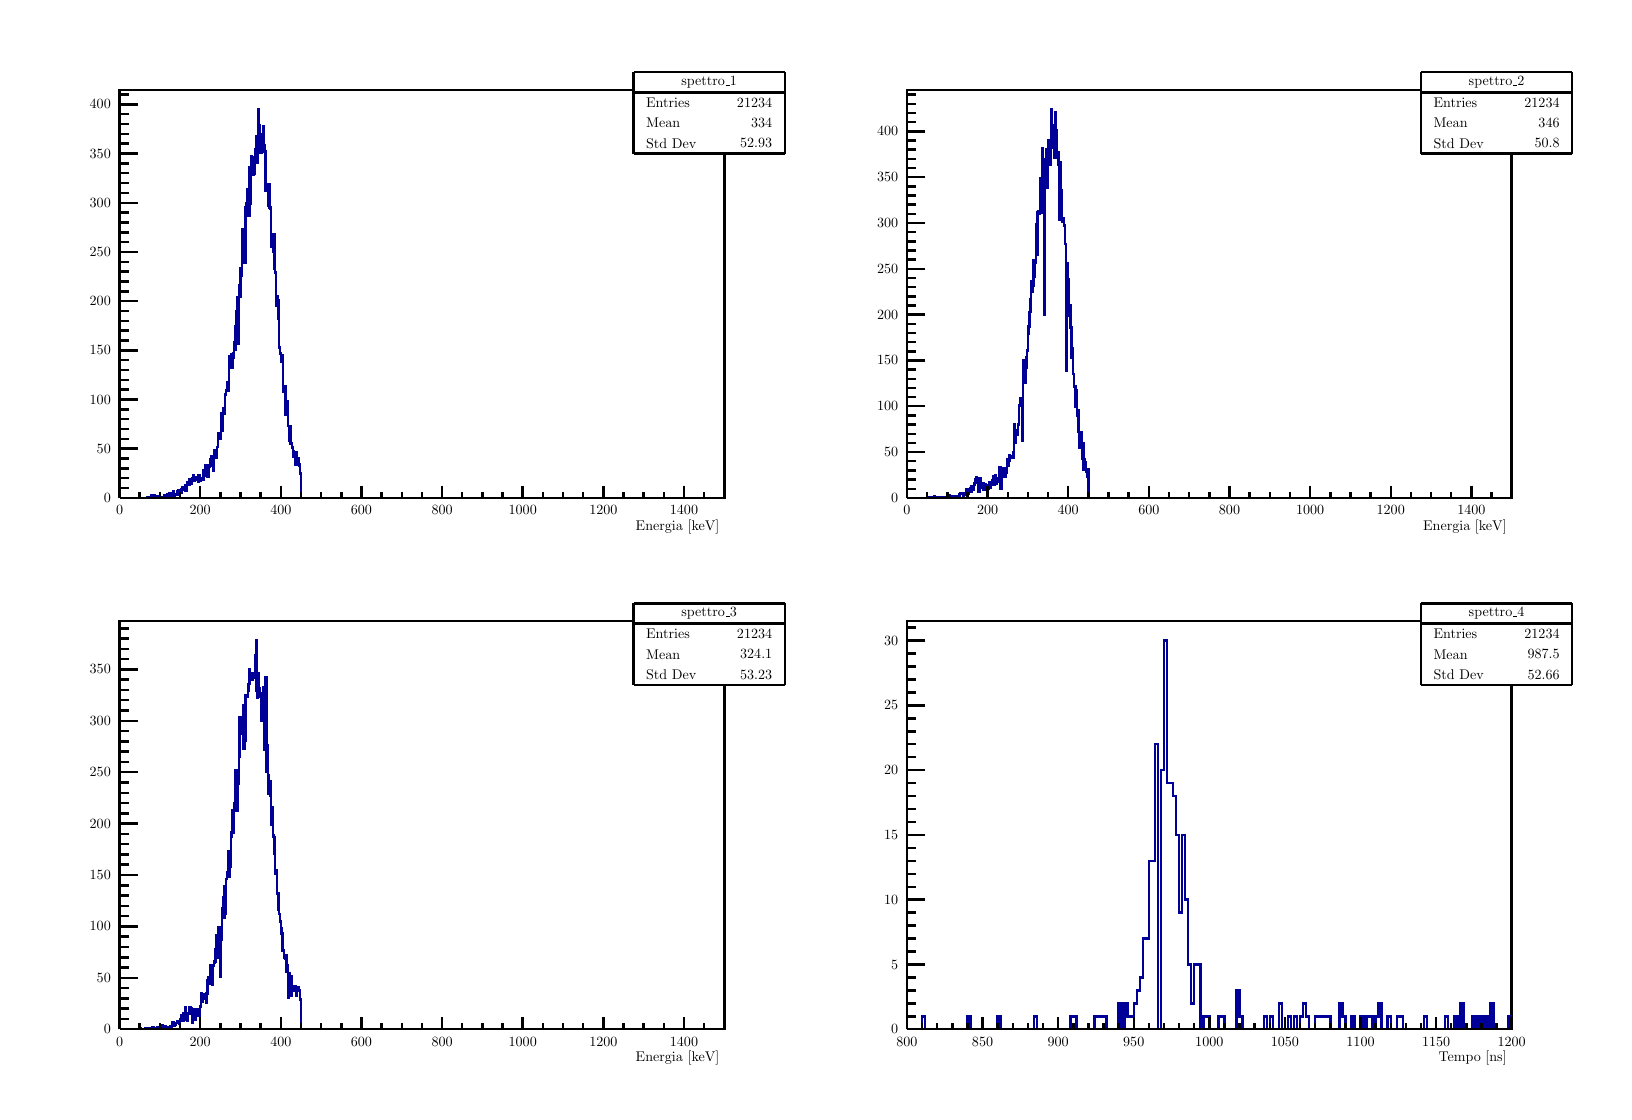
\begin{tikzpicture}
\pgfdeclareplotmark{cross} {
\pgfpathmoveto{\pgfpoint{-0.3\pgfplotmarksize}{\pgfplotmarksize}}
\pgfpathlineto{\pgfpoint{+0.3\pgfplotmarksize}{\pgfplotmarksize}}
\pgfpathlineto{\pgfpoint{+0.3\pgfplotmarksize}{0.3\pgfplotmarksize}}
\pgfpathlineto{\pgfpoint{+1\pgfplotmarksize}{0.3\pgfplotmarksize}}
\pgfpathlineto{\pgfpoint{+1\pgfplotmarksize}{-0.3\pgfplotmarksize}}
\pgfpathlineto{\pgfpoint{+0.3\pgfplotmarksize}{-0.3\pgfplotmarksize}}
\pgfpathlineto{\pgfpoint{+0.3\pgfplotmarksize}{-1.\pgfplotmarksize}}
\pgfpathlineto{\pgfpoint{-0.3\pgfplotmarksize}{-1.\pgfplotmarksize}}
\pgfpathlineto{\pgfpoint{-0.3\pgfplotmarksize}{-0.3\pgfplotmarksize}}
\pgfpathlineto{\pgfpoint{-1.\pgfplotmarksize}{-0.3\pgfplotmarksize}}
\pgfpathlineto{\pgfpoint{-1.\pgfplotmarksize}{0.3\pgfplotmarksize}}
\pgfpathlineto{\pgfpoint{-0.3\pgfplotmarksize}{0.3\pgfplotmarksize}}
\pgfpathclose
\pgfusepathqstroke
}
\pgfdeclareplotmark{cross*} {
\pgfpathmoveto{\pgfpoint{-0.3\pgfplotmarksize}{\pgfplotmarksize}}
\pgfpathlineto{\pgfpoint{+0.3\pgfplotmarksize}{\pgfplotmarksize}}
\pgfpathlineto{\pgfpoint{+0.3\pgfplotmarksize}{0.3\pgfplotmarksize}}
\pgfpathlineto{\pgfpoint{+1\pgfplotmarksize}{0.3\pgfplotmarksize}}
\pgfpathlineto{\pgfpoint{+1\pgfplotmarksize}{-0.3\pgfplotmarksize}}
\pgfpathlineto{\pgfpoint{+0.3\pgfplotmarksize}{-0.3\pgfplotmarksize}}
\pgfpathlineto{\pgfpoint{+0.3\pgfplotmarksize}{-1.\pgfplotmarksize}}
\pgfpathlineto{\pgfpoint{-0.3\pgfplotmarksize}{-1.\pgfplotmarksize}}
\pgfpathlineto{\pgfpoint{-0.3\pgfplotmarksize}{-0.3\pgfplotmarksize}}
\pgfpathlineto{\pgfpoint{-1.\pgfplotmarksize}{-0.3\pgfplotmarksize}}
\pgfpathlineto{\pgfpoint{-1.\pgfplotmarksize}{0.3\pgfplotmarksize}}
\pgfpathlineto{\pgfpoint{-0.3\pgfplotmarksize}{0.3\pgfplotmarksize}}
\pgfpathclose
\pgfusepathqfillstroke
}
\pgfdeclareplotmark{newstar} {
\pgfpathmoveto{\pgfqpoint{0pt}{\pgfplotmarksize}}
\pgfpathlineto{\pgfqpointpolar{44}{0.5\pgfplotmarksize}}
\pgfpathlineto{\pgfqpointpolar{18}{\pgfplotmarksize}}
\pgfpathlineto{\pgfqpointpolar{-20}{0.5\pgfplotmarksize}}
\pgfpathlineto{\pgfqpointpolar{-54}{\pgfplotmarksize}}
\pgfpathlineto{\pgfqpointpolar{-90}{0.5\pgfplotmarksize}}
\pgfpathlineto{\pgfqpointpolar{234}{\pgfplotmarksize}}
\pgfpathlineto{\pgfqpointpolar{198}{0.5\pgfplotmarksize}}
\pgfpathlineto{\pgfqpointpolar{162}{\pgfplotmarksize}}
\pgfpathlineto{\pgfqpointpolar{134}{0.5\pgfplotmarksize}}
\pgfpathclose
\pgfusepathqstroke
}
\pgfdeclareplotmark{newstar*} {
\pgfpathmoveto{\pgfqpoint{0pt}{\pgfplotmarksize}}
\pgfpathlineto{\pgfqpointpolar{44}{0.5\pgfplotmarksize}}
\pgfpathlineto{\pgfqpointpolar{18}{\pgfplotmarksize}}
\pgfpathlineto{\pgfqpointpolar{-20}{0.5\pgfplotmarksize}}
\pgfpathlineto{\pgfqpointpolar{-54}{\pgfplotmarksize}}
\pgfpathlineto{\pgfqpointpolar{-90}{0.5\pgfplotmarksize}}
\pgfpathlineto{\pgfqpointpolar{234}{\pgfplotmarksize}}
\pgfpathlineto{\pgfqpointpolar{198}{0.5\pgfplotmarksize}}
\pgfpathlineto{\pgfqpointpolar{162}{\pgfplotmarksize}}
\pgfpathlineto{\pgfqpointpolar{134}{0.5\pgfplotmarksize}}
\pgfpathclose
\pgfusepathqfillstroke
}
\definecolor{c}{rgb}{1,1,1};
\draw [color=c, fill=c] (0,0) rectangle (20,13.4957);
\draw [color=c, fill=c] (0.2,6.88281) rectangle (9.8,13.3607);
\draw [color=c, fill=c] (1.16,7.5306) rectangle (8.84,12.713);
\definecolor{c}{rgb}{0,0,0};
\draw [c,line width=0.9] (1.16,7.5306) -- (1.16,12.713) -- (8.84,12.713) -- (8.84,7.5306) -- (1.16,7.5306);
\definecolor{c}{rgb}{1,1,1};
\draw [color=c, fill=c] (1.16,7.5306) rectangle (8.84,12.713);
\definecolor{c}{rgb}{0,0,0};
\draw [c,line width=0.9] (1.16,7.5306) -- (1.16,12.713) -- (8.84,12.713) -- (8.84,7.5306) -- (1.16,7.5306);
\definecolor{c}{rgb}{0,0,0.6};
\draw [c,line width=0.9] (1.16,7.5306) -- (1.17024,7.5306) -- (1.17024,7.5306) -- (1.18048,7.5306) -- (1.18048,7.5306) -- (1.19072,7.5306) -- (1.19072,7.5306) -- (1.20096,7.5306) -- (1.20096,7.5306) -- (1.2112,7.5306) -- (1.2112,7.5306) --
 (1.22144,7.5306) -- (1.22144,7.5306) -- (1.23168,7.5306) -- (1.23168,7.5306) -- (1.24192,7.5306) -- (1.24192,7.5306) -- (1.25216,7.5306) -- (1.25216,7.5306) -- (1.2624,7.5306) -- (1.2624,7.5306) -- (1.27264,7.5306) -- (1.27264,7.5306) --
 (1.28288,7.5306) -- (1.28288,7.5306) -- (1.29312,7.5306) -- (1.29312,7.5306) -- (1.30336,7.5306) -- (1.30336,7.5306) -- (1.3136,7.5306) -- (1.3136,7.5306) -- (1.32384,7.5306) -- (1.32384,7.5306) -- (1.33408,7.5306) -- (1.33408,7.5306) --
 (1.34432,7.5306) -- (1.34432,7.5306) -- (1.35456,7.5306) -- (1.35456,7.5306) -- (1.3648,7.5306) -- (1.3648,7.5306) -- (1.37504,7.5306) -- (1.37504,7.5306) -- (1.38528,7.5306) -- (1.38528,7.5306) -- (1.39552,7.5306) -- (1.39552,7.5306) --
 (1.40576,7.5306) -- (1.40576,7.5306) -- (1.416,7.5306) -- (1.416,7.5306) -- (1.42624,7.5306) -- (1.42624,7.5306) -- (1.43648,7.5306) -- (1.43648,7.5306) -- (1.44672,7.5306) -- (1.44672,7.5306) -- (1.45696,7.5306) -- (1.45696,7.5306) --
 (1.4672,7.5306) -- (1.4672,7.5306) -- (1.47744,7.5306) -- (1.47744,7.5306) -- (1.48768,7.5306) -- (1.48768,7.5306) -- (1.49792,7.5306) -- (1.49792,7.5306) -- (1.50816,7.5306) -- (1.50816,7.5431) -- (1.5184,7.5431) -- (1.5184,7.5431) --
 (1.52864,7.5431) -- (1.52864,7.5431) -- (1.53888,7.5431) -- (1.53888,7.5306) -- (1.54912,7.5306) -- (1.54912,7.5431) -- (1.55936,7.5431) -- (1.55936,7.56809) -- (1.5696,7.56809) -- (1.5696,7.55559) -- (1.57984,7.55559) -- (1.57984,7.5306) --
 (1.59008,7.5306) -- (1.59008,7.56809) -- (1.60032,7.56809) -- (1.60032,7.56809) -- (1.61056,7.56809) -- (1.61056,7.5306) -- (1.6208,7.5306) -- (1.6208,7.5431) -- (1.63104,7.5431) -- (1.63104,7.55559) -- (1.64128,7.55559) -- (1.64128,7.5306) --
 (1.65152,7.5306) -- (1.65152,7.5431) -- (1.66176,7.5431) -- (1.66176,7.5431) -- (1.672,7.5431) -- (1.672,7.5306) -- (1.68224,7.5306) -- (1.68224,7.5431) -- (1.69248,7.5431) -- (1.69248,7.5431) -- (1.70272,7.5431) -- (1.70272,7.5306) --
 (1.71296,7.5306) -- (1.71296,7.5431) -- (1.7232,7.5431) -- (1.7232,7.56809) -- (1.73344,7.56809) -- (1.73344,7.55559) -- (1.74368,7.55559) -- (1.74368,7.55559) -- (1.75392,7.55559) -- (1.75392,7.5431) -- (1.76416,7.5431) -- (1.76416,7.58058) --
 (1.7744,7.58058) -- (1.7744,7.5431) -- (1.78464,7.5431) -- (1.78464,7.58058) -- (1.79488,7.58058) -- (1.79488,7.59308) -- (1.80512,7.59308) -- (1.80512,7.55559) -- (1.81536,7.55559) -- (1.81536,7.58058) -- (1.8256,7.58058) -- (1.8256,7.5306) --
 (1.83584,7.5306) -- (1.83584,7.61807) -- (1.84608,7.61807) -- (1.84608,7.58058) -- (1.85632,7.58058) -- (1.85632,7.55559) -- (1.86656,7.55559) -- (1.86656,7.58058) -- (1.8768,7.58058) -- (1.8768,7.56809) -- (1.88704,7.56809) -- (1.88704,7.58058) --
 (1.89728,7.58058) -- (1.89728,7.61807) -- (1.90752,7.61807) -- (1.90752,7.63056) -- (1.91776,7.63056) -- (1.91776,7.56809) -- (1.928,7.56809) -- (1.928,7.60557) -- (1.93824,7.60557) -- (1.93824,7.59308) -- (1.94848,7.59308) -- (1.94848,7.64306) --
 (1.95872,7.64306) -- (1.95872,7.66805) -- (1.96896,7.66805) -- (1.96896,7.63056) -- (1.9792,7.63056) -- (1.9792,7.63056) -- (1.98944,7.63056) -- (1.98944,7.69304) -- (1.99968,7.69304) -- (1.99968,7.61807) -- (2.00992,7.61807) -- (2.00992,7.69304) --
 (2.02016,7.69304) -- (2.02016,7.73052) -- (2.0304,7.73052) -- (2.0304,7.70553) -- (2.04064,7.70553) -- (2.04064,7.69304) -- (2.05088,7.69304) -- (2.05088,7.76801) -- (2.06112,7.76801) -- (2.06112,7.70553) -- (2.07136,7.70553) -- (2.07136,7.75551) --
 (2.0816,7.75551) -- (2.0816,7.7805) -- (2.09184,7.7805) -- (2.09184,7.81799) -- (2.10208,7.81799) -- (2.10208,7.74302) -- (2.11232,7.74302) -- (2.11232,7.7805) -- (2.12256,7.7805) -- (2.12256,7.75551) -- (2.1328,7.75551) -- (2.1328,7.793) --
 (2.14304,7.793) -- (2.14304,7.76801) -- (2.15328,7.76801) -- (2.15328,7.73052) -- (2.16352,7.73052) -- (2.16352,7.81799) -- (2.17376,7.81799) -- (2.17376,7.7805) -- (2.184,7.7805) -- (2.184,7.74302) -- (2.19424,7.74302) -- (2.19424,7.76801) --
 (2.20448,7.76801) -- (2.20448,7.7805) -- (2.21472,7.7805) -- (2.21472,7.75551) -- (2.22496,7.75551) -- (2.22496,7.88047) -- (2.2352,7.88047) -- (2.2352,7.84298) -- (2.24544,7.84298) -- (2.24544,7.94294) -- (2.25568,7.94294) -- (2.25568,7.81799) --
 (2.26592,7.81799) -- (2.26592,7.90546) -- (2.27616,7.90546) -- (2.27616,7.80549) -- (2.2864,7.80549) -- (2.2864,7.94294) -- (2.29664,7.94294) -- (2.29664,7.93045) -- (2.30688,7.93045) -- (2.30688,7.95544) -- (2.31712,7.95544) -- (2.31712,8.01791) --
 (2.32736,8.01791) -- (2.32736,8.0554) -- (2.3376,8.0554) -- (2.3376,7.94294) -- (2.34784,7.94294) -- (2.34784,7.88047) -- (2.35808,7.88047) -- (2.35808,8.08039) -- (2.36832,8.08039) -- (2.36832,8.13037) -- (2.37856,8.13037) -- (2.37856,8.11787) --
 (2.3888,8.11787) -- (2.3888,8.0429) -- (2.39904,8.0429) -- (2.39904,8.18035) -- (2.40928,8.18035) -- (2.40928,8.35528) -- (2.41952,8.35528) -- (2.41952,8.28031) -- (2.42976,8.28031) -- (2.42976,8.33029) -- (2.44,8.33029) -- (2.44,8.28031) --
 (2.45024,8.28031) -- (2.45024,8.60518) -- (2.46048,8.60518) -- (2.46048,8.38027) -- (2.47072,8.38027) -- (2.47072,8.66766) -- (2.48096,8.66766) -- (2.48096,8.63017) -- (2.4912,8.63017) -- (2.4912,8.60518) -- (2.50144,8.60518) -- (2.50144,8.84259) --
 (2.51168,8.84259) -- (2.51168,8.89257) -- (2.52192,8.89257) -- (2.52192,8.93005) -- (2.53216,8.93005) -- (2.53216,9.00502) -- (2.5424,9.00502) -- (2.5424,8.89257) -- (2.55264,8.89257) -- (2.55264,9.3299) -- (2.56288,9.3299) -- (2.56288,9.30491) --
 (2.57312,9.30491) -- (2.57312,9.35489) -- (2.58336,9.35489) -- (2.58336,9.17996) -- (2.5936,9.17996) -- (2.5936,9.30491) -- (2.60384,9.30491) -- (2.60384,9.36738) -- (2.61408,9.36738) -- (2.61408,9.50483) -- (2.62432,9.50483) -- (2.62432,9.41736) --
 (2.63456,9.41736) -- (2.63456,9.70475) -- (2.6448,9.70475) -- (2.6448,9.90467) -- (2.65504,9.90467) -- (2.65504,10.0796) -- (2.66528,10.0796) -- (2.66528,9.49234) -- (2.67552,9.49234) -- (2.67552,10.2295) -- (2.68576,10.2295) -- (2.68576,10.0796) --
 (2.696,10.0796) -- (2.696,10.442) -- (2.70624,10.442) -- (2.70624,10.3545) -- (2.71648,10.3545) -- (2.71648,10.9418) -- (2.72672,10.9418) -- (2.72672,10.6169) -- (2.73696,10.6169) -- (2.73696,10.8293) -- (2.7472,10.8293) -- (2.7472,10.5169) --
 (2.75744,10.5169) -- (2.75744,11.2167) -- (2.76768,11.2167) -- (2.76768,11.2666) -- (2.77792,11.2666) -- (2.77792,11.4541) -- (2.78816,11.4541) -- (2.78816,11.2916) -- (2.7984,11.2916) -- (2.7984,11.1167) -- (2.80864,11.1167) -- (2.80864,11.729) --
 (2.81888,11.729) -- (2.81888,11.2666) -- (2.82912,11.2666) -- (2.82912,11.8664) -- (2.83936,11.8664) -- (2.83936,11.729) -- (2.8496,11.729) -- (2.8496,11.629) -- (2.85984,11.629) -- (2.85984,11.8539) -- (2.87008,11.8539) -- (2.87008,11.6415) --
 (2.88032,11.6415) -- (2.88032,11.9539) -- (2.89056,11.9539) -- (2.89056,12.1288) -- (2.9008,12.1288) -- (2.9008,11.9664) -- (2.91104,11.9664) -- (2.91104,11.7914) -- (2.92128,11.7914) -- (2.92128,12.4662) -- (2.93152,12.4662) -- (2.93152,12.2663) --
 (2.94176,12.2663) -- (2.94176,12.1288) -- (2.952,12.1288) -- (2.952,11.9164) -- (2.96224,11.9164) -- (2.96224,12.1538) -- (2.97248,12.1538) -- (2.97248,12.0413) -- (2.98272,12.0413) -- (2.98272,12.2538) -- (2.99296,12.2538) -- (2.99296,12.0039) --
 (3.0032,12.0039) -- (3.0032,11.9289) -- (3.01344,11.9289) -- (3.01344,11.4291) -- (3.02368,11.4291) -- (3.02368,11.4916) -- (3.03392,11.4916) -- (3.03392,11.5165) -- (3.04416,11.5165) -- (3.04416,11.2417) -- (3.0544,11.2417) -- (3.0544,11.5165) --
 (3.06464,11.5165) -- (3.06464,11.2167) -- (3.07488,11.2167) -- (3.07488,11.2042) -- (3.08512,11.2042) -- (3.08512,10.7169) -- (3.09536,10.7169) -- (3.09536,10.7294) -- (3.1056,10.7294) -- (3.1056,10.6544) -- (3.11584,10.6544) -- (3.11584,10.8793) --
 (3.12608,10.8793) -- (3.12608,10.442) -- (3.13632,10.442) -- (3.13632,10.392) -- (3.14656,10.392) -- (3.14656,9.96715) -- (3.1568,9.96715) -- (3.1568,10.0921) -- (3.16704,10.0921) -- (3.16704,10.0421) -- (3.17728,10.0421) -- (3.17728,9.80471) --
 (3.18752,9.80471) -- (3.18752,9.44235) -- (3.19776,9.44235) -- (3.19776,9.36738) -- (3.208,9.36738) -- (3.208,9.25493) -- (3.21824,9.25493) -- (3.21824,9.34239) -- (3.22848,9.34239) -- (3.22848,9.30491) -- (3.23872,9.30491) -- (3.23872,8.88007) --
 (3.24896,8.88007) -- (3.24896,8.94255) -- (3.2592,8.94255) -- (3.2592,8.95504) -- (3.26944,8.95504) -- (3.26944,8.59269) -- (3.27968,8.59269) -- (3.27968,8.75512) -- (3.28992,8.75512) -- (3.28992,8.59269) -- (3.30016,8.59269) -- (3.30016,8.44275) --
 (3.3104,8.44275) -- (3.3104,8.25532) -- (3.32064,8.25532) -- (3.32064,8.44275) -- (3.33088,8.44275) -- (3.33088,8.21783) -- (3.34112,8.21783) -- (3.34112,8.23033) -- (3.35136,8.23033) -- (3.35136,8.16785) -- (3.3616,8.16785) -- (3.3616,8.11787) --
 (3.37184,8.11787) -- (3.37184,8.0554) -- (3.38208,8.0554) -- (3.38208,8.09288) -- (3.39232,8.09288) -- (3.39232,7.95544) -- (3.40256,7.95544) -- (3.40256,8.10538) -- (3.4128,8.10538) -- (3.4128,7.99292) -- (3.42304,7.99292) -- (3.42304,8.03041) --
 (3.43328,8.03041) -- (3.43328,7.95544) -- (3.44352,7.95544) -- (3.44352,7.94294) -- (3.45376,7.94294) -- (3.45376,7.84298) -- (3.464,7.84298) -- (3.464,7.5306) -- (3.47424,7.5306) -- (3.47424,7.5306) -- (3.48448,7.5306) -- (3.48448,7.5306) --
 (3.49472,7.5306) -- (3.49472,7.5306) -- (3.50496,7.5306) -- (3.50496,7.5306) -- (3.5152,7.5306) -- (3.5152,7.5306) -- (3.52544,7.5306) -- (3.52544,7.5306) -- (3.53568,7.5306) -- (3.53568,7.5306) -- (3.54592,7.5306) -- (3.54592,7.5306) --
 (3.55616,7.5306) -- (3.55616,7.5306) -- (3.5664,7.5306) -- (3.5664,7.5306) -- (3.57664,7.5306) -- (3.57664,7.5306) -- (3.58688,7.5306) -- (3.58688,7.5306) -- (3.59712,7.5306) -- (3.59712,7.5306) -- (3.60736,7.5306) -- (3.60736,7.5306) --
 (3.6176,7.5306) -- (3.6176,7.5306) -- (3.62784,7.5306) -- (3.62784,7.5306) -- (3.63808,7.5306) -- (3.63808,7.5306) -- (3.64832,7.5306) -- (3.64832,7.5306) -- (3.65856,7.5306) -- (3.65856,7.5306) -- (3.6688,7.5306) -- (3.6688,7.5306) --
 (3.67904,7.5306) -- (3.67904,7.5306) -- (3.68928,7.5306) -- (3.68928,7.5306) -- (3.69952,7.5306) -- (3.69952,7.5306) -- (3.70976,7.5306) -- (3.70976,7.5306) -- (3.72,7.5306) -- (3.72,7.5306) -- (3.73024,7.5306) -- (3.73024,7.5306) --
 (3.74048,7.5306) -- (3.74048,7.5306) -- (3.75072,7.5306) -- (3.75072,7.5306) -- (3.76096,7.5306) -- (3.76096,7.5306) -- (3.7712,7.5306) -- (3.7712,7.5306) -- (3.78144,7.5306) -- (3.78144,7.5306) -- (3.79168,7.5306) -- (3.79168,7.5306) --
 (3.80192,7.5306) -- (3.80192,7.5306) -- (3.81216,7.5306) -- (3.81216,7.5306) -- (3.8224,7.5306) -- (3.8224,7.5306) -- (3.83264,7.5306) -- (3.83264,7.5306) -- (3.84288,7.5306) -- (3.84288,7.5306) -- (3.85312,7.5306) -- (3.85312,7.5306) --
 (3.86336,7.5306) -- (3.86336,7.5306) -- (3.8736,7.5306) -- (3.8736,7.5306) -- (3.88384,7.5306) -- (3.88384,7.5306) -- (3.89408,7.5306) -- (3.89408,7.5306) -- (3.90432,7.5306) -- (3.90432,7.5306) -- (3.91456,7.5306) -- (3.91456,7.5306) --
 (3.9248,7.5306) -- (3.9248,7.5306) -- (3.93504,7.5306) -- (3.93504,7.5306) -- (3.94528,7.5306) -- (3.94528,7.5306) -- (3.95552,7.5306) -- (3.95552,7.5306) -- (3.96576,7.5306) -- (3.96576,7.5306) -- (3.976,7.5306) -- (3.976,7.5306) --
 (3.98624,7.5306) -- (3.98624,7.5306) -- (3.99648,7.5306) -- (3.99648,7.5306) -- (4.00672,7.5306) -- (4.00672,7.5306) -- (4.01696,7.5306) -- (4.01696,7.5306) -- (4.0272,7.5306) -- (4.0272,7.5306) -- (4.03744,7.5306) -- (4.03744,7.5306) --
 (4.04768,7.5306) -- (4.04768,7.5306) -- (4.05792,7.5306) -- (4.05792,7.5306) -- (4.06816,7.5306) -- (4.06816,7.5306) -- (4.0784,7.5306) -- (4.0784,7.5306) -- (4.08864,7.5306) -- (4.08864,7.5306) -- (4.09888,7.5306) -- (4.09888,7.5306) --
 (4.10912,7.5306) -- (4.10912,7.5306) -- (4.11936,7.5306) -- (4.11936,7.5306) -- (4.1296,7.5306) -- (4.1296,7.5306) -- (4.13984,7.5306) -- (4.13984,7.5306) -- (4.15008,7.5306) -- (4.15008,7.5306) -- (4.16032,7.5306) -- (4.16032,7.5306) --
 (4.17056,7.5306) -- (4.17056,7.5306) -- (4.1808,7.5306) -- (4.1808,7.5306) -- (4.19104,7.5306) -- (4.19104,7.5306) -- (4.20128,7.5306) -- (4.20128,7.5306) -- (4.21152,7.5306) -- (4.21152,7.5306) -- (4.22176,7.5306) -- (4.22176,7.5306) --
 (4.232,7.5306) -- (4.232,7.5306) -- (4.24224,7.5306) -- (4.24224,7.5306) -- (4.25248,7.5306) -- (4.25248,7.5306) -- (4.26272,7.5306) -- (4.26272,7.5306) -- (4.27296,7.5306) -- (4.27296,7.5306) -- (4.2832,7.5306) -- (4.2832,7.5306) --
 (4.29344,7.5306) -- (4.29344,7.5306) -- (4.30368,7.5306) -- (4.30368,7.5306) -- (4.31392,7.5306) -- (4.31392,7.5306) -- (4.32416,7.5306) -- (4.32416,7.5306) -- (4.3344,7.5306) -- (4.3344,7.5306) -- (4.34464,7.5306) -- (4.34464,7.5306) --
 (4.35488,7.5306) -- (4.35488,7.5306) -- (4.36512,7.5306) -- (4.36512,7.5306) -- (4.37536,7.5306) -- (4.37536,7.5306) -- (4.3856,7.5306) -- (4.3856,7.5306) -- (4.39584,7.5306) -- (4.39584,7.5306) -- (4.40608,7.5306) -- (4.40608,7.5306) --
 (4.41632,7.5306) -- (4.41632,7.5306) -- (4.42656,7.5306) -- (4.42656,7.5306) -- (4.4368,7.5306) -- (4.4368,7.5306) -- (4.44704,7.5306) -- (4.44704,7.5306) -- (4.45728,7.5306) -- (4.45728,7.5306) -- (4.46752,7.5306) -- (4.46752,7.5306) --
 (4.47776,7.5306) -- (4.47776,7.5306) -- (4.488,7.5306) -- (4.488,7.5306) -- (4.49824,7.5306) -- (4.49824,7.5306) -- (4.50848,7.5306) -- (4.50848,7.5306) -- (4.51872,7.5306) -- (4.51872,7.5306) -- (4.52896,7.5306) -- (4.52896,7.5306) --
 (4.5392,7.5306) -- (4.5392,7.5306) -- (4.54944,7.5306) -- (4.54944,7.5306) -- (4.55968,7.5306) -- (4.55968,7.5306) -- (4.56992,7.5306) -- (4.56992,7.5306) -- (4.58016,7.5306) -- (4.58016,7.5306) -- (4.5904,7.5306) -- (4.5904,7.5306) --
 (4.60064,7.5306) -- (4.60064,7.5306) -- (4.61088,7.5306) -- (4.61088,7.5306) -- (4.62112,7.5306) -- (4.62112,7.5306) -- (4.63136,7.5306) -- (4.63136,7.5306) -- (4.6416,7.5306) -- (4.6416,7.5306) -- (4.65184,7.5306) -- (4.65184,7.5306) --
 (4.66208,7.5306) -- (4.66208,7.5306) -- (4.67232,7.5306) -- (4.67232,7.5306) -- (4.68256,7.5306) -- (4.68256,7.5306) -- (4.6928,7.5306) -- (4.6928,7.5306) -- (4.70304,7.5306) -- (4.70304,7.5306) -- (4.71328,7.5306) -- (4.71328,7.5306) --
 (4.72352,7.5306) -- (4.72352,7.5306) -- (4.73376,7.5306) -- (4.73376,7.5306) -- (4.744,7.5306) -- (4.744,7.5306) -- (4.75424,7.5306) -- (4.75424,7.5306) -- (4.76448,7.5306) -- (4.76448,7.5306) -- (4.77472,7.5306) -- (4.77472,7.5306) --
 (4.78496,7.5306) -- (4.78496,7.5306) -- (4.7952,7.5306) -- (4.7952,7.5306) -- (4.80544,7.5306) -- (4.80544,7.5306) -- (4.81568,7.5306) -- (4.81568,7.5306) -- (4.82592,7.5306) -- (4.82592,7.5306) -- (4.83616,7.5306) -- (4.83616,7.5306) --
 (4.8464,7.5306) -- (4.8464,7.5306) -- (4.85664,7.5306) -- (4.85664,7.5306) -- (4.86688,7.5306) -- (4.86688,7.5306) -- (4.87712,7.5306) -- (4.87712,7.5306) -- (4.88736,7.5306) -- (4.88736,7.5306) -- (4.8976,7.5306) -- (4.8976,7.5306) --
 (4.90784,7.5306) -- (4.90784,7.5306) -- (4.91808,7.5306) -- (4.91808,7.5306) -- (4.92832,7.5306) -- (4.92832,7.5306) -- (4.93856,7.5306) -- (4.93856,7.5306) -- (4.9488,7.5306) -- (4.9488,7.5306) -- (4.95904,7.5306) -- (4.95904,7.5306) --
 (4.96928,7.5306) -- (4.96928,7.5306) -- (4.97952,7.5306) -- (4.97952,7.5306) -- (4.98976,7.5306) -- (4.98976,7.5306) -- (5,7.5306) -- (5,7.5306) -- (5.01024,7.5306) -- (5.01024,7.5306) -- (5.02048,7.5306) -- (5.02048,7.5306) -- (5.03072,7.5306) --
 (5.03072,7.5306) -- (5.04096,7.5306) -- (5.04096,7.5306) -- (5.0512,7.5306) -- (5.0512,7.5306) -- (5.06144,7.5306) -- (5.06144,7.5306) -- (5.07168,7.5306) -- (5.07168,7.5306) -- (5.08192,7.5306) -- (5.08192,7.5306) -- (5.09216,7.5306) --
 (5.09216,7.5306) -- (5.1024,7.5306) -- (5.1024,7.5306) -- (5.11264,7.5306) -- (5.11264,7.5306) -- (5.12288,7.5306) -- (5.12288,7.5306) -- (5.13312,7.5306) -- (5.13312,7.5306) -- (5.14336,7.5306) -- (5.14336,7.5306) -- (5.1536,7.5306) --
 (5.1536,7.5306) -- (5.16384,7.5306) -- (5.16384,7.5306) -- (5.17408,7.5306) -- (5.17408,7.5306) -- (5.18432,7.5306) -- (5.18432,7.5306) -- (5.19456,7.5306) -- (5.19456,7.5306) -- (5.2048,7.5306) -- (5.2048,7.5306) -- (5.21504,7.5306) --
 (5.21504,7.5306) -- (5.22528,7.5306) -- (5.22528,7.5306) -- (5.23552,7.5306) -- (5.23552,7.5306) -- (5.24576,7.5306) -- (5.24576,7.5306) -- (5.256,7.5306) -- (5.256,7.5306) -- (5.26624,7.5306) -- (5.26624,7.5306) -- (5.27648,7.5306) --
 (5.27648,7.5306) -- (5.28672,7.5306) -- (5.28672,7.5306) -- (5.29696,7.5306) -- (5.29696,7.5306) -- (5.3072,7.5306) -- (5.3072,7.5306) -- (5.31744,7.5306) -- (5.31744,7.5306) -- (5.32768,7.5306) -- (5.32768,7.5306) -- (5.33792,7.5306) --
 (5.33792,7.5306) -- (5.34816,7.5306) -- (5.34816,7.5306) -- (5.3584,7.5306) -- (5.3584,7.5306) -- (5.36864,7.5306) -- (5.36864,7.5306) -- (5.37888,7.5306) -- (5.37888,7.5306) -- (5.38912,7.5306) -- (5.38912,7.5306) -- (5.39936,7.5306) --
 (5.39936,7.5306) -- (5.4096,7.5306) -- (5.4096,7.5306) -- (5.41984,7.5306) -- (5.41984,7.5306) -- (5.43008,7.5306) -- (5.43008,7.5306) -- (5.44032,7.5306) -- (5.44032,7.5306) -- (5.45056,7.5306) -- (5.45056,7.5306) -- (5.4608,7.5306) --
 (5.4608,7.5306) -- (5.47104,7.5306) -- (5.47104,7.5306) -- (5.48128,7.5306) -- (5.48128,7.5306) -- (5.49152,7.5306) -- (5.49152,7.5306) -- (5.50176,7.5306) -- (5.50176,7.5306) -- (5.512,7.5306) -- (5.512,7.5306) -- (5.52224,7.5306) --
 (5.52224,7.5306) -- (5.53248,7.5306) -- (5.53248,7.5306) -- (5.54272,7.5306) -- (5.54272,7.5306) -- (5.55296,7.5306) -- (5.55296,7.5306) -- (5.5632,7.5306) -- (5.5632,7.5306) -- (5.57344,7.5306) -- (5.57344,7.5306) -- (5.58368,7.5306) --
 (5.58368,7.5306) -- (5.59392,7.5306) -- (5.59392,7.5306) -- (5.60416,7.5306) -- (5.60416,7.5306) -- (5.6144,7.5306) -- (5.6144,7.5306) -- (5.62464,7.5306) -- (5.62464,7.5306) -- (5.63488,7.5306) -- (5.63488,7.5306) -- (5.64512,7.5306) --
 (5.64512,7.5306) -- (5.65536,7.5306) -- (5.65536,7.5306) -- (5.6656,7.5306) -- (5.6656,7.5306) -- (5.67584,7.5306) -- (5.67584,7.5306) -- (5.68608,7.5306) -- (5.68608,7.5306) -- (5.69632,7.5306) -- (5.69632,7.5306) -- (5.70656,7.5306) --
 (5.70656,7.5306) -- (5.7168,7.5306) -- (5.7168,7.5306) -- (5.72704,7.5306) -- (5.72704,7.5306) -- (5.73728,7.5306) -- (5.73728,7.5306) -- (5.74752,7.5306) -- (5.74752,7.5306) -- (5.75776,7.5306) -- (5.75776,7.5306) -- (5.768,7.5306) --
 (5.768,7.5306) -- (5.77824,7.5306) -- (5.77824,7.5306) -- (5.78848,7.5306) -- (5.78848,7.5306) -- (5.79872,7.5306) -- (5.79872,7.5306) -- (5.80896,7.5306) -- (5.80896,7.5306) -- (5.8192,7.5306) -- (5.8192,7.5306) -- (5.82944,7.5306) --
 (5.82944,7.5306) -- (5.83968,7.5306) -- (5.83968,7.5306) -- (5.84992,7.5306) -- (5.84992,7.5306) -- (5.86016,7.5306) -- (5.86016,7.5306) -- (5.8704,7.5306) -- (5.8704,7.5306) -- (5.88064,7.5306) -- (5.88064,7.5306) -- (5.89088,7.5306) --
 (5.89088,7.5306) -- (5.90112,7.5306) -- (5.90112,7.5306) -- (5.91136,7.5306) -- (5.91136,7.5306) -- (5.9216,7.5306) -- (5.9216,7.5306) -- (5.93184,7.5306) -- (5.93184,7.5306) -- (5.94208,7.5306) -- (5.94208,7.5306) -- (5.95232,7.5306) --
 (5.95232,7.5306) -- (5.96256,7.5306) -- (5.96256,7.5306) -- (5.9728,7.5306) -- (5.9728,7.5306) -- (5.98304,7.5306) -- (5.98304,7.5306) -- (5.99328,7.5306) -- (5.99328,7.5306) -- (6.00352,7.5306) -- (6.00352,7.5306) -- (6.01376,7.5306) --
 (6.01376,7.5306) -- (6.024,7.5306) -- (6.024,7.5306) -- (6.03424,7.5306) -- (6.03424,7.5306) -- (6.04448,7.5306) -- (6.04448,7.5306) -- (6.05472,7.5306) -- (6.05472,7.5306) -- (6.06496,7.5306) -- (6.06496,7.5306) -- (6.0752,7.5306) --
 (6.0752,7.5306) -- (6.08544,7.5306) -- (6.08544,7.5306) -- (6.09568,7.5306) -- (6.09568,7.5306) -- (6.10592,7.5306) -- (6.10592,7.5306) -- (6.11616,7.5306) -- (6.11616,7.5306) -- (6.1264,7.5306) -- (6.1264,7.5306) -- (6.13664,7.5306) --
 (6.13664,7.5306) -- (6.14688,7.5306) -- (6.14688,7.5306) -- (6.15712,7.5306) -- (6.15712,7.5306) -- (6.16736,7.5306) -- (6.16736,7.5306) -- (6.1776,7.5306) -- (6.1776,7.5306) -- (6.18784,7.5306) -- (6.18784,7.5306) -- (6.19808,7.5306) --
 (6.19808,7.5306) -- (6.20832,7.5306) -- (6.20832,7.5306) -- (6.21856,7.5306) -- (6.21856,7.5306) -- (6.2288,7.5306) -- (6.2288,7.5306) -- (6.23904,7.5306) -- (6.23904,7.5306) -- (6.24928,7.5306) -- (6.24928,7.5306) -- (6.25952,7.5306) --
 (6.25952,7.5306) -- (6.26976,7.5306) -- (6.26976,7.5306) -- (6.28,7.5306) -- (6.28,7.5306) -- (6.29024,7.5306) -- (6.29024,7.5306) -- (6.30048,7.5306) -- (6.30048,7.5306) -- (6.31072,7.5306) -- (6.31072,7.5306) -- (6.32096,7.5306) --
 (6.32096,7.5306) -- (6.3312,7.5306) -- (6.3312,7.5306) -- (6.34144,7.5306) -- (6.34144,7.5306) -- (6.35168,7.5306) -- (6.35168,7.5306) -- (6.36192,7.5306) -- (6.36192,7.5306) -- (6.37216,7.5306) -- (6.37216,7.5306) -- (6.3824,7.5306) --
 (6.3824,7.5306) -- (6.39264,7.5306) -- (6.39264,7.5306) -- (6.40288,7.5306) -- (6.40288,7.5306) -- (6.41312,7.5306) -- (6.41312,7.5306) -- (6.42336,7.5306) -- (6.42336,7.5306) -- (6.4336,7.5306) -- (6.4336,7.5306) -- (6.44384,7.5306) --
 (6.44384,7.5306) -- (6.45408,7.5306) -- (6.45408,7.5306) -- (6.46432,7.5306) -- (6.46432,7.5306) -- (6.47456,7.5306) -- (6.47456,7.5306) -- (6.4848,7.5306) -- (6.4848,7.5306) -- (6.49504,7.5306) -- (6.49504,7.5306) -- (6.50528,7.5306) --
 (6.50528,7.5306) -- (6.51552,7.5306) -- (6.51552,7.5306) -- (6.52576,7.5306) -- (6.52576,7.5306) -- (6.536,7.5306) -- (6.536,7.5306) -- (6.54624,7.5306) -- (6.54624,7.5306) -- (6.55648,7.5306) -- (6.55648,7.5306) -- (6.56672,7.5306) --
 (6.56672,7.5306) -- (6.57696,7.5306) -- (6.57696,7.5306) -- (6.5872,7.5306) -- (6.5872,7.5306) -- (6.59744,7.5306) -- (6.59744,7.5306) -- (6.60768,7.5306) -- (6.60768,7.5306) -- (6.61792,7.5306) -- (6.61792,7.5306) -- (6.62816,7.5306) --
 (6.62816,7.5306) -- (6.6384,7.5306) -- (6.6384,7.5306) -- (6.64864,7.5306) -- (6.64864,7.5306) -- (6.65888,7.5306) -- (6.65888,7.5306) -- (6.66912,7.5306) -- (6.66912,7.5306) -- (6.67936,7.5306) -- (6.67936,7.5306) -- (6.6896,7.5306) --
 (6.6896,7.5306) -- (6.69984,7.5306) -- (6.69984,7.5306) -- (6.71008,7.5306) -- (6.71008,7.5306) -- (6.72032,7.5306) -- (6.72032,7.5306) -- (6.73056,7.5306) -- (6.73056,7.5306) -- (6.7408,7.5306) -- (6.7408,7.5306) -- (6.75104,7.5306) --
 (6.75104,7.5306) -- (6.76128,7.5306) -- (6.76128,7.5306) -- (6.77152,7.5306) -- (6.77152,7.5306) -- (6.78176,7.5306) -- (6.78176,7.5306) -- (6.792,7.5306) -- (6.792,7.5306) -- (6.80224,7.5306) -- (6.80224,7.5306) -- (6.81248,7.5306) --
 (6.81248,7.5306) -- (6.82272,7.5306) -- (6.82272,7.5306) -- (6.83296,7.5306) -- (6.83296,7.5306) -- (6.8432,7.5306) -- (6.8432,7.5306) -- (6.85344,7.5306) -- (6.85344,7.5306) -- (6.86368,7.5306) -- (6.86368,7.5306) -- (6.87392,7.5306) --
 (6.87392,7.5306) -- (6.88416,7.5306) -- (6.88416,7.5306) -- (6.8944,7.5306) -- (6.8944,7.5306) -- (6.90464,7.5306) -- (6.90464,7.5306) -- (6.91488,7.5306) -- (6.91488,7.5306) -- (6.92512,7.5306) -- (6.92512,7.5306) -- (6.93536,7.5306) --
 (6.93536,7.5306) -- (6.9456,7.5306) -- (6.9456,7.5306) -- (6.95584,7.5306) -- (6.95584,7.5306) -- (6.96608,7.5306) -- (6.96608,7.5306) -- (6.97632,7.5306) -- (6.97632,7.5306) -- (6.98656,7.5306) -- (6.98656,7.5306) -- (6.9968,7.5306) --
 (6.9968,7.5306) -- (7.00704,7.5306) -- (7.00704,7.5306) -- (7.01728,7.5306) -- (7.01728,7.5306) -- (7.02752,7.5306) -- (7.02752,7.5306) -- (7.03776,7.5306) -- (7.03776,7.5306) -- (7.048,7.5306) -- (7.048,7.5306) -- (7.05824,7.5306) --
 (7.05824,7.5306) -- (7.06848,7.5306) -- (7.06848,7.5306) -- (7.07872,7.5306) -- (7.07872,7.5306) -- (7.08896,7.5306) -- (7.08896,7.5306) -- (7.0992,7.5306) -- (7.0992,7.5306) -- (7.10944,7.5306) -- (7.10944,7.5306) -- (7.11968,7.5306) --
 (7.11968,7.5306) -- (7.12992,7.5306) -- (7.12992,7.5306) -- (7.14016,7.5306) -- (7.14016,7.5306) -- (7.1504,7.5306) -- (7.1504,7.5306) -- (7.16064,7.5306) -- (7.16064,7.5306) -- (7.17088,7.5306) -- (7.17088,7.5306) -- (7.18112,7.5306) --
 (7.18112,7.5306) -- (7.19136,7.5306) -- (7.19136,7.5306) -- (7.2016,7.5306) -- (7.2016,7.5306) -- (7.21184,7.5306) -- (7.21184,7.5306) -- (7.22208,7.5306) -- (7.22208,7.5306) -- (7.23232,7.5306) -- (7.23232,7.5306) -- (7.24256,7.5306) --
 (7.24256,7.5306) -- (7.2528,7.5306) -- (7.2528,7.5306) -- (7.26304,7.5306) -- (7.26304,7.5306) -- (7.27328,7.5306) -- (7.27328,7.5306) -- (7.28352,7.5306) -- (7.28352,7.5306) -- (7.29376,7.5306) -- (7.29376,7.5306) -- (7.304,7.5306) --
 (7.304,7.5306) -- (7.31424,7.5306) -- (7.31424,7.5306) -- (7.32448,7.5306) -- (7.32448,7.5306) -- (7.33472,7.5306) -- (7.33472,7.5306) -- (7.34496,7.5306) -- (7.34496,7.5306) -- (7.3552,7.5306) -- (7.3552,7.5306) -- (7.36544,7.5306) --
 (7.36544,7.5306) -- (7.37568,7.5306) -- (7.37568,7.5306) -- (7.38592,7.5306) -- (7.38592,7.5306) -- (7.39616,7.5306) -- (7.39616,7.5306) -- (7.4064,7.5306) -- (7.4064,7.5306) -- (7.41664,7.5306) -- (7.41664,7.5306) -- (7.42688,7.5306) --
 (7.42688,7.5306) -- (7.43712,7.5306) -- (7.43712,7.5306) -- (7.44736,7.5306) -- (7.44736,7.5306) -- (7.4576,7.5306) -- (7.4576,7.5306) -- (7.46784,7.5306) -- (7.46784,7.5306) -- (7.47808,7.5306) -- (7.47808,7.5306) -- (7.48832,7.5306) --
 (7.48832,7.5306) -- (7.49856,7.5306) -- (7.49856,7.5306) -- (7.5088,7.5306) -- (7.5088,7.5306) -- (7.51904,7.5306) -- (7.51904,7.5306) -- (7.52928,7.5306) -- (7.52928,7.5306) -- (7.53952,7.5306) -- (7.53952,7.5306) -- (7.54976,7.5306) --
 (7.54976,7.5306) -- (7.56,7.5306) -- (7.56,7.5306) -- (7.57024,7.5306) -- (7.57024,7.5306) -- (7.58048,7.5306) -- (7.58048,7.5306) -- (7.59072,7.5306) -- (7.59072,7.5306) -- (7.60096,7.5306) -- (7.60096,7.5306) -- (7.6112,7.5306) -- (7.6112,7.5306)
 -- (7.62144,7.5306) -- (7.62144,7.5306) -- (7.63168,7.5306) -- (7.63168,7.5306) -- (7.64192,7.5306) -- (7.64192,7.5306) -- (7.65216,7.5306) -- (7.65216,7.5306) -- (7.6624,7.5306) -- (7.6624,7.5306) -- (7.67264,7.5306) -- (7.67264,7.5306) --
 (7.68288,7.5306) -- (7.68288,7.5306) -- (7.69312,7.5306) -- (7.69312,7.5306) -- (7.70336,7.5306) -- (7.70336,7.5306) -- (7.7136,7.5306) -- (7.7136,7.5306) -- (7.72384,7.5306) -- (7.72384,7.5306) -- (7.73408,7.5306) -- (7.73408,7.5306) --
 (7.74432,7.5306) -- (7.74432,7.5306) -- (7.75456,7.5306) -- (7.75456,7.5306) -- (7.7648,7.5306) -- (7.7648,7.5306) -- (7.77504,7.5306) -- (7.77504,7.5306) -- (7.78528,7.5306) -- (7.78528,7.5306) -- (7.79552,7.5306) -- (7.79552,7.5306) --
 (7.80576,7.5306) -- (7.80576,7.5306) -- (7.816,7.5306) -- (7.816,7.5306) -- (7.82624,7.5306) -- (7.82624,7.5306) -- (7.83648,7.5306) -- (7.83648,7.5306) -- (7.84672,7.5306) -- (7.84672,7.5306) -- (7.85696,7.5306) -- (7.85696,7.5306) --
 (7.8672,7.5306) -- (7.8672,7.5306) -- (7.87744,7.5306) -- (7.87744,7.5306) -- (7.88768,7.5306) -- (7.88768,7.5306) -- (7.89792,7.5306) -- (7.89792,7.5306) -- (7.90816,7.5306) -- (7.90816,7.5306) -- (7.9184,7.5306) -- (7.9184,7.5306) --
 (7.92864,7.5306) -- (7.92864,7.5306) -- (7.93888,7.5306) -- (7.93888,7.5306) -- (7.94912,7.5306) -- (7.94912,7.5306) -- (7.95936,7.5306) -- (7.95936,7.5306) -- (7.9696,7.5306) -- (7.9696,7.5306) -- (7.97984,7.5306) -- (7.97984,7.5306) --
 (7.99008,7.5306) -- (7.99008,7.5306) -- (8.00032,7.5306) -- (8.00032,7.5306) -- (8.01056,7.5306) -- (8.01056,7.5306) -- (8.0208,7.5306) -- (8.0208,7.5306) -- (8.03104,7.5306) -- (8.03104,7.5306) -- (8.04128,7.5306) -- (8.04128,7.5306) --
 (8.05152,7.5306) -- (8.05152,7.5306) -- (8.06176,7.5306) -- (8.06176,7.5306) -- (8.072,7.5306) -- (8.072,7.5306) -- (8.08224,7.5306) -- (8.08224,7.5306) -- (8.09248,7.5306) -- (8.09248,7.5306) -- (8.10272,7.5306) -- (8.10272,7.5306) --
 (8.11296,7.5306) -- (8.11296,7.5306) -- (8.1232,7.5306) -- (8.1232,7.5306) -- (8.13344,7.5306) -- (8.13344,7.5306) -- (8.14368,7.5306) -- (8.14368,7.5306) -- (8.15392,7.5306) -- (8.15392,7.5306) -- (8.16416,7.5306) -- (8.16416,7.5306) --
 (8.1744,7.5306) -- (8.1744,7.5306) -- (8.18464,7.5306) -- (8.18464,7.5306) -- (8.19488,7.5306) -- (8.19488,7.5306) -- (8.20512,7.5306) -- (8.20512,7.5306) -- (8.21536,7.5306) -- (8.21536,7.5306) -- (8.2256,7.5306) -- (8.2256,7.5306) --
 (8.23584,7.5306) -- (8.23584,7.5306) -- (8.24608,7.5306) -- (8.24608,7.5306) -- (8.25632,7.5306) -- (8.25632,7.5306) -- (8.26656,7.5306) -- (8.26656,7.5306) -- (8.2768,7.5306) -- (8.2768,7.5306) -- (8.28704,7.5306) -- (8.28704,7.5306) --
 (8.29728,7.5306) -- (8.29728,7.5306) -- (8.30752,7.5306) -- (8.30752,7.5306) -- (8.31776,7.5306) -- (8.31776,7.5306) -- (8.328,7.5306) -- (8.328,7.5306) -- (8.33824,7.5306) -- (8.33824,7.5306) -- (8.34848,7.5306) -- (8.34848,7.5306) --
 (8.35872,7.5306) -- (8.35872,7.5306) -- (8.36896,7.5306) -- (8.36896,7.5306) -- (8.3792,7.5306) -- (8.3792,7.5306) -- (8.38944,7.5306) -- (8.38944,7.5306) -- (8.39968,7.5306) -- (8.39968,7.5306) -- (8.40992,7.5306) -- (8.40992,7.5306) --
 (8.42016,7.5306) -- (8.42016,7.5306) -- (8.4304,7.5306) -- (8.4304,7.5306) -- (8.44064,7.5306) -- (8.44064,7.5306) -- (8.45088,7.5306) -- (8.45088,7.5306) -- (8.46112,7.5306) -- (8.46112,7.5306) -- (8.47136,7.5306) -- (8.47136,7.5306) --
 (8.4816,7.5306) -- (8.4816,7.5306) -- (8.49184,7.5306) -- (8.49184,7.5306) -- (8.50208,7.5306) -- (8.50208,7.5306) -- (8.51232,7.5306) -- (8.51232,7.5306) -- (8.52256,7.5306) -- (8.52256,7.5306) -- (8.5328,7.5306) -- (8.5328,7.5306) --
 (8.54304,7.5306) -- (8.54304,7.5306) -- (8.55328,7.5306) -- (8.55328,7.5306) -- (8.56352,7.5306) -- (8.56352,7.5306) -- (8.57376,7.5306) -- (8.57376,7.5306) -- (8.584,7.5306) -- (8.584,7.5306) -- (8.59424,7.5306) -- (8.59424,7.5306) --
 (8.60448,7.5306) -- (8.60448,7.5306) -- (8.61472,7.5306) -- (8.61472,7.5306) -- (8.62496,7.5306) -- (8.62496,7.5306) -- (8.6352,7.5306) -- (8.6352,7.5306) -- (8.64544,7.5306) -- (8.64544,7.5306) -- (8.65568,7.5306) -- (8.65568,7.5306) --
 (8.66592,7.5306) -- (8.66592,7.5306) -- (8.67616,7.5306) -- (8.67616,7.5306) -- (8.6864,7.5306) -- (8.6864,7.5306) -- (8.69664,7.5306) -- (8.69664,7.5306) -- (8.70688,7.5306) -- (8.70688,7.5306) -- (8.71712,7.5306) -- (8.71712,7.5306) --
 (8.72736,7.5306) -- (8.72736,7.5306) -- (8.7376,7.5306) -- (8.7376,7.5306) -- (8.74784,7.5306) -- (8.74784,7.5306) -- (8.75808,7.5306) -- (8.75808,7.5306) -- (8.76832,7.5306) -- (8.76832,7.5306) -- (8.77856,7.5306) -- (8.77856,7.5306) --
 (8.7888,7.5306) -- (8.7888,7.5306) -- (8.79904,7.5306) -- (8.79904,7.5306) -- (8.80928,7.5306) -- (8.80928,7.5306) -- (8.81952,7.5306) -- (8.81952,7.5306) -- (8.82976,7.5306) -- (8.82976,7.5306) -- (8.84,7.5306);
\definecolor{c}{rgb}{1,1,1};
\draw [color=c, fill=c] (7.688,11.9032) rectangle (9.608,12.9397);
\definecolor{c}{rgb}{0,0,0};
\draw [c,line width=0.9] (7.688,11.9032) -- (9.608,11.9032);
\draw [c,line width=0.9] (9.608,11.9032) -- (9.608,12.9397);
\draw [c,line width=0.9] (9.608,12.9397) -- (7.688,12.9397);
\draw [c,line width=0.9] (7.688,12.9397) -- (7.688,11.9032);
\draw (8.648,12.8101) node[scale=0.509285, color=c, rotate=0]{spettro\_1};
\draw [c,line width=0.9] (7.688,12.6806) -- (9.608,12.6806);
\draw [anchor= west] (7.784,12.551) node[scale=0.509285, color=c, rotate=0]{Entries };
\draw [anchor= east] (9.512,12.551) node[scale=0.509285, color=c, rotate=0]{ 21234};
\draw [anchor= west] (7.784,12.2919) node[scale=0.509285, color=c, rotate=0]{Mean  };
\draw [anchor= east] (9.512,12.2919) node[scale=0.509285, color=c, rotate=0]{    334};
\draw [anchor= west] (7.784,12.0328) node[scale=0.509285, color=c, rotate=0]{Std Dev   };
\draw [anchor= east] (9.512,12.0328) node[scale=0.509285, color=c, rotate=0]{  52.93};
\draw [c,line width=0.9] (1.16,7.5306) -- (8.84,7.5306);
\draw [anchor= east] (8.84,7.16784) node[scale=0.509285, color=c, rotate=0]{Energia [keV]};
\draw [c,line width=0.9] (1.16,7.68607) -- (1.16,7.5306);
\draw [c,line width=0.9] (1.416,7.60834) -- (1.416,7.5306);
\draw [c,line width=0.9] (1.672,7.60834) -- (1.672,7.5306);
\draw [c,line width=0.9] (1.928,7.60834) -- (1.928,7.5306);
\draw [c,line width=0.9] (2.184,7.68607) -- (2.184,7.5306);
\draw [c,line width=0.9] (2.44,7.60834) -- (2.44,7.5306);
\draw [c,line width=0.9] (2.696,7.60834) -- (2.696,7.5306);
\draw [c,line width=0.9] (2.952,7.60834) -- (2.952,7.5306);
\draw [c,line width=0.9] (3.208,7.68607) -- (3.208,7.5306);
\draw [c,line width=0.9] (3.464,7.60834) -- (3.464,7.5306);
\draw [c,line width=0.9] (3.72,7.60834) -- (3.72,7.5306);
\draw [c,line width=0.9] (3.976,7.60834) -- (3.976,7.5306);
\draw [c,line width=0.9] (4.232,7.68607) -- (4.232,7.5306);
\draw [c,line width=0.9] (4.488,7.60834) -- (4.488,7.5306);
\draw [c,line width=0.9] (4.744,7.60834) -- (4.744,7.5306);
\draw [c,line width=0.9] (5,7.60834) -- (5,7.5306);
\draw [c,line width=0.9] (5.256,7.68607) -- (5.256,7.5306);
\draw [c,line width=0.9] (5.512,7.60834) -- (5.512,7.5306);
\draw [c,line width=0.9] (5.768,7.60834) -- (5.768,7.5306);
\draw [c,line width=0.9] (6.024,7.60834) -- (6.024,7.5306);
\draw [c,line width=0.9] (6.28,7.68607) -- (6.28,7.5306);
\draw [c,line width=0.9] (6.536,7.60834) -- (6.536,7.5306);
\draw [c,line width=0.9] (6.792,7.60834) -- (6.792,7.5306);
\draw [c,line width=0.9] (7.048,7.60834) -- (7.048,7.5306);
\draw [c,line width=0.9] (7.304,7.68607) -- (7.304,7.5306);
\draw [c,line width=0.9] (7.56,7.60834) -- (7.56,7.5306);
\draw [c,line width=0.9] (7.816,7.60834) -- (7.816,7.5306);
\draw [c,line width=0.9] (8.072,7.60834) -- (8.072,7.5306);
\draw [c,line width=0.9] (8.328,7.68607) -- (8.328,7.5306);
\draw [c,line width=0.9] (8.328,7.68607) -- (8.328,7.5306);
\draw [c,line width=0.9] (8.584,7.60834) -- (8.584,7.5306);
\draw [c,line width=0.9] (8.84,7.60834) -- (8.84,7.5306);
\draw [anchor=base] (1.16,7.31683) node[scale=0.509285, color=c, rotate=0]{0};
\draw [anchor=base] (2.184,7.31683) node[scale=0.509285, color=c, rotate=0]{200};
\draw [anchor=base] (3.208,7.31683) node[scale=0.509285, color=c, rotate=0]{400};
\draw [anchor=base] (4.232,7.31683) node[scale=0.509285, color=c, rotate=0]{600};
\draw [anchor=base] (5.256,7.31683) node[scale=0.509285, color=c, rotate=0]{800};
\draw [anchor=base] (6.28,7.31683) node[scale=0.509285, color=c, rotate=0]{1000};
\draw [anchor=base] (7.304,7.31683) node[scale=0.509285, color=c, rotate=0]{1200};
\draw [anchor=base] (8.328,7.31683) node[scale=0.509285, color=c, rotate=0]{1400};
\draw [c,line width=0.9] (1.16,7.5306) -- (1.16,12.713);
\draw [c,line width=0.9] (1.3904,7.5306) -- (1.16,7.5306);
\draw [c,line width=0.9] (1.2752,7.65555) -- (1.16,7.65555);
\draw [c,line width=0.9] (1.2752,7.7805) -- (1.16,7.7805);
\draw [c,line width=0.9] (1.2752,7.90546) -- (1.16,7.90546);
\draw [c,line width=0.9] (1.2752,8.03041) -- (1.16,8.03041);
\draw [c,line width=0.9] (1.3904,8.15536) -- (1.16,8.15536);
\draw [c,line width=0.9] (1.2752,8.28031) -- (1.16,8.28031);
\draw [c,line width=0.9] (1.2752,8.40526) -- (1.16,8.40526);
\draw [c,line width=0.9] (1.2752,8.53021) -- (1.16,8.53021);
\draw [c,line width=0.9] (1.2752,8.65516) -- (1.16,8.65516);
\draw [c,line width=0.9] (1.3904,8.78011) -- (1.16,8.78011);
\draw [c,line width=0.9] (1.2752,8.90506) -- (1.16,8.90506);
\draw [c,line width=0.9] (1.2752,9.03002) -- (1.16,9.03002);
\draw [c,line width=0.9] (1.2752,9.15497) -- (1.16,9.15497);
\draw [c,line width=0.9] (1.2752,9.27992) -- (1.16,9.27992);
\draw [c,line width=0.9] (1.3904,9.40487) -- (1.16,9.40487);
\draw [c,line width=0.9] (1.2752,9.52982) -- (1.16,9.52982);
\draw [c,line width=0.9] (1.2752,9.65477) -- (1.16,9.65477);
\draw [c,line width=0.9] (1.2752,9.77972) -- (1.16,9.77972);
\draw [c,line width=0.9] (1.2752,9.90467) -- (1.16,9.90467);
\draw [c,line width=0.9] (1.3904,10.0296) -- (1.16,10.0296);
\draw [c,line width=0.9] (1.2752,10.1546) -- (1.16,10.1546);
\draw [c,line width=0.9] (1.2752,10.2795) -- (1.16,10.2795);
\draw [c,line width=0.9] (1.2752,10.4045) -- (1.16,10.4045);
\draw [c,line width=0.9] (1.2752,10.5294) -- (1.16,10.5294);
\draw [c,line width=0.9] (1.3904,10.6544) -- (1.16,10.6544);
\draw [c,line width=0.9] (1.2752,10.7793) -- (1.16,10.7793);
\draw [c,line width=0.9] (1.2752,10.9043) -- (1.16,10.9043);
\draw [c,line width=0.9] (1.2752,11.0292) -- (1.16,11.0292);
\draw [c,line width=0.9] (1.2752,11.1542) -- (1.16,11.1542);
\draw [c,line width=0.9] (1.3904,11.2791) -- (1.16,11.2791);
\draw [c,line width=0.9] (1.2752,11.4041) -- (1.16,11.4041);
\draw [c,line width=0.9] (1.2752,11.529) -- (1.16,11.529);
\draw [c,line width=0.9] (1.2752,11.654) -- (1.16,11.654);
\draw [c,line width=0.9] (1.2752,11.7789) -- (1.16,11.7789);
\draw [c,line width=0.9] (1.3904,11.9039) -- (1.16,11.9039);
\draw [c,line width=0.9] (1.2752,12.0288) -- (1.16,12.0288);
\draw [c,line width=0.9] (1.2752,12.1538) -- (1.16,12.1538);
\draw [c,line width=0.9] (1.2752,12.2787) -- (1.16,12.2787);
\draw [c,line width=0.9] (1.2752,12.4037) -- (1.16,12.4037);
\draw [c,line width=0.9] (1.3904,12.5286) -- (1.16,12.5286);
\draw [c,line width=0.9] (1.3904,12.5286) -- (1.16,12.5286);
\draw [c,line width=0.9] (1.2752,12.6536) -- (1.16,12.6536);
\draw [anchor= east] (1.112,7.5306) node[scale=0.509285, color=c, rotate=0]{0};
\draw [anchor= east] (1.112,8.15536) node[scale=0.509285, color=c, rotate=0]{50};
\draw [anchor= east] (1.112,8.78011) node[scale=0.509285, color=c, rotate=0]{100};
\draw [anchor= east] (1.112,9.40487) node[scale=0.509285, color=c, rotate=0]{150};
\draw [anchor= east] (1.112,10.0296) node[scale=0.509285, color=c, rotate=0]{200};
\draw [anchor= east] (1.112,10.6544) node[scale=0.509285, color=c, rotate=0]{250};
\draw [anchor= east] (1.112,11.2791) node[scale=0.509285, color=c, rotate=0]{300};
\draw [anchor= east] (1.112,11.9039) node[scale=0.509285, color=c, rotate=0]{350};
\draw [anchor= east] (1.112,12.5286) node[scale=0.509285, color=c, rotate=0]{400};
\definecolor{c}{rgb}{1,1,1};
\draw [color=c, fill=c] (7.688,11.9032) rectangle (9.608,12.9397);
\definecolor{c}{rgb}{0,0,0};
\draw [c,line width=0.9] (7.688,11.9032) -- (9.608,11.9032);
\draw [c,line width=0.9] (9.608,11.9032) -- (9.608,12.9397);
\draw [c,line width=0.9] (9.608,12.9397) -- (7.688,12.9397);
\draw [c,line width=0.9] (7.688,12.9397) -- (7.688,11.9032);
\draw (8.648,12.8101) node[scale=0.509285, color=c, rotate=0]{spettro\_1};
\draw [c,line width=0.9] (7.688,12.6806) -- (9.608,12.6806);
\draw [anchor= west] (7.784,12.551) node[scale=0.509285, color=c, rotate=0]{Entries };
\draw [anchor= east] (9.512,12.551) node[scale=0.509285, color=c, rotate=0]{ 21234};
\draw [anchor= west] (7.784,12.2919) node[scale=0.509285, color=c, rotate=0]{Mean  };
\draw [anchor= east] (9.512,12.2919) node[scale=0.509285, color=c, rotate=0]{    334};
\draw [anchor= west] (7.784,12.0328) node[scale=0.509285, color=c, rotate=0]{Std Dev   };
\draw [anchor= east] (9.512,12.0328) node[scale=0.509285, color=c, rotate=0]{  52.93};
\definecolor{c}{rgb}{1,1,1};
\draw [color=c, fill=c] (10.2,6.88281) rectangle (19.8,13.3607);
\draw [color=c, fill=c] (11.16,7.5306) rectangle (18.84,12.713);
\definecolor{c}{rgb}{0,0,0};
\draw [c,line width=0.9] (11.16,7.5306) -- (11.16,12.713) -- (18.84,12.713) -- (18.84,7.5306) -- (11.16,7.5306);
\definecolor{c}{rgb}{1,1,1};
\draw [color=c, fill=c] (11.16,7.5306) rectangle (18.84,12.713);
\definecolor{c}{rgb}{0,0,0};
\draw [c,line width=0.9] (11.16,7.5306) -- (11.16,12.713) -- (18.84,12.713) -- (18.84,7.5306) -- (11.16,7.5306);
\definecolor{c}{rgb}{0,0,0.6};
\draw [c,line width=0.9] (11.16,7.5306) -- (11.1702,7.5306) -- (11.1702,7.5306) -- (11.1805,7.5306) -- (11.1805,7.5306) -- (11.1907,7.5306) -- (11.1907,7.5306) -- (11.201,7.5306) -- (11.201,7.5306) -- (11.2112,7.5306) -- (11.2112,7.5306) --
 (11.2214,7.5306) -- (11.2214,7.5306) -- (11.2317,7.5306) -- (11.2317,7.5306) -- (11.2419,7.5306) -- (11.2419,7.5306) -- (11.2522,7.5306) -- (11.2522,7.5306) -- (11.2624,7.5306) -- (11.2624,7.5306) -- (11.2726,7.5306) -- (11.2726,7.5306) --
 (11.2829,7.5306) -- (11.2829,7.5306) -- (11.2931,7.5306) -- (11.2931,7.5306) -- (11.3034,7.5306) -- (11.3034,7.5306) -- (11.3136,7.5306) -- (11.3136,7.5306) -- (11.3238,7.5306) -- (11.3238,7.5306) -- (11.3341,7.5306) -- (11.3341,7.5306) --
 (11.3443,7.5306) -- (11.3443,7.5306) -- (11.3546,7.5306) -- (11.3546,7.5306) -- (11.3648,7.5306) -- (11.3648,7.5306) -- (11.375,7.5306) -- (11.375,7.5306) -- (11.3853,7.5306) -- (11.3853,7.5306) -- (11.3955,7.5306) -- (11.3955,7.5306) --
 (11.4058,7.5306) -- (11.4058,7.5306) -- (11.416,7.5306) -- (11.416,7.5306) -- (11.4262,7.5306) -- (11.4262,7.5306) -- (11.4365,7.5306) -- (11.4365,7.5306) -- (11.4467,7.5306) -- (11.4467,7.54224) -- (11.457,7.54224) -- (11.457,7.5306) --
 (11.4672,7.5306) -- (11.4672,7.5306) -- (11.4774,7.5306) -- (11.4774,7.54224) -- (11.4877,7.54224) -- (11.4877,7.5306) -- (11.4979,7.5306) -- (11.4979,7.5306) -- (11.5082,7.5306) -- (11.5082,7.55388) -- (11.5184,7.55388) -- (11.5184,7.54224) --
 (11.5286,7.54224) -- (11.5286,7.5306) -- (11.5389,7.5306) -- (11.5389,7.54224) -- (11.5491,7.54224) -- (11.5491,7.54224) -- (11.5594,7.54224) -- (11.5594,7.5306) -- (11.5696,7.5306) -- (11.5696,7.54224) -- (11.5798,7.54224) -- (11.5798,7.54224) --
 (11.5901,7.54224) -- (11.5901,7.5306) -- (11.6003,7.5306) -- (11.6003,7.54224) -- (11.6106,7.54224) -- (11.6106,7.5306) -- (11.6208,7.5306) -- (11.6208,7.54224) -- (11.631,7.54224) -- (11.631,7.54224) -- (11.6413,7.54224) -- (11.6413,7.5306) --
 (11.6515,7.5306) -- (11.6515,7.54224) -- (11.6618,7.54224) -- (11.6618,7.5306) -- (11.672,7.5306) -- (11.672,7.56552) -- (11.6822,7.56552) -- (11.6822,7.55388) -- (11.6925,7.55388) -- (11.6925,7.56552) -- (11.7027,7.56552) -- (11.7027,7.54224) --
 (11.713,7.54224) -- (11.713,7.55388) -- (11.7232,7.55388) -- (11.7232,7.5306) -- (11.7334,7.5306) -- (11.7334,7.54224) -- (11.7437,7.54224) -- (11.7437,7.55388) -- (11.7539,7.55388) -- (11.7539,7.5306) -- (11.7642,7.5306) -- (11.7642,7.55388) --
 (11.7744,7.55388) -- (11.7744,7.55388) -- (11.7846,7.55388) -- (11.7846,7.54224) -- (11.7949,7.54224) -- (11.7949,7.5306) -- (11.8051,7.5306) -- (11.8051,7.5306) -- (11.8154,7.5306) -- (11.8154,7.55388) -- (11.8256,7.55388) -- (11.8256,7.57716) --
 (11.8358,7.57716) -- (11.8358,7.5888) -- (11.8461,7.5888) -- (11.8461,7.57716) -- (11.8563,7.57716) -- (11.8563,7.57716) -- (11.8666,7.57716) -- (11.8666,7.5888) -- (11.8768,7.5888) -- (11.8768,7.55388) -- (11.887,7.55388) -- (11.887,7.5888) --
 (11.8973,7.5888) -- (11.8973,7.56552) -- (11.9075,7.56552) -- (11.9075,7.62373) -- (11.9178,7.62373) -- (11.9178,7.63537) -- (11.928,7.63537) -- (11.928,7.64701) -- (11.9382,7.64701) -- (11.9382,7.5888) -- (11.9485,7.5888) -- (11.9485,7.61209) --
 (11.9587,7.61209) -- (11.9587,7.65865) -- (11.969,7.65865) -- (11.969,7.61209) -- (11.9792,7.61209) -- (11.9792,7.68193) -- (11.9894,7.68193) -- (11.9894,7.68193) -- (11.9997,7.68193) -- (11.9997,7.63537) -- (12.0099,7.63537) -- (12.0099,7.69357) --
 (12.0202,7.69357) -- (12.0202,7.71685) -- (12.0304,7.71685) -- (12.0304,7.76341) -- (12.0406,7.76341) -- (12.0406,7.79833) -- (12.0509,7.79833) -- (12.0509,7.74013) -- (12.0611,7.74013) -- (12.0611,7.77505) -- (12.0714,7.77505) -- (12.0714,7.61209)
 -- (12.0816,7.61209) -- (12.0816,7.77505) -- (12.0918,7.77505) -- (12.0918,7.65865) -- (12.1021,7.65865) -- (12.1021,7.69357) -- (12.1123,7.69357) -- (12.1123,7.67029) -- (12.1226,7.67029) -- (12.1226,7.71685) -- (12.1328,7.71685) --
 (12.1328,7.63537) -- (12.143,7.63537) -- (12.143,7.63537) -- (12.1533,7.63537) -- (12.1533,7.70521) -- (12.1635,7.70521) -- (12.1635,7.69357) -- (12.1738,7.69357) -- (12.1738,7.69357) -- (12.184,7.69357) -- (12.184,7.64701) -- (12.1942,7.64701) --
 (12.1942,7.65865) -- (12.2045,7.65865) -- (12.2045,7.72849) -- (12.2147,7.72849) -- (12.2147,7.65865) -- (12.225,7.65865) -- (12.225,7.69357) -- (12.2352,7.69357) -- (12.2352,7.72849) -- (12.2454,7.72849) -- (12.2454,7.75177) -- (12.2557,7.75177) --
 (12.2557,7.80997) -- (12.2659,7.80997) -- (12.2659,7.69357) -- (12.2762,7.69357) -- (12.2762,7.82161) -- (12.2864,7.82161) -- (12.2864,7.70521) -- (12.2966,7.70521) -- (12.2966,7.78669) -- (12.3069,7.78669) -- (12.3069,7.76341) -- (12.3171,7.76341)
 -- (12.3171,7.74013) -- (12.3274,7.74013) -- (12.3274,7.83325) -- (12.3376,7.83325) -- (12.3376,7.92638) -- (12.3478,7.92638) -- (12.3478,7.64701) -- (12.3581,7.64701) -- (12.3581,7.82161) -- (12.3683,7.82161) -- (12.3683,7.83325) --
 (12.3786,7.83325) -- (12.3786,7.79833) -- (12.3888,7.79833) -- (12.3888,7.9031) -- (12.399,7.9031) -- (12.399,7.79833) -- (12.4093,7.79833) -- (12.4093,7.86818) -- (12.4195,7.86818) -- (12.4195,7.84489) -- (12.4298,7.84489) -- (12.4298,8.0195) --
 (12.44,8.0195) -- (12.44,7.93802) -- (12.4502,7.93802) -- (12.4502,8.00786) -- (12.4605,8.00786) -- (12.4605,8.07771) -- (12.4707,8.07771) -- (12.4707,8.06606) -- (12.481,8.06606) -- (12.481,8.06606) -- (12.4912,8.06606) -- (12.4912,8.05442) --
 (12.5014,8.05442) -- (12.5014,8.04278) -- (12.5117,8.04278) -- (12.5117,8.11263) -- (12.5219,8.11263) -- (12.5219,8.46184) -- (12.5322,8.46184) -- (12.5322,8.22903) -- (12.5424,8.22903) -- (12.5424,8.34544) -- (12.5526,8.34544) -- (12.5526,8.3338)
 -- (12.5629,8.3338) -- (12.5629,8.392) -- (12.5731,8.392) -- (12.5731,8.46184) -- (12.5834,8.46184) -- (12.5834,8.70629) -- (12.5936,8.70629) -- (12.5936,8.76449) -- (12.6038,8.76449) -- (12.6038,8.79942) -- (12.6141,8.79942) -- (12.6141,8.71793) --
 (12.6243,8.71793) -- (12.6243,8.25231) -- (12.6346,8.25231) -- (12.6346,9.27668) -- (12.6448,9.27668) -- (12.6448,9.19519) -- (12.655,9.19519) -- (12.655,8.9973) -- (12.6653,8.9973) -- (12.6653,9.18355) -- (12.6755,9.18355) -- (12.6755,9.3116) --
 (12.6858,9.3116) -- (12.6858,9.40472) -- (12.696,9.40472) -- (12.696,9.61425) -- (12.7062,9.61425) -- (12.7062,9.70737) -- (12.7165,9.70737) -- (12.7165,9.89362) -- (12.7267,9.89362) -- (12.7267,10.0566) -- (12.737,10.0566) -- (12.737,10.2778) --
 (12.7472,10.2778) -- (12.7472,10.1497) -- (12.7574,10.1497) -- (12.7574,10.2196) -- (12.7677,10.2196) -- (12.7677,10.5455) -- (12.7779,10.5455) -- (12.7779,10.336) -- (12.7882,10.336) -- (12.7882,10.5222) -- (12.7984,10.5222) -- (12.7984,11.0111) --
 (12.8086,11.0111) -- (12.8086,10.6153) -- (12.8189,10.6153) -- (12.8189,11.1624) -- (12.8291,11.1624) -- (12.8291,11.1741) -- (12.8394,11.1741) -- (12.8394,11.1392) -- (12.8496,11.1392) -- (12.8496,11.5931) -- (12.8598,11.5931) -- (12.8598,11.1741)
 -- (12.8701,11.1741) -- (12.8701,11.1508) -- (12.8803,11.1508) -- (12.8803,11.9656) -- (12.8906,11.9656) -- (12.8906,11.5699) -- (12.9008,11.5699) -- (12.9008,9.8587) -- (12.911,9.8587) -- (12.911,11.8376) -- (12.9213,11.8376) -- (12.9213,11.7095)
 -- (12.9315,11.7095) -- (12.9315,11.954) -- (12.9418,11.954) -- (12.9418,11.4651) -- (12.952,11.4651) -- (12.952,12.0704) -- (12.9622,12.0704) -- (12.9622,12.0122) -- (12.9725,12.0122) -- (12.9725,11.7561) -- (12.9827,11.7561) -- (12.9827,11.9773)
 -- (12.993,11.9773) -- (12.993,12.4662) -- (13.0032,12.4662) -- (13.0032,12.1286) -- (13.0134,12.1286) -- (13.0134,12.0238) -- (13.0237,12.0238) -- (13.0237,12.2683) -- (13.0339,12.2683) -- (13.0339,11.8492) -- (13.0442,11.8492) -- (13.0442,12.4313)
 -- (13.0544,12.4313) -- (13.0544,12.1984) -- (13.0646,12.1984) -- (13.0646,11.8958) -- (13.0749,11.8958) -- (13.0749,11.9191) -- (13.0851,11.9191) -- (13.0851,11.7677) -- (13.0954,11.7677) -- (13.0954,11.0693) -- (13.1056,11.0693) --
 (13.1056,11.791) -- (13.1158,11.791) -- (13.1158,11.4418) -- (13.1261,11.4418) -- (13.1261,11.0693) -- (13.1363,11.0693) -- (13.1363,11.0344) -- (13.1466,11.0344) -- (13.1466,11.081) -- (13.1568,11.081) -- (13.1568,10.9878) -- (13.167,10.9878) --
 (13.167,10.755) -- (13.1773,10.755) -- (13.1773,9.14863) -- (13.1875,9.14863) -- (13.1875,10.5106) -- (13.1978,10.5106) -- (13.1978,10.3709) -- (13.208,10.3709) -- (13.208,10.3127) -- (13.2182,10.3127) -- (13.2182,9.84706) -- (13.2285,9.84706) --
 (13.2285,9.97511) -- (13.2387,9.97511) -- (13.2387,9.69573) -- (13.249,9.69573) -- (13.249,9.3116) -- (13.2592,9.3116) -- (13.2592,9.428) -- (13.2694,9.428) -- (13.2694,9.10207) -- (13.2797,9.10207) -- (13.2797,8.9391) -- (13.2899,8.9391) --
 (13.2899,8.95074) -- (13.3002,8.95074) -- (13.3002,8.68301) -- (13.3104,8.68301) -- (13.3104,8.89254) -- (13.3206,8.89254) -- (13.3206,8.57825) -- (13.3309,8.57825) -- (13.3309,8.64809) -- (13.3411,8.64809) -- (13.3411,8.36872) -- (13.3514,8.36872)
 -- (13.3514,8.17083) -- (13.3616,8.17083) -- (13.3616,8.31052) -- (13.3718,8.31052) -- (13.3718,8.36872) -- (13.3821,8.36872) -- (13.3821,8.03114) -- (13.3923,8.03114) -- (13.3923,8.22903) -- (13.4026,8.22903) -- (13.4026,7.89146) --
 (13.4128,7.89146) -- (13.4128,8.0195) -- (13.423,8.0195) -- (13.423,7.98458) -- (13.4333,7.98458) -- (13.4333,7.86818) -- (13.4435,7.86818) -- (13.4435,7.79833) -- (13.4538,7.79833) -- (13.4538,7.89146) -- (13.464,7.89146) -- (13.464,7.5306) --
 (13.4742,7.5306) -- (13.4742,7.5306) -- (13.4845,7.5306) -- (13.4845,7.5306) -- (13.4947,7.5306) -- (13.4947,7.5306) -- (13.505,7.5306) -- (13.505,7.5306) -- (13.5152,7.5306) -- (13.5152,7.5306) -- (13.5254,7.5306) -- (13.5254,7.5306) --
 (13.5357,7.5306) -- (13.5357,7.5306) -- (13.5459,7.5306) -- (13.5459,7.5306) -- (13.5562,7.5306) -- (13.5562,7.5306) -- (13.5664,7.5306) -- (13.5664,7.5306) -- (13.5766,7.5306) -- (13.5766,7.5306) -- (13.5869,7.5306) -- (13.5869,7.5306) --
 (13.5971,7.5306) -- (13.5971,7.5306) -- (13.6074,7.5306) -- (13.6074,7.5306) -- (13.6176,7.5306) -- (13.6176,7.5306) -- (13.6278,7.5306) -- (13.6278,7.5306) -- (13.6381,7.5306) -- (13.6381,7.5306) -- (13.6483,7.5306) -- (13.6483,7.5306) --
 (13.6586,7.5306) -- (13.6586,7.5306) -- (13.6688,7.5306) -- (13.6688,7.5306) -- (13.679,7.5306) -- (13.679,7.5306) -- (13.6893,7.5306) -- (13.6893,7.5306) -- (13.6995,7.5306) -- (13.6995,7.5306) -- (13.7098,7.5306) -- (13.7098,7.5306) --
 (13.72,7.5306) -- (13.72,7.5306) -- (13.7302,7.5306) -- (13.7302,7.5306) -- (13.7405,7.5306) -- (13.7405,7.5306) -- (13.7507,7.5306) -- (13.7507,7.5306) -- (13.761,7.5306) -- (13.761,7.5306) -- (13.7712,7.5306) -- (13.7712,7.5306) --
 (13.7814,7.5306) -- (13.7814,7.5306) -- (13.7917,7.5306) -- (13.7917,7.5306) -- (13.8019,7.5306) -- (13.8019,7.5306) -- (13.8122,7.5306) -- (13.8122,7.5306) -- (13.8224,7.5306) -- (13.8224,7.5306) -- (13.8326,7.5306) -- (13.8326,7.5306) --
 (13.8429,7.5306) -- (13.8429,7.5306) -- (13.8531,7.5306) -- (13.8531,7.5306) -- (13.8634,7.5306) -- (13.8634,7.5306) -- (13.8736,7.5306) -- (13.8736,7.5306) -- (13.8838,7.5306) -- (13.8838,7.5306) -- (13.8941,7.5306) -- (13.8941,7.5306) --
 (13.9043,7.5306) -- (13.9043,7.5306) -- (13.9146,7.5306) -- (13.9146,7.5306) -- (13.9248,7.5306) -- (13.9248,7.5306) -- (13.935,7.5306) -- (13.935,7.5306) -- (13.9453,7.5306) -- (13.9453,7.5306) -- (13.9555,7.5306) -- (13.9555,7.5306) --
 (13.9658,7.5306) -- (13.9658,7.5306) -- (13.976,7.5306) -- (13.976,7.5306) -- (13.9862,7.5306) -- (13.9862,7.5306) -- (13.9965,7.5306) -- (13.9965,7.5306) -- (14.0067,7.5306) -- (14.0067,7.5306) -- (14.017,7.5306) -- (14.017,7.5306) --
 (14.0272,7.5306) -- (14.0272,7.5306) -- (14.0374,7.5306) -- (14.0374,7.5306) -- (14.0477,7.5306) -- (14.0477,7.5306) -- (14.0579,7.5306) -- (14.0579,7.5306) -- (14.0682,7.5306) -- (14.0682,7.5306) -- (14.0784,7.5306) -- (14.0784,7.5306) --
 (14.0886,7.5306) -- (14.0886,7.5306) -- (14.0989,7.5306) -- (14.0989,7.5306) -- (14.1091,7.5306) -- (14.1091,7.5306) -- (14.1194,7.5306) -- (14.1194,7.5306) -- (14.1296,7.5306) -- (14.1296,7.5306) -- (14.1398,7.5306) -- (14.1398,7.5306) --
 (14.1501,7.5306) -- (14.1501,7.5306) -- (14.1603,7.5306) -- (14.1603,7.5306) -- (14.1706,7.5306) -- (14.1706,7.5306) -- (14.1808,7.5306) -- (14.1808,7.5306) -- (14.191,7.5306) -- (14.191,7.5306) -- (14.2013,7.5306) -- (14.2013,7.5306) --
 (14.2115,7.5306) -- (14.2115,7.5306) -- (14.2218,7.5306) -- (14.2218,7.5306) -- (14.232,7.5306) -- (14.232,7.5306) -- (14.2422,7.5306) -- (14.2422,7.5306) -- (14.2525,7.5306) -- (14.2525,7.5306) -- (14.2627,7.5306) -- (14.2627,7.5306) --
 (14.273,7.5306) -- (14.273,7.5306) -- (14.2832,7.5306) -- (14.2832,7.5306) -- (14.2934,7.5306) -- (14.2934,7.5306) -- (14.3037,7.5306) -- (14.3037,7.5306) -- (14.3139,7.5306) -- (14.3139,7.5306) -- (14.3242,7.5306) -- (14.3242,7.5306) --
 (14.3344,7.5306) -- (14.3344,7.5306) -- (14.3446,7.5306) -- (14.3446,7.5306) -- (14.3549,7.5306) -- (14.3549,7.5306) -- (14.3651,7.5306) -- (14.3651,7.5306) -- (14.3754,7.5306) -- (14.3754,7.5306) -- (14.3856,7.5306) -- (14.3856,7.5306) --
 (14.3958,7.5306) -- (14.3958,7.5306) -- (14.4061,7.5306) -- (14.4061,7.5306) -- (14.4163,7.5306) -- (14.4163,7.5306) -- (14.4266,7.5306) -- (14.4266,7.5306) -- (14.4368,7.5306) -- (14.4368,7.5306) -- (14.447,7.5306) -- (14.447,7.5306) --
 (14.4573,7.5306) -- (14.4573,7.5306) -- (14.4675,7.5306) -- (14.4675,7.5306) -- (14.4778,7.5306) -- (14.4778,7.5306) -- (14.488,7.5306) -- (14.488,7.5306) -- (14.4982,7.5306) -- (14.4982,7.5306) -- (14.5085,7.5306) -- (14.5085,7.5306) --
 (14.5187,7.5306) -- (14.5187,7.5306) -- (14.529,7.5306) -- (14.529,7.5306) -- (14.5392,7.5306) -- (14.5392,7.5306) -- (14.5494,7.5306) -- (14.5494,7.5306) -- (14.5597,7.5306) -- (14.5597,7.5306) -- (14.5699,7.5306) -- (14.5699,7.5306) --
 (14.5802,7.5306) -- (14.5802,7.5306) -- (14.5904,7.5306) -- (14.5904,7.5306) -- (14.6006,7.5306) -- (14.6006,7.5306) -- (14.6109,7.5306) -- (14.6109,7.5306) -- (14.6211,7.5306) -- (14.6211,7.5306) -- (14.6314,7.5306) -- (14.6314,7.5306) --
 (14.6416,7.5306) -- (14.6416,7.5306) -- (14.6518,7.5306) -- (14.6518,7.5306) -- (14.6621,7.5306) -- (14.6621,7.5306) -- (14.6723,7.5306) -- (14.6723,7.5306) -- (14.6826,7.5306) -- (14.6826,7.5306) -- (14.6928,7.5306) -- (14.6928,7.5306) --
 (14.703,7.5306) -- (14.703,7.5306) -- (14.7133,7.5306) -- (14.7133,7.5306) -- (14.7235,7.5306) -- (14.7235,7.5306) -- (14.7338,7.5306) -- (14.7338,7.5306) -- (14.744,7.5306) -- (14.744,7.5306) -- (14.7542,7.5306) -- (14.7542,7.5306) --
 (14.7645,7.5306) -- (14.7645,7.5306) -- (14.7747,7.5306) -- (14.7747,7.5306) -- (14.785,7.5306) -- (14.785,7.5306) -- (14.7952,7.5306) -- (14.7952,7.5306) -- (14.8054,7.5306) -- (14.8054,7.5306) -- (14.8157,7.5306) -- (14.8157,7.5306) --
 (14.8259,7.5306) -- (14.8259,7.5306) -- (14.8362,7.5306) -- (14.8362,7.5306) -- (14.8464,7.5306) -- (14.8464,7.5306) -- (14.8566,7.5306) -- (14.8566,7.5306) -- (14.8669,7.5306) -- (14.8669,7.5306) -- (14.8771,7.5306) -- (14.8771,7.5306) --
 (14.8874,7.5306) -- (14.8874,7.5306) -- (14.8976,7.5306) -- (14.8976,7.5306) -- (14.9078,7.5306) -- (14.9078,7.5306) -- (14.9181,7.5306) -- (14.9181,7.5306) -- (14.9283,7.5306) -- (14.9283,7.5306) -- (14.9386,7.5306) -- (14.9386,7.5306) --
 (14.9488,7.5306) -- (14.9488,7.5306) -- (14.959,7.5306) -- (14.959,7.5306) -- (14.9693,7.5306) -- (14.9693,7.5306) -- (14.9795,7.5306) -- (14.9795,7.5306) -- (14.9898,7.5306) -- (14.9898,7.5306) -- (15,7.5306) -- (15,7.5306) -- (15.0102,7.5306) --
 (15.0102,7.5306) -- (15.0205,7.5306) -- (15.0205,7.5306) -- (15.0307,7.5306) -- (15.0307,7.5306) -- (15.041,7.5306) -- (15.041,7.5306) -- (15.0512,7.5306) -- (15.0512,7.5306) -- (15.0614,7.5306) -- (15.0614,7.5306) -- (15.0717,7.5306) --
 (15.0717,7.5306) -- (15.0819,7.5306) -- (15.0819,7.5306) -- (15.0922,7.5306) -- (15.0922,7.5306) -- (15.1024,7.5306) -- (15.1024,7.5306) -- (15.1126,7.5306) -- (15.1126,7.5306) -- (15.1229,7.5306) -- (15.1229,7.5306) -- (15.1331,7.5306) --
 (15.1331,7.5306) -- (15.1434,7.5306) -- (15.1434,7.5306) -- (15.1536,7.5306) -- (15.1536,7.5306) -- (15.1638,7.5306) -- (15.1638,7.5306) -- (15.1741,7.5306) -- (15.1741,7.5306) -- (15.1843,7.5306) -- (15.1843,7.5306) -- (15.1946,7.5306) --
 (15.1946,7.5306) -- (15.2048,7.5306) -- (15.2048,7.5306) -- (15.215,7.5306) -- (15.215,7.5306) -- (15.2253,7.5306) -- (15.2253,7.5306) -- (15.2355,7.5306) -- (15.2355,7.5306) -- (15.2458,7.5306) -- (15.2458,7.5306) -- (15.256,7.5306) --
 (15.256,7.5306) -- (15.2662,7.5306) -- (15.2662,7.5306) -- (15.2765,7.5306) -- (15.2765,7.5306) -- (15.2867,7.5306) -- (15.2867,7.5306) -- (15.297,7.5306) -- (15.297,7.5306) -- (15.3072,7.5306) -- (15.3072,7.5306) -- (15.3174,7.5306) --
 (15.3174,7.5306) -- (15.3277,7.5306) -- (15.3277,7.5306) -- (15.3379,7.5306) -- (15.3379,7.5306) -- (15.3482,7.5306) -- (15.3482,7.5306) -- (15.3584,7.5306) -- (15.3584,7.5306) -- (15.3686,7.5306) -- (15.3686,7.5306) -- (15.3789,7.5306) --
 (15.3789,7.5306) -- (15.3891,7.5306) -- (15.3891,7.5306) -- (15.3994,7.5306) -- (15.3994,7.5306) -- (15.4096,7.5306) -- (15.4096,7.5306) -- (15.4198,7.5306) -- (15.4198,7.5306) -- (15.4301,7.5306) -- (15.4301,7.5306) -- (15.4403,7.5306) --
 (15.4403,7.5306) -- (15.4506,7.5306) -- (15.4506,7.5306) -- (15.4608,7.5306) -- (15.4608,7.5306) -- (15.471,7.5306) -- (15.471,7.5306) -- (15.4813,7.5306) -- (15.4813,7.5306) -- (15.4915,7.5306) -- (15.4915,7.5306) -- (15.5018,7.5306) --
 (15.5018,7.5306) -- (15.512,7.5306) -- (15.512,7.5306) -- (15.5222,7.5306) -- (15.5222,7.5306) -- (15.5325,7.5306) -- (15.5325,7.5306) -- (15.5427,7.5306) -- (15.5427,7.5306) -- (15.553,7.5306) -- (15.553,7.5306) -- (15.5632,7.5306) --
 (15.5632,7.5306) -- (15.5734,7.5306) -- (15.5734,7.5306) -- (15.5837,7.5306) -- (15.5837,7.5306) -- (15.5939,7.5306) -- (15.5939,7.5306) -- (15.6042,7.5306) -- (15.6042,7.5306) -- (15.6144,7.5306) -- (15.6144,7.5306) -- (15.6246,7.5306) --
 (15.6246,7.5306) -- (15.6349,7.5306) -- (15.6349,7.5306) -- (15.6451,7.5306) -- (15.6451,7.5306) -- (15.6554,7.5306) -- (15.6554,7.5306) -- (15.6656,7.5306) -- (15.6656,7.5306) -- (15.6758,7.5306) -- (15.6758,7.5306) -- (15.6861,7.5306) --
 (15.6861,7.5306) -- (15.6963,7.5306) -- (15.6963,7.5306) -- (15.7066,7.5306) -- (15.7066,7.5306) -- (15.7168,7.5306) -- (15.7168,7.5306) -- (15.727,7.5306) -- (15.727,7.5306) -- (15.7373,7.5306) -- (15.7373,7.5306) -- (15.7475,7.5306) --
 (15.7475,7.5306) -- (15.7578,7.5306) -- (15.7578,7.5306) -- (15.768,7.5306) -- (15.768,7.5306) -- (15.7782,7.5306) -- (15.7782,7.5306) -- (15.7885,7.5306) -- (15.7885,7.5306) -- (15.7987,7.5306) -- (15.7987,7.5306) -- (15.809,7.5306) --
 (15.809,7.5306) -- (15.8192,7.5306) -- (15.8192,7.5306) -- (15.8294,7.5306) -- (15.8294,7.5306) -- (15.8397,7.5306) -- (15.8397,7.5306) -- (15.8499,7.5306) -- (15.8499,7.5306) -- (15.8602,7.5306) -- (15.8602,7.5306) -- (15.8704,7.5306) --
 (15.8704,7.5306) -- (15.8806,7.5306) -- (15.8806,7.5306) -- (15.8909,7.5306) -- (15.8909,7.5306) -- (15.9011,7.5306) -- (15.9011,7.5306) -- (15.9114,7.5306) -- (15.9114,7.5306) -- (15.9216,7.5306) -- (15.9216,7.5306) -- (15.9318,7.5306) --
 (15.9318,7.5306) -- (15.9421,7.5306) -- (15.9421,7.5306) -- (15.9523,7.5306) -- (15.9523,7.5306) -- (15.9626,7.5306) -- (15.9626,7.5306) -- (15.9728,7.5306) -- (15.9728,7.5306) -- (15.983,7.5306) -- (15.983,7.5306) -- (15.9933,7.5306) --
 (15.9933,7.5306) -- (16.0035,7.5306) -- (16.0035,7.5306) -- (16.0138,7.5306) -- (16.0138,7.5306) -- (16.024,7.5306) -- (16.024,7.5306) -- (16.0342,7.5306) -- (16.0342,7.5306) -- (16.0445,7.5306) -- (16.0445,7.5306) -- (16.0547,7.5306) --
 (16.0547,7.5306) -- (16.065,7.5306) -- (16.065,7.5306) -- (16.0752,7.5306) -- (16.0752,7.5306) -- (16.0854,7.5306) -- (16.0854,7.5306) -- (16.0957,7.5306) -- (16.0957,7.5306) -- (16.1059,7.5306) -- (16.1059,7.5306) -- (16.1162,7.5306) --
 (16.1162,7.5306) -- (16.1264,7.5306) -- (16.1264,7.5306) -- (16.1366,7.5306) -- (16.1366,7.5306) -- (16.1469,7.5306) -- (16.1469,7.5306) -- (16.1571,7.5306) -- (16.1571,7.5306) -- (16.1674,7.5306) -- (16.1674,7.5306) -- (16.1776,7.5306) --
 (16.1776,7.5306) -- (16.1878,7.5306) -- (16.1878,7.5306) -- (16.1981,7.5306) -- (16.1981,7.5306) -- (16.2083,7.5306) -- (16.2083,7.5306) -- (16.2186,7.5306) -- (16.2186,7.5306) -- (16.2288,7.5306) -- (16.2288,7.5306) -- (16.239,7.5306) --
 (16.239,7.5306) -- (16.2493,7.5306) -- (16.2493,7.5306) -- (16.2595,7.5306) -- (16.2595,7.5306) -- (16.2698,7.5306) -- (16.2698,7.5306) -- (16.28,7.5306) -- (16.28,7.5306) -- (16.2902,7.5306) -- (16.2902,7.5306) -- (16.3005,7.5306) --
 (16.3005,7.5306) -- (16.3107,7.5306) -- (16.3107,7.5306) -- (16.321,7.5306) -- (16.321,7.5306) -- (16.3312,7.5306) -- (16.3312,7.5306) -- (16.3414,7.5306) -- (16.3414,7.5306) -- (16.3517,7.5306) -- (16.3517,7.5306) -- (16.3619,7.5306) --
 (16.3619,7.5306) -- (16.3722,7.5306) -- (16.3722,7.5306) -- (16.3824,7.5306) -- (16.3824,7.5306) -- (16.3926,7.5306) -- (16.3926,7.5306) -- (16.4029,7.5306) -- (16.4029,7.5306) -- (16.4131,7.5306) -- (16.4131,7.5306) -- (16.4234,7.5306) --
 (16.4234,7.5306) -- (16.4336,7.5306) -- (16.4336,7.5306) -- (16.4438,7.5306) -- (16.4438,7.5306) -- (16.4541,7.5306) -- (16.4541,7.5306) -- (16.4643,7.5306) -- (16.4643,7.5306) -- (16.4746,7.5306) -- (16.4746,7.5306) -- (16.4848,7.5306) --
 (16.4848,7.5306) -- (16.495,7.5306) -- (16.495,7.5306) -- (16.5053,7.5306) -- (16.5053,7.5306) -- (16.5155,7.5306) -- (16.5155,7.5306) -- (16.5258,7.5306) -- (16.5258,7.5306) -- (16.536,7.5306) -- (16.536,7.5306) -- (16.5462,7.5306) --
 (16.5462,7.5306) -- (16.5565,7.5306) -- (16.5565,7.5306) -- (16.5667,7.5306) -- (16.5667,7.5306) -- (16.577,7.5306) -- (16.577,7.5306) -- (16.5872,7.5306) -- (16.5872,7.5306) -- (16.5974,7.5306) -- (16.5974,7.5306) -- (16.6077,7.5306) --
 (16.6077,7.5306) -- (16.6179,7.5306) -- (16.6179,7.5306) -- (16.6282,7.5306) -- (16.6282,7.5306) -- (16.6384,7.5306) -- (16.6384,7.5306) -- (16.6486,7.5306) -- (16.6486,7.5306) -- (16.6589,7.5306) -- (16.6589,7.5306) -- (16.6691,7.5306) --
 (16.6691,7.5306) -- (16.6794,7.5306) -- (16.6794,7.5306) -- (16.6896,7.5306) -- (16.6896,7.5306) -- (16.6998,7.5306) -- (16.6998,7.5306) -- (16.7101,7.5306) -- (16.7101,7.5306) -- (16.7203,7.5306) -- (16.7203,7.5306) -- (16.7306,7.5306) --
 (16.7306,7.5306) -- (16.7408,7.5306) -- (16.7408,7.5306) -- (16.751,7.5306) -- (16.751,7.5306) -- (16.7613,7.5306) -- (16.7613,7.5306) -- (16.7715,7.5306) -- (16.7715,7.5306) -- (16.7818,7.5306) -- (16.7818,7.5306) -- (16.792,7.5306) --
 (16.792,7.5306) -- (16.8022,7.5306) -- (16.8022,7.5306) -- (16.8125,7.5306) -- (16.8125,7.5306) -- (16.8227,7.5306) -- (16.8227,7.5306) -- (16.833,7.5306) -- (16.833,7.5306) -- (16.8432,7.5306) -- (16.8432,7.5306) -- (16.8534,7.5306) --
 (16.8534,7.5306) -- (16.8637,7.5306) -- (16.8637,7.5306) -- (16.8739,7.5306) -- (16.8739,7.5306) -- (16.8842,7.5306) -- (16.8842,7.5306) -- (16.8944,7.5306) -- (16.8944,7.5306) -- (16.9046,7.5306) -- (16.9046,7.5306) -- (16.9149,7.5306) --
 (16.9149,7.5306) -- (16.9251,7.5306) -- (16.9251,7.5306) -- (16.9354,7.5306) -- (16.9354,7.5306) -- (16.9456,7.5306) -- (16.9456,7.5306) -- (16.9558,7.5306) -- (16.9558,7.5306) -- (16.9661,7.5306) -- (16.9661,7.5306) -- (16.9763,7.5306) --
 (16.9763,7.5306) -- (16.9866,7.5306) -- (16.9866,7.5306) -- (16.9968,7.5306) -- (16.9968,7.5306) -- (17.007,7.5306) -- (17.007,7.5306) -- (17.0173,7.5306) -- (17.0173,7.5306) -- (17.0275,7.5306) -- (17.0275,7.5306) -- (17.0378,7.5306) --
 (17.0378,7.5306) -- (17.048,7.5306) -- (17.048,7.5306) -- (17.0582,7.5306) -- (17.0582,7.5306) -- (17.0685,7.5306) -- (17.0685,7.5306) -- (17.0787,7.5306) -- (17.0787,7.5306) -- (17.089,7.5306) -- (17.089,7.5306) -- (17.0992,7.5306) --
 (17.0992,7.5306) -- (17.1094,7.5306) -- (17.1094,7.5306) -- (17.1197,7.5306) -- (17.1197,7.5306) -- (17.1299,7.5306) -- (17.1299,7.5306) -- (17.1402,7.5306) -- (17.1402,7.5306) -- (17.1504,7.5306) -- (17.1504,7.5306) -- (17.1606,7.5306) --
 (17.1606,7.5306) -- (17.1709,7.5306) -- (17.1709,7.5306) -- (17.1811,7.5306) -- (17.1811,7.5306) -- (17.1914,7.5306) -- (17.1914,7.5306) -- (17.2016,7.5306) -- (17.2016,7.5306) -- (17.2118,7.5306) -- (17.2118,7.5306) -- (17.2221,7.5306) --
 (17.2221,7.5306) -- (17.2323,7.5306) -- (17.2323,7.5306) -- (17.2426,7.5306) -- (17.2426,7.5306) -- (17.2528,7.5306) -- (17.2528,7.5306) -- (17.263,7.5306) -- (17.263,7.5306) -- (17.2733,7.5306) -- (17.2733,7.5306) -- (17.2835,7.5306) --
 (17.2835,7.5306) -- (17.2938,7.5306) -- (17.2938,7.5306) -- (17.304,7.5306) -- (17.304,7.5306) -- (17.3142,7.5306) -- (17.3142,7.5306) -- (17.3245,7.5306) -- (17.3245,7.5306) -- (17.3347,7.5306) -- (17.3347,7.5306) -- (17.345,7.5306) --
 (17.345,7.5306) -- (17.3552,7.5306) -- (17.3552,7.5306) -- (17.3654,7.5306) -- (17.3654,7.5306) -- (17.3757,7.5306) -- (17.3757,7.5306) -- (17.3859,7.5306) -- (17.3859,7.5306) -- (17.3962,7.5306) -- (17.3962,7.5306) -- (17.4064,7.5306) --
 (17.4064,7.5306) -- (17.4166,7.5306) -- (17.4166,7.5306) -- (17.4269,7.5306) -- (17.4269,7.5306) -- (17.4371,7.5306) -- (17.4371,7.5306) -- (17.4474,7.5306) -- (17.4474,7.5306) -- (17.4576,7.5306) -- (17.4576,7.5306) -- (17.4678,7.5306) --
 (17.4678,7.5306) -- (17.4781,7.5306) -- (17.4781,7.5306) -- (17.4883,7.5306) -- (17.4883,7.5306) -- (17.4986,7.5306) -- (17.4986,7.5306) -- (17.5088,7.5306) -- (17.5088,7.5306) -- (17.519,7.5306) -- (17.519,7.5306) -- (17.5293,7.5306) --
 (17.5293,7.5306) -- (17.5395,7.5306) -- (17.5395,7.5306) -- (17.5498,7.5306) -- (17.5498,7.5306) -- (17.56,7.5306) -- (17.56,7.5306) -- (17.5702,7.5306) -- (17.5702,7.5306) -- (17.5805,7.5306) -- (17.5805,7.5306) -- (17.5907,7.5306) --
 (17.5907,7.5306) -- (17.601,7.5306) -- (17.601,7.5306) -- (17.6112,7.5306) -- (17.6112,7.5306) -- (17.6214,7.5306) -- (17.6214,7.5306) -- (17.6317,7.5306) -- (17.6317,7.5306) -- (17.6419,7.5306) -- (17.6419,7.5306) -- (17.6522,7.5306) --
 (17.6522,7.5306) -- (17.6624,7.5306) -- (17.6624,7.5306) -- (17.6726,7.5306) -- (17.6726,7.5306) -- (17.6829,7.5306) -- (17.6829,7.5306) -- (17.6931,7.5306) -- (17.6931,7.5306) -- (17.7034,7.5306) -- (17.7034,7.5306) -- (17.7136,7.5306) --
 (17.7136,7.5306) -- (17.7238,7.5306) -- (17.7238,7.5306) -- (17.7341,7.5306) -- (17.7341,7.5306) -- (17.7443,7.5306) -- (17.7443,7.5306) -- (17.7546,7.5306) -- (17.7546,7.5306) -- (17.7648,7.5306) -- (17.7648,7.5306) -- (17.775,7.5306) --
 (17.775,7.5306) -- (17.7853,7.5306) -- (17.7853,7.5306) -- (17.7955,7.5306) -- (17.7955,7.5306) -- (17.8058,7.5306) -- (17.8058,7.5306) -- (17.816,7.5306) -- (17.816,7.5306) -- (17.8262,7.5306) -- (17.8262,7.5306) -- (17.8365,7.5306) --
 (17.8365,7.5306) -- (17.8467,7.5306) -- (17.8467,7.5306) -- (17.857,7.5306) -- (17.857,7.5306) -- (17.8672,7.5306) -- (17.8672,7.5306) -- (17.8774,7.5306) -- (17.8774,7.5306) -- (17.8877,7.5306) -- (17.8877,7.5306) -- (17.8979,7.5306) --
 (17.8979,7.5306) -- (17.9082,7.5306) -- (17.9082,7.5306) -- (17.9184,7.5306) -- (17.9184,7.5306) -- (17.9286,7.5306) -- (17.9286,7.5306) -- (17.9389,7.5306) -- (17.9389,7.5306) -- (17.9491,7.5306) -- (17.9491,7.5306) -- (17.9594,7.5306) --
 (17.9594,7.5306) -- (17.9696,7.5306) -- (17.9696,7.5306) -- (17.9798,7.5306) -- (17.9798,7.5306) -- (17.9901,7.5306) -- (17.9901,7.5306) -- (18.0003,7.5306) -- (18.0003,7.5306) -- (18.0106,7.5306) -- (18.0106,7.5306) -- (18.0208,7.5306) --
 (18.0208,7.5306) -- (18.031,7.5306) -- (18.031,7.5306) -- (18.0413,7.5306) -- (18.0413,7.5306) -- (18.0515,7.5306) -- (18.0515,7.5306) -- (18.0618,7.5306) -- (18.0618,7.5306) -- (18.072,7.5306) -- (18.072,7.5306) -- (18.0822,7.5306) --
 (18.0822,7.5306) -- (18.0925,7.5306) -- (18.0925,7.5306) -- (18.1027,7.5306) -- (18.1027,7.5306) -- (18.113,7.5306) -- (18.113,7.5306) -- (18.1232,7.5306) -- (18.1232,7.5306) -- (18.1334,7.5306) -- (18.1334,7.5306) -- (18.1437,7.5306) --
 (18.1437,7.5306) -- (18.1539,7.5306) -- (18.1539,7.5306) -- (18.1642,7.5306) -- (18.1642,7.5306) -- (18.1744,7.5306) -- (18.1744,7.5306) -- (18.1846,7.5306) -- (18.1846,7.5306) -- (18.1949,7.5306) -- (18.1949,7.5306) -- (18.2051,7.5306) --
 (18.2051,7.5306) -- (18.2154,7.5306) -- (18.2154,7.5306) -- (18.2256,7.5306) -- (18.2256,7.5306) -- (18.2358,7.5306) -- (18.2358,7.5306) -- (18.2461,7.5306) -- (18.2461,7.5306) -- (18.2563,7.5306) -- (18.2563,7.5306) -- (18.2666,7.5306) --
 (18.2666,7.5306) -- (18.2768,7.5306) -- (18.2768,7.5306) -- (18.287,7.5306) -- (18.287,7.5306) -- (18.2973,7.5306) -- (18.2973,7.5306) -- (18.3075,7.5306) -- (18.3075,7.5306) -- (18.3178,7.5306) -- (18.3178,7.5306) -- (18.328,7.5306) --
 (18.328,7.5306) -- (18.3382,7.5306) -- (18.3382,7.5306) -- (18.3485,7.5306) -- (18.3485,7.5306) -- (18.3587,7.5306) -- (18.3587,7.5306) -- (18.369,7.5306) -- (18.369,7.5306) -- (18.3792,7.5306) -- (18.3792,7.5306) -- (18.3894,7.5306) --
 (18.3894,7.5306) -- (18.3997,7.5306) -- (18.3997,7.5306) -- (18.4099,7.5306) -- (18.4099,7.5306) -- (18.4202,7.5306) -- (18.4202,7.5306) -- (18.4304,7.5306) -- (18.4304,7.5306) -- (18.4406,7.5306) -- (18.4406,7.5306) -- (18.4509,7.5306) --
 (18.4509,7.5306) -- (18.4611,7.5306) -- (18.4611,7.5306) -- (18.4714,7.5306) -- (18.4714,7.5306) -- (18.4816,7.5306) -- (18.4816,7.5306) -- (18.4918,7.5306) -- (18.4918,7.5306) -- (18.5021,7.5306) -- (18.5021,7.5306) -- (18.5123,7.5306) --
 (18.5123,7.5306) -- (18.5226,7.5306) -- (18.5226,7.5306) -- (18.5328,7.5306) -- (18.5328,7.5306) -- (18.543,7.5306) -- (18.543,7.5306) -- (18.5533,7.5306) -- (18.5533,7.5306) -- (18.5635,7.5306) -- (18.5635,7.5306) -- (18.5738,7.5306) --
 (18.5738,7.5306) -- (18.584,7.5306) -- (18.584,7.5306) -- (18.5942,7.5306) -- (18.5942,7.5306) -- (18.6045,7.5306) -- (18.6045,7.5306) -- (18.6147,7.5306) -- (18.6147,7.5306) -- (18.625,7.5306) -- (18.625,7.5306) -- (18.6352,7.5306) --
 (18.6352,7.5306) -- (18.6454,7.5306) -- (18.6454,7.5306) -- (18.6557,7.5306) -- (18.6557,7.5306) -- (18.6659,7.5306) -- (18.6659,7.5306) -- (18.6762,7.5306) -- (18.6762,7.5306) -- (18.6864,7.5306) -- (18.6864,7.5306) -- (18.6966,7.5306) --
 (18.6966,7.5306) -- (18.7069,7.5306) -- (18.7069,7.5306) -- (18.7171,7.5306) -- (18.7171,7.5306) -- (18.7274,7.5306) -- (18.7274,7.5306) -- (18.7376,7.5306) -- (18.7376,7.5306) -- (18.7478,7.5306) -- (18.7478,7.5306) -- (18.7581,7.5306) --
 (18.7581,7.5306) -- (18.7683,7.5306) -- (18.7683,7.5306) -- (18.7786,7.5306) -- (18.7786,7.5306) -- (18.7888,7.5306) -- (18.7888,7.5306) -- (18.799,7.5306) -- (18.799,7.5306) -- (18.8093,7.5306) -- (18.8093,7.5306) -- (18.8195,7.5306) --
 (18.8195,7.5306) -- (18.8298,7.5306) -- (18.8298,7.5306) -- (18.84,7.5306);
\definecolor{c}{rgb}{1,1,1};
\draw [color=c, fill=c] (17.688,11.9032) rectangle (19.608,12.9397);
\definecolor{c}{rgb}{0,0,0};
\draw [c,line width=0.9] (17.688,11.9032) -- (19.608,11.9032);
\draw [c,line width=0.9] (19.608,11.9032) -- (19.608,12.9397);
\draw [c,line width=0.9] (19.608,12.9397) -- (17.688,12.9397);
\draw [c,line width=0.9] (17.688,12.9397) -- (17.688,11.9032);
\draw (18.648,12.8101) node[scale=0.509285, color=c, rotate=0]{spettro\_2};
\draw [c,line width=0.9] (17.688,12.6806) -- (19.608,12.6806);
\draw [anchor= west] (17.784,12.551) node[scale=0.509285, color=c, rotate=0]{Entries };
\draw [anchor= east] (19.512,12.551) node[scale=0.509285, color=c, rotate=0]{ 21234};
\draw [anchor= west] (17.784,12.2919) node[scale=0.509285, color=c, rotate=0]{Mean  };
\draw [anchor= east] (19.512,12.2919) node[scale=0.509285, color=c, rotate=0]{    346};
\draw [anchor= west] (17.784,12.0328) node[scale=0.509285, color=c, rotate=0]{Std Dev   };
\draw [anchor= east] (19.512,12.0328) node[scale=0.509285, color=c, rotate=0]{   50.8};
\draw [c,line width=0.9] (11.16,7.5306) -- (18.84,7.5306);
\draw [anchor= east] (18.84,7.16784) node[scale=0.509285, color=c, rotate=0]{Energia [keV]};
\draw [c,line width=0.9] (11.16,7.68607) -- (11.16,7.5306);
\draw [c,line width=0.9] (11.416,7.60834) -- (11.416,7.5306);
\draw [c,line width=0.9] (11.672,7.60834) -- (11.672,7.5306);
\draw [c,line width=0.9] (11.928,7.60834) -- (11.928,7.5306);
\draw [c,line width=0.9] (12.184,7.68607) -- (12.184,7.5306);
\draw [c,line width=0.9] (12.44,7.60834) -- (12.44,7.5306);
\draw [c,line width=0.9] (12.696,7.60834) -- (12.696,7.5306);
\draw [c,line width=0.9] (12.952,7.60834) -- (12.952,7.5306);
\draw [c,line width=0.9] (13.208,7.68607) -- (13.208,7.5306);
\draw [c,line width=0.9] (13.464,7.60834) -- (13.464,7.5306);
\draw [c,line width=0.9] (13.72,7.60834) -- (13.72,7.5306);
\draw [c,line width=0.9] (13.976,7.60834) -- (13.976,7.5306);
\draw [c,line width=0.9] (14.232,7.68607) -- (14.232,7.5306);
\draw [c,line width=0.9] (14.488,7.60834) -- (14.488,7.5306);
\draw [c,line width=0.9] (14.744,7.60834) -- (14.744,7.5306);
\draw [c,line width=0.9] (15,7.60834) -- (15,7.5306);
\draw [c,line width=0.9] (15.256,7.68607) -- (15.256,7.5306);
\draw [c,line width=0.9] (15.512,7.60834) -- (15.512,7.5306);
\draw [c,line width=0.9] (15.768,7.60834) -- (15.768,7.5306);
\draw [c,line width=0.9] (16.024,7.60834) -- (16.024,7.5306);
\draw [c,line width=0.9] (16.28,7.68607) -- (16.28,7.5306);
\draw [c,line width=0.9] (16.536,7.60834) -- (16.536,7.5306);
\draw [c,line width=0.9] (16.792,7.60834) -- (16.792,7.5306);
\draw [c,line width=0.9] (17.048,7.60834) -- (17.048,7.5306);
\draw [c,line width=0.9] (17.304,7.68607) -- (17.304,7.5306);
\draw [c,line width=0.9] (17.56,7.60834) -- (17.56,7.5306);
\draw [c,line width=0.9] (17.816,7.60834) -- (17.816,7.5306);
\draw [c,line width=0.9] (18.072,7.60834) -- (18.072,7.5306);
\draw [c,line width=0.9] (18.328,7.68607) -- (18.328,7.5306);
\draw [c,line width=0.9] (18.328,7.68607) -- (18.328,7.5306);
\draw [c,line width=0.9] (18.584,7.60834) -- (18.584,7.5306);
\draw [c,line width=0.9] (18.84,7.60834) -- (18.84,7.5306);
\draw [anchor=base] (11.16,7.31683) node[scale=0.509285, color=c, rotate=0]{0};
\draw [anchor=base] (12.184,7.31683) node[scale=0.509285, color=c, rotate=0]{200};
\draw [anchor=base] (13.208,7.31683) node[scale=0.509285, color=c, rotate=0]{400};
\draw [anchor=base] (14.232,7.31683) node[scale=0.509285, color=c, rotate=0]{600};
\draw [anchor=base] (15.256,7.31683) node[scale=0.509285, color=c, rotate=0]{800};
\draw [anchor=base] (16.28,7.31683) node[scale=0.509285, color=c, rotate=0]{1000};
\draw [anchor=base] (17.304,7.31683) node[scale=0.509285, color=c, rotate=0]{1200};
\draw [anchor=base] (18.328,7.31683) node[scale=0.509285, color=c, rotate=0]{1400};
\draw [c,line width=0.9] (11.16,7.5306) -- (11.16,12.713);
\draw [c,line width=0.9] (11.3904,7.5306) -- (11.16,7.5306);
\draw [c,line width=0.9] (11.2752,7.64701) -- (11.16,7.64701);
\draw [c,line width=0.9] (11.2752,7.76341) -- (11.16,7.76341);
\draw [c,line width=0.9] (11.2752,7.87982) -- (11.16,7.87982);
\draw [c,line width=0.9] (11.2752,7.99622) -- (11.16,7.99622);
\draw [c,line width=0.9] (11.3904,8.11263) -- (11.16,8.11263);
\draw [c,line width=0.9] (11.2752,8.22903) -- (11.16,8.22903);
\draw [c,line width=0.9] (11.2752,8.34544) -- (11.16,8.34544);
\draw [c,line width=0.9] (11.2752,8.46184) -- (11.16,8.46184);
\draw [c,line width=0.9] (11.2752,8.57825) -- (11.16,8.57825);
\draw [c,line width=0.9] (11.3904,8.69465) -- (11.16,8.69465);
\draw [c,line width=0.9] (11.2752,8.81106) -- (11.16,8.81106);
\draw [c,line width=0.9] (11.2752,8.92746) -- (11.16,8.92746);
\draw [c,line width=0.9] (11.2752,9.04387) -- (11.16,9.04387);
\draw [c,line width=0.9] (11.2752,9.16027) -- (11.16,9.16027);
\draw [c,line width=0.9] (11.3904,9.27668) -- (11.16,9.27668);
\draw [c,line width=0.9] (11.2752,9.39308) -- (11.16,9.39308);
\draw [c,line width=0.9] (11.2752,9.50949) -- (11.16,9.50949);
\draw [c,line width=0.9] (11.2752,9.62589) -- (11.16,9.62589);
\draw [c,line width=0.9] (11.2752,9.7423) -- (11.16,9.7423);
\draw [c,line width=0.9] (11.3904,9.8587) -- (11.16,9.8587);
\draw [c,line width=0.9] (11.2752,9.97511) -- (11.16,9.97511);
\draw [c,line width=0.9] (11.2752,10.0915) -- (11.16,10.0915);
\draw [c,line width=0.9] (11.2752,10.2079) -- (11.16,10.2079);
\draw [c,line width=0.9] (11.2752,10.3243) -- (11.16,10.3243);
\draw [c,line width=0.9] (11.3904,10.4407) -- (11.16,10.4407);
\draw [c,line width=0.9] (11.2752,10.5571) -- (11.16,10.5571);
\draw [c,line width=0.9] (11.2752,10.6735) -- (11.16,10.6735);
\draw [c,line width=0.9] (11.2752,10.7899) -- (11.16,10.7899);
\draw [c,line width=0.9] (11.2752,10.9063) -- (11.16,10.9063);
\draw [c,line width=0.9] (11.3904,11.0228) -- (11.16,11.0228);
\draw [c,line width=0.9] (11.2752,11.1392) -- (11.16,11.1392);
\draw [c,line width=0.9] (11.2752,11.2556) -- (11.16,11.2556);
\draw [c,line width=0.9] (11.2752,11.372) -- (11.16,11.372);
\draw [c,line width=0.9] (11.2752,11.4884) -- (11.16,11.4884);
\draw [c,line width=0.9] (11.3904,11.6048) -- (11.16,11.6048);
\draw [c,line width=0.9] (11.2752,11.7212) -- (11.16,11.7212);
\draw [c,line width=0.9] (11.2752,11.8376) -- (11.16,11.8376);
\draw [c,line width=0.9] (11.2752,11.954) -- (11.16,11.954);
\draw [c,line width=0.9] (11.2752,12.0704) -- (11.16,12.0704);
\draw [c,line width=0.9] (11.3904,12.1868) -- (11.16,12.1868);
\draw [c,line width=0.9] (11.3904,12.1868) -- (11.16,12.1868);
\draw [c,line width=0.9] (11.2752,12.3032) -- (11.16,12.3032);
\draw [c,line width=0.9] (11.2752,12.4196) -- (11.16,12.4196);
\draw [c,line width=0.9] (11.2752,12.536) -- (11.16,12.536);
\draw [c,line width=0.9] (11.2752,12.6524) -- (11.16,12.6524);
\draw [anchor= east] (11.112,7.5306) node[scale=0.509285, color=c, rotate=0]{0};
\draw [anchor= east] (11.112,8.11263) node[scale=0.509285, color=c, rotate=0]{50};
\draw [anchor= east] (11.112,8.69465) node[scale=0.509285, color=c, rotate=0]{100};
\draw [anchor= east] (11.112,9.27668) node[scale=0.509285, color=c, rotate=0]{150};
\draw [anchor= east] (11.112,9.8587) node[scale=0.509285, color=c, rotate=0]{200};
\draw [anchor= east] (11.112,10.4407) node[scale=0.509285, color=c, rotate=0]{250};
\draw [anchor= east] (11.112,11.0228) node[scale=0.509285, color=c, rotate=0]{300};
\draw [anchor= east] (11.112,11.6048) node[scale=0.509285, color=c, rotate=0]{350};
\draw [anchor= east] (11.112,12.1868) node[scale=0.509285, color=c, rotate=0]{400};
\definecolor{c}{rgb}{1,1,1};
\draw [color=c, fill=c] (17.688,11.9032) rectangle (19.608,12.9397);
\definecolor{c}{rgb}{0,0,0};
\draw [c,line width=0.9] (17.688,11.9032) -- (19.608,11.9032);
\draw [c,line width=0.9] (19.608,11.9032) -- (19.608,12.9397);
\draw [c,line width=0.9] (19.608,12.9397) -- (17.688,12.9397);
\draw [c,line width=0.9] (17.688,12.9397) -- (17.688,11.9032);
\draw (18.648,12.8101) node[scale=0.509285, color=c, rotate=0]{spettro\_2};
\draw [c,line width=0.9] (17.688,12.6806) -- (19.608,12.6806);
\draw [anchor= west] (17.784,12.551) node[scale=0.509285, color=c, rotate=0]{Entries };
\draw [anchor= east] (19.512,12.551) node[scale=0.509285, color=c, rotate=0]{ 21234};
\draw [anchor= west] (17.784,12.2919) node[scale=0.509285, color=c, rotate=0]{Mean  };
\draw [anchor= east] (19.512,12.2919) node[scale=0.509285, color=c, rotate=0]{    346};
\draw [anchor= west] (17.784,12.0328) node[scale=0.509285, color=c, rotate=0]{Std Dev   };
\draw [anchor= east] (19.512,12.0328) node[scale=0.509285, color=c, rotate=0]{   50.8};
\definecolor{c}{rgb}{1,1,1};
\draw [color=c, fill=c] (0.2,0.134957) rectangle (9.8,6.61289);
\draw [color=c, fill=c] (1.16,0.782751) rectangle (8.84,5.9651);
\definecolor{c}{rgb}{0,0,0};
\draw [c,line width=0.9] (1.16,0.782751) -- (1.16,5.9651) -- (8.84,5.9651) -- (8.84,0.782751) -- (1.16,0.782751);
\definecolor{c}{rgb}{1,1,1};
\draw [color=c, fill=c] (1.16,0.782751) rectangle (8.84,5.9651);
\definecolor{c}{rgb}{0,0,0};
\draw [c,line width=0.9] (1.16,0.782751) -- (1.16,5.9651) -- (8.84,5.9651) -- (8.84,0.782751) -- (1.16,0.782751);
\definecolor{c}{rgb}{0,0,0.6};
\draw [c,line width=0.9] (1.16,0.782751) -- (1.17024,0.782751) -- (1.17024,0.782751) -- (1.18048,0.782751) -- (1.18048,0.782751) -- (1.19072,0.782751) -- (1.19072,0.782751) -- (1.20096,0.782751) -- (1.20096,0.782751) -- (1.2112,0.782751) --
 (1.2112,0.782751) -- (1.22144,0.782751) -- (1.22144,0.782751) -- (1.23168,0.782751) -- (1.23168,0.782751) -- (1.24192,0.782751) -- (1.24192,0.782751) -- (1.25216,0.782751) -- (1.25216,0.782751) -- (1.2624,0.782751) -- (1.2624,0.782751) --
 (1.27264,0.782751) -- (1.27264,0.782751) -- (1.28288,0.782751) -- (1.28288,0.782751) -- (1.29312,0.782751) -- (1.29312,0.782751) -- (1.30336,0.782751) -- (1.30336,0.782751) -- (1.3136,0.782751) -- (1.3136,0.782751) -- (1.32384,0.782751) --
 (1.32384,0.782751) -- (1.33408,0.782751) -- (1.33408,0.782751) -- (1.34432,0.782751) -- (1.34432,0.782751) -- (1.35456,0.782751) -- (1.35456,0.782751) -- (1.3648,0.782751) -- (1.3648,0.782751) -- (1.37504,0.782751) -- (1.37504,0.782751) --
 (1.38528,0.782751) -- (1.38528,0.782751) -- (1.39552,0.782751) -- (1.39552,0.782751) -- (1.40576,0.782751) -- (1.40576,0.782751) -- (1.416,0.782751) -- (1.416,0.795808) -- (1.42624,0.795808) -- (1.42624,0.782751) -- (1.43648,0.782751) --
 (1.43648,0.782751) -- (1.44672,0.782751) -- (1.44672,0.782751) -- (1.45696,0.782751) -- (1.45696,0.782751) -- (1.4672,0.782751) -- (1.4672,0.782751) -- (1.47744,0.782751) -- (1.47744,0.782751) -- (1.48768,0.782751) -- (1.48768,0.795808) --
 (1.49792,0.795808) -- (1.49792,0.782751) -- (1.50816,0.782751) -- (1.50816,0.795808) -- (1.5184,0.795808) -- (1.5184,0.795808) -- (1.52864,0.795808) -- (1.52864,0.795808) -- (1.53888,0.795808) -- (1.53888,0.782751) -- (1.54912,0.782751) --
 (1.54912,0.782751) -- (1.55936,0.782751) -- (1.55936,0.782751) -- (1.5696,0.782751) -- (1.5696,0.782751) -- (1.57984,0.782751) -- (1.57984,0.808865) -- (1.59008,0.808865) -- (1.59008,0.795808) -- (1.60032,0.795808) -- (1.60032,0.795808) --
 (1.61056,0.795808) -- (1.61056,0.782751) -- (1.6208,0.782751) -- (1.6208,0.795808) -- (1.63104,0.795808) -- (1.63104,0.782751) -- (1.64128,0.782751) -- (1.64128,0.808865) -- (1.65152,0.808865) -- (1.65152,0.782751) -- (1.66176,0.782751) --
 (1.66176,0.795808) -- (1.672,0.795808) -- (1.672,0.795808) -- (1.68224,0.795808) -- (1.68224,0.808865) -- (1.69248,0.808865) -- (1.69248,0.782751) -- (1.70272,0.782751) -- (1.70272,0.834979) -- (1.71296,0.834979) -- (1.71296,0.808865) --
 (1.7232,0.808865) -- (1.7232,0.795808) -- (1.73344,0.795808) -- (1.73344,0.821922) -- (1.74368,0.821922) -- (1.74368,0.808865) -- (1.75392,0.808865) -- (1.75392,0.808865) -- (1.76416,0.808865) -- (1.76416,0.808865) -- (1.7744,0.808865) --
 (1.7744,0.808865) -- (1.78464,0.808865) -- (1.78464,0.795808) -- (1.79488,0.795808) -- (1.79488,0.795808) -- (1.80512,0.795808) -- (1.80512,0.821922) -- (1.81536,0.821922) -- (1.81536,0.795808) -- (1.8256,0.795808) -- (1.8256,0.87415) --
 (1.83584,0.87415) -- (1.83584,0.87415) -- (1.84608,0.87415) -- (1.84608,0.821922) -- (1.85632,0.821922) -- (1.85632,0.861093) -- (1.86656,0.861093) -- (1.86656,0.834979) -- (1.8768,0.834979) -- (1.8768,0.861093) -- (1.88704,0.861093) --
 (1.88704,0.861093) -- (1.89728,0.861093) -- (1.89728,0.887207) -- (1.90752,0.887207) -- (1.90752,0.87415) -- (1.91776,0.87415) -- (1.91776,0.848036) -- (1.928,0.848036) -- (1.928,0.913321) -- (1.93824,0.913321) -- (1.93824,0.939436) --
 (1.94848,0.939436) -- (1.94848,0.96555) -- (1.95872,0.96555) -- (1.95872,0.887207) -- (1.96896,0.887207) -- (1.96896,0.991664) -- (1.9792,0.991664) -- (1.9792,0.939436) -- (1.98944,0.939436) -- (1.98944,1.05695) -- (1.99968,1.05695) --
 (1.99968,0.900264) -- (2.00992,0.900264) -- (2.00992,0.991664) -- (2.02016,0.991664) -- (2.02016,0.887207) -- (2.0304,0.887207) -- (2.0304,0.978607) -- (2.04064,0.978607) -- (2.04064,0.978607) -- (2.05088,0.978607) -- (2.05088,1.05695) --
 (2.06112,1.05695) -- (2.06112,0.991664) -- (2.07136,0.991664) -- (2.07136,1.04389) -- (2.0816,1.04389) -- (2.0816,0.861093) -- (2.09184,0.861093) -- (2.09184,1.03084) -- (2.10208,1.03084) -- (2.10208,0.978607) -- (2.11232,0.978607) --
 (2.11232,0.900264) -- (2.12256,0.900264) -- (2.12256,0.991664) -- (2.1328,0.991664) -- (2.1328,1.03084) -- (2.14304,1.03084) -- (2.14304,1.00472) -- (2.15328,1.00472) -- (2.15328,0.991664) -- (2.16352,0.991664) -- (2.16352,0.952493) --
 (2.17376,0.952493) -- (2.17376,1.03084) -- (2.184,1.03084) -- (2.184,1.07001) -- (2.19424,1.07001) -- (2.19424,1.23975) -- (2.20448,1.23975) -- (2.20448,1.13529) -- (2.21472,1.13529) -- (2.21472,1.21363) -- (2.22496,1.21363) -- (2.22496,1.22669) --
 (2.2352,1.22669) -- (2.2352,1.17446) -- (2.24544,1.17446) -- (2.24544,1.20058) -- (2.25568,1.20058) -- (2.25568,1.12223) -- (2.26592,1.12223) -- (2.26592,1.23975) -- (2.27616,1.23975) -- (2.27616,1.40949) -- (2.2864,1.40949) -- (2.2864,1.44866) --
 (2.29664,1.44866) -- (2.29664,1.35726) -- (2.30688,1.35726) -- (2.30688,1.44866) -- (2.31712,1.44866) -- (2.31712,1.59229) -- (2.32736,1.59229) -- (2.32736,1.40949) -- (2.3376,1.40949) -- (2.3376,1.3442) -- (2.34784,1.3442) -- (2.34784,1.59229) --
 (2.35808,1.59229) -- (2.35808,1.63146) -- (2.36832,1.63146) -- (2.36832,1.64452) -- (2.37856,1.64452) -- (2.37856,1.8012) -- (2.3888,1.8012) -- (2.3888,1.97094) -- (2.39904,1.97094) -- (2.39904,1.69675) -- (2.40928,1.69675) -- (2.40928,1.87954) --
 (2.41952,1.87954) -- (2.41952,2.0754) -- (2.42976,2.0754) -- (2.42976,2.06234) -- (2.44,2.06234) -- (2.44,1.44866) -- (2.45024,1.44866) -- (2.45024,1.91872) -- (2.46048,1.91872) -- (2.46048,2.32348) -- (2.47072,2.32348) -- (2.47072,2.45406) --
 (2.48096,2.45406) -- (2.48096,2.19291) -- (2.4912,2.19291) -- (2.4912,2.59768) -- (2.50144,2.59768) -- (2.50144,2.24514) -- (2.51168,2.24514) -- (2.51168,2.68908) -- (2.52192,2.68908) -- (2.52192,2.74131) -- (2.53216,2.74131) -- (2.53216,2.78048) --
 (2.5424,2.78048) -- (2.5424,3.04162) -- (2.55264,3.04162) -- (2.55264,2.7152) -- (2.56288,2.7152) -- (2.56288,2.84577) -- (2.57312,2.84577) -- (2.57312,3.22442) -- (2.58336,3.22442) -- (2.58336,3.28971) -- (2.5936,3.28971) -- (2.5936,3.56391) --
 (2.60384,3.56391) -- (2.60384,3.27665) -- (2.61408,3.27665) -- (2.61408,3.65531) -- (2.62432,3.65531) -- (2.62432,3.72059) -- (2.63456,3.72059) -- (2.63456,4.07313) -- (2.6448,4.07313) -- (2.6448,3.56391) -- (2.65504,3.56391) -- (2.65504,4.03396) --
 (2.66528,4.03396) -- (2.66528,3.90339) -- (2.67552,3.90339) -- (2.67552,4.24287) -- (2.68576,4.24287) -- (2.68576,4.73904) -- (2.696,4.73904) -- (2.696,4.53013) -- (2.70624,4.53013) -- (2.70624,4.55624) -- (2.71648,4.55624) -- (2.71648,4.59541) --
 (2.72672,4.59541) -- (2.72672,4.89573) -- (2.73696,4.89573) -- (2.73696,4.34733) -- (2.7472,4.34733) -- (2.7472,4.45179) -- (2.75744,4.45179) -- (2.75744,5.0263) -- (2.76768,5.0263) -- (2.76768,5.0263) -- (2.77792,5.0263) -- (2.77792,5.00018) --
 (2.78816,5.00018) -- (2.78816,5.07853) -- (2.7984,5.07853) -- (2.7984,5.16992) -- (2.80864,5.16992) -- (2.80864,5.35272) -- (2.81888,5.35272) -- (2.81888,5.27438) -- (2.82912,5.27438) -- (2.82912,5.23521) -- (2.83936,5.23521) -- (2.83936,5.22215) --
 (2.8496,5.22215) -- (2.8496,5.3005) -- (2.85984,5.3005) -- (2.85984,5.24827) -- (2.87008,5.24827) -- (2.87008,5.24827) -- (2.88032,5.24827) -- (2.88032,5.53552) -- (2.89056,5.53552) -- (2.89056,5.71832) -- (2.9008,5.71832) -- (2.9008,5.07853) --
 (2.91104,5.07853) -- (2.91104,4.98713) -- (2.92128,4.98713) -- (2.92128,5.3005) -- (2.93152,5.3005) -- (2.93152,5.1177) -- (2.94176,5.1177) -- (2.94176,5.01324) -- (2.952,5.01324) -- (2.952,5.00018) -- (2.96224,5.00018) -- (2.96224,4.69987) --
 (2.97248,4.69987) -- (2.97248,5.05241) -- (2.98272,5.05241) -- (2.98272,5.13075) -- (2.99296,5.13075) -- (2.99296,4.88267) -- (3.0032,4.88267) -- (3.0032,4.33427) -- (3.01344,4.33427) -- (3.01344,5.24827) -- (3.02368,5.24827) -- (3.02368,4.04702) --
 (3.03392,4.04702) -- (3.03392,4.3865) -- (3.04416,4.3865) -- (3.04416,4.00785) -- (3.0544,4.00785) -- (3.0544,3.77282) -- (3.06464,3.77282) -- (3.06464,3.9295) -- (3.07488,3.9295) -- (3.07488,3.7467) -- (3.08512,3.7467) -- (3.08512,3.38111) --
 (3.09536,3.38111) -- (3.09536,3.60308) -- (3.1056,3.60308) -- (3.1056,3.25054) -- (3.11584,3.25054) -- (3.11584,3.22442) -- (3.12608,3.22442) -- (3.12608,3.01551) -- (3.13632,3.01551) -- (3.13632,2.75437) -- (3.14656,2.75437) -- (3.14656,2.8066) --
 (3.1568,2.8066) -- (3.1568,2.50628) -- (3.16704,2.50628) -- (3.16704,2.50628) -- (3.17728,2.50628) -- (3.17728,2.29737) -- (3.18752,2.29737) -- (3.18752,2.24514) -- (3.19776,2.24514) -- (3.19776,2.15374) -- (3.208,2.15374) -- (3.208,2.06234) --
 (3.21824,2.06234) -- (3.21824,1.99706) -- (3.22848,1.99706) -- (3.22848,1.77509) -- (3.23872,1.77509) -- (3.23872,1.78814) -- (3.24896,1.78814) -- (3.24896,1.69675) -- (3.2592,1.69675) -- (3.2592,1.68369) -- (3.26944,1.68369) -- (3.26944,1.72286) --
 (3.27968,1.72286) -- (3.27968,1.51395) -- (3.28992,1.51395) -- (3.28992,1.59229) -- (3.30016,1.59229) -- (3.30016,1.18752) -- (3.3104,1.18752) -- (3.3104,1.48783) -- (3.32064,1.48783) -- (3.32064,1.35726) -- (3.33088,1.35726) -- (3.33088,1.46172) --
 (3.34112,1.46172) -- (3.34112,1.21363) -- (3.35136,1.21363) -- (3.35136,1.30503) -- (3.3616,1.30503) -- (3.3616,1.26586) -- (3.37184,1.26586) -- (3.37184,1.26586) -- (3.38208,1.26586) -- (3.38208,1.33115) -- (3.39232,1.33115) -- (3.39232,1.26586) --
 (3.40256,1.26586) -- (3.40256,1.21363) -- (3.4128,1.21363) -- (3.4128,1.30503) -- (3.42304,1.30503) -- (3.42304,1.31809) -- (3.43328,1.31809) -- (3.43328,1.26586) -- (3.44352,1.26586) -- (3.44352,1.27892) -- (3.45376,1.27892) -- (3.45376,1.16141) --
 (3.464,1.16141) -- (3.464,0.782751) -- (3.47424,0.782751) -- (3.47424,0.782751) -- (3.48448,0.782751) -- (3.48448,0.782751) -- (3.49472,0.782751) -- (3.49472,0.782751) -- (3.50496,0.782751) -- (3.50496,0.782751) -- (3.5152,0.782751) --
 (3.5152,0.782751) -- (3.52544,0.782751) -- (3.52544,0.782751) -- (3.53568,0.782751) -- (3.53568,0.782751) -- (3.54592,0.782751) -- (3.54592,0.782751) -- (3.55616,0.782751) -- (3.55616,0.782751) -- (3.5664,0.782751) -- (3.5664,0.782751) --
 (3.57664,0.782751) -- (3.57664,0.782751) -- (3.58688,0.782751) -- (3.58688,0.782751) -- (3.59712,0.782751) -- (3.59712,0.782751) -- (3.60736,0.782751) -- (3.60736,0.782751) -- (3.6176,0.782751) -- (3.6176,0.782751) -- (3.62784,0.782751) --
 (3.62784,0.782751) -- (3.63808,0.782751) -- (3.63808,0.782751) -- (3.64832,0.782751) -- (3.64832,0.782751) -- (3.65856,0.782751) -- (3.65856,0.782751) -- (3.6688,0.782751) -- (3.6688,0.782751) -- (3.67904,0.782751) -- (3.67904,0.782751) --
 (3.68928,0.782751) -- (3.68928,0.782751) -- (3.69952,0.782751) -- (3.69952,0.782751) -- (3.70976,0.782751) -- (3.70976,0.782751) -- (3.72,0.782751) -- (3.72,0.782751) -- (3.73024,0.782751) -- (3.73024,0.782751) -- (3.74048,0.782751) --
 (3.74048,0.782751) -- (3.75072,0.782751) -- (3.75072,0.782751) -- (3.76096,0.782751) -- (3.76096,0.782751) -- (3.7712,0.782751) -- (3.7712,0.782751) -- (3.78144,0.782751) -- (3.78144,0.782751) -- (3.79168,0.782751) -- (3.79168,0.782751) --
 (3.80192,0.782751) -- (3.80192,0.782751) -- (3.81216,0.782751) -- (3.81216,0.782751) -- (3.8224,0.782751) -- (3.8224,0.782751) -- (3.83264,0.782751) -- (3.83264,0.782751) -- (3.84288,0.782751) -- (3.84288,0.782751) -- (3.85312,0.782751) --
 (3.85312,0.782751) -- (3.86336,0.782751) -- (3.86336,0.782751) -- (3.8736,0.782751) -- (3.8736,0.782751) -- (3.88384,0.782751) -- (3.88384,0.782751) -- (3.89408,0.782751) -- (3.89408,0.782751) -- (3.90432,0.782751) -- (3.90432,0.782751) --
 (3.91456,0.782751) -- (3.91456,0.782751) -- (3.9248,0.782751) -- (3.9248,0.782751) -- (3.93504,0.782751) -- (3.93504,0.782751) -- (3.94528,0.782751) -- (3.94528,0.782751) -- (3.95552,0.782751) -- (3.95552,0.782751) -- (3.96576,0.782751) --
 (3.96576,0.782751) -- (3.976,0.782751) -- (3.976,0.782751) -- (3.98624,0.782751) -- (3.98624,0.782751) -- (3.99648,0.782751) -- (3.99648,0.782751) -- (4.00672,0.782751) -- (4.00672,0.782751) -- (4.01696,0.782751) -- (4.01696,0.782751) --
 (4.0272,0.782751) -- (4.0272,0.782751) -- (4.03744,0.782751) -- (4.03744,0.782751) -- (4.04768,0.782751) -- (4.04768,0.782751) -- (4.05792,0.782751) -- (4.05792,0.782751) -- (4.06816,0.782751) -- (4.06816,0.782751) -- (4.0784,0.782751) --
 (4.0784,0.782751) -- (4.08864,0.782751) -- (4.08864,0.782751) -- (4.09888,0.782751) -- (4.09888,0.782751) -- (4.10912,0.782751) -- (4.10912,0.782751) -- (4.11936,0.782751) -- (4.11936,0.782751) -- (4.1296,0.782751) -- (4.1296,0.782751) --
 (4.13984,0.782751) -- (4.13984,0.782751) -- (4.15008,0.782751) -- (4.15008,0.782751) -- (4.16032,0.782751) -- (4.16032,0.782751) -- (4.17056,0.782751) -- (4.17056,0.782751) -- (4.1808,0.782751) -- (4.1808,0.782751) -- (4.19104,0.782751) --
 (4.19104,0.782751) -- (4.20128,0.782751) -- (4.20128,0.782751) -- (4.21152,0.782751) -- (4.21152,0.782751) -- (4.22176,0.782751) -- (4.22176,0.782751) -- (4.232,0.782751) -- (4.232,0.782751) -- (4.24224,0.782751) -- (4.24224,0.782751) --
 (4.25248,0.782751) -- (4.25248,0.782751) -- (4.26272,0.782751) -- (4.26272,0.782751) -- (4.27296,0.782751) -- (4.27296,0.782751) -- (4.2832,0.782751) -- (4.2832,0.782751) -- (4.29344,0.782751) -- (4.29344,0.782751) -- (4.30368,0.782751) --
 (4.30368,0.782751) -- (4.31392,0.782751) -- (4.31392,0.782751) -- (4.32416,0.782751) -- (4.32416,0.782751) -- (4.3344,0.782751) -- (4.3344,0.782751) -- (4.34464,0.782751) -- (4.34464,0.782751) -- (4.35488,0.782751) -- (4.35488,0.782751) --
 (4.36512,0.782751) -- (4.36512,0.782751) -- (4.37536,0.782751) -- (4.37536,0.782751) -- (4.3856,0.782751) -- (4.3856,0.782751) -- (4.39584,0.782751) -- (4.39584,0.782751) -- (4.40608,0.782751) -- (4.40608,0.782751) -- (4.41632,0.782751) --
 (4.41632,0.782751) -- (4.42656,0.782751) -- (4.42656,0.782751) -- (4.4368,0.782751) -- (4.4368,0.782751) -- (4.44704,0.782751) -- (4.44704,0.782751) -- (4.45728,0.782751) -- (4.45728,0.782751) -- (4.46752,0.782751) -- (4.46752,0.782751) --
 (4.47776,0.782751) -- (4.47776,0.782751) -- (4.488,0.782751) -- (4.488,0.782751) -- (4.49824,0.782751) -- (4.49824,0.782751) -- (4.50848,0.782751) -- (4.50848,0.782751) -- (4.51872,0.782751) -- (4.51872,0.782751) -- (4.52896,0.782751) --
 (4.52896,0.782751) -- (4.5392,0.782751) -- (4.5392,0.782751) -- (4.54944,0.782751) -- (4.54944,0.782751) -- (4.55968,0.782751) -- (4.55968,0.782751) -- (4.56992,0.782751) -- (4.56992,0.782751) -- (4.58016,0.782751) -- (4.58016,0.782751) --
 (4.5904,0.782751) -- (4.5904,0.782751) -- (4.60064,0.782751) -- (4.60064,0.782751) -- (4.61088,0.782751) -- (4.61088,0.782751) -- (4.62112,0.782751) -- (4.62112,0.782751) -- (4.63136,0.782751) -- (4.63136,0.782751) -- (4.6416,0.782751) --
 (4.6416,0.782751) -- (4.65184,0.782751) -- (4.65184,0.782751) -- (4.66208,0.782751) -- (4.66208,0.782751) -- (4.67232,0.782751) -- (4.67232,0.782751) -- (4.68256,0.782751) -- (4.68256,0.782751) -- (4.6928,0.782751) -- (4.6928,0.782751) --
 (4.70304,0.782751) -- (4.70304,0.782751) -- (4.71328,0.782751) -- (4.71328,0.782751) -- (4.72352,0.782751) -- (4.72352,0.782751) -- (4.73376,0.782751) -- (4.73376,0.782751) -- (4.744,0.782751) -- (4.744,0.782751) -- (4.75424,0.782751) --
 (4.75424,0.782751) -- (4.76448,0.782751) -- (4.76448,0.782751) -- (4.77472,0.782751) -- (4.77472,0.782751) -- (4.78496,0.782751) -- (4.78496,0.782751) -- (4.7952,0.782751) -- (4.7952,0.782751) -- (4.80544,0.782751) -- (4.80544,0.782751) --
 (4.81568,0.782751) -- (4.81568,0.782751) -- (4.82592,0.782751) -- (4.82592,0.782751) -- (4.83616,0.782751) -- (4.83616,0.782751) -- (4.8464,0.782751) -- (4.8464,0.782751) -- (4.85664,0.782751) -- (4.85664,0.782751) -- (4.86688,0.782751) --
 (4.86688,0.782751) -- (4.87712,0.782751) -- (4.87712,0.782751) -- (4.88736,0.782751) -- (4.88736,0.782751) -- (4.8976,0.782751) -- (4.8976,0.782751) -- (4.90784,0.782751) -- (4.90784,0.782751) -- (4.91808,0.782751) -- (4.91808,0.782751) --
 (4.92832,0.782751) -- (4.92832,0.782751) -- (4.93856,0.782751) -- (4.93856,0.782751) -- (4.9488,0.782751) -- (4.9488,0.782751) -- (4.95904,0.782751) -- (4.95904,0.782751) -- (4.96928,0.782751) -- (4.96928,0.782751) -- (4.97952,0.782751) --
 (4.97952,0.782751) -- (4.98976,0.782751) -- (4.98976,0.782751) -- (5,0.782751) -- (5,0.782751) -- (5.01024,0.782751) -- (5.01024,0.782751) -- (5.02048,0.782751) -- (5.02048,0.782751) -- (5.03072,0.782751) -- (5.03072,0.782751) -- (5.04096,0.782751)
 -- (5.04096,0.782751) -- (5.0512,0.782751) -- (5.0512,0.782751) -- (5.06144,0.782751) -- (5.06144,0.782751) -- (5.07168,0.782751) -- (5.07168,0.782751) -- (5.08192,0.782751) -- (5.08192,0.782751) -- (5.09216,0.782751) -- (5.09216,0.782751) --
 (5.1024,0.782751) -- (5.1024,0.782751) -- (5.11264,0.782751) -- (5.11264,0.782751) -- (5.12288,0.782751) -- (5.12288,0.782751) -- (5.13312,0.782751) -- (5.13312,0.782751) -- (5.14336,0.782751) -- (5.14336,0.782751) -- (5.1536,0.782751) --
 (5.1536,0.782751) -- (5.16384,0.782751) -- (5.16384,0.782751) -- (5.17408,0.782751) -- (5.17408,0.782751) -- (5.18432,0.782751) -- (5.18432,0.782751) -- (5.19456,0.782751) -- (5.19456,0.782751) -- (5.2048,0.782751) -- (5.2048,0.782751) --
 (5.21504,0.782751) -- (5.21504,0.782751) -- (5.22528,0.782751) -- (5.22528,0.782751) -- (5.23552,0.782751) -- (5.23552,0.782751) -- (5.24576,0.782751) -- (5.24576,0.782751) -- (5.256,0.782751) -- (5.256,0.782751) -- (5.26624,0.782751) --
 (5.26624,0.782751) -- (5.27648,0.782751) -- (5.27648,0.782751) -- (5.28672,0.782751) -- (5.28672,0.782751) -- (5.29696,0.782751) -- (5.29696,0.782751) -- (5.3072,0.782751) -- (5.3072,0.782751) -- (5.31744,0.782751) -- (5.31744,0.782751) --
 (5.32768,0.782751) -- (5.32768,0.782751) -- (5.33792,0.782751) -- (5.33792,0.782751) -- (5.34816,0.782751) -- (5.34816,0.782751) -- (5.3584,0.782751) -- (5.3584,0.782751) -- (5.36864,0.782751) -- (5.36864,0.782751) -- (5.37888,0.782751) --
 (5.37888,0.782751) -- (5.38912,0.782751) -- (5.38912,0.782751) -- (5.39936,0.782751) -- (5.39936,0.782751) -- (5.4096,0.782751) -- (5.4096,0.782751) -- (5.41984,0.782751) -- (5.41984,0.782751) -- (5.43008,0.782751) -- (5.43008,0.782751) --
 (5.44032,0.782751) -- (5.44032,0.782751) -- (5.45056,0.782751) -- (5.45056,0.782751) -- (5.4608,0.782751) -- (5.4608,0.782751) -- (5.47104,0.782751) -- (5.47104,0.782751) -- (5.48128,0.782751) -- (5.48128,0.782751) -- (5.49152,0.782751) --
 (5.49152,0.782751) -- (5.50176,0.782751) -- (5.50176,0.782751) -- (5.512,0.782751) -- (5.512,0.782751) -- (5.52224,0.782751) -- (5.52224,0.782751) -- (5.53248,0.782751) -- (5.53248,0.782751) -- (5.54272,0.782751) -- (5.54272,0.782751) --
 (5.55296,0.782751) -- (5.55296,0.782751) -- (5.5632,0.782751) -- (5.5632,0.782751) -- (5.57344,0.782751) -- (5.57344,0.782751) -- (5.58368,0.782751) -- (5.58368,0.782751) -- (5.59392,0.782751) -- (5.59392,0.782751) -- (5.60416,0.782751) --
 (5.60416,0.782751) -- (5.6144,0.782751) -- (5.6144,0.782751) -- (5.62464,0.782751) -- (5.62464,0.782751) -- (5.63488,0.782751) -- (5.63488,0.782751) -- (5.64512,0.782751) -- (5.64512,0.782751) -- (5.65536,0.782751) -- (5.65536,0.782751) --
 (5.6656,0.782751) -- (5.6656,0.782751) -- (5.67584,0.782751) -- (5.67584,0.782751) -- (5.68608,0.782751) -- (5.68608,0.782751) -- (5.69632,0.782751) -- (5.69632,0.782751) -- (5.70656,0.782751) -- (5.70656,0.782751) -- (5.7168,0.782751) --
 (5.7168,0.782751) -- (5.72704,0.782751) -- (5.72704,0.782751) -- (5.73728,0.782751) -- (5.73728,0.782751) -- (5.74752,0.782751) -- (5.74752,0.782751) -- (5.75776,0.782751) -- (5.75776,0.782751) -- (5.768,0.782751) -- (5.768,0.782751) --
 (5.77824,0.782751) -- (5.77824,0.782751) -- (5.78848,0.782751) -- (5.78848,0.782751) -- (5.79872,0.782751) -- (5.79872,0.782751) -- (5.80896,0.782751) -- (5.80896,0.782751) -- (5.8192,0.782751) -- (5.8192,0.782751) -- (5.82944,0.782751) --
 (5.82944,0.782751) -- (5.83968,0.782751) -- (5.83968,0.782751) -- (5.84992,0.782751) -- (5.84992,0.782751) -- (5.86016,0.782751) -- (5.86016,0.782751) -- (5.8704,0.782751) -- (5.8704,0.782751) -- (5.88064,0.782751) -- (5.88064,0.782751) --
 (5.89088,0.782751) -- (5.89088,0.782751) -- (5.90112,0.782751) -- (5.90112,0.782751) -- (5.91136,0.782751) -- (5.91136,0.782751) -- (5.9216,0.782751) -- (5.9216,0.782751) -- (5.93184,0.782751) -- (5.93184,0.782751) -- (5.94208,0.782751) --
 (5.94208,0.782751) -- (5.95232,0.782751) -- (5.95232,0.782751) -- (5.96256,0.782751) -- (5.96256,0.782751) -- (5.9728,0.782751) -- (5.9728,0.782751) -- (5.98304,0.782751) -- (5.98304,0.782751) -- (5.99328,0.782751) -- (5.99328,0.782751) --
 (6.00352,0.782751) -- (6.00352,0.782751) -- (6.01376,0.782751) -- (6.01376,0.782751) -- (6.024,0.782751) -- (6.024,0.782751) -- (6.03424,0.782751) -- (6.03424,0.782751) -- (6.04448,0.782751) -- (6.04448,0.782751) -- (6.05472,0.782751) --
 (6.05472,0.782751) -- (6.06496,0.782751) -- (6.06496,0.782751) -- (6.0752,0.782751) -- (6.0752,0.782751) -- (6.08544,0.782751) -- (6.08544,0.782751) -- (6.09568,0.782751) -- (6.09568,0.782751) -- (6.10592,0.782751) -- (6.10592,0.782751) --
 (6.11616,0.782751) -- (6.11616,0.782751) -- (6.1264,0.782751) -- (6.1264,0.782751) -- (6.13664,0.782751) -- (6.13664,0.782751) -- (6.14688,0.782751) -- (6.14688,0.782751) -- (6.15712,0.782751) -- (6.15712,0.782751) -- (6.16736,0.782751) --
 (6.16736,0.782751) -- (6.1776,0.782751) -- (6.1776,0.782751) -- (6.18784,0.782751) -- (6.18784,0.782751) -- (6.19808,0.782751) -- (6.19808,0.782751) -- (6.20832,0.782751) -- (6.20832,0.782751) -- (6.21856,0.782751) -- (6.21856,0.782751) --
 (6.2288,0.782751) -- (6.2288,0.782751) -- (6.23904,0.782751) -- (6.23904,0.782751) -- (6.24928,0.782751) -- (6.24928,0.782751) -- (6.25952,0.782751) -- (6.25952,0.782751) -- (6.26976,0.782751) -- (6.26976,0.782751) -- (6.28,0.782751) --
 (6.28,0.782751) -- (6.29024,0.782751) -- (6.29024,0.782751) -- (6.30048,0.782751) -- (6.30048,0.782751) -- (6.31072,0.782751) -- (6.31072,0.782751) -- (6.32096,0.782751) -- (6.32096,0.782751) -- (6.3312,0.782751) -- (6.3312,0.782751) --
 (6.34144,0.782751) -- (6.34144,0.782751) -- (6.35168,0.782751) -- (6.35168,0.782751) -- (6.36192,0.782751) -- (6.36192,0.782751) -- (6.37216,0.782751) -- (6.37216,0.782751) -- (6.3824,0.782751) -- (6.3824,0.782751) -- (6.39264,0.782751) --
 (6.39264,0.782751) -- (6.40288,0.782751) -- (6.40288,0.782751) -- (6.41312,0.782751) -- (6.41312,0.782751) -- (6.42336,0.782751) -- (6.42336,0.782751) -- (6.4336,0.782751) -- (6.4336,0.782751) -- (6.44384,0.782751) -- (6.44384,0.782751) --
 (6.45408,0.782751) -- (6.45408,0.782751) -- (6.46432,0.782751) -- (6.46432,0.782751) -- (6.47456,0.782751) -- (6.47456,0.782751) -- (6.4848,0.782751) -- (6.4848,0.782751) -- (6.49504,0.782751) -- (6.49504,0.782751) -- (6.50528,0.782751) --
 (6.50528,0.782751) -- (6.51552,0.782751) -- (6.51552,0.782751) -- (6.52576,0.782751) -- (6.52576,0.782751) -- (6.536,0.782751) -- (6.536,0.782751) -- (6.54624,0.782751) -- (6.54624,0.782751) -- (6.55648,0.782751) -- (6.55648,0.782751) --
 (6.56672,0.782751) -- (6.56672,0.782751) -- (6.57696,0.782751) -- (6.57696,0.782751) -- (6.5872,0.782751) -- (6.5872,0.782751) -- (6.59744,0.782751) -- (6.59744,0.782751) -- (6.60768,0.782751) -- (6.60768,0.782751) -- (6.61792,0.782751) --
 (6.61792,0.782751) -- (6.62816,0.782751) -- (6.62816,0.782751) -- (6.6384,0.782751) -- (6.6384,0.782751) -- (6.64864,0.782751) -- (6.64864,0.782751) -- (6.65888,0.782751) -- (6.65888,0.782751) -- (6.66912,0.782751) -- (6.66912,0.782751) --
 (6.67936,0.782751) -- (6.67936,0.782751) -- (6.6896,0.782751) -- (6.6896,0.782751) -- (6.69984,0.782751) -- (6.69984,0.782751) -- (6.71008,0.782751) -- (6.71008,0.782751) -- (6.72032,0.782751) -- (6.72032,0.782751) -- (6.73056,0.782751) --
 (6.73056,0.782751) -- (6.7408,0.782751) -- (6.7408,0.782751) -- (6.75104,0.782751) -- (6.75104,0.782751) -- (6.76128,0.782751) -- (6.76128,0.782751) -- (6.77152,0.782751) -- (6.77152,0.782751) -- (6.78176,0.782751) -- (6.78176,0.782751) --
 (6.792,0.782751) -- (6.792,0.782751) -- (6.80224,0.782751) -- (6.80224,0.782751) -- (6.81248,0.782751) -- (6.81248,0.782751) -- (6.82272,0.782751) -- (6.82272,0.782751) -- (6.83296,0.782751) -- (6.83296,0.782751) -- (6.8432,0.782751) --
 (6.8432,0.782751) -- (6.85344,0.782751) -- (6.85344,0.782751) -- (6.86368,0.782751) -- (6.86368,0.782751) -- (6.87392,0.782751) -- (6.87392,0.782751) -- (6.88416,0.782751) -- (6.88416,0.782751) -- (6.8944,0.782751) -- (6.8944,0.782751) --
 (6.90464,0.782751) -- (6.90464,0.782751) -- (6.91488,0.782751) -- (6.91488,0.782751) -- (6.92512,0.782751) -- (6.92512,0.782751) -- (6.93536,0.782751) -- (6.93536,0.782751) -- (6.9456,0.782751) -- (6.9456,0.782751) -- (6.95584,0.782751) --
 (6.95584,0.782751) -- (6.96608,0.782751) -- (6.96608,0.782751) -- (6.97632,0.782751) -- (6.97632,0.782751) -- (6.98656,0.782751) -- (6.98656,0.782751) -- (6.9968,0.782751) -- (6.9968,0.782751) -- (7.00704,0.782751) -- (7.00704,0.782751) --
 (7.01728,0.782751) -- (7.01728,0.782751) -- (7.02752,0.782751) -- (7.02752,0.782751) -- (7.03776,0.782751) -- (7.03776,0.782751) -- (7.048,0.782751) -- (7.048,0.782751) -- (7.05824,0.782751) -- (7.05824,0.782751) -- (7.06848,0.782751) --
 (7.06848,0.782751) -- (7.07872,0.782751) -- (7.07872,0.782751) -- (7.08896,0.782751) -- (7.08896,0.782751) -- (7.0992,0.782751) -- (7.0992,0.782751) -- (7.10944,0.782751) -- (7.10944,0.782751) -- (7.11968,0.782751) -- (7.11968,0.782751) --
 (7.12992,0.782751) -- (7.12992,0.782751) -- (7.14016,0.782751) -- (7.14016,0.782751) -- (7.1504,0.782751) -- (7.1504,0.782751) -- (7.16064,0.782751) -- (7.16064,0.782751) -- (7.17088,0.782751) -- (7.17088,0.782751) -- (7.18112,0.782751) --
 (7.18112,0.782751) -- (7.19136,0.782751) -- (7.19136,0.782751) -- (7.2016,0.782751) -- (7.2016,0.782751) -- (7.21184,0.782751) -- (7.21184,0.782751) -- (7.22208,0.782751) -- (7.22208,0.782751) -- (7.23232,0.782751) -- (7.23232,0.782751) --
 (7.24256,0.782751) -- (7.24256,0.782751) -- (7.2528,0.782751) -- (7.2528,0.782751) -- (7.26304,0.782751) -- (7.26304,0.782751) -- (7.27328,0.782751) -- (7.27328,0.782751) -- (7.28352,0.782751) -- (7.28352,0.782751) -- (7.29376,0.782751) --
 (7.29376,0.782751) -- (7.304,0.782751) -- (7.304,0.782751) -- (7.31424,0.782751) -- (7.31424,0.782751) -- (7.32448,0.782751) -- (7.32448,0.782751) -- (7.33472,0.782751) -- (7.33472,0.782751) -- (7.34496,0.782751) -- (7.34496,0.782751) --
 (7.3552,0.782751) -- (7.3552,0.782751) -- (7.36544,0.782751) -- (7.36544,0.782751) -- (7.37568,0.782751) -- (7.37568,0.782751) -- (7.38592,0.782751) -- (7.38592,0.782751) -- (7.39616,0.782751) -- (7.39616,0.782751) -- (7.4064,0.782751) --
 (7.4064,0.782751) -- (7.41664,0.782751) -- (7.41664,0.782751) -- (7.42688,0.782751) -- (7.42688,0.782751) -- (7.43712,0.782751) -- (7.43712,0.782751) -- (7.44736,0.782751) -- (7.44736,0.782751) -- (7.4576,0.782751) -- (7.4576,0.782751) --
 (7.46784,0.782751) -- (7.46784,0.782751) -- (7.47808,0.782751) -- (7.47808,0.782751) -- (7.48832,0.782751) -- (7.48832,0.782751) -- (7.49856,0.782751) -- (7.49856,0.782751) -- (7.5088,0.782751) -- (7.5088,0.782751) -- (7.51904,0.782751) --
 (7.51904,0.782751) -- (7.52928,0.782751) -- (7.52928,0.782751) -- (7.53952,0.782751) -- (7.53952,0.782751) -- (7.54976,0.782751) -- (7.54976,0.782751) -- (7.56,0.782751) -- (7.56,0.782751) -- (7.57024,0.782751) -- (7.57024,0.782751) --
 (7.58048,0.782751) -- (7.58048,0.782751) -- (7.59072,0.782751) -- (7.59072,0.782751) -- (7.60096,0.782751) -- (7.60096,0.782751) -- (7.6112,0.782751) -- (7.6112,0.782751) -- (7.62144,0.782751) -- (7.62144,0.782751) -- (7.63168,0.782751) --
 (7.63168,0.782751) -- (7.64192,0.782751) -- (7.64192,0.782751) -- (7.65216,0.782751) -- (7.65216,0.782751) -- (7.6624,0.782751) -- (7.6624,0.782751) -- (7.67264,0.782751) -- (7.67264,0.782751) -- (7.68288,0.782751) -- (7.68288,0.782751) --
 (7.69312,0.782751) -- (7.69312,0.782751) -- (7.70336,0.782751) -- (7.70336,0.782751) -- (7.7136,0.782751) -- (7.7136,0.782751) -- (7.72384,0.782751) -- (7.72384,0.782751) -- (7.73408,0.782751) -- (7.73408,0.782751) -- (7.74432,0.782751) --
 (7.74432,0.782751) -- (7.75456,0.782751) -- (7.75456,0.782751) -- (7.7648,0.782751) -- (7.7648,0.782751) -- (7.77504,0.782751) -- (7.77504,0.782751) -- (7.78528,0.782751) -- (7.78528,0.782751) -- (7.79552,0.782751) -- (7.79552,0.782751) --
 (7.80576,0.782751) -- (7.80576,0.782751) -- (7.816,0.782751) -- (7.816,0.782751) -- (7.82624,0.782751) -- (7.82624,0.782751) -- (7.83648,0.782751) -- (7.83648,0.782751) -- (7.84672,0.782751) -- (7.84672,0.782751) -- (7.85696,0.782751) --
 (7.85696,0.782751) -- (7.8672,0.782751) -- (7.8672,0.782751) -- (7.87744,0.782751) -- (7.87744,0.782751) -- (7.88768,0.782751) -- (7.88768,0.782751) -- (7.89792,0.782751) -- (7.89792,0.782751) -- (7.90816,0.782751) -- (7.90816,0.782751) --
 (7.9184,0.782751) -- (7.9184,0.782751) -- (7.92864,0.782751) -- (7.92864,0.782751) -- (7.93888,0.782751) -- (7.93888,0.782751) -- (7.94912,0.782751) -- (7.94912,0.782751) -- (7.95936,0.782751) -- (7.95936,0.782751) -- (7.9696,0.782751) --
 (7.9696,0.782751) -- (7.97984,0.782751) -- (7.97984,0.782751) -- (7.99008,0.782751) -- (7.99008,0.782751) -- (8.00032,0.782751) -- (8.00032,0.782751) -- (8.01056,0.782751) -- (8.01056,0.782751) -- (8.0208,0.782751) -- (8.0208,0.782751) --
 (8.03104,0.782751) -- (8.03104,0.782751) -- (8.04128,0.782751) -- (8.04128,0.782751) -- (8.05152,0.782751) -- (8.05152,0.782751) -- (8.06176,0.782751) -- (8.06176,0.782751) -- (8.072,0.782751) -- (8.072,0.782751) -- (8.08224,0.782751) --
 (8.08224,0.782751) -- (8.09248,0.782751) -- (8.09248,0.782751) -- (8.10272,0.782751) -- (8.10272,0.782751) -- (8.11296,0.782751) -- (8.11296,0.782751) -- (8.1232,0.782751) -- (8.1232,0.782751) -- (8.13344,0.782751) -- (8.13344,0.782751) --
 (8.14368,0.782751) -- (8.14368,0.782751) -- (8.15392,0.782751) -- (8.15392,0.782751) -- (8.16416,0.782751) -- (8.16416,0.782751) -- (8.1744,0.782751) -- (8.1744,0.782751) -- (8.18464,0.782751) -- (8.18464,0.782751) -- (8.19488,0.782751) --
 (8.19488,0.782751) -- (8.20512,0.782751) -- (8.20512,0.782751) -- (8.21536,0.782751) -- (8.21536,0.782751) -- (8.2256,0.782751) -- (8.2256,0.782751) -- (8.23584,0.782751) -- (8.23584,0.782751) -- (8.24608,0.782751) -- (8.24608,0.782751) --
 (8.25632,0.782751) -- (8.25632,0.782751) -- (8.26656,0.782751) -- (8.26656,0.782751) -- (8.2768,0.782751) -- (8.2768,0.782751) -- (8.28704,0.782751) -- (8.28704,0.782751) -- (8.29728,0.782751) -- (8.29728,0.782751) -- (8.30752,0.782751) --
 (8.30752,0.782751) -- (8.31776,0.782751) -- (8.31776,0.782751) -- (8.328,0.782751) -- (8.328,0.782751) -- (8.33824,0.782751) -- (8.33824,0.782751) -- (8.34848,0.782751) -- (8.34848,0.782751) -- (8.35872,0.782751) -- (8.35872,0.782751) --
 (8.36896,0.782751) -- (8.36896,0.782751) -- (8.3792,0.782751) -- (8.3792,0.782751) -- (8.38944,0.782751) -- (8.38944,0.782751) -- (8.39968,0.782751) -- (8.39968,0.782751) -- (8.40992,0.782751) -- (8.40992,0.782751) -- (8.42016,0.782751) --
 (8.42016,0.782751) -- (8.4304,0.782751) -- (8.4304,0.782751) -- (8.44064,0.782751) -- (8.44064,0.782751) -- (8.45088,0.782751) -- (8.45088,0.782751) -- (8.46112,0.782751) -- (8.46112,0.782751) -- (8.47136,0.782751) -- (8.47136,0.782751) --
 (8.4816,0.782751) -- (8.4816,0.782751) -- (8.49184,0.782751) -- (8.49184,0.782751) -- (8.50208,0.782751) -- (8.50208,0.782751) -- (8.51232,0.782751) -- (8.51232,0.782751) -- (8.52256,0.782751) -- (8.52256,0.782751) -- (8.5328,0.782751) --
 (8.5328,0.782751) -- (8.54304,0.782751) -- (8.54304,0.782751) -- (8.55328,0.782751) -- (8.55328,0.782751) -- (8.56352,0.782751) -- (8.56352,0.782751) -- (8.57376,0.782751) -- (8.57376,0.782751) -- (8.584,0.782751) -- (8.584,0.782751) --
 (8.59424,0.782751) -- (8.59424,0.782751) -- (8.60448,0.782751) -- (8.60448,0.782751) -- (8.61472,0.782751) -- (8.61472,0.782751) -- (8.62496,0.782751) -- (8.62496,0.782751) -- (8.6352,0.782751) -- (8.6352,0.782751) -- (8.64544,0.782751) --
 (8.64544,0.782751) -- (8.65568,0.782751) -- (8.65568,0.782751) -- (8.66592,0.782751) -- (8.66592,0.782751) -- (8.67616,0.782751) -- (8.67616,0.782751) -- (8.6864,0.782751) -- (8.6864,0.782751) -- (8.69664,0.782751) -- (8.69664,0.782751) --
 (8.70688,0.782751) -- (8.70688,0.782751) -- (8.71712,0.782751) -- (8.71712,0.782751) -- (8.72736,0.782751) -- (8.72736,0.782751) -- (8.7376,0.782751) -- (8.7376,0.782751) -- (8.74784,0.782751) -- (8.74784,0.782751) -- (8.75808,0.782751) --
 (8.75808,0.782751) -- (8.76832,0.782751) -- (8.76832,0.782751) -- (8.77856,0.782751) -- (8.77856,0.782751) -- (8.7888,0.782751) -- (8.7888,0.782751) -- (8.79904,0.782751) -- (8.79904,0.782751) -- (8.80928,0.782751) -- (8.80928,0.782751) --
 (8.81952,0.782751) -- (8.81952,0.782751) -- (8.82976,0.782751) -- (8.82976,0.782751) -- (8.84,0.782751);
\definecolor{c}{rgb}{1,1,1};
\draw [color=c, fill=c] (7.688,5.15536) rectangle (9.608,6.19183);
\definecolor{c}{rgb}{0,0,0};
\draw [c,line width=0.9] (7.688,5.15536) -- (9.608,5.15536);
\draw [c,line width=0.9] (9.608,5.15536) -- (9.608,6.19183);
\draw [c,line width=0.9] (9.608,6.19183) -- (7.688,6.19183);
\draw [c,line width=0.9] (7.688,6.19183) -- (7.688,5.15536);
\draw (8.648,6.06227) node[scale=0.509285, color=c, rotate=0]{spettro\_3};
\draw [c,line width=0.9] (7.688,5.93271) -- (9.608,5.93271);
\draw [anchor= west] (7.784,5.80315) node[scale=0.509285, color=c, rotate=0]{Entries };
\draw [anchor= east] (9.512,5.80315) node[scale=0.509285, color=c, rotate=0]{ 21234};
\draw [anchor= west] (7.784,5.54403) node[scale=0.509285, color=c, rotate=0]{Mean  };
\draw [anchor= east] (9.512,5.54403) node[scale=0.509285, color=c, rotate=0]{  324.1};
\draw [anchor= west] (7.784,5.28492) node[scale=0.509285, color=c, rotate=0]{Std Dev   };
\draw [anchor= east] (9.512,5.28492) node[scale=0.509285, color=c, rotate=0]{  53.23};
\draw [c,line width=0.9] (1.16,0.782751) -- (8.84,0.782751);
\draw [anchor= east] (8.84,0.419986) node[scale=0.509285, color=c, rotate=0]{Energia [keV]};
\draw [c,line width=0.9] (1.16,0.938221) -- (1.16,0.782751);
\draw [c,line width=0.9] (1.416,0.860486) -- (1.416,0.782751);
\draw [c,line width=0.9] (1.672,0.860486) -- (1.672,0.782751);
\draw [c,line width=0.9] (1.928,0.860486) -- (1.928,0.782751);
\draw [c,line width=0.9] (2.184,0.938221) -- (2.184,0.782751);
\draw [c,line width=0.9] (2.44,0.860486) -- (2.44,0.782751);
\draw [c,line width=0.9] (2.696,0.860486) -- (2.696,0.782751);
\draw [c,line width=0.9] (2.952,0.860486) -- (2.952,0.782751);
\draw [c,line width=0.9] (3.208,0.938221) -- (3.208,0.782751);
\draw [c,line width=0.9] (3.464,0.860486) -- (3.464,0.782751);
\draw [c,line width=0.9] (3.72,0.860486) -- (3.72,0.782751);
\draw [c,line width=0.9] (3.976,0.860486) -- (3.976,0.782751);
\draw [c,line width=0.9] (4.232,0.938221) -- (4.232,0.782751);
\draw [c,line width=0.9] (4.488,0.860486) -- (4.488,0.782751);
\draw [c,line width=0.9] (4.744,0.860486) -- (4.744,0.782751);
\draw [c,line width=0.9] (5,0.860486) -- (5,0.782751);
\draw [c,line width=0.9] (5.256,0.938221) -- (5.256,0.782751);
\draw [c,line width=0.9] (5.512,0.860486) -- (5.512,0.782751);
\draw [c,line width=0.9] (5.768,0.860486) -- (5.768,0.782751);
\draw [c,line width=0.9] (6.024,0.860486) -- (6.024,0.782751);
\draw [c,line width=0.9] (6.28,0.938221) -- (6.28,0.782751);
\draw [c,line width=0.9] (6.536,0.860486) -- (6.536,0.782751);
\draw [c,line width=0.9] (6.792,0.860486) -- (6.792,0.782751);
\draw [c,line width=0.9] (7.048,0.860486) -- (7.048,0.782751);
\draw [c,line width=0.9] (7.304,0.938221) -- (7.304,0.782751);
\draw [c,line width=0.9] (7.56,0.860486) -- (7.56,0.782751);
\draw [c,line width=0.9] (7.816,0.860486) -- (7.816,0.782751);
\draw [c,line width=0.9] (8.072,0.860486) -- (8.072,0.782751);
\draw [c,line width=0.9] (8.328,0.938221) -- (8.328,0.782751);
\draw [c,line width=0.9] (8.328,0.938221) -- (8.328,0.782751);
\draw [c,line width=0.9] (8.584,0.860486) -- (8.584,0.782751);
\draw [c,line width=0.9] (8.84,0.860486) -- (8.84,0.782751);
\draw [anchor=base] (1.16,0.568979) node[scale=0.509285, color=c, rotate=0]{0};
\draw [anchor=base] (2.184,0.568979) node[scale=0.509285, color=c, rotate=0]{200};
\draw [anchor=base] (3.208,0.568979) node[scale=0.509285, color=c, rotate=0]{400};
\draw [anchor=base] (4.232,0.568979) node[scale=0.509285, color=c, rotate=0]{600};
\draw [anchor=base] (5.256,0.568979) node[scale=0.509285, color=c, rotate=0]{800};
\draw [anchor=base] (6.28,0.568979) node[scale=0.509285, color=c, rotate=0]{1000};
\draw [anchor=base] (7.304,0.568979) node[scale=0.509285, color=c, rotate=0]{1200};
\draw [anchor=base] (8.328,0.568979) node[scale=0.509285, color=c, rotate=0]{1400};
\draw [c,line width=0.9] (1.16,0.782751) -- (1.16,5.9651);
\draw [c,line width=0.9] (1.3904,0.782751) -- (1.16,0.782751);
\draw [c,line width=0.9] (1.2752,0.913321) -- (1.16,0.913321);
\draw [c,line width=0.9] (1.2752,1.04389) -- (1.16,1.04389);
\draw [c,line width=0.9] (1.2752,1.17446) -- (1.16,1.17446);
\draw [c,line width=0.9] (1.2752,1.30503) -- (1.16,1.30503);
\draw [c,line width=0.9] (1.3904,1.4356) -- (1.16,1.4356);
\draw [c,line width=0.9] (1.2752,1.56617) -- (1.16,1.56617);
\draw [c,line width=0.9] (1.2752,1.69675) -- (1.16,1.69675);
\draw [c,line width=0.9] (1.2752,1.82732) -- (1.16,1.82732);
\draw [c,line width=0.9] (1.2752,1.95789) -- (1.16,1.95789);
\draw [c,line width=0.9] (1.3904,2.08846) -- (1.16,2.08846);
\draw [c,line width=0.9] (1.2752,2.21903) -- (1.16,2.21903);
\draw [c,line width=0.9] (1.2752,2.3496) -- (1.16,2.3496);
\draw [c,line width=0.9] (1.2752,2.48017) -- (1.16,2.48017);
\draw [c,line width=0.9] (1.2752,2.61074) -- (1.16,2.61074);
\draw [c,line width=0.9] (1.3904,2.74131) -- (1.16,2.74131);
\draw [c,line width=0.9] (1.2752,2.87188) -- (1.16,2.87188);
\draw [c,line width=0.9] (1.2752,3.00245) -- (1.16,3.00245);
\draw [c,line width=0.9] (1.2752,3.13302) -- (1.16,3.13302);
\draw [c,line width=0.9] (1.2752,3.26359) -- (1.16,3.26359);
\draw [c,line width=0.9] (1.3904,3.39416) -- (1.16,3.39416);
\draw [c,line width=0.9] (1.2752,3.52473) -- (1.16,3.52473);
\draw [c,line width=0.9] (1.2752,3.65531) -- (1.16,3.65531);
\draw [c,line width=0.9] (1.2752,3.78588) -- (1.16,3.78588);
\draw [c,line width=0.9] (1.2752,3.91645) -- (1.16,3.91645);
\draw [c,line width=0.9] (1.3904,4.04702) -- (1.16,4.04702);
\draw [c,line width=0.9] (1.2752,4.17759) -- (1.16,4.17759);
\draw [c,line width=0.9] (1.2752,4.30816) -- (1.16,4.30816);
\draw [c,line width=0.9] (1.2752,4.43873) -- (1.16,4.43873);
\draw [c,line width=0.9] (1.2752,4.5693) -- (1.16,4.5693);
\draw [c,line width=0.9] (1.3904,4.69987) -- (1.16,4.69987);
\draw [c,line width=0.9] (1.2752,4.83044) -- (1.16,4.83044);
\draw [c,line width=0.9] (1.2752,4.96101) -- (1.16,4.96101);
\draw [c,line width=0.9] (1.2752,5.09158) -- (1.16,5.09158);
\draw [c,line width=0.9] (1.2752,5.22215) -- (1.16,5.22215);
\draw [c,line width=0.9] (1.3904,5.35272) -- (1.16,5.35272);
\draw [c,line width=0.9] (1.3904,5.35272) -- (1.16,5.35272);
\draw [c,line width=0.9] (1.2752,5.48329) -- (1.16,5.48329);
\draw [c,line width=0.9] (1.2752,5.61386) -- (1.16,5.61386);
\draw [c,line width=0.9] (1.2752,5.74444) -- (1.16,5.74444);
\draw [c,line width=0.9] (1.2752,5.87501) -- (1.16,5.87501);
\draw [anchor= east] (1.112,0.782751) node[scale=0.509285, color=c, rotate=0]{0};
\draw [anchor= east] (1.112,1.4356) node[scale=0.509285, color=c, rotate=0]{50};
\draw [anchor= east] (1.112,2.08846) node[scale=0.509285, color=c, rotate=0]{100};
\draw [anchor= east] (1.112,2.74131) node[scale=0.509285, color=c, rotate=0]{150};
\draw [anchor= east] (1.112,3.39416) node[scale=0.509285, color=c, rotate=0]{200};
\draw [anchor= east] (1.112,4.04702) node[scale=0.509285, color=c, rotate=0]{250};
\draw [anchor= east] (1.112,4.69987) node[scale=0.509285, color=c, rotate=0]{300};
\draw [anchor= east] (1.112,5.35272) node[scale=0.509285, color=c, rotate=0]{350};
\definecolor{c}{rgb}{1,1,1};
\draw [color=c, fill=c] (7.688,5.15536) rectangle (9.608,6.19183);
\definecolor{c}{rgb}{0,0,0};
\draw [c,line width=0.9] (7.688,5.15536) -- (9.608,5.15536);
\draw [c,line width=0.9] (9.608,5.15536) -- (9.608,6.19183);
\draw [c,line width=0.9] (9.608,6.19183) -- (7.688,6.19183);
\draw [c,line width=0.9] (7.688,6.19183) -- (7.688,5.15536);
\draw (8.648,6.06227) node[scale=0.509285, color=c, rotate=0]{spettro\_3};
\draw [c,line width=0.9] (7.688,5.93271) -- (9.608,5.93271);
\draw [anchor= west] (7.784,5.80315) node[scale=0.509285, color=c, rotate=0]{Entries };
\draw [anchor= east] (9.512,5.80315) node[scale=0.509285, color=c, rotate=0]{ 21234};
\draw [anchor= west] (7.784,5.54403) node[scale=0.509285, color=c, rotate=0]{Mean  };
\draw [anchor= east] (9.512,5.54403) node[scale=0.509285, color=c, rotate=0]{  324.1};
\draw [anchor= west] (7.784,5.28492) node[scale=0.509285, color=c, rotate=0]{Std Dev   };
\draw [anchor= east] (9.512,5.28492) node[scale=0.509285, color=c, rotate=0]{  53.23};
\definecolor{c}{rgb}{1,1,1};
\draw [color=c, fill=c] (10.2,0.134957) rectangle (19.8,6.61289);
\draw [color=c, fill=c] (11.16,0.782751) rectangle (18.84,5.9651);
\definecolor{c}{rgb}{0,0,0};
\draw [c,line width=0.9] (11.16,0.782751) -- (11.16,5.9651) -- (18.84,5.9651) -- (18.84,0.782751) -- (11.16,0.782751);
\definecolor{c}{rgb}{1,1,1};
\draw [color=c, fill=c] (11.16,0.782751) rectangle (18.84,5.9651);
\definecolor{c}{rgb}{0,0,0};
\draw [c,line width=0.9] (11.16,0.782751) -- (11.16,5.9651) -- (18.84,5.9651) -- (18.84,0.782751) -- (11.16,0.782751);
\definecolor{c}{rgb}{0,0,0.6};
\draw [c,line width=0.9] (11.16,0.782751) -- (11.1984,0.782751) -- (11.1984,0.782751) -- (11.2368,0.782751) -- (11.2368,0.782751) -- (11.2752,0.782751) -- (11.2752,0.782751) -- (11.3136,0.782751) -- (11.3136,0.782751) -- (11.352,0.782751) --
 (11.352,0.94727) -- (11.3904,0.94727) -- (11.3904,0.782751) -- (11.4288,0.782751) -- (11.4288,0.782751) -- (11.4672,0.782751) -- (11.4672,0.782751) -- (11.5056,0.782751) -- (11.5056,0.782751) -- (11.544,0.782751) -- (11.544,0.782751) --
 (11.5824,0.782751) -- (11.5824,0.782751) -- (11.6208,0.782751) -- (11.6208,0.782751) -- (11.6592,0.782751) -- (11.6592,0.782751) -- (11.6976,0.782751) -- (11.6976,0.782751) -- (11.736,0.782751) -- (11.736,0.782751) -- (11.7744,0.782751) --
 (11.7744,0.782751) -- (11.8128,0.782751) -- (11.8128,0.782751) -- (11.8512,0.782751) -- (11.8512,0.782751) -- (11.8896,0.782751) -- (11.8896,0.782751) -- (11.928,0.782751) -- (11.928,0.94727) -- (11.9664,0.94727) -- (11.9664,0.782751) --
 (12.0048,0.782751) -- (12.0048,0.782751) -- (12.0432,0.782751) -- (12.0432,0.782751) -- (12.0816,0.782751) -- (12.0816,0.782751) -- (12.12,0.782751) -- (12.12,0.782751) -- (12.1584,0.782751) -- (12.1584,0.782751) -- (12.1968,0.782751) --
 (12.1968,0.782751) -- (12.2352,0.782751) -- (12.2352,0.782751) -- (12.2736,0.782751) -- (12.2736,0.782751) -- (12.312,0.782751) -- (12.312,0.94727) -- (12.3504,0.94727) -- (12.3504,0.782751) -- (12.3888,0.782751) -- (12.3888,0.782751) --
 (12.4272,0.782751) -- (12.4272,0.782751) -- (12.4656,0.782751) -- (12.4656,0.782751) -- (12.504,0.782751) -- (12.504,0.782751) -- (12.5424,0.782751) -- (12.5424,0.782751) -- (12.5808,0.782751) -- (12.5808,0.782751) -- (12.6192,0.782751) --
 (12.6192,0.782751) -- (12.6576,0.782751) -- (12.6576,0.782751) -- (12.696,0.782751) -- (12.696,0.782751) -- (12.7344,0.782751) -- (12.7344,0.782751) -- (12.7728,0.782751) -- (12.7728,0.94727) -- (12.8112,0.94727) -- (12.8112,0.782751) --
 (12.8496,0.782751) -- (12.8496,0.782751) -- (12.888,0.782751) -- (12.888,0.782751) -- (12.9264,0.782751) -- (12.9264,0.782751) -- (12.9648,0.782751) -- (12.9648,0.782751) -- (13.0032,0.782751) -- (13.0032,0.782751) -- (13.0416,0.782751) --
 (13.0416,0.782751) -- (13.08,0.782751) -- (13.08,0.782751) -- (13.1184,0.782751) -- (13.1184,0.782751) -- (13.1568,0.782751) -- (13.1568,0.782751) -- (13.1952,0.782751) -- (13.1952,0.782751) -- (13.2336,0.782751) -- (13.2336,0.94727) --
 (13.272,0.94727) -- (13.272,0.94727) -- (13.3104,0.94727) -- (13.3104,0.782751) -- (13.3488,0.782751) -- (13.3488,0.782751) -- (13.3872,0.782751) -- (13.3872,0.782751) -- (13.4256,0.782751) -- (13.4256,0.782751) -- (13.464,0.782751) --
 (13.464,0.782751) -- (13.5024,0.782751) -- (13.5024,0.782751) -- (13.5408,0.782751) -- (13.5408,0.94727) -- (13.5792,0.94727) -- (13.5792,0.94727) -- (13.6176,0.94727) -- (13.6176,0.94727) -- (13.656,0.94727) -- (13.656,0.94727) -- (13.6944,0.94727)
 -- (13.6944,0.782751) -- (13.7328,0.782751) -- (13.7328,0.782751) -- (13.7712,0.782751) -- (13.7712,0.782751) -- (13.8096,0.782751) -- (13.8096,0.782751) -- (13.848,0.782751) -- (13.848,1.11179) -- (13.8864,1.11179) -- (13.8864,0.782751) --
 (13.9248,0.782751) -- (13.9248,1.11179) -- (13.9632,1.11179) -- (13.9632,0.94727) -- (14.0016,0.94727) -- (14.0016,0.94727) -- (14.04,0.94727) -- (14.04,1.11179) -- (14.0784,1.11179) -- (14.0784,1.27631) -- (14.1168,1.27631) -- (14.1168,1.44083) --
 (14.1552,1.44083) -- (14.1552,1.93438) -- (14.1936,1.93438) -- (14.1936,1.93438) -- (14.232,1.93438) -- (14.232,2.9215) -- (14.2704,2.9215) -- (14.2704,2.9215) -- (14.3088,2.9215) -- (14.3088,4.40217) -- (14.3472,4.40217) -- (14.3472,0.782751) --
 (14.3856,0.782751) -- (14.3856,4.07313) -- (14.424,4.07313) -- (14.424,5.71832) -- (14.4624,5.71832) -- (14.4624,3.90861) -- (14.5008,3.90861) -- (14.5008,3.90861) -- (14.5392,3.90861) -- (14.5392,3.74409) -- (14.5776,3.74409) -- (14.5776,3.25054)
 -- (14.616,3.25054) -- (14.616,2.26342) -- (14.6544,2.26342) -- (14.6544,3.25054) -- (14.6928,3.25054) -- (14.6928,2.42794) -- (14.7312,2.42794) -- (14.7312,1.60535) -- (14.7696,1.60535) -- (14.7696,1.11179) -- (14.808,1.11179) -- (14.808,1.60535)
 -- (14.8464,1.60535) -- (14.8464,1.60535) -- (14.8848,1.60535) -- (14.8848,0.782751) -- (14.9232,0.782751) -- (14.9232,0.94727) -- (14.9616,0.94727) -- (14.9616,0.94727) -- (15,0.94727) -- (15,0.782751) -- (15.0384,0.782751) -- (15.0384,0.782751) --
 (15.0768,0.782751) -- (15.0768,0.782751) -- (15.1152,0.782751) -- (15.1152,0.94727) -- (15.1536,0.94727) -- (15.1536,0.94727) -- (15.192,0.94727) -- (15.192,0.782751) -- (15.2304,0.782751) -- (15.2304,0.782751) -- (15.2688,0.782751) --
 (15.2688,0.782751) -- (15.3072,0.782751) -- (15.3072,0.782751) -- (15.3456,0.782751) -- (15.3456,1.27631) -- (15.384,1.27631) -- (15.384,0.94727) -- (15.4224,0.94727) -- (15.4224,0.782751) -- (15.4608,0.782751) -- (15.4608,0.782751) --
 (15.4992,0.782751) -- (15.4992,0.782751) -- (15.5376,0.782751) -- (15.5376,0.782751) -- (15.576,0.782751) -- (15.576,0.782751) -- (15.6144,0.782751) -- (15.6144,0.782751) -- (15.6528,0.782751) -- (15.6528,0.782751) -- (15.6912,0.782751) --
 (15.6912,0.94727) -- (15.7296,0.94727) -- (15.7296,0.782751) -- (15.768,0.782751) -- (15.768,0.94727) -- (15.8064,0.94727) -- (15.8064,0.782751) -- (15.8448,0.782751) -- (15.8448,0.782751) -- (15.8832,0.782751) -- (15.8832,1.11179) --
 (15.9216,1.11179) -- (15.9216,0.782751) -- (15.96,0.782751) -- (15.96,0.782751) -- (15.9984,0.782751) -- (15.9984,0.94727) -- (16.0368,0.94727) -- (16.0368,0.782751) -- (16.0752,0.782751) -- (16.0752,0.94727) -- (16.1136,0.94727) --
 (16.1136,0.782751) -- (16.152,0.782751) -- (16.152,0.94727) -- (16.1904,0.94727) -- (16.1904,1.11179) -- (16.2288,1.11179) -- (16.2288,0.94727) -- (16.2672,0.94727) -- (16.2672,0.782751) -- (16.3056,0.782751) -- (16.3056,0.782751) --
 (16.344,0.782751) -- (16.344,0.94727) -- (16.3824,0.94727) -- (16.3824,0.94727) -- (16.4208,0.94727) -- (16.4208,0.94727) -- (16.4592,0.94727) -- (16.4592,0.94727) -- (16.4976,0.94727) -- (16.4976,0.94727) -- (16.536,0.94727) -- (16.536,0.782751) --
 (16.5744,0.782751) -- (16.5744,0.782751) -- (16.6128,0.782751) -- (16.6128,0.782751) -- (16.6512,0.782751) -- (16.6512,1.11179) -- (16.6896,1.11179) -- (16.6896,0.94727) -- (16.728,0.94727) -- (16.728,0.782751) -- (16.7664,0.782751) --
 (16.7664,0.782751) -- (16.8048,0.782751) -- (16.8048,0.94727) -- (16.8432,0.94727) -- (16.8432,0.782751) -- (16.8816,0.782751) -- (16.8816,0.782751) -- (16.92,0.782751) -- (16.92,0.94727) -- (16.9584,0.94727) -- (16.9584,0.782751) --
 (16.9968,0.782751) -- (16.9968,0.94727) -- (17.0352,0.94727) -- (17.0352,0.94727) -- (17.0736,0.94727) -- (17.0736,0.782751) -- (17.112,0.782751) -- (17.112,0.94727) -- (17.1504,0.94727) -- (17.1504,1.11179) -- (17.1888,1.11179) --
 (17.1888,0.782751) -- (17.2272,0.782751) -- (17.2272,0.782751) -- (17.2656,0.782751) -- (17.2656,0.94727) -- (17.304,0.94727) -- (17.304,0.782751) -- (17.3424,0.782751) -- (17.3424,0.782751) -- (17.3808,0.782751) -- (17.3808,0.94727) --
 (17.4192,0.94727) -- (17.4192,0.94727) -- (17.4576,0.94727) -- (17.4576,0.782751) -- (17.496,0.782751) -- (17.496,0.782751) -- (17.5344,0.782751) -- (17.5344,0.782751) -- (17.5728,0.782751) -- (17.5728,0.782751) -- (17.6112,0.782751) --
 (17.6112,0.782751) -- (17.6496,0.782751) -- (17.6496,0.782751) -- (17.688,0.782751) -- (17.688,0.782751) -- (17.7264,0.782751) -- (17.7264,0.94727) -- (17.7648,0.94727) -- (17.7648,0.782751) -- (17.8032,0.782751) -- (17.8032,0.782751) --
 (17.8416,0.782751) -- (17.8416,0.782751) -- (17.88,0.782751) -- (17.88,0.782751) -- (17.9184,0.782751) -- (17.9184,0.782751) -- (17.9568,0.782751) -- (17.9568,0.782751) -- (17.9952,0.782751) -- (17.9952,0.94727) -- (18.0336,0.94727) --
 (18.0336,0.782751) -- (18.072,0.782751) -- (18.072,0.782751) -- (18.1104,0.782751) -- (18.1104,0.94727) -- (18.1488,0.94727) -- (18.1488,0.782751) -- (18.1872,0.782751) -- (18.1872,1.11179) -- (18.2256,1.11179) -- (18.2256,0.782751) --
 (18.264,0.782751) -- (18.264,0.782751) -- (18.3024,0.782751) -- (18.3024,0.782751) -- (18.3408,0.782751) -- (18.3408,0.94727) -- (18.3792,0.94727) -- (18.3792,0.782751) -- (18.4176,0.782751) -- (18.4176,0.94727) -- (18.456,0.94727) --
 (18.456,0.782751) -- (18.4944,0.782751) -- (18.4944,0.94727) -- (18.5328,0.94727) -- (18.5328,0.782751) -- (18.5712,0.782751) -- (18.5712,1.11179) -- (18.6096,1.11179) -- (18.6096,0.782751) -- (18.648,0.782751) -- (18.648,0.782751) --
 (18.6864,0.782751) -- (18.6864,0.782751) -- (18.7248,0.782751) -- (18.7248,0.782751) -- (18.7632,0.782751) -- (18.7632,0.782751) -- (18.8016,0.782751) -- (18.8016,0.94727) -- (18.84,0.94727);
\definecolor{c}{rgb}{1,1,1};
\draw [color=c, fill=c] (17.688,5.15536) rectangle (19.608,6.19183);
\definecolor{c}{rgb}{0,0,0};
\draw [c,line width=0.9] (17.688,5.15536) -- (19.608,5.15536);
\draw [c,line width=0.9] (19.608,5.15536) -- (19.608,6.19183);
\draw [c,line width=0.9] (19.608,6.19183) -- (17.688,6.19183);
\draw [c,line width=0.9] (17.688,6.19183) -- (17.688,5.15536);
\draw (18.648,6.06227) node[scale=0.509285, color=c, rotate=0]{spettro\_4};
\draw [c,line width=0.9] (17.688,5.93271) -- (19.608,5.93271);
\draw [anchor= west] (17.784,5.80315) node[scale=0.509285, color=c, rotate=0]{Entries };
\draw [anchor= east] (19.512,5.80315) node[scale=0.509285, color=c, rotate=0]{ 21234};
\draw [anchor= west] (17.784,5.54403) node[scale=0.509285, color=c, rotate=0]{Mean  };
\draw [anchor= east] (19.512,5.54403) node[scale=0.509285, color=c, rotate=0]{  987.5};
\draw [anchor= west] (17.784,5.28492) node[scale=0.509285, color=c, rotate=0]{Std Dev   };
\draw [anchor= east] (19.512,5.28492) node[scale=0.509285, color=c, rotate=0]{  52.66};
\draw [c,line width=0.9] (11.16,0.782751) -- (18.84,0.782751);
\draw [anchor= east] (18.84,0.419986) node[scale=0.509285, color=c, rotate=0]{Tempo [ns]};
\draw [c,line width=0.9] (11.16,0.938221) -- (11.16,0.782751);
\draw [c,line width=0.9] (11.352,0.860486) -- (11.352,0.782751);
\draw [c,line width=0.9] (11.544,0.860486) -- (11.544,0.782751);
\draw [c,line width=0.9] (11.736,0.860486) -- (11.736,0.782751);
\draw [c,line width=0.9] (11.928,0.860486) -- (11.928,0.782751);
\draw [c,line width=0.9] (12.12,0.938221) -- (12.12,0.782751);
\draw [c,line width=0.9] (12.312,0.860486) -- (12.312,0.782751);
\draw [c,line width=0.9] (12.504,0.860486) -- (12.504,0.782751);
\draw [c,line width=0.9] (12.696,0.860486) -- (12.696,0.782751);
\draw [c,line width=0.9] (12.888,0.860486) -- (12.888,0.782751);
\draw [c,line width=0.9] (13.08,0.938221) -- (13.08,0.782751);
\draw [c,line width=0.9] (13.272,0.860486) -- (13.272,0.782751);
\draw [c,line width=0.9] (13.464,0.860486) -- (13.464,0.782751);
\draw [c,line width=0.9] (13.656,0.860486) -- (13.656,0.782751);
\draw [c,line width=0.9] (13.848,0.860486) -- (13.848,0.782751);
\draw [c,line width=0.9] (14.04,0.938221) -- (14.04,0.782751);
\draw [c,line width=0.9] (14.232,0.860486) -- (14.232,0.782751);
\draw [c,line width=0.9] (14.424,0.860486) -- (14.424,0.782751);
\draw [c,line width=0.9] (14.616,0.860486) -- (14.616,0.782751);
\draw [c,line width=0.9] (14.808,0.860486) -- (14.808,0.782751);
\draw [c,line width=0.9] (15,0.938221) -- (15,0.782751);
\draw [c,line width=0.9] (15.192,0.860486) -- (15.192,0.782751);
\draw [c,line width=0.9] (15.384,0.860486) -- (15.384,0.782751);
\draw [c,line width=0.9] (15.576,0.860486) -- (15.576,0.782751);
\draw [c,line width=0.9] (15.768,0.860486) -- (15.768,0.782751);
\draw [c,line width=0.9] (15.96,0.938221) -- (15.96,0.782751);
\draw [c,line width=0.9] (16.152,0.860486) -- (16.152,0.782751);
\draw [c,line width=0.9] (16.344,0.860486) -- (16.344,0.782751);
\draw [c,line width=0.9] (16.536,0.860486) -- (16.536,0.782751);
\draw [c,line width=0.9] (16.728,0.860486) -- (16.728,0.782751);
\draw [c,line width=0.9] (16.92,0.938221) -- (16.92,0.782751);
\draw [c,line width=0.9] (17.112,0.860486) -- (17.112,0.782751);
\draw [c,line width=0.9] (17.304,0.860486) -- (17.304,0.782751);
\draw [c,line width=0.9] (17.496,0.860486) -- (17.496,0.782751);
\draw [c,line width=0.9] (17.688,0.860486) -- (17.688,0.782751);
\draw [c,line width=0.9] (17.88,0.938221) -- (17.88,0.782751);
\draw [c,line width=0.9] (18.072,0.860486) -- (18.072,0.782751);
\draw [c,line width=0.9] (18.264,0.860486) -- (18.264,0.782751);
\draw [c,line width=0.9] (18.456,0.860486) -- (18.456,0.782751);
\draw [c,line width=0.9] (18.648,0.860486) -- (18.648,0.782751);
\draw [c,line width=0.9] (18.84,0.938221) -- (18.84,0.782751);
\draw [anchor=base] (11.16,0.568979) node[scale=0.509285, color=c, rotate=0]{800};
\draw [anchor=base] (12.12,0.568979) node[scale=0.509285, color=c, rotate=0]{850};
\draw [anchor=base] (13.08,0.568979) node[scale=0.509285, color=c, rotate=0]{900};
\draw [anchor=base] (14.04,0.568979) node[scale=0.509285, color=c, rotate=0]{950};
\draw [anchor=base] (15,0.568979) node[scale=0.509285, color=c, rotate=0]{1000};
\draw [anchor=base] (15.96,0.568979) node[scale=0.509285, color=c, rotate=0]{1050};
\draw [anchor=base] (16.92,0.568979) node[scale=0.509285, color=c, rotate=0]{1100};
\draw [anchor=base] (17.88,0.568979) node[scale=0.509285, color=c, rotate=0]{1150};
\draw [anchor=base] (18.84,0.568979) node[scale=0.509285, color=c, rotate=0]{1200};
\draw [c,line width=0.9] (11.16,0.782751) -- (11.16,5.9651);
\draw [c,line width=0.9] (11.3904,0.782751) -- (11.16,0.782751);
\draw [c,line width=0.9] (11.2752,0.94727) -- (11.16,0.94727);
\draw [c,line width=0.9] (11.2752,1.11179) -- (11.16,1.11179);
\draw [c,line width=0.9] (11.2752,1.27631) -- (11.16,1.27631);
\draw [c,line width=0.9] (11.2752,1.44083) -- (11.16,1.44083);
\draw [c,line width=0.9] (11.3904,1.60535) -- (11.16,1.60535);
\draw [c,line width=0.9] (11.2752,1.76986) -- (11.16,1.76986);
\draw [c,line width=0.9] (11.2752,1.93438) -- (11.16,1.93438);
\draw [c,line width=0.9] (11.2752,2.0989) -- (11.16,2.0989);
\draw [c,line width=0.9] (11.2752,2.26342) -- (11.16,2.26342);
\draw [c,line width=0.9] (11.3904,2.42794) -- (11.16,2.42794);
\draw [c,line width=0.9] (11.2752,2.59246) -- (11.16,2.59246);
\draw [c,line width=0.9] (11.2752,2.75698) -- (11.16,2.75698);
\draw [c,line width=0.9] (11.2752,2.9215) -- (11.16,2.9215);
\draw [c,line width=0.9] (11.2752,3.08602) -- (11.16,3.08602);
\draw [c,line width=0.9] (11.3904,3.25054) -- (11.16,3.25054);
\draw [c,line width=0.9] (11.2752,3.41506) -- (11.16,3.41506);
\draw [c,line width=0.9] (11.2752,3.57957) -- (11.16,3.57957);
\draw [c,line width=0.9] (11.2752,3.74409) -- (11.16,3.74409);
\draw [c,line width=0.9] (11.2752,3.90861) -- (11.16,3.90861);
\draw [c,line width=0.9] (11.3904,4.07313) -- (11.16,4.07313);
\draw [c,line width=0.9] (11.2752,4.23765) -- (11.16,4.23765);
\draw [c,line width=0.9] (11.2752,4.40217) -- (11.16,4.40217);
\draw [c,line width=0.9] (11.2752,4.56669) -- (11.16,4.56669);
\draw [c,line width=0.9] (11.2752,4.73121) -- (11.16,4.73121);
\draw [c,line width=0.9] (11.3904,4.89573) -- (11.16,4.89573);
\draw [c,line width=0.9] (11.2752,5.06025) -- (11.16,5.06025);
\draw [c,line width=0.9] (11.2752,5.22476) -- (11.16,5.22476);
\draw [c,line width=0.9] (11.2752,5.38928) -- (11.16,5.38928);
\draw [c,line width=0.9] (11.2752,5.5538) -- (11.16,5.5538);
\draw [c,line width=0.9] (11.3904,5.71832) -- (11.16,5.71832);
\draw [c,line width=0.9] (11.3904,5.71832) -- (11.16,5.71832);
\draw [c,line width=0.9] (11.2752,5.88284) -- (11.16,5.88284);
\draw [anchor= east] (11.112,0.782751) node[scale=0.509285, color=c, rotate=0]{0};
\draw [anchor= east] (11.112,1.60535) node[scale=0.509285, color=c, rotate=0]{5};
\draw [anchor= east] (11.112,2.42794) node[scale=0.509285, color=c, rotate=0]{10};
\draw [anchor= east] (11.112,3.25054) node[scale=0.509285, color=c, rotate=0]{15};
\draw [anchor= east] (11.112,4.07313) node[scale=0.509285, color=c, rotate=0]{20};
\draw [anchor= east] (11.112,4.89573) node[scale=0.509285, color=c, rotate=0]{25};
\draw [anchor= east] (11.112,5.71832) node[scale=0.509285, color=c, rotate=0]{30};
\definecolor{c}{rgb}{1,1,1};
\draw [color=c, fill=c] (17.688,5.15536) rectangle (19.608,6.19183);
\definecolor{c}{rgb}{0,0,0};
\draw [c,line width=0.9] (17.688,5.15536) -- (19.608,5.15536);
\draw [c,line width=0.9] (19.608,5.15536) -- (19.608,6.19183);
\draw [c,line width=0.9] (19.608,6.19183) -- (17.688,6.19183);
\draw [c,line width=0.9] (17.688,6.19183) -- (17.688,5.15536);
\draw (18.648,6.06227) node[scale=0.509285, color=c, rotate=0]{spettro\_4};
\draw [c,line width=0.9] (17.688,5.93271) -- (19.608,5.93271);
\draw [anchor= west] (17.784,5.80315) node[scale=0.509285, color=c, rotate=0]{Entries };
\draw [anchor= east] (19.512,5.80315) node[scale=0.509285, color=c, rotate=0]{ 21234};
\draw [anchor= west] (17.784,5.54403) node[scale=0.509285, color=c, rotate=0]{Mean  };
\draw [anchor= east] (19.512,5.54403) node[scale=0.509285, color=c, rotate=0]{  987.5};
\draw [anchor= west] (17.784,5.28492) node[scale=0.509285, color=c, rotate=0]{Std Dev   };
\draw [anchor= east] (19.512,5.28492) node[scale=0.509285, color=c, rotate=0]{  52.66};
\end{tikzpicture}


Questi spettri si considerano in assoluto i più attendibili, e rivelano come ci sia una rate di circa 0.29 Hz. Non è necessario correggere questo valore per dead time perché
si vede dagli spettri nella Figura \ref{gr:120_spettricalibrati} che il rate è sufficientemente basso.

\subsection{Confronto tra le rate}
Come si vedrà nella sezione successiva, per poter confrontare le rate di decadimento del positronio è necessario effettuare delle correzioni di natura geometrica. Per poterlo
fare, è necessario conoscere le granddezze fisiche caratteriswtiche dell'esperimento. Si sono misurati:
$$R = 17.9 \text{cm} \hspace{3cm} r =5.08 \text{cm}$$
Per quanto riguarda il parapositronio, si sono visti eventi con una frequenza di 5.5~kHz, ma gli eventi visti sono circa il 4.03\% dei totali. Questo vuol dire che 
ci sono stati eventi con un rate di circa 136.5 kHz. Per quanto riguarda l'ortopositronio, invece, si sono visti circa il 2.52\% degli eventi a 120 gradi,
perciò considerando che si è visto un rate
di 0.29 Hz, il rate effettivo è di circa 11,5 Hz. Considerando ora che nel decadimento dell'ortopositronio solamente circa il 3.5\% degli eventi decade con un
angolo che l'apparato strumentale vede\footnote{Si considera la distribuzione di probabilità trovata al link:
$www.int.washington.edu/talks/WorkShops/int_02_3/People/Vetter_P/pstalk.pdf$
si trova che integrando numericamente tale funzione facendo variare l'angolo tra le traiettorie di 10 gradi attorno al valore 120 usato per la stima teorica},
si ha che si è creato l'ortopositronio con un rate di circa 328.8 Hz. Questo vuol dire che il rapporto tra i due rate è di circa 1/415, abbastanza in linea con le previsioni
teoriche\footnote{Nel considerare questo rapporto si sono fatte molte approssimazioni: il calcolo teorico è frutto di uno sviluppo al primo ordine, la correzione per il
dead time non è molto precisa e la pulizia degli eventi non è perfettamente univoca. Oltretutto gli intervalli di integrazione sono stati presi in modo da essere fisicamente
sensati, ma non per questo oggettivi, si è scelto 10 gradi per avere un'area simile a quella effettiva del rivelatore. La distribuzione di probabilità è quasi costante
attorno a quei valori.}

\FloatBarrier
\subsection{Il tempo di decadimento dell'ortopositronio}
Dato l'esperimento, si è voluto anche andare a stimare il tempo di vita medio delle specie prodotte. Per quanto riguarda il parapositronio, però, questo non è
possibile in quanto il tempo di vita è troppo baddo, ed effettivamente si vede nello spettro del TAC della figura \ref{gr:180_misura1_spettricalibrati} come si
abbia una gaussiana semplice, mentre dalla Figura \ref{gr:120_spettri_pulitisom_nor4} si vede che c'è un decadimento esponenziale più marcato. Perciò si studi questo
grafico.\\

Si è provato a studiare i dati con molti filtri, ma in nessun caso si è arrivati a vedere un'esponenziale sufficientemente "buono" per essere interpolato. Questo
probabilmente è conseguenza del fatto che non si hanno molti dati una volta imposti i vari filtri per isolare l'ortopositronio. Quindi, in definitiva, si vede che
l'ortopositronio ha un tempo di vita più alto di quello del parapositronio (in quanto si hanno effettivamente più dati fuori e, più precisamente, a tempi maggiori, dalla
gaussiana), ma non è possibile, con i dati presi, andare a stimare la pendenza dell'esponenziale con cui decresce effetivamente lo spettro del TAC.


